%%%%%%%%%%%%%%%%%%%%%%%%%%%%%%%%%%%%%%%%%
% The Legrand Orange Book
% LaTeX Template
% Version 2.4 (26/09/2018)
%
% This template was downloaded from:
% http://www.LaTeXTemplates.com
%
% Original author:
% Mathias Legrand (legrand.mathias@gmail.com) with modifications by:
% Vel (vel@latextemplates.com)
%
% License:
% CC BY-NC-SA 3.0 (http://creativecommons.org/licenses/by-nc-sa/3.0/)
%
% Compiling this template:
% This template uses biber for its bibliography and makeindex for its index.
% When you first open the template, compile it from the command line with the 
% commands below to make sure your LaTeX distribution is configured correctly:
%
% 1) pdflatex main
% 2) makeindex main.idx -s StyleInd.ist
% 3) biber main
% 4) pdflatex main x 2
%
% After this, when you wish to update the bibliography/index use the appropriate
% command above and make sure to compile with pdflatex several times 
% afterwards to propagate your changes to the document.
%
% This template also uses a number of packages which may need to be
% updated to the newest versions for the template to compile. It is strongly
% recommended you update your LaTeX distribution if you have any
% compilation errors.
%
% Important note:
% Chapter heading images should have a 2:1 width:height ratio,
% e.g. 920px width and 460px height.
%
%%%%%%%%%%%%%%%%%%%%%%%%%%%%%%%%%%%%%%%%%

%----------------------------------------------------------------------------------------
%	PACKAGES AND OTHER DOCUMENT CONFIGURATIONS
%----------------------------------------------------------------------------------------

\documentclass[11pt,twoside]{book} % Default font size and left-justified equations

%%%%%%%%%%%%%%%%%%%%%%%%%%%%%%%%%%%%%%%%%
% The Legrand Orange Book
% Structural Definitions File
% Version 2.1 (26/09/2018)
%
% Original author:
% Mathias Legrand (legrand.mathias@gmail.com) with modifications by:
% Vel (vel@latextemplates.com)
% 
% This file was downloaded from:
% http://www.LaTeXTemplates.com
%
% License:
% CC BY-NC-SA 3.0 (http://creativecommons.org/licenses/by-nc-sa/3.0/)
%
%%%%%%%%%%%%%%%%%%%%%%%%%%%%%%%%%%%%%%%%%

%----------------------------------------------------------------------------------------
%	VARIOUS REQUIRED PACKAGES AND CONFIGURATIONS
%----------------------------------------------------------------------------------------

\usepackage{graphicx} % Required for including pictures
\graphicspath{{Pictures/}} % Specifies the directory where pictures are stored
\usepackage{subfig}
\usepackage{tikz} % Required for drawing custom shapes
\usepackage{PSTricks}
\usepackage[english]{babel} % English language/hyphenation

\usepackage{enumitem} % Customize lists
\setlist{nolistsep} % Reduce spacing between bullet points and numbered lists

\usepackage{booktabs} % Required for nicer horizontal rules in tables

\usepackage{xcolor} % Required for specifying colors by name
\definecolor{ocre}{RGB}{243,102,25} % Define the orange color used for highlighting throughout the book

%----------------------------------------------------------------------------------------
%	MARGINS
%----------------------------------------------------------------------------------------

\usepackage{geometry} % Required for adjusting page dimensions and margins
\geometry{
	paper=a4paper, % Paper size, change to letterpaper for US letter size
	top=3cm, % Top margin
	bottom=3cm, % Bottom margin
	inner=3cm, % Left margin
	outer=5cm, % Right margin
	headheight=14pt, % Header height
	footskip=1.4cm, % Space from the bottom margin to the baseline of the footer
	headsep=10pt, % Space from the top margin to the baseline of the header
	%showframe, % Uncomment to show how the type block is set on the page
}

%----------------------------------------------------------------------------------------
%	FONTS
%----------------------------------------------------------------------------------------
\usepackage[UTF8]{ctex}
\setCJKmainfont[Path=fonts/,BoldFont={SourceHanSerifCN-Bold.otf},ItalicFont={simkai.ttf}]{SourceHanSerifCN-Regular.otf}
\setCJKsansfont[Path=fonts/,BoldFont={SourceHanSansSC-Bold.otf}]{SourceHanSansSC-Regular.otf}
\usepackage{avant} % Use the Avantgarde font for headings
%\usepackage{times} % Use the Times font for headings
\usepackage{mathptmx} % Use the Adobe Times Roman as the default text font together with math symbols from the Sym­bol, Chancery and Com­puter Modern fonts

\usepackage{microtype} % Slightly tweak font spacing for aesthetics
\usepackage[utf8]{inputenc} % Required for including letters with accents
\usepackage[T1]{fontenc} % Use 8-bit encoding that has 256 glyphs

%---------------------------------------------------------------------------------------
% use sidenotes but fix its bug to change font size
% see: https://tex.stackexchange.com/questions/532245/how-to-modify-fonts-in-sidenotes
%---------------------------------------------------------------------------------------
\usepackage{sidenotes}
\usepackage{xparse}
\let\oldmarginpar\marginpar
\RenewDocumentCommand{\marginpar}{om}{%
	\IfNoValueTF{#1}
	{\oldmarginpar{\mymparsetup #2}}
	{\oldmarginpar[\mymparsetup #1]{\mymparsetup #2}}}
\newcommand{\mymparsetup}{\scriptsize\itshape}

%---------------------------------------------------------------------------------------
% use \eg ... see: https://stackoverflow.com/a/39363004/12128185
%---------------------------------------------------------------------------------------
\usepackage{xspace}
\makeatletter
\DeclareRobustCommand\onedot{\futurelet\@let@token\@onedot}
\def\@onedot{\ifx\@let@token.\else.\null\fi\xspace}
\def\eg{\emph{e.g}\onedot} \def\Eg{\emph{E.g}\onedot}
\def\ie{\emph{i.e}\onedot} \def\Ie{\emph{I.e}\onedot}
\def\cf{\emph{c.f}\onedot} \def\Cf{\emph{C.f}\onedot}
\def\etc{\emph{etc}\onedot} \def\vs{\emph{vs}\onedot}
\def\wrt{w.r.t\onedot} \def\dof{d.o.f\onedot}
\def\etal{\emph{et al}\onedot}
\makeatother

%----------------------------------------------------------------------------------------
%	BIBLIOGRAPHY AND INDEX
%----------------------------------------------------------------------------------------

\usepackage[style=authoryear,citestyle=authoryear,uniquename=init,sorting=nyt,sortcites=true,autopunct=true,babel=hyphen,hyperref=true,abbreviate=false,backref=true,backend=biber,natbib=true]{biblatex}
\addbibresource{bibliography.bib} % BibTeX bibliography file
\defbibheading{bibempty}{}

\usepackage{calc} % For simpler calculation - used for spacing the index letter headings correctly
\usepackage{makeidx} % Required to make an index
\makeindex % Tells LaTeX to create the files required for indexing
\usepackage{xifthen} % provides \isempty test
\newcommand\keyindex[3]{\ifthenelse{\isempty{#1}}{}{\ifthenelse{\isempty{#2}}{\ifthenelse{\isempty{#3}}{{\sffamily#1}}{{\sffamily#1}\index{#3!#1}}}{\ifthenelse{\isempty{#3}}{{\sffamily#1}(#2)\index{#2#1}}{{\sffamily#1}(#2)\index{#3!#2#1}}}}}

%----------------------------------------------------------------------------------------
%	MAIN TABLE OF CONTENTS
%----------------------------------------------------------------------------------------

\usepackage{titletoc} % Required for manipulating the table of contents

\contentsmargin{0cm} % Removes the default margin

% Part text styling (this is mostly taken care of in the PART HEADINGS section of this file)
\titlecontents{part}
[0cm] % Left indentation
{\addvspace{20pt}\bfseries} % Spacing and font options for parts
{}
{}
{}

% Chapter text styling
\titlecontents{chapter}
[1.25cm] % Left indentation
{\addvspace{12pt}\large\sffamily\bfseries} % Spacing and font options for chapters
{\color{ocre!60}\contentslabel[\Large\thecontentslabel]{1.25cm}\color{ocre}} % Formatting of numbered sections of this type
{\color{ocre}} % Formatting of numberless sections of this type
{\color{ocre!60}\normalsize\;\titlerule*[.5pc]{.}\;\thecontentspage} % Formatting of the filler to the right of the heading and the page number

% Section text styling
\titlecontents{section}
[1.25cm] % Left indentation
{\addvspace{3pt}\sffamily\bfseries} % Spacing and font options for sections
{\contentslabel[\thecontentslabel]{1.25cm}} % Formatting of numbered sections of this type
{} % Formatting of numberless sections of this type
{\hfill\color{black}\thecontentspage} % Formatting of the filler to the right of the heading and the page number

% Subsection text styling
\titlecontents{subsection}
[1.25cm] % Left indentation
{\addvspace{1pt}\sffamily\small} % Spacing and font options for subsections
{\contentslabel[\thecontentslabel]{1.25cm}} % Formatting of numbered sections of this type
{} % Formatting of numberless sections of this type
{\ \titlerule*[.5pc]{.}\;\thecontentspage} % Formatting of the filler to the right of the heading and the page number

% Figure text styling
\titlecontents{figure}
[1.25cm] % Left indentation
{\addvspace{1pt}\sffamily\small} % Spacing and font options for figures
{\thecontentslabel\hspace*{1em}} % Formatting of numbered sections of this type
{} % Formatting of numberless sections of this type
{\ \titlerule*[.5pc]{.}\;\thecontentspage} % Formatting of the filler to the right of the heading and the page number

% Table text styling
\titlecontents{table}
[1.25cm] % Left indentation
{\addvspace{1pt}\sffamily\small} % Spacing and font options for tables
{\thecontentslabel\hspace*{1em}} % Formatting of numbered sections of this type
{} % Formatting of numberless sections of this type
{\ \titlerule*[.5pc]{.}\;\thecontentspage} % Formatting of the filler to the right of the heading and the page number

%----------------------------------------------------------------------------------------
%	MINI TABLE OF CONTENTS IN PART HEADS
%----------------------------------------------------------------------------------------

% Chapter text styling
\titlecontents{lchapter}
[0em] % Left indentation
{\addvspace{15pt}\large\sffamily\bfseries} % Spacing and font options for chapters
{\color{ocre}\contentslabel[\Large\thecontentslabel]{1.25cm}\color{ocre}} % Chapter number
{}
{\color{ocre}\normalsize\sffamily\bfseries\;\titlerule*[.5pc]{.}\;\thecontentspage} % Page number

% Section text styling
\titlecontents{lsection}
[0em] % Left indentation
{\sffamily\small} % Spacing and font options for sections
{\contentslabel[\thecontentslabel]{1.25cm}} % Section number
{}
{}

% Subsection text styling (note these aren't shown by default, display them by searchings this file for tocdepth and reading the commented text)
\titlecontents{lsubsection}
[.5em] % Left indentation
{\sffamily\footnotesize} % Spacing and font options for subsections
{\contentslabel[\thecontentslabel]{1.25cm}}
{}
{}

%----------------------------------------------------------------------------------------
%	HEADERS AND FOOTERS
%----------------------------------------------------------------------------------------

\usepackage{fancyhdr} % Required for header and footer configuration

\pagestyle{fancy} % Enable the custom headers and footers

\renewcommand{\chaptermark}[1]{\markboth{\sffamily\normalsize\bfseries 第\thechapter 章\ #1}{}} % Styling for the current chapter in the header
\renewcommand{\sectionmark}[1]{\markright{\sffamily\normalsize\thesection\hspace{5pt}#1}{}} % Styling for the current section in the header

\fancyhf{} % Clear default headers and footers
\fancyhead[LE,RO]{\sffamily\normalsize\thepage} % Styling for the page number in the header
\fancyhead[LO]{\rightmark} % Print the nearest section name on the left side of odd pages
\fancyhead[RE]{\leftmark} % Print the current chapter name on the right side of even pages
%\fancyfoot[C]{\thepage} % Uncomment to include a footer

\renewcommand{\headrulewidth}{0.5pt} % Thickness of the rule under the header

\fancypagestyle{plain}{% Style for when a plain pagestyle is specified
	\fancyhead{}\renewcommand{\headrulewidth}{0pt}%
}

% Removes the header from odd empty pages at the end of chapters
\makeatletter
\renewcommand{\cleardoublepage}{
	\clearpage\ifodd\c@page\else
		\hbox{}
		\vspace*{\fill}
		\thispagestyle{empty}
		\newpage
	\fi}

%----------------------------------------------------------------------------------------
%	THEOREM STYLES
%----------------------------------------------------------------------------------------

\usepackage{amsmath,amsfonts,amssymb,amsthm} % For math equations, theorems, symbols, etc

\newcommand{\intoo}[2]{\mathopen{]}#1\,;#2\mathclose{[}}
\newcommand{\ud}{\mathop{\mathrm{{}d}}\mathopen{}}
\newcommand{\intff}[2]{\mathopen{[}#1\,;#2\mathclose{]}}
\renewcommand{\qedsymbol}{$\blacksquare$}
\newtheorem{notation}{Notation}[chapter]

% Boxed/framed environments
\newtheoremstyle{ocrenumbox}% Theorem style name
{0pt}% Space above
{0pt}% Space below
{\normalfont}% Body font
{}% Indent amount
{\small\bf\sffamily\color{ocre}}% Theorem head font
{\;}% Punctuation after theorem head
{0.25em}% Space after theorem head
{\small\sffamily\color{ocre}\thmname{#1}\nobreakspace\thmnumber{\@ifnotempty{#1}{}\@upn{#2}}% Theorem text (e.g. Theorem 2.1)
	\thmnote{\nobreakspace\the\thm@notefont\sffamily\bfseries\color{black}---\nobreakspace#3.}} % Optional theorem note

\newtheoremstyle{blacknumex}% Theorem style name
{5pt}% Space above
{5pt}% Space below
{\normalfont}% Body font
{} % Indent amount
{\small\bf\sffamily}% Theorem head font
{\;}% Punctuation after theorem head
{0.25em}% Space after theorem head
{\small\sffamily{\tiny\ensuremath{\blacksquare}}\nobreakspace\thmname{#1}\nobreakspace\thmnumber{\@ifnotempty{#1}{}\@upn{#2}}% Theorem text (e.g. Theorem 2.1)
	\thmnote{\nobreakspace\the\thm@notefont\sffamily\bfseries---\nobreakspace#3.}}% Optional theorem note

\newtheoremstyle{blacknumbox} % Theorem style name
{0pt}% Space above
{0pt}% Space below
{\normalfont}% Body font
{}% Indent amount
{\small\bf\sffamily}% Theorem head font
{\;}% Punctuation after theorem head
{0.25em}% Space after theorem head
{\small\sffamily\thmname{#1}\nobreakspace\thmnumber{\@ifnotempty{#1}{}\@upn{#2}}% Theorem text (e.g. Theorem 2.1)
	\thmnote{\nobreakspace\the\thm@notefont\sffamily\bfseries---\nobreakspace#3.}}% Optional theorem note

% Non-boxed/non-framed environments
\newtheoremstyle{ocrenum}% Theorem style name
{5pt}% Space above
{5pt}% Space below
{\normalfont}% Body font
{}% Indent amount
{\small\bf\sffamily\color{ocre}}% Theorem head font
{\;}% Punctuation after theorem head
{0.25em}% Space after theorem head
{\small\sffamily\color{ocre}\thmname{#1}\nobreakspace\thmnumber{\@ifnotempty{#1}{}\@upn{#2}}% Theorem text (e.g. Theorem 2.1)
	\thmnote{\nobreakspace\the\thm@notefont\sffamily\bfseries\color{black}---\nobreakspace#3.}} % Optional theorem note
\makeatother

% Defines the theorem text style for each type of theorem to one of the three styles above
\newcounter{dummy}
\numberwithin{dummy}{section}
\theoremstyle{ocrenumbox}
\newtheorem{theoremeT}[dummy]{Theorem}
\newtheorem{problem}{Problem}[chapter]
\newtheorem{exerciseT}{Exercise}[chapter]
\theoremstyle{blacknumex}
\newtheorem{exampleT}{Example}[chapter]
\theoremstyle{blacknumbox}
\newtheorem{vocabulary}{Vocabulary}[chapter]
\newtheorem{definitionT}{Definition}[section]
\newtheorem{corollaryT}[dummy]{Corollary}
\theoremstyle{ocrenum}
\newtheorem{proposition}[dummy]{Proposition}

%----------------------------------------------------------------------------------------
%	DEFINITION OF COLORED BOXES
%----------------------------------------------------------------------------------------

\RequirePackage[framemethod=default]{mdframed} % Required for creating the theorem, definition, exercise and corollary boxes

% Theorem box
\newmdenv[skipabove=7pt,
	skipbelow=7pt,
	backgroundcolor=black!5,
	linecolor=ocre,
	innerleftmargin=5pt,
	innerrightmargin=5pt,
	innertopmargin=5pt,
	leftmargin=0cm,
	rightmargin=0cm,
	innerbottommargin=5pt]{tBox}

% Exercise box	  
\newmdenv[skipabove=7pt,
	skipbelow=7pt,
	rightline=false,
	leftline=true,
	topline=false,
	bottomline=false,
	backgroundcolor=ocre!10,
	linecolor=ocre,
	innerleftmargin=5pt,
	innerrightmargin=5pt,
	innertopmargin=5pt,
	innerbottommargin=5pt,
	leftmargin=0cm,
	rightmargin=0cm,
	linewidth=4pt]{eBox}

% Definition box
\newmdenv[skipabove=7pt,
	skipbelow=7pt,
	rightline=false,
	leftline=true,
	topline=false,
	bottomline=false,
	linecolor=ocre,
	innerleftmargin=5pt,
	innerrightmargin=5pt,
	innertopmargin=0pt,
	leftmargin=0cm,
	rightmargin=0cm,
	linewidth=4pt,
	innerbottommargin=0pt]{dBox}

% Corollary box
\newmdenv[skipabove=7pt,
	skipbelow=7pt,
	rightline=false,
	leftline=true,
	topline=false,
	bottomline=false,
	linecolor=gray,
	backgroundcolor=black!5,
	innerleftmargin=5pt,
	innerrightmargin=5pt,
	innertopmargin=5pt,
	leftmargin=0cm,
	rightmargin=0cm,
	linewidth=4pt,
	innerbottommargin=5pt]{cBox}

% Creates an environment for each type of theorem and assigns it a theorem text style from the "Theorem Styles" section above and a colored box from above
\newenvironment{theorem}{\begin{tBox}\begin{theoremeT}}{\end{theoremeT}\end{tBox}}
\newenvironment{exercise}{\begin{eBox}\begin{exerciseT}}{\hfill{\color{ocre}\tiny\ensuremath{\blacksquare}}\end{exerciseT}\end{eBox}}
\newenvironment{definition}{\begin{dBox}\begin{definitionT}}{\end{definitionT}\end{dBox}}
\newenvironment{example}{\begin{exampleT}}{\hfill{\tiny\ensuremath{\blacksquare}}\end{exampleT}}
\newenvironment{corollary}{\begin{cBox}\begin{corollaryT}}{\end{corollaryT}\end{cBox}}

%----------------------------------------------------------------------------------------
%	REMARK ENVIRONMENT
%----------------------------------------------------------------------------------------

\newenvironment{remark}{\par\vspace{10pt}\small % Vertical white space above the remark and smaller font size
	\begin{list}{}{
			\leftmargin=35pt % Indentation on the left
			\rightmargin=25pt}\item\ignorespaces % Indentation on the right
		      \makebox[-2.5pt]{\begin{tikzpicture}[overlay]
				      \node[draw=ocre!60,line width=1pt,circle,fill=ocre!25,font=\sffamily\bfseries,inner sep=2pt,outer sep=0pt] at (-15pt,0pt){\textcolor{ocre}{R}};\end{tikzpicture}} % Orange R in a circle
		      \advance\baselineskip -1pt}{\end{list}\vskip5pt} % Tighter line spacing and white space after remark

%----------------------------------------------------------------------------------------
%	SECTION NUMBERING IN THE MARGIN
%----------------------------------------------------------------------------------------

\makeatletter
\renewcommand{\@seccntformat}[1]{\llap{\textcolor{ocre}{\csname the#1\endcsname}\hspace{1em}}}
\renewcommand{\section}{\@startsection{section}{1}{\z@}
	{-4ex \@plus -1ex \@minus -.4ex}
	{1ex \@plus.2ex }
	{\normalfont\large\sffamily\bfseries}}
\renewcommand{\subsection}{\@startsection {subsection}{2}{\z@}
	{-3ex \@plus -0.1ex \@minus -.4ex}
	{0.5ex \@plus.2ex }
	{\normalfont\sffamily\bfseries}}
\renewcommand{\subsubsection}{\@startsection {subsubsection}{3}{\z@}
	{-2ex \@plus -0.1ex \@minus -.2ex}
	{.2ex \@plus.2ex }
	{\normalfont\small\sffamily\bfseries}}
\renewcommand\paragraph{\@startsection{paragraph}{4}{\z@}
	{-2ex \@plus-.2ex \@minus .2ex}
	{.1ex}
	{\normalfont\small\sffamily\bfseries}}

%----------------------------------------------------------------------------------------
%	PART HEADINGS
%----------------------------------------------------------------------------------------

% Numbered part in the table of contents
\newcommand{\@mypartnumtocformat}[2]{%
	\setlength\fboxsep{0pt}%
	\noindent\colorbox{ocre!20}{\strut\parbox[c][.7cm]{\ecart}{\color{ocre!70}\Large\sffamily\bfseries\centering#1}}\hskip\esp\colorbox{ocre!40}{\strut\parbox[c][.7cm]{\linewidth-\ecart-\esp}{\Large\sffamily\centering#2}}%
}

% Unnumbered part in the table of contents
\newcommand{\@myparttocformat}[1]{%
	\setlength\fboxsep{0pt}%
	\noindent\colorbox{ocre!40}{\strut\parbox[c][.7cm]{\linewidth}{\Large\sffamily\centering#1}}%
}

\newlength\esp
\setlength\esp{4pt}
\newlength\ecart
\setlength\ecart{1.2cm-\esp}
\newcommand{\thepartimage}{}%
\newcommand{\partimage}[1]{\renewcommand{\thepartimage}{#1}}%
\def\@part[#1]#2{%
	\ifnum \c@secnumdepth >-2\relax%
		\refstepcounter{part}%
		\addcontentsline{toc}{part}{\texorpdfstring{\protect\@mypartnumtocformat{\thepart}{#1}}{\partname~\thepart\ ---\ #1}}
	\else%
		\addcontentsline{toc}{part}{\texorpdfstring{\protect\@myparttocformat{#1}}{#1}}%
	\fi%
	\startcontents%
	\markboth{}{}%
	{\thispagestyle{empty}%
		\begin{tikzpicture}[remember picture,overlay]%
			\node at (current page.north west){\begin{tikzpicture}[remember picture,overlay]%	
					\fill[ocre!20](0cm,0cm) rectangle (\paperwidth,-\paperheight);
					\node[anchor=north] at (4cm,-3.25cm){\color{ocre!40}\fontsize{220}{100}\sffamily\bfseries\thepart};
					\node[anchor=south east] at (\paperwidth-1cm,-\paperheight+1cm){\parbox[t][][t]{8.5cm}{
							\printcontents{l}{0}{\setcounter{tocdepth}{1}}% The depth to which the Part mini table of contents displays headings; 0 for chapters only, 1 for chapters and sections and 2 for chapters, sections and subsections
						}};
					\node[anchor=north east] at (\paperwidth-1.5cm,-3.25cm){\parbox[t][][t]{15cm}{\strut\raggedleft\color{white}\fontsize{30}{30}\sffamily\bfseries#2}};
				\end{tikzpicture}};
		\end{tikzpicture}}%
	\@endpart}
\def\@spart#1{%
	\startcontents%
	\phantomsection
	{\thispagestyle{empty}%
		\begin{tikzpicture}[remember picture,overlay]%
			\node at (current page.north west){\begin{tikzpicture}[remember picture,overlay]%	
					\fill[ocre!20](0cm,0cm) rectangle (\paperwidth,-\paperheight);
					\node[anchor=north east] at (\paperwidth-1.5cm,-3.25cm){\parbox[t][][t]{15cm}{\strut\raggedleft\color{white}\fontsize{30}{30}\sffamily\bfseries#1}};
				\end{tikzpicture}};
		\end{tikzpicture}}
	\addcontentsline{toc}{part}{\texorpdfstring{%
			\setlength\fboxsep{0pt}%
			\noindent\protect\colorbox{ocre!40}{\strut\protect\parbox[c][.7cm]{\linewidth}{\Large\sffamily\protect\centering #1\quad\mbox{}}}}{#1}}%
	\@endpart}
\def\@endpart{\vfil\newpage
	\if@twoside
		\if@openright
			\null
			\thispagestyle{empty}%
			\newpage
		\fi
	\fi
	\if@tempswa
		\twocolumn
	\fi}

%----------------------------------------------------------------------------------------
%	CHAPTER HEADINGS
%----------------------------------------------------------------------------------------

% A switch to conditionally include a picture, implemented by Christian Hupfer
\newif\ifusechapterimage
\usechapterimagetrue
\newcommand{\thechapterimage}{}%
\newcommand{\chapterimage}[1]{\ifusechapterimage\renewcommand{\thechapterimage}{#1}\fi}%
\newcommand{\autodot}{.}
\def\@makechapterhead#1{%
	{\parindent \z@ \raggedright \normalfont
			\ifnum \c@secnumdepth >\m@ne
				\if@mainmatter
					\begin{tikzpicture}[remember picture,overlay]
						\node at (current page.north west)
						{\begin{tikzpicture}[remember picture,overlay]
								\node[anchor=north west,inner sep=0pt] at (0,0) {\ifusechapterimage\includegraphics[width=\paperwidth]{\thechapterimage}\fi};
								\draw[anchor=west] (\Gm@lmargin,-9cm) node [line width=2pt,rounded corners=15pt,draw=ocre,fill=white,fill opacity=0.5,inner sep=15pt]{\strut\makebox[22cm]{}};
								\draw[anchor=west] (\Gm@lmargin+.3cm,-9cm) node {\huge\sffamily\bfseries\color{black}\thechapter\autodot~#1\strut};
							\end{tikzpicture}};
					\end{tikzpicture}
				\else
					\begin{tikzpicture}[remember picture,overlay]
						\node at (current page.north west)
						{\begin{tikzpicture}[remember picture,overlay]
								\node[anchor=north west,inner sep=0pt] at (0,0) {\ifusechapterimage\includegraphics[width=\paperwidth]{\thechapterimage}\fi};
								\draw[anchor=west] (\Gm@lmargin,-9cm) node [line width=2pt,rounded corners=15pt,draw=ocre,fill=white,fill opacity=0.5,inner sep=15pt]{\strut\makebox[22cm]{}};
								\draw[anchor=west] (\Gm@lmargin+.3cm,-9cm) node {\huge\sffamily\bfseries\color{black}#1\strut};
							\end{tikzpicture}};
					\end{tikzpicture}
				\fi\fi\par\vspace*{270\p@}}}

%-------------------------------------------

\def\@makeschapterhead#1{%
	\begin{tikzpicture}[remember picture,overlay]
		\node at (current page.north west)
		{\begin{tikzpicture}[remember picture,overlay]
				\node[anchor=north west,inner sep=0pt] at (0,0) {\ifusechapterimage\includegraphics[width=\paperwidth]{\thechapterimage}\fi};
				\draw[anchor=west] (\Gm@lmargin,-9cm) node [line width=2pt,rounded corners=15pt,draw=ocre,fill=white,fill opacity=0.5,inner sep=15pt]{\strut\makebox[22cm]{}};
				\draw[anchor=west] (\Gm@lmargin+.3cm,-9cm) node {\huge\sffamily\bfseries\color{black}#1\strut};
			\end{tikzpicture}};
	\end{tikzpicture}
	\par\vspace*{270\p@}}
\makeatother

%----------------------------------------------------------------------------------------
%	LINKS
%----------------------------------------------------------------------------------------

\usepackage{hyperref}
% \hypersetup{hidelinks,backref=true,pagebackref=true,hyperindex=true,colorlinks=false,breaklinks=true,urlcolor=ocre,bookmarks=true,bookmarksopen=false}
\hypersetup{hidelinks,colorlinks=false,breaklinks=true,urlcolor=ocre,bookmarksopen=false}

\usepackage{bookmark}
\bookmarksetup{
	open,
	numbered,
	addtohook={%
			\ifnum\bookmarkget{level}=0 % chapter
				\bookmarksetup{bold}%
			\fi
			\ifnum\bookmarkget{level}=-1 % part
				\bookmarksetup{color=ocre,bold}%
			\fi
		}
}


%----------------------------------------------------------------------------------------
% code show
%----------------------------------------------------------------------------------------
\usepackage{listings}
\lstset{% 
	language={C++}, %language为,还有{[Visual]C++}{[ISO]C++}
	alsolanguage=[ANSI]C, %可以添加很多个alsolanguage,如alsolanguage=matlab,alsolanguage=VHDL等
	tabsize=4, %
	basicstyle=\ttfamily\footnotesize, % 设置代码的大小
	keywordstyle=\color[RGB]{0,84,166}\bfseries, %代码关键字
	stringstyle=\ttfamily\color[RGB]{33,166,86}, % 代码字符串的特殊格式
	commentstyle=\color[RGB]{115,48,11}\scriptsize\rmfamily, %注释
	rulecolor=\color[RGB]{243,102,25},%代码边框
	frame=leftline, %代码框
	framerule=2pt,
	showstringspaces=false,%不显示代码字符串中间的空格标记
	keepspaces=true,
	breakindent=10pt,
	numbers=left,%左侧显示行号 往左靠,还可以为right,或none,即不加行号
	stepnumber=1,%若设置为2,则显示行号为1,3,5,即stepnumber为公差,默认stepnumber=1
	numberstyle={\color[RGB]{33,166,86}\scriptsize} ,%设置行号的大小,大小有tiny,scriptsize,footnotesize,small,normalsize,large等
	numbersep=8pt, %设置行号与代码的距离,默认是5pt
	showspaces=false, %
	flexiblecolumns=true, %
	breaklines=true, %对过长的代码自动换行
	breakautoindent=true,
	aboveskip=1em, %代码块边框
	tabsize=2,
	showstringspaces=false, %不显示字符串中的空格
	backgroundcolor=\color{black!5}, %代码背景色,或\color[rgb]{0.91,0.91,0.91}
	escapeinside=``, %在``里显示中文 %% added by http://bbs.ctex.org/viewthread.php?tid=53451
	fontadjust,
	captionpos=t,
	framextopmargin=2pt,framexbottommargin=2pt,abovecaptionskip=-3pt,belowcaptionskip=3pt,
	xleftmargin=0em,xrightmargin=0em, % 设定listing左右的空白
	texcl=true, % 设定中文冲突,断行,listing数字的样式
	extendedchars=false,% 设定中文冲突
	columns=flexible, % 列模式
	mathescape=true % 设定数学环境输入
}
\newcommand\codecolor[0]{\color[RGB]{142,12,242}} %设置格式
\newcommand\initcode[2]{\hypertarget{code:#1}{\codecolor\itshape{<<{#1}>>#2}}} %代码段名称定义
\newcommand\refcode[2]{\hyperlink{code:#1}{\codecolor\itshape{<<{#1}>>#2}}} %代码段引用跳转
\newcommand\initcnt[1]{\newcounter{#1}\newcounter{#1last}\newcounter{#1next}\setcounter{#1}{0}\setcounter{#1last}{-1}\setcounter{#1next}{1}} %设置三个计数器,记住当前以及前后的编号
\newcommand\addcnt[1]{\stepcounter{#1last}\stepcounter{#1next}\stepcounter{#1}} %三个各自计数器加1
\newcommand\nextcode[1]{\hyperlink{code:#1:\arabic{#1next}}{\hypertarget{code:#1:\arabic{#1}}{\codecolor $\downarrow$}}} %引用下一段代码
\newcommand\lastcode[1]{\hyperlink{code:#1:\arabic{#1last}}{\hypertarget{code:#1:\arabic{#1}}{\codecolor $\uparrow$}}} %引用上一段代码
\newcommand\initnext[1]{\initcnt{#1}\nextcode{#1}\addcnt{#1}} %初始化且引用下一段代码
\newcommand\lastnext[1]{\lastcode{#1}\nextcode{#1}\addcnt{#1}} %引用前后代码

\newcommand\reffig[1]{图\ref{fig:#1}}
\newcommand\refsec[1]{\ref{sec:#1}节}
\newcommand\refchap[1]{\ref{chap:#1}章}
\newcommand\refsub[1]{\ref{sub:#1}节}
 % Insert the commands.tex file which contains the majority of the structure behind the template

%\hypersetup{pdftitle={Title},pdfauthor={Author}} % Uncomment and fill out to include PDF metadata for the author and title of the book

%----------------------------------------------------------------------------------------

\begin{document}

%----------------------------------------------------------------------------------------
%	TITLE PAGE
%----------------------------------------------------------------------------------------

\begingroup
\thispagestyle{empty} % Suppress headers and footers on the title page
\begin{tikzpicture}[remember picture,overlay]
    \node[inner sep=0pt] (background) at (current page.center) {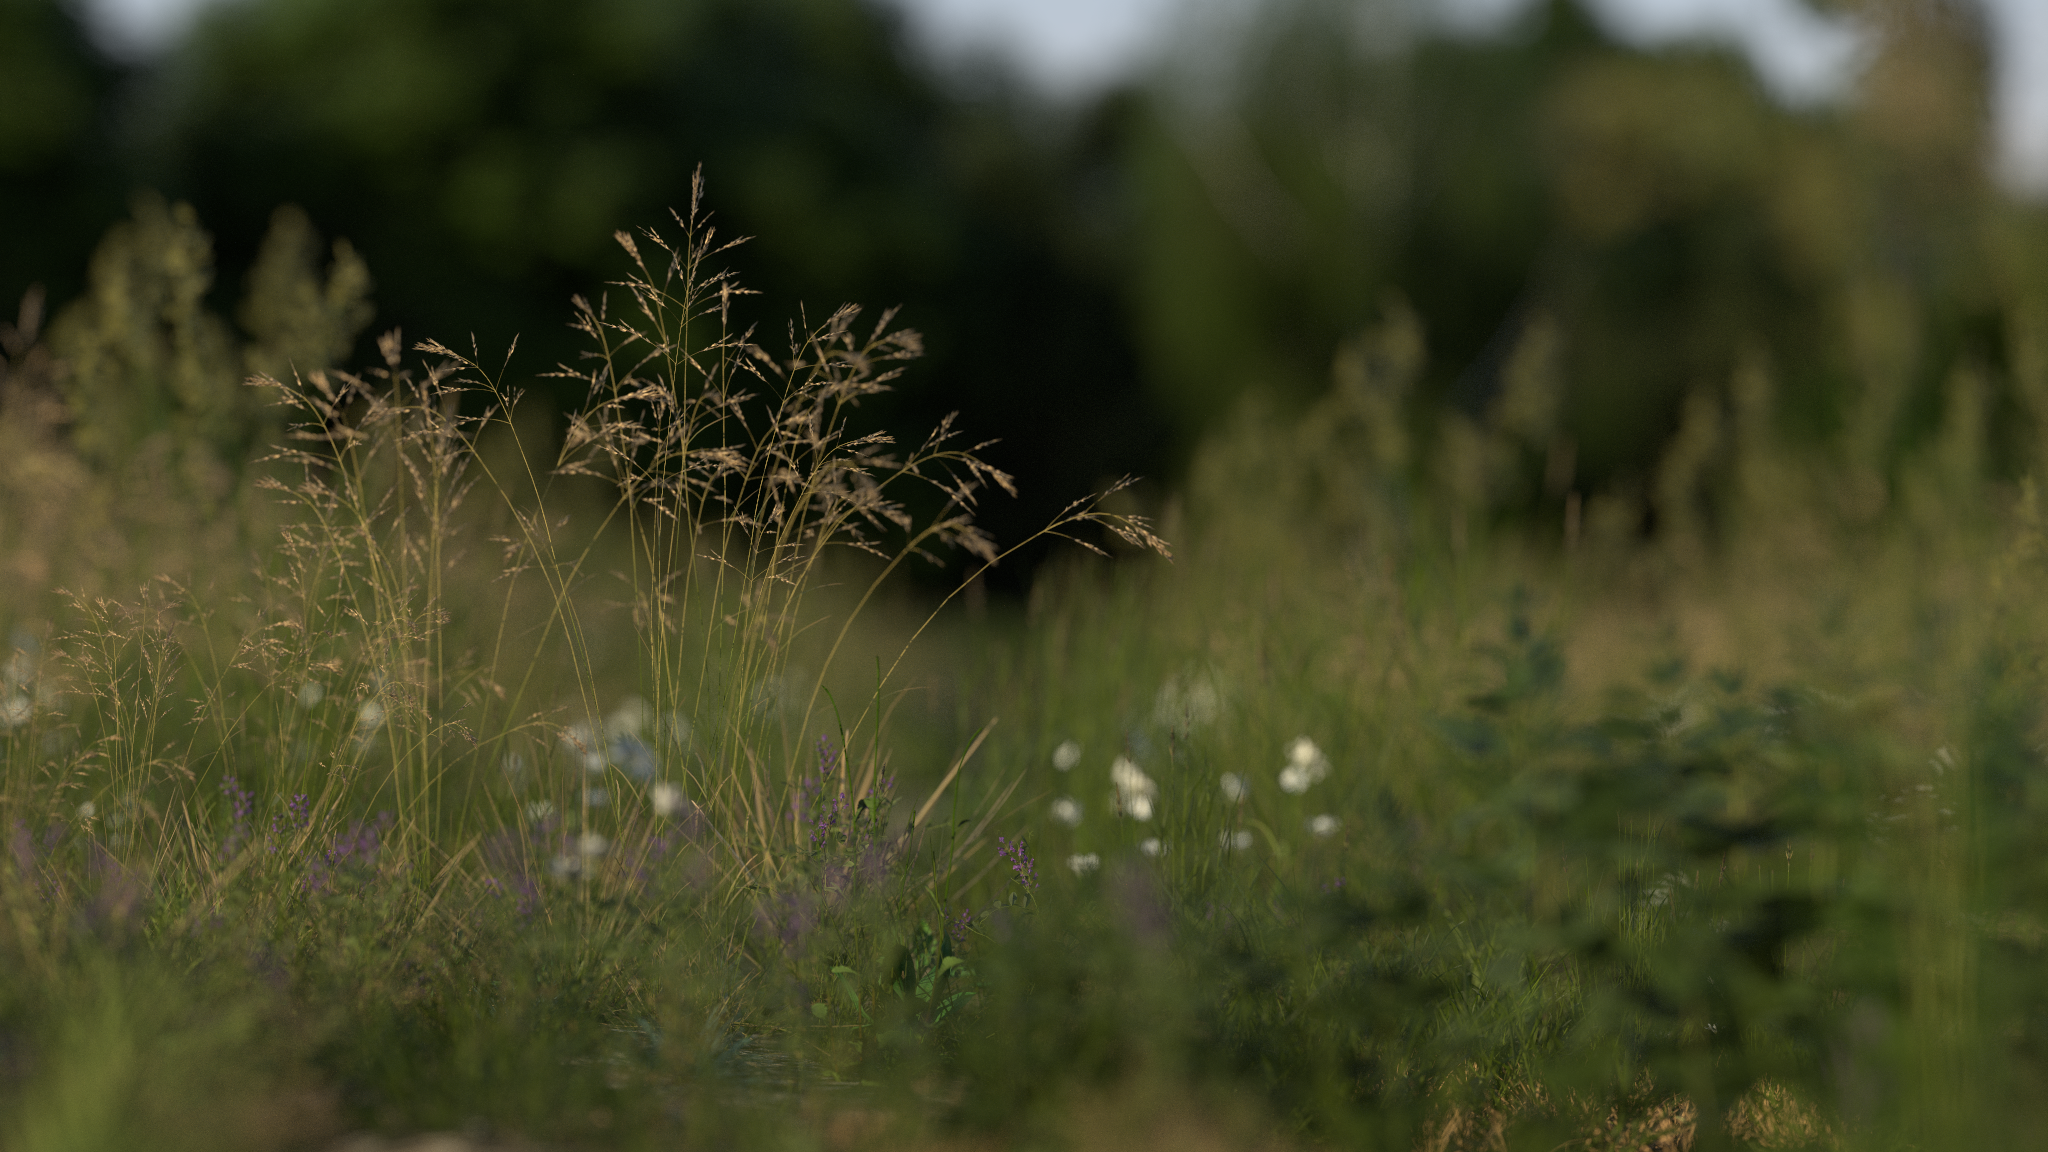
\includegraphics[height=\paperheight]{view-3.png}};
    \draw (current page.center) node [fill=yellow!80!green!40,fill opacity=0.1,text opacity=1,inner sep=1cm]
    {\centering\bfseries\sffamily\parbox[c][][t]{\paperwidth}{\color{white}\centering
    {\Large Physically Based Rendering: From Theory To Implementation}\\[25pt]
    {\fontsize{30pt}{15pt}\textrm{从理论到实现}}\\[15pt]
    {\fontsize{60pt}{15pt}\textrm{基于物理的渲染}}\\[25pt]
    {\fontsize{21pt}{15pt}第三版}\\[20pt]
    {\Large\begin{tabular}{rcl}原著 && Matt Pharr\\ && Wenzel Jakob\\ && Greg Humphreys\\ 翻译 && Kanition\end{tabular}}}};
\end{tikzpicture}
\vfill
\endgroup

%----------------------------------------------------------------------------------------
%	COPYRIGHT PAGE
%----------------------------------------------------------------------------------------

\newpage
~\vfill
\thispagestyle{empty}

\noindent \textbf{\LARGE 从理论到实现}\vspace{8pt}\\
\noindent \textbf{\Huge 基于物理的渲染}\vspace{8pt}\\
\noindent \textbf{\large 第三版}\vspace{8pt}\\
\noindent \textbf{\large 原著 \quad Matt Pharr, Wenzel Jakob \& Greg Humphreys}\vspace{5pt}\\
\noindent \textbf{\large 翻译 \quad Kanition}\vspace{16pt}\\

\noindent {\bfseries 英文原版}

\noindent Copyright \copyright\ 2004–2021 Matt Pharr, Wenzel Jakob, and Greg Humphreys

\noindent 官方网址:\url{http://www.pbr-book.org}

\noindent 许可证:CC BY-NC-SA 4.0\\

\noindent {\bfseries 本中译版}

\noindent Copyright \copyright\ 2021 Kanition

\noindent 更新网址:\url{https://github.com/kanition/pbrtbook}

\noindent 许可证:CC BY-NC-SA 4.0

    {\small(详见:\url{https://creativecommons.org/licenses/by-nc-sa/4.0})}\\

\noindent{\itshape
本中译版(以下简称“本书”)系译者(笔名 Kanition)自学英文经典书籍
《Physically Based Rendering: From Theory To Implementation》第三版时自行翻译而成。
使用本书及其源码须遵循相关许可证协议。

本书在翻译时并不完全遵照原书编排,而是根据我自己的学习情况作出了调整,
包括但不限于调整顺序、增删内容、修改内容。
例如扩展阅读和高阶内容部分往往超出了我的能力范围,这些内容可能会被省略;
再如有一些公式可能存在笔误,我会改写并注明。

此外,翻译并不追求从英语单词到中文字词的“一一映射”。
一些不涉及关键概念的词句可能会依据中文习惯作出修改,
只要表达了作者的核心原意即可。
因此发现英文原版词句和本书内容不完全对应是非常正常和常见的现象。

原书在线版本以网页形式呈现,可以方便地展开、折叠示例代码,但翻译制作成本书时则面临困难。
本书将视具体上下文情况对示例代码做补全、删减或修改。实践时请以原书所附代码为准。

本书由{\scshape \LaTeX} 编写而成,源码已经发布在上述网址,欢迎访问获取最新版。

{\sffamily{欢迎提出宝贵意见和建议。如果你发现本书存在错误,请一定要告诉我们!
讨论区:{\normalfont\url{https://github.com/kanition/pbrtbook/discussions}}}}
}

\newpage
\setcounter{page}{1}
\pagestyle{fancy}
{\Huge\bfseries 前言}\vspace{30pt}\\

渲染是计算机图形学的基础组成部分。
最抽象地说,渲染是把三维场景描述转换为图像的过程。
动画算法、几何建模、材质贴图和计算机图形学其他领域
都须经某些渲染过程来可视化其结果。
从电影到游戏等,渲染无处不在,它为创作、娱乐和可视化开辟了新的领域。

早期的渲染研究重点解决基本问题,例如从给定视点确定哪些物体是可见的。
随着这些问题找到高效解法以及图形学其他领域的持续发展使得场景描述更加丰富逼真,
现代渲染已涵盖了广泛内容,包括物理学、天体物理学、天文学、生物学、心理学、感知研究、理论和应用数学。
渲染的跨学科性是它如此引人的原因之一。

本书以文档化代码的形式提供了构建一个完整的渲染系统所需的一批现代渲染算法。
包括封面在内\sidenote{译者注:本书封面作了更换,但和原书封面是同一组渲染结果。},
本书几乎所有图像都由该软件渲染得到。
且生成这些图像的全部算法均有描述。
该pbrt系统按{\itshape 文学编程}的程序设计方法编写,
即把对系统的描述和实现源码结合在一起。
我们认为,用文学编程法介绍计算机图形学和计算机科学是非常合适的。
算法的一些微妙细节在实现之前往往很难弄清楚,
因此读实际代码更有利于充分理解它们。
我们相信,深入理解哪怕少量的算法也比跑马观花更能打牢进一步研究计算机图形学的基础。

除了阐明实践中如何实现算法外,交代其在完整简单软件系统中的上下文
同样有助于解决中型渲染系统的设计和实现问题。
渲染系统的基本抽象和接口设计对实现的优雅性和可扩展性有实质影响,
但本书不会讨论这类设计取舍。

pbrt和本书内容仅关注{\itshape 逼真渲染},
它可定义为这样的图像生成任务:和相机拍摄的照片难以区分,
或者人类看后被激发的响应与看到实际场景时一致。
我们有许多理由关注逼真感。
逼真图像对电影特效工业至关重要,
因为计算机生成的图像经常必须和真实世界的镜头无缝结合。
娱乐应用中所有图像都是合成的,
逼真感是让观察者忘记所见场景并不实际存在的有效手段。
最后,逼真感为衡量渲染系统输出质量提供了定义合理的指标。\\

\noindent{\LARGE\bfseries 读者}

本书主要面向三类读者。
第一类是学习计算机图形学课程的研究生或高年级本科生。
本书假定读者拥有大学入门级计算机图形学知识,
只会回顾一些关键概念,例如基本向量几何和变换。
对于没有编写过上万行源码程序的学生,
文学编程风格更能降低学习难度。
为了让读者领会为何要这样构建系统,
我们特别注意解释关键接口和抽象背后的设计考量。

第二类读者是计算机图形学研究人员。
本书为研究人员全面介绍了该领域,
pbrt源码提供了可用的构建基础(至少可使用一部分源码)。
对于其他领域的读者,
我们认为对透彻理解渲染也有助于了解相关背景。

最后一类读者是工业界软件开发者。
尽管这些读者可能很熟悉本书许多内容,
但阅读文学风格的算法解释也许能获取新的角度。
pbrt涵盖了大量高级或艰深算法的实现和技术,
例如细分曲面、蒙特卡洛采样算法、双向路径追踪、Metropolis采样和次表面散射;
经验丰富的渲染从业者应该会很感兴趣。
我们希望能激发这些读者去钻研一个完整而典型的渲染系统的兴趣。\\

\noindent{\LARGE\bfseries 概述和目标}

pbrt基于{\itshape 光线追踪}算法。
光线追踪是一项优雅的技术,起源于镜片制造。
19世纪Carl Friedrich Gau{\ss}就用透镜手动追踪光线。
计算机上的光线追踪算法跟随无穷小的光线穿过场景直到与曲面相交。
它给出了从特定位置和方向寻找第一个可见物体的简单方法,
这是许多渲染算法的基础。

pbrt的设计和实现贯彻了三个目标:{\itshape 完整性}、{\itshape 解说性}和基于{\itshape 物理性}。

完整性指系统不应缺少高质量商业渲染系统的关键功能。
这意味着要彻底解决重要的实际问题,
例如抗锯齿、稳定性、数值精度以及高效渲染复杂场景的能力。
在设计系统时一开始就应考虑到这些,
因为它们会对系统所有组件产生微妙影响,
且在实现后期阶段很难再改装到系统中。

第二个目标意味着我们着眼于可读性和清晰度,
精心选用算法、数据结构和渲染技术。
因为比起其他渲染系统,我们的实现要接受更多读者的检验,
所以我们尽力选择已知的最优算法并将其实现。
这个目标也要求系统要小到一个人能完全理解的程度。
我们用可扩展的架构实现了pbrt,
即系统核心采用精心设计的抽象基类,
且这些基类尽量实现足够多特定功能。
这样读者不用理解所有特定细节就能明白系统的基本结构。
这更易于钻研感兴趣的部分并跳过其他内容,
且不影响对系统整体配合的把握。

完整性和解说性目标之间是存在矛盾的。
涵盖所有可能有用的技术不仅让本书过于冗长,
而且对于大多数读者而言也太复杂。
针对万一pbrt缺少某项有用功能的情况,
我们尽量使架构便于增添功能而不用改变系统整体设计。

基于物理的渲染的基础是物理定律及其数学表达式。
pbrt的设计对所计算的量和实现的算法使用正确的物理单位。
这样配置后,pbrt能计算出{\itshape 物理正确}的图像;
它们像在真实世界场景中那样准确反映光照。
这样的好处是它为程序正确性提供了具体标准:
对于预期结果可用闭式解计算的简单场景,
如果pbrt没有算出相同结果,我们就能知道实现一定有bug。
类似地,如果pbrt中基于物理光照的不同算法对同一场景给出了不同结果,
或者pbrt所得结果和另一个基于物理的渲染器不一致,
则它们中必有一个出错了。
最后,我们认为基于物理的渲染方法是有价值的,因为它是严格的。
当不清楚特定计算该如何执行时,物理学会给出确保一致的答案。

效率的优先度低于以上三个目标。
既然渲染系统生成一张图像通常要花费数分钟或小时,
效率显然是很重要的。
然而我们主要关注{\itshape 算法}层面的效率而非底层代码优化。
尽管系统中计算量集中的部分已尽力做了优化,
但有时明显而微小的优化会让位于清晰的代码组织。

在介绍pbrt和讨论其实现时,
我们希望传授多年来渲染研究和开发的经验教训。
编写好一个渲染器比串接一堆快速算法更需要付出;
让系统既灵活又稳定是项困难的任务。
随着增添越来越多的几何体或光源,
或者其他复杂维度上升,
系统的性能将逐渐下降。
严谨处理数值稳定性、
算法不浪费浮点精度也至关重要。

开发出解决所有这些问题的系统大有益处——
编写新的渲染器或向已有渲染器添加新功能并用它创作出以往无法生成的图片是多么地快乐。
我们编写本书最基本的目标就是给广大读者这样的机会。
我们鼓励读者在阅读本书时使用该系统渲染pbrt发行的示例场景。
每章末的习题会要求修改系统以加深对内部工作原理的理解,
或者完成添加新功能等更复杂的工程。

本书官网为\url{www.pbrt.org},
可从该站获取pbrt最新版源码。
我们也会发布勘误、修复bug、新增渲染场景和补充材料。
遇到网站尚未列出的pbrt中的任何bug或行文错误
均发送到邮箱\href{mailto:bugs@pbrt.org}{\url{bugs@pbrt.org}}。
我们非常重视您的反馈\sidenote{译者注:我也欢迎您的反馈!详见扉页更新网址。}!\\

\noindent{\LARGE\bfseries 第一版和第二版的区别}

{\itshape 详见英文原版}\\

\noindent{\LARGE\bfseries 第二版和第三版的区别}

{\itshape 详见英文原版}\\

\noindent{\LARGE\bfseries 致谢}

{\itshape 详见英文原版}\\

\noindent{\LARGE\bfseries 出版}

{\itshape 详见英文原版}\\

\noindent{\LARGE\bfseries 场景和模型}

{\itshape 详见英文原版}\\

\noindent{\LARGE\bfseries 关于封面}

{\itshape 详见英文原版}\\

\noindent{\LARGE\bfseries 扩展阅读}

Donald Knuth的论文《Literate Programming》\citep{10.1093/comjnl/27.2.97}
描述了文学编程背后的主要思想以及他的网络编程环境。
开创性的\TeX 排版系统是用网络写成的并出版了一系列书籍\citep{10.5555/536126,10.5555/536123}。
最近,Knuth在《The Stanford GraphBase》\citep{10.1145/164984}中
以文学格式出版了图表算法集。
这些程序读起来很有趣,各个算法也展示得很好。
网站\url{www.literateprogramming.com}指向了许多关于文学编程的论文、程序以及大量系统;
自Knuth最初提出该思想以来,文学编程已经进行了许多改进。


我们所知的其他出版成书的文学程序只有对lcc编译器的实现——
由Christopher Fraser和David Hanson编写
并出版的《A Retargetable C Compiler: Design and Implementation》\citep{10.5555/555424},
以及Martin Ruckert关于MP3音频格式的书《Understanding MP3》\citep{10.5555/1036653}。


\newpage
{\Huge\bfseries 在线版序言}\vspace{30pt}\\

2004年发行的第一版《基于物理的渲染》只有纸质书。
2010年第二版新增了Kindle版,但不幸的是
所有交叉引用和索引都在转换中丢失了。
终于,2016年发布的第三版转换出了良好的Kindle版和PDF版。
尽管电子版有所改进,但我们觉得它还远称不上完美。

文学编程是《基于物理的渲染》的核心。
它是Donald Knuth提出的一种软件编写方法,
比起在计算机上把源码转换为可执行指令,
它更重视人类阅读源码时的直观性。
文学编程将复杂程序分解为便于理解的片段,
并提供多种方式对其交叉引用,以帮助理解每个片段的内容。

对于纸上的文学编程,每页都有丰富的辅助信息并编有定向页码。
边栏有索引指向当前页所用标识符对应的代码定义所在的页码,
并且每个代码段都有表示其它部分定义所在页码和被引用的页码。

这种格式很有效,但页码绕得烦人。
而且翻书找页也很麻烦。
我们想到,如果把电子设备——台式机、笔记本、平板甚至手机——
作为本书内容的主要交付工具,我们会获得怎样的阅读体验?
没有页码了,取而代之的是超链接,直接把读者引向目标且容易返回原处。

改善的不仅只有导航:
现代显示器比打印纸有好得多的色彩保真度和动态范围,
结合计算机使用还能与书中图示交互。
对于通篇在讲图像与三维世界的书籍而言这是极大的优点。

2018年夏季,我们获取到出版商的授权;
我们非常感谢他们慷慨归还版权。
这样我们就能自由决定是否尝试以这种新形式呈现本书内容。
我们的答案是肯定的。
遭受一个月的黑客攻击后,
我们实现了一个系统,
把本书从以前编写时所用的标记语言转换为HTML。
你现在读的就是它\sidenote{译者注:原作者可能没料到有人又把它翻译回PDF了。}。

本书在线版与第三版《基于物理的渲染》很接近。
我们只作了以下修改:
\begin{itemize}
    \item 更新一些插图所用的渲染图像,
    \item 为图像查看增加交互,
    \item 重画所有插图,
    \item 把比较同一场景的不同渲染结果的多幅图像合并为一幅图像,
    \item 合并读者反馈的勘误。
\end{itemize}

前两点还需要说明一下。关于更新图像:
纸质书的一大挑战是确保诸如蒙特卡洛噪声等图像痕迹在页面上可见。
我们担心印刷会引入多余的模糊,
也担心成书过程中有好心人帮倒忙给图像降噪使其看起来更清晰。
因此我们用最近邻滤波器放大了本应展现差错的图像,
使这些差错能在印刷过程中保留下来。

现在这个担心是多余的了。
很高兴能重新渲染这些图像,
连一个像素大小的差错都能保留了。

第二点修改标志着我们朝交互式内容探究迈出了第一步:
在网页浏览器中,可以细究渲染图像的细节和区别,
这是纸质书做不到的。
在线版大多数渲染图像都能放大、全屏查看以及和其他图像比较。
它们都有此图标
\sidenote{译者注:在线版是一片雪花图案。
    不过PDF没法实现网页端那么强大的交互功能,
    所以阅读本书时就无视它吧。}:*。
将鼠标悬停在该图标上可获取相关操作的详细信息。\\

\noindent{\LARGE\bfseries 路线图}

本书计划大致每年发布一次更新
\sidenote{译者注:本书在翻译时已经发布第四版代码了,但还未在线发布书籍。}。
尽管在线版比纸质版更容易快速更新,
我们还是认为适当的更新速度有利于对下次发布做严谨的检查和编辑。

除了扩展pbrt功能跟进最新研究,
我们还计划为新版增加更多交互元素。
Str{\"o}m、{\AA}str{\"o}m和Akenine-M{\"o}ller
编写的《\citetitle{4b212a02-105c-42a2-ad5c-91c16a06e815}》\footnote{\citeurl{4b212a02-105c-42a2-ad5c-91c16a06e815}}
一书展现了这种媒体的无限可能。

我们会在线保留本书的早前版本,URL均和首发时保持一致;
新版会放在单独的目录中。
因此链接到此处的内容是安全的,不必担心未来断链
\sidenote{译者注:本中译版不作此承诺。}。\\

\noindent{\LARGE\bfseries 报告错误}

{\itshape 详见英文原版}\\

\noindent{\LARGE\bfseries 致谢}

{\itshape 详见英文原版}\\

\noindent{\LARGE\bfseries 许可证}

{\itshape 详见英文原版}

%----------------------------------------------------------------------------------------
%	TABLE OF CONTENTS
%----------------------------------------------------------------------------------------
\renewcommand{\contentsname}{目录}
\renewcommand{\figurename}{图}
\renewcommand{\tablename}{表}

%\usechapterimagefalse % If you don't want to include a chapter image, use this to toggle images off - it can be enabled later with \usechapterimagetrue

\chapterimage{Pictures/measure-one180-cut1260.png} % Table of contents heading image

\pagestyle{empty} % Disable headers and footers for the following pages

\tableofcontents % Print the table of contents itself

\cleardoublepage % Forces the first chapter to start on an odd page so it's on the right side of the book

\pagestyle{fancy} % Enable headers and footers again

%----------------------------------------------------------------------------------------
%	PART
%----------------------------------------------------------------------------------------

\part{绪论}
\chapterimage{Pictures/chap01/nightsnow-cut1368.png}

\chapter{绪论}\label{chap:绪论}

\keyindex{渲染}{rendering}{render渲染}是
由3D\keyindex{场景}{scene}{}描述生成图像的过程。
显然,这是一项十分庞大的任务,
有许多解决方案。\keyindex{基于物理的}{physically based}{physics物理}
的技术采用模拟现实,
即运用物理学规律对光与物质的\keyindex{相互作用}{interaction}{}建模。
尽管基于物理的方法是实现渲染最容易想到的办法,
但它最近十年才在实践中得到广泛运用。
本章末的\refsec{基于物理的渲染简史}
将给出基于物理的渲染的简史
以及它近来在电影\keyindex{离线渲染}{offline rendering}{render渲染}和
游戏\keyindex{交互式渲染}{interactive rendering}{render渲染}方面的应用。

本书将介绍\emph{pbrt}这一基于\keyindex{光线追踪}{ray-tracing}{ray光线}算法的基于物理的渲染系统。
大多数计算机\keyindex{图形学}{graphics}{}书籍都主讲算法和理论,
偶尔附上一小段代码。
相反,本书将理论和一个功能齐全的渲染系统的完整实现结合起来。
系统的完整代码\footnote{\url{https://github.com/mmp/pbrt-v3}}
可在BSD许可证下获取。
在pbrt网站\url{https://pbrt.org}还可获取示例场景、渲染数据等更多信息。

\section{文学编程}\label{sec:文学编程}

在编写\TeX 排版系统时,Donald Knuth新提出一种简单但具有革命性的
编程方法论:\emph{程序应该写得更便于人类使用而不是更便于计算机理解}。
他将其称作\keyindex{文学编程}{literate programming}{}。
本书(包括本章)就是一个长长的文学程序。
这意味着在阅读本书的过程中,
你会读到pbrt渲染系统的\emph{完整}实现,
而不仅仅是高层叙述。

文学程序是由\keyindex{元语言}{metalanguage}{}
写成的,该语言把文档格式语言(例如\TeX 或HTML)
和编程语言(例如C++)结合起来。
两套分离的系统会这样处理程序:\keyindex{编排器}{weaver}{literate programming文学编程}
把文学程序转换成适合排版的文档,\keyindex{整合器}{tangler}{literate programming文学编程}
则生成可供编译的源码\sidenote{译者注:我不太确定编排器和整合器的翻译是否合适。}。
虽然我们的文学编程系统是自研的,
但很大程度上受到了Norman Ramsey的\emph{noweb}系统的影响。

文学编程元语言提供了两个重要功能。
第一个是把行文与源码结合起来。
这个功能让程序的说明和实际源码一样重要,
促使设计和文档做得更细致。
第二个是提供了与输入编译器的顺序完全不同的向读者展示程序代码的机制。
因此可以按逻辑顺序阐述程序。
每一段具有名称的代码块叫作\keyindex{代码片}{fragment}{},
每个代码片可以通过名称引用其他代码片。

例如,考虑一个负责初始化程序全部全局变量的函数
\footnote{本节的代码仅用作示例,不属于pbrt的一部分。}
{\ttfamily InitGlobals()}:
\begin{lstlisting}
void InitGlobals() {
    nMarbles = 25.7;
    shoeSize = 13;
    dielectric = true;
}
\end{lstlisting}

这个函数虽然很简短,但很难在没有任何上下文的情况下搞懂它。
比如为什么变量{\ttfamily nMarbles}采用浮点值?
刚看这段代码时,
就得在整个程序里寻找每个变量是在哪里声明的、怎么用的,
好弄清它的目的和合法值的含义。
尽管这样的系统结构对编译器来说没问题,
但人类阅读者更愿意看到
每个变量的初始化代码是分开呈现的,
而且最好紧挨着实际声明和使用这些变量的代码。

在文学程序中,可以把\refvar{InitGlobals}{()}写成这样:
\begin{lstlisting}
`\initcode{Function Definitions}{=}`
void `\initvar{InitGlobals}{()}` {
    `\refcode{Initialize Global Variables}{\dag}`
}
\end{lstlisting}

这就定义了称作\refcode{Function Definitions}{}的代码片,
包含了函数\refvar{InitGlobals}{()}的定义。
函数\refvar{InitGlobals}{()}自己又引用了另一
代码片\refcode{Initialize Global Variables}{}。
因为初始化的代码片还没有定义,
所以我们只知道这个函数可能会对全局变量赋值
(然而我们可以通过单击右边的加号\sidenote{译者注:本中译版改为直接点击代码片名称。}向前跳转;
这样可以展开代码片最终全部的代码)。

现在有了代码片名称仅仅是有了正确的抽象层级,
因为还没有声明过任何变量。
之后在程序某处引入全局变量{\ttfamily shoeSize}时,
我们可以这样写:
\begin{lstlisting}
    `\initcode{Initialize Global Variables}{=}\initnext{InitializeGlobalVariables}`
    shoeSize = 13;
\end{lstlisting}

这里我们开始定义\refcode{Initialize Global Variables}{}的内容了。
当文学程序整合成待编译的源码时,
文学编程系统会把代码{\ttfamily shoeSize = 13;}
替换到函数\refvar{InitGlobals}{()}的定义内。
等号后的符号{\codecolor $\downarrow$}表示后续还有代码添加到该代码片。
点击它即可跳转到下一处。

后文我们也许又定义了另一个全局变量{\ttfamily dielectric},
可以这样把它的初始化添到代码片之后:
\begin{lstlisting}
    `\refcode{Initialize Global Variables}{+=}\lastcode{InitializeGlobalVariables}`
    dielectric = true;
\end{lstlisting}

代码片名后的符号{\codecolor +=}表示我们之前已经定义过该代码片了。
此外符号{\codecolor $\uparrow$}回链到
之前\refcode{Initialize Global Variables}{}添加代码的地方。

当整合时,这三个代码片转换为代码:
\begin{lstlisting}
void InitGlobals() {
    `\hypertarget{code:Initialize Global Variables}{\color[RGB]{115,48,11}\scriptsize\rmfamily// Initialize Global Variables}`
    shoeSize = 13;
    dielectric = true;
}
\end{lstlisting}

这样,我们可以把复杂函数分解为逻辑不同的部分,使之更容易理解。
例如我们可以这样把一个复杂函数写作一系列代码片:
\begin{lstlisting}
`\refcode{Function Definitions}{+=}`
void `\initvar{complexFunc}{(int x, int y, double *values)}` {
    `\refcode{Check validity of arguments}{}`
    if (x < y) {
        `\refcode{Swap parameter values}{}`
    }
    `\refcode{Do precomputation before loop}{}`
    `\refcode{Loop through and update \textbackslash mono\{values\} array}{}`
}
\end{lstlisting}

同样,编译时\refvar{complexFunc}{()}内每段代码片的内容都内联展开。
在文档中,我们可以依次介绍每个代码片的实现。
这种分解让我们每次只展示一小段代码,使之更易于理解。
这种编程风格的另一优点是,通过把函数分解为逻辑片,
每片有了单一且明确的目的,可以独立编写、验证、阅读。
一般我们尽量让每段代码片少于10行。

在某种意义上,文学编程系统只是个增强了的宏替换包,
完成重排程序源码的任务。
这变化看似微不足道,但事实上文学编程和其他软件构建系统方法迥然不同。



\section{逼真渲染和光线追踪算法}\label{sec:逼真渲染和光线追踪算法}

逼真渲染的目标是创建3D场景的图像且与同一场景的照片难以区分。
在我们介绍渲染流程之前要重点理解的是,
此处的{\itshape 难以区分}一词不是精确说法,
因为它涉及人类观察者,
不同观察者对同一图像的感知可能是不同的。
尽管本书会涉及少量感知问题,
但明确给出观察者的精确特性是非常困难且远未解决的问题。
绝大多数时候,我们都对针对光及其与物质相互作用的物理仿真感到满意,
并以我们对显示技术的理解尽可能向观察者展示最好的图像。

几乎所有逼真渲染系统都基于光线追踪算法。
光线追踪算法其实很简单;
它跟随光线\sidenote{译者注:原文a ray of light。
    此外会按个人理解把ray译作“光线”或“射线”,把light译作“光”或“光线”。}路径
穿过场景与环境中的物体相互作用并反射。
虽然编写光线追踪器的方法有很多,
但所有这些系统都必须模拟至少一项以下对象和现象:
\begin{itemize}
    \item \keyindex{相机}{cameras}{camera相机}: 相机模型决定了从哪里、怎样观察场景,
          包括场景的图像是怎样记录到传感器上的。
          许多渲染系统从相机处开始生成视线并追踪到场景中。
    \item \keyindex{光线-物体交点}{ray–object intersections}{ray光线}: 此外,我们需要确定
          交点处物体的特定属性,例如表面法线或材质。
          多数光线追踪器都有测试光线与多个物体相交的功能,
          典型的例如沿光线返回最近交点。
    \item \keyindex{光源}{light sources}{light光}: 没有光,渲染场景就没有意义。
          光线追踪器必须对整个场景的光分布建模,
          不仅包括灯光自身的位置,还包括它们向整个场景发散能量的方式。
    \item \keyindex{可见性}{visibility}{}:为了知道给定光是否在表面上一点积累能量,
          必须确认从该点到光源是否存在一条不中断的路径。
          幸运的是,在光线追踪器中这个问题很容易回答,
          因为我们可以构造从表面到光源\sidenote{译者注:原文为light,我按个人理解译作“光源”。}的射线,
          寻找最近的光线-物体交点,
          并比较交点距离和光源距离。
    \item \keyindex{表面散射}{surface scattering}{}:每个物体都必须提供外观描述,
          包括光如何与物体表面相互作用等信息,
          以及再辐射\sidenote{译者注:原文reradiated。}(或散射\sidenote{译者注:原文scattered。})光的性质。
          表面散射模型是典型的参数化模型,
          因此可以模拟各种外观。
    \item \keyindex{间接光传输}{indirect light transport}{light光}\sidenote{译者注:这里把transport译作“传输”是为了
              与下一段propagation译作“传播”区分开,但个人理解似乎就是“传播”的意思。}:因为
          光在一个物体上反射或折射后可能遇到另一个物体,
          所以通常有必要追踪从表面发出的额外光线来捕捉这种效应。
    \item \keyindex{光线传播}{ray propagation}{ray光线}:我们需要知道光在空间中沿光线传播时发生了什么。
          如果渲染真空中的场景,则光能量沿光线保持恒定。
          真正的真空虽然在地球上是罕见的,
          但对许多环境而言是合理的近似。
          更多复杂模型可用于追踪穿过雾、烟、大气等的光线。
\end{itemize}

本节我们将简要讨论以上每个仿真任务。
后续章节我们会展示pbrt底层仿真组件的高级接口,
了解贯穿主渲染循环的单个光线处理过程。
我们还会介绍基于Turner Whitted的
原始光线追踪算法的表面散射模型实现。

\subsection{相机}\label{sub:相机}

几乎每个人都用过\keyindex{相机}{camera}{},熟悉它的基本功能:
你表达记下世界的一张图像的愿望(通常是按按钮或点击屏幕),
然后图像就被记录到\keyindex{胶片}{film}{}或电子传感器上。
最简单的拍照设备之一称作\keyindex{针孔相机}{pinhole camera}{camera相机}。
针孔相机由一端打有小孔的遮光盒组成(\reffig{1.1})。
当孔未被遮挡时,光射进孔落到固定在盒子另一端的相纸上。
虽然它很简单,但这种相机至今仍在使用,常用于艺术目的。
要在胶片上获得足够的光以形成图像需要非常长的曝光时间。
\begin{figure}[h]
    \centering%LaTeX with PSTricks extensions
%%Creator: Inkscape 1.0.1 (3bc2e813f5, 2020-09-07)
%%Please note this file requires PSTricks extensions
\psset{xunit=.5pt,yunit=.5pt,runit=.5pt}
\begin{pspicture}(719.89001465,221.22999573)
{
\newrgbcolor{curcolor}{0 0 0}
\pscustom[linewidth=1,linecolor=curcolor]
{
\newpath
\moveto(180.38,220.31999573)
\lineto(54.38,140.19999573)
\lineto(54.38,1.18999573)
\lineto(180.38,81.30999573)
\closepath
}
}
{
\newrgbcolor{curcolor}{0 0 0}
\pscustom[linewidth=1,linecolor=curcolor]
{
\newpath
\moveto(393.38,220.31999573)
\lineto(267.38,140.19999573)
\lineto(267.38,1.18999573)
\lineto(393.38,81.30999573)
\closepath
}
}
{
\newrgbcolor{curcolor}{0 0 0}
\pscustom[linewidth=1,linecolor=curcolor]
{
\newpath
\moveto(180.02000427,220.5699957)
\lineto(393.23999023,220.5699957)
}
}
{
\newrgbcolor{curcolor}{0.72156864 0.70980394 0.70980394}
\pscustom[linestyle=none,fillstyle=solid,fillcolor=curcolor]
{
\newpath
\moveto(153.14,161.25999573)
\lineto(96.9,125.49999573)
\lineto(96.9,63.44999573)
\lineto(153.14,99.20999573)
\closepath
}
}
{
\newrgbcolor{curcolor}{0 0 0}
\pscustom[linewidth=1,linecolor=curcolor]
{
\newpath
\moveto(153.14,161.25999573)
\lineto(96.9,125.49999573)
\lineto(96.9,63.44999573)
\lineto(153.14,99.20999573)
\closepath
}
}
{
\newrgbcolor{curcolor}{0 0 0}
\pscustom[linewidth=1,linecolor=curcolor]
{
\newpath
\moveto(53.95000076,140.56999207)
\lineto(266.80999756,140.56999207)
}
}
{
\newrgbcolor{curcolor}{0 0 0}
\pscustom[linewidth=1,linecolor=curcolor]
{
\newpath
\moveto(180.02000427,82)
\lineto(393.58999634,82)
}
}
{
\newrgbcolor{curcolor}{0 0 0}
\pscustom[linewidth=1,linecolor=curcolor]
{
\newpath
\moveto(54.31000137,0.5)
\lineto(267.16000366,0.5)
}
}
{
\newrgbcolor{curcolor}{0 0 0}
\pscustom[linewidth=1,linecolor=curcolor]
{
\newpath
\moveto(339.7301427,119.158401)
\curveto(341.5742157,118.06695026)(341.46601021,114.47358161)(339.48845898,111.1323875)
\curveto(337.51090776,107.79119338)(334.41286921,105.96741604)(332.56879621,107.05886679)
\curveto(330.72472322,108.15031754)(330.8329287,111.74368618)(332.81047993,115.0848803)
\curveto(334.78803116,118.42607441)(337.88606971,120.24985175)(339.7301427,119.158401)
\closepath
}
}
{
\newrgbcolor{curcolor}{0 0 0}
\pscustom[linewidth=1,linecolor=curcolor]
{
\newpath
\moveto(576.36,162.31999573)
\lineto(520.12,126.55999573)
\lineto(520.12,64.50999573)
\lineto(576.36,100.26999573)
\closepath
}
}
{
\newrgbcolor{curcolor}{0 0 0}
\pscustom[linewidth=1,linecolor=curcolor]
{
\newpath
\moveto(153.71000671,161.95999527)
\lineto(631.82000732,33.97999573)
}
}
{
\newrgbcolor{curcolor}{0 0 0}
\pscustom[linewidth=1,linecolor=curcolor]
{
\newpath
\moveto(97.04000092,125.74999237)
\lineto(617.29998779,98.77999878)
}
}
{
\newrgbcolor{curcolor}{0 0 0}
\pscustom[linewidth=1,linecolor=curcolor]
{
\newpath
\moveto(96.43000031,63.16999817)
\lineto(673.23999023,182.71999741)
}
}
{
\newrgbcolor{curcolor}{0 0 0}
\pscustom[linewidth=1,linecolor=curcolor]
{
\newpath
\moveto(152.83999634,99.34999847)
\lineto(622.55999756,133.60999298)
}
}
{
\newrgbcolor{curcolor}{0 0 0}
\pscustom[linewidth=0.5,linecolor=curcolor]
{
\newpath
\moveto(379.01000977,47.37998962)
\lineto(338.20001221,103.22999573)
}
}
{
\newrgbcolor{curcolor}{0 0 0}
\pscustom[linewidth=0.5,linecolor=curcolor]
{
\newpath
\moveto(47.15000153,86.3999939)
\lineto(91.18000031,90.69999695)
}
}
{
\newrgbcolor{curcolor}{0 0 0}
\pscustom[linestyle=none,fillstyle=solid,fillcolor=curcolor]
{
\newpath
\moveto(369.586782,39.9484801)
\lineto(369.586782,41.0844801)
\lineto(366.242782,41.0844801)
\curveto(366.498782,41.5644801)(366.722782,42.0764801)(366.898782,42.5724801)
\lineto(365.842782,42.8924801)
\curveto(365.314782,41.4204801)(364.386782,39.9804801)(363.378782,39.0524801)
\curveto(363.570782,38.7964801)(363.890782,38.1884801)(363.986782,37.9484801)
\curveto(364.546782,38.5084801)(365.090782,39.1804801)(365.602782,39.9484801)
\closepath
\moveto(367.378782,30.4284801)
\lineto(367.378782,33.9644801)
\lineto(369.506782,33.9644801)
\lineto(369.506782,35.0524801)
\lineto(367.378782,35.0524801)
\lineto(367.378782,37.2124801)
\lineto(369.186782,37.2124801)
\lineto(369.186782,38.2844801)
\lineto(364.594782,38.2844801)
\lineto(364.594782,37.2124801)
\lineto(366.242782,37.2124801)
\lineto(366.242782,35.0524801)
\lineto(363.842782,35.0524801)
\lineto(363.842782,33.9644801)
\lineto(366.242782,33.9644801)
\lineto(366.242782,30.6524801)
\curveto(366.242782,29.9964801)(365.794782,29.6284801)(365.506782,29.4524801)
\curveto(365.714782,29.1964801)(365.970782,28.7004801)(366.066782,28.4124801)
\curveto(366.354782,28.6844801)(366.802782,28.9244801)(369.922782,30.5564801)
\curveto(369.842782,30.7964801)(369.746782,31.2604801)(369.714782,31.5804801)
\closepath
\moveto(378.034782,37.5964801)
\lineto(374.594782,37.5964801)
\lineto(374.594782,42.7964801)
\lineto(373.394782,42.7964801)
\lineto(373.394782,37.5964801)
\lineto(369.666782,37.5964801)
\lineto(369.666782,36.4284801)
\lineto(373.394782,36.4284801)
\lineto(373.394782,28.3324801)
\lineto(374.594782,28.3324801)
\lineto(374.594782,36.4284801)
\lineto(378.034782,36.4284801)
\closepath
}
}
{
\newrgbcolor{curcolor}{0 0 0}
\pscustom[linestyle=none,fillstyle=solid,fillcolor=curcolor]
{
\newpath
\moveto(386.62675148,42.0444801)
\lineto(386.38675148,41.9644801)
\lineto(379.77875148,41.9644801)
\lineto(379.77875148,40.8604801)
\lineto(385.47475148,40.8604801)
\curveto(384.77075148,40.0284801)(383.82675148,39.1324801)(382.97875148,38.5564801)
\lineto(382.97875148,35.4844801)
\curveto(381.61875148,35.1324801)(380.37075148,34.8124801)(379.42675148,34.5724801)
\lineto(379.68275148,33.3884801)
\lineto(382.97875148,34.3004801)
\lineto(382.97875148,29.8204801)
\curveto(382.97875148,29.5804801)(382.89875148,29.5164801)(382.64275148,29.5004801)
\curveto(382.41875148,29.5004801)(381.60275148,29.5004801)(380.70675148,29.5324801)
\curveto(380.89875148,29.1804801)(381.04275148,28.6684801)(381.09075148,28.3324801)
\curveto(382.25875148,28.3164801)(383.04275148,28.3484801)(383.52275148,28.5404801)
\curveto(383.98675148,28.7484801)(384.13075148,29.0844801)(384.13075148,29.8044801)
\lineto(384.13075148,34.6044801)
\lineto(387.37875148,35.5004801)
\lineto(387.21875148,36.6204801)
\curveto(386.19475148,36.3324801)(385.15475148,36.0444801)(384.13075148,35.7884801)
\lineto(384.13075148,38.0764801)
\curveto(385.29875148,38.9724801)(386.59475148,40.2684801)(387.42675148,41.4524801)
\closepath
\moveto(390.37075148,29.5484801)
\curveto(389.76275148,29.5484801)(389.63475148,29.6924801)(389.63475148,30.5084801)
\lineto(389.63475148,42.5564801)
\lineto(388.46675148,42.5564801)
\lineto(388.46675148,30.5404801)
\curveto(388.46675148,28.9244801)(388.83475148,28.4764801)(390.22675148,28.4764801)
\lineto(392.46675148,28.4764801)
\curveto(393.84275148,28.4764801)(394.14675148,29.3724801)(394.27475148,32.0124801)
\curveto(393.95475148,32.0924801)(393.49075148,32.3004801)(393.20275148,32.5404801)
\curveto(393.12275148,30.1404801)(393.02675148,29.5484801)(392.38675148,29.5484801)
\closepath
}
}
{
\newrgbcolor{curcolor}{0 0 0}
\pscustom[linestyle=none,fillstyle=solid,fillcolor=curcolor]
{
\newpath
\moveto(24.961985,91.8927451)
\lineto(20.801985,91.8927451)
\lineto(21.873985,92.3407451)
\curveto(21.665985,92.9167451)(21.153985,93.7167451)(20.641985,94.3087451)
\lineto(19.585985,93.8927451)
\curveto(20.081985,93.2847451)(20.545985,92.4527451)(20.769985,91.8927451)
\lineto(16.721985,91.8927451)
\lineto(16.721985,90.7887451)
\lineto(24.961985,90.7887451)
\closepath
\moveto(21.761985,89.8447451)
\curveto(22.769985,88.8047451)(23.953985,87.3487451)(24.449985,86.3887451)
\lineto(25.345985,87.1087451)
\curveto(24.817985,88.0527451)(23.617985,89.4447451)(22.593985,90.4527451)
\closepath
\moveto(18.641985,90.3727451)
\curveto(18.065985,89.2527451)(17.057985,87.9087451)(16.017985,87.0607451)
\curveto(16.273985,86.8687451)(16.641985,86.5487451)(16.833985,86.3407451)
\curveto(17.889985,87.2847451)(18.977985,88.6287451)(19.681985,89.9087451)
\closepath
\moveto(12.801985,85.9247451)
\curveto(12.817985,86.5807451)(12.833985,87.2367451)(12.833985,87.8127451)
\lineto(12.833985,88.6767451)
\lineto(14.849985,88.6767451)
\lineto(14.849985,85.9247451)
\closepath
\moveto(14.849985,92.4047451)
\lineto(14.849985,89.7487451)
\lineto(12.833985,89.7487451)
\lineto(12.833985,92.4047451)
\closepath
\moveto(15.937985,93.4767451)
\lineto(11.777985,93.4767451)
\lineto(11.777985,87.7967451)
\curveto(11.777985,85.4607451)(11.697985,82.3247451)(10.641985,80.1007451)
\curveto(10.913985,79.9887451)(11.377985,79.7167451)(11.585985,79.5247451)
\curveto(12.289985,81.0447451)(12.593985,82.9967451)(12.737985,84.8367451)
\lineto(14.849985,84.8367451)
\lineto(14.849985,81.0767451)
\curveto(14.849985,80.8847451)(14.785985,80.8367451)(14.609985,80.8207451)
\curveto(14.465985,80.8207451)(13.921985,80.8047451)(13.361985,80.8367451)
\curveto(13.505985,80.5487451)(13.665985,80.0527451)(13.697985,79.7487451)
\curveto(14.545985,79.7487451)(15.089985,79.7807451)(15.441985,79.9727451)
\curveto(15.809985,80.1647451)(15.937985,80.4847451)(15.937985,81.0767451)
\closepath
\moveto(22.449985,87.5407451)
\curveto(22.081985,86.2127451)(21.489985,85.0127451)(20.689985,83.9727451)
\curveto(19.873985,85.0127451)(19.233985,86.2127451)(18.769985,87.5087451)
\lineto(17.745985,87.2207451)
\curveto(18.273985,85.6847451)(19.009985,84.2927451)(19.937985,83.1087451)
\curveto(18.865985,82.0207451)(17.521985,81.1567451)(15.921985,80.4687451)
\curveto(16.161985,80.2767451)(16.513985,79.8447451)(16.673985,79.5887451)
\curveto(18.257985,80.2767451)(19.585985,81.1567451)(20.673985,82.2447451)
\curveto(21.761985,81.1247451)(23.041985,80.2447451)(24.545985,79.6527451)
\curveto(24.721985,79.9887451)(25.073985,80.4527451)(25.345985,80.7087451)
\curveto(23.841985,81.2047451)(22.545985,82.0367451)(21.457985,83.1247451)
\curveto(22.417985,84.2927451)(23.121985,85.6527451)(23.585985,87.2527451)
\closepath
}
}
{
\newrgbcolor{curcolor}{0 0 0}
\pscustom[linestyle=none,fillstyle=solid,fillcolor=curcolor]
{
\newpath
\moveto(30.22595448,88.9167451)
\lineto(40.48195448,88.9167451)
\lineto(40.48195448,90.1167451)
\lineto(36.00195448,90.1167451)
\lineto(36.00195448,94.2127451)
\lineto(34.75395448,94.2127451)
\lineto(34.75395448,90.1167451)
\lineto(30.22595448,90.1167451)
\lineto(30.22595448,93.8127451)
\lineto(29.00995448,93.8127451)
\lineto(29.00995448,88.5167451)
\curveto(29.00995448,85.7327451)(28.78595448,82.7887451)(26.76995448,80.5327451)
\curveto(27.04195448,80.3247451)(27.48995448,79.8927451)(27.68195448,79.6047451)
\curveto(29.15395448,81.2207451)(29.77795448,83.1567451)(30.03395448,85.1567451)
\lineto(36.75395448,85.1567451)
\lineto(36.75395448,79.6367451)
\lineto(38.01795448,79.6367451)
\lineto(38.01795448,86.3727451)
\lineto(30.16195448,86.3727451)
\curveto(30.20995448,87.0927451)(30.22595448,87.8127451)(30.22595448,88.5327451)
\closepath
}
}
{
\newrgbcolor{curcolor}{0 0 0}
\pscustom[linestyle=none,fillstyle=solid,fillcolor=curcolor]
{
\newpath
\moveto(635.912685,116.5621301)
\lineto(640.824685,116.5621301)
\lineto(640.824685,109.1701301)
\lineto(642.008685,109.1701301)
\lineto(642.008685,117.6181301)
\lineto(634.760685,117.6181301)
\lineto(634.760685,109.1701301)
\lineto(635.912685,109.1701301)
\closepath
\moveto(632.488685,116.3541301)
\curveto(632.200685,116.9461301)(631.576685,117.7621301)(630.968685,118.3541301)
\lineto(630.056685,117.8261301)
\curveto(630.632685,117.2021301)(631.240685,116.3221301)(631.528685,115.7461301)
\closepath
\moveto(634.056685,109.4741301)
\curveto(633.752685,109.8261301)(632.648685,111.1061301)(632.056685,111.7621301)
\curveto(632.808685,112.8341301)(633.464685,114.0501301)(633.912685,115.2661301)
\lineto(633.272685,115.6981301)
\lineto(633.048685,115.6501301)
\lineto(628.616685,115.6501301)
\lineto(628.616685,114.5621301)
\lineto(632.472685,114.5621301)
\curveto(631.544685,112.5461301)(629.848685,110.5461301)(628.232685,109.4421301)
\curveto(628.408685,109.2181301)(628.664685,108.6261301)(628.760685,108.2901301)
\curveto(629.384685,108.7541301)(630.008685,109.3301301)(630.616685,109.9861301)
\lineto(630.616685,103.7941301)
\lineto(631.752685,103.7941301)
\lineto(631.752685,110.6421301)
\curveto(632.312685,109.9221301)(632.984685,109.0101301)(633.304685,108.5301301)
\closepath
\moveto(639.944685,104.9301301)
\curveto(639.480685,104.9301301)(639.352685,105.0421301)(639.352685,105.4901301)
\lineto(639.352685,109.4261301)
\lineto(638.552685,109.4261301)
\curveto(638.792685,110.4021301)(638.872685,111.3301301)(638.872685,112.2101301)
\lineto(638.872685,115.3461301)
\lineto(637.720685,115.3461301)
\lineto(637.720685,112.2421301)
\curveto(637.720685,109.7621301)(637.240685,106.7381301)(633.224685,104.6581301)
\curveto(633.464685,104.4661301)(633.848685,104.0181301)(633.976685,103.7621301)
\curveto(636.360685,105.0261301)(637.608685,106.7061301)(638.248685,108.4181301)
\lineto(638.248685,105.3621301)
\curveto(638.248685,104.3221301)(638.680685,104.0181301)(639.768685,104.0181301)
\lineto(641.224685,104.0181301)
\curveto(642.584685,104.0181301)(642.776685,104.6581301)(642.920685,107.1701301)
\curveto(642.616685,107.2501301)(642.232685,107.4101301)(641.944685,107.6341301)
\curveto(641.864685,105.3461301)(641.784685,104.9301301)(641.240685,104.9301301)
\closepath
}
}
{
\newrgbcolor{curcolor}{0 0 0}
\pscustom[linestyle=none,fillstyle=solid,fillcolor=curcolor]
{
\newpath
\moveto(646.44065448,117.5061301)
\lineto(646.44065448,108.4341301)
\lineto(647.65665448,108.4341301)
\lineto(647.65665448,116.3221301)
\lineto(655.35265448,116.3221301)
\lineto(655.35265448,108.4341301)
\lineto(656.60065448,108.4341301)
\lineto(656.60065448,117.5061301)
\closepath
\moveto(650.79265448,114.8341301)
\curveto(650.64865448,109.2181301)(650.42465448,106.1781301)(644.36065448,104.8021301)
\curveto(644.58465448,104.5621301)(644.92065448,104.0821301)(645.03265448,103.7781301)
\curveto(651.43265448,105.3461301)(651.84865448,108.8021301)(652.02465448,114.8341301)
\closepath
\moveto(651.81665448,109.7941301)
\lineto(651.81665448,105.8261301)
\curveto(651.81665448,104.5141301)(652.29665448,104.1781301)(653.83265448,104.1781301)
\lineto(656.68065448,104.1781301)
\curveto(658.12065448,104.1781301)(658.48865448,104.7701301)(658.63265448,107.2501301)
\curveto(658.31265448,107.3301301)(657.81665448,107.5221301)(657.54465448,107.7301301)
\curveto(657.46465448,105.5861301)(657.35265448,105.2821301)(656.58465448,105.2821301)
\lineto(653.92865448,105.2821301)
\curveto(653.14465448,105.2821301)(652.98465448,105.3621301)(652.98465448,105.8421301)
\lineto(652.98465448,109.7941301)
\closepath
}
}
{
\newrgbcolor{curcolor}{0 0 0}
\pscustom[linestyle=none,fillstyle=solid,fillcolor=curcolor]
{
\newpath
\moveto(663.60862396,118.3381301)
\curveto(662.80862396,115.9221301)(661.51262396,113.5381301)(660.10462396,111.9861301)
\curveto(660.31262396,111.7141301)(660.66462396,111.0901301)(660.79262396,110.8181301)
\curveto(661.25662396,111.3621301)(661.72062396,111.9861301)(662.15262396,112.6581301)
\lineto(662.15262396,103.8101301)
\lineto(663.28862396,103.8101301)
\lineto(663.28862396,114.6261301)
\curveto(663.83262396,115.7141301)(664.32862396,116.8661301)(664.71262396,118.0021301)
\closepath
\moveto(674.74462396,114.0341301)
\lineto(674.74462396,115.1861301)
\lineto(669.97662396,115.1861301)
\lineto(669.97662396,118.3381301)
\lineto(668.82462396,118.3381301)
\lineto(668.82462396,115.1861301)
\lineto(664.34462396,115.1861301)
\lineto(664.34462396,114.0341301)
\lineto(668.10462396,114.0341301)
\curveto(667.12862396,111.3301301)(665.46462396,108.6421301)(663.72062396,107.2341301)
\curveto(663.99262396,107.0261301)(664.37662396,106.6101301)(664.58462396,106.3381301)
\curveto(666.26462396,107.8741301)(667.80062396,110.4981301)(668.82462396,113.2661301)
\lineto(668.82462396,107.8261301)
\lineto(666.21662396,107.8261301)
\lineto(666.21662396,106.7381301)
\lineto(668.82462396,106.7381301)
\lineto(668.82462396,103.8741301)
\lineto(669.97662396,103.8741301)
\lineto(669.97662396,106.7381301)
\lineto(672.55262396,106.7381301)
\lineto(672.55262396,107.8261301)
\lineto(669.97662396,107.8261301)
\lineto(669.97662396,113.3781301)
\curveto(670.95262396,110.5941301)(672.48862396,107.9061301)(674.16862396,106.3701301)
\curveto(674.37662396,106.6901301)(674.77662396,107.1061301)(675.06462396,107.3141301)
\curveto(673.33662396,108.7061301)(671.68862396,111.3621301)(670.74462396,114.0341301)
\closepath
}
}
\end{pspicture}

    \caption{针孔相机}\label{fig:1.1}
\end{figure}

虽然大多数相机都比针孔相机复杂得多,
但针孔相机是仿真的便捷起点。
相机最重要的功能是定义会被记录到胶片上的场景部分。
在\reffig{1.1}中,我们可以看见从针孔到胶片边的连线
是如何构造出延伸到场景中的双锥体的。
不在该锥体内的物体不会在胶片上成像。
因为实际的相机成像形状比锥体更复杂,
我们把这个可能在胶片上成像的空间区域称为\keyindex{视见体}{viewing volume}{}。

针孔相机也可以看作是把胶片平面放置在针孔的\emph{前方}但距离不变(\reffig{1.2})。
注意从孔到胶片的连线正好定义了和之前一样的视见体。
当然,这不是真实相机的实际构建方法,
但对于仿真目的而言它是个方便的抽象。
当胶片(或成像)平面在针孔前时,
针孔也常常改称作\keyindex{眼睛}{eye}{}。
\begin{figure}[h]
    \centering%LaTeX with PSTricks extensions
%%Creator: Inkscape 1.0.1 (3bc2e813f5, 2020-09-07)
%%Please note this file requires PSTricks extensions
\psset{xunit=.5pt,yunit=.5pt,runit=.5pt}
\begin{pspicture}(330.91000366,165.99000549)
{
\newrgbcolor{curcolor}{0 0 0}
\pscustom[linewidth=1,linecolor=curcolor]
{
\newpath
\moveto(67.98000336,94.66000366)
\lineto(330.86999512,75.11000824)
}
}
{
\newrgbcolor{curcolor}{0 0 0}
\pscustom[linewidth=1,linecolor=curcolor]
{
\newpath
\moveto(68.19999695,94.96000671)
\lineto(302.67001343,0.46000671)
}
}
{
\newrgbcolor{curcolor}{0.72156864 0.70980394 0.70980394}
\pscustom[linestyle=none,fillstyle=solid,fillcolor=curcolor]
{
\newpath
\moveto(248.69,143.30000549)
\lineto(192.44,107.54000549)
\lineto(192.44,45.49000549)
\lineto(248.69,81.25000549)
\closepath
}
}
{
\newrgbcolor{curcolor}{0 0 0}
\pscustom[linewidth=1,linecolor=curcolor]
{
\newpath
\moveto(248.69,143.30000549)
\lineto(192.44,107.54000549)
\lineto(192.44,45.49000549)
\lineto(248.69,81.25000549)
\closepath
}
}
{
\newrgbcolor{curcolor}{0 0 0}
\pscustom[linewidth=1,linecolor=curcolor]
{
\newpath
\moveto(68.48000336,94.91000366)
\lineto(330.27999878,121.91000366)
}
}
{
\newrgbcolor{curcolor}{0 0 0}
\pscustom[linewidth=1,linecolor=curcolor]
{
\newpath
\moveto(68.19999695,95.15000916)
\lineto(327.17999268,165.5100055)
}
}
{
\newrgbcolor{curcolor}{0.73333335 0.74117649 0.74901962}
\pscustom[linestyle=none,fillstyle=solid,fillcolor=curcolor]
{
\newpath
\moveto(42.85,111.07000549)
\curveto(49.67,99.89000549)(48.24,89.56000549)(38.92,82.39000549)
\curveto(26.86,92.99000549)(14.6,97.78000549)(5.46,100.99000549)
\curveto(5.85,100.99000549)(6.24,101.06000549)(6.65,101.10000549)
\curveto(17.81,102.23000549)(29.33,103.34000549)(42.85,111.07000549)
\closepath
}
}
{
\newrgbcolor{curcolor}{0 0 0}
\pscustom[linestyle=none,fillstyle=solid,fillcolor=curcolor]
{
\newpath
\moveto(38.92,82.39000549)
\curveto(48.24,89.56000549)(49.67,99.89000549)(42.85,111.07000549)
\curveto(29.33,103.34000549)(17.85,102.23000549)(6.65,101.14000549)
\curveto(6.24,101.14000549)(5.85,101.08000549)(5.46,101.03000549)
\curveto(14.6,97.78000549)(26.86,92.99000549)(38.92,82.39000549)
\closepath
\moveto(44.77,112.21000549)
\curveto(52.03,100.21000549)(50.49,88.68000549)(40.61,80.86000549)
\curveto(42.08,79.51000549)(43.55,78.09000549)(45,76.55000549)
\lineto(43.37,74.99000549)
\curveto(28.71,90.54000549)(12.75,96.11000549)(2.19,99.79000549)
\lineto(0,100.58000549)
\curveto(-1.76754134,97.580174)(-6.32632363,99.74115465)(-5.15315982,102.99994303)
\curveto(-3.979996,106.2587314)(0.91011569,105.01811022)(0.36,101.58000549)
\curveto(0.02896037,97.84195685)(-5.409727,97.83838194)(-5.77137565,101.5534999)
\curveto(-6.1330243,105.26861786)(-0.79575471,106.31402991)(0.25,102.71000549)
\curveto(2.33,102.93000549)(4.37,103.15000549)(6.42,103.34000549)
\curveto(19.66,104.62000549)(32.17,105.80000549)(48.16,117.06000549)
\lineto(49.44,115.24000549)
\curveto(47.86,114.15000549)(46.3,113.15000549)(44.77,112.21000549)
\closepath
}
}
{
\newrgbcolor{curcolor}{1 1 1}
\pscustom[linestyle=none,fillstyle=solid,fillcolor=curcolor]
{
\newpath
\moveto(45.7,95.68000549)
\curveto(44.94,90.87000549)(41.84,87.36000549)(38.79,87.85000549)
\curveto(35.74,88.34000549)(33.88,92.64000549)(34.65,97.44000549)
\curveto(35.42,102.24000549)(38.51,105.77000549)(41.57,105.28000549)
\curveto(44.63,104.79000549)(46.48,100.50000549)(45.7,95.68000549)
\closepath
}
}
{
\newrgbcolor{curcolor}{0.12941177 0.12941177 0.12941177}
\pscustom[linestyle=none,fillstyle=solid,fillcolor=curcolor]
{
\newpath
\moveto(44.66,94.85000549)
\curveto(45.10896351,97.9766758)(41.54030622,100.07343854)(39.02747808,98.16011762)
\curveto(36.51464993,96.2467967)(37.5865553,92.24895382)(40.72,91.85000549)
\curveto(42.90474114,91.0470233)(45.29252279,92.37351826)(45.76503229,94.65268173)
\curveto(46.23754179,96.93184519)(44.57390184,99.09826902)(42.25,99.23000549)
\curveto(39.21982147,100.11379445)(36.63602428,96.89026441)(38.15746695,94.12515283)
\curveto(39.67890962,91.36004126)(43.7847623,91.81734597)(44.66,94.85000549)
\closepath
}
}
{
\newrgbcolor{curcolor}{0 0 0}
\pscustom[linestyle=none,fillstyle=solid,fillcolor=curcolor]
{
\newpath
\moveto(249.84836175,59.90126994)
\lineto(245.68836175,59.90126994)
\lineto(246.76036175,60.34926994)
\curveto(246.55236175,60.92526994)(246.04036175,61.72526994)(245.52836175,62.31726994)
\lineto(244.47236175,61.90126994)
\curveto(244.96836175,61.29326994)(245.43236175,60.46126994)(245.65636175,59.90126994)
\lineto(241.60836175,59.90126994)
\lineto(241.60836175,58.79726994)
\lineto(249.84836175,58.79726994)
\closepath
\moveto(246.64836175,57.85326994)
\curveto(247.65636175,56.81326994)(248.84036175,55.35726994)(249.33636175,54.39726994)
\lineto(250.23236175,55.11726994)
\curveto(249.70436175,56.06126994)(248.50436175,57.45326994)(247.48036175,58.46126994)
\closepath
\moveto(243.52836175,58.38126994)
\curveto(242.95236175,57.26126994)(241.94436175,55.91726994)(240.90436175,55.06926994)
\curveto(241.16036175,54.87726994)(241.52836175,54.55726994)(241.72036175,54.34926994)
\curveto(242.77636175,55.29326994)(243.86436175,56.63726994)(244.56836175,57.91726994)
\closepath
\moveto(237.68836175,53.93326994)
\curveto(237.70436175,54.58926994)(237.72036175,55.24526994)(237.72036175,55.82126994)
\lineto(237.72036175,56.68526994)
\lineto(239.73636175,56.68526994)
\lineto(239.73636175,53.93326994)
\closepath
\moveto(239.73636175,60.41326994)
\lineto(239.73636175,57.75726994)
\lineto(237.72036175,57.75726994)
\lineto(237.72036175,60.41326994)
\closepath
\moveto(240.82436175,61.48526994)
\lineto(236.66436175,61.48526994)
\lineto(236.66436175,55.80526994)
\curveto(236.66436175,53.46926994)(236.58436175,50.33326994)(235.52836175,48.10926994)
\curveto(235.80036175,47.99726994)(236.26436175,47.72526994)(236.47236175,47.53326994)
\curveto(237.17636175,49.05326994)(237.48036175,51.00526994)(237.62436175,52.84526994)
\lineto(239.73636175,52.84526994)
\lineto(239.73636175,49.08526994)
\curveto(239.73636175,48.89326994)(239.67236175,48.84526994)(239.49636175,48.82926994)
\curveto(239.35236175,48.82926994)(238.80836175,48.81326994)(238.24836175,48.84526994)
\curveto(238.39236175,48.55726994)(238.55236175,48.06126994)(238.58436175,47.75726994)
\curveto(239.43236175,47.75726994)(239.97636175,47.78926994)(240.32836175,47.98126994)
\curveto(240.69636175,48.17326994)(240.82436175,48.49326994)(240.82436175,49.08526994)
\closepath
\moveto(247.33636175,55.54926994)
\curveto(246.96836175,54.22126994)(246.37636175,53.02126994)(245.57636175,51.98126994)
\curveto(244.76036175,53.02126994)(244.12036175,54.22126994)(243.65636175,55.51726994)
\lineto(242.63236175,55.22926994)
\curveto(243.16036175,53.69326994)(243.89636175,52.30126994)(244.82436175,51.11726994)
\curveto(243.75236175,50.02926994)(242.40836175,49.16526994)(240.80836175,48.47726994)
\curveto(241.04836175,48.28526994)(241.40036175,47.85326994)(241.56036175,47.59726994)
\curveto(243.14436175,48.28526994)(244.47236175,49.16526994)(245.56036175,50.25326994)
\curveto(246.64836175,49.13326994)(247.92836175,48.25326994)(249.43236175,47.66126994)
\curveto(249.60836175,47.99726994)(249.96036175,48.46126994)(250.23236175,48.71726994)
\curveto(248.72836175,49.21326994)(247.43236175,50.04526994)(246.34436175,51.13326994)
\curveto(247.30436175,52.30126994)(248.00836175,53.66126994)(248.47236175,55.26126994)
\closepath
}
}
{
\newrgbcolor{curcolor}{0 0 0}
\pscustom[linestyle=none,fillstyle=solid,fillcolor=curcolor]
{
\newpath
\moveto(255.11233123,56.92526994)
\lineto(265.36833123,56.92526994)
\lineto(265.36833123,58.12526994)
\lineto(260.88833123,58.12526994)
\lineto(260.88833123,62.22126994)
\lineto(259.64033123,62.22126994)
\lineto(259.64033123,58.12526994)
\lineto(255.11233123,58.12526994)
\lineto(255.11233123,61.82126994)
\lineto(253.89633123,61.82126994)
\lineto(253.89633123,56.52526994)
\curveto(253.89633123,53.74126994)(253.67233123,50.79726994)(251.65633123,48.54126994)
\curveto(251.92833123,48.33326994)(252.37633123,47.90126994)(252.56833123,47.61326994)
\curveto(254.04033123,49.22926994)(254.66433123,51.16526994)(254.92033123,53.16526994)
\lineto(261.64033123,53.16526994)
\lineto(261.64033123,47.64526994)
\lineto(262.90433123,47.64526994)
\lineto(262.90433123,54.38126994)
\lineto(255.04833123,54.38126994)
\curveto(255.09633123,55.10126994)(255.11233123,55.82126994)(255.11233123,56.54126994)
\closepath
}
}
\end{pspicture}

    \caption{当仿真针孔相机时,我们把胶片放在孔前的平面,并把孔改称为\emph{眼睛}。}\label{fig:1.2}
\end{figure}
\section{基于物理的渲染简史}\label{sec:基于物理的渲染简史}



\part{主要几何功能}
\chapterimage{Pictures/chap02/dof-dragons-848.png}

\chapter{几何与变换}\label{chap:几何与变换}
\setcounter{sidenote}{1}

几乎所有非平凡\sidenote{译者注:原文nontrivial。}的图形程序都建立在几何类的基础上。
这些类表示数学概念例如点、向量以及射线。
因为这些类在整个系统中无处不在,所以良好的抽象和高效的实现至关重要。
本章介绍了pbrt几何基础的接口和实现。
注意这些并不是表示实际场景几何体的类(三角形、球体等);
那些类是第\refchap{形状}的主题。

本章几何类在pbrt发行版的文件
\href{https://github.com/mmp/pbrt-v3/tree/master/src/core/geometry.h}{\ttfamily core/geometry.h}
和\href{https://github.com/mmp/pbrt-v3/tree/master/src/core/geometry.cpp}{\ttfamily core/geometry.cpp}
中定义,变换矩阵(\refsec{变换})在文件
\href{https://github.com/mmp/pbrt-v3/tree/master/src/core/transform.h}{\ttfamily core/transform.h}和
\href{https://github.com/mmp/pbrt-v3/tree/master/src/core/transform.cpp}{\ttfamily core/transform.cpp}
中实现。

\section{坐标系统}\label{sec:坐标系统}

按计算机图形学中的经典做法,
pbrt用三个坐标值$x,y$和$z$表示\keyindex{点}{point}{}、
\keyindex{向量}{vector}{}和\keyindex{法向量}{normal vector}{vector向量}。
这些值须在\keyindex{坐标系统}{coordinate system}{}下才有意义,
即定义了空间的原点并给出三个线性独立的向量定义$x,y$和$z$坐标轴。
总之,这样的原点和三个向量称为\keyindex{坐标系}{frame}{}。
给定3D中的任意一点或方向,其$(x,y,z)$坐标值取决于它和坐标系的关系。
\reffig{2.1}以2D形式给出例子说明了这点。
\begin{figure}[htbp]
    \centering%LaTeX with PSTricks extensions
%%Creator: Inkscape 1.0.1 (3bc2e813f5, 2020-09-07)
%%Please note this file requires PSTricks extensions
\psset{xunit=.5pt,yunit=.5pt,runit=.5pt}
\begin{pspicture}(327.3999939,474.47000122)
{
\newrgbcolor{curcolor}{0 0 0}
\pscustom[linewidth=1,linecolor=curcolor]
{
\newpath
\moveto(5.5,318.58000122)
\lineto(5.5,38.68000122)
\lineto(286.4,38.68000122)
}
}
{
\newrgbcolor{curcolor}{0 0 0}
\pscustom[linestyle=none,fillstyle=solid,fillcolor=curcolor]
{
\newpath
\moveto(0,313.67000122)
\lineto(5.5,317.93000122)
\lineto(11.01,313.67000122)
\lineto(5.5,326.68000122)
\closepath
}
}
{
\newrgbcolor{curcolor}{0.65098041 0.65098041 0.65098041}
\pscustom[linestyle=none,fillstyle=solid,fillcolor=curcolor]
{
\newpath
\moveto(1.2,315.22000122)
\lineto(5.5,325.37000122)
\lineto(5.5,318.56000122)
\closepath
}
}
{
\newrgbcolor{curcolor}{0.40000001 0.40000001 0.40000001}
\pscustom[linestyle=none,fillstyle=solid,fillcolor=curcolor]
{
\newpath
\moveto(9.8,315.22000122)
\lineto(5.5,325.37000122)
\lineto(5.5,318.56000122)
\closepath
}
}
{
\newrgbcolor{curcolor}{0 0 0}
\pscustom[linestyle=none,fillstyle=solid,fillcolor=curcolor]
{
\newpath
\moveto(281.49,33.18000122)
\lineto(285.75,38.68000122)
\lineto(281.49,44.18000122)
\lineto(294.5,38.68000122)
\closepath
}
}
{
\newrgbcolor{curcolor}{0.65098041 0.65098041 0.65098041}
\pscustom[linestyle=none,fillstyle=solid,fillcolor=curcolor]
{
\newpath
\moveto(283.05,34.38000122)
\lineto(293.19,38.68000122)
\lineto(286.38,38.68000122)
\closepath
}
}
{
\newrgbcolor{curcolor}{0.40000001 0.40000001 0.40000001}
\pscustom[linestyle=none,fillstyle=solid,fillcolor=curcolor]
{
\newpath
\moveto(283.05,42.98000122)
\lineto(293.19,38.68000122)
\lineto(286.38,38.68000122)
\closepath
}
}
{
\newrgbcolor{curcolor}{0 0 0}
\pscustom[linestyle=none,fillstyle=solid,fillcolor=curcolor]
{
\newpath
\moveto(219,243.68000793)
\curveto(219,249.91677562)(211.46003012,253.03903011)(207.05050397,248.62950396)
\curveto(202.64097782,244.21997781)(205.76323232,236.68000793)(212,236.68000793)
\curveto(218.23676768,236.68000793)(221.35902218,244.21997781)(216.94949603,248.62950396)
\curveto(212.53996988,253.03903011)(205,249.91677562)(205,243.68000793)
\curveto(205,237.44324025)(212.53996988,234.32098576)(216.94949603,238.73051191)
\curveto(221.35902218,243.14003806)(218.23676768,250.68000793)(212,250.68000793)
\curveto(205.76323232,250.68000793)(202.64097782,243.14003806)(207.05050397,238.73051191)
\curveto(211.46003012,234.32098576)(219,237.44324025)(219,243.68000793)
\closepath
}
}
{
\newrgbcolor{curcolor}{0 0 0}
\pscustom[linewidth=1,linecolor=curcolor]
{
\newpath
\moveto(219,243.68000793)
\curveto(219,249.91677562)(211.46003012,253.03903011)(207.05050397,248.62950396)
\curveto(202.64097782,244.21997781)(205.76323232,236.68000793)(212,236.68000793)
\curveto(218.23676768,236.68000793)(221.35902218,244.21997781)(216.94949603,248.62950396)
\curveto(212.53996988,253.03903011)(205,249.91677562)(205,243.68000793)
\curveto(205,237.44324025)(212.53996988,234.32098576)(216.94949603,238.73051191)
\curveto(221.35902218,243.14003806)(218.23676768,250.68000793)(212,250.68000793)
\curveto(205.76323232,250.68000793)(202.64097782,243.14003806)(207.05050397,238.73051191)
\curveto(211.46003012,234.32098576)(219,237.44324025)(219,243.68000793)
\closepath
}
}
{
\newrgbcolor{curcolor}{0 0 0}
\pscustom[linewidth=0.5,linecolor=curcolor]
{
\newpath
\moveto(212.5,38.29998779)
\lineto(212.5,243.68000793)
}
}
{
\newrgbcolor{curcolor}{0 0 0}
\pscustom[linewidth=0.5,linecolor=curcolor]
{
\newpath
\moveto(212.5,36.30000122)
\lineto(212.5,26.33000122)
\lineto(5.56,26.33000122)
\lineto(5.56,36.30000122)
}
}
{
\newrgbcolor{curcolor}{0 0 0}
\pscustom[linewidth=1,linecolor=curcolor,linestyle=dashed,dash=4 4]
{
\newpath
\moveto(257.15,467.24000122)
\lineto(197.77,349.88000122)
\lineto(193.09,340.62000122)
\lineto(320.17,276.32000122)
}
}
{
\newrgbcolor{curcolor}{0 0 0}
\pscustom[linestyle=none,fillstyle=solid,fillcolor=curcolor]
{
\newpath
\moveto(250.02,465.34000122)
\lineto(256.85,466.66000122)
\lineto(259.84,460.37000122)
\lineto(260.81,474.47000122)
\closepath
}
}
{
\newrgbcolor{curcolor}{0.65098041 0.65098041 0.65098041}
\pscustom[linestyle=none,fillstyle=solid,fillcolor=curcolor]
{
\newpath
\moveto(251.8,466.19000122)
\lineto(260.21,473.30000122)
\lineto(257.14,467.22000122)
\closepath
}
}
{
\newrgbcolor{curcolor}{0.40000001 0.40000001 0.40000001}
\pscustom[linestyle=none,fillstyle=solid,fillcolor=curcolor]
{
\newpath
\moveto(259.47,462.31000122)
\lineto(260.21,473.30000122)
\lineto(257.14,467.22000122)
\closepath
}
}
{
\newrgbcolor{curcolor}{0 0 0}
\pscustom[linestyle=none,fillstyle=solid,fillcolor=curcolor]
{
\newpath
\moveto(313.31,273.63000122)
\lineto(319.59,276.61000122)
\lineto(318.27,283.45000122)
\lineto(327.4,272.66000122)
\closepath
}
}
{
\newrgbcolor{curcolor}{0.65098041 0.65098041 0.65098041}
\pscustom[linestyle=none,fillstyle=solid,fillcolor=curcolor]
{
\newpath
\moveto(315.24,274.00000122)
\lineto(326.23,273.25000122)
\lineto(320.15,276.33000122)
\closepath
}
}
{
\newrgbcolor{curcolor}{0.40000001 0.40000001 0.40000001}
\pscustom[linestyle=none,fillstyle=solid,fillcolor=curcolor]
{
\newpath
\moveto(319.12,281.67000122)
\lineto(326.23,273.25000122)
\lineto(320.15,276.33000122)
\closepath
}
}
{
\newrgbcolor{curcolor}{0 0 0}
\pscustom[linewidth=1,linecolor=curcolor]
{
\newpath
\moveto(215.15,249.80000122)
\lineto(251.83,322.30000122)
\lineto(197.77,349.88000122)
}
}
{
\newrgbcolor{curcolor}{0 0 0}
\pscustom[linestyle=none,fillstyle=solid,fillcolor=curcolor]
{
\newpath
\moveto(183.85300767,237.52316943)
\curveto(183.78504651,237.21734418)(183.75106592,237.1833636)(183.71708534,237.14938301)
\curveto(183.61514359,237.11540243)(183.37727951,237.11540243)(183.17339602,237.11540243)
\curveto(182.7996096,237.11540243)(182.39184261,237.11540243)(182.39184261,236.50375194)
\curveto(182.39184261,236.26588786)(182.59572611,236.09598495)(182.83359019,236.09598495)
\curveto(183.44524068,236.09598495)(184.15883292,236.16394611)(184.80446399,236.16394611)
\curveto(185.5860174,236.16394611)(186.40155138,236.09598495)(187.1491242,236.09598495)
\curveto(187.28504654,236.09598495)(187.69281353,236.09598495)(187.69281353,236.74161602)
\curveto(187.69281353,237.11540243)(187.3530077,237.11540243)(187.1491242,237.11540243)
\curveto(186.84329896,237.11540243)(186.46951255,237.11540243)(186.19766789,237.14938301)
\lineto(187.1491242,240.92122771)
\curveto(187.45494945,240.61540246)(188.16854169,240.1396743)(189.3238815,240.1396743)
\curveto(193.0957262,240.1396743)(195.44038641,243.57171317)(195.44038641,246.52802387)
\curveto(195.44038641,249.21248991)(193.43553203,250.09598507)(191.63456114,250.09598507)
\curveto(190.10543491,250.09598507)(188.98407568,249.2464705)(188.64426985,248.94064525)
\curveto(187.79475528,250.09598507)(186.3675708,250.09598507)(186.12970672,250.09598507)
\curveto(185.34815332,250.09598507)(184.70252224,249.65423749)(184.26077467,248.87268408)
\curveto(183.71708534,247.98918893)(183.4112601,246.83384912)(183.4112601,246.73190737)
\curveto(183.4112601,246.42608212)(183.75106592,246.42608212)(183.95494942,246.42608212)
\curveto(184.1928135,246.42608212)(184.26077467,246.42608212)(184.36271641,246.52802387)
\curveto(184.43067758,246.56200445)(184.43067758,246.62996562)(184.56659991,247.17365494)
\curveto(184.9743669,248.90666467)(185.48407565,249.31443166)(186.02776497,249.31443166)
\curveto(186.26562905,249.31443166)(186.53747371,249.2464705)(186.53747371,248.53287826)
\curveto(186.53747371,248.19307243)(186.46951255,247.88724718)(186.40155138,247.58142194)
\closepath
\moveto(188.84815335,247.92122777)
\curveto(189.45980384,248.66880059)(190.47922132,249.31443166)(191.53261939,249.31443166)
\curveto(192.8918427,249.31443166)(192.99378445,248.15909185)(192.99378445,247.68336369)
\curveto(192.99378445,246.56200445)(192.24621163,243.87753841)(191.9064058,243.02802384)
\curveto(191.22679414,241.46491703)(190.17339608,240.92122771)(189.28990092,240.92122771)
\curveto(187.99863878,240.92122771)(187.48893003,241.94064519)(187.48893003,242.17850927)
\lineto(187.52291062,242.48433452)
\closepath
\moveto(188.84815335,247.92122777)
}
}
{
\newrgbcolor{curcolor}{0 0 0}
\pscustom[linestyle=none,fillstyle=solid,fillcolor=curcolor]
{
\newpath
\moveto(230.24069439,340.48560115)
\lineto(228.11913079,338.5184158)
\lineto(220.70478482,342.32258442)
\lineto(220.88072762,342.66549792)
\curveto(224.08256631,343.53595448)(226.45170074,344.37315206)(227.98813092,345.17709064)
\curveto(229.5245611,345.98102922)(230.56065307,346.90509204)(231.09640682,347.9492791)
\curveto(231.50535494,348.74632129)(231.59733428,349.52647573)(231.37234484,350.28974243)
\curveto(231.14735539,351.05300913)(230.69503647,351.6090002)(230.01538809,351.95771566)
\curveto(229.39752593,352.27472971)(228.74793084,352.37777302)(228.06660281,352.26684559)
\curveto(227.39462356,352.15892663)(226.76212717,351.8161077)(226.16911367,351.23838879)
\lineto(225.82620017,351.41433159)
\curveto(226.56714171,352.47812308)(227.41273345,353.15259836)(228.36297539,353.43775743)
\curveto(229.31939595,353.71974636)(230.27644941,353.61505494)(231.23413576,353.12368316)
\curveto(232.25360833,352.60060997)(232.93515136,351.8372487)(233.27876485,350.83359935)
\curveto(233.62855696,349.82677986)(233.57520289,348.87850936)(233.11870266,347.98878784)
\curveto(232.79217819,347.35238981)(232.31736679,346.79207515)(231.69426848,346.30784387)
\curveto(230.72348772,345.54149756)(229.43837402,344.86228081)(227.83892739,344.27019362)
\curveto(225.43817238,343.37897352)(223.95749367,342.85863642)(223.39689126,342.70918232)
\lineto(226.67773936,341.02583771)
\curveto(227.34503049,340.68346253)(227.82419699,340.46883141)(228.11523884,340.38194434)
\curveto(228.41245932,340.29188713)(228.70723712,340.26552453)(228.99957225,340.30285653)
\curveto(229.29507752,340.34636715)(229.5944804,340.46592962)(229.89778089,340.66154395)
\closepath
}
}
{
\newrgbcolor{curcolor}{0 0 0}
\pscustom[linestyle=none,fillstyle=solid,fillcolor=curcolor]
{
\newpath
\moveto(224.76749728,138.20995139)
\curveto(223.64944349,139.12661661)(222.92722241,139.86272656)(222.60083404,140.41828124)
\curveto(222.2813901,140.97383592)(222.12166813,141.5502239)(222.12166813,142.14744518)
\curveto(222.12166813,143.06411039)(222.47583424,143.85230359)(223.18416645,144.51202477)
\curveto(223.89249867,145.17869039)(224.8334694,145.51202319)(226.00707866,145.51202319)
\curveto(227.14596575,145.51202319)(228.06263097,145.2029959)(228.75707432,144.58494133)
\curveto(229.45151766,143.96688675)(229.79873934,143.26202675)(229.79873934,142.47036133)
\curveto(229.79873934,141.94258439)(229.61123963,141.40439079)(229.23624023,140.85578055)
\curveto(228.86124082,140.3071703)(228.07999205,139.66133799)(226.89249393,138.91828361)
\curveto(228.11471422,137.97384066)(228.92374072,137.23078627)(229.31957343,136.68912046)
\curveto(229.84735037,135.98078825)(230.11123884,135.23426165)(230.11123884,134.44954067)
\curveto(230.11123884,133.45648668)(229.73276722,132.60579358)(228.97582397,131.89746137)
\curveto(228.21888072,131.19607358)(227.22582673,130.84537969)(225.99666201,130.84537969)
\curveto(224.65638635,130.84537969)(223.61124911,131.26551792)(222.86125029,132.10579437)
\curveto(222.26402902,132.77940442)(221.96541838,133.51551437)(221.96541838,134.31412421)
\curveto(221.96541838,134.93912323)(222.17375138,135.55717781)(222.59041739,136.16828795)
\curveto(223.01402783,136.78634253)(223.73972113,137.46689701)(224.76749728,138.20995139)
\closepath
\moveto(226.40291137,139.32453297)
\curveto(227.23624338,140.07453178)(227.76402033,140.66480863)(227.9862422,141.0953635)
\curveto(228.20846407,141.53286281)(228.31957501,142.02591759)(228.31957501,142.57452783)
\curveto(228.31957501,143.30369335)(228.11471422,143.87313689)(227.70499264,144.28285847)
\curveto(227.29527107,144.69952448)(226.73624417,144.90785748)(226.02791196,144.90785748)
\curveto(225.31957975,144.90785748)(224.74319177,144.70299669)(224.29874802,144.29327512)
\curveto(223.85430428,143.88355354)(223.63208241,143.40438763)(223.63208241,142.85577739)
\curveto(223.63208241,142.49466685)(223.72236005,142.13355631)(223.90291532,141.77244577)
\curveto(224.09041502,141.41133523)(224.35430349,141.06758577)(224.69458073,140.7411974)
\closepath
\moveto(225.25707984,137.81411869)
\curveto(224.68069187,137.32800834)(224.25360921,136.79675918)(223.97583187,136.2203712)
\curveto(223.69805453,135.65092766)(223.55916586,135.03287308)(223.55916586,134.36620747)
\curveto(223.55916586,133.47037555)(223.80222103,132.75162668)(224.28833137,132.20996087)
\curveto(224.78138615,131.67523949)(225.40638516,131.40787881)(226.16332841,131.40787881)
\curveto(226.91332723,131.40787881)(227.51402072,131.61968403)(227.9654089,132.04329447)
\curveto(228.41679708,132.46690491)(228.64249116,132.98079299)(228.64249116,133.5849587)
\curveto(228.64249116,134.08495791)(228.51054693,134.53287387)(228.24665846,134.92870658)
\curveto(227.75360368,135.66481653)(226.75707747,136.62662056)(225.25707984,137.81411869)
\closepath
}
}
{
\newrgbcolor{curcolor}{0 0 0}
\pscustom[linestyle=none,fillstyle=solid,fillcolor=curcolor]
{
\newpath
\moveto(106.21592934,14.52114139)
\curveto(105.09787555,15.43780661)(104.37565447,16.17391656)(104.0492661,16.72947124)
\curveto(103.72982216,17.28502592)(103.57010019,17.8614139)(103.57010019,18.45863518)
\curveto(103.57010019,19.37530039)(103.9242663,20.16349359)(104.63259851,20.82321477)
\curveto(105.34093073,21.48988039)(106.28190146,21.82321319)(107.45551072,21.82321319)
\curveto(108.59439781,21.82321319)(109.51106303,21.5141859)(110.20550638,20.89613133)
\curveto(110.89994972,20.27807675)(111.2471714,19.57321675)(111.2471714,18.78155133)
\curveto(111.2471714,18.25377439)(111.05967169,17.71558079)(110.68467229,17.16697055)
\curveto(110.30967288,16.6183603)(109.52842411,15.97252799)(108.34092599,15.22947361)
\curveto(109.56314628,14.28503066)(110.37217278,13.54197627)(110.76800549,13.00031046)
\curveto(111.29578243,12.29197825)(111.5596709,11.54545165)(111.5596709,10.76073067)
\curveto(111.5596709,9.76767668)(111.18119928,8.91698358)(110.42425603,8.20865137)
\curveto(109.66731278,7.50726358)(108.67425879,7.15656969)(107.44509407,7.15656969)
\curveto(106.10481841,7.15656969)(105.05968117,7.57670792)(104.30968235,8.41698437)
\curveto(103.71246108,9.09059442)(103.41385044,9.82670437)(103.41385044,10.62531421)
\curveto(103.41385044,11.25031323)(103.62218344,11.86836781)(104.03884945,12.47947795)
\curveto(104.46245989,13.09753253)(105.18815319,13.77808701)(106.21592934,14.52114139)
\closepath
\moveto(107.85134343,15.63572297)
\curveto(108.68467544,16.38572178)(109.21245239,16.97599863)(109.43467426,17.4065535)
\curveto(109.65689613,17.84405281)(109.76800707,18.33710759)(109.76800707,18.88571783)
\curveto(109.76800707,19.61488335)(109.56314628,20.18432689)(109.1534247,20.59404847)
\curveto(108.74370313,21.01071448)(108.18467623,21.21904748)(107.47634402,21.21904748)
\curveto(106.76801181,21.21904748)(106.19162383,21.01418669)(105.74718008,20.60446512)
\curveto(105.30273634,20.19474354)(105.08051447,19.71557763)(105.08051447,19.16696739)
\curveto(105.08051447,18.80585685)(105.17079211,18.44474631)(105.35134738,18.08363577)
\curveto(105.53884708,17.72252523)(105.80273555,17.37877577)(106.14301279,17.0523874)
\closepath
\moveto(106.7055119,14.12530869)
\curveto(106.12912393,13.63919834)(105.70204127,13.10794918)(105.42426393,12.5315612)
\curveto(105.14648659,11.96211766)(105.00759792,11.34406308)(105.00759792,10.67739747)
\curveto(105.00759792,9.78156555)(105.25065309,9.06281668)(105.73676343,8.52115087)
\curveto(106.22981821,7.98642949)(106.85481722,7.71906881)(107.61176047,7.71906881)
\curveto(108.36175929,7.71906881)(108.96245278,7.93087403)(109.41384096,8.35448447)
\curveto(109.86522914,8.77809491)(110.09092322,9.29198299)(110.09092322,9.8961487)
\curveto(110.09092322,10.39614791)(109.95897899,10.84406387)(109.69509052,11.23989658)
\curveto(109.20203574,11.97600653)(108.20550953,12.93781056)(106.7055119,14.12530869)
\closepath
}
}
{
\newrgbcolor{curcolor}{0 0 0}
\pscustom[linestyle=none,fillstyle=solid,fillcolor=curcolor]
{
\newpath
\moveto(235.10634431,277.72855707)
\lineto(239.29893945,275.57741132)
\lineto(238.6706551,274.3528816)
\lineto(234.47805996,276.50402735)
\closepath
}
}
{
\newrgbcolor{curcolor}{0 0 0}
\pscustom[linestyle=none,fillstyle=solid,fillcolor=curcolor]
{
\newpath
\moveto(247.54661029,270.98712763)
\lineto(246.95577335,269.83558313)
\lineto(245.47985011,270.59285301)
\lineto(243.99027529,267.68966334)
\lineto(242.65221302,268.37619922)
\lineto(244.14178783,271.27938889)
\lineto(239.486953,273.66770158)
\lineto(240.01953841,274.70571353)
\lineto(248.85681351,279.37085812)
\lineto(249.74885503,278.91316754)
\lineto(246.07068705,271.74439751)
\closepath
\moveto(244.73262477,272.43093339)
\lineto(247.53285899,277.88860559)
\lineto(240.87251783,274.41148538)
\closepath
}
}
\end{pspicture}

    \caption{2D中,点$\bm p$的坐标$(x,y)$由该点与特定2D坐标系统的关系定义。
        这里展示了两个坐标系统;
        该点关于实线坐标系统的坐标为$(8,8)$,但关于虚线坐标系统的坐标为$(2,-4)$。
        两种情况下,2D点$\bm p$都处于空间中的同一绝对位置。}
    \label{fig:2.1}
\end{figure}

在一般的$n$维情形下,坐标系原点$\bm p_\mathrm{o}$及其
$n$个线性独立的\keyindex{基向量}{basis vector}{vector向量}定义了一个$n$维\keyindex{仿射空间}{affine space}{}。
该空间内所有向量$\bm v$都能表示为基向量的线性组合。
给定向量$\bm v$和基向量$\bm v_i$,存在唯一一组标量值$s_i$使得
\begin{align*}
    \bm v=s_1\bm v_1+\cdots+s_n\bm v_n\, .
\end{align*}
标量$s_i$是$\bm v$相对于基$\{\bm v_1,\bm v_2,\ldots \bm v_n\}$的\keyindex{表示}{representation}{},
即我们用向量保存的坐标值。
同样,对于所有点$\bm p$,存在唯一的标量$s_i$使得该点
可以用原点$\bm p_\mathrm{o}$和基向量表示:
\begin{align*}
    \bm p=\bm p_\mathrm{o}+s_1\bm v_1+\cdots+s_n\bm v_n\, .
\end{align*}

因此,尽管3D中的点和向量都用$x,y$和$z$表示,
它们却是不同的数学对象,不能随便互换。

以坐标系统形式定义点和向量造成了一个悖论:
我们需要一个点和一组向量定义坐标系,
但我们只能在特定坐标系下才能有意义地谈论点和向量。
因此,在三维中我们需要一个原点为$(0,0,0)$、
基向量为$(1,0,0)$、$(0,1,0)$以及$(0,0,1)$
的\keyindex{标准坐标系}{standard frame}{frame坐标系}。
其他所有坐标系都参照这个规范坐标系统定义,
该坐标系称为\keyindex{世界空间}{world space}{}。

\subsection{坐标系统惯用手}\label{sub:坐标系统惯用手}
如\reffig{2.2}所示,三个坐标轴有两种排布方式。
给定垂直的$x$和$y$坐标轴,$z$轴可以指向两个方向中的一个。
这两种选择分别称为\keyindex{左手}{left-handed}{}和\keyindex{右手}{right-handed}{}。
任选一种都行但暗含了整个系统中的一些几何操作要如何实现。
pbrt使用左手坐标系统。
\begin{figure}
    \centering%LaTeX with PSTricks extensions
%%Creator: Inkscape 1.0.1 (3bc2e813f5, 2020-09-07)
%%Please note this file requires PSTricks extensions
\psset{xunit=.5pt,yunit=.5pt,runit=.5pt}
\begin{pspicture}(492.61999512,311.95001221)
{
\newrgbcolor{curcolor}{0 0 0}
\pscustom[linewidth=1,linecolor=curcolor]
{
\newpath
\moveto(317.31,282.98001221)
\lineto(317.31,128.95001221)
\lineto(471.91,128.95001221)
}
}
{
\newrgbcolor{curcolor}{0 0 0}
\pscustom[linestyle=none,fillstyle=solid,fillcolor=curcolor]
{
\newpath
\moveto(311.81,278.07001221)
\lineto(317.31,282.33001221)
\lineto(322.81,278.07001221)
\lineto(317.31,291.09001221)
\closepath
}
}
{
\newrgbcolor{curcolor}{0.65098041 0.65098041 0.65098041}
\pscustom[linestyle=none,fillstyle=solid,fillcolor=curcolor]
{
\newpath
\moveto(313.01,279.63001221)
\lineto(317.31,289.77001221)
\lineto(317.31,282.96001221)
\closepath
}
}
{
\newrgbcolor{curcolor}{0.40000001 0.40000001 0.40000001}
\pscustom[linestyle=none,fillstyle=solid,fillcolor=curcolor]
{
\newpath
\moveto(321.61,279.63001221)
\lineto(317.31,289.77001221)
\lineto(317.31,282.96001221)
\closepath
}
}
{
\newrgbcolor{curcolor}{0 0 0}
\pscustom[linestyle=none,fillstyle=solid,fillcolor=curcolor]
{
\newpath
\moveto(467,123.44001221)
\lineto(471.26,128.95001221)
\lineto(467,134.45001221)
\lineto(480.01,128.95001221)
\closepath
}
}
{
\newrgbcolor{curcolor}{0.65098041 0.65098041 0.65098041}
\pscustom[linestyle=none,fillstyle=solid,fillcolor=curcolor]
{
\newpath
\moveto(468.56,124.65001221)
\lineto(478.7,128.95001221)
\lineto(471.89,128.95001221)
\closepath
}
}
{
\newrgbcolor{curcolor}{0.40000001 0.40000001 0.40000001}
\pscustom[linestyle=none,fillstyle=solid,fillcolor=curcolor]
{
\newpath
\moveto(468.56,133.24001221)
\lineto(478.7,128.95001221)
\lineto(471.89,128.95001221)
\closepath
}
}
{
\newrgbcolor{curcolor}{0 0 0}
\pscustom[linewidth=1,linecolor=curcolor]
{
\newpath
\moveto(5.5,277.76001221)
\lineto(5.5,123.73001221)
\lineto(160.1,123.73001221)
}
}
{
\newrgbcolor{curcolor}{0 0 0}
\pscustom[linestyle=none,fillstyle=solid,fillcolor=curcolor]
{
\newpath
\moveto(0,272.86001221)
\lineto(5.5,277.11001221)
\lineto(11.01,272.86001221)
\lineto(5.5,285.87001221)
\closepath
}
}
{
\newrgbcolor{curcolor}{0.65098041 0.65098041 0.65098041}
\pscustom[linestyle=none,fillstyle=solid,fillcolor=curcolor]
{
\newpath
\moveto(1.2,274.41001221)
\lineto(5.5,284.56001221)
\lineto(5.5,277.75001221)
\closepath
}
}
{
\newrgbcolor{curcolor}{0.40000001 0.40000001 0.40000001}
\pscustom[linestyle=none,fillstyle=solid,fillcolor=curcolor]
{
\newpath
\moveto(9.8,274.41001221)
\lineto(5.5,284.56001221)
\lineto(5.5,277.75001221)
\closepath
}
}
{
\newrgbcolor{curcolor}{0 0 0}
\pscustom[linestyle=none,fillstyle=solid,fillcolor=curcolor]
{
\newpath
\moveto(155.19,118.23001221)
\lineto(159.45,123.73001221)
\lineto(155.19,129.23001221)
\lineto(168.21,123.73001221)
\closepath
}
}
{
\newrgbcolor{curcolor}{0.65098041 0.65098041 0.65098041}
\pscustom[linestyle=none,fillstyle=solid,fillcolor=curcolor]
{
\newpath
\moveto(156.75,119.43001221)
\lineto(166.89,123.73001221)
\lineto(160.08,123.73001221)
\closepath
}
}
{
\newrgbcolor{curcolor}{0.40000001 0.40000001 0.40000001}
\pscustom[linestyle=none,fillstyle=solid,fillcolor=curcolor]
{
\newpath
\moveto(156.75,128.03001221)
\lineto(166.89,123.73001221)
\lineto(160.08,123.73001221)
\closepath
}
}
{
\newrgbcolor{curcolor}{0 0 0}
\pscustom[linewidth=1,linecolor=curcolor]
{
\newpath
\moveto(114.43000031,232.70001221)
\lineto(5.51999998,123.78001404)
}
}
{
\newrgbcolor{curcolor}{0 0 0}
\pscustom[linestyle=none,fillstyle=solid,fillcolor=curcolor]
{
\newpath
\moveto(107.07,233.12001221)
\lineto(113.97,232.23001221)
\lineto(114.86,225.33001221)
\lineto(120.17,238.42001221)
\closepath
}
}
{
\newrgbcolor{curcolor}{0.65098041 0.65098041 0.65098041}
\pscustom[linestyle=none,fillstyle=solid,fillcolor=curcolor]
{
\newpath
\moveto(109.02,233.37001221)
\lineto(119.24,237.50001221)
\lineto(114.42,232.68001221)
\closepath
}
}
{
\newrgbcolor{curcolor}{0.40000001 0.40000001 0.40000001}
\pscustom[linestyle=none,fillstyle=solid,fillcolor=curcolor]
{
\newpath
\moveto(115.1,227.29001221)
\lineto(119.24,237.50001221)
\lineto(114.42,232.68001221)
\closepath
}
}
{
\newrgbcolor{curcolor}{0 0 0}
\pscustom[linewidth=1,linecolor=curcolor]
{
\newpath
\moveto(317.42999268,129.31001282)
\lineto(208.50999451,20.39001465)
}
}
{
\newrgbcolor{curcolor}{0 0 0}
\pscustom[linestyle=none,fillstyle=solid,fillcolor=curcolor]
{
\newpath
\moveto(208.09,27.75001221)
\lineto(208.97,20.85001221)
\lineto(215.88,19.97001221)
\lineto(202.78,14.66001221)
\closepath
}
}
{
\newrgbcolor{curcolor}{0.65098041 0.65098041 0.65098041}
\pscustom[linestyle=none,fillstyle=solid,fillcolor=curcolor]
{
\newpath
\moveto(207.84,25.80001221)
\lineto(203.71,15.59001221)
\lineto(208.53,20.40001221)
\closepath
}
}
{
\newrgbcolor{curcolor}{0.40000001 0.40000001 0.40000001}
\pscustom[linestyle=none,fillstyle=solid,fillcolor=curcolor]
{
\newpath
\moveto(213.92,19.72001221)
\lineto(203.71,15.59001221)
\lineto(208.53,20.40001221)
\closepath
}
}
{
\newrgbcolor{curcolor}{0 0 0}
\pscustom[linestyle=none,fillstyle=solid,fillcolor=curcolor]
{
\newpath
\moveto(487.1955217,130.8487217)
\curveto(487.3321743,131.3953321)(487.84462155,133.41095795)(489.34780015,133.41095795)
\curveto(489.4502896,133.41095795)(489.9969,133.41095795)(490.44102095,133.13765275)
\curveto(489.82608425,133.00100015)(489.41612645,132.4885529)(489.41612645,131.9419425)
\curveto(489.41612645,131.600311)(489.6552685,131.1903532)(490.23604205,131.1903532)
\curveto(490.71432615,131.1903532)(491.39758915,131.56614785)(491.39758915,132.45438975)
\curveto(491.39758915,133.5817737)(490.1335526,133.88924205)(489.3819633,133.88924205)
\curveto(488.11792675,133.88924205)(487.36633745,132.72769495)(487.09303225,132.24941085)
\curveto(486.54642185,133.68426315)(485.38487475,133.88924205)(484.7357749,133.88924205)
\curveto(482.481007,133.88924205)(481.21697045,131.08786375)(481.21697045,130.54125335)
\curveto(481.21697045,130.3021113)(481.4561125,130.3021113)(481.49027565,130.3021113)
\curveto(481.6610914,130.3021113)(481.7294177,130.3704376)(481.76358085,130.54125335)
\curveto(482.51517015,132.86434755)(483.95002245,133.41095795)(484.70161175,133.41095795)
\curveto(485.11156955,133.41095795)(485.86315885,133.20597905)(485.86315885,131.9419425)
\curveto(485.86315885,131.2586795)(485.4873642,129.8238272)(484.70161175,126.7491437)
\curveto(484.35998025,125.41678085)(483.5742278,124.4943758)(482.6176596,124.4943758)
\curveto(482.481007,124.4943758)(482.0027229,124.4943758)(481.5244388,124.767681)
\curveto(482.0710492,124.9043336)(482.5493333,125.34845455)(482.5493333,125.96339125)
\curveto(482.5493333,126.5441648)(482.0710492,126.71498055)(481.76358085,126.71498055)
\curveto(481.08031785,126.71498055)(480.5678706,126.16837015)(480.5678706,125.450944)
\curveto(480.5678706,124.46021265)(481.62692825,124.0160917)(482.58349645,124.0160917)
\curveto(484.0525119,124.0160917)(484.83826435,125.55343345)(484.8724275,125.6559229)
\curveto(485.1457327,124.87017045)(485.93148515,124.0160917)(487.22968485,124.0160917)
\curveto(489.48445275,124.0160917)(490.71432615,126.81747)(490.71432615,127.3640804)
\curveto(490.71432615,127.60322245)(490.5435104,127.60322245)(490.4751841,127.60322245)
\curveto(490.2702052,127.60322245)(490.23604205,127.500733)(490.16771575,127.3640804)
\curveto(489.4502896,125.00682305)(487.98127415,124.4943758)(487.29801115,124.4943758)
\curveto(486.4439324,124.4943758)(486.1023009,125.1776388)(486.1023009,125.9292281)
\curveto(486.1023009,126.4075122)(486.20479035,126.8857963)(486.4439324,127.8423645)
\closepath
\moveto(487.1955217,130.8487217)
}
}
{
\newrgbcolor{curcolor}{0 0 0}
\pscustom[linestyle=none,fillstyle=solid,fillcolor=curcolor]
{
\newpath
\moveto(321.81166725,305.2585204)
\curveto(321.9141567,305.56598875)(321.9141567,305.6001519)(321.9141567,305.77096765)
\curveto(321.9141567,306.1467623)(321.60668835,306.3517412)(321.26505685,306.3517412)
\curveto(321.06007795,306.3517412)(320.71844645,306.2150886)(320.51346755,305.90762025)
\curveto(320.4793044,305.77096765)(320.2743255,305.1218678)(320.2059992,304.71191)
\curveto(320.03518345,304.1652996)(319.89853085,303.5503629)(319.76187825,302.96958935)
\lineto(318.7711469,299.0408271)
\curveto(318.7028206,298.73335875)(317.7462524,297.196017)(316.3114001,297.196017)
\curveto(315.2181793,297.196017)(314.97903725,298.1525852)(314.97903725,298.9725008)
\curveto(314.97903725,299.96323215)(315.3548319,301.32975815)(316.07225805,303.24289455)
\curveto(316.41388955,304.13113645)(316.516379,304.3702785)(316.516379,304.81439945)
\curveto(316.516379,305.77096765)(315.833116,306.59088325)(314.7398952,306.59088325)
\curveto(312.65594305,306.59088325)(311.8701906,303.4137103)(311.8701906,303.24289455)
\curveto(311.8701906,303.0037525)(312.0751695,303.0037525)(312.10933265,303.0037525)
\curveto(312.3484747,303.0037525)(312.3484747,303.0720788)(312.45096415,303.4137103)
\curveto(313.06590085,305.4634993)(313.9199796,306.11259915)(314.6715689,306.11259915)
\curveto(314.84238465,306.11259915)(315.2181793,306.11259915)(315.2181793,305.42933615)
\curveto(315.2181793,304.88272575)(314.97903725,304.3019522)(314.84238465,303.8919944)
\curveto(313.95414275,301.5689002)(313.5783481,300.3390268)(313.5783481,299.3141323)
\curveto(313.5783481,297.36683275)(314.9448741,296.7177329)(316.2430738,296.7177329)
\curveto(317.09715255,296.7177329)(317.8145787,297.09352755)(318.4295154,297.70846425)
\curveto(318.1562102,296.5810803)(317.882905,295.4878595)(317.02882625,294.3263124)
\curveto(316.4480527,293.60888625)(315.6281371,292.9597864)(314.63740575,292.9597864)
\curveto(314.3299374,292.9597864)(313.33920605,293.0281127)(312.9634114,293.88219145)
\curveto(313.3050429,293.88219145)(313.61251125,293.88219145)(313.88581645,294.15549665)
\curveto(314.1249585,294.3263124)(314.3299374,294.63378075)(314.3299374,295.04373855)
\curveto(314.3299374,295.72700155)(313.74916385,295.79532785)(313.54418495,295.79532785)
\curveto(313.0317377,295.79532785)(312.31431155,295.45369635)(312.31431155,294.3946387)
\curveto(312.31431155,293.3014179)(313.27087975,292.4815023)(314.63740575,292.4815023)
\curveto(316.8580105,292.4815023)(319.1127784,294.462965)(319.7277151,296.9227118)
\closepath
\moveto(321.81166725,305.2585204)
}
}
{
\newrgbcolor{curcolor}{0 0 0}
\pscustom[linestyle=none,fillstyle=solid,fillcolor=curcolor]
{
\newpath
\moveto(127.0204015,239.3646719)
\curveto(128.1819486,240.62870845)(128.83104845,241.17531885)(129.6168009,241.85858185)
\curveto(129.6168009,241.85858185)(130.94916375,243.02012895)(131.7349162,243.8058814)
\curveto(133.81886835,245.82150725)(134.29715245,246.8805649)(134.29715245,246.98305435)
\curveto(134.29715245,247.18803325)(134.09217355,247.18803325)(134.0580104,247.18803325)
\curveto(133.88719465,247.18803325)(133.8530315,247.1538701)(133.7163789,246.9488912)
\curveto(133.06727905,245.88983355)(132.6231581,245.54820205)(132.11071085,245.54820205)
\curveto(131.56410045,245.54820205)(131.3249584,245.88983355)(130.9833269,246.2656282)
\curveto(130.5733691,246.7439123)(130.19757445,247.18803325)(129.4801483,247.18803325)
\curveto(127.8403171,247.18803325)(126.84958575,245.1724074)(126.84958575,244.6941233)
\curveto(126.84958575,244.59163385)(126.91791205,244.45498125)(127.0887278,244.45498125)
\curveto(127.2937067,244.45498125)(127.32786985,244.5574707)(127.39619615,244.6941233)
\curveto(127.80615395,245.7190178)(129.0701905,245.7190178)(129.24100625,245.7190178)
\curveto(129.6851272,245.7190178)(130.095085,245.5823652)(130.60753225,245.41154945)
\curveto(131.49577415,245.06991795)(131.7349162,245.06991795)(132.2815266,245.06991795)
\curveto(131.49577415,244.1475129)(129.6851272,242.576008)(129.2751694,242.2343765)
\lineto(127.2937067,240.3895664)
\curveto(125.82469125,238.92055095)(125.0389388,237.69067755)(125.0389388,237.5198618)
\curveto(125.0389388,237.3148829)(125.27808085,237.3148829)(125.312244,237.3148829)
\curveto(125.48305975,237.3148829)(125.5172229,237.34904605)(125.6538755,237.5881881)
\curveto(126.16632275,238.37394055)(126.8154226,238.9547141)(127.53284875,238.9547141)
\curveto(128.01113285,238.9547141)(128.2502749,238.7497352)(128.7968853,238.1347985)
\curveto(129.1385168,237.6565144)(129.5484746,237.3148829)(130.1634113,237.3148829)
\curveto(132.3498529,237.3148829)(133.61388945,240.08209805)(133.61388945,240.6628716)
\curveto(133.61388945,240.76536105)(133.5114,240.90201365)(133.34058425,240.90201365)
\curveto(133.13560535,240.90201365)(133.1014422,240.76536105)(133.0331159,240.5945453)
\curveto(132.52066865,239.19385615)(131.1199795,238.78389835)(130.40255335,238.78389835)
\curveto(129.99259555,238.78389835)(129.58263775,238.92055095)(129.1385168,239.05720355)
\curveto(128.3869275,239.33050875)(128.045296,239.4329982)(127.60117505,239.4329982)
\curveto(127.5670119,239.4329982)(127.2253804,239.4329982)(127.0204015,239.3646719)
\closepath
\moveto(127.0204015,239.3646719)
}
}
{
\newrgbcolor{curcolor}{0 0 0}
\pscustom[linestyle=none,fillstyle=solid,fillcolor=curcolor]
{
\newpath
\moveto(180.7951717,125.3069599)
\curveto(180.9318243,125.8535703)(181.44427155,127.86919615)(182.94745015,127.86919615)
\curveto(183.0499396,127.86919615)(183.59655,127.86919615)(184.04067095,127.59589095)
\curveto(183.42573425,127.45923835)(183.01577645,126.9467911)(183.01577645,126.4001807)
\curveto(183.01577645,126.0585492)(183.2549185,125.6485914)(183.83569205,125.6485914)
\curveto(184.31397615,125.6485914)(184.99723915,126.02438605)(184.99723915,126.91262795)
\curveto(184.99723915,128.0400119)(183.7332026,128.34748025)(182.9816133,128.34748025)
\curveto(181.71757675,128.34748025)(180.96598745,127.18593315)(180.69268225,126.70764905)
\curveto(180.14607185,128.14250135)(178.98452475,128.34748025)(178.3354249,128.34748025)
\curveto(176.080657,128.34748025)(174.81662045,125.54610195)(174.81662045,124.99949155)
\curveto(174.81662045,124.7603495)(175.0557625,124.7603495)(175.08992565,124.7603495)
\curveto(175.2607414,124.7603495)(175.3290677,124.8286758)(175.36323085,124.99949155)
\curveto(176.11482015,127.32258575)(177.54967245,127.86919615)(178.30126175,127.86919615)
\curveto(178.71121955,127.86919615)(179.46280885,127.66421725)(179.46280885,126.4001807)
\curveto(179.46280885,125.7169177)(179.0870142,124.2820654)(178.30126175,121.2073819)
\curveto(177.95963025,119.87501905)(177.1738778,118.952614)(176.2173096,118.952614)
\curveto(176.080657,118.952614)(175.6023729,118.952614)(175.1240888,119.2259192)
\curveto(175.6706992,119.3625718)(176.1489833,119.80669275)(176.1489833,120.42162945)
\curveto(176.1489833,121.002403)(175.6706992,121.17321875)(175.36323085,121.17321875)
\curveto(174.67996785,121.17321875)(174.1675206,120.62660835)(174.1675206,119.9091822)
\curveto(174.1675206,118.91845085)(175.22657825,118.4743299)(176.18314645,118.4743299)
\curveto(177.6521619,118.4743299)(178.43791435,120.01167165)(178.4720775,120.1141611)
\curveto(178.7453827,119.32840865)(179.53113515,118.4743299)(180.82933485,118.4743299)
\curveto(183.08410275,118.4743299)(184.31397615,121.2757082)(184.31397615,121.8223186)
\curveto(184.31397615,122.06146065)(184.1431604,122.06146065)(184.0748341,122.06146065)
\curveto(183.8698552,122.06146065)(183.83569205,121.9589712)(183.76736575,121.8223186)
\curveto(183.0499396,119.46506125)(181.58092415,118.952614)(180.89766115,118.952614)
\curveto(180.0435824,118.952614)(179.7019509,119.635877)(179.7019509,120.3874663)
\curveto(179.7019509,120.8657504)(179.80444035,121.3440345)(180.0435824,122.3006027)
\closepath
\moveto(180.7951717,125.3069599)
}
}
{
\newrgbcolor{curcolor}{0 0 0}
\pscustom[linestyle=none,fillstyle=solid,fillcolor=curcolor]
{
\newpath
\moveto(193.5046815,6.3258519)
\curveto(194.6662286,7.58988845)(195.31532845,8.13649885)(196.1010809,8.81976185)
\curveto(196.1010809,8.81976185)(197.43344375,9.98130895)(198.2191962,10.7670614)
\curveto(200.30314835,12.78268725)(200.78143245,13.8417449)(200.78143245,13.94423435)
\curveto(200.78143245,14.14921325)(200.57645355,14.14921325)(200.5422904,14.14921325)
\curveto(200.37147465,14.14921325)(200.3373115,14.1150501)(200.2006589,13.9100712)
\curveto(199.55155905,12.85101355)(199.1074381,12.50938205)(198.59499085,12.50938205)
\curveto(198.04838045,12.50938205)(197.8092384,12.85101355)(197.4676069,13.2268082)
\curveto(197.0576491,13.7050923)(196.68185445,14.14921325)(195.9644283,14.14921325)
\curveto(194.3245971,14.14921325)(193.33386575,12.1335874)(193.33386575,11.6553033)
\curveto(193.33386575,11.55281385)(193.40219205,11.41616125)(193.5730078,11.41616125)
\curveto(193.7779867,11.41616125)(193.81214985,11.5186507)(193.88047615,11.6553033)
\curveto(194.29043395,12.6801978)(195.5544705,12.6801978)(195.72528625,12.6801978)
\curveto(196.1694072,12.6801978)(196.579365,12.5435452)(197.09181225,12.37272945)
\curveto(197.98005415,12.03109795)(198.2191962,12.03109795)(198.7658066,12.03109795)
\curveto(197.98005415,11.1086929)(196.1694072,9.537188)(195.7594494,9.1955565)
\lineto(193.7779867,7.3507464)
\curveto(192.30897125,5.88173095)(191.5232188,4.65185755)(191.5232188,4.4810418)
\curveto(191.5232188,4.2760629)(191.76236085,4.2760629)(191.796524,4.2760629)
\curveto(191.96733975,4.2760629)(192.0015029,4.31022605)(192.1381555,4.5493681)
\curveto(192.65060275,5.33512055)(193.2997026,5.9158941)(194.01712875,5.9158941)
\curveto(194.49541285,5.9158941)(194.7345549,5.7109152)(195.2811653,5.0959785)
\curveto(195.6227968,4.6176944)(196.0327546,4.2760629)(196.6476913,4.2760629)
\curveto(198.8341329,4.2760629)(200.09816945,7.04327805)(200.09816945,7.6240516)
\curveto(200.09816945,7.72654105)(199.99568,7.86319365)(199.82486425,7.86319365)
\curveto(199.61988535,7.86319365)(199.5857222,7.72654105)(199.5173959,7.5557253)
\curveto(199.00494865,6.15503615)(197.6042595,5.74507835)(196.88683335,5.74507835)
\curveto(196.47687555,5.74507835)(196.06691775,5.88173095)(195.6227968,6.01838355)
\curveto(194.8712075,6.29168875)(194.529576,6.3941782)(194.08545505,6.3941782)
\curveto(194.0512919,6.3941782)(193.7096604,6.3941782)(193.5046815,6.3258519)
\closepath
\moveto(193.5046815,6.3258519)
}
}
{
\newrgbcolor{curcolor}{0 0 0}
\pscustom[linestyle=none,fillstyle=solid,fillcolor=curcolor]
{
\newpath
\moveto(12.98054725,301.5502304)
\curveto(13.0830367,301.85769875)(13.0830367,301.8918619)(13.0830367,302.06267765)
\curveto(13.0830367,302.4384723)(12.77556835,302.6434512)(12.43393685,302.6434512)
\curveto(12.22895795,302.6434512)(11.88732645,302.5067986)(11.68234755,302.19933025)
\curveto(11.6481844,302.06267765)(11.4432055,301.4135778)(11.3748792,301.00362)
\curveto(11.20406345,300.4570096)(11.06741085,299.8420729)(10.93075825,299.26129935)
\lineto(9.9400269,295.3325371)
\curveto(9.8717006,295.02506875)(8.9151324,293.487727)(7.4802801,293.487727)
\curveto(6.3870593,293.487727)(6.14791725,294.4442952)(6.14791725,295.2642108)
\curveto(6.14791725,296.25494215)(6.5237119,297.62146815)(7.24113805,299.53460455)
\curveto(7.58276955,300.42284645)(7.685259,300.6619885)(7.685259,301.10610945)
\curveto(7.685259,302.06267765)(7.001996,302.88259325)(5.9087752,302.88259325)
\curveto(3.82482305,302.88259325)(3.0390706,299.7054203)(3.0390706,299.53460455)
\curveto(3.0390706,299.2954625)(3.2440495,299.2954625)(3.27821265,299.2954625)
\curveto(3.5173547,299.2954625)(3.5173547,299.3637888)(3.61984415,299.7054203)
\curveto(4.23478085,301.7552093)(5.0888596,302.40430915)(5.8404489,302.40430915)
\curveto(6.01126465,302.40430915)(6.3870593,302.40430915)(6.3870593,301.72104615)
\curveto(6.3870593,301.17443575)(6.14791725,300.5936622)(6.01126465,300.1837044)
\curveto(5.12302275,297.8606102)(4.7472281,296.6307368)(4.7472281,295.6058423)
\curveto(4.7472281,293.65854275)(6.1137541,293.0094429)(7.4119538,293.0094429)
\curveto(8.26603255,293.0094429)(8.9834587,293.38523755)(9.5983954,294.00017425)
\curveto(9.3250902,292.8727903)(9.051785,291.7795695)(8.19770625,290.6180224)
\curveto(7.6169327,289.90059625)(6.7970171,289.2514964)(5.80628575,289.2514964)
\curveto(5.4988174,289.2514964)(4.50808605,289.3198227)(4.1322914,290.17390145)
\curveto(4.4739229,290.17390145)(4.78139125,290.17390145)(5.05469645,290.44720665)
\curveto(5.2938385,290.6180224)(5.4988174,290.92549075)(5.4988174,291.33544855)
\curveto(5.4988174,292.01871155)(4.91804385,292.08703785)(4.71306495,292.08703785)
\curveto(4.2006177,292.08703785)(3.48319155,291.74540635)(3.48319155,290.6863487)
\curveto(3.48319155,289.5931279)(4.43975975,288.7732123)(5.80628575,288.7732123)
\curveto(8.0268905,288.7732123)(10.2816584,290.754675)(10.8965951,293.2144218)
\closepath
\moveto(12.98054725,301.5502304)
}
}
\end{pspicture}

    \caption{(左图)在左手坐标系统中,当$x$轴朝右且$y$轴朝上时,$z$轴指入页面。
        (右图)在右手坐标系统中,$z$轴指出页面。}
    \label{fig:2.2}
\end{figure}

\section{向量}\label{sec:向量}

pbrt提供了2D和3D向量类。
两者都由基本向量元素参数化,
因此易于实例化整数和浮点类型的向量。

\begin{lstlisting}
`\initcode{Vector Declarations}{=}\initnext{VectorDeclarations}`
template <typename T> class `\initvar{Vector2}{}` {
public:
    `\refcode{Vector2 Public Methods}{}`
    `\refcode{Vector2 Public Data}{}`
};

`\refcode{Vector Declarations}{+=}\lastnext{VectorDeclarations}`
template <typename T> class `\initvar{Vector3}{}` {
public:
    `\refcode{Vector3 Public Methods}{}`
    `\refcode{Vector3 Public Data}{}`
};
\end{lstlisting}

接下来,我们一般只介绍\refvar{Vector3}{}方法的实现;
它们都有\refvar{Vector2}{}的相应版本,实现的区别也很简单。

一个向量表示为分量的元组,以所在定义空间$x,y,z$(3D)轴的形式给出其表达。
一个3D向量$\bm v$的各个分量写作$v_x,v_y$和$v_z$。

\begin{lstlisting}
`\initcode{Vector2 Public Data}{=}`
T `\initvar[Vector2::x]{x}{}`, `\initvar[Vector2::y]{y}{}`;

`\initcode{Vector3 Public Data}{=}`
T `\initvar[Vector3::x]{x}{}`, `\initvar[Vector3::y]{y}{}`, `\initvar[Vector3::z]{z}{}`;
\end{lstlisting}

另一实现方式是单个模板类再用一个维度整数参数化,
并以若干{\ttfamily T}值构成的数组表示坐标。
尽管这种方法能减少代码总量,
但向量的单个分量不能以{\ttfamily v.x}等形式访问。
我们认为这种情况下,为了更透明地访问元素,
向量实现中多一点代码是值得的。

然而,一些例程发现能简单地遍历向量的分量是很有用的;
向量类也提供了C++操作符以索引分量,
这样给定向量{\ttfamily v},有{\ttfamily v[0]==v.x}等。
\begin{lstlisting}
`\initcode{Vector3 Public Methods}{=}\initnext{Vector3PublicMethods}`
T operator[](int i) const { 
    Assert(i >= 0 && i <= 2);
    if (i == 0) return x;
    if (i == 1) return y;
    return z;
}
T &operator[](int i) { 
    Assert(i >= 0 && i <= 2);
    if (i == 0) return x;
    if (i == 1) return y;
    return z;
}
\end{lstlisting}

为了方便起见,{\ttfamily typedef}指定了许多向量常用的类型,
这样在别处代码中它们会有更简洁的名字。
\begin{lstlisting}
`\refcode{Vector Declarations}{+=}\lastcode{VectorDeclarations}`
typedef `\refvar{Vector2}{}`<`\refvar{Float}{}`> `\initvar{Vector2f}{}`;
typedef `\refvar{Vector2}{}`<int>   `\initvar{Vector2i}{}`;
typedef `\refvar{Vector3}{}`<`\refvar{Float}{}`> `\initvar{Vector3f}{}`;
typedef `\refvar{Vector3}{}`<int>   `\initvar{Vector3i}{}`;
\end{lstlisting}

接触过面向对象设计的读者可能质疑我们让向量元素数据可公开访问的决定。
通常,数据成员只在其类内是可访问的,
外部代码想要访问或修改类的内容必须通过良好定义的选择器\sidenote{译者注:原文selector。}
和修改器\sidenote{译者注:原文mutator。}函数API。
尽管我们通常统一这条设计原则
(但也有第\refchap{绪论}中“扩展阅读”一节关于面向数据的设计的讨论),
可是这里它并不合适。
选择器和修改器函数的目的是隐藏类内实现细节。
对于向量,隐藏其设计的基本部分没有好处且会增加使用代码的体积。

默认情况下,值$(x,y,z)$设为零,
但类的用户也可以为每个分类提供值。
如果用户确实提供了值,
我们就用宏\refvar{Assert}{()}检查确认其中没有
“not a number”(NaN)值。
当以优化模式编译时,该宏从编译代码中消失,
节约验证这种情况的开销。
NaN几乎一定表明系统存在bug;
如果NaN是某些计算生成的,
我们就要尽快排查以便隔离其来源
(更多关于NaN值的讨论详见\refsub{浮点算术})。
\begin{lstlisting}
`\refcode{Vector3 Public Methods}{+=}\lastnext{Vector3PublicMethods}`
`\refvar{Vector3}{}`() { x = y = z = 0; }
`\refvar{Vector3}{}`(T x, T y, T z)
    : x(x), y(y), z(z) {
    `\refvar{Assert}{}`(!`\refvar{HasNaNs}{}`());
}
\end{lstlisting}

检查NaN的代码只是为$x,y$和$z$分量中的每一个调用函数{\ttfamily std::isnan()}。
\begin{lstlisting}
`\refcode{Vector3 Public Methods}{+=}\lastnext{Vector3PublicMethods}`
bool `\initvar{HasNaNs}{}`() const {
    return std::isnan(x) || std::isnan(y) || std::isnan(z);
}
\end{lstlisting}

向量的加法和减法逐分量进行。
向量加减法的一般几何解释如\reffig{2.3}和\reffig{2.4}所示。
\begin{figure}[htbp]
    \centering%LaTeX with PSTricks extensions
%%Creator: Inkscape 1.0.1 (3bc2e813f5, 2020-09-07)
%%Please note this file requires PSTricks extensions
\psset{xunit=.5pt,yunit=.5pt,runit=.5pt}
\begin{pspicture}(357.38000488,201.63999939)
{
\newrgbcolor{curcolor}{0 0 0}
\pscustom[linewidth=1,linecolor=curcolor]
{
\newpath
\moveto(0.38999999,0.47999573)
\lineto(92.40000153,28.56999207)
}
}
{
\newrgbcolor{curcolor}{0 0 0}
\pscustom[linestyle=none,fillstyle=solid,fillcolor=curcolor]
{
\newpath
\moveto(89.32,21.86999939)
\lineto(91.78,28.37999939)
\lineto(86.1,32.39999939)
\lineto(100.16,30.92999939)
\closepath
}
}
{
\newrgbcolor{curcolor}{0.65098041 0.65098041 0.65098041}
\pscustom[linestyle=none,fillstyle=solid,fillcolor=curcolor]
{
\newpath
\moveto(90.45,23.47999939)
\lineto(98.9,30.54999939)
\lineto(92.39,28.55999939)
\closepath
}
}
{
\newrgbcolor{curcolor}{0.40000001 0.40000001 0.40000001}
\pscustom[linestyle=none,fillstyle=solid,fillcolor=curcolor]
{
\newpath
\moveto(87.94,31.69999939)
\lineto(98.9,30.54999939)
\lineto(92.39,28.55999939)
\closepath
}
}
{
\newrgbcolor{curcolor}{0 0 0}
\pscustom[linewidth=1,linecolor=curcolor,linestyle=dashed,dash=4]
{
\newpath
\moveto(141.63999939,182.25)
\lineto(0.38999999,0.47999573)
}
}
{
\newrgbcolor{curcolor}{0 0 0}
\pscustom[linewidth=1,linecolor=curcolor]
{
\newpath
\moveto(100.16000366,30.92999268)
\lineto(139.5,174.43999863)
}
}
{
\newrgbcolor{curcolor}{0 0 0}
\pscustom[linestyle=none,fillstyle=solid,fillcolor=curcolor]
{
\newpath
\moveto(143.51,168.24999939)
\lineto(139.33,173.80999939)
\lineto(132.89,171.15999939)
\lineto(141.64,182.24999939)
\closepath
}
}
{
\newrgbcolor{curcolor}{0.65098041 0.65098041 0.65098041}
\pscustom[linestyle=none,fillstyle=solid,fillcolor=curcolor]
{
\newpath
\moveto(142.76,170.06999939)
\lineto(141.29,180.98999939)
\lineto(139.49,174.41999939)
\closepath
}
}
{
\newrgbcolor{curcolor}{0.40000001 0.40000001 0.40000001}
\pscustom[linestyle=none,fillstyle=solid,fillcolor=curcolor]
{
\newpath
\moveto(134.47,172.33999939)
\lineto(141.29,180.98999939)
\lineto(139.49,174.41999939)
\closepath
}
}
{
\newrgbcolor{curcolor}{0 0 0}
\pscustom[linewidth=1,linecolor=curcolor]
{
\newpath
\moveto(196.33999634,0.47999573)
\lineto(288.3500061,28.56999207)
}
}
{
\newrgbcolor{curcolor}{0 0 0}
\pscustom[linestyle=none,fillstyle=solid,fillcolor=curcolor]
{
\newpath
\moveto(285.26,21.86999939)
\lineto(287.73,28.37999939)
\lineto(282.05,32.39999939)
\lineto(296.1,30.92999939)
\closepath
}
}
{
\newrgbcolor{curcolor}{0.65098041 0.65098041 0.65098041}
\pscustom[linestyle=none,fillstyle=solid,fillcolor=curcolor]
{
\newpath
\moveto(286.4,23.47999939)
\lineto(294.85,30.54999939)
\lineto(288.33,28.55999939)
\closepath
}
}
{
\newrgbcolor{curcolor}{0.40000001 0.40000001 0.40000001}
\pscustom[linestyle=none,fillstyle=solid,fillcolor=curcolor]
{
\newpath
\moveto(283.89,31.69999939)
\lineto(294.85,30.54999939)
\lineto(288.33,28.55999939)
\closepath
}
}
{
\newrgbcolor{curcolor}{0 0 0}
\pscustom[linewidth=1,linecolor=curcolor,linestyle=dashed,dash=4]
{
\newpath
\moveto(337.58999634,182.25)
\lineto(196.33999634,0.47999573)
}
}
{
\newrgbcolor{curcolor}{0 0 0}
\pscustom[linewidth=1,linecolor=curcolor]
{
\newpath
\moveto(296.1000061,30.92999268)
\lineto(335.44000244,174.43999863)
}
}
{
\newrgbcolor{curcolor}{0 0 0}
\pscustom[linestyle=none,fillstyle=solid,fillcolor=curcolor]
{
\newpath
\moveto(339.45,168.24999939)
\lineto(335.27,173.80999939)
\lineto(328.84,171.15999939)
\lineto(337.59,182.24999939)
\closepath
}
}
{
\newrgbcolor{curcolor}{0.65098041 0.65098041 0.65098041}
\pscustom[linestyle=none,fillstyle=solid,fillcolor=curcolor]
{
\newpath
\moveto(338.71,170.06999939)
\lineto(337.24,180.98999939)
\lineto(335.44,174.41999939)
\closepath
}
}
{
\newrgbcolor{curcolor}{0.40000001 0.40000001 0.40000001}
\pscustom[linestyle=none,fillstyle=solid,fillcolor=curcolor]
{
\newpath
\moveto(330.42,172.33999939)
\lineto(337.24,180.98999939)
\lineto(335.44,174.41999939)
\closepath
}
}
{
\newrgbcolor{curcolor}{0 0 0}
\pscustom[linewidth=1,linecolor=curcolor]
{
\newpath
\moveto(237.69999695,151.65999985)
\lineto(329.70999146,179.75)
}
}
{
\newrgbcolor{curcolor}{0 0 0}
\pscustom[linestyle=none,fillstyle=solid,fillcolor=curcolor]
{
\newpath
\moveto(326.62,173.04999939)
\lineto(329.08,179.54999939)
\lineto(323.4,183.57999939)
\lineto(337.46,182.10999939)
\closepath
}
}
{
\newrgbcolor{curcolor}{0.65098041 0.65098041 0.65098041}
\pscustom[linestyle=none,fillstyle=solid,fillcolor=curcolor]
{
\newpath
\moveto(327.76,174.64999939)
\lineto(336.2,181.72999939)
\lineto(329.69,179.73999939)
\closepath
}
}
{
\newrgbcolor{curcolor}{0.40000001 0.40000001 0.40000001}
\pscustom[linestyle=none,fillstyle=solid,fillcolor=curcolor]
{
\newpath
\moveto(325.25,182.87999939)
\lineto(336.2,181.72999939)
\lineto(329.69,179.73999939)
\closepath
}
}
{
\newrgbcolor{curcolor}{0 0 0}
\pscustom[linewidth=1,linecolor=curcolor]
{
\newpath
\moveto(196.13000488,0.16000366)
\lineto(235.47000122,143.65999985)
}
}
{
\newrgbcolor{curcolor}{0 0 0}
\pscustom[linestyle=none,fillstyle=solid,fillcolor=curcolor]
{
\newpath
\moveto(239.48,137.46999939)
\lineto(235.3,143.03999939)
\lineto(228.87,140.37999939)
\lineto(237.62,151.47999939)
\closepath
}
}
{
\newrgbcolor{curcolor}{0.65098041 0.65098041 0.65098041}
\pscustom[linestyle=none,fillstyle=solid,fillcolor=curcolor]
{
\newpath
\moveto(238.74,139.28999939)
\lineto(237.27,150.20999939)
\lineto(235.47,143.63999939)
\closepath
}
}
{
\newrgbcolor{curcolor}{0.40000001 0.40000001 0.40000001}
\pscustom[linestyle=none,fillstyle=solid,fillcolor=curcolor]
{
\newpath
\moveto(230.44,141.56999939)
\lineto(237.27,150.20999939)
\lineto(235.47,143.63999939)
\closepath
}
}
{
\newrgbcolor{curcolor}{0 0 0}
\pscustom[linestyle=none,fillstyle=solid,fillcolor=curcolor]
{
\newpath
\moveto(78.88808297,13.53043718)
\curveto(78.88808297,15.51807615)(77.41448856,15.51807615)(77.41448856,15.51807615)
\curveto(76.52347798,15.51807615)(75.73527632,14.59279594)(75.73527632,13.87313355)
\curveto(75.73527632,13.25628008)(76.21505125,12.98212298)(76.38639943,12.87931406)
\curveto(77.31167965,12.33099986)(77.48302783,11.91976421)(77.48302783,11.50852856)
\curveto(77.48302783,11.02875364)(76.21505125,6.23100439)(73.67909807,6.23100439)
\curveto(72.10269475,6.23100439)(72.10269475,7.53325061)(72.10269475,7.94448626)
\curveto(72.10269475,9.21246285)(72.71954822,10.78886618)(73.40494097,12.53661769)
\curveto(73.57628916,12.98212298)(73.64482843,13.1877408)(73.64482843,13.53043718)
\curveto(73.64482843,14.79841376)(72.37685185,15.48380651)(71.17741453,15.48380651)
\curveto(68.84707918,15.48380651)(67.75045078,12.53661769)(67.75045078,12.0911124)
\curveto(67.75045078,11.78268566)(68.09314716,11.78268566)(68.29876498,11.78268566)
\curveto(68.53865245,11.78268566)(68.71000063,11.78268566)(68.77853991,12.05684276)
\curveto(69.4982023,14.42144775)(70.66336997,14.69560485)(71.04033598,14.69560485)
\curveto(71.21168417,14.69560485)(71.417302,14.69560485)(71.417302,14.25009956)
\curveto(71.417302,13.736055)(71.1431449,13.11920153)(71.07460562,12.94785334)
\curveto(70.08078613,10.41190016)(69.73808976,9.41808068)(69.73808976,8.35572191)
\curveto(69.73808976,6.0596562)(71.62291982,5.44280273)(73.54201952,5.44280273)
\curveto(77.31167965,5.44280273)(78.88808297,11.64560711)(78.88808297,13.53043718)
\closepath
\moveto(78.88808297,13.53043718)
}
}
{
\newrgbcolor{curcolor}{0 0 0}
\pscustom[linestyle=none,fillstyle=solid,fillcolor=curcolor]
{
\newpath
\moveto(149.03592335,151.55031599)
\curveto(149.10446262,151.89301236)(149.24154117,152.44132656)(149.24154117,152.54413548)
\curveto(149.24154117,153.0239104)(148.8988448,153.50368533)(148.21345205,153.50368533)
\curveto(147.87075567,153.50368533)(147.04828437,153.33233714)(146.77412727,152.33851765)
\curveto(146.39716126,150.96773215)(146.02019525,149.39132883)(145.64322923,147.88346478)
\curveto(145.47188105,147.12953275)(145.47188105,146.85537565)(145.47188105,146.54694891)
\curveto(145.47188105,145.96436508)(145.54042032,145.99863471)(145.54042032,145.86155616)
\curveto(145.54042032,145.75874725)(144.95783648,144.42223139)(143.6898599,144.42223139)
\curveto(141.90783875,144.42223139)(141.90783875,145.75874725)(141.90783875,146.20425254)
\curveto(141.90783875,147.12953275)(142.18199585,148.15762188)(143.07300642,150.38514831)
\curveto(143.24435461,150.8306536)(143.44997243,151.34469816)(143.44997243,151.72166418)
\curveto(143.44997243,152.98964076)(142.18199585,153.67503351)(140.98255853,153.67503351)
\curveto(138.65222318,153.67503351)(137.55559478,150.72784469)(137.55559478,150.2823394)
\curveto(137.55559478,149.97391266)(137.89829116,149.97391266)(138.10390898,149.97391266)
\curveto(138.34379645,149.97391266)(138.51514463,149.97391266)(138.58368391,150.24806976)
\curveto(139.3033463,152.68121403)(140.50278361,152.88683185)(140.84547998,152.88683185)
\curveto(140.98255853,152.88683185)(141.222446,152.88683185)(141.222446,152.44132656)
\curveto(141.222446,151.927282)(141.01682817,151.3789678)(140.74267107,150.72784469)
\curveto(139.88593013,148.60312716)(139.54323376,147.50649876)(139.54323376,146.61548819)
\curveto(139.54323376,144.18234393)(141.66795128,143.63402973)(143.55278135,143.63402973)
\curveto(143.964017,143.63402973)(144.99210612,143.63402973)(145.98592561,144.86773668)
\curveto(146.56850945,144.11380465)(147.56232893,143.63402973)(149.27581081,143.63402973)
\curveto(150.57805703,143.63402973)(151.74322471,144.2508832)(152.7370442,146.20425254)
\curveto(153.62805477,147.8149255)(154.27917788,150.59076614)(154.27917788,151.72166418)
\curveto(154.27917788,153.70930315)(152.83985311,153.70930315)(152.80558347,153.70930315)
\curveto(151.98311217,153.70930315)(151.16064087,152.81829258)(151.16064087,152.06436055)
\curveto(151.16064087,151.44750708)(151.60614616,151.17334998)(151.81176398,151.07054106)
\curveto(152.66850492,150.5564965)(152.90839238,150.17953049)(152.90839238,149.69975556)
\curveto(152.90839238,149.35705919)(152.36007818,147.2666113)(151.67468543,146.06717399)
\curveto(151.05783196,144.97054559)(150.37243921,144.42223139)(149.41288936,144.42223139)
\curveto(147.83648603,144.42223139)(147.83648603,145.72447761)(147.83648603,146.13571326)
\curveto(147.83648603,146.7182971)(147.90502531,147.02672384)(148.17918241,148.12335224)
\curveto(148.31626096,148.77447535)(148.59041806,149.83683411)(148.72749661,150.35087868)
\closepath
\moveto(149.03592335,151.55031599)
}
}
{
\newrgbcolor{curcolor}{0 0 0}
\pscustom[linestyle=none,fillstyle=solid,fillcolor=curcolor]
{
\newpath
\moveto(28.61004297,120.73253718)
\curveto(28.61004297,122.72017615)(27.13644856,122.72017615)(27.13644856,122.72017615)
\curveto(26.24543798,122.72017615)(25.45723632,121.79489594)(25.45723632,121.07523355)
\curveto(25.45723632,120.45838008)(25.93701125,120.18422298)(26.10835943,120.08141406)
\curveto(27.03363965,119.53309986)(27.20498783,119.12186421)(27.20498783,118.71062856)
\curveto(27.20498783,118.23085364)(25.93701125,113.43310439)(23.40105807,113.43310439)
\curveto(21.82465475,113.43310439)(21.82465475,114.73535061)(21.82465475,115.14658626)
\curveto(21.82465475,116.41456285)(22.44150822,117.99096618)(23.12690097,119.73871769)
\curveto(23.29824916,120.18422298)(23.36678843,120.3898408)(23.36678843,120.73253718)
\curveto(23.36678843,122.00051376)(22.09881185,122.68590651)(20.89937453,122.68590651)
\curveto(18.56903918,122.68590651)(17.47241078,119.73871769)(17.47241078,119.2932124)
\curveto(17.47241078,118.98478566)(17.81510716,118.98478566)(18.02072498,118.98478566)
\curveto(18.26061245,118.98478566)(18.43196063,118.98478566)(18.50049991,119.25894276)
\curveto(19.2201623,121.62354775)(20.38532997,121.89770485)(20.76229598,121.89770485)
\curveto(20.93364417,121.89770485)(21.139262,121.89770485)(21.139262,121.45219956)
\curveto(21.139262,120.938155)(20.8651049,120.32130153)(20.79656562,120.14995334)
\curveto(19.80274613,117.61400016)(19.46004976,116.62018068)(19.46004976,115.55782191)
\curveto(19.46004976,113.2617562)(21.34487982,112.64490273)(23.26397952,112.64490273)
\curveto(27.03363965,112.64490273)(28.61004297,118.84770711)(28.61004297,120.73253718)
\closepath
\moveto(28.61004297,120.73253718)
}
}
{
\newrgbcolor{curcolor}{0 0 0}
\pscustom[linestyle=none,fillstyle=solid,fillcolor=curcolor]
{
\newpath
\moveto(45.25328987,117.61400016)
\lineto(52.00440846,117.61400016)
\curveto(52.3128352,117.61400016)(52.96395831,117.61400016)(52.96395831,118.29939291)
\curveto(52.96395831,118.95051603)(52.3128352,118.95051603)(52.00440846,118.95051603)
\lineto(45.25328987,118.95051603)
\lineto(45.25328987,125.73590425)
\curveto(45.25328987,126.01006135)(45.25328987,126.66118446)(44.60216676,126.66118446)
\curveto(43.91677401,126.66118446)(43.91677401,126.01006135)(43.91677401,125.73590425)
\lineto(43.91677401,118.95051603)
\lineto(37.16565542,118.95051603)
\curveto(36.85722869,118.95051603)(36.24037521,118.95051603)(36.24037521,118.29939291)
\curveto(36.24037521,117.61400016)(36.89149832,117.61400016)(37.16565542,117.61400016)
\lineto(43.91677401,117.61400016)
\lineto(43.91677401,110.86288158)
\curveto(43.91677401,110.58872448)(43.91677401,109.93760136)(44.60216676,109.93760136)
\curveto(45.25328987,109.93760136)(45.25328987,110.55445484)(45.25328987,110.86288158)
\closepath
\moveto(45.25328987,117.61400016)
}
}
{
\newrgbcolor{curcolor}{0 0 0}
\pscustom[linestyle=none,fillstyle=solid,fillcolor=curcolor]
{
\newpath
\moveto(71.39883124,120.56118899)
\curveto(71.46737051,120.90388536)(71.60444906,121.45219956)(71.60444906,121.55500848)
\curveto(71.60444906,122.0347834)(71.26175269,122.51455833)(70.57635994,122.51455833)
\curveto(70.23366356,122.51455833)(69.41119226,122.34321014)(69.13703516,121.34939065)
\curveto(68.76006915,119.97860515)(68.38310314,118.40220183)(68.00613712,116.89433778)
\curveto(67.83478894,116.14040575)(67.83478894,115.86624865)(67.83478894,115.55782191)
\curveto(67.83478894,114.97523808)(67.90332821,115.00950771)(67.90332821,114.87242916)
\curveto(67.90332821,114.76962025)(67.32074437,113.43310439)(66.05276779,113.43310439)
\curveto(64.27074664,113.43310439)(64.27074664,114.76962025)(64.27074664,115.21512554)
\curveto(64.27074664,116.14040575)(64.54490374,117.16849488)(65.43591431,119.39602131)
\curveto(65.6072625,119.8415266)(65.81288032,120.35557116)(65.81288032,120.73253718)
\curveto(65.81288032,122.00051376)(64.54490374,122.68590651)(63.34546642,122.68590651)
\curveto(61.01513107,122.68590651)(59.91850267,119.73871769)(59.91850267,119.2932124)
\curveto(59.91850267,118.98478566)(60.26119905,118.98478566)(60.46681687,118.98478566)
\curveto(60.70670434,118.98478566)(60.87805252,118.98478566)(60.9465918,119.25894276)
\curveto(61.66625419,121.69208703)(62.8656915,121.89770485)(63.20838787,121.89770485)
\curveto(63.34546642,121.89770485)(63.58535389,121.89770485)(63.58535389,121.45219956)
\curveto(63.58535389,120.938155)(63.37973606,120.3898408)(63.10557896,119.73871769)
\curveto(62.24883802,117.61400016)(61.90614165,116.51737176)(61.90614165,115.62636119)
\curveto(61.90614165,113.19321693)(64.03085917,112.64490273)(65.91568924,112.64490273)
\curveto(66.32692489,112.64490273)(67.35501401,112.64490273)(68.3488335,113.87860968)
\curveto(68.93141734,113.12467765)(69.92523682,112.64490273)(71.6387187,112.64490273)
\curveto(72.94096492,112.64490273)(74.1061326,113.2617562)(75.09995209,115.21512554)
\curveto(75.99096266,116.8257985)(76.64208577,119.60163914)(76.64208577,120.73253718)
\curveto(76.64208577,122.72017615)(75.202761,122.72017615)(75.16849136,122.72017615)
\curveto(74.34602006,122.72017615)(73.52354876,121.82916558)(73.52354876,121.07523355)
\curveto(73.52354876,120.45838008)(73.96905405,120.18422298)(74.17467187,120.08141406)
\curveto(75.03141281,119.5673695)(75.27130027,119.19040349)(75.27130027,118.71062856)
\curveto(75.27130027,118.36793219)(74.72298607,116.2774843)(74.03759332,115.07804699)
\curveto(73.42073985,113.98141859)(72.7353471,113.43310439)(71.77579725,113.43310439)
\curveto(70.19939392,113.43310439)(70.19939392,114.73535061)(70.19939392,115.14658626)
\curveto(70.19939392,115.7291701)(70.2679332,116.03759684)(70.5420903,117.13422524)
\curveto(70.67916885,117.78534835)(70.95332595,118.84770711)(71.0904045,119.36175168)
\closepath
\moveto(71.39883124,120.56118899)
}
}
{
\newrgbcolor{curcolor}{0 0 0}
\pscustom[linestyle=none,fillstyle=solid,fillcolor=curcolor]
{
\newpath
\moveto(284.96123197,14.64258118)
\curveto(284.96123197,16.63022015)(283.48763756,16.63022015)(283.48763756,16.63022015)
\curveto(282.59662698,16.63022015)(281.80842532,15.70493994)(281.80842532,14.98527755)
\curveto(281.80842532,14.36842408)(282.28820025,14.09426698)(282.45954843,13.99145806)
\curveto(283.38482865,13.44314386)(283.55617683,13.03190821)(283.55617683,12.62067256)
\curveto(283.55617683,12.14089764)(282.28820025,7.34314839)(279.75224707,7.34314839)
\curveto(278.17584375,7.34314839)(278.17584375,8.64539461)(278.17584375,9.05663026)
\curveto(278.17584375,10.32460685)(278.79269722,11.90101018)(279.47808997,13.64876169)
\curveto(279.64943816,14.09426698)(279.71797743,14.2998848)(279.71797743,14.64258118)
\curveto(279.71797743,15.91055776)(278.45000085,16.59595051)(277.25056353,16.59595051)
\curveto(274.92022818,16.59595051)(273.82359978,13.64876169)(273.82359978,13.2032564)
\curveto(273.82359978,12.89482966)(274.16629616,12.89482966)(274.37191398,12.89482966)
\curveto(274.61180145,12.89482966)(274.78314963,12.89482966)(274.85168891,13.16898676)
\curveto(275.5713513,15.53359175)(276.73651897,15.80774885)(277.11348498,15.80774885)
\curveto(277.28483317,15.80774885)(277.490451,15.80774885)(277.490451,15.36224356)
\curveto(277.490451,14.848199)(277.2162939,14.23134553)(277.14775462,14.05999734)
\curveto(276.15393513,11.52404416)(275.81123876,10.53022468)(275.81123876,9.46786591)
\curveto(275.81123876,7.1718002)(277.69606882,6.55494673)(279.61516852,6.55494673)
\curveto(283.38482865,6.55494673)(284.96123197,12.75775111)(284.96123197,14.64258118)
\closepath
\moveto(284.96123197,14.64258118)
}
}
{
\newrgbcolor{curcolor}{0 0 0}
\pscustom[linestyle=none,fillstyle=solid,fillcolor=curcolor]
{
\newpath
\moveto(318.65489297,188.78961418)
\curveto(318.65489297,190.77725315)(317.18129856,190.77725315)(317.18129856,190.77725315)
\curveto(316.29028798,190.77725315)(315.50208632,189.85197294)(315.50208632,189.13231055)
\curveto(315.50208632,188.51545708)(315.98186125,188.24129998)(316.15320943,188.13849106)
\curveto(317.07848965,187.59017686)(317.24983783,187.17894121)(317.24983783,186.76770556)
\curveto(317.24983783,186.28793064)(315.98186125,181.49018139)(313.44590807,181.49018139)
\curveto(311.86950475,181.49018139)(311.86950475,182.79242761)(311.86950475,183.20366326)
\curveto(311.86950475,184.47163985)(312.48635822,186.04804318)(313.17175097,187.79579469)
\curveto(313.34309916,188.24129998)(313.41163843,188.4469178)(313.41163843,188.78961418)
\curveto(313.41163843,190.05759076)(312.14366185,190.74298351)(310.94422453,190.74298351)
\curveto(308.61388918,190.74298351)(307.51726078,187.79579469)(307.51726078,187.3502894)
\curveto(307.51726078,187.04186266)(307.85995716,187.04186266)(308.06557498,187.04186266)
\curveto(308.30546245,187.04186266)(308.47681063,187.04186266)(308.54534991,187.31601976)
\curveto(309.2650123,189.68062475)(310.43017997,189.95478185)(310.80714598,189.95478185)
\curveto(310.97849417,189.95478185)(311.184112,189.95478185)(311.184112,189.50927656)
\curveto(311.184112,188.995232)(310.9099549,188.37837853)(310.84141562,188.20703034)
\curveto(309.84759613,185.67107716)(309.50489976,184.67725768)(309.50489976,183.61489891)
\curveto(309.50489976,181.3188332)(311.38972982,180.70197973)(313.30882952,180.70197973)
\curveto(317.07848965,180.70197973)(318.65489297,186.90478411)(318.65489297,188.78961418)
\closepath
\moveto(318.65489297,188.78961418)
}
}
{
\newrgbcolor{curcolor}{0 0 0}
\pscustom[linestyle=none,fillstyle=solid,fillcolor=curcolor]
{
\newpath
\moveto(349.89827935,159.46756599)
\curveto(349.96681862,159.81026236)(350.10389717,160.35857656)(350.10389717,160.46138548)
\curveto(350.10389717,160.9411604)(349.7612008,161.42093533)(349.07580805,161.42093533)
\curveto(348.73311167,161.42093533)(347.91064037,161.24958714)(347.63648327,160.25576765)
\curveto(347.25951726,158.88498215)(346.88255125,157.30857883)(346.50558523,155.80071478)
\curveto(346.33423705,155.04678275)(346.33423705,154.77262565)(346.33423705,154.46419891)
\curveto(346.33423705,153.88161508)(346.40277632,153.91588471)(346.40277632,153.77880616)
\curveto(346.40277632,153.67599725)(345.82019248,152.33948139)(344.5522159,152.33948139)
\curveto(342.77019475,152.33948139)(342.77019475,153.67599725)(342.77019475,154.12150254)
\curveto(342.77019475,155.04678275)(343.04435185,156.07487188)(343.93536242,158.30239831)
\curveto(344.10671061,158.7479036)(344.31232843,159.26194816)(344.31232843,159.63891418)
\curveto(344.31232843,160.90689076)(343.04435185,161.59228351)(341.84491453,161.59228351)
\curveto(339.51457918,161.59228351)(338.41795078,158.64509469)(338.41795078,158.1995894)
\curveto(338.41795078,157.89116266)(338.76064716,157.89116266)(338.96626498,157.89116266)
\curveto(339.20615245,157.89116266)(339.37750063,157.89116266)(339.44603991,158.16531976)
\curveto(340.1657023,160.59846403)(341.36513961,160.80408185)(341.70783598,160.80408185)
\curveto(341.84491453,160.80408185)(342.084802,160.80408185)(342.084802,160.35857656)
\curveto(342.084802,159.844532)(341.87918417,159.2962178)(341.60502707,158.64509469)
\curveto(340.74828613,156.52037716)(340.40558976,155.42374876)(340.40558976,154.53273819)
\curveto(340.40558976,152.09959393)(342.53030728,151.55127973)(344.41513735,151.55127973)
\curveto(344.826373,151.55127973)(345.85446212,151.55127973)(346.84828161,152.78498668)
\curveto(347.43086545,152.03105465)(348.42468493,151.55127973)(350.13816681,151.55127973)
\curveto(351.44041303,151.55127973)(352.60558071,152.1681332)(353.5994002,154.12150254)
\curveto(354.49041077,155.7321755)(355.14153388,158.50801614)(355.14153388,159.63891418)
\curveto(355.14153388,161.62655315)(353.70220911,161.62655315)(353.66793947,161.62655315)
\curveto(352.84546817,161.62655315)(352.02299687,160.73554258)(352.02299687,159.98161055)
\curveto(352.02299687,159.36475708)(352.46850216,159.09059998)(352.67411998,158.98779106)
\curveto(353.53086092,158.4737465)(353.77074838,158.09678049)(353.77074838,157.61700556)
\curveto(353.77074838,157.27430919)(353.22243418,155.1838613)(352.53704143,153.98442399)
\curveto(351.92018796,152.88779559)(351.23479521,152.33948139)(350.27524536,152.33948139)
\curveto(348.69884203,152.33948139)(348.69884203,153.64172761)(348.69884203,154.05296326)
\curveto(348.69884203,154.6355471)(348.76738131,154.94397384)(349.04153841,156.04060224)
\curveto(349.17861696,156.69172535)(349.45277406,157.75408411)(349.58985261,158.26812868)
\closepath
\moveto(349.89827935,159.46756599)
}
}
{
\newrgbcolor{curcolor}{0 0 0}
\pscustom[linestyle=none,fillstyle=solid,fillcolor=curcolor]
{
\newpath
\moveto(218.15226645,131.07402599)
\curveto(218.22080572,131.41672236)(218.35788427,131.96503656)(218.35788427,132.06784548)
\curveto(218.35788427,132.5476204)(218.0151879,133.02739533)(217.32979515,133.02739533)
\curveto(216.98709877,133.02739533)(216.16462747,132.85604714)(215.89047037,131.86222765)
\curveto(215.51350436,130.49144215)(215.13653835,128.91503883)(214.75957233,127.40717478)
\curveto(214.58822415,126.65324275)(214.58822415,126.37908565)(214.58822415,126.07065891)
\curveto(214.58822415,125.48807508)(214.65676342,125.52234471)(214.65676342,125.38526616)
\curveto(214.65676342,125.28245725)(214.07417958,123.94594139)(212.806203,123.94594139)
\curveto(211.02418185,123.94594139)(211.02418185,125.28245725)(211.02418185,125.72796254)
\curveto(211.02418185,126.65324275)(211.29833895,127.68133188)(212.18934952,129.90885831)
\curveto(212.36069771,130.3543636)(212.56631553,130.86840816)(212.56631553,131.24537418)
\curveto(212.56631553,132.51335076)(211.29833895,133.19874351)(210.09890163,133.19874351)
\curveto(207.76856628,133.19874351)(206.67193788,130.25155469)(206.67193788,129.8060494)
\curveto(206.67193788,129.49762266)(207.01463426,129.49762266)(207.22025208,129.49762266)
\curveto(207.46013955,129.49762266)(207.63148773,129.49762266)(207.70002701,129.77177976)
\curveto(208.4196894,132.20492403)(209.61912671,132.41054185)(209.96182308,132.41054185)
\curveto(210.09890163,132.41054185)(210.3387891,132.41054185)(210.3387891,131.96503656)
\curveto(210.3387891,131.450992)(210.13317127,130.9026778)(209.85901417,130.25155469)
\curveto(209.00227323,128.12683716)(208.65957686,127.03020876)(208.65957686,126.13919819)
\curveto(208.65957686,123.70605393)(210.78429438,123.15773973)(212.66912445,123.15773973)
\curveto(213.0803601,123.15773973)(214.10844922,123.15773973)(215.10226871,124.39144668)
\curveto(215.68485255,123.63751465)(216.67867203,123.15773973)(218.39215391,123.15773973)
\curveto(219.69440013,123.15773973)(220.85956781,123.7745932)(221.8533873,125.72796254)
\curveto(222.74439787,127.3386355)(223.39552098,130.11447614)(223.39552098,131.24537418)
\curveto(223.39552098,133.23301315)(221.95619621,133.23301315)(221.92192657,133.23301315)
\curveto(221.09945527,133.23301315)(220.27698397,132.34200258)(220.27698397,131.58807055)
\curveto(220.27698397,130.97121708)(220.72248926,130.69705998)(220.92810708,130.59425106)
\curveto(221.78484802,130.0802065)(222.02473548,129.70324049)(222.02473548,129.22346556)
\curveto(222.02473548,128.88076919)(221.47642128,126.7903213)(220.79102853,125.59088399)
\curveto(220.17417506,124.49425559)(219.48878231,123.94594139)(218.52923246,123.94594139)
\curveto(216.95282913,123.94594139)(216.95282913,125.24818761)(216.95282913,125.65942326)
\curveto(216.95282913,126.2420071)(217.02136841,126.55043384)(217.29552551,127.64706224)
\curveto(217.43260406,128.29818535)(217.70676116,129.36054411)(217.84383971,129.87458868)
\closepath
\moveto(218.15226645,131.07402599)
}
}
{
\newrgbcolor{curcolor}{0 0 0}
\pscustom[linestyle=none,fillstyle=solid,fillcolor=curcolor]
{
\newpath
\moveto(257.53798597,148.04322418)
\curveto(257.53798597,150.03086315)(256.06439156,150.03086315)(256.06439156,150.03086315)
\curveto(255.17338098,150.03086315)(254.38517932,149.10558294)(254.38517932,148.38592055)
\curveto(254.38517932,147.76906708)(254.86495425,147.49490998)(255.03630243,147.39210106)
\curveto(255.96158265,146.84378686)(256.13293083,146.43255121)(256.13293083,146.02131556)
\curveto(256.13293083,145.54154064)(254.86495425,140.74379139)(252.32900107,140.74379139)
\curveto(250.75259775,140.74379139)(250.75259775,142.04603761)(250.75259775,142.45727326)
\curveto(250.75259775,143.72524985)(251.36945122,145.30165318)(252.05484397,147.04940469)
\curveto(252.22619216,147.49490998)(252.29473143,147.7005278)(252.29473143,148.04322418)
\curveto(252.29473143,149.31120076)(251.02675485,149.99659351)(249.82731753,149.99659351)
\curveto(247.49698218,149.99659351)(246.40035378,147.04940469)(246.40035378,146.6038994)
\curveto(246.40035378,146.29547266)(246.74305016,146.29547266)(246.94866798,146.29547266)
\curveto(247.18855545,146.29547266)(247.35990363,146.29547266)(247.42844291,146.56962976)
\curveto(248.1481053,148.93423475)(249.31327297,149.20839185)(249.69023898,149.20839185)
\curveto(249.86158717,149.20839185)(250.067205,149.20839185)(250.067205,148.76288656)
\curveto(250.067205,148.248842)(249.7930479,147.63198853)(249.72450862,147.46064034)
\curveto(248.73068913,144.92468716)(248.38799276,143.93086768)(248.38799276,142.86850891)
\curveto(248.38799276,140.5724432)(250.27282282,139.95558973)(252.19192252,139.95558973)
\curveto(255.96158265,139.95558973)(257.53798597,146.15839411)(257.53798597,148.04322418)
\closepath
\moveto(257.53798597,148.04322418)
}
}
{
\newrgbcolor{curcolor}{0 0 0}
\pscustom[linestyle=none,fillstyle=solid,fillcolor=curcolor]
{
\newpath
\moveto(274.18123287,144.92468716)
\lineto(280.93235146,144.92468716)
\curveto(281.2407782,144.92468716)(281.89190131,144.92468716)(281.89190131,145.61007991)
\curveto(281.89190131,146.26120303)(281.2407782,146.26120303)(280.93235146,146.26120303)
\lineto(274.18123287,146.26120303)
\lineto(274.18123287,153.04659125)
\curveto(274.18123287,153.32074835)(274.18123287,153.97187146)(273.53010976,153.97187146)
\curveto(272.84471701,153.97187146)(272.84471701,153.32074835)(272.84471701,153.04659125)
\lineto(272.84471701,146.26120303)
\lineto(266.09359842,146.26120303)
\curveto(265.78517169,146.26120303)(265.16831821,146.26120303)(265.16831821,145.61007991)
\curveto(265.16831821,144.92468716)(265.81944132,144.92468716)(266.09359842,144.92468716)
\lineto(272.84471701,144.92468716)
\lineto(272.84471701,138.17356858)
\curveto(272.84471701,137.89941148)(272.84471701,137.24828836)(273.53010976,137.24828836)
\curveto(274.18123287,137.24828836)(274.18123287,137.86514184)(274.18123287,138.17356858)
\closepath
\moveto(274.18123287,144.92468716)
}
}
{
\newrgbcolor{curcolor}{0 0 0}
\pscustom[linestyle=none,fillstyle=solid,fillcolor=curcolor]
{
\newpath
\moveto(300.32677424,147.87187599)
\curveto(300.39531351,148.21457236)(300.53239206,148.76288656)(300.53239206,148.86569548)
\curveto(300.53239206,149.3454704)(300.18969569,149.82524533)(299.50430294,149.82524533)
\curveto(299.16160656,149.82524533)(298.33913526,149.65389714)(298.06497816,148.66007765)
\curveto(297.68801215,147.28929215)(297.31104614,145.71288883)(296.93408012,144.20502478)
\curveto(296.76273194,143.45109275)(296.76273194,143.17693565)(296.76273194,142.86850891)
\curveto(296.76273194,142.28592508)(296.83127121,142.32019471)(296.83127121,142.18311616)
\curveto(296.83127121,142.08030725)(296.24868737,140.74379139)(294.98071079,140.74379139)
\curveto(293.19868964,140.74379139)(293.19868964,142.08030725)(293.19868964,142.52581254)
\curveto(293.19868964,143.45109275)(293.47284674,144.47918188)(294.36385731,146.70670831)
\curveto(294.5352055,147.1522136)(294.74082332,147.66625816)(294.74082332,148.04322418)
\curveto(294.74082332,149.31120076)(293.47284674,149.99659351)(292.27340942,149.99659351)
\curveto(289.94307407,149.99659351)(288.84644567,147.04940469)(288.84644567,146.6038994)
\curveto(288.84644567,146.29547266)(289.18914205,146.29547266)(289.39475987,146.29547266)
\curveto(289.63464734,146.29547266)(289.80599552,146.29547266)(289.8745348,146.56962976)
\curveto(290.59419719,149.00277403)(291.7936345,149.20839185)(292.13633087,149.20839185)
\curveto(292.27340942,149.20839185)(292.51329689,149.20839185)(292.51329689,148.76288656)
\curveto(292.51329689,148.248842)(292.30767906,147.7005278)(292.03352196,147.04940469)
\curveto(291.17678102,144.92468716)(290.83408465,143.82805876)(290.83408465,142.93704819)
\curveto(290.83408465,140.50390393)(292.95880217,139.95558973)(294.84363224,139.95558973)
\curveto(295.25486789,139.95558973)(296.28295701,139.95558973)(297.2767765,141.18929668)
\curveto(297.85936034,140.43536465)(298.85317982,139.95558973)(300.5666617,139.95558973)
\curveto(301.86890792,139.95558973)(303.0340756,140.5724432)(304.02789509,142.52581254)
\curveto(304.91890566,144.1364855)(305.57002877,146.91232614)(305.57002877,148.04322418)
\curveto(305.57002877,150.03086315)(304.130704,150.03086315)(304.09643436,150.03086315)
\curveto(303.27396306,150.03086315)(302.45149176,149.13985258)(302.45149176,148.38592055)
\curveto(302.45149176,147.76906708)(302.89699705,147.49490998)(303.10261487,147.39210106)
\curveto(303.95935581,146.8780565)(304.19924327,146.50109049)(304.19924327,146.02131556)
\curveto(304.19924327,145.67861919)(303.65092907,143.5881713)(302.96553632,142.38873399)
\curveto(302.34868285,141.29210559)(301.6632901,140.74379139)(300.70374025,140.74379139)
\curveto(299.12733692,140.74379139)(299.12733692,142.04603761)(299.12733692,142.45727326)
\curveto(299.12733692,143.0398571)(299.1958762,143.34828384)(299.4700333,144.44491224)
\curveto(299.60711185,145.09603535)(299.88126895,146.15839411)(300.0183475,146.67243868)
\closepath
\moveto(300.32677424,147.87187599)
}
}
\end{pspicture}

    \caption{(左图)向量加法:$\bm v+\bm w$。
        (右图)注意和$\bm v+\bm w$表示由$\bm v$与$\bm w$构成的平行四边形的对角线,
        表明向量加法满足交换律:$\bm v+\bm w=\bm w+\bm v$。}
    \label{fig:2.3}
\end{figure}
\begin{figure}[htbp]
    \centering%LaTeX with PSTricks extensions
%%Creator: Inkscape 1.0.1 (3bc2e813f5, 2020-09-07)
%%Please note this file requires PSTricks extensions
\psset{xunit=.5pt,yunit=.5pt,runit=.5pt}
\begin{pspicture}(323.75,200.27999878)
{
\newrgbcolor{curcolor}{0 0 0}
\pscustom[linewidth=1,linecolor=curcolor]
{
\newpath
\moveto(0.95999998,0.61999512)
\lineto(92.97000122,28.69999695)
}
}
{
\newrgbcolor{curcolor}{0 0 0}
\pscustom[linestyle=none,fillstyle=solid,fillcolor=curcolor]
{
\newpath
\moveto(89.88,22.00999878)
\lineto(92.35,28.51999878)
\lineto(86.67,32.52999878)
\lineto(100.72,31.06999878)
\closepath
}
}
{
\newrgbcolor{curcolor}{0.65098041 0.65098041 0.65098041}
\pscustom[linestyle=none,fillstyle=solid,fillcolor=curcolor]
{
\newpath
\moveto(91.02,23.60999878)
\lineto(99.47,30.68999878)
\lineto(92.95,28.69999878)
\closepath
}
}
{
\newrgbcolor{curcolor}{0.40000001 0.40000001 0.40000001}
\pscustom[linestyle=none,fillstyle=solid,fillcolor=curcolor]
{
\newpath
\moveto(88.51,31.83999878)
\lineto(99.47,30.68999878)
\lineto(92.95,28.69999878)
\closepath
}
}
{
\newrgbcolor{curcolor}{0 0 0}
\pscustom[linewidth=1,linecolor=curcolor,linestyle=dashed,dash=4]
{
\newpath
\moveto(99.80999756,31.53999329)
\lineto(41.06000137,151.68000031)
}
}
{
\newrgbcolor{curcolor}{0 0 0}
\pscustom[linewidth=1,linecolor=curcolor]
{
\newpath
\moveto(0.47999999,0.13999939)
\lineto(39.83000183,143.63999939)
}
}
{
\newrgbcolor{curcolor}{0 0 0}
\pscustom[linestyle=none,fillstyle=solid,fillcolor=curcolor]
{
\newpath
\moveto(43.84,137.44999878)
\lineto(39.65,143.00999878)
\lineto(33.22,140.35999878)
\lineto(41.97,151.44999878)
\closepath
}
}
{
\newrgbcolor{curcolor}{0.65098041 0.65098041 0.65098041}
\pscustom[linestyle=none,fillstyle=solid,fillcolor=curcolor]
{
\newpath
\moveto(43.09,139.26999878)
\lineto(41.62,150.18999878)
\lineto(39.82,143.61999878)
\closepath
}
}
{
\newrgbcolor{curcolor}{0.40000001 0.40000001 0.40000001}
\pscustom[linestyle=none,fillstyle=solid,fillcolor=curcolor]
{
\newpath
\moveto(34.8,141.53999878)
\lineto(41.62,150.18999878)
\lineto(39.82,143.61999878)
\closepath
}
}
{
\newrgbcolor{curcolor}{0 0 0}
\pscustom[linewidth=1,linecolor=curcolor]
{
\newpath
\moveto(165.36999512,0.61999512)
\lineto(257.38000488,28.69999695)
}
}
{
\newrgbcolor{curcolor}{0 0 0}
\pscustom[linestyle=none,fillstyle=solid,fillcolor=curcolor]
{
\newpath
\moveto(254.29,22.00999878)
\lineto(256.75,28.51999878)
\lineto(251.07,32.52999878)
\lineto(265.13,31.06999878)
\closepath
}
}
{
\newrgbcolor{curcolor}{0.65098041 0.65098041 0.65098041}
\pscustom[linestyle=none,fillstyle=solid,fillcolor=curcolor]
{
\newpath
\moveto(255.43,23.60999878)
\lineto(263.87,30.68999878)
\lineto(257.36,28.69999878)
\closepath
}
}
{
\newrgbcolor{curcolor}{0.40000001 0.40000001 0.40000001}
\pscustom[linestyle=none,fillstyle=solid,fillcolor=curcolor]
{
\newpath
\moveto(252.92,31.83999878)
\lineto(263.87,30.68999878)
\lineto(257.36,28.69999878)
\closepath
}
}
{
\newrgbcolor{curcolor}{0 0 0}
\pscustom[linewidth=1,linecolor=curcolor,linestyle=dashed,dash=4]
{
\newpath
\moveto(264.22000122,31.53999329)
\lineto(205.46000671,151.68000031)
}
}
{
\newrgbcolor{curcolor}{0 0 0}
\pscustom[linewidth=1,linecolor=curcolor]
{
\newpath
\moveto(164.88999939,0.13999939)
\lineto(204.22999573,143.63999939)
}
}
{
\newrgbcolor{curcolor}{0 0 0}
\pscustom[linestyle=none,fillstyle=solid,fillcolor=curcolor]
{
\newpath
\moveto(208.24,137.44999878)
\lineto(204.06,143.00999878)
\lineto(197.63,140.35999878)
\lineto(206.37,151.44999878)
\closepath
}
}
{
\newrgbcolor{curcolor}{0.65098041 0.65098041 0.65098041}
\pscustom[linestyle=none,fillstyle=solid,fillcolor=curcolor]
{
\newpath
\moveto(207.49,139.26999878)
\lineto(206.03,150.18999878)
\lineto(204.23,143.61999878)
\closepath
}
}
{
\newrgbcolor{curcolor}{0.40000001 0.40000001 0.40000001}
\pscustom[linestyle=none,fillstyle=solid,fillcolor=curcolor]
{
\newpath
\moveto(199.2,141.53999878)
\lineto(206.03,150.18999878)
\lineto(204.23,143.61999878)
\closepath
}
}
{
\newrgbcolor{curcolor}{0 0 0}
\pscustom[linewidth=1,linecolor=curcolor]
{
\newpath
\moveto(206.49000549,150.94999695)
\lineto(298.5,179.03999901)
}
}
{
\newrgbcolor{curcolor}{0 0 0}
\pscustom[linestyle=none,fillstyle=solid,fillcolor=curcolor]
{
\newpath
\moveto(295.41,172.33999878)
\lineto(297.88,178.84999878)
\lineto(292.19,182.86999878)
\lineto(306.25,181.39999878)
\closepath
}
}
{
\newrgbcolor{curcolor}{0.65098041 0.65098041 0.65098041}
\pscustom[linestyle=none,fillstyle=solid,fillcolor=curcolor]
{
\newpath
\moveto(296.55,173.93999878)
\lineto(304.99,181.01999878)
\lineto(298.48,179.02999878)
\closepath
}
}
{
\newrgbcolor{curcolor}{0.40000001 0.40000001 0.40000001}
\pscustom[linestyle=none,fillstyle=solid,fillcolor=curcolor]
{
\newpath
\moveto(294.04,182.16999878)
\lineto(304.99,181.01999878)
\lineto(298.48,179.02999878)
\closepath
}
}
{
\newrgbcolor{curcolor}{0 0 0}
\pscustom[linewidth=1,linecolor=curcolor]
{
\newpath
\moveto(264.3999939,30.5)
\lineto(303.73999023,174.00999832)
}
}
{
\newrgbcolor{curcolor}{0 0 0}
\pscustom[linestyle=none,fillstyle=solid,fillcolor=curcolor]
{
\newpath
\moveto(307.75,167.81999878)
\lineto(303.57,173.37999878)
\lineto(297.13,170.72999878)
\lineto(305.88,181.81999878)
\closepath
}
}
{
\newrgbcolor{curcolor}{0.65098041 0.65098041 0.65098041}
\pscustom[linestyle=none,fillstyle=solid,fillcolor=curcolor]
{
\newpath
\moveto(307,169.63999878)
\lineto(305.54,180.55999878)
\lineto(303.74,173.98999878)
\closepath
}
}
{
\newrgbcolor{curcolor}{0.40000001 0.40000001 0.40000001}
\pscustom[linestyle=none,fillstyle=solid,fillcolor=curcolor]
{
\newpath
\moveto(298.71,171.90999878)
\lineto(305.54,180.55999878)
\lineto(303.74,173.98999878)
\closepath
}
}
{
\newrgbcolor{curcolor}{0 0 0}
\pscustom[linestyle=none,fillstyle=solid,fillcolor=curcolor]
{
\newpath
\moveto(85.74187628,97.84176128)
\curveto(85.81137962,98.189278)(85.95038631,98.74530475)(85.95038631,98.84955977)
\curveto(85.95038631,99.33608317)(85.60286959,99.82260658)(84.90783615,99.82260658)
\curveto(84.56031943,99.82260658)(83.72627931,99.64884822)(83.44826593,98.64104974)
\curveto(83.06599754,97.25098286)(82.68372915,95.65240596)(82.30146076,94.12333239)
\curveto(82.1277024,93.35879561)(82.1277024,93.08078224)(82.1277024,92.76801719)
\curveto(82.1277024,92.17723877)(82.19720575,92.21199044)(82.19720575,92.07298375)
\curveto(82.19720575,91.96872874)(81.60642732,90.61341353)(80.32061547,90.61341353)
\curveto(78.51352853,90.61341353)(78.51352853,91.96872874)(78.51352853,92.42050047)
\curveto(78.51352853,93.35879561)(78.7915419,94.40134577)(79.69508537,96.66020444)
\curveto(79.86884373,97.11197617)(80.07735376,97.63325125)(80.07735376,98.01551964)
\curveto(80.07735376,99.3013315)(78.7915419,99.99636494)(77.57523339,99.99636494)
\curveto(75.2121197,99.99636494)(74.1000662,97.00772116)(74.1000662,96.55594942)
\curveto(74.1000662,96.24318438)(74.44758292,96.24318438)(74.65609295,96.24318438)
\curveto(74.89935465,96.24318438)(75.07311301,96.24318438)(75.14261636,96.52119775)
\curveto(75.87240147,98.98856646)(77.08870998,99.19707649)(77.4362267,99.19707649)
\curveto(77.57523339,99.19707649)(77.81849509,99.19707649)(77.81849509,98.74530475)
\curveto(77.81849509,98.22402967)(77.60998506,97.66800292)(77.33197168,97.00772116)
\curveto(76.46317989,94.8531175)(76.11566317,93.741064)(76.11566317,92.83752053)
\curveto(76.11566317,90.37015183)(78.27026682,89.81412508)(80.18160878,89.81412508)
\curveto(80.59862884,89.81412508)(81.641179,89.81412508)(82.64897748,91.06518527)
\curveto(83.2397559,90.30064849)(84.24755439,89.81412508)(85.98513798,89.81412508)
\curveto(87.30570151,89.81412508)(88.48725836,90.43965517)(89.49505684,92.42050047)
\curveto(90.39860031,94.05382905)(91.05888207,96.86871447)(91.05888207,98.01551964)
\curveto(91.05888207,100.03111661)(89.59931186,100.03111661)(89.56456018,100.03111661)
\curveto(88.73052006,100.03111661)(87.89647993,99.12757314)(87.89647993,98.36303636)
\curveto(87.89647993,97.73750627)(88.34825167,97.45949289)(88.5567617,97.35523788)
\curveto(89.4255535,96.8339628)(89.6688152,96.45169441)(89.6688152,95.965171)
\curveto(89.6688152,95.61765428)(89.11278845,93.4978023)(88.41775501,92.28149378)
\curveto(87.79222492,91.16944028)(87.09719148,90.61341353)(86.12414467,90.61341353)
\curveto(84.52556776,90.61341353)(84.52556776,91.93397706)(84.52556776,92.35099713)
\curveto(84.52556776,92.94177555)(84.59507111,93.2545406)(84.87308448,94.3665941)
\curveto(85.01209117,95.02687586)(85.29010454,96.10417769)(85.42911123,96.62545277)
\closepath
\moveto(85.74187628,97.84176128)
}
}
{
\newrgbcolor{curcolor}{0 0 0}
\pscustom[linestyle=none,fillstyle=solid,fillcolor=curcolor]
{
\newpath
\moveto(114.05057461,94.8531175)
\curveto(114.36333966,94.8531175)(115.02362143,94.8531175)(115.02362143,95.54815094)
\curveto(115.02362143,96.20843271)(114.39809133,96.20843271)(114.05057461,96.20843271)
\lineto(100.49742258,96.20843271)
\curveto(100.14990586,96.20843271)(99.4896241,96.20843271)(99.4896241,95.54815094)
\curveto(99.4896241,94.8531175)(100.14990586,94.8531175)(100.49742258,94.8531175)
\closepath
\moveto(114.05057461,94.8531175)
}
}
{
\newrgbcolor{curcolor}{0 0 0}
\pscustom[linestyle=none,fillstyle=solid,fillcolor=curcolor]
{
\newpath
\moveto(134.1000664,98.01551964)
\curveto(134.1000664,100.03111661)(132.60574451,100.03111661)(132.60574451,100.03111661)
\curveto(131.70220104,100.03111661)(130.90291259,99.09282147)(130.90291259,98.36303636)
\curveto(130.90291259,97.73750627)(131.38943599,97.45949289)(131.56319435,97.35523788)
\curveto(132.50148949,96.79921113)(132.67524785,96.38219106)(132.67524785,95.965171)
\curveto(132.67524785,95.4786476)(131.38943599,90.61341353)(128.81781227,90.61341353)
\curveto(127.21923537,90.61341353)(127.21923537,91.93397706)(127.21923537,92.35099713)
\curveto(127.21923537,93.63680899)(127.84476546,95.23538589)(128.5397989,97.00772116)
\curveto(128.71355726,97.45949289)(128.7830606,97.66800292)(128.7830606,98.01551964)
\curveto(128.7830606,99.3013315)(127.49724874,99.99636494)(126.28094023,99.99636494)
\curveto(123.91782654,99.99636494)(122.80577304,97.00772116)(122.80577304,96.55594942)
\curveto(122.80577304,96.24318438)(123.15328976,96.24318438)(123.36179979,96.24318438)
\curveto(123.60506149,96.24318438)(123.77881985,96.24318438)(123.8483232,96.52119775)
\curveto(124.57810831,98.91906311)(125.75966515,99.19707649)(126.14193354,99.19707649)
\curveto(126.3156919,99.19707649)(126.52420193,99.19707649)(126.52420193,98.74530475)
\curveto(126.52420193,98.22402967)(126.24618856,97.59849958)(126.17668521,97.42474122)
\curveto(125.16888673,94.8531175)(124.82137001,93.84531902)(124.82137001,92.76801719)
\curveto(124.82137001,90.43965517)(126.73271196,89.81412508)(128.67880559,89.81412508)
\curveto(132.50148949,89.81412508)(134.1000664,96.10417769)(134.1000664,98.01551964)
\closepath
\moveto(134.1000664,98.01551964)
}
}
{
\newrgbcolor{curcolor}{0 0 0}
\pscustom[linestyle=none,fillstyle=solid,fillcolor=curcolor]
{
\newpath
\moveto(25.63875628,134.93762028)
\curveto(25.70825962,135.285137)(25.84726631,135.84116375)(25.84726631,135.94541877)
\curveto(25.84726631,136.43194217)(25.49974959,136.91846558)(24.80471615,136.91846558)
\curveto(24.45719943,136.91846558)(23.62315931,136.74470722)(23.34514593,135.73690874)
\curveto(22.96287754,134.34684186)(22.58060915,132.74826496)(22.19834076,131.21919139)
\curveto(22.0245824,130.45465461)(22.0245824,130.17664124)(22.0245824,129.86387619)
\curveto(22.0245824,129.27309777)(22.09408575,129.30784944)(22.09408575,129.16884275)
\curveto(22.09408575,129.06458774)(21.50330732,127.70927253)(20.21749547,127.70927253)
\curveto(18.41040853,127.70927253)(18.41040853,129.06458774)(18.41040853,129.51635947)
\curveto(18.41040853,130.45465461)(18.6884219,131.49720477)(19.59196537,133.75606344)
\curveto(19.76572373,134.20783517)(19.97423376,134.72911025)(19.97423376,135.11137864)
\curveto(19.97423376,136.3971905)(18.6884219,137.09222394)(17.47211339,137.09222394)
\curveto(15.1089997,137.09222394)(13.9969462,134.10358016)(13.9969462,133.65180842)
\curveto(13.9969462,133.33904338)(14.34446292,133.33904338)(14.55297295,133.33904338)
\curveto(14.79623465,133.33904338)(14.96999301,133.33904338)(15.03949636,133.61705675)
\curveto(15.76928147,136.08442546)(16.98558998,136.29293549)(17.3331067,136.29293549)
\curveto(17.47211339,136.29293549)(17.71537509,136.29293549)(17.71537509,135.84116375)
\curveto(17.71537509,135.31988867)(17.50686506,134.76386192)(17.22885168,134.10358016)
\curveto(16.36005989,131.9489765)(16.01254317,130.836923)(16.01254317,129.93337953)
\curveto(16.01254317,127.46601083)(18.16714682,126.90998408)(20.07848878,126.90998408)
\curveto(20.49550884,126.90998408)(21.538059,126.90998408)(22.54585748,128.16104427)
\curveto(23.1366359,127.39650749)(24.14443439,126.90998408)(25.88201798,126.90998408)
\curveto(27.20258151,126.90998408)(28.38413836,127.53551417)(29.39193684,129.51635947)
\curveto(30.29548031,131.14968805)(30.95576207,133.96457347)(30.95576207,135.11137864)
\curveto(30.95576207,137.12697561)(29.49619186,137.12697561)(29.46144018,137.12697561)
\curveto(28.62740006,137.12697561)(27.79335993,136.22343214)(27.79335993,135.45889536)
\curveto(27.79335993,134.83336527)(28.24513167,134.55535189)(28.4536417,134.45109688)
\curveto(29.3224335,133.9298218)(29.5656952,133.54755341)(29.5656952,133.06103)
\curveto(29.5656952,132.71351328)(29.00966845,130.5936613)(28.31463501,129.37735278)
\curveto(27.68910492,128.26529928)(26.99407148,127.70927253)(26.02102467,127.70927253)
\curveto(24.42244776,127.70927253)(24.42244776,129.02983606)(24.42244776,129.44685613)
\curveto(24.42244776,130.03763455)(24.49195111,130.3503996)(24.76996448,131.4624531)
\curveto(24.90897117,132.12273486)(25.18698454,133.20003669)(25.32599123,133.72131177)
\closepath
\moveto(25.63875628,134.93762028)
}
}
{
\newrgbcolor{curcolor}{0 0 0}
\pscustom[linestyle=none,fillstyle=solid,fillcolor=curcolor]
{
\newpath
\moveto(186.71928728,136.18631028)
\curveto(186.78879062,136.533827)(186.92779731,137.08985375)(186.92779731,137.19410877)
\curveto(186.92779731,137.68063217)(186.58028059,138.16715558)(185.88524715,138.16715558)
\curveto(185.53773043,138.16715558)(184.70369031,137.99339722)(184.42567693,136.98559874)
\curveto(184.04340854,135.59553186)(183.66114015,133.99695496)(183.27887176,132.46788139)
\curveto(183.1051134,131.70334461)(183.1051134,131.42533124)(183.1051134,131.11256619)
\curveto(183.1051134,130.52178777)(183.17461675,130.55653944)(183.17461675,130.41753275)
\curveto(183.17461675,130.31327774)(182.58383832,128.95796253)(181.29802647,128.95796253)
\curveto(179.49093953,128.95796253)(179.49093953,130.31327774)(179.49093953,130.76504947)
\curveto(179.49093953,131.70334461)(179.7689529,132.74589477)(180.67249637,135.00475344)
\curveto(180.84625473,135.45652517)(181.05476476,135.97780025)(181.05476476,136.36006864)
\curveto(181.05476476,137.6458805)(179.7689529,138.34091394)(178.55264439,138.34091394)
\curveto(176.1895307,138.34091394)(175.0774772,135.35227016)(175.0774772,134.90049842)
\curveto(175.0774772,134.58773338)(175.42499392,134.58773338)(175.63350395,134.58773338)
\curveto(175.87676565,134.58773338)(176.05052401,134.58773338)(176.12002736,134.86574675)
\curveto(176.84981247,137.33311546)(178.06612098,137.54162549)(178.4136377,137.54162549)
\curveto(178.55264439,137.54162549)(178.79590609,137.54162549)(178.79590609,137.08985375)
\curveto(178.79590609,136.56857867)(178.58739606,136.01255192)(178.30938268,135.35227016)
\curveto(177.44059089,133.1976665)(177.09307417,132.085613)(177.09307417,131.18206953)
\curveto(177.09307417,128.71470083)(179.24767782,128.15867408)(181.15901978,128.15867408)
\curveto(181.57603984,128.15867408)(182.61859,128.15867408)(183.62638848,129.40973427)
\curveto(184.2171669,128.64519749)(185.22496539,128.15867408)(186.96254898,128.15867408)
\curveto(188.28311251,128.15867408)(189.46466936,128.78420417)(190.47246784,130.76504947)
\curveto(191.37601131,132.39837805)(192.03629307,135.21326347)(192.03629307,136.36006864)
\curveto(192.03629307,138.37566561)(190.57672286,138.37566561)(190.54197118,138.37566561)
\curveto(189.70793106,138.37566561)(188.87389093,137.47212214)(188.87389093,136.70758536)
\curveto(188.87389093,136.08205527)(189.32566267,135.80404189)(189.5341727,135.69978688)
\curveto(190.4029645,135.1785118)(190.6462262,134.79624341)(190.6462262,134.30972)
\curveto(190.6462262,133.96220328)(190.09019945,131.8423513)(189.39516601,130.62604278)
\curveto(188.76963592,129.51398928)(188.07460248,128.95796253)(187.10155567,128.95796253)
\curveto(185.50297876,128.95796253)(185.50297876,130.27852606)(185.50297876,130.69554613)
\curveto(185.50297876,131.28632455)(185.57248211,131.5990896)(185.85049548,132.7111431)
\curveto(185.98950217,133.37142486)(186.26751554,134.44872669)(186.40652223,134.97000177)
\closepath
\moveto(186.71928728,136.18631028)
}
}
{
\newrgbcolor{curcolor}{0 0 0}
\pscustom[linestyle=none,fillstyle=solid,fillcolor=curcolor]
{
\newpath
\moveto(314.91774728,161.99249028)
\curveto(314.98725062,162.340007)(315.12625731,162.89603375)(315.12625731,163.00028877)
\curveto(315.12625731,163.48681217)(314.77874059,163.97333558)(314.08370715,163.97333558)
\curveto(313.73619043,163.97333558)(312.90215031,163.79957722)(312.62413693,162.79177874)
\curveto(312.24186854,161.40171186)(311.85960015,159.80313496)(311.47733176,158.27406139)
\curveto(311.3035734,157.50952461)(311.3035734,157.23151124)(311.3035734,156.91874619)
\curveto(311.3035734,156.32796777)(311.37307675,156.36271944)(311.37307675,156.22371275)
\curveto(311.37307675,156.11945774)(310.78229832,154.76414253)(309.49648647,154.76414253)
\curveto(307.68939953,154.76414253)(307.68939953,156.11945774)(307.68939953,156.57122947)
\curveto(307.68939953,157.50952461)(307.9674129,158.55207477)(308.87095637,160.81093344)
\curveto(309.04471473,161.26270517)(309.25322476,161.78398025)(309.25322476,162.16624864)
\curveto(309.25322476,163.4520605)(307.9674129,164.14709394)(306.75110439,164.14709394)
\curveto(304.3879907,164.14709394)(303.2759372,161.15845016)(303.2759372,160.70667842)
\curveto(303.2759372,160.39391338)(303.62345392,160.39391338)(303.83196395,160.39391338)
\curveto(304.07522565,160.39391338)(304.24898401,160.39391338)(304.31848736,160.67192675)
\curveto(305.04827247,163.13929546)(306.26458098,163.34780549)(306.6120977,163.34780549)
\curveto(306.75110439,163.34780549)(306.99436609,163.34780549)(306.99436609,162.89603375)
\curveto(306.99436609,162.37475867)(306.78585606,161.81873192)(306.50784268,161.15845016)
\curveto(305.63905089,159.0038465)(305.29153417,157.891793)(305.29153417,156.98824953)
\curveto(305.29153417,154.52088083)(307.44613782,153.96485408)(309.35747978,153.96485408)
\curveto(309.77449984,153.96485408)(310.81705,153.96485408)(311.82484848,155.21591427)
\curveto(312.4156269,154.45137749)(313.42342539,153.96485408)(315.16100898,153.96485408)
\curveto(316.48157251,153.96485408)(317.66312936,154.59038417)(318.67092784,156.57122947)
\curveto(319.57447131,158.20455805)(320.23475307,161.01944347)(320.23475307,162.16624864)
\curveto(320.23475307,164.18184561)(318.77518286,164.18184561)(318.74043118,164.18184561)
\curveto(317.90639106,164.18184561)(317.07235093,163.27830214)(317.07235093,162.51376536)
\curveto(317.07235093,161.88823527)(317.52412267,161.61022189)(317.7326327,161.50596688)
\curveto(318.6014245,160.9846918)(318.8446862,160.60242341)(318.8446862,160.1159)
\curveto(318.8446862,159.76838328)(318.28865945,157.6485313)(317.59362601,156.43222278)
\curveto(316.96809592,155.32016928)(316.27306248,154.76414253)(315.30001567,154.76414253)
\curveto(313.70143876,154.76414253)(313.70143876,156.08470606)(313.70143876,156.50172613)
\curveto(313.70143876,157.09250455)(313.77094211,157.4052696)(314.04895548,158.5173231)
\curveto(314.18796217,159.17760486)(314.46597554,160.25490669)(314.60498223,160.77618177)
\closepath
\moveto(314.91774728,161.99249028)
}
}
{
\newrgbcolor{curcolor}{0 0 0}
\pscustom[linestyle=none,fillstyle=solid,fillcolor=curcolor]
{
\newpath
\moveto(88.89289956,17.31863994)
\curveto(88.89289956,19.33423691)(87.39857767,19.33423691)(87.39857767,19.33423691)
\curveto(86.4950342,19.33423691)(85.69574575,18.39594177)(85.69574575,17.66615666)
\curveto(85.69574575,17.04062657)(86.18226915,16.76261319)(86.35602751,16.65835818)
\curveto(87.29432265,16.10233143)(87.46808101,15.68531136)(87.46808101,15.2682913)
\curveto(87.46808101,14.7817679)(86.18226915,9.91653383)(83.61064543,9.91653383)
\curveto(82.01206853,9.91653383)(82.01206853,11.23709736)(82.01206853,11.65411743)
\curveto(82.01206853,12.93992929)(82.63759862,14.53850619)(83.33263206,16.31084146)
\curveto(83.50639042,16.76261319)(83.57589376,16.97112322)(83.57589376,17.31863994)
\curveto(83.57589376,18.6044518)(82.2900819,19.29948524)(81.07377339,19.29948524)
\curveto(78.7106597,19.29948524)(77.5986062,16.31084146)(77.5986062,15.85906972)
\curveto(77.5986062,15.54630468)(77.94612292,15.54630468)(78.15463295,15.54630468)
\curveto(78.39789465,15.54630468)(78.57165301,15.54630468)(78.64115636,15.82431805)
\curveto(79.37094147,18.22218341)(80.55249831,18.50019679)(80.9347667,18.50019679)
\curveto(81.10852506,18.50019679)(81.31703509,18.50019679)(81.31703509,18.04842505)
\curveto(81.31703509,17.52714997)(81.03902172,16.90161988)(80.96951837,16.72786152)
\curveto(79.96171989,14.1562378)(79.61420317,13.14843932)(79.61420317,12.07113749)
\curveto(79.61420317,9.74277547)(81.52554512,9.11724538)(83.47163875,9.11724538)
\curveto(87.29432265,9.11724538)(88.89289956,15.40729799)(88.89289956,17.31863994)
\closepath
\moveto(88.89289956,17.31863994)
}
}
{
\newrgbcolor{curcolor}{0 0 0}
\pscustom[linestyle=none,fillstyle=solid,fillcolor=curcolor]
{
\newpath
\moveto(251.63834656,18.98355504)
\curveto(251.63834656,20.99915201)(250.14402467,20.99915201)(250.14402467,20.99915201)
\curveto(249.2404812,20.99915201)(248.44119275,20.06085687)(248.44119275,19.33107176)
\curveto(248.44119275,18.70554167)(248.92771615,18.42752829)(249.10147451,18.32327328)
\curveto(250.03976965,17.76724653)(250.21352801,17.35022646)(250.21352801,16.9332064)
\curveto(250.21352801,16.446683)(248.92771615,11.58144893)(246.35609243,11.58144893)
\curveto(244.75751553,11.58144893)(244.75751553,12.90201246)(244.75751553,13.31903253)
\curveto(244.75751553,14.60484439)(245.38304562,16.20342129)(246.07807906,17.97575656)
\curveto(246.25183742,18.42752829)(246.32134076,18.63603832)(246.32134076,18.98355504)
\curveto(246.32134076,20.2693669)(245.0355289,20.96440034)(243.81922039,20.96440034)
\curveto(241.4561067,20.96440034)(240.3440532,17.97575656)(240.3440532,17.52398482)
\curveto(240.3440532,17.21121978)(240.69156992,17.21121978)(240.90007995,17.21121978)
\curveto(241.14334165,17.21121978)(241.31710001,17.21121978)(241.38660336,17.48923315)
\curveto(242.11638847,19.88709851)(243.29794531,20.16511189)(243.6802137,20.16511189)
\curveto(243.85397206,20.16511189)(244.06248209,20.16511189)(244.06248209,19.71334015)
\curveto(244.06248209,19.19206507)(243.78446872,18.56653498)(243.71496537,18.39277662)
\curveto(242.70716689,15.8211529)(242.35965017,14.81335442)(242.35965017,13.73605259)
\curveto(242.35965017,11.40769057)(244.27099212,10.78216048)(246.21708575,10.78216048)
\curveto(250.03976965,10.78216048)(251.63834656,17.07221309)(251.63834656,18.98355504)
\closepath
\moveto(251.63834656,18.98355504)
}
}
{
\newrgbcolor{curcolor}{0 0 0}
\pscustom[linestyle=none,fillstyle=solid,fillcolor=curcolor]
{
\newpath
\moveto(291.18007856,190.88602864)
\curveto(291.18007856,192.90162561)(289.68575667,192.90162561)(289.68575667,192.90162561)
\curveto(288.7822132,192.90162561)(287.98292475,191.96333047)(287.98292475,191.23354536)
\curveto(287.98292475,190.60801527)(288.46944815,190.33000189)(288.64320651,190.22574688)
\curveto(289.58150165,189.66972013)(289.75526001,189.25270006)(289.75526001,188.83568)
\curveto(289.75526001,188.3491566)(288.46944815,183.48392253)(285.89782443,183.48392253)
\curveto(284.29924753,183.48392253)(284.29924753,184.80448606)(284.29924753,185.22150613)
\curveto(284.29924753,186.50731799)(284.92477762,188.10589489)(285.61981106,189.87823016)
\curveto(285.79356942,190.33000189)(285.86307276,190.53851192)(285.86307276,190.88602864)
\curveto(285.86307276,192.1718405)(284.5772609,192.86687394)(283.36095239,192.86687394)
\curveto(280.9978387,192.86687394)(279.8857852,189.87823016)(279.8857852,189.42645842)
\curveto(279.8857852,189.11369338)(280.23330192,189.11369338)(280.44181195,189.11369338)
\curveto(280.68507365,189.11369338)(280.85883201,189.11369338)(280.92833536,189.39170675)
\curveto(281.65812047,191.78957211)(282.83967731,192.06758549)(283.2219457,192.06758549)
\curveto(283.39570406,192.06758549)(283.60421409,192.06758549)(283.60421409,191.61581375)
\curveto(283.60421409,191.09453867)(283.32620072,190.46900858)(283.25669737,190.29525022)
\curveto(282.24889889,187.7236265)(281.90138217,186.71582802)(281.90138217,185.63852619)
\curveto(281.90138217,183.31016417)(283.81272412,182.68463408)(285.75881775,182.68463408)
\curveto(289.58150165,182.68463408)(291.18007856,188.97468669)(291.18007856,190.88602864)
\closepath
\moveto(291.18007856,190.88602864)
}
}
{
\newrgbcolor{curcolor}{0 0 0}
\pscustom[linestyle=none,fillstyle=solid,fillcolor=curcolor]
{
\newpath
\moveto(234.29267028,124.53190328)
\curveto(234.36217362,124.87942)(234.50118031,125.43544675)(234.50118031,125.53970177)
\curveto(234.50118031,126.02622517)(234.15366359,126.51274858)(233.45863015,126.51274858)
\curveto(233.11111343,126.51274858)(232.27707331,126.33899022)(231.99905993,125.33119174)
\curveto(231.61679154,123.94112486)(231.23452315,122.34254796)(230.85225476,120.81347439)
\curveto(230.6784964,120.04893761)(230.6784964,119.77092424)(230.6784964,119.45815919)
\curveto(230.6784964,118.86738077)(230.74799975,118.90213244)(230.74799975,118.76312575)
\curveto(230.74799975,118.65887074)(230.15722132,117.30355553)(228.87140947,117.30355553)
\curveto(227.06432253,117.30355553)(227.06432253,118.65887074)(227.06432253,119.11064247)
\curveto(227.06432253,120.04893761)(227.3423359,121.09148777)(228.24587937,123.35034644)
\curveto(228.41963773,123.80211817)(228.62814776,124.32339325)(228.62814776,124.70566164)
\curveto(228.62814776,125.9914735)(227.3423359,126.68650694)(226.12602739,126.68650694)
\curveto(223.7629137,126.68650694)(222.6508602,123.69786316)(222.6508602,123.24609142)
\curveto(222.6508602,122.93332638)(222.99837692,122.93332638)(223.20688695,122.93332638)
\curveto(223.45014865,122.93332638)(223.62390701,122.93332638)(223.69341036,123.21133975)
\curveto(224.42319547,125.67870846)(225.63950398,125.88721849)(225.9870207,125.88721849)
\curveto(226.12602739,125.88721849)(226.36928909,125.88721849)(226.36928909,125.43544675)
\curveto(226.36928909,124.91417167)(226.16077906,124.35814492)(225.88276568,123.69786316)
\curveto(225.01397389,121.5432595)(224.66645717,120.431206)(224.66645717,119.52766253)
\curveto(224.66645717,117.06029383)(226.82106082,116.50426708)(228.73240278,116.50426708)
\curveto(229.14942284,116.50426708)(230.191973,116.50426708)(231.19977148,117.75532727)
\curveto(231.7905499,116.99079049)(232.79834839,116.50426708)(234.53593198,116.50426708)
\curveto(235.85649551,116.50426708)(237.03805236,117.12979717)(238.04585084,119.11064247)
\curveto(238.94939431,120.74397105)(239.60967607,123.55885647)(239.60967607,124.70566164)
\curveto(239.60967607,126.72125861)(238.15010586,126.72125861)(238.11535418,126.72125861)
\curveto(237.28131406,126.72125861)(236.44727393,125.81771514)(236.44727393,125.05317836)
\curveto(236.44727393,124.42764827)(236.89904567,124.14963489)(237.1075557,124.04537988)
\curveto(237.9763475,123.5241048)(238.2196092,123.14183641)(238.2196092,122.655313)
\curveto(238.2196092,122.30779628)(237.66358245,120.1879443)(236.96854901,118.97163578)
\curveto(236.34301892,117.85958228)(235.64798548,117.30355553)(234.67493867,117.30355553)
\curveto(233.07636176,117.30355553)(233.07636176,118.62411906)(233.07636176,119.04113913)
\curveto(233.07636176,119.63191755)(233.14586511,119.9446826)(233.42387848,121.0567361)
\curveto(233.56288517,121.71701786)(233.84089854,122.79431969)(233.97990523,123.31559477)
\closepath
\moveto(234.29267028,124.53190328)
}
}
{
\newrgbcolor{curcolor}{0 0 0}
\pscustom[linestyle=none,fillstyle=solid,fillcolor=curcolor]
{
\newpath
\moveto(262.60136861,121.5432595)
\curveto(262.91413366,121.5432595)(263.57441543,121.5432595)(263.57441543,122.23829294)
\curveto(263.57441543,122.89857471)(262.94888533,122.89857471)(262.60136861,122.89857471)
\lineto(249.04821658,122.89857471)
\curveto(248.70069986,122.89857471)(248.0404181,122.89857471)(248.0404181,122.23829294)
\curveto(248.0404181,121.5432595)(248.70069986,121.5432595)(249.04821658,121.5432595)
\closepath
\moveto(262.60136861,121.5432595)
}
}
{
\newrgbcolor{curcolor}{0 0 0}
\pscustom[linestyle=none,fillstyle=solid,fillcolor=curcolor]
{
\newpath
\moveto(282.6508604,124.70566164)
\curveto(282.6508604,126.72125861)(281.15653851,126.72125861)(281.15653851,126.72125861)
\curveto(280.25299504,126.72125861)(279.45370659,125.78296347)(279.45370659,125.05317836)
\curveto(279.45370659,124.42764827)(279.94022999,124.14963489)(280.11398835,124.04537988)
\curveto(281.05228349,123.48935313)(281.22604185,123.07233306)(281.22604185,122.655313)
\curveto(281.22604185,122.1687896)(279.94022999,117.30355553)(277.36860627,117.30355553)
\curveto(275.77002937,117.30355553)(275.77002937,118.62411906)(275.77002937,119.04113913)
\curveto(275.77002937,120.32695099)(276.39555946,121.92552789)(277.0905929,123.69786316)
\curveto(277.26435126,124.14963489)(277.3338546,124.35814492)(277.3338546,124.70566164)
\curveto(277.3338546,125.9914735)(276.04804274,126.68650694)(274.83173423,126.68650694)
\curveto(272.46862054,126.68650694)(271.35656704,123.69786316)(271.35656704,123.24609142)
\curveto(271.35656704,122.93332638)(271.70408376,122.93332638)(271.91259379,122.93332638)
\curveto(272.15585549,122.93332638)(272.32961385,122.93332638)(272.3991172,123.21133975)
\curveto(273.12890231,125.60920511)(274.31045915,125.88721849)(274.69272754,125.88721849)
\curveto(274.8664859,125.88721849)(275.07499593,125.88721849)(275.07499593,125.43544675)
\curveto(275.07499593,124.91417167)(274.79698256,124.28864158)(274.72747921,124.11488322)
\curveto(273.71968073,121.5432595)(273.37216401,120.53546102)(273.37216401,119.45815919)
\curveto(273.37216401,117.12979717)(275.28350596,116.50426708)(277.22959959,116.50426708)
\curveto(281.05228349,116.50426708)(282.6508604,122.79431969)(282.6508604,124.70566164)
\closepath
\moveto(282.6508604,124.70566164)
}
}
\end{pspicture}

    \caption{(左图)向量减法。
        (右图)如果我们考虑由两个向量构成的平行四边形,
        则$\bm w-\bm v$(虚线)与$-\bm v-\bm w$(未画出)表示对角线。}
    \label{fig:2.4}
\end{figure}

\begin{lstlisting}
`\refcode{Vector3 Public Methods}{+=}\lastnext{Vector3PublicMethods}`
`\refvar{Vector3}{}`<T> operator+(const `\refvar{Vector3}{}`<T> &v) const {
    return `\refvar{Vector3}{}`(x + v.x, y + v.y, z + v.z);
}
`\refvar{Vector3}{}`<T>& operator+=(const `\refvar{Vector3}{}`<T> &v) {
    x += v.x; y += v.y; z += v.z;
    return *this;
}
\end{lstlisting}

两个向量的减法类似,此处不再说明。

向量可以逐分量与标量相乘,从而改变其长度。
为了涵盖源码中可能用到的这一运算的所有不同形式
(即{\ttfamily v*s}、{\ttfamily s*v}以及{\ttfamily v*=s}),需要三个函数:
\begin{lstlisting}
`\refcode{Vector3 Public Methods}{+=}\lastnext{Vector3PublicMethods}`
`\refvar{Vector3}{}`<T> operator*(T s) const { return `\refvar{Vector3}{}`<T>(s*x, s*y, s*z); }
`\refvar{Vector3}{}`<T> &operator*=(T s) {
    x *= s; y *= s; z *= s;
    return *this;
}
\end{lstlisting}
\begin{lstlisting}
`\initcode{Geometry Inline Functions}{=}\initnext{GeometryInlineFunctions}`
template <typename T> inline `\refvar{Vector3}{}`<T>
operator*(T s, const `\refvar{Vector3}{}`<T> &v) { return v * s; }
\end{lstlisting}

类似地,向量也可以逐分量除以一个标量。
标量除法的代码和标量乘法相似,
但一个标量除以向量是没有定义的所以是不允许的。

这些方法的实现中,我们用单次除法计算标量的倒数再执行三次逐分量乘法。
这是一个避免除法运算的技巧,
因为在现代CPU上除法比乘法慢得多
\footnote{一个常见误解认为因为编译器会执行必要分析所以这类优化是不必要的。
    编译器一般会被限制执行许多这种转换。
    对于除法,IEEE浮点标准要求对所有\protect{\ttfamily x}都有\protect{\ttfamily x/x=1},
    但如果我们计算\protect{\ttfamily 1/x}将其存储到变量中再和\protect{\ttfamily x}相乘,
    并不能保证结果是1。
    在这种情况下,我们愿意失去这种保证以换取更高的性能。
    关于这个问题的更多讨论详见\protect\refsec{控制舍入误差}。}。

我们用宏\refvar{Assert}{()}保证提供的除数不为零;
这永远不应发生,否则说明系统中有bug。
\begin{lstlisting}
`\refcode{Vector3 Public Methods}{+=}\lastnext{Vector3PublicMethods}`
`\refvar{Vector3}{}`<T> operator/(T f) const {
    `\refvar{Assert}{}`(f != 0);
    Float inv = (Float)1 / f;
    return `\refvar{Vector3}{}`<T>(x * inv, y * inv, z * inv);
}

`\refvar{Vector3}{}`<T> &operator/=(T f) {
    `\refvar{Assert}{}`(f != 0);
    Float inv = (Float)1 / f;
    x *= inv; y *= inv; z *= inv;
    return *this;
}
\end{lstlisting}

\refvar{Vector3}{}类也提供一元负运算,返回与原始向量指向相反方向的新向量。
\begin{lstlisting}
`\refcode{Vector3 Public Methods}{+=}\lastnext{Vector3PublicMethods}`
`\refvar{Vector3}{}`<T> operator-() const { return `\refvar{Vector3}{}`<T>(-x, -y, -z); }
\end{lstlisting}

最后,\refvar{Abs}{()}返回各分量取绝对值的向量。
\begin{lstlisting}
`\refcode{Geometry Inline Functions}{+=}\lastnext{GeometryInlineFunctions}`
template <typename T> `\refvar{Vector3}{}`<T> `\initvar{Abs}{}`(const `\refvar{Vector3}{}`<T> &v) {
    return `\refvar{Vector3}{}`<T>(std::abs(v.x), std::abs(v.y), std::abs(v.z));
}
\end{lstlisting}

\subsection{点积与叉积}\label{sub:点积与叉积}
向量两个很有用的运算是\keyindex{点积}{dot product}{}(也
称\keyindex{数量积}{scalar product}{}或\keyindex{内积}{inner product}{})
与\keyindex{叉积}{cross product}{}。
对于两个向量$\bm v$和$\bm w$,它们的点积$(\bm v \cdot \bm w)$定义为
\begin{align*}
    v_x w_x+ v_y w_y+ v_z w_z\, .
\end{align*}
\begin{lstlisting}
`\refcode{Geometry Inline Functions}{+=}\lastnext{GeometryInlineFunctions}`
template <typename T> inline T
`\initvar{Dot}{}`(const `\refvar{Vector3}{}`<T> &v1, const `\refvar{Vector3}{}`<T> &v2) {
    return v1.x * v2.x + v1.y * v2.y + v1.z * v2.z;
}
\end{lstlisting}

两向量的点积与其夹角有简单关系:
\begin{align}\label{eq:2.1}
    (\bm v \cdot \bm w)=\|\bm v\|\|\bm w\|\cos\theta\, ,
\end{align}
其中$\theta$是$\bm v$和$\bm w$的夹角,
$\|\bm v\|$是向量$\bm v$的长度。
由此可得,
若$\bm v$和$\bm w$都不是\keyindex{退化}{degenerate}{}的——等于$(0,0,0)$,
则$(\bm v \cdot \bm w)$等于零当且仅当$\bm v$和$\bm w$垂直。
称两两垂直的一组向量是\keyindex{正交}{orthogonal}{}的。
称一组正交的单位向量是\keyindex{标准正交}{orthonormal}{}的。

由\refeq{2.1}可以立即得到,如果$\bm v$和$\bm w$是单位向量,
则它们的点积是其夹角的余弦。
由于渲染中经常需要计算两向量夹角的余弦,
所以我们常常利用这个性质。
一些基本属性可直接从定义推导得到。
例如,如果$\bm u,\bm v$和$\bm w$是向量且$s$是标量值,则:
\begin{align*}
    (\bm u\cdot\bm v)         & =(\bm v\cdot\bm u)\, ,                   \\
    (s\bm u\cdot\bm v)        & =s(\bm u\cdot\bm v)\, ,                  \\
    (\bm u\cdot(\bm v+\bm w)) & =(\bm u\cdot\bm v)+(\bm u\cdot\bm w)\, .
\end{align*}

我们还经常需要计算点积的绝对值。
函数\refvar{AbsDot}{()}完成这项工作,
所以不用单独调用{\ttfamily std::abs()}了。
\begin{lstlisting}
`\refcode{Geometry Inline Functions}{+=}\lastnext{GeometryInlineFunctions}`
template <typename T>
inline T `\initvar{AbsDot}{}`(const `\refvar{Vector3}{}`<T> &v1, const `\refvar{Vector3}{}`<T> &v2) {
    return std::abs(`\refvar{Dot}{}`(v1, v2));
}
\end{lstlisting}

叉积是3D向量另一个很有用的运算。
给定两个3D向量,叉积$\bm v\times\bm w$是同时垂直于它们的向量。
给定正交向量$\bm v$和$\bm w$,
则$\bm v\times\bm w$定义为
令$(\bm v,\bm w,\bm v\times\bm w)$构成正交坐标系统的向量。

叉积定义为:
\begin{align*}
    (\bm v\times\bm w)_x & = v_y w_z- v_z w_y\, , \\
    (\bm v\times\bm w)_y & = v_z w_x- v_x w_z\, , \\
    (\bm v\times\bm w)_z & = v_x w_y- v_y w_x\, .
\end{align*}

记住上式的一个方法是计算矩阵的行列式:
\begin{align*}
    \bm v\times\bm w=\left|
    \begin{array}{ccc}
        \mathbf{i} & \mathbf{j} & \mathbf{k} \\
        v_x        & v_y        & v_z        \\
        w_x        & w_y        & w_z
    \end{array}\right|\, ,
\end{align*}
其中$\mathbf{i},\mathbf{j}$和$\mathbf{k}$分别表示
轴$(1,0,0)$、$(0,1,0)$和$(0,0,1)$。
注意该式只是辅助记忆的,并没有严格的数学定义,
因为该矩阵的元素混有标量和向量。

此处的实现中,函数\refvar{Cross}{()}在减法前将
向量元素转化为双精度(不论\refvar{Float}{}的类型)。
这里使用32位浮点数值的额外精度能防止巨量消失
\sidenote{译者注:原文catastrophic cancellation。}
造成的误差,即两个值非常接近的浮点数相减造成的误差。
这不是理论问题:这种改变对于修复以前由此造成的bug是必要的。
浮点舍入误差的更多信息详见\refsec{控制舍入误差}。
\begin{lstlisting}
`\refcode{Geometry Inline Functions}{+=}\lastnext{GeometryInlineFunctions}`
template <typename T> inline `\refvar{Vector3}{}`<T>
`\initvar{Cross}{}`(const `\refvar{Vector3}{}`<T> &v1, const `\refvar{Vector3}{}`<T> &v2) {
    double v1x = v1.x, v1y = v1.y, v1z = v1.z;
    double v2x = v2.x, v2y = v2.y, v2z = v2.z;
    return `\refvar{Vector3}{}`<T>((v1y * v2z) - (v1z * v2y),
                      (v1z * v2x) - (v1x * v2z),
                      (v1x * v2y) - (v1y * v2x));
} 
\end{lstlisting}

由点积的定义可得
\begin{align}\label{eq:2.2}
    \|\bm v\times\bm w\|=\|\bm v\|\|\bm w\||\sin\theta|\, ,
\end{align}
其中$\theta$是$\bm v$和$\bm w$之间的夹角。
一个重要推论是,两垂直的单位向量的叉积本身也是单位向量。
注意如果$\bm v$和$\bm w$平行则叉积结果是退化的。

该定义还给出了计算平行四边形面积的简便方法(\reffig{2.5})。
如果平行四边形两邻边由向量$\bm v_1$和$\bm v_2$给定,
其高为$h$,面积则为$\|\bm v_1\|h$。
因为$h=\sin\theta\|\bm v_2\|$,
我们可以用\refeq{2.2}得到面积为$\|\bm v_1\times\bm v_2\|$。
\begin{figure}[htbp]
    \centering%LaTeX with PSTricks extensions
%%Creator: Inkscape 1.0.1 (3bc2e813f5, 2020-09-07)
%%Please note this file requires PSTricks extensions
\psset{xunit=.5pt,yunit=.5pt,runit=.5pt}
\begin{pspicture}(377.16000366,249.58000183)
{
\newrgbcolor{curcolor}{0 0 0}
\pscustom[linewidth=1,linecolor=curcolor]
{
\newpath
\moveto(251.99000549,24.02000427)
\lineto(356.48001099,214.28000259)
}
}
{
\newrgbcolor{curcolor}{0 0 0}
\pscustom[linestyle=none,fillstyle=solid,fillcolor=curcolor]
{
\newpath
\moveto(358.94,207.33000183)
\lineto(356.16,213.71000183)
\lineto(349.29,212.63000183)
\lineto(360.38,221.38000183)
\closepath
}
}
{
\newrgbcolor{curcolor}{0.65098041 0.65098041 0.65098041}
\pscustom[linestyle=none,fillstyle=solid,fillcolor=curcolor]
{
\newpath
\moveto(358.63,209.27000183)
\lineto(359.75,220.23000183)
\lineto(356.47,214.27000183)
\closepath
}
}
{
\newrgbcolor{curcolor}{0.40000001 0.40000001 0.40000001}
\pscustom[linestyle=none,fillstyle=solid,fillcolor=curcolor]
{
\newpath
\moveto(351.1,213.41000183)
\lineto(359.75,220.23000183)
\lineto(356.47,214.27000183)
\closepath
}
}
{
\newrgbcolor{curcolor}{0 0 0}
\pscustom[linewidth=1,linecolor=curcolor]
{
\newpath
\moveto(0.43000001,24.5)
\lineto(243.88000488,24.04000854)
}
}
{
\newrgbcolor{curcolor}{0 0 0}
\pscustom[linestyle=none,fillstyle=solid,fillcolor=curcolor]
{
\newpath
\moveto(238.96,18.54000183)
\lineto(243.23,24.04000183)
\lineto(238.98,29.55000183)
\lineto(251.99,24.02000183)
\closepath
}
}
{
\newrgbcolor{curcolor}{0.65098041 0.65098041 0.65098041}
\pscustom[linestyle=none,fillstyle=solid,fillcolor=curcolor]
{
\newpath
\moveto(240.52,19.74000183)
\lineto(250.67,24.02000183)
\lineto(243.86,24.04000183)
\closepath
}
}
{
\newrgbcolor{curcolor}{0.40000001 0.40000001 0.40000001}
\pscustom[linestyle=none,fillstyle=solid,fillcolor=curcolor]
{
\newpath
\moveto(240.54,28.34000183)
\lineto(250.67,24.02000183)
\lineto(243.86,24.04000183)
\closepath
}
}
{
\newrgbcolor{curcolor}{0 0 0}
\pscustom[linewidth=1,linecolor=curcolor]
{
\newpath
\moveto(0.44,24.08999634)
\lineto(104.93000031,214.35000229)
}
}
{
\newrgbcolor{curcolor}{0 0 0}
\pscustom[linestyle=none,fillstyle=solid,fillcolor=curcolor]
{
\newpath
\moveto(107.39,207.40000183)
\lineto(104.62,213.78000183)
\lineto(97.74,212.70000183)
\lineto(108.83,221.45000183)
\closepath
}
}
{
\newrgbcolor{curcolor}{0.65098041 0.65098041 0.65098041}
\pscustom[linestyle=none,fillstyle=solid,fillcolor=curcolor]
{
\newpath
\moveto(107.09,209.34000183)
\lineto(108.2,220.30000183)
\lineto(104.92,214.33000183)
\closepath
}
}
{
\newrgbcolor{curcolor}{0.40000001 0.40000001 0.40000001}
\pscustom[linestyle=none,fillstyle=solid,fillcolor=curcolor]
{
\newpath
\moveto(99.55,213.48000183)
\lineto(108.2,220.30000183)
\lineto(104.92,214.33000183)
\closepath
}
}
{
\newrgbcolor{curcolor}{0 0 0}
\pscustom[linewidth=1,linecolor=curcolor]
{
\newpath
\moveto(108.98000336,221.65000153)
\lineto(352.42999268,221.19000244)
}
}
{
\newrgbcolor{curcolor}{0 0 0}
\pscustom[linestyle=none,fillstyle=solid,fillcolor=curcolor]
{
\newpath
\moveto(347.51,215.69000183)
\lineto(351.78,221.19000183)
\lineto(347.53,226.70000183)
\lineto(360.53,221.17000183)
\closepath
}
}
{
\newrgbcolor{curcolor}{0.65098041 0.65098041 0.65098041}
\pscustom[linestyle=none,fillstyle=solid,fillcolor=curcolor]
{
\newpath
\moveto(349.07,216.89000183)
\lineto(359.22,221.17000183)
\lineto(352.41,221.19000183)
\closepath
}
}
{
\newrgbcolor{curcolor}{0.40000001 0.40000001 0.40000001}
\pscustom[linestyle=none,fillstyle=solid,fillcolor=curcolor]
{
\newpath
\moveto(349.09,225.49000183)
\lineto(359.22,221.17000183)
\lineto(352.41,221.19000183)
\closepath
}
}
{
\newrgbcolor{curcolor}{0 0 0}
\pscustom[linewidth=1,linecolor=curcolor,linestyle=dashed,dash=4]
{
\newpath
\moveto(108.81999969,222.10000229)
\lineto(108.81999969,24.74000549)
}
}
{
\newrgbcolor{curcolor}{0 0 0}
\pscustom[linestyle=none,fillstyle=solid,fillcolor=curcolor]
{
\newpath
\moveto(125.97587083,140.78313345)
\curveto(125.97587083,140.78313345)(125.97587083,141.00561317)(125.72160829,141.00561317)
\curveto(125.24486604,141.00561317)(123.78285644,140.84669908)(123.24254855,140.78313345)
\curveto(123.08363447,140.78313345)(122.86115475,140.75135063)(122.86115475,140.40173964)
\curveto(122.86115475,140.14747711)(123.05185165,140.14747711)(123.337897,140.14747711)
\curveto(124.32316434,140.14747711)(124.35494715,140.02034584)(124.35494715,139.79786612)
\lineto(124.29138152,139.38468949)
\lineto(121.36736234,127.72039559)
\curveto(121.27201389,127.43435023)(121.27201389,127.40256741)(121.27201389,127.27543615)
\curveto(121.27201389,126.79869389)(121.68519051,126.70334544)(121.87588741,126.70334544)
\curveto(122.19371559,126.70334544)(122.51154376,126.95760797)(122.60689221,127.24365333)
\lineto(122.98828601,128.76922855)
\lineto(123.43324546,130.58084913)
\curveto(123.56037672,131.05759139)(123.68750799,131.50255083)(123.78285644,131.94751027)
\curveto(123.81463926,132.07464154)(124.00533616,132.7420807)(124.00533616,132.86921197)
\curveto(124.0689018,133.05990887)(124.70455814,134.17230748)(125.40378012,134.74439818)
\curveto(125.84873956,135.06222636)(126.45261309,135.44362016)(127.34253197,135.44362016)
\curveto(128.20066803,135.44362016)(128.42314775,134.74439818)(128.42314775,134.01339339)
\curveto(128.42314775,132.9327776)(127.66036014,130.7079804)(127.18361788,129.46845053)
\curveto(127.0247038,129.02349109)(126.89757253,128.76922855)(126.89757253,128.35605193)
\curveto(126.89757253,127.40256741)(127.62857732,126.70334544)(128.58206184,126.70334544)
\curveto(130.48903087,126.70334544)(131.22003567,129.65914743)(131.22003567,129.81806152)
\curveto(131.22003567,130.04054124)(131.06112158,130.04054124)(130.99755595,130.04054124)
\curveto(130.77507623,130.04054124)(130.77507623,129.97697561)(130.67972777,129.65914743)
\curveto(130.39368242,128.57853165)(129.72624326,127.14830488)(128.61384466,127.14830488)
\curveto(128.26423367,127.14830488)(128.1371024,127.33900178)(128.1371024,127.81574404)
\curveto(128.1371024,128.32426911)(128.29601649,128.80101137)(128.48671339,129.24597081)
\curveto(128.80454156,130.13588969)(129.72624326,132.5513838)(129.72624326,133.72734803)
\curveto(129.72624326,135.03044354)(128.93167283,135.8885796)(127.4060976,135.8885796)
\curveto(126.13478492,135.8885796)(125.14951758,135.25292326)(124.38672997,134.33122156)
\closepath
\moveto(125.97587083,140.78313345)
}
}
{
\newrgbcolor{curcolor}{0 0 0}
\pscustom[linestyle=none,fillstyle=solid,fillcolor=curcolor]
{
\newpath
\moveto(232.47691621,16.61136893)
\curveto(232.47691621,18.45477232)(231.11025508,18.45477232)(231.11025508,18.45477232)
\curveto(230.28390183,18.45477232)(229.55289703,17.59663626)(229.55289703,16.9291971)
\curveto(229.55289703,16.35710639)(229.99785647,16.10284385)(230.15677056,16.0074954)
\curveto(231.01490662,15.49897033)(231.17382071,15.11757652)(231.17382071,14.73618271)
\curveto(231.17382071,14.29122327)(229.99785647,9.84162887)(227.645928,9.84162887)
\curveto(226.18391841,9.84162887)(226.18391841,11.04937592)(226.18391841,11.43076973)
\curveto(226.18391841,12.60673396)(226.75600912,14.06874355)(227.39166546,15.68966723)
\curveto(227.55057955,16.10284385)(227.61414519,16.29354075)(227.61414519,16.61136893)
\curveto(227.61414519,17.78733316)(226.43818095,18.42298951)(225.32578235,18.42298951)
\curveto(223.16455078,18.42298951)(222.14750063,15.68966723)(222.14750063,15.2764906)
\curveto(222.14750063,14.99044525)(222.4653288,14.99044525)(222.6560257,14.99044525)
\curveto(222.87850542,14.99044525)(223.03741951,14.99044525)(223.10098514,15.24470779)
\curveto(223.76842431,17.43772217)(224.84904009,17.69198471)(225.19865108,17.69198471)
\curveto(225.35756516,17.69198471)(225.54826207,17.69198471)(225.54826207,17.27880809)
\curveto(225.54826207,16.80206583)(225.29399953,16.22997512)(225.2304339,16.07106103)
\curveto(224.3087322,13.71913256)(223.99090403,12.79743086)(223.99090403,11.81216353)
\curveto(223.99090403,9.68271478)(225.73895897,9.11062407)(227.51879673,9.11062407)
\curveto(231.01490662,9.11062407)(232.47691621,14.86331398)(232.47691621,16.61136893)
\closepath
\moveto(232.47691621,16.61136893)
}
}
{
\newrgbcolor{curcolor}{0 0 0}
\pscustom[linestyle=none,fillstyle=solid,fillcolor=curcolor]
{
\newpath
\moveto(237.73200639,15.25690569)
\curveto(237.73200639,15.63829949)(237.73200639,15.63829949)(237.31882977,15.63829949)
\curveto(236.39712807,14.74838061)(235.12581538,14.74838061)(234.55372468,14.74838061)
\lineto(234.55372468,14.23985554)
\curveto(234.87155285,14.23985554)(235.82503736,14.23985554)(236.58782498,14.62124934)
\lineto(236.58782498,7.40654984)
\curveto(236.58782498,6.92980758)(236.58782498,6.73911068)(235.18938102,6.73911068)
\lineto(234.64907313,6.73911068)
\lineto(234.64907313,6.2305856)
\curveto(234.90333566,6.2305856)(236.65139061,6.29415124)(237.15991568,6.29415124)
\curveto(237.60487513,6.29415124)(239.38471289,6.2305856)(239.70254106,6.2305856)
\lineto(239.70254106,6.73911068)
\lineto(239.16223317,6.73911068)
\curveto(237.73200639,6.73911068)(237.73200639,6.92980758)(237.73200639,7.40654984)
\closepath
\moveto(237.73200639,15.25690569)
}
}
{
\newrgbcolor{curcolor}{0 0 0}
\pscustom[linestyle=none,fillstyle=solid,fillcolor=curcolor]
{
\newpath
\moveto(332.42167821,239.64600493)
\curveto(332.42167821,241.48940832)(331.05501708,241.48940832)(331.05501708,241.48940832)
\curveto(330.22866383,241.48940832)(329.49765903,240.63127226)(329.49765903,239.9638331)
\curveto(329.49765903,239.39174239)(329.94261847,239.13747985)(330.10153256,239.0421314)
\curveto(330.95966862,238.53360633)(331.11858271,238.15221252)(331.11858271,237.77081871)
\curveto(331.11858271,237.32585927)(329.94261847,232.87626487)(327.59069,232.87626487)
\curveto(326.12868041,232.87626487)(326.12868041,234.08401192)(326.12868041,234.46540573)
\curveto(326.12868041,235.64136996)(326.70077112,237.10337955)(327.33642746,238.72430323)
\curveto(327.49534155,239.13747985)(327.55890719,239.32817675)(327.55890719,239.64600493)
\curveto(327.55890719,240.82196916)(326.38294295,241.45762551)(325.27054435,241.45762551)
\curveto(323.10931278,241.45762551)(322.09226263,238.72430323)(322.09226263,238.3111266)
\curveto(322.09226263,238.02508125)(322.4100908,238.02508125)(322.6007877,238.02508125)
\curveto(322.82326742,238.02508125)(322.98218151,238.02508125)(323.04574714,238.27934379)
\curveto(323.71318631,240.47235817)(324.79380209,240.72662071)(325.14341308,240.72662071)
\curveto(325.30232716,240.72662071)(325.49302407,240.72662071)(325.49302407,240.31344409)
\curveto(325.49302407,239.83670183)(325.23876153,239.26461112)(325.1751959,239.10569703)
\curveto(324.2534942,236.75376856)(323.93566603,235.83206686)(323.93566603,234.84679953)
\curveto(323.93566603,232.71735078)(325.68372097,232.14526007)(327.46355873,232.14526007)
\curveto(330.95966862,232.14526007)(332.42167821,237.89794998)(332.42167821,239.64600493)
\closepath
\moveto(332.42167821,239.64600493)
}
}
{
\newrgbcolor{curcolor}{0 0 0}
\pscustom[linestyle=none,fillstyle=solid,fillcolor=curcolor]
{
\newpath
\moveto(337.67676839,238.29154169)
\curveto(337.67676839,238.67293549)(337.67676839,238.67293549)(337.26359177,238.67293549)
\curveto(336.34189007,237.78301661)(335.07057738,237.78301661)(334.49848668,237.78301661)
\lineto(334.49848668,237.27449154)
\curveto(334.81631485,237.27449154)(335.76979936,237.27449154)(336.53258698,237.65588534)
\lineto(336.53258698,230.44118584)
\curveto(336.53258698,229.96444358)(336.53258698,229.77374668)(335.13414302,229.77374668)
\lineto(334.59383513,229.77374668)
\lineto(334.59383513,229.2652216)
\curveto(334.84809766,229.2652216)(336.59615261,229.32878724)(337.10467768,229.32878724)
\curveto(337.54963713,229.32878724)(339.32947489,229.2652216)(339.64730306,229.2652216)
\lineto(339.64730306,229.77374668)
\lineto(339.10699517,229.77374668)
\curveto(337.67676839,229.77374668)(337.67676839,229.96444358)(337.67676839,230.44118584)
\closepath
\moveto(337.67676839,238.29154169)
}
}
{
\newrgbcolor{curcolor}{0 0 0}
\pscustom[linestyle=none,fillstyle=solid,fillcolor=curcolor]
{
\newpath
\moveto(361.13058821,197.56400493)
\curveto(361.13058821,199.40740832)(359.76392708,199.40740832)(359.76392708,199.40740832)
\curveto(358.93757383,199.40740832)(358.20656903,198.54927226)(358.20656903,197.8818331)
\curveto(358.20656903,197.30974239)(358.65152847,197.05547985)(358.81044256,196.9601314)
\curveto(359.66857862,196.45160633)(359.82749271,196.07021252)(359.82749271,195.68881871)
\curveto(359.82749271,195.24385927)(358.65152847,190.79426487)(356.2996,190.79426487)
\curveto(354.83759041,190.79426487)(354.83759041,192.00201192)(354.83759041,192.38340573)
\curveto(354.83759041,193.55936996)(355.40968112,195.02137955)(356.04533746,196.64230323)
\curveto(356.20425155,197.05547985)(356.26781719,197.24617675)(356.26781719,197.56400493)
\curveto(356.26781719,198.73996916)(355.09185295,199.37562551)(353.97945435,199.37562551)
\curveto(351.81822278,199.37562551)(350.80117263,196.64230323)(350.80117263,196.2291266)
\curveto(350.80117263,195.94308125)(351.1190008,195.94308125)(351.3096977,195.94308125)
\curveto(351.53217742,195.94308125)(351.69109151,195.94308125)(351.75465714,196.19734379)
\curveto(352.42209631,198.39035817)(353.50271209,198.64462071)(353.85232308,198.64462071)
\curveto(354.01123716,198.64462071)(354.20193407,198.64462071)(354.20193407,198.23144409)
\curveto(354.20193407,197.75470183)(353.94767153,197.18261112)(353.8841059,197.02369703)
\curveto(352.9624042,194.67176856)(352.64457603,193.75006686)(352.64457603,192.76479953)
\curveto(352.64457603,190.63535078)(354.39263097,190.06326007)(356.17246873,190.06326007)
\curveto(359.66857862,190.06326007)(361.13058821,195.81594998)(361.13058821,197.56400493)
\closepath
\moveto(361.13058821,197.56400493)
}
}
{
\newrgbcolor{curcolor}{0 0 0}
\pscustom[linestyle=none,fillstyle=solid,fillcolor=curcolor]
{
\newpath
\moveto(368.8011725,189.7576298)
\lineto(368.32443024,189.7576298)
\curveto(368.29264743,189.43980162)(368.13373334,188.61344838)(367.94303644,188.48631711)
\curveto(367.84768798,188.39096866)(366.7670722,188.39096866)(366.54459248,188.39096866)
\lineto(363.93840147,188.39096866)
\curveto(365.43219388,189.69406416)(365.94071895,190.10724079)(366.7670722,190.77467995)
\curveto(367.81590517,191.60103319)(368.8011725,192.49095207)(368.8011725,193.8258304)
\curveto(368.8011725,195.54210252)(367.30738009,196.59093549)(365.49575951,196.59093549)
\curveto(363.74770457,196.59093549)(362.53995751,195.35140562)(362.53995751,194.04831012)
\curveto(362.53995751,193.34908814)(363.14383104,193.25373969)(363.30274513,193.25373969)
\curveto(363.6205733,193.25373969)(364.03374992,193.50800222)(364.03374992,194.0165273)
\curveto(364.03374992,194.27078984)(363.93840147,194.77931491)(363.20739668,194.77931491)
\curveto(363.65235612,195.76458224)(364.60584063,196.08241042)(365.27327979,196.08241042)
\curveto(366.70350657,196.08241042)(367.43451136,194.97001182)(367.43451136,193.8258304)
\curveto(367.43451136,192.58630053)(366.54459248,191.63281601)(366.09963304,191.12429094)
\lineto(362.6988716,187.7235295)
\curveto(362.53995751,187.59639823)(362.53995751,187.56461541)(362.53995751,187.1832216)
\lineto(368.38799588,187.1832216)
\closepath
\moveto(368.8011725,189.7576298)
}
}
{
\newrgbcolor{curcolor}{0 0 0}
\pscustom[linestyle=none,fillstyle=solid,fillcolor=curcolor]
{
\newpath
\moveto(78.12907821,208.08450493)
\curveto(78.12907821,209.92790832)(76.76241708,209.92790832)(76.76241708,209.92790832)
\curveto(75.93606383,209.92790832)(75.20505903,209.06977226)(75.20505903,208.4023331)
\curveto(75.20505903,207.83024239)(75.65001847,207.57597985)(75.80893256,207.4806314)
\curveto(76.66706862,206.97210633)(76.82598271,206.59071252)(76.82598271,206.20931871)
\curveto(76.82598271,205.76435927)(75.65001847,201.31476487)(73.29809,201.31476487)
\curveto(71.83608041,201.31476487)(71.83608041,202.52251192)(71.83608041,202.90390573)
\curveto(71.83608041,204.07986996)(72.40817112,205.54187955)(73.04382746,207.16280323)
\curveto(73.20274155,207.57597985)(73.26630719,207.76667675)(73.26630719,208.08450493)
\curveto(73.26630719,209.26046916)(72.09034295,209.89612551)(70.97794435,209.89612551)
\curveto(68.81671278,209.89612551)(67.79966263,207.16280323)(67.79966263,206.7496266)
\curveto(67.79966263,206.46358125)(68.1174908,206.46358125)(68.3081877,206.46358125)
\curveto(68.53066742,206.46358125)(68.68958151,206.46358125)(68.75314714,206.71784379)
\curveto(69.42058631,208.91085817)(70.50120209,209.16512071)(70.85081308,209.16512071)
\curveto(71.00972716,209.16512071)(71.20042407,209.16512071)(71.20042407,208.75194409)
\curveto(71.20042407,208.27520183)(70.94616153,207.70311112)(70.8825959,207.54419703)
\curveto(69.9608942,205.19226856)(69.64306603,204.27056686)(69.64306603,203.28529953)
\curveto(69.64306603,201.15585078)(71.39112097,200.58376007)(73.17095873,200.58376007)
\curveto(76.66706862,200.58376007)(78.12907821,206.33644998)(78.12907821,208.08450493)
\closepath
\moveto(78.12907821,208.08450493)
}
}
{
\newrgbcolor{curcolor}{0 0 0}
\pscustom[linestyle=none,fillstyle=solid,fillcolor=curcolor]
{
\newpath
\moveto(85.7996625,200.2781298)
\lineto(85.32292024,200.2781298)
\curveto(85.29113743,199.96030162)(85.13222334,199.13394838)(84.94152644,199.00681711)
\curveto(84.84617798,198.91146866)(83.7655622,198.91146866)(83.54308248,198.91146866)
\lineto(80.93689147,198.91146866)
\curveto(82.43068388,200.21456416)(82.93920895,200.62774079)(83.7655622,201.29517995)
\curveto(84.81439517,202.12153319)(85.7996625,203.01145207)(85.7996625,204.3463304)
\curveto(85.7996625,206.06260252)(84.30587009,207.11143549)(82.49424951,207.11143549)
\curveto(80.74619457,207.11143549)(79.53844751,205.87190562)(79.53844751,204.56881012)
\curveto(79.53844751,203.86958814)(80.14232104,203.77423969)(80.30123513,203.77423969)
\curveto(80.6190633,203.77423969)(81.03223992,204.02850222)(81.03223992,204.5370273)
\curveto(81.03223992,204.79128984)(80.93689147,205.29981491)(80.20588668,205.29981491)
\curveto(80.65084612,206.28508224)(81.60433063,206.60291042)(82.27176979,206.60291042)
\curveto(83.70199657,206.60291042)(84.43300136,205.49051182)(84.43300136,204.3463304)
\curveto(84.43300136,203.10680053)(83.54308248,202.15331601)(83.09812304,201.64479094)
\lineto(79.6973616,198.2440295)
\curveto(79.53844751,198.11689823)(79.53844751,198.08511541)(79.53844751,197.7037216)
\lineto(85.38648588,197.7037216)
\closepath
\moveto(85.7996625,200.2781298)
}
}
\end{pspicture}

    \caption{由向量$\bm v_1$和$\bm v_2$给定邻边的平行四边形面积等于$\|\bm v_1\|h$。
        由\protect\refeq{2.2},$\bm v_1$和$\bm v_2$点积的长度等于
        两向量长度之积乘以它们夹角的正弦——平行四边形面积。}
    \label{fig:2.5}
\end{figure}

\subsection{规范化}\label{sub:规范化}
通常有必要对向量\keyindex{规范化}{normalize}{}
\sidenote{译者注:也称为归一化、标准化。},
即计算一个单位长度的新向量指向相同方向。
规范化的向量常称为\keyindex{单位向量}{unit vector}{vector向量}。
本书中用记号$\hat{\bm v}$表示向量$\bm v$的规范化版本。
为了规范化向量,首先要能计算其长度。
\begin{lstlisting}
`\refcode{Vector3 Public Methods}{+=}\lastcode{Vector3PublicMethods}`
Float `\initvar{LengthSquared}{}`() const { return x * x + y * y + z * z; }
Float `\initvar{Length}{}`() const { return std::sqrt(`\refvar{LengthSquared}{}`()); }
\end{lstlisting}

\refvar{Normalize}{()}规范化一个向量。
它用向量的长度$\|\bm v\|$去除每个分量,返回一个新向量;
它\emph{不会}原位规范化向量:
\begin{lstlisting}
`\refcode{Geometry Inline Functions}{+=}\lastnext{GeometryInlineFunctions}`
template <typename T> inline `\refvar{Vector3}{}`<T>
`\initvar{Normalize}{}`(const `\refvar{Vector3}{}`<T> &v) { return v / v.`\refvar{Length}{}`(); }
\end{lstlisting}

\subsection{其他操作}\label{sub:其他操作}
还有一些其他操作在使用向量时很有用。
方法\refvar{MinComponent}{()}和
\refvar{MaxComponent}{()}
分别返回最小和最大的坐标值。
\begin{lstlisting}
`\refcode{Geometry Inline Functions}{+=}\lastnext{GeometryInlineFunctions}`
template <typename T> T
`\initvar{MinComponent}{}`(const `\refvar{Vector3}{}`<T> &v) {
    return std::min(v.x, std::min(v.y, v.z));
}
template <typename T> T
`\initvar{MaxComponent}{}`(const `\refvar{Vector3}{}`<T> &v) {
    return std::max(v.x, std::max(v.y, v.z));
}
\end{lstlisting}

相应地,\refvar{MaxDimension}{()}返回最大值分量的索引。
\begin{lstlisting}
`\refcode{Geometry Inline Functions}{+=}\lastnext{GeometryInlineFunctions}`
template <typename T> int
`\initvar{MaxDimension}{}`(const `\refvar{Vector3}{}`<T> &v) {
    return (v.x > v.y) ? ((v.x > v.z) ? 0 : 2) : 
           ((v.y > v.z) ? 1 : 2);
}
\end{lstlisting}

还有逐元素的最小和最大操作。
\begin{lstlisting}
`\refcode{Geometry Inline Functions}{+=}\lastnext{GeometryInlineFunctions}`
template <typename T> `\refvar{Vector3}{}`<T>
`\initvar{Min}{}`(const `\refvar{Vector3}{}`<T> &p1, const `\refvar{Vector3}{}`<T> &p2) {
    return `\refvar{Vector3}{}`<T>(std::min(p1.x, p2.x), std::min(p1.y, p2.y), 
                      std::min(p1.z, p2.z));
}
template <typename T> `\refvar{Vector3}{}`<T>
`\initvar{Max}{}`(const `\refvar{Vector3}{}`<T> &p1, const `\refvar{Vector3}{}`<T> &p2) {
    return `\refvar{Vector3}{}`<T>(std::max(p1.x, p2.x), std::max(p1.y, p2.y), 
                      std::max(p1.z, p2.z));
}
\end{lstlisting}

最后,\refvar{Permute}{()}根据提供的索引值排列坐标值。
\begin{lstlisting}
`\refcode{Geometry Inline Functions}{+=}\lastnext{GeometryInlineFunctions}`
template <typename T> `\refvar{Vector3}{}`<T>
`\initvar{Permute}{}`(const `\refvar{Vector3}{}`<T> &v, int x, int y, int z) {
    return `\refvar{Vector3}{}`<T>(v[x], v[y], v[z]);
}
\end{lstlisting}

\subsection{来自向量的坐标系统}\label{sub:来自向量的坐标系统}
我们经常需要在给定单个3D向量时构造一个局部坐标系统。
因为两个向量的叉积与它们正交,
所以我们可以运用两次叉积为坐标系统得到三个正交向量。
注意该技术生成的两个向量在不考虑绕给定向量旋转的情况下是唯一的。

该函数的实现假设传入的向量{\ttfamily v1}已经规范化了。
它首先通过置零原始向量的一个分量、交换剩下两个分量、再令其中一个取相反数来构造一个垂直向量。
对两种情况的讨论要澄清的是{\ttfamily v2}将被规范化并且点积$(\bm v_1\cdot\bm v_2)$必定为零。
给定这两个垂直向量,单次叉积就能得到第三个,根据定义它与前两个垂直。
\begin{lstlisting}
`\refcode{Geometry Inline Functions}{+=}\lastnext{GeometryInlineFunctions}`
template <typename T> inline void
`\initvar{CoordinateSystem}{}`(const `\refvar{Vector3}{}`<T> &v1, `\refvar{Vector3}{}`<T> *v2, `\refvar{Vector3}{}`<T> *v3) {
    if (std::abs(v1.x) > std::abs(v1.y))
        *v2 = `\refvar{Vector3}{}`<T>(-v1.z, 0, v1.x) /
              std::sqrt(v1.x * v1.x + v1.z * v1.z);
    else
        *v2 = `\refvar{Vector3}{}`<T>(0, v1.z, -v1.y) /
              std::sqrt(v1.y * v1.y + v1.z * v1.z);
    *v3 = `\refvar{Cross}{}`(v1, *v2);
}
\end{lstlisting}
\begin{remark}
    译者提示:对于非零向量$\bm v_1=(x,y,z)$,当$\bm v_2$分别取
    $(-z,0,x)$和$(0,z,-y)$时,计算一下$(\bm v_1\cdot\bm v_2)$,你有什么发现?
\end{remark}

{\noindent\hfil$=========$\hfil{\color{red}{施工分割线}}\hfil$=========$\
\section{变换}\label{sec:变换}


\section{交互作用}\label{sec:交互作用}

\begin{lstlisting}
`\initcode{Interaction Declarations}{=}\initnext{InteractionDeclarations}`
struct `\initvar{Interaction}{}` {
    `\refcode{Interaction Public Methods}{}`
    `\refcode{Interaction Public Data}{}`
};
\end{lstlisting}

\begin{lstlisting}
`\initcode{Interaction Public Data}{=}\initnext{InteractionPublicData}`
`\refvar{Point3f}{}` `\initvar[Interaction::p]{p}{}`;
Float `\initvar[Interaction::time]{time}{}`;
\end{lstlisting}

\begin{lstlisting}
`\refcode{Interaction Public Data}{+=}\lastnext{InteractionPublicData}`
`\refvar{Vector3f}{}` `\initvar{pError}{}`;
\end{lstlisting}

\begin{lstlisting}
`\refcode{Interaction Public Data}{+=}\lastnext{InteractionPublicData}`
`\refvar{Vector3f}{}` `\initvar[Interaction::wo]{wo}{}`;
\end{lstlisting}

\begin{lstlisting}
`\refcode{Interaction Public Data}{+=}\lastnext{InteractionPublicData}`
`\refvar{Normal3f}{}` `\initvar[Interaction::n]{n}{}`;
\end{lstlisting}

\subsection{表面交互}\label{sub:表面交互}
\begin{lstlisting}
`\initcode{SurfaceInteraction Declarations}{=}`
class `\initvar{SurfaceInteraction}{}` : public `\refvar{Interaction}{}` {
public:
    `\refcode{SurfaceInteraction Public Methods}{}`
    `\refcode{SurfaceInteraction Public Data}{}`
};
\end{lstlisting}

\begin{lstlisting}
`\initcode{SurfaceInteraction Public Data}{=}\initnext{SurfaceInteractionPublicData}`
`\refvar{Point2f}{}` `\initvar[SurfaceInteraction::uv]{uv}{}`;
`\refvar{Vector3f}{}` `\initvar[SurfaceInteraction::dpdu]{dpdu}{}`, `\initvar[SurfaceInteraction::dpdv]{dpdv}{}`;
`\refvar{Normal3f}{}` `\initvar[SurfaceInteraction::dndu]{dndu}{}`, `\initvar[SurfaceInteraction::dndv]{dndv}{}`;
const `\refvar{Shape}{}` *`\initvar{shape}{}` = nullptr;
\end{lstlisting}

\begin{lstlisting}
`\initcode{SurfaceInteraction Method Definitions}{=}\initnext{SurfaceInteractionMethodDefinitions}`
`\refvar{SurfaceInteraction}{}`::`\refvar{SurfaceInteraction}{}`(const `\refvar{Point3f}{}` &p,
    const `\refvar{Vector3f}{}` &pError, const `\refvar{Point2f}{}` &uv, const `\refvar{Vector3f}{}` &wo,
    const `\refvar{Vector3f}{}` &dpdu, const `\refvar{Vector3f}{}` &dpdv,
    const `\refvar{Normal3f}{}` &dndu, const `\refvar{Normal3f}{}` &dndv,
    Float time, const `\refvar{Shape}{}` *shape)
    : `\refvar{Interaction}{}`(p, `\refvar{Normal3f}{}`(`\refvar{Normalize}{}`(`\refvar{Cross}{}`(dpdu, dpdv))), pError, wo,
    time, nullptr),
    `\refvar[SurfaceInteraction::uv]{uv}{}`(uv), `\refvar[SurfaceInteraction::dpdu]{dpdu}{}`(dpdu), `\refvar[SurfaceInteraction::dpdv]{dpdv}{}`(dpdv), `\refvar[SurfaceInteraction::dndu]{dndu}{}`(dndu), `\refvar[SurfaceInteraction::dndv]{dndv}{}`(dndv),
    `\refvar{shape}{}`(shape) {
    `\refcode{Initialize shading geometry from true geometry}{}`
    `\refcode{Adjust normal based on orientation and handedness}{}`
}
\end{lstlisting}

\begin{lstlisting}
`\refcode{SurfaceInteraction Public Data}{+=}\lastnext{SurfaceInteractionPublicData}`
struct {
    `\refvar{Normal3f}{}` `\initvar[shading::n]{n}{}`;
    `\refvar{Vector3f}{}` `\initvar[shading::dpdu]{dpdu}{}`, `\initvar[shading::dpdv]{dpdv}{}`;
    `\refvar{Normal3f}{}` `\initvar[shading::dndu]{dndu}{}`, `\initvar[shading::dndv]{dndv}{}`;
} `\initvar{shading}{}`;
\end{lstlisting}

\section{译者补充:四元数}\label{sec:译者补充:四元数}
\begin{remark}
    本节内容不是原书内容,而是译者自学补充的,请酌情参考和斧正。
\end{remark}

本节内容主要依据文献\citep{10.5555/90767.90913,enwiki:1014110231,enwiki:1013104981}整理而成,
给出四元数相关数学推导,具体介绍
四元数的定义、性质及其在几何变换中的运用。

\subsection{四元数的定义}\label{sub:四元数的定义}
\begin{definition}
    \keyindex{四元数}{quaternion}{}记作
    \begin{align}
        {\bm q}=c+x\mathbf{i}+y\mathbf{j}+z\mathbf{k}\, ,
    \end{align}
    其中$c, x, y, z$是实数,
    $\mathbf{i}, \mathbf{j}, \mathbf{k}$是\keyindex{基四元数}{basic quaternion}{quaternion四元数},
    也称\keyindex{基元}{basis element}{quaternion四元数}。

    基四元数可视为分别指向三个空间轴向的单位向量。
    此时${\bm q}$可以看作由一个标量和一个向量构成:
    其中$c$称为\keyindex{实部}{real part}{}或\keyindex{标量部}{scalar part}{quaternion四元数},
    $x\mathbf{i}+y\mathbf{j}+z\mathbf{k}$称为\keyindex{虚部}{imaginary part}{quaternion四元数}、\keyindex{纯部}{pure part}{quaternion四元数}或\keyindex{向量部}{vector part}{quaternion四元数}。
\end{definition}
\begin{definition}
    当$c=0$且$xyz\neq 0$时,${\bm q}$称为\keyindex{向量四元数}{vector quaternion}{quaternion四元数}。
\end{definition}
\begin{definition}
    当$x=y=z=0$时,${\bm q}$称为\keyindex{标量四元数}{scalar quaternion}{quaternion四元数}。
    其中,当$c=x=y=z=0$时,${\bm q}$称为\keyindex{零四元数}{zero quaternion}{quaternion四元数},记作$0$。
\end{definition}
\begin{notation}
    在实际书写时,我们做如下约定:
    \begin{itemize}
        \item $c, x, y, z$之一等于$0$时,略写相应项;
        \item $x, y, z$之一等于$1$时,相应项简写为$\mathbf{i, j}$或$\mathbf{k}$;
        \item 也可写作${\bm q}=c+{\bm u}$,其中$c$为标量,${\bm u}=x\mathbf{i}+y\mathbf{j}+z\mathbf{k}$为向量;
        \item 所有四元数构成的集合记作$\mathbb{H}$。
    \end{itemize}
\end{notation}
\begin{remark}
    因为实数域$\mathbb{R}$、向量空间$\mathbb{R}^3$分别
    与$\mathbb{H}$的子集\keyindex{同构}{isomorphic}{},
    所以即便在这种记法下
    实数与标量四元数、三维向量与向量四元数记号一样,
    其逻辑也是自洽的。
\end{remark}
\subsection{四元数的运算}\label{sub:四元数的运算}
分别记四元数为
\begin{align}
    {\bm q}   & =c+{\bm u}=c+x\mathbf{i}+y\mathbf{j}+z\mathbf{k}\, ,             \\
    {\bm q}_n & =c_n+{\bm u}_n=c_n+x_n\mathbf{i}+y_n\mathbf{j}+z_n\mathbf{k}\, ,
\end{align}
其中$c, x, y, z, c_n, x_n, y_n, z_n\in\mathbb{R}$,${\bm u}, {\bm u}_n\in\mathbb{R}^3$,$n$为下标。
\begin{definition}
    四元数\keyindex{加法}{addition}{}为
    \begin{align}
        {\bm q}_1+{\bm q}_2 & =(c_1+c_2)+({\bm u}_1+{\bm u}_2)\nonumber                                  \\
                            & =(c_1+c_2)+(x_1+x_2)\mathbf{i}+(y_1+y_2)\mathbf{j}+(z_1+z_2)\mathbf{k}\, .
    \end{align}
\end{definition}
\begin{proposition}
    四元数加法的\keyindex{单位元}{identity element}{}是零四元数。
\end{proposition}
\begin{proposition}
    四元数加法的\keyindex{逆元}{inverse element}{}是
    \begin{align}
        -{\bm q}=-c-x\mathbf{i}-y\mathbf{j}-z\mathbf{k}\, .
    \end{align}
\end{proposition}
\begin{proposition}
    四元数的加法满足\keyindex{交换律}{law of commutation}{}
    \begin{align}
        {\bm q}_1+{\bm q}_2={\bm q}_2+{\bm q}_1, \quad \forall {\bm q}_1, {\bm q}_2\in \mathbb{H}\, .
    \end{align}
\end{proposition}
\begin{proposition}
    四元数的加法满足\keyindex{结合律}{law of association}{}
    \begin{align}
        ({\bm q}_1+{\bm q}_2)+{\bm q}_3={\bm q}_1+({\bm q}_2+{\bm q}_3), \quad \forall {\bm q}_1, {\bm q}_2, {\bm q}_3\in \mathbb{H}\, .
    \end{align}
\end{proposition}
\begin{notation}
    约定向量的\keyindex{数乘}{scalar multiplication}{}、\keyindex{内积}{inner product}{}、\keyindex{叉积}{cross product}{}分别记作
    \begin{align}
        \lambda{\bm u}           & =(\lambda x)\mathbf{i}+(\lambda y)\mathbf{j}+(\lambda z)\mathbf{k},\quad \forall \lambda\in\mathbb{R}\, , \\
        {\bm u}_1\cdot{\bm u}_2  & =x_1x_2+y_1y_2+z_1z_2\, ,                                                                                 \\
        {\bm u}_1\times{\bm u}_2 & =(y_1z_2-y_2z_1)\mathbf{i}+(z_1x_2-z_2x_1)\mathbf{j}+(x_1y_2-x_2y_1)\mathbf{k}\, .
    \end{align}
\end{notation}
\begin{definition}
    四元数${\bm q}$与实数$\lambda$的\keyindex{数乘}{scalar multiplication}{}为
    \begin{align}
        \lambda{\bm q}={\bm q}\lambda & =\lambda c+\lambda {\bm u}\nonumber                                              \\
                                      & =\lambda c+(\lambda x)\mathbf{i}+(\lambda y)\mathbf{j}+(\lambda z)\mathbf{k}\, .
    \end{align}
\end{definition}
\begin{proposition}
    四元数的数乘对加法满足\keyindex{分配律}{law of distribution}{}
    \begin{align}
        (\lambda_1+\lambda_2){\bm q} & =\lambda_1{\bm q}+\lambda_2{\bm q}, \quad \forall \lambda_1, \lambda_2\in\mathbb{R}, \forall {\bm q}\in\mathbb{H}\, , \\
        \lambda({\bm q}_1+{\bm q}_2) & =\lambda{\bm q}_1+\lambda{\bm q}_2, \quad \forall \lambda\in\mathbb{R}, \forall {\bm q}_1, {\bm q}_2\in\mathbb{H}\, .
    \end{align}
\end{proposition}
\begin{definition}
    基元$\mathbf{i}, \mathbf{j}, \mathbf{k}$的乘法为
    \begin{align}
        1\mathbf{i}  & =\mathbf{i}1=\mathbf{i}, & 1\mathbf{j}  & =\mathbf{j}1=\mathbf{j}, & 1\mathbf{k}  & =\mathbf{k}1=\mathbf{k}\, ,\nonumber \\
        \mathbf{i}^2 & =-1,                     & \mathbf{j}^2 & =-1,                     & \mathbf{k}^2 & =-1\, ,                    \nonumber \\
        \mathbf{ij}  & =\mathbf{k},             & \mathbf{jk}  & =\mathbf{i},             & \mathbf{ki}  & =\mathbf{j}\, ,            \nonumber \\
        \mathbf{ji}  & =-\mathbf{k},            & \mathbf{kj}  & =-\mathbf{i},            & \mathbf{ik}  & =-\mathbf{j}\, .
    \end{align}
\end{definition}
\begin{definition}
    四元数\keyindex{乘法}{multiplication}{}为
    \begin{align}
        {\bm q}_1{\bm q}_2 & =(c_1+{\bm u}_1)(c_2+{\bm u}_2)\nonumber                                                                      \\
                           & =(c_1+x_1\mathbf{i}+y_1\mathbf{j}+z_1\mathbf{k})(c_2+x_2\mathbf{i}+y_2\mathbf{j}+z_2\mathbf{k})\nonumber      \\
                           & =\quad c_1c_2+c_1x_2\mathbf{i}+c_1y_2\mathbf{j}+c_1z_2\mathbf{k}\nonumber                                     \\
                           & \quad +x_1c_2\mathbf{i}+x_1x_2\mathbf{i}^2+x_1y_2\mathbf{i}\mathbf{j}+x_1z_2\mathbf{i}\mathbf{k}\nonumber     \\
                           & \quad +y_1c_2\mathbf{j}+y_1x_2\mathbf{j}\mathbf{i}+y_1y_2\mathbf{j}^2+y_1z_2\mathbf{j}\mathbf{k}\nonumber     \\
                           & \quad +z_1c_2\mathbf{k}+z_1x_2\mathbf{k}\mathbf{i}+z_1y_2\mathbf{k}\mathbf{j}+z_1z_2\mathbf{k}^2\nonumber     \\
                           & =\quad c_1c_2-(x_1x_2+y_1y_2+z_1z_2)\nonumber                                                                 \\
                           & \quad +c_1(x_2\mathbf{i}+y_2\mathbf{j}+z_2\mathbf{k})+c_2(x_1\mathbf{i}+y_1\mathbf{j}+z_1\mathbf{k})\nonumber \\
                           & \quad +(y_1z_2-y_2z_1)\mathbf{i}+(z_1x_2-z_2x_1)\mathbf{j}+(x_1y_2-x_2y_1)\mathbf{k}\nonumber                 \\
                           & =(c_1c_2-{\bm u}_1\cdot{\bm u}_2)+(c_1{\bm u}_2+c_2{\bm u}_1+{\bm u}_1\times{\bm u}_2)\, ,
    \end{align}
    也称为\keyindex{哈密顿积}{Hamilton product}{}。
\end{definition}
\begin{proposition}
    四元数乘法的单位元是$1$。
\end{proposition}
\begin{proposition}
    四元数的乘法不满足交换律。
\end{proposition}
\begin{example}
    取
    \begin{align}
        {\bm q}_1 & =1+2\mathbf{i}+3\mathbf{j}+4\mathbf{k}\, , \\
        {\bm q}_2 & =5+6\mathbf{i}+7\mathbf{j}+8\mathbf{k}\, .
    \end{align}
    于是易得
    \begin{align}
        {\bm q}_1{\bm q}_2 & =-60+12\mathbf{i}+30\mathbf{j}+24\mathbf{k}\, , \\
        {\bm q}_2{\bm q}_1 & =-60+20\mathbf{i}+14\mathbf{j}+32\mathbf{k}\, .
    \end{align}
    显然${\bm q}_1{\bm q}_2\neq{\bm q}_2{\bm q}_1$。
\end{example}
\begin{proposition}
    四元数的乘法满足结合律
    \begin{align}
        ({\bm q}_1{\bm q}_2){\bm q}_3={\bm q}_1({\bm q}_2{\bm q}_3), \quad \forall {\bm q}_1, {\bm q}_2, {\bm q}_3\in \mathbb{H}\, .
    \end{align}
\end{proposition}
\begin{prove}
    根据定义有
    \begin{align}
        ({\bm q}_1{\bm q}_2){\bm q}_3 & =((c_1+{\bm u}_1)(c_2+{\bm u}_2))(c_3+{\bm u}_3)\nonumber                                                                                           \\
                                      & =((c_1c_2-{\bm u}_1\cdot{\bm u}_2)+(c_1{\bm u}_2+c_2{\bm u}_1+{\bm u}_1\times{\bm u}_2))(c_3+{\bm u}_3)\nonumber                                    \\
                                      & =\quad ((c_1c_2-{\bm u}_1\cdot{\bm u}_2)c_3-(c_1{\bm u}_2+c_2{\bm u}_1+{\bm u}_1\times{\bm u}_2)\cdot{\bm u}_3)\nonumber                            \\
                                      & \quad +((c_1c_2-{\bm u}_1\cdot{\bm u}_2){\bm u}_3+c_3(c_1{\bm u}_2+c_2{\bm u}_1+{\bm u}_1\times{\bm u}_2)\nonumber                                  \\
                                      & \quad +(c_1{\bm u}_2+c_2{\bm u}_1+{\bm u}_1\times{\bm u}_2)\times{\bm u}_3)\nonumber                                                                \\
                                      & =\quad c_1c_2c_3-c_3{\bm u}_1\cdot{\bm u}_2-c_1{\bm u}_2\cdot{\bm u}_3-c_2{\bm u}_1\cdot{\bm u}_3-({\bm u}_1\times{\bm u}_2)\cdot{\bm u}_3\nonumber \\
                                      & \quad +c_1c_2{\bm u}_3-({\bm u}_1\cdot{\bm u}_2){\bm u}_3+c_3c_1{\bm u}_2+c_2c_3{\bm u}_1+c_3{\bm u}_1\times{\bm u}_2\nonumber                      \\
                                      & \quad +c_1{\bm u}_2\times{\bm u}_3+c_2{\bm u}_1\times{\bm u}_3+({\bm u}_1\times{\bm u}_2)\times{\bm u}_3\nonumber                                   \\
                                      & =\quad  c_1c_2c_3-({\bm u}_1\times{\bm u}_2)\cdot{\bm u}_3+({\bm u}_1\times{\bm u}_2)\times{\bm u}_3-({\bm u}_1\cdot{\bm u}_2){\bm u}_3\nonumber    \\
                                      & \quad +c_2c_3{\bm u}_1+c_1{\bm u}_2\times{\bm u}_3-c_1{\bm u}_2\cdot{\bm u}_3\nonumber                                                              \\
                                      & \quad +c_3c_1{\bm u}_2+c_2{\bm u}_1\times{\bm u}_3-c_2{\bm u}_1\cdot{\bm u}_3\nonumber                                                              \\
                                      & \quad +c_1c_2{\bm u}_3+c_3{\bm u}_1\times{\bm u}_2-c_3{\bm u}_1\cdot{\bm u}_2\, .
    \end{align}
    同理有
    \begin{align}
        {\bm q}_1({\bm q}_2{\bm q}_3) & =(c_1+{\bm u}_1)((c_2+{\bm u}_2)(c_3+{\bm u}_3))\nonumber                                                                                           \\
                                      & =(c_1+{\bm u}_1)((c_2c_3-{\bm u}_2\cdot{\bm u}_3)+(c_2{\bm u}_3+c_3{\bm u}_2+{\bm u}_2\times{\bm u}_3))\nonumber                                    \\
                                      & =\quad(c_1(c_2c_3-{\bm u}_2\cdot{\bm u}_3)-{\bm u}_1\cdot(c_2{\bm u}_3+c_3{\bm u}_2+{\bm u}_2\times{\bm u}_3))\nonumber                             \\
                                      & \quad +(c_1(c_2{\bm u}_3+c_3{\bm u}_2+{\bm u}_2\times{\bm u}_3)+(c_2c_3-{\bm u}_2\cdot{\bm u}_3){\bm u}_1\nonumber                                  \\
                                      & \quad +{\bm u}_1\times(c_2{\bm u}_3+c_3{\bm u}_2+{\bm u}_2\times{\bm u}_3))\nonumber                                                                \\
                                      & =\quad c_1c_2c_3-c_1{\bm u}_2\cdot{\bm u}_3-c_2{\bm u}_1\cdot{\bm u}_3-c_3{\bm u}_1\cdot{\bm u}_2-{\bm u}_1\cdot({\bm u}_2\times{\bm u}_3)\nonumber \\
                                      & \quad +c_1c_2{\bm u}_3+c_1c_3{\bm u}_2+c_1{\bm u}_2\times{\bm u}_3+c_2c_3{\bm u}_1-({\bm u}_2\cdot{\bm u}_3){\bm u}_1\nonumber                      \\
                                      & \quad +c_2{\bm u}_1\times{\bm u}_3+c_3{\bm u}_1\times{\bm u}_2+{\bm u}_1\times({\bm u}_2\times{\bm u}_3)\nonumber                                   \\
                                      & =\quad c_1c_2c_3-{\bm u}_1\cdot({\bm u}_2\times{\bm u}_3)+{\bm u}_1\times({\bm u}_2\times{\bm u}_3)-({\bm u}_2\cdot{\bm u}_3){\bm u}_1\nonumber     \\
                                      & \quad +c_2c_3{\bm u}_1+c_1{\bm u}_2\times{\bm u}_3-c_1{\bm u}_2\cdot{\bm u}_3\nonumber                                                              \\
                                      & \quad +c_3c_1{\bm u}_2+c_2{\bm u}_1\times{\bm u}_3-c_2{\bm u}_1\cdot{\bm u}_3\nonumber                                                              \\
                                      & \quad +c_1c_2{\bm u}_3+c_3{\bm u}_1\times{\bm u}_2-c_3{\bm u}_1\cdot{\bm u}_2\, .
    \end{align}
    注意到向量运算有\sidenote{它们其实是向量的\protect\keyindex{标量三重积}{scalar triple product}{}的两种等价定义,也称\protect\keyindex{混合积}{mixed product}{}。}
    \begin{align}
        ({\bm u}_1\times{\bm u}_2)\cdot{\bm u}_3\equiv{\bm u}_1\cdot({\bm u}_2\times{\bm u}_3)\, ,
    \end{align}
    以及\sidenote{第一个和第三个等号的变换利用了\protect\keyindex{向量三重积}{vector triple product}{}的定义,
        也称为\protect\keyindex{三重积展开}{triple product expansion}{}或\protect\keyindex{拉格朗日公式}{Lagrange's formula}{}。}
    \begin{align}
          & ({\bm u}_1\times{\bm u}_2)\times{\bm u}_3-({\bm u}_1\cdot{\bm u}_2){\bm u}_3\nonumber                             \\
        = & ({\bm u}_1\cdot{\bm u}_3){\bm u}_2-({\bm u}_2\cdot{\bm u}_3){\bm u}_1-({\bm u}_1\cdot{\bm u}_2){\bm u}_3\nonumber \\
        = & ({\bm u}_1\cdot{\bm u}_3){\bm u}_2-({\bm u}_1\cdot{\bm u}_2){\bm u}_3-({\bm u}_2\cdot{\bm u}_3){\bm u}_1\nonumber \\
        = & ({\bm u}_3\times{\bm u}_2)\times{\bm u}_1-({\bm u}_2\cdot{\bm u}_3){\bm u}_1\nonumber                             \\
        = & {\bm u}_1\times(-{\bm u}_3\times{\bm u}_2)-({\bm u}_2\cdot{\bm u}_3){\bm u}_1\nonumber                            \\
        = & {\bm u}_1\times({\bm u}_2\times{\bm u}_3)-({\bm u}_2\cdot{\bm u}_3){\bm u}_1\, .
    \end{align}
    所以$({\bm q}_1{\bm q}_2){\bm q}_3={\bm q}_1({\bm q}_2{\bm q}_3)$成立。
\end{prove}
\begin{proposition}
    四元数的乘法对加法满足分配律
    \begin{align}
        {\bm q}_1({\bm q}_2+{\bm q}_3)={\bm q}_1{\bm q}_2+{\bm q}_1{\bm q}_3, \quad \forall {\bm q}_1, {\bm q}_2, {\bm q}_3\in \mathbb{H}\, , \\
        ({\bm q}_1+{\bm q}_2){\bm q}_3={\bm q}_1{\bm q}_3+{\bm q}_2{\bm q}_3, \quad \forall {\bm q}_1, {\bm q}_2, {\bm q}_3\in \mathbb{H}\, .
    \end{align}
\end{proposition}
\begin{prove}
    根据定义有
    \begin{align}
        {\bm q}_1({\bm q}_2+{\bm q}_3) & =(c_1+{\bm u}_1)((c_2+{\bm u}_2)+(c_3+{\bm u}_3))\nonumber                                            \\
                                       & =(c_1+{\bm u}_1)((c_2+c_3)+({\bm u}_2+{\bm u}_3))\nonumber                                            \\
                                       & =\quad (c_1(c_2+c_3)-{\bm u}_1\cdot({\bm u}_2+{\bm u}_3))\nonumber                                    \\
                                       & \quad +(c_1({\bm u}_2+{\bm u}_3)+(c_2+c_3){\bm u}_1+{\bm u}_1\times({\bm u}_2+{\bm u}_3))\nonumber    \\
                                       & =\quad (c_1c_2-{\bm u}_1\cdot{\bm u}_2)+(c_1{\bm u}_2+c_2{\bm u}_1+{\bm u}_1\times{\bm u}_2)\nonumber \\
                                       & \quad +(c_1c_3-{\bm u}_1\cdot{\bm u}_3)+(c_1{\bm u}_3+c_3{\bm u}_1{\bm u}_1\times{\bm u}_3)\nonumber  \\
                                       & ={\bm q}_1{\bm q}_2+{\bm q}_1{\bm q}_3\, .
    \end{align}
    \begin{align}
        ({\bm q}_1+{\bm q}_2){\bm q}_3 & =((c_1+{\bm u}_1)+(c_2+{\bm u}_2))(c_3+{\bm u}_3)\nonumber                                            \\
                                       & =((c_1+c_2)+({\bm u}_1+{\bm u}_2))(c_3+{\bm u}_3)\nonumber                                            \\
                                       & =\quad ((c_1+c_2)c_3-({\bm u}_1+{\bm u}_2)\cdot{\bm u}_3)\nonumber                                    \\
                                       & \quad +((c_1+c_2){\bm u}_3+c_3({\bm u}_1+{\bm u}_2)+({\bm u}_1+{\bm u}_2)\times{\bm u}_3)\nonumber    \\
                                       & =\quad (c_1c_3-{\bm u}_1\cdot{\bm u}_3)+(c_1{\bm u}_3+c_3{\bm u}_1+{\bm u}_1\times{\bm u}_3)\nonumber \\
                                       & \quad +(c_2c_3-{\bm u}_2\cdot{\bm u}_3)+(c_2{\bm u}_3+c_3{\bm u}_2+{\bm u}_2\times{\bm u}_3)\nonumber \\
                                       & ={\bm q}_1{\bm q}_3+{\bm q}_2{\bm q}_3\, .
    \end{align}
\end{prove}
\begin{definition}
    称四元数${\bm q}=c+{\bm u}$与$\bar{\bm q}=c-{\bm u}$互为\keyindex{共轭}{conjugate}{}。
\end{definition}
\begin{proposition}
    四元数积的共轭等于逆序共轭的积,即
    \begin{align}
        \overline{{\bm q}_1{\bm q}_2}=\bar{\bm q}_2\bar{\bm q}_1, \quad\forall {\bm q}_1, {\bm q}_2\in\mathbb{H}\, .
    \end{align}
\end{proposition}
\begin{prove}
    根据定义有
    \begin{align}
        \overline{{\bm q}_1{\bm q}_2} & =(c_1c_2-{\bm u}_1\cdot{\bm u}_2)-(c_1{\bm u}_2+c_2{\bm u}_1+{\bm u}_1\times{\bm u}_2)\nonumber                   \\
                                      & =(c_2c_1-(-{\bm u}_2)\cdot(-{\bm u}_1))+(c_2(-{\bm u}_1)+c_1(-{\bm u}_2)+(-{\bm u}_2)\times(-{\bm u}_1))\nonumber \\
                                      & =(c_2-{\bm u}_2)(c_1-{\bm u}_1)\nonumber                                                                          \\
                                      & =\bar{\bm q}_2\bar{\bm q}_1\, .
    \end{align}
\end{prove}
\begin{definition}
    四元数的\keyindex{模}{magnitude}{}为
    \begin{align}
        \|{\bm q}\|=\sqrt{{\bm q}\bar{\bm q}}=\sqrt{\bar{\bm q}{\bm q}}=\sqrt{c^2+x^2+y^2+z^2}\, .
    \end{align}
\end{definition}
\begin{definition}
    模为$1$的四元数${\bm q}$称为\keyindex{单位四元数}{unit quaternion}{quaternion四元数}。
\end{definition}
\begin{definition}
    称$、\displaystyle\frac{1}{\|{\bm q}\|}{\bm q}$为非零四元数${\bm q}$的\keyindex{规范化四元数}{versor}{quaternion四元数}。
\end{definition}
\begin{proposition}
    当向量四元数${\bm q}$是单位四元数即$c=0$且$x^2+y^2+z^2=1$时,有
    \begin{align}
        {\bm q}^2={\bm q}{\bm q}=-1\, .
    \end{align}
\end{proposition}
\begin{prove}
    依据哈密顿积定义有
    \begin{align}
        {\bm q}^2={\bm q}{\bm q} & =(c^2-{\bm u}\cdot{\bm u})+(2c{\bm u}+{\bm u}\times{\bm u})\nonumber \\
                                 & =-{\bm u}\cdot{\bm u}\nonumber                                       \\
                                 & =-(x^2+y^2+z^2)\nonumber                                             \\
                                 & =-1\, .
    \end{align}
\end{prove}
\begin{proposition}
    四元数取共轭后模不变,即
    \begin{align}
        \|\bar{\bm q}\|=\|{\bm q}\|\, .
    \end{align}
\end{proposition}
\begin{proposition}
    在四元数的数乘中有
    \begin{align}
        \|\lambda{\bm q}\|=|\lambda|\|{\bm q}\|, \quad \forall \lambda\in\mathbb{R}, \forall {\bm q}\in\mathbb{H}\, .
    \end{align}
\end{proposition}
\begin{proposition}
    在四元数的乘法中有
    \begin{align}
        \|{\bm q}_1{\bm q}_2\|=\|{\bm q}_1\|\|{\bm q}_2\|,\quad \forall {\bm q}_1{\bm q}_2\in\mathbb{H}\, .
    \end{align}
\end{proposition}
\begin{prove}
    根据定义可得
    \begin{align}
        \|{\bm q}_1{\bm q}_2\|^2 = & \|(c_1c_2-x_1x_2-y_1y_2-z_1z_2)\nonumber                    \\
                                   & +(c_1x_2+c_2x_1+y_1z_2-y_2z_1)\mathbf{i}\nonumber           \\
                                   & +(c_1y_2+c_2y_1+z_1x_2-z_2x_1)\mathbf{j}\nonumber           \\
                                   & +(c_1z_2+c_2z_1+x_1y_2-x_2y_1)\mathbf{k}\|^2\nonumber       \\
        =                          & (c_1c_2-x_1x_2-y_1y_2-z_1z_2)^2\nonumber                    \\
                                   & +(c_1x_2+c_2x_1+y_1z_2-y_2z_1)^2\nonumber                   \\
                                   & +(c_1y_2+c_2y_1+z_1x_2-z_2x_1)^2\nonumber                   \\
                                   & +(c_1z_2+c_2z_1+x_1y_2-x_2y_1)^2\nonumber                   \\
        =                          & (c_1^2+x_1^2+y_1^2+z_1^2)(c_2^2+x_2^2+y_2^2+z_2^2)\nonumber \\
        =                          & \|{\bm q}_1\|^2\|{\bm q}_2\|^2\, ,
    \end{align}
    所以$\|{\bm q}_1{\bm q}_2\|=\|{\bm q}_1\|\|{\bm q}_2\|$。
\end{prove}

\begin{proposition}
    四元数${\bm q}$与其共轭的积恒有
    \begin{align}
        {\bm q}\bar{\bm q}=\bar{\bm q}{\bm q}=\|{\bm q}\|^2\, .
    \end{align}
\end{proposition}
\begin{prove}
    根据定义有
    \begin{align}
        {\bm q}\bar{\bm q} & =(c+{\bm u})(c-{\bm u})\nonumber                                                      \\
                           & =(c^2-{\bm u}\cdot(-{\bm u}))+(c(-{\bm u})+c{\bm u}+{\bm u}\times(-{\bm u}))\nonumber \\
                           & =c^2+{\bm u}\cdot{\bm u}\nonumber                                                     \\
                           & =\|{\bm q}\|^2\, .
    \end{align}
    同理有$\bar{\bm q}{\bm q}=\|{\bm q}\|^2$。
\end{prove}
\begin{definition}
    非零四元数${\bm q}$的\keyindex{逆}{inverse}{}是
    \begin{align}
        {\bm q}^{-1}=\frac{1}{\|{\bm q}\|^2}\bar{\bm q}\, .
    \end{align}
    它是哈密顿积的逆元。
\end{definition}
\begin{corollary}
    对于非零四元数${\bm q}$有
    \begin{align}
        {\bm q}{\bm q}^{-1}={\bm q}^{-1}{\bm q}=1\, .
    \end{align}
\end{corollary}
\begin{corollary}
    单位四元数的逆与共轭相等,即
    \begin{align}
        \|{\bm q}\|=1 \Rightarrow {\bm q}^{-1}=\bar{\bm q}\, .
    \end{align}
\end{corollary}


\chapterimage{Pictures/chap03/killeroo-control-684x1368.png}
\chapter{形状}\label{chap:形状}
\setcounter{sidenote}{1}

本章中,我们将阐述pbrt对例如球体和三角形等几何图元的抽象。
光线追踪器中对几何形状的仔细抽象是干净系统设计的关键部分,
而且形状是面向对象方法的理想选择。
所有几何图元都实现一个公共接口,
渲染器剩余部分可以使用该接口而无需底层形状的任何细节。
这样能分离pbrt的几何与着色系统。

pbrt将图元的细节隐藏在两层抽象后。
类\refvar{Shape}{}提供对图元原始几何属性的访问,
例如其表面面积和边界框,并且提供光线相交例程。
类\refvar{Primitive}{}封装了关于图元的额外非几何信息,例如其材质属性。
然后渲染器剩余部分只处理\refvar{Primitive}{}抽象接口。
本章将关注只与几何相关的类\refvar{Shape}{};
\refvar{Primitive}{}接口是第\refchap{图元和相交加速}的关键内容。

\section{基本形状接口}\label{sec:基本形状接口}

\refvar{Shape}{}的接口定义于
源文件\href{https://github.com/mmp/pbrt-v3/tree/master/src/core/shape.h}{\ttfamily core/shape.h}中,
\href{https://github.com/mmp/pbrt-v3/tree/master/src/core/shape.cpp}{\ttfamily core/shape.cpp}中
可以找到\refvar{Shape}{}公共方法的定义。
基类\refvar{Shape}{}定义了通用形状接口。
它也暴露了一些对所有\refvar{Shape}{}实现有用的公有数据成员。
\begin{lstlisting}
`\initcode{Shape Declarations}{=}`
class `\initvar{Shape}{}` {
public:
`\refcode{Shape Interface}{}`
`\refcode{Shape Public Data}{}`
};
\end{lstlisting}

所有形状都定义在物体的坐标空间中;
例如,所有球体都定义在球心位于原点的坐标系统中。
为了在场景别处放置球体,必须提供描述从物体空间到世界空间映射的变换。
类\refvar{Shape}{}保存了该变换及其逆。

\refvar{Shape}{}也接收一个布尔参数\refvar{reverseOrientation}{}来
表示其曲面法线方向是否与默认的相反。
该能力很有用,因为曲面法线的朝向用于决定形状哪一面是“外面”。
例如,发光形状只在曲面法线所在那侧是发光的。
该参数值通过pbrt输入文件中的{\ttfamily ReverseOrientation}语句控制。

\refvar{Shape}{}还保存了调用\refvar[SwapsHandedness]{Transform::SwapsHandedness}{()}
来进行物体到世界变换的返回值。
每次找到光线相交处就调用的\refvar{SurfaceInteraction}{}构造函数需要该值,
所以\refvar{Shape}{}构造函数一次性计算并保存它。
\begin{lstlisting}
`\initcode{Shape Method Definitions}{=}\initnext{ShapeMethodDefinitions}`
`\refvar{Shape}{}`::`\refvar{Shape}{}`(const `\refvar{Transform}{}` *ObjectToWorld,
        const `\refvar{Transform}{}` *WorldToObject, bool reverseOrientation)
    : `\refvar{ObjectToWorld}{}`(ObjectToWorld), `\refvar{WorldToObject}{}`(WorldToObject),
      `\refvar{reverseOrientation}{}`(reverseOrientation),
      `\refvar{transformSwapsHandedness}{}`(ObjectToWorld->`\refvar{SwapsHandedness}{}`()) {
}
\end{lstlisting}

一个重要细节是形状保存了指向其变换的指针而不是直接保存\refvar{Transform}{}
对象。回想\refsec{变换}\refvar{Transform}{}对象由总共32个浮点数表示,需要128字节内存;
因为场景中许多形状经常被施加同样的变换,
pbrt维持了一个\refvar{Transform}{}池使它们可以复用,
并把指向共享\refvar{Transform}{}的指针传给形状。
这样,\refvar{Shape}{}析构函数不会删除其\refvar{Transform}{}指针,
而是让\refvar{Transform}{}控制代码来管理那些内存。
\begin{lstlisting}
`\initcode{Shape Public Data}{=}`
const `\refvar{Transform}{}` *`\initvar{ObjectToWorld}{}`, *`\initvar{WorldToObject}{}`;
const bool `\initvar{reverseOrientation}{}`;
const bool `\initvar{transformSwapsHandedness}{}`;
\end{lstlisting}

\subsection{边界}\label{sub:边界}
pbrt要渲染的场景中经常包含处理计算量极大的物体。
对于许多操作,有一个3D\keyindex{包围盒}{bounding volume}{}来封住物体常常很有用。
例如,如果一条光线没有穿过某个包围盒,对于该光线pbrt可以避免处理里面所有物体。

轴对齐边界框是方便的包围盒,因为它们只需要六个浮点值保存且适合很多形状。
而且测试光线与轴对齐边界框相交性的成本极低。
因此每个\refvar{Shape}{}实现必须能
用\refvar{Bounds3f}{}表示的轴对齐边界框包围自己。
有两种不同的包围方法。
第一个是\refvar{ObjectBound}{()},返回在形状的物体空间里的边界框。
\begin{lstlisting}
`\initcode{Shape Interface}{=}\initnext{ShapeInterface}`
virtual `\refvar{Bounds3f}{}` `\initvar{ObjectBound}{}`() const = 0;
\end{lstlisting}

第二个方法是\refvar[Shape::WorldBound]{WorldBound}{()},返回世界空间的边界框。
pbrt提供该方法的默认实现将物体空间边界变换到世界空间。
然而可以轻松计算更紧致的世界空间边界的形状应该重载该方法。
这种形状的一个例子是三角形(\reffig{3.1})。
\begin{figure}[htbp]
    \centering%LaTeX with PSTricks extensions
%%Creator: Inkscape 1.0.1 (3bc2e813f5, 2020-09-07)
%%Please note this file requires PSTricks extensions
\psset{xunit=.5pt,yunit=.5pt,runit=.5pt}
\begin{pspicture}(629.46002197,511.55999756)
{
\newrgbcolor{curcolor}{1 1 1}
\pscustom[linestyle=none,fillstyle=solid,fillcolor=curcolor]
{
\newpath
\moveto(339.26,140.32999756)
\lineto(567.76,140.32999756)
\lineto(567.76,25.82999756)
\closepath
}
}
{
\newrgbcolor{curcolor}{0 0 0}
\pscustom[linewidth=1,linecolor=curcolor]
{
\newpath
\moveto(339.26,140.32999756)
\lineto(567.76,140.32999756)
\lineto(567.76,25.82999756)
\closepath
}
}
{
\newrgbcolor{curcolor}{1 1 1}
\pscustom[linestyle=none,fillstyle=solid,fillcolor=curcolor]
{
\newpath
\moveto(3.48,364.86999756)
\lineto(172.22,210.78999756)
\lineto(95.02,126.23999756)
\closepath
}
}
{
\newrgbcolor{curcolor}{0 0 0}
\pscustom[linewidth=1,linecolor=curcolor]
{
\newpath
\moveto(3.48,364.86999756)
\lineto(172.22,210.78999756)
\lineto(95.02,126.23999756)
\closepath
}
}
{
\newrgbcolor{curcolor}{0 0 0}
\pscustom[linewidth=1,linecolor=curcolor,linestyle=dashed,dash=4]
{
\newpath
\moveto(0.5,367.80000305)
\lineto(173.5,367.80000305)
\lineto(173.5,124.80000305)
\lineto(0.5,124.80000305)
\closepath
}
}
{
\newrgbcolor{curcolor}{0 0 0}
\pscustom[linewidth=1,linecolor=curcolor,linestyle=dashed,dash=4]
{
\newpath
\moveto(334.76000977,142.32998657)
\lineto(570.76000977,142.32998657)
\lineto(570.76000977,26.32998657)
\lineto(334.76000977,26.32998657)
\closepath
}
}
{
\newrgbcolor{curcolor}{1 1 1}
\pscustom[linestyle=none,fillstyle=solid,fillcolor=curcolor]
{
\newpath
\moveto(339.88,393.97999756)
\lineto(568.38,393.68999756)
\lineto(568.23,279.18999756)
\closepath
}
}
{
\newrgbcolor{curcolor}{0 0 0}
\pscustom[linewidth=1,linecolor=curcolor]
{
\newpath
\moveto(339.88,393.97999756)
\lineto(568.38,393.68999756)
\lineto(568.23,279.18999756)
\closepath
}
}
{
\newrgbcolor{curcolor}{0.60000002 0.60000002 0.60000002}
\pscustom[linewidth=1,linecolor=curcolor,linestyle=dashed,dash=4]
{
\newpath
\moveto(335.68396305,394.16577219)
\lineto(463.57916173,510.66391876)
\lineto(627.21528669,331.01921773)
\lineto(499.32008801,214.52107116)
\closepath
}
}
{
\newrgbcolor{curcolor}{0 0 0}
\pscustom[linewidth=1,linecolor=curcolor,linestyle=dashed,dash=4]
{
\newpath
\moveto(333.95999146,511.05999756)
\lineto(628.95999146,511.05999756)
\lineto(628.95999146,214.05999756)
\lineto(333.95999146,214.05999756)
\closepath
}
}
{
\newrgbcolor{curcolor}{0 0 0}
\pscustom[linewidth=1,linecolor=curcolor]
{
\newpath
\moveto(208.1499939,162.76998901)
\lineto(291.20001221,124.44000244)
}
}
{
\newrgbcolor{curcolor}{0 0 0}
\pscustom[linestyle=none,fillstyle=solid,fillcolor=curcolor]
{
\newpath
\moveto(284.43,121.49999756)
\lineto(290.61,124.70999756)
\lineto(289.05,131.49999756)
\lineto(298.56,121.04999756)
\closepath
}
}
{
\newrgbcolor{curcolor}{0.65098041 0.65098041 0.65098041}
\pscustom[linestyle=none,fillstyle=solid,fillcolor=curcolor]
{
\newpath
\moveto(286.35,121.93999756)
\lineto(297.36,121.59999756)
\lineto(291.18,124.44999756)
\closepath
}
}
{
\newrgbcolor{curcolor}{0.40000001 0.40000001 0.40000001}
\pscustom[linestyle=none,fillstyle=solid,fillcolor=curcolor]
{
\newpath
\moveto(289.96,129.74999756)
\lineto(297.36,121.59999756)
\lineto(291.18,124.44999756)
\closepath
}
}
{
\newrgbcolor{curcolor}{0 0 0}
\pscustom[linewidth=1,linecolor=curcolor]
{
\newpath
\moveto(207.8500061,308.70999146)
\lineto(290.36999512,340.97999573)
}
}
{
\newrgbcolor{curcolor}{0 0 0}
\pscustom[linestyle=none,fillstyle=solid,fillcolor=curcolor]
{
\newpath
\moveto(287.8,334.05999756)
\lineto(289.76,340.73999756)
\lineto(283.79,344.30999756)
\lineto(297.91,343.92999756)
\closepath
}
}
{
\newrgbcolor{curcolor}{0.65098041 0.65098041 0.65098041}
\pscustom[linestyle=none,fillstyle=solid,fillcolor=curcolor]
{
\newpath
\moveto(288.81,335.74999756)
\lineto(296.69,343.44999756)
\lineto(290.35,340.96999756)
\closepath
}
}
{
\newrgbcolor{curcolor}{0.40000001 0.40000001 0.40000001}
\pscustom[linestyle=none,fillstyle=solid,fillcolor=curcolor]
{
\newpath
\moveto(285.68,343.75999756)
\lineto(296.69,343.44999756)
\lineto(290.35,340.96999756)
\closepath
}
}
{
\newrgbcolor{curcolor}{0 0 0}
\pscustom[linestyle=none,fillstyle=solid,fillcolor=curcolor]
{
\newpath
\moveto(337.81564237,191.32581977)
\lineto(336.02657987,191.32581977)
\curveto(335.10470487,192.38311143)(334.38855904,193.53675727)(333.87814237,194.78675727)
\curveto(333.36772571,196.03675727)(333.11251737,197.44561143)(333.11251737,199.01331977)
\curveto(333.11251737,200.5810281)(333.36772571,201.98988227)(333.87814237,203.23988227)
\curveto(334.38855904,204.48988227)(335.10470487,205.6435281)(336.02657987,206.70081977)
\lineto(337.81564237,206.70081977)
\lineto(337.81564237,206.62269477)
\curveto(337.39376737,206.24248643)(336.99012154,205.80238227)(336.60470487,205.30238227)
\curveto(336.22449654,204.8075906)(335.87032987,204.2294656)(335.54220487,203.56800727)
\curveto(335.22970487,202.92738227)(334.97449654,202.2216531)(334.77657987,201.45081977)
\curveto(334.58387154,200.67998643)(334.48751737,199.86748643)(334.48751737,199.01331977)
\curveto(334.48751737,198.12269477)(334.58126737,197.3075906)(334.76876737,196.56800727)
\curveto(334.96147571,195.82842393)(335.21928821,195.12529893)(335.54220487,194.45863227)
\curveto(335.85470487,193.81800727)(336.21147571,193.23988227)(336.61251737,192.72425727)
\curveto(337.01355904,192.20342393)(337.41460071,191.76331977)(337.81564237,191.40394477)
\closepath
}
}
{
\newrgbcolor{curcolor}{0 0 0}
\pscustom[linestyle=none,fillstyle=solid,fillcolor=curcolor]
{
\newpath
\moveto(347.19064237,194.54456977)
\lineto(345.72970487,194.54456977)
\lineto(345.72970487,195.47425727)
\curveto(345.59949654,195.3857156)(345.42241321,195.2607156)(345.19845487,195.09925727)
\curveto(344.97970487,194.94300727)(344.76616321,194.81800727)(344.55782987,194.72425727)
\curveto(344.31303821,194.6044656)(344.03178821,194.50550727)(343.71407987,194.42738227)
\curveto(343.39637154,194.34404893)(343.02397571,194.30238227)(342.59689237,194.30238227)
\curveto(341.81043404,194.30238227)(341.14376737,194.56279893)(340.59689237,195.08363227)
\curveto(340.05001737,195.6044656)(339.77657987,196.2685281)(339.77657987,197.07581977)
\curveto(339.77657987,197.7372781)(339.91720487,198.27113227)(340.19845487,198.67738227)
\curveto(340.48491321,199.0888406)(340.89116321,199.41175727)(341.41720487,199.64613227)
\curveto(341.94845487,199.88050727)(342.58647571,200.03936143)(343.33126737,200.12269477)
\curveto(344.07605904,200.2060281)(344.87553821,200.2685281)(345.72970487,200.31019477)
\lineto(345.72970487,200.53675727)
\curveto(345.72970487,200.8700906)(345.66980904,201.14613227)(345.55001737,201.36488227)
\curveto(345.43543404,201.58363227)(345.26876737,201.75550727)(345.05001737,201.88050727)
\curveto(344.84168404,202.00029893)(344.59168404,202.0810281)(344.30001737,202.12269477)
\curveto(344.00835071,202.16436143)(343.70366321,202.18519477)(343.38595487,202.18519477)
\curveto(343.00053821,202.18519477)(342.57085071,202.13311143)(342.09689237,202.02894477)
\curveto(341.62293404,201.92998643)(341.13335071,201.7841531)(340.62814237,201.59144477)
\lineto(340.55001737,201.59144477)
\lineto(340.55001737,203.08363227)
\curveto(340.83647571,203.16175727)(341.25053821,203.24769477)(341.79220487,203.34144477)
\curveto(342.33387154,203.43519477)(342.86772571,203.48206977)(343.39376737,203.48206977)
\curveto(344.00835071,203.48206977)(344.54220487,203.42998643)(344.99532987,203.32581977)
\curveto(345.45366321,203.22686143)(345.84949654,203.05498643)(346.18282987,202.81019477)
\curveto(346.51095487,202.57061143)(346.76095487,202.2607156)(346.93282987,201.88050727)
\curveto(347.10470487,201.50029893)(347.19064237,201.02894477)(347.19064237,200.46644477)
\closepath
\moveto(345.72970487,196.69300727)
\lineto(345.72970487,199.12269477)
\curveto(345.28178821,199.0966531)(344.75314237,199.0575906)(344.14376737,199.00550727)
\curveto(343.53960071,198.95342393)(343.06043404,198.8779031)(342.70626737,198.77894477)
\curveto(342.28439237,198.6591531)(341.94324654,198.4716531)(341.68282987,198.21644477)
\curveto(341.42241321,197.96644477)(341.29220487,197.6200906)(341.29220487,197.17738227)
\curveto(341.29220487,196.67738227)(341.44324654,196.2997781)(341.74532987,196.04456977)
\curveto(342.04741321,195.79456977)(342.50835071,195.66956977)(343.12814237,195.66956977)
\curveto(343.64376737,195.66956977)(344.11512154,195.7685281)(344.54220487,195.96644477)
\curveto(344.96928821,196.16956977)(345.36512154,196.41175727)(345.72970487,196.69300727)
\closepath
}
}
{
\newrgbcolor{curcolor}{0 0 0}
\pscustom[linestyle=none,fillstyle=solid,fillcolor=curcolor]
{
\newpath
\moveto(354.42501737,199.01331977)
\curveto(354.42501737,197.44561143)(354.16980904,196.03675727)(353.65939237,194.78675727)
\curveto(353.14897571,193.53675727)(352.43282987,192.38311143)(351.51095487,191.32581977)
\lineto(349.72189237,191.32581977)
\lineto(349.72189237,191.40394477)
\curveto(350.12293404,191.76331977)(350.52397571,192.20342393)(350.92501737,192.72425727)
\curveto(351.33126737,193.23988227)(351.68803821,193.81800727)(351.99532987,194.45863227)
\curveto(352.31824654,195.12529893)(352.57345487,195.82842393)(352.76095487,196.56800727)
\curveto(352.95366321,197.3075906)(353.05001737,198.12269477)(353.05001737,199.01331977)
\curveto(353.05001737,199.86748643)(352.95366321,200.67998643)(352.76095487,201.45081977)
\curveto(352.56824654,202.2216531)(352.31303821,202.92738227)(351.99532987,203.56800727)
\curveto(351.66720487,204.2294656)(351.31043404,204.8075906)(350.92501737,205.30238227)
\curveto(350.54480904,205.80238227)(350.14376737,206.24248643)(349.72189237,206.62269477)
\lineto(349.72189237,206.70081977)
\lineto(351.51095487,206.70081977)
\curveto(352.43282987,205.6435281)(353.14897571,204.48988227)(353.65939237,203.23988227)
\curveto(354.16980904,201.98988227)(354.42501737,200.5810281)(354.42501737,199.01331977)
\closepath
}
}
{
\newrgbcolor{curcolor}{0 0 0}
\pscustom[linestyle=none,fillstyle=solid,fillcolor=curcolor]
{
\newpath
\moveto(338.77179538,5.00714437)
\lineto(336.98273288,5.00714437)
\curveto(336.06085788,6.06443603)(335.34471204,7.21808187)(334.83429538,8.46808187)
\curveto(334.32387871,9.71808187)(334.06867038,11.12693603)(334.06867038,12.69464437)
\curveto(334.06867038,14.2623527)(334.32387871,15.67120687)(334.83429538,16.92120687)
\curveto(335.34471204,18.17120687)(336.06085788,19.3248527)(336.98273288,20.38214437)
\lineto(338.77179538,20.38214437)
\lineto(338.77179538,20.30401937)
\curveto(338.34992038,19.92381103)(337.94627454,19.48370687)(337.56085788,18.98370687)
\curveto(337.18064954,18.4889152)(336.82648288,17.9107902)(336.49835788,17.24933187)
\curveto(336.18585788,16.60870687)(335.93064954,15.9029777)(335.73273288,15.13214437)
\curveto(335.54002454,14.36131103)(335.44367038,13.54881103)(335.44367038,12.69464437)
\curveto(335.44367038,11.80401937)(335.53742038,10.9889152)(335.72492038,10.24933187)
\curveto(335.91762871,9.50974853)(336.17544121,8.80662353)(336.49835788,8.13995687)
\curveto(336.81085788,7.49933187)(337.16762871,6.92120687)(337.56867038,6.40558187)
\curveto(337.96971204,5.88474853)(338.37075371,5.44464437)(338.77179538,5.08526937)
\closepath
}
}
{
\newrgbcolor{curcolor}{0 0 0}
\pscustom[linestyle=none,fillstyle=solid,fillcolor=curcolor]
{
\newpath
\moveto(349.04523288,12.65558187)
\curveto(349.04523288,11.9264152)(348.94106621,11.2701652)(348.73273288,10.68683187)
\curveto(348.52960788,10.10349853)(348.25356621,9.6139152)(347.90460788,9.21808187)
\curveto(347.53481621,8.80662353)(347.12856621,8.4967277)(346.68585788,8.28839437)
\curveto(346.24314954,8.08526937)(345.75617038,7.98370687)(345.22492038,7.98370687)
\curveto(344.73012871,7.98370687)(344.29783704,8.0436027)(343.92804538,8.16339437)
\curveto(343.55825371,8.2779777)(343.19367038,8.4342277)(342.83429538,8.63214437)
\lineto(342.74054538,8.22589437)
\lineto(341.36554538,8.22589437)
\lineto(341.36554538,20.38214437)
\lineto(342.83429538,20.38214437)
\lineto(342.83429538,16.03839437)
\curveto(343.24575371,16.37693603)(343.68325371,16.6529777)(344.14679538,16.86651937)
\curveto(344.61033704,17.08526937)(345.13117038,17.19464437)(345.70929538,17.19464437)
\curveto(346.74054538,17.19464437)(347.55304538,16.79881103)(348.14679538,16.00714437)
\curveto(348.74575371,15.2154777)(349.04523288,14.0982902)(349.04523288,12.65558187)
\closepath
\moveto(347.52960788,12.61651937)
\curveto(347.52960788,13.65818603)(347.35773288,14.44724853)(347.01398288,14.98370687)
\curveto(346.67023288,15.52537353)(346.11554538,15.79620687)(345.34992038,15.79620687)
\curveto(344.92283704,15.79620687)(344.49054538,15.70245687)(344.05304538,15.51495687)
\curveto(343.61554538,15.3326652)(343.20929538,15.09568603)(342.83429538,14.80401937)
\lineto(342.83429538,9.80401937)
\curveto(343.25096204,9.61651937)(343.60773288,9.48631103)(343.90460788,9.41339437)
\curveto(344.20669121,9.3404777)(344.54783704,9.30401937)(344.92804538,9.30401937)
\curveto(345.74054538,9.30401937)(346.37596204,9.56964437)(346.83429538,10.10089437)
\curveto(347.29783704,10.6373527)(347.52960788,11.47589437)(347.52960788,12.61651937)
\closepath
}
}
{
\newrgbcolor{curcolor}{0 0 0}
\pscustom[linestyle=none,fillstyle=solid,fillcolor=curcolor]
{
\newpath
\moveto(355.74054538,12.69464437)
\curveto(355.74054538,11.12693603)(355.48533704,9.71808187)(354.97492038,8.46808187)
\curveto(354.46450371,7.21808187)(353.74835788,6.06443603)(352.82648288,5.00714437)
\lineto(351.03742038,5.00714437)
\lineto(351.03742038,5.08526937)
\curveto(351.43846204,5.44464437)(351.83950371,5.88474853)(352.24054538,6.40558187)
\curveto(352.64679538,6.92120687)(353.00356621,7.49933187)(353.31085788,8.13995687)
\curveto(353.63377454,8.80662353)(353.88898288,9.50974853)(354.07648288,10.24933187)
\curveto(354.26919121,10.9889152)(354.36554538,11.80401937)(354.36554538,12.69464437)
\curveto(354.36554538,13.54881103)(354.26919121,14.36131103)(354.07648288,15.13214437)
\curveto(353.88377454,15.9029777)(353.62856621,16.60870687)(353.31085788,17.24933187)
\curveto(352.98273288,17.9107902)(352.62596204,18.4889152)(352.24054538,18.98370687)
\curveto(351.86033704,19.48370687)(351.45929538,19.92381103)(351.03742038,20.30401937)
\lineto(351.03742038,20.38214437)
\lineto(352.82648288,20.38214437)
\curveto(353.74835788,19.3248527)(354.46450371,18.17120687)(354.97492038,16.92120687)
\curveto(355.48533704,15.67120687)(355.74054538,14.2623527)(355.74054538,12.69464437)
\closepath
}
}
\end{pspicture}

    \caption{(a)三角形的世界空间边界框通过将其物体空间边界框
        变换到世界空间再寻找包围结果边界框的边界框算得;可能得到肥大的边界框。
        (b)然而,如果三角形的顶点首先从物体空间变换到世界空间再包围,边界框可能合适得多。}
    \label{fig:3.1}
\end{figure}

\begin{lstlisting}
`\refcode{Shape Method Definitions}{+=}\lastnext{ShapeMethodDefinitions}`
`\refvar{Bounds3f}{}` `\refvar{Shape}{}`::`\initvar[Shape::WorldBound]{WorldBound}{}`() const {
    return (*`\refvar{ObjectToWorld}{}`)(`\refvar{ObjectBound}{}`());
}
\end{lstlisting}

\subsection{光线-边界相交}\label{sub:光线-边界相交}
有了\refvar{Bounds3f}{}实例包围形状的用法后,我们将添加一个\refvar{Bounds3}{}方法,即
\refvar{Bounds3::IntersectP}{()},以检查光线-框相交性,
并且如果有的话还返回相交处的两个参数$t$值。

认识边界框的一种方式是将其看作三块厚板\sidenote{译者注:原文slab。}的交集,
每一块是两平行平面之间的空间区域。
为了求光线与框的相交性,我们让光线依次与框的三块厚板相交。
因为厚板与三个坐标轴对齐,在光线-厚板相交中可以应用大量优化。

基本的光线-边界框相交算法算法工作如下:
我们从一个参数化区间开始,它沿我们想要求交的光线覆盖了位置$t$的范围;
该范围通常是$(0,+\infty)$。
然后我们先后计算光线与每个厚板相交的两个参数化$t$位置。
我们计算每个厚板相交区间与当前相交区间的交集,
如果我们发现结果区间退化则返回失败。
如果检查完全部三个厚板后区间是非退化的,
我们就有了光线位于框内的参数范围。
\reffig{3.2}{}说明了该过程,
\reffig{3.3}展示了光线与厚板相交的基本几何结构。
\begin{figure}[htb]
    \centering%LaTeX with PSTricks extensions
%%Creator: Inkscape 1.0.1 (3bc2e813f5, 2020-09-07)
%%Please note this file requires PSTricks extensions
\psset{xunit=.35pt,yunit=.35pt,runit=.35pt}
\begin{pspicture}(405.83999634,310.61999512)
{
\newrgbcolor{curcolor}{0 0.44313726 0.73725492}
\pscustom[linewidth=1.5,linecolor=curcolor]
{
\newpath
\moveto(139.65869141,93.92999268)
\lineto(321.72869873,216.02999878)
}
}
{
\newrgbcolor{curcolor}{0.60000002 0.60000002 0.60000002}
\pscustom[linewidth=1,linecolor=curcolor]
{
\newpath
\moveto(105.2986908,310.61999512)
\lineto(105.2986908,21.85998535)
}
}
{
\newrgbcolor{curcolor}{0.60000002 0.60000002 0.60000002}
\pscustom[linewidth=1,linecolor=curcolor]
{
\newpath
\moveto(321.53869629,310.61999512)
\lineto(321.53869629,21.85998535)
}
}
{
\newrgbcolor{curcolor}{0.60000002 0.60000002 0.60000002}
\pscustom[linewidth=1,linecolor=curcolor]
{
\newpath
\moveto(34.41869354,239.12999725)
\lineto(395.06869507,239.12999725)
}
}
{
\newrgbcolor{curcolor}{0.60000002 0.60000002 0.60000002}
\pscustom[linewidth=1,linecolor=curcolor]
{
\newpath
\moveto(34.41869354,93.97000122)
\lineto(395.06869507,93.97000122)
}
}
{
\newrgbcolor{curcolor}{0 0 0}
\pscustom[linestyle=none,fillstyle=solid,fillcolor=curcolor]
{
\newpath
\moveto(109.33870268,70.9099884)
\curveto(109.33870268,74.49167497)(105.00860571,76.28474111)(102.47627785,73.75241325)
\curveto(99.94394999,71.22008539)(101.73701613,66.88998842)(105.3187027,66.88998842)
\curveto(108.90038926,66.88998842)(110.69345541,71.22008539)(108.16112755,73.75241325)
\curveto(105.62879968,76.28474111)(101.29870272,74.49167497)(101.29870272,70.9099884)
\curveto(101.29870272,67.32830184)(105.62879968,65.53523569)(108.16112755,68.06756355)
\curveto(110.69345541,70.59989142)(108.90038926,74.92998838)(105.3187027,74.92998838)
\curveto(101.73701613,74.92998838)(99.94394999,70.59989142)(102.47627785,68.06756355)
\curveto(105.00860571,65.53523569)(109.33870268,67.32830184)(109.33870268,70.9099884)
\closepath
}
}
{
\newrgbcolor{curcolor}{0 0 0}
\pscustom[linestyle=none,fillstyle=solid,fillcolor=curcolor]
{
\newpath
\moveto(143.72869444,94.02999878)
\curveto(143.72869444,97.61168535)(139.39859747,99.40475149)(136.86626961,96.87242363)
\curveto(134.33394175,94.34009576)(136.12700789,90.0099988)(139.70869446,90.0099988)
\curveto(143.29038102,90.0099988)(145.08344717,94.34009576)(142.55111931,96.87242363)
\curveto(140.01879144,99.40475149)(135.68869448,97.61168535)(135.68869448,94.02999878)
\curveto(135.68869448,90.44831221)(140.01879144,88.65524607)(142.55111931,91.18757393)
\curveto(145.08344717,93.71990179)(143.29038102,98.04999876)(139.70869446,98.04999876)
\curveto(136.12700789,98.04999876)(134.33394175,93.71990179)(136.86626961,91.18757393)
\curveto(139.39859747,88.65524607)(143.72869444,90.44831221)(143.72869444,94.02999878)
\closepath
}
}
{
\newrgbcolor{curcolor}{0 0 0}
\pscustom[linestyle=none,fillstyle=solid,fillcolor=curcolor]
{
\newpath
\moveto(360.25870848,239.1499939)
\curveto(360.25870848,242.73168046)(355.92861151,244.52474661)(353.39628365,241.99241875)
\curveto(350.86395578,239.46009088)(352.65702193,235.12999392)(356.2387085,235.12999392)
\curveto(359.82039506,235.12999392)(361.61346121,239.46009088)(359.08113334,241.99241875)
\curveto(356.54880548,244.52474661)(352.21870852,242.73168046)(352.21870852,239.1499939)
\curveto(352.21870852,235.56830733)(356.54880548,233.77524118)(359.08113334,236.30756905)
\curveto(361.61346121,238.83989691)(359.82039506,243.16999388)(356.2387085,243.16999388)
\curveto(352.65702193,243.16999388)(350.86395578,238.83989691)(353.39628365,236.30756905)
\curveto(355.92861151,233.77524118)(360.25870848,235.56830733)(360.25870848,239.1499939)
\closepath
}
}
{
\newrgbcolor{curcolor}{0 0 0}
\pscustom[linestyle=none,fillstyle=solid,fillcolor=curcolor]
{
\newpath
\moveto(325.53870726,215.86999512)
\curveto(325.53870726,219.45168168)(321.20861029,221.24474783)(318.67628243,218.71241997)
\curveto(316.14395456,216.1800921)(317.93702071,211.84999514)(321.51870728,211.84999514)
\curveto(325.10039384,211.84999514)(326.89345999,216.1800921)(324.36113212,218.71241997)
\curveto(321.82880426,221.24474783)(317.49870729,219.45168168)(317.49870729,215.86999512)
\curveto(317.49870729,212.28830855)(321.82880426,210.49524241)(324.36113212,213.02757027)
\curveto(326.89345999,215.55989813)(325.10039384,219.8899951)(321.51870728,219.8899951)
\curveto(317.93702071,219.8899951)(316.14395456,215.55989813)(318.67628243,213.02757027)
\curveto(321.20861029,210.49524241)(325.53870726,212.28830855)(325.53870726,215.86999512)
\closepath
}
}
{
\newrgbcolor{curcolor}{0 0 0}
\pscustom[linewidth=1,linecolor=curcolor]
{
\newpath
\moveto(349.478695,247.86999512)
\lineto(133.998695,103.35999512)
\lineto(136.498695,99.08999512)
}
}
{
\newrgbcolor{curcolor}{0 0 0}
\pscustom[linewidth=1,linecolor=curcolor]
{
\newpath
\moveto(111.66869354,60.75999451)
\lineto(328.11871338,205.92999268)
}
}
{
\newrgbcolor{curcolor}{0 0 0}
\pscustom[linewidth=1,linecolor=curcolor]
{
\newpath
\moveto(112.248703,60.87998962)
\lineto(108.83869171,65.61000061)
}
}
{
\newrgbcolor{curcolor}{0 0 0}
\pscustom[linewidth=1,linecolor=curcolor]
{
\newpath
\moveto(349.0887146,247.51999664)
\lineto(351.91870117,243.41999817)
}
}
{
\newrgbcolor{curcolor}{0 0 0}
\pscustom[linewidth=1,linecolor=curcolor]
{
\newpath
\moveto(327.75869751,205.61999512)
\lineto(324.72869873,209.94999695)
}
}
{
\newrgbcolor{curcolor}{0 0 0}
\pscustom[linewidth=1.5,linecolor=curcolor]
{
\newpath
\moveto(321.72869873,216.02999878)
\lineto(378.07870483,253.8299942)
}
}
{
\newrgbcolor{curcolor}{0 0 0}
\pscustom[linestyle=none,fillstyle=solid,fillcolor=curcolor]
{
\newpath
\moveto(377.268695,253.28999512)
\lineto(367.368695,256.57999512)
\lineto(388.178695,260.59999512)
\lineto(376.568695,242.86999512)
\closepath
}
}
{
\newrgbcolor{curcolor}{0.65098041 0.65098041 0.65098041}
\pscustom[linestyle=none,fillstyle=solid,fillcolor=curcolor]
{
\newpath
\moveto(386.548695,259.49999512)
\lineto(378.058695,253.80999512)
\lineto(377.498695,245.66999512)
\closepath
}
}
{
\newrgbcolor{curcolor}{0.40000001 0.40000001 0.40000001}
\pscustom[linestyle=none,fillstyle=solid,fillcolor=curcolor]
{
\newpath
\moveto(386.548695,259.49999512)
\lineto(378.058695,253.80999512)
\lineto(370.318695,256.37999512)
\closepath
}
}
{
\newrgbcolor{curcolor}{0 0 0}
\pscustom[linewidth=1.5,linecolor=curcolor]
{
\newpath
\moveto(65.13869476,43.94998169)
\lineto(139.65869141,93.92999268)
}
}
{
\newrgbcolor{curcolor}{0 0 0}
\pscustom[linestyle=none,fillstyle=solid,fillcolor=curcolor]
{
\newpath
\moveto(246.18959279,136.3946905)
\curveto(246.36959279,137.1146905)(247.04459279,139.7696905)(249.02459279,139.7696905)
\curveto(249.15959279,139.7696905)(249.87959279,139.7696905)(250.46459279,139.4096905)
\curveto(249.65459279,139.2296905)(249.11459279,138.5546905)(249.11459279,137.8346905)
\curveto(249.11459279,137.3846905)(249.42959279,136.8446905)(250.19459279,136.8446905)
\curveto(250.82459279,136.8446905)(251.72459279,137.3396905)(251.72459279,138.5096905)
\curveto(251.72459279,139.9946905)(250.05959279,140.3996905)(249.06959279,140.3996905)
\curveto(247.40459279,140.3996905)(246.41459279,138.8696905)(246.05459279,138.2396905)
\curveto(245.33459279,140.1296905)(243.80459279,140.3996905)(242.94959279,140.3996905)
\curveto(239.97959279,140.3996905)(238.31459279,136.7096905)(238.31459279,135.9896905)
\curveto(238.31459279,135.6746905)(238.62959279,135.6746905)(238.67459279,135.6746905)
\curveto(238.89959279,135.6746905)(238.98959279,135.7646905)(239.03459279,135.9896905)
\curveto(240.02459279,139.0496905)(241.91459279,139.7696905)(242.90459279,139.7696905)
\curveto(243.44459279,139.7696905)(244.43459279,139.4996905)(244.43459279,137.8346905)
\curveto(244.43459279,136.9346905)(243.93959279,135.0446905)(242.90459279,130.9946905)
\curveto(242.45459279,129.2396905)(241.41959279,128.0246905)(240.15959279,128.0246905)
\curveto(239.97959279,128.0246905)(239.34959279,128.0246905)(238.71959279,128.3846905)
\curveto(239.43959279,128.5646905)(240.06959279,129.1496905)(240.06959279,129.9596905)
\curveto(240.06959279,130.7246905)(239.43959279,130.9496905)(239.03459279,130.9496905)
\curveto(238.13459279,130.9496905)(237.45959279,130.2296905)(237.45959279,129.2846905)
\curveto(237.45959279,127.9796905)(238.85459279,127.3946905)(240.11459279,127.3946905)
\curveto(242.04959279,127.3946905)(243.08459279,129.4196905)(243.12959279,129.5546905)
\curveto(243.48959279,128.5196905)(244.52459279,127.3946905)(246.23459279,127.3946905)
\curveto(249.20459279,127.3946905)(250.82459279,131.0846905)(250.82459279,131.8046905)
\curveto(250.82459279,132.1196905)(250.59959279,132.1196905)(250.50959279,132.1196905)
\curveto(250.23959279,132.1196905)(250.19459279,131.9846905)(250.10459279,131.8046905)
\curveto(249.15959279,128.6996905)(247.22459279,128.0246905)(246.32459279,128.0246905)
\curveto(245.19959279,128.0246905)(244.74959279,128.9246905)(244.74959279,129.9146905)
\curveto(244.74959279,130.5446905)(244.88459279,131.1746905)(245.19959279,132.4346905)
\closepath
\moveto(246.18959279,136.3946905)
}
}
{
\newrgbcolor{curcolor}{0 0 0}
\pscustom[linestyle=none,fillstyle=solid,fillcolor=curcolor]
{
\newpath
\moveto(102.91989879,14.9150665)
\curveto(103.09989879,15.6350665)(103.77489879,18.2900665)(105.75489879,18.2900665)
\curveto(105.88989879,18.2900665)(106.60989879,18.2900665)(107.19489879,17.9300665)
\curveto(106.38489879,17.7500665)(105.84489879,17.0750665)(105.84489879,16.3550665)
\curveto(105.84489879,15.9050665)(106.15989879,15.3650665)(106.92489879,15.3650665)
\curveto(107.55489879,15.3650665)(108.45489879,15.8600665)(108.45489879,17.0300665)
\curveto(108.45489879,18.5150665)(106.78989879,18.9200665)(105.79989879,18.9200665)
\curveto(104.13489879,18.9200665)(103.14489879,17.3900665)(102.78489879,16.7600665)
\curveto(102.06489879,18.6500665)(100.53489879,18.9200665)(99.67989879,18.9200665)
\curveto(96.70989879,18.9200665)(95.04489879,15.2300665)(95.04489879,14.5100665)
\curveto(95.04489879,14.1950665)(95.35989879,14.1950665)(95.40489879,14.1950665)
\curveto(95.62989879,14.1950665)(95.71989879,14.2850665)(95.76489879,14.5100665)
\curveto(96.75489879,17.5700665)(98.64489879,18.2900665)(99.63489879,18.2900665)
\curveto(100.17489879,18.2900665)(101.16489879,18.0200665)(101.16489879,16.3550665)
\curveto(101.16489879,15.4550665)(100.66989879,13.5650665)(99.63489879,9.5150665)
\curveto(99.18489879,7.7600665)(98.14989879,6.5450665)(96.88989879,6.5450665)
\curveto(96.70989879,6.5450665)(96.07989879,6.5450665)(95.44989879,6.9050665)
\curveto(96.16989879,7.0850665)(96.79989879,7.6700665)(96.79989879,8.4800665)
\curveto(96.79989879,9.2450665)(96.16989879,9.4700665)(95.76489879,9.4700665)
\curveto(94.86489879,9.4700665)(94.18989879,8.7500665)(94.18989879,7.8050665)
\curveto(94.18989879,6.5000665)(95.58489879,5.9150665)(96.84489879,5.9150665)
\curveto(98.77989879,5.9150665)(99.81489879,7.9400665)(99.85989879,8.0750665)
\curveto(100.21989879,7.0400665)(101.25489879,5.9150665)(102.96489879,5.9150665)
\curveto(105.93489879,5.9150665)(107.55489879,9.6050665)(107.55489879,10.3250665)
\curveto(107.55489879,10.6400665)(107.32989879,10.6400665)(107.23989879,10.6400665)
\curveto(106.96989879,10.6400665)(106.92489879,10.5050665)(106.83489879,10.3250665)
\curveto(105.88989879,7.2200665)(103.95489879,6.5450665)(103.05489879,6.5450665)
\curveto(101.92989879,6.5450665)(101.47989879,7.4450665)(101.47989879,8.4350665)
\curveto(101.47989879,9.0650665)(101.61489879,9.6950665)(101.92989879,10.9550665)
\closepath
\moveto(102.91989879,14.9150665)
}
}
{
\newrgbcolor{curcolor}{0 0 0}
\pscustom[linestyle=none,fillstyle=solid,fillcolor=curcolor]
{
\newpath
\moveto(120.08361949,8.31733701)
\curveto(120.08361949,10.52233701)(119.81361949,12.14233701)(118.91361949,13.53733701)
\curveto(118.28361949,14.43733701)(117.02361949,15.24733701)(115.44861949,15.24733701)
\curveto(110.76861949,15.24733701)(110.76861949,9.75733701)(110.76861949,8.31733701)
\curveto(110.76861949,6.87733701)(110.76861949,1.52233701)(115.44861949,1.52233701)
\curveto(120.08361949,1.52233701)(120.08361949,6.87733701)(120.08361949,8.31733701)
\closepath
\moveto(115.44861949,2.10733701)
\curveto(114.50361949,2.10733701)(113.28861949,2.64733701)(112.88361949,4.26733701)
\curveto(112.61361949,5.43733701)(112.61361949,7.10233701)(112.61361949,8.58733701)
\curveto(112.61361949,10.07233701)(112.61361949,11.60233701)(112.88361949,12.68233701)
\curveto(113.33361949,14.25733701)(114.59361949,14.70733701)(115.44861949,14.70733701)
\curveto(116.52861949,14.70733701)(117.56361949,14.03233701)(117.92361949,12.86233701)
\curveto(118.23861949,11.78233701)(118.28361949,10.34233701)(118.28361949,8.58733701)
\curveto(118.28361949,7.10233701)(118.28361949,5.61733701)(118.01361949,4.35733701)
\curveto(117.60861949,2.51233701)(116.25861949,2.10733701)(115.44861949,2.10733701)
\closepath
\moveto(115.44861949,2.10733701)
}
}
{
\newrgbcolor{curcolor}{0 0 0}
\pscustom[linestyle=none,fillstyle=solid,fillcolor=curcolor]
{
\newpath
\moveto(317.55206279,15.4598175)
\curveto(317.73206279,16.1798175)(318.40706279,18.8348175)(320.38706279,18.8348175)
\curveto(320.52206279,18.8348175)(321.24206279,18.8348175)(321.82706279,18.4748175)
\curveto(321.01706279,18.2948175)(320.47706279,17.6198175)(320.47706279,16.8998175)
\curveto(320.47706279,16.4498175)(320.79206279,15.9098175)(321.55706279,15.9098175)
\curveto(322.18706279,15.9098175)(323.08706279,16.4048175)(323.08706279,17.5748175)
\curveto(323.08706279,19.0598175)(321.42206279,19.4648175)(320.43206279,19.4648175)
\curveto(318.76706279,19.4648175)(317.77706279,17.9348175)(317.41706279,17.3048175)
\curveto(316.69706279,19.1948175)(315.16706279,19.4648175)(314.31206279,19.4648175)
\curveto(311.34206279,19.4648175)(309.67706279,15.7748175)(309.67706279,15.0548175)
\curveto(309.67706279,14.7398175)(309.99206279,14.7398175)(310.03706279,14.7398175)
\curveto(310.26206279,14.7398175)(310.35206279,14.8298175)(310.39706279,15.0548175)
\curveto(311.38706279,18.1148175)(313.27706279,18.8348175)(314.26706279,18.8348175)
\curveto(314.80706279,18.8348175)(315.79706279,18.5648175)(315.79706279,16.8998175)
\curveto(315.79706279,15.9998175)(315.30206279,14.1098175)(314.26706279,10.0598175)
\curveto(313.81706279,8.3048175)(312.78206279,7.0898175)(311.52206279,7.0898175)
\curveto(311.34206279,7.0898175)(310.71206279,7.0898175)(310.08206279,7.4498175)
\curveto(310.80206279,7.6298175)(311.43206279,8.2148175)(311.43206279,9.0248175)
\curveto(311.43206279,9.7898175)(310.80206279,10.0148175)(310.39706279,10.0148175)
\curveto(309.49706279,10.0148175)(308.82206279,9.2948175)(308.82206279,8.3498175)
\curveto(308.82206279,7.0448175)(310.21706279,6.4598175)(311.47706279,6.4598175)
\curveto(313.41206279,6.4598175)(314.44706279,8.4848175)(314.49206279,8.6198175)
\curveto(314.85206279,7.5848175)(315.88706279,6.4598175)(317.59706279,6.4598175)
\curveto(320.56706279,6.4598175)(322.18706279,10.1498175)(322.18706279,10.8698175)
\curveto(322.18706279,11.1848175)(321.96206279,11.1848175)(321.87206279,11.1848175)
\curveto(321.60206279,11.1848175)(321.55706279,11.0498175)(321.46706279,10.8698175)
\curveto(320.52206279,7.7648175)(318.58706279,7.0898175)(317.68706279,7.0898175)
\curveto(316.56206279,7.0898175)(316.11206279,7.9898175)(316.11206279,8.9798175)
\curveto(316.11206279,9.6098175)(316.24706279,10.2398175)(316.56206279,11.4998175)
\closepath
\moveto(317.55206279,15.4598175)
}
}
{
\newrgbcolor{curcolor}{0 0 0}
\pscustom[linestyle=none,fillstyle=solid,fillcolor=curcolor]
{
\newpath
\moveto(331.07078349,15.25208801)
\curveto(331.07078349,15.79208801)(331.07078349,15.79208801)(330.48578349,15.79208801)
\curveto(329.18078349,14.53208801)(327.38078349,14.53208801)(326.57078349,14.53208801)
\lineto(326.57078349,13.81208801)
\curveto(327.02078349,13.81208801)(328.37078349,13.81208801)(329.45078349,14.35208801)
\lineto(329.45078349,4.13708801)
\curveto(329.45078349,3.46208801)(329.45078349,3.19208801)(327.47078349,3.19208801)
\lineto(326.70578349,3.19208801)
\lineto(326.70578349,2.47208801)
\curveto(327.06578349,2.47208801)(329.54078349,2.56208801)(330.26078349,2.56208801)
\curveto(330.89078349,2.56208801)(333.41078349,2.47208801)(333.86078349,2.47208801)
\lineto(333.86078349,3.19208801)
\lineto(333.09578349,3.19208801)
\curveto(331.07078349,3.19208801)(331.07078349,3.46208801)(331.07078349,4.13708801)
\closepath
\moveto(331.07078349,15.25208801)
}
}
{
\newrgbcolor{curcolor}{0 0 0}
\pscustom[linestyle=none,fillstyle=solid,fillcolor=curcolor]
{
\newpath
\moveto(23.39313879,245.9607725)
\curveto(23.52813879,246.3657725)(23.52813879,246.4107725)(23.52813879,246.6357725)
\curveto(23.52813879,247.1307725)(23.12313879,247.4007725)(22.67313879,247.4007725)
\curveto(22.40313879,247.4007725)(21.95313879,247.2207725)(21.68313879,246.8157725)
\curveto(21.63813879,246.6357725)(21.36813879,245.7807725)(21.27813879,245.2407725)
\curveto(21.05313879,244.5207725)(20.87313879,243.7107725)(20.69313879,242.9457725)
\lineto(19.38813879,237.7707725)
\curveto(19.29813879,237.3657725)(18.03813879,235.3407725)(16.14813879,235.3407725)
\curveto(14.70813879,235.3407725)(14.39313879,236.6007725)(14.39313879,237.6807725)
\curveto(14.39313879,238.9857725)(14.88813879,240.7857725)(15.83313879,243.3057725)
\curveto(16.28313879,244.4757725)(16.41813879,244.7907725)(16.41813879,245.3757725)
\curveto(16.41813879,246.6357725)(15.51813879,247.7157725)(14.07813879,247.7157725)
\curveto(11.33313879,247.7157725)(10.29813879,243.5307725)(10.29813879,243.3057725)
\curveto(10.29813879,242.9907725)(10.56813879,242.9907725)(10.61313879,242.9907725)
\curveto(10.92813879,242.9907725)(10.92813879,243.0807725)(11.06313879,243.5307725)
\curveto(11.87313879,246.2307725)(12.99813879,247.0857725)(13.98813879,247.0857725)
\curveto(14.21313879,247.0857725)(14.70813879,247.0857725)(14.70813879,246.1857725)
\curveto(14.70813879,245.4657725)(14.39313879,244.7007725)(14.21313879,244.1607725)
\curveto(13.04313879,241.1007725)(12.54813879,239.4807725)(12.54813879,238.1307725)
\curveto(12.54813879,235.5657725)(14.34813879,234.7107725)(16.05813879,234.7107725)
\curveto(17.18313879,234.7107725)(18.12813879,235.2057725)(18.93813879,236.0157725)
\curveto(18.57813879,234.5307725)(18.21813879,233.0907725)(17.09313879,231.5607725)
\curveto(16.32813879,230.6157725)(15.24813879,229.7607725)(13.94313879,229.7607725)
\curveto(13.53813879,229.7607725)(12.23313879,229.8507725)(11.73813879,230.9757725)
\curveto(12.18813879,230.9757725)(12.59313879,230.9757725)(12.95313879,231.3357725)
\curveto(13.26813879,231.5607725)(13.53813879,231.9657725)(13.53813879,232.5057725)
\curveto(13.53813879,233.4057725)(12.77313879,233.4957725)(12.50313879,233.4957725)
\curveto(11.82813879,233.4957725)(10.88313879,233.0457725)(10.88313879,231.6507725)
\curveto(10.88313879,230.2107725)(12.14313879,229.1307725)(13.94313879,229.1307725)
\curveto(16.86813879,229.1307725)(19.83813879,231.7407725)(20.64813879,234.9807725)
\closepath
\moveto(23.39313879,245.9607725)
}
}
{
\newrgbcolor{curcolor}{0 0 0}
\pscustom[linestyle=none,fillstyle=solid,fillcolor=curcolor]
{
\newpath
\moveto(30.21692297,243.50304301)
\curveto(30.21692297,244.04304301)(30.21692297,244.04304301)(29.63192297,244.04304301)
\curveto(28.32692297,242.78304301)(26.52692297,242.78304301)(25.71692297,242.78304301)
\lineto(25.71692297,242.06304301)
\curveto(26.16692297,242.06304301)(27.51692297,242.06304301)(28.59692297,242.60304301)
\lineto(28.59692297,232.38804301)
\curveto(28.59692297,231.71304301)(28.59692297,231.44304301)(26.61692297,231.44304301)
\lineto(25.85192297,231.44304301)
\lineto(25.85192297,230.72304301)
\curveto(26.21192297,230.72304301)(28.68692297,230.81304301)(29.40692297,230.81304301)
\curveto(30.03692297,230.81304301)(32.55692297,230.72304301)(33.00692297,230.72304301)
\lineto(33.00692297,231.44304301)
\lineto(32.24192297,231.44304301)
\curveto(30.21692297,231.44304301)(30.21692297,231.71304301)(30.21692297,232.38804301)
\closepath
\moveto(30.21692297,243.50304301)
}
}
{
\newrgbcolor{curcolor}{0 0 0}
\pscustom[linestyle=none,fillstyle=solid,fillcolor=curcolor]
{
\newpath
\moveto(21.75887879,102.6910795)
\curveto(21.89387879,103.0960795)(21.89387879,103.1410795)(21.89387879,103.3660795)
\curveto(21.89387879,103.8610795)(21.48887879,104.1310795)(21.03887879,104.1310795)
\curveto(20.76887879,104.1310795)(20.31887879,103.9510795)(20.04887879,103.5460795)
\curveto(20.00387879,103.3660795)(19.73387879,102.5110795)(19.64387879,101.9710795)
\curveto(19.41887879,101.2510795)(19.23887879,100.4410795)(19.05887879,99.6760795)
\lineto(17.75387879,94.5010795)
\curveto(17.66387879,94.0960795)(16.40387879,92.0710795)(14.51387879,92.0710795)
\curveto(13.07387879,92.0710795)(12.75887879,93.3310795)(12.75887879,94.4110795)
\curveto(12.75887879,95.7160795)(13.25387879,97.5160795)(14.19887879,100.0360795)
\curveto(14.64887879,101.2060795)(14.78387879,101.5210795)(14.78387879,102.1060795)
\curveto(14.78387879,103.3660795)(13.88387879,104.4460795)(12.44387879,104.4460795)
\curveto(9.69887879,104.4460795)(8.66387879,100.2610795)(8.66387879,100.0360795)
\curveto(8.66387879,99.7210795)(8.93387879,99.7210795)(8.97887879,99.7210795)
\curveto(9.29387879,99.7210795)(9.29387879,99.8110795)(9.42887879,100.2610795)
\curveto(10.23887879,102.9610795)(11.36387879,103.8160795)(12.35387879,103.8160795)
\curveto(12.57887879,103.8160795)(13.07387879,103.8160795)(13.07387879,102.9160795)
\curveto(13.07387879,102.1960795)(12.75887879,101.4310795)(12.57887879,100.8910795)
\curveto(11.40887879,97.8310795)(10.91387879,96.2110795)(10.91387879,94.8610795)
\curveto(10.91387879,92.2960795)(12.71387879,91.4410795)(14.42387879,91.4410795)
\curveto(15.54887879,91.4410795)(16.49387879,91.9360795)(17.30387879,92.7460795)
\curveto(16.94387879,91.2610795)(16.58387879,89.8210795)(15.45887879,88.2910795)
\curveto(14.69387879,87.3460795)(13.61387879,86.4910795)(12.30887879,86.4910795)
\curveto(11.90387879,86.4910795)(10.59887879,86.5810795)(10.10387879,87.7060795)
\curveto(10.55387879,87.7060795)(10.95887879,87.7060795)(11.31887879,88.0660795)
\curveto(11.63387879,88.2910795)(11.90387879,88.6960795)(11.90387879,89.2360795)
\curveto(11.90387879,90.1360795)(11.13887879,90.2260795)(10.86887879,90.2260795)
\curveto(10.19387879,90.2260795)(9.24887879,89.7760795)(9.24887879,88.3810795)
\curveto(9.24887879,86.9410795)(10.50887879,85.8610795)(12.30887879,85.8610795)
\curveto(15.23387879,85.8610795)(18.20387879,88.4710795)(19.01387879,91.7110795)
\closepath
\moveto(21.75887879,102.6910795)
}
}
{
\newrgbcolor{curcolor}{0 0 0}
\pscustom[linestyle=none,fillstyle=solid,fillcolor=curcolor]
{
\newpath
\moveto(32.22766297,93.84335001)
\curveto(32.22766297,96.04835001)(31.95766297,97.66835001)(31.05766297,99.06335001)
\curveto(30.42766297,99.96335001)(29.16766297,100.77335001)(27.59266297,100.77335001)
\curveto(22.91266297,100.77335001)(22.91266297,95.28335001)(22.91266297,93.84335001)
\curveto(22.91266297,92.40335001)(22.91266297,87.04835001)(27.59266297,87.04835001)
\curveto(32.22766297,87.04835001)(32.22766297,92.40335001)(32.22766297,93.84335001)
\closepath
\moveto(27.59266297,87.63335001)
\curveto(26.64766297,87.63335001)(25.43266297,88.17335001)(25.02766297,89.79335001)
\curveto(24.75766297,90.96335001)(24.75766297,92.62835001)(24.75766297,94.11335001)
\curveto(24.75766297,95.59835001)(24.75766297,97.12835001)(25.02766297,98.20835001)
\curveto(25.47766297,99.78335001)(26.73766297,100.23335001)(27.59266297,100.23335001)
\curveto(28.67266297,100.23335001)(29.70766297,99.55835001)(30.06766297,98.38835001)
\curveto(30.38266297,97.30835001)(30.42766297,95.86835001)(30.42766297,94.11335001)
\curveto(30.42766297,92.62835001)(30.42766297,91.14335001)(30.15766297,89.88335001)
\curveto(29.75266297,88.03835001)(28.40266297,87.63335001)(27.59266297,87.63335001)
\closepath
\moveto(27.59266297,87.63335001)
}
}
{
\newrgbcolor{curcolor}{0 0 0}
\pscustom[linestyle=none,fillstyle=solid,fillcolor=curcolor]
{
\newpath
\moveto(228.76452479,184.4038315)
\curveto(228.89952479,184.8088315)(228.89952479,184.8538315)(228.89952479,185.0788315)
\curveto(228.89952479,185.5738315)(228.49452479,185.8438315)(228.04452479,185.8438315)
\curveto(227.77452479,185.8438315)(227.32452479,185.6638315)(227.05452479,185.2588315)
\curveto(227.00952479,185.0788315)(226.73952479,184.2238315)(226.64952479,183.6838315)
\curveto(226.42452479,182.9638315)(226.24452479,182.1538315)(226.06452479,181.3888315)
\lineto(224.75952479,176.2138315)
\curveto(224.66952479,175.8088315)(223.40952479,173.7838315)(221.51952479,173.7838315)
\curveto(220.07952479,173.7838315)(219.76452479,175.0438315)(219.76452479,176.1238315)
\curveto(219.76452479,177.4288315)(220.25952479,179.2288315)(221.20452479,181.7488315)
\curveto(221.65452479,182.9188315)(221.78952479,183.2338315)(221.78952479,183.8188315)
\curveto(221.78952479,185.0788315)(220.88952479,186.1588315)(219.44952479,186.1588315)
\curveto(216.70452479,186.1588315)(215.66952479,181.9738315)(215.66952479,181.7488315)
\curveto(215.66952479,181.4338315)(215.93952479,181.4338315)(215.98452479,181.4338315)
\curveto(216.29952479,181.4338315)(216.29952479,181.5238315)(216.43452479,181.9738315)
\curveto(217.24452479,184.6738315)(218.36952479,185.5288315)(219.35952479,185.5288315)
\curveto(219.58452479,185.5288315)(220.07952479,185.5288315)(220.07952479,184.6288315)
\curveto(220.07952479,183.9088315)(219.76452479,183.1438315)(219.58452479,182.6038315)
\curveto(218.41452479,179.5438315)(217.91952479,177.9238315)(217.91952479,176.5738315)
\curveto(217.91952479,174.0088315)(219.71952479,173.1538315)(221.42952479,173.1538315)
\curveto(222.55452479,173.1538315)(223.49952479,173.6488315)(224.30952479,174.4588315)
\curveto(223.94952479,172.9738315)(223.58952479,171.5338315)(222.46452479,170.0038315)
\curveto(221.69952479,169.0588315)(220.61952479,168.2038315)(219.31452479,168.2038315)
\curveto(218.90952479,168.2038315)(217.60452479,168.2938315)(217.10952479,169.4188315)
\curveto(217.55952479,169.4188315)(217.96452479,169.4188315)(218.32452479,169.7788315)
\curveto(218.63952479,170.0038315)(218.90952479,170.4088315)(218.90952479,170.9488315)
\curveto(218.90952479,171.8488315)(218.14452479,171.9388315)(217.87452479,171.9388315)
\curveto(217.19952479,171.9388315)(216.25452479,171.4888315)(216.25452479,170.0938315)
\curveto(216.25452479,168.6538315)(217.51452479,167.5738315)(219.31452479,167.5738315)
\curveto(222.23952479,167.5738315)(225.20952479,170.1838315)(226.01952479,173.4238315)
\closepath
\moveto(228.76452479,184.4038315)
}
}
\end{pspicture}

    \caption{光线与轴对齐边界框相交。我们依次计算与每个厚板的交点,逐渐缩窄参数区间。
        这里的2D形式中,沿光线与$x$和$y$相交范围(蓝色线段)给出了框中光线的范围。}
    \label{fig:3.2}
\end{figure}
\begin{figure}[htb]
    \centering%LaTeX with PSTricks extensions
%%Creator: Inkscape 1.0.1 (3bc2e813f5, 2020-09-07)
%%Please note this file requires PSTricks extensions
\psset{xunit=.5pt,yunit=.5pt,runit=.5pt}
\begin{pspicture}(428.11999512,309.83999634)
{
\newrgbcolor{curcolor}{0.60000002 0.60000002 0.60000002}
\pscustom[linewidth=1,linecolor=curcolor]
{
\newpath
\moveto(40.58000183,309.83999634)
\lineto(40.58000183,21.07998657)
}
}
{
\newrgbcolor{curcolor}{0.60000002 0.60000002 0.60000002}
\pscustom[linewidth=1,linecolor=curcolor]
{
\newpath
\moveto(256.82000732,309.83999634)
\lineto(256.82000732,21.07998657)
}
}
{
\newrgbcolor{curcolor}{0 0 0}
\pscustom[linewidth=1.5,linecolor=curcolor]
{
\newpath
\moveto(0.41999999,43.16998291)
\lineto(313.35998535,253.04999542)
}
}
{
\newrgbcolor{curcolor}{0 0 0}
\pscustom[linestyle=none,fillstyle=solid,fillcolor=curcolor]
{
\newpath
\moveto(311.84,242.08999634)
\lineto(312.55,252.50999634)
\lineto(302.64,255.79999634)
\lineto(323.45,259.81999634)
\closepath
}
}
{
\newrgbcolor{curcolor}{0.65098041 0.65098041 0.65098041}
\pscustom[linestyle=none,fillstyle=solid,fillcolor=curcolor]
{
\newpath
\moveto(312.78,244.88999634)
\lineto(321.82,258.71999634)
\lineto(313.34,253.02999634)
\closepath
}
}
{
\newrgbcolor{curcolor}{0.40000001 0.40000001 0.40000001}
\pscustom[linestyle=none,fillstyle=solid,fillcolor=curcolor]
{
\newpath
\moveto(305.6,255.59999634)
\lineto(321.82,258.71999634)
\lineto(313.34,253.02999634)
\closepath
}
}
{
\newrgbcolor{curcolor}{0 0 0}
\pscustom[linestyle=none,fillstyle=solid,fillcolor=curcolor]
{
\newpath
\moveto(44.61000013,70.12998962)
\curveto(44.61000013,73.71167619)(40.27990317,75.50474234)(37.7475753,72.97241447)
\curveto(35.21524744,70.44008661)(37.00831359,66.10998964)(40.59000015,66.10998964)
\curveto(44.17168672,66.10998964)(45.96475286,70.44008661)(43.432425,72.97241447)
\curveto(40.90009714,75.50474234)(36.57000017,73.71167619)(36.57000017,70.12998962)
\curveto(36.57000017,66.54830306)(40.90009714,64.75523691)(43.432425,67.28756478)
\curveto(45.96475286,69.81989264)(44.17168672,74.1499896)(40.59000015,74.1499896)
\curveto(37.00831359,74.1499896)(35.21524744,69.81989264)(37.7475753,67.28756478)
\curveto(40.27990317,64.75523691)(44.61000013,66.54830306)(44.61000013,70.12998962)
\closepath
}
}
{
\newrgbcolor{curcolor}{0 0 0}
\pscustom[linestyle=none,fillstyle=solid,fillcolor=curcolor]
{
\newpath
\moveto(260.81998777,215.08999634)
\curveto(260.81998777,218.6716829)(256.48989081,220.46474905)(253.95756294,217.93242119)
\curveto(251.42523508,215.40009332)(253.21830123,211.06999636)(256.79998779,211.06999636)
\curveto(260.38167436,211.06999636)(262.1747405,215.40009332)(259.64241264,217.93242119)
\curveto(257.11008478,220.46474905)(252.77998781,218.6716829)(252.77998781,215.08999634)
\curveto(252.77998781,211.50830977)(257.11008478,209.71524363)(259.64241264,212.24757149)
\curveto(262.1747405,214.77989935)(260.38167436,219.10999632)(256.79998779,219.10999632)
\curveto(253.21830123,219.10999632)(251.42523508,214.77989935)(253.95756294,212.24757149)
\curveto(256.48989081,209.71524363)(260.81998777,211.50830977)(260.81998777,215.08999634)
\closepath
}
}
{
\newrgbcolor{curcolor}{0 0 0}
\pscustom[linewidth=1,linecolor=curcolor]
{
\newpath
\moveto(256.8999939,112.25)
\lineto(338.73001099,112.25)
}
}
{
\newrgbcolor{curcolor}{0 0 0}
\pscustom[linestyle=none,fillstyle=solid,fillcolor=curcolor]
{
\newpath
\moveto(333.82,106.73999634)
\lineto(338.08,112.24999634)
\lineto(333.82,117.74999634)
\lineto(346.83,112.24999634)
\closepath
}
}
{
\newrgbcolor{curcolor}{0.65098041 0.65098041 0.65098041}
\pscustom[linestyle=none,fillstyle=solid,fillcolor=curcolor]
{
\newpath
\moveto(335.38,107.93999634)
\lineto(345.52,112.24999634)
\lineto(338.71,112.24999634)
\closepath
}
}
{
\newrgbcolor{curcolor}{0.40000001 0.40000001 0.40000001}
\pscustom[linestyle=none,fillstyle=solid,fillcolor=curcolor]
{
\newpath
\moveto(335.38,116.53999634)
\lineto(345.52,112.24999634)
\lineto(338.71,112.24999634)
\closepath
}
}
{
\newrgbcolor{curcolor}{0 0 0}
\pscustom[linestyle=none,fillstyle=solid,fillcolor=curcolor]
{
\newpath
\moveto(24.8654161,12.75434146)
\curveto(24.9904161,13.25434146)(25.4591661,15.09809146)(26.8341661,15.09809146)
\curveto(26.9279161,15.09809146)(27.4279161,15.09809146)(27.8341661,14.84809146)
\curveto(27.2716661,14.72309146)(26.8966661,14.25434146)(26.8966661,13.75434146)
\curveto(26.8966661,13.44184146)(27.1154161,13.06684146)(27.6466661,13.06684146)
\curveto(28.0841661,13.06684146)(28.7091661,13.41059146)(28.7091661,14.22309146)
\curveto(28.7091661,15.25434146)(27.5529161,15.53559146)(26.8654161,15.53559146)
\curveto(25.7091661,15.53559146)(25.0216661,14.47309146)(24.7716661,14.03559146)
\curveto(24.2716661,15.34809146)(23.2091661,15.53559146)(22.6154161,15.53559146)
\curveto(20.5529161,15.53559146)(19.3966661,12.97309146)(19.3966661,12.47309146)
\curveto(19.3966661,12.25434146)(19.6154161,12.25434146)(19.6466661,12.25434146)
\curveto(19.8029161,12.25434146)(19.8654161,12.31684146)(19.8966661,12.47309146)
\curveto(20.5841661,14.59809146)(21.8966661,15.09809146)(22.5841661,15.09809146)
\curveto(22.9591661,15.09809146)(23.6466661,14.91059146)(23.6466661,13.75434146)
\curveto(23.6466661,13.12934146)(23.3029161,11.81684146)(22.5841661,9.00434146)
\curveto(22.2716661,7.78559146)(21.5529161,6.94184146)(20.6779161,6.94184146)
\curveto(20.5529161,6.94184146)(20.1154161,6.94184146)(19.6779161,7.19184146)
\curveto(20.1779161,7.31684146)(20.6154161,7.72309146)(20.6154161,8.28559146)
\curveto(20.6154161,8.81684146)(20.1779161,8.97309146)(19.8966661,8.97309146)
\curveto(19.2716661,8.97309146)(18.8029161,8.47309146)(18.8029161,7.81684146)
\curveto(18.8029161,6.91059146)(19.7716661,6.50434146)(20.6466661,6.50434146)
\curveto(21.9904161,6.50434146)(22.7091661,7.91059146)(22.7404161,8.00434146)
\curveto(22.9904161,7.28559146)(23.7091661,6.50434146)(24.8966661,6.50434146)
\curveto(26.9591661,6.50434146)(28.0841661,9.06684146)(28.0841661,9.56684146)
\curveto(28.0841661,9.78559146)(27.9279161,9.78559146)(27.8654161,9.78559146)
\curveto(27.6779161,9.78559146)(27.6466661,9.69184146)(27.5841661,9.56684146)
\curveto(26.9279161,7.41059146)(25.5841661,6.94184146)(24.9591661,6.94184146)
\curveto(24.1779161,6.94184146)(23.8654161,7.56684146)(23.8654161,8.25434146)
\curveto(23.8654161,8.69184146)(23.9591661,9.12934146)(24.1779161,10.00434146)
\closepath
\moveto(24.8654161,12.75434146)
}
}
{
\newrgbcolor{curcolor}{0 0 0}
\pscustom[linestyle=none,fillstyle=solid,fillcolor=curcolor]
{
\newpath
\moveto(48.82066208,13.25434146)
\curveto(49.13316208,13.25434146)(49.50816208,13.25434146)(49.50816208,13.62934146)
\curveto(49.50816208,14.03559146)(49.13316208,14.03559146)(48.85191208,14.03559146)
\lineto(36.91441208,14.03559146)
\curveto(36.63316208,14.03559146)(36.25816208,14.03559146)(36.25816208,13.62934146)
\curveto(36.25816208,13.25434146)(36.63316208,13.25434146)(36.91441208,13.25434146)
\closepath
\moveto(48.85191208,9.37934146)
\curveto(49.13316208,9.37934146)(49.50816208,9.37934146)(49.50816208,9.78559146)
\curveto(49.50816208,10.16059146)(49.13316208,10.16059146)(48.82066208,10.16059146)
\lineto(36.91441208,10.16059146)
\curveto(36.63316208,10.16059146)(36.25816208,10.16059146)(36.25816208,9.78559146)
\curveto(36.25816208,9.37934146)(36.63316208,9.37934146)(36.91441208,9.37934146)
\closepath
\moveto(48.85191208,9.37934146)
}
}
{
\newrgbcolor{curcolor}{0 0 0}
\pscustom[linestyle=none,fillstyle=solid,fillcolor=curcolor]
{
\newpath
\moveto(62.82140976,12.75434146)
\curveto(62.94640976,13.25434146)(63.41515976,15.09809146)(64.79015976,15.09809146)
\curveto(64.88390976,15.09809146)(65.38390976,15.09809146)(65.79015976,14.84809146)
\curveto(65.22765976,14.72309146)(64.85265976,14.25434146)(64.85265976,13.75434146)
\curveto(64.85265976,13.44184146)(65.07140976,13.06684146)(65.60265976,13.06684146)
\curveto(66.04015976,13.06684146)(66.66515976,13.41059146)(66.66515976,14.22309146)
\curveto(66.66515976,15.25434146)(65.50890976,15.53559146)(64.82140976,15.53559146)
\curveto(63.66515976,15.53559146)(62.97765976,14.47309146)(62.72765976,14.03559146)
\curveto(62.22765976,15.34809146)(61.16515976,15.53559146)(60.57140976,15.53559146)
\curveto(58.50890976,15.53559146)(57.35265976,12.97309146)(57.35265976,12.47309146)
\curveto(57.35265976,12.25434146)(57.57140976,12.25434146)(57.60265976,12.25434146)
\curveto(57.75890976,12.25434146)(57.82140976,12.31684146)(57.85265976,12.47309146)
\curveto(58.54015976,14.59809146)(59.85265976,15.09809146)(60.54015976,15.09809146)
\curveto(60.91515976,15.09809146)(61.60265976,14.91059146)(61.60265976,13.75434146)
\curveto(61.60265976,13.12934146)(61.25890976,11.81684146)(60.54015976,9.00434146)
\curveto(60.22765976,7.78559146)(59.50890976,6.94184146)(58.63390976,6.94184146)
\curveto(58.50890976,6.94184146)(58.07140976,6.94184146)(57.63390976,7.19184146)
\curveto(58.13390976,7.31684146)(58.57140976,7.72309146)(58.57140976,8.28559146)
\curveto(58.57140976,8.81684146)(58.13390976,8.97309146)(57.85265976,8.97309146)
\curveto(57.22765976,8.97309146)(56.75890976,8.47309146)(56.75890976,7.81684146)
\curveto(56.75890976,6.91059146)(57.72765976,6.50434146)(58.60265976,6.50434146)
\curveto(59.94640976,6.50434146)(60.66515976,7.91059146)(60.69640976,8.00434146)
\curveto(60.94640976,7.28559146)(61.66515976,6.50434146)(62.85265976,6.50434146)
\curveto(64.91515976,6.50434146)(66.04015976,9.06684146)(66.04015976,9.56684146)
\curveto(66.04015976,9.78559146)(65.88390976,9.78559146)(65.82140976,9.78559146)
\curveto(65.63390976,9.78559146)(65.60265976,9.69184146)(65.54015976,9.56684146)
\curveto(64.88390976,7.41059146)(63.54015976,6.94184146)(62.91515976,6.94184146)
\curveto(62.13390976,6.94184146)(61.82140976,7.56684146)(61.82140976,8.25434146)
\curveto(61.82140976,8.69184146)(61.91515976,9.12934146)(62.13390976,10.00434146)
\closepath
\moveto(62.82140976,12.75434146)
}
}
{
\newrgbcolor{curcolor}{0 0 0}
\pscustom[linestyle=none,fillstyle=solid,fillcolor=curcolor]
{
\newpath
\moveto(74.74066024,8.17258487)
\curveto(74.74066024,9.70383487)(74.55316024,10.82883487)(73.92816024,11.79758487)
\curveto(73.49066024,12.42258487)(72.61566024,12.98508487)(71.52191024,12.98508487)
\curveto(68.27191024,12.98508487)(68.27191024,9.17258487)(68.27191024,8.17258487)
\curveto(68.27191024,7.17258487)(68.27191024,3.45383487)(71.52191024,3.45383487)
\curveto(74.74066024,3.45383487)(74.74066024,7.17258487)(74.74066024,8.17258487)
\closepath
\moveto(71.52191024,3.86008487)
\curveto(70.86566024,3.86008487)(70.02191024,4.23508487)(69.74066024,5.36008487)
\curveto(69.55316024,6.17258487)(69.55316024,7.32883487)(69.55316024,8.36008487)
\curveto(69.55316024,9.39133487)(69.55316024,10.45383487)(69.74066024,11.20383487)
\curveto(70.05316024,12.29758487)(70.92816024,12.61008487)(71.52191024,12.61008487)
\curveto(72.27191024,12.61008487)(72.99066024,12.14133487)(73.24066024,11.32883487)
\curveto(73.45941024,10.57883487)(73.49066024,9.57883487)(73.49066024,8.36008487)
\curveto(73.49066024,7.32883487)(73.49066024,6.29758487)(73.30316024,5.42258487)
\curveto(73.02191024,4.14133487)(72.08441024,3.86008487)(71.52191024,3.86008487)
\closepath
\moveto(71.52191024,3.86008487)
}
}
{
\newrgbcolor{curcolor}{0 0 0}
\pscustom[linestyle=none,fillstyle=solid,fillcolor=curcolor]
{
\newpath
\moveto(237.5895741,13.28483146)
\curveto(237.7145741,13.78483146)(238.1833241,15.62858146)(239.5583241,15.62858146)
\curveto(239.6520741,15.62858146)(240.1520741,15.62858146)(240.5583241,15.37858146)
\curveto(239.9958241,15.25358146)(239.6208241,14.78483146)(239.6208241,14.28483146)
\curveto(239.6208241,13.97233146)(239.8395741,13.59733146)(240.3708241,13.59733146)
\curveto(240.8083241,13.59733146)(241.4333241,13.94108146)(241.4333241,14.75358146)
\curveto(241.4333241,15.78483146)(240.2770741,16.06608146)(239.5895741,16.06608146)
\curveto(238.4333241,16.06608146)(237.7458241,15.00358146)(237.4958241,14.56608146)
\curveto(236.9958241,15.87858146)(235.9333241,16.06608146)(235.3395741,16.06608146)
\curveto(233.2770741,16.06608146)(232.1208241,13.50358146)(232.1208241,13.00358146)
\curveto(232.1208241,12.78483146)(232.3395741,12.78483146)(232.3708241,12.78483146)
\curveto(232.5270741,12.78483146)(232.5895741,12.84733146)(232.6208241,13.00358146)
\curveto(233.3083241,15.12858146)(234.6208241,15.62858146)(235.3083241,15.62858146)
\curveto(235.6833241,15.62858146)(236.3708241,15.44108146)(236.3708241,14.28483146)
\curveto(236.3708241,13.65983146)(236.0270741,12.34733146)(235.3083241,9.53483146)
\curveto(234.9958241,8.31608146)(234.2770741,7.47233146)(233.4020741,7.47233146)
\curveto(233.2770741,7.47233146)(232.8395741,7.47233146)(232.4020741,7.72233146)
\curveto(232.9020741,7.84733146)(233.3395741,8.25358146)(233.3395741,8.81608146)
\curveto(233.3395741,9.34733146)(232.9020741,9.50358146)(232.6208241,9.50358146)
\curveto(231.9958241,9.50358146)(231.5270741,9.00358146)(231.5270741,8.34733146)
\curveto(231.5270741,7.44108146)(232.4958241,7.03483146)(233.3708241,7.03483146)
\curveto(234.7145741,7.03483146)(235.4333241,8.44108146)(235.4645741,8.53483146)
\curveto(235.7145741,7.81608146)(236.4333241,7.03483146)(237.6208241,7.03483146)
\curveto(239.6833241,7.03483146)(240.8083241,9.59733146)(240.8083241,10.09733146)
\curveto(240.8083241,10.31608146)(240.6520741,10.31608146)(240.5895741,10.31608146)
\curveto(240.4020741,10.31608146)(240.3708241,10.22233146)(240.3083241,10.09733146)
\curveto(239.6520741,7.94108146)(238.3083241,7.47233146)(237.6833241,7.47233146)
\curveto(236.9020741,7.47233146)(236.5895741,8.09733146)(236.5895741,8.78483146)
\curveto(236.5895741,9.22233146)(236.6833241,9.65983146)(236.9020741,10.53483146)
\closepath
\moveto(237.5895741,13.28483146)
}
}
{
\newrgbcolor{curcolor}{0 0 0}
\pscustom[linestyle=none,fillstyle=solid,fillcolor=curcolor]
{
\newpath
\moveto(261.54482008,13.78483146)
\curveto(261.85732008,13.78483146)(262.23232008,13.78483146)(262.23232008,14.15983146)
\curveto(262.23232008,14.56608146)(261.85732008,14.56608146)(261.57607008,14.56608146)
\lineto(249.63857008,14.56608146)
\curveto(249.35732008,14.56608146)(248.98232008,14.56608146)(248.98232008,14.15983146)
\curveto(248.98232008,13.78483146)(249.35732008,13.78483146)(249.63857008,13.78483146)
\closepath
\moveto(261.57607008,9.90983146)
\curveto(261.85732008,9.90983146)(262.23232008,9.90983146)(262.23232008,10.31608146)
\curveto(262.23232008,10.69108146)(261.85732008,10.69108146)(261.54482008,10.69108146)
\lineto(249.63857008,10.69108146)
\curveto(249.35732008,10.69108146)(248.98232008,10.69108146)(248.98232008,10.31608146)
\curveto(248.98232008,9.90983146)(249.35732008,9.90983146)(249.63857008,9.90983146)
\closepath
\moveto(261.57607008,9.90983146)
}
}
{
\newrgbcolor{curcolor}{0 0 0}
\pscustom[linestyle=none,fillstyle=solid,fillcolor=curcolor]
{
\newpath
\moveto(275.54556776,13.28483146)
\curveto(275.67056776,13.78483146)(276.13931776,15.62858146)(277.51431776,15.62858146)
\curveto(277.60806776,15.62858146)(278.10806776,15.62858146)(278.51431776,15.37858146)
\curveto(277.95181776,15.25358146)(277.57681776,14.78483146)(277.57681776,14.28483146)
\curveto(277.57681776,13.97233146)(277.79556776,13.59733146)(278.32681776,13.59733146)
\curveto(278.76431776,13.59733146)(279.38931776,13.94108146)(279.38931776,14.75358146)
\curveto(279.38931776,15.78483146)(278.23306776,16.06608146)(277.54556776,16.06608146)
\curveto(276.38931776,16.06608146)(275.70181776,15.00358146)(275.45181776,14.56608146)
\curveto(274.95181776,15.87858146)(273.88931776,16.06608146)(273.29556776,16.06608146)
\curveto(271.23306776,16.06608146)(270.07681776,13.50358146)(270.07681776,13.00358146)
\curveto(270.07681776,12.78483146)(270.29556776,12.78483146)(270.32681776,12.78483146)
\curveto(270.48306776,12.78483146)(270.54556776,12.84733146)(270.57681776,13.00358146)
\curveto(271.26431776,15.12858146)(272.57681776,15.62858146)(273.26431776,15.62858146)
\curveto(273.63931776,15.62858146)(274.32681776,15.44108146)(274.32681776,14.28483146)
\curveto(274.32681776,13.65983146)(273.98306776,12.34733146)(273.26431776,9.53483146)
\curveto(272.95181776,8.31608146)(272.23306776,7.47233146)(271.35806776,7.47233146)
\curveto(271.23306776,7.47233146)(270.79556776,7.47233146)(270.35806776,7.72233146)
\curveto(270.85806776,7.84733146)(271.29556776,8.25358146)(271.29556776,8.81608146)
\curveto(271.29556776,9.34733146)(270.85806776,9.50358146)(270.57681776,9.50358146)
\curveto(269.95181776,9.50358146)(269.48306776,9.00358146)(269.48306776,8.34733146)
\curveto(269.48306776,7.44108146)(270.45181776,7.03483146)(271.32681776,7.03483146)
\curveto(272.67056776,7.03483146)(273.38931776,8.44108146)(273.42056776,8.53483146)
\curveto(273.67056776,7.81608146)(274.38931776,7.03483146)(275.57681776,7.03483146)
\curveto(277.63931776,7.03483146)(278.76431776,9.59733146)(278.76431776,10.09733146)
\curveto(278.76431776,10.31608146)(278.60806776,10.31608146)(278.54556776,10.31608146)
\curveto(278.35806776,10.31608146)(278.32681776,10.22233146)(278.26431776,10.09733146)
\curveto(277.60806776,7.94108146)(276.26431776,7.47233146)(275.63931776,7.47233146)
\curveto(274.85806776,7.47233146)(274.54556776,8.09733146)(274.54556776,8.78483146)
\curveto(274.54556776,9.22233146)(274.63931776,9.65983146)(274.85806776,10.53483146)
\closepath
\moveto(275.54556776,13.28483146)
}
}
{
\newrgbcolor{curcolor}{0 0 0}
\pscustom[linestyle=none,fillstyle=solid,fillcolor=curcolor]
{
\newpath
\moveto(284.93356824,13.14057487)
\curveto(284.93356824,13.51557487)(284.93356824,13.51557487)(284.52731824,13.51557487)
\curveto(283.62106824,12.64057487)(282.37106824,12.64057487)(281.80856824,12.64057487)
\lineto(281.80856824,12.14057487)
\curveto(282.12106824,12.14057487)(283.05856824,12.14057487)(283.80856824,12.51557487)
\lineto(283.80856824,5.42182487)
\curveto(283.80856824,4.95307487)(283.80856824,4.76557487)(282.43356824,4.76557487)
\lineto(281.90231824,4.76557487)
\lineto(281.90231824,4.26557487)
\curveto(282.15231824,4.26557487)(283.87106824,4.32807487)(284.37106824,4.32807487)
\curveto(284.80856824,4.32807487)(286.55856824,4.26557487)(286.87106824,4.26557487)
\lineto(286.87106824,4.76557487)
\lineto(286.33981824,4.76557487)
\curveto(284.93356824,4.76557487)(284.93356824,4.95307487)(284.93356824,5.42182487)
\closepath
\moveto(284.93356824,13.14057487)
}
}
{
\newrgbcolor{curcolor}{0 0 0}
\pscustom[linestyle=none,fillstyle=solid,fillcolor=curcolor]
{
\newpath
\moveto(55.7234261,64.02687446)
\lineto(57.5984261,64.02687446)
\curveto(58.0046761,64.02687446)(58.2234261,64.02687446)(58.2234261,64.43312446)
\curveto(58.2234261,64.65187446)(58.0046761,64.65187446)(57.6609261,64.65187446)
\lineto(55.9109261,64.65187446)
\curveto(56.6296761,67.49562446)(56.7234261,67.87062446)(56.7234261,67.99562446)
\curveto(56.7234261,68.33937446)(56.4734261,68.52687446)(56.1296761,68.52687446)
\curveto(56.0671761,68.52687446)(55.5046761,68.52687446)(55.3484261,67.80812446)
\lineto(54.5671761,64.65187446)
\lineto(52.6921761,64.65187446)
\curveto(52.2859261,64.65187446)(52.0984261,64.65187446)(52.0984261,64.27687446)
\curveto(52.0984261,64.02687446)(52.2546761,64.02687446)(52.6609261,64.02687446)
\lineto(54.4109261,64.02687446)
\curveto(52.9734261,58.37062446)(52.8796761,58.02687446)(52.8796761,57.68312446)
\curveto(52.8796761,56.58937446)(53.6296761,55.83937446)(54.7234261,55.83937446)
\curveto(56.7546761,55.83937446)(57.8796761,58.74562446)(57.8796761,58.90187446)
\curveto(57.8796761,59.12062446)(57.7234261,59.12062446)(57.6609261,59.12062446)
\curveto(57.4734261,59.12062446)(57.4421761,59.05812446)(57.3484261,58.83937446)
\curveto(56.5046761,56.74562446)(55.4421761,56.27687446)(54.7546761,56.27687446)
\curveto(54.3484261,56.27687446)(54.1296761,56.52687446)(54.1296761,57.18312446)
\curveto(54.1296761,57.68312446)(54.1921761,57.80812446)(54.2546761,58.15187446)
\closepath
\moveto(55.7234261,64.02687446)
}
}
{
\newrgbcolor{curcolor}{0 0 0}
\pscustom[linestyle=none,fillstyle=solid,fillcolor=curcolor]
{
\newpath
\moveto(66.01317525,57.28886787)
\curveto(66.01317525,58.50761787)(65.41942525,59.22636787)(63.91942525,59.22636787)
\curveto(62.76317525,59.22636787)(62.04442525,58.60136787)(61.63817525,57.85136787)
\lineto(61.63817525,59.22636787)
\lineto(59.57567525,59.07011787)
\lineto(59.57567525,58.57011787)
\curveto(60.51317525,58.57011787)(60.63817525,58.47636787)(60.63817525,57.78886787)
\lineto(60.63817525,54.16386787)
\curveto(60.63817525,53.57011787)(60.48192525,53.57011787)(59.57567525,53.57011787)
\lineto(59.57567525,53.07011787)
\curveto(59.60692525,53.07011787)(60.57567525,53.13261787)(61.16942525,53.13261787)
\curveto(61.66942525,53.13261787)(62.63817525,53.07011787)(62.76317525,53.07011787)
\lineto(62.76317525,53.57011787)
\curveto(61.85692525,53.57011787)(61.73192525,53.57011787)(61.73192525,54.16386787)
\lineto(61.73192525,56.69511787)
\curveto(61.73192525,58.13261787)(62.88817525,58.82011787)(63.79442525,58.82011787)
\curveto(64.76317525,58.82011787)(64.88817525,58.07011787)(64.88817525,57.35136787)
\lineto(64.88817525,54.16386787)
\curveto(64.88817525,53.57011787)(64.76317525,53.57011787)(63.85692525,53.57011787)
\lineto(63.85692525,53.07011787)
\curveto(63.88817525,53.07011787)(64.85692525,53.13261787)(65.45067525,53.13261787)
\curveto(65.95067525,53.13261787)(66.91942525,53.07011787)(67.04442525,53.07011787)
\lineto(67.04442525,53.57011787)
\curveto(66.13817525,53.57011787)(66.01317525,53.57011787)(66.01317525,54.16386787)
\closepath
\moveto(66.01317525,57.28886787)
}
}
{
\newrgbcolor{curcolor}{0 0 0}
\pscustom[linestyle=none,fillstyle=solid,fillcolor=curcolor]
{
\newpath
\moveto(73.75160909,56.25761787)
\curveto(74.06410909,56.25761787)(74.15785909,56.25761787)(74.15785909,56.53886787)
\curveto(74.15785909,57.78886787)(73.47035909,59.28886787)(71.37660909,59.28886787)
\curveto(69.56410909,59.28886787)(68.15785909,57.85136787)(68.15785909,56.13261787)
\curveto(68.15785909,54.35136787)(69.72035909,52.94511787)(71.56410909,52.94511787)
\curveto(73.43910909,52.94511787)(74.15785909,54.44511787)(74.15785909,54.75761787)
\curveto(74.15785909,54.78886787)(74.12660909,54.94511787)(73.90785909,54.94511787)
\curveto(73.72035909,54.94511787)(73.68910909,54.85136787)(73.65785909,54.72636787)
\curveto(73.22035909,53.60136787)(72.15785909,53.38261787)(71.65785909,53.38261787)
\curveto(71.00160909,53.38261787)(70.37660909,53.66386787)(69.97035909,54.19511787)
\curveto(69.43910909,54.85136787)(69.43910909,55.69511787)(69.43910909,56.25761787)
\closepath
\moveto(69.43910909,56.60136787)
\curveto(69.59535909,58.57011787)(70.84535909,58.88261787)(71.37660909,58.88261787)
\curveto(73.09535909,58.88261787)(73.15785909,56.94511787)(73.18910909,56.60136787)
\closepath
\moveto(69.43910909,56.60136787)
}
}
{
\newrgbcolor{curcolor}{0 0 0}
\pscustom[linestyle=none,fillstyle=solid,fillcolor=curcolor]
{
\newpath
\moveto(80.92934346,56.82011787)
\curveto(80.92934346,57.53886787)(80.92934346,58.07011787)(80.27309346,58.60136787)
\curveto(79.71059346,59.07011787)(79.05434346,59.28886787)(78.21059346,59.28886787)
\curveto(76.89809346,59.28886787)(75.96059346,58.78886787)(75.96059346,57.94511787)
\curveto(75.96059346,57.47636787)(76.27309346,57.25761787)(76.64809346,57.25761787)
\curveto(77.02309346,57.25761787)(77.30434346,57.53886787)(77.30434346,57.91386787)
\curveto(77.30434346,58.13261787)(77.17934346,58.44511787)(76.80434346,58.53886787)
\curveto(77.30434346,58.88261787)(78.11684346,58.88261787)(78.17934346,58.88261787)
\curveto(78.96059346,58.88261787)(79.83559346,58.38261787)(79.83559346,57.19511787)
\lineto(79.83559346,56.78886787)
\curveto(79.05434346,56.75761787)(78.14809346,56.69511787)(77.11684346,56.32011787)
\curveto(75.86684346,55.88261787)(75.49184346,55.10136787)(75.49184346,54.47636787)
\curveto(75.49184346,53.28886787)(76.92934346,52.94511787)(77.92934346,52.94511787)
\curveto(79.02309346,52.94511787)(79.67934346,53.57011787)(79.99184346,54.10136787)
\curveto(80.02309346,53.53886787)(80.39809346,53.00761787)(81.05434346,53.00761787)
\curveto(81.08559346,53.00761787)(82.42934346,53.00761787)(82.42934346,54.32011787)
\lineto(82.42934346,55.10136787)
\lineto(81.96059346,55.10136787)
\lineto(81.96059346,54.35136787)
\curveto(81.96059346,54.19511787)(81.96059346,53.53886787)(81.42934346,53.53886787)
\curveto(80.92934346,53.53886787)(80.92934346,54.19511787)(80.92934346,54.35136787)
\closepath
\moveto(79.83559346,55.03886787)
\curveto(79.83559346,53.69511787)(78.64809346,53.32011787)(78.02309346,53.32011787)
\curveto(77.30434346,53.32011787)(76.64809346,53.78886787)(76.64809346,54.47636787)
\curveto(76.64809346,55.25761787)(77.30434346,56.32011787)(79.83559346,56.41386787)
\closepath
\moveto(79.83559346,55.03886787)
}
}
{
\newrgbcolor{curcolor}{0 0 0}
\pscustom[linestyle=none,fillstyle=solid,fillcolor=curcolor]
{
\newpath
\moveto(85.43500447,56.25761787)
\curveto(85.43500447,57.41386787)(85.96625447,58.82011787)(87.31000447,58.82011787)
\curveto(87.18500447,58.72636787)(87.06000447,58.53886787)(87.06000447,58.32011787)
\curveto(87.06000447,57.85136787)(87.43500447,57.69511787)(87.68500447,57.69511787)
\curveto(88.02875447,57.69511787)(88.34125447,57.91386787)(88.34125447,58.32011787)
\curveto(88.34125447,58.78886787)(87.87250447,59.22636787)(87.21625447,59.22636787)
\curveto(86.52875447,59.22636787)(85.74750447,58.78886787)(85.34125447,57.72636787)
\lineto(85.34125447,59.22636787)
\lineto(83.34125447,59.07011787)
\lineto(83.34125447,58.57011787)
\curveto(84.27875447,58.57011787)(84.37250447,58.47636787)(84.37250447,57.78886787)
\lineto(84.37250447,54.16386787)
\curveto(84.37250447,53.57011787)(84.24750447,53.57011787)(83.34125447,53.57011787)
\lineto(83.34125447,53.07011787)
\curveto(83.40375447,53.07011787)(84.34125447,53.13261787)(84.93500447,53.13261787)
\curveto(85.52875447,53.13261787)(86.12250447,53.10136787)(86.74750447,53.07011787)
\lineto(86.74750447,53.57011787)
\lineto(86.46625447,53.57011787)
\curveto(85.43500447,53.57011787)(85.43500447,53.72636787)(85.43500447,54.19511787)
\closepath
\moveto(85.43500447,56.25761787)
}
}
{
\newrgbcolor{curcolor}{0 0 0}
\pscustom[linestyle=none,fillstyle=solid,fillcolor=curcolor]
{
\newpath
\moveto(267.3866091,208.31857046)
\lineto(269.2616091,208.31857046)
\curveto(269.6678591,208.31857046)(269.8866091,208.31857046)(269.8866091,208.72482046)
\curveto(269.8866091,208.94357046)(269.6678591,208.94357046)(269.3241091,208.94357046)
\lineto(267.5741091,208.94357046)
\curveto(268.2928591,211.78732046)(268.3866091,212.16232046)(268.3866091,212.28732046)
\curveto(268.3866091,212.63107046)(268.1366091,212.81857046)(267.7928591,212.81857046)
\curveto(267.7303591,212.81857046)(267.1678591,212.81857046)(267.0116091,212.09982046)
\lineto(266.2303591,208.94357046)
\lineto(264.3553591,208.94357046)
\curveto(263.9491091,208.94357046)(263.7616091,208.94357046)(263.7616091,208.56857046)
\curveto(263.7616091,208.31857046)(263.9178591,208.31857046)(264.3241091,208.31857046)
\lineto(266.0741091,208.31857046)
\curveto(264.6366091,202.66232046)(264.5428591,202.31857046)(264.5428591,201.97482046)
\curveto(264.5428591,200.88107046)(265.2928591,200.13107046)(266.3866091,200.13107046)
\curveto(268.4178591,200.13107046)(269.5428591,203.03732046)(269.5428591,203.19357046)
\curveto(269.5428591,203.41232046)(269.3866091,203.41232046)(269.3241091,203.41232046)
\curveto(269.1366091,203.41232046)(269.1053591,203.34982046)(269.0116091,203.13107046)
\curveto(268.1678591,201.03732046)(267.1053591,200.56857046)(266.4178591,200.56857046)
\curveto(266.0116091,200.56857046)(265.7928591,200.81857046)(265.7928591,201.47482046)
\curveto(265.7928591,201.97482046)(265.8553591,202.09982046)(265.9178591,202.44357046)
\closepath
\moveto(267.3866091,208.31857046)
}
}
{
\newrgbcolor{curcolor}{0 0 0}
\pscustom[linestyle=none,fillstyle=solid,fillcolor=curcolor]
{
\newpath
\moveto(273.36385825,202.86181387)
\lineto(275.11385825,202.86181387)
\lineto(275.11385825,203.36181387)
\lineto(273.30135825,203.36181387)
\lineto(273.30135825,204.92431387)
\curveto(273.30135825,206.20556387)(274.05135825,206.76806387)(274.64510825,206.76806387)
\curveto(274.77010825,206.76806387)(274.92635825,206.76806387)(275.05135825,206.70556387)
\curveto(274.86385825,206.61181387)(274.73885825,206.39306387)(274.73885825,206.14306387)
\curveto(274.73885825,205.76806387)(275.02010825,205.51806387)(275.39510825,205.51806387)
\curveto(275.77010825,205.51806387)(276.05135825,205.76806387)(276.05135825,206.14306387)
\curveto(276.05135825,206.76806387)(275.42635825,207.17431387)(274.67635825,207.17431387)
\curveto(273.58260825,207.17431387)(272.30135825,206.39306387)(272.30135825,204.92431387)
\lineto(272.30135825,203.36181387)
\lineto(271.11385825,203.36181387)
\lineto(271.11385825,202.86181387)
\lineto(272.30135825,202.86181387)
\lineto(272.30135825,198.45556387)
\curveto(272.30135825,197.86181387)(272.17635825,197.86181387)(271.27010825,197.86181387)
\lineto(271.27010825,197.36181387)
\curveto(271.33260825,197.36181387)(272.30135825,197.42431387)(272.86385825,197.42431387)
\curveto(273.45760825,197.42431387)(274.08260825,197.39306387)(274.67635825,197.36181387)
\lineto(274.67635825,197.86181387)
\lineto(274.39510825,197.86181387)
\curveto(273.36385825,197.86181387)(273.36385825,198.01806387)(273.36385825,198.48681387)
\closepath
\moveto(273.36385825,202.86181387)
}
}
{
\newrgbcolor{curcolor}{0 0 0}
\pscustom[linestyle=none,fillstyle=solid,fillcolor=curcolor]
{
\newpath
\moveto(281.64783957,201.11181387)
\curveto(281.64783957,201.83056387)(281.64783957,202.36181387)(280.99158957,202.89306387)
\curveto(280.42908957,203.36181387)(279.77283957,203.58056387)(278.92908957,203.58056387)
\curveto(277.61658957,203.58056387)(276.67908957,203.08056387)(276.67908957,202.23681387)
\curveto(276.67908957,201.76806387)(276.99158957,201.54931387)(277.36658957,201.54931387)
\curveto(277.74158957,201.54931387)(278.02283957,201.83056387)(278.02283957,202.20556387)
\curveto(278.02283957,202.42431387)(277.89783957,202.73681387)(277.52283957,202.83056387)
\curveto(278.02283957,203.17431387)(278.83533957,203.17431387)(278.89783957,203.17431387)
\curveto(279.67908957,203.17431387)(280.55408957,202.67431387)(280.55408957,201.48681387)
\lineto(280.55408957,201.08056387)
\curveto(279.77283957,201.04931387)(278.86658957,200.98681387)(277.83533957,200.61181387)
\curveto(276.58533957,200.17431387)(276.21033957,199.39306387)(276.21033957,198.76806387)
\curveto(276.21033957,197.58056387)(277.64783957,197.23681387)(278.64783957,197.23681387)
\curveto(279.74158957,197.23681387)(280.39783957,197.86181387)(280.71033957,198.39306387)
\curveto(280.74158957,197.83056387)(281.11658957,197.29931387)(281.77283957,197.29931387)
\curveto(281.80408957,197.29931387)(283.14783957,197.29931387)(283.14783957,198.61181387)
\lineto(283.14783957,199.39306387)
\lineto(282.67908957,199.39306387)
\lineto(282.67908957,198.64306387)
\curveto(282.67908957,198.48681387)(282.67908957,197.83056387)(282.14783957,197.83056387)
\curveto(281.64783957,197.83056387)(281.64783957,198.48681387)(281.64783957,198.64306387)
\closepath
\moveto(280.55408957,199.33056387)
\curveto(280.55408957,197.98681387)(279.36658957,197.61181387)(278.74158957,197.61181387)
\curveto(278.02283957,197.61181387)(277.36658957,198.08056387)(277.36658957,198.76806387)
\curveto(277.36658957,199.54931387)(278.02283957,200.61181387)(280.55408957,200.70556387)
\closepath
\moveto(280.55408957,199.33056387)
}
}
{
\newrgbcolor{curcolor}{0 0 0}
\pscustom[linestyle=none,fillstyle=solid,fillcolor=curcolor]
{
\newpath
\moveto(286.15350058,200.54931387)
\curveto(286.15350058,201.70556387)(286.68475058,203.11181387)(288.02850058,203.11181387)
\curveto(287.90350058,203.01806387)(287.77850058,202.83056387)(287.77850058,202.61181387)
\curveto(287.77850058,202.14306387)(288.15350058,201.98681387)(288.40350058,201.98681387)
\curveto(288.74725058,201.98681387)(289.05975058,202.20556387)(289.05975058,202.61181387)
\curveto(289.05975058,203.08056387)(288.59100058,203.51806387)(287.93475058,203.51806387)
\curveto(287.24725058,203.51806387)(286.46600058,203.08056387)(286.05975058,202.01806387)
\lineto(286.05975058,203.51806387)
\lineto(284.05975058,203.36181387)
\lineto(284.05975058,202.86181387)
\curveto(284.99725058,202.86181387)(285.09100058,202.76806387)(285.09100058,202.08056387)
\lineto(285.09100058,198.45556387)
\curveto(285.09100058,197.86181387)(284.96600058,197.86181387)(284.05975058,197.86181387)
\lineto(284.05975058,197.36181387)
\curveto(284.12225058,197.36181387)(285.05975058,197.42431387)(285.65350058,197.42431387)
\curveto(286.24725058,197.42431387)(286.84100058,197.39306387)(287.46600058,197.36181387)
\lineto(287.46600058,197.86181387)
\lineto(287.18475058,197.86181387)
\curveto(286.15350058,197.86181387)(286.15350058,198.01806387)(286.15350058,198.48681387)
\closepath
\moveto(286.15350058,200.54931387)
}
}
{
\newrgbcolor{curcolor}{0 0 0}
\pscustom[linestyle=none,fillstyle=solid,fillcolor=curcolor]
{
\newpath
\moveto(326.1788961,95.91765946)
\curveto(325.8976461,96.91765946)(324.8038961,97.41765946)(323.7101461,97.41765946)
\curveto(322.9913961,97.41765946)(322.4288961,97.01140946)(321.9913961,96.29265946)
\curveto(321.4913961,95.48015946)(321.2101461,94.41765946)(321.2101461,94.32390946)
\curveto(321.2101461,94.04265946)(321.5226461,94.04265946)(321.7101461,94.04265946)
\curveto(321.9288961,94.04265946)(321.9913961,94.04265946)(322.0851461,94.13640946)
\curveto(322.1476461,94.16765946)(322.1476461,94.23015946)(322.2726461,94.73015946)
\curveto(322.6476461,96.26140946)(323.0851461,96.69890946)(323.6163961,96.69890946)
\curveto(323.9288961,96.69890946)(324.0851461,96.51140946)(324.0851461,95.98015946)
\curveto(324.0851461,95.63640946)(323.9913961,95.32390946)(323.8038961,94.51140946)
\curveto(323.6476461,93.94890946)(323.4601461,93.16765946)(323.3663961,92.73015946)
\lineto(322.6476461,89.91765946)
\curveto(322.5851461,89.66765946)(322.4913961,89.26140946)(322.4913961,89.13640946)
\curveto(322.4913961,88.73015946)(322.8038961,88.26140946)(323.4288961,88.26140946)
\curveto(324.4601461,88.26140946)(324.6788961,89.16765946)(324.8351461,89.76140946)
\lineto(325.3976461,92.01140946)
\curveto(325.4601461,92.26140946)(325.9601461,94.32390946)(326.0226461,94.38640946)
\curveto(326.0226461,94.51140946)(326.5851461,95.38640946)(327.2413961,95.94890946)
\curveto(327.8038961,96.38640946)(328.4601461,96.69890946)(329.3038961,96.69890946)
\curveto(329.8038961,96.69890946)(330.3038961,96.51140946)(330.3038961,95.54265946)
\curveto(330.3038961,94.38640946)(329.4288961,92.07390946)(329.0538961,91.07390946)
\curveto(328.8038961,90.54265946)(328.7726461,90.38640946)(328.7726461,90.04265946)
\curveto(328.7726461,88.88640946)(329.9288961,88.26140946)(331.0226461,88.26140946)
\curveto(333.1163961,88.26140946)(334.1163961,90.98015946)(334.1163961,91.35515946)
\curveto(334.1163961,91.63640946)(333.8351461,91.63640946)(333.6476461,91.63640946)
\curveto(333.3976461,91.63640946)(333.2726461,91.63640946)(333.1788961,91.38640946)
\curveto(332.5226461,89.16765946)(331.4601461,88.98015946)(331.1476461,88.98015946)
\curveto(330.9913961,88.98015946)(330.8038961,88.98015946)(330.8038961,89.38640946)
\curveto(330.8038961,89.85515946)(330.9913961,90.35515946)(331.1788961,90.85515946)
\curveto(331.5226461,91.66765946)(332.4288961,94.01140946)(332.4288961,95.10515946)
\curveto(332.4288961,96.94890946)(330.8976461,97.41765946)(329.4601461,97.41765946)
\curveto(329.0538961,97.41765946)(327.5851461,97.41765946)(326.1788961,95.91765946)
\closepath
\moveto(326.1788961,95.91765946)
}
}
{
\newrgbcolor{curcolor}{0 0 0}
\pscustom[linestyle=none,fillstyle=solid,fillcolor=curcolor]
{
\newpath
\moveto(354.01463524,94.94890946)
\curveto(354.32713524,94.94890946)(354.70213524,94.94890946)(354.70213524,95.32390946)
\curveto(354.70213524,95.73015946)(354.32713524,95.73015946)(354.04588524,95.73015946)
\lineto(342.10838524,95.73015946)
\curveto(341.82713524,95.73015946)(341.45213524,95.73015946)(341.45213524,95.32390946)
\curveto(341.45213524,94.94890946)(341.82713524,94.94890946)(342.10838524,94.94890946)
\closepath
\moveto(354.04588524,91.07390946)
\curveto(354.32713524,91.07390946)(354.70213524,91.07390946)(354.70213524,91.48015946)
\curveto(354.70213524,91.85515946)(354.32713524,91.85515946)(354.01463524,91.85515946)
\lineto(342.10838524,91.85515946)
\curveto(341.82713524,91.85515946)(341.45213524,91.85515946)(341.45213524,91.48015946)
\curveto(341.45213524,91.07390946)(341.82713524,91.07390946)(342.10838524,91.07390946)
\closepath
\moveto(354.04588524,91.07390946)
}
}
{
\newrgbcolor{curcolor}{0 0 0}
\pscustom[linestyle=none,fillstyle=solid,fillcolor=curcolor]
{
\newpath
\moveto(367.95790306,83.63640946)
\curveto(367.95790306,83.69890946)(367.95790306,83.73015946)(367.61415306,84.07390946)
\curveto(365.14540306,86.57390946)(364.48915306,90.35515946)(364.48915306,93.41765946)
\curveto(364.48915306,96.88640946)(365.23915306,100.35515946)(367.70790306,102.82390946)
\curveto(367.95790306,103.07390946)(367.95790306,103.10515946)(367.95790306,103.16765946)
\curveto(367.95790306,103.32390946)(367.89540306,103.38640946)(367.77040306,103.38640946)
\curveto(367.55165306,103.38640946)(365.77040306,102.01140946)(364.58290306,99.48015946)
\curveto(363.58290306,97.29265946)(363.33290306,95.07390946)(363.33290306,93.41765946)
\curveto(363.33290306,91.85515946)(363.55165306,89.44890946)(364.64540306,87.16765946)
\curveto(365.86415306,84.73015946)(367.55165306,83.41765946)(367.77040306,83.41765946)
\curveto(367.89540306,83.41765946)(367.95790306,83.48015946)(367.95790306,83.63640946)
\closepath
\moveto(367.95790306,83.63640946)
}
}
{
\newrgbcolor{curcolor}{0 0 0}
\pscustom[linestyle=none,fillstyle=solid,fillcolor=curcolor]
{
\newpath
\moveto(374.98805443,101.16765946)
\curveto(374.98805443,101.66765946)(374.98805443,101.69890946)(374.51930443,101.69890946)
\curveto(373.26930443,100.41765946)(371.51930443,100.41765946)(370.89430443,100.41765946)
\lineto(370.89430443,99.79265946)
\curveto(371.30055443,99.79265946)(372.45680443,99.79265946)(373.48805443,100.32390946)
\lineto(373.48805443,89.98015946)
\curveto(373.48805443,89.26140946)(373.42555443,89.04265946)(371.64430443,89.04265946)
\lineto(371.01930443,89.04265946)
\lineto(371.01930443,88.41765946)
\curveto(371.70680443,88.48015946)(373.42555443,88.48015946)(374.23805443,88.48015946)
\curveto(375.01930443,88.48015946)(376.76930443,88.48015946)(377.45680443,88.41765946)
\lineto(377.45680443,89.04265946)
\lineto(376.83180443,89.04265946)
\curveto(375.01930443,89.04265946)(374.98805443,89.26140946)(374.98805443,89.98015946)
\closepath
\moveto(374.98805443,101.16765946)
}
}
{
\newrgbcolor{curcolor}{0 0 0}
\pscustom[linestyle=none,fillstyle=solid,fillcolor=curcolor]
{
\newpath
\moveto(383.13163963,88.44890946)
\curveto(383.13163963,89.76140946)(382.63163963,90.54265946)(381.85038963,90.54265946)
\curveto(381.19413963,90.54265946)(380.78788963,90.04265946)(380.78788963,89.48015946)
\curveto(380.78788963,88.94890946)(381.19413963,88.41765946)(381.85038963,88.41765946)
\curveto(382.06913963,88.41765946)(382.35038963,88.51140946)(382.53788963,88.66765946)
\curveto(382.60038963,88.73015946)(382.63163963,88.73015946)(382.63163963,88.73015946)
\curveto(382.66288963,88.73015946)(382.66288963,88.73015946)(382.66288963,88.44890946)
\curveto(382.66288963,86.94890946)(381.97538963,85.76140946)(381.31913963,85.10515946)
\curveto(381.10038963,84.88640946)(381.10038963,84.85515946)(381.10038963,84.79265946)
\curveto(381.10038963,84.63640946)(381.19413963,84.57390946)(381.28788963,84.57390946)
\curveto(381.50663963,84.57390946)(383.13163963,86.10515946)(383.13163963,88.44890946)
\closepath
\moveto(383.13163963,88.44890946)
}
}
{
\newrgbcolor{curcolor}{0 0 0}
\pscustom[linestyle=none,fillstyle=solid,fillcolor=curcolor]
{
\newpath
\moveto(397.08139244,94.79265946)
\curveto(397.08139244,96.38640946)(396.98764244,97.98015946)(396.30014244,99.44890946)
\curveto(395.39389244,101.38640946)(393.73764244,101.69890946)(392.92514244,101.69890946)
\curveto(391.70639244,101.69890946)(390.26889244,101.16765946)(389.42514244,99.32390946)
\curveto(388.80014244,97.94890946)(388.70639244,96.38640946)(388.70639244,94.79265946)
\curveto(388.70639244,93.29265946)(388.76889244,91.51140946)(389.61264244,89.98015946)
\curveto(390.45639244,88.38640946)(391.92514244,87.98015946)(392.89389244,87.98015946)
\curveto(393.95639244,87.98015946)(395.48764244,88.38640946)(396.36264244,90.29265946)
\curveto(396.98764244,91.66765946)(397.08139244,93.23015946)(397.08139244,94.79265946)
\closepath
\moveto(392.89389244,88.41765946)
\curveto(392.11264244,88.41765946)(390.92514244,88.91765946)(390.58139244,90.82390946)
\curveto(390.36264244,92.01140946)(390.36264244,93.85515946)(390.36264244,95.04265946)
\curveto(390.36264244,96.32390946)(390.36264244,97.63640946)(390.51889244,98.69890946)
\curveto(390.89389244,101.07390946)(392.39389244,101.26140946)(392.89389244,101.26140946)
\curveto(393.55014244,101.26140946)(394.86264244,100.88640946)(395.23764244,98.91765946)
\curveto(395.45639244,97.79265946)(395.45639244,96.29265946)(395.45639244,95.04265946)
\curveto(395.45639244,93.54265946)(395.45639244,92.19890946)(395.23764244,90.91765946)
\curveto(394.92514244,89.01140946)(393.80014244,88.41765946)(392.89389244,88.41765946)
\closepath
\moveto(392.89389244,88.41765946)
}
}
{
\newrgbcolor{curcolor}{0 0 0}
\pscustom[linestyle=none,fillstyle=solid,fillcolor=curcolor]
{
\newpath
\moveto(401.94964806,88.44890946)
\curveto(401.94964806,89.76140946)(401.44964806,90.54265946)(400.66839806,90.54265946)
\curveto(400.01214806,90.54265946)(399.60589806,90.04265946)(399.60589806,89.48015946)
\curveto(399.60589806,88.94890946)(400.01214806,88.41765946)(400.66839806,88.41765946)
\curveto(400.88714806,88.41765946)(401.16839806,88.51140946)(401.35589806,88.66765946)
\curveto(401.41839806,88.73015946)(401.44964806,88.73015946)(401.44964806,88.73015946)
\curveto(401.48089806,88.73015946)(401.48089806,88.73015946)(401.48089806,88.44890946)
\curveto(401.48089806,86.94890946)(400.79339806,85.76140946)(400.13714806,85.10515946)
\curveto(399.91839806,84.88640946)(399.91839806,84.85515946)(399.91839806,84.79265946)
\curveto(399.91839806,84.63640946)(400.01214806,84.57390946)(400.10589806,84.57390946)
\curveto(400.32464806,84.57390946)(401.94964806,86.10515946)(401.94964806,88.44890946)
\closepath
\moveto(401.94964806,88.44890946)
}
}
{
\newrgbcolor{curcolor}{0 0 0}
\pscustom[linestyle=none,fillstyle=solid,fillcolor=curcolor]
{
\newpath
\moveto(415.89938561,94.79265946)
\curveto(415.89938561,96.38640946)(415.80563561,97.98015946)(415.11813561,99.44890946)
\curveto(414.21188561,101.38640946)(412.55563561,101.69890946)(411.74313561,101.69890946)
\curveto(410.52438561,101.69890946)(409.08688561,101.16765946)(408.24313561,99.32390946)
\curveto(407.61813561,97.94890946)(407.52438561,96.38640946)(407.52438561,94.79265946)
\curveto(407.52438561,93.29265946)(407.58688561,91.51140946)(408.43063561,89.98015946)
\curveto(409.27438561,88.38640946)(410.74313561,87.98015946)(411.71188561,87.98015946)
\curveto(412.77438561,87.98015946)(414.30563561,88.38640946)(415.18063561,90.29265946)
\curveto(415.80563561,91.66765946)(415.89938561,93.23015946)(415.89938561,94.79265946)
\closepath
\moveto(411.71188561,88.41765946)
\curveto(410.93063561,88.41765946)(409.74313561,88.91765946)(409.39938561,90.82390946)
\curveto(409.18063561,92.01140946)(409.18063561,93.85515946)(409.18063561,95.04265946)
\curveto(409.18063561,96.32390946)(409.18063561,97.63640946)(409.33688561,98.69890946)
\curveto(409.71188561,101.07390946)(411.21188561,101.26140946)(411.71188561,101.26140946)
\curveto(412.36813561,101.26140946)(413.68063561,100.88640946)(414.05563561,98.91765946)
\curveto(414.27438561,97.79265946)(414.27438561,96.29265946)(414.27438561,95.04265946)
\curveto(414.27438561,93.54265946)(414.27438561,92.19890946)(414.05563561,90.91765946)
\curveto(413.74313561,89.01140946)(412.61813561,88.41765946)(411.71188561,88.41765946)
\closepath
\moveto(411.71188561,88.41765946)
}
}
{
\newrgbcolor{curcolor}{0 0 0}
\pscustom[linestyle=none,fillstyle=solid,fillcolor=curcolor]
{
\newpath
\moveto(422.45575157,93.41765946)
\curveto(422.45575157,94.94890946)(422.23700157,97.35515946)(421.14325157,99.63640946)
\curveto(419.95575157,102.07390946)(418.23700157,103.38640946)(418.04950157,103.38640946)
\curveto(417.92450157,103.38640946)(417.83075157,103.29265946)(417.83075157,103.16765946)
\curveto(417.83075157,103.10515946)(417.83075157,103.07390946)(418.20575157,102.69890946)
\curveto(420.17450157,100.73015946)(421.29950157,97.57390946)(421.29950157,93.41765946)
\curveto(421.29950157,89.98015946)(420.58075157,86.48015946)(418.11200157,83.98015946)
\curveto(417.83075157,83.73015946)(417.83075157,83.69890946)(417.83075157,83.63640946)
\curveto(417.83075157,83.51140946)(417.92450157,83.41765946)(418.04950157,83.41765946)
\curveto(418.23700157,83.41765946)(420.04950157,84.79265946)(421.20575157,87.32390946)
\curveto(422.23700157,89.51140946)(422.45575157,91.73015946)(422.45575157,93.41765946)
\closepath
\moveto(422.45575157,93.41765946)
}
}
\end{pspicture}

    \caption{光线与轴对齐厚板相交。这里展示的两平面由关于常数$c$的$x=c$描述。
        每个平面的法线为$(1,0,0)$。除非光线平行于平面,否则它会在
        参数位置$t_{\mathrm{near}}$和$t_{\mathrm{far}}$处与厚板相交两次。}
    \label{fig:3.3}
\end{figure}

如果方法\refvar{Bounds3::IntersectP}{()}返回{\ttfamily true},
相交的参数范围在可选参数{\ttfamily hitt0}和{\ttfamily hitt1}内返回。
光线超出范围{\ttfamily (0, \refvar[tMax]{Ray::tMax})}的相交部分被忽略。
如果射线端点在框内,{\ttfamily hitt0}返回$0$。
\begin{lstlisting}
`\refcode{Geometry Inline Functions}{+=}\lastnext{GeometryInlineFunctions}`
template <typename T>
inline bool `\refvar{Bounds3}{}`<T>::`\initvar[Bounds3::IntersectP]{IntersectP}{}`(const `\refvar{Ray}{}` &ray, `\refvar{Float}{}` *hitt0,
        `\refvar{Float}{}` *hitt1) const {
    `\refvar{Float}{}` t0 = 0, t1 = ray.`\refvar{tMax}{}`;
    for (int i = 0; i < 3; ++i) {
        `\refcode{Update interval for ith bounding box slab}{}`
    }
    if (hitt0) *hitt0 = t0;
    if (hitt1) *hitt1 = t1;
    return true;
}
\end{lstlisting}

对于每对平面,该例程需要两处光线-平面相交。
例如,两个垂直于$x$轴的平面描述的厚板可以由
通过点$(x_0,0,0)$和$(x_1,0,0)$的平面描述,每个的法线都是$(1,0,0)$。
考虑平面相交的第一个$t$值即$t_0$。
端点为$\bm o$方向为$\bm d$的射线与平面$ax+by+cz+d=0$相交处的参数$t$值
可通过将射线方程代入平面方程求得:
\begin{align*}
    0 & =a(o_x+td_x)+b(o_y+td_y)+c(o_z+td_z)+d      \\
      & =(a,b,c)\cdot\bm o+t(a,b,c)\cdot\bm d+d\, .
\end{align*}
解得$t$为
\begin{align*}
    t=\frac{-d-(a,b,c)\cdot\bm o}{(a,b,c)\cdot\bm d}\, .
\end{align*}

因为平面法线的$y$和$z$分量是零,所以$b$和$c$是零,$a$是1。
平面的系数$d$是$-x_0$。我们可以用这些信息和点积的定义大大简化计算:
\begin{align*}
    t_0=\frac{x_0-o_x}{d_x}\, .
\end{align*}

计算厚板相交处$t$值的代码从计算光线方向相应分量的倒数开始,
这样它可以乘以该因子而不是执行多次除法。
注意尽管它除以该分量,但却不需要检查除数非零。
如果是零,则{\ttfamily invRayDir}会有无限值$-\infty$或$\infty$,
且算法剩余部分仍能正确工作
\footnote{这里假设所用架构支持现代系统通用的IEEE浮点算术。
IEEE浮点算术相关属性是对于所有{\ttfamily v>0},{\ttfamily v/0=}$\infty$,
对所有{\ttfamily w<0},{\ttfamily w/0=-}$\infty$,
其中$\infty$是特殊值即任意正数乘以$\infty$为$\infty$,
任意负数乘以$\infty$为$-\infty$。
关于浮点算术的更多信息见\protect\refsub{浮点算术}。}。
\begin{lstlisting}
`\initcode{Update interval for ith bounding box slab}{=}`
`\refvar{Float}{}` invRayDir = 1 / ray.`\refvar[Ray::d]{d}{}`[i];
`\refvar{Float}{}` tNear = (`\refvar{pMin}{}`[i] - ray.`\refvar[Ray::o]{o}{}`[i]) * invRayDir;
`\refvar{Float}{}` tFar  = (`\refvar{pMax}{}`[i] - ray.`\refvar[Ray::o]{o}{}`[i]) * invRayDir;
`\refcode{Update parametric interval from slab intersection t values}{}`
\end{lstlisting}

两个距离被记下来,这样{\ttfamily tNear}存有最近的相交处而{\ttfamily tFar}的最远。
这给出了参数范围$[${\ttfamily tNear,tFar}$]$,
用于计算和当前范围$[${\ttfamily t0,t1}$]$的交集以计算新范围。
如果新范围为空(即{\ttfamily t0>t1}),则代码会立即返回错误。

这里还有另一个浮点相关的细节:当射线端点在边界框厚板平面上
且射线在厚板平面内时,{\ttfamily tNear}或{\ttfamily tFar}可能会
由$\frac{0}{0}$的表达式算出,得到IEEE浮点“not a number”(NaN)值。
像无限值那样,NaN有明确指定的含义:例如任何含有NaN的逻辑比较结果都是假。
因此应细心编写更新{\ttfamily t0}和{\ttfamily t1}值的代码,
这样如果{\ttfamily tNear}或{\ttfamily tFar}是NaN,则
{\ttfamily t0}或{\ttfamily t1}不会取NaN值而总是保持不变。
\begin{lstlisting}
`\initcode{Update parametric interval from slab intersection t values}{=}`
if (tNear > tFar) std::swap(tNear, tFar);
`\refcode{Update tFar to ensure robust ray–bounds intersection}{}`
t0 = tNear > t0 ? tNear : t0;
t1 = tFar  < t1 ? tFar  : t1;
if (t0 > t1) return false;
\end{lstlisting}

\refvar{Bounds3}{}也提供了特殊化的方法\refvar[Bounds3::IntersectP2]{IntersectP}{()},
它接收射线方向的倒数作为额外参数,
这样每次调用\refvar[Bounds3::IntersectP2]{IntersectP}{()}就不用计算三个倒数了。

这个版本还接收表示每个方向分量是否为负的预计算值,
使得可以去掉原始例程中对算出的{\ttfamily tNear}和{\ttfamily tFar}值的比较
而是直接分别计算近和远的值。
因为原始代码中将这些值从低到高排序的比较取决于算出的值,
它们对于执行的处理器会很低效,
因为在比较之前必须完成计算它们的值。

如果射线段全在边界框内则该例程返回{\ttfamily true},
即使相交处不在射线的范围$(0,${\ttfamily tMax}$)$内也是这样。
\begin{lstlisting}
`\refcode{Geometry Inline Functions}{+=}\lastnext{GeometryInlineFunctions}`
template <typename T>
inline bool `\refvar{Bounds3}{}`<T>::`\initvar[Bounds3::IntersectP2]{IntersectP}{}`(const `\refvar{Ray}{}` &ray, const `\refvar{Vector3f}{}` &invDir,
        const int dirIsNeg[3]) const {
    const `\refvar{Bounds3f}{}` &bounds = *this;
    `\refcode{Check for ray intersection against x and y slabs}{}`
    `\refcode{Check for ray intersection against z slab}{}`
    return (tMin < ray.`\refvar{tMax}{}`) && (tMax > 0);
}
\end{lstlisting}

如果
\begin{lstlisting}
`\initcode{Check for ray intersection against x and y slabs}{=}`
`\refvar{Float}{}` tMin =  (bounds[  dirIsNeg[0]].x - ray.o.x) * invDir.x;
`\refvar{Float}{}` tMax =  (bounds[1-dirIsNeg[0]].x - ray.o.x) * invDir.x;
`\refvar{Float}{}` tyMin = (bounds[  dirIsNeg[1]].y - ray.o.y) * invDir.y;
`\refvar{Float}{}` tyMax = (bounds[1-dirIsNeg[1]].y - ray.o.y) * invDir.y;
`\refcode{Update tMax and tyMax to ensure robust bounds intersection}{}`
if (tMin > tyMax || tyMin > tMax) 
    return false;
if (tyMin > tMin) tMin = tyMin; 
if (tyMax < tMax) tMax = tyMax;
\end{lstlisting}
\begin{lstlisting}
`\initcode{Update tMax and tyMax to ensure robust bounds intersection}{=}`
tMax *= 1 + 2 * `\refvar{gamma}{}`(3);
tyMax *= 1 + 2 * `\refvar{gamma}{}`(3);
\end{lstlisting}

\begin{lstlisting}
`\initcode{Check for ray intersection against z slab}{=}`
`\refvar{Float}{}` tzMin = (bounds[  dirIsNeg[2]].z - ray.o.z) * invDir.z;
`\refvar{Float}{}` tzMax = (bounds[1-dirIsNeg[2]].z - ray.o.z) * invDir.z;
`\refcode{Update tzMax to ensure robust bounds intersection}{}`
if (tMin > tzMax || tzMin > tMax)
    return false;
if (tzMin > tMin)
    tMin = tzMin;
if (tzMax < tMax)
    tMax = tzMax;
\end{lstlisting}
\begin{lstlisting}
`\initcode{Update tzMax to ensure robust bounds intersection}{=}`
tzMax *= 1 + 2 * `\refvar{gamma}{}`(3);
\end{lstlisting}

\section{球体}\label{sec:球体}

\keyindex{球}{sphere}{}是称为\keyindex{二次曲面}{quadrics}{}——
由$x,y$和$z$的二次多项式描述的通用类型曲面的一种特殊情况。
它是最简单的曲面类型,对光线追踪器很有用,是通用光线相交例程很好的起点。
pbrt支持六种二次曲面:球、\keyindex{圆锥体}{cone}{}、
\keyindex{圆盘}{disk}{}(圆锥的一种特例)、\keyindex{圆柱体}{cylinder}{}、
\keyindex{双曲面}{hyperboloid}{}和\keyindex{抛物面}{paraboloid}{}。

许多曲面能以两种主要方式之一
描述:\keyindex{隐式形式}{implicit form}{}和\keyindex{参数形式}{parametric form}{}。
隐式函数将3D曲面描述为
\begin{align*}
    f(x,y,z)=0\, .
\end{align*}

所有满足该条件的点$(x,y,z)$的集合定义了该曲面。
对于位于原点的单位球体,熟悉的隐式函数是$x^2+y^2+z^2-1=0$。
只有距离原点一单位的点的集合才满足该约束,给出单位球的表面。

许多曲面也能用函数将2D点映射为曲面上的3D点来参数化地描述。
例如,半径为$r$的球体可以描述为2D球面坐标$(\theta,\varphi)$的函数,
其中$\theta$范围是从$0$到$\pi$,$\varphi$范围是从$0$到$2\pi$(\reffig{3.4}):
\begin{align*}
    x & =r\sin\theta\cos\varphi\, , \\
    y & =r\sin\theta\sin\varphi\, , \\
    z & =r\cos\theta\, .
\end{align*}
\begin{figure}[htbp]
    \centering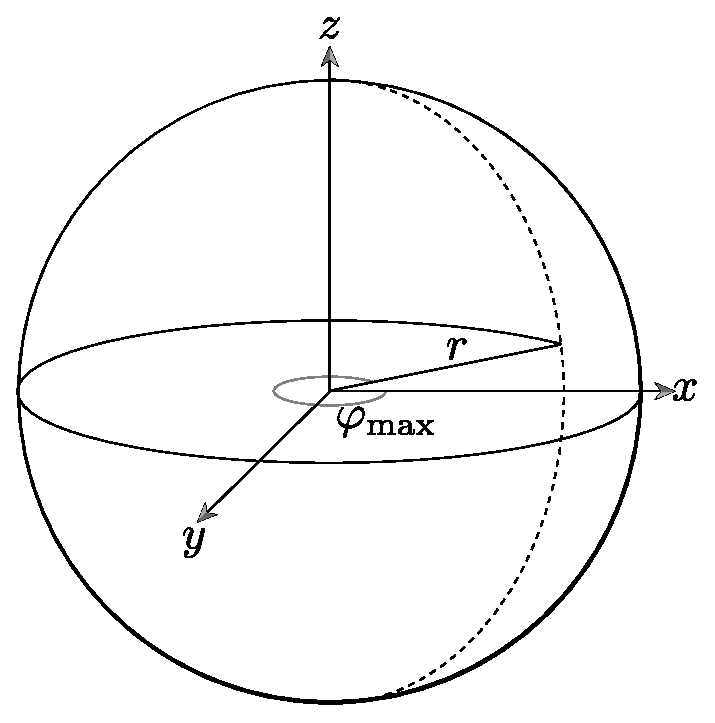
\includegraphics[width=0.35\linewidth]{chap03/Spheresetting.eps}
    \caption{球体形状基本设置。它半径为$r$,球心位于物体空间原点。
        部分球体可以通过指定$\varphi$的最大值描述。}
    \label{fig:3.4}
\end{figure}

我们可以用以下替换将该函数$f(\theta,\varphi)$转换为$[0,1]^2$上的函数$f(u,v)$并
稍微将其一般化以允许部分球体只扫过$\theta\in[\theta_{\min},\theta_{\max}]$和$\varphi\in[0,\varphi_{\max}]$:
\begin{align*}
    \varphi & =u\varphi_{\max}\, ,                              \\
    \theta  & =\theta_{\min}+v(\theta_{\max}-\theta_{\min})\, .
\end{align*}

该形式对纹理贴图特别有用,它能直接用来
将定义在$[0,1]^2$上的纹理映射到球上。
\reffig{3.5}展示了两个球的一张图像;一张网格图像用于展示$(u,v)$参数化。
\begin{figure}[htbp]
    \centering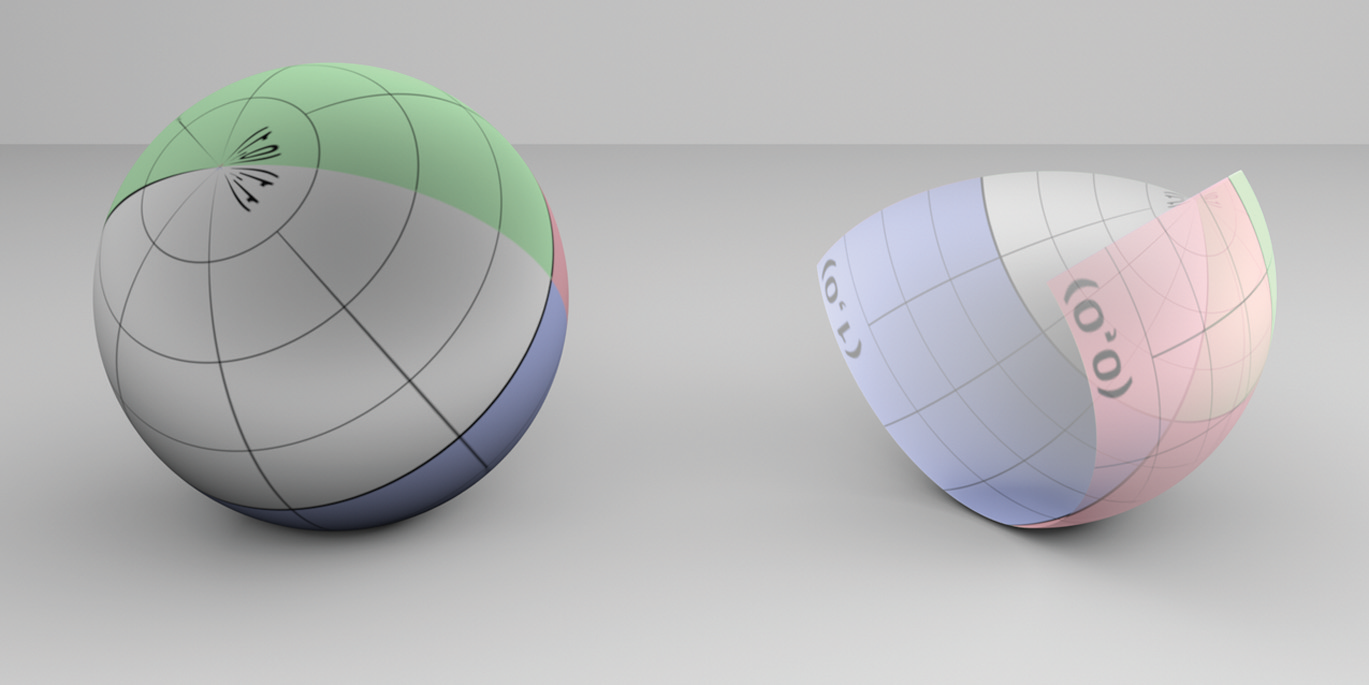
\includegraphics[width=\linewidth]{chap03/twospheres.png}
    \caption{两个球。左边是完整球,右边是部分球($z_{\max}<r$和$\varphi_{\max}<2\pi$)。
        注意纹理贴图用来展示形状$(u,v)$参数化;一极的\protect\keyindex{奇点}{singularity}{}在完整球中可见。}
    \label{fig:3.5}
\end{figure}

当我们描述球形状的实现时,我们将同时利用形状的隐式和参数化描述,
这取决于哪种方式能更自然地解决我们面临的特定问题。

类\refvar{Sphere}{}表示球心在物体空间原点的球体。
其实现在\href{https://github.com/mmp/pbrt-v3/tree/master/src/shapes/sphere.h}{\ttfamily shapes/sphere.h}
和\href{https://github.com/mmp/pbrt-v3/tree/master/src/shapes/sphere.cpp}{\ttfamily shapes/sphere.cpp}文件中。
\begin{lstlisting}
`\initcode{Sphere Declarations}{=}`
class `\initvar{Sphere}{}` : public `\refvar{Shape}{}` {
public:
    `\refcode{Sphere Public Methods}{}`
private:
    `\refcode{Sphere Private Data}{}`
};
\end{lstlisting}

为了在场景中别处放置球体,用户在输入文件里指定球体时必须施加合适的变换。
它同时接收物体到世界和世界到物体的变换作为参数给构造函数,
并将它们传给父类\refvar{Shape}{}的构造函数。

球的半径可以是任意正值,且球的范围可用两种方式截断。
第一,设置最小和最大$z$值;球体分别位于这些平面之下和之上的部分会被切除。
第二,在球面坐标中考虑球的参数化,可设置最大的$\varphi$值。
球体的$\varphi$值扫过从$0$到给定$\varphi_{\max}$的范围,
这样超出$\varphi_{\max}$的$\varphi$值对应的球体部分也被移除。
\begin{lstlisting}
`\initcode{Sphere Public Methods}{=}`
`\refvar{Sphere}{}`(const `\refvar{Transform}{}` *ObjectToWorld, const `\refvar{Transform}{}` *WorldToObject,
       bool reverseOrientation, `\refvar{Float}{}` radius, `\refvar{Float}{}` zMin, `\refvar{Float}{}` zMax,
       `\refvar{Float}{}` phiMax)
    : `\refvar{Shape}{}`(ObjectToWorld, WorldToObject, reverseOrientation),
      `\refvar[Sphere::radius]{radius}{}`(radius), `\refvar[Sphere::zMin]{zMin}{}`(`\refvar{Clamp}{}`(std::min(zMin, zMax), -radius, radius)),
      `\refvar[Sphere::zMax]{zMax}{}`(`\refvar{Clamp}{}`(std::max(zMin, zMax), -radius, radius)),
      `\refvar[Sphere::thetaMin]{thetaMin}{}`(std::acos(`\refvar{Clamp}{}`(zMin / radius, -1, 1))),
      `\refvar[Sphere::thetaMax]{thetaMax}{}`(std::acos(`\refvar{Clamp}{}`(zMax / radius, -1, 1))),
      `\refvar[Sphere::phiMax]{phiMax}{}`(`\refvar{Radians}{}`(`\refvar{Clamp}{}`(phiMax, 0, 360))) { }
\end{lstlisting}
\begin{lstlisting}
`\initcode{Sphere Private Data}{=}`
const `\refvar{Float}{}` `\initvar[Sphere::radius]{radius}{}`;
const `\refvar{Float}{}` `\initvar[Sphere::zMin]{zMin}{}`, `\initvar[Sphere::zMax]{zMax}{}`;
const `\refvar{Float}{}` `\initvar[Sphere::thetaMin]{thetaMin}{}`, `\initvar[Sphere::thetaMax]{thetaMax}{}`, `\initvar[Sphere::phiMax]{phiMax}{}`;
\end{lstlisting}

\subsection{边界}\label{sub:边界2}
计算球体的物体空间边界框很简单。
当要渲染的部分少于整个球体时,这里的实现使用用户提供的$z_{\min}$和$z_{\max}$值来缩紧边界。
然而,当$\varphi_{\max}$少于$\displaystyle\frac{3\pi}{2}$时它并不做额外工作计算更紧的边界框。
该改进留作习题。
\begin{lstlisting}
`\initcode{Sphere Method Definitions}{=}\initnext{SphereMethodDefinitions}`
`\refvar{Bounds3f}{}` `\refvar{Sphere}{}`::`\initvar[Sphere::ObjectBound]{\refvar{ObjectBound}{}}{}`() const {
    return `\refvar{Bounds3f}{}`(`\refvar{Point3f}{}`(-`\refvar[Sphere::radius]{radius}{}`, -`\refvar[Sphere::radius]{radius}{}`, `\refvar[Sphere::zMin]{zMin}{}`),
                    `\refvar{Point3f}{}`( `\refvar[Sphere::radius]{radius}{}`,  `\refvar[Sphere::radius]{radius}{}`, `\refvar[Sphere::zMax]{zMax}{}`));
}
\end{lstlisting}

\subsection{相交测试}\label{sub:相交测试2}
推导光线-球体相交测试的任务被球心位于原点的事实简化了。
然而如果球已被变换到世界空间的另一位置,
则光线与球相交前需要用世界到物体的变换来变到物体空间。
有了物体空间的光线,就能在物体空间执行相交计算了
\footnote{这是计算机图形学的经典主题。
    通过把问题转换为特定受限的情况,就可能更简单高效地做相交测试:
    即因为球总是在$(0,0,0)$,方程的许多项就消掉了。
    这不会失去一般性,因为对于其他位置的球体,适当平移光线即可。}。

下列代码片展示了整个相交方法:
\begin{lstlisting}
`\refcode{Sphere Method Definitions}{+=}\lastnext{SphereMethodDefinitions}`
bool `\refvar{Sphere}{}`::`\initvar[Sphere::Intersect]{\refvar[Shape::Intersect]{Intersect}{}}{}`(const `\refvar{Ray}{}` &r, `\refvar{Float}{}` *tHit,
        `\refvar{SurfaceInteraction}{}` *isect, bool testAlphaTexture) const {
    `\refvar{Float}{}` phi;
    `\refvar{Point3f}{}` pHit;
    `\refcode{Transform Ray to object space}{}`
    `\refcode{Compute quadratic sphere coefficients}{}`
    `\refcode{Solve quadratic equation for t values}{}`
    `\refcode{Compute sphere hit position and $\varphi$}{}`
    `\refcode{Test sphere intersection against clipping parameters}{}`
    `\refcode{Find parametric representation of sphere hit}{}`
    `\refcode{Compute error bounds for sphere intersection}{}`
    `\refcode{Initialize SurfaceInteraction from parametric information}{}`
    `\refcode{Update tHit for quadric intersection}{}`
    return true;
}
\end{lstlisting}

首先,所给世界空间光线被变换到球的物体空间。
相交测试的剩余部分将在那个坐标系内进行。
{\ttfamily oErr}和{\ttfamily dErr}变量分别定界
在变换射线端点和方向时因为施加变换而引入的浮点舍入误差
(更多关于浮点算术和其对于准确光线相交计算实现的更多信息见\refsec{控制舍入误差})。
\begin{lstlisting}
`\initcode{Transform Ray to object space}{=}`
`\refvar{Vector3f}{}` oErr, dErr;
`\refvar{Ray}{}` ray = (*`\refvar{WorldToObject}{}`)(r, &oErr, &dErr);
\end{lstlisting}

如果球心在原点,半径为$r$,则其隐式表示是
\begin{align*}
    x^2+y^2+z^2-r^2=0\, .
\end{align*}

通过将\refeq{2.3}中射线的参数表示代入隐式球方程,我们有
\begin{align*}
    (o_x+td_x)^2+(o_y+td_y)^2+(o_z+td_z)^2=r^2\, .
\end{align*}

注意该方程除了$t$的所有元素都是已知量。
使方程成立的$t$值给出了光线上使隐式球方程成立的参数化位置,
即沿光线与球相交的点。
我们可以展开该方程并整理系数得到$t$的一般二次方程,
\begin{align*}
    at^2+bt+c=0\, ,
\end{align*}
其中\footnote{一些光线追踪器要求规范化射线方向向量,即$a=1$。
    然而如果调用者忘记规范化射线方向则会导致微妙错误。
    当然,该错误可以通过在射线构造函数内规范化方向来避免,
    但这在提供的方向\emph{已经}规范化时会浪费精力。
    为了避免这无用的复杂性,pbrt没有在相交例程中坚持向量规范化。
    这特别有用,因为它减少了将射线变换到物体空间所需的计算量,即不需要规范化。}
\begin{align*}
    a & =d_x^2+d_y^2+d_z^2\, ,       \\
    b & =2(d_xo_x+d_yo_y+d_zo_z)\, , \\
    c & =o_x^2+o_y^2+o_z^2-r^2\, .
\end{align*}

该结果可以直接翻译为源码片。注意在该代码中,
类\refvar{EFloat}{}的而不是\refvar{Float}{}
的实例用于表示浮点值。\refvar{EFloat}{}跟踪累积的浮点舍入误差;
\refsec{控制舍入误差}将讨论它的使用。
至于现在,阅读时可以认为它和\refvar{Float}{}等价。
\begin{lstlisting}
`\initcode{Compute quadratic sphere coefficients}{=}`
`\refcode{Initialize EFloat ray coordinate values}{}`
`\refvar{EFloat}{}` a = dx * dx + dy * dy + dz * dz;
`\refvar{EFloat}{}` b = 2 * (dx * ox + dy * oy + dz * oz);
`\refvar{EFloat}{}` c = ox * ox + oy * oy + oz * oz - `\refvar{EFloat}{}`(`\refvar[Sphere::radius]{radius}{}`) * `\refvar{EFloat}{}`(`\refvar[Sphere::radius]{radius}{}`);
\end{lstlisting}

相交测试用的射线端点和方向值由将射线变换到物体空间的浮点误差界初始化。
\begin{lstlisting}
`\initcode{Initialize EFloat ray coordinate values}{=}`
`\refvar{EFloat}{}` ox(ray.o.x, oErr.x), oy(ray.o.y, oErr.y), oz(ray.o.z, oErr.z);
`\refvar{EFloat}{}` dx(ray.d.x, dErr.x), dy(ray.d.y, dErr.y), dz(ray.d.z, dErr.z);
\end{lstlisting}

二次方程有两个可能的解,给出光线交于球体的零、一或两个非虚数$t$值。
\begin{lstlisting}
`\initcode{Solve quadratic equation for t values}{=}`
`\refvar{EFloat}{}` t0, t1;
if (!`\refvar{Quadratic}{}`(a, b, c, &t0, &t1))
    return false;
`\refcode{Check quadric shape t0 and t1 for nearest intersection}{}`
\end{lstlisting}

实用函数\refvar{Quadratic}{}求解二次方程,
如果没有实数解就返回{\ttfamily false},
如果有则返回{\ttfamily true}并适当设置{\ttfamily t0}和{\ttfamily t1}。
稍后将在\refsub{求解二次方程}\sidenote{译者注:原文此处似乎链接章节错误,已修正。}定义它,
我们会讨论怎样用浮点算术稳定地实现它。

算得的参数化距离{\ttfamily t0}和{\ttfamily t1}跟踪了
原始射线参数的误差和\refvar{Quadratic}{}内累积的误差造成的不确定性;
不确定性区间范围的下界和上界可以使用方法\refvar[LowerBound]{EFloat::LowerBound}{()}和
\refvar[UpperBound]{EFloat::UpperBound}{()}获取。

代码片\refcode{Check quadric shape t0 and t1 for nearest intersection}{}取
两个相交值并确定如果有的话哪一个是最近的有效相交处。
对于有效的相交处,其值必须大于零且小于{\ttfamily ray.\refvar{tMax}{}}。
下列代码使用类\refvar{EFloat}{}提供的误差区间并只接受
明确在范围$(0,$\refvar{tMax}{}$)$内的相交处。

因为$t_0$保证小于或等于$t_1$(且$0$小于\refvar{tMax}{}),
则如果$t_0$大于\refvar{tMax}{}或$t_1$小于$0$,
那么两个相交处都一定超出了考虑范围。
否则,$t_0$是暂时的命中$t$值。
但它可能小于$0$,这时我们忽略它并尝试$t_1$。
如果也超出范围,我们就没有有效相交处。
如果有一个相交处,则初始化{\ttfamily tShapeHit}来保存该相交处的参数$t$值。
\begin{lstlisting}
`\initcode{Check quadric shape t0 and t1 for nearest intersection}{=}`
if (t0.`\refvar{UpperBound}{}`() > ray.`\refvar{tMax}{}` || t1.`\refvar{LowerBound}{}`() <= 0)
    return false;
`\refvar{EFloat}{}` tShapeHit = t0;
if (tShapeHit.`\refvar{LowerBound}{}`() <= 0) {
    tShapeHit = t1;
    if (tShapeHit.`\refvar{UpperBound}{}`() > ray.`\refvar{tMax}{}`)
        return false;
}
\end{lstlisting}
有了射线与完整球体相交的参数距离,
就能按沿射线的偏移量计算交点{\ttfamily pHit}。

接下来需要处理带有截断$z$或$\varphi$范围的部分球体——
必须忽略与截去区域的相交。
实现从计算命中点的$\varphi$值开始。使用球的参数化表示,
\begin{align*}
    \frac{y}{x}=\frac{r\sin\theta\sin\varphi}{r\sin\theta\cos\varphi}=\tan\varphi\, ,
\end{align*}
所以$\displaystyle\varphi=\arctan\frac{y}{x}$。
为了符合球的原始定义,需要将标准库函数{\ttfamily std::atan()}的
结果重新映射为$0$到$2\pi$的值。
\begin{lstlisting}
`\initcode{Compute sphere hit position and $\varphi$}{=}`
pHit = ray((`\refvar{Float}{}`)tShapeHit);
`\refcode{Refine sphere intersection point}{}`
if (pHit.x == 0 && pHit.y == 0) pHit.x = 1e-5f * `\refvar[Sphere::radius]{radius}{}`;
phi = std::atan2(pHit.y, pHit.x);
if (phi < 0) phi += 2 * `\refvar{Pi}{}`;
\end{lstlisting}

由于浮点精度限制,算得的该交点{\ttfamily pHit}可能位于实际球体表面的一侧;
定义于\refsub{定界交点误差}的
代码片\refcode{Refine sphere intersection point}{}会提升该值精度。

现在可以针对$z$和$\varphi$指定的最小值和最大值测试命中点了。
一个细节是如果$z$范围包括了整个球体则跳过$z$测试非常重要;
算得的值{\ttfamily pHit.z}可能因为浮点舍入超出$z$范围一点点,
所以我们应该只在用户希望球体是部分不完整时才执行该测试。
如果$t_0$相交处实际无效,例程就再次尝试$t_1$。
\begin{lstlisting}
`\initcode{Test sphere intersection against clipping parameters}{=}`
if ((`\refvar[Sphere::zMin]{zMin}{}` > -`\refvar[Sphere::radius]{radius}{}` && pHit.z < `\refvar[Sphere::zMin]{zMin}{}`) ||
    (`\refvar[Sphere::zMax]{zMax}{}` <  `\refvar[Sphere::radius]{radius}{}` && pHit.z > `\refvar[Sphere::zMax]{zMax}{}`) || phi > `\refvar[Sphere::phiMax]{phiMax}{}`) {
    if (tShapeHit == t1) return false;
    if (t1.`\refvar{UpperBound}{}`() > ray.`\refvar{tMax}{}`) return false;
    tShapeHit = t1;
    `\refcode{Compute sphere hit position and $\varphi$}{}`
    if ((`\refvar[Sphere::zMin]{zMin}{}` > -`\refvar[Sphere::radius]{radius}{}` && pHit.z < `\refvar[Sphere::zMin]{zMin}{}`) ||
        (`\refvar[Sphere::zMax]{zMax}{}` <  `\refvar[Sphere::radius]{radius}{}` && pHit.z > `\refvar[Sphere::zMax]{zMax}{}`) || phi > `\refvar[Sphere::phiMax]{phiMax}{}`)
        return false;
}
\end{lstlisting}

在例程中的此处,光线一定命中了球体。
接下来方法分别通过缩放之前计算的$\varphi$值来为命中点计算在0到1之间的$u$值,
并基于所给球体的$\theta$值范围通过为命中点计算0到1的$\theta$值来计算$v$值
\sidenote{译者注:这句话太绕了,我投降,请大佬赐教怎么翻译。
    看不懂没关系,去翻翻前面$u,v$与$\varphi,\theta$的关系你就懂了。}。
然后它再求位置的参数化偏导数$\displaystyle\frac{\partial \bm p}{\partial u}$和
$\displaystyle\frac{\partial \bm p}{\partial v}$以及
曲面法线的$\displaystyle\frac{\partial \bm n}{\partial u}$和
$\displaystyle\frac{\partial \bm n}{\partial v}$。
\begin{lstlisting}
`\initcode{Find parametric representation of sphere hit}{=}`
`\refvar{Float}{}` u = phi / `\refvar[Sphere::phiMax]{phiMax}{}`;
`\refvar{Float}{}` theta = std::acos(`\refvar{Clamp}{}`(pHit.z / `\refvar[Sphere::radius]{radius}{}`, -1, 1));
`\refvar{Float}{}` v = (theta - `\refvar[Sphere::thetaMin]{thetaMin}{}`) / (`\refvar[Sphere::thetaMax]{thetaMax}{}` - `\refvar[Sphere::thetaMin]{thetaMin}{}`);
`\refcode{Compute sphere $\partial$p/$\partial$u and $\partial$p/$\partial$v}{}`
`\refcode{Compute sphere $\partial$n/$\partial$u and $\partial$n/$\partial$v}{}`
\end{lstlisting}

计算球上一点的偏导数是个代数小习题。
这里我们将展示怎样计算$\displaystyle\frac{\partial \bm p}{\partial u}$的$x$分量,
$\displaystyle\frac{\partial p_x}{\partial u}$;
其他分量解法相同。使用球的参数化定义,我们有\sidenote{译者注:这里$p_x$与$x$含义相同,以此类推。}
\begin{align*}
    x                               & =r\sin\theta\cos\varphi\, ,                          \\
    \frac{\partial p_x}{\partial u} & =\frac{\partial}{\partial u}(r\sin\theta\cos\varphi) \\
                                    & =r\sin\theta\frac{\partial\cos\varphi}{\partial u}   \\
                                    & =-r\varphi_{\max}\sin\theta\sin\varphi\, .
\end{align*}

基于球$y$坐标的参数化定义进行代换,可以简化为
\begin{align*}
    \frac{\partial p_x}{\partial u}=-\varphi_{\max}y\, .
\end{align*}
同样
\begin{align*}
    \frac{\partial p_y}{\partial u}=\varphi_{\max}x\, ,
\end{align*}
以及
\begin{align*}
    \frac{\partial p_z}{\partial u}=0\, .
\end{align*}

同样过程求得$\displaystyle\frac{\partial \bm p}{\partial v}$,完整结果为
\begin{align*}
    \frac{\partial \bm p}{\partial u} & =(-\varphi_{\max}y,\varphi_{\max}x,0)\, ,                                  \\
    \frac{\partial \bm p}{\partial v} & =(\theta_{\max}-\theta_{\min})(z\cos\varphi,z\sin\varphi,-r\sin\theta)\, .
\end{align*}
\begin{lstlisting}
`\initcode{Compute sphere $\partial$p/$\partial$u and $\partial$p/$\partial$v}{=}`
`\refvar{Float}{}` zRadius = std::sqrt(pHit.x * pHit.x + pHit.y * pHit.y);
`\refvar{Float}{}` invZRadius = 1 / zRadius;
`\refvar{Float}{}` cosPhi = pHit.x * invZRadius;
`\refvar{Float}{}` sinPhi = pHit.y * invZRadius;
`\refvar{Vector3f}{}` dpdu(-`\refvar[Sphere::phiMax]{phiMax}{}` * pHit.y, `\refvar[Sphere::phiMax]{phiMax}{}` * pHit.x, 0);
`\refvar{Vector3f}{}` dpdv = (`\refvar[Sphere::thetaMax]{thetaMax}{}` - `\refvar[Sphere::thetaMin]{thetaMin}{}`) *
    `\refvar{Vector3f}{}`(pHit.z * cosPhi, pHit.z * sinPhi,
             -`\refvar[Sphere::radius]{radius}{}` * std::sin(theta));
\end{lstlisting}

\subsection{法向量的偏导数}\label{sub:法向量的偏导数}
\begin{remark}
    本节含有高级内容,第一次阅读时可以跳过。
\end{remark}

当我们沿表面在$u$和$v$方向移动时,确定法线是怎样变化的也很有用。
例如,第\refchap{纹理}的抗锯齿技术就依赖于该信息来消除物体曲面上反射可见的纹理锯齿。
法线的微分变化量$\displaystyle\frac{\partial \bm n}{\partial u}$和
$\displaystyle\frac{\partial \bm n}{\partial v}$由微分几何学
中\keyindex{曲面的外恩加滕公式}{Weingarten formula of surfaces}{surface曲面}给出
\sidenote{译者注:得名于德国数学家Julius Weingarten。
    相关简要推导详见译者整理补充的\refsec{译者补充:微分几何基础}。
    注意该公式其实隐含了对$\bm n$的规范化要求。
    下面所提的第一基本形式、第二基本形式也是微分几何学中的概念。}:
\begin{align*}
    \frac{\partial \bm n}{\partial u} & =\frac{fF-eG}{EG-F^2}\frac{\partial \bm p}{\partial u}+\frac{eF-fE}{EG-F^2}\frac{\partial \bm p}{\partial v}\, , \\
    \frac{\partial \bm n}{\partial v} & =\frac{gF-fG}{EG-F^2}\frac{\partial \bm p}{\partial u}+\frac{fF-gE}{EG-F^2}\frac{\partial \bm p}{\partial v}\, ,
\end{align*}
其中$E,F$和$G$是\keyindex{第一基本形式}{the first fundamental form}{}的系数,即
\begin{align*}
    E & =\left|\frac{\partial \bm p}{\partial u}\right|^2\, ,                                     \\
    F & =\left(\frac{\partial \bm p}{\partial u}\cdot\frac{\partial \bm p}{\partial v}\right)\, , \\
    G & =\left|\frac{\partial \bm p}{\partial v}\right|^2\, .
\end{align*}

它们可以利用之前算得的$\displaystyle\frac{\partial \bm p}{\partial u}$和$\displaystyle\frac{\partial \bm p}{\partial v}$轻松算出。
$e,f$和$g$是\keyindex{第二基本形式}{the second fundamental form}{}的系数,
\begin{align*}
    e & =\left(\bm n\cdot\frac{\partial^2\bm p}{\partial u^2}\right)\, ,         \\
    f & =\left(\bm n\cdot\frac{\partial^2\bm p}{\partial u\partial v}\right)\, , \\
    g & =\left(\bm n\cdot\frac{\partial^2\bm p}{\partial v^2}\right)\, .
\end{align*}

两个基本形式刻画了曲面的基本度量属性,包括距离、角度和\keyindex{曲率}{curvature}{}的概念;
细节详见微分几何教材例如\citet{gray2017modern}
\sidenote{译者注:此处引用文献改为了新版。}。
为了求$e,f$和$g$,需要计算二阶偏导数$\displaystyle\frac{\partial^2\bm p}{\partial u^2}$等。

对于球体,可以算得二阶导数为:
\begin{align*}
    \frac{\partial^2\bm p}{\partial u^2}         & =-\varphi_{\max}^2(x,y,0)\, ,                                                 \\
    \frac{\partial^2\bm p}{\partial u\partial v} & =(\theta_{\max}-\theta_{\min})z\varphi_{\max}(-\sin\varphi,\cos\varphi,0)\, , \\
    \frac{\partial^2\bm p}{\partial v^2}         & =-(\theta_{\max}-\theta_{\min})^2(x,y,z)\, .
\end{align*}
\begin{lstlisting}
`\initcode{Compute sphere $\partial$n/$\partial$u and $\partial$n/$\partial$v}{=}`
`\refvar{Vector3f}{}` d2Pduu = -`\refvar[Sphere::phiMax]{phiMax}{}` * `\refvar[Sphere::phiMax]{phiMax}{}` * `\refvar{Vector3f}{}`(pHit.x, pHit.y, 0);
`\refvar{Vector3f}{}` d2Pduv = (`\refvar[Sphere::thetaMax]{thetaMax}{}` - `\refvar[Sphere::thetaMin]{thetaMin}{}`) * pHit.z * `\refvar[Sphere::phiMax]{phiMax}{}` *
                  `\refvar{Vector3f}{}`(-sinPhi, cosPhi, 0.);
`\refvar{Vector3f}{}` d2Pdvv = -(`\refvar[Sphere::thetaMax]{thetaMax}{}` - `\refvar[Sphere::thetaMin]{thetaMin}{}`) * (`\refvar[Sphere::thetaMax]{thetaMax}{}` - `\refvar[Sphere::thetaMin]{thetaMin}{}`) *
                  `\refvar{Vector3f}{}`(pHit.x, pHit.y, pHit.z);
`\refcode{Compute coefficients for fundamental forms}{}`
`\refcode{Compute $\partial$n/$\partial$u and $\partial$n/$\partial$v from fundamental form coefficients}{}`
\end{lstlisting}
\begin{lstlisting}
`\initcode{Compute coefficients for fundamental forms}{=}`
`\refvar{Float}{}` E = `\refvar{Dot}{}`(dpdu, dpdu);
`\refvar{Float}{}` F = `\refvar{Dot}{}`(dpdu, dpdv);
`\refvar{Float}{}` G = `\refvar{Dot}{}`(dpdv, dpdv);
`\refvar{Vector3f}{}` N = `\refvar{Normalize}{}`(`\refvar{Cross}{}`(dpdu, dpdv));
`\refvar{Float}{}` e = `\refvar{Dot}{}`(N, d2Pduu);
`\refvar{Float}{}` f = `\refvar{Dot}{}`(N, d2Pduv);
`\refvar{Float}{}` g = `\refvar{Dot}{}`(N, d2Pdvv);
\end{lstlisting}
\begin{lstlisting}
`\initcode{Compute $\partial$n/$\partial$u and $\partial$n/$\partial$v from fundamental form coefficients}{=}`
`\refvar{Float}{}` invEGF2 = 1 / (E * G - F * F);
`\refvar{Normal3f}{}` dndu = `\refvar{Normal3f}{}`((f * F - e * G) * invEGF2 * dpdu + 
                         (e * F - f * E) * invEGF2 * dpdv);
`\refvar{Normal3f}{}` dndv = `\refvar{Normal3f}{}`((g * F - f * G) * invEGF2 * dpdu + 
                         (f * F - g * E) * invEGF2 * dpdv);
\end{lstlisting}

\subsection{SurfaceInteraction 初始化}
计算了曲面参数化和所有相关偏导数后,
可以用该相交处的几何信息初始化结构\refvar{SurfaceInteraction}{}了。
传给\refvar{SurfaceInteraction}{}构造函数的\refvar{pError}{}值
定界了算得的点{\ttfamily pHit}中的舍入误差。
它在稍后于\refsub{定界交点误差}定义的代码片\refcode{Compute error bounds for sphere intersection}{}中初始化。
\begin{lstlisting}
`\initcode{Initialize SurfaceInteraction from parametric information}{=}`
*isect = (*`\refvar{ObjectToWorld}{}`)(
    `\refvar{SurfaceInteraction}{}`(pHit, `\refvar{pError}{}`, `\refvar{Point2f}{}`(u, v), -ray.`\refvar[Ray::d]{d}{}`, dpdu, dpdv,
                       dndu, dndv, ray.`\refvar[Ray::time]{time}{}`, this));
\end{lstlisting}

因为有相交处,已存于{\ttfamily tShapeHit}的光线上的命中参数距离将更新
方法\refvar[Shape::Intersect]{Intersect}{}的参数{\ttfamily tHit}。
如果可能的命中点比已有的相交处更远,则更新{\ttfamily *tHit}能让后续相交测试提前终止。
\begin{lstlisting}
`\initcode{Update tHit for quadric intersection}{=}`
*tHit = (`\refvar{Float}{}`)tShapeHit;
\end{lstlisting}

这里自然会问道:“世界到物体变换对于返回正确的参数距离有何影响呢?”
确实,相交方法已经为物体空间射线求得到相交处的参数距离,
它可能已被平移、旋转、缩放,甚至是从世界空间变换来的。
然而,可以证明在物体空间内到相交处的参数距离正好等于
把射线留在世界空间内并在那里求相交后得到的距离,
因此,{\ttfamily *tHit}可以直接设置。
注意如果物体空间射线的方向在变换后被规范化,那就不是这种情况了,
会需要一个与未规范化射线的长度相关的校正因子。
这是变换后不规范化物体空间射线方向向量的另一个动机。

\refvar{Sphere::IntersectP}{()}例程几乎和\refvar{Sphere::Intersect}{()}一样,
但它不初始化结构\refvar{SurfaceInteraction}{}。
因为方法\refvar[Shape::Intersect]{Intersect}{}和\refvar[Shape::IntersectP]{IntersectP}{()}总是如此接近,
接下来我们不再为剩余形状展示\refvar[Shape::IntersectP]{IntersectP}{()}。
\begin{lstlisting}
`\refcode{Sphere Method Definitions}{+=}\lastnext{SphereMethodDefinitions}`
bool `\refvar{Sphere}{}`::`\initvar[Sphere::IntersectP]{\refvar[Shape::IntersectP]{IntersectP}{}}{}`(const `\refvar{Ray}{}` &r, bool testAlphaTexture) const {
    `\refvar{Float}{}` phi;
    `\refvar{Point3f}{}` pHit;
    `\refcode{Transform Ray to object space}{}`
    `\refcode{Compute quadratic sphere coefficients}{}`
    `\refcode{Solve quadratic equation for t values}{}`
    `\refcode{Compute sphere hit position and $\varphi$}{}`
    `\refcode{Test sphere intersection against clipping parameters}{}`
    return true;
}
\end{lstlisting}

\subsection{表面积}\label{sub:表面积2}
为了计算二次曲面的表面积,我们使用\keyindex{积分学}{integral calculus}{}的标准公式。
如果定义于$x=a$到$x=b$的\keyindex{曲线}{curve}{}$y=f(x)$绕$x$轴旋转,
则所得扫掠曲面的表面积为
\begin{align*}
    2\pi\int_a^b{f(x)\sqrt{1+(f'(x))^2}\mathrm{d}x}\, ,
\end{align*}
其中$f'(x)$表示导数$\displaystyle\frac{\mathrm{d}f}{\mathrm{d}x}$。
因为我们大多数的旋转表面都只是绕轴部分扫掠的,所以我们替代使用公式
\begin{align*}
    \varphi_{\max}\int_a^b{f(x)\sqrt{1+(f'(x))^2}\mathrm{d}x}\, .
\end{align*}

球面是\keyindex{圆弧}{circular arc}{}旋转的曲面。
沿球体$z$轴定义轮廓曲线的函数是
\begin{align*}
    f(z)=\sqrt{r^2-z^2}\, ,
\end{align*}
并且其导数为
\begin{align*}
    f'(z)=-\frac{z}{\sqrt{r^2-z^2}}\, .
\end{align*}

回想球体在$z_{\min}$和$z_{\max}$处被裁剪。因此表面积为
\begin{align*}
    A & =\varphi_{\max}\int_{z_{\min}}^{z_{\max}}{\sqrt{r^2-z^2}\sqrt{1+\frac{z^2}{r^2-z^2}}\mathrm{d}z} \\
      & =\varphi_{\max}\int_{z_{\min}}^{z_{\max}}{\sqrt{r^2-z^2+z^2}\mathrm{d}z}                         \\
      & =\varphi_{\max}\int_{z_{\min}}^{z_{\max}}{r\mathrm{d}z}                                          \\
      & =\varphi_{\max}r(z_{\max}-z_{\min})\, .
\end{align*}

对于完整球体$\varphi_{\max}=2\pi$,$z_{\min}=-r$且$z_{\max}=r$,
所以我们有标准公式$A=4\pi r^2$,确认该公式有意义。
\begin{lstlisting}
`\refcode{Sphere Method Definitions}{+=}\lastnext{SphereMethodDefinitions}`
`\refvar{Float}{}` `\refvar{Sphere}{}`::`\initvar[Sphere::Area]{\refvar[Shape::Area]{Area}{}}{}`() const {
    return `\refvar[Sphere::phiMax]{phiMax}{}` * `\refvar[Sphere::radius]{radius}{}` * (`\refvar[Sphere::zMax]{zMax}{}` - `\refvar[Sphere::zMin]{zMin}{}`);
}
\end{lstlisting}

\section{圆柱体}\label{sec:圆柱体}

另一个有用的二次曲面是\keyindex{圆柱体}{cylinder}{};
pbrt提供以$z$轴为中心的圆柱体\refvar{Shape}{}。
实现在文件\href{https://github.com/mmp/pbrt-v3/tree/master/src/shapes/cylinder.h}{\ttfamily shapes/cylinder.h}和
\href{https://github.com/mmp/pbrt-v3/tree/master/src/shapes/cylinder.cpp}{\ttfamily shapes/cylinder.cpp}内。
用户为圆柱体提供最小和最大$z$值,以及半径和最大扫掠值$\varphi$(\reffig{3.6})。
\begin{figure}[htbp]
    \centering%LaTeX with PSTricks extensions
%%Creator: Inkscape 1.0.1 (3bc2e813f5, 2020-09-07)
%%Please note this file requires PSTricks extensions
\psset{xunit=.35pt,yunit=.35pt,runit=.35pt}
\begin{pspicture}(448.67001343,346.17999268)
{
\newrgbcolor{curcolor}{0.50196081 0.50196081 0.50196081}
\pscustom[linewidth=1,linecolor=curcolor]
{
\newpath
\moveto(247.69,277.90999268)
\curveto(247.69,272.81999268)(231.64,268.68999268)(211.84,268.68999268)
\curveto(192.04,268.68999268)(176,272.81999268)(176,277.90999268)
\curveto(176,282.99999268)(192.05,287.12999268)(211.84,287.12999268)
\curveto(222.98,287.12999268)(232.93,285.82999268)(239.5,283.77999268)
}
}
{
\newrgbcolor{curcolor}{0 0 0}
\pscustom[linewidth=1,linecolor=curcolor]
{
\newpath
\moveto(211.83000183,101.72999573)
\lineto(211.83000183,314.95999336)
}
}
{
\newrgbcolor{curcolor}{0 0 0}
\pscustom[linestyle=none,fillstyle=solid,fillcolor=curcolor]
{
\newpath
\moveto(217.34,310.04999268)
\lineto(211.83,314.30999268)
\lineto(206.33,310.04999268)
\lineto(211.83,323.05999268)
\closepath
}
}
{
\newrgbcolor{curcolor}{0.65098041 0.65098041 0.65098041}
\pscustom[linestyle=none,fillstyle=solid,fillcolor=curcolor]
{
\newpath
\moveto(216.13,311.60999268)
\lineto(211.83,321.74999268)
\lineto(211.83,314.93999268)
\closepath
}
}
{
\newrgbcolor{curcolor}{0.40000001 0.40000001 0.40000001}
\pscustom[linestyle=none,fillstyle=solid,fillcolor=curcolor]
{
\newpath
\moveto(207.53,311.60999268)
\lineto(211.83,321.74999268)
\lineto(211.83,314.93999268)
\closepath
}
}
{
\newrgbcolor{curcolor}{0 0 0}
\pscustom[linewidth=1,linecolor=curcolor]
{
\newpath
\moveto(211.83000183,102.07998657)
\lineto(132.74000549,23.97998047)
}
}
{
\newrgbcolor{curcolor}{0 0 0}
\pscustom[linestyle=none,fillstyle=solid,fillcolor=curcolor]
{
\newpath
\moveto(132.37,31.34999268)
\lineto(133.2,24.43999268)
\lineto(140.1,23.50999268)
\lineto(126.97,18.28999268)
\closepath
}
}
{
\newrgbcolor{curcolor}{0.65098041 0.65098041 0.65098041}
\pscustom[linestyle=none,fillstyle=solid,fillcolor=curcolor]
{
\newpath
\moveto(132.1,29.38999268)
\lineto(127.91,19.20999268)
\lineto(132.75,23.98999268)
\closepath
}
}
{
\newrgbcolor{curcolor}{0.40000001 0.40000001 0.40000001}
\pscustom[linestyle=none,fillstyle=solid,fillcolor=curcolor]
{
\newpath
\moveto(138.14,23.27999268)
\lineto(127.91,19.20999268)
\lineto(132.75,23.98999268)
\closepath
}
}
{
\newrgbcolor{curcolor}{0 0 0}
\pscustom[linewidth=1,linecolor=curcolor]
{
\newpath
\moveto(211.57000732,102.31999207)
\lineto(424.79998779,102.31999207)
}
}
{
\newrgbcolor{curcolor}{0 0 0}
\pscustom[linestyle=none,fillstyle=solid,fillcolor=curcolor]
{
\newpath
\moveto(419.89,96.80999268)
\lineto(424.15,102.31999268)
\lineto(419.89,107.81999268)
\lineto(432.91,102.31999268)
\closepath
}
}
{
\newrgbcolor{curcolor}{0.65098041 0.65098041 0.65098041}
\pscustom[linestyle=none,fillstyle=solid,fillcolor=curcolor]
{
\newpath
\moveto(421.45,98.01999268)
\lineto(431.59,102.31999268)
\lineto(424.78,102.31999268)
\closepath
}
}
{
\newrgbcolor{curcolor}{0.40000001 0.40000001 0.40000001}
\pscustom[linestyle=none,fillstyle=solid,fillcolor=curcolor]
{
\newpath
\moveto(421.45,106.61999268)
\lineto(431.59,102.31999268)
\lineto(424.78,102.31999268)
\closepath
}
}
{
\newrgbcolor{curcolor}{0 0 0}
\pscustom[linewidth=1,linecolor=curcolor]
{
\newpath
\moveto(350.83000183,277.73999023)
\curveto(350.83000183,286.35502645)(316.96111637,294.12183088)(265.01762877,297.41847591)
\curveto(213.07424711,300.71511422)(153.28645653,298.89232333)(113.53009079,292.80059904)
\curveto(73.77372505,286.70887475)(61.87766115,277.5478076)(83.39248224,269.58871089)
\curveto(104.90734722,261.62959795)(155.59577355,256.439991)(211.82000732,256.439991)
\curveto(268.0442411,256.439991)(318.73266743,261.62959795)(340.2475324,269.58871089)
\curveto(361.7623535,277.5478076)(349.86628959,286.70887475)(310.10992386,292.80059904)
\curveto(270.35355812,298.89232333)(210.56576754,300.71511422)(158.62238587,297.41847591)
\curveto(106.67889828,294.12183088)(72.81001282,286.35502645)(72.81001282,277.73999023)
\curveto(72.81001282,269.12495402)(106.67889828,261.35814959)(158.62238587,258.06150455)
\curveto(210.56576754,254.76486625)(270.35355812,256.58765714)(310.10992386,262.67938143)
\curveto(349.86628959,268.77110572)(361.7623535,277.93217287)(340.2475324,285.89126957)
\curveto(318.73266743,293.85038252)(268.0442411,299.03998947)(211.82000732,299.03998947)
\curveto(155.59577355,299.03998947)(104.90734722,293.85038252)(83.39248224,285.89126957)
\curveto(61.87766115,277.93217287)(73.77372505,268.77110572)(113.53009079,262.67938143)
\curveto(153.28645653,256.58765714)(213.07424711,254.76486625)(265.01762877,258.06150455)
\curveto(316.96111637,261.35814959)(350.83000183,269.12495402)(350.83000183,277.73999023)
\closepath
}
}
{
\newrgbcolor{curcolor}{0 0 0}
\pscustom[linewidth=1,linecolor=curcolor]
{
\newpath
\moveto(211.74000549,278.00999451)
\lineto(291.57000732,295.15999222)
}
}
{
\newrgbcolor{curcolor}{0 0 0}
\pscustom[linewidth=1,linecolor=curcolor]
{
\newpath
\moveto(211.88999939,278.00999451)
\lineto(350.79000854,278.00999451)
}
}
{
\newrgbcolor{curcolor}{0 0 0}
\pscustom[linewidth=1,linecolor=curcolor]
{
\newpath
\moveto(350.72999573,140.75)
\curveto(350.72999573,149.36503621)(316.86111027,157.13184065)(264.91762267,160.42848568)
\curveto(212.97424101,163.72512399)(153.18645043,161.90233309)(113.43008469,155.8106088)
\curveto(73.67371895,149.71888452)(61.77765504,140.55781737)(83.29247614,132.59872066)
\curveto(104.80734112,124.63960772)(155.49576745,119.45000076)(211.72000122,119.45000076)
\curveto(267.94423499,119.45000076)(318.63266133,124.63960772)(340.1475263,132.59872066)
\curveto(361.6623474,140.55781737)(349.76628349,149.71888452)(310.00991775,155.8106088)
\curveto(270.25355201,161.90233309)(210.46576143,163.72512399)(158.52237977,160.42848568)
\curveto(106.57889217,157.13184065)(72.71000671,149.36503621)(72.71000671,140.75)
\curveto(72.71000671,132.13496379)(106.57889217,124.36815935)(158.52237977,121.07151432)
\curveto(210.46576143,117.77487601)(270.25355201,119.59766691)(310.00991775,125.6893912)
\curveto(349.76628349,131.78111548)(361.6623474,140.94218263)(340.1475263,148.90127934)
\curveto(318.63266133,156.86039228)(267.94423499,162.04999924)(211.72000122,162.04999924)
\curveto(155.49576745,162.04999924)(104.80734112,156.86039228)(83.29247614,148.90127934)
\curveto(61.77765504,140.94218263)(73.67371895,131.78111548)(113.43008469,125.6893912)
\curveto(153.18645043,119.59766691)(212.97424101,117.77487601)(264.91762267,121.07151432)
\curveto(316.86111027,124.36815935)(350.72999573,132.13496379)(350.72999573,140.75)
\closepath
}
}
{
\newrgbcolor{curcolor}{0 0 0}
\pscustom[linewidth=1,linecolor=curcolor]
{
\newpath
\moveto(72.76999664,277.96999359)
\lineto(72.76999664,140.83999634)
}
}
{
\newrgbcolor{curcolor}{0 0 0}
\pscustom[linewidth=1,linecolor=curcolor]
{
\newpath
\moveto(350.79998779,278.11999512)
\lineto(350.79998779,140.22999573)
}
}
{
\newrgbcolor{curcolor}{0 0 0}
\pscustom[linewidth=1,linecolor=curcolor]
{
\newpath
\moveto(68.01000214,140.95999146)
\lineto(33.52000046,140.95999146)
}
}
{
\newrgbcolor{curcolor}{0 0 0}
\pscustom[linewidth=1,linecolor=curcolor]
{
\newpath
\moveto(68.01000214,277.78999329)
\lineto(33.52000046,277.78999329)
}
}
{
\newrgbcolor{curcolor}{0 0 0}
\pscustom[linestyle=none,fillstyle=solid,fillcolor=curcolor]
{
\newpath
\moveto(282.46993563,265.46999408)
\curveto(282.39181063,265.07936908)(282.23556063,264.49343158)(282.23556063,264.37624408)
\curveto(282.23556063,263.94655658)(282.58712313,263.71218158)(282.97774813,263.71218158)
\curveto(283.29024813,263.71218158)(283.71993563,263.90749408)(283.91524813,264.41530658)
\curveto(283.95431063,264.49343158)(284.77462313,267.89186908)(284.89181063,268.36061908)
\curveto(285.08712313,269.18093158)(285.55587313,270.89968158)(285.67306063,271.60280658)
\curveto(285.79024813,271.91530658)(286.49337313,273.08718158)(287.07931063,273.63405658)
\curveto(287.27462313,273.79030658)(288.01681063,274.45436908)(289.07149813,274.45436908)
\curveto(289.73556063,274.45436908)(290.08712313,274.14186908)(290.12618563,274.14186908)
\curveto(289.38399813,274.02468158)(288.83712313,273.43874408)(288.83712313,272.77468158)
\curveto(288.83712313,272.38405658)(289.11056063,271.91530658)(289.77462313,271.91530658)
\curveto(290.43868563,271.91530658)(291.14181063,272.50124408)(291.14181063,273.39968158)
\curveto(291.14181063,274.25905658)(290.36056063,275.00124408)(289.07149813,275.00124408)
\curveto(287.46993563,275.00124408)(286.37618563,273.79030658)(285.90743563,273.08718158)
\curveto(285.67306063,274.21999408)(284.77462313,275.00124408)(283.60274813,275.00124408)
\curveto(282.46993563,275.00124408)(282.00118563,274.02468158)(281.76681063,273.59499408)
\curveto(281.33712313,272.73561908)(281.02462313,271.25124408)(281.02462313,271.17311908)
\curveto(281.02462313,270.89968158)(281.25899813,270.89968158)(281.29806063,270.89968158)
\curveto(281.57149813,270.89968158)(281.57149813,270.93874408)(281.72774813,271.48561908)
\curveto(282.15743563,273.24343158)(282.66524813,274.45436908)(283.56368563,274.45436908)
\curveto(283.95431063,274.45436908)(284.30587313,274.25905658)(284.30587313,273.32155658)
\curveto(284.30587313,272.77468158)(284.22774813,272.50124408)(283.91524813,271.21218158)
\closepath
\moveto(282.46993563,265.46999408)
}
}
{
\newrgbcolor{curcolor}{0 0 0}
\pscustom[linestyle=none,fillstyle=solid,fillcolor=curcolor]
{
\newpath
\moveto(442.23157013,104.08531158)
\curveto(442.38782013,104.71031158)(442.97375763,107.01499908)(444.69250763,107.01499908)
\curveto(444.80969513,107.01499908)(445.43469513,107.01499908)(445.94250763,106.70249908)
\curveto(445.23938263,106.54624908)(444.77063263,105.96031158)(444.77063263,105.33531158)
\curveto(444.77063263,104.94468658)(445.04407013,104.47593658)(445.70813263,104.47593658)
\curveto(446.25500763,104.47593658)(447.03625763,104.90562408)(447.03625763,105.92124908)
\curveto(447.03625763,107.21031158)(445.59094513,107.56187408)(444.73157013,107.56187408)
\curveto(443.28625763,107.56187408)(442.42688263,106.23374908)(442.11438263,105.68687408)
\curveto(441.48938263,107.32749908)(440.16125763,107.56187408)(439.41907013,107.56187408)
\curveto(436.84094513,107.56187408)(435.39563263,104.35874908)(435.39563263,103.73374908)
\curveto(435.39563263,103.46031158)(435.66907013,103.46031158)(435.70813263,103.46031158)
\curveto(435.90344513,103.46031158)(435.98157013,103.53843658)(436.02063263,103.73374908)
\curveto(436.88000763,106.38999908)(438.52063263,107.01499908)(439.38000763,107.01499908)
\curveto(439.84875763,107.01499908)(440.70813263,106.78062408)(440.70813263,105.33531158)
\curveto(440.70813263,104.55406158)(440.27844513,102.91343658)(439.38000763,99.39781158)
\curveto(438.98938263,97.87437408)(438.09094513,96.81968658)(436.99719513,96.81968658)
\curveto(436.84094513,96.81968658)(436.29407013,96.81968658)(435.74719513,97.13218658)
\curveto(436.37219513,97.28843658)(436.91907013,97.79624908)(436.91907013,98.49937408)
\curveto(436.91907013,99.16343658)(436.37219513,99.35874908)(436.02063263,99.35874908)
\curveto(435.23938263,99.35874908)(434.65344513,98.73374908)(434.65344513,97.91343658)
\curveto(434.65344513,96.78062408)(435.86438263,96.27281158)(436.95813263,96.27281158)
\curveto(438.63782013,96.27281158)(439.53625763,98.03062408)(439.57532013,98.14781158)
\curveto(439.88782013,97.24937408)(440.78625763,96.27281158)(442.27063263,96.27281158)
\curveto(444.84875763,96.27281158)(446.25500763,99.47593658)(446.25500763,100.10093658)
\curveto(446.25500763,100.37437408)(446.05969513,100.37437408)(445.98157013,100.37437408)
\curveto(445.74719513,100.37437408)(445.70813263,100.25718658)(445.63000763,100.10093658)
\curveto(444.80969513,97.40562408)(443.13000763,96.81968658)(442.34875763,96.81968658)
\curveto(441.37219513,96.81968658)(440.98157013,97.60093658)(440.98157013,98.46031158)
\curveto(440.98157013,99.00718658)(441.09875763,99.55406158)(441.37219513,100.64781158)
\closepath
\moveto(442.23157013,104.08531158)
}
}
{
\newrgbcolor{curcolor}{0 0 0}
\pscustom[linestyle=none,fillstyle=solid,fillcolor=curcolor]
{
\newpath
\moveto(124.36640263,18.72960658)
\curveto(124.48359013,19.08116908)(124.48359013,19.12023158)(124.48359013,19.31554408)
\curveto(124.48359013,19.74523158)(124.13202763,19.97960658)(123.74140263,19.97960658)
\curveto(123.50702763,19.97960658)(123.11640263,19.82335658)(122.88202763,19.47179408)
\curveto(122.84296513,19.31554408)(122.60859013,18.57335658)(122.53046513,18.10460658)
\curveto(122.33515263,17.47960658)(122.17890263,16.77648158)(122.02265263,16.11241908)
\lineto(120.88984013,11.62023158)
\curveto(120.81171513,11.26866908)(119.71796513,9.51085658)(118.07734013,9.51085658)
\curveto(116.82734013,9.51085658)(116.55390263,10.60460658)(116.55390263,11.54210658)
\curveto(116.55390263,12.67491908)(116.98359013,14.23741908)(117.80390263,16.42491908)
\curveto(118.19452763,17.44054408)(118.31171513,17.71398158)(118.31171513,18.22179408)
\curveto(118.31171513,19.31554408)(117.53046513,20.25304408)(116.28046513,20.25304408)
\curveto(113.89765263,20.25304408)(112.99921513,16.62023158)(112.99921513,16.42491908)
\curveto(112.99921513,16.15148158)(113.23359013,16.15148158)(113.27265263,16.15148158)
\curveto(113.54609013,16.15148158)(113.54609013,16.22960658)(113.66327763,16.62023158)
\curveto(114.36640263,18.96398158)(115.34296513,19.70616908)(116.20234013,19.70616908)
\curveto(116.39765263,19.70616908)(116.82734013,19.70616908)(116.82734013,18.92491908)
\curveto(116.82734013,18.29991908)(116.55390263,17.63585658)(116.39765263,17.16710658)
\curveto(115.38202763,14.51085658)(114.95234013,13.10460658)(114.95234013,11.93273158)
\curveto(114.95234013,9.70616908)(116.51484013,8.96398158)(117.99921513,8.96398158)
\curveto(118.97577763,8.96398158)(119.79609013,9.39366908)(120.49921513,10.09679408)
\curveto(120.18671513,8.80773158)(119.87421513,7.55773158)(118.89765263,6.22960658)
\curveto(118.23359013,5.40929408)(117.29609013,4.66710658)(116.16327763,4.66710658)
\curveto(115.81171513,4.66710658)(114.67890263,4.74523158)(114.24921513,5.72179408)
\curveto(114.63984013,5.72179408)(114.99140263,5.72179408)(115.30390263,6.03429408)
\curveto(115.57734013,6.22960658)(115.81171513,6.58116908)(115.81171513,7.04991908)
\curveto(115.81171513,7.83116908)(115.14765263,7.90929408)(114.91327763,7.90929408)
\curveto(114.32734013,7.90929408)(113.50702763,7.51866908)(113.50702763,6.30773158)
\curveto(113.50702763,5.05773158)(114.60077763,4.12023158)(116.16327763,4.12023158)
\curveto(118.70234013,4.12023158)(121.28046513,6.38585658)(121.98359013,9.19835658)
\closepath
\moveto(124.36640263,18.72960658)
}
}
{
\newrgbcolor{curcolor}{0 0 0}
\pscustom[linestyle=none,fillstyle=solid,fillcolor=curcolor]
{
\newpath
\moveto(208.32254713,328.08682158)
\curveto(209.65067213,329.53213408)(210.39285963,330.15713408)(211.29129713,330.93838408)
\curveto(211.29129713,330.93838408)(212.81473463,332.26650908)(213.71317213,333.16494658)
\curveto(216.09598463,335.46963408)(216.64285963,336.68057158)(216.64285963,336.79775908)
\curveto(216.64285963,337.03213408)(216.40848463,337.03213408)(216.36942213,337.03213408)
\curveto(216.17410963,337.03213408)(216.13504713,336.99307158)(215.97879713,336.75869658)
\curveto(215.23660963,335.54775908)(214.72879713,335.15713408)(214.14285963,335.15713408)
\curveto(213.51785963,335.15713408)(213.24442213,335.54775908)(212.85379713,335.97744658)
\curveto(212.38504713,336.52432158)(211.95535963,337.03213408)(211.13504713,337.03213408)
\curveto(209.26004713,337.03213408)(208.12723463,334.72744658)(208.12723463,334.18057158)
\curveto(208.12723463,334.06338408)(208.20535963,333.90713408)(208.40067213,333.90713408)
\curveto(208.63504713,333.90713408)(208.67410963,334.02432158)(208.75223463,334.18057158)
\curveto(209.22098463,335.35244658)(210.66629713,335.35244658)(210.86160963,335.35244658)
\curveto(211.36942213,335.35244658)(211.83817213,335.19619658)(212.42410963,335.00088408)
\curveto(213.43973463,334.61025908)(213.71317213,334.61025908)(214.33817213,334.61025908)
\curveto(213.43973463,333.55557158)(211.36942213,331.75869658)(210.90067213,331.36807158)
\lineto(208.63504713,329.25869658)
\curveto(206.95535963,327.57900908)(206.05692213,326.17275908)(206.05692213,325.97744658)
\curveto(206.05692213,325.74307158)(206.33035963,325.74307158)(206.36942213,325.74307158)
\curveto(206.56473463,325.74307158)(206.60379713,325.78213408)(206.76004713,326.05557158)
\curveto(207.34598463,326.95400908)(208.08817213,327.61807158)(208.90848463,327.61807158)
\curveto(209.45535963,327.61807158)(209.72879713,327.38369658)(210.35379713,326.68057158)
\curveto(210.74442213,326.13369658)(211.21317213,325.74307158)(211.91629713,325.74307158)
\curveto(214.41629713,325.74307158)(215.86160963,328.90713408)(215.86160963,329.57119658)
\curveto(215.86160963,329.68838408)(215.74442213,329.84463408)(215.54910963,329.84463408)
\curveto(215.31473463,329.84463408)(215.27567213,329.68838408)(215.19754713,329.49307158)
\curveto(214.61160963,327.89150908)(213.01004713,327.42275908)(212.18973463,327.42275908)
\curveto(211.72098463,327.42275908)(211.25223463,327.57900908)(210.74442213,327.73525908)
\curveto(209.88504713,328.04775908)(209.49442213,328.16494658)(208.98660963,328.16494658)
\curveto(208.94754713,328.16494658)(208.55692213,328.16494658)(208.32254713,328.08682158)
\closepath
\moveto(208.32254713,328.08682158)
}
}
{
\newrgbcolor{curcolor}{0 0 0}
\pscustom[linestyle=none,fillstyle=solid,fillcolor=curcolor]
{
\newpath
\moveto(3.87147013,135.85697268)
\curveto(5.19959513,137.30228518)(5.94178263,137.92728518)(6.84022013,138.70853518)
\curveto(6.84022013,138.70853518)(8.36365763,140.03666018)(9.26209513,140.93509768)
\curveto(11.64490763,143.23978518)(12.19178263,144.45072268)(12.19178263,144.56791018)
\curveto(12.19178263,144.80228518)(11.95740763,144.80228518)(11.91834513,144.80228518)
\curveto(11.72303263,144.80228518)(11.68397013,144.76322268)(11.52772013,144.52884768)
\curveto(10.78553263,143.31791018)(10.27772013,142.92728518)(9.69178263,142.92728518)
\curveto(9.06678263,142.92728518)(8.79334513,143.31791018)(8.40272013,143.74759768)
\curveto(7.93397013,144.29447268)(7.50428263,144.80228518)(6.68397013,144.80228518)
\curveto(4.80897013,144.80228518)(3.67615763,142.49759768)(3.67615763,141.95072268)
\curveto(3.67615763,141.83353518)(3.75428263,141.67728518)(3.94959513,141.67728518)
\curveto(4.18397013,141.67728518)(4.22303263,141.79447268)(4.30115763,141.95072268)
\curveto(4.76990763,143.12259768)(6.21522013,143.12259768)(6.41053263,143.12259768)
\curveto(6.91834513,143.12259768)(7.38709513,142.96634768)(7.97303263,142.77103518)
\curveto(8.98865763,142.38041018)(9.26209513,142.38041018)(9.88709513,142.38041018)
\curveto(8.98865763,141.32572268)(6.91834513,139.52884768)(6.44959513,139.13822268)
\lineto(4.18397013,137.02884768)
\curveto(2.50428263,135.34916018)(1.60584513,133.94291018)(1.60584513,133.74759768)
\curveto(1.60584513,133.51322268)(1.87928263,133.51322268)(1.91834513,133.51322268)
\curveto(2.11365763,133.51322268)(2.15272013,133.55228518)(2.30897013,133.82572268)
\curveto(2.89490763,134.72416018)(3.63709513,135.38822268)(4.45740763,135.38822268)
\curveto(5.00428263,135.38822268)(5.27772013,135.15384768)(5.90272013,134.45072268)
\curveto(6.29334513,133.90384768)(6.76209513,133.51322268)(7.46522013,133.51322268)
\curveto(9.96522013,133.51322268)(11.41053263,136.67728518)(11.41053263,137.34134768)
\curveto(11.41053263,137.45853518)(11.29334513,137.61478518)(11.09803263,137.61478518)
\curveto(10.86365763,137.61478518)(10.82459513,137.45853518)(10.74647013,137.26322268)
\curveto(10.16053263,135.66166018)(8.55897013,135.19291018)(7.73865763,135.19291018)
\curveto(7.26990763,135.19291018)(6.80115763,135.34916018)(6.29334513,135.50541018)
\curveto(5.43397013,135.81791018)(5.04334513,135.93509768)(4.53553263,135.93509768)
\curveto(4.49647013,135.93509768)(4.10584513,135.93509768)(3.87147013,135.85697268)
\closepath
\moveto(3.87147013,135.85697268)
}
}
{
\newrgbcolor{curcolor}{0 0 0}
\pscustom[linestyle=none,fillstyle=solid,fillcolor=curcolor]
{
\newpath
\moveto(26.46958414,135.32508944)
\curveto(26.46958414,136.84852694)(25.68833414,137.74696444)(23.85239664,137.74696444)
\curveto(22.44614664,137.74696444)(21.50864664,137.00477694)(21.03989664,136.10633944)
\curveto(20.68833414,137.35633944)(19.75083414,137.74696444)(18.50083414,137.74696444)
\curveto(17.05552164,137.74696444)(16.15708414,136.96571444)(15.64927164,136.02821444)
\lineto(15.64927164,137.74696444)
\lineto(13.07114664,137.55165194)
\lineto(13.07114664,136.92665194)
\curveto(14.24302164,136.92665194)(14.39927164,136.80946444)(14.39927164,135.95008944)
\lineto(14.39927164,131.41883944)
\curveto(14.39927164,130.67665194)(14.20395914,130.67665194)(13.07114664,130.67665194)
\lineto(13.07114664,130.05165194)
\curveto(13.11020914,130.05165194)(14.32114664,130.12977694)(15.06333414,130.12977694)
\curveto(15.68833414,130.12977694)(16.89927164,130.05165194)(17.05552164,130.05165194)
\lineto(17.05552164,130.67665194)
\curveto(15.92270914,130.67665194)(15.76645914,130.67665194)(15.76645914,131.41883944)
\lineto(15.76645914,134.58290194)
\curveto(15.76645914,136.37977694)(17.21177164,137.23915194)(18.34458414,137.23915194)
\curveto(19.55552164,137.23915194)(19.71177164,136.30165194)(19.71177164,135.40321444)
\lineto(19.71177164,131.41883944)
\curveto(19.71177164,130.67665194)(19.55552164,130.67665194)(18.42270914,130.67665194)
\lineto(18.42270914,130.05165194)
\curveto(18.46177164,130.05165194)(19.67270914,130.12977694)(20.41489664,130.12977694)
\curveto(21.03989664,130.12977694)(22.25083414,130.05165194)(22.40708414,130.05165194)
\lineto(22.40708414,130.67665194)
\curveto(21.27427164,130.67665194)(21.11802164,130.67665194)(21.11802164,131.41883944)
\lineto(21.11802164,134.58290194)
\curveto(21.11802164,136.37977694)(22.56333414,137.23915194)(23.69614664,137.23915194)
\curveto(24.90708414,137.23915194)(25.06333414,136.30165194)(25.06333414,135.40321444)
\lineto(25.06333414,131.41883944)
\curveto(25.06333414,130.67665194)(24.90708414,130.67665194)(23.77427164,130.67665194)
\lineto(23.77427164,130.05165194)
\curveto(23.81333414,130.05165194)(25.02427164,130.12977694)(25.76645914,130.12977694)
\curveto(26.39145914,130.12977694)(27.60239664,130.05165194)(27.75864664,130.05165194)
\lineto(27.75864664,130.67665194)
\curveto(26.62583414,130.67665194)(26.46958414,130.67665194)(26.46958414,131.41883944)
\closepath
\moveto(26.46958414,135.32508944)
}
}
{
\newrgbcolor{curcolor}{0 0 0}
\pscustom[linestyle=none,fillstyle=solid,fillcolor=curcolor]
{
\newpath
\moveto(32.16780726,140.79383944)
\curveto(32.16780726,141.30165194)(31.73811976,141.80946444)(31.15218226,141.80946444)
\curveto(30.64436976,141.80946444)(30.17561976,141.37977694)(30.17561976,140.79383944)
\curveto(30.17561976,140.16883944)(30.68343226,139.77821444)(31.15218226,139.77821444)
\curveto(31.73811976,139.77821444)(32.16780726,140.20790194)(32.16780726,140.79383944)
\closepath
\moveto(29.51155726,137.55165194)
\lineto(29.51155726,136.92665194)
\curveto(30.60530726,136.92665194)(30.76155726,136.80946444)(30.76155726,135.95008944)
\lineto(30.76155726,131.41883944)
\curveto(30.76155726,130.67665194)(30.60530726,130.67665194)(29.47249476,130.67665194)
\lineto(29.47249476,130.05165194)
\curveto(29.51155726,130.05165194)(30.72249476,130.12977694)(31.42561976,130.12977694)
\curveto(32.05061976,130.12977694)(32.67561976,130.09071444)(33.26155726,130.05165194)
\lineto(33.26155726,130.67665194)
\curveto(32.24593226,130.67665194)(32.08968226,130.67665194)(32.08968226,131.41883944)
\lineto(32.08968226,137.74696444)
\closepath
\moveto(29.51155726,137.55165194)
}
}
{
\newrgbcolor{curcolor}{0 0 0}
\pscustom[linestyle=none,fillstyle=solid,fillcolor=curcolor]
{
\newpath
\moveto(43.11862055,135.32508944)
\curveto(43.11862055,136.84852694)(42.37643305,137.74696444)(40.50143305,137.74696444)
\curveto(39.05612055,137.74696444)(38.15768305,136.96571444)(37.64987055,136.02821444)
\lineto(37.64987055,137.74696444)
\lineto(35.07174555,137.55165194)
\lineto(35.07174555,136.92665194)
\curveto(36.24362055,136.92665194)(36.39987055,136.80946444)(36.39987055,135.95008944)
\lineto(36.39987055,131.41883944)
\curveto(36.39987055,130.67665194)(36.20455805,130.67665194)(35.07174555,130.67665194)
\lineto(35.07174555,130.05165194)
\curveto(35.11080805,130.05165194)(36.32174555,130.12977694)(37.06393305,130.12977694)
\curveto(37.68893305,130.12977694)(38.89987055,130.05165194)(39.05612055,130.05165194)
\lineto(39.05612055,130.67665194)
\curveto(37.92330805,130.67665194)(37.76705805,130.67665194)(37.76705805,131.41883944)
\lineto(37.76705805,134.58290194)
\curveto(37.76705805,136.37977694)(39.21237055,137.23915194)(40.34518305,137.23915194)
\curveto(41.55612055,137.23915194)(41.71237055,136.30165194)(41.71237055,135.40321444)
\lineto(41.71237055,131.41883944)
\curveto(41.71237055,130.67665194)(41.55612055,130.67665194)(40.42330805,130.67665194)
\lineto(40.42330805,130.05165194)
\curveto(40.46237055,130.05165194)(41.67330805,130.12977694)(42.41549555,130.12977694)
\curveto(43.04049555,130.12977694)(44.25143305,130.05165194)(44.40768305,130.05165194)
\lineto(44.40768305,130.67665194)
\curveto(43.27487055,130.67665194)(43.11862055,130.67665194)(43.11862055,131.41883944)
\closepath
\moveto(43.11862055,135.32508944)
}
}
{
\newrgbcolor{curcolor}{0 0 0}
\pscustom[linestyle=none,fillstyle=solid,fillcolor=curcolor]
{
\newpath
\moveto(5.36712013,272.68059158)
\curveto(6.69524513,274.12590408)(7.43743263,274.75090408)(8.33587013,275.53215408)
\curveto(8.33587013,275.53215408)(9.85930763,276.86027908)(10.75774513,277.75871658)
\curveto(13.14055763,280.06340408)(13.68743263,281.27434158)(13.68743263,281.39152908)
\curveto(13.68743263,281.62590408)(13.45305763,281.62590408)(13.41399513,281.62590408)
\curveto(13.21868263,281.62590408)(13.17962013,281.58684158)(13.02337013,281.35246658)
\curveto(12.28118263,280.14152908)(11.77337013,279.75090408)(11.18743263,279.75090408)
\curveto(10.56243263,279.75090408)(10.28899513,280.14152908)(9.89837013,280.57121658)
\curveto(9.42962013,281.11809158)(8.99993263,281.62590408)(8.17962013,281.62590408)
\curveto(6.30462013,281.62590408)(5.17180763,279.32121658)(5.17180763,278.77434158)
\curveto(5.17180763,278.65715408)(5.24993263,278.50090408)(5.44524513,278.50090408)
\curveto(5.67962013,278.50090408)(5.71868263,278.61809158)(5.79680763,278.77434158)
\curveto(6.26555763,279.94621658)(7.71087013,279.94621658)(7.90618263,279.94621658)
\curveto(8.41399513,279.94621658)(8.88274513,279.78996658)(9.46868263,279.59465408)
\curveto(10.48430763,279.20402908)(10.75774513,279.20402908)(11.38274513,279.20402908)
\curveto(10.48430763,278.14934158)(8.41399513,276.35246658)(7.94524513,275.96184158)
\lineto(5.67962013,273.85246658)
\curveto(3.99993263,272.17277908)(3.10149513,270.76652908)(3.10149513,270.57121658)
\curveto(3.10149513,270.33684158)(3.37493263,270.33684158)(3.41399513,270.33684158)
\curveto(3.60930763,270.33684158)(3.64837013,270.37590408)(3.80462013,270.64934158)
\curveto(4.39055763,271.54777908)(5.13274513,272.21184158)(5.95305763,272.21184158)
\curveto(6.49993263,272.21184158)(6.77337013,271.97746658)(7.39837013,271.27434158)
\curveto(7.78899513,270.72746658)(8.25774513,270.33684158)(8.96087013,270.33684158)
\curveto(11.46087013,270.33684158)(12.90618263,273.50090408)(12.90618263,274.16496658)
\curveto(12.90618263,274.28215408)(12.78899513,274.43840408)(12.59368263,274.43840408)
\curveto(12.35930763,274.43840408)(12.32024513,274.28215408)(12.24212013,274.08684158)
\curveto(11.65618263,272.48527908)(10.05462013,272.01652908)(9.23430763,272.01652908)
\curveto(8.76555763,272.01652908)(8.29680763,272.17277908)(7.78899513,272.32902908)
\curveto(6.92962013,272.64152908)(6.53899513,272.75871658)(6.03118263,272.75871658)
\curveto(5.99212013,272.75871658)(5.60149513,272.75871658)(5.36712013,272.68059158)
\closepath
\moveto(5.36712013,272.68059158)
}
}
{
\newrgbcolor{curcolor}{0 0 0}
\pscustom[linestyle=none,fillstyle=solid,fillcolor=curcolor]
{
\newpath
\moveto(27.96523414,272.14870834)
\curveto(27.96523414,273.67214584)(27.18398414,274.57058334)(25.34804664,274.57058334)
\curveto(23.94179664,274.57058334)(23.00429664,273.82839584)(22.53554664,272.92995834)
\curveto(22.18398414,274.17995834)(21.24648414,274.57058334)(19.99648414,274.57058334)
\curveto(18.55117164,274.57058334)(17.65273414,273.78933334)(17.14492164,272.85183334)
\lineto(17.14492164,274.57058334)
\lineto(14.56679664,274.37527084)
\lineto(14.56679664,273.75027084)
\curveto(15.73867164,273.75027084)(15.89492164,273.63308334)(15.89492164,272.77370834)
\lineto(15.89492164,268.24245834)
\curveto(15.89492164,267.50027084)(15.69960914,267.50027084)(14.56679664,267.50027084)
\lineto(14.56679664,266.87527084)
\curveto(14.60585914,266.87527084)(15.81679664,266.95339584)(16.55898414,266.95339584)
\curveto(17.18398414,266.95339584)(18.39492164,266.87527084)(18.55117164,266.87527084)
\lineto(18.55117164,267.50027084)
\curveto(17.41835914,267.50027084)(17.26210914,267.50027084)(17.26210914,268.24245834)
\lineto(17.26210914,271.40652084)
\curveto(17.26210914,273.20339584)(18.70742164,274.06277084)(19.84023414,274.06277084)
\curveto(21.05117164,274.06277084)(21.20742164,273.12527084)(21.20742164,272.22683334)
\lineto(21.20742164,268.24245834)
\curveto(21.20742164,267.50027084)(21.05117164,267.50027084)(19.91835914,267.50027084)
\lineto(19.91835914,266.87527084)
\curveto(19.95742164,266.87527084)(21.16835914,266.95339584)(21.91054664,266.95339584)
\curveto(22.53554664,266.95339584)(23.74648414,266.87527084)(23.90273414,266.87527084)
\lineto(23.90273414,267.50027084)
\curveto(22.76992164,267.50027084)(22.61367164,267.50027084)(22.61367164,268.24245834)
\lineto(22.61367164,271.40652084)
\curveto(22.61367164,273.20339584)(24.05898414,274.06277084)(25.19179664,274.06277084)
\curveto(26.40273414,274.06277084)(26.55898414,273.12527084)(26.55898414,272.22683334)
\lineto(26.55898414,268.24245834)
\curveto(26.55898414,267.50027084)(26.40273414,267.50027084)(25.26992164,267.50027084)
\lineto(25.26992164,266.87527084)
\curveto(25.30898414,266.87527084)(26.51992164,266.95339584)(27.26210914,266.95339584)
\curveto(27.88710914,266.95339584)(29.09804664,266.87527084)(29.25429664,266.87527084)
\lineto(29.25429664,267.50027084)
\curveto(28.12148414,267.50027084)(27.96523414,267.50027084)(27.96523414,268.24245834)
\closepath
\moveto(27.96523414,272.14870834)
}
}
{
\newrgbcolor{curcolor}{0 0 0}
\pscustom[linestyle=none,fillstyle=solid,fillcolor=curcolor]
{
\newpath
\moveto(37.76501976,271.56277084)
\curveto(37.76501976,272.46120834)(37.76501976,273.12527084)(36.94470726,273.78933334)
\curveto(36.24158226,274.37527084)(35.42126976,274.64870834)(34.36658226,274.64870834)
\curveto(32.72595726,274.64870834)(31.55408226,274.02370834)(31.55408226,272.96902084)
\curveto(31.55408226,272.38308334)(31.94470726,272.10964584)(32.41345726,272.10964584)
\curveto(32.88220726,272.10964584)(33.23376976,272.46120834)(33.23376976,272.92995834)
\curveto(33.23376976,273.20339584)(33.07751976,273.59402084)(32.60876976,273.71120834)
\curveto(33.23376976,274.14089584)(34.24939476,274.14089584)(34.32751976,274.14089584)
\curveto(35.30408226,274.14089584)(36.39783226,273.51589584)(36.39783226,272.03152084)
\lineto(36.39783226,271.52370834)
\curveto(35.42126976,271.48464584)(34.28845726,271.40652084)(32.99939476,270.93777084)
\curveto(31.43689476,270.39089584)(30.96814476,269.41433334)(30.96814476,268.63308334)
\curveto(30.96814476,267.14870834)(32.76501976,266.71902084)(34.01501976,266.71902084)
\curveto(35.38220726,266.71902084)(36.20251976,267.50027084)(36.59314476,268.16433334)
\curveto(36.63220726,267.46120834)(37.10095726,266.79714584)(37.92126976,266.79714584)
\curveto(37.96033226,266.79714584)(39.64001976,266.79714584)(39.64001976,268.43777084)
\lineto(39.64001976,269.41433334)
\lineto(39.05408226,269.41433334)
\lineto(39.05408226,268.47683334)
\curveto(39.05408226,268.28152084)(39.05408226,267.46120834)(38.39001976,267.46120834)
\curveto(37.76501976,267.46120834)(37.76501976,268.28152084)(37.76501976,268.47683334)
\closepath
\moveto(36.39783226,269.33620834)
\curveto(36.39783226,267.65652084)(34.91345726,267.18777084)(34.13220726,267.18777084)
\curveto(33.23376976,267.18777084)(32.41345726,267.77370834)(32.41345726,268.63308334)
\curveto(32.41345726,269.60964584)(33.23376976,270.93777084)(36.39783226,271.05495834)
\closepath
\moveto(36.39783226,269.33620834)
}
}
{
\newrgbcolor{curcolor}{0 0 0}
\pscustom[linestyle=none,fillstyle=solid,fillcolor=curcolor]
{
\newpath
\moveto(45.81897102,270.78152084)
\lineto(45.70178352,270.93777084)
\curveto(45.70178352,271.01589584)(46.83459602,272.22683334)(46.99084602,272.38308334)
\curveto(47.61584602,273.08620834)(48.20178352,273.75027084)(49.60803352,273.75027084)
\lineto(49.60803352,274.37527084)
\curveto(49.10022102,274.33620834)(48.59240852,274.29714584)(48.12365852,274.29714584)
\curveto(47.61584602,274.29714584)(46.91272102,274.33620834)(46.40490852,274.37527084)
\lineto(46.40490852,273.75027084)
\curveto(46.67834602,273.71120834)(46.75647102,273.51589584)(46.75647102,273.35964584)
\curveto(46.75647102,273.32058334)(46.75647102,273.04714584)(46.48303352,272.77370834)
\lineto(45.27209602,271.40652084)
\lineto(43.82678352,273.04714584)
\curveto(43.63147102,273.24245834)(43.63147102,273.32058334)(43.63147102,273.39870834)
\curveto(43.63147102,273.63308334)(43.86584602,273.75027084)(44.10022102,273.75027084)
\lineto(44.10022102,274.37527084)
\curveto(43.47522102,274.33620834)(42.81115852,274.29714584)(42.14709602,274.29714584)
\curveto(41.63928352,274.29714584)(40.97522102,274.33620834)(40.46740852,274.37527084)
\lineto(40.46740852,273.75027084)
\curveto(41.24865852,273.75027084)(41.71740852,273.75027084)(42.18615852,273.24245834)
\lineto(44.33459602,270.74245834)
\curveto(44.37365852,270.70339584)(44.49084602,270.58620834)(44.49084602,270.54714584)
\curveto(44.49084602,270.50808334)(43.16272102,269.06277084)(43.00647102,268.86745834)
\curveto(42.34240852,268.16433334)(41.75647102,267.53933334)(40.38928352,267.50027084)
\lineto(40.38928352,266.87527084)
\curveto(40.89709602,266.91433334)(41.28772102,266.95339584)(41.83459602,266.95339584)
\curveto(42.34240852,266.95339584)(43.04553352,266.91433334)(43.55334602,266.87527084)
\lineto(43.55334602,267.50027084)
\curveto(43.35803352,267.53933334)(43.20178352,267.65652084)(43.20178352,267.89089584)
\curveto(43.20178352,268.24245834)(43.39709602,268.47683334)(43.67053352,268.75027084)
\lineto(44.92053352,270.11745834)
\lineto(46.40490852,268.35964584)
\curveto(46.75647102,268.00808334)(46.75647102,267.96902084)(46.75647102,267.85183334)
\curveto(46.75647102,267.53933334)(46.36584602,267.50027084)(46.28772102,267.50027084)
\lineto(46.28772102,266.87527084)
\curveto(46.44397102,266.87527084)(47.69397102,266.95339584)(48.24084602,266.95339584)
\curveto(48.78772102,266.95339584)(49.37365852,266.91433334)(49.92053352,266.87527084)
\lineto(49.92053352,267.50027084)
\curveto(48.74865852,267.50027084)(48.63147102,267.61745834)(48.20178352,268.04714584)
\closepath
\moveto(45.81897102,270.78152084)
}
}
{
\newrgbcolor{curcolor}{0 0 0}
\pscustom[linestyle=none,fillstyle=solid,fillcolor=curcolor]
{
\newpath
\moveto(126.71388763,273.01617908)
\curveto(126.63576263,272.66461658)(126.59670013,272.62555408)(126.59670013,272.50836658)
\curveto(126.59670013,271.96149158)(127.06545013,271.80524158)(127.33888763,271.80524158)
\curveto(127.45607513,271.80524158)(128.00295013,271.88336658)(128.23732513,272.46930408)
\curveto(128.31545013,272.66461658)(128.43263763,273.48492908)(129.13576263,277.00055408)
\curveto(129.33107513,277.00055408)(129.52638763,276.96149158)(129.95607513,276.96149158)
\curveto(134.09670013,276.96149158)(137.92482513,280.86774158)(137.92482513,284.81305408)
\curveto(137.92482513,286.76617908)(136.94826263,288.25055408)(135.07326263,288.25055408)
\curveto(131.47951263,288.25055408)(129.95607513,283.40680408)(128.47170013,278.56305408)
\curveto(125.77638763,279.07086658)(124.37013763,280.43805408)(124.37013763,282.23492908)
\curveto(124.37013763,282.93805408)(124.95607513,285.67242908)(126.44045013,287.39117908)
\curveto(126.67482513,287.62555408)(126.67482513,287.66461658)(126.67482513,287.74274158)
\curveto(126.67482513,287.82086658)(126.59670013,287.97711658)(126.36232513,287.97711658)
\curveto(125.65920013,287.97711658)(123.74513763,284.34430408)(123.74513763,281.96149158)
\curveto(123.74513763,279.61774158)(125.38576263,277.82086658)(128.04201263,277.19586658)
\closepath
\moveto(130.19045013,278.40680408)
\curveto(129.95607513,278.40680408)(129.91701263,278.40680408)(129.72170013,278.44586658)
\curveto(129.40920013,278.44586658)(129.40920013,278.44586658)(129.40920013,278.52399158)
\curveto(129.40920013,278.56305408)(129.83888763,280.86774158)(129.87795013,281.21930408)
\curveto(130.65920013,284.42242908)(132.61232513,286.80524158)(134.83888763,286.80524158)
\curveto(136.55763763,286.80524158)(137.22170013,285.47711658)(137.22170013,284.26617908)
\curveto(137.22170013,281.45367908)(134.01857513,278.40680408)(130.19045013,278.40680408)
\closepath
\moveto(130.19045013,278.40680408)
}
}
{
\newrgbcolor{curcolor}{0 0 0}
\pscustom[linestyle=none,fillstyle=solid,fillcolor=curcolor]
{
\newpath
\moveto(153.12357086,278.77335834)
\curveto(153.12357086,280.29679584)(152.34232086,281.19523334)(150.50638336,281.19523334)
\curveto(149.10013336,281.19523334)(148.16263336,280.45304584)(147.69388336,279.55460834)
\curveto(147.34232086,280.80460834)(146.40482086,281.19523334)(145.15482086,281.19523334)
\curveto(143.70950836,281.19523334)(142.81107086,280.41398334)(142.30325836,279.47648334)
\lineto(142.30325836,281.19523334)
\lineto(139.72513336,280.99992084)
\lineto(139.72513336,280.37492084)
\curveto(140.89700836,280.37492084)(141.05325836,280.25773334)(141.05325836,279.39835834)
\lineto(141.05325836,274.86710834)
\curveto(141.05325836,274.12492084)(140.85794586,274.12492084)(139.72513336,274.12492084)
\lineto(139.72513336,273.49992084)
\curveto(139.76419586,273.49992084)(140.97513336,273.57804584)(141.71732086,273.57804584)
\curveto(142.34232086,273.57804584)(143.55325836,273.49992084)(143.70950836,273.49992084)
\lineto(143.70950836,274.12492084)
\curveto(142.57669586,274.12492084)(142.42044586,274.12492084)(142.42044586,274.86710834)
\lineto(142.42044586,278.03117084)
\curveto(142.42044586,279.82804584)(143.86575836,280.68742084)(144.99857086,280.68742084)
\curveto(146.20950836,280.68742084)(146.36575836,279.74992084)(146.36575836,278.85148334)
\lineto(146.36575836,274.86710834)
\curveto(146.36575836,274.12492084)(146.20950836,274.12492084)(145.07669586,274.12492084)
\lineto(145.07669586,273.49992084)
\curveto(145.11575836,273.49992084)(146.32669586,273.57804584)(147.06888336,273.57804584)
\curveto(147.69388336,273.57804584)(148.90482086,273.49992084)(149.06107086,273.49992084)
\lineto(149.06107086,274.12492084)
\curveto(147.92825836,274.12492084)(147.77200836,274.12492084)(147.77200836,274.86710834)
\lineto(147.77200836,278.03117084)
\curveto(147.77200836,279.82804584)(149.21732086,280.68742084)(150.35013336,280.68742084)
\curveto(151.56107086,280.68742084)(151.71732086,279.74992084)(151.71732086,278.85148334)
\lineto(151.71732086,274.86710834)
\curveto(151.71732086,274.12492084)(151.56107086,274.12492084)(150.42825836,274.12492084)
\lineto(150.42825836,273.49992084)
\curveto(150.46732086,273.49992084)(151.67825836,273.57804584)(152.42044586,273.57804584)
\curveto(153.04544586,273.57804584)(154.25638336,273.49992084)(154.41263336,273.49992084)
\lineto(154.41263336,274.12492084)
\curveto(153.27982086,274.12492084)(153.12357086,274.12492084)(153.12357086,274.86710834)
\closepath
\moveto(153.12357086,278.77335834)
}
}
{
\newrgbcolor{curcolor}{0 0 0}
\pscustom[linestyle=none,fillstyle=solid,fillcolor=curcolor]
{
\newpath
\moveto(162.9233374,278.18742084)
\curveto(162.9233374,279.08585834)(162.9233374,279.74992084)(162.1030249,280.41398334)
\curveto(161.3998999,280.99992084)(160.5795874,281.27335834)(159.5248999,281.27335834)
\curveto(157.8842749,281.27335834)(156.7123999,280.64835834)(156.7123999,279.59367084)
\curveto(156.7123999,279.00773334)(157.1030249,278.73429584)(157.5717749,278.73429584)
\curveto(158.0405249,278.73429584)(158.3920874,279.08585834)(158.3920874,279.55460834)
\curveto(158.3920874,279.82804584)(158.2358374,280.21867084)(157.7670874,280.33585834)
\curveto(158.3920874,280.76554584)(159.4077124,280.76554584)(159.4858374,280.76554584)
\curveto(160.4623999,280.76554584)(161.5561499,280.14054584)(161.5561499,278.65617084)
\lineto(161.5561499,278.14835834)
\curveto(160.5795874,278.10929584)(159.4467749,278.03117084)(158.1577124,277.56242084)
\curveto(156.5952124,277.01554584)(156.1264624,276.03898334)(156.1264624,275.25773334)
\curveto(156.1264624,273.77335834)(157.9233374,273.34367084)(159.1733374,273.34367084)
\curveto(160.5405249,273.34367084)(161.3608374,274.12492084)(161.7514624,274.78898334)
\curveto(161.7905249,274.08585834)(162.2592749,273.42179584)(163.0795874,273.42179584)
\curveto(163.1186499,273.42179584)(164.7983374,273.42179584)(164.7983374,275.06242084)
\lineto(164.7983374,276.03898334)
\lineto(164.2123999,276.03898334)
\lineto(164.2123999,275.10148334)
\curveto(164.2123999,274.90617084)(164.2123999,274.08585834)(163.5483374,274.08585834)
\curveto(162.9233374,274.08585834)(162.9233374,274.90617084)(162.9233374,275.10148334)
\closepath
\moveto(161.5561499,275.96085834)
\curveto(161.5561499,274.28117084)(160.0717749,273.81242084)(159.2905249,273.81242084)
\curveto(158.3920874,273.81242084)(157.5717749,274.39835834)(157.5717749,275.25773334)
\curveto(157.5717749,276.23429584)(158.3920874,277.56242084)(161.5561499,277.67960834)
\closepath
\moveto(161.5561499,275.96085834)
}
}
{
\newrgbcolor{curcolor}{0 0 0}
\pscustom[linestyle=none,fillstyle=solid,fillcolor=curcolor]
{
\newpath
\moveto(170.97728866,277.40617084)
\lineto(170.86010116,277.56242084)
\curveto(170.86010116,277.64054584)(171.99291366,278.85148334)(172.14916366,279.00773334)
\curveto(172.77416366,279.71085834)(173.36010116,280.37492084)(174.76635116,280.37492084)
\lineto(174.76635116,280.99992084)
\curveto(174.25853866,280.96085834)(173.75072616,280.92179584)(173.28197616,280.92179584)
\curveto(172.77416366,280.92179584)(172.07103866,280.96085834)(171.56322616,280.99992084)
\lineto(171.56322616,280.37492084)
\curveto(171.83666366,280.33585834)(171.91478866,280.14054584)(171.91478866,279.98429584)
\curveto(171.91478866,279.94523334)(171.91478866,279.67179584)(171.64135116,279.39835834)
\lineto(170.43041366,278.03117084)
\lineto(168.98510116,279.67179584)
\curveto(168.78978866,279.86710834)(168.78978866,279.94523334)(168.78978866,280.02335834)
\curveto(168.78978866,280.25773334)(169.02416366,280.37492084)(169.25853866,280.37492084)
\lineto(169.25853866,280.99992084)
\curveto(168.63353866,280.96085834)(167.96947616,280.92179584)(167.30541366,280.92179584)
\curveto(166.79760116,280.92179584)(166.13353866,280.96085834)(165.62572616,280.99992084)
\lineto(165.62572616,280.37492084)
\curveto(166.40697616,280.37492084)(166.87572616,280.37492084)(167.34447616,279.86710834)
\lineto(169.49291366,277.36710834)
\curveto(169.53197616,277.32804584)(169.64916366,277.21085834)(169.64916366,277.17179584)
\curveto(169.64916366,277.13273334)(168.32103866,275.68742084)(168.16478866,275.49210834)
\curveto(167.50072616,274.78898334)(166.91478866,274.16398334)(165.54760116,274.12492084)
\lineto(165.54760116,273.49992084)
\curveto(166.05541366,273.53898334)(166.44603866,273.57804584)(166.99291366,273.57804584)
\curveto(167.50072616,273.57804584)(168.20385116,273.53898334)(168.71166366,273.49992084)
\lineto(168.71166366,274.12492084)
\curveto(168.51635116,274.16398334)(168.36010116,274.28117084)(168.36010116,274.51554584)
\curveto(168.36010116,274.86710834)(168.55541366,275.10148334)(168.82885116,275.37492084)
\lineto(170.07885116,276.74210834)
\lineto(171.56322616,274.98429584)
\curveto(171.91478866,274.63273334)(171.91478866,274.59367084)(171.91478866,274.47648334)
\curveto(171.91478866,274.16398334)(171.52416366,274.12492084)(171.44603866,274.12492084)
\lineto(171.44603866,273.49992084)
\curveto(171.60228866,273.49992084)(172.85228866,273.57804584)(173.39916366,273.57804584)
\curveto(173.94603866,273.57804584)(174.53197616,273.53898334)(175.07885116,273.49992084)
\lineto(175.07885116,274.12492084)
\curveto(173.90697616,274.12492084)(173.78978866,274.24210834)(173.36010116,274.67179584)
\closepath
\moveto(170.97728866,277.40617084)
}
}
\end{pspicture}

    \caption{圆柱体形状基本设置。它半径为$r$并沿$z$轴覆盖一定范围。
        通过指定最大值$\varphi$可扫掠出部分圆柱体。}
    \label{fig:3.6}
\end{figure}
\begin{lstlisting}
`\initcode{Cylinder Declarations}{=}`
class `\initvar{Cylinder}{}` : public `\refvar{Shape}{}` {
public:
    `\refcode{Cylinder Public Methods}{}`
protected:
    `\refcode{Cylinder Private Data}{}`
};
\end{lstlisting}

参数形式下,圆柱体由下列方程描述:
\begin{align*}
    \varphi & =u\varphi_{\max}\, ,               \\
    x       & =r\cos\varphi\, ,                  \\
    y       & =r\sin\varphi\, ,                  \\
    z       & =z_{\min}+v(z_{\max}-z_{\min})\, .
\end{align*}

\reffig{3.7}展示了两个圆柱体的渲染图像。像球体图像那样,
左边圆柱体是完整圆柱体,右边是部分圆柱体,因为它的$\varphi_{\max}$值小于$2\pi$。
\begin{figure}[htbp]
    \centering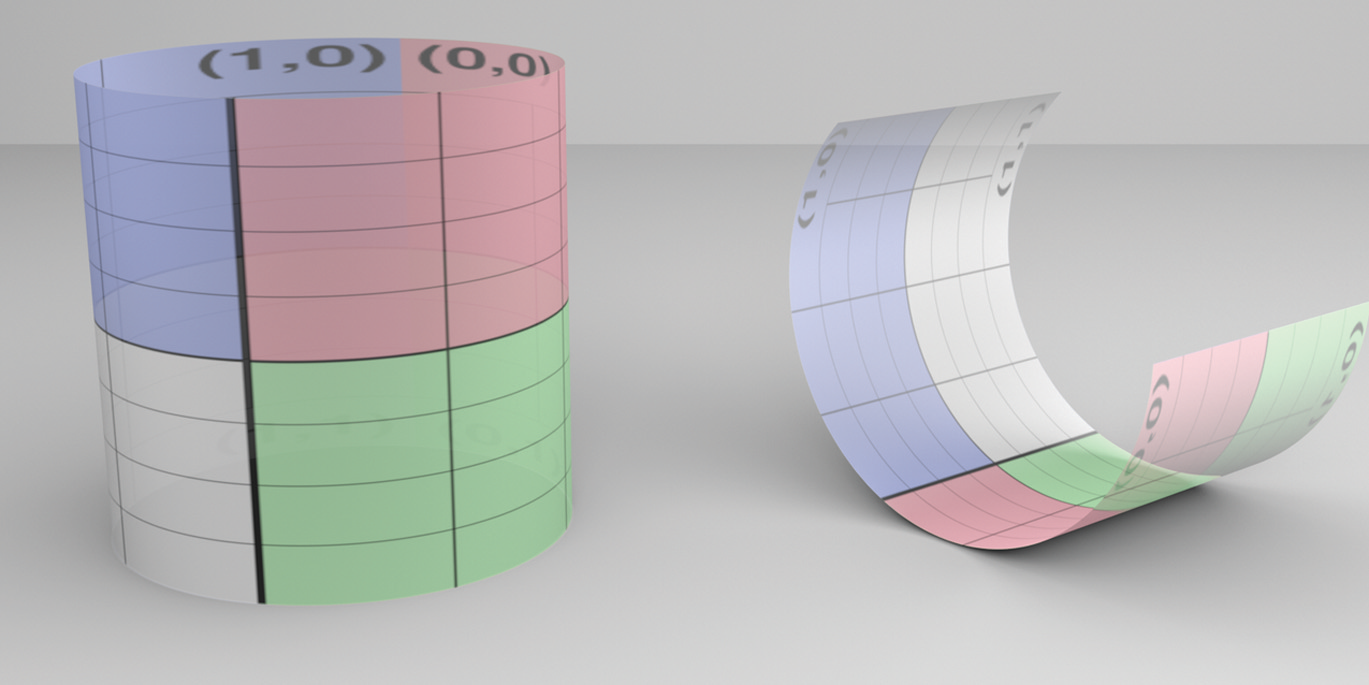
\includegraphics[width=\linewidth]{chap03/twocylinders.png}
    \caption{两个圆柱体。左边是完整圆柱体,右边是部分圆柱体。}
    \label{fig:3.7}
\end{figure}

\begin{lstlisting}
`\initcode{Cylinder Public Methods}{=}`
`\refvar{Cylinder}{}`(const `\refvar{Transform}{}` *ObjectToWorld, const `\refvar{Transform}{}` *WorldToObject,
         bool reverseOrientation, `\refvar{Float}{}` radius, `\refvar{Float}{}` zMin, `\refvar{Float}{}` zMax,
         `\refvar{Float}{}` phiMax)
    : `\refvar{Shape}{}`(ObjectToWorld, WorldToObject, reverseOrientation),
      `\refvar[Cylinder::radius]{radius}{}`(radius), `\refvar[Cylinder::zMin]{zMin}{}`(std::min(zMin, zMax)),
      `\refvar[Cylinder::zMax]{zMax}{}`(std::max(zMin, zMax)),
      `\refvar[Cylinder::phiMax]{phiMax}{}`(`\refvar{Radians}{}`(`\refvar{Clamp}{}`(phiMax, 0, 360))) { }
\end{lstlisting}
\begin{lstlisting}
`\initcode{Cylinder Private Data}{=}`
const `\refvar{Float}{}` `\initvar[Cylinder::radius]{radius}{}`, `\initvar[Cylinder::zMin]{zMin}{}`, `\initvar[Cylinder::zMax]{zMax}{}`, `\initvar[Cylinder::phiMax]{phiMax}{}`;
\end{lstlisting}

\subsection{边界}\label{sub:边界3}
像球那样,圆柱体边界方法用$z$的范围计算保守边界框但不考虑最大的$\varphi$。
\begin{lstlisting}
`\initcode{Cylinder Method Definitions}{=}\initnext{CylinderMethodDefinitions}`
`\refvar{Bounds3f}{}` `\refvar{Cylinder}{}`::`\initvar[Cylinder::ObjectBound]{\refvar{ObjectBound}{}}{}`() const {
    return `\refvar{Bounds3f}{}`(`\refvar{Point3f}{}`(-`\refvar[Cylinder::radius]{radius}{}`, -`\refvar[Cylinder::radius]{radius}{}`, `\refvar[Cylinder::zMin]{zMin}{}`),
                    `\refvar{Point3f}{}`( `\refvar[Cylinder::radius]{radius}{}`,  `\refvar[Cylinder::radius]{radius}{}`, `\refvar[Cylinder::zMax]{zMax}{}`));
}
\end{lstlisting}

\subsection{相交测试}\label{sub:相交测试3}
光线-圆柱体相交公式可以通过把射线方程代入圆柱体的隐式方程得到,和球体的情况一样。
以$z$轴为中心$r$为半径的无限长圆柱体的隐式方程为
\begin{align*}
    x^2+y^2-r^2=0\, .
\end{align*}
代入射线方程\refeq{2.3},我们有
\begin{align*}
    (o_x+td_x)^2+(o_y+td_y)^2=r^2\, .
\end{align*}
我们将其展开并求二次式方程$at^2+bt+c=0$的系数得
\begin{align*}
    a & =d_x^2+d_y^2\, ,      \\
    b & =2(d_xo_x+d_yo_y)\, , \\
    c & =o_x^2+o_y^2-r^2\, .
\end{align*}
\begin{lstlisting}
`\initcode{Compute quadratic cylinder coefficients}{=}`
`\refcode{Initialize EFloat ray coordinate values}{}`
`\refvar{EFloat}{}` a = dx * dx + dy * dy;
`\refvar{EFloat}{}` b = 2 * (dx * ox + dy * oy);
`\refvar{EFloat}{}` c = ox * ox + oy * oy - `\refvar{EFloat}{}`(`\refvar[Cylinder::radius]{radius}{}`) * `\refvar{EFloat}{}`(`\refvar[Cylinder::radius]{radius}{}`);
\end{lstlisting}

所有二次曲面形状求解二次方程的过程都一样,
所以下面会复用来自\refvar{Sphere}{}
相交方法的一些代码片。
\begin{lstlisting}
`\refcode{Cylinder Method Definitions}{+=}\lastnext{CylinderMethodDefinitions}`
bool `\refvar{Cylinder}{}`::`\initvar[Cylinder::Intersect]{\refvar[Shape::Intersect]{Intersect}{}}{}`(const `\refvar{Ray}{}` &r, `\refvar{EFloat}{}` *tHit,
        `\refvar{SurfaceInteraction}{}` *isect, bool testAlphaTexture) const {
    `\refvar{Float}{}` phi;
    `\refvar{Point3f}{}` pHit;
    `\refcode{Transform Ray to object space}{}`
    `\refcode{Compute quadratic cylinder coefficients}{}`
    `\refcode{Solve quadratic equation for t values}{}`
    `\refcode{Compute cylinder hit point and $\varphi$}{}`
    `\refcode{Test cylinder intersection against clipping parameters}{}`
    `\refcode{Find parametric representation of cylinder hit}{}`
    `\refcode{Compute error bounds for cylinder intersection}{}`
    `\refcode{Initialize SurfaceInteraction from parametric information}{}`
    `\refcode{Update tHit for quadric intersection}{}`
    return true;
}
\end{lstlisting}

像球体那样,这里的实现改进了计算的交点
以降低在计算射线方程中累积舍入误差的影响;见\refsub{定界交点误差}。
于是我们由圆柱体的参数化描述从$x$和$y$反解出$\varphi$;
最后所得结果与球体相同。
\begin{lstlisting}
`\initcode{Compute cylinder hit point and $\varphi$}{=}`
pHit = ray((`\refvar{Float}{}`)tShapeHit);
`\refcode{Refine cylinder intersection point}{}`
phi = std::atan2(pHit.y, pHit.x);
if (phi < 0) phi += 2 * `\refvar{Pi}{}`;
\end{lstlisting}

相交方法下一部分保证命中点在指定$z$范围内且能接受角度$\varphi$。
否则它就拒绝该命中点,并在之前还没尝试的前提下检查$t_1$——这和
\refvar{Sphere::Intersect}{()}
中的条件逻辑很像。
\begin{lstlisting}
`\initcode{Test cylinder intersection against clipping parameters}{=}`
if (pHit.z < `\refvar[Cylinder::zMin]{zMin}{}` || pHit.z > `\refvar[Cylinder::zMax]{zMax}{}` || phi > `\refvar[Cylinder::phiMax]{phiMax}{}`) {
    if (tShapeHit == t1) return false;
    tShapeHit = t1;
    if (t1.`\refvar{UpperBound}{}`() > ray.`\refvar{tMax}{}`) return false;
    `\refcode{Compute cylinder hit point and $\varphi$}{}`
    if (pHit.z < `\refvar[Cylinder::zMin]{zMin}{}` || pHit.z > `\refvar[Cylinder::zMax]{zMax}{}` || phi > `\refvar[Cylinder::phiMax]{phiMax}{}`)
        return false;
}
\end{lstlisting}

再次将$\varphi$缩放到0到1计算$u$值。
直接反解圆柱体参数方程的$z$值求得$v$参数坐标。
\begin{lstlisting}
`\initcode{Find parametric representation of cylinder hit}{=}`
`\refvar{Float}{}` u = phi / `\refvar[Cylinder::phiMax]{phiMax}{}`;
`\refvar{Float}{}` v = (pHit.z - `\refvar[Cylinder::zMin]{zMin}{}`) / (`\refvar[Cylinder::zMax]{zMax}{}` - `\refvar[Cylinder::zMin]{zMin}{}`);
`\refcode{Compute cylinder $\partial$p/$\partial$u and $\partial$p/$\partial$v}{}`
`\refcode{Compute cylinder $\partial$n/$\partial$u and $\partial$n/$\partial$v}{}`
\end{lstlisting}

圆柱体的偏导数很容易推导:
\begin{align*}
    \frac{\partial\bm p}{\partial u} & =(-\varphi_{\max}y,\varphi_{\max}x,0)\, , \\
    \frac{\partial\bm p}{\partial v} & =(0,0,z_{\max}-z_{\min})\, .
\end{align*}
\begin{lstlisting}
`\initcode{Compute cylinder $\partial$p/$\partial$u and $\partial$p/$\partial$v}{=}`
`\refvar{Vector3f}{}` dpdu(-`\refvar[Cylinder::phiMax]{phiMax}{}` * pHit.y, `\refvar[Cylinder::phiMax]{phiMax}{}` * pHit.x, 0);
`\refvar{Vector3f}{}` dpdv(0, 0, `\refvar[Cylinder::zMax]{zMax}{}` - `\refvar[Cylinder::zMin]{zMin}{}`);
\end{lstlisting}

我们又用Weingarten方程计算圆柱法线的参数化偏导数。
相关偏导数为:
\begin{align*}
    \frac{\partial^2\bm p}{\partial u^2}         & =-\varphi_{\max}^2(x,y,0)\, , \\
    \frac{\partial^2\bm p}{\partial u\partial v} & =(0,0,0)\, ,                  \\
    \frac{\partial^2\bm p}{\partial v^2}         & =(0,0,0)\, .
\end{align*}
\begin{lstlisting}
`\initcode{Compute cylinder $\partial$n/$\partial$u and $\partial$n/$\partial$v}{=}`
`\refvar{Vector3f}{}` d2Pduu = -`\refvar[Cylinder::phiMax]{phiMax}{}` * `\refvar[Cylinder::phiMax]{phiMax}{}` * `\refvar{Vector3f}{}`(pHit.x, pHit.y, 0);
`\refvar{Vector3f}{}` d2Pduv(0, 0, 0), d2Pdvv(0, 0, 0);
`\refcode{Compute coefficients for fundamental forms}{}`
`\refcode{Compute $\partial$n/$\partial$u and $\partial$n/$\partial$v from fundamental form coefficients}{}`
\end{lstlisting}

\subsection{表面积}\label{sub:表面积3}
圆柱体就是卷起来的矩形。如果你展开矩形,
其高是$z_{\max}-z_{\min}$,宽是$r\varphi_{\max}$:
\begin{lstlisting}
`\refcode{Cylinder Method Definitions}{+=}\lastnext{CylinderMethodDefinitions}`
`\refvar{Float}{}` `\refvar{Cylinder}{}`::`\initvar[Cylinder::Area]{\refvar[Shape::Area]{Area}{}}{}`() const {
    return (`\refvar[Cylinder::zMax]{zMax}{}` - `\refvar[Cylinder::zMin]{zMin}{}`) * `\refvar[Cylinder::radius]{radius}{}` * `\refvar[Cylinder::phiMax]{phiMax}{}`;
}
\end{lstlisting}

\section{圆盘}\label{sec:圆盘}

\keyindex{圆盘}{disk}{}是一种有趣的二次曲面,
因为它有特别简单的相交例程避免求解二次方程。

\section{其他二次曲面}\label{sec:其他二次曲面}

\section{三角形网格}\label{sec:三角形网格}
\keyindex{三角形}{triangle}{}是计算机图形学最常用的形状;
复杂场景会用上百万三角形建模以实现出色细节
(\reffig{3.11}展示了四百多万三角形的复杂三角网格图像)。
\begin{figure}[htb]
    \centering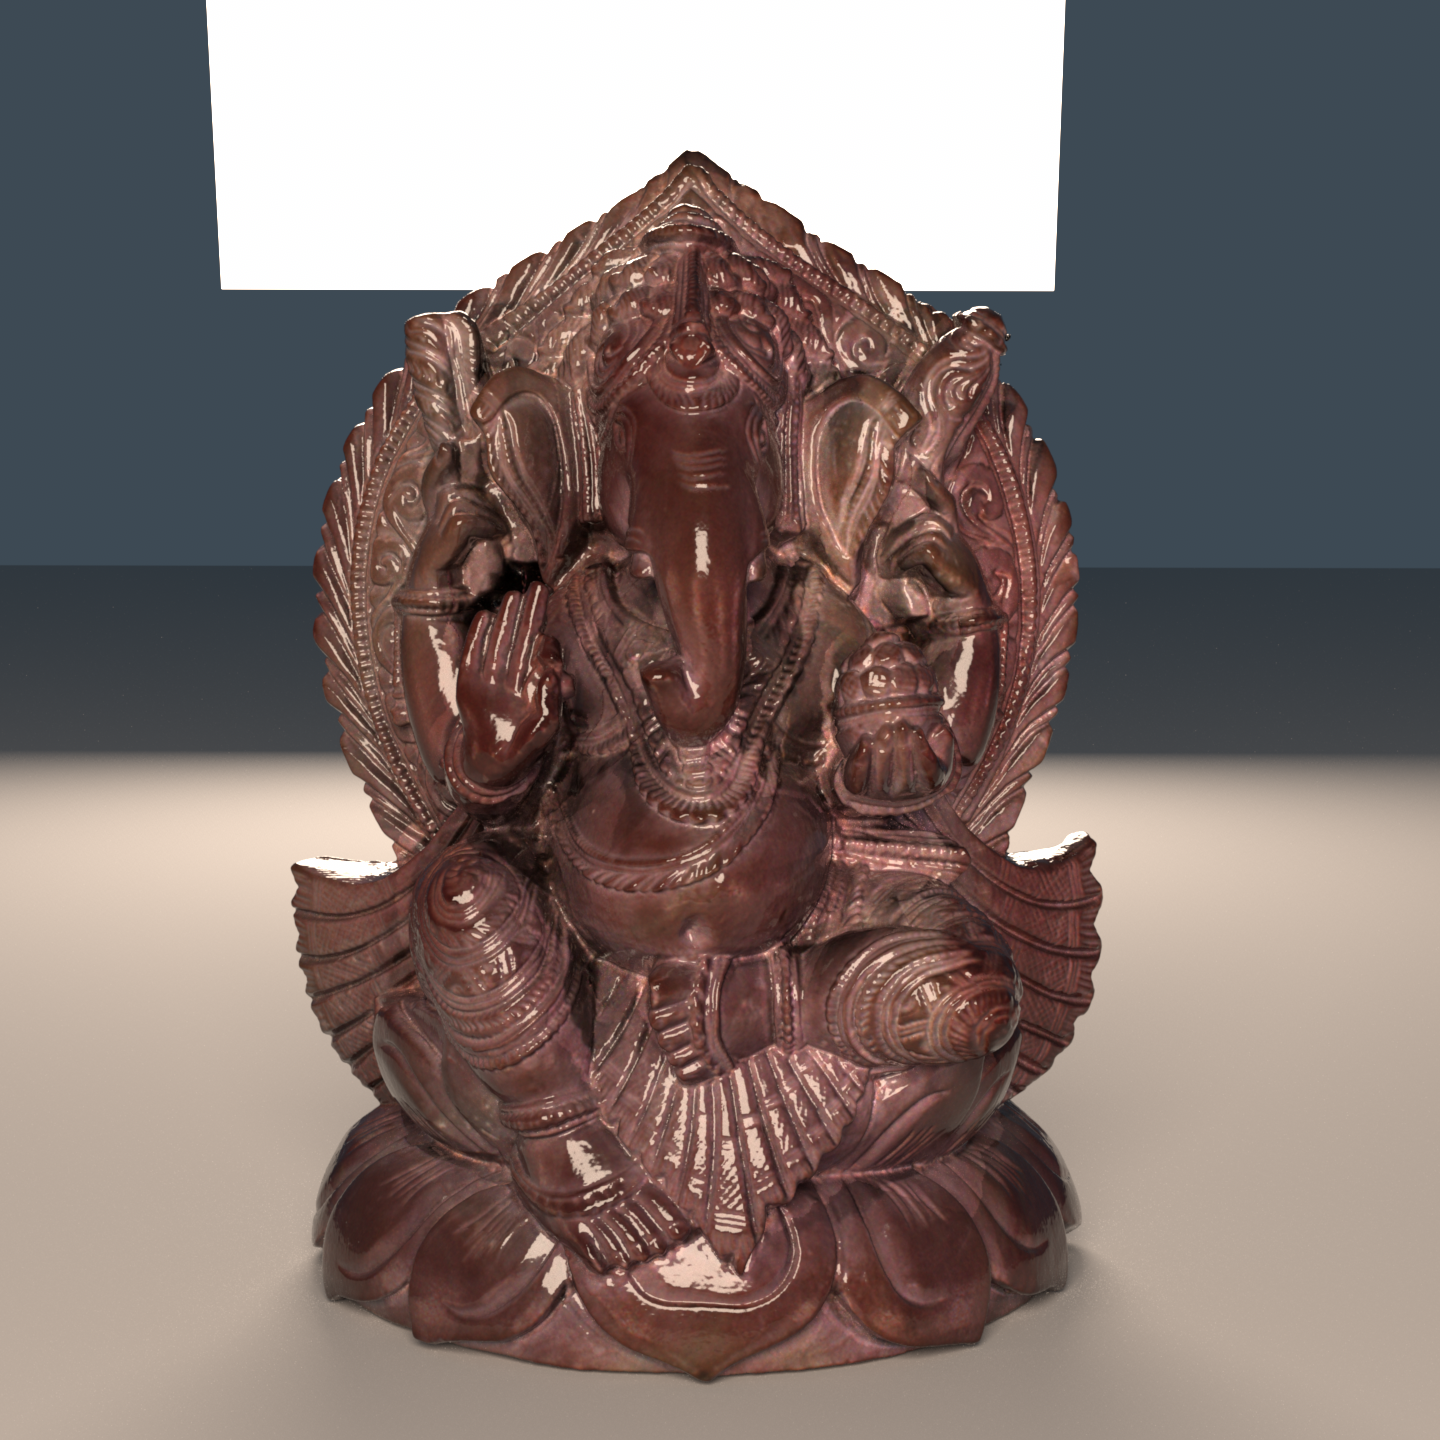
\includegraphics[width=\linewidth]{chap03/ganesha.png}
    \caption{象头神模型。该三角网格含有四百多万个独立三角形。
        它是使用结构光确定物体形状的3D扫描器用真实雕塑创建的。}
    \label{fig:3.11}
\end{figure}

尽管自然的表示是用{\ttfamily Triangle}形状实现,
每个三角形都存储其三个\keyindex{顶点}{vertex}{}的位置,
但内存更高效的表示是用顶点位置数组分开存储整个\keyindex{三角网格}{triangle mesh}{mesh网格},
每个独立三角形只存储其三个顶点对该数组的三个偏移量。

为了理解该做法,考虑著名的\keyindex{欧拉-庞加莱公式}{Euler-Poincaré formula}{},
它将闭合离散\keyindex{网格}{mesh}{}的顶点数$V$、\keyindex{边}{edge}{}数$E$和\keyindex{面}{face}{}数$F$联系起来:
\begin{align*}
    V-E+F=2(1-g)\, ,
\end{align*}
其中$g\in\mathbb{N}$是网格的\keyindex{亏格}{genus}{}。
亏格通常是很小的数且能解释为网格的“手柄”数量(类似于茶杯把手)。
在三角网格上,边数和面数\sidenote{译者注:原文错写为顶点数,已修改。}还由恒等式联系
\begin{align*}
    E=\frac{3}{2}F\, .
\end{align*}
这可以看作把每条边分成两部分与两个相邻三角形关联。
有$3F$条这样的半边,所有同位的边对构成$E$条网格边。
对于巨大的闭合三角网格,亏格的整体影响通常可以忽略,
我们可以结合之前两个方程(以及$g=0$)得到
\begin{align*}
    F\approx2V\, .
\end{align*}
换句话说,面数大约是顶点数的两倍。
既然每个面引用三个顶点,每个顶点(平均)总共被引用六次。
因此当共享顶点时,每个三角形所需的总分摊存储为
偏移量的12字节内存(三个4字节32位整数偏移量)加上一个顶点存储的一半——6字节,
这里假设每个顶点用三个4字节浮点存储——每个三角形一共18字节。
这比每个三角形直接用36字节存储三个位置好得多。
当网格中有每个顶点的曲面法线或纹理坐标时,相对的存储节约会更好。

pbrt使用结构体\refvar{TriangleMesh}{}保存关于三角网格的共享信息。
\begin{lstlisting}
`\initcode{Triangle Declarations}{=}\initnext{TriangleDeclarations}`
struct `\initvar{TriangleMesh}{}` {
    `\refcode{TriangleMesh Public Methods}{}`
    `\refcode{TriangleMesh Data}{}`
};
\end{lstlisting}
\begin{lstlisting}
`\initcode{TriangleMesh Public Methods}{=}`
`\refvar{TriangleMesh}{}`(const `\refvar{Transform}{}` &ObjectToWorld, int nTriangles, const int *vertexIndices,
    int nVertices, const `\refvar{Point3f}{}` *P, const `\refvar{Vector3f}{}` *S, const `\refvar{Normal3f}{}` *N,
    const `\refvar{Point2f}{}` *uv, const std::shared_ptr<`\refvar{Texture}{}`<`\refvar{Float}{}`>> &alphaMask);
\end{lstlisting}

\refvar{TriangleMesh}{}构造函数的参数如下:
\begin{itemize}
    \item {\ttfamily ObjectToWorld}:网格的物体到世界的变换。
    \item {\ttfamily nTriangles}:网格中三角形总数。
    \item {\ttfamily vertexIndices}:指向顶点索引数组的指针。对于第{\ttfamily i}个三角形,其三个顶点位置为
          {\ttfamily P[vertexIndices[3*i]]}、{\ttfamily P[vertexIndices[3*i+1]]}和{\ttfamily P[vertexIndices[3*i+2]]}。
    \item {\ttfamily nVertices}:网格中顶点总数。
    \item {\ttfamily P}:{\ttfamily nVertices}个顶点位置的数组。
    \item {\ttfamily S}:可选切向量数组,网格中每个顶点都有一个。它们用于计算着色切线。
    \item {\ttfamily N}:可选法向量数组,网格中每个顶点都有一个。如果有,则它们在三角形面之间插值以计算着色法线。
    \item {\ttfamily UV}:可选参数值$(u,v)$数组,每个顶点一个。
    \item {\ttfamily alphaMask}:可选的\keyindex{$\alpha$掩模}{alpha mask}{}纹理,可用于截去部分三角形面。
\end{itemize}

pbrt中三角形在形状里有双重角色:不仅场景描述文件经常直接指定它们,
其他形状也常把自己细分为三角网格。
例如,细分曲面最终创建一个三角网格来近似光滑有限曲面。
再对这些三角形执行光线相交,而不是直接对细分曲面这样做(\refsub{细分})。

由于这第二种角色,创建三角网格的代码能指定三角形的参数化很重要。
如果三角形是通过求取参数化曲面在三个特定坐标值$(u,v)$处的位置来创建的,
这些$(u,v)$值应该被插值以计算三角形内光线交点处的$(u,v)$值。
显式指定$(u,v)$值对纹理贴图也很有用,创建三角网格的外部程序
可能想给网格赋值$(u,v)$坐标,这样纹理贴图以期望的方式把颜色赋值给网格曲面。

\refvar{TriangleMesh}{}构造函数赋值相关信息并存于成员变量中。
特别地,它自己复制{\ttfamily vertexIndices、P、N、S}和{\ttfamily UV},
允许调用者保留对传入数据的所有权。
\begin{lstlisting}
`\initcode{Triangle Method Definitions}{=}\initnext{TriangleMethodDefinitions}`
`\refvar{TriangleMesh}{}`::`\refvar{TriangleMesh}{}`(const `\refvar{Transform}{}` &ObjectToWorld,
        int nTriangles, const int *vertexIndices, int nVertices,
        const `\refvar{Point3f}{}` *P, const `\refvar{Vector3f}{}` *S, const `\refvar{Normal3f}{}` *N,
        const `\refvar{Point3f}{}` *UV,
        const std::shared_ptr<`\refvar{Texture}{}`<`\refvar{Float}{}`>> &alphaMask)
    : `\refvar{nTriangles}{}`(nTriangles), `\refvar{nVertices}{}`(nVertices), 
      `\refvar{vertexIndices}{}`(vertexIndices, vertexIndices + 3 * nTriangles),
      `\refvar{alphaMask}{}`(alphaMask) {
    `\refcode{Transform mesh vertices to world space}{}`
    `\refcode{Copy UV, N, and S vertex data, if present}{}`
}
\end{lstlisting}
\begin{lstlisting}
    `\initcode{TriangleMesh Data}{=}`
    const int `\initvar{nTriangles}{}`, `\initvar{nVertices}{}`;
    std::vector<int> `\initvar{vertexIndices}{}`;
    std::unique_ptr<`\refvar{Point3f}{}`[]> `\initvar[TriangleMesh::p]{p}{}`;
    std::unique_ptr<`\refvar{Normal3f}{}`[]> `\initvar[TriangleMesh::n]{n}{}`;
    std::unique_ptr<`\refvar{Vector3f}{}`[]> `\initvar[TriangleMesh::s]{s}{}`;
    std::unique_ptr<`\refvar{Point2f}{}`[]> `\initvar[TriangleMesh::uv]{uv}{}`;
    std::shared_ptr<`\refvar{Texture}{}`<`\refvar{Float}{}`>> `\initvar{alphaMask}{}`;
\end{lstlisting}

不像其他形状那样把形状描述留在物体空间内然后
将入射光线从世界空间变换到物体空间,
三角网格将形状变换到世界空间,
因此节约了把入射光线变换到物体空间的工作和
把相交处的几何表示变换出世界空间的工作。
这是个好主意,因为该操作可在启动后执行,
避免渲染中多次变换光线。
尽管也能对二次曲面使用该方法,但会更复杂(见本章末习题7了解更多信息)。
\begin{lstlisting}
`\initcode{Transform mesh vertices to world space}{=}`
`\refvar[TriangleMesh::p]{p}{}`.reset(new `\refvar{Point3f}{}`[`\refvar{nVertices}{}`]);
for (int i = 0; i < `\refvar{nVertices}{}`; ++i)
    `\refvar[TriangleMesh::p]{p}{}`[i] = ObjectToWorld(P[i]);
\end{lstlisting}

代码片\refcode{Copy UV, N, and S vertex data, if present}{}只是
分配合适数量的空间并复制合适的值。
如果有法线和切向量,则也变换到世界空间。
\begin{lstlisting}
`\initcode{Copy UV, N, and S vertex data, if present}{=}`
if (UV) {
    `\refvar[TriangleMesh::uv]{uv}{}`.reset(new `\refvar{Point2f}{}`[`\refvar{nVertices}{}`]);
    memcpy(`\refvar[TriangleMesh::uv]{uv}{}`.get(), UV, `\refvar{nVertices}{}` * sizeof(`\refvar{Point2f}{}`));
}
if (N) {
    `\refvar[TriangleMesh::n]{n}{}`.reset(new `\refvar{Normal3f}{}`[`\refvar{nVertices}{}`]);
    for (int i = 0; i < `\refvar{nVertices}{}`; ++i)
        `\refvar[TriangleMesh::n]{n}{}`[i] = ObjectToWorld(N[i]);
}
if (S) {
    `\refvar[TriangleMesh::s]{s}{}`.reset(new `\refvar{Vector3f}{}`[`\refvar{nVertices}{}`]);
    for (int i = 0; i < `\refvar{nVertices}{}`; ++i)
        `\refvar[TriangleMesh::s]{s}{}`[i] = ObjectToWorld(S[i]);
}
\end{lstlisting}

\subsection{三角形}\label{sub:三角形}
类\refvar{Triangle}{}实际上实现了\refvar{Shape}{}接口。它表示单个三角形。
\begin{lstlisting}
`\refcode{Triangle Declarations}{+=}\lastcode{TriangleDeclarations}`
class `\initvar{Triangle}{}` : public `\refvar{Shape}{}` {
public:
    `\refcode{Triangle Public Methods}{}`
private:
    `\refcode{Triangle Private Methods}{}`
    `\refcode{Triangle Private Data}{}`
};
\end{lstlisting}

\refvar{Triangle}{}不存储太多数据——只有一个指向其来处的父\refvar{TriangleMesh}{}指针
和一个指向网格中其三个顶点索引的指针。
\begin{lstlisting}
`\initcode{Triangle Public Methods}{=}`
`\refvar{Triangle}{}`(const `\refvar{Transform}{}` *ObjectToWorld, const `\refvar{Transform}{}` *WorldToObject,
         bool reverseOrientation,
         const std::shared_ptr<`\refvar{TriangleMesh}{}`> &mesh, int triNumber)
    : `\refvar{Shape}{}`(ObjectToWorld, WorldToObject, reverseOrientation),
      `\refvar{mesh}{}`(mesh) {
    `\refvar[Triangle::v]{v}{}` = &mesh->`\refvar{vertexIndices}{}`[3 * triNumber];
}
\end{lstlisting}

注意该实现存储了指向第一个顶点\emph{索引}的指针,
而非存储三个指向顶点自己的指针。
这以另一级别的间接性为代价减少了每个\refvar{Triangle}{}所需的存储量。
\begin{lstlisting}
`\initcode{Triangle Private Data}{=}`
std::shared_ptr<`\refvar{TriangleMesh}{}`> `\initvar{mesh}{}`;
const int *`\initvar[Triangle::v]{v}{}`;
\end{lstlisting}

因为pbrt中大量的其他形状表示会把自己转化为三角网格,
实用函数
\refvar{CreateTriangleMesh}{()}仔细创建
底层\refvar{TriangleMesh}{}以及网格中每个三角形的\refvar{Triangle}{}。
它返回三角形状的向量。
\begin{lstlisting}
`\refcode{Triangle Method Definitions}{+=}\lastnext{TriangleMethodDefinitions}`
std::vector<std::shared_ptr<`\refvar{Shape}{}`>> `\initvar{CreateTriangleMesh}{}`(
        const `\refvar{Transform}{}` *ObjectToWorld, const `\refvar{Transform}{}` *WorldToObject,
        bool reverseOrientation, int nTriangles,
        const int *vertexIndices, int nVertices, const `\refvar{Point3f}{}` *p,
        const `\refvar{Vector3f}{}` *s, const `\refvar{Normal3f}{}` *n, const `\refvar{Point2f}{}` *uv,
        const std::shared_ptr<`\refvar{Texture}{}`<`\refvar{Float}{}`>> &alphaMask) {
    std::shared_ptr<`\refvar{TriangleMesh}{}`> mesh = std::make_shared<`\refvar{TriangleMesh}{}`>(
        *ObjectToWorld, nTriangles, vertexIndices, nVertices, p, s, n, uv,
        alphaMask);
    std::vector<std::shared_ptr<`\refvar{Shape}{}`>> tris;
    for (int i = 0; i < nTriangles; ++i)
        tris.push_back(std::make_shared<`\refvar{Triangle}{}`>(ObjectToWorld,
            WorldToObject, reverseOrientation, mesh, i));
    return tris;
}
\end{lstlisting}

三角形的物体空间边界很容易通过计算包围其三个顶点的边界框求得。
因为顶点位置\refvar[TriangleMesh::p]{p}{}在构造函数中被变换到世界空间,
这里的实现要在计算其边界前把它们变换回物体空间。
\begin{lstlisting}
`\refcode{Triangle Method Definitions}{+=}\lastnext{TriangleMethodDefinitions}`
`\refvar{Bounds3f}{}` `\refvar{Triangle}{}`::`\initvar[Triangle::ObjectBound]{\refvar{ObjectBound}{}}{}`() const {
    `\refcode{Get triangle vertices in p0, p1, and p2}{}`
    return `\refvar[Union1]{Union}{}`(`\refvar{Bounds3f}{}`((*`\refvar{WorldToObject}{}`)(p0), (*`\refvar{WorldToObject}{}`)(p1)),
                 (*`\refvar{WorldToObject}{}`)(p2));
}
\end{lstlisting}
\begin{lstlisting}
`\initcode{Get triangle vertices in p0, p1, and p2}{=}`
const `\refvar{Point3f}{}` &p0 = `\refvar{mesh}{}`->`\refvar[TriangleMesh::p]{p}{}`[`\refvar[Triangle::v]{v}{}`[0]];
const `\refvar{Point3f}{}` &p1 = `\refvar{mesh}{}`->`\refvar[TriangleMesh::p]{p}{}`[`\refvar[Triangle::v]{v}{}`[1]];
const `\refvar{Point3f}{}` &p2 = `\refvar{mesh}{}`->`\refvar[TriangleMesh::p]{p}{}`[`\refvar[Triangle::v]{v}{}`[2]];
\end{lstlisting}

比起变换其物体空间边界框到世界空间,
\refvar{Triangle}{}形状是能计算更好的世界空间边界的形状之一。
其世界空间边界可以直接从世界空间顶点算得。
\begin{lstlisting}
`\refcode{Triangle Method Definitions}{+=}\lastnext{TriangleMethodDefinitions}`
`\refvar{Bounds3f}{}` `\refvar{Triangle}{}`::`\initvar[Triangle::WorldBound]{\refvar[Shape::WorldBound]{WorldBound}{}}{}`() const {
    `\refcode{Get triangle vertices in p0, p1, and p2}{}`
    return `\refvar[Union1]{Union}{}`(`\refvar{Bounds3f}{}`(p0, p1), p2); 
}
\end{lstlisting}

\subsection{三角形相交}\label{sub:三角形相交}
三角形状方法\refvar[Triangle::Intersect]{Intersect}{()}的结构
遵循之前的相交测试方法:应用几何测试以确定是否相交,
如果有,则计算更多关于相交的信息,并在给定的
\refvar{SurfaceInteraction}{}中返回。
\begin{lstlisting}
`\refcode{Triangle Method Definitions}{+=}\lastnext{TriangleMethodDefinitions}`
bool `\initvar{Triangle::Intersect}{}`(const `\refvar{Ray}{}` &ray, `\refvar{Float}{}` *tHit,
        `\refvar{SurfaceInteraction}{}` *isect, bool testAlphaTexture) const {
    `\refcode{Get triangle vertices in p0, p1, and p2}{}`
    `\refcode{Perform ray–triangle intersection test}{}`
    `\refcode{Compute triangle partial derivatives}{}`
    `\refcode{Compute error bounds for triangle intersection}{}`
    `\refcode{Interpolate (u,v) parametric coordinates and hit point}{}`
    `\refcode{Test intersection against alpha texture, if present}{}`
    `\refcode{Fill in SurfaceInteraction from triangle hit}{}`
    *tHit = t;
    return true;
}
\end{lstlisting}

pbrt的光线-三角形相交测试基于首先计算仿射变换
使得射线在变换后的坐标系里端点被变换为$(0,0,0)$且其方向沿$+z$轴。
在执行相机测试之前三角形顶点也变换到该坐标系。
下面我们将看到应用该坐标系变换会简化相交测试逻辑,
例如任何交点的$x$和$y$坐标必须为零。
之后在\refsub{稳定的三角形相交},我们会看到该变换让
拥有\keyindex{水密的}{watertight}{}光线-三角形相交算法成为可能,
这样刚好命中三角形边缘的棘手光线等的相交就永远不会被错误地报告为未命中了。
\begin{lstlisting}
`\initcode{Perform ray–triangle intersection test}{=}`
`\refcode{Transform triangle vertices to ray coordinate space}{}`
`\refcode{Compute edge function coefficients e0, e1, and e2}{}`
`\refcode{Fall back to double-precision test at triangle edges}{}`
`\refcode{Perform triangle edge and determinant tests}{}`
`\refcode{Compute scaled hit distance to triangle and test against ray t range}{}`
`\refcode{Compute barycentric coordinates and t value for triangle intersection}{}`
`\refcode{Ensure that computed triangle t is conservatively greater than zero}{}`
\end{lstlisting}

计算从世界空间到光线-三角形相交坐标空间的变换有三步:
平移$\bm T$、坐标\keyindex{置换}{permutation}{}$\bm P$和\keyindex{错切}{shear}{}$\bm S$。
下列实现没有为它们每个都计算显式的变换矩阵
再计算合成变换矩阵$\bm M=\bm S\bm P\bm T$来把顶点变换到坐标空间,
而是直接施加每步的变换,这最终是更高效的方法。
\begin{lstlisting}
`\initcode{Transform triangle vertices to ray coordinate space}{=}`
`\refcode{Translate vertices based on ray origin}{}`
`\refcode{Permute components of triangle vertices and ray direction}{}`
`\refcode{Apply shear transformation to translated vertex positions}{}`
\end{lstlisting}

将射线端点放置在坐标系的原点的平移是:
\begin{align*}
    \bm T=\left[\begin{array}{cccc}
            1 & 0 & 0 & -o_x \\
            0 & 1 & 0 & -o_y \\
            0 & 0 & 1 & -o_z \\
            0 & 0 & 0 & 1
        \end{array}\right]\, .
\end{align*}
该变换不需要显式施加到射线端点,但我们会将其施加于三角形三个顶点。
\begin{lstlisting}
`\initcode{Translate vertices based on ray origin}{=}`
`\refvar{Point3f}{}` p0t = p0 - `\refvar{Vector3f}{}`(ray.o);
`\refvar{Point3f}{}` p1t = p1 - `\refvar{Vector3f}{}`(ray.o);
`\refvar{Point3f}{}` p2t = p2 - `\refvar{Vector3f}{}`(ray.o);
\end{lstlisting}

接下来,置换空间三个维度使得$z$维的射线方向绝对值最大。
$x$和$y$维任意分配给另外两维。
例如,这步保证如果原始射线的$z$方向为零,
则非零幅度的维度映射到$+z$。

例如,如果光线方向在$x$有最大幅值,则置换为:
\begin{align*}
    \bm P=\left[\begin{array}{cccc}
            0 & 1 & 0 & 0 \\
            0 & 0 & 1 & 0 \\
            1 & 0 & 0 & 0 \\
            0 & 0 & 0 & 1
        \end{array}\right]\, .
\end{align*}

像之前那样,直接置换射线方向维度和平移后的三角形顶点最简单。
\begin{lstlisting}
`\initcode{Permute components of triangle vertices and ray direction}{=}`
int kz = `\refvar{MaxDimension}{}`(`\refvar[Vector3::Abs]{Abs}{}`(ray.d));
int kx = kz + 1; if (kx == 3) kx = 0;
int ky = kx + 1; if (ky == 3) ky = 0;
`\refvar{Vector3f}{}` d = `\refvar[Vector3::Permute]{Permute}{}`(ray.d, kx, ky, kz);
p0t = `\refvar[Point3::Permute]{Permute}{}`(p0t, kx, ky, kz);
p1t = `\refvar[Point3::Permute]{Permute}{}`(p1t, kx, ky, kz);
p2t = `\refvar[Point3::Permute]{Permute}{}`(p2t, kx, ky, kz);
\end{lstlisting}

最后,错切变换将射线方向与$+z$轴对齐:
\begin{align*}
    \bm S=\left[\begin{array}{rrrr}
            1 & 0 & \displaystyle-\frac{d_x}{d_z} & 0 \\
            0 & 1 & \displaystyle-\frac{d_y}{d_z} & 0 \\
            0 & 0 & \displaystyle\frac{1}{d_z}    & 0 \\
            0 & 0 & 0                             & 1
        \end{array}\right]\, .
\end{align*}
为了理解该变换如何工作,可考虑它对射线方向向量$[d_x\ d_y\ d_z\ 0]^{\mathrm{T}}$的操作。

现在,只有$x$和$y$维被错切;我们可以等到只有当光线确实与三角形相交时再错切$z$维。
\begin{lstlisting}
`\initcode{Apply shear transformation to translated vertex positions}{=}`
`\refvar{Float}{}` Sx = -d.x / d.z;
`\refvar{Float}{}` Sy = -d.y / d.z;
`\refvar{Float}{}` Sz = 1.f / d.z;
p0t.x += Sx * p0t.z;
p0t.y += Sy * p0t.z;
p1t.x += Sx * p1t.z;
p1t.y += Sy * p1t.z;
p2t.x += Sx * p2t.z;
p2t.y += Sy * p2t.z;
\end{lstlisting}

注意坐标置换和错切系数的计算只取决于给定的光线;
它们和三角形无关。在高性能光线追踪器里,
我们可能想一次性计算这些值并保存在类\refvar{Ray}{}里,
而不是为与光线相交的每个三角形重新计算它们。

三角形顶点变换到该坐标系后,我们现在的任务是求从原点出发
并沿$+z$的光线是否与变换后的三角形相交。
因为构造坐标系的方式,该问题等价于2D问题即
确定$x,y$坐标$(0,0)$是否在三角形的$xy$投影内(\reffig{3.12})。
\begin{figure}[htbp]
    \centering%LaTeX with PSTricks extensions
%%Creator: Inkscape 1.0.1 (3bc2e813f5, 2020-09-07)
%%Please note this file requires PSTricks extensions
\psset{xunit=.5pt,yunit=.5pt,runit=.5pt}
\begin{pspicture}(332.77999878,185.77000427)
{
\newrgbcolor{curcolor}{0 0 0}
\pscustom[linewidth=1,linecolor=curcolor]
{
\newpath
\moveto(221.52,1.94000427)
\lineto(329.48,49.12000427)
\lineto(270.78,181.22000427)
\closepath
}
}
{
\newrgbcolor{curcolor}{0 0 0}
\pscustom[linewidth=1,linecolor=curcolor,linestyle=dashed,dash=4]
{
\newpath
\moveto(94.86000061,84.16000366)
\lineto(281.83999634,84.16000366)
}
}
{
\newrgbcolor{curcolor}{0 0 0}
\pscustom[linewidth=1,linecolor=curcolor]
{
\newpath
\moveto(25.56999969,84.16000366)
\lineto(86.76000214,84.16000366)
}
}
{
\newrgbcolor{curcolor}{0 0 0}
\pscustom[linestyle=none,fillstyle=solid,fillcolor=curcolor]
{
\newpath
\moveto(81.85,78.66000427)
\lineto(86.11,84.16000427)
\lineto(81.85,89.67000427)
\lineto(94.86,84.16000427)
\closepath
}
}
{
\newrgbcolor{curcolor}{0.65098041 0.65098041 0.65098041}
\pscustom[linestyle=none,fillstyle=solid,fillcolor=curcolor]
{
\newpath
\moveto(83.41,79.86000427)
\lineto(93.55,84.16000427)
\lineto(86.74,84.16000427)
\closepath
}
}
{
\newrgbcolor{curcolor}{0.40000001 0.40000001 0.40000001}
\pscustom[linestyle=none,fillstyle=solid,fillcolor=curcolor]
{
\newpath
\moveto(83.41,88.46000427)
\lineto(93.55,84.16000427)
\lineto(86.74,84.16000427)
\closepath
}
}
{
\newrgbcolor{curcolor}{0 0 0}
\pscustom[linestyle=none,fillstyle=solid,fillcolor=curcolor]
{
\newpath
\moveto(28.17999983,84.19000244)
\curveto(28.17999983,86.28377436)(25.64872433,87.33195976)(24.16838347,85.8516189)
\curveto(22.68804261,84.37127804)(23.736228,81.84000254)(25.82999992,81.84000254)
\curveto(27.92377185,81.84000254)(28.97195724,84.37127804)(27.49161638,85.8516189)
\curveto(26.01127552,87.33195976)(23.48000002,86.28377436)(23.48000002,84.19000244)
\curveto(23.48000002,82.09623052)(26.01127552,81.04804512)(27.49161638,82.52838599)
\curveto(28.97195724,84.00872685)(27.92377185,86.54000235)(25.82999992,86.54000235)
\curveto(23.736228,86.54000235)(22.68804261,84.00872685)(24.16838347,82.52838599)
\curveto(25.64872433,81.04804512)(28.17999983,82.09623052)(28.17999983,84.19000244)
\closepath
}
}
{
\newrgbcolor{curcolor}{0 0 0}
\pscustom[linewidth=1,linecolor=curcolor]
{
\newpath
\moveto(28.17999983,84.19000244)
\curveto(28.17999983,86.28377436)(25.64872433,87.33195976)(24.16838347,85.8516189)
\curveto(22.68804261,84.37127804)(23.736228,81.84000254)(25.82999992,81.84000254)
\curveto(27.92377185,81.84000254)(28.97195724,84.37127804)(27.49161638,85.8516189)
\curveto(26.01127552,87.33195976)(23.48000002,86.28377436)(23.48000002,84.19000244)
\curveto(23.48000002,82.09623052)(26.01127552,81.04804512)(27.49161638,82.52838599)
\curveto(28.97195724,84.00872685)(27.92377185,86.54000235)(25.82999992,86.54000235)
\curveto(23.736228,86.54000235)(22.68804261,84.00872685)(24.16838347,82.52838599)
\curveto(25.64872433,81.04804512)(28.17999983,82.09623052)(28.17999983,84.19000244)
\closepath
}
}
{
\newrgbcolor{curcolor}{0 0 0}
\pscustom[linestyle=none,fillstyle=solid,fillcolor=curcolor]
{
\newpath
\moveto(273.01000357,182.92000437)
\curveto(273.01000357,185.01377629)(270.47872807,186.06196169)(268.99838721,184.58162082)
\curveto(267.51804634,183.10127996)(268.56623174,180.57000446)(270.66000366,180.57000446)
\curveto(272.75377558,180.57000446)(273.80196098,183.10127996)(272.32162012,184.58162082)
\curveto(270.84127926,186.06196169)(268.31000376,185.01377629)(268.31000376,182.92000437)
\curveto(268.31000376,180.82623245)(270.84127926,179.77804705)(272.32162012,181.25838791)
\curveto(273.80196098,182.73872877)(272.75377558,185.27000427)(270.66000366,185.27000427)
\curveto(268.56623174,185.27000427)(267.51804634,182.73872877)(268.99838721,181.25838791)
\curveto(270.47872807,179.77804705)(273.01000357,180.82623245)(273.01000357,182.92000437)
\closepath
}
}
{
\newrgbcolor{curcolor}{0 0 0}
\pscustom[linewidth=1,linecolor=curcolor]
{
\newpath
\moveto(273.01000357,182.92000437)
\curveto(273.01000357,185.01377629)(270.47872807,186.06196169)(268.99838721,184.58162082)
\curveto(267.51804634,183.10127996)(268.56623174,180.57000446)(270.66000366,180.57000446)
\curveto(272.75377558,180.57000446)(273.80196098,183.10127996)(272.32162012,184.58162082)
\curveto(270.84127926,186.06196169)(268.31000376,185.01377629)(268.31000376,182.92000437)
\curveto(268.31000376,180.82623245)(270.84127926,179.77804705)(272.32162012,181.25838791)
\curveto(273.80196098,182.73872877)(272.75377558,185.27000427)(270.66000366,185.27000427)
\curveto(268.56623174,185.27000427)(267.51804634,182.73872877)(268.99838721,181.25838791)
\curveto(270.47872807,179.77804705)(273.01000357,180.82623245)(273.01000357,182.92000437)
\closepath
}
}
{
\newrgbcolor{curcolor}{0 0 0}
\pscustom[linestyle=none,fillstyle=solid,fillcolor=curcolor]
{
\newpath
\moveto(223.42000723,2.8500061)
\curveto(223.42000723,4.94377803)(220.88873173,5.99196342)(219.40839087,4.51162256)
\curveto(217.92805001,3.0312817)(218.9762354,0.5000062)(221.07000732,0.5000062)
\curveto(223.16377925,0.5000062)(224.21196464,3.0312817)(222.73162378,4.51162256)
\curveto(221.25128292,5.99196342)(218.72000742,4.94377803)(218.72000742,2.8500061)
\curveto(218.72000742,0.75623418)(221.25128292,-0.29195121)(222.73162378,1.18838965)
\curveto(224.21196464,2.66873051)(223.16377925,5.20000601)(221.07000732,5.20000601)
\curveto(218.9762354,5.20000601)(217.92805001,2.66873051)(219.40839087,1.18838965)
\curveto(220.88873173,-0.29195121)(223.42000723,0.75623418)(223.42000723,2.8500061)
\closepath
}
}
{
\newrgbcolor{curcolor}{0 0 0}
\pscustom[linewidth=1,linecolor=curcolor]
{
\newpath
\moveto(223.42000723,2.8500061)
\curveto(223.42000723,4.94377803)(220.88873173,5.99196342)(219.40839087,4.51162256)
\curveto(217.92805001,3.0312817)(218.9762354,0.5000062)(221.07000732,0.5000062)
\curveto(223.16377925,0.5000062)(224.21196464,3.0312817)(222.73162378,4.51162256)
\curveto(221.25128292,5.99196342)(218.72000742,4.94377803)(218.72000742,2.8500061)
\curveto(218.72000742,0.75623418)(221.25128292,-0.29195121)(222.73162378,1.18838965)
\curveto(224.21196464,2.66873051)(223.16377925,5.20000601)(221.07000732,5.20000601)
\curveto(218.9762354,5.20000601)(217.92805001,2.66873051)(219.40839087,1.18838965)
\curveto(220.88873173,-0.29195121)(223.42000723,0.75623418)(223.42000723,2.8500061)
\closepath
}
}
{
\newrgbcolor{curcolor}{0 0 0}
\pscustom[linestyle=none,fillstyle=solid,fillcolor=curcolor]
{
\newpath
\moveto(332.27999258,50.02000427)
\curveto(332.27999258,52.1137762)(329.74871708,53.16196159)(328.26837622,51.68162073)
\curveto(326.78803536,50.20127987)(327.83622075,47.67000437)(329.92999268,47.67000437)
\curveto(332.0237646,47.67000437)(333.07194999,50.20127987)(331.59160913,51.68162073)
\curveto(330.11126827,53.16196159)(327.57999277,52.1137762)(327.57999277,50.02000427)
\curveto(327.57999277,47.92623235)(330.11126827,46.87804695)(331.59160913,48.35838782)
\curveto(333.07194999,49.83872868)(332.0237646,52.37000418)(329.92999268,52.37000418)
\curveto(327.83622075,52.37000418)(326.78803536,49.83872868)(328.26837622,48.35838782)
\curveto(329.74871708,46.87804695)(332.27999258,47.92623235)(332.27999258,50.02000427)
\closepath
}
}
{
\newrgbcolor{curcolor}{0 0 0}
\pscustom[linewidth=1,linecolor=curcolor]
{
\newpath
\moveto(332.27999258,50.02000427)
\curveto(332.27999258,52.1137762)(329.74871708,53.16196159)(328.26837622,51.68162073)
\curveto(326.78803536,50.20127987)(327.83622075,47.67000437)(329.92999268,47.67000437)
\curveto(332.0237646,47.67000437)(333.07194999,50.20127987)(331.59160913,51.68162073)
\curveto(330.11126827,53.16196159)(327.57999277,52.1137762)(327.57999277,50.02000427)
\curveto(327.57999277,47.92623235)(330.11126827,46.87804695)(331.59160913,48.35838782)
\curveto(333.07194999,49.83872868)(332.0237646,52.37000418)(329.92999268,52.37000418)
\curveto(327.83622075,52.37000418)(326.78803536,49.83872868)(328.26837622,48.35838782)
\curveto(329.74871708,46.87804695)(332.27999258,47.92623235)(332.27999258,50.02000427)
\closepath
}
}
{
\newrgbcolor{curcolor}{0 0 0}
\pscustom[linewidth=1,linecolor=curcolor]
{
\newpath
\moveto(286.52001333,84.3500061)
\curveto(286.52001333,86.44377803)(283.98873783,87.49196342)(282.50839697,86.01162256)
\curveto(281.02805611,84.5312817)(282.07624151,82.0000062)(284.17001343,82.0000062)
\curveto(286.26378535,82.0000062)(287.31197075,84.5312817)(285.83162988,86.01162256)
\curveto(284.35128902,87.49196342)(281.82001352,86.44377803)(281.82001352,84.3500061)
\curveto(281.82001352,82.25623418)(284.35128902,81.20804879)(285.83162988,82.68838965)
\curveto(287.31197075,84.16873051)(286.26378535,86.70000601)(284.17001343,86.70000601)
\curveto(282.07624151,86.70000601)(281.02805611,84.16873051)(282.50839697,82.68838965)
\curveto(283.98873783,81.20804879)(286.52001333,82.25623418)(286.52001333,84.3500061)
\closepath
}
}
{
\newrgbcolor{curcolor}{0 0 0}
\pscustom[linestyle=none,fillstyle=solid,fillcolor=curcolor]
{
\newpath
\moveto(263.16115708,61.93985942)
\curveto(263.16115708,61.98673442)(263.16115708,62.01017192)(262.90334458,62.26798442)
\curveto(261.05178208,64.14298442)(260.55959458,66.97892192)(260.55959458,69.27579692)
\curveto(260.55959458,71.87735942)(261.12209458,74.47892192)(262.97365708,76.33048442)
\curveto(263.16115708,76.51798442)(263.16115708,76.54142192)(263.16115708,76.58829692)
\curveto(263.16115708,76.70548442)(263.11428208,76.75235942)(263.02053208,76.75235942)
\curveto(262.85646958,76.75235942)(261.52053208,75.72110942)(260.62990708,73.82267192)
\curveto(259.87990708,72.18204692)(259.69240708,70.51798442)(259.69240708,69.27579692)
\curveto(259.69240708,68.10392192)(259.85646958,66.29923442)(260.67678208,64.58829692)
\curveto(261.59084458,62.76017192)(262.85646958,61.77579692)(263.02053208,61.77579692)
\curveto(263.11428208,61.77579692)(263.16115708,61.82267192)(263.16115708,61.93985942)
\closepath
\moveto(263.16115708,61.93985942)
}
}
{
\newrgbcolor{curcolor}{0 0 0}
\pscustom[linestyle=none,fillstyle=solid,fillcolor=curcolor]
{
\newpath
\moveto(270.8947081,70.30704692)
\curveto(270.8947081,71.50235942)(270.8243956,72.69767192)(270.3087706,73.79923442)
\curveto(269.6290831,75.25235942)(268.3868956,75.48673442)(267.7775206,75.48673442)
\curveto(266.8634581,75.48673442)(265.7853331,75.08829692)(265.1525206,73.70548442)
\curveto(264.6837706,72.67423442)(264.6134581,71.50235942)(264.6134581,70.30704692)
\curveto(264.6134581,69.18204692)(264.6603331,67.84610942)(265.2931456,66.69767192)
\curveto(265.9259581,65.50235942)(267.0275206,65.19767192)(267.7540831,65.19767192)
\curveto(268.5509581,65.19767192)(269.6993956,65.50235942)(270.3556456,66.93204692)
\curveto(270.8243956,67.96329692)(270.8947081,69.13517192)(270.8947081,70.30704692)
\closepath
\moveto(267.7540831,65.52579692)
\curveto(267.1681456,65.52579692)(266.2775206,65.90079692)(266.0197081,67.33048442)
\curveto(265.8556456,68.22110942)(265.8556456,69.60392192)(265.8556456,70.49454692)
\curveto(265.8556456,71.45548442)(265.8556456,72.43985942)(265.9728331,73.23673442)
\curveto(266.2540831,75.01798442)(267.3790831,75.15860942)(267.7540831,75.15860942)
\curveto(268.2462706,75.15860942)(269.2306456,74.87735942)(269.5118956,73.40079692)
\curveto(269.6759581,72.55704692)(269.6759581,71.43204692)(269.6759581,70.49454692)
\curveto(269.6759581,69.36954692)(269.6759581,68.36173442)(269.5118956,67.40079692)
\curveto(269.2775206,65.97110942)(268.4337706,65.52579692)(267.7540831,65.52579692)
\closepath
\moveto(267.7540831,65.52579692)
}
}
{
\newrgbcolor{curcolor}{0 0 0}
\pscustom[linestyle=none,fillstyle=solid,fillcolor=curcolor]
{
\newpath
\moveto(274.54671234,65.54923442)
\curveto(274.54671234,66.53360942)(274.17171234,67.11954692)(273.58577484,67.11954692)
\curveto(273.09358734,67.11954692)(272.78889984,66.74454692)(272.78889984,66.32267192)
\curveto(272.78889984,65.92423442)(273.09358734,65.52579692)(273.58577484,65.52579692)
\curveto(273.74983734,65.52579692)(273.96077484,65.59610942)(274.10139984,65.71329692)
\curveto(274.14827484,65.76017192)(274.17171234,65.76017192)(274.17171234,65.76017192)
\curveto(274.19514984,65.76017192)(274.19514984,65.76017192)(274.19514984,65.54923442)
\curveto(274.19514984,64.42423442)(273.67952484,63.53360942)(273.18733734,63.04142192)
\curveto(273.02327484,62.87735942)(273.02327484,62.85392192)(273.02327484,62.80704692)
\curveto(273.02327484,62.68985942)(273.09358734,62.64298442)(273.16389984,62.64298442)
\curveto(273.32796234,62.64298442)(274.54671234,63.79142192)(274.54671234,65.54923442)
\closepath
\moveto(274.54671234,65.54923442)
}
}
{
\newrgbcolor{curcolor}{0 0 0}
\pscustom[linestyle=none,fillstyle=solid,fillcolor=curcolor]
{
\newpath
\moveto(285.00902695,70.30704692)
\curveto(285.00902695,71.50235942)(284.93871445,72.69767192)(284.42308945,73.79923442)
\curveto(283.74340195,75.25235942)(282.50121445,75.48673442)(281.89183945,75.48673442)
\curveto(280.97777695,75.48673442)(279.89965195,75.08829692)(279.26683945,73.70548442)
\curveto(278.79808945,72.67423442)(278.72777695,71.50235942)(278.72777695,70.30704692)
\curveto(278.72777695,69.18204692)(278.77465195,67.84610942)(279.40746445,66.69767192)
\curveto(280.04027695,65.50235942)(281.14183945,65.19767192)(281.86840195,65.19767192)
\curveto(282.66527695,65.19767192)(283.81371445,65.50235942)(284.46996445,66.93204692)
\curveto(284.93871445,67.96329692)(285.00902695,69.13517192)(285.00902695,70.30704692)
\closepath
\moveto(281.86840195,65.52579692)
\curveto(281.28246445,65.52579692)(280.39183945,65.90079692)(280.13402695,67.33048442)
\curveto(279.96996445,68.22110942)(279.96996445,69.60392192)(279.96996445,70.49454692)
\curveto(279.96996445,71.45548442)(279.96996445,72.43985942)(280.08715195,73.23673442)
\curveto(280.36840195,75.01798442)(281.49340195,75.15860942)(281.86840195,75.15860942)
\curveto(282.36058945,75.15860942)(283.34496445,74.87735942)(283.62621445,73.40079692)
\curveto(283.79027695,72.55704692)(283.79027695,71.43204692)(283.79027695,70.49454692)
\curveto(283.79027695,69.36954692)(283.79027695,68.36173442)(283.62621445,67.40079692)
\curveto(283.39183945,65.97110942)(282.54808945,65.52579692)(281.86840195,65.52579692)
\closepath
\moveto(281.86840195,65.52579692)
}
}
{
\newrgbcolor{curcolor}{0 0 0}
\pscustom[linestyle=none,fillstyle=solid,fillcolor=curcolor]
{
\newpath
\moveto(288.66021866,65.54923442)
\curveto(288.66021866,66.53360942)(288.28521866,67.11954692)(287.69928116,67.11954692)
\curveto(287.20709366,67.11954692)(286.90240616,66.74454692)(286.90240616,66.32267192)
\curveto(286.90240616,65.92423442)(287.20709366,65.52579692)(287.69928116,65.52579692)
\curveto(287.86334366,65.52579692)(288.07428116,65.59610942)(288.21490616,65.71329692)
\curveto(288.26178116,65.76017192)(288.28521866,65.76017192)(288.28521866,65.76017192)
\curveto(288.30865616,65.76017192)(288.30865616,65.76017192)(288.30865616,65.54923442)
\curveto(288.30865616,64.42423442)(287.79303116,63.53360942)(287.30084366,63.04142192)
\curveto(287.13678116,62.87735942)(287.13678116,62.85392192)(287.13678116,62.80704692)
\curveto(287.13678116,62.68985942)(287.20709366,62.64298442)(287.27740616,62.64298442)
\curveto(287.44146866,62.64298442)(288.66021866,63.79142192)(288.66021866,65.54923442)
\closepath
\moveto(288.66021866,65.54923442)
}
}
{
\newrgbcolor{curcolor}{0 0 0}
\pscustom[linestyle=none,fillstyle=solid,fillcolor=curcolor]
{
\newpath
\moveto(294.25256867,66.76798442)
\curveto(295.04944367,67.63517192)(295.49475617,68.01017192)(296.03381867,68.47892192)
\curveto(296.03381867,68.47892192)(296.94788117,69.27579692)(297.48694367,69.81485942)
\curveto(298.91663117,71.19767192)(299.24475617,71.92423442)(299.24475617,71.99454692)
\curveto(299.24475617,72.13517192)(299.10413117,72.13517192)(299.08069367,72.13517192)
\curveto(298.96350617,72.13517192)(298.94006867,72.11173442)(298.84631867,71.97110942)
\curveto(298.40100617,71.24454692)(298.09631867,71.01017192)(297.74475617,71.01017192)
\curveto(297.36975617,71.01017192)(297.20569367,71.24454692)(296.97131867,71.50235942)
\curveto(296.69006867,71.83048442)(296.43225617,72.13517192)(295.94006867,72.13517192)
\curveto(294.81506867,72.13517192)(294.13538117,70.75235942)(294.13538117,70.42423442)
\curveto(294.13538117,70.35392192)(294.18225617,70.26017192)(294.29944367,70.26017192)
\curveto(294.44006867,70.26017192)(294.46350617,70.33048442)(294.51038117,70.42423442)
\curveto(294.79163117,71.12735942)(295.65881867,71.12735942)(295.77600617,71.12735942)
\curveto(296.08069367,71.12735942)(296.36194367,71.03360942)(296.71350617,70.91642192)
\curveto(297.32288117,70.68204692)(297.48694367,70.68204692)(297.86194367,70.68204692)
\curveto(297.32288117,70.04923442)(296.08069367,68.97110942)(295.79944367,68.73673442)
\lineto(294.44006867,67.47110942)
\curveto(293.43225617,66.46329692)(292.89319367,65.61954692)(292.89319367,65.50235942)
\curveto(292.89319367,65.36173442)(293.05725617,65.36173442)(293.08069367,65.36173442)
\curveto(293.19788117,65.36173442)(293.22131867,65.38517192)(293.31506867,65.54923442)
\curveto(293.66663117,66.08829692)(294.11194367,66.48673442)(294.60413117,66.48673442)
\curveto(294.93225617,66.48673442)(295.09631867,66.34610942)(295.47131867,65.92423442)
\curveto(295.70569367,65.59610942)(295.98694367,65.36173442)(296.40881867,65.36173442)
\curveto(297.90881867,65.36173442)(298.77600617,67.26017192)(298.77600617,67.65860942)
\curveto(298.77600617,67.72892192)(298.70569367,67.82267192)(298.58850617,67.82267192)
\curveto(298.44788117,67.82267192)(298.42444367,67.72892192)(298.37756867,67.61173442)
\curveto(298.02600617,66.65079692)(297.06506867,66.36954692)(296.57288117,66.36954692)
\curveto(296.29163117,66.36954692)(296.01038117,66.46329692)(295.70569367,66.55704692)
\curveto(295.19006867,66.74454692)(294.95569367,66.81485942)(294.65100617,66.81485942)
\curveto(294.62756867,66.81485942)(294.39319367,66.81485942)(294.25256867,66.76798442)
\closepath
\moveto(294.25256867,66.76798442)
}
}
{
\newrgbcolor{curcolor}{0 0 0}
\pscustom[linestyle=none,fillstyle=solid,fillcolor=curcolor]
{
\newpath
\moveto(302.88528199,76.64210704)
\curveto(302.97903199,76.80616954)(302.97903199,76.89991954)(302.97903199,76.97023204)
\curveto(302.97903199,77.29835704)(302.69778199,77.53273204)(302.36965699,77.53273204)
\curveto(301.97121949,77.53273204)(301.85403199,77.20460704)(301.80715699,77.04054454)
\lineto(300.42434449,72.51710704)
\curveto(300.40090699,72.49366954)(300.35403199,72.37648204)(300.35403199,72.35304454)
\curveto(300.35403199,72.23585704)(300.68215699,72.11866954)(300.77590699,72.11866954)
\curveto(300.84621949,72.11866954)(300.84621949,72.14210704)(300.91653199,72.30616954)
\closepath
\moveto(302.88528199,76.64210704)
}
}
{
\newrgbcolor{curcolor}{0 0 0}
\pscustom[linestyle=none,fillstyle=solid,fillcolor=curcolor]
{
\newpath
\moveto(308.36684174,69.27579692)
\curveto(308.36684174,70.42423442)(308.20277924,72.22892192)(307.38246674,73.93985942)
\curveto(306.49184174,75.76798442)(305.20277924,76.75235942)(305.06215424,76.75235942)
\curveto(304.96840424,76.75235942)(304.89809174,76.68204692)(304.89809174,76.58829692)
\curveto(304.89809174,76.54142192)(304.89809174,76.51798442)(305.17934174,76.23673442)
\curveto(306.65590424,74.76017192)(307.49965424,72.39298442)(307.49965424,69.27579692)
\curveto(307.49965424,66.69767192)(306.96059174,64.07267192)(305.10902924,62.19767192)
\curveto(304.89809174,62.01017192)(304.89809174,61.98673442)(304.89809174,61.93985942)
\curveto(304.89809174,61.84610942)(304.96840424,61.77579692)(305.06215424,61.77579692)
\curveto(305.20277924,61.77579692)(306.56215424,62.80704692)(307.42934174,64.70548442)
\curveto(308.20277924,66.34610942)(308.36684174,68.01017192)(308.36684174,69.27579692)
\closepath
\moveto(308.36684174,69.27579692)
}
}
{
\newrgbcolor{curcolor}{0 0 0}
\pscustom[linestyle=none,fillstyle=solid,fillcolor=curcolor]
{
\newpath
\moveto(9.53065708,62.57156672)
\curveto(9.53065708,62.61844172)(9.53065708,62.64187922)(9.27284458,62.89969172)
\curveto(7.42128208,64.77469172)(6.92909458,67.61062922)(6.92909458,69.90750422)
\curveto(6.92909458,72.50906672)(7.49159458,75.11062922)(9.34315708,76.96219172)
\curveto(9.53065708,77.14969172)(9.53065708,77.17312922)(9.53065708,77.22000422)
\curveto(9.53065708,77.33719172)(9.48378208,77.38406672)(9.39003208,77.38406672)
\curveto(9.22596958,77.38406672)(7.89003208,76.35281672)(6.99940708,74.45437922)
\curveto(6.24940708,72.81375422)(6.06190708,71.14969172)(6.06190708,69.90750422)
\curveto(6.06190708,68.73562922)(6.22596958,66.93094172)(7.04628208,65.22000422)
\curveto(7.96034458,63.39187922)(9.22596958,62.40750422)(9.39003208,62.40750422)
\curveto(9.48378208,62.40750422)(9.53065708,62.45437922)(9.53065708,62.57156672)
\closepath
\moveto(9.53065708,62.57156672)
}
}
{
\newrgbcolor{curcolor}{0 0 0}
\pscustom[linestyle=none,fillstyle=solid,fillcolor=curcolor]
{
\newpath
\moveto(17.2642081,70.93875422)
\curveto(17.2642081,72.13406672)(17.1938956,73.32937922)(16.6782706,74.43094172)
\curveto(15.9985831,75.88406672)(14.7563956,76.11844172)(14.1470206,76.11844172)
\curveto(13.2329581,76.11844172)(12.1548331,75.72000422)(11.5220206,74.33719172)
\curveto(11.0532706,73.30594172)(10.9829581,72.13406672)(10.9829581,70.93875422)
\curveto(10.9829581,69.81375422)(11.0298331,68.47781672)(11.6626456,67.32937922)
\curveto(12.2954581,66.13406672)(13.3970206,65.82937922)(14.1235831,65.82937922)
\curveto(14.9204581,65.82937922)(16.0688956,66.13406672)(16.7251456,67.56375422)
\curveto(17.1938956,68.59500422)(17.2642081,69.76687922)(17.2642081,70.93875422)
\closepath
\moveto(14.1235831,66.15750422)
\curveto(13.5376456,66.15750422)(12.6470206,66.53250422)(12.3892081,67.96219172)
\curveto(12.2251456,68.85281672)(12.2251456,70.23562922)(12.2251456,71.12625422)
\curveto(12.2251456,72.08719172)(12.2251456,73.07156672)(12.3423331,73.86844172)
\curveto(12.6235831,75.64969172)(13.7485831,75.79031672)(14.1235831,75.79031672)
\curveto(14.6157706,75.79031672)(15.6001456,75.50906672)(15.8813956,74.03250422)
\curveto(16.0454581,73.18875422)(16.0454581,72.06375422)(16.0454581,71.12625422)
\curveto(16.0454581,70.00125422)(16.0454581,68.99344172)(15.8813956,68.03250422)
\curveto(15.6470206,66.60281672)(14.8032706,66.15750422)(14.1235831,66.15750422)
\closepath
\moveto(14.1235831,66.15750422)
}
}
{
\newrgbcolor{curcolor}{0 0 0}
\pscustom[linestyle=none,fillstyle=solid,fillcolor=curcolor]
{
\newpath
\moveto(20.91621234,66.18094172)
\curveto(20.91621234,67.16531672)(20.54121234,67.75125422)(19.95527484,67.75125422)
\curveto(19.46308734,67.75125422)(19.15839984,67.37625422)(19.15839984,66.95437922)
\curveto(19.15839984,66.55594172)(19.46308734,66.15750422)(19.95527484,66.15750422)
\curveto(20.11933734,66.15750422)(20.33027484,66.22781672)(20.47089984,66.34500422)
\curveto(20.51777484,66.39187922)(20.54121234,66.39187922)(20.54121234,66.39187922)
\curveto(20.56464984,66.39187922)(20.56464984,66.39187922)(20.56464984,66.18094172)
\curveto(20.56464984,65.05594172)(20.04902484,64.16531672)(19.55683734,63.67312922)
\curveto(19.39277484,63.50906672)(19.39277484,63.48562922)(19.39277484,63.43875422)
\curveto(19.39277484,63.32156672)(19.46308734,63.27469172)(19.53339984,63.27469172)
\curveto(19.69746234,63.27469172)(20.91621234,64.42312922)(20.91621234,66.18094172)
\closepath
\moveto(20.91621234,66.18094172)
}
}
{
\newrgbcolor{curcolor}{0 0 0}
\pscustom[linestyle=none,fillstyle=solid,fillcolor=curcolor]
{
\newpath
\moveto(31.37852695,70.93875422)
\curveto(31.37852695,72.13406672)(31.30821445,73.32937922)(30.79258945,74.43094172)
\curveto(30.11290195,75.88406672)(28.87071445,76.11844172)(28.26133945,76.11844172)
\curveto(27.34727695,76.11844172)(26.26915195,75.72000422)(25.63633945,74.33719172)
\curveto(25.16758945,73.30594172)(25.09727695,72.13406672)(25.09727695,70.93875422)
\curveto(25.09727695,69.81375422)(25.14415195,68.47781672)(25.77696445,67.32937922)
\curveto(26.40977695,66.13406672)(27.51133945,65.82937922)(28.23790195,65.82937922)
\curveto(29.03477695,65.82937922)(30.18321445,66.13406672)(30.83946445,67.56375422)
\curveto(31.30821445,68.59500422)(31.37852695,69.76687922)(31.37852695,70.93875422)
\closepath
\moveto(28.23790195,66.15750422)
\curveto(27.65196445,66.15750422)(26.76133945,66.53250422)(26.50352695,67.96219172)
\curveto(26.33946445,68.85281672)(26.33946445,70.23562922)(26.33946445,71.12625422)
\curveto(26.33946445,72.08719172)(26.33946445,73.07156672)(26.45665195,73.86844172)
\curveto(26.73790195,75.64969172)(27.86290195,75.79031672)(28.23790195,75.79031672)
\curveto(28.73008945,75.79031672)(29.71446445,75.50906672)(29.99571445,74.03250422)
\curveto(30.15977695,73.18875422)(30.15977695,72.06375422)(30.15977695,71.12625422)
\curveto(30.15977695,70.00125422)(30.15977695,68.99344172)(29.99571445,68.03250422)
\curveto(29.76133945,66.60281672)(28.91758945,66.15750422)(28.23790195,66.15750422)
\closepath
\moveto(28.23790195,66.15750422)
}
}
{
\newrgbcolor{curcolor}{0 0 0}
\pscustom[linestyle=none,fillstyle=solid,fillcolor=curcolor]
{
\newpath
\moveto(35.02971866,66.18094172)
\curveto(35.02971866,67.16531672)(34.65471866,67.75125422)(34.06878116,67.75125422)
\curveto(33.57659366,67.75125422)(33.27190616,67.37625422)(33.27190616,66.95437922)
\curveto(33.27190616,66.55594172)(33.57659366,66.15750422)(34.06878116,66.15750422)
\curveto(34.23284366,66.15750422)(34.44378116,66.22781672)(34.58440616,66.34500422)
\curveto(34.63128116,66.39187922)(34.65471866,66.39187922)(34.65471866,66.39187922)
\curveto(34.67815616,66.39187922)(34.67815616,66.39187922)(34.67815616,66.18094172)
\curveto(34.67815616,65.05594172)(34.16253116,64.16531672)(33.67034366,63.67312922)
\curveto(33.50628116,63.50906672)(33.50628116,63.48562922)(33.50628116,63.43875422)
\curveto(33.50628116,63.32156672)(33.57659366,63.27469172)(33.64690616,63.27469172)
\curveto(33.81096866,63.27469172)(35.02971866,64.42312922)(35.02971866,66.18094172)
\closepath
\moveto(35.02971866,66.18094172)
}
}
{
\newrgbcolor{curcolor}{0 0 0}
\pscustom[linestyle=none,fillstyle=solid,fillcolor=curcolor]
{
\newpath
\moveto(45.49202182,70.93875422)
\curveto(45.49202182,72.13406672)(45.42170932,73.32937922)(44.90608432,74.43094172)
\curveto(44.22639682,75.88406672)(42.98420932,76.11844172)(42.37483432,76.11844172)
\curveto(41.46077182,76.11844172)(40.38264682,75.72000422)(39.74983432,74.33719172)
\curveto(39.28108432,73.30594172)(39.21077182,72.13406672)(39.21077182,70.93875422)
\curveto(39.21077182,69.81375422)(39.25764682,68.47781672)(39.89045932,67.32937922)
\curveto(40.52327182,66.13406672)(41.62483432,65.82937922)(42.35139682,65.82937922)
\curveto(43.14827182,65.82937922)(44.29670932,66.13406672)(44.95295932,67.56375422)
\curveto(45.42170932,68.59500422)(45.49202182,69.76687922)(45.49202182,70.93875422)
\closepath
\moveto(42.35139682,66.15750422)
\curveto(41.76545932,66.15750422)(40.87483432,66.53250422)(40.61702182,67.96219172)
\curveto(40.45295932,68.85281672)(40.45295932,70.23562922)(40.45295932,71.12625422)
\curveto(40.45295932,72.08719172)(40.45295932,73.07156672)(40.57014682,73.86844172)
\curveto(40.85139682,75.64969172)(41.97639682,75.79031672)(42.35139682,75.79031672)
\curveto(42.84358432,75.79031672)(43.82795932,75.50906672)(44.10920932,74.03250422)
\curveto(44.27327182,73.18875422)(44.27327182,72.06375422)(44.27327182,71.12625422)
\curveto(44.27327182,70.00125422)(44.27327182,68.99344172)(44.10920932,68.03250422)
\curveto(43.87483432,66.60281672)(43.03108432,66.15750422)(42.35139682,66.15750422)
\closepath
\moveto(42.35139682,66.15750422)
}
}
{
\newrgbcolor{curcolor}{0 0 0}
\pscustom[linestyle=none,fillstyle=solid,fillcolor=curcolor]
{
\newpath
\moveto(50.40928485,69.90750422)
\curveto(50.40928485,71.05594172)(50.24522235,72.86062922)(49.42490985,74.57156672)
\curveto(48.53428485,76.39969172)(47.24522235,77.38406672)(47.10459735,77.38406672)
\curveto(47.01084735,77.38406672)(46.94053485,77.31375422)(46.94053485,77.22000422)
\curveto(46.94053485,77.17312922)(46.94053485,77.14969172)(47.22178485,76.86844172)
\curveto(48.69834735,75.39187922)(49.54209735,73.02469172)(49.54209735,69.90750422)
\curveto(49.54209735,67.32937922)(49.00303485,64.70437922)(47.15147235,62.82937922)
\curveto(46.94053485,62.64187922)(46.94053485,62.61844172)(46.94053485,62.57156672)
\curveto(46.94053485,62.47781672)(47.01084735,62.40750422)(47.10459735,62.40750422)
\curveto(47.24522235,62.40750422)(48.60459735,63.43875422)(49.47178485,65.33719172)
\curveto(50.24522235,66.97781672)(50.40928485,68.64187922)(50.40928485,69.90750422)
\closepath
\moveto(50.40928485,69.90750422)
}
}
{
\newrgbcolor{curcolor}{0 0 0}
\pscustom[linestyle=none,fillstyle=solid,fillcolor=curcolor]
{
\newpath
\moveto(84.61229408,68.02354842)
\lineto(88.78416908,68.02354842)
\curveto(88.99510658,68.02354842)(89.27635658,68.02354842)(89.27635658,68.32823592)
\curveto(89.27635658,68.60948592)(88.99510658,68.60948592)(88.78416908,68.60948592)
\lineto(84.61229408,68.60948592)
\lineto(84.61229408,72.80479842)
\curveto(84.61229408,73.01573592)(84.61229408,73.29698592)(84.30760658,73.29698592)
\curveto(84.00291908,73.29698592)(84.00291908,73.01573592)(84.00291908,72.80479842)
\lineto(84.00291908,68.60948592)
\lineto(79.83104408,68.60948592)
\curveto(79.62010658,68.60948592)(79.33885658,68.60948592)(79.33885658,68.32823592)
\curveto(79.33885658,68.02354842)(79.62010658,68.02354842)(79.83104408,68.02354842)
\lineto(84.00291908,68.02354842)
\lineto(84.00291908,63.82823592)
\curveto(84.00291908,63.61729842)(84.00291908,63.33604842)(84.30760658,63.33604842)
\curveto(84.61229408,63.33604842)(84.61229408,63.61729842)(84.61229408,63.82823592)
\closepath
\moveto(84.61229408,68.02354842)
}
}
{
\newrgbcolor{curcolor}{0 0 0}
\pscustom[linestyle=none,fillstyle=solid,fillcolor=curcolor]
{
\newpath
\moveto(92.1107949,65.82042342)
\curveto(92.9076699,66.68761092)(93.3529824,67.06261092)(93.8920449,67.53136092)
\curveto(93.8920449,67.53136092)(94.8061074,68.32823592)(95.3451699,68.86729842)
\curveto(96.7748574,70.25011092)(97.1029824,70.97667342)(97.1029824,71.04698592)
\curveto(97.1029824,71.18761092)(96.9623574,71.18761092)(96.9389199,71.18761092)
\curveto(96.8217324,71.18761092)(96.7982949,71.16417342)(96.7045449,71.02354842)
\curveto(96.2592324,70.29698592)(95.9545449,70.06261092)(95.6029824,70.06261092)
\curveto(95.2279824,70.06261092)(95.0639199,70.29698592)(94.8295449,70.55479842)
\curveto(94.5482949,70.88292342)(94.2904824,71.18761092)(93.7982949,71.18761092)
\curveto(92.6732949,71.18761092)(91.9936074,69.80479842)(91.9936074,69.47667342)
\curveto(91.9936074,69.40636092)(92.0404824,69.31261092)(92.1576699,69.31261092)
\curveto(92.2982949,69.31261092)(92.3217324,69.38292342)(92.3686074,69.47667342)
\curveto(92.6498574,70.17979842)(93.5170449,70.17979842)(93.6342324,70.17979842)
\curveto(93.9389199,70.17979842)(94.2201699,70.08604842)(94.5717324,69.96886092)
\curveto(95.1811074,69.73448592)(95.3451699,69.73448592)(95.7201699,69.73448592)
\curveto(95.1811074,69.10167342)(93.9389199,68.02354842)(93.6576699,67.78917342)
\lineto(92.2982949,66.52354842)
\curveto(91.2904824,65.51573592)(90.7514199,64.67198592)(90.7514199,64.55479842)
\curveto(90.7514199,64.41417342)(90.9154824,64.41417342)(90.9389199,64.41417342)
\curveto(91.0561074,64.41417342)(91.0795449,64.43761092)(91.1732949,64.60167342)
\curveto(91.5248574,65.14073592)(91.9701699,65.53917342)(92.4623574,65.53917342)
\curveto(92.7904824,65.53917342)(92.9545449,65.39854842)(93.3295449,64.97667342)
\curveto(93.5639199,64.64854842)(93.8451699,64.41417342)(94.2670449,64.41417342)
\curveto(95.7670449,64.41417342)(96.6342324,66.31261092)(96.6342324,66.71104842)
\curveto(96.6342324,66.78136092)(96.5639199,66.87511092)(96.4467324,66.87511092)
\curveto(96.3061074,66.87511092)(96.2826699,66.78136092)(96.2357949,66.66417342)
\curveto(95.8842324,65.70323592)(94.9232949,65.42198592)(94.4311074,65.42198592)
\curveto(94.1498574,65.42198592)(93.8686074,65.51573592)(93.5639199,65.60948592)
\curveto(93.0482949,65.79698592)(92.8139199,65.86729842)(92.5092324,65.86729842)
\curveto(92.4857949,65.86729842)(92.2514199,65.86729842)(92.1107949,65.82042342)
\closepath
\moveto(92.1107949,65.82042342)
}
}
\end{pspicture}

    \caption{在光线-三角形相交坐标系中,从原点出发的光线沿$+z$轴射出。
        可通过只考虑光线和三角形顶点的$xy$投影执行相交测试,
        转而简化为确定2D点$(0,0)$是否在三角形内。}
    \label{fig:3.12}
\end{figure}

为了理解相交算法如何工作,首先回想\reffig{2.5}中两个向量
叉积的长度给出了它们定义的平行四边形面积。
在2D中,向量为$\bm a$和$\bm b$,则面积为
\begin{align*}
    a_xb_y-b_xa_y\, .
\end{align*}
该面积的一半是它们定义的三角形面积。因此我们看到在2D中,
顶点为$\bm p_0,\bm p_1$和$\bm p_2$的三角形面积为
\begin{align*}
    \frac{1}{2}((p_{1x}-p_{0x})(p_{2y}-p_{0y})-(p_{2x}-p_{0x})(p_{1y}-p_{0y}))\, .
\end{align*}
\reffig{3.13}以几何方式将其可视化。
\begin{figure}[htbp]
    \centering%LaTeX with PSTricks extensions
%%Creator: Inkscape 1.0.1 (3bc2e813f5, 2020-09-07)
%%Please note this file requires PSTricks extensions
\psset{xunit=.5pt,yunit=.5pt,runit=.5pt}
\begin{pspicture}(384.51998901,248.1499939)
{
\newrgbcolor{curcolor}{0.60000002 0.60000002 0.60000002}
\pscustom[linestyle=none,fillstyle=solid,fillcolor=curcolor]
{
\newpath
\moveto(132.31,222.5699939)
\lineto(24.14,25.6099939)
\lineto(275.22,25.1699939)
\lineto(132.25,223.1699939)
}
}
{
\newrgbcolor{curcolor}{0 0 0}
\pscustom[linewidth=1,linecolor=curcolor]
{
\newpath
\moveto(132.31,222.5699939)
\lineto(24.14,25.6099939)
\lineto(275.22,25.1699939)
\lineto(132.25,223.1699939)
}
}
{
\newrgbcolor{curcolor}{0.60000002 0.60000002 0.60000002}
\pscustom[linestyle=none,fillstyle=solid,fillcolor=curcolor]
{
\newpath
\moveto(132.52999878,222.96999359)
\lineto(132.30999756,222.56999397)
}
}
{
\newrgbcolor{curcolor}{0 0 0}
\pscustom[linewidth=1,linecolor=curcolor]
{
\newpath
\moveto(132.52999878,222.96999359)
\lineto(132.30999756,222.56999397)
}
}
{
\newrgbcolor{curcolor}{0 0 0}
\pscustom[linestyle=none,fillstyle=solid,fillcolor=curcolor]
{
\newpath
\moveto(277.86000967,25.18998718)
\curveto(277.86000967,27.28375911)(275.32873417,28.3319445)(273.84839331,26.85160364)
\curveto(272.36805245,25.37126278)(273.41623784,22.83998728)(275.51000977,22.83998728)
\curveto(277.60378169,22.83998728)(278.65196708,25.37126278)(277.17162622,26.85160364)
\curveto(275.69128536,28.3319445)(273.16000986,27.28375911)(273.16000986,25.18998718)
\curveto(273.16000986,23.09621526)(275.69128536,22.04802986)(277.17162622,23.52837073)
\curveto(278.65196708,25.00871159)(277.60378169,27.53998709)(275.51000977,27.53998709)
\curveto(273.41623784,27.53998709)(272.36805245,25.00871159)(273.84839331,23.52837073)
\curveto(275.32873417,22.04802986)(277.86000967,23.09621526)(277.86000967,25.18998718)
\closepath
}
}
{
\newrgbcolor{curcolor}{0 0 0}
\pscustom[linewidth=1,linecolor=curcolor]
{
\newpath
\moveto(277.86000967,25.18998718)
\curveto(277.86000967,27.28375911)(275.32873417,28.3319445)(273.84839331,26.85160364)
\curveto(272.36805245,25.37126278)(273.41623784,22.83998728)(275.51000977,22.83998728)
\curveto(277.60378169,22.83998728)(278.65196708,25.37126278)(277.17162622,26.85160364)
\curveto(275.69128536,28.3319445)(273.16000986,27.28375911)(273.16000986,25.18998718)
\curveto(273.16000986,23.09621526)(275.69128536,22.04802986)(277.17162622,23.52837073)
\curveto(278.65196708,25.00871159)(277.60378169,27.53998709)(275.51000977,27.53998709)
\curveto(273.41623784,27.53998709)(272.36805245,25.00871159)(273.84839331,23.52837073)
\curveto(275.32873417,22.04802986)(277.86000967,23.09621526)(277.86000967,25.18998718)
\closepath
}
}
{
\newrgbcolor{curcolor}{0 0 0}
\pscustom[linestyle=none,fillstyle=solid,fillcolor=curcolor]
{
\newpath
\moveto(134.71999502,223.04999352)
\curveto(134.71999502,225.14376544)(132.18871952,226.19195083)(130.70837866,224.71160997)
\curveto(129.2280378,223.23126911)(130.27622319,220.69999361)(132.36999512,220.69999361)
\curveto(134.46376704,220.69999361)(135.51195244,223.23126911)(134.03161157,224.71160997)
\curveto(132.55127071,226.19195083)(130.01999521,225.14376544)(130.01999521,223.04999352)
\curveto(130.01999521,220.95622159)(132.55127071,219.9080362)(134.03161157,221.38837706)
\curveto(135.51195244,222.86871792)(134.46376704,225.39999342)(132.36999512,225.39999342)
\curveto(130.27622319,225.39999342)(129.2280378,222.86871792)(130.70837866,221.38837706)
\curveto(132.18871952,219.9080362)(134.71999502,220.95622159)(134.71999502,223.04999352)
\closepath
}
}
{
\newrgbcolor{curcolor}{0 0 0}
\pscustom[linewidth=1,linecolor=curcolor]
{
\newpath
\moveto(134.71999502,223.04999352)
\curveto(134.71999502,225.14376544)(132.18871952,226.19195083)(130.70837866,224.71160997)
\curveto(129.2280378,223.23126911)(130.27622319,220.69999361)(132.36999512,220.69999361)
\curveto(134.46376704,220.69999361)(135.51195244,223.23126911)(134.03161157,224.71160997)
\curveto(132.55127071,226.19195083)(130.01999521,225.14376544)(130.01999521,223.04999352)
\curveto(130.01999521,220.95622159)(132.55127071,219.9080362)(134.03161157,221.38837706)
\curveto(135.51195244,222.86871792)(134.46376704,225.39999342)(132.36999512,225.39999342)
\curveto(130.27622319,225.39999342)(129.2280378,222.86871792)(130.70837866,221.38837706)
\curveto(132.18871952,219.9080362)(134.71999502,220.95622159)(134.71999502,223.04999352)
\closepath
}
}
{
\newrgbcolor{curcolor}{0 0 0}
\pscustom[linewidth=1,linecolor=curcolor,linestyle=dashed,dash=4]
{
\newpath
\moveto(275.69000244,25.54998779)
\lineto(384.07998657,222.90999413)
}
}
{
\newrgbcolor{curcolor}{0 0 0}
\pscustom[linewidth=1,linecolor=curcolor]
{
\newpath
\moveto(267.57998657,25.55999756)
\lineto(24.12999916,26.01998901)
}
}
{
\newrgbcolor{curcolor}{0 0 0}
\pscustom[linestyle=none,fillstyle=solid,fillcolor=curcolor]
{
\newpath
\moveto(262.68,31.0699939)
\lineto(266.93,25.5599939)
\lineto(262.66,20.0699939)
\lineto(275.69,25.5499939)
\closepath
}
}
{
\newrgbcolor{curcolor}{0.65098041 0.65098041 0.65098041}
\pscustom[linestyle=none,fillstyle=solid,fillcolor=curcolor]
{
\newpath
\moveto(264.24,29.8699939)
\lineto(274.38,25.5499939)
\lineto(267.56,25.5599939)
\closepath
}
}
{
\newrgbcolor{curcolor}{0.40000001 0.40000001 0.40000001}
\pscustom[linestyle=none,fillstyle=solid,fillcolor=curcolor]
{
\newpath
\moveto(264.22,21.2699939)
\lineto(274.38,25.5499939)
\lineto(267.56,25.5599939)
\closepath
}
}
{
\newrgbcolor{curcolor}{0 0 0}
\pscustom[linewidth=1,linecolor=curcolor,linestyle=dashed,dash=4]
{
\newpath
\moveto(132.67999268,223.16999435)
\lineto(384.23999023,222.68999481)
}
}
{
\newrgbcolor{curcolor}{0 0 0}
\pscustom[linewidth=1,linecolor=curcolor]
{
\newpath
\moveto(23.79999924,26.03999329)
\lineto(128.55000305,215.73999405)
}
}
{
\newrgbcolor{curcolor}{0 0 0}
\pscustom[linestyle=none,fillstyle=solid,fillcolor=curcolor]
{
\newpath
\moveto(131,208.7799939)
\lineto(128.24,215.1699939)
\lineto(121.36,214.0999939)
\lineto(132.47,222.8399939)
\closepath
}
}
{
\newrgbcolor{curcolor}{0.65098041 0.65098041 0.65098041}
\pscustom[linestyle=none,fillstyle=solid,fillcolor=curcolor]
{
\newpath
\moveto(130.7,210.7299939)
\lineto(131.84,221.6899939)
\lineto(128.54,215.7299939)
\closepath
}
}
{
\newrgbcolor{curcolor}{0.40000001 0.40000001 0.40000001}
\pscustom[linestyle=none,fillstyle=solid,fillcolor=curcolor]
{
\newpath
\moveto(123.17,214.8799939)
\lineto(131.84,221.6899939)
\lineto(128.54,215.7299939)
\closepath
}
}
{
\newrgbcolor{curcolor}{0 0 0}
\pscustom[linestyle=none,fillstyle=solid,fillcolor=curcolor]
{
\newpath
\moveto(25.54000044,25.83999634)
\curveto(25.54000044,27.93376826)(23.00872494,28.98195366)(21.52838408,27.50161279)
\curveto(20.04804322,26.02127193)(21.09622861,23.48999643)(23.19000053,23.48999643)
\curveto(25.28377246,23.48999643)(26.33195785,26.02127193)(24.85161699,27.50161279)
\curveto(23.37127613,28.98195366)(20.84000063,27.93376826)(20.84000063,25.83999634)
\curveto(20.84000063,23.74622442)(23.37127613,22.69803902)(24.85161699,24.17837988)
\curveto(26.33195785,25.65872074)(25.28377246,28.18999624)(23.19000053,28.18999624)
\curveto(21.09622861,28.18999624)(20.04804322,25.65872074)(21.52838408,24.17837988)
\curveto(23.00872494,22.69803902)(25.54000044,23.74622442)(25.54000044,25.83999634)
\closepath
}
}
{
\newrgbcolor{curcolor}{0 0 0}
\pscustom[linewidth=1,linecolor=curcolor]
{
\newpath
\moveto(25.54000044,25.83999634)
\curveto(25.54000044,27.93376826)(23.00872494,28.98195366)(21.52838408,27.50161279)
\curveto(20.04804322,26.02127193)(21.09622861,23.48999643)(23.19000053,23.48999643)
\curveto(25.28377246,23.48999643)(26.33195785,26.02127193)(24.85161699,27.50161279)
\curveto(23.37127613,28.98195366)(20.84000063,27.93376826)(20.84000063,25.83999634)
\curveto(20.84000063,23.74622442)(23.37127613,22.69803902)(24.85161699,24.17837988)
\curveto(26.33195785,25.65872074)(25.28377246,28.18999624)(23.19000053,28.18999624)
\curveto(21.09622861,28.18999624)(20.04804322,25.65872074)(21.52838408,24.17837988)
\curveto(23.00872494,22.69803902)(25.54000044,23.74622442)(25.54000044,25.83999634)
\closepath
}
}
{
\newrgbcolor{curcolor}{0 0 0}
\pscustom[linestyle=none,fillstyle=solid,fillcolor=curcolor]
{
\newpath
\moveto(149.76541613,18.03914781)
\curveto(149.76541613,20.30477281)(148.08572863,20.30477281)(148.08572863,20.30477281)
\curveto(147.07010363,20.30477281)(146.17166613,19.25008531)(146.17166613,18.42977281)
\curveto(146.17166613,17.72664781)(146.71854113,17.41414781)(146.91385363,17.29696031)
\curveto(147.96854113,16.67196031)(148.16385363,16.20321031)(148.16385363,15.73446031)
\curveto(148.16385363,15.18758531)(146.71854113,9.71883531)(143.82791613,9.71883531)
\curveto(142.03104113,9.71883531)(142.03104113,11.20321031)(142.03104113,11.67196031)
\curveto(142.03104113,13.11727281)(142.73416613,14.91414781)(143.51541613,16.90633531)
\curveto(143.71072863,17.41414781)(143.78885363,17.64852281)(143.78885363,18.03914781)
\curveto(143.78885363,19.48446031)(142.34354113,20.26571031)(140.97635363,20.26571031)
\curveto(138.32010363,20.26571031)(137.07010363,16.90633531)(137.07010363,16.39852281)
\curveto(137.07010363,16.04696031)(137.46072863,16.04696031)(137.69510363,16.04696031)
\curveto(137.96854113,16.04696031)(138.16385363,16.04696031)(138.24197863,16.35946031)
\curveto(139.06229113,19.05477281)(140.39041613,19.36727281)(140.82010363,19.36727281)
\curveto(141.01541613,19.36727281)(141.24979113,19.36727281)(141.24979113,18.85946031)
\curveto(141.24979113,18.27352281)(140.93729113,17.57039781)(140.85916613,17.37508531)
\curveto(139.72635363,14.48446031)(139.33572863,13.35164781)(139.33572863,12.14071031)
\curveto(139.33572863,9.52352281)(141.48416613,8.82039781)(143.67166613,8.82039781)
\curveto(147.96854113,8.82039781)(149.76541613,15.89071031)(149.76541613,18.03914781)
\closepath
\moveto(149.76541613,18.03914781)
}
}
{
\newrgbcolor{curcolor}{0 0 0}
\pscustom[linestyle=none,fillstyle=solid,fillcolor=curcolor]
{
\newpath
\moveto(156.22415636,16.37445207)
\curveto(156.22415636,16.84320207)(156.22415636,16.84320207)(155.71634386,16.84320207)
\curveto(154.58353136,15.74945207)(153.02103136,15.74945207)(152.31790636,15.74945207)
\lineto(152.31790636,15.12445207)
\curveto(152.70853136,15.12445207)(153.88040636,15.12445207)(154.81790636,15.59320207)
\lineto(154.81790636,6.72601457)
\curveto(154.81790636,6.14007707)(154.81790636,5.90570207)(153.09915636,5.90570207)
\lineto(152.43509386,5.90570207)
\lineto(152.43509386,5.28070207)
\curveto(152.74759386,5.28070207)(154.89603136,5.35882707)(155.52103136,5.35882707)
\curveto(156.06790636,5.35882707)(158.25540636,5.28070207)(158.64603136,5.28070207)
\lineto(158.64603136,5.90570207)
\lineto(157.98196886,5.90570207)
\curveto(156.22415636,5.90570207)(156.22415636,6.14007707)(156.22415636,6.72601457)
\closepath
\moveto(156.22415636,16.37445207)
}
}
{
\newrgbcolor{curcolor}{0 0 0}
\pscustom[linestyle=none,fillstyle=solid,fillcolor=curcolor]
{
\newpath
\moveto(62.53873013,131.58868181)
\curveto(62.53873013,133.85430681)(60.85904263,133.85430681)(60.85904263,133.85430681)
\curveto(59.84341763,133.85430681)(58.94498013,132.79961931)(58.94498013,131.97930681)
\curveto(58.94498013,131.27618181)(59.49185513,130.96368181)(59.68716763,130.84649431)
\curveto(60.74185513,130.22149431)(60.93716763,129.75274431)(60.93716763,129.28399431)
\curveto(60.93716763,128.73711931)(59.49185513,123.26836931)(56.60123013,123.26836931)
\curveto(54.80435513,123.26836931)(54.80435513,124.75274431)(54.80435513,125.22149431)
\curveto(54.80435513,126.66680681)(55.50748013,128.46368181)(56.28873013,130.45586931)
\curveto(56.48404263,130.96368181)(56.56216763,131.19805681)(56.56216763,131.58868181)
\curveto(56.56216763,133.03399431)(55.11685513,133.81524431)(53.74966763,133.81524431)
\curveto(51.09341763,133.81524431)(49.84341763,130.45586931)(49.84341763,129.94805681)
\curveto(49.84341763,129.59649431)(50.23404263,129.59649431)(50.46841763,129.59649431)
\curveto(50.74185513,129.59649431)(50.93716763,129.59649431)(51.01529263,129.90899431)
\curveto(51.83560513,132.60430681)(53.16373013,132.91680681)(53.59341763,132.91680681)
\curveto(53.78873013,132.91680681)(54.02310513,132.91680681)(54.02310513,132.40899431)
\curveto(54.02310513,131.82305681)(53.71060513,131.11993181)(53.63248013,130.92461931)
\curveto(52.49966763,128.03399431)(52.10904263,126.90118181)(52.10904263,125.69024431)
\curveto(52.10904263,123.07305681)(54.25748013,122.36993181)(56.44498013,122.36993181)
\curveto(60.74185513,122.36993181)(62.53873013,129.44024431)(62.53873013,131.58868181)
\closepath
\moveto(62.53873013,131.58868181)
}
}
{
\newrgbcolor{curcolor}{0 0 0}
\pscustom[linestyle=none,fillstyle=solid,fillcolor=curcolor]
{
\newpath
\moveto(71.96622036,121.99429857)
\lineto(71.38028286,121.99429857)
\curveto(71.34122036,121.60367357)(71.14590786,120.58804857)(70.91153286,120.43179857)
\curveto(70.79434536,120.31461107)(69.46622036,120.31461107)(69.19278286,120.31461107)
\lineto(65.98965786,120.31461107)
\curveto(67.82559536,121.91617357)(68.45059536,122.42398607)(69.46622036,123.24429857)
\curveto(70.75528286,124.25992357)(71.96622036,125.35367357)(71.96622036,126.99429857)
\curveto(71.96622036,129.10367357)(70.13028286,130.39273607)(67.90372036,130.39273607)
\curveto(65.75528286,130.39273607)(64.27090786,128.86929857)(64.27090786,127.26773607)
\curveto(64.27090786,126.40836107)(65.01309536,126.29117357)(65.20840786,126.29117357)
\curveto(65.59903286,126.29117357)(66.10684536,126.60367357)(66.10684536,127.22867357)
\curveto(66.10684536,127.54117357)(65.98965786,128.16617357)(65.09122036,128.16617357)
\curveto(65.63809536,129.37711107)(66.80997036,129.76773607)(67.63028286,129.76773607)
\curveto(69.38809536,129.76773607)(70.28653286,128.40054857)(70.28653286,126.99429857)
\curveto(70.28653286,125.47086107)(69.19278286,124.29898607)(68.64590786,123.67398607)
\lineto(64.46622036,119.49429857)
\curveto(64.27090786,119.33804857)(64.27090786,119.29898607)(64.27090786,118.83023607)
\lineto(71.45840786,118.83023607)
\closepath
\moveto(71.96622036,121.99429857)
}
}
{
\newrgbcolor{curcolor}{0 0 0}
\pscustom[linestyle=none,fillstyle=solid,fillcolor=curcolor]
{
\newpath
\moveto(123.64229013,228.78257531)
\curveto(123.56416513,228.43101281)(123.52510263,228.39195031)(123.48604013,228.35288781)
\curveto(123.36885263,228.31382531)(123.09541513,228.31382531)(122.86104013,228.31382531)
\curveto(122.43135263,228.31382531)(121.96260263,228.31382531)(121.96260263,227.61070031)
\curveto(121.96260263,227.33726281)(122.19697763,227.14195031)(122.47041513,227.14195031)
\curveto(123.17354013,227.14195031)(123.99385263,227.22007531)(124.73604013,227.22007531)
\curveto(125.63447763,227.22007531)(126.57197763,227.14195031)(127.43135263,227.14195031)
\curveto(127.58760263,227.14195031)(128.05635263,227.14195031)(128.05635263,227.88413781)
\curveto(128.05635263,228.31382531)(127.66572763,228.31382531)(127.43135263,228.31382531)
\curveto(127.07979013,228.31382531)(126.65010263,228.31382531)(126.33760263,228.35288781)
\lineto(127.43135263,232.68882531)
\curveto(127.78291513,232.33726281)(128.60322763,231.79038781)(129.93135263,231.79038781)
\curveto(134.26729013,231.79038781)(136.96260263,235.73570031)(136.96260263,239.13413781)
\curveto(136.96260263,242.22007531)(134.65791513,243.23570031)(132.58760263,243.23570031)
\curveto(130.82979013,243.23570031)(129.54072763,242.25913781)(129.15010263,241.90757531)
\curveto(128.17354013,243.23570031)(126.53291513,243.23570031)(126.25947763,243.23570031)
\curveto(125.36104013,243.23570031)(124.61885263,242.72788781)(124.11104013,241.82945031)
\curveto(123.48604013,240.81382531)(123.13447763,239.48570031)(123.13447763,239.36851281)
\curveto(123.13447763,239.01695031)(123.52510263,239.01695031)(123.75947763,239.01695031)
\curveto(124.03291513,239.01695031)(124.11104013,239.01695031)(124.22822763,239.13413781)
\curveto(124.30635263,239.17320031)(124.30635263,239.25132531)(124.46260263,239.87632531)
\curveto(124.93135263,241.86851281)(125.51729013,242.33726281)(126.14229013,242.33726281)
\curveto(126.41572763,242.33726281)(126.72822763,242.25913781)(126.72822763,241.43882531)
\curveto(126.72822763,241.04820031)(126.65010263,240.69663781)(126.57197763,240.34507531)
\closepath
\moveto(129.38447763,240.73570031)
\curveto(130.08760263,241.59507531)(131.25947763,242.33726281)(132.47041513,242.33726281)
\curveto(134.03291513,242.33726281)(134.15010263,241.00913781)(134.15010263,240.46226281)
\curveto(134.15010263,239.17320031)(133.29072763,236.08726281)(132.90010263,235.11070031)
\curveto(132.11885263,233.31382531)(130.90791513,232.68882531)(129.89229013,232.68882531)
\curveto(128.40791513,232.68882531)(127.82197763,233.86070031)(127.82197763,234.13413781)
\lineto(127.86104013,234.48570031)
\closepath
\moveto(129.38447763,240.73570031)
}
}
{
\newrgbcolor{curcolor}{0 0 0}
\pscustom[linestyle=none,fillstyle=solid,fillcolor=curcolor]
{
\newpath
\moveto(146.10978891,231.41475457)
\lineto(145.52385141,231.41475457)
\curveto(145.48478891,231.02412957)(145.28947641,230.00850457)(145.05510141,229.85225457)
\curveto(144.93791391,229.73506707)(143.60978891,229.73506707)(143.33635141,229.73506707)
\lineto(140.13322641,229.73506707)
\curveto(141.96916391,231.33662957)(142.59416391,231.84444207)(143.60978891,232.66475457)
\curveto(144.89885141,233.68037957)(146.10978891,234.77412957)(146.10978891,236.41475457)
\curveto(146.10978891,238.52412957)(144.27385141,239.81319207)(142.04728891,239.81319207)
\curveto(139.89885141,239.81319207)(138.41447641,238.28975457)(138.41447641,236.68819207)
\curveto(138.41447641,235.82881707)(139.15666391,235.71162957)(139.35197641,235.71162957)
\curveto(139.74260141,235.71162957)(140.25041391,236.02412957)(140.25041391,236.64912957)
\curveto(140.25041391,236.96162957)(140.13322641,237.58662957)(139.23478891,237.58662957)
\curveto(139.78166391,238.79756707)(140.95353891,239.18819207)(141.77385141,239.18819207)
\curveto(143.53166391,239.18819207)(144.43010141,237.82100457)(144.43010141,236.41475457)
\curveto(144.43010141,234.89131707)(143.33635141,233.71944207)(142.78947641,233.09444207)
\lineto(138.60978891,228.91475457)
\curveto(138.41447641,228.75850457)(138.41447641,228.71944207)(138.41447641,228.25069207)
\lineto(145.60197641,228.25069207)
\closepath
\moveto(146.10978891,231.41475457)
}
}
{
\newrgbcolor{curcolor}{0 0 0}
\pscustom[linestyle=none,fillstyle=solid,fillcolor=curcolor]
{
\newpath
\moveto(283.12776913,10.45779731)
\curveto(283.04964413,10.10623481)(283.01058163,10.06717231)(282.97151913,10.02810981)
\curveto(282.85433163,9.98904731)(282.58089413,9.98904731)(282.34651913,9.98904731)
\curveto(281.91683163,9.98904731)(281.44808163,9.98904731)(281.44808163,9.28592231)
\curveto(281.44808163,9.01248481)(281.68245663,8.81717231)(281.95589413,8.81717231)
\curveto(282.65901913,8.81717231)(283.47933163,8.89529731)(284.22151913,8.89529731)
\curveto(285.11995663,8.89529731)(286.05745663,8.81717231)(286.91683163,8.81717231)
\curveto(287.07308163,8.81717231)(287.54183163,8.81717231)(287.54183163,9.55935981)
\curveto(287.54183163,9.98904731)(287.15120663,9.98904731)(286.91683163,9.98904731)
\curveto(286.56526913,9.98904731)(286.13558163,9.98904731)(285.82308163,10.02810981)
\lineto(286.91683163,14.36404731)
\curveto(287.26839413,14.01248481)(288.08870663,13.46560981)(289.41683163,13.46560981)
\curveto(293.75276913,13.46560981)(296.44808163,17.41092231)(296.44808163,20.80935981)
\curveto(296.44808163,23.89529731)(294.14339413,24.91092231)(292.07308163,24.91092231)
\curveto(290.31526913,24.91092231)(289.02620663,23.93435981)(288.63558163,23.58279731)
\curveto(287.65901913,24.91092231)(286.01839413,24.91092231)(285.74495663,24.91092231)
\curveto(284.84651913,24.91092231)(284.10433163,24.40310981)(283.59651913,23.50467231)
\curveto(282.97151913,22.48904731)(282.61995663,21.16092231)(282.61995663,21.04373481)
\curveto(282.61995663,20.69217231)(283.01058163,20.69217231)(283.24495663,20.69217231)
\curveto(283.51839413,20.69217231)(283.59651913,20.69217231)(283.71370663,20.80935981)
\curveto(283.79183163,20.84842231)(283.79183163,20.92654731)(283.94808163,21.55154731)
\curveto(284.41683163,23.54373481)(285.00276913,24.01248481)(285.62776913,24.01248481)
\curveto(285.90120663,24.01248481)(286.21370663,23.93435981)(286.21370663,23.11404731)
\curveto(286.21370663,22.72342231)(286.13558163,22.37185981)(286.05745663,22.02029731)
\closepath
\moveto(288.86995663,22.41092231)
\curveto(289.57308163,23.27029731)(290.74495663,24.01248481)(291.95589413,24.01248481)
\curveto(293.51839413,24.01248481)(293.63558163,22.68435981)(293.63558163,22.13748481)
\curveto(293.63558163,20.84842231)(292.77620663,17.76248481)(292.38558163,16.78592231)
\curveto(291.60433163,14.98904731)(290.39339413,14.36404731)(289.37776913,14.36404731)
\curveto(287.89339413,14.36404731)(287.30745663,15.53592231)(287.30745663,15.80935981)
\lineto(287.34651913,16.16092231)
\closepath
\moveto(288.86995663,22.41092231)
}
}
{
\newrgbcolor{curcolor}{0 0 0}
\pscustom[linestyle=none,fillstyle=solid,fillcolor=curcolor]
{
\newpath
\moveto(302.62651791,21.01966407)
\curveto(302.62651791,21.48841407)(302.62651791,21.48841407)(302.11870541,21.48841407)
\curveto(300.98589291,20.39466407)(299.42339291,20.39466407)(298.72026791,20.39466407)
\lineto(298.72026791,19.76966407)
\curveto(299.11089291,19.76966407)(300.28276791,19.76966407)(301.22026791,20.23841407)
\lineto(301.22026791,11.37122657)
\curveto(301.22026791,10.78528907)(301.22026791,10.55091407)(299.50151791,10.55091407)
\lineto(298.83745541,10.55091407)
\lineto(298.83745541,9.92591407)
\curveto(299.14995541,9.92591407)(301.29839291,10.00403907)(301.92339291,10.00403907)
\curveto(302.47026791,10.00403907)(304.65776791,9.92591407)(305.04839291,9.92591407)
\lineto(305.04839291,10.55091407)
\lineto(304.38433041,10.55091407)
\curveto(302.62651791,10.55091407)(302.62651791,10.78528907)(302.62651791,11.37122657)
\closepath
\moveto(302.62651791,21.01966407)
}
}
{
\newrgbcolor{curcolor}{0 0 0}
\pscustom[linestyle=none,fillstyle=solid,fillcolor=curcolor]
{
\newpath
\moveto(3.89915013,9.42553031)
\curveto(3.82102513,9.07396781)(3.78196263,9.03490531)(3.74290013,8.99584281)
\curveto(3.62571263,8.95678031)(3.35227513,8.95678031)(3.11790013,8.95678031)
\curveto(2.68821263,8.95678031)(2.21946263,8.95678031)(2.21946263,8.25365531)
\curveto(2.21946263,7.98021781)(2.45383763,7.78490531)(2.72727513,7.78490531)
\curveto(3.43040013,7.78490531)(4.25071263,7.86303031)(4.99290013,7.86303031)
\curveto(5.89133763,7.86303031)(6.82883763,7.78490531)(7.68821263,7.78490531)
\curveto(7.84446263,7.78490531)(8.31321263,7.78490531)(8.31321263,8.52709281)
\curveto(8.31321263,8.95678031)(7.92258763,8.95678031)(7.68821263,8.95678031)
\curveto(7.33665013,8.95678031)(6.90696263,8.95678031)(6.59446263,8.99584281)
\lineto(7.68821263,13.33178031)
\curveto(8.03977513,12.98021781)(8.86008763,12.43334281)(10.18821263,12.43334281)
\curveto(14.52415013,12.43334281)(17.21946263,16.37865531)(17.21946263,19.77709281)
\curveto(17.21946263,22.86303031)(14.91477513,23.87865531)(12.84446263,23.87865531)
\curveto(11.08665013,23.87865531)(9.79758763,22.90209281)(9.40696263,22.55053031)
\curveto(8.43040013,23.87865531)(6.78977513,23.87865531)(6.51633763,23.87865531)
\curveto(5.61790013,23.87865531)(4.87571263,23.37084281)(4.36790013,22.47240531)
\curveto(3.74290013,21.45678031)(3.39133763,20.12865531)(3.39133763,20.01146781)
\curveto(3.39133763,19.65990531)(3.78196263,19.65990531)(4.01633763,19.65990531)
\curveto(4.28977513,19.65990531)(4.36790013,19.65990531)(4.48508763,19.77709281)
\curveto(4.56321263,19.81615531)(4.56321263,19.89428031)(4.71946263,20.51928031)
\curveto(5.18821263,22.51146781)(5.77415013,22.98021781)(6.39915013,22.98021781)
\curveto(6.67258763,22.98021781)(6.98508763,22.90209281)(6.98508763,22.08178031)
\curveto(6.98508763,21.69115531)(6.90696263,21.33959281)(6.82883763,20.98803031)
\closepath
\moveto(9.64133763,21.37865531)
\curveto(10.34446263,22.23803031)(11.51633763,22.98021781)(12.72727513,22.98021781)
\curveto(14.28977513,22.98021781)(14.40696263,21.65209281)(14.40696263,21.10521781)
\curveto(14.40696263,19.81615531)(13.54758763,16.73021781)(13.15696263,15.75365531)
\curveto(12.37571263,13.95678031)(11.16477513,13.33178031)(10.14915013,13.33178031)
\curveto(8.66477513,13.33178031)(8.07883763,14.50365531)(8.07883763,14.77709281)
\lineto(8.11790013,15.12865531)
\closepath
\moveto(9.64133763,21.37865531)
}
}
{
\newrgbcolor{curcolor}{0 0 0}
\pscustom[linestyle=none,fillstyle=solid,fillcolor=curcolor]
{
\newpath
\moveto(26.56196141,14.44052207)
\curveto(26.56196141,16.35458457)(26.32758641,17.76083457)(25.54633641,18.97177207)
\curveto(24.99946141,19.75302207)(23.90571141,20.45614707)(22.53852391,20.45614707)
\curveto(18.47602391,20.45614707)(18.47602391,15.69052207)(18.47602391,14.44052207)
\curveto(18.47602391,13.19052207)(18.47602391,8.54208457)(22.53852391,8.54208457)
\curveto(26.56196141,8.54208457)(26.56196141,13.19052207)(26.56196141,14.44052207)
\closepath
\moveto(22.53852391,9.04989707)
\curveto(21.71821141,9.04989707)(20.66352391,9.51864707)(20.31196141,10.92489707)
\curveto(20.07758641,11.94052207)(20.07758641,13.38583457)(20.07758641,14.67489707)
\curveto(20.07758641,15.96395957)(20.07758641,17.29208457)(20.31196141,18.22958457)
\curveto(20.70258641,19.59677207)(21.79633641,19.98739707)(22.53852391,19.98739707)
\curveto(23.47602391,19.98739707)(24.37446141,19.40145957)(24.68696141,18.38583457)
\curveto(24.96039891,17.44833457)(24.99946141,16.19833457)(24.99946141,14.67489707)
\curveto(24.99946141,13.38583457)(24.99946141,12.09677207)(24.76508641,11.00302207)
\curveto(24.41352391,9.40145957)(23.24164891,9.04989707)(22.53852391,9.04989707)
\closepath
\moveto(22.53852391,9.04989707)
}
}
\end{pspicture}

    \caption{两边由向量$\bm v_1$和$\bm v_2$给定的三角形的面积
        是这里展示的平行四边形面积的一半。
        平行四边形面积由$\bm v_1$和$\bm v_2$的叉积长度给出。}
    \label{fig:3.13}
\end{figure}

我们将用三角形面积的该表达式定义有符号的\keyindex{边函数}{edge function}{}:
给定两个三角形顶点$\bm p_0$和$\bm p_1$,
则我们可以定义定向边函数$e$,它给出由$\bm p_0$和$\bm p_1$以及
给定的第三点$\bm p$指定的三角形面积的两倍(见\reffig{3.14})
\sidenote{译者注:原图符号和题注写反了,与正文矛盾,已修正。}:
\begin{align}\label{eq:3.1}
    e(\bm p)=(p_{1x}-p_{0x})(p_y-p_{0y})-(p_x-p_{0x})(p_{1y}-p_{0y})\, .
\end{align}
\begin{figure}[htbp]
    \centering%LaTeX with PSTricks extensions
%%Creator: Inkscape 1.0.1 (3bc2e813f5, 2020-09-07)
%%Please note this file requires PSTricks extensions
\psset{xunit=.5pt,yunit=.5pt,runit=.5pt}
\begin{pspicture}(207.1499939,225.3500061)
{
\newrgbcolor{curcolor}{0 0 0}
\pscustom[linestyle=none,fillstyle=solid,fillcolor=curcolor]
{
\newpath
\moveto(79.36999655,87.55000305)
\curveto(79.36999655,89.64377497)(76.83872105,90.69196037)(75.35838019,89.21161951)
\curveto(73.87803932,87.73127865)(74.92622472,85.20000315)(77.01999664,85.20000315)
\curveto(79.11376857,85.20000315)(80.16195396,87.73127865)(78.6816131,89.21161951)
\curveto(77.20127224,90.69196037)(74.66999674,89.64377497)(74.66999674,87.55000305)
\curveto(74.66999674,85.45623113)(77.20127224,84.40804573)(78.6816131,85.8883866)
\curveto(80.16195396,87.36872746)(79.11376857,89.90000296)(77.01999664,89.90000296)
\curveto(74.92622472,89.90000296)(73.87803932,87.36872746)(75.35838019,85.8883866)
\curveto(76.83872105,84.40804573)(79.36999655,85.45623113)(79.36999655,87.55000305)
\closepath
}
}
{
\newrgbcolor{curcolor}{0 0 0}
\pscustom[linewidth=1,linecolor=curcolor]
{
\newpath
\moveto(79.36999655,87.55000305)
\curveto(79.36999655,89.64377497)(76.83872105,90.69196037)(75.35838019,89.21161951)
\curveto(73.87803932,87.73127865)(74.92622472,85.20000315)(77.01999664,85.20000315)
\curveto(79.11376857,85.20000315)(80.16195396,87.73127865)(78.6816131,89.21161951)
\curveto(77.20127224,90.69196037)(74.66999674,89.64377497)(74.66999674,87.55000305)
\curveto(74.66999674,85.45623113)(77.20127224,84.40804573)(78.6816131,85.8883866)
\curveto(80.16195396,87.36872746)(79.11376857,89.90000296)(77.01999664,89.90000296)
\curveto(74.92622472,89.90000296)(73.87803932,87.36872746)(75.35838019,85.8883866)
\curveto(76.83872105,84.40804573)(79.36999655,85.45623113)(79.36999655,87.55000305)
\closepath
}
}
{
\newrgbcolor{curcolor}{0 0 0}
\pscustom[linestyle=none,fillstyle=solid,fillcolor=curcolor]
{
\newpath
\moveto(134.90999746,150.01000977)
\curveto(134.90999746,152.10378169)(132.37872196,153.15196708)(130.8983811,151.67162622)
\curveto(129.41804024,150.19128536)(130.46622564,147.66000986)(132.55999756,147.66000986)
\curveto(134.65376948,147.66000986)(135.70195488,150.19128536)(134.22161401,151.67162622)
\curveto(132.74127315,153.15196708)(130.20999765,152.10378169)(130.20999765,150.01000977)
\curveto(130.20999765,147.91623784)(132.74127315,146.86805245)(134.22161401,148.34839331)
\curveto(135.70195488,149.82873417)(134.65376948,152.36000967)(132.55999756,152.36000967)
\curveto(130.46622564,152.36000967)(129.41804024,149.82873417)(130.8983811,148.34839331)
\curveto(132.37872196,146.86805245)(134.90999746,147.91623784)(134.90999746,150.01000977)
\closepath
}
}
{
\newrgbcolor{curcolor}{0 0 0}
\pscustom[linewidth=1,linecolor=curcolor]
{
\newpath
\moveto(134.90999746,150.01000977)
\curveto(134.90999746,152.10378169)(132.37872196,153.15196708)(130.8983811,151.67162622)
\curveto(129.41804024,150.19128536)(130.46622564,147.66000986)(132.55999756,147.66000986)
\curveto(134.65376948,147.66000986)(135.70195488,150.19128536)(134.22161401,151.67162622)
\curveto(132.74127315,153.15196708)(130.20999765,152.10378169)(130.20999765,150.01000977)
\curveto(130.20999765,147.91623784)(132.74127315,146.86805245)(134.22161401,148.34839331)
\curveto(135.70195488,149.82873417)(134.65376948,152.36000967)(132.55999756,152.36000967)
\curveto(130.46622564,152.36000967)(129.41804024,149.82873417)(130.8983811,148.34839331)
\curveto(132.37872196,146.86805245)(134.90999746,147.91623784)(134.90999746,150.01000977)
\closepath
}
}
{
\newrgbcolor{curcolor}{0 0 0}
\pscustom[linewidth=1,linecolor=curcolor,linestyle=dashed,dash=4]
{
\newpath
\moveto(131.5,148.63000488)
\lineto(197.91999817,225.02000609)
}
}
{
\newrgbcolor{curcolor}{0 0 0}
\pscustom[linewidth=1,linecolor=curcolor]
{
\newpath
\moveto(79.16000366,89.74000549)
\lineto(126.12000275,142.57000732)
}
}
{
\newrgbcolor{curcolor}{0 0 0}
\pscustom[linestyle=none,fillstyle=solid,fillcolor=curcolor]
{
\newpath
\moveto(126.97,135.2400061)
\lineto(125.69,142.0800061)
\lineto(118.75,142.5600061)
\lineto(131.5,148.6300061)
\closepath
}
}
{
\newrgbcolor{curcolor}{0.65098041 0.65098041 0.65098041}
\pscustom[linestyle=none,fillstyle=solid,fillcolor=curcolor]
{
\newpath
\moveto(127.11,137.2100061)
\lineto(130.63,147.6500061)
\lineto(126.11,142.5600061)
\closepath
}
}
{
\newrgbcolor{curcolor}{0.40000001 0.40000001 0.40000001}
\pscustom[linestyle=none,fillstyle=solid,fillcolor=curcolor]
{
\newpath
\moveto(120.68,142.9200061)
\lineto(130.63,147.6500061)
\lineto(126.11,142.5600061)
\closepath
}
}
{
\newrgbcolor{curcolor}{0 0 0}
\pscustom[linewidth=1,linecolor=curcolor,linestyle=dashed,dash=4]
{
\newpath
\moveto(0.38,0.33000183)
\lineto(79.16000366,89.74000549)
}
}
{
\newrgbcolor{curcolor}{0 0 0}
\pscustom[linestyle=none,fillstyle=solid,fillcolor=curcolor]
{
\newpath
\moveto(84.6318661,75.44171123)
\curveto(84.5693661,75.16046123)(84.5381161,75.12921123)(84.5068661,75.09796123)
\curveto(84.4131161,75.06671123)(84.1943661,75.06671123)(84.0068661,75.06671123)
\curveto(83.6631161,75.06671123)(83.2881161,75.06671123)(83.2881161,74.50421123)
\curveto(83.2881161,74.28546123)(83.4756161,74.12921123)(83.6943661,74.12921123)
\curveto(84.2568661,74.12921123)(84.9131161,74.19171123)(85.5068661,74.19171123)
\curveto(86.2256161,74.19171123)(86.9756161,74.12921123)(87.6631161,74.12921123)
\curveto(87.7881161,74.12921123)(88.1631161,74.12921123)(88.1631161,74.72296123)
\curveto(88.1631161,75.06671123)(87.8506161,75.06671123)(87.6631161,75.06671123)
\curveto(87.3818661,75.06671123)(87.0381161,75.06671123)(86.7881161,75.09796123)
\lineto(87.6631161,78.56671123)
\curveto(87.9443661,78.28546123)(88.6006161,77.84796123)(89.6631161,77.84796123)
\curveto(93.1318661,77.84796123)(95.2881161,81.00421123)(95.2881161,83.72296123)
\curveto(95.2881161,86.19171123)(93.4443661,87.00421123)(91.7881161,87.00421123)
\curveto(90.3818661,87.00421123)(89.3506161,86.22296123)(89.0381161,85.94171123)
\curveto(88.2568661,87.00421123)(86.9443661,87.00421123)(86.7256161,87.00421123)
\curveto(86.0068661,87.00421123)(85.4131161,86.59796123)(85.0068661,85.87921123)
\curveto(84.5068661,85.06671123)(84.2256161,84.00421123)(84.2256161,83.91046123)
\curveto(84.2256161,83.62921123)(84.5381161,83.62921123)(84.7256161,83.62921123)
\curveto(84.9443661,83.62921123)(85.0068661,83.62921123)(85.1006161,83.72296123)
\curveto(85.1631161,83.75421123)(85.1631161,83.81671123)(85.2881161,84.31671123)
\curveto(85.6631161,85.91046123)(86.1318661,86.28546123)(86.6318661,86.28546123)
\curveto(86.8506161,86.28546123)(87.1006161,86.22296123)(87.1006161,85.56671123)
\curveto(87.1006161,85.25421123)(87.0381161,84.97296123)(86.9756161,84.69171123)
\closepath
\moveto(89.2256161,85.00421123)
\curveto(89.7881161,85.69171123)(90.7256161,86.28546123)(91.6943661,86.28546123)
\curveto(92.9443661,86.28546123)(93.0381161,85.22296123)(93.0381161,84.78546123)
\curveto(93.0381161,83.75421123)(92.3506161,81.28546123)(92.0381161,80.50421123)
\curveto(91.4131161,79.06671123)(90.4443661,78.56671123)(89.6318661,78.56671123)
\curveto(88.4443661,78.56671123)(87.9756161,79.50421123)(87.9756161,79.72296123)
\lineto(88.0068661,80.00421123)
\closepath
\moveto(89.2256161,85.00421123)
}
}
{
\newrgbcolor{curcolor}{0 0 0}
\pscustom[linestyle=none,fillstyle=solid,fillcolor=curcolor]
{
\newpath
\moveto(102.76211513,79.45370464)
\curveto(102.76211513,80.98495464)(102.57461513,82.10995464)(101.94961513,83.07870464)
\curveto(101.51211513,83.70370464)(100.63711513,84.26620464)(99.54336513,84.26620464)
\curveto(96.29336513,84.26620464)(96.29336513,80.45370464)(96.29336513,79.45370464)
\curveto(96.29336513,78.45370464)(96.29336513,74.73495464)(99.54336513,74.73495464)
\curveto(102.76211513,74.73495464)(102.76211513,78.45370464)(102.76211513,79.45370464)
\closepath
\moveto(99.54336513,75.14120464)
\curveto(98.88711513,75.14120464)(98.04336513,75.51620464)(97.76211513,76.64120464)
\curveto(97.57461513,77.45370464)(97.57461513,78.60995464)(97.57461513,79.64120464)
\curveto(97.57461513,80.67245464)(97.57461513,81.73495464)(97.76211513,82.48495464)
\curveto(98.07461513,83.57870464)(98.94961513,83.89120464)(99.54336513,83.89120464)
\curveto(100.29336513,83.89120464)(101.01211513,83.42245464)(101.26211513,82.60995464)
\curveto(101.48086513,81.85995464)(101.51211513,80.85995464)(101.51211513,79.64120464)
\curveto(101.51211513,78.60995464)(101.51211513,77.57870464)(101.32461513,76.70370464)
\curveto(101.04336513,75.42245464)(100.10586513,75.14120464)(99.54336513,75.14120464)
\closepath
\moveto(99.54336513,75.14120464)
}
}
{
\newrgbcolor{curcolor}{0 0 0}
\pscustom[linestyle=none,fillstyle=solid,fillcolor=curcolor]
{
\newpath
\moveto(141.0767631,140.22822123)
\curveto(141.0142631,139.94697123)(140.9830131,139.91572123)(140.9517631,139.88447123)
\curveto(140.8580131,139.85322123)(140.6392631,139.85322123)(140.4517631,139.85322123)
\curveto(140.1080131,139.85322123)(139.7330131,139.85322123)(139.7330131,139.29072123)
\curveto(139.7330131,139.07197123)(139.9205131,138.91572123)(140.1392631,138.91572123)
\curveto(140.7017631,138.91572123)(141.3580131,138.97822123)(141.9517631,138.97822123)
\curveto(142.6705131,138.97822123)(143.4205131,138.91572123)(144.1080131,138.91572123)
\curveto(144.2330131,138.91572123)(144.6080131,138.91572123)(144.6080131,139.50947123)
\curveto(144.6080131,139.85322123)(144.2955131,139.85322123)(144.1080131,139.85322123)
\curveto(143.8267631,139.85322123)(143.4830131,139.85322123)(143.2330131,139.88447123)
\lineto(144.1080131,143.35322123)
\curveto(144.3892631,143.07197123)(145.0455131,142.63447123)(146.1080131,142.63447123)
\curveto(149.5767631,142.63447123)(151.7330131,145.79072123)(151.7330131,148.50947123)
\curveto(151.7330131,150.97822123)(149.8892631,151.79072123)(148.2330131,151.79072123)
\curveto(146.8267631,151.79072123)(145.7955131,151.00947123)(145.4830131,150.72822123)
\curveto(144.7017631,151.79072123)(143.3892631,151.79072123)(143.1705131,151.79072123)
\curveto(142.4517631,151.79072123)(141.8580131,151.38447123)(141.4517631,150.66572123)
\curveto(140.9517631,149.85322123)(140.6705131,148.79072123)(140.6705131,148.69697123)
\curveto(140.6705131,148.41572123)(140.9830131,148.41572123)(141.1705131,148.41572123)
\curveto(141.3892631,148.41572123)(141.4517631,148.41572123)(141.5455131,148.50947123)
\curveto(141.6080131,148.54072123)(141.6080131,148.60322123)(141.7330131,149.10322123)
\curveto(142.1080131,150.69697123)(142.5767631,151.07197123)(143.0767631,151.07197123)
\curveto(143.2955131,151.07197123)(143.5455131,151.00947123)(143.5455131,150.35322123)
\curveto(143.5455131,150.04072123)(143.4830131,149.75947123)(143.4205131,149.47822123)
\closepath
\moveto(145.6705131,149.79072123)
\curveto(146.2330131,150.47822123)(147.1705131,151.07197123)(148.1392631,151.07197123)
\curveto(149.3892631,151.07197123)(149.4830131,150.00947123)(149.4830131,149.57197123)
\curveto(149.4830131,148.54072123)(148.7955131,146.07197123)(148.4830131,145.29072123)
\curveto(147.8580131,143.85322123)(146.8892631,143.35322123)(146.0767631,143.35322123)
\curveto(144.8892631,143.35322123)(144.4205131,144.29072123)(144.4205131,144.50947123)
\lineto(144.4517631,144.79072123)
\closepath
\moveto(145.6705131,149.79072123)
}
}
{
\newrgbcolor{curcolor}{0 0 0}
\pscustom[linestyle=none,fillstyle=solid,fillcolor=curcolor]
{
\newpath
\moveto(156.67576213,148.67771464)
\curveto(156.67576213,149.05271464)(156.67576213,149.05271464)(156.26951213,149.05271464)
\curveto(155.36326213,148.17771464)(154.11326213,148.17771464)(153.55076213,148.17771464)
\lineto(153.55076213,147.67771464)
\curveto(153.86326213,147.67771464)(154.80076213,147.67771464)(155.55076213,148.05271464)
\lineto(155.55076213,140.95896464)
\curveto(155.55076213,140.49021464)(155.55076213,140.30271464)(154.17576213,140.30271464)
\lineto(153.64451213,140.30271464)
\lineto(153.64451213,139.80271464)
\curveto(153.89451213,139.80271464)(155.61326213,139.86521464)(156.11326213,139.86521464)
\curveto(156.55076213,139.86521464)(158.30076213,139.80271464)(158.61326213,139.80271464)
\lineto(158.61326213,140.30271464)
\lineto(158.08201213,140.30271464)
\curveto(156.67576213,140.30271464)(156.67576213,140.49021464)(156.67576213,140.95896464)
\closepath
\moveto(156.67576213,148.67771464)
}
}
{
\newrgbcolor{curcolor}{0 0 0}
\pscustom[linestyle=none,fillstyle=solid,fillcolor=curcolor]
{
\newpath
\moveto(122.3541341,97.61286023)
\curveto(122.9478841,97.61286023)(124.4166341,97.67536023)(125.4166341,98.08161023)
\curveto(126.8228841,98.67536023)(126.9166341,99.86286023)(126.9166341,100.14411023)
\curveto(126.9166341,101.01911023)(126.1666341,101.83161023)(124.7916341,101.83161023)
\curveto(122.5728841,101.83161023)(119.5416341,99.89411023)(119.5416341,96.39411023)
\curveto(119.5416341,94.36286023)(120.7291341,92.80036023)(122.6978841,92.80036023)
\curveto(125.5416341,92.80036023)(127.1978841,94.92536023)(127.1978841,95.14411023)
\curveto(127.1978841,95.26911023)(127.1041341,95.42536023)(126.9791341,95.42536023)
\curveto(126.8541341,95.42536023)(126.8228841,95.36286023)(126.6978841,95.20661023)
\curveto(125.1353841,93.23786023)(122.9478841,93.23786023)(122.7291341,93.23786023)
\curveto(121.1666341,93.23786023)(120.9791341,94.92536023)(120.9791341,95.55036023)
\curveto(120.9791341,95.80036023)(121.0103841,96.39411023)(121.2916341,97.61286023)
\closepath
\moveto(121.4166341,98.05036023)
\curveto(122.1978841,101.08161023)(124.2603841,101.39411023)(124.7916341,101.39411023)
\curveto(125.6978841,101.39411023)(126.2603841,100.80036023)(126.2603841,100.14411023)
\curveto(126.2603841,98.05036023)(123.0728841,98.05036023)(122.2291341,98.05036023)
\closepath
\moveto(121.4166341,98.05036023)
}
}
{
\newrgbcolor{curcolor}{0 0 0}
\pscustom[linestyle=none,fillstyle=solid,fillcolor=curcolor]
{
\newpath
\moveto(134.50713398,88.23786023)
\curveto(134.50713398,88.30036023)(134.50713398,88.33161023)(134.16338398,88.67536023)
\curveto(131.69463398,91.17536023)(131.03838398,94.95661023)(131.03838398,98.01911023)
\curveto(131.03838398,101.48786023)(131.78838398,104.95661023)(134.25713398,107.42536023)
\curveto(134.50713398,107.67536023)(134.50713398,107.70661023)(134.50713398,107.76911023)
\curveto(134.50713398,107.92536023)(134.44463398,107.98786023)(134.31963398,107.98786023)
\curveto(134.10088398,107.98786023)(132.31963398,106.61286023)(131.13213398,104.08161023)
\curveto(130.13213398,101.89411023)(129.88213398,99.67536023)(129.88213398,98.01911023)
\curveto(129.88213398,96.45661023)(130.10088398,94.05036023)(131.19463398,91.76911023)
\curveto(132.41338398,89.33161023)(134.10088398,88.01911023)(134.31963398,88.01911023)
\curveto(134.44463398,88.01911023)(134.50713398,88.08161023)(134.50713398,88.23786023)
\closepath
\moveto(134.50713398,88.23786023)
}
}
{
\newrgbcolor{curcolor}{0 0 0}
\pscustom[linestyle=none,fillstyle=solid,fillcolor=curcolor]
{
\newpath
\moveto(136.69263508,90.45661023)
\curveto(136.63013508,90.17536023)(136.59888508,90.14411023)(136.56763508,90.11286023)
\curveto(136.47388508,90.08161023)(136.25513508,90.08161023)(136.06763508,90.08161023)
\curveto(135.72388508,90.08161023)(135.34888508,90.08161023)(135.34888508,89.51911023)
\curveto(135.34888508,89.30036023)(135.53638508,89.14411023)(135.75513508,89.14411023)
\curveto(136.31763508,89.14411023)(136.97388508,89.20661023)(137.56763508,89.20661023)
\curveto(138.28638508,89.20661023)(139.03638508,89.14411023)(139.72388508,89.14411023)
\curveto(139.84888508,89.14411023)(140.22388508,89.14411023)(140.22388508,89.73786023)
\curveto(140.22388508,90.08161023)(139.91138508,90.08161023)(139.72388508,90.08161023)
\curveto(139.44263508,90.08161023)(139.09888508,90.08161023)(138.84888508,90.11286023)
\lineto(139.72388508,93.58161023)
\curveto(140.00513508,93.30036023)(140.66138508,92.86286023)(141.72388508,92.86286023)
\curveto(145.19263508,92.86286023)(147.34888508,96.01911023)(147.34888508,98.73786023)
\curveto(147.34888508,101.20661023)(145.50513508,102.01911023)(143.84888508,102.01911023)
\curveto(142.44263508,102.01911023)(141.41138508,101.23786023)(141.09888508,100.95661023)
\curveto(140.31763508,102.01911023)(139.00513508,102.01911023)(138.78638508,102.01911023)
\curveto(138.06763508,102.01911023)(137.47388508,101.61286023)(137.06763508,100.89411023)
\curveto(136.56763508,100.08161023)(136.28638508,99.01911023)(136.28638508,98.92536023)
\curveto(136.28638508,98.64411023)(136.59888508,98.64411023)(136.78638508,98.64411023)
\curveto(137.00513508,98.64411023)(137.06763508,98.64411023)(137.16138508,98.73786023)
\curveto(137.22388508,98.76911023)(137.22388508,98.83161023)(137.34888508,99.33161023)
\curveto(137.72388508,100.92536023)(138.19263508,101.30036023)(138.69263508,101.30036023)
\curveto(138.91138508,101.30036023)(139.16138508,101.23786023)(139.16138508,100.58161023)
\curveto(139.16138508,100.26911023)(139.09888508,99.98786023)(139.03638508,99.70661023)
\closepath
\moveto(141.28638508,100.01911023)
\curveto(141.84888508,100.70661023)(142.78638508,101.30036023)(143.75513508,101.30036023)
\curveto(145.00513508,101.30036023)(145.09888508,100.23786023)(145.09888508,99.80036023)
\curveto(145.09888508,98.76911023)(144.41138508,96.30036023)(144.09888508,95.51911023)
\curveto(143.47388508,94.08161023)(142.50513508,93.58161023)(141.69263508,93.58161023)
\curveto(140.50513508,93.58161023)(140.03638508,94.51911023)(140.03638508,94.73786023)
\lineto(140.06763508,95.01911023)
\closepath
\moveto(141.28638508,100.01911023)
}
}
{
\newrgbcolor{curcolor}{0 0 0}
\pscustom[linestyle=none,fillstyle=solid,fillcolor=curcolor]
{
\newpath
\moveto(153.3853841,98.01911023)
\curveto(153.3853841,99.55036023)(153.1666341,101.95661023)(152.0728841,104.23786023)
\curveto(150.8853841,106.67536023)(149.1666341,107.98786023)(148.9791341,107.98786023)
\curveto(148.8541341,107.98786023)(148.7603841,107.89411023)(148.7603841,107.76911023)
\curveto(148.7603841,107.70661023)(148.7603841,107.67536023)(149.1353841,107.30036023)
\curveto(151.1041341,105.33161023)(152.2291341,102.17536023)(152.2291341,98.01911023)
\curveto(152.2291341,94.58161023)(151.5103841,91.08161023)(149.0416341,88.58161023)
\curveto(148.7603841,88.33161023)(148.7603841,88.30036023)(148.7603841,88.23786023)
\curveto(148.7603841,88.11286023)(148.8541341,88.01911023)(148.9791341,88.01911023)
\curveto(149.1666341,88.01911023)(150.9791341,89.39411023)(152.1353841,91.92536023)
\curveto(153.1666341,94.11286023)(153.3853841,96.33161023)(153.3853841,98.01911023)
\closepath
\moveto(153.3853841,98.01911023)
}
}
{
\newrgbcolor{curcolor}{0 0 0}
\pscustom[linestyle=none,fillstyle=solid,fillcolor=curcolor]
{
\newpath
\moveto(174.38813069,102.95661023)
\curveto(174.60688069,103.08161023)(174.76313069,103.17536023)(174.76313069,103.39411023)
\curveto(174.76313069,103.61286023)(174.57563069,103.80036023)(174.35688069,103.80036023)
\curveto(174.29438069,103.80036023)(174.26313069,103.80036023)(174.01313069,103.64411023)
\lineto(162.95063069,98.45661023)
\curveto(162.73188069,98.33161023)(162.57563069,98.23786023)(162.57563069,98.01911023)
\curveto(162.57563069,97.76911023)(162.73188069,97.67536023)(162.95063069,97.55036023)
\lineto(174.01313069,92.36286023)
\curveto(174.26313069,92.20661023)(174.29438069,92.20661023)(174.35688069,92.20661023)
\curveto(174.57563069,92.20661023)(174.76313069,92.39411023)(174.76313069,92.61286023)
\curveto(174.76313069,92.83161023)(174.60688069,92.92536023)(174.38813069,93.05036023)
\lineto(163.91938069,98.01911023)
\closepath
\moveto(174.38813069,102.95661023)
}
}
{
\newrgbcolor{curcolor}{0 0 0}
\pscustom[linestyle=none,fillstyle=solid,fillcolor=curcolor]
{
\newpath
\moveto(191.10762837,99.39411023)
\curveto(191.10762837,100.98786023)(191.01387837,102.58161023)(190.32637837,104.05036023)
\curveto(189.42012837,105.98786023)(187.76387837,106.30036023)(186.95137837,106.30036023)
\curveto(185.73262837,106.30036023)(184.29512837,105.76911023)(183.45137837,103.92536023)
\curveto(182.82637837,102.55036023)(182.73262837,100.98786023)(182.73262837,99.39411023)
\curveto(182.73262837,97.89411023)(182.79512837,96.11286023)(183.63887837,94.58161023)
\curveto(184.48262837,92.98786023)(185.95137837,92.58161023)(186.92012837,92.58161023)
\curveto(187.98262837,92.58161023)(189.51387837,92.98786023)(190.38887837,94.89411023)
\curveto(191.01387837,96.26911023)(191.10762837,97.83161023)(191.10762837,99.39411023)
\closepath
\moveto(186.92012837,93.01911023)
\curveto(186.13887837,93.01911023)(184.95137837,93.51911023)(184.60762837,95.42536023)
\curveto(184.38887837,96.61286023)(184.38887837,98.45661023)(184.38887837,99.64411023)
\curveto(184.38887837,100.92536023)(184.38887837,102.23786023)(184.54512837,103.30036023)
\curveto(184.92012837,105.67536023)(186.42012837,105.86286023)(186.92012837,105.86286023)
\curveto(187.57637837,105.86286023)(188.88887837,105.48786023)(189.26387837,103.51911023)
\curveto(189.48262837,102.39411023)(189.48262837,100.89411023)(189.48262837,99.64411023)
\curveto(189.48262837,98.14411023)(189.48262837,96.80036023)(189.26387837,95.51911023)
\curveto(188.95137837,93.61286023)(187.82637837,93.01911023)(186.92012837,93.01911023)
\closepath
\moveto(186.92012837,93.01911023)
}
}
{
\newrgbcolor{curcolor}{0 0 0}
\pscustom[linestyle=none,fillstyle=solid,fillcolor=curcolor]
{
\newpath
\moveto(24.2011761,126.80849923)
\curveto(24.7949261,126.80849923)(26.2636761,126.87099923)(27.2636761,127.27724923)
\curveto(28.6699261,127.87099923)(28.7636761,129.05849923)(28.7636761,129.33974923)
\curveto(28.7636761,130.21474923)(28.0136761,131.02724923)(26.6386761,131.02724923)
\curveto(24.4199261,131.02724923)(21.3886761,129.08974923)(21.3886761,125.58974923)
\curveto(21.3886761,123.55849923)(22.5761761,121.99599923)(24.5449261,121.99599923)
\curveto(27.3886761,121.99599923)(29.0449261,124.12099923)(29.0449261,124.33974923)
\curveto(29.0449261,124.46474923)(28.9511761,124.62099923)(28.8261761,124.62099923)
\curveto(28.7011761,124.62099923)(28.6699261,124.55849923)(28.5449261,124.40224923)
\curveto(26.9824261,122.43349923)(24.7949261,122.43349923)(24.5761761,122.43349923)
\curveto(23.0136761,122.43349923)(22.8261761,124.12099923)(22.8261761,124.74599923)
\curveto(22.8261761,124.99599923)(22.8574261,125.58974923)(23.1386761,126.80849923)
\closepath
\moveto(23.2636761,127.24599923)
\curveto(24.0449261,130.27724923)(26.1074261,130.58974923)(26.6386761,130.58974923)
\curveto(27.5449261,130.58974923)(28.1074261,129.99599923)(28.1074261,129.33974923)
\curveto(28.1074261,127.24599923)(24.9199261,127.24599923)(24.0761761,127.24599923)
\closepath
\moveto(23.2636761,127.24599923)
}
}
{
\newrgbcolor{curcolor}{0 0 0}
\pscustom[linestyle=none,fillstyle=solid,fillcolor=curcolor]
{
\newpath
\moveto(36.35417598,117.43349923)
\curveto(36.35417598,117.49599923)(36.35417598,117.52724923)(36.01042598,117.87099923)
\curveto(33.54167598,120.37099923)(32.88542598,124.15224923)(32.88542598,127.21474923)
\curveto(32.88542598,130.68349923)(33.63542598,134.15224923)(36.10417598,136.62099923)
\curveto(36.35417598,136.87099923)(36.35417598,136.90224923)(36.35417598,136.96474923)
\curveto(36.35417598,137.12099923)(36.29167598,137.18349923)(36.16667598,137.18349923)
\curveto(35.94792598,137.18349923)(34.16667598,135.80849923)(32.97917598,133.27724923)
\curveto(31.97917598,131.08974923)(31.72917598,128.87099923)(31.72917598,127.21474923)
\curveto(31.72917598,125.65224923)(31.94792598,123.24599923)(33.04167598,120.96474923)
\curveto(34.26042598,118.52724923)(35.94792598,117.21474923)(36.16667598,117.21474923)
\curveto(36.29167598,117.21474923)(36.35417598,117.27724923)(36.35417598,117.43349923)
\closepath
\moveto(36.35417598,117.43349923)
}
}
{
\newrgbcolor{curcolor}{0 0 0}
\pscustom[linestyle=none,fillstyle=solid,fillcolor=curcolor]
{
\newpath
\moveto(38.53967708,119.65224923)
\curveto(38.47717708,119.37099923)(38.44592708,119.33974923)(38.41467708,119.30849923)
\curveto(38.32092708,119.27724923)(38.10217708,119.27724923)(37.91467708,119.27724923)
\curveto(37.57092708,119.27724923)(37.19592708,119.27724923)(37.19592708,118.71474923)
\curveto(37.19592708,118.49599923)(37.38342708,118.33974923)(37.60217708,118.33974923)
\curveto(38.16467708,118.33974923)(38.82092708,118.40224923)(39.41467708,118.40224923)
\curveto(40.13342708,118.40224923)(40.88342708,118.33974923)(41.57092708,118.33974923)
\curveto(41.69592708,118.33974923)(42.07092708,118.33974923)(42.07092708,118.93349923)
\curveto(42.07092708,119.27724923)(41.75842708,119.27724923)(41.57092708,119.27724923)
\curveto(41.28967708,119.27724923)(40.94592708,119.27724923)(40.69592708,119.30849923)
\lineto(41.57092708,122.77724923)
\curveto(41.85217708,122.49599923)(42.50842708,122.05849923)(43.57092708,122.05849923)
\curveto(47.03967708,122.05849923)(49.19592708,125.21474923)(49.19592708,127.93349923)
\curveto(49.19592708,130.40224923)(47.35217708,131.21474923)(45.69592708,131.21474923)
\curveto(44.28967708,131.21474923)(43.25842708,130.43349923)(42.94592708,130.15224923)
\curveto(42.16467708,131.21474923)(40.85217708,131.21474923)(40.63342708,131.21474923)
\curveto(39.91467708,131.21474923)(39.32092708,130.80849923)(38.91467708,130.08974923)
\curveto(38.41467708,129.27724923)(38.13342708,128.21474923)(38.13342708,128.12099923)
\curveto(38.13342708,127.83974923)(38.44592708,127.83974923)(38.63342708,127.83974923)
\curveto(38.85217708,127.83974923)(38.91467708,127.83974923)(39.00842708,127.93349923)
\curveto(39.07092708,127.96474923)(39.07092708,128.02724923)(39.19592708,128.52724923)
\curveto(39.57092708,130.12099923)(40.03967708,130.49599923)(40.53967708,130.49599923)
\curveto(40.75842708,130.49599923)(41.00842708,130.43349923)(41.00842708,129.77724923)
\curveto(41.00842708,129.46474923)(40.94592708,129.18349923)(40.88342708,128.90224923)
\closepath
\moveto(43.13342708,129.21474923)
\curveto(43.69592708,129.90224923)(44.63342708,130.49599923)(45.60217708,130.49599923)
\curveto(46.85217708,130.49599923)(46.94592708,129.43349923)(46.94592708,128.99599923)
\curveto(46.94592708,127.96474923)(46.25842708,125.49599923)(45.94592708,124.71474923)
\curveto(45.32092708,123.27724923)(44.35217708,122.77724923)(43.53967708,122.77724923)
\curveto(42.35217708,122.77724923)(41.88342708,123.71474923)(41.88342708,123.93349923)
\lineto(41.91467708,124.21474923)
\closepath
\moveto(43.13342708,129.21474923)
}
}
{
\newrgbcolor{curcolor}{0 0 0}
\pscustom[linestyle=none,fillstyle=solid,fillcolor=curcolor]
{
\newpath
\moveto(55.2324261,127.21474923)
\curveto(55.2324261,128.74599923)(55.0136761,131.15224923)(53.9199261,133.43349923)
\curveto(52.7324261,135.87099923)(51.0136761,137.18349923)(50.8261761,137.18349923)
\curveto(50.7011761,137.18349923)(50.6074261,137.08974923)(50.6074261,136.96474923)
\curveto(50.6074261,136.90224923)(50.6074261,136.87099923)(50.9824261,136.49599923)
\curveto(52.9511761,134.52724923)(54.0761761,131.37099923)(54.0761761,127.21474923)
\curveto(54.0761761,123.77724923)(53.3574261,120.27724923)(50.8886761,117.77724923)
\curveto(50.6074261,117.52724923)(50.6074261,117.49599923)(50.6074261,117.43349923)
\curveto(50.6074261,117.30849923)(50.7011761,117.21474923)(50.8261761,117.21474923)
\curveto(51.0136761,117.21474923)(52.8261761,118.58974923)(53.9824261,121.12099923)
\curveto(55.0136761,123.30849923)(55.2324261,125.52724923)(55.2324261,127.21474923)
\closepath
\moveto(55.2324261,127.21474923)
}
}
{
\newrgbcolor{curcolor}{0 0 0}
\pscustom[linestyle=none,fillstyle=solid,fillcolor=curcolor]
{
\newpath
\moveto(76.23517269,126.74599923)
\curveto(76.45392269,126.87099923)(76.61017269,126.96474923)(76.61017269,127.21474923)
\curveto(76.61017269,127.43349923)(76.45392269,127.52724923)(76.23517269,127.65224923)
\lineto(65.17267269,132.83974923)
\curveto(64.92267269,132.99599923)(64.89142269,132.99599923)(64.82892269,132.99599923)
\curveto(64.61017269,132.99599923)(64.42267269,132.80849923)(64.42267269,132.58974923)
\curveto(64.42267269,132.40224923)(64.51642269,132.27724923)(64.79767269,132.15224923)
\lineto(75.26642269,127.21474923)
\lineto(64.79767269,122.24599923)
\curveto(64.51642269,122.12099923)(64.42267269,121.99599923)(64.42267269,121.80849923)
\curveto(64.42267269,121.58974923)(64.61017269,121.40224923)(64.82892269,121.40224923)
\curveto(64.89142269,121.40224923)(64.92267269,121.40224923)(65.17267269,121.55849923)
\closepath
\moveto(76.23517269,126.74599923)
}
}
{
\newrgbcolor{curcolor}{0 0 0}
\pscustom[linestyle=none,fillstyle=solid,fillcolor=curcolor]
{
\newpath
\moveto(92.95467037,128.58974923)
\curveto(92.95467037,130.18349923)(92.86092037,131.77724923)(92.17342037,133.24599923)
\curveto(91.26717037,135.18349923)(89.61092037,135.49599923)(88.79842037,135.49599923)
\curveto(87.57967037,135.49599923)(86.14217037,134.96474923)(85.29842037,133.12099923)
\curveto(84.67342037,131.74599923)(84.57967037,130.18349923)(84.57967037,128.58974923)
\curveto(84.57967037,127.08974923)(84.64217037,125.30849923)(85.48592037,123.77724923)
\curveto(86.32967037,122.18349923)(87.79842037,121.77724923)(88.76717037,121.77724923)
\curveto(89.82967037,121.77724923)(91.36092037,122.18349923)(92.23592037,124.08974923)
\curveto(92.86092037,125.46474923)(92.95467037,127.02724923)(92.95467037,128.58974923)
\closepath
\moveto(88.76717037,122.21474923)
\curveto(87.98592037,122.21474923)(86.79842037,122.71474923)(86.45467037,124.62099923)
\curveto(86.23592037,125.80849923)(86.23592037,127.65224923)(86.23592037,128.83974923)
\curveto(86.23592037,130.12099923)(86.23592037,131.43349923)(86.39217037,132.49599923)
\curveto(86.76717037,134.87099923)(88.26717037,135.05849923)(88.76717037,135.05849923)
\curveto(89.42342037,135.05849923)(90.73592037,134.68349923)(91.11092037,132.71474923)
\curveto(91.32967037,131.58974923)(91.32967037,130.08974923)(91.32967037,128.83974923)
\curveto(91.32967037,127.33974923)(91.32967037,125.99599923)(91.11092037,124.71474923)
\curveto(90.79842037,122.80849923)(89.67342037,122.21474923)(88.76717037,122.21474923)
\closepath
\moveto(88.76717037,122.21474923)
}
}
\end{pspicture}

    \caption{边函数$e(\bm p)$用相对于两点$\bm p_0$和$\bm p_1$间的有向直线表征点。
        对于该直线左边的点$\bm p$边函数值为正,直线上的点为零,直线右边的点为负。
        光线-三角形相交算法使用的边函数是三点构造的三角形有符号面积的两倍。}
    \label{fig:3.14}
\end{figure}

对于直线左边的点边函数为正值,右边的点为负值。
因此若某点的边函数值对三角形三条边有相同符号,
它一定在三条边的同侧并因此必在三角形内。

得益于坐标系变换,我们要测试的点$\bm p$是$(0,0)$。
这简化了边函数表达式。例如,对于从$\bm p_1$到$\bm p_2$的边$e_0$,我们有:
\begin{align}\label{eq:3.2}
    e_0(\bm p) & =(p_{2x}-p_{1x})(p_y-p_{1y})-(p_x-p_{1x})(p_{2y}-p_{1y})\nonumber \\
               & =(p_{2x}-p_{1x})(-p_{1y})-(-p_{1x})(p_{2y}-p_{1y})\nonumber       \\
               & =p_{1x}p_{2y}-p_{2x}p_{1y}\, .
\end{align}

下面,我们将使用以边函数$e_i$对应
从顶点$\bm p_{(i+1)\mod{3}}$到$\bm p_{(i+2)\mod{3}}$的有向边的索引方案。
\begin{lstlisting}
`\initcode{Compute edge function coefficients e0, e1, and e2}{=}`
`\refvar{Float}{}` e0 = p1t.x * p2t.y - p1t.y * p2t.x;
`\refvar{Float}{}` e1 = p2t.x * p0t.y - p2t.y * p0t.x;
`\refvar{Float}{}` e2 = p0t.x * p1t.y - p0t.y * p1t.x;
\end{lstlisting}

在任一边函数值恰好为零的罕见情况下,
不可能确定光线是否命中了三角形,则用双精度浮点算术重新计算边方程。
(\refsub{稳定的三角形相交}更详细地讨论了对这步的需求。)
实现该计算的代码片\refcode{Fall back to double-precision test at triangle edges}{}只是
用{\ttfamily double}再次实现\refcode{Compute edge function coefficients e0, e1, and e2}{}。
\begin{lstlisting}
`\initcode{Fall back to double-precision test at triangle edges}{=}`
if (sizeof(`\refvar{Float}{}`) == sizeof(float) &&
(e0 == 0.0f || e1 == 0.0f || e2 == 0.0f)) {
    double p2txp1ty = (double)p2t.x * (double)p1t.y;
    double p2typ1tx = (double)p2t.y * (double)p1t.x;
    e0 = (float)(p2typ1tx - p2txp1ty);
    double p0txp2ty = (double)p0t.x * (double)p2t.y;
    double p0typ2tx = (double)p0t.y * (double)p2t.x;
    e1 = (float)(p0typ2tx - p0txp2ty);
    double p1txp0ty = (double)p1t.x * (double)p0t.y;
    double p1typ0tx = (double)p1t.y * (double)p0t.x;
    e2 = (float)(p1typ0tx - p1txp0ty);
}
\end{lstlisting}

给定三个边函数的值,我们有前两次机会确定没有相交。
首先,如果边函数的符号不同,则点$(0,0)$不在三条边的同侧,因此在三角形外。
然后,如果三个边函数值的和为零,则光线接近三角形的边缘
\sidenote{译者注:提示:因为此时三个边函数同号,如果和接近零,
    则它们必然分别也接近零。},
我们报告没有相交(对于闭合三角网格,光线则是命中相邻三角形)。
\begin{lstlisting}
`\initcode{Perform triangle edge and determinant tests}{=}`
if ((e0 < 0 || e1 < 0 || e2 < 0) && (e0 > 0 || e1 > 0 || e2 > 0))
    return false;
`\refvar{Float}{}` det = e0 + e1 + e2;
if (det == 0)
    return false;
\end{lstlisting}

因为光线从原点出发,有单位长度,且沿$+z$轴,交点的$z$坐标值等于相交处的参数$t$值。
为了计算该$z$值,我们先要继续对三角形顶点的$z$坐标施加错切变换。
有了这些值后,三角形中交点的\keyindex{重心坐标}{barycentric coordinate}{coordinate坐标}可
用于在三角形间对其插值。它们由每个边函数值除以边函数值之和得到
\sidenote{译者注:提示:$b_i$其实表示了原点接近$\bm p_i$的程度。
    利用向量知识可以证明,2D中对于包围了点$O$(不在边缘上)的$\triangle P_0P_1P_2$,
    存在比例固定的系数$e_i$使得$e_0\overrightarrow{OP_0}+e_1\overrightarrow{OP_1}+e_2\overrightarrow{OP_2}=\bm 0$,
    且三角形面积满足$\displaystyle\frac{|e_0|}{S_{\triangle OP_1P_2}}=\frac{|e_1|}{S_{\triangle OP_2P_0}}=\frac{|e_2|}{S_{\triangle OP_0P_1}}$。}:
\begin{align*}
    b_i=\frac{e_i}{e_0+e_1+e_2}\, .
\end{align*}
因此$b_i$和为一。

插值的$z$值为
\begin{align*}
    z=b_0z_0+b_1z_1+b_2z_2\, ,
\end{align*}
其中$z_i$是光线-三角形相交坐标系中三个顶点的坐标。

为了节约计算$b_i$的浮点除法开销避免最后的$t$值超出有效$t$值范围,
这里的实现先用$e_i$插值$z_i$来计算$t$
(换句话说,还没执行除以$d=e_0+e_1+e_2$)。
若$d$的符号和插值的$t$的符号不同,
则最后的$t$值一定为负,因此不是有效相交。

同样,检查$t<t_{\max}$可用两种方式等价执行:
\begin{align*}
    \sum\limits_i{e_iz_i} & <t_{\max}(e_0+e_1+e_2)\quad\text{如果}e_0+e_1+e_2>0\, , \\
    \sum\limits_i{e_iz_i} & >t_{\max}(e_0+e_1+e_2)\quad\text{其他}\, .
\end{align*}
\begin{lstlisting}
`\initcode{Compute scaled hit distance to triangle and test against ray t range}{=}`
p0t.z *= Sz;
p1t.z *= Sz;
p2t.z *= Sz;
`\refvar{Float}{}` tScaled = e0 * p0t.z + e1 * p1t.z + e2 * p2t.z;
if (det < 0 && (tScaled >= 0 || tScaled < ray.tMax * det))
    return false;
else if (det > 0 && (tScaled <= 0 || tScaled > ray.tMax * det))
    return false;
\end{lstlisting}

我们现在知道有一处有效相交并继续花费浮点除法开销为相交处
计算实际的重心坐标以及实际的$t$值。
\begin{lstlisting}
`\initcode{Compute barycentric coordinates and t value for triangle intersection}{=}`
`\refvar{Float}{}` invDet = 1 / det;
`\refvar{Float}{}` b0 = e0 * invDet;
`\refvar{Float}{}` b1 = e1 * invDet;
`\refvar{Float}{}` b2 = e2 * invDet;
`\refvar{Float}{}` t = tScaled * invDet;
\end{lstlisting}

为了在三角网格上生成一致的切向量,如果提供了的话,
有必要用参数值$(u,v)$计算三角形顶点处的偏导数
$\displaystyle\frac{\partial \bm p}{\partial u}$和
$\displaystyle\frac{\partial \bm p}{\partial v}$。
尽管三角形上所有点的偏导数都一样,这里的实现
还是每次找到相交处就重算它们。
尽管这导致多余的计算,但对于大型三角网格节约的存储是显著的。

三角形可以描述为点集
\begin{align*}
    \bm p_{\mathrm{o}}+u\frac{\partial \bm p}{\partial u}+v\frac{\partial \bm p}{\partial v}\, ,
\end{align*}
对于某点$\bm p_{\mathrm{o}}$,$u$和$v$在三角形参数坐标范围内变动。
我们还知道三个顶点位置$\bm p_i, i=0,1,2$,
以及每个顶点的纹理坐标$(u_i,v_i)$。
由此推出$\bm p$的偏导数一定满足
\begin{align*}
    \bm p_i=\bm p_{\mathrm{o}}+u_i\frac{\partial \bm p}{\partial u}+v_i\frac{\partial \bm p}{\partial v}\, .
\end{align*}
换句话说,从2D$(u,v)$空间到三角形上的点有唯一的仿射映射
(即使三角形是在3D空间指定的,该映射也存在,因为三角形是平面的)。
为计算$\displaystyle\frac{\partial \bm p}{\partial u}$和
$\displaystyle\frac{\partial \bm p}{\partial v}$的表达式,
我们从作差$\bm p_0-\bm p_2$和$\bm p_1-\bm p_2$开始,得到矩阵方程
\sidenote{译者注:这里的点坐标按行向量处理。}
\begin{align*}
    \left[\begin{array}{cc}
            u_0-u_2 & v_0-v_2 \\
            u_1-u_2 & v_1-v_2
        \end{array}\right]\left[\begin{array}{c}
            \displaystyle\frac{\partial \bm p}{\partial u} \\
            \displaystyle\frac{\partial \bm p}{\partial v}
        \end{array}\right]=\left[\begin{array}{c}
            \bm p_0-\bm p_2 \\
            \bm p_1-\bm p_2
        \end{array}\right]\, .
\end{align*}
因此
\begin{align*}
    \left[\begin{array}{c}
            \displaystyle\frac{\partial \bm p}{\partial u} \\
            \displaystyle\frac{\partial \bm p}{\partial v}
        \end{array}\right]=\left[\begin{array}{cc}
            u_0-u_2 & v_0-v_2 \\
            u_1-u_2 & v_1-v_2
        \end{array}\right]^{-1}\left[\begin{array}{c}
            \bm p_0-\bm p_2 \\
            \bm p_1-\bm p_2
        \end{array}\right]\, .
\end{align*}
$2\times2$矩阵求逆很简单。$(u,v)$作差矩阵的逆为
\begin{align*}
    \frac{1}{(u_0-u_2)(v_1-v_2)-(v_0-v_2)(u_1-u_2)}\left[\begin{array}{cc}
            v_1-v_2    & -(v_0-v_2) \\
            -(u_1-u_2) & u_0-u_2
        \end{array}\right]\, .
\end{align*}
\begin{lstlisting}
`\initcode{Compute triangle partial derivatives}{=}`
`\refvar{Vector3f}{}` dpdu, dpdv;
`\refvar{Point2f}{}` uv[3];
`\refvar{GetUVs}{}`(uv);
`\refcode{Compute deltas for triangle partial derivatives}{}`
`\refvar{Float}{}` determinant = duv02[0] * duv12[1] - duv02[1] * duv12[0];
if (determinant == 0) {
    `\refcode{Handle zero determinant for triangle partial derivative matrix}{}`
} else {
    `\refvar{Float}{}` invdet = 1 / determinant;
    dpdu = ( duv12[1] * dp02 - duv02[1] * dp12) * invdet;
    dpdv = (-duv12[0] * dp02 + duv02[0] * dp12) * invdet;
}
\end{lstlisting}
\begin{lstlisting}
`\initcode{Compute deltas for triangle partial derivatives}{=}`
`\refvar{Vector2f}{}` duv02 = uv[0] - uv[2], duv12 = uv[1] - uv[2];
`\refvar{Vector3f}{}` dp02 = p0 - p2, dp12 = p1 - p2;
\end{lstlisting}

最后,有必要处理矩阵是奇异的而不能求逆的情况。
注意这只在用户提供的每个顶点参数化值是退化的时候发生。
这种情况下,\refvar{Triangle}{}只选择
关于三角形曲面法线的任一坐标系,确保它是标准正交的:
\begin{lstlisting}
`\initcode{Handle zero determinant for triangle partial derivative matrix}{=}`
`\refvar{CoordinateSystem}{}`(`\refvar{Normalize}{}`(`\refvar{Cross}{}`(p2 - p0, p1 - p0)), &dpdu, &dpdv);
\end{lstlisting}

为了计算交点和命中点的$(u,v)$参数坐标,
将重心插值公式用于顶点位置和顶点的$(u,v)$坐标。
我们将在\refsub{定界交点误差}看到,
比起用{\ttfamily t}代入参数射线方程,
它会给出交点更加精确的结果。
\begin{lstlisting}
`\initcode{Interpolate (u,v) parametric coordinates and hit point}{=}`
`\refvar{Point3f}{}` pHit = b0 * p0 + b1 * p1 + b2 * p2;
`\refvar{Point2f}{}` uvHit = b0 * uv[0] + b1 * uv[1] + b2 * uv[2];
\end{lstlisting}

实用例程\refvar{GetUVs}{()}返回三角形三个顶点的$(u,v)$坐标,
如果有的话就从
\refvar{Triangle}{}取,
否则如果网格没有指定显式$(u,v)$坐标就返回默认值。
\begin{lstlisting}
`\initcode{Triangle Private Methods}{=}`
void `\initvar{GetUVs}{}`(`\refvar{Point2f}{}` uv[3]) const {
    if (`\refvar{mesh}{}`->`\refvar[TriangleMesh::uv]{uv}{}`) {
        uv[0] = `\refvar{mesh}{}`->`\refvar[TriangleMesh::uv]{uv}{}`[`\refvar[Triangle::v]{v}{}`[0]];
        uv[1] = `\refvar{mesh}{}`->`\refvar[TriangleMesh::uv]{uv}{}`[`\refvar[Triangle::v]{v}{}`[1]];
        uv[2] = `\refvar{mesh}{}`->`\refvar[TriangleMesh::uv]{uv}{}`[`\refvar[Triangle::v]{v}{}`[2]];
    } else {
        uv[0] = `\refvar{Point2f}{}`(0, 0);
        uv[1] = `\refvar{Point2f}{}`(1, 0);
        uv[2] = `\refvar{Point2f}{}`(1, 1);
    }
}
\end{lstlisting}

在报告成功相交前,如果形状被赋值了$\alpha$掩模纹理,则用它测试交点。
该纹理可看作在三角形曲面上的1D函数,
在任何取值为零的点处都忽略相交,
高效地将三角形上的点当做不存在。
(第\refchap{纹理}更详细地定义了纹理接口和实现。)
$\alpha$掩模对于表示像叶子那样的物体很有用:
一片叶子可以建模为单个三角形,
$\alpha$掩模“裁去”边缘使之保留叶子形状。
该功能对其他形状没多大用,所以pbrt只为三角形支持。
\begin{lstlisting}
`\initcode{Test intersection against alpha texture, if present}{=}`
if (testAlphaTexture && `\refvar{mesh}{}`->`\refvar{alphaMask}{}`) {
    `\refvar{SurfaceInteraction}{}` isectLocal(pHit, `\refvar{Vector3f}{}`(0,0,0), uvHit,
        `\refvar{Vector3f}{}`(0,0,0), dpdu, dpdv, `\refvar{Normal3f}{}`(0,0,0), `\refvar{Normal3f}{}`(0,0,0),
        ray.`\refvar[Ray::time]{time}{}`, this);
    if (`\refvar{mesh}{}`->`\refvar{alphaMask}{}`->`\refvar{Evaluate}{}`(isectLocal) == 0)
        return false;
}
\end{lstlisting}
现在我们一定有有效相交,可以更新传入相交例程的指针所指的值了。
不像其他形状的实现,这里初始化结构\refvar{SurfaceInteraction}{}的
代码不需要将偏导数变换到世界空间,
因为三角形的顶点已经变换到世界空间了。
像圆盘那样,三角形法线的偏导数也都是$(0,0,0)$,因为它是平的。
\begin{lstlisting}
`\initcode{Fill in SurfaceInteraction from triangle hit}{}`
*isect = `\refvar{SurfaceInteraction}{}`(pHit, pError, uvHit, -ray.`\refvar[Ray::d]{d}{}`, dpdu, dpdv,
    `\refvar{Normal3f}{}`(0, 0, 0), `\refvar{Normal3f}{}`(0, 0, 0), ray.`\refvar[Ray::time]{time}{}`, this);
`\refcode{Override surface normal in isect for triangle}{}`
if (`\refvar{mesh}{}`->`\refvar[TriangleMesh::n]{n}{}` || `\refvar{mesh}{}`->`\refvar[TriangleMesh::s]{s}{}`) {
    `\refcode{Initialize Triangle shading geometry}{}`
}
`\refcode{Ensure correct orientation of the geometric normal}{}`
\end{lstlisting}

\refvar{SurfaceInteraction}{}构造函数初始化几何法线{\ttfamily n}为
{\ttfamily dpdu}和{\ttfamily dpdv}的规范化叉积。
这对大多数形状都适用,但在三角网格的情况下
使用不依赖于底层纹理坐标的初始化更好:
遇到不良参数化即没有保全朝向的网格是很常见的,
这时几何法线可能有错误方向。

因此我们用边向量{\ttfamily dp02}和{\ttfamily dp12}的
规范化叉积初始化几何法线,它得到相同的法线要取决于由三角形顶点确切顺序
(也即三角形的\keyindex{缠绕顺序}{winding order}{})决定的可能的符号差。
3D建模包通常尽力确保网格中的三角形有一致的缠绕顺序,这让本方法更稳定。
\begin{lstlisting}
`\initcode{Override surface normal in isect for triangle}{=}`
isect->`\refvar[Interaction::n]{n}{}` = isect->`\refvar{shading}{}`.`\refvar[shading::n]{n}{}` = `\refvar{Normal3f}{}`(`\refvar{Normalize}{}`(`\refvar{Cross}{}`(dp02, dp12)));
\end{lstlisting}

当插值的法线可用时,我们将它们考虑为朝向信息最权威的来源。
这种情况下,如果{\ttfamily isect->\refvar[Interaction::n]{n}{}}和
插值的法线夹角大于90度,我们就翻转它的朝向。
\begin{lstlisting}
`\initcode{Ensure correct orientation of the geometric normal}{=}`
if (`\refvar{mesh}{}`->`\refvar[TriangleMesh::n]{n}{}`)
    isect->`\refvar[Interaction::n]{n}{}` = `\refvar{Faceforward}{}`(isect->`\refvar[Interaction::n]{n}{}`, isect->`\refvar{shading}{}`.`\refvar[shading::n]{n}{}`);
else if (`\refvar{reverseOrientation}{}` ^ `\refvar{transformSwapsHandedness}{}`)
    isect->`\refvar[Interaction::n]{n}{}` = isect->`\refvar{shading}{}`.`\refvar[shading::n]{n}{}` = -isect->`\refvar[Interaction::n]{n}{}`;  
\end{lstlisting}

\subsection{着色几何}\label{sub:着色几何}
有了\refvar{Triangle}{},用户可以提供网格顶点处的法向量和切向量,
它们用来插值求取三角形面上的点的法线和切线。
用插值法线的着色几何体可以让原本小面的三角网格显得比它们的几何形状更平滑。
如果提供了着色法线或着色切线,
就用它们初始化\refvar{SurfaceInteraction}{}里的着色几何体。
\begin{lstlisting}
`\initcode{Initialize Triangle shading geometry}{=}`
`\refcode{Compute shading normal ns for triangle}{}`
`\refcode{Compute shading tangent ss for triangle}{}`
`\refcode{Compute shading bitangent ts for triangle and adjust ss}{}`
`\refcode{Compute $\partial$n/$\partial$u and $\partial$n/$\partial$v for triangle shading geometry}{}`
isect->`\refvar{SetShadingGeometry}{}`(ss, ts, dndu, dndv, true);
\end{lstlisting}

给定交点的重心坐标,如果有的话,通过在合适的顶点法线间插值计算着色法线很简单。
\begin{lstlisting}
`\initcode{Compute shading normal ns for triangle}{=}`
`\refvar{Normal3f}{}` ns;
if (`\refvar{mesh}{}`->`\refvar[TriangleMesh::n]{n}{}`) ns = `\refvar{Normalize}{}`(b0 * `\refvar{mesh}{}`->`\refvar[TriangleMesh::n]{n}{}`[`\refvar[Triangle::v]{v}{}`[0]] +
                            b1 * `\refvar{mesh}{}`->`\refvar[TriangleMesh::n]{n}{}`[`\refvar[Triangle::v]{v}{}`[1]] + 
                            b2 * `\refvar{mesh}{}`->`\refvar[TriangleMesh::n]{n}{}`[`\refvar[Triangle::v]{v}{}`[2]]);
else
    ns = isect->`\refvar[Interaction::n]{n}{}`;
\end{lstlisting}

着色切线计算相同。
\begin{lstlisting}
`\initcode{Compute shading tangent ss for triangle}{=}`
`\refvar{Vector3f}{}` ss;
if (`\refvar{mesh}{}`->`\refvar[TriangleMesh::s]{s}{}`) ss = `\refvar{Normalize}{}`(b0 * `\refvar{mesh}{}`->`\refvar[TriangleMesh::s]{s}{}`[`\refvar[Triangle::v]{v}{}`[0]] +
                            b1 * `\refvar{mesh}{}`->`\refvar[TriangleMesh::s]{s}{}`[`\refvar[Triangle::v]{v}{}`[1]] + 
                            b2 * `\refvar{mesh}{}`->`\refvar[TriangleMesh::s]{s}{}`[`\refvar[Triangle::v]{v}{}`[2]]);
else
    ss = `\refvar{Normalize}{}`(isect->`\refvar[SurfaceInteraction::dpdu]{dpdu}{}`);
\end{lstlisting}

用{\ttfamily ns}和{\ttfamily ss}的叉积求\keyindex{双切向量}{bitangent vector}{}{\ttfamily ts},
即得到一个正交于它俩的向量。
接下来,{\ttfamily ss}被{\ttfamily ts}和{\ttfamily ns}的叉积覆写;
这保证{\ttfamily ss}和{\ttfamily ts}的叉积是{\ttfamily ns}。
因此,如果提供了每个顶点的$\bm n$和$\bm s$值
且插值的$\bm n$和$\bm s$值并不完全正交,
则$\bm n$会被保留而$\bm s$被修改使得坐标系是正交的。
\begin{lstlisting}
`\initcode{Compute shading bitangent ts for triangle and adjust ss}{=}`
`\refvar{Vector3f}{}` ts = `\refvar{Cross}{}`(ns, ss);
if (ts.`\refvar{LengthSquared}{}`() > 0.f) {
    ts = `\refvar{Normalize}{}`(ts);
    ss = `\refvar{Cross}{}`(ts, ns);
}
else
    `\refvar{CoordinateSystem}{}`((`\refvar{Vector3f}{}`)ns, &ss, &ts);
\end{lstlisting}

计算着色法线偏导数$\displaystyle\frac{\partial\bm n}{\partial u}$
和$\displaystyle\frac{\partial\bm n}{\partial v}$的代码
几乎和计算偏导数$\displaystyle\frac{\partial\bm p}{\partial u}$
和$\displaystyle\frac{\partial\bm p}{\partial v}$的代码一样,
因此这里略去。

\subsection{表面积}\label{sub:表面积6}
利用平行四边形面积等于它沿两边的两个向量的叉积长度的事实,
方法\refvar[Triangle::Area]{Area}{()}计算三角形面积为
其边向量构成的平行四边形面积的一半(\reffig{3.13})。
\begin{lstlisting}
`\refcode{Triangle Method Definitions}{+=}\lastnext{TriangleMethodDefinitions}`
`\refvar{Float}{}` `\refvar{Triangle}{}`::`\initvar[Triangle::Area]{\refvar[Shape::Area]{Area}{}}{}`() const {
    `\refcode{Get triangle vertices in p0, p1, and p2}{}`
    return 0.5 * `\refvar{Cross}{}`(p1 - p0, p2 - p0).`\refvar{Length}{}`();
}
\end{lstlisting}

\section{曲线}\label{sec:曲线}
\begin{remark}
    本节含有高级内容,第一次阅读时可以跳过。
\end{remark}

虽然三角形可用于表示细小形状来建模细微几何体如头发、皮毛或草地,
但为了更高效地渲染这类物体,拥有专门的\refvar{Shape}{}的值得的,
因为经常出现它们的许多实例。
本节介绍的\refvar{Curve}{}形状即表示
用\keyindex{三次贝塞尔样条}{cubic Bézier spline}{spline样条}建模的细小几何体,
它由四个控制点$\bm p_0,\bm p_1,\bm p_2$和$\bm p_3$定义。
贝塞尔样条穿过第一个和最后一个控制点;
中间点由多项式给出(见\reffig{3.15})
\begin{align}\label{eq:3.3}
    \bm p(u)=(1-u)^3\bm p_0+3(1-u)^2u\bm p_1+3(1-u)u^2\bm p_2+u^3\bm p_3\, .
\end{align}
给定在其他三次基中指定的曲线,例如\keyindex{Hermite样条}{Hermite spline}{spline样条}
\sidenote{译者注:三次Hermite样条
    形如$\bm p(u)=(2u^3-3u^2+1)\bm p_0+(u^3-2u^2+t)\bm m_0+(-2u^3+3u^2)\bm p_1+(u^3-u^2)\bm m_1$,
    其中$\bm p_i$是起点和终点,$\bm m_i$是起点和终点处的切向量,$u\in[0,1]$。},
很容易将其转化为贝塞尔基,所以这里的实现将这一负担留给用户。
如果经常用的话,可以很容易添加该功能。
\begin{figure}[htbp]
    \centering%LaTeX with PSTricks extensions
%%Creator: Inkscape 1.0.1 (3bc2e813f5, 2020-09-07)
%%Please note this file requires PSTricks extensions
\psset{xunit=.35pt,yunit=.35pt,runit=.35pt}
\begin{pspicture}(480,326.66666667)
{
\newrgbcolor{curcolor}{0 0 0}
\pscustom[linewidth=1.33333331,linecolor=curcolor]
{
\newpath
\moveto(9.57291718,164.30208253)
\curveto(162.74478413,317.47395881)(392.50520722,11.13021825)(469.09373936,240.89062667)
}
}
{
\newrgbcolor{curcolor}{0 0 0}
\pscustom[linestyle=none,fillstyle=solid,fillcolor=curcolor]
{
\newpath
\moveto(12.92187447,164.00000253)
\curveto(12.92187447,164.95312252)(12.54687447,165.86458917)(11.86979182,166.53645583)
\curveto(11.19791716,167.21354915)(10.28645851,167.58854914)(9.33333319,167.58854914)
\curveto(8.38020787,167.58854914)(7.46874922,167.21354915)(6.79687456,166.53645583)
\curveto(6.1197919,165.86458917)(5.74479191,164.95312252)(5.74479191,164.00000253)
\curveto(5.74479191,163.04688255)(6.1197919,162.1354159)(6.79687456,161.46354924)
\curveto(7.46874922,160.78645592)(8.38020787,160.41145592)(9.33333319,160.41145592)
\curveto(10.28645851,160.41145592)(11.19791716,160.78645592)(11.86979182,161.46354924)
\curveto(12.54687447,162.1354159)(12.92187447,163.04688255)(12.92187447,164.00000253)
\closepath
\moveto(12.92187447,164.00000253)
}
}
{
\newrgbcolor{curcolor}{0 0 0}
\pscustom[linestyle=none,fillstyle=solid,fillcolor=curcolor]
{
\newpath
\moveto(166.25521074,317.33333348)
\curveto(166.25521074,318.2864588)(165.88021075,319.19791745)(165.20311743,319.86979211)
\curveto(164.53125077,320.54687476)(163.61978412,320.92187476)(162.66666413,320.92187476)
\curveto(161.71354415,320.92187476)(160.8020775,320.54687476)(160.13021084,319.86979211)
\curveto(159.45311752,319.19791745)(159.07811752,318.2864588)(159.07811752,317.33333348)
\curveto(159.07811752,316.38020816)(159.45311752,315.46874951)(160.13021084,314.79687485)
\curveto(160.8020775,314.1197922)(161.71354415,313.7447922)(162.66666413,313.7447922)
\curveto(163.61978412,313.7447922)(164.53125077,314.1197922)(165.20311743,314.79687485)
\curveto(165.88021075,315.46874951)(166.25521074,316.38020816)(166.25521074,317.33333348)
\closepath
\moveto(166.25521074,317.33333348)
}
}
{
\newrgbcolor{curcolor}{0 0 0}
\pscustom[linestyle=none,fillstyle=solid,fillcolor=curcolor]
{
\newpath
\moveto(395.58854051,10.66667159)
\curveto(395.58854051,11.61979157)(395.21354051,12.53125822)(394.53644719,13.20312488)
\curveto(393.86458053,13.8802182)(392.95311388,14.2552182)(391.9999939,14.2552182)
\curveto(391.04687391,14.2552182)(390.13540726,13.8802182)(389.4635406,13.20312488)
\curveto(388.78644728,12.53125822)(388.41144729,11.61979157)(388.41144729,10.66667159)
\curveto(388.41144729,9.7135516)(388.78644728,8.80208495)(389.4635406,8.13021829)
\curveto(390.13540726,7.45312497)(391.04687391,7.07812498)(391.9999939,7.07812498)
\curveto(392.95311388,7.07812498)(393.86458053,7.45312497)(394.53644719,8.13021829)
\curveto(395.21354051,8.80208495)(395.58854051,9.7135516)(395.58854051,10.66667159)
\closepath
\moveto(395.58854051,10.66667159)
}
}
{
\newrgbcolor{curcolor}{0 0 0}
\pscustom[linestyle=none,fillstyle=solid,fillcolor=curcolor]
{
\newpath
\moveto(472.92187264,241.33333466)
\curveto(472.92187264,242.28645998)(472.54687264,243.19791863)(471.86977932,243.86979329)
\curveto(471.19791266,244.54687595)(470.28644601,244.92187594)(469.33332603,244.92187594)
\curveto(468.38020604,244.92187594)(467.46873939,244.54687595)(466.79687273,243.86979329)
\curveto(466.11977941,243.19791863)(465.74477941,242.28645998)(465.74477941,241.33333466)
\curveto(465.74477941,240.38020934)(466.11977941,239.46875069)(466.79687273,238.79687603)
\curveto(467.46873939,238.11979338)(468.38020604,237.74479338)(469.33332603,237.74479338)
\curveto(470.28644601,237.74479338)(471.19791266,238.11979338)(471.86977932,238.79687603)
\curveto(472.54687264,239.46875069)(472.92187264,240.38020934)(472.92187264,241.33333466)
\closepath
\moveto(472.92187264,241.33333466)
}
}
{
\newrgbcolor{curcolor}{0 0 0}
\pscustom[linestyle=none,fillstyle=solid,fillcolor=curcolor]
{
\newpath
\moveto(11.10536797,131.47686588)
\curveto(11.02203463,131.10186588)(10.98036797,131.06019921)(10.9387013,131.01853255)
\curveto(10.8137013,130.97686588)(10.52203464,130.97686588)(10.27203464,130.97686588)
\curveto(9.81370132,130.97686588)(9.31370133,130.97686588)(9.31370133,130.22686589)
\curveto(9.31370133,129.93519923)(9.56370132,129.7268659)(9.85536798,129.7268659)
\curveto(10.60536797,129.7268659)(11.48036796,129.81019923)(12.27203461,129.81019923)
\curveto(13.23036793,129.81019923)(14.23036792,129.7268659)(15.14703457,129.7268659)
\curveto(15.31370123,129.7268659)(15.81370123,129.7268659)(15.81370123,130.51853256)
\curveto(15.81370123,130.97686588)(15.39703456,130.97686588)(15.14703457,130.97686588)
\curveto(14.77203457,130.97686588)(14.31370125,130.97686588)(13.98036792,131.01853255)
\lineto(15.14703457,135.64353248)
\curveto(15.52203456,135.26853248)(16.39703455,134.68519916)(17.81370119,134.68519916)
\curveto(22.43870112,134.68519916)(25.31370108,138.89353243)(25.31370108,142.51853237)
\curveto(25.31370108,145.81019899)(22.85536778,146.8935323)(20.64703448,146.8935323)
\curveto(18.77203451,146.8935323)(17.39703453,145.85186565)(16.98036787,145.47686566)
\curveto(15.93870122,146.8935323)(14.18870125,146.8935323)(13.89703459,146.8935323)
\curveto(12.93870127,146.8935323)(12.14703462,146.35186564)(11.60536796,145.39353233)
\curveto(10.9387013,144.31019901)(10.56370131,142.89353236)(10.56370131,142.76853237)
\curveto(10.56370131,142.39353237)(10.98036797,142.39353237)(11.23036796,142.39353237)
\curveto(11.52203463,142.39353237)(11.60536796,142.39353237)(11.73036796,142.51853237)
\curveto(11.81370129,142.56019904)(11.81370129,142.64353237)(11.98036795,143.31019902)
\curveto(12.48036794,145.43519899)(13.10536793,145.93519898)(13.77203459,145.93519898)
\curveto(14.06370125,145.93519898)(14.39703458,145.85186565)(14.39703458,144.97686566)
\curveto(14.39703458,144.560199)(14.31370125,144.18519901)(14.23036792,143.81019902)
\closepath
\moveto(17.23036787,144.22686568)
\curveto(17.98036786,145.14353233)(19.23036784,145.93519898)(20.52203449,145.93519898)
\curveto(22.18870113,145.93519898)(22.31370112,144.51853234)(22.31370112,143.93519901)
\curveto(22.31370112,142.56019904)(21.39703447,139.26853242)(20.98036781,138.22686577)
\curveto(20.14703449,136.31019913)(18.85536784,135.64353248)(17.77203453,135.64353248)
\curveto(16.18870122,135.64353248)(15.56370123,136.89353246)(15.56370123,137.18519912)
\lineto(15.6053679,137.56019911)
\closepath
\moveto(17.23036787,144.22686568)
}
}
{
\newrgbcolor{curcolor}{0 0 0}
\pscustom[linestyle=none,fillstyle=solid,fillcolor=curcolor]
{
\newpath
\moveto(35.27903295,136.82619034)
\curveto(35.27903295,138.86785697)(35.02903296,140.36785695)(34.19569964,141.65952359)
\curveto(33.61236631,142.49285691)(32.44569966,143.2428569)(30.98736635,143.2428569)
\curveto(26.65403309,143.2428569)(26.65403309,138.15952365)(26.65403309,136.82619034)
\curveto(26.65403309,135.49285702)(26.65403309,130.53452377)(30.98736635,130.53452377)
\curveto(35.27903295,130.53452377)(35.27903295,135.49285702)(35.27903295,136.82619034)
\closepath
\moveto(30.98736635,131.07619043)
\curveto(30.11236637,131.07619043)(28.98736638,131.57619042)(28.61236639,133.07619039)
\curveto(28.36236639,134.15952371)(28.36236639,135.70119035)(28.36236639,137.07619033)
\curveto(28.36236639,138.45119031)(28.36236639,139.86785696)(28.61236639,140.86785694)
\curveto(29.02903305,142.32619025)(30.1956997,142.74285691)(30.98736635,142.74285691)
\curveto(31.98736634,142.74285691)(32.94569966,142.11785692)(33.27903298,141.0345236)
\curveto(33.57069965,140.03452362)(33.61236631,138.70119031)(33.61236631,137.07619033)
\curveto(33.61236631,135.70119035)(33.61236631,134.32619037)(33.36236632,133.15952373)
\curveto(32.98736632,131.45119042)(31.73736634,131.07619043)(30.98736635,131.07619043)
\closepath
\moveto(30.98736635,131.07619043)
}
}
{
\newrgbcolor{curcolor}{0 0 0}
\pscustom[linestyle=none,fillstyle=solid,fillcolor=curcolor]
{
\newpath
\moveto(173.78318677,289.46850075)
\curveto(173.69985343,289.09350075)(173.65818677,289.05183409)(173.6165201,289.01016742)
\curveto(173.4915201,288.96850076)(173.19985344,288.96850076)(172.94985345,288.96850076)
\curveto(172.49152012,288.96850076)(171.99152013,288.96850076)(171.99152013,288.21850077)
\curveto(171.99152013,287.92683411)(172.24152012,287.71850078)(172.53318678,287.71850078)
\curveto(173.28318677,287.71850078)(174.15818676,287.80183411)(174.94985341,287.80183411)
\curveto(175.90818673,287.80183411)(176.90818672,287.71850078)(177.82485337,287.71850078)
\curveto(177.99152003,287.71850078)(178.49152003,287.71850078)(178.49152003,288.51016743)
\curveto(178.49152003,288.96850076)(178.07485337,288.96850076)(177.82485337,288.96850076)
\curveto(177.44985338,288.96850076)(176.99152005,288.96850076)(176.65818672,289.01016742)
\lineto(177.82485337,293.63516735)
\curveto(178.19985336,293.26016736)(179.07485335,292.67683403)(180.49151999,292.67683403)
\curveto(185.11651992,292.67683403)(187.99151988,296.8851673)(187.99151988,300.51016724)
\curveto(187.99151988,303.80183386)(185.53318658,304.88516718)(183.32485328,304.88516718)
\curveto(181.44985331,304.88516718)(180.07485333,303.84350052)(179.65818667,303.46850053)
\curveto(178.61652002,304.88516718)(176.86652005,304.88516718)(176.57485339,304.88516718)
\curveto(175.61652007,304.88516718)(174.82485342,304.34350052)(174.28318676,303.3851672)
\curveto(173.6165201,302.30183388)(173.24152011,300.88516724)(173.24152011,300.76016724)
\curveto(173.24152011,300.38516725)(173.65818677,300.38516725)(173.90818676,300.38516725)
\curveto(174.19985343,300.38516725)(174.28318676,300.38516725)(174.40818676,300.51016724)
\curveto(174.49152009,300.55183391)(174.49152009,300.63516724)(174.65818675,301.3018339)
\curveto(175.15818674,303.42683386)(175.78318673,303.92683386)(176.44985339,303.92683386)
\curveto(176.74152005,303.92683386)(177.07485338,303.84350052)(177.07485338,302.96850054)
\curveto(177.07485338,302.55183388)(176.99152005,302.17683388)(176.90818672,301.80183389)
\closepath
\moveto(179.90818667,302.21850055)
\curveto(180.65818666,303.1351672)(181.90818664,303.92683386)(183.19985329,303.92683386)
\curveto(184.86651993,303.92683386)(184.99151992,302.51016721)(184.99151992,301.92683389)
\curveto(184.99151992,300.55183391)(184.07485327,297.26016729)(183.65818661,296.21850064)
\curveto(182.82485329,294.30183401)(181.53318664,293.63516735)(180.44985333,293.63516735)
\curveto(178.86652002,293.63516735)(178.24152003,294.88516733)(178.24152003,295.17683399)
\lineto(178.2831867,295.55183399)
\closepath
\moveto(179.90818667,302.21850055)
}
}
{
\newrgbcolor{curcolor}{0 0 0}
\pscustom[linestyle=none,fillstyle=solid,fillcolor=curcolor]
{
\newpath
\moveto(194.58185181,300.73449178)
\curveto(194.58185181,301.23449178)(194.58185181,301.23449178)(194.04018515,301.23449178)
\curveto(192.83185183,300.06782513)(191.16518519,300.06782513)(190.4151852,300.06782513)
\lineto(190.4151852,299.40115847)
\curveto(190.83185186,299.40115847)(192.08185185,299.40115847)(193.08185183,299.90115846)
\lineto(193.08185183,290.44282528)
\curveto(193.08185183,289.81782529)(193.08185183,289.56782529)(191.24851852,289.56782529)
\lineto(190.5401852,289.56782529)
\lineto(190.5401852,288.90115863)
\curveto(190.87351853,288.90115863)(193.16518516,288.98449197)(193.83185182,288.98449197)
\curveto(194.41518514,288.98449197)(196.74851844,288.90115863)(197.1651851,288.90115863)
\lineto(197.1651851,289.56782529)
\lineto(196.45685178,289.56782529)
\curveto(194.58185181,289.56782529)(194.58185181,289.81782529)(194.58185181,290.44282528)
\closepath
\moveto(194.58185181,300.73449178)
}
}
{
\newrgbcolor{curcolor}{0 0 0}
\pscustom[linestyle=none,fillstyle=solid,fillcolor=curcolor]
{
\newpath
\moveto(365.91707177,21.01661426)
\curveto(365.83373844,20.64161427)(365.79207178,20.5999476)(365.75040511,20.55828094)
\curveto(365.62540511,20.51661427)(365.33373845,20.51661427)(365.08373845,20.51661427)
\curveto(364.62540513,20.51661427)(364.12540514,20.51661427)(364.12540514,19.76661428)
\curveto(364.12540514,19.47494762)(364.37540513,19.26661429)(364.66707179,19.26661429)
\curveto(365.41707178,19.26661429)(366.29207177,19.34994762)(367.08373842,19.34994762)
\curveto(368.04207174,19.34994762)(369.04207173,19.26661429)(369.95873838,19.26661429)
\curveto(370.12540504,19.26661429)(370.62540503,19.26661429)(370.62540503,20.05828094)
\curveto(370.62540503,20.51661427)(370.20873837,20.51661427)(369.95873838,20.51661427)
\curveto(369.58373838,20.51661427)(369.12540506,20.51661427)(368.79207173,20.55828094)
\lineto(369.95873838,25.18328086)
\curveto(370.33373837,24.80828087)(371.20873836,24.22494755)(372.625405,24.22494755)
\curveto(377.25040493,24.22494755)(380.12540489,28.43328081)(380.12540489,32.05828076)
\curveto(380.12540489,35.34994737)(377.66707159,36.43328069)(375.45873829,36.43328069)
\curveto(373.58373832,36.43328069)(372.20873834,35.39161404)(371.79207168,35.01661404)
\curveto(370.75040503,36.43328069)(369.00040506,36.43328069)(368.7087384,36.43328069)
\curveto(367.75040508,36.43328069)(366.95873842,35.89161403)(366.41707177,34.93328071)
\curveto(365.75040511,33.8499474)(365.37540512,32.43328075)(365.37540512,32.30828075)
\curveto(365.37540512,31.93328076)(365.79207178,31.93328076)(366.04207177,31.93328076)
\curveto(366.33373843,31.93328076)(366.41707177,31.93328076)(366.54207176,32.05828076)
\curveto(366.6254051,32.09994742)(366.6254051,32.18328075)(366.79207176,32.84994741)
\curveto(367.29207175,34.97494738)(367.91707174,35.47494737)(368.5837384,35.47494737)
\curveto(368.87540506,35.47494737)(369.20873839,35.39161404)(369.20873839,34.51661405)
\curveto(369.20873839,34.09994739)(369.12540506,33.7249474)(369.04207173,33.3499474)
\closepath
\moveto(372.04207168,33.76661406)
\curveto(372.79207167,34.68328072)(374.04207165,35.47494737)(375.33373829,35.47494737)
\curveto(377.00040493,35.47494737)(377.12540493,34.05828073)(377.12540493,33.4749474)
\curveto(377.12540493,32.09994742)(376.20873828,28.80828081)(375.79207162,27.76661416)
\curveto(374.9587383,25.84994752)(373.66707165,25.18328086)(372.58373834,25.18328086)
\curveto(371.00040503,25.18328086)(370.37540504,26.43328084)(370.37540504,26.72494751)
\lineto(370.4170717,27.0999475)
\closepath
\moveto(372.04207168,33.76661406)
}
}
{
\newrgbcolor{curcolor}{0 0 0}
\pscustom[linestyle=none,fillstyle=solid,fillcolor=curcolor]
{
\newpath
\moveto(389.88240343,23.8242721)
\lineto(389.25740344,23.8242721)
\curveto(389.21573678,23.40760544)(389.00740345,22.32427212)(388.75740345,22.15760545)
\curveto(388.63240345,22.03260546)(387.21573681,22.03260546)(386.92407014,22.03260546)
\lineto(383.50740353,22.03260546)
\curveto(385.46573683,23.74093876)(386.13240349,24.28260542)(387.21573681,25.15760541)
\curveto(388.59073679,26.24093872)(389.88240343,27.40760537)(389.88240343,29.15760535)
\curveto(389.88240343,31.40760531)(387.92407013,32.78260529)(385.54907017,32.78260529)
\curveto(383.25740354,32.78260529)(381.67407023,31.15760531)(381.67407023,29.44927201)
\curveto(381.67407023,28.53260536)(382.46573688,28.40760536)(382.67407021,28.40760536)
\curveto(383.09073687,28.40760536)(383.63240353,28.74093869)(383.63240353,29.40760534)
\curveto(383.63240353,29.74093867)(383.50740353,30.40760533)(382.54907021,30.40760533)
\curveto(383.13240354,31.69927197)(384.38240352,32.11593863)(385.2574035,32.11593863)
\curveto(387.13240347,32.11593863)(388.09073679,30.65760532)(388.09073679,29.15760535)
\curveto(388.09073679,27.53260537)(386.92407014,26.28260539)(386.34073682,25.61593873)
\lineto(381.88240356,21.15760547)
\curveto(381.67407023,20.99093881)(381.67407023,20.94927214)(381.67407023,20.44927215)
\lineto(389.34073677,20.44927215)
\closepath
\moveto(389.88240343,23.8242721)
}
}
{
\newrgbcolor{curcolor}{0 0 0}
\pscustom[linestyle=none,fillstyle=solid,fillcolor=curcolor]
{
\newpath
\moveto(436.20996135,245.28439477)
\curveto(436.12662801,244.90939478)(436.08496135,244.86772811)(436.04329468,244.82606144)
\curveto(435.91829468,244.78439478)(435.62662802,244.78439478)(435.37662803,244.78439478)
\curveto(434.9182947,244.78439478)(434.41829471,244.78439478)(434.41829471,244.03439479)
\curveto(434.41829471,243.74272813)(434.6682947,243.5343948)(434.95996137,243.5343948)
\curveto(435.70996135,243.5343948)(436.58496134,243.61772813)(437.37662799,243.61772813)
\curveto(438.33496131,243.61772813)(439.3349613,243.5343948)(440.25162795,243.5343948)
\curveto(440.41829461,243.5343948)(440.91829461,243.5343948)(440.91829461,244.32606145)
\curveto(440.91829461,244.78439478)(440.50162795,244.78439478)(440.25162795,244.78439478)
\curveto(439.87662796,244.78439478)(439.41829463,244.78439478)(439.0849613,244.82606144)
\lineto(440.25162795,249.45106137)
\curveto(440.62662794,249.07606138)(441.50162793,248.49272805)(442.91829458,248.49272805)
\curveto(447.5432945,248.49272805)(450.41829446,252.70106132)(450.41829446,256.32606126)
\curveto(450.41829446,259.61772788)(447.95996116,260.7010612)(445.75162786,260.7010612)
\curveto(443.87662789,260.7010612)(442.50162791,259.65939455)(442.08496125,259.28439455)
\curveto(441.0432946,260.7010612)(439.29329463,260.7010612)(439.00162797,260.7010612)
\curveto(438.04329465,260.7010612)(437.251628,260.15939454)(436.70996134,259.20106122)
\curveto(436.04329468,258.1177279)(435.66829469,256.70106126)(435.66829469,256.57606126)
\curveto(435.66829469,256.20106127)(436.08496135,256.20106127)(436.33496134,256.20106127)
\curveto(436.62662801,256.20106127)(436.70996134,256.20106127)(436.83496134,256.32606126)
\curveto(436.91829467,256.36772793)(436.91829467,256.45106126)(437.08496133,257.11772792)
\curveto(437.58496132,259.24272789)(438.20996132,259.74272788)(438.87662797,259.74272788)
\curveto(439.16829463,259.74272788)(439.50162796,259.65939455)(439.50162796,258.78439456)
\curveto(439.50162796,258.3677279)(439.41829463,257.99272791)(439.3349613,257.61772791)
\closepath
\moveto(442.33496125,258.03439457)
\curveto(443.08496124,258.95106122)(444.33496122,259.74272788)(445.62662787,259.74272788)
\curveto(447.29329451,259.74272788)(447.4182945,258.32606123)(447.4182945,257.74272791)
\curveto(447.4182945,256.36772793)(446.50162785,253.07606132)(446.08496119,252.03439466)
\curveto(445.25162787,250.11772803)(443.95996123,249.45106137)(442.87662791,249.45106137)
\curveto(441.2932946,249.45106137)(440.66829461,250.70106135)(440.66829461,250.99272801)
\lineto(440.70996128,251.36772801)
\closepath
\moveto(442.33496125,258.03439457)
}
}
{
\newrgbcolor{curcolor}{0 0 0}
\pscustom[linestyle=none,fillstyle=solid,fillcolor=curcolor]
{
\newpath
\moveto(455.8836264,250.92538589)
\curveto(457.34195972,250.92538589)(458.38362637,249.92538591)(458.38362637,247.92538594)
\curveto(458.38362637,245.63371931)(457.00862639,244.92538599)(455.96695974,244.92538599)
\curveto(455.21695975,244.92538599)(453.55029311,245.13371932)(452.80029312,246.2587193)
\curveto(453.67529311,246.2587193)(453.88362644,246.88371929)(453.88362644,247.30038595)
\curveto(453.88362644,247.88371927)(453.42529311,248.30038593)(452.84195979,248.30038593)
\curveto(452.34195979,248.30038593)(451.80029313,247.96705261)(451.80029313,247.21705262)
\curveto(451.80029313,245.46705264)(453.71695977,244.34205266)(455.96695974,244.34205266)
\curveto(458.55029303,244.34205266)(460.34195967,246.09205263)(460.34195967,247.92538594)
\curveto(460.34195967,249.38371925)(459.17529302,250.84205256)(457.13362638,251.25871922)
\curveto(459.05029302,251.96705254)(459.75862634,253.34205252)(459.75862634,254.50871917)
\curveto(459.75862634,255.96705248)(458.0919597,257.0503858)(456.0086264,257.0503858)
\curveto(453.96695977,257.0503858)(452.38362646,256.05038581)(452.38362646,254.55038584)
\curveto(452.38362646,253.92538585)(452.80029312,253.59205252)(453.34195978,253.59205252)
\curveto(453.9252931,253.59205252)(454.3002931,254.00871918)(454.3002931,254.50871917)
\curveto(454.3002931,255.05038583)(453.9252931,255.46705249)(453.34195978,255.50871915)
\curveto(454.00862643,256.30038581)(455.25862641,256.50871914)(455.96695974,256.50871914)
\curveto(456.80029306,256.50871914)(457.96695971,256.09205248)(457.96695971,254.50871917)
\curveto(457.96695971,253.71705252)(457.71695971,252.84205253)(457.21695972,252.30038587)
\curveto(456.63362639,251.59205255)(456.09195973,251.55038588)(455.17529308,251.46705255)
\curveto(454.71695976,251.42538589)(454.67529309,251.42538589)(454.59195976,251.42538589)
\curveto(454.55029309,251.42538589)(454.38362643,251.38371922)(454.38362643,251.17538589)
\curveto(454.38362643,250.92538589)(454.55029309,250.92538589)(454.88362642,250.92538589)
\closepath
\moveto(455.8836264,250.92538589)
}
}
\end{pspicture}

    \caption{三次贝塞尔曲线由四个控制点$\bm p_i$定义。
        \protect\refeq{3.3}定义的曲线$\bm p(u)$分别在$u=0$和$u=1$处穿过第一个和最后一个控制点。}
    \label{fig:3.15}
\end{figure}

\refvar{Curve}{}形状由具有宽度的1D贝塞尔曲线定义,
其宽度是从起点宽度到终点宽度沿其范围线性插值的。
即它们定义了一个平坦的2D曲面(\reffig{3.16})
\footnote{注意术语的滥用:尽管曲线是1D数学概念,但\protect\refvar{Curve}{}形状表示2D曲面。
    下文中我们所称的曲线通常指\protect\refvar{Shape}{}。
    当区别不够明确时我们用“贝塞尔曲线”来区分1D概念。}。
直接用光线与该表示相交而不用细分\sidenote{译者注:原文tessellating。}它是可能的,
从而能够高效渲染平滑曲线而不使用过多内存。
\begin{figure}[htbp]
    \centering%LaTeX with PSTricks extensions
%%Creator: Inkscape 1.0.1 (3bc2e813f5, 2020-09-07)
%%Please note this file requires PSTricks extensions
\psset{xunit=.5pt,yunit=.5pt,runit=.5pt}
\begin{pspicture}(480,137.33333333)
{
\newrgbcolor{curcolor}{0 0 0}
\pscustom[linestyle=none,fillstyle=solid,fillcolor=curcolor]
{
\newpath
\moveto(3.44791727,32.57563467)
\lineto(0.0625,43.63813447)
\lineto(1.99999996,43.63813447)
\lineto(3.76041593,37.25271725)
\lineto(4.41666658,34.8777173)
\curveto(4.44270792,34.99750929)(4.63541591,35.75792661)(4.98958391,37.15896792)
\lineto(6.74999988,43.63813447)
\lineto(8.67708251,43.63813447)
\lineto(10.33333314,37.22146792)
\lineto(10.8854158,35.10688529)
\lineto(11.52083312,37.24230125)
\lineto(13.41666642,43.63813447)
\lineto(15.23958372,43.63813447)
\lineto(11.78125045,32.57563467)
\lineto(9.83333315,32.57563467)
\lineto(8.07291718,39.20063455)
\lineto(7.64583319,41.08605051)
\lineto(5.40625057,32.57563467)
\closepath
\moveto(3.44791727,32.57563467)
}
}
{
\newrgbcolor{curcolor}{0 0 0}
\pscustom[linestyle=none,fillstyle=solid,fillcolor=curcolor]
{
\newpath
\moveto(16.82291763,45.69021843)
\lineto(16.82291763,47.84646772)
\lineto(18.69791759,47.84646772)
\lineto(18.69791759,45.69021843)
\closepath
\moveto(16.82291763,32.57563467)
\lineto(16.82291763,43.63813447)
\lineto(18.69791759,43.63813447)
\lineto(18.69791759,32.57563467)
\closepath
\moveto(16.82291763,32.57563467)
}
}
{
\newrgbcolor{curcolor}{0 0 0}
\pscustom[linestyle=none,fillstyle=solid,fillcolor=curcolor]
{
\newpath
\moveto(28.72916613,32.57563467)
\lineto(28.72916613,33.97146798)
\curveto(28.02604081,32.87250933)(26.9947915,32.32563468)(25.63541686,32.32563468)
\curveto(24.75520754,32.32563468)(23.94270756,32.57042634)(23.2031249,33.05480133)
\curveto(22.46354092,33.53917599)(21.89062493,34.22146797)(21.48437427,35.09125996)
\curveto(21.07812494,35.96105061)(20.87499961,36.96625992)(20.87499961,38.0964679)
\curveto(20.87499961,39.20063455)(21.05729161,40.20063453)(21.4270836,41.10167585)
\curveto(21.79687426,42.00271716)(22.34895825,42.69021848)(23.08333291,43.16938381)
\curveto(23.81770756,43.6485518)(24.64062488,43.88813446)(25.55208353,43.88813446)
\curveto(26.21875018,43.88813446)(26.8124995,43.74750913)(27.33333283,43.4662598)
\curveto(27.85416615,43.18500914)(28.27604081,42.82042648)(28.60416614,42.36730116)
\lineto(28.60416614,47.84646772)
\lineto(30.4687501,47.84646772)
\lineto(30.4687501,32.57563467)
\closepath
\moveto(22.80208358,38.0964679)
\curveto(22.80208358,36.67980126)(23.09895824,35.62250928)(23.69791556,34.91938396)
\curveto(24.29687422,34.21625997)(24.99999954,33.86730131)(25.81249952,33.86730131)
\curveto(26.63020751,33.86730131)(27.32812483,34.20063464)(27.90104082,34.8725093)
\curveto(28.47395814,35.54438395)(28.7604168,36.5652186)(28.7604168,37.94021857)
\curveto(28.7604168,39.45584254)(28.46875014,40.56521852)(27.88541682,41.27355184)
\curveto(27.30208349,41.98188516)(26.58333284,42.33605049)(25.72916619,42.33605049)
\curveto(24.89583287,42.33605049)(24.19791555,41.99750916)(23.6406249,41.31521851)
\curveto(23.08333291,40.63292652)(22.80208358,39.56000921)(22.80208358,38.0964679)
\closepath
\moveto(22.80208358,38.0964679)
}
}
{
\newrgbcolor{curcolor}{0 0 0}
\pscustom[linestyle=none,fillstyle=solid,fillcolor=curcolor]
{
\newpath
\moveto(37.51041597,34.25271731)
\lineto(37.7812493,32.596468)
\curveto(37.25520798,32.48709307)(36.78124932,32.42980134)(36.36458266,32.42980134)
\curveto(35.68229067,32.42980134)(35.15624935,32.53917627)(34.78124936,32.75271733)
\curveto(34.40624936,32.96626)(34.14062403,33.25271733)(33.9895827,33.60167599)
\curveto(33.83854137,33.95063465)(33.76041604,34.69021863)(33.76041604,35.81521861)
\lineto(33.76041604,42.17980116)
\lineto(32.38541607,42.17980116)
\lineto(32.38541607,43.63813447)
\lineto(33.76041604,43.63813447)
\lineto(33.76041604,46.37771708)
\lineto(35.62500001,47.50271706)
\lineto(35.62500001,43.63813447)
\lineto(37.51041597,43.63813447)
\lineto(37.51041597,42.17980116)
\lineto(35.62500001,42.17980116)
\lineto(35.62500001,35.71105061)
\curveto(35.62500001,35.17459329)(35.65624934,34.83084263)(35.72395734,34.6798013)
\curveto(35.79166667,34.52875997)(35.895832,34.40375997)(36.04687467,34.31521864)
\curveto(36.197916,34.22667597)(36.41145733,34.17980131)(36.68749865,34.17980131)
\curveto(36.89583198,34.17980131)(37.17187464,34.20584264)(37.51041597,34.25271731)
\closepath
\moveto(37.51041597,34.25271731)
}
}
{
\newrgbcolor{curcolor}{0 0 0}
\pscustom[linestyle=none,fillstyle=solid,fillcolor=curcolor]
{
\newpath
\moveto(39.34374994,32.57563467)
\lineto(39.34374994,47.84646772)
\lineto(41.2187499,47.84646772)
\lineto(41.2187499,42.36730116)
\curveto(42.09374989,43.38292647)(43.1979152,43.88813446)(44.53124851,43.88813446)
\curveto(45.34895783,43.88813446)(46.06249915,43.7266758)(46.6666658,43.4037598)
\curveto(47.27083246,43.08084248)(47.70312445,42.63292648)(47.96354045,42.0652185)
\curveto(48.22395777,41.49750917)(48.35416577,40.66938385)(48.35416577,39.58605054)
\lineto(48.35416577,32.57563467)
\lineto(46.47916581,32.57563467)
\lineto(46.47916581,39.58605054)
\curveto(46.47916581,40.52355186)(46.27604048,41.20584251)(45.86979115,41.6329265)
\curveto(45.46354049,42.06000916)(44.8906245,42.27355182)(44.14583252,42.27355182)
\curveto(43.58854053,42.27355182)(43.0677072,42.12771716)(42.57812454,41.84125983)
\curveto(42.08854055,41.55480117)(41.73958189,41.16417585)(41.53124856,40.66938385)
\curveto(41.32291523,40.1745932)(41.2187499,39.49750921)(41.2187499,38.62771723)
\lineto(41.2187499,32.57563467)
\closepath
\moveto(39.34374994,32.57563467)
}
}
{
\newrgbcolor{curcolor}{0.36078432 0.49803922 0.7019608}
\pscustom[linewidth=2.13333333,linecolor=curcolor]
{
\newpath
\moveto(50.54687373,53.51562689)
\lineto(50.66145773,53.63541755)
\lineto(50.78124973,53.75000155)
\lineto(51.02083239,53.98958554)
\lineto(51.49999905,54.45833487)
\lineto(52.45312436,55.39062685)
\lineto(54.37499899,57.21354282)
\lineto(58.23958292,60.69270942)
\lineto(66.73437343,67.50520929)
\lineto(74.81249861,72.99479319)
\lineto(74.93229061,73.07291852)
\lineto(75.05729061,73.15104252)
\lineto(75.30729061,73.30208385)
\lineto(75.8072906,73.60937585)
\lineto(76.80729058,74.2187505)
\lineto(78.81249854,75.39062648)
\lineto(82.84895713,77.60416777)
\lineto(82.98437313,77.67187577)
\lineto(83.12499846,77.7447931)
\lineto(83.39583179,77.8854171)
\lineto(83.94791578,78.17187576)
\lineto(85.04687309,78.72395975)
\lineto(87.25520638,79.79166773)
\lineto(91.6927063,81.77604236)
\lineto(91.82291563,81.83333436)
\lineto(91.95312363,81.88541703)
\lineto(92.21353963,81.99479302)
\lineto(92.73437295,82.20833435)
\lineto(93.7760396,82.63020901)
\lineto(95.86458222,83.442709)
\lineto(95.99479022,83.494793)
\lineto(96.12499822,83.54166766)
\lineto(96.38541422,83.64062633)
\lineto(96.91145687,83.83333432)
\lineto(97.95833152,84.21354232)
\lineto(100.05729015,84.93750097)
\lineto(100.19791548,84.98437564)
\lineto(100.34374748,85.03645964)
\lineto(100.62499814,85.13020897)
\lineto(101.19791546,85.31770896)
\lineto(102.33853944,85.67708362)
\lineto(104.63020606,86.36979294)
\lineto(104.77603939,86.41145961)
\lineto(104.91666472,86.45312628)
\lineto(105.20312339,86.53645961)
\lineto(105.77603937,86.69791827)
\lineto(106.92708069,87.01562627)
\lineto(109.22916464,87.61458492)
\lineto(109.36978997,87.65104225)
\lineto(109.51562331,87.68229292)
\lineto(109.79687263,87.75520892)
\lineto(110.36458196,87.89062625)
\lineto(111.49478994,88.15625158)
\lineto(113.77083123,88.65625157)
\lineto(113.91145656,88.6822929)
\lineto(114.05728989,88.71354223)
\lineto(114.33853922,88.77083423)
\lineto(114.91145654,88.8854169)
\lineto(116.04687252,89.10937556)
\lineto(118.33333114,89.52604222)
\lineto(118.46874714,89.54687555)
\lineto(118.59895647,89.56770888)
\lineto(118.8697898,89.61458488)
\lineto(119.40103912,89.70312622)
\lineto(120.4687471,89.86979288)
\lineto(120.73958176,89.91145954)
\lineto(121.00520576,89.95312621)
\lineto(121.54166442,90.03125154)
\lineto(122.6093724,90.18750087)
\lineto(122.74478973,90.20312621)
\lineto(122.88020572,90.22395954)
\lineto(123.14583105,90.26041687)
\lineto(124.75520569,90.4635422)
\lineto(126.90624832,90.7083342)
\lineto(127.19791498,90.73958486)
\lineto(127.48958164,90.7656262)
\lineto(128.07291496,90.82291819)
\lineto(129.23958161,90.93229286)
\lineto(129.3854136,90.94791819)
\lineto(129.53124827,90.95833419)
\lineto(129.82291493,90.98437552)
\lineto(130.41145625,91.03125152)
\lineto(131.5781229,91.11979286)
\lineto(131.72916423,91.13020886)
\lineto(132.74999754,91.20312619)
\lineto(132.90103887,91.20833419)
\lineto(133.33853886,91.23958485)
\lineto(133.92708019,91.27083419)
\lineto(134.07291485,91.28125152)
\lineto(134.21874685,91.28645952)
\lineto(134.51041351,91.30208352)
\lineto(135.09895616,91.33333419)
\lineto(135.39062283,91.34375018)
\lineto(135.68749749,91.35937552)
\lineto(136.27603881,91.38541685)
\lineto(136.54687214,91.39583418)
\lineto(136.8229148,91.40625152)
\lineto(137.37499746,91.42187552)
\lineto(137.64583078,91.43229285)
\lineto(137.92187211,91.44270885)
\lineto(138.4739561,91.45312618)
\lineto(138.74478943,91.46354218)
\lineto(139.02083076,91.46875018)
\lineto(139.15624809,91.47395952)
\lineto(139.29687209,91.47395952)
\lineto(139.57291475,91.47916752)
\lineto(139.70833075,91.48437552)
\lineto(139.98437207,91.48437552)
\lineto(140.11978941,91.48958485)
\lineto(140.2604134,91.48958485)
\lineto(140.39583073,91.49479285)
\lineto(140.67187206,91.49479285)
\lineto(140.80728939,91.50000085)
\lineto(141.22395605,91.50000085)
\lineto(141.35937205,91.50520885)
\lineto(143.56249734,91.50520885)
\lineto(143.70312267,91.50000085)
\lineto(144.11458133,91.50000085)
\lineto(144.25520533,91.49479285)
\lineto(144.66666399,91.49479285)
\lineto(144.80728932,91.48958485)
\lineto(145.08333065,91.48437552)
\lineto(145.35416398,91.48437552)
\lineto(145.6249973,91.47916752)
\lineto(145.7604133,91.47395952)
\lineto(145.89583063,91.47395952)
\lineto(146.16666396,91.46354218)
\lineto(146.30207996,91.46354218)
\lineto(146.43749729,91.45833418)
\lineto(146.70833062,91.45312618)
\lineto(147.24999727,91.43750085)
\lineto(147.38541327,91.43229285)
\lineto(147.5208306,91.43229285)
\lineto(147.79166393,91.42187552)
\lineto(148.33333059,91.40625152)
\lineto(149.4166639,91.36458485)
\lineto(149.55728923,91.35937552)
\lineto(149.69270523,91.34895952)
\lineto(149.96353856,91.33854219)
\lineto(150.50520521,91.31250085)
\lineto(151.59374653,91.26041685)
\lineto(151.72916386,91.25000085)
\lineto(151.86458119,91.24479285)
\lineto(152.67707984,91.19791819)
\lineto(153.76562249,91.13020886)
\lineto(153.91145582,91.11979286)
\lineto(154.06249715,91.10937552)
\lineto(154.35416381,91.08854219)
\lineto(154.94791446,91.04687552)
\lineto(156.13020511,90.95833419)
\lineto(156.42187177,90.93750086)
\lineto(156.71874643,90.91145953)
\lineto(157.31249709,90.86458486)
\lineto(158.49478907,90.76041686)
\lineto(158.6406224,90.75000086)
\lineto(158.79166373,90.73437553)
\lineto(159.08333039,90.7083342)
\lineto(159.67707971,90.6510422)
\lineto(160.86458102,90.53125153)
\lineto(163.23437164,90.2760422)
\lineto(163.36978897,90.26041687)
\lineto(163.51041297,90.24479287)
\lineto(163.78645563,90.21354221)
\lineto(164.33853829,90.14583421)
\lineto(165.44791427,90.01041688)
\lineto(167.66145556,89.72395955)
\lineto(167.80207956,89.70312622)
\lineto(167.93749689,89.68750088)
\lineto(168.21353822,89.64583422)
\lineto(168.77083021,89.56770888)
\lineto(169.88020485,89.41145955)
\lineto(172.09895548,89.07812623)
\lineto(172.24999681,89.05729289)
\lineto(172.39583014,89.03125156)
\lineto(173.30207946,88.89062623)
\lineto(174.50520477,88.6927089)
\lineto(176.91145539,88.28125158)
\lineto(181.7291633,87.39062626)
\lineto(181.88020463,87.36458493)
\lineto(182.02603796,87.33333426)
\lineto(182.91666328,87.1614596)
\lineto(184.09895526,86.9218756)
\lineto(186.46353788,86.43229294)
\lineto(191.20312179,85.3906263)
\lineto(200.04166296,83.250001)
\lineto(209.61978812,80.68229305)
\lineto(218.54166262,78.08854243)
\lineto(228.18749577,75.11458515)
\lineto(237.6145796,72.07812654)
\lineto(246.36457944,69.17708393)
\lineto(255.79166193,66.00520932)
\lineto(264.53124577,63.05729338)
\lineto(273.03124561,60.22916809)
\lineto(282.16145344,57.26041748)
\lineto(290.58853595,54.63020953)
\lineto(299.61457845,51.97916825)
\lineto(308.34895296,49.61979362)
\lineto(316.38020214,47.68229366)
\lineto(316.65103547,47.61979366)
\lineto(316.9166608,47.56250166)
\lineto(317.45832745,47.44270966)
\lineto(318.53645277,47.203127)
\lineto(320.68228606,46.75000168)
\lineto(324.94270198,45.91146036)
\lineto(325.06770198,45.88541769)
\lineto(325.19270198,45.86458569)
\lineto(325.44270197,45.81770969)
\lineto(325.93228596,45.72396036)
\lineto(326.92186861,45.55208437)
\lineto(328.89061924,45.21354304)
\lineto(329.01561924,45.19270971)
\lineto(329.13540991,45.17187637)
\lineto(329.3802019,45.13020971)
\lineto(330.84895254,44.89583505)
\lineto(332.8020765,44.60416838)
\lineto(332.9218685,44.58854305)
\lineto(333.0364525,44.57291905)
\lineto(333.27603516,44.53646039)
\lineto(333.75520182,44.46875105)
\lineto(334.70311914,44.34375106)
\lineto(336.59895243,44.10416839)
\lineto(336.7187431,44.08854306)
\lineto(336.8333271,44.07291906)
\lineto(337.06770176,44.04687639)
\lineto(337.54166042,43.98958573)
\lineto(338.4843684,43.88541773)
\lineto(340.35936836,43.69270973)
\lineto(340.48436836,43.68229373)
\lineto(340.61457769,43.6718764)
\lineto(340.86457769,43.64583507)
\lineto(341.37499368,43.5989604)
\lineto(342.38540966,43.51562707)
\lineto(342.63540966,43.49479374)
\lineto(342.89061898,43.4739604)
\lineto(343.39582697,43.43750174)
\lineto(344.40103496,43.36458574)
\lineto(344.52603495,43.35937641)
\lineto(344.65103495,43.34896041)
\lineto(345.40103494,43.30208441)
\lineto(345.52603493,43.29687641)
\lineto(345.65103493,43.28646041)
\lineto(345.90103493,43.27604308)
\lineto(346.40103492,43.24479374)
\lineto(346.90103491,43.22396041)
\lineto(347.4010349,43.19791908)
\lineto(347.5260349,43.19270974)
\lineto(347.6458269,43.18750174)
\lineto(347.89582689,43.17708441)
\lineto(348.39582688,43.16146041)
\lineto(348.62499354,43.15104308)
\lineto(348.85416021,43.14583508)
\lineto(348.9739522,43.14062708)
\lineto(349.08853487,43.13541774)
\lineto(349.31770153,43.13020974)
\lineto(349.43228553,43.13020974)
\lineto(349.54686819,43.12500174)
\lineto(349.78124419,43.11979374)
\lineto(349.89582685,43.11458574)
\lineto(350.01040952,43.11458574)
\lineto(350.23957751,43.10937641)
\lineto(350.35416018,43.10416841)
\lineto(350.58853484,43.10416841)
\lineto(350.70311884,43.09896041)
\lineto(350.9322855,43.09896041)
\lineto(351.16145216,43.09375108)
\lineto(351.27603483,43.09375108)
\lineto(351.39061883,43.08854308)
\lineto(351.96353482,43.08854308)
\lineto(352.07811881,43.08333508)
\lineto(352.99478546,43.08333508)
\lineto(353.10936813,43.08854308)
\lineto(353.67707612,43.08854308)
\lineto(353.79166012,43.09375108)
\lineto(354.13540944,43.09375108)
\lineto(354.24478544,43.09896041)
\lineto(354.4739521,43.09896041)
\lineto(354.58853477,43.10416841)
\lineto(354.81249343,43.10937641)
\lineto(355.04166009,43.10937641)
\lineto(355.27082675,43.11979374)
\lineto(355.72395208,43.13020974)
\lineto(355.84374274,43.13541774)
\lineto(355.96874274,43.13541774)
\lineto(356.21353474,43.14583508)
\lineto(356.33332673,43.15104308)
\lineto(356.45832673,43.15104308)
\lineto(356.70311873,43.16146041)
\lineto(356.82291073,43.16666841)
\lineto(356.94791072,43.17187641)
\lineto(357.19270139,43.18229374)
\lineto(357.67707604,43.20312708)
\lineto(357.80207604,43.20833508)
\lineto(357.92186804,43.21354308)
\lineto(358.16666003,43.22916841)
\lineto(358.65103469,43.25520974)
\lineto(359.62499334,43.31250174)
\lineto(359.86457734,43.33333507)
\lineto(360.109368,43.34896041)
\lineto(360.58853466,43.38541774)
\lineto(361.55207597,43.46354307)
\lineto(361.67707597,43.4739604)
\lineto(362.03645196,43.50520974)
\lineto(362.51561862,43.5520844)
\lineto(363.47395194,43.65104307)
\lineto(363.5833266,43.6614604)
\lineto(363.6979106,43.6770844)
\lineto(363.91665993,43.69791907)
\lineto(364.36457725,43.75000173)
\lineto(365.24999324,43.8593764)
\lineto(365.36457723,43.87500173)
\lineto(365.4739519,43.89062706)
\lineto(365.69270123,43.9166684)
\lineto(367.02082654,44.10416839)
\lineto(367.2395772,44.13541773)
\lineto(367.45832653,44.17187639)
\lineto(367.90103452,44.23958572)
\lineto(368.7760345,44.38541772)
\lineto(370.52082647,44.69791905)
\lineto(370.62499314,44.71875105)
\lineto(370.7343678,44.73958571)
\lineto(370.94270113,44.78125238)
\lineto(371.36978512,44.86979371)
\lineto(372.21874244,45.04687638)
\lineto(373.90624374,45.42708437)
\lineto(374.01040907,45.45312703)
\lineto(374.11457707,45.47396037)
\lineto(374.3229104,45.52604303)
\lineto(374.74478506,45.6302097)
\lineto(375.57811838,45.84375103)
\lineto(377.35415968,46.32812702)
\lineto(377.46353434,46.35937635)
\lineto(377.68749301,46.42708435)
\lineto(378.135409,46.55729368)
\lineto(379.03124365,46.83333501)
\lineto(380.80207561,47.41146033)
\lineto(380.91665961,47.447919)
\lineto(381.02603428,47.48437633)
\lineto(381.24478494,47.56250166)
\lineto(381.68749293,47.71875099)
\lineto(382.56249292,48.03646032)
\lineto(384.30728488,48.70833497)
\lineto(384.41145155,48.74479364)
\lineto(384.51040888,48.78646031)
\lineto(385.11978487,49.0364603)
\lineto(385.92186752,49.37500163)
\lineto(387.52603416,50.08333495)
\lineto(387.72395149,50.17708428)
\lineto(387.92707548,50.27083495)
\lineto(388.32291014,50.45833494)
\lineto(389.11457679,50.83854294)
\lineto(390.69270077,51.63541759)
\lineto(390.79686743,51.68750159)
\lineto(390.90103409,51.74479358)
\lineto(391.11457676,51.85416825)
\lineto(392.38020073,52.54166824)
\lineto(394.0572847,53.50520955)
\lineto(397.35936731,55.58854285)
\lineto(397.55728464,55.72396018)
\lineto(397.76040863,55.85937618)
\lineto(398.15624329,56.1354175)
\lineto(398.95311795,56.69270949)
\lineto(400.53645125,57.84375081)
\lineto(403.64582586,60.31770943)
\lineto(403.82290986,60.46354276)
\lineto(403.99999252,60.61979342)
\lineto(404.35936718,60.92187608)
\lineto(405.07290983,61.54166807)
\lineto(406.48436714,62.81770938)
\lineto(409.26561775,65.51562666)
\lineto(409.35936709,65.60937599)
\lineto(409.45311775,65.70833466)
\lineto(409.63540841,65.89583466)
\lineto(410.01040841,66.28125198)
\lineto(410.74999239,67.0625013)
\lineto(412.2135337,68.66666794)
\lineto(415.08853365,72.06250121)
\lineto(415.17186698,72.16666787)
\lineto(415.24999231,72.27083454)
\lineto(415.41665897,72.47916787)
\lineto(415.7447843,72.89062653)
\lineto(416.40103362,73.73437584)
\lineto(417.7031176,75.45833448)
\lineto(420.25520022,79.07291841)
\lineto(425.05728413,86.82291827)
\lineto(429.9739507,96.26041676)
\lineto(430.1093667,96.55208342)
\lineto(430.24999203,96.84375008)
\lineto(430.52603336,97.43229274)
\lineto(431.07290935,98.61979272)
\lineto(432.15624266,101.03645934)
\lineto(434.26561729,106.06770858)
\lineto(434.33853329,106.24479258)
\lineto(434.41145062,106.42708324)
\lineto(434.55207462,106.78645923)
\lineto(434.84374128,107.51562589)
\lineto(435.4114506,108.98437519)
\lineto(436.53645058,111.97916714)
\lineto(436.60415858,112.16666713)
\lineto(436.67707458,112.35937513)
\lineto(436.81249191,112.73958446)
\lineto(437.08853324,113.50520844)
\lineto(437.6354079,115.05208308)
\lineto(437.70311723,115.25000041)
\lineto(437.77082523,115.44270841)
\lineto(437.90624256,115.83333373)
\lineto(438.17707455,116.61979238)
\lineto(438.51561721,117.60937503)
\lineto(438.57811721,117.81250036)
\lineto(438.71353321,118.20833369)
}
}
{
\newrgbcolor{curcolor}{0 0 0}
\pscustom[linewidth=1.33333331,linecolor=curcolor]
{
\newpath
\moveto(73.41666531,30.64062731)
\lineto(27.67187415,76.38541713)
}
}
{
\newrgbcolor{curcolor}{0.36078432 0.49803922 0.7019608}
\pscustom[linewidth=2.13333333,linecolor=curcolor,linestyle=dashed,dash=4 4]
{
\newpath
\moveto(27.67187415,76.38541713)
\lineto(27.80208215,76.51562646)
\lineto(27.94791682,76.65625179)
\lineto(28.09895815,76.80729312)
\lineto(28.26562481,76.96875045)
\lineto(28.44270747,77.14062645)
\lineto(28.63020747,77.32291844)
\lineto(28.8281248,77.51562644)
\lineto(29.04166613,77.72395977)
\lineto(29.26562479,77.9427091)
\lineto(29.49479145,78.16666776)
\lineto(29.74479145,78.40625176)
\lineto(29.99479144,78.65104242)
\lineto(30.23958344,78.89062642)
\lineto(30.48958344,79.13020908)
\lineto(30.7343741,79.36458507)
\lineto(30.97395809,79.59895974)
\lineto(31.21874876,79.8333344)
\lineto(31.45833275,80.06250106)
\lineto(31.69270741,80.28645972)
\lineto(31.93229141,80.51041705)
\lineto(32.16666607,80.72916771)
\lineto(32.39583273,80.94791838)
\lineto(32.6302074,81.16666771)
\lineto(32.85937406,81.38020904)
\lineto(33.08333272,81.59375037)
\lineto(33.31249938,81.80208369)
\lineto(33.53645805,82.00520902)
\lineto(33.75520737,82.20833435)
\lineto(33.97916604,82.41145968)
\lineto(34.1979167,82.60937568)
\lineto(34.41145803,82.80729301)
\lineto(34.63020736,83.00000101)
\lineto(34.84374869,83.192709)
\lineto(35.05729135,83.380209)
\lineto(35.26562468,83.57291833)
\lineto(35.48437401,83.76041699)
\lineto(35.69791667,83.95312632)
\lineto(36.12499933,84.32812631)
\lineto(36.34374866,84.52083431)
\lineto(36.55729132,84.70833431)
\lineto(36.99479131,85.0833343)
\lineto(37.20833264,85.2760423)
\lineto(37.64583264,85.65104229)
\lineto(37.8697913,85.83854229)
\lineto(38.30729129,86.21354228)
\lineto(38.53124995,86.40104228)
\lineto(38.74999928,86.58854227)
\lineto(38.97395794,86.77604227)
\lineto(39.19270727,86.96354227)
\lineto(39.86458326,87.52604226)
\lineto(40.08854059,87.70833425)
\lineto(40.31249925,87.89583425)
\lineto(40.53645792,88.07812625)
\lineto(40.76041525,88.26562624)
\lineto(41.6562499,88.9947929)
\lineto(41.88541522,89.17708356)
\lineto(42.10937389,89.35937556)
\lineto(42.33333255,89.53645955)
\lineto(42.55729121,89.71875022)
\lineto(42.78124987,89.89583421)
\lineto(43.0104152,90.07812621)
\lineto(43.45833253,90.43229287)
\lineto(43.68749919,90.60937553)
\lineto(44.13541518,90.96354219)
\lineto(44.36458318,91.13541686)
\lineto(44.58854051,91.31250085)
\lineto(44.81249917,91.48437552)
\lineto(45.04166583,91.66145951)
\lineto(45.2656245,91.83333418)
\lineto(45.72395782,92.1770835)
\lineto(45.94791648,92.3489595)
\lineto(46.17708181,92.52083416)
\lineto(46.40104047,92.69270883)
\lineto(46.8593738,93.03645949)
\lineto(47.08854046,93.20312615)
\lineto(47.31249912,93.36979281)
\lineto(47.54166579,93.54166748)
\lineto(49.14583242,94.70833412)
\lineto(49.37499909,94.86979279)
\lineto(49.60416575,95.03645945)
\lineto(49.83333241,95.19791811)
\lineto(50.06249907,95.36458478)
\lineto(50.29166574,95.52604211)
\lineto(50.5260404,95.68750077)
\lineto(50.98437372,96.01041677)
\lineto(51.21874838,96.17187543)
\lineto(51.44791638,96.33333409)
\lineto(51.67708171,96.48958476)
\lineto(51.91145771,96.65104209)
\lineto(52.14062437,96.80729275)
\lineto(52.37499903,96.96875008)
\lineto(52.60416569,97.12500074)
\lineto(52.83854035,97.28125141)
\lineto(53.06770702,97.43750074)
\lineto(53.30208168,97.59375007)
\lineto(53.53124968,97.75000073)
\lineto(53.76562434,97.9062514)
\lineto(53.994791,98.06250073)
\lineto(54.22916566,98.21354206)
\lineto(54.46354032,98.36979272)
\lineto(54.69791632,98.52083405)
\lineto(54.92708165,98.67708338)
\lineto(56.09895763,99.4322927)
\lineto(56.32812429,99.57812603)
\lineto(56.79687361,99.88020869)
\lineto(57.03124961,100.02604202)
\lineto(57.26562427,100.17708335)
\lineto(57.49999894,100.32291802)
\lineto(57.73958293,100.46875002)
\lineto(58.91145758,101.197918)
\lineto(59.15104024,101.338542)
\lineto(59.3854149,101.48437533)
\lineto(59.85416556,101.76562599)
\lineto(60.09374822,101.91145932)
\lineto(60.56249888,102.19270865)
\lineto(60.80208154,102.33333398)
\lineto(61.03645754,102.47395931)
\lineto(61.2760402,102.60937531)
\lineto(61.51041486,102.75000064)
\lineto(61.74999886,102.89062597)
\lineto(61.98437352,103.02604197)
\lineto(62.22395751,103.1666673)
\lineto(62.45833218,103.3020833)
\lineto(62.93749883,103.57291796)
\lineto(63.1718735,103.70833396)
\lineto(63.65104015,103.97916728)
\lineto(63.88541482,104.11458462)
\lineto(64.12499881,104.24479261)
\lineto(64.36458281,104.38020861)
\lineto(64.60416547,104.51041661)
\lineto(64.83854013,104.64583394)
\lineto(66.27604011,105.42708326)
\lineto(66.5156241,105.55208326)
\lineto(66.99479076,105.81250058)
\lineto(67.47395742,106.06250058)
\lineto(67.71354008,106.19270858)
\lineto(68.43229073,106.56770857)
\lineto(68.6718734,106.68750057)
\lineto(68.91145739,106.81250057)
\lineto(69.15624939,106.93750056)
\lineto(69.39583205,107.05729256)
\lineto(69.63541471,107.18229256)
\lineto(69.87499871,107.30208322)
\lineto(70.1197907,107.42708322)
\lineto(70.83854002,107.78645921)
\lineto(71.08333202,107.90625121)
\lineto(71.32291601,108.02604188)
\lineto(71.56770667,108.14062587)
\lineto(71.80729067,108.26041654)
\lineto(72.04687333,108.37500054)
\lineto(72.29166533,108.49479253)
\lineto(72.53124932,108.6093752)
\lineto(72.77603999,108.7291672)
\lineto(73.01562398,108.84374986)
\lineto(73.26041464,108.95833386)
\lineto(73.49999864,109.07291786)
\lineto(73.74479063,109.18750052)
\lineto(73.9843733,109.29687519)
\lineto(74.47395729,109.52604185)
\lineto(74.71353995,109.63541651)
\lineto(74.95833195,109.75000051)
\lineto(75.19791594,109.85937518)
\lineto(75.6874986,110.07812584)
\lineto(75.92708126,110.1875005)
\lineto(76.66145725,110.51562583)
\lineto(76.90103991,110.62500049)
\lineto(77.1458319,110.72916716)
\lineto(77.3906239,110.83854182)
\lineto(77.88020656,111.04687515)
\lineto(78.11979055,111.15625115)
\lineto(79.0989572,111.57291781)
\lineto(79.34374786,111.67187514)
\lineto(79.83333185,111.88020847)
\lineto(80.07812385,111.97916714)
\lineto(80.32291585,112.0833338)
\lineto(82.03645715,112.77604179)
\lineto(82.28124914,112.86979245)
\lineto(82.52603981,112.96874978)
\lineto(82.7708318,113.06250045)
\lineto(83.0156238,113.16145911)
\lineto(83.50520645,113.34895911)
\lineto(83.74999845,113.44791778)
\lineto(83.99999844,113.54166711)
\lineto(84.24479044,113.63020844)
\lineto(84.97916509,113.9114591)
\lineto(85.22916509,114.00000043)
\lineto(85.47395708,114.09374976)
\lineto(85.71874775,114.18229243)
\lineto(85.96353974,114.27604176)
\lineto(86.20833174,114.36458443)
\lineto(86.45833173,114.45312576)
\lineto(86.94791572,114.63020842)
\lineto(87.19791572,114.71874975)
\lineto(87.44270638,114.80729242)
\lineto(87.68749838,114.89062575)
\lineto(87.93749837,114.97916708)
\lineto(88.18229037,115.06250041)
\lineto(88.42708103,115.15104174)
\lineto(88.67708102,115.23437508)
\lineto(88.92187302,115.31770841)
\lineto(89.16666502,115.40625107)
\lineto(89.41666501,115.4895844)
\lineto(89.66145701,115.57291774)
\lineto(89.906249,115.65104173)
\lineto(90.156249,115.73437507)
\lineto(90.40103966,115.8177084)
\lineto(90.65103965,115.90104173)
\lineto(90.89583165,115.97916706)
\lineto(91.14062365,116.06250039)
\lineto(91.39062364,116.14062573)
\lineto(91.6354143,116.21874972)
\lineto(91.8854143,116.29687506)
\lineto(92.13020629,116.38020839)
\lineto(92.38020629,116.45833372)
\lineto(92.62499828,116.53125105)
\lineto(92.87499828,116.60937505)
\lineto(93.11979028,116.68750038)
\lineto(93.36979027,116.76562571)
\lineto(93.61458227,116.83854171)
\lineto(93.86458226,116.91666704)
\lineto(94.10937292,116.98958438)
\lineto(94.35937292,117.06770838)
\lineto(94.60416491,117.14062571)
\lineto(94.85416491,117.21354171)
\lineto(95.09895691,117.28645904)
\lineto(95.3489569,117.35937504)
\lineto(95.59374756,117.43229237)
\lineto(95.84374756,117.50520837)
\lineto(96.08853955,117.5729177)
\lineto(96.33853955,117.6458337)
\lineto(96.58333154,117.7187497)
\lineto(97.08333154,117.85416703)
\lineto(97.32812353,117.92708303)
\lineto(97.57812353,117.99479236)
\lineto(97.82291552,118.06250036)
\lineto(98.32291551,118.19791769)
\lineto(98.56770617,118.26562569)
\lineto(98.81770617,118.33333369)
\lineto(99.06249817,118.39583368)
\lineto(99.31249816,118.46354168)
\lineto(99.56249816,118.52604168)
\lineto(99.80729015,118.59374968)
\lineto(100.05729015,118.65625101)
\lineto(100.30208081,118.72395901)
\lineto(100.8020808,118.84895901)
\lineto(101.0468728,118.91145901)
\lineto(101.29687279,118.97395901)
\lineto(101.54166479,119.03645901)
\lineto(101.79166478,119.09374967)
\lineto(102.04166478,119.156251)
\lineto(102.28645677,119.21874967)
\lineto(102.53645677,119.27604167)
\lineto(102.78645676,119.33854167)
\lineto(103.03124876,119.39583367)
\lineto(103.28124875,119.45312566)
\lineto(103.52603942,119.51562566)
\lineto(104.02603941,119.63020833)
\lineto(104.2708314,119.68750033)
\lineto(104.5208314,119.74479233)
\lineto(104.77083139,119.79687499)
\lineto(105.01562339,119.85416699)
\lineto(105.26562338,119.91145899)
\lineto(105.51562338,119.96354165)
\lineto(105.76041404,120.02083365)
\lineto(106.01041404,120.07291765)
\lineto(106.25520603,120.12500032)
\lineto(106.50520603,120.18229232)
\lineto(106.75520602,120.23437498)
\lineto(106.99999802,120.28645898)
\lineto(107.49999801,120.39062565)
\lineto(107.74479,120.44270831)
\lineto(107.99479,120.48958431)
\lineto(108.24479,120.54166698)
\lineto(108.48958199,120.59374964)
\lineto(108.73958199,120.64062564)
\lineto(108.98437265,120.69270831)
\lineto(109.48437264,120.78645897)
\lineto(109.72916463,120.83333364)
\lineto(110.22916463,120.92708297)
\lineto(110.47395662,120.97395897)
\lineto(110.72395662,121.02083364)
\lineto(110.96874728,121.0677083)
\lineto(111.46874727,121.16145897)
\lineto(111.71353926,121.20312563)
\lineto(111.96353926,121.2500003)
\lineto(112.20833126,121.29166696)
\lineto(112.45833125,121.33333363)
\lineto(112.70833125,121.3802083)
\lineto(112.95312324,121.42187496)
\lineto(113.20312324,121.46354163)
\lineto(113.44791523,121.50520829)
\lineto(113.94791522,121.58854162)
\lineto(114.19270589,121.62500029)
\lineto(114.44270588,121.66666696)
\lineto(114.68749788,121.70833362)
\lineto(114.93749787,121.74479229)
\lineto(115.18228987,121.78645895)
\lineto(115.43228986,121.82291762)
\lineto(115.67708052,121.86458429)
\lineto(116.17708052,121.93750029)
\lineto(116.42187251,121.97395895)
\lineto(116.67187251,122.01041628)
\lineto(116.9166645,122.04687495)
\lineto(117.1666645,122.08333362)
\lineto(117.41145649,122.11979228)
\lineto(117.66145649,122.15625095)
\lineto(117.90624848,122.18750028)
\lineto(118.15624848,122.22395895)
\lineto(118.40103914,122.26041628)
\lineto(118.65103914,122.29166695)
\lineto(118.89583113,122.32291761)
\lineto(119.14583113,122.35937494)
\lineto(119.39062312,122.39062561)
\lineto(119.64062312,122.42187494)
\lineto(119.88541378,122.45312561)
\lineto(120.13541378,122.48437494)
\lineto(120.62499777,122.54687494)
\lineto(120.87499776,122.57812561)
\lineto(121.11978976,122.60416694)
\lineto(121.36978975,122.63541627)
\lineto(121.61458175,122.66666694)
\lineto(121.86458174,122.69270827)
\lineto(122.10937241,122.72395894)
\lineto(122.3541644,122.75000027)
\lineto(122.6041644,122.7760416)
\lineto(122.84895639,122.80729227)
\lineto(123.09895639,122.8333336)
\lineto(123.58853904,122.88541627)
\lineto(123.83853904,122.91145893)
\lineto(124.08333104,122.93750027)
\lineto(124.32812303,122.9583336)
\lineto(124.57812303,122.98437493)
\lineto(124.82291502,123.01041627)
\lineto(125.06770568,123.03125093)
\lineto(125.31770568,123.05729226)
\lineto(125.56249767,123.0781256)
\lineto(125.80728967,123.10416693)
\lineto(126.05728967,123.12500026)
\lineto(126.54687232,123.16666693)
\lineto(126.79166432,123.19270826)
\lineto(127.04166431,123.21354159)
\lineto(127.53124831,123.25520826)
\lineto(127.77603897,123.27083359)
\lineto(128.02603896,123.29166693)
\lineto(128.27083096,123.31250026)
\lineto(128.51562295,123.32812559)
\lineto(129.00520561,123.36979226)
\lineto(129.25520561,123.38541626)
\lineto(129.4999976,123.40104159)
\lineto(129.7447896,123.42187492)
\lineto(130.47916425,123.46874959)
\lineto(130.72916425,123.48437492)
\lineto(131.70833089,123.54687492)
\lineto(131.95312289,123.55729226)
\lineto(132.44270555,123.58854159)
\lineto(132.93228954,123.60937492)
\lineto(133.1770802,123.62500025)
\lineto(133.66666419,123.64583359)
\lineto(133.91145619,123.66145892)
\lineto(135.1354135,123.71354159)
\lineto(135.38020549,123.71874959)
\lineto(135.86978948,123.73958425)
\lineto(136.11458148,123.74479225)
\lineto(136.35937214,123.75520825)
\lineto(136.60416414,123.76041625)
\lineto(136.84895613,123.77083358)
\lineto(137.09374679,123.77604158)
\lineto(137.33853879,123.78645892)
\lineto(137.57812279,123.79166692)
\lineto(138.8020801,123.81770825)
\lineto(139.04166409,123.82291758)
\lineto(139.53124808,123.83333358)
\lineto(139.77603874,123.83333358)
\lineto(140.01562274,123.83854158)
\lineto(140.2604134,123.84374958)
\lineto(140.74999739,123.84374958)
\lineto(140.98958139,123.84895892)
\lineto(141.47916405,123.84895892)
\lineto(141.71874671,123.85416692)
\lineto(143.42187201,123.85416692)
\lineto(143.66145601,123.84895892)
\lineto(144.15103866,123.84895892)
\lineto(144.39062266,123.84374958)
\lineto(144.63541332,123.84374958)
\lineto(144.87499732,123.83854158)
\lineto(145.11978931,123.83854158)
\lineto(145.35937197,123.83333358)
\lineto(145.60416397,123.82812558)
\lineto(145.84374663,123.82812558)
\lineto(146.08853863,123.82291758)
\lineto(146.32812262,123.81770825)
\lineto(146.57291462,123.81250025)
\lineto(147.05207994,123.80208292)
\lineto(147.29687194,123.79687492)
\lineto(147.53645593,123.79166692)
\lineto(147.78124793,123.78125092)
\lineto(148.26041325,123.77083358)
\lineto(148.50520525,123.76041625)
\lineto(148.98437191,123.75000025)
\lineto(149.2291639,123.73958425)
\lineto(149.46874657,123.72916692)
\lineto(149.70833056,123.72395892)
\lineto(149.95312256,123.71354159)
\lineto(150.19270522,123.70312559)
\lineto(150.43228921,123.69791759)
\lineto(150.67187188,123.68750025)
\lineto(150.91666387,123.67708292)
\lineto(151.87499719,123.63541625)
\lineto(152.11458118,123.61979225)
\lineto(152.35937185,123.60937492)
\lineto(152.8385385,123.58854159)
\lineto(153.0781225,123.57291759)
\lineto(153.31770516,123.56250026)
\lineto(153.55728916,123.54687492)
\lineto(153.79687182,123.53645892)
\lineto(154.27603848,123.50520826)
\lineto(154.51562247,123.49479226)
\lineto(155.47395579,123.43229226)
\lineto(155.71353845,123.42187492)
\lineto(155.95312245,123.40625092)
\lineto(156.19270511,123.38541626)
\lineto(157.15103842,123.32291759)
\lineto(157.39062242,123.30208293)
\lineto(157.86978908,123.27083359)
\lineto(158.10416374,123.25000026)
\lineto(158.3437464,123.23437493)
\lineto(158.5833304,123.21354159)
\lineto(158.82291439,123.1979176)
\lineto(159.06249705,123.17708293)
\lineto(159.29687172,123.15625093)
\lineto(159.53645571,123.1406256)
\lineto(160.01562237,123.09895893)
\lineto(160.24999703,123.0781256)
\lineto(160.72916369,123.03645893)
\lineto(160.96353835,123.0156256)
\lineto(161.44270501,122.97395893)
\lineto(161.67707967,122.9531256)
\lineto(161.91666367,122.93229227)
\lineto(162.15624766,122.90625093)
\lineto(162.39062233,122.88541627)
\lineto(162.63020499,122.86458427)
\lineto(162.86458098,122.8385416)
\lineto(163.10416365,122.81770827)
\lineto(163.34374631,122.79166694)
\lineto(163.5781223,122.7708336)
\lineto(163.81770497,122.74479227)
\lineto(164.05207963,122.72395894)
\lineto(164.29166362,122.6979176)
\lineto(164.52603829,122.67187494)
\lineto(164.76562228,122.65104161)
\lineto(165.23437161,122.59895894)
\lineto(165.4739556,122.57291761)
\lineto(165.70833026,122.54687494)
\lineto(165.94791426,122.52083361)
\lineto(166.41666358,122.46874961)
\lineto(166.65624758,122.44270828)
\lineto(166.89062224,122.41666694)
\lineto(167.13020491,122.39062561)
\lineto(167.3645809,122.35937494)
\lineto(167.83333023,122.30729228)
\lineto(168.07291422,122.27604161)
\lineto(168.30728888,122.25000028)
\lineto(168.54166355,122.21874961)
\lineto(168.77603821,122.19270828)
\lineto(169.0156222,122.16145895)
\lineto(169.24999687,122.13541628)
\lineto(169.48437153,122.10416695)
\lineto(169.71874619,122.07812562)
\lineto(169.95312219,122.04687495)
\lineto(170.19270485,122.01562562)
\lineto(170.66145551,121.95312562)
\lineto(170.89583017,121.92708295)
\lineto(172.06770481,121.77083362)
\lineto(172.30207948,121.73437496)
\lineto(173.23958079,121.60937496)
\lineto(173.47395545,121.57291763)
\lineto(173.70833012,121.54166696)
\lineto(173.94270478,121.50520829)
\lineto(174.41145544,121.44270829)
\lineto(174.88020476,121.3697923)
\lineto(175.11458076,121.33854163)
\lineto(175.34895542,121.30208296)
\lineto(175.57812208,121.27083363)
\lineto(176.2812474,121.16145897)
\lineto(176.51562206,121.1302083)
\lineto(176.74478873,121.09374963)
\lineto(177.44791405,120.98437497)
\lineto(177.67707938,120.94791764)
\lineto(178.14583003,120.8750003)
\lineto(178.3749967,120.83333364)
\lineto(178.84374602,120.76041631)
\lineto(179.07291402,120.72395897)
\lineto(179.30728868,120.68750031)
\lineto(179.54166334,120.64583364)
\lineto(179.77083,120.60937498)
\lineto(180.00520467,120.57291764)
\lineto(180.23437133,120.53125098)
\lineto(180.46874599,120.49479231)
\lineto(180.69791399,120.45312565)
\lineto(180.93228865,120.41666698)
\lineto(181.16145531,120.37500031)
\lineto(181.39582997,120.33854165)
\lineto(181.62499664,120.29687498)
\lineto(181.8593713,120.25520832)
\lineto(182.08853796,120.21354165)
\lineto(182.32291396,120.17708298)
\lineto(182.55207929,120.13541632)
\lineto(182.78645528,120.09374965)
\lineto(183.24478861,120.01041632)
\lineto(183.47916327,119.96874965)
\lineto(183.70832993,119.93229232)
\lineto(183.93749659,119.89062566)
\lineto(184.17187126,119.84895899)
\lineto(184.40103792,119.80208299)
\lineto(184.63020458,119.76041633)
\lineto(184.86458058,119.71874966)
\lineto(185.55207923,119.59374966)
\lineto(185.78645523,119.546875)
\lineto(186.47395521,119.421875)
\lineto(186.70312188,119.37500033)
\lineto(186.93749654,119.33333367)
\lineto(187.1666632,119.286459)
\lineto(187.39582986,119.24479233)
\lineto(187.62499653,119.19791767)
\lineto(187.85416319,119.156251)
\lineto(188.08332985,119.109375)
\lineto(188.31249651,119.06770834)
\lineto(188.77082984,118.97395901)
\lineto(188.9999965,118.93229234)
\lineto(189.91666315,118.74479234)
\lineto(190.14582981,118.70312568)
\lineto(191.97916311,118.32812569)
\lineto(192.20312177,118.27604169)
\lineto(193.11978842,118.08854169)
\lineto(193.34374575,118.03645902)
\lineto(193.80207908,117.94270836)
\lineto(194.03124707,117.89062569)
\lineto(194.2552044,117.84374969)
\lineto(194.48437107,117.79687503)
\lineto(194.71353773,117.74479236)
\lineto(194.93749639,117.6979177)
\lineto(195.16666305,117.6458337)
\lineto(195.39582972,117.59895903)
\lineto(195.61978838,117.54687503)
\lineto(195.84895504,117.49479237)
\lineto(196.0729137,117.4479177)
\lineto(196.30207903,117.3958337)
\lineto(196.53124703,117.34895904)
\lineto(196.75520436,117.29687504)
\lineto(196.98437102,117.24479237)
\lineto(197.20832968,117.19270837)
\lineto(197.43749634,117.14583371)
\lineto(197.66145501,117.09374971)
\lineto(197.89062167,117.04166704)
\lineto(198.11458033,116.98958438)
\lineto(198.34374566,116.93750038)
\lineto(198.56770432,116.88541638)
\lineto(198.79687099,116.83333371)
\lineto(199.24478831,116.72916705)
\lineto(199.47395497,116.67708305)
\lineto(199.92187096,116.57291772)
\lineto(200.15103763,116.52083372)
\lineto(200.59895495,116.41666705)
\lineto(200.82812161,116.36458439)
\lineto(201.05207894,116.30729239)
\lineto(201.27603761,116.25520839)
\lineto(201.50520427,116.20312572)
\lineto(201.72916293,116.15104173)
\lineto(201.95312159,116.09374973)
\lineto(202.40103759,115.9895844)
\lineto(202.63020425,115.9322924)
\lineto(203.07812157,115.82812573)
\lineto(203.3020789,115.77083373)
\lineto(203.52603756,115.71874973)
\lineto(203.74999623,115.66145907)
\lineto(203.97916289,115.60937507)
\lineto(204.20312155,115.55208307)
\lineto(204.42707888,115.5000004)
\lineto(204.87499621,115.38541641)
\lineto(205.09895487,115.33333374)
\lineto(205.54687086,115.21874974)
\lineto(205.77082952,115.16666708)
\lineto(206.44270418,114.99479241)
\lineto(206.66666284,114.94270841)
\lineto(207.11458016,114.82812575)
\lineto(207.33332949,114.77083375)
\lineto(208.22916281,114.54166709)
\lineto(208.45312147,114.48958442)
\lineto(208.6770788,114.43229242)
\lineto(208.89582947,114.37500043)
\lineto(209.11978813,114.31250043)
\lineto(209.56770412,114.19791776)
\lineto(209.78645478,114.14062576)
\lineto(210.23437077,114.02604176)
\lineto(210.45312144,113.96874977)
\lineto(210.67707877,113.9114591)
\lineto(210.90103743,113.8489591)
\lineto(211.11978809,113.7916671)
\lineto(211.56770408,113.6770831)
\lineto(211.78645474,113.61458444)
\lineto(212.23437074,113.50000044)
\lineto(212.4531214,113.44270844)
\lineto(212.67707873,113.38020844)
\lineto(212.89582939,113.32291778)
\lineto(213.11978805,113.26041645)
\lineto(213.33853738,113.20312578)
\lineto(213.56249605,113.14583378)
\lineto(213.78124671,113.08333378)
\lineto(214.00520404,113.02604178)
\lineto(214.2239547,112.96354178)
\lineto(214.44791336,112.90625112)
\lineto(214.66666269,112.84374979)
\lineto(214.88541202,112.78645912)
\lineto(215.10937068,112.72395912)
\lineto(215.32812135,112.66145912)
\lineto(215.55207868,112.60416712)
\lineto(215.77082934,112.54166713)
\lineto(215.98958,112.48437513)
\lineto(216.21353733,112.42187513)
\lineto(216.43228799,112.35937513)
\lineto(216.65103732,112.30208313)
\lineto(216.86978798,112.23958446)
\lineto(217.09374531,112.17708313)
\lineto(217.31249598,112.11458447)
\lineto(217.53124664,112.05729247)
\lineto(217.74999597,111.99479247)
\lineto(217.97395463,111.93229247)
\lineto(218.41145462,111.80729247)
\lineto(218.63020395,111.75000047)
\lineto(218.84895461,111.68750047)
\lineto(219.07291328,111.62500048)
\lineto(222.79166254,110.5625005)
\lineto(223.01041187,110.4947925)
\lineto(223.22395453,110.4322925)
\lineto(223.88020385,110.2447925)
\lineto(224.09895452,110.17708317)
\lineto(224.31770385,110.1145845)
\lineto(224.53124651,110.05208317)
\lineto(224.74999584,109.98958451)
\lineto(224.96874517,109.92187517)
\lineto(225.18749583,109.85937518)
\lineto(225.40103716,109.79687518)
\lineto(225.61978782,109.72916718)
\lineto(225.83853715,109.66666718)
\lineto(226.05207848,109.60416718)
\lineto(226.27082914,109.53645918)
\lineto(226.48957981,109.47395918)
\lineto(226.70312114,109.41145918)
\lineto(226.92187046,109.34374985)
\lineto(227.14062113,109.28125119)
\lineto(227.35416246,109.21354185)
\lineto(227.57291312,109.15104186)
\lineto(227.78645445,109.08854186)
\lineto(228.00520378,109.02083386)
\lineto(228.21874511,108.95833386)
\lineto(228.43749577,108.89062586)
\lineto(228.6510371,108.82812586)
\lineto(228.86978776,108.76041653)
\lineto(229.08332909,108.69791786)
\lineto(229.30207842,108.63020853)
\lineto(229.51562108,108.56770853)
\lineto(229.73437041,108.50000053)
\lineto(229.94791308,108.43229254)
\lineto(230.1666624,108.36979254)
\lineto(230.38020373,108.3020832)
\lineto(230.59374506,108.23958454)
\lineto(230.81249573,108.17187521)
\lineto(231.02603706,108.10937521)
\lineto(231.23957972,108.04166721)
\lineto(231.45832905,107.97395921)
\lineto(231.67187038,107.91145921)
\lineto(232.09895437,107.77604188)
\lineto(232.3177037,107.71354188)
\lineto(232.95832902,107.51041655)
\lineto(233.17707835,107.44791789)
\lineto(233.60416234,107.31250056)
\lineto(233.81770367,107.25000056)
\lineto(234.67187032,106.97916723)
\lineto(234.89062098,106.91666723)
\lineto(235.74478763,106.6458339)
\lineto(235.95832896,106.5833339)
\lineto(236.81249561,106.31250057)
\lineto(237.02082894,106.24479258)
\lineto(237.44791294,106.10937524)
\lineto(237.66145427,106.04687525)
\lineto(238.30207825,105.84374992)
\lineto(238.51041158,105.77604192)
\lineto(239.36457957,105.50520859)
\lineto(239.5729129,105.43750059)
\lineto(239.99999556,105.30208326)
\lineto(240.20832889,105.23437526)
\lineto(240.63541154,105.09895926)
\lineto(240.84374487,105.03125126)
\lineto(241.27082887,104.89583393)
\lineto(241.47916219,104.82812594)
\lineto(241.69270352,104.7604166)
\lineto(241.90103685,104.6927086)
\lineto(242.32812085,104.55729261)
\lineto(242.53645418,104.48958461)
\lineto(242.7499955,104.42187528)
\lineto(242.95832883,104.35416728)
\lineto(243.17187016,104.28645928)
\lineto(243.58853682,104.15104195)
\lineto(243.80207815,104.08333395)
\lineto(244.01041148,104.01041662)
\lineto(244.22395414,103.94270862)
\lineto(244.6406208,103.80729262)
\lineto(244.85416213,103.73958462)
\lineto(245.27082879,103.60416729)
\lineto(245.48437012,103.53645929)
\lineto(245.69270345,103.46874996)
\lineto(245.90103678,103.39583396)
\lineto(246.11457944,103.32812596)
\lineto(246.94791276,103.05729263)
\lineto(247.16145409,102.98958464)
\lineto(247.36978742,102.9166673)
\lineto(248.6197874,102.51041664)
\lineto(248.83332873,102.43750065)
\lineto(249.66666204,102.16666732)
\lineto(249.87499537,102.09374999)
\lineto(250.0833287,102.02604199)
\lineto(250.28645403,101.95833399)
\lineto(250.91145402,101.75520866)
\lineto(251.11978735,101.68229266)
\lineto(251.74478734,101.47916733)
\lineto(251.94791267,101.41145933)
\lineto(252.156246,101.338542)
\lineto(252.78124599,101.13541667)
\lineto(252.98436998,101.06770867)
\lineto(253.19270331,100.99479267)
\lineto(253.40103664,100.92708334)
\lineto(253.60416197,100.85937534)
\lineto(254.02082863,100.72395934)
\lineto(254.22395396,100.65104201)
\lineto(254.43228729,100.58333401)
\lineto(254.63541128,100.51562602)
\lineto(255.05207794,100.38020868)
\lineto(255.25520327,100.30729269)
\lineto(255.4635366,100.23958469)
\lineto(255.66666193,100.17187535)
\lineto(255.87499526,100.10416736)
\lineto(256.07812059,100.03645936)
\lineto(256.28645392,99.96354203)
\lineto(256.48957925,99.89583403)
\lineto(256.69791258,99.82812603)
\lineto(257.10416191,99.6927087)
\lineto(257.31249524,99.6250007)
\lineto(257.51562056,99.55208337)
\lineto(257.72395389,99.48437537)
\lineto(258.33332855,99.28125137)
\lineto(258.54166188,99.20833404)
\lineto(259.15103653,99.00520871)
\lineto(259.35936986,98.93750071)
\lineto(259.56249519,98.86979271)
\lineto(259.76562052,98.79687538)
\lineto(260.17186985,98.66145938)
\lineto(260.38020318,98.59375005)
\lineto(260.78645384,98.45833405)
\lineto(260.98957917,98.38541672)
\lineto(262.41145381,97.9114594)
\lineto(262.61457914,97.83854206)
\lineto(263.22395379,97.63541674)
\lineto(263.42186979,97.56770874)
\lineto(264.23436977,97.29687541)
\lineto(264.4322871,97.22916741)
\lineto(264.6354111,97.16145941)
\lineto(264.83853643,97.08854208)
\lineto(265.04166176,97.02083408)
\lineto(265.23957909,96.95312608)
\lineto(265.64582841,96.81770875)
\lineto(265.84374441,96.75000075)
\lineto(266.24999507,96.61458475)
\lineto(266.4479124,96.54687542)
\lineto(266.85416173,96.41145942)
\lineto(267.05207772,96.34375009)
\lineto(267.25520305,96.27604209)
\lineto(267.45312038,96.20833409)
\lineto(267.65624571,96.1406261)
\lineto(267.85416171,96.0729181)
\lineto(268.05728704,96.00520877)
\lineto(268.45312036,95.86979277)
\lineto(268.65624569,95.80208344)
\lineto(268.85416169,95.73437544)
\lineto(269.05728702,95.66666744)
\lineto(269.45312034,95.53125144)
\lineto(269.65624567,95.46875011)
\lineto(270.249995,95.26562611)
\lineto(270.45312033,95.19791811)
\lineto(271.04686965,94.99479278)
\lineto(271.24999498,94.92708345)
\lineto(271.44791231,94.86458479)
\lineto(272.43749496,94.52604213)
\lineto(272.63541095,94.46354213)
\lineto(273.4270776,94.1927088)
\lineto(273.62499493,94.1302088)
\lineto(274.02082826,93.9947928)
\lineto(274.21874426,93.9322928)
\lineto(274.61457891,93.79687547)
\lineto(274.80728691,93.72916747)
\lineto(275.00520291,93.66666748)
\lineto(275.40103623,93.53125148)
\lineto(275.59895356,93.46875015)
\lineto(275.79166156,93.40104215)
\lineto(275.98957889,93.33333415)
\lineto(276.18749489,93.27083415)
\lineto(276.38020288,93.20312615)
\lineto(276.57812021,93.13541682)
\lineto(276.77603621,93.07291815)
\lineto(276.9687442,93.00520882)
\lineto(277.16666153,92.94270882)
\lineto(277.35936953,92.87500082)
\lineto(277.55728686,92.81250082)
\lineto(277.75520286,92.74479283)
\lineto(277.94791219,92.67708349)
\lineto(278.14582818,92.61458483)
\lineto(278.33853618,92.5468755)
\lineto(278.53645351,92.4843755)
\lineto(278.72916151,92.4166675)
\lineto(278.9218695,92.3541675)
\lineto(279.11978683,92.2864595)
\lineto(279.31249483,92.2239595)
\lineto(279.51041082,92.1614595)
\lineto(279.70312015,92.09375017)
\lineto(279.89582815,92.03125151)
\lineto(280.09374415,91.96354217)
\lineto(280.47916147,91.83854218)
\lineto(280.67186947,91.77083418)
\lineto(280.8697868,91.70833418)
\lineto(281.0624948,91.64062618)
\lineto(281.44791212,91.51562618)
\lineto(281.64062012,91.44791818)
\lineto(281.83332811,91.38541685)
\lineto(282.03124544,91.32291819)
\lineto(282.22395344,91.26041685)
\lineto(282.41666144,91.19270885)
\lineto(282.99478676,91.00520886)
\lineto(283.18749476,90.93750086)
\lineto(283.95832808,90.68750086)
\lineto(284.14582807,90.62500086)
\lineto(284.33853607,90.55729287)
\lineto(284.91666139,90.36979287)
\lineto(285.10416139,90.30729287)
\lineto(285.68228671,90.11979287)
\lineto(285.86978671,90.05729288)
\lineto(286.2552027,89.93229288)
\lineto(286.4427027,89.86979288)
\lineto(286.82812002,89.74479288)
\lineto(287.01562002,89.68229288)
\lineto(287.20832801,89.61979288)
\lineto(287.39582801,89.55729288)
\lineto(287.58853601,89.50000089)
\lineto(287.776036,89.43750089)
\lineto(287.968744,89.37500089)
\lineto(288.34374399,89.25000089)
\lineto(288.53645332,89.18750089)
\lineto(288.72395332,89.13020889)
\lineto(288.91666132,89.06770889)
\lineto(289.29166131,88.9427089)
\lineto(289.48436931,88.8854169)
\lineto(289.8593693,88.7604169)
\lineto(290.0468693,88.70312623)
\lineto(290.23436929,88.64062624)
\lineto(290.42707729,88.57812624)
\lineto(290.61457862,88.52083424)
\lineto(290.98957861,88.39583424)
\lineto(291.17707727,88.33854224)
\lineto(291.3645786,88.27604224)
\lineto(291.55207727,88.21875024)
\lineto(291.7395786,88.15625158)
\lineto(291.92707726,88.09895958)
\lineto(292.11457859,88.03645958)
\lineto(292.30207725,87.97916758)
\lineto(292.48957858,87.91666758)
\lineto(292.86457858,87.80208358)
\lineto(293.05207724,87.73958492)
\lineto(293.42707723,87.62500092)
\lineto(293.60936923,87.56250092)
\lineto(293.98436922,87.44791826)
\lineto(294.17186922,87.38541692)
\lineto(294.35416122,87.32812626)
\lineto(294.72916121,87.21354226)
\lineto(294.91145321,87.15104226)
\lineto(295.0989532,87.09375026)
\lineto(295.2812452,87.0364596)
\lineto(295.65624519,86.9218756)
\lineto(295.83853586,86.86458493)
\lineto(296.02603585,86.80729294)
\lineto(296.20832785,86.74479294)
\lineto(296.39582784,86.68750094)
\lineto(296.7604105,86.57291827)
\lineto(296.94791183,86.51562627)
\lineto(297.31249449,86.40104228)
\lineto(297.49999449,86.34895961)
\lineto(297.86457848,86.23437561)
\lineto(298.05207715,86.17708361)
\lineto(298.59895314,86.00520895)
\lineto(298.78124513,85.95312628)
\lineto(298.9635358,85.89583429)
\lineto(299.15103579,85.83854229)
\lineto(299.33332779,85.78125162)
\lineto(299.51561979,85.72916762)
\lineto(299.88020245,85.61458496)
\lineto(300.06249444,85.56250096)
\lineto(300.4270771,85.44791829)
\lineto(300.6041611,85.3958343)
\lineto(300.7864531,85.3385423)
\lineto(300.96874376,85.28645963)
\lineto(301.15103576,85.22916763)
\lineto(301.33332775,85.17708363)
\lineto(301.51561975,85.11979297)
\lineto(301.69270241,85.06770897)
\lineto(301.87499441,85.01041697)
\lineto(302.2395784,84.90625164)
\lineto(302.41666107,84.84895964)
\lineto(302.59895306,84.79687564)
\lineto(302.77603573,84.74479297)
\lineto(302.95832772,84.68750097)
\lineto(303.14061972,84.63541698)
\lineto(303.31770238,84.58333431)
\lineto(303.49999438,84.53125164)
\lineto(303.67707704,84.47395965)
\lineto(303.85936904,84.42187565)
\lineto(304.2135357,84.31770898)
\lineto(304.3958277,84.26562632)
\lineto(304.74999436,84.16145965)
\lineto(304.93228635,84.10937565)
\lineto(305.46353568,83.95312632)
\lineto(305.64582767,83.90104232)
\lineto(306.53124499,83.64062633)
\lineto(306.70832765,83.59375033)
\lineto(307.23957831,83.437501)
\lineto(307.41666097,83.39062633)
\lineto(307.77082763,83.28645967)
\lineto(307.94791163,83.239585)
\lineto(308.30207696,83.135417)
\lineto(308.47395295,83.08854234)
\lineto(308.65103562,83.03645967)
\lineto(308.82811961,82.98958501)
\lineto(309.00520228,82.93750101)
\lineto(309.17707694,82.89062634)
\lineto(309.35416094,82.83854234)
\lineto(309.5260356,82.79166768)
\lineto(309.7031196,82.74479301)
\lineto(309.88020226,82.69270901)
\lineto(310.05207693,82.64583435)
\lineto(310.22916092,82.59895968)
\lineto(310.40103559,82.54687568)
\lineto(310.57811958,82.50000102)
\lineto(310.92186891,82.40625168)
\lineto(311.09895291,82.35937568)
\lineto(311.27082757,82.30729302)
\lineto(311.44791157,82.26041702)
\lineto(311.96353556,82.11979302)
\lineto(312.14061955,82.07291836)
\lineto(312.9999942,81.83854236)
\lineto(313.17186887,81.7968757)
\lineto(313.85936885,81.6093757)
\lineto(314.03124485,81.56770903)
\lineto(314.37499418,81.4739597)
\lineto(314.54166084,81.43229304)
\lineto(314.71353551,81.38541704)
\lineto(314.88541017,81.34375037)
\lineto(315.05728617,81.2968757)
\lineto(315.22395283,81.25520904)
\lineto(315.39582749,81.20833437)
\lineto(315.56770216,81.16666771)
\lineto(315.73436882,81.11979304)
\lineto(315.90624482,81.07812638)
\lineto(316.07291148,81.03125171)
\lineto(316.24478614,80.98958504)
\lineto(316.41145281,80.94791838)
\lineto(316.58332747,80.90104238)
\lineto(316.74999413,80.85937571)
\lineto(316.9218688,80.81770905)
\lineto(317.08853546,80.77604238)
\lineto(317.25520213,80.72916771)
\lineto(317.42707679,80.68750105)
\lineto(317.76041012,80.60416772)
\lineto(317.93228611,80.56250105)
\lineto(319.09895276,80.27083439)
\lineto(319.26561942,80.23437572)
\lineto(319.76561941,80.10937573)
\lineto(319.93228608,80.07291839)
\lineto(320.09895274,80.03125173)
\lineto(320.26041007,79.98958506)
\lineto(320.42707673,79.9531264)
\lineto(320.76041006,79.86979306)
\lineto(320.92186872,79.8333344)
\lineto(321.08853539,79.79166773)
\lineto(321.25520205,79.75520907)
\lineto(321.41666071,79.7135424)
\lineto(321.58332738,79.67708373)
\lineto(321.74478604,79.6406264)
\lineto(321.91145271,79.59895974)
\lineto(322.07291137,79.56250107)
\lineto(322.23957803,79.5260424)
\lineto(322.40103536,79.48437574)
\lineto(322.56249403,79.44791841)
\lineto(322.72916069,79.41145974)
\lineto(323.21353535,79.30208374)
\lineto(323.38020201,79.26041708)
\lineto(324.02603533,79.11458508)
\lineto(324.187494,79.08333441)
\lineto(324.99478598,78.90104242)
\lineto(325.15624465,78.86979308)
\lineto(325.31770198,78.83333442)
\lineto(325.47395264,78.79687575)
\lineto(325.63540997,78.76562642)
\lineto(325.79686863,78.72916775)
\lineto(325.9531193,78.69791842)
\lineto(326.27603529,78.62500109)
\lineto(326.43228596,78.59375042)
\lineto(326.59374329,78.56250109)
\lineto(326.74999395,78.52604242)
\lineto(326.91145261,78.49479309)
\lineto(327.06770194,78.45833442)
\lineto(327.22916061,78.42708376)
\lineto(327.5416606,78.36458509)
\lineto(327.70311926,78.32812643)
\lineto(328.17186859,78.23437576)
\lineto(328.33332725,78.20312643)
\lineto(329.58332723,77.95312643)
\lineto(329.73436856,77.92708377)
\lineto(330.20311922,77.83333444)
\lineto(330.35936855,77.8072931)
\lineto(330.51040988,77.77604244)
\lineto(330.66666054,77.7447931)
\lineto(330.81770187,77.71875044)
\lineto(330.97395254,77.6875011)
\lineto(331.13020187,77.66145977)
\lineto(331.28124453,77.63020911)
\lineto(331.43749386,77.60416777)
\lineto(331.58853519,77.57812644)
\lineto(331.73957786,77.54687577)
\lineto(331.89582719,77.52083444)
\lineto(332.04686852,77.49479311)
\lineto(332.19791118,77.46354244)
\lineto(332.35416051,77.43750111)
\lineto(334.16666048,77.12500111)
\lineto(334.31770181,77.10416778)
\lineto(334.46353514,77.07812645)
\lineto(334.76561913,77.02604245)
\lineto(334.91145246,77.00520912)
\lineto(335.0624938,76.97916778)
\lineto(335.21353513,76.95833445)
\lineto(335.35936846,76.93229312)
\lineto(335.51040979,76.91145979)
\lineto(335.65624445,76.88541712)
\lineto(335.80207645,76.86458512)
\lineto(335.95311911,76.83854245)
\lineto(336.24478577,76.79687579)
\lineto(336.3958271,76.77083445)
\lineto(336.8333271,76.70833446)
\lineto(336.97916043,76.68229312)
\lineto(337.99999374,76.53645979)
\lineto(338.14582707,76.52083446)
\lineto(338.2864524,76.50000113)
\lineto(338.57811906,76.45833446)
\lineto(338.71874306,76.43750113)
\lineto(338.86457772,76.42187579)
\lineto(339.01040972,76.40104246)
\lineto(339.15103505,76.38020913)
\lineto(339.29686838,76.36458513)
\lineto(339.43749371,76.34375046)
\lineto(339.57811905,76.32812646)
\lineto(339.72395238,76.30729313)
\lineto(339.86457771,76.2916678)
\lineto(340.0052017,76.27083446)
\lineto(340.15103503,76.25520913)
\lineto(340.29166037,76.23958513)
\lineto(340.4322857,76.21875047)
\lineto(340.99478569,76.1562518)
\lineto(341.13540968,76.13541713)
\lineto(341.69791101,76.07291847)
\lineto(341.833327,76.05729313)
\lineto(341.97395233,76.0416678)
\lineto(342.11457766,76.0312518)
\lineto(342.24999366,76.01562647)
\lineto(342.53124432,75.9843758)
\lineto(342.66666032,75.96875047)
\lineto(342.80728565,75.95833447)
\lineto(343.07811898,75.9270838)
\lineto(343.21874298,75.9166678)
\lineto(343.35416031,75.90104247)
\lineto(343.48957764,75.89062647)
\lineto(343.63020164,75.87500114)
\lineto(343.76561897,75.86458514)
\lineto(343.90103496,75.84895981)
\lineto(344.17186829,75.82812647)
\lineto(344.30728562,75.81250114)
\lineto(344.84895228,75.77083447)
\lineto(344.98436828,75.75520914)
\lineto(345.11457761,75.74479314)
\lineto(345.3854096,75.72395981)
\lineto(345.51561894,75.71354247)
\lineto(345.78645226,75.69270914)
\lineto(345.91666026,75.68750114)
\lineto(346.05207626,75.67708381)
\lineto(346.31249359,75.65625181)
\lineto(346.44791092,75.64583448)
\lineto(346.57811892,75.64062648)
\lineto(346.83853491,75.61979314)
\lineto(346.97395224,75.61458514)
\lineto(347.10416024,75.60416781)
\lineto(347.23436824,75.59895981)
\lineto(347.36457757,75.58854248)
\lineto(347.49478557,75.58333448)
\lineto(347.62499356,75.57291848)
\lineto(347.88540956,75.56250114)
\lineto(348.01561889,75.55208381)
\lineto(348.14061889,75.54687581)
\lineto(348.40103488,75.53645981)
\lineto(348.52603488,75.53125181)
\lineto(348.65624421,75.52083448)
\lineto(348.78645221,75.51562648)
\lineto(348.91145221,75.51041714)
\lineto(349.0416602,75.50520914)
\lineto(349.2916602,75.49479315)
\lineto(349.4218682,75.48958515)
\lineto(349.54686819,75.48958515)
\lineto(349.67186819,75.48437581)
\lineto(349.80207619,75.47916781)
\lineto(350.05207618,75.46875048)
\lineto(350.17707618,75.46875048)
\lineto(350.42707618,75.45833448)
\lineto(350.55207618,75.45833448)
\lineto(350.67707617,75.45312648)
\lineto(350.80207617,75.45312648)
\lineto(350.92707617,75.44791848)
\lineto(351.04686817,75.44791848)
\lineto(351.17186816,75.44270915)
\lineto(351.42186816,75.44270915)
\lineto(351.54166016,75.43750115)
\lineto(351.91145215,75.43750115)
\lineto(352.03124415,75.43229315)
\lineto(353.23957746,75.43229315)
\lineto(353.35936812,75.43750115)
\lineto(353.59895212,75.43750115)
\lineto(353.71874278,75.44270915)
\lineto(353.95311878,75.44270915)
\lineto(354.07291078,75.44791848)
\lineto(354.18749344,75.44791848)
\lineto(354.30728544,75.45312648)
\lineto(354.4218681,75.45312648)
\lineto(354.5416601,75.45833448)
\lineto(354.6562441,75.45833448)
\lineto(354.77603476,75.46354248)
\lineto(354.89061876,75.46875048)
\lineto(355.01040943,75.46875048)
\lineto(355.23957742,75.47916781)
\lineto(355.35416009,75.47916781)
\lineto(355.58332675,75.48958515)
\lineto(355.70311875,75.49479315)
\lineto(355.81770141,75.50000115)
\lineto(355.92707608,75.50520914)
\lineto(356.4999934,75.53125181)
\lineto(356.60936806,75.53645981)
\lineto(356.72395206,75.54687581)
\lineto(356.83853473,75.55208381)
\lineto(356.94791072,75.55729314)
\lineto(357.06249339,75.56250114)
\lineto(357.17186805,75.57291848)
\lineto(357.28645205,75.57812648)
\lineto(357.39582672,75.58333448)
\lineto(357.50520138,75.59375048)
\lineto(357.61978538,75.59895981)
\lineto(357.72916004,75.60937581)
\lineto(357.83853471,75.61458514)
\lineto(357.9479107,75.62500114)
\lineto(358.05728537,75.63020914)
\lineto(358.2760347,75.65104248)
\lineto(358.38540936,75.65625181)
\lineto(358.82291069,75.69791847)
\lineto(358.93228535,75.70312647)
\lineto(359.03645202,75.71354247)
\lineto(359.25520135,75.73437581)
\lineto(359.35936801,75.74479314)
\lineto(359.46874268,75.75520914)
\lineto(359.57291067,75.76562647)
\lineto(359.68228534,75.77604247)
\lineto(359.786452,75.78645981)
\lineto(359.89582667,75.80208381)
\lineto(360.10416,75.82291847)
\lineto(360.21353466,75.83333447)
\lineto(360.31770133,75.84375047)
\lineto(360.42186799,75.85937581)
\lineto(360.63020132,75.88020914)
\lineto(360.73436799,75.89583447)
\lineto(360.83853465,75.9062518)
\lineto(360.94270132,75.9218758)
\lineto(361.04686798,75.93229314)
\lineto(361.15103465,75.94791847)
\lineto(361.25520131,75.95833447)
\lineto(361.35415998,75.9739598)
\lineto(361.45832664,75.98958514)
\lineto(361.5624933,76.00000114)
\lineto(361.66145197,76.01562647)
\lineto(361.76561863,76.0312518)
\lineto(361.8697853,76.0416678)
\lineto(361.96874263,76.05729313)
\lineto(362.07291063,76.07291847)
\lineto(362.27082662,76.1041678)
\lineto(362.37499329,76.11458513)
\lineto(362.57291062,76.14583447)
\lineto(362.67707595,76.1614598)
\lineto(362.87499328,76.19270913)
\lineto(362.97395195,76.21354247)
\lineto(363.4687426,76.2916678)
\lineto(363.56770127,76.31250113)
\lineto(363.66665993,76.32812646)
\lineto(363.76040926,76.34375046)
\lineto(363.85936793,76.36458513)
\lineto(363.95832659,76.38020913)
\lineto(364.05728526,76.40104246)
\lineto(364.15103459,76.41666779)
\lineto(364.24999325,76.43229313)
\lineto(364.34374259,76.45312646)
\lineto(364.44270125,76.47395979)
\lineto(364.53645192,76.48958513)
\lineto(364.63540925,76.51041713)
\lineto(364.72915991,76.52604246)
\lineto(364.82291058,76.54687579)
\lineto(364.92186791,76.56770913)
\lineto(365.01561857,76.58333446)
\lineto(365.2968679,76.64583446)
\lineto(365.39582657,76.66666779)
\lineto(365.48957723,76.68229312)
\lineto(365.86457722,76.76562645)
\lineto(365.95311856,76.78645979)
\lineto(366.14061855,76.82812645)
\lineto(366.23436788,76.85416779)
\lineto(366.32811855,76.87500112)
\lineto(366.41665988,76.89583445)
\lineto(366.60415988,76.93750112)
\lineto(366.69270121,76.96354245)
\lineto(366.78645187,76.98437578)
\lineto(366.87499321,77.00520912)
\lineto(366.96874254,77.03125178)
\lineto(367.0572852,77.05208378)
\lineto(367.15103453,77.07291845)
\lineto(367.2395772,77.09895978)
\lineto(367.32811853,77.11979312)
\lineto(367.42186786,77.14583445)
\lineto(367.51040919,77.16666778)
\lineto(367.59895186,77.19270911)
\lineto(367.68749319,77.21354245)
\lineto(367.78124386,77.23958511)
\lineto(367.86978519,77.26562645)
\lineto(367.95832652,77.28645978)
\lineto(368.22395185,77.36458511)
\lineto(368.31249318,77.38541711)
\lineto(368.57811851,77.46354244)
\lineto(368.66145184,77.48958511)
\lineto(368.92707583,77.56770911)
\lineto(369.01040917,77.59375044)
\lineto(369.18749316,77.64583444)
\lineto(369.2708265,77.67187577)
\lineto(369.44791049,77.72395977)
\lineto(369.53124382,77.7552091)
\lineto(369.61978516,77.78125177)
\lineto(369.78645182,77.83333444)
\lineto(369.87499315,77.8645851)
\lineto(369.95832648,77.89062643)
\lineto(370.04686781,77.92187577)
\lineto(370.21353448,77.97395977)
\lineto(370.29686781,78.0052091)
\lineto(370.38540914,78.03125176)
\lineto(370.46874247,78.0625011)
\lineto(370.5520758,78.08854243)
\lineto(370.71874247,78.15104243)
\lineto(370.8020758,78.17708376)
\lineto(370.89061847,78.20833443)
\lineto(371.05728513,78.27083443)
\lineto(371.14061846,78.29687576)
\lineto(371.30728512,78.35937576)
\lineto(371.38540912,78.39062642)
\lineto(371.80207578,78.54687576)
\lineto(371.88020111,78.57812642)
\lineto(372.13020111,78.67187575)
\lineto(372.20832644,78.70312642)
\lineto(372.29165977,78.73958509)
\lineto(372.3749931,78.77083442)
\lineto(372.45311844,78.80208375)
\lineto(372.53645177,78.83854242)
\lineto(372.6145771,78.86979308)
\lineto(372.69791043,78.90104242)
\lineto(372.77603443,78.93750108)
\lineto(372.85936776,78.96875041)
\lineto(372.93749309,79.00520908)
\lineto(373.02082643,79.03645975)
\lineto(373.09895176,79.07291841)
\lineto(373.18228509,79.10416774)
\lineto(373.33853442,79.17708374)
\lineto(373.42186775,79.20833441)
\lineto(373.57811842,79.28125174)
\lineto(373.66145175,79.31770907)
\lineto(373.73957708,79.34895974)
\lineto(373.81770108,79.38541707)
\lineto(373.90103441,79.42187574)
\lineto(374.2135344,79.56770907)
\lineto(374.29686774,79.60416774)
\lineto(374.4531184,79.67708373)
\lineto(374.53124373,79.7187504)
\lineto(374.76561839,79.8281264)
\lineto(374.84374239,79.86979306)
\lineto(374.99999306,79.94270906)
\lineto(375.07811839,79.98437573)
\lineto(375.15624372,80.02083439)
\lineto(375.23436772,80.06250106)
\lineto(375.31249305,80.09895973)
\lineto(375.39061838,80.14062639)
\lineto(375.46874238,80.17708373)
\lineto(375.62499304,80.26041706)
\lineto(375.70311838,80.29687572)
\lineto(375.85936771,80.38020905)
\lineto(375.93228504,80.42187572)
\lineto(376.01040904,80.46354239)
\lineto(376.08853437,80.50000105)
\lineto(376.32291036,80.62500105)
\lineto(376.39582636,80.67187572)
\lineto(376.70832636,80.83854238)
\lineto(376.78124369,80.88020905)
\lineto(376.85936769,80.92708371)
\lineto(377.01561835,81.01041704)
\lineto(377.08853435,81.05729304)
\lineto(377.16665968,81.09895971)
\lineto(377.24478501,81.14583437)
\lineto(377.31770101,81.18750104)
\lineto(377.47395168,81.2812517)
\lineto(377.54686768,81.32291837)
\lineto(377.70311834,81.4166677)
\lineto(377.77603434,81.46354237)
\lineto(377.85415967,81.50520903)
\lineto(377.932285,81.5520837)
\lineto(378.005201,81.5989597)
\lineto(378.16145166,81.69270903)
\lineto(378.23436766,81.73958503)
\lineto(378.31249299,81.7916677)
\lineto(378.39061833,81.83854236)
\lineto(378.46353432,81.88541703)
\lineto(378.54165966,81.93229303)
\lineto(378.61457699,81.97916769)
\lineto(378.69270099,82.03125169)
\lineto(378.77082632,82.07812636)
\lineto(378.84374232,82.13020902)
\lineto(378.92186765,82.17708369)
\lineto(378.99478498,82.22916769)
\lineto(379.07291031,82.27604235)
\lineto(379.15103431,82.32812635)
\lineto(379.22395164,82.37500102)
\lineto(379.30207564,82.42708368)
\lineto(379.37499297,82.47916768)
\lineto(379.53124364,82.58333435)
\lineto(379.60415964,82.63541701)
\lineto(379.68228497,82.68750101)
\lineto(379.75520097,82.73958501)
\lineto(379.8333263,82.79166768)
\lineto(379.90624363,82.84375034)
\lineto(380.06249296,82.94791834)
\lineto(380.13540896,83.00000101)
\lineto(380.21353429,83.05729301)
\lineto(380.28645162,83.10937567)
\lineto(380.36457696,83.16666767)
\lineto(380.44270095,83.21875034)
\lineto(380.51561829,83.27604233)
\lineto(380.59374229,83.32812633)
\lineto(380.66665962,83.385417)
\lineto(380.74478495,83.437501)
\lineto(380.81770095,83.494793)
\lineto(380.97395161,83.60937566)
\lineto(381.04686761,83.66666766)
\lineto(381.12499294,83.72395966)
\lineto(381.19791027,83.78125166)
\lineto(381.3541596,83.89583432)
\lineto(381.4270756,83.95312632)
\lineto(381.50520094,84.01041699)
\lineto(381.58332627,84.07291832)
\lineto(381.6562436,84.13020899)
\lineto(381.7343676,84.18750098)
\lineto(381.80728493,84.25000098)
\lineto(381.88540893,84.30729298)
\lineto(381.96353426,84.36979298)
\lineto(382.03645159,84.43229298)
\lineto(382.11457692,84.48958498)
\lineto(382.19270092,84.55208364)
\lineto(382.26561825,84.61458498)
\lineto(382.42186758,84.73958497)
\lineto(382.49478492,84.80208364)
\lineto(382.65103425,84.92708364)
\lineto(382.72395158,84.98958497)
\lineto(382.80207558,85.05208363)
\lineto(382.88020091,85.11979297)
\lineto(382.95832624,85.18229297)
\lineto(383.03124357,85.24479296)
\lineto(383.1874929,85.38020896)
\lineto(383.2604089,85.44270896)
\lineto(383.41665957,85.57812629)
\lineto(383.4947849,85.64062629)
\lineto(383.5677009,85.70833429)
\lineto(383.88020089,85.97916762)
\lineto(383.95311822,86.05208362)
\lineto(384.10936755,86.18750095)
\lineto(384.18749289,86.26041695)
\lineto(384.26561822,86.32812628)
\lineto(384.33853422,86.40104228)
\lineto(384.41665955,86.46875028)
\lineto(384.57291021,86.61458494)
\lineto(384.65103421,86.68229294)
\lineto(384.80728487,86.82812627)
\lineto(384.88020087,86.90104227)
\lineto(384.9583262,86.9739596)
\lineto(385.03645154,87.0520836)
\lineto(385.19270087,87.19791826)
\lineto(385.2708262,87.27604226)
\lineto(385.34895153,87.34895959)
\lineto(385.42707553,87.42708359)
\lineto(385.50520086,87.50000092)
\lineto(385.66145153,87.65625159)
\lineto(385.73957686,87.72916759)
\lineto(386.13020085,88.11979291)
\lineto(386.20832618,88.20312624)
\lineto(386.36457685,88.35937557)
\lineto(386.52082618,88.52604224)
\lineto(386.59895151,88.60416757)
\lineto(386.98957683,89.02083423)
\lineto(387.07291017,89.10416756)
\lineto(387.30728483,89.35416756)
\lineto(387.38540883,89.44270889)
\lineto(387.46353416,89.52604222)
\lineto(387.54686749,89.61458488)
\lineto(387.62499282,89.70312622)
\lineto(387.70311815,89.78645955)
\lineto(387.85936748,89.96354221)
\lineto(387.94270082,90.05208354)
\lineto(388.09895148,90.22916754)
\lineto(388.17707548,90.3229182)
\lineto(388.26040881,90.41145954)
\lineto(388.33853414,90.50000087)
\lineto(388.41665947,90.5937502)
\lineto(388.49478481,90.68229286)
\lineto(388.57811814,90.7760422)
\lineto(388.73436747,90.96354219)
\lineto(388.8177008,91.05208352)
\lineto(388.89582613,91.14583419)
\lineto(388.97395146,91.24479285)
\lineto(389.0572848,91.33854219)
\lineto(389.21353413,91.52604218)
\lineto(389.29686746,91.62500085)
\lineto(389.37499279,91.71875018)
\lineto(389.45311812,91.81770884)
\lineto(389.53645145,91.91666751)
\lineto(389.61457679,92.01041684)
\lineto(389.69791012,92.1093755)
\lineto(389.85415945,92.30729283)
\lineto(389.93749278,92.4062515)
\lineto(390.01561811,92.50520883)
\lineto(390.09895144,92.60937549)
\lineto(390.17707544,92.70833416)
\lineto(390.26040877,92.81250082)
\lineto(390.33853411,92.91145949)
\lineto(390.42186744,93.01562615)
\lineto(390.49999277,93.11979282)
\lineto(390.5833261,93.22395948)
\lineto(390.66145143,93.32812615)
\lineto(390.74478476,93.43229281)
\lineto(390.8229101,93.53645948)
\lineto(390.90624343,93.64062614)
\lineto(390.98436743,93.74479281)
\lineto(391.06770076,93.85416747)
\lineto(391.14582609,93.95833414)
\lineto(391.22915942,94.0677088)
\lineto(391.30728475,94.17187547)
\lineto(391.47395142,94.39062613)
\lineto(391.55207542,94.50000079)
\lineto(391.63540875,94.60937546)
\lineto(391.71353408,94.71875012)
\lineto(391.79686741,94.82812612)
\lineto(391.88020074,94.94270878)
\lineto(391.95832608,95.05208345)
\lineto(392.04165941,95.16666745)
\lineto(392.11978474,95.27604211)
\lineto(392.2864514,95.50520877)
\lineto(392.36457673,95.61979277)
\lineto(392.5312434,95.84895943)
\lineto(392.6093674,95.9635421)
\lineto(392.69270073,96.0781261)
\lineto(392.77603406,96.1979181)
\lineto(392.85415939,96.31250076)
\lineto(393.02082606,96.55208342)
\lineto(393.09895139,96.66666742)
\lineto(393.26561805,96.90625142)
\lineto(393.34374205,97.02604208)
\lineto(393.42707538,97.15104208)
\lineto(393.59374204,97.39062607)
\lineto(393.67186738,97.51562607)
\lineto(393.75520071,97.63541674)
\lineto(393.83853404,97.76041673)
\lineto(393.91665937,97.88541673)
\lineto(394.16665937,98.26041672)
\lineto(394.2447847,98.38541672)
\lineto(394.32811803,98.51041672)
\lineto(394.41145136,98.64062605)
\lineto(394.49478469,98.76562605)
\lineto(394.57291003,98.89583405)
\lineto(394.65624336,99.02604204)
\lineto(394.73957669,99.15104204)
\lineto(394.82291002,99.28125137)
\lineto(394.90103402,99.41145937)
\lineto(394.98436735,99.54166737)
\lineto(395.06770068,99.67708336)
\lineto(395.23436735,99.93750069)
\lineto(395.31249268,100.07291802)
\lineto(395.39582601,100.20833402)
\lineto(395.47915934,100.33854202)
\lineto(395.64582601,100.60937535)
\lineto(395.72395134,100.74479268)
\lineto(395.80728467,100.88020868)
\lineto(395.890618,101.02083401)
\lineto(396.05728467,101.29166733)
\lineto(396.13540866,101.43229266)
\lineto(396.30207533,101.71354199)
\lineto(396.38540866,101.84895932)
\lineto(396.46874199,101.98958465)
\lineto(396.54686732,102.13541665)
\lineto(396.71353399,102.41666731)
\lineto(396.79686732,102.56250064)
\lineto(396.88020065,102.70312597)
\lineto(396.95832598,102.84895931)
\lineto(397.04165931,102.99479264)
\lineto(397.12499265,103.13541663)
\lineto(397.20832598,103.2812513)
\lineto(397.29165931,103.43229263)
\lineto(397.36978464,103.57812596)
\lineto(397.53645131,103.86979262)
\lineto(397.70311797,104.17187528)
\lineto(397.7812433,104.31770861)
\lineto(398.11457663,104.92187527)
\lineto(398.19270063,105.07812593)
\lineto(398.27603396,105.22916726)
\lineto(398.35936729,105.38541659)
\lineto(398.44270062,105.53645926)
\lineto(398.52082595,105.69270859)
\lineto(398.85415928,106.31770857)
\lineto(398.93228461,106.47395924)
\lineto(399.01561794,106.63541657)
\lineto(399.09895128,106.79166723)
\lineto(399.18228461,106.9531259)
\lineto(399.26040861,107.11458456)
\lineto(399.42707527,107.43750055)
\lineto(399.5052006,107.59895922)
\lineto(399.67186727,107.92187521)
\lineto(399.7552006,108.08854187)
\lineto(399.83332593,108.25000054)
\lineto(399.99999259,108.58333387)
\lineto(400.08332592,108.74479253)
\lineto(400.16145126,108.91145919)
\lineto(400.24478459,109.08333386)
\lineto(400.32811792,109.25000052)
\lineto(400.40624325,109.41666718)
\lineto(400.48957658,109.58333385)
\lineto(400.57290992,109.75520851)
\lineto(400.65103391,109.92708317)
\lineto(400.73436725,110.09374984)
\lineto(400.81770058,110.26562583)
\lineto(400.89582591,110.4375005)
\lineto(400.97915924,110.61458449)
\lineto(401.06249257,110.78645916)
\lineto(401.14061791,110.95833382)
\lineto(401.22395124,111.13541649)
\lineto(401.30207524,111.30729248)
\lineto(401.4687419,111.66145914)
\lineto(401.54686723,111.83854181)
\lineto(401.63020056,112.0156258)
\lineto(401.70832589,112.19270847)
\lineto(401.87499256,112.54687513)
\lineto(401.95311789,112.72916712)
\lineto(402.03645122,112.90625112)
\lineto(402.11457655,113.08854178)
\lineto(402.19790989,113.27083378)
\lineto(402.27603388,113.45312578)
\lineto(402.35936722,113.63541644)
\lineto(402.43749255,113.81770844)
\lineto(402.52082588,114.00520843)
\lineto(402.59895121,114.18750043)
\lineto(402.68228454,114.37500043)
\lineto(402.76040854,114.56250042)
\lineto(402.84374187,114.75000042)
\lineto(402.92186721,114.93750041)
\lineto(403.00520054,115.12500041)
\lineto(403.08332587,115.31250041)
\lineto(403.1666592,115.5000004)
\lineto(403.24478453,115.6927084)
\lineto(403.32811786,115.8854164)
\lineto(403.4062432,116.07812573)
\lineto(403.48957653,116.26562572)
\lineto(403.56770053,116.46354172)
\lineto(403.64582586,116.65625105)
\lineto(403.72915919,116.84895905)
\lineto(403.80728452,117.04166704)
\lineto(403.89061785,117.23958437)
\lineto(403.96874185,117.43229237)
\lineto(404.04686718,117.63020836)
\lineto(404.13020052,117.82812569)
\lineto(404.20832585,118.02083369)
\lineto(404.44270051,118.61458435)
\lineto(404.52082584,118.80729234)
\lineto(404.60415917,119.00520834)
\lineto(404.83853384,119.598959)
\lineto(404.91665917,119.80208299)
\lineto(404.9895765,120.00000032)
\lineto(405.22395116,120.59374964)
\lineto(405.30207516,120.79687497)
\lineto(405.37499249,120.9947923)
\lineto(405.45311783,121.19791763)
\lineto(405.53124316,121.39583363)
\lineto(405.76561782,122.02083362)
\lineto(405.92186715,122.44791761)
\lineto(406.00520048,122.66666694)
\lineto(406.08332581,122.8906256)
\lineto(406.24999248,123.33854159)
\lineto(406.33332581,123.56770825)
\lineto(406.49999247,124.03645891)
\lineto(406.5833258,124.27604158)
\lineto(406.67186714,124.51562557)
\lineto(406.75520047,124.76041623)
\lineto(406.8437418,125.00520823)
\lineto(406.92707513,125.25520822)
\lineto(407.0156178,125.50520822)
\lineto(407.10415913,125.76041621)
\lineto(407.19270046,126.02083354)
\lineto(407.28645112,126.28125087)
\lineto(407.36978446,126.53645887)
\lineto(407.45832579,126.78125086)
\lineto(407.53645112,127.01041619)
\lineto(407.60936712,127.22916685)
\lineto(407.68228445,127.43750018)
\lineto(407.74999245,127.63541618)
\lineto(407.81249245,127.81770818)
\lineto(407.87499245,127.99479217)
\lineto(407.92707511,128.1510415)
\lineto(407.97915911,128.30208283)
\lineto(408.02603378,128.43750016)
}
}
{
\newrgbcolor{curcolor}{0.36078432 0.49803922 0.7019608}
\pscustom[linewidth=2.13333333,linecolor=curcolor,linestyle=dashed,dash=4 4]
{
\newpath
\moveto(73.41666531,30.64062731)
\lineto(73.50520664,30.72396064)
\lineto(73.5989573,30.81770997)
\lineto(73.69791597,30.91146064)
\lineto(73.80729063,31.0208353)
\lineto(73.9218733,31.13020997)
\lineto(74.17187329,31.38020996)
\lineto(74.31249862,31.51562729)
\lineto(74.45833195,31.65625262)
\lineto(74.60937329,31.80208462)
\lineto(74.77083195,31.95833528)
\lineto(74.93229061,32.11979395)
\lineto(75.25520661,32.43229394)
\lineto(75.41666527,32.58333527)
\lineto(75.57291593,32.73958594)
\lineto(75.72916526,32.88541793)
\lineto(75.88541459,33.0364606)
\lineto(76.03645726,33.18229393)
\lineto(76.19270659,33.32812726)
\lineto(76.49479058,33.60937659)
\lineto(76.64062391,33.75000192)
\lineto(76.79166524,33.89062725)
\lineto(76.93749858,34.02604325)
\lineto(77.08333191,34.15625258)
\lineto(77.22395724,34.29166857)
\lineto(77.36458257,34.42187657)
\lineto(77.51041456,34.55208457)
\lineto(77.6458319,34.67708457)
\lineto(77.78645723,34.80208457)
\lineto(77.92187322,34.92708456)
\lineto(78.46353988,35.40625255)
\lineto(78.59895721,35.53125255)
\lineto(78.73958254,35.65104322)
\lineto(78.87499854,35.77083521)
\lineto(79.01041454,35.88541788)
\lineto(79.2812492,36.12500187)
\lineto(79.4218732,36.24479387)
\lineto(79.69270652,36.48437653)
\lineto(79.83333185,36.59896053)
\lineto(79.96874785,36.7187512)
\lineto(80.10937318,36.83854319)
\lineto(80.24479051,36.95312719)
\lineto(80.38541451,37.07291919)
\lineto(80.52083184,37.18750185)
\lineto(80.66145717,37.30729385)
\lineto(80.80208117,37.42187652)
\lineto(80.9427065,37.54166851)
\lineto(81.07812383,37.65625251)
\lineto(81.21874783,37.77083518)
\lineto(81.35937316,37.89062717)
\lineto(81.49999849,38.00520984)
\lineto(81.63541449,38.11979384)
\lineto(81.91666515,38.3489605)
\lineto(82.05208115,38.45833516)
\lineto(82.33333181,38.68750183)
\lineto(82.46874781,38.79687649)
\lineto(82.60937314,38.91146049)
\lineto(82.74999847,39.02083515)
\lineto(82.88541447,39.13020982)
\lineto(83.0260398,39.24479382)
\lineto(83.16666513,39.35416848)
\lineto(83.30208112,39.46354315)
\lineto(83.44270645,39.57291914)
\lineto(83.57812379,39.68229381)
\lineto(83.71874778,39.78646047)
\lineto(83.85937311,39.89583514)
\lineto(83.99479044,40.0052098)
\lineto(84.13541444,40.10937647)
\lineto(84.27083177,40.21875113)
\lineto(84.4114571,40.32291913)
\lineto(84.5468731,40.42708446)
\lineto(84.68749843,40.53646046)
\lineto(84.82291576,40.64062712)
\lineto(84.96353976,40.74479379)
\lineto(85.09895709,40.84896045)
\lineto(85.23958242,40.95312712)
\lineto(85.37499842,41.05729378)
\lineto(85.51562375,41.15625245)
\lineto(85.65103975,41.26041778)
\lineto(85.79166508,41.36458578)
\lineto(85.92708108,41.46354311)
\lineto(86.06770641,41.56770977)
\lineto(86.20312374,41.66666844)
\lineto(86.34374773,41.7708351)
\lineto(86.47916507,41.86979377)
\lineto(86.6197904,41.9687511)
\lineto(86.75520639,42.06770976)
\lineto(86.89583172,42.16666843)
\lineto(87.03124906,42.26562709)
\lineto(87.17187305,42.36458576)
\lineto(87.30729038,42.46354309)
\lineto(87.44791571,42.56250175)
\lineto(87.58333171,42.65625242)
\lineto(87.72395704,42.75520975)
\lineto(87.85937304,42.85416842)
\lineto(87.99999837,42.94791908)
\lineto(88.13541437,43.04687641)
\lineto(88.2760397,43.14062708)
\lineto(88.54687303,43.32812707)
\lineto(88.68749836,43.42708441)
\lineto(88.82291569,43.52083507)
\lineto(88.96353969,43.61458574)
\lineto(89.09895702,43.70833507)
\lineto(89.23958235,43.8020844)
\lineto(89.37499834,43.89062706)
\lineto(89.51562368,43.9843764)
\lineto(89.65103967,44.07812706)
\lineto(89.786457,44.16666839)
\lineto(89.927081,44.26041772)
\lineto(90.06249833,44.34896039)
\lineto(90.20312366,44.44270972)
\lineto(90.33853966,44.53125239)
\lineto(90.47916499,44.61979372)
\lineto(90.74999832,44.79687638)
\lineto(90.89062365,44.89062705)
\lineto(91.02603965,44.97396038)
\lineto(91.16666498,45.06250171)
\lineto(91.30208098,45.15104304)
\lineto(91.44270631,45.23958571)
\lineto(91.57812364,45.32812704)
\lineto(91.71353963,45.41146037)
\lineto(91.85416497,45.5000017)
\lineto(91.9895823,45.58854303)
\lineto(92.13020629,45.67187636)
\lineto(92.26562362,45.7552097)
\lineto(92.40103962,45.84375103)
\lineto(92.54166495,45.92708436)
\lineto(92.67708095,46.01041769)
\lineto(92.81770628,46.09375102)
\lineto(93.08853961,46.26041769)
\lineto(93.22916494,46.34375102)
\lineto(93.36458227,46.42708435)
\lineto(93.50520627,46.51041768)
\lineto(93.6406236,46.59375101)
\lineto(93.78124893,46.67187635)
\lineto(93.91666493,46.75520968)
\lineto(94.05208093,46.83333501)
\lineto(94.19270626,46.91666834)
\lineto(94.32812359,46.99479367)
\lineto(94.46874758,47.078127)
\lineto(94.73958225,47.23437634)
\lineto(94.88020624,47.31770967)
\lineto(95.01562357,47.395835)
\lineto(95.1562489,47.47396033)
\lineto(95.4270809,47.63020966)
\lineto(95.56770623,47.70312699)
\lineto(95.70312356,47.78125232)
\lineto(95.84374756,47.85937632)
\lineto(95.97916489,47.93750166)
\lineto(96.11979022,48.01041765)
\lineto(96.25520622,48.08854299)
\lineto(96.39062355,48.16146032)
\lineto(96.53124888,48.23958565)
\lineto(96.66666488,48.31250165)
\lineto(96.80729021,48.39062698)
\lineto(96.9427062,48.46354298)
\lineto(97.08333154,48.53646031)
\lineto(97.35416486,48.68229364)
\lineto(97.49479019,48.75520964)
\lineto(97.63020619,48.82812697)
\lineto(97.77083152,48.90104297)
\lineto(97.90624885,48.9739603)
\lineto(98.04687285,49.0468763)
\lineto(98.18229018,49.11458563)
\lineto(98.32291551,49.18750163)
\lineto(98.45833151,49.26041763)
\lineto(98.59895684,49.32812696)
\lineto(98.73437284,49.40104296)
\lineto(98.86979017,49.46875096)
\lineto(99.01041417,49.54166829)
\lineto(99.1458315,49.60937629)
\lineto(99.28645683,49.67708429)
\lineto(99.42187283,49.74479362)
\lineto(99.56249816,49.81770962)
\lineto(99.69791549,49.88541762)
\lineto(99.83853948,49.95312695)
\lineto(99.97395682,50.02083495)
\lineto(100.11458215,50.08854295)
\lineto(100.24999814,50.15104295)
\lineto(100.39062347,50.21875095)
\lineto(100.52603947,50.28646028)
\lineto(100.6666648,50.35416828)
\lineto(100.8020808,50.41666828)
\lineto(100.94270613,50.48437627)
\lineto(101.07812346,50.55208427)
\lineto(101.35937279,50.67708427)
\lineto(101.49479012,50.7447936)
\lineto(101.63541412,50.8072936)
\lineto(101.77083145,50.8697936)
\lineto(101.91145678,50.9375016)
\lineto(102.04687278,51.0000016)
\lineto(102.32812344,51.1250016)
\lineto(102.46353944,51.1875016)
\lineto(102.60416477,51.25000159)
\lineto(102.7395821,51.31250159)
\lineto(102.88020609,51.36979359)
\lineto(103.01562343,51.43229359)
\lineto(103.29687275,51.55729359)
\lineto(103.43229008,51.61458559)
\lineto(103.57291542,51.67708425)
\lineto(103.71353941,51.73437625)
\lineto(103.84895674,51.79687625)
\lineto(104.13020607,51.91146025)
\lineto(104.2656234,51.97396025)
\lineto(104.54687273,52.08854291)
\lineto(104.68229006,52.14583491)
\lineto(104.96353939,52.26041758)
\lineto(105.09895672,52.31770957)
\lineto(105.52083138,52.48958557)
\lineto(105.65624871,52.54687624)
\lineto(105.79687271,52.60416824)
\lineto(105.93749804,52.65625223)
\lineto(106.07812337,52.7135429)
\lineto(106.21353937,52.7656269)
\lineto(106.3541647,52.8229189)
\lineto(106.49479003,52.87500156)
\lineto(106.63541403,52.93229356)
\lineto(106.91666469,53.03646023)
\lineto(107.05208068,53.09375089)
\lineto(107.89583134,53.40625222)
\lineto(108.03124867,53.45833489)
\lineto(108.45312333,53.61458555)
\lineto(108.59374732,53.66146022)
\lineto(108.87499798,53.76562688)
\lineto(109.01562331,53.81250155)
\lineto(109.15624865,53.86458555)
\lineto(109.29687264,53.91146021)
\lineto(109.43749797,53.96354288)
\lineto(109.7187473,54.05729354)
\lineto(109.85937263,54.10937621)
\lineto(110.56249795,54.34375087)
\lineto(110.70833128,54.39062687)
\lineto(111.27083127,54.57812687)
\lineto(111.4114566,54.61979353)
\lineto(111.5520806,54.6666682)
\lineto(111.69791526,54.71354286)
\lineto(111.83853926,54.75520953)
\lineto(111.97916459,54.80208419)
\lineto(112.11978992,54.84375086)
\lineto(112.26041392,54.89062686)
\lineto(112.40624859,54.93229353)
\lineto(112.54687258,54.97916819)
\lineto(112.68749791,55.02083486)
\lineto(112.83333124,55.06250152)
\lineto(112.97395657,55.10416819)
\lineto(113.11458191,55.15104286)
\lineto(113.2552059,55.19270952)
\lineto(113.40103923,55.23437619)
\lineto(113.54166456,55.27604285)
\lineto(113.68749789,55.31770952)
\lineto(113.96874722,55.40104285)
\lineto(114.11458189,55.44270952)
\lineto(114.25520588,55.47916818)
\lineto(114.40103921,55.52083485)
\lineto(114.54166455,55.56250151)
\lineto(114.68749788,55.60416818)
\lineto(114.82812321,55.64062685)
\lineto(114.97395654,55.68229351)
\lineto(115.11458187,55.71875084)
\lineto(115.26041387,55.76041751)
\lineto(115.4010392,55.79687618)
\lineto(115.54687253,55.83854284)
\lineto(115.68749786,55.87500151)
\lineto(115.83333119,55.91146017)
\lineto(115.97395652,55.95312684)
\lineto(116.26562318,56.02604284)
\lineto(116.40624851,56.0625015)
\lineto(116.69791517,56.1354175)
\lineto(116.83853917,56.17187617)
\lineto(117.13020583,56.2447935)
\lineto(117.27083116,56.28125217)
\lineto(117.56249782,56.35416817)
\lineto(117.70833115,56.3854175)
\lineto(117.85416448,56.42187616)
\lineto(117.99478981,56.45833483)
\lineto(118.14062315,56.4895855)
\lineto(118.28645648,56.52604283)
\lineto(118.43228981,56.5572935)
\lineto(118.57812314,56.59375083)
\lineto(118.8697898,56.65625216)
\lineto(119.01562313,56.69270949)
\lineto(119.16145646,56.72396016)
\lineto(119.30208046,56.75520949)
\lineto(119.44791512,56.79166816)
\lineto(119.73958178,56.85416816)
\lineto(119.89062311,56.88541749)
\lineto(120.61978977,57.04166815)
\lineto(120.7656231,57.06770949)
\lineto(121.05728976,57.13020949)
\lineto(121.20833109,57.15625215)
\lineto(121.49999775,57.21875082)
\lineto(121.64583108,57.24479348)
\lineto(121.79687241,57.27604282)
\lineto(121.94270574,57.30208415)
\lineto(122.08853907,57.33333481)
\lineto(122.2343724,57.35937615)
\lineto(122.38541373,57.38541748)
\lineto(122.5312484,57.41666815)
\lineto(122.67708039,57.44270948)
\lineto(122.82812306,57.46875081)
\lineto(122.97395639,57.49479348)
\lineto(123.12499772,57.52083481)
\lineto(123.27083105,57.54687614)
\lineto(123.42187238,57.57291881)
\lineto(123.56770571,57.59896014)
\lineto(123.71874704,57.62500148)
\lineto(123.86458171,57.65104281)
\lineto(124.01562304,57.67708414)
\lineto(124.16145637,57.70312681)
\lineto(124.3124977,57.72916814)
\lineto(124.45833103,57.75000147)
\lineto(124.76041369,57.80208414)
\lineto(124.90624835,57.82291881)
\lineto(125.05728968,57.84896014)
\lineto(125.20833101,57.86979347)
\lineto(125.35416435,57.8958348)
\lineto(125.50520568,57.91666814)
\lineto(125.65624834,57.94270947)
\lineto(125.80728967,57.9635428)
\lineto(125.953123,57.98437614)
\lineto(126.10416433,58.01041747)
\lineto(127.01041365,58.13541747)
\lineto(127.15624831,58.15625213)
\lineto(127.76041363,58.23958546)
\lineto(127.9166643,58.26041746)
\lineto(128.06770563,58.2760428)
\lineto(128.36978962,58.31770946)
\lineto(128.52083095,58.3333348)
\lineto(128.67187228,58.35416813)
\lineto(128.82291495,58.36979346)
\lineto(128.97395628,58.3906268)
\lineto(129.13020561,58.40625213)
\lineto(129.28124827,58.42708413)
\lineto(129.58333093,58.45833479)
\lineto(129.7395816,58.47916813)
\lineto(130.04166426,58.51041746)
\lineto(130.19791492,58.52604279)
\lineto(130.34895625,58.54166813)
\lineto(130.50520558,58.55729346)
\lineto(130.80728958,58.58854279)
\lineto(130.96353891,58.60416812)
\lineto(131.11458157,58.61979346)
\lineto(131.2708309,58.63541746)
\lineto(131.42187223,58.65104279)
\lineto(131.73437223,58.68229346)
\lineto(131.88541356,58.69270946)
\lineto(132.04166422,58.70833479)
\lineto(132.19270555,58.71875079)
\lineto(132.50520555,58.75000146)
\lineto(132.65624821,58.76041746)
\lineto(132.81249754,58.77604279)
\lineto(133.12499753,58.79687612)
\lineto(133.27603887,58.81250145)
\lineto(133.74478952,58.84375079)
\lineto(133.90103885,58.85937612)
\lineto(134.21353885,58.88020945)
\lineto(134.36458151,58.89062679)
\lineto(135.14583083,58.94270945)
\lineto(135.30728949,58.94791878)
\lineto(135.77603882,58.97916812)
\lineto(135.93228948,58.98437612)
\lineto(136.08853881,58.99479345)
\lineto(136.24478948,59.00000145)
\lineto(136.40624814,59.01041745)
\lineto(136.56249747,59.01562678)
\lineto(136.7187468,59.02604278)
\lineto(136.87499747,59.03125212)
\lineto(137.03645613,59.04166812)
\lineto(137.34895612,59.05208412)
\lineto(137.51041345,59.05729345)
\lineto(137.66666412,59.06770945)
\lineto(137.82291478,59.07291878)
\lineto(137.98437211,59.07812678)
\lineto(138.14062278,59.08333478)
\lineto(138.30208011,59.08854278)
\lineto(138.45833077,59.09375078)
\lineto(138.61978943,59.09896012)
\lineto(138.77603876,59.10416812)
\lineto(139.09895609,59.11458545)
\lineto(139.25520542,59.11979345)
\lineto(139.41666408,59.11979345)
\lineto(139.57291475,59.12500145)
\lineto(139.73437208,59.13020945)
\lineto(139.89583074,59.13020945)
\lineto(140.05728941,59.13541745)
\lineto(140.21353874,59.14062678)
\lineto(140.3749974,59.14062678)
\lineto(140.53645606,59.14583478)
\lineto(140.69791473,59.14583478)
\lineto(140.85416406,59.15104278)
\lineto(141.17708005,59.15104278)
\lineto(141.33853872,59.15625211)
\lineto(142.1458307,59.15625211)
\lineto(142.30728936,59.16146011)
\lineto(142.79166402,59.16146011)
\lineto(142.95312269,59.15625211)
\lineto(143.60416401,59.15625211)
\lineto(143.76562267,59.15104278)
\lineto(144.09374667,59.15104278)
\lineto(144.25520533,59.14583478)
\lineto(144.41666399,59.14583478)
\lineto(144.58333066,59.14062678)
\lineto(144.74478932,59.14062678)
\lineto(144.90624798,59.13541745)
\lineto(145.07291465,59.13541745)
\lineto(145.23437198,59.13020945)
\lineto(145.40103864,59.12500145)
\lineto(145.5624973,59.12500145)
\lineto(145.72916397,59.11979345)
\lineto(145.89062263,59.11458545)
\lineto(146.0572893,59.10937612)
\lineto(146.21874663,59.10937612)
\lineto(146.38541329,59.10416812)
\lineto(146.54687195,59.09896012)
\lineto(146.88020528,59.08854278)
\lineto(147.04166394,59.08333478)
\lineto(147.20833061,59.07812678)
\lineto(147.37499727,59.06770945)
\lineto(147.53645593,59.06250145)
\lineto(148.03645593,59.04687612)
\lineto(148.20312259,59.03646012)
\lineto(148.36458125,59.03125212)
\lineto(148.53124792,59.02604278)
\lineto(148.69791458,59.01562678)
\lineto(148.86458124,59.01041745)
\lineto(149.03124791,59.00000145)
\lineto(149.19791457,58.99479345)
\lineto(149.5312479,58.97396012)
\lineto(149.69791456,58.96875078)
\lineto(150.03124789,58.94791878)
\lineto(150.19791455,58.94270945)
\lineto(150.86458121,58.90104279)
\lineto(151.03645587,58.89062679)
\lineto(151.53645586,58.85937612)
\lineto(151.70833052,58.84896012)
\lineto(152.04166385,58.82812679)
\lineto(152.21353851,58.81250145)
\lineto(152.54687184,58.79166812)
\lineto(152.71874651,58.77604279)
\lineto(153.05207983,58.75520946)
\lineto(153.22395583,58.73958546)
\lineto(153.39062249,58.72916812)
\lineto(153.56249716,58.71354279)
\lineto(153.72916382,58.70312679)
\lineto(153.90103848,58.68750146)
\lineto(154.07291448,58.67708412)
\lineto(154.23958114,58.66146012)
\lineto(154.41145581,58.64583479)
\lineto(154.57812247,58.63020946)
\lineto(154.74999713,58.61979346)
\lineto(154.9218718,58.60416812)
\lineto(155.08853846,58.58854279)
\lineto(155.60416379,58.54166813)
\lineto(155.77083045,58.52604279)
\lineto(156.45833044,58.46354279)
\lineto(156.6249971,58.44791879)
\lineto(156.79687176,58.43229346)
\lineto(156.96874643,58.41146013)
\lineto(157.31249709,58.38020946)
\lineto(157.48437175,58.35937613)
\lineto(157.82812241,58.3281268)
\lineto(157.99999707,58.30729346)
\lineto(158.17187174,58.29166813)
\lineto(158.3437464,58.2708348)
\lineto(158.5156224,58.25520946)
\lineto(158.68749706,58.23437613)
\lineto(158.86458106,58.2135428)
\lineto(159.03645572,58.1979188)
\lineto(159.55207971,58.13541747)
\lineto(159.72916371,58.11979347)
\lineto(160.24478903,58.05729347)
\lineto(160.4218717,58.03646014)
\lineto(160.76562236,57.99479347)
\lineto(160.94270502,57.97396014)
\lineto(161.11458102,57.9531268)
\lineto(161.29166368,57.93229347)
\lineto(161.46353834,57.91146014)
\lineto(161.63541301,57.88541747)
\lineto(161.812497,57.86458547)
\lineto(161.98437167,57.84375081)
\lineto(162.16145566,57.82291881)
\lineto(162.33333033,57.79687614)
\lineto(162.68749699,57.75520947)
\lineto(162.85937165,57.72916814)
\lineto(163.03645565,57.70833481)
\lineto(163.20833031,57.68229347)
\lineto(163.38541297,57.66146014)
\lineto(163.56249697,57.63541748)
\lineto(163.73437163,57.60937614)
\lineto(163.91145563,57.58854281)
\lineto(164.26562229,57.53646014)
\lineto(164.43749695,57.51562681)
\lineto(164.96874628,57.43750148)
\lineto(165.14062228,57.41146015)
\lineto(166.91145558,57.15104282)
\lineto(167.08853824,57.11979349)
\lineto(167.4427049,57.06770949)
\lineto(167.6197889,57.03646015)
\lineto(167.97395556,56.98437615)
\lineto(168.15624755,56.95312682)
\lineto(168.33333022,56.92708416)
\lineto(168.51041288,56.89583482)
\lineto(168.68749688,56.86979349)
\lineto(168.86458087,56.83854282)
\lineto(169.04687154,56.80729349)
\lineto(169.22395553,56.78125216)
\lineto(169.57812219,56.71875083)
\lineto(169.76041286,56.69270949)
\lineto(170.11458085,56.63020949)
\lineto(170.29687151,56.59896016)
\lineto(170.47395551,56.5677095)
\lineto(170.65624751,56.53646016)
\lineto(170.83333017,56.5052095)
\lineto(171.01041283,56.47916816)
\lineto(171.19270483,56.44791883)
\lineto(171.36978883,56.41146017)
\lineto(171.55207949,56.3802095)
\lineto(171.72916349,56.34896017)
\lineto(171.91145548,56.3177095)
\lineto(172.08853815,56.28646017)
\lineto(172.27083014,56.2552095)
\lineto(172.44791414,56.22396017)
\lineto(172.6302048,56.1875015)
\lineto(172.8124968,56.15625217)
\lineto(172.9895808,56.1250015)
\lineto(173.17187146,56.08854284)
\lineto(173.35416346,56.05729351)
\lineto(173.53124745,56.02604284)
\lineto(173.71353812,55.98958551)
\lineto(173.89583011,55.95833484)
\lineto(174.07291411,55.92187617)
\lineto(174.25520477,55.89062684)
\lineto(174.61978877,55.81770951)
\lineto(174.80207943,55.78646018)
\lineto(174.97916343,55.75000151)
\lineto(175.16145542,55.71354284)
\lineto(175.34374609,55.68229351)
\lineto(175.89062208,55.57291885)
\lineto(176.07291407,55.54166818)
\lineto(176.24999674,55.50520952)
\lineto(177.70833004,55.21354285)
\lineto(177.89583004,55.17187619)
\lineto(178.62499669,55.02604286)
\lineto(178.80728869,54.98437619)
\lineto(178.98958069,54.94791886)
\lineto(179.17707935,54.91146019)
\lineto(179.35937135,54.86979353)
\lineto(179.54166334,54.83333486)
\lineto(179.72395534,54.7916682)
\lineto(179.90624734,54.75520953)
\lineto(180.093746,54.71354286)
\lineto(180.27603799,54.6770842)
\lineto(180.45832999,54.63541753)
\lineto(180.64582999,54.5989602)
\lineto(181.01041265,54.51562687)
\lineto(181.19791398,54.4791682)
\lineto(181.56249664,54.39583487)
\lineto(181.74999663,54.3593762)
\lineto(181.93228863,54.31770954)
\lineto(182.11978863,54.27604287)
\lineto(182.30207929,54.23437621)
\lineto(182.48958062,54.19270954)
\lineto(182.67187128,54.15104287)
\lineto(182.85937128,54.10937621)
\lineto(183.04166328,54.06770954)
\lineto(183.22916327,54.02604288)
\lineto(183.41145527,53.98437621)
\lineto(183.59895527,53.94270954)
\lineto(183.78124726,53.90104288)
\lineto(183.96874593,53.85937621)
\lineto(184.15103792,53.81770955)
\lineto(184.52603792,53.73437621)
\lineto(184.70832991,53.69270955)
\lineto(184.89582991,53.64583488)
\lineto(185.08332991,53.60416822)
\lineto(185.2656219,53.56250155)
\lineto(185.4531219,53.51562689)
\lineto(185.6406219,53.47396022)
\lineto(185.82291389,53.43229355)
\lineto(186.01041256,53.38541755)
\lineto(186.19791389,53.34375089)
\lineto(186.38541255,53.29687622)
\lineto(186.56770455,53.25520956)
\lineto(186.75520454,53.21354289)
\lineto(187.13020453,53.11979356)
\lineto(187.31770453,53.07812689)
\lineto(187.50520453,53.03125223)
\lineto(187.68749652,52.98958556)
\lineto(188.06249652,52.8958349)
\lineto(188.24999651,52.85416823)
\lineto(188.9999965,52.66666823)
\lineto(189.1874965,52.62500157)
\lineto(191.06249646,52.15625224)
\lineto(191.25520446,52.10937624)
\lineto(191.44270445,52.05729358)
\lineto(192.19270444,51.86979358)
\lineto(192.38541244,51.81770958)
\lineto(192.76041243,51.72396025)
\lineto(192.94791376,51.67187625)
\lineto(193.14062176,51.62500159)
\lineto(193.32812175,51.57812692)
\lineto(193.51562175,51.52604292)
\lineto(193.70312175,51.47916826)
\lineto(193.89582974,51.42708426)
\lineto(194.08332974,51.38020959)
\lineto(194.27082974,51.32812693)
\lineto(194.46353773,51.28125226)
\lineto(194.65103773,51.22916826)
\lineto(194.83853773,51.1822936)
\lineto(195.03124706,51.1302096)
\lineto(195.21874572,51.07812693)
\lineto(195.41145505,51.03125226)
\lineto(195.78645504,50.92708427)
\lineto(195.97916304,50.8802096)
\lineto(196.16666303,50.82812694)
\lineto(196.35937103,50.77604294)
\lineto(196.54687103,50.72396027)
\lineto(196.73958036,50.67187627)
\lineto(196.92707902,50.62500161)
\lineto(197.11978835,50.57291894)
\lineto(197.30728835,50.52083494)
\lineto(197.49999634,50.46875094)
\lineto(197.68749634,50.41666828)
\lineto(197.88020434,50.36458561)
\lineto(198.06770433,50.31250161)
\lineto(198.45312166,50.20833495)
\lineto(198.64062165,50.15625228)
\lineto(199.02603765,50.05208428)
\lineto(199.21353764,50.00000162)
\lineto(199.40624697,49.94791895)
\lineto(199.59374564,49.89583495)
\lineto(199.78645497,49.83854295)
\lineto(200.17187096,49.73437629)
\lineto(200.35937096,49.68229362)
\lineto(200.55207895,49.62500162)
\lineto(200.74478828,49.57291896)
\lineto(200.93228828,49.52083496)
\lineto(201.12499628,49.46875096)
\lineto(201.31770427,49.41146029)
\lineto(201.51041227,49.3593763)
\lineto(201.7031216,49.3020843)
\lineto(201.89062159,49.25000163)
\lineto(202.08332959,49.19791897)
\lineto(202.27603759,49.14062697)
\lineto(202.46874558,49.08854297)
\lineto(202.66145491,49.0312523)
\lineto(202.85416291,48.9791683)
\lineto(203.04166291,48.9218763)
\lineto(203.2343709,48.86979364)
\lineto(203.61978823,48.75520964)
\lineto(203.81249623,48.70312697)
\lineto(204.00520422,48.64583498)
\lineto(204.19791355,48.59375098)
\lineto(204.77603754,48.42187631)
\lineto(204.96874554,48.36979365)
\lineto(205.54687086,48.19791898)
\lineto(205.73958019,48.14583498)
\lineto(207.0885375,47.74479366)
\lineto(207.28124683,47.69270966)
\lineto(207.66666282,47.578127)
\lineto(207.86458015,47.520835)
\lineto(208.05728815,47.463543)
\lineto(208.24999614,47.401043)
\lineto(208.82812147,47.22916834)
\lineto(209.02603746,47.17187634)
\lineto(209.60416279,47.00000167)
\lineto(209.79687078,46.93750167)
\lineto(209.99478811,46.88020968)
\lineto(210.3802041,46.76562701)
\lineto(210.57291343,46.70312701)
\lineto(210.77082943,46.64583501)
\lineto(211.15624676,46.53125235)
\lineto(211.34895475,46.46875102)
\lineto(211.54687075,46.41146035)
\lineto(211.73958008,46.35416835)
\lineto(211.93228808,46.29166835)
\lineto(212.13020407,46.23437635)
\lineto(212.3229134,46.17187635)
\lineto(212.5156214,46.11458569)
\lineto(212.71353739,46.05208436)
\lineto(212.90624672,45.99479369)
\lineto(213.10416272,45.93750169)
\lineto(213.29687072,45.87500169)
\lineto(213.48958005,45.81770969)
\lineto(213.68749604,45.7552097)
\lineto(213.88020404,45.6927097)
\lineto(214.07812137,45.6354177)
\lineto(214.27082937,45.57291903)
\lineto(214.46874536,45.51562703)
\lineto(214.66145469,45.45312703)
\lineto(214.85416269,45.39583504)
\lineto(215.05207868,45.33333504)
\lineto(215.24478801,45.27083504)
\lineto(215.44270401,45.21354304)
\lineto(215.63541201,45.15104304)
\lineto(215.83332934,45.08854304)
\lineto(216.02603733,45.02604304)
\lineto(216.22395466,44.96875104)
\lineto(216.42187066,44.90625238)
\lineto(216.61457999,44.84375105)
\lineto(216.81249599,44.78125238)
\lineto(217.00520398,44.72396038)
\lineto(217.20312131,44.66146038)
\lineto(217.39582931,44.59896038)
\lineto(217.5937453,44.53646039)
\lineto(217.78645463,44.47396039)
\lineto(217.98437063,44.41666839)
\lineto(218.18228796,44.35416839)
\lineto(218.37499596,44.29166839)
\lineto(218.77082928,44.16666839)
\lineto(218.96353728,44.10416839)
\lineto(219.3593706,43.9791684)
\lineto(219.5520786,43.9166684)
\lineto(219.94791326,43.7916684)
\lineto(220.14062126,43.7291684)
\lineto(220.53645458,43.6041684)
\lineto(220.72916258,43.5416684)
\lineto(221.32291323,43.35416841)
\lineto(221.51562123,43.29166841)
\lineto(221.91145456,43.16666841)
\lineto(222.10937055,43.09896041)
\lineto(222.30207855,43.03646041)
\lineto(223.0937452,42.78646042)
\lineto(223.28645453,42.71875109)
\lineto(223.88020385,42.53125242)
\lineto(224.07812118,42.46354309)
\lineto(224.27603718,42.40104309)
\lineto(224.46874518,42.33854309)
\lineto(224.66666251,42.27604309)
\lineto(224.86457984,42.20833509)
\lineto(225.26041183,42.0833351)
\lineto(225.45832916,42.0156271)
\lineto(225.85416248,41.8906271)
\lineto(226.05207848,41.8229191)
\lineto(226.24999581,41.76041777)
\lineto(226.44270381,41.69270977)
\lineto(226.83853713,41.56770977)
\lineto(227.03645446,41.50000177)
\lineto(227.23437046,41.43750178)
\lineto(227.43228779,41.36979378)
\lineto(227.82812111,41.24479378)
\lineto(228.02603711,41.17708445)
\lineto(228.22395444,41.11458578)
\lineto(228.42187044,41.04687645)
\lineto(228.61978777,40.98437645)
\lineto(228.81770376,40.91666845)
\lineto(229.01562109,40.85416845)
\lineto(229.21353709,40.78646045)
\lineto(229.41145442,40.72396046)
\lineto(229.80728774,40.58854312)
\lineto(230.00520374,40.52604313)
\lineto(230.20832907,40.45833513)
\lineto(230.4062464,40.39583513)
\lineto(230.6041624,40.32812713)
\lineto(230.80207839,40.26562713)
\lineto(231.19791305,40.1302098)
\lineto(231.39582905,40.0677098)
\lineto(231.79166237,39.9322938)
\lineto(231.9895797,39.8697938)
\lineto(232.1927037,39.80208447)
\lineto(232.39062103,39.73437647)
\lineto(232.58853703,39.67187648)
\lineto(232.98437035,39.53646048)
\lineto(233.18228768,39.47396048)
\lineto(233.38020368,39.40625248)
\lineto(233.58332901,39.33854315)
\lineto(233.78124634,39.27604315)
\lineto(234.37499566,39.07291915)
\lineto(234.57812099,39.01041782)
\lineto(235.17187031,38.80729382)
\lineto(235.36978764,38.74479383)
\lineto(235.57291297,38.67708449)
\lineto(236.16666229,38.4739605)
\lineto(236.36978762,38.4114605)
\lineto(236.76562095,38.27604317)
\lineto(236.96874495,38.20833517)
\lineto(237.16666227,38.14062717)
\lineto(237.3645796,38.07812717)
\lineto(237.5624956,38.01041784)
\lineto(237.76562093,37.94270984)
\lineto(238.16145426,37.80729384)
\lineto(238.36457959,37.73958584)
\lineto(238.56249558,37.67187651)
\lineto(238.76041158,37.60937651)
\lineto(238.96353691,37.54166851)
\lineto(239.35937023,37.40625252)
\lineto(239.56249556,37.33854319)
\lineto(239.95832889,37.20312719)
\lineto(240.16145422,37.13541786)
\lineto(240.35937022,37.06770986)
\lineto(240.56249555,37.00520986)
\lineto(240.95832887,36.86979386)
\lineto(241.1614542,36.80208453)
\lineto(241.3593702,36.73437653)
\lineto(241.56249553,36.66666853)
\lineto(241.95832885,36.53125253)
\lineto(242.16145418,36.4635432)
\lineto(242.35937018,36.3958352)
\lineto(242.56249551,36.3281272)
\lineto(242.7604115,36.26041787)
\lineto(242.96353683,36.19270987)
\lineto(243.35937016,36.05729388)
\lineto(243.56249549,35.98958588)
\lineto(243.76041149,35.92187654)
\lineto(243.96353682,35.85416855)
\lineto(244.16145415,35.78646055)
\lineto(244.36457947,35.71875122)
\lineto(244.56249547,35.65104322)
\lineto(244.7656208,35.58333522)
\lineto(244.9635368,35.51562722)
\lineto(245.16666213,35.45312722)
\lineto(245.36457946,35.38541789)
\lineto(245.56770345,35.31770989)
\lineto(245.76562078,35.25000189)
\lineto(245.96874478,35.18229389)
\lineto(246.16666211,35.11458589)
\lineto(246.57291277,34.97916856)
\lineto(246.77082876,34.91146056)
\lineto(246.97395409,34.84375123)
\lineto(247.17187009,34.77083523)
\lineto(247.37499542,34.70312723)
\lineto(247.57291275,34.6354179)
\lineto(247.77603675,34.5677099)
\lineto(247.97395407,34.5000019)
\lineto(248.3802034,34.36458591)
\lineto(248.57812073,34.29687657)
\lineto(248.78124606,34.22916858)
\lineto(248.97916206,34.16146058)
\lineto(249.38541138,34.02604325)
\lineto(249.58332871,33.95833525)
\lineto(249.98957937,33.82291925)
\lineto(250.18749537,33.75520992)
\lineto(250.3906207,33.68750192)
\lineto(250.58853669,33.61979392)
\lineto(250.99478735,33.48437659)
\lineto(251.19270335,33.41666859)
\lineto(251.59895401,33.28125259)
\lineto(251.79687,33.21354326)
\lineto(252.20312066,33.07812726)
\lineto(252.40103666,33.01041793)
\lineto(252.80728732,32.87500193)
\lineto(253.00520331,32.80729394)
\lineto(253.6145793,32.60416861)
\lineto(253.8124953,32.53646061)
\lineto(254.21874463,32.40104328)
\lineto(254.41666196,32.33333528)
\lineto(255.02603661,32.13020995)
\lineto(255.22395394,32.06250195)
\lineto(255.8333286,31.85937662)
\lineto(256.03124593,31.79166862)
\lineto(256.84374458,31.52083529)
\lineto(257.04166191,31.45312729)
\lineto(257.85416189,31.18229397)
\lineto(258.05207789,31.11458597)
\lineto(258.66145388,30.91146064)
\lineto(258.86457921,30.84896064)
\lineto(259.0677032,30.78125264)
\lineto(259.26562053,30.71354331)
\lineto(260.28124585,30.37500198)
\lineto(260.47916184,30.30729398)
\lineto(261.0885365,30.10416865)
\lineto(261.29166183,30.04166865)
\lineto(262.10416181,29.77083533)
\lineto(262.30207781,29.70312733)
\lineto(262.50520314,29.63541799)
\lineto(262.70832847,29.57291933)
\lineto(263.72395378,29.23437667)
\lineto(263.92707778,29.17187667)
\lineto(264.7395791,28.90104334)
\lineto(264.93749509,28.83854334)
\lineto(265.74999508,28.56771001)
\lineto(265.95312041,28.50521002)
\lineto(266.35936973,28.36979402)
\lineto(266.56249506,28.30729402)
\lineto(267.17186972,28.10416869)
\lineto(267.37499505,28.04166869)
\lineto(267.78124571,27.90625269)
\lineto(267.9843697,27.84375136)
\lineto(268.39062036,27.70833536)
\lineto(268.59374436,27.64583536)
\lineto(268.99999502,27.51041803)
\lineto(269.20832835,27.44791937)
\lineto(269.41145368,27.38021004)
\lineto(269.61457901,27.31771004)
\lineto(270.02082833,27.18229404)
\lineto(270.22395366,27.11979404)
\lineto(270.42707766,27.05208471)
\lineto(270.63020299,26.98958604)
\lineto(270.83332832,26.92187671)
\lineto(271.03645365,26.85937671)
\lineto(271.44270297,26.72396071)
\lineto(271.6458283,26.66146072)
\lineto(271.84895363,26.59375138)
\lineto(272.05728696,26.53125272)
\lineto(272.26041096,26.46354339)
\lineto(272.66666162,26.33854339)
\lineto(272.86978695,26.27083539)
\lineto(273.07291228,26.20833539)
\lineto(273.27603627,26.14062739)
\lineto(273.4791616,26.07812739)
\lineto(273.68228693,26.01041806)
\lineto(273.89062026,25.9479194)
\lineto(274.09374426,25.88541806)
\lineto(274.29686959,25.81771007)
\lineto(274.49999492,25.75521007)
\lineto(274.70312025,25.68750207)
\lineto(274.90624558,25.62500207)
\lineto(275.11457891,25.56250207)
\lineto(275.3177029,25.49479407)
\lineto(275.92707756,25.30729407)
\lineto(276.13020289,25.23958608)
\lineto(276.33853622,25.17708474)
\lineto(276.74478688,25.05208475)
\lineto(276.9479122,24.98437675)
\lineto(277.1510362,24.92187675)
\lineto(277.35936953,24.85937675)
\lineto(277.56249486,24.79687675)
\lineto(277.76562019,24.72916875)
\lineto(278.17186952,24.60416875)
\lineto(278.38020284,24.54166876)
\lineto(278.98957883,24.35416876)
\lineto(279.19791216,24.29166876)
\lineto(279.40103616,24.22396076)
\lineto(279.80728682,24.09896076)
\lineto(280.01562015,24.03646076)
\lineto(280.6249948,23.84896077)
\lineto(280.83332813,23.78646077)
\lineto(281.23957879,23.66146077)
\lineto(281.44791212,23.59896077)
\lineto(281.65103612,23.54166877)
\lineto(282.05728678,23.41666878)
\lineto(282.26562011,23.35416878)
\lineto(282.67186943,23.22916878)
\lineto(282.88020276,23.16666878)
\lineto(283.08332809,23.10937678)
\lineto(283.28645342,23.04687678)
\lineto(283.49478675,22.98437678)
\lineto(283.90103608,22.85937679)
\lineto(284.10936941,22.80208479)
\lineto(284.51562006,22.67708479)
\lineto(284.72395339,22.61458612)
\lineto(284.92707739,22.55729413)
\lineto(285.13541072,22.49479413)
\lineto(285.33853605,22.43750213)
\lineto(285.54166138,22.37500213)
\lineto(285.74999471,22.31250213)
\lineto(285.95312004,22.25521013)
\lineto(286.15624537,22.19271013)
\lineto(286.3645787,22.13541813)
\lineto(286.56770269,22.07291947)
\lineto(286.77603602,22.01041814)
\lineto(286.97916135,21.95312747)
\lineto(287.18228668,21.89062747)
\lineto(287.39062001,21.83333547)
\lineto(287.59374401,21.77083547)
\lineto(287.80207734,21.71354347)
\lineto(288.00520267,21.65625281)
\lineto(288.213536,21.59375148)
\lineto(288.41666133,21.53646081)
\lineto(288.61978666,21.47396081)
\lineto(288.82811998,21.41666881)
\lineto(289.03124531,21.35937681)
\lineto(289.23957864,21.29687682)
\lineto(289.44270264,21.23958615)
\lineto(289.65103597,21.18229415)
\lineto(289.8541613,21.12500215)
\lineto(290.06249463,21.06250215)
\lineto(290.26561996,21.00521015)
\lineto(290.47395329,20.94791949)
\lineto(290.67707728,20.89062749)
\lineto(290.88541061,20.83333549)
\lineto(291.08853594,20.77083549)
\lineto(291.29686927,20.71354349)
\lineto(291.4999946,20.65625283)
\lineto(291.70832793,20.59896083)
\lineto(291.91145326,20.54166883)
\lineto(292.11978659,20.48437683)
\lineto(292.32291192,20.42708483)
\lineto(292.53124525,20.36979417)
\lineto(292.73436925,20.31250217)
\lineto(292.94270258,20.25521017)
\lineto(293.1458279,20.1979195)
\lineto(293.56249456,20.0833355)
\lineto(293.76561989,20.02604351)
\lineto(293.97395322,19.96875151)
\lineto(294.17707722,19.91146084)
\lineto(294.38541055,19.85937684)
\lineto(294.58853588,19.80208484)
\lineto(295.00520254,19.68750218)
\lineto(295.20832787,19.63541818)
\lineto(295.4166612,19.57812751)
\lineto(295.61978653,19.52083551)
\lineto(295.82811986,19.46354352)
\lineto(296.03645318,19.41146085)
\lineto(296.23957851,19.35416885)
\lineto(296.44791184,19.30208485)
\lineto(296.65103584,19.24479419)
\lineto(296.85936917,19.18750219)
\lineto(297.0677025,19.13541819)
\lineto(297.27082783,19.07812752)
\lineto(297.47916116,19.02604352)
\lineto(297.68749449,18.96875153)
\lineto(297.89061982,18.91666886)
\lineto(298.09895315,18.85937686)
\lineto(298.30728648,18.80729419)
\lineto(298.51041047,18.7552102)
\lineto(298.7187438,18.69791953)
\lineto(298.92707713,18.64583553)
\lineto(299.13020246,18.59375153)
\lineto(299.33853579,18.53646087)
\lineto(299.75520245,18.4322942)
\lineto(299.95832778,18.3750022)
\lineto(300.58332777,18.21875154)
\lineto(300.7864531,18.16666887)
\lineto(301.20311976,18.06250221)
\lineto(301.40624509,18.01041821)
\lineto(301.61457841,17.95833554)
\lineto(301.82291174,17.90104354)
\lineto(302.03124507,17.85416888)
\lineto(302.2395784,17.80208488)
\lineto(302.4427024,17.75000221)
\lineto(303.27603572,17.54166888)
\lineto(303.47916105,17.48958622)
\lineto(303.68749438,17.44271022)
\lineto(304.31249436,17.28646089)
\lineto(304.52082769,17.23958622)
\lineto(304.72395302,17.18750222)
\lineto(304.93228635,17.13541823)
\lineto(305.14061968,17.08854356)
\lineto(305.34895301,17.03646089)
\lineto(305.55728634,16.98958623)
\lineto(305.76561967,16.93750223)
\lineto(305.973953,16.89062756)
\lineto(306.177077,16.83854356)
\lineto(306.38541033,16.7916689)
\lineto(306.59374366,16.73958623)
\lineto(307.01041031,16.64583557)
\lineto(307.21874364,16.59375157)
\lineto(307.84374363,16.45312757)
\lineto(308.05207696,16.40104357)
\lineto(310.96874357,15.74479425)
\lineto(311.1770769,15.70312759)
\lineto(311.59374356,15.60937692)
\lineto(311.80207689,15.56771025)
\lineto(312.21874355,15.47396092)
\lineto(312.42707688,15.43229426)
\lineto(312.63541021,15.38541826)
\lineto(312.84374354,15.34375159)
\lineto(313.05207687,15.29687693)
\lineto(313.26561953,15.25521026)
\lineto(313.47395286,15.20833559)
\lineto(313.68228619,15.16666893)
\lineto(313.89061952,15.11979426)
\lineto(314.51561951,14.99479427)
\lineto(314.72916084,14.9479196)
\lineto(315.77082749,14.73958627)
\lineto(315.98436882,14.6979196)
\lineto(316.6093688,14.57291961)
\lineto(316.82291147,14.53125294)
\lineto(317.44791145,14.40625294)
\lineto(317.66145278,14.36458628)
\lineto(317.86978611,14.32812761)
\lineto(318.28645277,14.24479428)
\lineto(318.4999941,14.20833561)
\lineto(318.70832743,14.16666895)
\lineto(318.91666076,14.13021028)
\lineto(319.13020209,14.08854362)
\lineto(319.33853542,14.05208495)
\lineto(319.54686875,14.01041828)
\lineto(319.76041008,13.97396095)
\lineto(319.96874341,13.93229429)
\lineto(320.17707674,13.89583562)
\lineto(320.3906194,13.85937695)
\lineto(320.59895273,13.81771029)
\lineto(320.80728606,13.78125295)
\lineto(321.02082739,13.74479429)
\lineto(321.22916072,13.70833562)
\lineto(321.44270205,13.67187696)
\lineto(321.65103538,13.63021029)
\lineto(321.85936871,13.59375162)
\lineto(322.07291137,13.55729429)
\lineto(322.2812447,13.52083563)
\lineto(322.49478603,13.48437696)
\lineto(322.70311936,13.45312763)
\lineto(322.91666069,13.41666896)
\lineto(323.12499402,13.3802103)
\lineto(323.33853535,13.34375163)
\lineto(323.54686868,13.3072943)
\lineto(323.76041,13.27604363)
\lineto(323.96874333,13.2395863)
\lineto(324.182286,13.20312763)
\lineto(324.39061933,13.17187697)
\lineto(324.60416066,13.1354183)
\lineto(324.81249399,13.10416897)
\lineto(325.02603531,13.0677103)
\lineto(325.23436864,13.03646097)
\lineto(325.44791131,13.0000023)
\lineto(325.65624464,12.96875164)
\lineto(325.86978597,12.9375023)
\lineto(326.08332729,12.90104364)
\lineto(326.29166062,12.8697943)
\lineto(326.50520195,12.83854364)
\lineto(326.71353528,12.80729431)
\lineto(326.92707661,12.77604364)
\lineto(327.14061928,12.73958631)
\lineto(327.3489526,12.70833564)
\lineto(327.77603526,12.64583564)
\lineto(327.98436859,12.61979431)
\lineto(328.41145259,12.55729431)
\lineto(328.61978591,12.52604364)
\lineto(328.83332724,12.49479431)
\lineto(329.04686857,12.46875165)
\lineto(329.2604099,12.43750231)
\lineto(329.46874323,12.40625298)
\lineto(329.68228589,12.38021031)
\lineto(329.89582722,12.34896098)
\lineto(330.10936855,12.32291965)
\lineto(330.31770188,12.29166898)
\lineto(330.53124455,12.26562765)
\lineto(330.74478588,12.23437698)
\lineto(330.9583272,12.20833565)
\lineto(331.16666053,12.18229432)
\lineto(331.38020186,12.15625298)
\lineto(331.59374319,12.12500232)
\lineto(332.44791118,12.02083565)
\lineto(332.65624451,11.99479432)
\lineto(333.29686849,11.91666899)
\lineto(333.51040982,11.89583566)
\lineto(333.93749382,11.84375166)
\lineto(334.15103515,11.82291966)
\lineto(334.57811914,11.77083566)
\lineto(334.79166047,11.75000233)
\lineto(335.0052018,11.72396099)
\lineto(335.43228579,11.68229433)
\lineto(335.64582712,11.65625299)
\lineto(336.28645244,11.59375166)
\lineto(336.49999377,11.56771033)
\lineto(337.35416042,11.484377)
\lineto(337.56770175,11.46875166)
\lineto(338.20832707,11.406253)
\lineto(338.4270764,11.38541833)
\lineto(338.64061906,11.36979433)
\lineto(338.85416039,11.348961)
\lineto(339.06770172,11.33333567)
\lineto(339.28124438,11.31250233)
\lineto(339.49478571,11.296877)
\lineto(339.71353504,11.27604367)
\lineto(340.14061903,11.24479433)
\lineto(340.35416036,11.223961)
\lineto(340.56770169,11.20833567)
\lineto(340.78645236,11.19271034)
\lineto(341.21353501,11.161461)
\lineto(341.43228568,11.14583567)
\lineto(342.072911,11.098961)
\lineto(342.29166033,11.08854367)
\lineto(342.71874299,11.05729434)
\lineto(342.93749365,11.04687701)
\lineto(343.15103498,11.03125301)
\lineto(343.36978564,11.02083567)
\lineto(343.58332697,11.00521034)
\lineto(343.7968683,10.99479434)
\lineto(344.01561896,10.97916901)
\lineto(344.22916029,10.96875167)
\lineto(344.44791095,10.95833567)
\lineto(344.87499361,10.93750234)
\lineto(345.09374294,10.92187701)
\lineto(345.30728561,10.91146101)
\lineto(345.52603493,10.90625301)
\lineto(345.7395776,10.89583567)
\lineto(345.95832693,10.88541834)
\lineto(346.17186826,10.87500234)
\lineto(346.39061892,10.86458634)
\lineto(346.60416025,10.85937701)
\lineto(346.82291091,10.84896101)
\lineto(347.03645224,10.83854368)
\lineto(347.25520157,10.83333568)
\lineto(347.47395223,10.82291968)
\lineto(347.68749356,10.81771034)
\lineto(347.90624422,10.81250234)
\lineto(348.11978555,10.80208501)
\lineto(348.55728555,10.79166901)
\lineto(348.77082687,10.78646101)
\lineto(348.98957754,10.78125301)
\lineto(349.20311887,10.77604368)
\lineto(349.64061886,10.76562768)
\lineto(349.85416019,10.76041834)
\lineto(350.07291085,10.76041834)
\lineto(350.29166018,10.75521034)
}
}
{
\newrgbcolor{curcolor}{0.36078432 0.49803922 0.7019608}
\pscustom[linewidth=2.13333333,linecolor=curcolor,linestyle=dashed,dash=4 4]
{
\newpath
\moveto(354.8541601,10.75521034)
\lineto(354.86457743,10.75521034)
\lineto(355.08332676,10.76041834)
\lineto(355.30207609,10.76041834)
\lineto(356.6145774,10.79166901)
\lineto(356.83332673,10.80208501)
\lineto(357.27082672,10.81250234)
\lineto(357.48957738,10.82291968)
\lineto(357.70832671,10.82812768)
\lineto(357.92707604,10.83854368)
\lineto(358.1458267,10.84375168)
\lineto(359.89582667,10.92708501)
\lineto(360.11978533,10.93750234)
\lineto(360.33853466,10.95312767)
\lineto(360.77603465,10.97396101)
\lineto(361.21353464,11.00521034)
\lineto(361.43749331,11.01562767)
\lineto(362.31249329,11.07812767)
\lineto(362.53645195,11.09375167)
\lineto(363.19270127,11.14062767)
\lineto(363.41665994,11.161461)
\lineto(363.85415993,11.19271034)
\lineto(364.07291059,11.21354367)
\lineto(364.29686792,11.234377)
\lineto(364.51561858,11.25000233)
\lineto(364.73436791,11.27083567)
\lineto(364.95832658,11.291669)
\lineto(365.39582657,11.33333567)
\lineto(365.61978523,11.354169)
\lineto(366.05728522,11.39583567)
\lineto(366.28124388,11.421877)
\lineto(366.71874254,11.46354366)
\lineto(366.9427012,11.48958633)
\lineto(367.16145187,11.51562766)
\lineto(367.3854092,11.536461)
\lineto(367.82291052,11.58854366)
\lineto(368.04686785,11.61458633)
\lineto(368.26561851,11.64062766)
\lineto(368.48957718,11.66666899)
\lineto(368.92707583,11.71875166)
\lineto(369.1510345,11.75000233)
\lineto(369.36978516,11.77604366)
\lineto(369.59374249,11.80729432)
\lineto(369.81249315,11.83333566)
\lineto(370.03645181,11.86458632)
\lineto(370.25520114,11.89062766)
\lineto(370.47915981,11.92187699)
\lineto(370.9166598,11.98437699)
\lineto(371.14061846,12.01562765)
\lineto(371.35936779,12.04687699)
\lineto(371.58332645,12.07812765)
\lineto(371.80207578,12.11458632)
\lineto(372.02603444,12.14583565)
\lineto(372.24478511,12.18229432)
\lineto(372.46874244,12.21354365)
\lineto(372.6874931,12.25000232)
\lineto(372.91145176,12.28125298)
\lineto(373.13020109,12.31771032)
\lineto(373.35415975,12.35416898)
\lineto(373.57291042,12.39062765)
\lineto(373.79686774,12.42708498)
\lineto(374.01561841,12.46354365)
\lineto(374.23957707,12.50000231)
\lineto(374.4583264,12.54166898)
\lineto(374.90624372,12.61458631)
\lineto(375.12499305,12.65625298)
\lineto(375.34895172,12.69791964)
\lineto(375.56770105,12.73437697)
\lineto(375.79165971,12.77604364)
\lineto(376.01040904,12.81771031)
\lineto(376.2343677,12.85937697)
\lineto(376.45311836,12.90104364)
\lineto(376.67707569,12.9427103)
\lineto(376.89582635,12.98437697)
\lineto(377.11978502,13.03125297)
\lineto(377.33853435,13.07291963)
\lineto(377.56249301,13.1197943)
\lineto(377.78124367,13.16146097)
\lineto(378.22915966,13.2552103)
\lineto(378.44791033,13.30208496)
\lineto(378.67186765,13.34896096)
\lineto(378.89061832,13.39583563)
\lineto(379.11457698,13.44271029)
\lineto(379.33332631,13.48958629)
\lineto(379.55728497,13.53646096)
\lineto(379.7760343,13.58854362)
\lineto(379.99999296,13.63541829)
\lineto(380.21874229,13.68750229)
\lineto(380.44270095,13.73437696)
\lineto(380.66145162,13.78646095)
\lineto(380.88540895,13.83854362)
\lineto(381.10415961,13.89062762)
\lineto(381.32811827,13.94271028)
\lineto(381.5468676,13.99479428)
\lineto(381.77082626,14.04687695)
\lineto(381.98957693,14.09896095)
\lineto(382.21353426,14.15625295)
\lineto(382.43228492,14.20833561)
\lineto(382.65624358,14.26562761)
\lineto(382.87499291,14.31771028)
\lineto(383.09895157,14.37500228)
\lineto(383.3177009,14.43229428)
\lineto(383.54165956,14.48958627)
\lineto(383.76040889,14.54687694)
\lineto(383.98436756,14.60416894)
\lineto(384.20311822,14.66146094)
\lineto(384.42707555,14.72396094)
\lineto(384.64582621,14.78125294)
\lineto(384.86457687,14.8437516)
\lineto(385.0885342,14.9010436)
\lineto(385.30728486,14.9635436)
\lineto(385.53124353,15.0260436)
\lineto(385.96874219,15.1510436)
\lineto(386.19270085,15.21354359)
\lineto(386.41145151,15.27604359)
\lineto(386.63540884,15.33854359)
\lineto(386.8541595,15.40625292)
\lineto(387.07291017,15.46875159)
\lineto(387.29686749,15.53646092)
\lineto(387.51561816,15.59896092)
\lineto(387.73436749,15.66666892)
\lineto(387.95832615,15.73437692)
\lineto(388.39582614,15.86979425)
\lineto(388.6197848,15.93750225)
\lineto(389.0572848,16.07291958)
\lineto(389.27603412,16.14583558)
\lineto(389.49999279,16.21354358)
\lineto(390.15624344,16.43229424)
\lineto(390.37499277,16.50000224)
\lineto(390.59895143,16.57291957)
\lineto(390.81770076,16.65104357)
\lineto(391.25520075,16.7968769)
\lineto(391.47395142,16.87500223)
\lineto(391.69270075,16.94791956)
\lineto(391.91145141,17.02604356)
\lineto(392.13020074,17.09896089)
\lineto(392.3489514,17.17708489)
\lineto(392.57291006,17.25521022)
\lineto(393.22915938,17.48958622)
\lineto(393.44791005,17.57291955)
\lineto(393.66665938,17.65104355)
\lineto(393.88020071,17.73437688)
\lineto(394.09895137,17.81250221)
\lineto(395.41145134,18.3125022)
\lineto(395.62499267,18.39583554)
\lineto(395.843742,18.48437687)
\lineto(396.06249267,18.5677102)
\lineto(396.49999266,18.7447942)
\lineto(396.71353399,18.82812753)
\lineto(397.15103398,19.00521019)
\lineto(397.36457664,19.09375152)
\lineto(397.58332597,19.18750219)
\lineto(397.8020753,19.27604352)
\lineto(398.01561796,19.36458618)
\lineto(398.23436729,19.45833552)
\lineto(398.44790995,19.55208485)
\lineto(398.66665928,19.64062751)
\lineto(398.88020061,19.73437684)
\lineto(399.09895128,19.82812751)
\lineto(399.31249261,19.92187684)
\lineto(399.53124327,20.01562751)
\lineto(399.7447846,20.11458617)
\lineto(399.95832593,20.2083355)
\lineto(400.17707526,20.30208483)
\lineto(400.60415925,20.50000216)
\lineto(400.82290991,20.5937515)
\lineto(401.67707523,20.98958615)
\lineto(401.89582589,21.09375149)
\lineto(402.10936722,21.19271015)
\lineto(402.32290988,21.29687682)
\lineto(402.53645121,21.39583548)
\lineto(402.96353387,21.60416881)
\lineto(403.1770752,21.70312747)
\lineto(403.39061786,21.80729414)
\lineto(403.60415919,21.9166688)
\lineto(403.81249252,22.02083547)
\lineto(404.02603385,22.12500213)
\lineto(404.23957651,22.2343768)
\lineto(404.45311784,22.33854346)
\lineto(404.66665917,22.44791946)
\lineto(404.8749925,22.55208479)
\lineto(405.30207516,22.77083545)
\lineto(405.51040849,22.88021012)
\lineto(405.72395115,22.98958612)
\lineto(405.93749248,23.10416878)
\lineto(406.14582581,23.21354345)
\lineto(406.35936714,23.32291944)
\lineto(406.56770047,23.43750211)
\lineto(406.78124313,23.55208477)
\lineto(406.98957646,23.66146077)
\lineto(407.19790979,23.77604344)
\lineto(407.41145112,23.89062743)
\lineto(407.82811778,24.1197941)
\lineto(408.03645111,24.23958609)
\lineto(408.24999244,24.35416876)
\lineto(408.45832577,24.47396076)
\lineto(408.6666591,24.58854342)
\lineto(409.08332576,24.82812742)
\lineto(409.29165909,24.94271008)
\lineto(409.49999242,25.06250208)
\lineto(409.70832575,25.18750208)
\lineto(410.12499241,25.42708474)
\lineto(410.32811773,25.55208474)
\lineto(410.53645106,25.67187673)
\lineto(410.74478439,25.79687673)
\lineto(410.95311772,25.91666873)
\lineto(411.15624305,26.04166873)
\lineto(411.36457638,26.16666873)
\lineto(411.56770038,26.29166872)
\lineto(411.77603371,26.41666872)
\lineto(411.98436704,26.54687672)
\lineto(412.3906177,26.79687671)
\lineto(412.59895103,26.92708471)
\lineto(412.80207502,27.05208471)
\lineto(413.00520035,27.18229404)
\lineto(413.21353368,27.31250204)
\lineto(414.02603367,27.83333536)
\lineto(414.229159,27.96875136)
\lineto(414.43228433,28.09896069)
\lineto(414.83853365,28.36979402)
\lineto(415.04165898,28.50000202)
\lineto(415.24478431,28.63541801)
\lineto(415.44270031,28.77083534)
\lineto(415.84895097,29.04166867)
\lineto(416.05207496,29.182294)
\lineto(416.24999229,29.31771)
\lineto(416.45311762,29.45312733)
\lineto(416.65103362,29.59375133)
\lineto(416.85415895,29.73437666)
\lineto(417.05207494,29.87500199)
\lineto(417.24999227,30.01041799)
\lineto(417.4531176,30.15104332)
\lineto(417.6510336,30.29166865)
\lineto(417.84895093,30.43750198)
\lineto(418.24478425,30.71875131)
\lineto(418.44270025,30.86458597)
\lineto(418.64061758,31.00520997)
\lineto(419.63020023,31.73437662)
\lineto(419.82290956,31.88020995)
\lineto(420.02082556,32.02604328)
\lineto(420.21874155,32.17708461)
\lineto(420.41145088,32.32291928)
\lineto(420.60936688,32.47396061)
\lineto(420.80207487,32.61979394)
\lineto(420.9999922,32.77083527)
\lineto(421.3854082,33.07291926)
\lineto(421.58332553,33.22396059)
\lineto(421.96874152,33.52604326)
\lineto(422.16145085,33.68229392)
\lineto(422.35415885,33.83333525)
\lineto(422.54686684,33.98958591)
\lineto(422.73957617,34.14062724)
\lineto(423.31770016,34.60937657)
\lineto(423.50520016,34.76562723)
\lineto(423.89061748,35.07812723)
\lineto(424.07811748,35.23958589)
\lineto(424.27082548,35.39583522)
\lineto(424.45832547,35.55729388)
\lineto(424.65103347,35.71354322)
\lineto(425.02603346,36.03646054)
\lineto(425.21874146,36.19791921)
\lineto(425.96874145,36.84375119)
\lineto(426.15624278,37.01041786)
\lineto(426.34374144,37.17187652)
\lineto(426.53124277,37.33854319)
\lineto(426.71874143,37.50000185)
\lineto(426.90103343,37.66666851)
\lineto(427.27603342,38.00000184)
\lineto(427.45832542,38.1666685)
\lineto(427.64582541,38.33333517)
\lineto(427.82811741,38.50000183)
\lineto(428.01561741,38.67187649)
\lineto(428.1979094,38.83854316)
\lineto(428.38020007,39.01041782)
\lineto(428.56770006,39.17708448)
\lineto(429.84374137,40.3802098)
\lineto(430.02603337,40.55729379)
\lineto(430.20311737,40.72916846)
\lineto(430.38540803,40.90625245)
\lineto(430.56770003,41.07812712)
\lineto(430.74478402,41.25520978)
\lineto(430.92707469,41.43229378)
\lineto(431.28124268,41.78646044)
\lineto(431.46353334,41.9635431)
\lineto(431.8177,42.31770976)
\lineto(431.994784,42.50000176)
\lineto(432.17186666,42.67708442)
\lineto(432.34895066,42.85937642)
\lineto(432.52603332,43.03646041)
\lineto(433.23436664,43.76562707)
\lineto(433.40624264,43.94791906)
\lineto(433.5833253,44.13020973)
\lineto(433.75519997,44.31250172)
\lineto(433.93228396,44.50000172)
\lineto(434.10415863,44.68229372)
\lineto(434.28124262,44.86979371)
\lineto(434.45311729,45.05208438)
\lineto(434.62499195,45.23958571)
\lineto(434.80207462,45.42708437)
\lineto(435.6614506,46.36458568)
\lineto(435.82811726,46.55208435)
\lineto(435.99999193,46.74479368)
\lineto(436.17186659,46.93229367)
\lineto(436.34374125,47.12500167)
\lineto(436.51040792,47.31770967)
\lineto(436.68228391,47.50520966)
\lineto(436.84895058,47.69791899)
\lineto(437.02082524,47.89062699)
\lineto(437.35415857,48.27604298)
\lineto(437.52082523,48.47396031)
\lineto(437.69269989,48.66666831)
\lineto(437.85936656,48.85937631)
\lineto(438.02603322,49.05729363)
\lineto(438.19269989,49.25000163)
\lineto(438.52603321,49.64583496)
\lineto(438.68749188,49.84375095)
\lineto(439.18749187,50.43750161)
\lineto(439.34895053,50.63541761)
\lineto(439.51561719,50.83333494)
\lineto(439.67707452,51.03125226)
\lineto(439.83853319,51.23437626)
\lineto(440.00519985,51.43229359)
\lineto(440.32811718,51.83854292)
\lineto(440.48957584,52.03646025)
\lineto(440.65624251,52.23958558)
\lineto(440.9791585,52.6458349)
\lineto(441.13540783,52.84896023)
\lineto(441.29686649,53.05729356)
\lineto(441.61978382,53.46354289)
\lineto(441.77603315,53.67187622)
\lineto(441.93749182,53.87500155)
\lineto(442.09895048,54.08333487)
\lineto(442.25519981,54.2916682)
\lineto(442.41665847,54.49479353)
\lineto(442.72915847,54.91146019)
\lineto(442.89061713,55.11979352)
\lineto(443.04686646,55.32812685)
\lineto(443.20311713,55.54166818)
\lineto(443.51561712,55.95833484)
\lineto(443.67186645,56.17187617)
\lineto(443.82811711,56.3802095)
\lineto(443.98436644,56.59375083)
\lineto(444.13540778,56.80729349)
\lineto(444.29165844,57.01562682)
\lineto(444.4479091,57.22916815)
\lineto(444.59895043,57.44270948)
\lineto(444.75519976,57.65625214)
\lineto(444.90624243,57.87500147)
\lineto(445.06249176,58.0885428)
\lineto(445.21353309,58.30208413)
\lineto(445.36978375,58.51562679)
\lineto(445.67186641,58.95312678)
\lineto(445.82290908,59.16666811)
\lineto(446.72915839,60.47916809)
\lineto(446.87499172,60.69791875)
\lineto(447.02603306,60.91666808)
\lineto(447.17707439,61.14062674)
\lineto(447.32290905,61.35937607)
\lineto(447.47395038,61.58333474)
\lineto(447.61978371,61.80208407)
\lineto(447.76561704,62.02604273)
\lineto(447.91665837,62.25000139)
\lineto(448.79165836,63.5937507)
\lineto(448.93749169,63.82291869)
\lineto(449.08332502,64.04687602)
\lineto(449.37499168,64.50520935)
\lineto(449.51561701,64.72916801)
\lineto(449.66145034,64.95833467)
\lineto(449.80207434,65.18750134)
\lineto(449.947909,65.416668)
\lineto(450.088533,65.64583466)
\lineto(450.23436633,65.87500132)
\lineto(450.37499166,66.10416799)
\lineto(450.51561699,66.33854265)
\lineto(450.66145032,66.56770931)
\lineto(450.80207432,66.79687597)
\lineto(451.08332498,67.26562663)
\lineto(451.22395031,67.49479329)
\lineto(451.50519964,67.96354262)
\lineto(451.64061697,68.19791861)
\lineto(452.06249163,68.9010426)
\lineto(452.19790896,69.13541726)
\lineto(452.33853296,69.37500126)
\lineto(452.47395029,69.60937592)
\lineto(452.61457562,69.84895992)
\lineto(452.74999162,70.08333458)
\lineto(453.02082494,70.56250124)
\lineto(453.16145028,70.8020839)
\lineto(453.83853293,72.00000121)
\lineto(453.97395026,72.24479321)
\lineto(454.10936626,72.48437587)
\lineto(454.23957559,72.72916786)
\lineto(454.37499159,72.96875053)
\lineto(454.51040758,73.21354252)
\lineto(454.64061691,73.45833452)
\lineto(454.77603291,73.69791851)
\lineto(454.90624224,73.94270917)
\lineto(455.04165824,74.18750117)
\lineto(455.17186624,74.43750116)
\lineto(455.30207424,74.68229316)
\lineto(455.43749157,74.92708382)
\lineto(455.56769956,75.17187582)
\lineto(455.69790889,75.42187581)
\lineto(455.82811689,75.66666781)
\lineto(456.08853289,76.1666678)
\lineto(456.21874089,76.41145979)
\lineto(456.60936621,77.16145978)
\lineto(456.73436621,77.41145978)
\lineto(456.86457554,77.66145977)
\lineto(456.99478354,77.91666777)
\lineto(457.11978354,78.16666776)
\lineto(457.24999153,78.41666776)
\lineto(457.37499153,78.67187575)
\lineto(457.50519953,78.92187575)
\lineto(457.75519952,79.43229307)
\lineto(457.88540752,79.68750107)
\lineto(458.51040751,80.96354238)
\lineto(458.63540751,81.22395971)
\lineto(458.7604075,81.4791677)
\lineto(458.8854075,81.73958503)
\lineto(459.0104075,81.99479302)
\lineto(459.1301995,82.25520902)
\lineto(459.2551995,82.51562635)
\lineto(459.38019949,82.77083434)
\lineto(459.49999149,83.03125167)
\lineto(459.62499149,83.29166767)
\lineto(459.74478349,83.55208366)
\lineto(459.86978348,83.81770899)
\lineto(460.10936615,84.33854231)
\lineto(460.23436614,84.60416764)
\lineto(460.35415814,84.86458497)
\lineto(460.47395014,85.13020897)
\lineto(460.5937408,85.3906263)
\lineto(461.31249146,86.9843756)
\lineto(461.42707412,87.25000093)
\lineto(461.54686612,87.52083426)
\lineto(461.66665812,87.78645958)
\lineto(461.78124212,88.05729291)
\lineto(461.90103278,88.32291824)
\lineto(462.01561678,88.59375024)
\lineto(462.13540744,88.8645849)
\lineto(462.24999144,89.13541689)
\lineto(462.36978344,89.40625155)
\lineto(462.4843661,89.67708355)
\lineto(462.5989501,89.95312621)
\lineto(462.71874076,90.22395954)
\lineto(462.83332476,90.50000087)
\lineto(462.94790876,90.7708342)
\lineto(463.86457541,92.97916749)
\lineto(463.97395007,93.25520882)
\lineto(464.08853274,93.53645948)
\lineto(464.20311674,93.81250081)
\lineto(464.42186607,94.3645848)
\lineto(464.53645006,94.64062612)
\lineto(464.75519939,95.19270878)
\lineto(464.86457539,95.47395944)
\lineto(465.19269939,96.30208343)
\lineto(465.29686605,96.57812609)
\lineto(465.51561671,97.13020874)
\lineto(465.61978338,97.40625141)
\lineto(465.72915804,97.68229273)
\lineto(465.93749137,98.23437539)
\lineto(466.04165804,98.51562605)
\lineto(466.1510327,98.79687538)
\lineto(466.25519937,99.07812604)
\lineto(466.58332469,99.95312603)
\lineto(466.69269936,100.25000069)
\lineto(466.91145002,100.85416734)
\lineto(467.02603268,101.16145934)
\lineto(467.13540735,101.47395933)
\lineto(467.24999135,101.78645932)
\lineto(467.36457535,102.10416732)
\lineto(467.59374067,102.75000064)
\lineto(467.82290867,103.40625129)
\lineto(467.94269933,103.73958462)
\lineto(468.05728333,104.07812595)
\lineto(468.177074,104.41666728)
\lineto(468.29686599,104.7604166)
\lineto(468.41144999,105.10937526)
\lineto(468.53124199,105.44791792)
\lineto(468.64061666,105.77083392)
\lineto(468.74999132,106.08333391)
\lineto(468.84894998,106.37500057)
\lineto(468.94269932,106.6510419)
\lineto(469.03644998,106.91145923)
\lineto(469.11978331,107.15625123)
\lineto(469.19790864,107.38541655)
\lineto(469.27082464,107.59895922)
\lineto(469.33853264,107.79687521)
\lineto(469.40103264,107.97916721)
}
}
\end{pspicture}

    \caption{\protect\refvar{Curve}{}形状的基本几何。
        1D贝塞尔曲线在沿它的每一点上都朝两边垂直于曲线的方向偏移指定宽度的一半。
        得到的区域表示该曲线的曲面。}
    \label{fig:3.16}
\end{figure}

\reffig{3.17}展示了用上百万\refvar{Curve}{}建模皮毛的小兔子模型。
\begin{figure}[htbp]
    \centering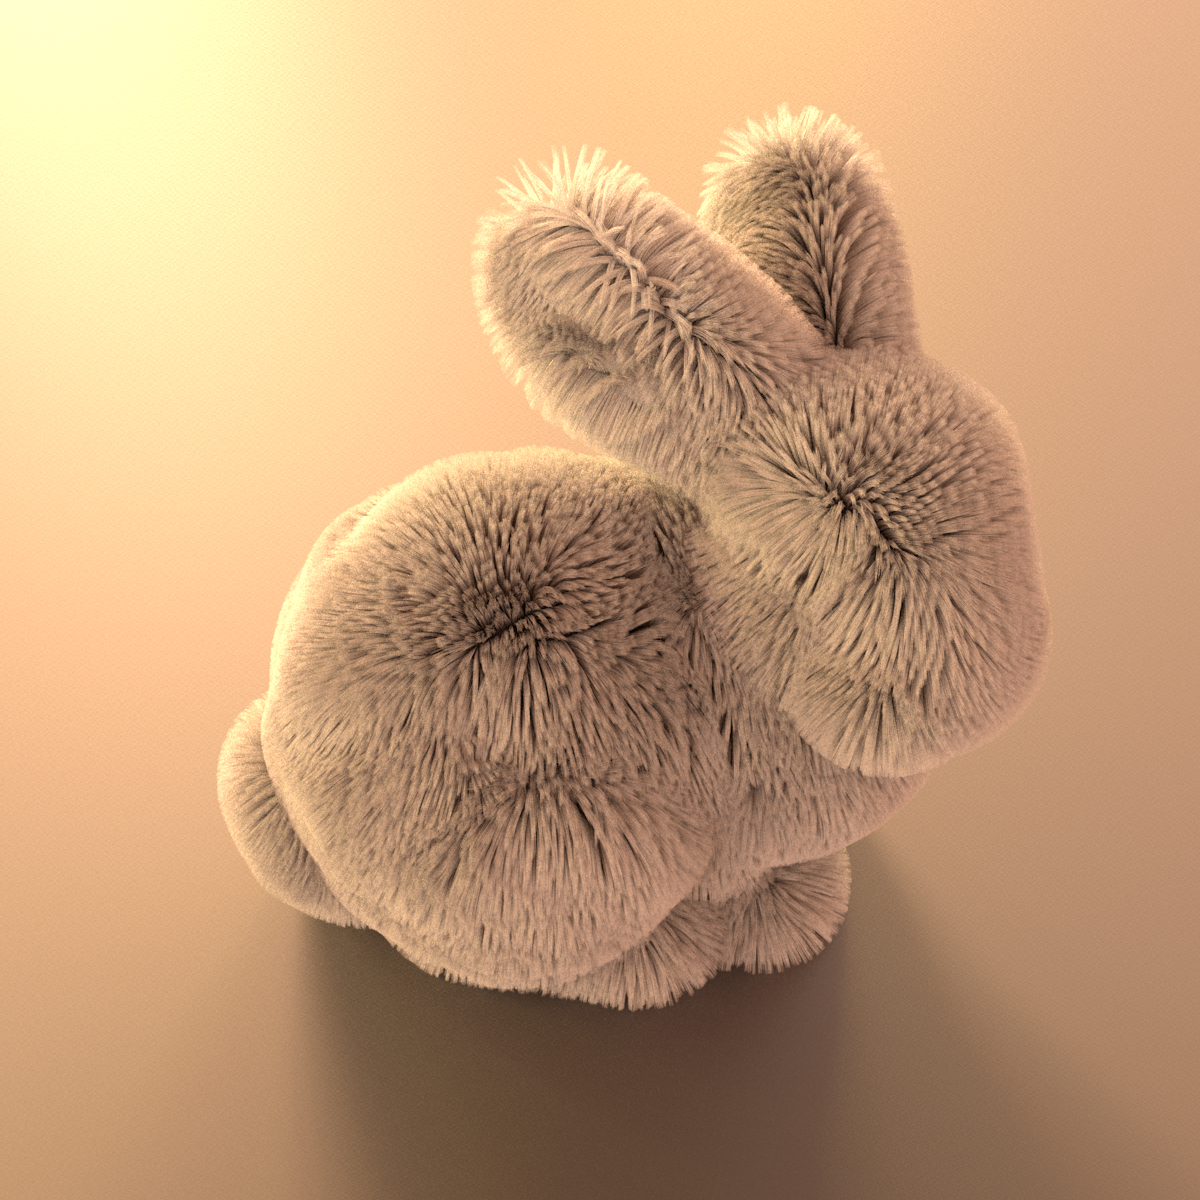
\includegraphics[width=\linewidth]{chap03/furrybunny.png}
    \caption{毛茸茸的小兔子。上百万\refvar{Curve}{}形状用于建模皮毛的小兔子模型。
        这里我们使用了不真实的长曲线来更好展示\refvar{Curve}{}的能力。}
    \label{fig:3.17}
\end{figure}
\begin{lstlisting}
`\initcode{CurveDeclarations}{=}`
class `\initvar{Curve}{}` : public `\refvar{Shape}{}` {
public:
    `\refcode{Curve Public Methods}{}`
private:
    `\refcode{Curve Private Methods}{}`
    `\refcode{Curve Private Data}{}`
};
\end{lstlisting}
\begin{lstlisting}
`\initcode{Curve Private Methods}{=}`
bool `\refvar{recursiveIntersect}{}`(const `\refvar{Ray}{}` &r, `\refvar{Float}{}` *tHit,
    `\refvar{SurfaceInteraction}{}` *isect, const `\refvar{Point3f}{}` cp[4],
    const `\refvar{Transform}{}` &rayToObject, `\refvar{Float}{}` u0, `\refvar{Float}{}` u1, int depth) const;

\end{lstlisting}

如\reffig{3.18}所示,\refvar{Curve}{}形状可以表示三种曲线。
\begin{itemize}
    \item \keyindex{平坦面}{flat}{}:这种表示的曲线总是朝向与之相交的光线;
          它们在建模细微扫掠圆柱形状如头发或皮毛时很有用。
    \item {\sffamily 圆柱}:对于在屏幕上张开几像素的曲线(如不远处看到的意大利面),
          \refvar{Curve}{}形状可以计算着色法线使得曲线看起来实际是圆柱体。
    \item \keyindex{丝带}{ribbon}{}:这个变体对于建模实际没有
          圆柱\keyindex{横截面}{cross section}{}的形状(例如一片草)很有用。
\end{itemize}
\begin{figure}[htbp]
    \centering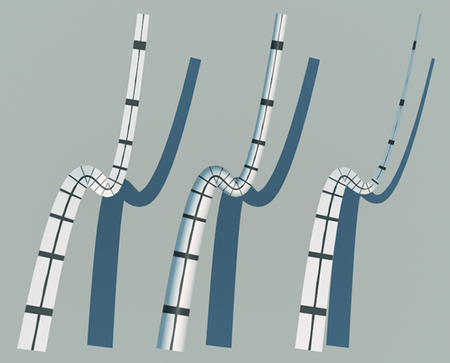
\includegraphics[width=0.5\linewidth]{chap03/threecurves.png}
    \caption{\protect\refvar{Curve}{}形状可以表示的三种曲线。
        左边是平坦曲线,总是朝向垂直于光线接近它的方向。
        中间的变体可以设置着色法线使得曲线看起来是圆柱体。
        右边是丝带,在起点和终点有固定朝向;中间的朝向在它们之间平滑插值。}
    \label{fig:3.18}
\end{figure}

枚举\refvar{CurveType}{}记录了给定的\refvar{Curve}{}实例模型是它们中的哪一个。

平坦和圆柱曲线变体旨在用于方便地近似变形的圆柱体。
要注意的是针对它们求得的相交并不对应物理可实现的3D形状,
在拿真正的圆柱体场景作参考时这可能导致微小的矛盾。
\begin{lstlisting}
`\initcode{CurveType Declarations}{=}`
enum class `\initvar{CurveType}{}` { `\initvar{Flat}{}`, `\initvar[CurveType::Cylinder]{Cylinder}{}`, `\initvar{Ribbon}{}` };
\end{lstlisting}

给定在pbrt场景描述文件中指定的曲线,
值得将其分为若干段,每段包含曲线的一部分参数$u$范围。
(这样做的一个原因是轴对齐边界框不能紧致地包围起伏的曲线,
但把贝塞尔样条分开会使其不那么弯——
多项式样条的\keyindex{变差缩减性}{variation diminishing property}{}。)
因此,\refvar{Curve}{}构造函数同时
接收$u$值的参数范围$[u_{\min},u_{\max}]$以及
指向结构体\refvar{CurveCommon}{}的指针,
它存储了控制点和各曲线段共享的关于曲线的其他信息。
这样,单个曲线段所占内存被最小化,
使得在内存中保留许多曲线更容易。
\begin{lstlisting}
`\initcode{Curve Public Methods}{=}`
`\refvar{Curve}{}`(const `\refvar{Transform}{}` *ObjectToWorld, const `\refvar{Transform}{}` *WorldToObject,
      bool reverseOrientation, const std::shared_ptr<`\refvar{CurveCommon}{}`> &common,
      `\refvar{Float}{}` uMin, `\refvar{Float}{}` uMax)
    : `\refvar{Shape}{}`(ObjectToWorld, WorldToObject, reverseOrientation),
      `\refvar{common}{}`(common), `\refvar{uMin}{}`(uMin), `\refvar{uMax}{}`(uMax) { }
\end{lstlisting}
\begin{lstlisting}
`\initcode{Curve Private Data}{=}`
const std::shared_ptr<`\refvar{CurveCommon}{}`> `\initvar{common}{}`;
const `\refvar{Float}{}` `\initvar{uMin}{}`, `\initvar{uMax}{}`; 
\end{lstlisting}

\refvar{CurveCommon}{}构造函数大多数只初始化成员变量
和传入的控制点值、曲线宽度等。
提供给它的控制点应该在曲线的物体空间内。

对于\refvar{Ribbon}{}曲线,\refvar{CurveCommon}{}存储了
曲面法线以在每个终点处让曲线定向。
构造函数预计算两个法向量的夹角并求该角正弦的倒数;
这些值会在沿曲线范围计算任意点处的朝向时很有用。
\begin{lstlisting}
`\initcode{Curve Method Definitions}{=}\initnext{CurveMethodDefinitions}`
`\refvar{CurveCommon}{}`::`\refvar{CurveCommon}{}`(const `\refvar{Point3f}{}` c[4], `\refvar{Float}{}` width0, `\refvar{Float}{}` width1,
        `\refvar{CurveType}{}` type, const `\refvar{Normal3f}{}` *norm)
    : `\refvar[CurveCommon::type]{type}{}`(type), `\refvar{cpObj}{}`{c[0], c[1], c[2], c[3]},
      `\refvar[CurveCommon::width]{width}{}`{width0, width1} {
    if (norm) {
        `\refvar[CurveCommon::n]{n}{}`[0] = `\refvar{Normalize}{}`(norm[0]);
        `\refvar[CurveCommon::n]{n}{}`[1] = `\refvar{Normalize}{}`(norm[1]);
        `\refvar{normalAngle}{}` = std::acos(`\refvar{Clamp}{}`(`\refvar{Dot}{}`(`\refvar[CurveCommon::n]{n}{}`[0], `\refvar[CurveCommon::n]{n}{}`[1]), 0, 1));
        `\refvar{invSinNormalAngle}{}` = 1 / std::sin(`\refvar{normalAngle}{}`);
    }
}
\end{lstlisting}
\begin{lstlisting}
`\initcode{CurveCommon Declarations}{=}`
struct `\initvar{CurveCommon}{}` {
    const `\refvar{CurveType}{}` `\initvar[CurveCommon::type]{type}{}`;
    const `\refvar{Point3f}{}` `\initvar{cpObj}{}`[4];
    const `\refvar{Float}{}` `\initvar[CurveCommon::width]{width}{}`[2];
    `\refvar{Normal3f}{}` `\initvar[CurveCommon::n]{n}{}`[2];
    `\refvar{Float}{}` `\initvar{normalAngle}{}`, `\initvar{invSinNormalAngle}{}`;
};
\end{lstlisting}

\refvar{Curve}{}的边界框可通过利用\keyindex{凸包性质}{convex hull property}{convex hull凸包}计算,
这是贝塞尔曲线的性质,即它们一定位于其控制点的\keyindex{凸包}{convex hull}{}内
\sidenote{译者注:在实数向量空间中,对于给定集合$X$,
所有包含$X$的凸集的交集$S$称为$X$的凸包,
它可以用$X$内所有点$(x_1,\ldots,x_n)$的线性组合来构造,
即$\displaystyle S=\{\sum\limits_{j=1}^n{t_jx_j}|x_j\in X,\sum\limits_{j=1}^n{t_j}=1,t_j\in[0,1]\}$。}。
因此,控制点的边界框给出了底层曲线的保守边界。
方法\refvar[Curve::ObjectBound]{ObjectBound}{()}首先
计算1D贝塞尔段的控制点边界框来沿曲线的中心包围样条。
然后这些边界在曲线参数范围内被展开所取最大宽度的一半,
得到\refvar{Curve}{}表示的\refvar{Shape}{}的3D边界。
\begin{lstlisting}
`\refcode{Curve Method Definitions}{+=}\lastnext{CurveMethodDefinitions}`
`\refvar{Bounds3f}{}` `\initvar{Curve::ObjectBound}{}`() const {
    `\refcode{Compute object-space control points for curve segment, cpObj}{}`
    `\refvar{Bounds3f}{}` b = `\refvar[Union2]{Union}{}`(`\refvar{Bounds3f}{}`(cpObj[0], cpObj[1]),
                       `\refvar{Bounds3f}{}`(cpObj[2], cpObj[3]));
    `\refvar{Float}{}` width[2] = { `\refvar{Lerp}{}`(`\refvar{uMin}{}`, `\refvar{common}{}`->`\refvar[CurveCommon::width]{width}{}`[0], `\refvar{common}{}`->`\refvar[CurveCommon::width]{width}{}`[1]),
                       `\refvar{Lerp}{}`(`\refvar{uMax}{}`, `\refvar{common}{}`->`\refvar[CurveCommon::width]{width}{}`[0], `\refvar{common}{}`->`\refvar[CurveCommon::width]{width}{}`[1]) };
    return `\refvar{Expand}{}`(b, std::max(width[0], width[1]) * 0.5f);
}
\end{lstlisting}

类\refvar{CurveCommon}{}存储了整条曲线的控制点,
但\refvar{Curve}{}实例通常需要对应其$u$范围的
表示贝塞尔曲线的四个控制点。
这些控制点用称为\keyindex{开花}{blossoming}{}的技术计算。
三次贝塞尔样条簇\sidenote{译者注:原文blossom。}$\bm p(u_0,u_1,u_2)$由三个阶段的线性插值定义,
从原始控制点开始:
\begin{align}\label{eq:3.4}
    \bm a_i & =(1-u_0)\bm p_i+u_0\bm p_{i+1},\quad i\in[0,1,2]\nonumber\, , \\
    \bm b_j & =(1-u_1)\bm a_j+u_1\bm a_{j+1},\quad j\in[0,1]\nonumber\, ,   \\
    \bm c   & =(1-u_2)\bm b_0+u_2\bm b_1\, .
\end{align}

簇$\bm p(u,u,u)$给出了在位置$u$处的曲线值
(要自己验证的话,用$u_i=u$展开\refeq{3.4},化简,并和\refeq{3.3}比较)。

\refvar{BlossomBezier}{()}实现了该计算。
\begin{lstlisting}
`\initcode{Curve Utility Functions}{=}\initnext{CurveUtilityFunctions}`
static `\refvar{Point3f}{}` `\initvar{BlossomBezier}{}`(const `\refvar{Point3f}{}` p[4], `\refvar{Float}{}` u0, `\refvar{Float}{}` u1,
        `\refvar{Float}{}` u2) {
    `\refvar{Point3f}{}` a[3] = { `\refvar{Lerp}{}`(u0, p[0], p[1]),
                     `\refvar{Lerp}{}`(u0, p[1], p[2]),
                     `\refvar{Lerp}{}`(u0, p[2], p[3]) };
    `\refvar{Point3f}{}` b[2] = { `\refvar{Lerp}{}`(u1, a[0], a[1]), `\refvar{Lerp}{}`(u1, a[1], a[2]) };
    return `\refvar{Lerp}{}`(u2, b[0], b[1]);
}
\end{lstlisting}
\begin{figure}[htbp]
    \centering%LaTeX with PSTricks extensions
%%Creator: Inkscape 1.0.1 (3bc2e813f5, 2020-09-07)
%%Please note this file requires PSTricks extensions
\psset{xunit=.32pt,yunit=.32pt,runit=.32pt}
\begin{pspicture}(465.62508138,170.46652222)
{
\newrgbcolor{curcolor}{0 0 0}
\pscustom[linewidth=1.33333336,linecolor=curcolor]
{
\newpath
\moveto(1.60947576,70.53795366)
\curveto(154.78134799,223.70983522)(384.541779,-82.6339159)(461.13031379,147.12650044)
}
}
{
\newrgbcolor{curcolor}{0 0 0}
\pscustom[linewidth=2.66666672,linecolor=curcolor]
{
\newpath
\moveto(260.08864332,80.11087384)
\curveto(346.25011161,51.39212663)(422.83864639,32.24628627)(461.13031379,147.12650044)
}
}
{
\newrgbcolor{curcolor}{0 0 0}
\pscustom[linestyle=none,fillstyle=solid,fillcolor=curcolor]
{
\newpath
\moveto(263.62511005,79.56920716)
\curveto(263.62511005,80.52232718)(263.25011004,81.43379387)(262.5730167,82.10566055)
\curveto(261.90115002,82.78275389)(260.98968333,83.1577539)(260.03656332,83.1577539)
\curveto(259.0834433,83.1577539)(258.17197661,82.78275389)(257.50010994,82.10566055)
\curveto(256.82301659,81.43379387)(256.44801658,80.52232718)(256.44801658,79.56920716)
\curveto(256.44801658,78.61608715)(256.82301659,77.70462046)(257.50010994,77.03275378)
\curveto(258.17197661,76.35566044)(259.0834433,75.98066043)(260.03656332,75.98066043)
\curveto(260.98968333,75.98066043)(261.90115002,76.35566044)(262.5730167,77.03275378)
\curveto(263.25011004,77.70462046)(263.62511005,78.61608715)(263.62511005,79.56920716)
\closepath
\moveto(263.62511005,79.56920716)
}
}
{
\newrgbcolor{curcolor}{0 0 0}
\pscustom[linestyle=none,fillstyle=solid,fillcolor=curcolor]
{
\newpath
\moveto(350.29177836,51.56920664)
\curveto(350.29177836,52.52232665)(349.91677835,53.43379334)(349.239685,54.10566002)
\curveto(348.56781832,54.78275336)(347.65635164,55.15775337)(346.70323162,55.15775337)
\curveto(345.7501116,55.15775337)(344.83864492,54.78275336)(344.16677824,54.10566002)
\curveto(343.48968489,53.43379334)(343.11468489,52.52232665)(343.11468489,51.56920664)
\curveto(343.11468489,50.61608662)(343.48968489,49.70461993)(344.16677824,49.03275325)
\curveto(344.83864492,48.35565991)(345.7501116,47.9806599)(346.70323162,47.9806599)
\curveto(347.65635164,47.9806599)(348.56781832,48.35565991)(349.239685,49.03275325)
\curveto(349.91677835,49.70461993)(350.29177836,50.61608662)(350.29177836,51.56920664)
\closepath
\moveto(350.29177836,51.56920664)
}
}
{
\newrgbcolor{curcolor}{0 0 0}
\pscustom[linestyle=none,fillstyle=solid,fillcolor=curcolor]
{
\newpath
\moveto(426.29177979,32.90253962)
\curveto(426.29177979,33.85565963)(425.91677979,34.76712632)(425.23968644,35.438993)
\curveto(424.56781976,36.11608634)(423.65635308,36.49108635)(422.70323306,36.49108635)
\curveto(421.75011304,36.49108635)(420.83864636,36.11608634)(420.16677968,35.438993)
\curveto(419.48968633,34.76712632)(419.11468632,33.85565963)(419.11468632,32.90253962)
\curveto(419.11468632,31.9494196)(419.48968633,31.03795291)(420.16677968,30.36608623)
\curveto(420.83864636,29.68899289)(421.75011304,29.31399288)(422.70323306,29.31399288)
\curveto(423.65635308,29.31399288)(424.56781976,29.68899289)(425.23968644,30.36608623)
\curveto(425.91677979,31.03795291)(426.29177979,31.9494196)(426.29177979,32.90253962)
\closepath
\moveto(426.29177979,32.90253962)
}
}
{
\newrgbcolor{curcolor}{0 0 0}
\pscustom[linestyle=none,fillstyle=solid,fillcolor=curcolor]
{
\newpath
\moveto(464.95844719,147.56920845)
\curveto(464.95844719,148.5223338)(464.58344718,149.43379249)(463.90635384,150.10566717)
\curveto(463.23448716,150.78274984)(462.32302047,151.15774985)(461.36990046,151.15774985)
\curveto(460.41678044,151.15774985)(459.50531375,150.78274984)(458.83344708,150.10566717)
\curveto(458.15635373,149.43379249)(457.78135372,148.5223338)(457.78135372,147.56920845)
\curveto(457.78135372,146.6160831)(458.15635373,145.70462442)(458.83344708,145.03274974)
\curveto(459.50531375,144.35566706)(460.41678044,143.98066705)(461.36990046,143.98066705)
\curveto(462.32302047,143.98066705)(463.23448716,144.35566706)(463.90635384,145.03274974)
\curveto(464.58344718,145.70462442)(464.95844719,146.6160831)(464.95844719,147.56920845)
\closepath
\moveto(464.95844719,147.56920845)
}
}
{
\newrgbcolor{curcolor}{0 0 0}
\pscustom[linestyle=none,fillstyle=solid,fillcolor=curcolor]
{
\newpath
\moveto(427.14892288,154.38318208)
\curveto(427.06558955,154.00818207)(427.02392288,153.96651541)(426.98225621,153.92484874)
\curveto(426.85725621,153.88318207)(426.56558954,153.88318207)(426.31558953,153.88318207)
\curveto(425.85725619,153.88318207)(425.35725618,153.88318207)(425.35725618,153.13318206)
\curveto(425.35725618,152.84151539)(425.60725619,152.63318205)(425.89892286,152.63318205)
\curveto(426.64892287,152.63318205)(427.52392289,152.71651538)(428.31558957,152.71651538)
\curveto(429.27392292,152.71651538)(430.27392294,152.63318205)(431.19058962,152.63318205)
\curveto(431.35725629,152.63318205)(431.8572563,152.63318205)(431.8572563,153.42484873)
\curveto(431.8572563,153.88318207)(431.44058963,153.88318207)(431.19058962,153.88318207)
\curveto(430.81558962,153.88318207)(430.35725628,153.88318207)(430.02392294,153.92484874)
\lineto(431.19058962,158.54984883)
\curveto(431.56558963,158.17484882)(432.44058965,157.59151548)(433.85725634,157.59151548)
\curveto(438.48225643,157.59151548)(441.35725648,161.79984889)(441.35725648,165.42484896)
\curveto(441.35725648,168.71651569)(438.8989231,169.79984904)(436.69058973,169.79984904)
\curveto(434.81558969,169.79984904)(433.44058967,168.75818235)(433.02392299,168.38318235)
\curveto(431.98225631,169.79984904)(430.23225627,169.79984904)(429.9405896,169.79984904)
\curveto(428.98225625,169.79984904)(428.19058957,169.25818236)(427.64892289,168.29984901)
\curveto(426.98225621,167.21651566)(426.6072562,165.79984896)(426.6072562,165.67484896)
\curveto(426.6072562,165.29984896)(427.02392288,165.29984896)(427.27392288,165.29984896)
\curveto(427.56558956,165.29984896)(427.64892289,165.29984896)(427.77392289,165.42484896)
\curveto(427.85725623,165.46651562)(427.85725623,165.54984896)(428.0239229,166.21651564)
\curveto(428.52392291,168.34151568)(429.14892292,168.84151569)(429.8155896,168.84151569)
\curveto(430.10725627,168.84151569)(430.44058961,168.75818235)(430.44058961,167.88318234)
\curveto(430.44058961,167.46651566)(430.35725628,167.09151566)(430.27392294,166.71651565)
\closepath
\moveto(433.273923,167.13318232)
\curveto(434.02392301,168.04984901)(435.27392303,168.84151569)(436.56558973,168.84151569)
\curveto(438.23225642,168.84151569)(438.35725643,167.424849)(438.35725643,166.84151565)
\curveto(438.35725643,165.46651562)(437.44058974,162.1748489)(437.02392307,161.13318221)
\curveto(436.19058972,159.21651551)(434.89892303,158.54984883)(433.81558967,158.54984883)
\curveto(432.23225631,158.54984883)(431.6072563,159.79984885)(431.6072563,160.09151552)
\lineto(431.64892297,160.46651553)
\closepath
\moveto(433.273923,167.13318232)
}
}
{
\newrgbcolor{curcolor}{0 0 0}
\pscustom[linestyle=none,fillstyle=solid,fillcolor=curcolor]
{
\newpath
\moveto(446.82258862,160.0241734)
\curveto(448.28092198,160.0241734)(449.32258866,159.02417338)(449.32258866,157.02417334)
\curveto(449.32258866,154.73250663)(447.94758864,154.02417329)(446.90592195,154.02417329)
\curveto(446.15592194,154.02417329)(444.48925524,154.23250662)(443.73925523,155.35750664)
\curveto(444.61425524,155.35750664)(444.82258858,155.98250666)(444.82258858,156.39917333)
\curveto(444.82258858,156.98250668)(444.36425524,157.39917335)(443.78092189,157.39917335)
\curveto(443.28092188,157.39917335)(442.73925521,157.06584001)(442.73925521,156.31584)
\curveto(442.73925521,154.56583996)(444.65592191,153.44083994)(446.90592195,153.44083994)
\curveto(449.48925533,153.44083994)(451.28092204,155.19083997)(451.28092204,157.02417334)
\curveto(451.28092204,158.4825067)(450.11425535,159.94084006)(448.07258864,160.35750674)
\curveto(449.98925534,161.06584009)(450.69758869,162.44084011)(450.69758869,163.6075068)
\curveto(450.69758869,165.06584016)(449.03092199,166.14917352)(446.94758862,166.14917352)
\curveto(444.90592191,166.14917352)(443.32258855,165.1491735)(443.32258855,163.64917347)
\curveto(443.32258855,163.02417346)(443.73925523,162.69084012)(444.2809219,162.69084012)
\curveto(444.86425525,162.69084012)(445.23925525,163.10750679)(445.23925525,163.6075068)
\curveto(445.23925525,164.14917348)(444.86425525,164.56584015)(444.2809219,164.60750682)
\curveto(444.94758858,165.3991735)(446.19758861,165.60750684)(446.90592195,165.60750684)
\curveto(447.7392553,165.60750684)(448.90592199,165.19084016)(448.90592199,163.6075068)
\curveto(448.90592199,162.81584012)(448.65592199,161.9408401)(448.15592198,161.39917343)
\curveto(447.57258863,160.69084008)(447.03092195,160.64917341)(446.11425527,160.56584008)
\curveto(445.65592193,160.52417341)(445.61425526,160.52417341)(445.53092193,160.52417341)
\curveto(445.48925526,160.52417341)(445.32258859,160.48250674)(445.32258859,160.2741734)
\curveto(445.32258859,160.0241734)(445.48925526,160.0241734)(445.8225886,160.0241734)
\closepath
\moveto(446.82258862,160.0241734)
}
}
{
\newrgbcolor{curcolor}{0 0 0}
\pscustom[linestyle=none,fillstyle=solid,fillcolor=curcolor]
{
\newpath
\moveto(411.75142926,2.41665921)
\curveto(411.66809592,2.0416592)(411.62642925,1.99999253)(411.58476259,1.95832587)
\curveto(411.45976258,1.9166592)(411.16809591,1.9166592)(410.91809591,1.9166592)
\curveto(410.45976257,1.9166592)(409.95976256,1.9166592)(409.95976256,1.16665918)
\curveto(409.95976256,0.87499251)(410.20976256,0.66665918)(410.50142923,0.66665918)
\curveto(411.25142925,0.66665918)(412.12642926,0.74999251)(412.91809595,0.74999251)
\curveto(413.8764293,0.74999251)(414.87642932,0.66665918)(415.793096,0.66665918)
\curveto(415.95976267,0.66665918)(416.45976268,0.66665918)(416.45976268,1.45832586)
\curveto(416.45976268,1.9166592)(416.043096,1.9166592)(415.793096,1.9166592)
\curveto(415.41809599,1.9166592)(414.95976265,1.9166592)(414.62642931,1.95832587)
\lineto(415.793096,6.58332595)
\curveto(416.16809601,6.20832595)(417.04309602,5.6249926)(418.45976272,5.6249926)
\curveto(423.0847628,5.6249926)(425.95976286,9.83332602)(425.95976286,13.45832608)
\curveto(425.95976286,16.74999281)(423.50142948,17.83332617)(421.2930961,17.83332617)
\curveto(419.41809607,17.83332617)(418.04309604,16.79165948)(417.62642937,16.41665947)
\curveto(416.58476268,17.83332617)(414.83476265,17.83332617)(414.54309598,17.83332617)
\curveto(413.58476262,17.83332617)(412.79309594,17.29165949)(412.25142927,16.33332614)
\curveto(411.58476259,15.24999278)(411.20976258,13.83332609)(411.20976258,13.70832609)
\curveto(411.20976258,13.33332608)(411.62642925,13.33332608)(411.87642926,13.33332608)
\curveto(412.16809593,13.33332608)(412.25142927,13.33332608)(412.37642927,13.45832608)
\curveto(412.4597626,13.49999275)(412.4597626,13.58332609)(412.62642927,14.24999277)
\curveto(413.12642928,16.37499281)(413.75142929,16.87499282)(414.41809597,16.87499282)
\curveto(414.70976265,16.87499282)(415.04309599,16.79165948)(415.04309599,15.91665946)
\curveto(415.04309599,15.49999279)(414.95976265,15.12499278)(414.87642932,14.74999278)
\closepath
\moveto(417.87642937,15.16665945)
\curveto(418.62642939,16.08332613)(419.87642941,16.87499282)(421.1680961,16.87499282)
\curveto(422.8347628,16.87499282)(422.9597628,15.45832612)(422.9597628,14.87499278)
\curveto(422.9597628,13.49999275)(422.04309612,10.20832602)(421.62642944,9.16665934)
\curveto(420.79309609,7.24999263)(419.5014294,6.58332595)(418.41809605,6.58332595)
\curveto(416.83476269,6.58332595)(416.20976267,7.83332598)(416.20976267,8.12499265)
\lineto(416.25142934,8.49999266)
\closepath
\moveto(417.87642937,15.16665945)
}
}
{
\newrgbcolor{curcolor}{0 0 0}
\pscustom[linestyle=none,fillstyle=solid,fillcolor=curcolor]
{
\newpath
\moveto(435.71676174,5.22431714)
\lineto(435.09176173,5.22431714)
\curveto(435.05009506,4.80765046)(434.84176172,3.72431711)(434.59176172,3.55765044)
\curveto(434.46676172,3.43265044)(433.05009502,3.43265044)(432.75842835,3.43265044)
\lineto(429.34176162,3.43265044)
\curveto(431.30009499,5.1409838)(431.96676167,5.68265048)(433.05009502,6.5576505)
\curveto(434.42509505,7.64098385)(435.71676174,8.80765054)(435.71676174,10.55765057)
\curveto(435.71676174,12.80765062)(433.75842837,14.18265064)(431.38342833,14.18265064)
\curveto(429.09176162,14.18265064)(427.50842825,12.55765061)(427.50842825,10.84931725)
\curveto(427.50842825,9.93265056)(428.30009493,9.80765056)(428.50842827,9.80765056)
\curveto(428.92509495,9.80765056)(429.46676162,10.1409839)(429.46676162,10.80765058)
\curveto(429.46676162,11.14098392)(429.34176162,11.8076506)(428.38342827,11.8076506)
\curveto(428.96676161,13.09931729)(430.21676164,13.51598396)(431.09176165,13.51598396)
\curveto(432.96676169,13.51598396)(433.92509504,12.0576506)(433.92509504,10.55765057)
\curveto(433.92509504,8.93265054)(432.75842835,7.68265052)(432.17509501,7.01598384)
\lineto(427.71676159,2.55765042)
\curveto(427.50842825,2.39098375)(427.50842825,2.34931708)(427.50842825,1.84931708)
\lineto(435.17509506,1.84931708)
\closepath
\moveto(435.71676174,5.22431714)
}
}
{
\newrgbcolor{curcolor}{0 0 0}
\pscustom[linestyle=none,fillstyle=solid,fillcolor=curcolor]
{
\newpath
\moveto(334.76397447,21.83088624)
\curveto(334.68064113,21.45588624)(334.63897447,21.41421957)(334.5973078,21.3725529)
\curveto(334.4723078,21.33088623)(334.18064112,21.33088623)(333.93064112,21.33088623)
\curveto(333.47230778,21.33088623)(332.97230777,21.33088623)(332.97230777,20.58088622)
\curveto(332.97230777,20.28921955)(333.22230777,20.08088621)(333.51397444,20.08088621)
\curveto(334.26397446,20.08088621)(335.13897447,20.16421954)(335.93064116,20.16421954)
\curveto(336.88897451,20.16421954)(337.88897453,20.08088621)(338.80564121,20.08088621)
\curveto(338.97230788,20.08088621)(339.47230789,20.08088621)(339.47230789,20.87255289)
\curveto(339.47230789,21.33088623)(339.05564122,21.33088623)(338.80564121,21.33088623)
\curveto(338.4306412,21.33088623)(337.97230786,21.33088623)(337.63897452,21.3725529)
\lineto(338.80564121,25.99755299)
\curveto(339.18064122,25.62255298)(340.05564123,25.03921964)(341.47230793,25.03921964)
\curveto(346.09730802,25.03921964)(348.97230807,29.24755305)(348.97230807,32.87255312)
\curveto(348.97230807,36.16421985)(346.51397469,37.2475532)(344.30564131,37.2475532)
\curveto(342.43064128,37.2475532)(341.05564125,36.20588651)(340.63897458,35.83088651)
\curveto(339.59730789,37.2475532)(337.84730786,37.2475532)(337.55564119,37.2475532)
\curveto(336.59730784,37.2475532)(335.80564115,36.70588652)(335.26397448,35.74755317)
\curveto(334.5973078,34.66421982)(334.22230779,33.24755312)(334.22230779,33.12255312)
\curveto(334.22230779,32.74755312)(334.63897447,32.74755312)(334.88897447,32.74755312)
\curveto(335.18064114,32.74755312)(335.26397448,32.74755312)(335.38897448,32.87255312)
\curveto(335.47230781,32.91421979)(335.47230781,32.99755312)(335.63897448,33.6642198)
\curveto(336.13897449,35.78921984)(336.76397451,36.28921985)(337.43064118,36.28921985)
\curveto(337.72230786,36.28921985)(338.0556412,36.20588651)(338.0556412,35.3308865)
\curveto(338.0556412,34.91421982)(337.97230786,34.53921982)(337.88897453,34.16421981)
\closepath
\moveto(340.88897458,34.58088648)
\curveto(341.6389746,35.49755317)(342.88897462,36.28921985)(344.18064131,36.28921985)
\curveto(345.84730801,36.28921985)(345.97230801,34.87255316)(345.97230801,34.28921981)
\curveto(345.97230801,32.91421979)(345.05564133,29.62255306)(344.63897465,28.58088637)
\curveto(343.80564131,26.66421967)(342.51397461,25.99755299)(341.43064126,25.99755299)
\curveto(339.8473079,25.99755299)(339.22230789,27.24755301)(339.22230789,27.53921968)
\lineto(339.26397455,27.91421969)
\closepath
\moveto(340.88897458,34.58088648)
}
}
{
\newrgbcolor{curcolor}{0 0 0}
\pscustom[linestyle=none,fillstyle=solid,fillcolor=curcolor]
{
\newpath
\moveto(355.56264023,33.09687767)
\curveto(355.56264023,33.59687768)(355.56264023,33.59687768)(355.02097355,33.59687768)
\curveto(353.81264019,32.43021099)(352.14597349,32.43021099)(351.39597348,32.43021099)
\lineto(351.39597348,31.76354431)
\curveto(351.81264015,31.76354431)(353.06264018,31.76354431)(354.0626402,32.26354432)
\lineto(354.0626402,22.80521081)
\curveto(354.0626402,22.18021079)(354.0626402,21.93021079)(352.22930683,21.93021079)
\lineto(351.52097348,21.93021079)
\lineto(351.52097348,21.26354411)
\curveto(351.85430682,21.26354411)(354.14597353,21.34687744)(354.81264021,21.34687744)
\curveto(355.39597356,21.34687744)(357.72930693,21.26354411)(358.14597361,21.26354411)
\lineto(358.14597361,21.93021079)
\lineto(357.43764026,21.93021079)
\curveto(355.56264023,21.93021079)(355.56264023,22.18021079)(355.56264023,22.80521081)
\closepath
\moveto(355.56264023,33.09687767)
}
}
{
\newrgbcolor{curcolor}{0 0 0}
\pscustom[linestyle=none,fillstyle=solid,fillcolor=curcolor]
{
\newpath
\moveto(247.06522653,44.59239334)
\curveto(246.98189319,44.21739333)(246.94022653,44.17572666)(246.89855986,44.13406)
\curveto(246.77355986,44.09239333)(246.48189319,44.09239333)(246.23189318,44.09239333)
\curveto(245.77355984,44.09239333)(245.27355983,44.09239333)(245.27355983,43.34239332)
\curveto(245.27355983,43.05072664)(245.52355983,42.84239331)(245.81522651,42.84239331)
\curveto(246.56522652,42.84239331)(247.44022654,42.92572664)(248.23189322,42.92572664)
\curveto(249.19022657,42.92572664)(250.19022659,42.84239331)(251.10689327,42.84239331)
\curveto(251.27355994,42.84239331)(251.77355995,42.84239331)(251.77355995,43.63405999)
\curveto(251.77355995,44.09239333)(251.35689328,44.09239333)(251.10689327,44.09239333)
\curveto(250.73189327,44.09239333)(250.27355992,44.09239333)(249.94022658,44.13406)
\lineto(251.10689327,48.75906008)
\curveto(251.48189328,48.38406008)(252.3568933,47.80072673)(253.77355999,47.80072673)
\curveto(258.39856008,47.80072673)(261.27356013,52.00906015)(261.27356013,55.63406021)
\curveto(261.27356013,58.92572694)(258.81522675,60.0090603)(256.60689338,60.0090603)
\curveto(254.73189334,60.0090603)(253.35689332,58.96739361)(252.94022664,58.5923936)
\curveto(251.89855995,60.0090603)(250.14855992,60.0090603)(249.85689325,60.0090603)
\curveto(248.8985599,60.0090603)(248.10689322,59.46739362)(247.56522654,58.50906027)
\curveto(246.89855986,57.42572692)(246.52355985,56.00906022)(246.52355985,55.88406022)
\curveto(246.52355985,55.50906021)(246.94022653,55.50906021)(247.19022653,55.50906021)
\curveto(247.4818932,55.50906021)(247.56522654,55.50906021)(247.69022654,55.63406021)
\curveto(247.77355988,55.67572688)(247.77355988,55.75906022)(247.94022655,56.4257269)
\curveto(248.44022656,58.55072694)(249.06522657,59.05072695)(249.73189325,59.05072695)
\curveto(250.02355992,59.05072695)(250.35689326,58.96739361)(250.35689326,58.09239359)
\curveto(250.35689326,57.67572692)(250.27355992,57.30072691)(250.19022659,56.92572691)
\closepath
\moveto(253.19022665,57.34239358)
\curveto(253.94022666,58.25906026)(255.19022668,59.05072695)(256.48189337,59.05072695)
\curveto(258.14856007,59.05072695)(258.27356007,57.63406025)(258.27356007,57.05072691)
\curveto(258.27356007,55.67572688)(257.35689339,52.38406015)(256.94022672,51.34239347)
\curveto(256.10689337,49.42572676)(254.81522668,48.75906008)(253.73189332,48.75906008)
\curveto(252.14855996,48.75906008)(251.52355995,50.00906011)(251.52355995,50.30072678)
\lineto(251.56522661,50.67572679)
\closepath
\moveto(253.19022665,57.34239358)
}
}
{
\newrgbcolor{curcolor}{0 0 0}
\pscustom[linestyle=none,fillstyle=solid,fillcolor=curcolor]
{
\newpath
\moveto(271.23889235,49.94171798)
\curveto(271.23889235,51.98338469)(270.98889235,53.48338472)(270.155559,54.77505141)
\curveto(269.57222565,55.60838476)(268.40555896,56.35838477)(266.9472256,56.35838477)
\curveto(262.61389219,56.35838477)(262.61389219,51.27505134)(262.61389219,49.94171798)
\curveto(262.61389219,48.60838463)(262.61389219,43.6500512)(266.9472256,43.6500512)
\curveto(271.23889235,43.6500512)(271.23889235,48.60838463)(271.23889235,49.94171798)
\closepath
\moveto(266.9472256,44.19171788)
\curveto(266.07222559,44.19171788)(264.94722557,44.69171789)(264.57222556,46.19171791)
\curveto(264.32222555,47.27505127)(264.32222555,48.81671796)(264.32222555,50.19171799)
\curveto(264.32222555,51.56671802)(264.32222555,52.98338471)(264.57222556,53.98338473)
\curveto(264.98889223,55.44171809)(266.15555892,55.85838476)(266.9472256,55.85838476)
\curveto(267.94722562,55.85838476)(268.90555897,55.23338475)(269.23889231,54.1500514)
\curveto(269.53055899,53.15005138)(269.57222565,51.81671802)(269.57222565,50.19171799)
\curveto(269.57222565,48.81671796)(269.57222565,47.44171794)(269.32222565,46.27505125)
\curveto(268.94722564,44.56671788)(267.69722562,44.19171788)(266.9472256,44.19171788)
\closepath
\moveto(266.9472256,44.19171788)
}
}
\end{pspicture}

    \caption{一段贝塞尔曲线开花求控制点。
        \protect\refeq{3.5}中四簇给出从$u_{\min}$到$u_{\max}$的曲线控制点。
        开花提供了优雅方法计算整条曲线的子集曲线的贝塞尔控制点。}
    \label{fig:3.19}
\end{figure}

范围从$u_{\min}$到$u_{\max}$的曲线段的四个控制点由簇给出
\sidenote{译者注:通过繁琐但没有技巧性的多项式代换可以证明:
对于由控制点集$A=\{\bm p_i\}_{i=0}^3$定义的
三次贝塞尔样条簇$\bm p_A(u_0,u_1,u_2)$,
其中任意截取$u_j\in[u_j^0,u_j^1],j=0,1,2$,
并设$u_j^k(i)=\left\{\begin{array}{l}
        u_j^0,\ \text{若}i<k, \\
        u_j^1,\ \text{其他},
    \end{array}\right.$
然后取新控制点集$B=\{\bm q_i\}_{i=0}^3$,
其中$\bm q_i=\bm p(u_0^3(i),u_1^2(i),u_2^1(i))$,
并设新参数变量$\displaystyle v_j=\frac{u_j-u_j^0}{u_j^1-u_j^0}$,
则有$\bm p_B(v_0,v_1,v_2)\equiv\bm p_A(u_0,u_1,u_2)$,
即实现控制点集$A$到$B$的等价变换。}(\reffig{3.19}):
\begin{align}\label{eq:3.5}
    \bm p_0 & =\bm p(u_{\min},u_{\min},u_{\min})\nonumber\, , \\
    \bm p_1 & =\bm p(u_{\min},u_{\min},u_{\max})\nonumber\, , \\
    \bm p_2 & =\bm p(u_{\min},u_{\max},u_{\max})\nonumber\, , \\
    \bm p_3 & =\bm p(u_{\max},u_{\max},u_{\max})\, .
\end{align}

有了该机制,计算\refvar{Curve}{}负责的曲线段的四个控制点很简单。
\begin{lstlisting}
`\initcode{Compute object-space control points for curve segment, cpObj}{=}`
`\refvar{Point3f}{}` cpObj[4];
cpObj[0] = `\refvar{BlossomBezier}{}`(`\refvar{common}{}`->`\refvar{cpObj}{}`, `\refvar{uMin}{}`, `\refvar{uMin}{}`, `\refvar{uMin}{}`);
cpObj[1] = `\refvar{BlossomBezier}{}`(`\refvar{common}{}`->`\refvar{cpObj}{}`, `\refvar{uMin}{}`, `\refvar{uMin}{}`, `\refvar{uMax}{}`);
cpObj[2] = `\refvar{BlossomBezier}{}`(`\refvar{common}{}`->`\refvar{cpObj}{}`, `\refvar{uMin}{}`, `\refvar{uMax}{}`, `\refvar{uMax}{}`);
cpObj[3] = `\refvar{BlossomBezier}{}`(`\refvar{common}{}`->`\refvar{cpObj}{}`, `\refvar{uMax}{}`, `\refvar{uMax}{}`, `\refvar{uMax}{}`);
\end{lstlisting}

\refvar{Curve}{}相交算法基于尽快抛弃可以确定一定不会与光线相交的曲线段,
否则就递归地将曲线对半分为更小的两个曲线段然后再测试。
最终,曲线被线性近似以进行高效相交测试。
在一些准备工作后,\refvar{recursiveIntersect}{()}调用
使用\refvar{Curve}{}表示的整段曲线启动该进程。
\begin{lstlisting}
`\refcode{Curve Method Definitions}{+=}\lastnext{CurveMethodDefinitions}`
bool `\refvar{Curve}{}`::`\initvar[Curve::Intersect]{\refvar[Shape::Intersect]{Intersect}{}}{}`(const `\refvar{Ray}{}` &r, `\refvar{Float}{}` *tHit,
        `\refvar{SurfaceInteraction}{}` *isect, bool testAlphaTexture) const {
    `\refcode{Transform Ray to object space}{}`
    `\refcode{Compute object-space control points for curve segment, cpObj}{}`
    `\refcode{Project curve control points to plane perpendicular to ray}{}`
    `\refcode{Compute refinement depth for curve, maxDepth}{}`
    return `\refvar{recursiveIntersect}{}`(ray, tHit, isect, cp, `\refvar[Transform::Inverse]{Inverse}{}`(objectToRay),
                              `\refvar{uMin}{}`, `\refvar{uMax}{}`, maxDepth);
}
\end{lstlisting}

如同\refsub{三角形相交}的光线-三角形相交算法,
光线-曲线相交测试基于把曲线变换到射线端点在原点、
射线方向对齐$+z$轴的坐标系统。
一开始就执行该变换极大减少了相交测试必须执行的运算量。

对于\refvar{Curve}{}形状,我们需要变换的显式表示,
所以这里用函数\refvar{LookAt}{()}来生成它。
原点是射线的端点,“注视”点是从原点沿射线方向偏移的点,
“向上”方向是正交于射线方向的任意方向。
\begin{lstlisting}
`\initcode{Project curve control points to plane perpendicular to ray}{=}`
`\refvar{Vector3f}{}` dx, dy;
`\refvar{CoordinateSystem}{}`(ray.`\refvar[Ray::d]{d}{}`, &dx, &dy);
`\refvar{Transform}{}` objectToRay = `\refvar{LookAt}{}`(ray.`\refvar[Ray::o]{o}{}`, ray.`\refvar[Ray::o]{o}{}` + ray.`\refvar[Ray::d]{d}{}`, dx);
`\refvar{Point3f}{}` cp[4] = { objectToRay(cpObj[0]), objectToRay(cpObj[1]),
                  objectToRay(cpObj[2]), objectToRay(cpObj[3]) };
\end{lstlisting}

计算细分曲线的最大次数,这样与最精细级别的最终线性化曲线的距离
就被限定在小于某微小固定的距离内。
我们不深入该计算的细节
\sidenote{译者注:我对这段代码的理解是:
通过比较{\ttfamily cp[1]}与{\ttfamily cp[0]、cp[2]}的中点之差以及
{\ttfamily cp[2]}与{\ttfamily cp[1]、cp[3]}的中点之差,并取全部维度的最大绝对值,
{\ttfamily L0}表示了曲线的弯曲程度;{\ttfamily eps}表示最大宽度的一半。
{\ttfamily L0}与{\ttfamily eps}的比值反映了相应精度要求,
取对数后对应最大划分次数。},
它在代码片\refcode{Compute refinement depth for curve, maxDepth}{}中实现。
\begin{lstlisting}
`\initcode{Compute refinement depth for curve, maxDepth}{=}`
`\refvar{Float}{}` L0 = 0;
for (int i = 0; i < 2; ++i)
    L0 = std::max(L0,
         std::max(std::max(std::abs(cp[i].x - 2 * cp[i + 1].x + cp[i + 2].x),
                           std::abs(cp[i].y - 2 * cp[i + 1].y + cp[i + 2].y)),
                  std::abs(cp[i].z - 2 * cp[i + 1].z + cp[i + 2].z)));
`\refvar{Float}{}` eps = std::max(`\refvar{common}{}`->`\refvar[CurveCommon::width]{width}{}`[0], `\refvar{common}{}`->`\refvar[CurveCommon::width]{width}{}`[1]) * .05f; // width / 20
#define LOG4(x) (std::log(x) * 0.7213475108f)
`\refvar{Float}{}` fr0 = LOG4(1.41421356237f * 12.f * L0 / (8.f * eps));
#undef LOG4
int r0 = (int)std::round(fr0);
int maxDepth = `\refvar{Clamp}{}`(r0, 0, 10);
\end{lstlisting}

然后方法\refvar{recursiveIntersect}{()}测试给定射线是否与
在给定参数范围{\ttfamily [u0,u1]}内的曲线段相交。
\begin{lstlisting}
`\refcode{Curve Method Definitions}{+=}\lastcode{CurveMethodDefinitions}`
bool `\refvar{Curve}{}`::`\initvar{recursiveIntersect}{}`(const `\refvar{Ray}{}` &ray, `\refvar{Float}{}` *tHit,
        `\refvar{SurfaceInteraction}{}` *isect, const `\refvar{Point3f}{}` cp[4],
        const `\refvar{Transform}{}` &rayToObject, `\refvar{Float}{}` u0, `\refvar{Float}{}` u1,
        int depth) const {
    `\refcode{Try to cull curve segment versus ray}{}`
    if (depth > 0) {
        `\refcode{Split curve segment into sub-segments and test for intersection}{}`
    } else {
        `\refcode{Intersect ray with curve segment}{}`
    }
}
\end{lstlisting}

该方法先开始检查射线是否与曲线段的边界框相交;
如果没有,则不可能相交,它就立即返回。
\begin{lstlisting}
`\initcode{Try to cull curve segment versus ray}{=}`
`\refcode{Compute bounding box of curve segment, curveBounds}{}`
`\refcode{Compute bounding box of ray, rayBounds}{}`
if (`\refvar{Overlaps}{}`(curveBounds, rayBounds) == false)
    return false;
\end{lstlisting}

沿着\refvar{Curve::ObjectBound}{()}的实现路线,
可以通过接收曲线控制点的边界并在曲线考虑的$u$范围内
展开最大宽度的一半来求得该段的保守边界框。
\begin{lstlisting}
`\initcode{Compute bounding box of curve segment, curveBounds}{=}`
`\refvar{Bounds3f}{}` curveBounds =
    `\refvar[Union2]{Union}{}`(`\refvar{Bounds3f}{}`(cp[0], cp[1]), `\refvar{Bounds3f}{}`(cp[2], cp[3]));
`\refvar{Float}{}` maxWidth = std::max(`\refvar{Lerp}{}`(u0, `\refvar{common}{}`->`\refvar[CurveCommon::width]{width}{}`[0], `\refvar{common}{}`->`\refvar[CurveCommon::width]{width}{}`[1]),
                          `\refvar{Lerp}{}`(u1, `\refvar{common}{}`->`\refvar[CurveCommon::width]{width}{}`[0], `\refvar{common}{}`->`\refvar[CurveCommon::width]{width}{}`[1]));
curveBounds = `\refvar{Expand}{}`(curveBounds, 0.5 * maxWidth);
\end{lstlisting}

因为在相交空间内射线端点在$(0,0,0)$且其方向对齐$+z$轴,
所以其边界框只包含$x$和$y$原点(\reffig{3.20});
其$z$范围由参数范围覆盖的相应部分给出。
\begin{figure}[htbp]
    \centering%LaTeX with PSTricks extensions
%%Creator: Inkscape 1.0.1 (3bc2e813f5, 2020-09-07)
%%Please note this file requires PSTricks extensions
\psset{xunit=.5pt,yunit=.5pt,runit=.5pt}
\begin{pspicture}(480,186.66666667)
{
\newrgbcolor{curcolor}{0 0 0}
\pscustom[linestyle=none,fillstyle=solid,fillcolor=curcolor]
{
\newpath
\moveto(107.36460514,22.96364116)
\lineto(106.02085579,22.96364116)
\curveto(105.46356378,23.6719745)(104.95835444,24.42197451)(104.50523044,25.20843319)
\curveto(104.0521051,25.99489054)(103.66147976,26.81259988)(103.33335442,27.66155723)
\curveto(103.00523042,28.5105159)(102.75523041,29.37509992)(102.57814641,30.26572526)
\curveto(102.40106374,31.15634927)(102.31252241,32.05218262)(102.31252241,32.9636413)
\curveto(102.31252241,33.88551598)(102.40106374,34.79176666)(102.58335441,35.67718267)
\curveto(102.76564641,36.56260001)(103.01564642,37.42718269)(103.34377175,38.26572537)
\curveto(103.67189709,39.10426671)(104.06252243,39.92197473)(104.51564644,40.7084334)
\curveto(104.96877178,41.49489075)(105.47397978,42.25010009)(106.02085579,42.97405877)
\lineto(107.36460514,42.97405877)
\curveto(106.86981313,42.16676676)(106.43231313,41.37510008)(106.04168779,40.5938494)
\curveto(105.65106378,39.81260006)(105.32814645,39.01572538)(105.06252244,38.20843337)
\curveto(104.79689711,37.40114136)(104.59897977,36.56780801)(104.45835443,35.70843334)
\curveto(104.31773043,34.84905866)(104.2500211,33.94280798)(104.2500211,32.98447463)
\curveto(104.2500211,32.09384929)(104.32293843,31.21364127)(104.47397977,30.33864126)
\curveto(104.6250211,29.46364125)(104.83335444,28.60426657)(105.10418911,27.76051589)
\curveto(105.37502111,26.91676655)(105.70314645,26.0938492)(106.08335446,25.29176653)
\curveto(106.4635638,24.48968252)(106.89064647,23.71364117)(107.36460514,22.96364116)
\closepath
\moveto(107.36460514,22.96364116)
}
}
{
\newrgbcolor{curcolor}{0 0 0}
\pscustom[linestyle=none,fillstyle=solid,fillcolor=curcolor]
{
\newpath
\moveto(108.58335449,34.97405866)
\curveto(108.58335449,36.78134935)(108.77085583,38.2344747)(109.1406465,39.33343338)
\curveto(109.5104385,40.43239207)(110.06252251,41.28134941)(110.79689719,41.88030809)
\curveto(111.53127186,42.47926676)(112.45314654,42.77614143)(113.56252256,42.77614143)
\curveto(114.38023057,42.77614143)(115.09897991,42.60947476)(115.71877192,42.28134942)
\curveto(116.33856393,41.95322409)(116.84897994,41.47405875)(117.25002128,40.85426674)
\curveto(117.65106395,40.23447473)(117.96877195,39.47405872)(118.19793862,38.58343337)
\curveto(118.42710529,37.69280803)(118.54168796,36.48968268)(118.54168796,34.97405866)
\curveto(118.54168796,33.18239197)(118.35939729,31.73447461)(117.98960529,30.63551593)
\curveto(117.61981328,29.53655725)(117.07293861,28.68239191)(116.33856393,28.08343323)
\curveto(115.60418925,27.48447456)(114.68231324,27.18239189)(113.56252256,27.18239189)
\curveto(112.08856387,27.18239189)(110.93231319,27.70843323)(110.09377184,28.76572524)
\curveto(109.08856383,30.03655726)(108.58335449,32.10426662)(108.58335449,34.97405866)
\closepath
\moveto(110.51043852,34.97405866)
\curveto(110.51043852,32.46884929)(110.80210519,30.7969746)(111.39064653,29.96884926)
\curveto(111.9791892,29.14072525)(112.70314655,28.72405857)(113.56252256,28.72405857)
\curveto(114.42189724,28.72405857)(115.14585591,29.14072525)(115.73439726,29.97405859)
\curveto(116.3229386,30.80739194)(116.61460527,32.47405862)(116.61460527,34.97405866)
\curveto(116.61460527,37.48968269)(116.3229386,39.15634938)(115.73439726,39.98447473)
\curveto(115.14585591,40.81260007)(114.4166879,41.22405874)(113.54168789,41.22405874)
\curveto(112.68231321,41.22405874)(111.9948132,40.85947474)(111.4791892,40.13030806)
\curveto(110.83335452,39.19801605)(110.51043852,37.47926669)(110.51043852,34.97405866)
\closepath
\moveto(110.51043852,34.97405866)
}
}
{
\newrgbcolor{curcolor}{0 0 0}
\pscustom[linestyle=none,fillstyle=solid,fillcolor=curcolor]
{
\newpath
\moveto(121.593772,27.44280789)
\lineto(121.593772,29.57822392)
\lineto(123.72918936,29.57822392)
\lineto(123.72918936,27.44280789)
\curveto(123.72918936,26.65634921)(123.58856403,26.0261412)(123.31252269,25.54176653)
\curveto(123.03648002,25.05739186)(122.59377202,24.68759985)(121.98960534,24.42197451)
\lineto(121.468772,25.22405853)
\curveto(121.86460534,25.39593319)(122.15627201,25.6511412)(122.34377201,25.98968254)
\curveto(122.53127201,26.32822387)(122.63543868,26.81259988)(122.65627202,27.44280789)
\closepath
\moveto(121.593772,27.44280789)
}
}
{
\newrgbcolor{curcolor}{0 0 0}
\pscustom[linestyle=none,fillstyle=solid,fillcolor=curcolor]
{
\newpath
\moveto(125.91668806,34.97405866)
\curveto(125.91668806,36.78134935)(126.1041894,38.2344747)(126.47398007,39.33343338)
\curveto(126.84377207,40.43239207)(127.39585608,41.28134941)(128.13023076,41.88030809)
\curveto(128.86460543,42.47926676)(129.78648011,42.77614143)(130.89585613,42.77614143)
\curveto(131.71356414,42.77614143)(132.43231348,42.60947476)(133.05210549,42.28134942)
\curveto(133.6718975,41.95322409)(134.18231351,41.47405875)(134.58335485,40.85426674)
\curveto(134.98439752,40.23447473)(135.30210552,39.47405872)(135.53127219,38.58343337)
\curveto(135.76043886,37.69280803)(135.87502153,36.48968268)(135.87502153,34.97405866)
\curveto(135.87502153,33.18239197)(135.69273086,31.73447461)(135.32293886,30.63551593)
\curveto(134.95314685,29.53655725)(134.40627218,28.68239191)(133.6718975,28.08343323)
\curveto(132.93752282,27.48447456)(132.01564681,27.18239189)(130.89585613,27.18239189)
\curveto(129.42189744,27.18239189)(128.26564676,27.70843323)(127.42710541,28.76572524)
\curveto(126.4218974,30.03655726)(125.91668806,32.10426662)(125.91668806,34.97405866)
\closepath
\moveto(127.84377209,34.97405866)
\curveto(127.84377209,32.46884929)(128.13543876,30.7969746)(128.7239801,29.96884926)
\curveto(129.31252277,29.14072525)(130.03648012,28.72405857)(130.89585613,28.72405857)
\curveto(131.75523081,28.72405857)(132.47918948,29.14072525)(133.06773082,29.97405859)
\curveto(133.65627217,30.80739194)(133.94793884,32.47405862)(133.94793884,34.97405866)
\curveto(133.94793884,37.48968269)(133.65627217,39.15634938)(133.06773082,39.98447473)
\curveto(132.47918948,40.81260007)(131.75002147,41.22405874)(130.87502146,41.22405874)
\curveto(130.01564678,41.22405874)(129.32814677,40.85947474)(128.81252277,40.13030806)
\curveto(128.16668809,39.19801605)(127.84377209,37.47926669)(127.84377209,34.97405866)
\closepath
\moveto(127.84377209,34.97405866)
}
}
{
\newrgbcolor{curcolor}{0 0 0}
\pscustom[linestyle=none,fillstyle=solid,fillcolor=curcolor]
{
\newpath
\moveto(142.85418962,32.9636413)
\curveto(142.85418962,32.04697462)(142.76564696,31.14593327)(142.58335495,30.26051593)
\curveto(142.40106429,29.37509992)(142.15106428,28.5105159)(141.82293894,27.67197456)
\curveto(141.49481361,26.83343321)(141.1041896,26.0157252)(140.65106426,25.22926653)
\curveto(140.19793892,24.44280785)(139.69273091,23.68759984)(139.14585624,22.96364116)
\lineto(137.80210556,22.96364116)
\curveto(138.28648023,23.75530784)(138.72398024,24.54176652)(139.11460557,25.32822386)
\curveto(139.50523091,26.11468254)(139.82814692,26.91155722)(140.09377225,27.72405856)
\curveto(140.35939759,28.53655724)(140.56252293,29.37509992)(140.70314693,30.23447459)
\curveto(140.84377226,31.09384927)(140.91668826,32.00009995)(140.91668826,32.94280796)
\curveto(140.91668826,33.83343331)(140.84377226,34.71364132)(140.69273093,35.58864133)
\curveto(140.54168826,36.46364135)(140.33335492,37.32301602)(140.06252292,38.1667667)
\curveto(139.79168825,39.01051605)(139.46356425,39.83343339)(139.07814691,40.6407254)
\curveto(138.6927309,41.44801608)(138.2656469,42.22405876)(137.80210556,42.97405877)
\lineto(139.14585624,42.97405877)
\curveto(139.70314692,42.26572542)(140.20835492,41.51572541)(140.66668826,40.72926674)
\curveto(141.1250216,39.94280806)(141.51564694,39.11989072)(141.83856428,38.27093337)
\curveto(142.16148028,37.42197469)(142.41148029,36.54697468)(142.58856429,35.65634933)
\curveto(142.76564696,34.76572532)(142.85418962,33.86468264)(142.85418962,32.9636413)
\closepath
\moveto(142.85418962,32.9636413)
}
}
{
\newrgbcolor{curcolor}{0 0 0}
\pscustom[linewidth=1.33333335,linecolor=curcolor]
{
\newpath
\moveto(93.12500127,10.3802056)
\lineto(93.12500127,177.47395854)
}
}
{
\newrgbcolor{curcolor}{0 0 0}
\pscustom[linewidth=1.33333335,linecolor=curcolor]
{
\newpath
\moveto(9.57291746,52.1510395)
\lineto(469.09375572,52.1510395)
}
}
{
\newrgbcolor{curcolor}{0 0 0}
\pscustom[linestyle=none,fillstyle=solid,fillcolor=curcolor]
{
\newpath
\moveto(98.00000134,51.99999817)
\curveto(98.00000134,53.23958218)(97.51041733,54.42708087)(96.63541732,55.30208088)
\curveto(95.7604173,56.17708089)(94.57291862,56.6666649)(93.3333346,56.6666649)
\curveto(92.09375059,56.6666649)(90.90625191,56.17708089)(90.03125189,55.30208088)
\curveto(89.15625188,54.42708087)(88.66666787,53.23958218)(88.66666787,51.99999817)
\curveto(88.66666787,50.76041415)(89.15625188,49.57291547)(90.03125189,48.69791545)
\curveto(90.90625191,47.82291544)(92.09375059,47.33333144)(93.3333346,47.33333144)
\curveto(94.57291862,47.33333144)(95.7604173,47.82291544)(96.63541732,48.69791545)
\curveto(97.51041733,49.57291547)(98.00000134,50.76041415)(98.00000134,51.99999817)
\closepath
\moveto(98.00000134,51.99999817)
}
}
{
\newrgbcolor{curcolor}{0.36078432 0.49803922 0.7019608}
\pscustom[linewidth=2.13333339,linecolor=curcolor]
{
\newpath
\moveto(149.66666871,123.1718738)
\lineto(149.74479404,123.24479114)
\lineto(149.81771004,123.32291647)
\lineto(149.97396071,123.47395781)
\lineto(150.28125271,123.78124981)
\lineto(150.90104339,124.38020715)
\lineto(152.14062741,125.55729117)
\lineto(154.63541811,127.80208186)
\lineto(160.11979418,132.20312459)
\lineto(165.33333559,135.74999931)
\lineto(165.41666892,135.79687397)
\lineto(165.49479425,135.84895797)
\lineto(165.97916893,136.14583265)
\lineto(166.62500227,136.53645798)
\lineto(167.92187695,137.29687399)
\lineto(170.52604366,138.72395801)
\lineto(170.70312766,138.81770735)
\lineto(170.88021033,138.90625002)
\lineto(171.234377,139.08854069)
\lineto(171.94791968,139.44791669)
\lineto(173.36979436,140.1406247)
\lineto(176.23437707,141.41666605)
\lineto(176.32291974,141.45312472)
\lineto(176.40625307,141.48958338)
\lineto(176.57291974,141.55729139)
\lineto(176.90625308,141.69791672)
\lineto(177.58333575,141.96874872)
\lineto(178.9270851,142.4947914)
\lineto(179.01562777,142.52604073)
\lineto(179.26562778,142.6197914)
\lineto(179.60416911,142.7447914)
\lineto(180.28125312,142.9895834)
\lineto(181.63541847,143.45833274)
\lineto(181.82291981,143.52083275)
\lineto(182.00521048,143.58333275)
\lineto(182.37500248,143.70312475)
\lineto(183.10937716,143.93749942)
\lineto(184.58854385,144.38541542)
\lineto(184.77604385,144.43749942)
\lineto(184.95833585,144.49479143)
\lineto(185.33333586,144.59895809)
\lineto(186.07291987,144.8020821)
\lineto(187.56250256,145.18749943)
\lineto(187.65104389,145.20833277)
\lineto(187.74479456,145.2343741)
\lineto(187.92708523,145.27604077)
\lineto(188.29166923,145.36458344)
\lineto(189.02604391,145.53645811)
\lineto(190.4947946,145.85937411)
\lineto(190.58333593,145.88020744)
\lineto(190.67708526,145.89583278)
\lineto(190.85937727,145.93749945)
\lineto(191.22916927,146.01041545)
\lineto(191.96354395,146.15625011)
\lineto(193.43750264,146.42187412)
\lineto(193.52604397,146.43749945)
\lineto(193.6093773,146.44791679)
\lineto(193.78125331,146.47916612)
\lineto(194.13021064,146.53645812)
\lineto(194.81771065,146.64583279)
\lineto(194.90625332,146.66145812)
\lineto(194.98958666,146.67187412)
\lineto(195.16146133,146.69791679)
\lineto(195.51041866,146.74999946)
\lineto(196.20312801,146.84895812)
\lineto(196.28646134,146.85937412)
\lineto(196.37500268,146.86979146)
\lineto(196.54687734,146.89583279)
\lineto(196.89062802,146.94270746)
\lineto(197.58333603,147.02604079)
\lineto(198.97396138,147.18749946)
\lineto(199.06771071,147.19270746)
\lineto(199.34896138,147.22395813)
\lineto(199.72916939,147.26041546)
\lineto(200.4791694,147.3333328)
\lineto(200.57812807,147.3385408)
\lineto(200.6718774,147.34895813)
\lineto(201.23437741,147.3958328)
\lineto(201.99479475,147.4531248)
\lineto(202.08854409,147.4583328)
\lineto(202.18229475,147.4687488)
\lineto(202.36979476,147.47916613)
\lineto(202.75000276,147.50520747)
\lineto(202.93750276,147.5156248)
\lineto(203.13021077,147.5260408)
\lineto(203.50521077,147.54687413)
\lineto(203.59896144,147.55729147)
\lineto(203.69792011,147.55729147)
\lineto(203.88541878,147.56770747)
\lineto(204.26562812,147.5885408)
\lineto(204.45312812,147.59895813)
\lineto(204.64583612,147.60416613)
\lineto(205.02604413,147.61979147)
\lineto(205.20312813,147.63020747)
\lineto(205.73437747,147.6458328)
\lineto(205.82292014,147.6510408)
\lineto(205.91146147,147.6510408)
\lineto(206.44271081,147.66666614)
\lineto(206.53125348,147.67187414)
\lineto(206.61979481,147.67187414)
\lineto(206.79687748,147.67708214)
\lineto(206.88541882,147.67708214)
\lineto(206.97396149,147.68229147)
\lineto(207.15104416,147.68229147)
\lineto(207.23958682,147.68749947)
\lineto(207.50521083,147.68749947)
\lineto(207.59896149,147.69270747)
\lineto(207.86458683,147.69270747)
\lineto(207.95312817,147.6979168)
\lineto(208.57292017,147.6979168)
\lineto(208.66146151,147.7031248)
\lineto(209.46354419,147.7031248)
\lineto(209.55208552,147.6979168)
\lineto(210.17708553,147.6979168)
\lineto(210.2656282,147.69270747)
\lineto(210.53125353,147.69270747)
\lineto(210.7135442,147.68749947)
\lineto(210.88541887,147.68749947)
\lineto(211.06250288,147.68229147)
\lineto(211.14583621,147.68229147)
\lineto(211.23437754,147.67708214)
\lineto(211.41146155,147.67708214)
\lineto(211.50000288,147.67187414)
\lineto(211.58333622,147.67187414)
\lineto(211.76041889,147.66666614)
\lineto(212.10937756,147.65625014)
\lineto(212.19792022,147.65625014)
\lineto(212.28646156,147.6510408)
\lineto(212.45833623,147.6458328)
\lineto(212.8125029,147.63541547)
\lineto(212.89583623,147.63020747)
\lineto(212.98437757,147.63020747)
\lineto(213.16146157,147.61979147)
\lineto(213.51041891,147.60937413)
\lineto(213.68750291,147.59895813)
\lineto(213.85937758,147.5937488)
\lineto(214.21354425,147.5781248)
\lineto(214.91146159,147.54166613)
\lineto(215.26562827,147.5208328)
\lineto(215.61458694,147.49999947)
\lineto(216.31771095,147.4583328)
\lineto(216.41146162,147.4531248)
\lineto(216.51041895,147.4479168)
\lineto(216.69792029,147.43229147)
\lineto(217.08333629,147.40625013)
\lineto(217.8437523,147.34895813)
\lineto(217.93750297,147.3437488)
\lineto(218.03646164,147.3333328)
\lineto(218.22396164,147.31770746)
\lineto(218.60937764,147.28645813)
\lineto(219.36979499,147.2187488)
\lineto(219.46875232,147.2135408)
\lineto(219.56250299,147.2031248)
\lineto(219.75521099,147.18229146)
\lineto(220.135419,147.15104079)
\lineto(220.90104434,147.07291679)
\lineto(222.43229503,146.90625012)
\lineto(222.7864617,146.86458346)
\lineto(223.14583637,146.82291679)
\lineto(223.85937772,146.73437412)
\lineto(225.29166974,146.55208212)
\lineto(225.38021107,146.53645812)
\lineto(225.46875241,146.52604079)
\lineto(225.65104441,146.49999945)
\lineto(226.00521108,146.45312479)
\lineto(226.72396176,146.34895812)
\lineto(228.15625378,146.13541545)
\lineto(228.25000311,146.11979145)
\lineto(228.34896178,146.10416611)
\lineto(228.54166978,146.07291678)
\lineto(228.93229512,146.01041545)
\lineto(229.70833646,145.88541544)
\lineto(231.26562848,145.61979144)
\lineto(234.37500319,145.0468741)
\lineto(234.46875253,145.02604077)
\lineto(234.5677112,145.00520743)
\lineto(234.7604192,144.96874877)
\lineto(235.14062854,144.89583276)
\lineto(235.90625388,144.73958343)
\lineto(237.43229523,144.42187409)
\lineto(240.48958728,143.74999942)
\lineto(246.19792069,142.3697914)
\lineto(252.38541944,140.70833271)
\lineto(258.14583685,139.03645802)
\lineto(264.3697956,137.11458332)
\lineto(270.45833702,135.15624996)
\lineto(276.10937843,133.28124994)
\lineto(282.19792118,131.23437391)
\lineto(287.84375325,129.33333255)
\lineto(293.32812933,127.50520719)
\lineto(299.22396274,125.5885405)
\lineto(304.66667082,123.89062448)
\lineto(310.49479623,122.17708179)
\lineto(316.13542031,120.65624977)
\lineto(321.31771238,119.40104042)
\lineto(321.40625505,119.38541508)
\lineto(321.49479638,119.36458308)
\lineto(321.66667105,119.32291642)
\lineto(322.01562972,119.24479108)
\lineto(322.71354573,119.09374841)
\lineto(324.09896308,118.80208174)
\lineto(326.84896312,118.26041507)
\lineto(326.93229645,118.24479107)
\lineto(327.01042046,118.22916573)
\lineto(327.17187912,118.1979164)
\lineto(327.48958846,118.1406244)
\lineto(328.13021247,118.0260404)
\lineto(329.40104582,117.80729106)
\lineto(329.47917116,117.79687373)
\lineto(329.55729649,117.78124973)
\lineto(329.71354583,117.75520706)
\lineto(330.03125516,117.70312439)
\lineto(330.66667117,117.60416573)
\lineto(331.92187919,117.41666572)
\lineto(332.07812986,117.39583239)
\lineto(332.22917119,117.36979106)
\lineto(333.15104587,117.24479105)
\lineto(334.37500456,117.09374839)
\lineto(334.45312989,117.08333239)
\lineto(334.52604589,117.07291639)
\lineto(334.68229656,117.05729105)
\lineto(334.98437923,117.02083238)
\lineto(335.59375391,116.95312438)
\lineto(336.80729659,116.82812438)
\lineto(336.88542059,116.81770705)
\lineto(336.96875392,116.81249905)
\lineto(337.13021259,116.79687371)
\lineto(337.45833793,116.76562438)
\lineto(338.11458861,116.71354038)
\lineto(338.19271261,116.70312438)
\lineto(338.27604594,116.69791638)
\lineto(338.43750461,116.68749905)
\lineto(338.76562995,116.66145771)
\lineto(339.41146329,116.61458305)
\lineto(339.49479663,116.60937371)
\lineto(339.57292196,116.60416571)
\lineto(339.73958863,116.59374838)
\lineto(340.06250463,116.57291638)
\lineto(340.14062997,116.56770704)
\lineto(340.2239633,116.56770704)
\lineto(340.38542064,116.55729104)
\lineto(340.70833798,116.54166571)
\lineto(340.78646331,116.53645771)
\lineto(340.86979664,116.53124971)
\lineto(341.02604598,116.52083238)
\lineto(341.34896332,116.51041504)
\lineto(341.43229665,116.50520704)
\lineto(341.51042065,116.49999904)
\lineto(341.99479666,116.48437371)
\lineto(342.06771266,116.47916571)
\lineto(342.14062999,116.47916571)
\lineto(342.29167133,116.47395771)
\lineto(342.36458866,116.46874838)
\lineto(342.44271267,116.46874838)
\lineto(342.588546,116.46354038)
\lineto(342.66667134,116.46354038)
\lineto(342.73958867,116.45833238)
\lineto(342.88542067,116.45833238)
\lineto(342.96354601,116.45312438)
\lineto(343.03646334,116.45312438)
\lineto(343.18750468,116.44791638)
\lineto(343.40625535,116.44791638)
\lineto(343.48437935,116.44270704)
\lineto(343.78125535,116.44270704)
\lineto(343.85417135,116.43749904)
\lineto(344.44792203,116.43749904)
\lineto(344.52083803,116.43229104)
\lineto(344.89063003,116.43229104)
\lineto(344.96354603,116.43749904)
\lineto(345.55208737,116.43749904)
\lineto(345.62500471,116.44270704)
\lineto(345.91667138,116.44270704)
\lineto(345.98958871,116.44791638)
\lineto(346.14063005,116.44791638)
\lineto(346.21354605,116.45312438)
\lineto(346.43229672,116.45312438)
\lineto(346.72396339,116.46354038)
\lineto(346.80208739,116.46354038)
\lineto(346.88021273,116.46874838)
\lineto(347.04167139,116.47395771)
\lineto(347.11979673,116.47395771)
\lineto(347.19792206,116.47916571)
\lineto(347.3593794,116.48437371)
\lineto(347.43750473,116.48958304)
\lineto(347.51563007,116.48958304)
\lineto(347.6718794,116.49479104)
\lineto(347.98958874,116.51041504)
\lineto(348.14583808,116.52083238)
\lineto(348.30208741,116.52604038)
\lineto(348.61458875,116.54687371)
\lineto(349.24479676,116.58333238)
\lineto(349.55729676,116.60416571)
\lineto(349.86979677,116.63020705)
\lineto(350.48958878,116.67708171)
\lineto(350.56771278,116.68749905)
\lineto(350.64583811,116.69270705)
\lineto(350.80208745,116.70833238)
\lineto(351.10937945,116.73437371)
\lineto(351.72917146,116.80208171)
\lineto(351.80208746,116.80729105)
\lineto(351.87500479,116.81770705)
\lineto(352.01563013,116.83333238)
\lineto(352.3072968,116.86458305)
\lineto(352.88021281,116.93749905)
\lineto(352.94792214,116.94270705)
\lineto(353.16667148,116.97395772)
\lineto(353.44792215,117.01041505)
\lineto(354.02083816,117.09374839)
\lineto(354.08854616,117.10416572)
\lineto(354.16146349,117.11458305)
\lineto(354.30208749,117.13541505)
\lineto(354.58854616,117.18229105)
\lineto(355.15104617,117.27604039)
\lineto(356.28125552,117.47916572)
\lineto(356.34896352,117.48958306)
\lineto(356.41667152,117.50520706)
\lineto(356.55208752,117.53124972)
\lineto(356.82813019,117.58854039)
\lineto(357.37500487,117.69791639)
\lineto(358.46354622,117.9479164)
\lineto(358.73437955,118.01041506)
\lineto(359.54687957,118.2135404)
\lineto(360.61979691,118.51041507)
\lineto(360.91146358,118.59374841)
\lineto(361.19792225,118.67708174)
\lineto(361.77604626,118.85416574)
\lineto(362.92187961,119.22916575)
\lineto(362.98958895,119.24999908)
\lineto(363.06250495,119.27604042)
\lineto(363.20313028,119.32812442)
\lineto(363.48958895,119.42708175)
\lineto(364.05729696,119.63020709)
\lineto(365.18229698,120.06249909)
\lineto(365.25000498,120.08854043)
\lineto(365.31250498,120.11458309)
\lineto(365.44792231,120.17187376)
\lineto(365.70833832,120.27604043)
\lineto(366.22917166,120.4947911)
\lineto(367.260421,120.95312444)
\lineto(367.32813034,120.98437377)
\lineto(367.39063034,121.01562444)
\lineto(367.52083834,121.07291644)
\lineto(367.77604634,121.19270711)
\lineto(368.28646368,121.44270711)
\lineto(369.3020877,121.95312445)
\lineto(369.37500503,121.98958312)
\lineto(369.84896371,122.24479112)
\lineto(370.39583838,122.54166579)
\lineto(371.47917173,123.1614578)
\lineto(373.60937976,124.51041515)
\lineto(373.67187976,124.55208182)
\lineto(373.73958909,124.59895782)
\lineto(373.86979709,124.68229116)
\lineto(374.1250051,124.85937382)
\lineto(374.64063044,125.2187485)
\lineto(375.66146378,125.96354051)
\lineto(377.66667181,127.56249919)
\lineto(377.72396381,127.60937386)
\lineto(377.78646381,127.65624986)
\lineto(378.13021315,127.95312453)
\lineto(378.58854649,128.35416587)
\lineto(379.50521317,129.17708188)
\lineto(381.29687986,130.91666591)
\lineto(381.35937986,130.97916591)
\lineto(381.41667186,131.04166591)
\lineto(381.53646386,131.16666591)
\lineto(381.78125587,131.41145791)
\lineto(382.25521321,131.91666592)
\lineto(383.20313055,132.9531246)
\lineto(385.05729725,135.14583263)
\lineto(385.10937991,135.21354063)
\lineto(385.16667191,135.28124997)
\lineto(385.27083858,135.41145797)
\lineto(385.48437992,135.68229131)
\lineto(385.90625592,136.22395798)
\lineto(386.74479727,137.33854066)
\lineto(388.39583862,139.67187403)
\lineto(391.49479733,144.67708209)
\lineto(394.67188004,150.77083284)
\lineto(394.71354671,150.86458351)
\lineto(394.76042138,150.95833285)
\lineto(394.84896405,151.14583285)
\lineto(395.02604672,151.52604085)
\lineto(395.38021339,152.2916662)
\lineto(396.07813073,153.85416622)
\lineto(397.44271341,157.10416626)
\lineto(397.53646408,157.33333293)
\lineto(397.63021342,157.5677076)
\lineto(397.81250542,158.03645828)
\lineto(398.18229742,158.98437429)
\lineto(398.9062561,160.92187432)
\lineto(398.95313077,161.04166632)
\lineto(398.99479744,161.16666632)
\lineto(399.08854677,161.41145832)
\lineto(399.26563077,161.90625033)
\lineto(399.61979744,162.90625034)
\lineto(399.66146411,163.03125034)
\lineto(399.70833878,163.15625035)
\lineto(399.79167211,163.41145835)
\lineto(399.96875478,163.91666636)
\lineto(400.01042145,164.04687436)
\lineto(400.05208812,164.17187436)
\lineto(400.14063078,164.42708236)
\lineto(400.18229745,164.5572917)
\lineto(400.22917212,164.6874997)
\lineto(400.27083879,164.8124997)
\lineto(400.31250545,164.9427077)
}
}
{
\newrgbcolor{curcolor}{0 0 0}
\pscustom[linewidth=1.33333335,linecolor=curcolor]
{
\newpath
\moveto(134.89583517,93.9270814)
\lineto(420.13021372,93.9270814)
\lineto(420.13021372,171.54687446)
\lineto(134.89583517,171.54687446)
\lineto(134.89583517,93.9270814)
}
}
{
\newrgbcolor{curcolor}{0.36078432 0.49803922 0.7019608}
\pscustom[linewidth=2.13333339,linecolor=curcolor,linestyle=dashed,dash=4 4]
{
\newpath
\moveto(134.89583517,137.93749934)
\lineto(134.97916851,138.02083267)
\lineto(135.07291917,138.10937401)
\lineto(135.17187651,138.20833267)
\lineto(135.28125251,138.31249934)
\lineto(135.39583518,138.42187401)
\lineto(135.51562718,138.54166601)
\lineto(135.64583518,138.66666601)
\lineto(135.78125252,138.80208201)
\lineto(135.92708452,138.94270735)
\lineto(136.07812719,139.08854069)
\lineto(136.23437652,139.24479135)
\lineto(136.55729386,139.55729136)
\lineto(136.7135432,139.70833269)
\lineto(136.87500186,139.86458336)
\lineto(137.03125253,140.0156247)
\lineto(137.18750187,140.16145803)
\lineto(137.3385432,140.31249937)
\lineto(137.49479387,140.4583327)
\lineto(137.64583521,140.59895804)
\lineto(137.79687654,140.74479137)
\lineto(138.09896055,141.02604071)
\lineto(138.68229389,141.56770739)
\lineto(138.82812722,141.69791672)
\lineto(139.10937656,141.95833272)
\lineto(139.39062723,142.20833273)
\lineto(139.52604323,142.33333273)
\lineto(139.66666857,142.45312473)
\lineto(139.80208457,142.57812473)
\lineto(139.94270991,142.69791673)
\lineto(140.07812724,142.82291674)
\lineto(140.21875124,142.9427074)
\lineto(140.35416858,143.06770741)
\lineto(140.49479391,143.18749941)
\lineto(140.63541792,143.31249941)
\lineto(140.77604325,143.43229141)
\lineto(140.91666859,143.55729141)
\lineto(141.19791926,143.79687408)
\lineto(141.33854326,143.92187408)
\lineto(141.47916859,144.04166609)
\lineto(141.62500193,144.16145809)
\lineto(141.76562726,144.28645809)
\lineto(141.9062526,144.40625009)
\lineto(142.0520846,144.52604076)
\lineto(142.19270994,144.64583276)
\lineto(142.33854327,144.76562476)
\lineto(142.47916861,144.89062476)
\lineto(142.91666861,145.24999944)
\lineto(143.05729395,145.36979144)
\lineto(143.34896062,145.60937411)
\lineto(143.49479395,145.72395811)
\lineto(143.64062729,145.84374878)
\lineto(143.78125263,145.96354078)
\lineto(143.92708463,146.07812478)
\lineto(144.0729193,146.19791678)
\lineto(144.2187513,146.31249945)
\lineto(144.36458597,146.43229145)
\lineto(145.82291932,147.5781248)
\lineto(145.96875132,147.68749947)
\lineto(146.11458599,147.80208214)
\lineto(146.26041799,147.91145814)
\lineto(146.40625266,148.02604081)
\lineto(146.69791933,148.24479148)
\lineto(146.84375133,148.35937414)
\lineto(146.994794,148.46874881)
\lineto(147.57812734,148.90625015)
\lineto(147.72916868,149.01562482)
\lineto(147.87500201,149.12499949)
\lineto(148.02083535,149.22916616)
\lineto(148.17187669,149.33854082)
\lineto(148.31771002,149.44791683)
\lineto(148.46875136,149.55208216)
\lineto(148.61458602,149.66145816)
\lineto(148.76041803,149.76562483)
\lineto(148.9114607,149.8749995)
\lineto(149.05729403,149.97916617)
\lineto(149.20833537,150.08854083)
\lineto(149.3541687,150.1927075)
\lineto(149.50521004,150.29687417)
\lineto(149.65104337,150.40104084)
\lineto(149.95312738,150.60937418)
\lineto(150.09896071,150.71354084)
\lineto(150.40104338,150.92187418)
\lineto(150.54687672,151.02083285)
\lineto(150.84896072,151.22916618)
\lineto(150.99479406,151.32812485)
\lineto(151.14583539,151.43229152)
\lineto(151.4479194,151.63020752)
\lineto(151.5937514,151.73437419)
\lineto(152.50000208,152.32812487)
\lineto(152.64583541,152.4270822)
\lineto(152.94791942,152.62499954)
\lineto(153.09896075,152.71874887)
\lineto(153.40104342,152.91666621)
\lineto(153.55208476,153.01041554)
\lineto(153.70312743,153.10937421)
\lineto(154.0052101,153.29687421)
\lineto(154.16146077,153.39583288)
\lineto(155.06771011,153.95833289)
\lineto(155.22396078,154.05208222)
\lineto(155.37500212,154.14062489)
\lineto(155.67708479,154.32812489)
\lineto(155.83333546,154.41666623)
\lineto(155.98437679,154.51041556)
\lineto(156.13541813,154.59895823)
\lineto(156.2916688,154.69270756)
\lineto(156.59375147,154.86979157)
\lineto(156.75000214,154.9635409)
\lineto(157.05208481,155.1406249)
\lineto(157.20833548,155.22916624)
\lineto(157.35937681,155.31770757)
\lineto(157.51562748,155.40625024)
\lineto(157.66666881,155.49479158)
\lineto(157.82291948,155.58333291)
\lineto(157.97396082,155.66666624)
\lineto(158.13021015,155.75520758)
\lineto(158.28125282,155.84374891)
\lineto(158.43750216,155.92708225)
\lineto(158.58854349,156.01562492)
\lineto(158.74479416,156.09895825)
\lineto(158.8958355,156.18229158)
\lineto(159.05208483,156.27083292)
\lineto(159.2083355,156.35416625)
\lineto(159.35937684,156.43749959)
\lineto(159.51562751,156.52083292)
\lineto(159.66666884,156.60416626)
\lineto(159.97916885,156.77083293)
\lineto(160.13021018,156.85416626)
\lineto(160.44271019,157.02083293)
\lineto(160.59896085,157.09895826)
\lineto(160.75000219,157.1822916)
\lineto(160.90625286,157.26562493)
\lineto(161.06250219,157.34374893)
\lineto(161.21875153,157.42708227)
\lineto(161.3697942,157.5052076)
\lineto(161.52604353,157.58333294)
\lineto(161.6822942,157.66666627)
\lineto(162.30729421,157.97916628)
\lineto(162.45833555,158.05729161)
\lineto(162.92708489,158.29166628)
\lineto(163.08333556,158.36458361)
\lineto(163.39583556,158.52083295)
\lineto(163.55208489,158.59374895)
\lineto(163.70833556,158.67187429)
\lineto(163.86458623,158.74479162)
\lineto(164.02083557,158.82291695)
\lineto(164.64583558,159.11458362)
\lineto(164.80208491,159.19270763)
\lineto(164.95833558,159.26562496)
\lineto(165.11458625,159.33333296)
\lineto(165.27083558,159.4062503)
\lineto(165.43229425,159.4791663)
\lineto(165.74479426,159.62499963)
\lineto(165.90104359,159.69270763)
\lineto(166.05729426,159.76562497)
\lineto(166.2135436,159.83333297)
\lineto(166.36979427,159.9062503)
\lineto(166.53125294,159.9739583)
\lineto(166.68750227,160.0468743)
\lineto(167.15625294,160.24999964)
\lineto(167.31771028,160.32291697)
\lineto(167.78646095,160.52604098)
\lineto(167.94791962,160.58854098)
\lineto(168.26041829,160.72395831)
\lineto(168.42187696,160.79166631)
\lineto(168.57812763,160.85416631)
\lineto(168.73437697,160.92187432)
\lineto(168.89583563,160.98437432)
\lineto(169.05208497,161.05208232)
\lineto(169.20833564,161.11458365)
\lineto(169.36979431,161.18229165)
\lineto(169.68229431,161.30729165)
\lineto(169.84375165,161.36979166)
\lineto(170.15625298,161.49479166)
\lineto(170.31771032,161.55729166)
\lineto(170.47396099,161.61979166)
\lineto(170.63541832,161.68229166)
\lineto(170.79166899,161.74479166)
\lineto(170.95312766,161.80729166)
\lineto(171.109377,161.86979166)
\lineto(171.26562767,161.92708233)
\lineto(171.427085,161.98958366)
\lineto(171.58333567,162.04687433)
\lineto(171.74479434,162.10937433)
\lineto(171.90104368,162.16666633)
\lineto(172.06250234,162.22916633)
\lineto(172.21875168,162.28645833)
\lineto(172.38021035,162.343749)
\lineto(172.53646102,162.401041)
\lineto(172.69791969,162.458333)
\lineto(172.85416902,162.515625)
\lineto(173.01562769,162.57291701)
\lineto(173.17187703,162.63020767)
\lineto(173.33333569,162.68749967)
\lineto(173.48958636,162.74479167)
\lineto(173.81250237,162.85937434)
\lineto(173.9687517,162.91145834)
\lineto(174.13021037,162.96874901)
\lineto(174.28646104,163.02083301)
\lineto(174.44791971,163.07812501)
\lineto(174.60416905,163.13020768)
\lineto(174.76562771,163.18749968)
\lineto(174.92708505,163.23958368)
\lineto(175.08333572,163.29166635)
\lineto(175.24479439,163.34895835)
\lineto(175.40104372,163.40104102)
\lineto(175.72396106,163.50520768)
\lineto(175.8802104,163.55729169)
\lineto(176.20312773,163.66145835)
\lineto(176.35937707,163.70833302)
\lineto(176.52083574,163.76041569)
\lineto(176.67708507,163.81249969)
\lineto(176.83854374,163.85937436)
\lineto(177.00000241,163.91145836)
\lineto(177.15625308,163.96354102)
\lineto(177.47916908,164.05729169)
\lineto(177.63541842,164.10937436)
\lineto(177.95833576,164.20312503)
\lineto(178.11458643,164.25520769)
\lineto(178.5989611,164.39583303)
\lineto(178.75521044,164.4427077)
\lineto(179.07812777,164.53645837)
\lineto(179.23437711,164.57812503)
\lineto(179.55729445,164.67187437)
\lineto(179.71354378,164.71354103)
\lineto(180.03646112,164.8072917)
\lineto(180.19791979,164.84895837)
\lineto(180.35416912,164.89062504)
\lineto(180.51562779,164.9374997)
\lineto(180.8385438,165.02083304)
\lineto(180.99479447,165.06770771)
\lineto(181.47916914,165.19270771)
\lineto(181.63541847,165.23437437)
\lineto(181.95833581,165.31770771)
\lineto(182.11458648,165.35416638)
\lineto(182.59896115,165.47916638)
\lineto(182.75521049,165.51562505)
\lineto(182.91666916,165.55729171)
\lineto(183.07812783,165.59374905)
\lineto(183.2395865,165.63541571)
\lineto(183.40104383,165.67187438)
\lineto(183.5572945,165.70833305)
\lineto(183.71875184,165.74999972)
\lineto(184.04166917,165.82291705)
\lineto(184.19791984,165.85937438)
\lineto(184.68229452,165.96874905)
\lineto(184.83854385,166.00520772)
\lineto(185.32291986,166.11458372)
\lineto(185.47916919,166.14583305)
\lineto(185.8020852,166.21874905)
\lineto(185.96354387,166.24999972)
\lineto(186.11979454,166.28645839)
\lineto(186.2812532,166.31770772)
\lineto(186.44271054,166.35416639)
\lineto(186.60416921,166.38541572)
\lineto(186.76041854,166.41666639)
\lineto(186.92187721,166.44791706)
\lineto(187.08333588,166.48437439)
\lineto(187.24479455,166.51562506)
\lineto(187.40104389,166.54687439)
\lineto(187.88541856,166.64062506)
\lineto(188.04166923,166.67187439)
\lineto(188.2031279,166.69791706)
\lineto(188.5260439,166.76041573)
\lineto(188.68229457,166.7916664)
\lineto(188.84375191,166.81770773)
\lineto(189.00521057,166.8489584)
\lineto(189.16666924,166.87499973)
\lineto(189.32291991,166.9062504)
\lineto(189.48437725,166.93229173)
\lineto(189.64583592,166.96354106)
\lineto(189.80729459,166.98958373)
\lineto(189.96354392,167.01562507)
\lineto(190.12500259,167.0468744)
\lineto(190.44791993,167.0989584)
\lineto(190.60416926,167.12499973)
\lineto(190.92708527,167.1770824)
\lineto(191.08333594,167.20312507)
\lineto(191.40625327,167.25520774)
\lineto(191.56771061,167.27604107)
\lineto(191.72396128,167.3020824)
\lineto(192.04687728,167.3541664)
\lineto(192.20312795,167.37499974)
\lineto(192.36458662,167.40104107)
\lineto(192.52604396,167.4218744)
\lineto(192.68229463,167.44791707)
\lineto(193.00521063,167.48958374)
\lineto(193.1614613,167.51562507)
\lineto(193.4843773,167.55729174)
\lineto(193.64062797,167.57812507)
\lineto(193.80208531,167.59895841)
\lineto(193.96354398,167.62499974)
\lineto(194.11979464,167.64583307)
\lineto(194.28125331,167.66666641)
\lineto(194.44271065,167.68229174)
\lineto(194.59896132,167.70312507)
\lineto(194.92187732,167.74479174)
\lineto(195.07812799,167.76562508)
\lineto(195.23958666,167.78125041)
\lineto(195.401044,167.80208241)
\lineto(195.55729466,167.82291708)
\lineto(195.718752,167.83854108)
\lineto(195.87500267,167.85937441)
\lineto(196.03646134,167.87499974)
\lineto(196.19792001,167.89583308)
\lineto(196.35416934,167.91145841)
\lineto(196.51562801,167.92708241)
\lineto(196.67187735,167.94791708)
\lineto(196.99479468,167.97916641)
\lineto(197.15104402,167.99479175)
\lineto(197.31250269,168.01041575)
\lineto(197.46875202,168.02604108)
\lineto(197.63021069,168.04166641)
\lineto(197.78646136,168.05729175)
\lineto(197.94792003,168.07291708)
\lineto(198.10416937,168.08854108)
\lineto(198.42708537,168.11979175)
\lineto(198.58333604,168.13020775)
\lineto(198.74479471,168.14583308)
\lineto(198.90104404,168.16145841)
\lineto(199.06250271,168.17187441)
\lineto(199.21875205,168.18749975)
\lineto(199.38021072,168.19791708)
\lineto(199.53646139,168.21354108)
\lineto(199.69792005,168.22395842)
\lineto(199.85416939,168.23958375)
\lineto(200.01562806,168.24999975)
\lineto(200.17187739,168.26041575)
\lineto(200.33333606,168.27604108)
\lineto(200.48958673,168.28645842)
\lineto(200.65104407,168.29687442)
\lineto(200.96354407,168.31770775)
\lineto(201.12500274,168.32812508)
\lineto(201.28125341,168.33854108)
\lineto(201.44271074,168.34895842)
\lineto(201.59896141,168.35937442)
\lineto(201.76041875,168.36979175)
\lineto(202.07292009,168.39062508)
\lineto(202.23437742,168.39583308)
\lineto(202.39062809,168.40625042)
\lineto(202.55208543,168.41666642)
\lineto(202.7083361,168.42187442)
\lineto(202.86458676,168.43229175)
\lineto(203.0260441,168.44270775)
\lineto(203.18229477,168.44791709)
\lineto(203.3437521,168.45312509)
\lineto(203.50000277,168.46354109)
\lineto(203.65625344,168.46874909)
\lineto(203.81771078,168.47916642)
\lineto(204.13021078,168.48958375)
\lineto(204.29166945,168.49479175)
\lineto(204.44792012,168.50520775)
\lineto(204.60416945,168.51041575)
\lineto(204.76562812,168.51562509)
\lineto(205.23437746,168.53125042)
\lineto(205.39583613,168.53645842)
\lineto(205.55208547,168.54166642)
\lineto(205.70833614,168.54166642)
\lineto(205.8645868,168.54687442)
\lineto(206.02604414,168.55208242)
\lineto(206.18229481,168.55729175)
\lineto(206.33854414,168.55729175)
\lineto(206.49479481,168.56249975)
\lineto(206.65625348,168.56770775)
\lineto(206.81250282,168.56770775)
\lineto(206.96875215,168.57291709)
\lineto(207.12500282,168.57291709)
\lineto(207.28125349,168.57812509)
\lineto(207.59896149,168.57812509)
\lineto(207.75521083,168.58333309)
\lineto(208.06771083,168.58333309)
\lineto(208.2291695,168.58854109)
\lineto(209.79687752,168.58854109)
\lineto(209.95312819,168.58333309)
\lineto(210.42187753,168.58333309)
\lineto(210.5781282,168.57812509)
\lineto(210.73437754,168.57812509)
\lineto(210.89062821,168.57291709)
\lineto(211.20312821,168.57291709)
\lineto(211.51562822,168.56249975)
\lineto(211.67187755,168.56249975)
\lineto(211.82812822,168.55729175)
\lineto(211.98437755,168.55729175)
\lineto(212.60937756,168.53645842)
\lineto(212.76562823,168.53645842)
\lineto(213.23437757,168.52083309)
\lineto(213.38541891,168.51562509)
\lineto(214.01041892,168.49479175)
\lineto(214.16666958,168.48437442)
\lineto(214.47916959,168.47395842)
\lineto(214.63021092,168.46874909)
\lineto(214.78646159,168.45833309)
\lineto(215.0989616,168.44791709)
\lineto(215.25521093,168.43749975)
\lineto(215.4062536,168.43229175)
\lineto(215.56250294,168.42187442)
\lineto(215.71875227,168.41666642)
\lineto(215.87500294,168.40625042)
\lineto(216.03125361,168.40104108)
\lineto(216.18229495,168.39062508)
\lineto(216.33854428,168.38020775)
\lineto(216.49479495,168.37499975)
\lineto(216.65104428,168.36458375)
\lineto(216.80208562,168.35416642)
\lineto(216.95833629,168.34895842)
\lineto(217.11458696,168.33854108)
\lineto(217.26562829,168.32812508)
\lineto(217.5781283,168.30729175)
\lineto(217.72916963,168.29687442)
\lineto(218.04166964,168.27604108)
\lineto(218.19271097,168.26562508)
\lineto(218.50521098,168.24479175)
\lineto(218.65625365,168.23437442)
\lineto(218.96875232,168.21354108)
\lineto(219.11979499,168.19791708)
\lineto(219.27604432,168.18749975)
\lineto(219.42708566,168.17708241)
\lineto(219.58333632,168.16145841)
\lineto(219.73437766,168.15104108)
\lineto(219.89062833,168.14062508)
\lineto(220.04687766,168.12499975)
\lineto(220.19792033,168.11458375)
\lineto(220.35416967,168.09895841)
\lineto(220.505211,168.08854108)
\lineto(220.66146167,168.07291708)
\lineto(220.81250301,168.06249975)
\lineto(220.96875234,168.04687441)
\lineto(221.11979501,168.03645841)
\lineto(221.27604435,168.02083308)
\lineto(221.42708568,168.00520775)
\lineto(221.58333635,167.99479175)
\lineto(221.73437769,167.97916641)
\lineto(221.89062836,167.96354108)
\lineto(222.19271103,167.93229174)
\lineto(222.3489617,167.91666641)
\lineto(222.50000303,167.90625041)
\lineto(222.6562537,167.89062508)
\lineto(222.95833637,167.85937441)
\lineto(223.11458704,167.84374908)
\lineto(223.26562838,167.82812508)
\lineto(223.42187771,167.81249974)
\lineto(223.57292038,167.79166641)
\lineto(223.72396171,167.77604108)
\lineto(223.88021105,167.76041574)
\lineto(224.18229505,167.72916641)
\lineto(224.33854439,167.71354108)
\lineto(224.48958706,167.69270774)
\lineto(224.79166973,167.66145841)
\lineto(224.9479204,167.64062507)
\lineto(225.25000307,167.60937441)
\lineto(225.4010444,167.58854107)
\lineto(225.55729507,167.57291707)
\lineto(225.70833641,167.55208241)
\lineto(225.85937774,167.53645841)
\lineto(226.01041908,167.51562507)
\lineto(226.16666975,167.49479174)
\lineto(226.31771108,167.47916641)
\lineto(226.46875242,167.45833307)
\lineto(226.61979509,167.44270774)
\lineto(226.92187776,167.40104107)
\lineto(227.07812843,167.38020774)
\lineto(227.22916976,167.36458374)
\lineto(228.13541911,167.23958374)
\lineto(228.28646178,167.2239584)
\lineto(228.43750311,167.20312507)
\lineto(228.59375245,167.18229173)
\lineto(228.74479512,167.1614584)
\lineto(228.89583645,167.13541573)
\lineto(229.8020858,167.01041573)
\lineto(229.95312847,166.9843744)
\lineto(230.40625381,166.9218744)
\lineto(230.55729514,166.89583306)
\lineto(230.70312848,166.87499973)
\lineto(230.85416981,166.8489584)
\lineto(231.15625382,166.80729173)
\lineto(231.30729515,166.7812504)
\lineto(231.45833649,166.76041573)
\lineto(231.60937782,166.7343744)
\lineto(231.76041916,166.71354106)
\lineto(231.91146183,166.68749973)
\lineto(232.05729516,166.66145839)
\lineto(232.2083365,166.64062506)
\lineto(232.35937783,166.61458373)
\lineto(232.51041917,166.59374906)
\lineto(232.81250317,166.54166639)
\lineto(232.95833651,166.51562506)
\lineto(233.10937784,166.49479173)
\lineto(233.56250318,166.41666639)
\lineto(233.70833652,166.39583306)
\lineto(234.16146186,166.31770772)
\lineto(234.30729519,166.29166639)
\lineto(234.60937786,166.23958372)
\lineto(234.7552112,166.21354105)
\lineto(235.0572952,166.16145839)
\lineto(235.20312854,166.13541572)
\lineto(235.50521121,166.08333305)
\lineto(235.65104454,166.05729172)
\lineto(235.80208588,166.02604105)
\lineto(235.95312855,165.99999972)
\lineto(236.09896188,165.97395838)
\lineto(236.25000322,165.94791705)
\lineto(236.39583655,165.92187438)
\lineto(236.54687789,165.89062505)
\lineto(236.69792056,165.86458372)
\lineto(236.84375256,165.83854105)
\lineto(236.99479523,165.80729172)
\lineto(237.14062856,165.78125038)
\lineto(237.2916699,165.75520772)
\lineto(237.43750323,165.72395838)
\lineto(237.58854457,165.69791705)
\lineto(237.73437791,165.66666638)
\lineto(237.88541924,165.64062505)
\lineto(238.03125391,165.60937438)
\lineto(238.18229524,165.58333305)
\lineto(238.32812858,165.55208238)
\lineto(238.47916992,165.52604105)
\lineto(238.62500325,165.49479171)
\lineto(238.77604459,165.46874904)
\lineto(238.92187792,165.43749971)
\lineto(239.07292059,165.41145838)
\lineto(239.36458726,165.34895838)
\lineto(239.5156286,165.32291704)
\lineto(239.66146193,165.29166638)
\lineto(239.81250327,165.26041571)
\lineto(239.9583366,165.22916637)
\lineto(240.10416994,165.20312504)
\lineto(240.25521127,165.17187437)
\lineto(240.54687794,165.10937437)
\lineto(240.69792061,165.07812504)
\lineto(240.84375261,165.05208237)
\lineto(240.98958728,165.02083304)
\lineto(241.14062862,164.9895837)
\lineto(241.43229529,164.92708237)
\lineto(241.58333662,164.89583304)
\lineto(242.02083663,164.80208237)
\lineto(242.17187797,164.77083304)
\lineto(242.75521131,164.64583303)
\lineto(242.90625398,164.6145837)
\lineto(243.05208598,164.57812503)
\lineto(243.63541932,164.45312503)
\lineto(243.78646199,164.41666636)
\lineto(244.22396199,164.32291703)
\lineto(244.36979533,164.28645836)
\lineto(244.661462,164.22395836)
\lineto(244.80729534,164.18749969)
\lineto(244.95312867,164.15625036)
\lineto(245.10417001,164.12499969)
\lineto(245.25000334,164.08854103)
\lineto(245.39583668,164.05729169)
\lineto(245.54167001,164.02083302)
\lineto(245.68750335,163.98958369)
\lineto(245.83333668,163.95312502)
\lineto(245.97917002,163.92187436)
\lineto(246.12500335,163.88541569)
\lineto(246.27083669,163.85416636)
\lineto(246.41667002,163.81770769)
\lineto(246.56250336,163.78645835)
\lineto(246.70833669,163.74999969)
\lineto(246.85417003,163.71874902)
\lineto(246.99479537,163.68229169)
\lineto(247.1406287,163.64583302)
\lineto(247.28646204,163.61458369)
\lineto(247.43229537,163.57812502)
\lineto(247.57812871,163.54687435)
\lineto(248.01562871,163.43749968)
\lineto(248.16146205,163.40625035)
\lineto(248.30729538,163.36979168)
\lineto(248.44792072,163.33333302)
\lineto(248.59375272,163.29687435)
\lineto(248.73958739,163.26562501)
\lineto(249.17708606,163.15625035)
\lineto(249.3177114,163.11979168)
\lineto(249.46354473,163.08333301)
\lineto(249.60937807,163.05208234)
\lineto(249.7552114,163.01562501)
\lineto(249.89583674,162.97916634)
\lineto(250.33333674,162.86979168)
\lineto(250.47396208,162.83333301)
\lineto(250.91146209,162.72395834)
\lineto(251.05208609,162.68749967)
\lineto(251.34375276,162.61458367)
\lineto(251.48437809,162.57812501)
\lineto(251.77604476,162.50520767)
\lineto(251.9166701,162.468749)
\lineto(252.06250343,162.42708234)
\lineto(252.20312877,162.390625)
\lineto(252.49479544,162.31770767)
\lineto(252.63541944,162.28125033)
\lineto(252.78125411,162.24479167)
\lineto(252.92187811,162.203125)
\lineto(253.06771145,162.16666633)
\lineto(253.20833678,162.13020767)
\lineto(253.35417012,162.093749)
\lineto(253.50000345,162.05208233)
\lineto(253.64062879,162.015625)
\lineto(253.78646212,161.97916633)
\lineto(253.92708613,161.94270766)
\lineto(254.07292079,161.901041)
\lineto(254.2135448,161.86458366)
\lineto(254.35937813,161.82812499)
\lineto(254.50000347,161.78645833)
\lineto(254.6406288,161.74999966)
\lineto(254.78646214,161.71354099)
\lineto(254.92708614,161.67187433)
\lineto(255.07292081,161.63541566)
\lineto(255.21354481,161.59374899)
\lineto(255.35937815,161.55729166)
\lineto(255.50000348,161.52083299)
\lineto(255.64062882,161.47916632)
\lineto(255.78646215,161.44270766)
\lineto(255.92708615,161.40104099)
\lineto(256.07292082,161.36458366)
\lineto(256.21354482,161.32291699)
\lineto(256.35417016,161.28645832)
\lineto(256.50000349,161.24479165)
\lineto(256.64062883,161.20833299)
\lineto(256.78125417,161.16666632)
\lineto(256.92708617,161.13020765)
\lineto(257.20833684,161.04687432)
\lineto(257.34896217,161.01041565)
\lineto(257.49479551,160.96874898)
\lineto(257.63541951,160.93229165)
\lineto(257.77604485,160.89062498)
\lineto(257.92187818,160.84895831)
\lineto(258.06250352,160.81249965)
\lineto(258.34375285,160.72916631)
\lineto(258.48437819,160.69270765)
\lineto(258.63021152,160.65104098)
\lineto(258.77083686,160.60937431)
\lineto(258.91146219,160.57291698)
\lineto(259.19271153,160.48958364)
\lineto(259.33333687,160.45312498)
\lineto(259.4791702,160.41145831)
\lineto(259.76041954,160.32812497)
\lineto(259.90104487,160.29166631)
\lineto(260.46354488,160.12499964)
\lineto(260.60417022,160.08854097)
\lineto(260.75000355,160.0468743)
\lineto(261.4531289,159.83854097)
\lineto(261.5937529,159.8020823)
\lineto(262.43750358,159.5520823)
\lineto(262.57292091,159.51041563)
\lineto(263.83854493,159.13541562)
\lineto(263.97396226,159.09374896)
\lineto(264.53646227,158.92708229)
\lineto(264.67187827,158.88541562)
\lineto(265.23437828,158.71874895)
\lineto(265.36979562,158.67187429)
\lineto(265.65104495,158.58854095)
\lineto(265.78646229,158.54687428)
\lineto(266.20833696,158.42187428)
\lineto(266.34375296,158.38020761)
\lineto(266.4843783,158.33333295)
\lineto(266.62500363,158.29166628)
\lineto(266.76041963,158.24999961)
\lineto(267.0416703,158.16666628)
\lineto(267.17708631,158.11979161)
\lineto(267.31771164,158.07812494)
\lineto(267.45312898,158.03645828)
\lineto(267.73437831,157.95312494)
\lineto(267.86979565,157.90625027)
\lineto(268.01041965,157.86458361)
\lineto(268.14583699,157.82291694)
\lineto(268.28646232,157.78125027)
\lineto(268.42187832,157.73437427)
\lineto(268.56250366,157.69270761)
\lineto(268.69792099,157.65104094)
\lineto(268.838545,157.60937427)
\lineto(268.97396233,157.5624996)
\lineto(269.11458767,157.52083294)
\lineto(269.25000367,157.47916627)
\lineto(269.390629,157.4374996)
\lineto(269.52604501,157.39062493)
\lineto(269.66667034,157.34895827)
\lineto(269.80208634,157.3072916)
\lineto(269.94271168,157.2604156)
\lineto(270.07812901,157.21874893)
\lineto(270.21875301,157.17708226)
\lineto(270.35417035,157.1302076)
\lineto(270.48958769,157.08854093)
\lineto(270.63021169,157.04687426)
\lineto(270.76562902,156.9999996)
\lineto(270.90104502,156.95833293)
\lineto(271.04167036,156.91666626)
\lineto(271.17708636,156.86979159)
\lineto(271.3177117,156.82812493)
\lineto(271.45312903,156.78645826)
\lineto(271.58854503,156.73958359)
\lineto(271.72396237,156.69791693)
\lineto(271.8645877,156.65104092)
\lineto(272.13541971,156.56770759)
\lineto(272.27604504,156.52083292)
\lineto(272.54687838,156.43749959)
\lineto(272.68229572,156.39062492)
\lineto(272.82292105,156.34895825)
\lineto(272.95833705,156.30208225)
\lineto(273.09375305,156.26041559)
\lineto(273.22917039,156.21354092)
\lineto(273.36458772,156.17187425)
\lineto(273.50521173,156.13020758)
\lineto(273.64062906,156.08333292)
\lineto(273.77604506,156.04166625)
\lineto(273.9114624,155.99479158)
\lineto(274.0468784,155.95312491)
\lineto(274.18229574,155.90625025)
\lineto(274.45312907,155.82291691)
\lineto(274.59375307,155.77604091)
\lineto(274.72917041,155.73437425)
\lineto(274.86458774,155.68749958)
\lineto(275.00000375,155.64583291)
\lineto(275.13541975,155.59895824)
\lineto(275.27083708,155.55729158)
\lineto(275.40625442,155.51041558)
\lineto(275.54167042,155.46874891)
\lineto(275.67708642,155.42187424)
\lineto(275.81250376,155.38020757)
\lineto(275.94792109,155.33333291)
\lineto(276.2187531,155.24999957)
\lineto(276.35417043,155.2031249)
\lineto(276.48958777,155.16145824)
\lineto(276.62500377,155.11458357)
\lineto(276.76041977,155.0729169)
\lineto(276.89583711,155.0260409)
\lineto(277.03125444,154.98437424)
\lineto(277.16667044,154.93749957)
\lineto(277.29687844,154.8958329)
\lineto(277.43229578,154.84895823)
\lineto(277.56771178,154.80729157)
\lineto(277.70312912,154.76041557)
\lineto(277.83854512,154.7187489)
\lineto(277.97396245,154.67187423)
\lineto(278.10937846,154.63020756)
\lineto(278.23958779,154.5833329)
\lineto(278.37500379,154.54166623)
\lineto(278.51041979,154.49479156)
\lineto(278.64583713,154.45312489)
\lineto(278.78125446,154.40625023)
\lineto(278.91146247,154.35937423)
\lineto(279.04687847,154.31770756)
\lineto(279.1822958,154.27083289)
\lineto(279.31771181,154.22916622)
\lineto(279.44792114,154.18229156)
\lineto(279.58333714,154.14062489)
\lineto(279.71875314,154.09374889)
\lineto(279.84896248,154.05208222)
\lineto(279.98437848,154.00520756)
\lineto(280.11979582,153.96354089)
\lineto(280.25000382,153.91666622)
\lineto(280.38541982,153.87499955)
\lineto(280.52083716,153.82812489)
\lineto(280.65104516,153.78645822)
\lineto(280.78646249,153.73958355)
\lineto(280.92187849,153.69791688)
\lineto(281.0520865,153.65104088)
\lineto(281.18750383,153.60937422)
\lineto(281.31771183,153.56249955)
\lineto(281.45312917,153.52083288)
\lineto(281.58854517,153.47395821)
\lineto(281.71875317,153.43229155)
\lineto(281.85417051,153.38541555)
\lineto(281.98437851,153.34374888)
\lineto(282.11979584,153.29687421)
\lineto(282.25000385,153.24999954)
\lineto(282.38541985,153.20833288)
\lineto(282.51562918,153.16145821)
\lineto(282.65104518,153.11979154)
\lineto(282.78125452,153.07291688)
\lineto(282.91667052,153.03125021)
\lineto(283.04687852,152.98437421)
\lineto(283.17708652,152.94270754)
\lineto(283.31250386,152.89583287)
\lineto(283.44271186,152.85416621)
\lineto(283.5781292,152.80729154)
\lineto(283.7083372,152.76562487)
\lineto(283.8385452,152.71874887)
\lineto(283.97396254,152.6770822)
\lineto(284.10417054,152.63020754)
\lineto(284.23437854,152.58854087)
\lineto(284.36979587,152.5416662)
\lineto(284.50000388,152.49999953)
\lineto(284.63021188,152.45312487)
\lineto(284.76562921,152.4114582)
\lineto(284.89583721,152.36458353)
\lineto(285.02604522,152.32291687)
\lineto(285.16146255,152.27604086)
\lineto(285.29167055,152.2343742)
\lineto(285.42187856,152.18749953)
\lineto(285.55208656,152.14583286)
\lineto(285.68750389,152.0989582)
\lineto(285.81771189,152.05729153)
\lineto(285.94792123,152.01041553)
\lineto(286.07812923,151.96874886)
\lineto(286.20833723,151.92187419)
\lineto(286.33854523,151.88020753)
\lineto(286.47396257,151.83333286)
\lineto(286.73437857,151.74999952)
\lineto(286.86458791,151.70312486)
\lineto(286.99479591,151.66145819)
\lineto(287.12500391,151.61458352)
\lineto(287.25521191,151.57291686)
\lineto(287.38541992,151.52604085)
\lineto(287.51562925,151.48437419)
\lineto(287.65104525,151.43749952)
\lineto(287.78125459,151.39583285)
\lineto(287.91146259,151.34895819)
\lineto(288.17187859,151.26562485)
\lineto(288.30208659,151.21874885)
\lineto(288.43229593,151.17708218)
\lineto(288.56250393,151.13020752)
\lineto(288.69271193,151.08854085)
\lineto(288.81771193,151.04166618)
\lineto(289.07812927,150.95833285)
\lineto(289.20833727,150.91145818)
\lineto(289.33854528,150.86979151)
\lineto(289.46875328,150.82291685)
\lineto(289.72917061,150.73958351)
\lineto(289.85937862,150.69270751)
\lineto(289.98958795,150.65104084)
\lineto(290.11458795,150.60416618)
\lineto(290.37500396,150.52083284)
\lineto(290.50521196,150.47395817)
\lineto(290.63541996,150.43229151)
\lineto(290.76041996,150.39062484)
\lineto(290.8906293,150.34374884)
\lineto(291.1510453,150.2604155)
\lineto(291.2760453,150.21354084)
\lineto(291.53646264,150.1302075)
\lineto(291.66667064,150.08333283)
\lineto(291.79167064,150.04166617)
\lineto(291.92187864,149.9999995)
\lineto(292.05208665,149.95312483)
\lineto(292.17708665,149.91145817)
\lineto(292.30729598,149.8697915)
\lineto(292.43229598,149.82291683)
\lineto(292.69271199,149.7395835)
\lineto(292.81771199,149.69791683)
\lineto(292.94792132,149.65104083)
\lineto(293.07292133,149.60937416)
\lineto(293.20312933,149.56770749)
\lineto(293.32812933,149.52604083)
\lineto(293.45833733,149.47916616)
\lineto(293.58333733,149.43749949)
\lineto(293.71354533,149.39583283)
\lineto(293.83854534,149.35416616)
\lineto(293.96875334,149.30729149)
\lineto(294.09375334,149.26562482)
\lineto(294.22396268,149.22395816)
\lineto(294.34896268,149.18229149)
\lineto(294.47917068,149.13541549)
\lineto(294.60417068,149.09374882)
\lineto(294.73437868,149.05208215)
\lineto(294.98437869,148.96874882)
\lineto(295.11458802,148.92708215)
\lineto(295.23958802,148.88020749)
\lineto(295.36458802,148.83854082)
\lineto(295.49479603,148.79687415)
\lineto(295.74479603,148.71354082)
\lineto(295.87500403,148.67187415)
\lineto(296.00000403,148.63020748)
\lineto(296.12500403,148.58333281)
\lineto(296.25000404,148.54166615)
\lineto(296.38021204,148.49999948)
\lineto(296.75521204,148.37499948)
\lineto(296.88542004,148.33333281)
\lineto(297.63542005,148.08333281)
\lineto(297.76562939,148.04166614)
\lineto(299.64062942,147.41666613)
\lineto(299.76042008,147.37499946)
\lineto(300.01042009,147.29166613)
\lineto(300.13542009,147.25520746)
\lineto(300.51042009,147.13020746)
\lineto(300.6302121,147.08854079)
\lineto(300.7552121,147.04687413)
\lineto(300.8802121,147.01041546)
\lineto(301.0052121,146.96874879)
\lineto(301.1250041,146.92708213)
\lineto(301.37500411,146.84374879)
\lineto(301.50000411,146.80729146)
\lineto(301.61979611,146.76562479)
\lineto(301.86979611,146.68229146)
\lineto(301.98958811,146.64583279)
\lineto(302.23958812,146.56249945)
\lineto(302.35937879,146.52604079)
\lineto(302.48437879,146.48437412)
\lineto(302.60417079,146.44270745)
\lineto(302.72917079,146.40625012)
\lineto(302.84896279,146.36458345)
\lineto(302.97396279,146.32291678)
\lineto(303.0989628,146.28645812)
\lineto(303.21875346,146.24479145)
\lineto(303.34375347,146.20312478)
\lineto(303.46354547,146.16666611)
\lineto(303.58333747,146.12499945)
\lineto(303.70833747,146.08854078)
\lineto(303.82812947,146.04687411)
\lineto(303.95312947,146.00520745)
\lineto(304.07292148,145.96874878)
\lineto(304.19792148,145.92708211)
\lineto(304.31771215,145.89062478)
\lineto(304.43750415,145.84895811)
\lineto(304.56250415,145.81249944)
\lineto(304.68229615,145.77083278)
\lineto(304.80208682,145.73437411)
\lineto(304.92708682,145.69270744)
\lineto(305.04687882,145.65625011)
\lineto(305.16667082,145.61458344)
\lineto(305.29167083,145.57812477)
\lineto(305.41146283,145.54166611)
\lineto(305.53125483,145.49999944)
\lineto(305.6510455,145.46354077)
\lineto(305.7760455,145.4218741)
\lineto(306.0156295,145.3489581)
\lineto(306.13542017,145.30729144)
\lineto(306.25521217,145.27083277)
\lineto(306.37500417,145.2291661)
\lineto(306.50000418,145.19270743)
\lineto(306.73958818,145.11979143)
\lineto(306.85937885,145.07812477)
\lineto(307.09896285,145.00520743)
\lineto(307.21875352,144.96354077)
\lineto(307.57812952,144.8541661)
\lineto(307.69792153,144.81249943)
\lineto(308.29687887,144.63020743)
\lineto(308.41667087,144.58854076)
\lineto(308.53646287,144.55208209)
\lineto(308.65104554,144.51562476)
\lineto(309.25000421,144.33333276)
\lineto(309.36458821,144.29687409)
\lineto(309.72396289,144.18749942)
\lineto(309.83854555,144.15104075)
\lineto(310.07812956,144.07812475)
\lineto(310.19271223,144.04166609)
\lineto(310.43229623,143.96874875)
\lineto(310.5468789,143.93229142)
\lineto(310.6666709,143.89583275)
\lineto(310.7812549,143.86458342)
\lineto(310.90104557,143.82812475)
\lineto(311.01562957,143.79166608)
\lineto(311.25521224,143.71874875)
\lineto(311.36979624,143.68229141)
\lineto(311.48958824,143.65104075)
\lineto(311.71875358,143.57812475)
\lineto(311.83854558,143.54166608)
\lineto(311.95312958,143.51041541)
\lineto(312.07292158,143.47395808)
\lineto(312.18750425,143.43749941)
\lineto(312.30729625,143.40104074)
\lineto(312.42187892,143.36979141)
\lineto(312.53646292,143.33333274)
\lineto(312.65625493,143.29687408)
\lineto(312.77083759,143.26562474)
\lineto(312.88542026,143.22916607)
\lineto(313.00000426,143.19791674)
\lineto(313.11979627,143.16145807)
\lineto(313.23437893,143.12499941)
\lineto(313.34896294,143.09374874)
\lineto(313.4635456,143.05729141)
\lineto(313.58333761,143.02604074)
\lineto(313.69792161,142.9895834)
\lineto(313.81250428,142.95833274)
\lineto(313.92708694,142.92187407)
\lineto(314.04167095,142.89062474)
\lineto(314.15625495,142.85416607)
\lineto(314.27604562,142.82291674)
\lineto(314.39062962,142.79166607)
\lineto(314.50521228,142.7552074)
\lineto(314.61979629,142.72395807)
\lineto(314.73437895,142.6874994)
\lineto(314.96354562,142.6249994)
\lineto(315.07812963,142.58854073)
\lineto(315.3072963,142.52604073)
\lineto(315.42187896,142.4895834)
\lineto(315.53646297,142.45833273)
\lineto(315.64583763,142.42708206)
\lineto(315.8750043,142.3645834)
\lineto(315.98958831,142.32812473)
\lineto(316.21875364,142.26562473)
\lineto(316.32812964,142.23437406)
\lineto(316.55729631,142.17187406)
\lineto(316.67187898,142.13541539)
\lineto(316.78125498,142.10416606)
\lineto(317.12500432,142.01041539)
\lineto(317.23437899,141.97916606)
\lineto(317.34896299,141.94791672)
\lineto(317.45833766,141.91666606)
\lineto(317.68750433,141.85416606)
\lineto(317.796879,141.82291672)
\lineto(317.911463,141.79166606)
\lineto(318.02083767,141.76041539)
\lineto(318.13542033,141.73437405)
\lineto(318.24479634,141.70312472)
\lineto(318.359379,141.67187405)
\lineto(318.46875367,141.64062472)
\lineto(318.58333767,141.60937405)
\lineto(318.69271234,141.57812472)
\lineto(318.80729634,141.55208205)
\lineto(319.02604568,141.48958338)
\lineto(319.14062968,141.45833272)
\lineto(319.25000435,141.43229138)
\lineto(319.35937902,141.40104072)
\lineto(319.47396302,141.36979138)
\lineto(319.58333769,141.34374872)
\lineto(319.80208702,141.28125005)
\lineto(319.91667103,141.25520738)
\lineto(320.02604569,141.22395805)
\lineto(320.13542036,141.19791671)
\lineto(320.35417103,141.13541538)
\lineto(320.4635457,141.10937405)
\lineto(320.5781297,141.07812471)
\lineto(320.68750437,141.05208205)
\lineto(320.79687904,141.02083271)
\lineto(321.01562971,140.96874871)
\lineto(321.12500437,140.93749938)
\lineto(321.23437904,140.91145804)
\lineto(321.34375371,140.88020738)
\lineto(321.56250438,140.82812471)
\lineto(321.67187905,140.79687404)
\lineto(321.78125505,140.77083271)
\lineto(321.88542039,140.74479137)
\lineto(321.99479639,140.71874871)
\lineto(322.10417105,140.68749937)
\lineto(322.43229639,140.60937404)
\lineto(322.53646306,140.57812471)
\lineto(322.7552124,140.5260407)
\lineto(322.85937907,140.49999937)
\lineto(323.07812973,140.4479167)
\lineto(323.1822964,140.42187404)
\lineto(323.40104574,140.36979137)
\lineto(323.50521241,140.3437487)
\lineto(323.61458841,140.31770737)
\lineto(323.71875374,140.29166603)
\lineto(323.82812975,140.2656247)
\lineto(323.93229641,140.23958337)
\lineto(324.04167108,140.2135407)
\lineto(324.14583775,140.18749937)
\lineto(324.25521242,140.16145803)
\lineto(324.35937909,140.13541537)
\lineto(324.46875375,140.11458337)
\lineto(324.57292176,140.0885407)
\lineto(324.68229642,140.06249937)
\lineto(324.78646309,140.03645803)
\lineto(324.89062976,140.0156247)
\lineto(324.99479643,139.98958336)
\lineto(325.1041711,139.9635407)
\lineto(325.20833776,139.93749936)
\lineto(325.31250443,139.91666603)
\lineto(325.4218791,139.8906247)
\lineto(325.52604577,139.86458336)
\lineto(325.63021244,139.8437487)
\lineto(325.7343791,139.81770736)
\lineto(325.83854577,139.79687403)
\lineto(325.94271244,139.77083269)
\lineto(326.04687911,139.74999936)
\lineto(326.15625511,139.72395803)
\lineto(326.26042044,139.70312469)
\lineto(326.36458845,139.67708203)
\lineto(326.46875378,139.65625003)
\lineto(326.57292178,139.63020736)
\lineto(326.78125512,139.58854069)
\lineto(326.88542045,139.56249936)
\lineto(326.98437912,139.54166602)
\lineto(327.08854579,139.51562469)
\lineto(327.40104579,139.45312469)
\lineto(327.50521246,139.42708202)
\lineto(327.60417113,139.40625002)
\lineto(327.91667113,139.34374869)
\lineto(328.0156298,139.31770735)
\lineto(328.22396314,139.27604069)
\lineto(328.32292181,139.25520735)
\lineto(328.53125514,139.21354069)
\lineto(328.63021248,139.19270735)
\lineto(328.73437915,139.17187402)
\lineto(328.83333781,139.15104069)
\lineto(328.93750448,139.13020735)
\lineto(329.03646315,139.10937402)
\lineto(329.14062982,139.08854069)
\lineto(329.23958849,139.06770735)
\lineto(329.34375382,139.05208202)
\lineto(329.54167116,139.01041535)
\lineto(329.64583782,138.98958335)
\lineto(329.74479649,138.96874868)
\lineto(329.84375383,138.95312468)
\lineto(329.94792183,138.93229135)
\lineto(330.14583783,138.89062468)
\lineto(330.2447965,138.87499935)
\lineto(330.34375383,138.85416602)
\lineto(330.44792184,138.83333268)
\lineto(330.54687917,138.81770735)
\lineto(330.64583784,138.79687401)
\lineto(330.74479651,138.78125001)
\lineto(330.84375384,138.76041535)
\lineto(330.94271251,138.74479135)
\lineto(331.04167118,138.72395801)
\lineto(331.14062984,138.70833268)
\lineto(331.23958851,138.68749935)
\lineto(331.33854585,138.67187401)
\lineto(331.43750452,138.65104068)
\lineto(331.63542052,138.61979135)
\lineto(331.73437919,138.59895801)
\lineto(331.83333785,138.58333268)
\lineto(331.92708719,138.56770734)
\lineto(332.02604586,138.54687401)
\lineto(332.22396319,138.51562468)
\lineto(332.31771253,138.49999934)
\lineto(332.4166712,138.47916601)
\lineto(332.51562986,138.46354068)
\lineto(332.6093792,138.44791668)
\lineto(332.80729653,138.41666601)
\lineto(332.90104587,138.40104068)
\lineto(333.00000454,138.38541534)
\lineto(333.09375387,138.36979134)
\lineto(333.19271254,138.35416601)
\lineto(333.28646321,138.33854067)
\lineto(333.38542054,138.32291667)
\lineto(333.47917121,138.30729134)
\lineto(333.57812988,138.29166601)
\lineto(333.76562988,138.26041534)
\lineto(333.86458855,138.24479134)
\lineto(333.95833788,138.22916601)
\lineto(334.05208722,138.21874867)
\lineto(334.15104589,138.20312467)
\lineto(334.43229656,138.15625001)
\lineto(334.52604589,138.14583267)
\lineto(334.62500456,138.13020734)
\lineto(334.71875389,138.11458334)
\lineto(334.81250456,138.10416601)
\lineto(334.90625523,138.08854067)
\lineto(335.00000456,138.07812467)
\lineto(335.0937539,138.06249934)
\lineto(335.18750457,138.052082)
\lineto(335.37500457,138.02083267)
\lineto(335.56250457,137.99999934)
\lineto(335.65625524,137.984374)
\lineto(335.74479657,137.973958)
\lineto(335.83854591,137.95833267)
\lineto(336.02604591,137.93749934)
\lineto(336.11458858,137.921874)
\lineto(336.39583792,137.89062467)
\lineto(336.48437925,137.87499934)
\lineto(336.57812992,137.86458334)
\lineto(336.66667125,137.854166)
\lineto(336.85417126,137.83333267)
\lineto(336.94271259,137.82291667)
\lineto(337.03646326,137.80729133)
\lineto(337.21354593,137.786458)
\lineto(337.3072966,137.77604067)
\lineto(337.39583793,137.76562467)
\lineto(337.4895886,137.75520733)
\lineto(337.66667127,137.734374)
\lineto(337.7552126,137.729166)
\lineto(337.84896327,137.71874867)
\lineto(338.20312994,137.677082)
\lineto(338.29687928,137.671874)
\lineto(338.56250461,137.64062467)
\lineto(338.65104595,137.63541533)
\lineto(338.73958861,137.62499933)
\lineto(338.82812995,137.61979133)
\lineto(339.00521262,137.598958)
\lineto(339.09375395,137.59374866)
\lineto(339.17708729,137.58333266)
\lineto(339.26562996,137.57812466)
\lineto(339.35417129,137.56770733)
\lineto(339.44271262,137.56249933)
\lineto(339.53125529,137.552082)
\lineto(339.61458863,137.546874)
\lineto(339.70312996,137.541666)
\lineto(339.7916713,137.53125)
\lineto(339.87500463,137.52604066)
\lineto(339.96354596,137.51562466)
\lineto(340.0468793,137.51041533)
\lineto(340.2239633,137.49999933)
\lineto(340.30729664,137.48958333)
\lineto(340.39583797,137.484374)
\lineto(340.56250464,137.473958)
\lineto(340.65104597,137.46874866)
\lineto(340.73437931,137.46354066)
\lineto(340.81771264,137.45312466)
\lineto(340.90625531,137.44791666)
\lineto(341.07292198,137.43749933)
\lineto(341.16146331,137.43229133)
\lineto(341.41146332,137.416666)
\lineto(341.49479665,137.416666)
\lineto(341.91146332,137.39062466)
\lineto(341.99479666,137.39062466)
\lineto(342.24479666,137.37499933)
\lineto(342.32813,137.37499933)
\lineto(342.41146333,137.36979133)
\lineto(342.48958867,137.36458333)
\lineto(342.572922,137.36458333)
\lineto(342.65625533,137.35937399)
\lineto(342.73958867,137.35937399)
\lineto(342.81771267,137.35416599)
\lineto(342.901046,137.35416599)
\lineto(342.98437934,137.34895799)
\lineto(343.06250467,137.34895799)
\lineto(343.14583801,137.34374866)
\lineto(343.22396334,137.34374866)
\lineto(343.30729668,137.33854066)
\lineto(343.46875401,137.33854066)
\lineto(343.54687935,137.33333266)
\lineto(343.70833802,137.33333266)
\lineto(343.78646335,137.32812466)
\lineto(344.02604602,137.32812466)
\lineto(344.10417135,137.32291666)
\lineto(345.27604604,137.32291666)
\lineto(345.35417137,137.32812466)
\lineto(345.58333804,137.32812466)
\lineto(345.65625538,137.33333266)
\lineto(345.88542071,137.33333266)
\lineto(345.96354605,137.33854066)
\lineto(346.03646338,137.33854066)
\lineto(346.11458872,137.34374866)
\lineto(346.26563005,137.34374866)
\lineto(346.33854605,137.34895799)
\lineto(346.41146339,137.34895799)
\lineto(346.48958872,137.35416599)
\lineto(346.56250472,137.35416599)
\lineto(346.70833806,137.36458333)
\lineto(346.78646339,137.36458333)
\lineto(346.85937939,137.36979133)
\lineto(346.93229673,137.36979133)
\lineto(347.15104606,137.38541533)
\lineto(347.2239634,137.38541533)
\lineto(347.44271273,137.40104066)
\lineto(347.51563007,137.40104066)
\lineto(347.80729674,137.421874)
\lineto(347.87500474,137.427082)
\lineto(348.09375408,137.44270733)
\lineto(348.16146341,137.44791666)
\lineto(348.23437941,137.45312466)
\lineto(348.30208741,137.45833266)
\lineto(348.44792208,137.46874866)
\lineto(348.51563008,137.473958)
\lineto(348.58854608,137.479166)
\lineto(348.65625542,137.484374)
\lineto(348.72917142,137.48958333)
\lineto(348.79687942,137.49999933)
\lineto(348.86458875,137.50520733)
\lineto(348.93750475,137.51041533)
\lineto(349.00521275,137.51562466)
\lineto(349.07292209,137.52604066)
\lineto(349.14583809,137.53125)
\lineto(349.21354609,137.536458)
\lineto(349.28125543,137.546874)
\lineto(349.41667143,137.55729133)
\lineto(349.48958876,137.56770733)
\lineto(349.55729676,137.57291666)
\lineto(349.62500476,137.58333266)
\lineto(349.69271276,137.58854066)
\lineto(349.76042077,137.598958)
\lineto(349.8281301,137.604166)
\lineto(349.8958381,137.61458333)
\lineto(349.9635461,137.61979133)
\lineto(350.03125544,137.63020733)
\lineto(350.0937541,137.63541533)
\lineto(350.22917144,137.65625)
\lineto(350.29687944,137.661458)
\lineto(350.36458877,137.671874)
\lineto(350.42708744,137.68229133)
\lineto(350.49479678,137.68749933)
\lineto(350.56250478,137.69791667)
\lineto(350.62500478,137.70833267)
\lineto(350.69271278,137.71874867)
\lineto(350.76042078,137.723958)
\lineto(350.82292211,137.734374)
\lineto(350.89063011,137.74479133)
\lineto(350.95313011,137.75520733)
\lineto(351.02083812,137.76562467)
\lineto(351.08333812,137.77604067)
\lineto(351.15104612,137.786458)
\lineto(351.21354612,137.791666)
\lineto(351.28125545,137.802082)
\lineto(351.40625545,137.82291667)
\lineto(351.47396346,137.83333267)
\lineto(351.59896346,137.854166)
\lineto(351.66146346,137.86979134)
\lineto(351.72917146,137.88020734)
\lineto(352.04167146,137.93229134)
\lineto(352.10417146,137.94791667)
\lineto(352.29167147,137.979166)
\lineto(352.35417147,137.99479134)
\lineto(352.47917147,138.01562467)
\lineto(352.54167147,138.03125)
\lineto(352.60417147,138.041666)
\lineto(352.66146347,138.052082)
\lineto(352.72396347,138.06770734)
\lineto(352.78646347,138.07812467)
\lineto(352.84896347,138.09374867)
\lineto(352.90625547,138.10416601)
\lineto(352.96875414,138.11979134)
\lineto(353.03125548,138.13020734)
\lineto(353.09375414,138.14583267)
\lineto(353.15104614,138.15625001)
\lineto(353.21354615,138.17187401)
\lineto(353.27083815,138.18229134)
\lineto(353.33333815,138.19791667)
\lineto(353.39063015,138.21354067)
\lineto(353.45313015,138.22395801)
\lineto(353.51042082,138.23958334)
\lineto(353.57292215,138.24999934)
\lineto(353.63021282,138.26562467)
\lineto(353.69271282,138.28125001)
\lineto(353.75000482,138.29687401)
\lineto(353.80729682,138.30729134)
\lineto(353.86979682,138.32291667)
\lineto(353.98437949,138.35416601)
\lineto(354.04687949,138.36979134)
\lineto(354.10417149,138.38020734)
\lineto(354.27604616,138.42708201)
\lineto(354.33854616,138.44270734)
\lineto(354.96875417,138.61458335)
\lineto(355.02604617,138.63541535)
\lineto(355.08333817,138.65104068)
\lineto(355.13542084,138.66666601)
\lineto(355.25000484,138.69791668)
\lineto(355.30729684,138.71874868)
\lineto(355.36458884,138.73437401)
\lineto(355.41667151,138.74999935)
\lineto(355.47396351,138.77083268)
\lineto(355.58854618,138.80208201)
\lineto(355.64063018,138.82291668)
\lineto(355.69792218,138.83854068)
\lineto(355.75000485,138.85416602)
\lineto(355.80729685,138.87499935)
\lineto(355.86458885,138.89062468)
\lineto(355.91667152,138.91145802)
\lineto(355.97396352,138.92708202)
\lineto(356.02604618,138.94791668)
\lineto(356.08333818,138.96354068)
\lineto(356.13542085,138.98437402)
\lineto(356.19271285,138.99999935)
\lineto(356.24479685,139.02083268)
\lineto(356.30208752,139.03645802)
\lineto(356.35417152,139.05729135)
\lineto(356.41146352,139.07812468)
\lineto(356.46354619,139.09374869)
\lineto(356.51563019,139.11458335)
\lineto(356.57292219,139.13541535)
\lineto(356.62500486,139.15104069)
\lineto(356.67708753,139.17187402)
\lineto(356.73437953,139.19270735)
\lineto(356.83854619,139.23437402)
\lineto(356.8958382,139.24999935)
\lineto(357.10417153,139.33333269)
\lineto(357.16146353,139.35416602)
\lineto(357.5260462,139.49999936)
\lineto(357.58333821,139.52083269)
\lineto(357.79167154,139.60416603)
\lineto(357.84375421,139.63020736)
\lineto(358.00000488,139.69270736)
\lineto(358.05208754,139.71874869)
\lineto(358.09896355,139.73958336)
\lineto(358.15104621,139.76041536)
\lineto(358.20313021,139.78645803)
\lineto(358.30729688,139.8281247)
\lineto(358.35937955,139.85416603)
\lineto(358.41146355,139.87499936)
\lineto(358.46354622,139.9010407)
\lineto(358.51042088,139.92187403)
\lineto(358.56250489,139.9479167)
\lineto(358.61458889,139.9687487)
\lineto(358.66667155,139.99479136)
\lineto(358.71875422,140.0156247)
\lineto(358.76563022,140.04166603)
\lineto(358.81771289,140.06249937)
\lineto(358.92187956,140.11458337)
\lineto(358.96875422,140.13541537)
\lineto(359.07292223,140.18749937)
\lineto(359.12500489,140.2083327)
\lineto(359.17187956,140.23437403)
\lineto(359.27604623,140.28645803)
\lineto(359.32292223,140.31249937)
\lineto(359.3750049,140.3333327)
\lineto(359.42708756,140.35937404)
\lineto(359.47396356,140.38541537)
\lineto(359.57813023,140.43749937)
\lineto(359.6250049,140.4635407)
\lineto(359.67708757,140.48958337)
\lineto(359.72396357,140.5156247)
\lineto(359.82813024,140.56770737)
\lineto(359.8750049,140.59374871)
\lineto(359.92708757,140.62499937)
\lineto(359.97396357,140.65104071)
\lineto(360.07813024,140.70312471)
\lineto(360.12500491,140.72916604)
\lineto(360.17708757,140.76041537)
\lineto(360.22396357,140.78645804)
\lineto(360.27604624,140.81249938)
\lineto(360.32292224,140.84374871)
\lineto(360.37500491,140.86979138)
\lineto(360.42187958,140.89583271)
\lineto(360.47396358,140.92708204)
\lineto(360.52083825,140.95312471)
\lineto(360.57292225,140.98437404)
\lineto(360.61979691,141.01041538)
\lineto(360.67187958,141.04166605)
\lineto(360.71875425,141.06770738)
\lineto(360.77083825,141.09895805)
\lineto(360.81771292,141.12499938)
\lineto(360.86979692,141.15625005)
\lineto(360.91667158,141.18749938)
\lineto(360.96875425,141.21354071)
\lineto(361.01563025,141.24479138)
\lineto(361.06771292,141.27604071)
\lineto(361.11458892,141.30729138)
\lineto(361.16146359,141.33333272)
\lineto(361.21354625,141.36458338)
\lineto(361.26042092,141.39583272)
\lineto(361.31250492,141.42708205)
\lineto(361.35937959,141.45833272)
\lineto(361.41146359,141.48958338)
\lineto(361.45833826,141.52083272)
\lineto(361.51042093,141.55208205)
\lineto(361.60417159,141.61458339)
\lineto(361.65625559,141.64583272)
\lineto(361.70313026,141.67708205)
\lineto(361.75521293,141.70833272)
\lineto(361.8020876,141.73958339)
\lineto(361.8541716,141.77604072)
\lineto(361.94792226,141.83854072)
\lineto(362.00000493,141.86979139)
\lineto(362.0468796,141.90625006)
\lineto(362.0989636,141.93749939)
\lineto(362.14583827,141.97395806)
\lineto(362.19271293,142.00520739)
\lineto(362.24479694,142.03645806)
\lineto(362.2916716,142.07291673)
\lineto(362.34375427,142.10937406)
\lineto(362.39063027,142.14062473)
\lineto(362.44271294,142.17708206)
\lineto(362.48958894,142.20833273)
\lineto(362.53646361,142.24479139)
\lineto(362.58854627,142.28125006)
\lineto(362.63542094,142.3124994)
\lineto(362.68750494,142.34895806)
\lineto(362.78125561,142.42187406)
\lineto(362.83333828,142.45833273)
\lineto(362.88021294,142.4947914)
\lineto(362.93229694,142.53125007)
\lineto(362.97917161,142.5624994)
\lineto(363.03125561,142.59895807)
\lineto(363.07813028,142.64062473)
\lineto(363.12500495,142.67708207)
\lineto(363.17708761,142.71354073)
\lineto(363.22396362,142.7499994)
\lineto(363.27604628,142.78645807)
\lineto(363.32292228,142.82291674)
\lineto(363.37500495,142.8645834)
\lineto(363.42187962,142.90104074)
\lineto(363.47396362,142.9374994)
\lineto(363.52083829,142.97916607)
\lineto(363.56771295,143.01562474)
\lineto(363.61979695,143.05208207)
\lineto(363.66667162,143.09374874)
\lineto(363.71875429,143.13020741)
\lineto(363.76563029,143.17187407)
\lineto(363.81771296,143.21354074)
\lineto(363.86458896,143.24999941)
\lineto(363.91667162,143.29166608)
\lineto(363.96354629,143.33333274)
\lineto(364.01563029,143.36979141)
\lineto(364.06250496,143.41145808)
\lineto(364.11458896,143.45312474)
\lineto(364.16146363,143.49479141)
\lineto(364.2135463,143.53645808)
\lineto(364.30729696,143.61979141)
\lineto(364.41146363,143.70312475)
\lineto(364.4583383,143.74479142)
\lineto(364.51042097,143.78645808)
\lineto(364.55729697,143.82812475)
\lineto(364.60937963,143.86979142)
\lineto(364.65625563,143.91666608)
\lineto(364.7083383,143.95833275)
\lineto(364.75521297,143.99999942)
\lineto(364.80729697,144.04687409)
\lineto(364.85417164,144.08854075)
\lineto(364.90625564,144.13541542)
\lineto(364.95313031,144.17708209)
\lineto(365.00521297,144.22395809)
\lineto(365.05208764,144.26562476)
\lineto(365.15625564,144.35937409)
\lineto(365.20313031,144.40104076)
\lineto(365.25521298,144.44791676)
\lineto(365.30208764,144.49479143)
\lineto(365.40625564,144.58854076)
\lineto(365.45313031,144.63541543)
\lineto(365.50521298,144.68229143)
\lineto(365.55208765,144.7291661)
\lineto(365.65625565,144.82291676)
\lineto(365.80208765,144.96874877)
\lineto(365.85417165,145.01562477)
\lineto(365.95313032,145.11458343)
\lineto(366.00521299,145.1614581)
\lineto(366.05729699,145.21354077)
\lineto(366.10417165,145.26562477)
\lineto(366.15625566,145.31249944)
\lineto(366.20833832,145.36458344)
\lineto(366.25521299,145.4166661)
\lineto(366.30729699,145.46354077)
\lineto(366.41146366,145.56770744)
\lineto(366.45833833,145.61979144)
\lineto(366.56250499,145.72395811)
\lineto(366.60937966,145.77604078)
\lineto(366.76563033,145.93229145)
\lineto(366.812505,145.98958345)
\lineto(366.91667167,146.09374878)
\lineto(366.96875433,146.15104078)
\lineto(367.01563033,146.20312478)
\lineto(367.067713,146.26041545)
\lineto(367.119797,146.31249945)
\lineto(367.17187967,146.36979145)
\lineto(367.22396367,146.42187412)
\lineto(367.27083834,146.47916612)
\lineto(367.37500501,146.59374879)
\lineto(367.42708767,146.64583279)
\lineto(367.47917167,146.70312479)
\lineto(367.52604634,146.76041546)
\lineto(367.63021301,146.87499946)
\lineto(367.68229701,146.93749946)
\lineto(367.83854634,147.10937413)
\lineto(367.88542101,147.17187413)
\lineto(367.93750501,147.22916613)
\lineto(367.98958901,147.29166613)
\lineto(368.04167168,147.34895813)
\lineto(368.09375435,147.41145813)
\lineto(368.14583835,147.4687488)
\lineto(368.25000502,147.5937488)
\lineto(368.30208768,147.6510408)
\lineto(368.35417169,147.7135408)
\lineto(368.40104635,147.7760408)
\lineto(368.66146369,148.08854081)
\lineto(368.71354636,148.15625014)
\lineto(368.81771302,148.28125014)
\lineto(368.86979703,148.34895814)
\lineto(368.92187969,148.41145815)
\lineto(368.97396369,148.47916615)
\lineto(369.02604636,148.54166615)
\lineto(369.13021303,148.67708215)
\lineto(369.18229703,148.73958348)
\lineto(369.5468797,149.21354082)
\lineto(369.5989637,149.28645816)
\lineto(369.70313037,149.42187416)
\lineto(369.75521304,149.49479149)
\lineto(369.80729704,149.56249949)
\lineto(369.85937971,149.6354155)
\lineto(369.91146371,149.70312483)
\lineto(369.96354637,149.77604083)
\lineto(370.02083837,149.84895817)
\lineto(370.07292238,149.91666617)
\lineto(370.38542105,150.35416617)
\lineto(370.43750505,150.43229151)
\lineto(370.54167171,150.57812484)
\lineto(370.59896372,150.65625018)
\lineto(370.65104638,150.72916618)
\lineto(370.70313038,150.80729151)
\lineto(370.75521305,150.88020751)
\lineto(370.85937972,151.03645818)
\lineto(370.91146372,151.10937418)
\lineto(370.96354639,151.18749952)
\lineto(371.02083839,151.26562485)
\lineto(371.22917172,151.57812486)
\lineto(371.28125572,151.66145819)
\lineto(371.33854639,151.73958352)
\lineto(371.39063039,151.81770753)
\lineto(371.44271306,151.90104086)
\lineto(371.49479706,151.97916619)
\lineto(371.54687973,152.06249953)
\lineto(371.59896373,152.14062486)
\lineto(371.6510464,152.2239582)
\lineto(371.7083384,152.30729153)
\lineto(371.91667173,152.64062487)
\lineto(371.97396373,152.7239582)
\lineto(372.13021307,152.97395821)
\lineto(372.18229707,153.06249954)
\lineto(372.23958907,153.14583288)
\lineto(372.29167174,153.23437421)
\lineto(372.34375441,153.31770755)
\lineto(372.44792241,153.49479155)
\lineto(372.50000507,153.57812488)
\lineto(372.55729708,153.66666622)
\lineto(372.76563041,154.02083289)
\lineto(372.82292241,154.10937422)
\lineto(372.87500508,154.20312489)
\lineto(372.97917175,154.38020756)
\lineto(373.03125575,154.47395823)
\lineto(373.08854642,154.56249956)
\lineto(373.14063042,154.65625023)
\lineto(373.19271308,154.74479157)
\lineto(373.24479709,154.8385409)
\lineto(373.30208775,154.93229157)
\lineto(373.51042109,155.30729157)
\lineto(373.56771309,155.40104091)
\lineto(373.67187976,155.58854091)
\lineto(373.72396376,155.68749958)
\lineto(373.77604643,155.78125025)
\lineto(373.83333843,155.88020758)
\lineto(373.88542109,155.97395825)
\lineto(373.9895891,156.17187425)
\lineto(374.04167176,156.26562492)
\lineto(374.09896376,156.36458359)
\lineto(374.35937977,156.85937426)
\lineto(374.41667177,156.96354093)
\lineto(374.52083844,157.16145826)
\lineto(374.6250051,157.3697916)
\lineto(374.6822971,157.46874894)
\lineto(374.83854644,157.78125027)
\lineto(374.89063044,157.88020761)
\lineto(374.94271311,157.98437428)
\lineto(375.00000511,158.09374894)
\lineto(375.15625578,158.40625028)
\lineto(375.20833845,158.51562495)
\lineto(375.26042111,158.61979162)
\lineto(375.31250511,158.72916629)
\lineto(375.36979711,158.83333295)
\lineto(375.42187978,158.94270762)
\lineto(375.47396378,159.04687429)
\lineto(375.68229712,159.4843743)
\lineto(375.73958912,159.59374896)
\lineto(375.79167179,159.70312497)
\lineto(375.84375445,159.81770763)
\lineto(375.94792246,160.0364583)
\lineto(376.00000512,160.15104097)
\lineto(376.05208779,160.26041564)
\lineto(376.15625579,160.48958364)
\lineto(376.20833846,160.59895831)
\lineto(376.26042113,160.71354098)
\lineto(376.31771313,160.82812498)
\lineto(376.52604646,161.28645832)
\lineto(376.57813046,161.40625032)
\lineto(376.68229713,161.63541566)
\lineto(376.7864638,161.87499966)
\lineto(376.83854647,161.98958366)
\lineto(377.20313047,162.82812501)
\lineto(377.25521314,162.95312501)
\lineto(377.30729714,163.07291701)
\lineto(377.35937981,163.19791701)
\lineto(377.41146381,163.31770768)
\lineto(377.56771314,163.69270769)
\lineto(377.61979714,163.81249969)
\lineto(377.67187981,163.93749969)
\lineto(377.72396381,164.06770769)
\lineto(377.93229715,164.5677077)
\lineto(377.97917182,164.69791703)
\lineto(378.08333848,164.94791704)
\lineto(378.13542115,165.07812504)
\lineto(378.18750515,165.20312504)
\lineto(378.23437982,165.33333304)
\lineto(378.28646382,165.45833304)
\lineto(378.33854649,165.58854105)
\lineto(378.39063049,165.71354105)
\lineto(378.43750516,165.84374905)
\lineto(378.48958916,165.96874905)
\lineto(378.53646382,166.09895839)
\lineto(378.58854649,166.22916639)
\lineto(378.64063049,166.35416639)
\lineto(378.68750516,166.48437439)
\lineto(378.73958916,166.61458373)
\lineto(378.78646383,166.74479173)
\lineto(378.83854649,166.87499973)
\lineto(378.88542116,167.00520773)
\lineto(378.93750516,167.13541573)
\lineto(378.98958916,167.27083307)
\lineto(379.03646383,167.4062504)
\lineto(379.0885465,167.54166641)
\lineto(379.24479717,167.96354108)
\lineto(379.34896383,168.25520775)
\lineto(379.40625584,168.40625042)
\lineto(379.51042117,168.70833309)
\lineto(379.56771317,168.85937442)
\lineto(379.61979717,169.01562509)
\lineto(379.67708784,169.17187443)
\lineto(379.84896384,169.65625043)
\lineto(379.90625584,169.8229171)
\lineto(379.96354651,169.98437444)
\lineto(380.02083851,170.15625044)
\lineto(380.07813051,170.31770778)
\lineto(380.13021318,170.47916645)
\lineto(380.18229718,170.62499978)
\lineto(380.22917185,170.77083312)
\lineto(380.27604651,170.90625045)
\lineto(380.31771318,171.03125045)
\lineto(380.35937985,171.15104112)
\lineto(380.40104652,171.26041579)
\lineto(380.43750518,171.36458379)
\lineto(380.46875452,171.45833313)
\lineto(380.50000518,171.54687446)
}
}
{
\newrgbcolor{curcolor}{0.36078432 0.49803922 0.7019608}
\pscustom[linewidth=2.13333339,linecolor=curcolor,linestyle=dashed,dash=4 4]
{
\newpath
\moveto(164.43750224,108.40104027)
\lineto(164.48958624,108.45312427)
\lineto(164.55208491,108.51041494)
\lineto(164.61458624,108.57812427)
\lineto(164.68750224,108.64583227)
\lineto(164.76041824,108.71874827)
\lineto(164.83854358,108.79166561)
\lineto(164.92187691,108.87499894)
\lineto(165.10937692,109.05208161)
\lineto(165.20312758,109.15104028)
\lineto(165.30729425,109.24999895)
\lineto(165.41666892,109.35416561)
\lineto(165.52083559,109.45312428)
\lineto(165.72396092,109.65624962)
\lineto(165.82812759,109.75520695)
\lineto(165.92708493,109.84895762)
\lineto(166.03125293,109.94791629)
\lineto(166.22916893,110.13541496)
\lineto(166.3229196,110.22395763)
\lineto(166.42187693,110.31770696)
\lineto(166.5156276,110.40624963)
\lineto(166.61458627,110.49479096)
\lineto(166.80208494,110.67187363)
\lineto(166.89583561,110.75520697)
\lineto(166.98437694,110.8385403)
\lineto(167.07812761,110.92187363)
\lineto(167.25521028,111.0885403)
\lineto(167.60937695,111.40104031)
\lineto(167.69271028,111.47916564)
\lineto(167.86979429,111.63541498)
\lineto(167.95833562,111.70833231)
\lineto(168.22396096,111.94270698)
\lineto(168.31250229,112.01562432)
\lineto(168.57812763,112.24999899)
\lineto(168.66666896,112.32291632)
\lineto(168.7552103,112.40104032)
\lineto(168.84375163,112.47395766)
\lineto(168.9322943,112.55208166)
\lineto(169.02604364,112.63020699)
\lineto(169.1145863,112.70312433)
\lineto(169.20312764,112.78124966)
\lineto(169.29166897,112.85416566)
\lineto(169.38541831,112.92708166)
\lineto(169.47396098,113.005207)
\lineto(169.56250231,113.07812433)
\lineto(169.65104364,113.15624967)
\lineto(169.74479431,113.22916567)
\lineto(170.01041832,113.44791634)
\lineto(170.10416898,113.52083234)
\lineto(170.36979432,113.73958301)
\lineto(170.46354366,113.81249901)
\lineto(170.55208499,113.88020701)
\lineto(170.72916899,114.02604034)
\lineto(170.81771033,114.09374834)
\lineto(170.911461,114.16666568)
\lineto(171.00000233,114.23437368)
\lineto(171.08854366,114.30729101)
\lineto(171.26562767,114.44270702)
\lineto(171.354169,114.51562435)
\lineto(171.44271034,114.58333235)
\lineto(171.536461,114.65104035)
\lineto(172.24479435,115.19270703)
\lineto(172.33854368,115.25520703)
\lineto(172.51562768,115.39062436)
\lineto(172.60416902,115.45312436)
\lineto(172.69271035,115.52083236)
\lineto(172.78125302,115.58333236)
\lineto(172.86979436,115.65104037)
\lineto(173.04687702,115.77604037)
\lineto(173.14062769,115.84374837)
\lineto(173.40625303,116.0312497)
\lineto(173.49479436,116.09895771)
\lineto(173.84896104,116.34895771)
\lineto(173.93750237,116.40624971)
\lineto(174.03125304,116.46874838)
\lineto(174.29687704,116.65624971)
\lineto(174.38541838,116.71354038)
\lineto(174.56250238,116.83854038)
\lineto(174.65104371,116.89583238)
\lineto(174.73958638,116.95833238)
\lineto(174.91666905,117.07291639)
\lineto(175.00521038,117.13541505)
\lineto(175.18229439,117.24999905)
\lineto(175.27604372,117.31249906)
\lineto(176.07291973,117.8281244)
\lineto(176.16146107,117.88020706)
\lineto(176.42708507,118.05208173)
\lineto(176.51562774,118.10416573)
\lineto(176.60416907,118.16145773)
\lineto(176.69271041,118.2135404)
\lineto(176.78646108,118.2708324)
\lineto(176.87500241,118.3229164)
\lineto(176.96354374,118.38020707)
\lineto(177.14062775,118.48437374)
\lineto(177.22916908,118.54166574)
\lineto(177.67187709,118.80208174)
\lineto(177.76041842,118.85937374)
\lineto(177.84896109,118.91145774)
\lineto(177.93750242,118.95833241)
\lineto(178.2916691,119.16666575)
\lineto(178.38541843,119.21874841)
\lineto(178.4739611,119.26562442)
\lineto(178.65104377,119.36979108)
\lineto(178.73958644,119.41666575)
\lineto(178.82812777,119.46874842)
\lineto(178.9166691,119.51562442)
\lineto(179.00521044,119.56770709)
\lineto(179.09375177,119.61458309)
\lineto(179.18229444,119.66666575)
\lineto(179.35937711,119.76041509)
\lineto(179.44791978,119.81249909)
\lineto(179.80208512,119.99999909)
\lineto(179.89583578,120.05208176)
\lineto(180.25000246,120.2395831)
\lineto(180.33854379,120.28124976)
\lineto(180.69271046,120.46874843)
\lineto(180.78125313,120.5104151)
\lineto(180.86979446,120.5572911)
\lineto(180.9635438,120.60416577)
\lineto(181.05208513,120.64583243)
\lineto(181.1406278,120.6927071)
\lineto(181.22916914,120.73437377)
\lineto(181.31771047,120.78124977)
\lineto(181.40625314,120.82291644)
\lineto(181.49479447,120.8697911)
\lineto(181.58333581,120.91145777)
\lineto(181.67187714,120.95833244)
\lineto(181.76562781,120.99999911)
\lineto(181.94271048,121.08333244)
\lineto(182.03125315,121.13020711)
\lineto(182.38541848,121.29687378)
\lineto(182.47916915,121.33854044)
\lineto(182.92187716,121.54687378)
\lineto(183.01041849,121.58333245)
\lineto(183.10416916,121.62499911)
\lineto(183.28125316,121.70833245)
\lineto(183.3697945,121.74479112)
\lineto(183.45833583,121.78645778)
\lineto(183.55208517,121.82812445)
\lineto(183.64062784,121.86458312)
\lineto(183.72916917,121.90624978)
\lineto(183.8177105,121.94270712)
\lineto(183.90625317,121.98437379)
\lineto(184.00000251,122.02083245)
\lineto(184.08854384,122.05729112)
\lineto(184.17708518,122.09895779)
\lineto(184.35416918,122.17187379)
\lineto(184.44791985,122.21354046)
\lineto(184.71354385,122.32291646)
\lineto(184.80729452,122.35937379)
\lineto(185.07291985,122.46874846)
\lineto(185.16666919,122.50520713)
\lineto(185.43229453,122.61458313)
\lineto(185.52604386,122.65104046)
\lineto(185.70312786,122.7239578)
\lineto(185.7968772,122.75520713)
\lineto(185.9739612,122.82812446)
\lineto(186.06771053,122.86458313)
\lineto(186.1562532,122.89583246)
\lineto(186.24479454,122.93229113)
\lineto(186.33854387,122.96354047)
\lineto(186.42708521,122.99999913)
\lineto(186.51562787,123.0312498)
\lineto(186.60937721,123.06770713)
\lineto(186.69791988,123.0989578)
\lineto(186.78646121,123.13541513)
\lineto(186.88021055,123.1666658)
\lineto(186.96875188,123.19791647)
\lineto(187.05729455,123.2343738)
\lineto(187.15104388,123.26562447)
\lineto(187.23958655,123.2968738)
\lineto(187.33333589,123.32812447)
\lineto(187.42187722,123.36458314)
\lineto(187.51562789,123.39583247)
\lineto(187.69271056,123.45833247)
\lineto(187.78646123,123.48958314)
\lineto(187.87500256,123.52083247)
\lineto(187.96875189,123.55208181)
\lineto(188.05729456,123.58333247)
\lineto(188.1510439,123.61458314)
\lineto(188.23958656,123.64583247)
\lineto(188.3333359,123.67708181)
\lineto(188.42187723,123.70312448)
\lineto(188.5156279,123.73437381)
\lineto(188.60416924,123.76562448)
\lineto(188.6979199,123.79687381)
\lineto(188.78646124,123.82291648)
\lineto(188.88021057,123.85416581)
\lineto(188.96875191,123.88541514)
\lineto(189.06250258,123.91145781)
\lineto(189.15104391,123.94270715)
\lineto(189.24479458,123.97395781)
\lineto(189.33333591,123.99999915)
\lineto(189.42708525,124.03124981)
\lineto(189.52083592,124.05729115)
\lineto(189.60937725,124.08333248)
\lineto(189.70312792,124.11458315)
\lineto(189.79166925,124.14062448)
\lineto(189.88541859,124.17187382)
\lineto(189.97916925,124.19791648)
\lineto(190.06771059,124.22395782)
\lineto(190.16146126,124.24999915)
\lineto(190.25521059,124.28124982)
\lineto(190.34375193,124.30729115)
\lineto(190.53125326,124.35937382)
\lineto(190.6197946,124.38541515)
\lineto(190.8072946,124.43749915)
\lineto(190.89583593,124.46354049)
\lineto(191.17708527,124.54166582)
\lineto(191.26562794,124.56770715)
\lineto(191.54687728,124.64583249)
\lineto(191.64062794,124.66666582)
\lineto(191.72916928,124.69270716)
\lineto(191.91666928,124.74479116)
\lineto(192.01041862,124.76562449)
\lineto(192.10416928,124.79166582)
\lineto(192.19791995,124.81249916)
\lineto(192.28646129,124.83854049)
\lineto(192.38021062,124.86458316)
\lineto(192.47396129,124.88541516)
\lineto(192.56771062,124.91145783)
\lineto(192.75521063,124.95312449)
\lineto(192.84896129,124.97916583)
\lineto(192.94271063,124.99999916)
\lineto(193.0364613,125.02604049)
\lineto(193.2239613,125.06770716)
\lineto(193.31250263,125.08854049)
\lineto(193.4062533,125.11458316)
\lineto(193.68750264,125.17708183)
\lineto(193.78646131,125.1979165)
\lineto(194.72396132,125.40624983)
\lineto(194.82291999,125.42708183)
\lineto(194.91666932,125.44270717)
\lineto(195.19791999,125.50520717)
\lineto(195.29166933,125.5208325)
\lineto(195.390628,125.54166583)
\lineto(195.48437733,125.56249917)
\lineto(195.578128,125.5781245)
\lineto(195.67187733,125.59895783)
\lineto(195.770836,125.61458317)
\lineto(195.86458667,125.63541517)
\lineto(195.958336,125.6510405)
\lineto(196.05208534,125.67187384)
\lineto(196.15104401,125.68749917)
\lineto(196.24479467,125.7031245)
\lineto(196.33854401,125.72395784)
\lineto(196.43750268,125.73958317)
\lineto(196.53125334,125.75520717)
\lineto(196.62500268,125.7760405)
\lineto(196.72396135,125.79166584)
\lineto(196.81771068,125.80729117)
\lineto(196.91666935,125.8229165)
\lineto(197.01041868,125.8437485)
\lineto(197.10937735,125.85937384)
\lineto(197.29687735,125.89062451)
\lineto(197.39583602,125.90624984)
\lineto(197.48958669,125.92187384)
\lineto(197.58854403,125.93749917)
\lineto(197.68229469,125.95312451)
\lineto(197.78125336,125.96874851)
\lineto(197.8750027,125.98437384)
\lineto(197.97396136,125.99999917)
\lineto(198.0677107,126.01562451)
\lineto(198.16666937,126.02604051)
\lineto(198.26562803,126.04166584)
\lineto(198.35937737,126.05729117)
\lineto(198.45833604,126.07291651)
\lineto(198.55208537,126.08333251)
\lineto(198.75000271,126.11458318)
\lineto(198.84375204,126.12499918)
\lineto(199.04166938,126.15624984)
\lineto(199.13541871,126.16666584)
\lineto(199.23437738,126.18229118)
\lineto(199.33333605,126.19270718)
\lineto(199.43229472,126.20833251)
\lineto(199.52604405,126.21874851)
\lineto(199.62500272,126.23437384)
\lineto(199.82292006,126.25520718)
\lineto(199.91666939,126.27083251)
\lineto(200.11458673,126.29166584)
\lineto(200.21354406,126.30729118)
\lineto(200.4114614,126.32812451)
\lineto(200.50521073,126.33854051)
\lineto(200.6041694,126.35416584)
\lineto(201.69271075,126.46874851)
\lineto(201.79166942,126.47395785)
\lineto(202.18750275,126.51562451)
\lineto(202.29166942,126.52083251)
\lineto(202.48958676,126.54166585)
\lineto(202.58854409,126.54687385)
\lineto(202.78646143,126.56770718)
\lineto(202.8906281,126.57291651)
\lineto(202.98958677,126.58333251)
\lineto(203.0885441,126.58854051)
\lineto(203.18750277,126.59895785)
\lineto(203.29166944,126.60416585)
\lineto(203.3906281,126.60937385)
\lineto(203.48958677,126.61979118)
\lineto(203.58854411,126.62499918)
\lineto(203.69271078,126.63541518)
\lineto(203.89062811,126.64583252)
\lineto(203.99479478,126.65624985)
\lineto(204.09375211,126.66145785)
\lineto(204.19792012,126.66666585)
\lineto(204.39583612,126.67708185)
\lineto(204.50000279,126.68229118)
\lineto(204.59896145,126.69270718)
\lineto(204.70312812,126.69791652)
\lineto(204.80208546,126.70312452)
\lineto(204.90625346,126.70833252)
\lineto(205.00521079,126.71354052)
\lineto(205.10937746,126.71874852)
\lineto(205.20833613,126.72395785)
\lineto(205.3125028,126.72916585)
\lineto(205.41146147,126.73437385)
\lineto(205.51562813,126.73437385)
\lineto(205.6145868,126.73958318)
\lineto(205.82292014,126.74999918)
\lineto(205.92187747,126.75520718)
\lineto(206.02604414,126.76041518)
\lineto(206.12500281,126.76041518)
\lineto(206.33333614,126.77083252)
\lineto(206.43750281,126.77083252)
\lineto(206.53646148,126.77604052)
\lineto(206.64062815,126.78124985)
\lineto(206.74479482,126.78124985)
\lineto(206.84375215,126.78645785)
\lineto(206.94792015,126.78645785)
\lineto(207.05208549,126.79166585)
\lineto(207.15625349,126.79166585)
\lineto(207.26041882,126.79687385)
\lineto(207.46354416,126.79687385)
\lineto(207.56771083,126.80208185)
\lineto(207.77604416,126.80208185)
\lineto(207.88021083,126.80729118)
\lineto(208.18750284,126.80729118)
\lineto(208.2916695,126.81249918)
\lineto(209.85937753,126.81249918)
\lineto(209.96875219,126.80729118)
\lineto(210.28125353,126.80729118)
\lineto(210.38541887,126.80208185)
\lineto(210.59896154,126.80208185)
\lineto(210.7031282,126.79687385)
\lineto(210.80729487,126.79687385)
\lineto(210.91666954,126.79166585)
\lineto(211.02083621,126.79166585)
\lineto(211.12500288,126.78645785)
\lineto(211.23437754,126.78645785)
\lineto(211.33854421,126.78124985)
\lineto(211.44792021,126.78124985)
\lineto(211.55208555,126.77604052)
\lineto(211.65625355,126.77604052)
\lineto(211.76562822,126.77083252)
\lineto(211.86979489,126.76562452)
\lineto(211.97916955,126.76562452)
\lineto(212.08333622,126.76041518)
\lineto(212.19271089,126.75520718)
\lineto(212.29687756,126.75520718)
\lineto(212.40625356,126.74999918)
\lineto(212.5104189,126.74479118)
\lineto(212.6197949,126.73958318)
\lineto(212.72396156,126.73437385)
\lineto(212.83333623,126.72916585)
\lineto(212.9375029,126.72395785)
\lineto(213.04687757,126.72395785)
\lineto(213.15104424,126.71874852)
\lineto(213.36979491,126.70833252)
\lineto(213.47396158,126.70312452)
\lineto(213.69271091,126.69270718)
\lineto(213.79687758,126.68229118)
\lineto(214.01562825,126.67187385)
\lineto(214.11979492,126.66666585)
\lineto(214.33854425,126.65624985)
\lineto(214.44792025,126.64583252)
\lineto(214.55208559,126.64062452)
\lineto(214.66146159,126.63541518)
\lineto(214.77083626,126.62499918)
\lineto(214.98958693,126.61458318)
\lineto(215.0989616,126.60416585)
\lineto(215.20312827,126.59895785)
\lineto(215.31250293,126.59374851)
\lineto(215.4218776,126.58333251)
\lineto(215.5312536,126.57812451)
\lineto(215.64062827,126.56770718)
\lineto(215.75000294,126.56249918)
\lineto(215.96875228,126.54166585)
\lineto(216.07812828,126.53645785)
\lineto(216.18750295,126.52604051)
\lineto(216.29687761,126.52083251)
\lineto(216.51562828,126.49999918)
\lineto(216.62500295,126.49479118)
\lineto(217.06250296,126.45312451)
\lineto(217.17187763,126.44791651)
\lineto(217.28125363,126.43749918)
\lineto(217.3958363,126.42708185)
\lineto(217.94271097,126.37499918)
\lineto(218.05729497,126.36458318)
\lineto(218.38541898,126.33333251)
\lineto(218.50000298,126.32291651)
\lineto(218.60937764,126.31249918)
\lineto(218.71875231,126.29687384)
\lineto(218.82812831,126.28645784)
\lineto(218.94271098,126.27604051)
\lineto(219.16146165,126.25520718)
\lineto(219.27604432,126.23958318)
\lineto(219.38541899,126.22916584)
\lineto(219.50000299,126.21874851)
\lineto(219.60937766,126.20312451)
\lineto(219.71875233,126.19270718)
\lineto(219.83333633,126.18229118)
\lineto(219.942711,126.16666584)
\lineto(220.057295,126.15624984)
\lineto(220.16666967,126.14062451)
\lineto(220.28125367,126.13020718)
\lineto(220.39062834,126.11458318)
\lineto(220.505211,126.10416584)
\lineto(220.61458701,126.08854051)
\lineto(220.72916967,126.07812451)
\lineto(220.83854434,126.06249917)
\lineto(220.95312834,126.04687384)
\lineto(221.06250301,126.03645784)
\lineto(221.17708568,126.02083251)
\lineto(221.28646168,126.00520717)
\lineto(221.40104435,125.99479117)
\lineto(221.51562835,125.97916584)
\lineto(221.62500302,125.96354051)
\lineto(221.73958702,125.94791651)
\lineto(221.85416969,125.93749917)
\lineto(221.96354436,125.92187384)
\lineto(222.19271103,125.89062451)
\lineto(222.3020857,125.87499917)
\lineto(222.5312537,125.8437485)
\lineto(222.64062837,125.8281245)
\lineto(223.09896171,125.7656245)
\lineto(223.20833637,125.74999917)
\lineto(223.66666971,125.68749917)
\lineto(223.77604438,125.67187384)
\lineto(223.89062838,125.6510405)
\lineto(224.23437772,125.60416583)
\lineto(224.34896172,125.5833325)
\lineto(224.57812839,125.55208183)
\lineto(224.69271106,125.53124983)
\lineto(224.92187773,125.49999917)
\lineto(225.03646173,125.47916583)
\lineto(225.1510444,125.4635405)
\lineto(225.2656284,125.44270717)
\lineto(225.38021107,125.42708183)
\lineto(225.49479507,125.40624983)
\lineto(225.60937774,125.3906245)
\lineto(225.72396174,125.36979116)
\lineto(225.83854441,125.35416583)
\lineto(225.95312841,125.3333325)
\lineto(226.06771108,125.31770716)
\lineto(226.29687775,125.2760405)
\lineto(226.41666975,125.26041516)
\lineto(226.64583642,125.2187485)
\lineto(226.76041909,125.2031245)
\lineto(226.98958709,125.16145783)
\lineto(227.10937776,125.1406245)
\lineto(227.22396176,125.11979116)
\lineto(227.33854443,125.10416583)
\lineto(227.45312843,125.08333249)
\lineto(227.57292043,125.06249916)
\lineto(227.91666977,124.99999916)
\lineto(228.03646177,124.97916583)
\lineto(228.26562844,124.93749916)
\lineto(228.38541911,124.91666583)
\lineto(228.61458711,124.87499916)
\lineto(228.73437778,124.85416582)
\lineto(228.96354445,124.81249916)
\lineto(229.08333645,124.79166582)
\lineto(229.19792046,124.76562449)
\lineto(229.31771112,124.74479116)
\lineto(229.54687779,124.70312449)
\lineto(229.6666698,124.68229116)
\lineto(229.7812538,124.65624982)
\lineto(229.90104447,124.63541515)
\lineto(230.01562847,124.61458315)
\lineto(230.13541914,124.58854049)
\lineto(230.25000314,124.56770715)
\lineto(230.36979514,124.54687382)
\lineto(230.48437781,124.52083249)
\lineto(230.60416981,124.49999915)
\lineto(230.71875248,124.47916582)
\lineto(230.83854448,124.45312449)
\lineto(230.95312848,124.43229115)
\lineto(231.07292048,124.40624982)
\lineto(231.19271115,124.38541515)
\lineto(231.30729515,124.35937382)
\lineto(231.42708582,124.33854048)
\lineto(231.54166982,124.31249915)
\lineto(231.66146182,124.28645782)
\lineto(231.78125382,124.26562448)
\lineto(231.89583649,124.23958315)
\lineto(232.01562849,124.21874848)
\lineto(232.13541916,124.19270715)
\lineto(232.25000316,124.16666582)
\lineto(232.36979517,124.14583248)
\lineto(232.48958717,124.11979115)
\lineto(232.60416984,124.09374848)
\lineto(232.72396184,124.06770715)
\lineto(232.84375251,124.04687381)
\lineto(232.96354451,124.02083248)
\lineto(233.07812851,123.99479115)
\lineto(233.31771118,123.94270715)
\lineto(233.43750318,123.92187381)
\lineto(233.55729518,123.89583248)
\lineto(233.67187785,123.86979114)
\lineto(234.15104452,123.76562448)
\lineto(234.26562852,123.73958314)
\lineto(235.10416987,123.55729114)
\lineto(235.22396187,123.52604047)
\lineto(235.46354454,123.47395781)
\lineto(235.57812854,123.44791647)
\lineto(235.69792054,123.42187381)
\lineto(235.81771121,123.39062447)
\lineto(236.17708588,123.31249914)
\lineto(236.29687789,123.2812498)
\lineto(236.53646189,123.2291658)
\lineto(236.66146189,123.19791647)
\lineto(236.90104456,123.14583247)
\lineto(237.02083656,123.11458313)
\lineto(237.14062856,123.08854047)
\lineto(237.26041923,123.05729113)
\lineto(237.38021123,123.0312498)
\lineto(237.50000324,122.99999913)
\lineto(237.61979524,122.9739578)
\lineto(237.73958724,122.94270713)
\lineto(237.85937791,122.9166658)
\lineto(237.98437791,122.88541513)
\lineto(238.10416991,122.8593738)
\lineto(238.22396191,122.82812446)
\lineto(238.34375258,122.8020818)
\lineto(238.58333658,122.73958313)
\lineto(238.70833659,122.71354046)
\lineto(238.94792059,122.65104046)
\lineto(239.06771126,122.62499913)
\lineto(239.19271126,122.59374846)
\lineto(239.43229526,122.53124979)
\lineto(239.55208593,122.50520713)
\lineto(239.67708593,122.47395779)
\lineto(239.91666994,122.41145779)
\lineto(240.03646194,122.38541512)
\lineto(240.16146194,122.35416579)
\lineto(240.40104461,122.29166579)
\lineto(240.52604461,122.26041512)
\lineto(240.76562861,122.19791646)
\lineto(240.89062862,122.16666579)
\lineto(241.13021129,122.10416579)
\lineto(241.25521129,122.07291645)
\lineto(241.37500329,122.04166579)
\lineto(241.50000329,122.01041512)
\lineto(241.73958729,121.94791645)
\lineto(241.8645873,121.91666578)
\lineto(241.98437796,121.88541512)
\lineto(242.10937797,121.85416578)
\lineto(242.22916997,121.82291645)
\lineto(242.35416997,121.79166578)
\lineto(242.47396197,121.76041512)
\lineto(242.59375264,121.72395778)
\lineto(242.71875264,121.69270711)
\lineto(242.83854464,121.66145778)
\lineto(242.96354464,121.63020711)
\lineto(243.08333665,121.59895778)
\lineto(243.20833665,121.56249911)
\lineto(243.32812865,121.53124978)
\lineto(243.45312865,121.49999911)
\lineto(243.57292065,121.46874845)
\lineto(243.69792065,121.43229111)
\lineto(243.82292066,121.40104044)
\lineto(243.94271132,121.36979111)
\lineto(244.06771133,121.33333244)
\lineto(244.18750333,121.30208178)
\lineto(244.31250333,121.27083244)
\lineto(244.43229533,121.23437378)
\lineto(244.55729533,121.20312444)
\lineto(244.68229533,121.16666577)
\lineto(244.802086,121.13541511)
\lineto(244.927086,121.10416577)
\lineto(245.04687801,121.06770711)
\lineto(245.17187801,121.03645777)
\lineto(245.29687801,120.99999911)
\lineto(245.41667001,120.96874844)
\lineto(245.54167001,120.9322911)
\lineto(245.66667001,120.90104044)
\lineto(245.78646202,120.8645831)
\lineto(245.91146202,120.83333244)
\lineto(246.03646202,120.79687377)
\lineto(246.15625402,120.7604151)
\lineto(246.28125402,120.72916577)
\lineto(246.40625402,120.6927071)
\lineto(246.53125403,120.66145777)
\lineto(246.65104469,120.6249991)
\lineto(246.7760447,120.58854043)
\lineto(246.9010447,120.5572911)
\lineto(247.0208367,120.52083243)
\lineto(247.1458367,120.48437377)
\lineto(247.2708367,120.45312443)
\lineto(247.3958367,120.41666576)
\lineto(247.51562871,120.3802071)
\lineto(247.64062871,120.34374843)
\lineto(247.76562871,120.3124991)
\lineto(248.01562871,120.2395831)
\lineto(248.13541938,120.20312443)
\lineto(248.26041938,120.16666576)
\lineto(248.38541938,120.13541509)
\lineto(248.76041939,120.02604043)
\lineto(248.88021139,119.98958309)
\lineto(249.2552114,119.88020709)
\lineto(249.3802114,119.84895776)
\lineto(249.7552114,119.73958309)
\lineto(249.8750034,119.70312442)
\lineto(250.62500341,119.48437375)
\lineto(250.75000342,119.44270708)
\lineto(251.75000343,119.15104041)
\lineto(251.87500343,119.10937375)
\lineto(252.37500344,118.96354041)
\lineto(252.50000344,118.92187374)
\lineto(252.87500345,118.81249908)
\lineto(253.00000345,118.77083241)
\lineto(253.25000345,118.69791641)
\lineto(253.37500345,118.65624974)
\lineto(253.50000345,118.61979107)
\lineto(253.63021146,118.58333241)
\lineto(253.75521146,118.54166574)
\lineto(254.00521146,118.4687484)
\lineto(254.13021146,118.42708174)
\lineto(254.38021147,118.35416574)
\lineto(254.50521147,118.31249907)
\lineto(254.63021147,118.2760404)
\lineto(254.76041947,118.23437373)
\lineto(255.01041947,118.16145773)
\lineto(255.13541948,118.11979107)
\lineto(255.26041948,118.0833324)
\lineto(255.38541948,118.04166573)
\lineto(255.51562881,118.00520706)
\lineto(255.64062882,117.9635404)
\lineto(255.76562882,117.92708173)
\lineto(255.89062882,117.88541506)
\lineto(256.01562882,117.84895773)
\lineto(256.14583682,117.80729106)
\lineto(256.27083682,117.77083239)
\lineto(256.52083683,117.68749906)
\lineto(256.64583683,117.65104039)
\lineto(256.77604483,117.60937373)
\lineto(256.90104483,117.57291639)
\lineto(257.15104484,117.48958306)
\lineto(257.28125417,117.45312439)
\lineto(257.40625417,117.41145772)
\lineto(257.53125418,117.37499906)
\lineto(257.66146218,117.33333239)
\lineto(257.78646218,117.29166572)
\lineto(257.91146218,117.25520705)
\lineto(258.03646218,117.21354039)
\lineto(258.16667018,117.17187372)
\lineto(258.29167019,117.13541505)
\lineto(258.41667019,117.09374839)
\lineto(258.54687819,117.05208172)
\lineto(258.67187819,117.01041505)
\lineto(258.79687819,116.97395772)
\lineto(258.92708619,116.93229105)
\lineto(259.1770862,116.84895772)
\lineto(259.30729553,116.81249905)
\lineto(259.55729554,116.72916571)
\lineto(259.68750354,116.68749905)
\lineto(259.81250354,116.65104038)
\lineto(259.93750354,116.60937371)
\lineto(260.06771154,116.56770704)
\lineto(260.19271154,116.52604038)
\lineto(260.32292088,116.48437371)
\lineto(260.44792088,116.44270704)
\lineto(260.57292088,116.40624971)
\lineto(260.70312889,116.36458304)
\lineto(260.82812889,116.32291637)
\lineto(260.95833689,116.28124971)
\lineto(261.20833689,116.19791637)
\lineto(261.33854489,116.15624971)
\lineto(261.4635449,116.11979104)
\lineto(261.5937529,116.07812437)
\lineto(261.8437529,115.99479104)
\lineto(261.97396224,115.95312437)
\lineto(262.09896224,115.9114577)
\lineto(262.22917024,115.86979104)
\lineto(262.35417024,115.82812437)
\lineto(262.48437824,115.7864577)
\lineto(262.60937824,115.74479103)
\lineto(262.73958758,115.70312437)
\lineto(262.86458758,115.6614577)
\lineto(262.99479558,115.61979103)
\lineto(263.11979558,115.57812436)
\lineto(263.25000359,115.5364577)
\lineto(263.37500359,115.49479103)
\lineto(263.50521159,115.45312436)
\lineto(263.63021159,115.4114577)
\lineto(263.76041959,115.36979103)
\lineto(263.8854196,115.32812436)
\lineto(264.01562893,115.28645769)
\lineto(264.14062893,115.24479103)
\lineto(264.27083693,115.20312436)
\lineto(264.39583694,115.16145769)
\lineto(264.52604494,115.11979103)
\lineto(264.65104494,115.07812436)
\lineto(264.91146228,114.99479102)
\lineto(265.03646228,114.95312436)
\lineto(265.16667028,114.90624969)
\lineto(265.29167028,114.86458302)
\lineto(265.42187828,114.82291635)
\lineto(265.54687828,114.78124969)
\lineto(265.80729562,114.69791635)
\lineto(265.93229562,114.65624969)
\lineto(266.06250362,114.61458302)
\lineto(266.18750363,114.56770702)
\lineto(266.31771163,114.52604035)
\lineto(266.44271163,114.48437368)
\lineto(266.70312897,114.40104035)
\lineto(266.82812897,114.35937368)
\lineto(266.95833697,114.31770701)
\lineto(267.08854497,114.27083235)
\lineto(267.21354497,114.22916568)
\lineto(267.34375298,114.18749901)
\lineto(267.46875298,114.14583235)
\lineto(267.59896231,114.10416568)
\lineto(267.72917031,114.05729101)
\lineto(267.85417032,114.01562434)
\lineto(268.11458765,113.93229101)
\lineto(268.23958765,113.89062434)
\lineto(268.36979566,113.84374834)
\lineto(268.50000366,113.80208167)
\lineto(268.62500366,113.76041501)
\lineto(268.75521166,113.71874834)
\lineto(268.88541966,113.67187367)
\lineto(269.01041966,113.630207)
\lineto(269.270837,113.54687367)
\lineto(269.401045,113.499999)
\lineto(269.52604501,113.45833234)
\lineto(269.78646234,113.374999)
\lineto(269.91146234,113.32812433)
\lineto(270.17187835,113.244791)
\lineto(270.30208635,113.19791633)
\lineto(270.42708635,113.15624967)
\lineto(270.68750369,113.07291633)
\lineto(270.81250369,113.02604033)
\lineto(271.07292103,112.942707)
\lineto(271.20312903,112.89583233)
\lineto(271.32812903,112.85416566)
\lineto(271.45833703,112.81249899)
\lineto(271.58854503,112.76562433)
\lineto(271.84896237,112.68229099)
\lineto(271.97396237,112.63541499)
\lineto(272.23437838,112.55208166)
\lineto(272.36458771,112.50520699)
\lineto(272.48958771,112.46354032)
\lineto(272.61979571,112.42187366)
\lineto(272.75000372,112.37499899)
\lineto(273.01041972,112.29166565)
\lineto(273.13541972,112.24479099)
\lineto(273.39583706,112.16145765)
\lineto(273.52604506,112.11458298)
\lineto(273.65625439,112.07291632)
\lineto(273.7812544,112.03124965)
\lineto(273.9114624,111.98437365)
\lineto(274.0416704,111.94270698)
\lineto(274.1718784,111.89583231)
\lineto(274.43229574,111.81249898)
\lineto(274.56250374,111.76562431)
\lineto(274.68750374,111.72395765)
\lineto(274.81771174,111.68229098)
\lineto(274.94792108,111.63541498)
\lineto(275.07812908,111.59374831)
\lineto(275.20833708,111.54687364)
\lineto(275.46875309,111.46354031)
\lineto(275.59375309,111.41666564)
\lineto(275.72396242,111.37499897)
\lineto(275.85417042,111.32812431)
\lineto(276.11458776,111.24479097)
\lineto(276.24479576,111.19791631)
\lineto(276.37500377,111.15624964)
\lineto(276.50521177,111.10937364)
\lineto(276.63021177,111.06770697)
\lineto(276.76041977,111.0260403)
\lineto(276.89062911,110.97916564)
\lineto(277.02083711,110.93749897)
\lineto(277.15104511,110.8906243)
\lineto(277.41146245,110.80729097)
\lineto(277.54167045,110.76041497)
\lineto(277.67187845,110.7187483)
\lineto(277.80208645,110.67187363)
\lineto(278.06250379,110.5885403)
\lineto(278.18750379,110.54166563)
\lineto(278.31771179,110.49999896)
\lineto(278.44792113,110.4531243)
\lineto(278.70833713,110.36979096)
\lineto(278.83854513,110.32291629)
\lineto(278.96875313,110.28124963)
\lineto(279.09896247,110.23437363)
\lineto(279.35937847,110.15104029)
\lineto(279.48958781,110.10416562)
\lineto(279.61979581,110.06249896)
\lineto(279.75000381,110.01562429)
\lineto(279.88021181,109.97395762)
\lineto(280.01041981,109.92708162)
\lineto(280.27083715,109.84374829)
\lineto(280.40104515,109.79687362)
\lineto(280.53125449,109.75520695)
\lineto(280.66146249,109.70833228)
\lineto(280.92187849,109.62499895)
\lineto(281.0520865,109.57812428)
\lineto(281.18229583,109.53645762)
\lineto(281.31250383,109.48958295)
\lineto(281.57292117,109.40624961)
\lineto(281.70312917,109.35937361)
\lineto(281.96354517,109.27604028)
\lineto(282.09375318,109.22916561)
\lineto(282.22396251,109.18749894)
\lineto(282.35417051,109.14062428)
\lineto(282.61458785,109.05729094)
\lineto(282.74479585,109.01041494)
\lineto(282.87500385,108.96874827)
\lineto(283.00521186,108.92187361)
\lineto(283.26562919,108.83854027)
\lineto(283.39583719,108.79166561)
\lineto(283.65625453,108.70833227)
\lineto(283.79167053,108.6614576)
\lineto(284.05208654,108.57812427)
\lineto(284.18229587,108.5312496)
\lineto(284.31250387,108.48958293)
\lineto(284.44271188,108.44270693)
\lineto(284.70312921,108.3593736)
\lineto(284.83333721,108.31249893)
\lineto(285.09375322,108.2291656)
\lineto(285.22396255,108.18229093)
\lineto(285.35937855,108.14062426)
\lineto(285.48958789,108.0989576)
\lineto(285.61979589,108.0520816)
\lineto(285.88021189,107.96874826)
\lineto(286.0104199,107.92187359)
\lineto(286.40104524,107.79687359)
\lineto(286.53646257,107.74999892)
\lineto(286.79687857,107.66666559)
\lineto(286.92708658,107.61979092)
\lineto(287.31771191,107.49479092)
\lineto(287.44792125,107.44791625)
\lineto(287.58333725,107.40624959)
\lineto(287.71354525,107.36458292)
\lineto(287.84375325,107.31770692)
\lineto(288.23437859,107.19270692)
\lineto(288.36979593,107.14583225)
\lineto(288.89062927,106.97916558)
\lineto(289.02083727,106.93229091)
\lineto(289.15625461,106.89062425)
\lineto(289.41667061,106.80729091)
\lineto(289.54687861,106.76041491)
\lineto(289.80729595,106.67708158)
\lineto(289.94271195,106.63541491)
\lineto(290.20312929,106.55208158)
\lineto(290.33333729,106.50520691)
\lineto(290.46354529,106.46354024)
\lineto(290.59896263,106.42187357)
\lineto(290.98958796,106.29687357)
\lineto(291.11979597,106.2499989)
\lineto(291.25521197,106.20833224)
\lineto(291.64583731,106.08333224)
\lineto(291.78125464,106.04166557)
\lineto(292.04167065,105.95833223)
\lineto(292.17187865,105.91145757)
\lineto(292.30729598,105.8697909)
\lineto(292.69792132,105.7447909)
\lineto(292.83333732,105.70312423)
\lineto(293.22396266,105.57812423)
\lineto(293.35937866,105.53645756)
\lineto(293.750004,105.41145756)
\lineto(293.88542,105.36979089)
\lineto(294.27604534,105.24479089)
\lineto(294.41146268,105.20312422)
\lineto(294.67187868,105.11979089)
\lineto(294.80729602,105.07812422)
\lineto(295.19792136,104.95312422)
\lineto(295.33333736,104.91145755)
\lineto(295.59375336,104.82812422)
\lineto(295.7291707,104.78645755)
\lineto(295.8593787,104.74999888)
\lineto(295.98958803,104.70833222)
\lineto(296.12500403,104.66666555)
\lineto(296.38542004,104.58333222)
\lineto(296.52083737,104.54166555)
\lineto(296.65104537,104.49999888)
\lineto(296.78125471,104.46354021)
\lineto(296.91667071,104.42187355)
\lineto(297.17708672,104.33854021)
\lineto(297.31250405,104.29687354)
\lineto(297.44271205,104.25520688)
\lineto(297.57292139,104.21874821)
\lineto(297.70833739,104.17708154)
\lineto(297.96875339,104.09374821)
\lineto(298.10417073,104.05729087)
\lineto(298.36458806,103.97395754)
\lineto(298.50000407,103.93229087)
\lineto(298.63021207,103.89583221)
\lineto(298.7656294,103.85416554)
\lineto(298.89583741,103.81249887)
\lineto(299.02604541,103.7760402)
\lineto(299.16146274,103.73437354)
\lineto(299.29167074,103.69270687)
\lineto(299.42187875,103.65624954)
\lineto(299.55729608,103.61458287)
\lineto(299.68750408,103.5729162)
\lineto(299.82292142,103.53645753)
\lineto(300.08333742,103.4531242)
\lineto(300.21875342,103.41666553)
\lineto(300.34896276,103.37499887)
\lineto(300.48437876,103.3385402)
\lineto(300.7447961,103.25520686)
\lineto(300.8802121,103.2187482)
\lineto(301.0104201,103.17708153)
\lineto(301.14583744,103.1406242)
\lineto(301.27604544,103.09895753)
\lineto(301.40625477,103.06249886)
\lineto(301.54167077,103.02083219)
\lineto(301.67187878,102.98437353)
\lineto(301.80729611,102.94270686)
\lineto(301.93750411,102.90624953)
\lineto(302.07292145,102.86458286)
\lineto(302.20312945,102.82812419)
\lineto(302.33854545,102.79166552)
\lineto(302.46875345,102.74999886)
\lineto(302.59896279,102.71354019)
\lineto(302.73437879,102.67187352)
\lineto(302.86458813,102.63541486)
\lineto(303.00000413,102.59895752)
\lineto(303.13021213,102.55729085)
\lineto(303.26562946,102.52083219)
\lineto(303.39583747,102.47916552)
\lineto(303.5312548,102.44270685)
\lineto(303.6614628,102.40624952)
\lineto(303.79687881,102.36979085)
\lineto(303.92708681,102.32812418)
\lineto(304.06250414,102.29166552)
\lineto(304.19271214,102.25520685)
\lineto(304.32812948,102.21354018)
\lineto(304.45833748,102.17708152)
\lineto(304.59375348,102.14062418)
\lineto(304.72396282,102.10416551)
\lineto(304.85937882,102.06249885)
\lineto(304.98958816,102.02604018)
\lineto(305.12500416,101.98958285)
\lineto(305.25521216,101.95312418)
\lineto(305.39062949,101.91666551)
\lineto(305.5208375,101.88020684)
\lineto(305.65625483,101.83854018)
\lineto(305.78646283,101.80208151)
\lineto(305.92187883,101.76562418)
\lineto(306.05208684,101.72916551)
\lineto(306.18750417,101.69270684)
\lineto(306.31771217,101.65624951)
\lineto(306.45312951,101.61979084)
\lineto(306.58333751,101.58333217)
\lineto(306.85417085,101.51041484)
\lineto(306.98437885,101.47395751)
\lineto(307.11979618,101.43749884)
\lineto(307.25000419,101.40104017)
\lineto(307.38542019,101.36458284)
\lineto(307.51562952,101.32812417)
\lineto(307.65104552,101.2916655)
\lineto(307.78125486,101.25520684)
\lineto(308.05208686,101.18229084)
\lineto(308.1822962,101.14583217)
\lineto(308.3177122,101.1093735)
\lineto(308.44792154,101.07812417)
\lineto(308.71875354,101.00520683)
\lineto(308.84896287,100.96874817)
\lineto(308.98437888,100.93229083)
\lineto(309.11458821,100.90104016)
\lineto(309.38542022,100.82812416)
\lineto(309.51562955,100.7916655)
\lineto(309.65104555,100.76041483)
\lineto(309.78125489,100.7239575)
\lineto(310.05208689,100.65104016)
\lineto(310.18229623,100.61979083)
\lineto(310.31771223,100.58333216)
\lineto(310.45312956,100.55208149)
\lineto(310.58333756,100.51562416)
\lineto(310.71875357,100.47916549)
\lineto(310.8541709,100.44791616)
\lineto(310.9843789,100.41145749)
\lineto(311.11979624,100.38020682)
\lineto(311.25000424,100.34374816)
\lineto(311.38542024,100.31249882)
\lineto(311.65625491,100.23958282)
\lineto(311.78646291,100.20833216)
\lineto(311.92187892,100.17708149)
\lineto(312.05729625,100.14062415)
\lineto(312.18750425,100.10937349)
\lineto(312.32292159,100.07291615)
\lineto(312.45833759,100.04166549)
\lineto(312.58854559,100.00520682)
\lineto(312.85937893,99.94270682)
\lineto(312.98958826,99.90624948)
\lineto(313.3958376,99.81249882)
\lineto(313.5260456,99.77604015)
\lineto(313.79687894,99.71354015)
\lineto(313.92708694,99.68229081)
\lineto(314.06250428,99.64583215)
\lineto(314.33333762,99.58333215)
\lineto(314.46354562,99.55208148)
\lineto(314.86979629,99.45833215)
\lineto(315.00000429,99.42187348)
\lineto(315.54167097,99.29687348)
\lineto(315.67187897,99.26562414)
\lineto(315.9427123,99.20312414)
\lineto(316.07812964,99.17708147)
\lineto(316.21354564,99.14583214)
\lineto(316.34375364,99.11458281)
\lineto(316.88542032,98.98958281)
\lineto(317.01562965,98.96354014)
\lineto(317.42187899,98.8697908)
\lineto(317.55729633,98.84374814)
\lineto(317.82812966,98.78124947)
\lineto(317.95833767,98.7552068)
\lineto(318.229171,98.6927068)
\lineto(318.36458834,98.66666547)
\lineto(318.63542034,98.60416547)
\lineto(318.77083768,98.57812413)
\lineto(318.90625501,98.54687347)
\lineto(319.03646301,98.52083213)
\lineto(319.17187902,98.4895828)
\lineto(319.44271235,98.4374988)
\lineto(319.57812969,98.40624946)
\lineto(319.71354569,98.3802068)
\lineto(319.84896302,98.34895746)
\lineto(320.11979636,98.29687346)
\lineto(320.25521236,98.26562413)
\lineto(320.5260457,98.21354013)
\lineto(320.65625504,98.18229079)
\lineto(321.33333771,98.05208146)
\lineto(321.46875371,98.02083213)
\lineto(322.95833773,97.73437346)
\lineto(323.09375374,97.71354012)
\lineto(323.50000441,97.63541479)
\lineto(323.64062974,97.60937345)
\lineto(323.77604574,97.58854012)
\lineto(324.04687908,97.53645745)
\lineto(324.18229642,97.51562412)
\lineto(324.45312975,97.46354012)
\lineto(324.58854576,97.44270678)
\lineto(324.85937909,97.39062412)
\lineto(324.99479643,97.36979078)
\lineto(325.13021243,97.34374812)
\lineto(325.27083776,97.32291612)
\lineto(325.4062551,97.30208145)
\lineto(325.5416711,97.27604012)
\lineto(325.6770871,97.25520678)
\lineto(325.81250444,97.22916545)
\lineto(326.08333778,97.18749878)
\lineto(326.22396311,97.16145745)
\lineto(326.49479645,97.11979078)
\lineto(326.63021245,97.09374811)
\lineto(326.90104579,97.05208145)
\lineto(327.04167112,97.03124945)
\lineto(327.5833378,96.94791611)
\lineto(327.72396313,96.92187344)
\lineto(327.99479647,96.88020678)
\lineto(328.13021247,96.86458278)
\lineto(328.27083781,96.84374811)
\lineto(328.67708714,96.78124944)
\lineto(328.81771248,96.76041478)
\lineto(328.95312981,96.73958277)
\lineto(329.08854582,96.72395744)
\lineto(329.22396315,96.70312411)
\lineto(329.36458849,96.68229077)
\lineto(329.50000449,96.66145744)
\lineto(329.63542049,96.64583211)
\lineto(329.77083783,96.62499877)
\lineto(329.91146316,96.60937344)
\lineto(330.1822965,96.56770677)
\lineto(330.32292183,96.55208144)
\lineto(330.45833784,96.53124944)
\lineto(330.59375384,96.51562411)
\lineto(330.73437917,96.49479077)
\lineto(331.00521251,96.4635401)
\lineto(331.14583784,96.44270677)
\lineto(331.28125518,96.42708144)
\lineto(331.42187918,96.41145744)
\lineto(331.55729652,96.3906241)
\lineto(331.69271252,96.37499877)
\lineto(331.83333785,96.35937344)
\lineto(331.96875386,96.3437481)
\lineto(332.10937919,96.3281241)
\lineto(332.24479653,96.31249877)
\lineto(332.38021253,96.29166544)
\lineto(332.52083786,96.2760401)
\lineto(332.6562552,96.26041477)
\lineto(332.7968792,96.24479077)
\lineto(332.93229654,96.22916543)
\lineto(333.07292187,96.2135401)
\lineto(333.20833787,96.2031241)
\lineto(333.34375387,96.18749877)
\lineto(333.48437921,96.17187343)
\lineto(333.61979655,96.15624943)
\lineto(333.76042055,96.1406241)
\lineto(333.89583788,96.12499877)
\lineto(334.03646322,96.11458277)
\lineto(334.17187922,96.09895743)
\lineto(334.31250455,96.0833321)
\lineto(334.44792189,96.0729161)
\lineto(334.58854589,96.05729077)
\lineto(334.72396323,96.04687343)
\lineto(334.86458856,96.03124943)
\lineto(335.00000456,96.0156241)
\lineto(335.28125523,95.99479076)
\lineto(335.41667124,95.97916543)
\lineto(335.55729657,95.9687481)
\lineto(335.69271257,95.9531241)
\lineto(335.83333791,95.94270676)
\lineto(335.96875391,95.93229076)
\lineto(336.10937925,95.91666543)
\lineto(336.25000458,95.90624943)
\lineto(336.38542058,95.8958321)
\lineto(336.52604592,95.88541476)
\lineto(336.66146325,95.87499876)
\lineto(336.94271259,95.85416543)
\lineto(337.07812993,95.8437481)
\lineto(337.35937926,95.8229161)
\lineto(337.4947966,95.81249876)
\lineto(337.77604594,95.79166543)
\lineto(337.91146327,95.78124943)
\lineto(338.05208727,95.77083209)
\lineto(338.19271261,95.76562409)
\lineto(338.32812994,95.75520676)
\lineto(338.46875394,95.74479076)
\lineto(338.60937928,95.73958276)
\lineto(338.74479662,95.72916543)
\lineto(338.88542062,95.71874809)
\lineto(339.02604595,95.71354009)
\lineto(339.16667129,95.70312409)
\lineto(339.30208729,95.69791609)
\lineto(339.44271262,95.68749876)
\lineto(339.7239633,95.67708143)
\lineto(339.8593793,95.66666543)
\lineto(340.14062997,95.65624943)
\lineto(340.2812553,95.64583209)
\lineto(340.4166713,95.64062409)
\lineto(341.11979665,95.61458276)
\lineto(341.25521265,95.60937343)
\lineto(341.81771266,95.58854009)
\lineto(341.95833799,95.58854009)
\lineto(342.09896333,95.58333209)
\lineto(342.23437933,95.57812409)
\lineto(342.37500466,95.57812409)
\lineto(342.65625533,95.56770676)
\lineto(342.79687934,95.56770676)
\lineto(342.93750467,95.56249876)
\lineto(343.07813001,95.56249876)
\lineto(343.21875401,95.55729076)
}
}
{
\newrgbcolor{curcolor}{0.36078432 0.49803922 0.7019608}
\pscustom[linewidth=2.13333339,linecolor=curcolor,linestyle=dashed,dash=4 4]
{
\newpath
\moveto(346.16667138,95.55729076)
\lineto(346.17187938,95.55729076)
\lineto(346.31250472,95.56249876)
\lineto(346.45313005,95.56249876)
\lineto(346.59375406,95.56770676)
\lineto(346.73437939,95.56770676)
\lineto(347.01563006,95.57812409)
\lineto(347.1562554,95.57812409)
\lineto(347.2968794,95.58333209)
\lineto(347.44271273,95.58854009)
\lineto(348.28646341,95.61979076)
\lineto(348.43229675,95.62499876)
\lineto(348.85417142,95.64062409)
\lineto(348.99479675,95.65104009)
\lineto(349.13542076,95.65624943)
\lineto(349.28125543,95.66145743)
\lineto(349.42187943,95.67187343)
\lineto(349.56250476,95.67708143)
\lineto(349.7031301,95.68749876)
\lineto(349.84896343,95.69270676)
\lineto(349.98958877,95.70312409)
\lineto(350.13021277,95.70833209)
\lineto(350.41146344,95.72916543)
\lineto(350.55729678,95.73958276)
\lineto(350.69792211,95.74479076)
\lineto(350.97917145,95.76562409)
\lineto(351.12500478,95.7760401)
\lineto(351.40625545,95.79687343)
\lineto(351.55208746,95.80729076)
\lineto(351.69271279,95.81770676)
\lineto(351.83333813,95.8333321)
\lineto(351.97396346,95.8437481)
\lineto(352.1197968,95.85416543)
\lineto(352.2604208,95.86458276)
\lineto(352.40104613,95.88020676)
\lineto(352.54687947,95.8906241)
\lineto(352.6875048,95.90624943)
\lineto(352.82813014,95.91666543)
\lineto(352.97396348,95.93229076)
\lineto(353.11458881,95.9479161)
\lineto(353.25521281,95.9583321)
\lineto(353.40104615,95.97395743)
\lineto(353.68229682,96.00520676)
\lineto(353.82813015,96.0156241)
\lineto(354.10937949,96.04687343)
\lineto(354.25521283,96.06249877)
\lineto(354.39583816,96.0781241)
\lineto(354.5416715,96.09895743)
\lineto(354.82292217,96.13020677)
\lineto(354.96875417,96.1458321)
\lineto(355.1093795,96.16666543)
\lineto(355.25521284,96.18229077)
\lineto(355.39583818,96.1979161)
\lineto(355.53646351,96.2187481)
\lineto(355.68229685,96.23437343)
\lineto(355.82292218,96.25520677)
\lineto(355.96875418,96.2760401)
\lineto(356.10937952,96.29166544)
\lineto(356.25000485,96.31249877)
\lineto(356.39583819,96.3333321)
\lineto(356.53646352,96.35416544)
\lineto(356.68229686,96.37499877)
\lineto(356.9635462,96.41666544)
\lineto(357.10937953,96.43749877)
\lineto(357.25000487,96.4583321)
\lineto(357.3958382,96.47916544)
\lineto(357.53646354,96.49999877)
\lineto(357.68229687,96.52083211)
\lineto(357.82292221,96.54687344)
\lineto(357.96875421,96.56770677)
\lineto(358.10937955,96.59374811)
\lineto(358.25000488,96.61458277)
\lineto(358.39583822,96.64062411)
\lineto(358.53646355,96.66145744)
\lineto(358.68229689,96.68749877)
\lineto(358.82292222,96.71354011)
\lineto(358.96875422,96.73437344)
\lineto(359.10937956,96.76041478)
\lineto(359.25521289,96.78645744)
\lineto(359.39583823,96.81249878)
\lineto(359.54167157,96.83854011)
\lineto(359.6822969,96.86458278)
\lineto(359.82813024,96.89062411)
\lineto(360.10937957,96.94270678)
\lineto(360.25521291,96.97395744)
\lineto(360.39583824,96.99999878)
\lineto(360.54167158,97.02604011)
\lineto(360.68229691,97.05729078)
\lineto(360.82813025,97.08333211)
\lineto(360.96875425,97.11458278)
\lineto(361.11458892,97.14062411)
\lineto(361.25521292,97.17187345)
\lineto(361.40104626,97.20312411)
\lineto(361.54167159,97.23437345)
\lineto(361.68750493,97.26041478)
\lineto(361.82813026,97.29166545)
\lineto(361.9739636,97.32291612)
\lineto(362.25521294,97.38541478)
\lineto(362.40104627,97.41666545)
\lineto(362.54167161,97.45312412)
\lineto(362.68750494,97.48437345)
\lineto(362.82813028,97.51562412)
\lineto(362.97396361,97.54687345)
\lineto(363.11458895,97.58333212)
\lineto(363.26042095,97.61458279)
\lineto(363.40104628,97.65104012)
\lineto(363.54687962,97.68229079)
\lineto(363.82813029,97.75520679)
\lineto(363.97396363,97.79166546)
\lineto(364.11458896,97.82291612)
\lineto(364.26042096,97.85937346)
\lineto(364.4010463,97.89583212)
\lineto(364.54687963,97.93229079)
\lineto(364.8281303,98.00520679)
\lineto(364.97396364,98.04687346)
\lineto(365.11458897,98.08333213)
\lineto(365.26042098,98.11979079)
\lineto(365.40104631,98.16145746)
\lineto(365.54167165,98.19791613)
\lineto(365.68750498,98.23437346)
\lineto(365.82813032,98.27604013)
\lineto(365.97396365,98.3177068)
\lineto(366.11458899,98.35416546)
\lineto(366.25521299,98.39583213)
\lineto(366.40104633,98.4374988)
\lineto(366.682297,98.52083213)
\lineto(366.82813033,98.5624988)
\lineto(367.10937967,98.64583213)
\lineto(367.255213,98.6874988)
\lineto(367.53646367,98.77083214)
\lineto(367.68229701,98.8177068)
\lineto(367.82292234,98.85937347)
\lineto(367.96354635,98.90624947)
\lineto(368.10937968,98.94791614)
\lineto(368.39063035,99.04166547)
\lineto(368.53646369,99.08333214)
\lineto(368.95833836,99.22395748)
\lineto(369.1041717,99.27083214)
\lineto(369.6666717,99.45833215)
\lineto(369.81250504,99.51041481)
\lineto(369.95313037,99.55729081)
\lineto(370.09375438,99.60937348)
\lineto(370.23437971,99.65624948)
\lineto(370.37500505,99.70833215)
\lineto(370.52083838,99.75520682)
\lineto(370.80208772,99.85937348)
\lineto(370.94271305,99.90624948)
\lineto(371.50521306,100.11458282)
\lineto(371.6458384,100.17187349)
\lineto(372.06771307,100.32812416)
\lineto(372.2083384,100.38541482)
\lineto(372.34896374,100.43749883)
\lineto(372.48958907,100.49479083)
\lineto(372.63021308,100.54687349)
\lineto(373.05208775,100.71874816)
\lineto(373.19271308,100.77083216)
\lineto(373.75521309,100.99999883)
\lineto(373.89583843,101.06249883)
\lineto(374.03646376,101.11979083)
\lineto(374.17187976,101.1770815)
\lineto(374.3125051,101.23958284)
\lineto(374.45313043,101.2968735)
\lineto(374.59375444,101.3593735)
\lineto(374.73437977,101.41666551)
\lineto(374.86979711,101.47916551)
\lineto(375.01042111,101.54166551)
\lineto(375.15104644,101.59895751)
\lineto(375.29167178,101.66145751)
\lineto(375.42708778,101.72395751)
\lineto(375.70833845,101.84895751)
\lineto(375.84375445,101.91145751)
\lineto(375.98437979,101.97395751)
\lineto(376.12500512,102.04166551)
\lineto(376.26042113,102.10416551)
\lineto(376.40104646,102.16666552)
\lineto(376.5364638,102.23437352)
\lineto(376.6770878,102.29687352)
\lineto(376.81250513,102.36458285)
\lineto(376.95313047,102.43229085)
\lineto(377.08854647,102.49479085)
\lineto(377.22917181,102.56249885)
\lineto(377.36458914,102.63020686)
\lineto(377.50521314,102.69791619)
\lineto(377.64063048,102.76562419)
\lineto(377.78125581,102.83333219)
\lineto(378.05208782,102.96874819)
\lineto(378.19271315,103.03645753)
\lineto(378.32813049,103.10937353)
\lineto(378.46354649,103.17708153)
\lineto(378.60417182,103.24999886)
\lineto(378.73958916,103.31770686)
\lineto(378.87500516,103.3906242)
\lineto(379.01042116,103.4583322)
\lineto(379.1458385,103.53124953)
\lineto(379.28646383,103.60416554)
\lineto(380.36979718,104.18749888)
\lineto(380.50521318,104.26562421)
\lineto(380.64063052,104.33854021)
\lineto(380.77604652,104.41666555)
\lineto(380.91146386,104.48958288)
\lineto(381.3177132,104.72395755)
\lineto(381.44792253,104.79687355)
\lineto(381.85417187,105.03124955)
\lineto(381.98437987,105.10937356)
\lineto(382.11979721,105.19270689)
\lineto(382.25521321,105.27083222)
\lineto(382.38542121,105.34895756)
\lineto(382.52083854,105.43229089)
\lineto(382.65104655,105.51041489)
\lineto(382.78646388,105.59374823)
\lineto(382.92187988,105.67187356)
\lineto(383.05208789,105.7552069)
\lineto(383.18750522,105.83854023)
\lineto(383.31771322,105.91666557)
\lineto(383.44792256,105.9999989)
\lineto(383.58333856,106.08333224)
\lineto(383.71354656,106.16666557)
\lineto(383.8489639,106.2499989)
\lineto(384.1093799,106.41666557)
\lineto(384.23958923,106.50520691)
\lineto(384.37500524,106.58854024)
\lineto(384.50521324,106.67187358)
\lineto(384.63542124,106.76041491)
\lineto(384.76563058,106.84374825)
\lineto(384.89583858,106.93229091)
\lineto(385.02604658,107.01562425)
\lineto(386.3281306,107.90104026)
\lineto(386.4531306,107.99479093)
\lineto(386.5833386,108.08333226)
\lineto(386.7135466,108.1770816)
\lineto(386.8385466,108.26562427)
\lineto(387.09896394,108.45312427)
\lineto(387.22396394,108.5416656)
\lineto(387.35417194,108.63541494)
\lineto(387.47917195,108.7291656)
\lineto(387.60937995,108.82291627)
\lineto(387.73437995,108.91666561)
\lineto(387.86458928,109.01041494)
\lineto(387.98958929,109.10416561)
\lineto(388.11979729,109.19791628)
\lineto(388.24479729,109.29687361)
\lineto(388.49479729,109.48437362)
\lineto(388.62500529,109.58333228)
\lineto(388.7500053,109.67708162)
\lineto(388.8750053,109.77604029)
\lineto(389.0000053,109.86979095)
\lineto(390.25000532,110.85937363)
\lineto(390.36979732,110.9635403)
\lineto(390.61979732,111.16145764)
\lineto(390.73958932,111.26562431)
\lineto(390.86458933,111.36979097)
\lineto(390.98958933,111.46874831)
\lineto(391.10938,111.57291631)
\lineto(391.23438,111.67708165)
\lineto(391.354172,111.78124965)
\lineto(391.479172,111.88020698)
\lineto(391.71875467,112.08854032)
\lineto(391.84375467,112.19791632)
\lineto(392.20313068,112.51041499)
\lineto(392.32813068,112.61458299)
\lineto(392.44792268,112.72395766)
\lineto(392.56771335,112.82812433)
\lineto(392.68750535,112.937499)
\lineto(392.80729735,113.04166566)
\lineto(393.04688002,113.260415)
\lineto(393.16667202,113.364583)
\lineto(393.52604669,113.69270701)
\lineto(393.6406307,113.80208167)
\lineto(394.00000537,114.13020701)
\lineto(394.11458937,114.24479101)
\lineto(394.23438004,114.35416568)
\lineto(394.34896404,114.46354035)
\lineto(394.46875471,114.57812435)
\lineto(394.58333871,114.68749902)
\lineto(394.70313071,114.80208169)
\lineto(394.81771338,114.91145769)
\lineto(394.93750538,115.02604036)
\lineto(395.16667205,115.25520703)
\lineto(395.28646405,115.36458303)
\lineto(395.85938006,115.93749904)
\lineto(395.97396406,116.05729104)
\lineto(396.20313073,116.28645771)
\lineto(396.3177134,116.40624971)
\lineto(396.54688007,116.63541505)
\lineto(396.77604674,116.87499905)
\lineto(396.88542141,116.98958305)
\lineto(397.11458941,117.22916572)
\lineto(397.22396408,117.34895772)
\lineto(397.33854675,117.46354039)
\lineto(397.45313075,117.58333239)
\lineto(397.56250542,117.70312439)
\lineto(397.67708808,117.8281244)
\lineto(397.89583875,118.06770707)
\lineto(398.01042142,118.18749907)
\lineto(398.11979742,118.30729107)
\lineto(398.22917209,118.43229107)
\lineto(398.34375476,118.55208174)
\lineto(398.45313076,118.67708174)
\lineto(398.56250543,118.79687374)
\lineto(398.6718801,118.92187374)
\lineto(398.7812561,119.04166575)
\lineto(399.1093801,119.41666575)
\lineto(399.21875477,119.53645775)
\lineto(399.54688011,119.91145776)
\lineto(399.65104678,120.03645776)
\lineto(399.76042145,120.16666576)
\lineto(399.97917212,120.41666576)
\lineto(400.08333878,120.54166577)
\lineto(400.19271345,120.67187377)
\lineto(400.29688012,120.79687377)
\lineto(400.40625612,120.92708177)
\lineto(400.51042146,121.05208177)
\lineto(400.61979746,121.18229111)
\lineto(400.72396413,121.30729111)
\lineto(400.82813079,121.43749911)
\lineto(400.93750546,121.56770711)
\lineto(401.25000547,121.95833245)
\lineto(401.35938013,122.08333245)
\lineto(401.4635468,122.21874846)
\lineto(401.88021348,122.73958313)
\lineto(401.98438014,122.87499913)
\lineto(402.08854681,123.00520713)
\lineto(402.18750548,123.13541513)
\lineto(402.29167215,123.27083247)
\lineto(402.39583882,123.40104047)
\lineto(402.50000548,123.53645781)
\lineto(402.59896415,123.67187381)
\lineto(402.70313082,123.80208181)
\lineto(402.80729749,123.93749915)
\lineto(402.90625616,124.07291648)
\lineto(403.01042149,124.20833248)
\lineto(403.10938016,124.34374848)
\lineto(403.21354683,124.47916582)
\lineto(403.31250549,124.61458315)
\lineto(403.41667216,124.74999916)
\lineto(403.71354683,125.15624983)
\lineto(403.8177135,125.29687383)
\lineto(404.01563084,125.56770717)
\lineto(404.11458951,125.7083325)
\lineto(404.21354684,125.8437485)
\lineto(404.31250551,125.98437384)
\lineto(404.41146418,126.11979118)
\lineto(404.70833885,126.54166585)
\lineto(404.80729752,126.67708185)
\lineto(404.90625618,126.81770718)
\lineto(405.00000552,126.95833252)
\lineto(405.19792285,127.23958319)
\lineto(405.29167219,127.38020719)
\lineto(405.39063086,127.52604053)
\lineto(405.48958952,127.66666586)
\lineto(405.58333886,127.8072912)
\lineto(405.68229753,127.94791653)
\lineto(405.77604686,128.09374854)
\lineto(405.87500553,128.23437387)
\lineto(405.96875486,128.38020721)
\lineto(406.06250553,128.52083254)
\lineto(406.1614642,128.66666588)
\lineto(406.25521353,128.80729121)
\lineto(406.44271354,129.09895788)
\lineto(406.54167221,129.24479122)
\lineto(406.63542154,129.39062455)
\lineto(406.72917221,129.53124989)
\lineto(407.01042155,129.96874856)
\lineto(407.10417221,130.11979123)
\lineto(407.29167222,130.4114579)
\lineto(407.38021355,130.55729124)
\lineto(407.47396422,130.70833257)
\lineto(407.66146422,130.99999924)
\lineto(407.75000556,131.15104058)
\lineto(407.84375489,131.30208191)
\lineto(407.93750556,131.44791658)
\lineto(408.02604689,131.59895792)
\lineto(408.11979756,131.74479125)
\lineto(408.20833889,131.89583259)
\lineto(408.30208823,132.04687392)
\lineto(408.47917223,132.34895793)
\lineto(408.5729229,132.49999926)
\lineto(408.75000557,132.80208193)
\lineto(408.8437549,132.9531246)
\lineto(409.02083891,133.25520727)
\lineto(409.10938024,133.41145794)
\lineto(409.28646424,133.71354061)
\lineto(409.37500558,133.86979128)
\lineto(409.46354691,134.02083262)
\lineto(409.64063091,134.33333262)
\lineto(409.72917225,134.48437396)
\lineto(409.99479759,134.95312463)
\lineto(410.07813092,135.10416596)
\lineto(410.25521359,135.41666597)
\lineto(410.33854692,135.57291664)
\lineto(410.42708826,135.73437397)
\lineto(410.51042159,135.89062464)
\lineto(410.59896426,136.04687398)
\lineto(410.6822976,136.20312465)
\lineto(410.77083893,136.35937398)
\lineto(410.85417226,136.52083265)
\lineto(410.9427136,136.67708199)
\lineto(411.02604693,136.83854065)
\lineto(411.10938027,136.99479132)
\lineto(411.19792294,137.15624999)
\lineto(411.28125627,137.31249933)
\lineto(411.53125627,137.796874)
\lineto(411.61979761,137.95312467)
\lineto(412.03646428,138.76041535)
\lineto(412.11458961,138.92708202)
\lineto(412.36458962,139.41145802)
\lineto(412.44792295,139.57812469)
\lineto(412.52604695,139.73958336)
\lineto(412.60938029,139.90625003)
\lineto(412.69271362,140.06770737)
\lineto(412.77083896,140.23437403)
\lineto(412.85417229,140.3958327)
\lineto(412.93750563,140.56249937)
\lineto(413.01563096,140.72916604)
\lineto(413.09896429,140.89583271)
\lineto(413.1770883,141.06249938)
\lineto(413.26042163,141.22916605)
\lineto(413.33854696,141.39062472)
\lineto(413.4166723,141.56249939)
\lineto(413.50000563,141.72916605)
\lineto(413.7343803,142.22916606)
\lineto(413.81771364,142.39583273)
\lineto(413.89583897,142.5677074)
\lineto(413.97396431,142.73437407)
\lineto(414.05208831,142.90625007)
\lineto(414.13021364,143.07291674)
\lineto(414.20833898,143.24479141)
\lineto(414.28646431,143.41145808)
\lineto(414.44271365,143.75520742)
\lineto(414.52083898,143.92187408)
\lineto(414.59896432,144.09374875)
\lineto(414.67188032,144.26562476)
\lineto(414.90625632,144.7812501)
\lineto(414.97917232,144.95312477)
\lineto(415.05729765,145.12499943)
\lineto(415.13542166,145.3020821)
\lineto(415.20833899,145.47395811)
\lineto(415.28646432,145.64583277)
\lineto(415.35938033,145.82291678)
\lineto(415.43750566,145.99479145)
\lineto(415.51042166,146.17187411)
\lineto(415.588547,146.34374878)
\lineto(415.66146433,146.52083279)
\lineto(415.73958966,146.69791679)
\lineto(415.88542167,147.05208213)
\lineto(415.963547,147.22916613)
\lineto(416.10938034,147.5833328)
\lineto(416.18750567,147.76041547)
\lineto(416.33333901,148.11458347)
\lineto(416.40625634,148.29687414)
\lineto(416.55208834,148.65104082)
\lineto(416.62500568,148.83333282)
\lineto(416.77083901,149.18749949)
\lineto(416.84375501,149.36979149)
\lineto(416.91667235,149.54687416)
\lineto(416.98438035,149.72395816)
\lineto(417.05729768,149.90625017)
\lineto(417.13021368,150.08333283)
\lineto(417.19792302,150.2604155)
\lineto(417.27083902,150.44270751)
\lineto(417.33854702,150.61979151)
\lineto(417.41146435,150.79687418)
\lineto(417.47917235,150.97395818)
\lineto(417.55208836,151.15625018)
\lineto(417.68750569,151.51041552)
\lineto(417.75521369,151.69270752)
\lineto(417.89063103,152.0468742)
\lineto(417.96354703,152.2291662)
\lineto(418.03125636,152.4062502)
\lineto(418.09896436,152.59374887)
\lineto(418.16667236,152.77604087)
\lineto(418.2395897,152.96354087)
\lineto(418.3072977,153.15625021)
\lineto(418.45313103,153.54166622)
\lineto(418.52083904,153.73958355)
\lineto(418.66667237,154.13541556)
\lineto(418.7395897,154.33854089)
\lineto(418.81250571,154.54687423)
\lineto(418.88542171,154.74999957)
\lineto(418.96354704,154.9635409)
\lineto(419.03646438,155.17187424)
\lineto(419.10938038,155.38541557)
\lineto(419.18750571,155.59895824)
\lineto(419.26042171,155.81770758)
\lineto(419.33854705,156.03645825)
\lineto(419.41667238,156.26041559)
\lineto(419.48958972,156.48437426)
\lineto(419.56771372,156.70312493)
\lineto(419.64063105,156.91145826)
\lineto(419.77083905,157.30208227)
\lineto(419.83333905,157.47916627)
\lineto(419.89063105,157.65104094)
\lineto(419.94792305,157.80729161)
\lineto(420.00000572,157.95312494)
\lineto(420.08854706,158.21874895)
\lineto(420.13021372,158.33854095)
}
}
\end{pspicture}

    \caption{光线-曲线边界测试。在光线坐标系统中,射线的端点为$(0,0,0)$且
        其方向对齐$+z$轴。因此,如果2D点$(x,y)=(0,0)$在曲线段边界框外,
        则光线不可能与曲线相交。}
    \label{fig:3.20}
\end{figure}
\begin{lstlisting}
`\initcode{Compute bounding box of ray, rayBounds}{=}` 
`\refvar{Float}{}` rayLength = ray.`\refvar[Ray::d]{d}{}`.`\refvar{Length}{}`();
`\refvar{Float}{}` zMax = rayLength * ray.`\refvar{tMax}{}`;
`\refvar{Bounds3f}{}` rayBounds(`\refvar{Point3f}{}`(0, 0, 0), `\refvar{Point3f}{}`(0, 0, zMax));
\end{lstlisting}

如果光线与曲线的边界框相交且递归划分尚未触底,
则曲线的参数$u$范围划分为两半。
\refvar{SubdivideBezier}{()}计算七个控制点:
前四个对应第一半划分曲线的四个控制点,
后四个(从第一半的最后一个控制点开始)对应第二半的控制点。
调用两次\refvar{recursiveIntersect}{()}测试两条子段。
\begin{lstlisting}
`\initcode{Split curve segment into sub-segments and test for intersection}{=}`
`\refvar{Float}{}` uMid = 0.5f * (u0 + u1);
`\refvar{Point3f}{}` cpSplit[7];
`\refvar{SubdivideBezier}{}`(cp, cpSplit);
return (`\refvar{recursiveIntersect}{}`(ray, tHit, isect, &cpSplit[0], rayToObject,
                           u0, uMid, depth - 1) ||
        `\refvar{recursiveIntersect}{}`(ray, tHit, isect, &cpSplit[3], rayToObject,
                           uMid, u1, depth - 1));  
\end{lstlisting}

尽管我们可以用函数\refvar{BlossomBezier}{()}计算划分的曲线的控制点,
但可以利用我们总是恰好在参数范围的中点处划分曲线的事实更高效地计算它们。
函数\refvar{SubdivideBezier}{()}实现了该计算;
其计算的七个控制点对应使用$(0,0,0),(0,0,\frac{1}{2}),
    (0,\frac{1}{2},\frac{1}{2}),(\frac{1}{2},\frac{1}{2},\frac{1}{2}),
    (\frac{1}{2},\frac{1}{2},1),(\frac{1}{2},1,1)$和$(1,1,1)$作为\refeq{3.4}中的簇。
\begin{lstlisting}
`\refcode{Curve Utility Functions}{+=}\lastnext{CurveUtilityFunctions}`
inline void `\initvar{SubdivideBezier}{}`(const `\refvar{Point3f}{}` cp[4], `\refvar{Point3f}{}` cpSplit[7]) {
    cpSplit[0] = cp[0];
    cpSplit[1] = (cp[0] + cp[1]) / 2;
    cpSplit[2] = (cp[0] + 2 * cp[1] + cp[2]) / 4;
    cpSplit[3] = (cp[0] + 3 * cp[1] + 3 * cp[2] + cp[3]) / 8;
    cpSplit[4] = (cp[1] + 2 * cp[2] + cp[3]) / 4;
    cpSplit[5] = (cp[2] + cp[3]) / 2;
    cpSplit[6] = cp[3];
} 
\end{lstlisting}

在多次划分后,执行相交测试。
通过使用曲线的线性近似,
该测试的一部分得以更高效执行;
变差缩减性允许我们做该近似而不引入太大误差。
\begin{lstlisting}
`\initcode{Intersect ray with curve segment}{=}`
`\refcode{Test ray against segment endpoint boundaries}{}`
`\refcode{Compute line w that gives minimum distance to sample point}{}`
`\refcode{Compute u coordinate of curve intersection point and hitWidth}{}`
`\refcode{Test intersection point against curve width}{}`
`\refcode{Compute v coordinate of curve intersection point}{}`
`\refcode{Compute hit t and partial derivatives for curve intersection}{}`
return true;
\end{lstlisting}
\begin{figure}[htbp]
    \centering%LaTeX with PSTricks extensions
%%Creator: Inkscape 1.0.1 (3bc2e813f5, 2020-09-07)
%%Please note this file requires PSTricks extensions
\psset{xunit=.35pt,yunit=.35pt,runit=.35pt}
\begin{pspicture}(464.81685384,120.22558594)
{
\newrgbcolor{curcolor}{0 0 0}
\pscustom[linewidth=1.33333335,linecolor=curcolor]
{
\newpath
\moveto(2.27614243,32.11197004)
\curveto(138.432387,168.26301061)(342.6615632,-104.0442852)(410.73968415,100.19009232)
}
}
{
\newrgbcolor{curcolor}{0 0 0}
\pscustom[linewidth=2.6666667,linecolor=curcolor]
{
\newpath
\moveto(232.03656165,40.62238349)
\curveto(308.62510939,15.0911298)(376.69801701,-1.92969711)(410.73968415,100.19009232)
}
}
{
\newrgbcolor{curcolor}{0 0 0}
\pscustom[linewidth=2.6666667,linecolor=curcolor,linestyle=dashed,dash=4 4]
{
\newpath
\moveto(244.80218849,78.91405069)
\lineto(219.2709348,2.32550295)
}
}
{
\newrgbcolor{curcolor}{0 0 0}
\pscustom[linewidth=2.6666667,linecolor=curcolor,linestyle=dashed,dash=4 4]
{
\newpath
\moveto(359.6823901,117.2057179)
\lineto(461.7969782,83.16925875)
}
}
{
\newrgbcolor{curcolor}{0 0 0}
\pscustom[linestyle=none,fillstyle=solid,fillcolor=curcolor]
{
\newpath
\moveto(221.62510817,68.12238387)
\curveto(221.62510817,69.07550922)(221.25010816,69.9869679)(220.57301482,70.65884258)
\curveto(219.90114815,71.33592525)(218.98968147,71.71092526)(218.03656145,71.71092526)
\curveto(217.08344144,71.71092526)(216.17197476,71.33592525)(215.50010808,70.65884258)
\curveto(214.82301474,69.9869679)(214.44801474,69.07550922)(214.44801474,68.12238387)
\curveto(214.44801474,67.16925853)(214.82301474,66.25779985)(215.50010808,65.58592517)
\curveto(216.17197476,64.9088425)(217.08344144,64.53384249)(218.03656145,64.53384249)
\curveto(218.98968147,64.53384249)(219.90114815,64.9088425)(220.57301482,65.58592517)
\curveto(221.25010816,66.25779985)(221.62510817,67.16925853)(221.62510817,68.12238387)
\closepath
\moveto(221.62510817,68.12238387)
}
}
\end{pspicture}

    \caption{曲线段边界。一段大曲线的相交测试
        对垂直于段终点的直线(虚线)计算边函数。
        如果潜在交点(实心点)与曲线段在该边的不同侧,则被拒绝;
        应换为另一曲线段(如果出现在那侧)考虑该相交。}
    \label{fig:3.21}
\end{figure}

重要的是,相交测试只接受位于当前考虑的那段\refvar{Curve}{}曲面上的相交处。
因此,相交测试第一步是为垂直于曲线起点和终点的直线计算边函数并
对与之可能相交的点分类(\reffig{3.21})。
\begin{lstlisting}
`\initcode{Test ray against segment endpoint boundaries}{=}`
`\refcode{Test sample point against tangent perpendicular at curve start}{}`
`\refcode{Test sample point against tangent perpendicular at curve end}{}`
\end{lstlisting}

将曲线控制点投影到射线坐标系统有两个原因让该测试更高效。
第一,因为射线方向朝向$+z$轴,问题简化为$x$和$y$的2D测试。
第二,因为射线端点在坐标系统原点,我们需要分类的点是$(0,0)$,
这简化了边函数求值,就像光线-三角形相交测试那样。

边函数已在光线-三角形相交测试的\refeq{3.1}介绍了;也可见\reffig{3.14}。
为了定义边函数,我们需要垂直于曲线且过其起点的直线上任意的两点。
第一个控制点$\bm p_0$是第一个点的不错选择。
对于第二个点,我们将计算垂直于曲线切线的向量并将该偏移量加到控制点上。

\refeq{3.3}的微分说明曲线在第一个控制点$\bm p_0$处的切线为$3(\bm p_1-\bm p_0)$。
缩放因子在这里无关紧要,所以我们这里用$\bm t=\bm p_1-\bm p_0$。
在2D中计算垂直于切线的向量很容易:只需要交换$x$和$y$坐标并让其中一个取相反数。
(为了理解为什么这样可行,考虑点积$(x,y)\cdot(y,-x)=xy+(-yx)=0$。
因为两个向量夹角的余弦为零,它们一定垂直。)
因此,边上的第二个点为
\begin{align*}
    \bm p_0+(p_{1y}-p_{0y},-(p_{1x}-p_{0x}))=\bm p_0+(p_{1y}-p_{0y},p_{0x}-p_{1x})\, .
\end{align*}
将这两点代入边函数的定义\refeq{3.1},化简得
\begin{align*}
    e(\bm p)=(p_{1y}-p_{0y})(p_y-p_{0y})-(p_x-p_{0x})(p_{0x}-p_{1x})\, .
\end{align*}
最后,代入$\bm p=(0,0)$得到最后测试的表达式:
\begin{align*}
    e((0,0))=(p_{1y}-p_{0y})(-p_{0y})+p_{0x}(p_{0x}-p_{1x})\, .
\end{align*}
\begin{lstlisting}
`\initcode{Test sample point against tangent perpendicular at curve start}{=}`
`\refvar{Float}{}` edge = (cp[1].y - cp[0].y) * -cp[0].y +
              cp[0].x * (cp[0].x - cp[1].x);
if (edge < 0)
    return false;
\end{lstlisting}

代码片\refcode{Test sample point against tangent perpendicular at curve end}{}则
对曲线终点做相应测试。
\begin{lstlisting}
`\initcode{Test sample point against tangent perpendicular at curve end}{=}`
edge = (cp[2].y - cp[3].y) * -cp[3].y +
        cp[3].x * (cp[3].x - cp[2].x);
if (edge < 0)
    return false;
\end{lstlisting}

测试的下一部分是确定点$(0,0)$离曲线最近处沿曲线段的$u$值。
如果到那点中心的距离不超过曲线宽度,则这就是交点。
对三次贝塞尔曲线确定该距离并不高效,
所以该相交方法替换为用线段近似曲线来计算该$u$值。
\begin{figure}[htbp]
    \centering%LaTeX with PSTricks extensions
%%Creator: Inkscape 1.0.1 (3bc2e813f5, 2020-09-07)
%%Please note this file requires PSTricks extensions
\psset{xunit=.35pt,yunit=.35pt,runit=.35pt}
\begin{pspicture}(469.84375,86.86553955)
{
\newrgbcolor{curcolor}{0 0 0}
\pscustom[linewidth=1.33333333,linecolor=curcolor]
{
\newpath
\moveto(5.16145867,4.91146214)
\curveto(141.31770147,141.06250094)(311.51042163,72.98958354)(464.68228845,21.93228882)
}
}
{
\newrgbcolor{curcolor}{0 0 0}
\pscustom[linestyle=none,fillstyle=solid,fillcolor=curcolor]
{
\newpath
\moveto(8.51041601,4.92187547)
\curveto(8.51041601,5.87499547)(8.13541601,6.78646214)(7.45833334,7.45832881)
\curveto(6.78645867,8.13542214)(5.87500001,8.51042214)(4.92187467,8.51042214)
\curveto(3.96874934,8.51042214)(3.05729067,8.13542214)(2.385416,7.45832881)
\curveto(1.70833333,6.78646214)(1.33333333,5.87499547)(1.33333333,4.92187547)
\curveto(1.33333333,3.96875547)(1.70833333,3.0572888)(2.385416,2.38542214)
\curveto(3.05729067,1.7083288)(3.96874934,1.3333288)(4.92187467,1.3333288)
\curveto(5.87500001,1.3333288)(6.78645867,1.7083288)(7.45833334,2.38542214)
\curveto(8.13541601,3.0572888)(8.51041601,3.96875547)(8.51041601,4.92187547)
\closepath
\moveto(8.51041601,4.92187547)
}
}
{
\newrgbcolor{curcolor}{0 0 0}
\pscustom[linestyle=none,fillstyle=solid,fillcolor=curcolor]
{
\newpath
\moveto(468.51042178,22.25520882)
\curveto(468.51042178,23.20833416)(468.13542178,24.11979282)(467.45832845,24.79166749)
\curveto(466.78646178,25.46875016)(465.87499511,25.84375016)(464.92187511,25.84375016)
\curveto(463.96875511,25.84375016)(463.05728845,25.46875016)(462.38542178,24.79166749)
\curveto(461.70832844,24.11979282)(461.33332844,23.20833416)(461.33332844,22.25520882)
\curveto(461.33332844,21.30208349)(461.70832844,20.39062482)(462.38542178,19.71875015)
\curveto(463.05728845,19.04166749)(463.96875511,18.66666749)(464.92187511,18.66666749)
\curveto(465.87499511,18.66666749)(466.78646178,19.04166749)(467.45832845,19.71875015)
\curveto(468.13542178,20.39062482)(468.51042178,21.30208349)(468.51042178,22.25520882)
\closepath
\moveto(468.51042178,22.25520882)
}
}
{
\newrgbcolor{curcolor}{0 0 0}
\pscustom[linewidth=1.33333333,linecolor=curcolor,linestyle=dashed,dash=4 4]
{
\newpath
\moveto(5.16145867,4.91146214)
\lineto(464.68228845,21.93228882)
}
}
\end{pspicture}

    \caption{用线段近似三次贝塞尔曲线。
        对于这部分光线-曲线相交测试,我们用过其起点和终点的线段(虚线)
        近似三次贝塞尔曲线(实际中,被划分后,曲线几乎已经是线性的了,
        所以误差比该图中画的更小)。}
    \label{fig:3.22}
\end{figure}

我们将用从其起点$\bm p_0$到其终点$\bm p_3$的
由$u$参数化的线段线性近似贝塞尔曲线。
这时,$w=0$处的位置为$\bm p_0$,$w=1$处为$\bm p_3$(\reffig{3.22})。
我们现在的任务是计算直线上离点$\bm p$最近的$\bm p'$沿直线的$u$值。
运用的关键是,在$\bm p'$处,从直线上相应点
到$\bm p$的向量将垂直于该直线(\reffig{3.23}(a))。
\begin{figure}[htbp]
    \centering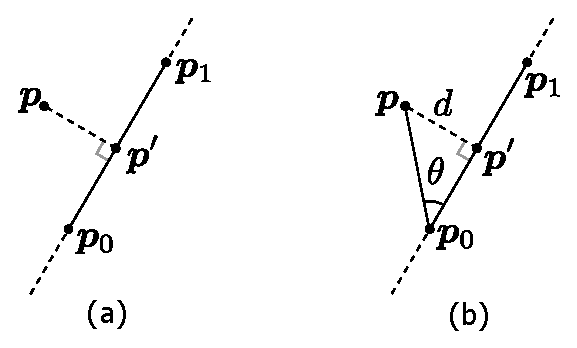
\includegraphics[width=0.4\linewidth]{chap03/Pointlinedistance.eps}
    \caption{(a)给定无限直线和点$\bm p$,则从该点到直线上
        最近点$\bm p'$的向量垂直于该直线。
        (b)因为该向量垂直,我们可以计算从直线上第一点到
        最近点$\bm p'$的距离为$d=\|\bm p-\bm p_0\|\cos\theta$。}
    \label{fig:3.23}
\end{figure}

\refeq{2.1}给出了两向量点积、它们的长度以及夹角余弦的关系。
特别地,它向我们展示了怎样计算从$\bm p_0$到$\bm p$的向量
与从$\bm p_0$到$\bm p_3$的向量之间夹角的余弦:
\begin{align*}
    \cos\theta=\frac{(\bm p-\bm p_0)\cdot(\bm p_3-\bm p_0)}{\|\bm p-\bm p_0\|\|\bm p_3-\bm p_0\|}\, .
\end{align*}

因为从$\bm p'$到$\bm p$的向量垂直于该直线(\reffig{3.23}(b)),
则我们可以计算沿直线从$\bm p_0$到$\bm p'$的距离为
\begin{align*}
    d=\|\bm p-\bm p_0\|\cos\theta=\frac{(\bm p-\bm p_0)\cdot(\bm p_3-\bm p_0)}{\|\bm p_3-\bm p_0\|}\, .
\end{align*}

最后,沿直线的参数偏移量$w$是$d$与直线长度的比值,
\begin{align*}
    w=\frac{d}{\|\bm p_3-\bm p_0\|}=\frac{(\bm p-\bm p_0)\cdot(\bm p_3-\bm p_0)}{\|\bm p_3-\bm p_0\|^2}\, .
\end{align*}

因为事实上相交坐标系统中$\bm p=(0,0)$,所以$w$值的计算最后有所简化。
\begin{lstlisting}
`\initcode{Compute line w that gives minimum distance to sample point}{=}`
`\refvar{Vector2f}{}` segmentDirection = `\refvar{Point2f}{}`(cp[3]) - `\refvar{Point2f}{}`(cp[0]);
`\refvar{Float}{}` denom = segmentDirection.`\refvar{LengthSquared}{}`();
if (denom == 0)
    return false;
`\refvar{Float}{}` w = `\refvar{Dot}{}`(-`\refvar{Vector2f}{}`(cp[0]), segmentDirection) / denom;
\end{lstlisting}

贝塞尔曲线上到候选交点最近(假定)点的参数$u$坐标通过
沿该段$u$的范围线性插值算得。
给定该值,就能计算曲线在该点处的宽度。
\begin{lstlisting}
`\initcode{Compute u coordinate of curve intersection point and hitWidth}{=}`
`\refvar{Float}{}` u = `\refvar{Clamp}{}`(`\refvar{Lerp}{}`(w, u0, u1), u0, u1);
`\refvar{Float}{}` hitWidth = `\refvar{Lerp}{}`(u, `\refvar{common}{}`->`\refvar[CurveCommon::width]{width}{}`[0], `\refvar{common}{}`->`\refvar[CurveCommon::width]{width}{}`[1]);
`\refvar{Normal3f}{}` nHit;
if (`\refvar{common}{}`->`\refvar[CurveCommon::type]{type}{}` == `\refvar{CurveType}{}`::`\refvar{Ribbon}{}`) {
    `\refcode{Scale hitWidth based on ribbon orientation}{}`
}
\end{lstlisting}

对于\refvar{Ribbon}{}曲线,曲线并不总是朝向光线。
相反,它的朝向是在给定于每个端点处的曲面法线之间插值的。
这里,球面线性插值用于插值$u$处的法线(回想\refsub{四元数插值})。
再用规范化的射线方向与丝带朝向间的夹角余弦缩放曲线宽度,
这样它就反映了给定方向的曲线可见宽度。
\begin{lstlisting}
`\initcode{Scale hitWidth based on ribbon orientation}{=}`
`\refvar{Float}{}` sin0 = std::sin((1 - u) * `\refvar{common}{}`->`\refvar{normalAngle}{}`) *
    `\refvar{common}{}`->`\refvar{invSinNormalAngle}{}`;
`\refvar{Float}{}` sin1 = std::sin(u * `\refvar{common}{}`->`\refvar{normalAngle}{}`) *
    `\refvar{common}{}`->`\refvar{invSinNormalAngle}{}`;
nHit = sin0 * `\refvar{common}{}`->`\refvar[CurveCommon::n]{n}{}`[0] + sin1 * `\refvar{common}{}`->`\refvar[CurveCommon::n]{n}{}`[1];
hitWidth *= `\refvar{AbsDot}{}`(nHit, ray.`\refvar[Ray::d]{d}{}`) / rayLength;
\end{lstlisting}

为了最终将可能的相交处分类为命中或未命中,
必须用函数\refvar{EvalBezier}{()}
求贝塞尔曲线在$u$处的值
(因为控制点{\ttfamily cp}表示当前考虑的曲线段,
然而既然$w$在范围$[0,1]$内,在函数调用中使用$w$而不是$u$就很重要)。
曲线在该点的导数很快也会有用,所以现在记录下来。

我们想测试从$\bm p$到曲线上该点{\ttfamily pc}的
距离是否小于曲线宽度的一半。
因为$\bm p=(0,0)$,我们可以等价地测试从{\ttfamily pc}到原点
的距离是否小于宽度的一半,或者等价地,
平方距离是否小于宽度平方的四分之一。
如果该测试通过,最后一件事是检查交点是否在射线的参数$t$范围内。
\begin{lstlisting}
`\initcode{Test intersection point against curve width}{=}`
`\refvar{Vector3f}{}` dpcdw;
`\refvar{Point3f}{}` pc = `\refvar{EvalBezier}{}`(cp, `\refvar{Clamp}{}`(w, 0, 1), &dpcdw);
`\refvar{Float}{}` ptCurveDist2 = pc.x * pc.x + pc.y * pc.y;
if (ptCurveDist2 > hitWidth * hitWidth * .25)
    return false;
if (pc.z < 0 || pc.z > zMax)
    return false;
\end{lstlisting}

\refvar{EvalBezier}{()}计算簇$\bm p(u,u,u)$来求贝塞尔样条上的一点。
它也可选地返回曲线在该点处的导数\sidenote{译者注:读者可以动手验算一下。}。
\begin{lstlisting}
`\refcode{Curve Utility Functions}{+=}\lastcode{CurveUtilityFunctions}`
static `\refvar{Point3f}{}` `\initvar{EvalBezier}{}`(const `\refvar{Point3f}{}` cp[4], `\refvar{Float}{}` u,
        `\refvar{Vector3f}{}` *deriv = nullptr) {
    `\refvar{Point3f}{}` cp1[3] = { `\refvar{Lerp}{}`(u, cp[0], cp[1]), `\refvar{Lerp}{}`(u, cp[1], cp[2]),
                       `\refvar{Lerp}{}`(u, cp[2], cp[3]) };
    `\refvar{Point3f}{}` cp2[2] = { `\refvar{Lerp}{}`(u, cp1[0], cp1[1]), `\refvar{Lerp}{}`(u, cp1[1], cp1[2]) };
    if (deriv)
        *deriv = (`\refvar{Float}{}`)3 * (cp2[1] - cp2[0]);
    return `\refvar{Lerp}{}`(u, cp2[0], cp2[1]);
}
\end{lstlisting}

如果之前的测试都通过了,我们就找到了有效的相交,
现在可以计算交点的$v$坐标了。
曲线的$v$坐标在0到1内变化,曲线中心取值为0.5;
这里我们根据过曲线上的点{\ttfamily pc}和沿其导数的点的边函数
将交点$(0,0)$分类,决定交点在中心的哪边以及该怎样计算$v$。
\begin{lstlisting}
`\initcode{Compute v coordinate of curve intersection point}{=}`
`\refvar{Float}{}` ptCurveDist = std::sqrt(ptCurveDist2);
`\refvar{Float}{}` edgeFunc = dpcdw.x * -pc.y + pc.x * dpcdw.y;
`\refvar{Float}{}` v = (edgeFunc > 0) ? 0.5f + ptCurveDist / hitWidth :
                           0.5f - ptCurveDist / hitWidth;
\end{lstlisting}

最后,计算偏导数,相交处的\refvar{SurfaceInteraction}{}可以初始化了。
\begin{lstlisting}
`\initcode{Compute hit t and partial derivatives for curve intersection}{=}`
if (tHit != nullptr) {
    *tHit = pc.z / rayLength;
    `\refcode{Compute error bounds for curve intersection}{}`
    `\refcode{Compute $\partial$p/$\partial$u and $\partial$p/$\partial$v for curve intersection}{}`
    *isect = (*`\refvar{ObjectToWorld}{}`)(`\refvar{SurfaceInteraction}{}`(
        ray(pc.z), pError, `\refvar{Point2f}{}`(u, v), -ray.`\refvar[Ray::d]{d}{}`, dpdu, dpdv,
        `\refvar{Normal3f}{}`(0, 0, 0), `\refvar{Normal3f}{}`(0, 0, 0), ray.`\refvar[Ray::time]{time}{}`, this));
}
\end{lstlisting}

偏导数$\displaystyle\frac{\partial \bm p}{\partial u}$直接
来自于底层贝塞尔曲线的导数。
第二个偏导数$\displaystyle\frac{\partial \bm p}{\partial v}$则
基于曲线类型用不同方式计算。
对于丝带,我们有$\displaystyle\frac{\partial \bm p}{\partial u}$和
曲面法线,因此$\displaystyle\frac{\partial \bm p}{\partial v}$必须
是使得$\displaystyle\frac{\partial \bm p}{\partial u}\times\frac{\partial \bm p}{\partial v}=\bm n$的向量
且长度等于曲线宽度。
\begin{lstlisting}
`\initcode{Compute $\partial$p/$\partial$u and $\partial$p/$\partial$v for curve intersection}{=}`
`\refvar{Vector3f}{}` dpdu, dpdv;
`\refvar{EvalBezier}{}`(`\refvar{common}{}`->`\refvar{cpObj}{}`, u, &dpdu);
if (`\refvar{common}{}`->`\refvar[CurveCommon::type]{type}{}` == `\refvar{CurveType}{}`::`\refvar{Ribbon}{}`)
    dpdv = `\refvar{Normalize}{}`(`\refvar{Cross}{}`(nHit, dpdu)) * hitWidth;
else {
    `\refcode{Compute curve $\partial$p/$\partial$v for flat and cylinder curves}{}`
}
\end{lstlisting}

对于平坦和圆柱曲线,我们变换$\displaystyle\frac{\partial \bm p}{\partial u}$到相交坐标系统。
对于平坦曲线,我们知道$\displaystyle\frac{\partial \bm p}{\partial v}$位于$xy$平面内、
垂直于$\displaystyle\frac{\partial \bm p}{\partial u}$且长度等于{\ttfamily hitWidth}。
我们可以用和之前求垂直于曲线段的边界边同样的方法求得2D垂直向量。
\begin{lstlisting}
`\initcode{Compute curve $\partial$p/$\partial$v for flat and cylinder curves}{=}`
`\refvar{Vector3f}{}` dpduPlane = (`\refvar[Transform::Inverse]{Inverse}{}`(rayToObject))(dpdu);
`\refvar{Vector3f}{}` dpdvPlane = `\refvar{Normalize}{}`(`\refvar{Vector3f}{}`(-dpduPlane.y, dpduPlane.x, 0)) *
                     hitWidth;
if (`\refvar{common}{}`->`\refvar[CurveCommon::type]{type}{}` == `\refvar{CurveType}{}`::`\refvar[CurveType::Cylinder]{Cylinder}{}`) {
    `\refcode{Rotate dpdvPlane to give cylindrical appearance}{}`
}
dpdv = rayToObject(dpdvPlane);
\end{lstlisting}

圆柱曲线的向量$\displaystyle\frac{\partial \bm p}{\partial v}$沿轴{\ttfamily dpduPlane}旋转
使其外观像圆柱体横截面。
\begin{lstlisting}
`\initcode{Rotate dpdvPlane to give cylindrical appearance}{=}`
`\refvar{Float}{}` theta = `\refvar{Lerp}{}`(v, -90., 90.);
`\refvar{Transform}{}` rot = `\refvar{Rotate}{}`(-theta, dpduPlane);
dpdvPlane = rot(dpdvPlane);
\end{lstlisting}

这里没有介绍的方法\refvar{Curve::Area}{()}首先
用其控制点连线长度近似曲线长度。
然后它再用该长度乘以其范围内宽度的均值以近似整个曲面面积。

\section{细分曲面}\label{sec:细分曲面}
\begin{remark}
    本节含有高级内容,第一次阅读时可以跳过。
\end{remark}

本章我们要定义的最后一个形状表示
实现了\keyindex{细分曲面}{subdivision surface}{surface曲面},
该表示尤其适合描述复杂光滑形状。
特定网格的细分曲面定义为将网格面反复细分为更小面
然后用旧顶点位置的加权组合求新顶点位置。

对于适当选择的细分规则,当细分步数趋于无穷时,
该过程会收敛到给出一个光滑的\keyindex{极限曲面}{limit surface}{surface曲面}。
实践中,只需少量级别的细分通常就足以得到极限曲面的良好近似。
\reffig{3.24}展示了一个细分的简单例子,
其中四面体被细分了零次、一次、两次和六次。
\begin{figure}[htbp]
    \centering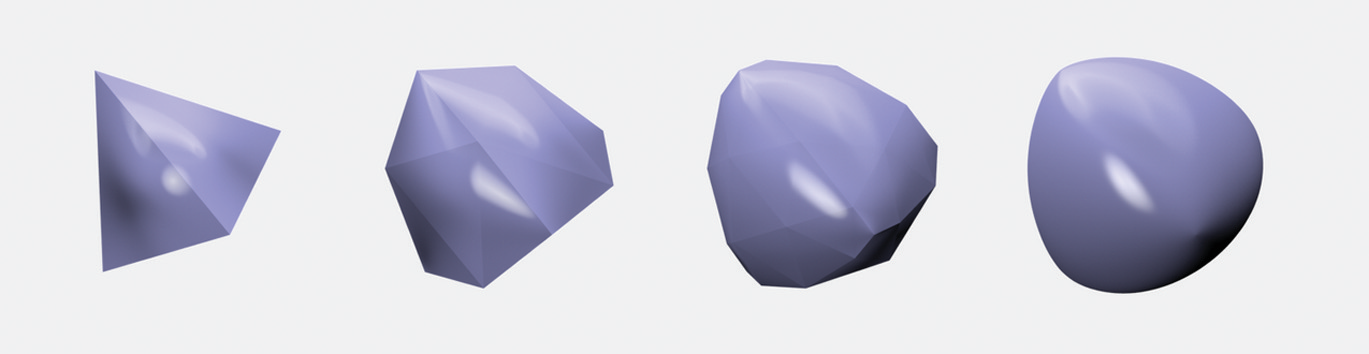
\includegraphics[width=\linewidth]{chap03/tetsubdiv.png}
    \caption{四面体的细分。从左到右使用了零步、一步、两步和六步细分
        (在零级时,顶点只是移动到极限曲面上)。
        随着细分得越来越多,网格逼近极限曲面,即原始网格描述的光滑曲面。
        随着执行更多级别的细分,注意高光如何变得更加准确、轮廓边缘如何变得更加平滑。}
    \label{fig:3.24}
\end{figure}

\reffig{3.25}展示了对Killeroo\sidenote{译者注:猜测此名字与一澳大利亚漫画中的袋鼠角色名有关。}模型应用细分的效果;
上面是原始控制网格,下面是控制网格表示的细分曲面。
\begin{figure}[htbp]
    \centering
    \subfloat[控制网格]{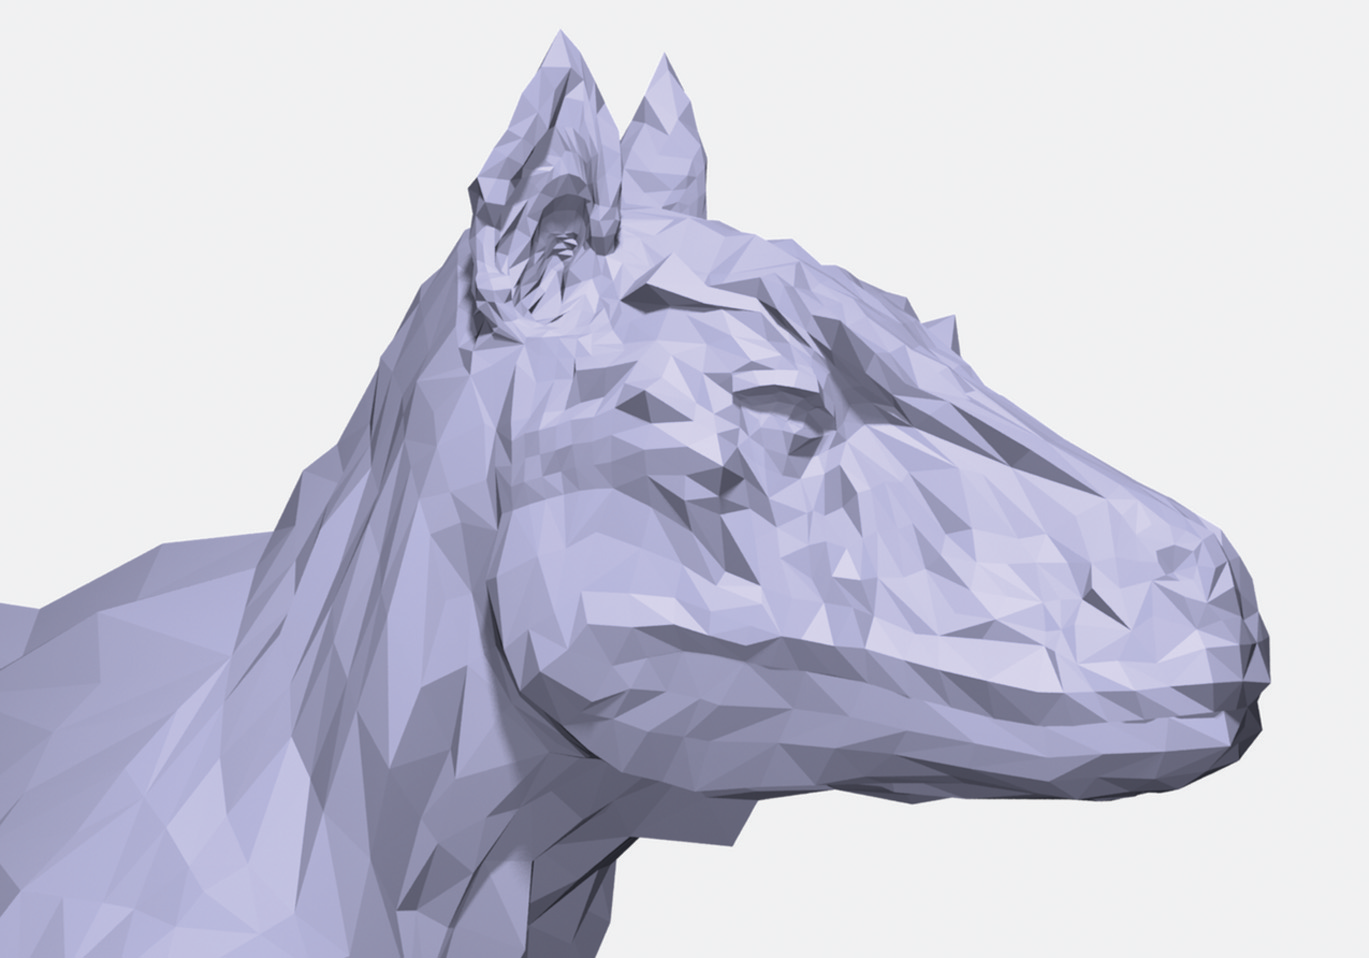
\includegraphics[width=\linewidth]{chap03/killeroo-control.png}\label{fig:3.25.1}}\\
    \subfloat[细分网格]{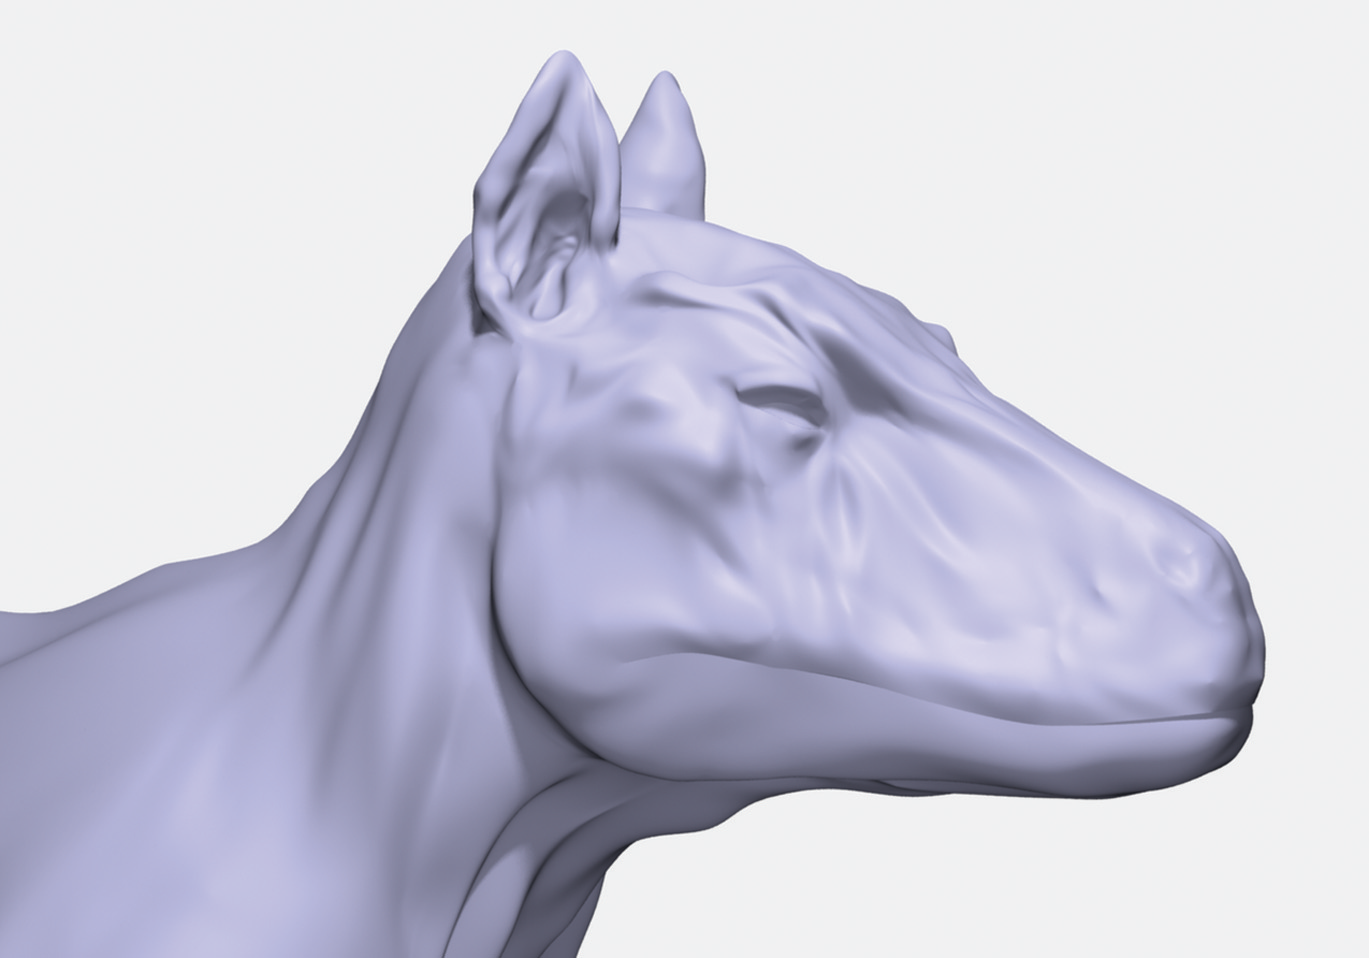
\includegraphics[width=\linewidth]{chap03/killeroo-subdivided.png}\label{fig:3.25.2}}
    \caption{对Killeroo模型应用细分。(1)控制网格描述了(2)结果细分曲面。
        细分非常适合建模这样的形状,因为它能通过细化控制网格轻松添加局部细节,
        对最终曲面没有拓扑结构限制。(模型由headus/Rezard提供。)}
    \label{fig:3.25}
\end{figure}


因为在曲面的多边形和基于样条的表示方面有一些重要优势,
细分曲面近年来得到广泛运用,尽管它在20世纪70年代就被发明了。
细分的优势包括:
\begin{itemize}
    \item 细分曲面是平滑的,而多边形网格与之相反,无论建模得多细致,靠近观察会有小面。
    \item 建模系统中现有的多数基本结构可以重定向到细分。
          建模多边形网格的经典技术工具箱可以应用到建模细分控制网格上。
    \item 细分曲面非常适合描述有复杂拓扑结构的物体,
          因为它们以任意(\keyindex{流形}{manifold}{})拓扑结构的控制网格为起点。
          参数化曲面模型一般不能很好地处理复杂拓扑结构。
    \item 细分方法常常是基于样条的曲面表示的推广,
          所以样条曲面常常可以由通用细分曲面渲染器运行。
    \item 通过简单地对控制网格的适当部分添加面,它能轻松对细分曲面局部区域添加细节。
          用样条表示则要困难得多。
\end{itemize}
\begin{figure}[htbp]
    \centering%LaTeX with PSTricks extensions
%%Creator: Inkscape 1.0.1 (3bc2e813f5, 2020-09-07)
%%Please note this file requires PSTricks extensions
\psset{xunit=.5pt,yunit=.5pt,runit=.5pt}
\begin{pspicture}(487.94000244,169.97000122)
{
\newrgbcolor{curcolor}{0.7019608 0.7019608 0.7019608}
\pscustom[linestyle=none,fillstyle=solid,fillcolor=curcolor]
{
\newpath
\moveto(96.28,168.97000122)
\lineto(143.98,86.34000122)
\lineto(191.69,3.72000122)
\lineto(96.28,3.72000122)
\lineto(0.87,3.72000122)
\lineto(48.57,86.34000122)
\closepath
}
}
{
\newrgbcolor{curcolor}{0 0 0}
\pscustom[linewidth=1,linecolor=curcolor]
{
\newpath
\moveto(96.28,168.97000122)
\lineto(143.98,86.34000122)
\lineto(191.69,3.72000122)
\lineto(96.28,3.72000122)
\lineto(0.87,3.72000122)
\lineto(48.57,86.34000122)
\closepath
}
}
{
\newrgbcolor{curcolor}{0.7019608 0.7019608 0.7019608}
\pscustom[linestyle=none,fillstyle=solid,fillcolor=curcolor]
{
\newpath
\moveto(96.28,4.73000122)
\lineto(72.9,45.22000122)
\lineto(49.52,85.71000122)
\lineto(96.28,85.71000122)
\lineto(143.03,85.71000122)
\lineto(119.65,45.22000122)
\closepath
}
}
{
\newrgbcolor{curcolor}{0 0 0}
\pscustom[linewidth=0.5,linecolor=curcolor]
{
\newpath
\moveto(96.28,4.73000122)
\lineto(72.9,45.22000122)
\lineto(49.52,85.71000122)
\lineto(96.28,85.71000122)
\lineto(143.03,85.71000122)
\lineto(119.65,45.22000122)
\closepath
}
}
{
\newrgbcolor{curcolor}{0.7019608 0.7019608 0.7019608}
\pscustom[linestyle=none,fillstyle=solid,fillcolor=curcolor]
{
\newpath
\moveto(391.67,168.97000122)
\lineto(439.37,86.34000122)
\lineto(487.08,3.72000122)
\lineto(391.67,3.72000122)
\lineto(296.26,3.72000122)
\lineto(343.96,86.34000122)
\closepath
}
}
{
\newrgbcolor{curcolor}{0 0 0}
\pscustom[linewidth=1,linecolor=curcolor]
{
\newpath
\moveto(391.67,168.97000122)
\lineto(439.37,86.34000122)
\lineto(487.08,3.72000122)
\lineto(391.67,3.72000122)
\lineto(296.26,3.72000122)
\lineto(343.96,86.34000122)
\closepath
}
}
{
\newrgbcolor{curcolor}{0.7019608 0.7019608 0.7019608}
\pscustom[linestyle=none,fillstyle=solid,fillcolor=curcolor]
{
\newpath
\moveto(391.67,4.73000122)
\lineto(368.29,45.22000122)
\lineto(344.92,85.71000122)
\lineto(391.67,85.71000122)
\lineto(438.42,85.71000122)
\lineto(415.04,45.22000122)
\closepath
}
}
{
\newrgbcolor{curcolor}{0 0 0}
\pscustom[linewidth=0.5,linecolor=curcolor]
{
\newpath
\moveto(391.67,4.73000122)
\lineto(368.29,45.22000122)
\lineto(344.92,85.71000122)
\lineto(391.67,85.71000122)
\lineto(438.42,85.71000122)
\lineto(415.04,45.22000122)
\closepath
}
}
{
\newrgbcolor{curcolor}{0.7019608 0.7019608 0.7019608}
\pscustom[linestyle=none,fillstyle=solid,fillcolor=curcolor]
{
\newpath
\moveto(391.89,86.41000122)
\lineto(380.43,106.25000122)
\lineto(368.98,126.09000122)
\lineto(391.89,126.09000122)
\lineto(414.8,126.09000122)
\lineto(403.34,106.25000122)
\closepath
}
}
{
\newrgbcolor{curcolor}{0 0 0}
\pscustom[linewidth=0.5,linecolor=curcolor,linestyle=dashed,dash=2]
{
\newpath
\moveto(391.89,86.41000122)
\lineto(380.43,106.25000122)
\lineto(368.98,126.09000122)
\lineto(391.89,126.09000122)
\lineto(414.8,126.09000122)
\lineto(403.34,106.25000122)
\closepath
}
}
{
\newrgbcolor{curcolor}{0.7019608 0.7019608 0.7019608}
\pscustom[linestyle=none,fillstyle=solid,fillcolor=curcolor]
{
\newpath
\moveto(344.09,4.78000122)
\lineto(332.64,24.62000122)
\lineto(321.19,44.46000122)
\lineto(344.09,44.46000122)
\lineto(367,44.46000122)
\lineto(355.55,24.62000122)
\closepath
}
}
{
\newrgbcolor{curcolor}{0 0 0}
\pscustom[linewidth=0.5,linecolor=curcolor,linestyle=dashed,dash=2]
{
\newpath
\moveto(344.09,4.78000122)
\lineto(332.64,24.62000122)
\lineto(321.19,44.46000122)
\lineto(344.09,44.46000122)
\lineto(367,44.46000122)
\lineto(355.55,24.62000122)
\closepath
}
}
{
\newrgbcolor{curcolor}{0.7019608 0.7019608 0.7019608}
\pscustom[linestyle=none,fillstyle=solid,fillcolor=curcolor]
{
\newpath
\moveto(439.39,5.37000122)
\lineto(427.94,25.21000122)
\lineto(416.48,45.05000122)
\lineto(439.39,45.05000122)
\lineto(462.3,45.05000122)
\lineto(450.84,25.21000122)
\closepath
}
}
{
\newrgbcolor{curcolor}{0 0 0}
\pscustom[linewidth=0.5,linecolor=curcolor,linestyle=dashed,dash=2]
{
\newpath
\moveto(439.39,5.37000122)
\lineto(427.94,25.21000122)
\lineto(416.48,45.05000122)
\lineto(439.39,45.05000122)
\lineto(462.3,45.05000122)
\lineto(450.84,25.21000122)
\closepath
}
}
{
\newrgbcolor{curcolor}{0.7019608 0.7019608 0.7019608}
\pscustom[linestyle=none,fillstyle=solid,fillcolor=curcolor]
{
\newpath
\moveto(392.26,85.27000122)
\lineto(403.71,65.43000122)
\lineto(415.16,45.59000122)
\lineto(392.26,45.59000122)
\lineto(369.35,45.59000122)
\lineto(380.8,65.43000122)
\closepath
}
}
{
\newrgbcolor{curcolor}{0 0 0}
\pscustom[linewidth=0.5,linecolor=curcolor,linestyle=dashed,dash=2]
{
\newpath
\moveto(392.26,85.27000122)
\lineto(403.71,65.43000122)
\lineto(415.16,45.59000122)
\lineto(392.26,45.59000122)
\lineto(369.35,45.59000122)
\lineto(380.8,65.43000122)
\closepath
}
}
{
\newrgbcolor{curcolor}{0 0 0}
\pscustom[linestyle=none,fillstyle=solid,fillcolor=curcolor]
{
\newpath
\moveto(419.14999509,126.22999954)
\curveto(419.14999509,129.37511236)(415.34769602,130.94962069)(413.124035,128.72595966)
\curveto(410.90037397,126.50229864)(412.4748823,122.69999957)(415.61999512,122.69999957)
\curveto(418.76510794,122.69999957)(420.33961626,126.50229864)(418.11595524,128.72595966)
\curveto(415.89229421,130.94962069)(412.08999515,129.37511236)(412.08999515,126.22999954)
\curveto(412.08999515,123.08488672)(415.89229421,121.5103784)(418.11595524,123.73403942)
\curveto(420.33961626,125.95770045)(418.76510794,129.75999951)(415.61999512,129.75999951)
\curveto(412.4748823,129.75999951)(410.90037397,125.95770045)(413.124035,123.73403942)
\curveto(415.34769602,121.5103784)(419.14999509,123.08488672)(419.14999509,126.22999954)
\closepath
}
}
{
\newrgbcolor{curcolor}{0 0 0}
\pscustom[linewidth=1,linecolor=curcolor]
{
\newpath
\moveto(419.14999509,126.22999954)
\curveto(419.14999509,129.37511236)(415.34769602,130.94962069)(413.124035,128.72595966)
\curveto(410.90037397,126.50229864)(412.4748823,122.69999957)(415.61999512,122.69999957)
\curveto(418.76510794,122.69999957)(420.33961626,126.50229864)(418.11595524,128.72595966)
\curveto(415.89229421,130.94962069)(412.08999515,129.37511236)(412.08999515,126.22999954)
\curveto(412.08999515,123.08488672)(415.89229421,121.5103784)(418.11595524,123.73403942)
\curveto(420.33961626,125.95770045)(418.76510794,129.75999951)(415.61999512,129.75999951)
\curveto(412.4748823,129.75999951)(410.90037397,125.95770045)(413.124035,123.73403942)
\curveto(415.34769602,121.5103784)(419.14999509,123.08488672)(419.14999509,126.22999954)
\closepath
}
}
{
\newrgbcolor{curcolor}{0 0 0}
\pscustom[linestyle=none,fillstyle=solid,fillcolor=curcolor]
{
\newpath
\moveto(395.51001096,85.79000092)
\curveto(395.51001096,88.93511374)(391.70771189,90.50962206)(389.48405087,88.28596104)
\curveto(387.26038984,86.06230001)(388.83489817,82.26000094)(391.98001099,82.26000094)
\curveto(395.12512381,82.26000094)(396.69963213,86.06230001)(394.47597111,88.28596104)
\curveto(392.25231008,90.50962206)(388.45001101,88.93511374)(388.45001101,85.79000092)
\curveto(388.45001101,82.6448881)(392.25231008,81.07037977)(394.47597111,83.2940408)
\curveto(396.69963213,85.51770182)(395.12512381,89.32000089)(391.98001099,89.32000089)
\curveto(388.83489817,89.32000089)(387.26038984,85.51770182)(389.48405087,83.2940408)
\curveto(391.70771189,81.07037977)(395.51001096,82.6448881)(395.51001096,85.79000092)
\closepath
}
}
{
\newrgbcolor{curcolor}{0 0 0}
\pscustom[linewidth=1,linecolor=curcolor]
{
\newpath
\moveto(395.51001096,85.79000092)
\curveto(395.51001096,88.93511374)(391.70771189,90.50962206)(389.48405087,88.28596104)
\curveto(387.26038984,86.06230001)(388.83489817,82.26000094)(391.98001099,82.26000094)
\curveto(395.12512381,82.26000094)(396.69963213,86.06230001)(394.47597111,88.28596104)
\curveto(392.25231008,90.50962206)(388.45001101,88.93511374)(388.45001101,85.79000092)
\curveto(388.45001101,82.6448881)(392.25231008,81.07037977)(394.47597111,83.2940408)
\curveto(396.69963213,85.51770182)(395.12512381,89.32000089)(391.98001099,89.32000089)
\curveto(388.83489817,89.32000089)(387.26038984,85.51770182)(389.48405087,83.2940408)
\curveto(391.70771189,81.07037977)(395.51001096,82.6448881)(395.51001096,85.79000092)
\closepath
}
}
{
\newrgbcolor{curcolor}{0 0 0}
\pscustom[linestyle=none,fillstyle=solid,fillcolor=curcolor]
{
\newpath
\moveto(370.98999143,127.18000031)
\curveto(370.98999143,130.32511313)(367.18769236,131.89962145)(364.96403134,129.67596042)
\curveto(362.74037031,127.4522994)(364.31487864,123.65000033)(367.45999146,123.65000033)
\curveto(370.60510428,123.65000033)(372.1796126,127.4522994)(369.95595157,129.67596042)
\curveto(367.73229055,131.89962145)(363.92999148,130.32511313)(363.92999148,127.18000031)
\curveto(363.92999148,124.03488749)(367.73229055,122.46037916)(369.95595157,124.68404019)
\curveto(372.1796126,126.90770121)(370.60510428,130.71000028)(367.45999146,130.71000028)
\curveto(364.31487864,130.71000028)(362.74037031,126.90770121)(364.96403134,124.68404019)
\curveto(367.18769236,122.46037916)(370.98999143,124.03488749)(370.98999143,127.18000031)
\closepath
}
}
{
\newrgbcolor{curcolor}{0 0 0}
\pscustom[linewidth=1,linecolor=curcolor]
{
\newpath
\moveto(370.98999143,127.18000031)
\curveto(370.98999143,130.32511313)(367.18769236,131.89962145)(364.96403134,129.67596042)
\curveto(362.74037031,127.4522994)(364.31487864,123.65000033)(367.45999146,123.65000033)
\curveto(370.60510428,123.65000033)(372.1796126,127.4522994)(369.95595157,129.67596042)
\curveto(367.73229055,131.89962145)(363.92999148,130.32511313)(363.92999148,127.18000031)
\curveto(363.92999148,124.03488749)(367.73229055,122.46037916)(369.95595157,124.68404019)
\curveto(372.1796126,126.90770121)(370.60510428,130.71000028)(367.45999146,130.71000028)
\curveto(364.31487864,130.71000028)(362.74037031,126.90770121)(364.96403134,124.68404019)
\curveto(367.18769236,122.46037916)(370.98999143,124.03488749)(370.98999143,127.18000031)
\closepath
}
}
{
\newrgbcolor{curcolor}{0 0 0}
\pscustom[linestyle=none,fillstyle=solid,fillcolor=curcolor]
{
\newpath
\moveto(418.45999265,46.02999878)
\curveto(418.45999265,49.1751116)(414.65769358,50.74961993)(412.43403256,48.5259589)
\curveto(410.21037153,46.30229787)(411.78487986,42.49999881)(414.92999268,42.49999881)
\curveto(418.0751055,42.49999881)(419.64961382,46.30229787)(417.4259528,48.5259589)
\curveto(415.20229177,50.74961993)(411.3999927,49.1751116)(411.3999927,46.02999878)
\curveto(411.3999927,42.88488596)(415.20229177,41.31037763)(417.4259528,43.53403866)
\curveto(419.64961382,45.75769969)(418.0751055,49.55999875)(414.92999268,49.55999875)
\curveto(411.78487986,49.55999875)(410.21037153,45.75769969)(412.43403256,43.53403866)
\curveto(414.65769358,41.31037763)(418.45999265,42.88488596)(418.45999265,46.02999878)
\closepath
}
}
{
\newrgbcolor{curcolor}{0 0 0}
\pscustom[linewidth=1,linecolor=curcolor]
{
\newpath
\moveto(418.45999265,46.02999878)
\curveto(418.45999265,49.1751116)(414.65769358,50.74961993)(412.43403256,48.5259589)
\curveto(410.21037153,46.30229787)(411.78487986,42.49999881)(414.92999268,42.49999881)
\curveto(418.0751055,42.49999881)(419.64961382,46.30229787)(417.4259528,48.5259589)
\curveto(415.20229177,50.74961993)(411.3999927,49.1751116)(411.3999927,46.02999878)
\curveto(411.3999927,42.88488596)(415.20229177,41.31037763)(417.4259528,43.53403866)
\curveto(419.64961382,45.75769969)(418.0751055,49.55999875)(414.92999268,49.55999875)
\curveto(411.78487986,49.55999875)(410.21037153,45.75769969)(412.43403256,43.53403866)
\curveto(414.65769358,41.31037763)(418.45999265,42.88488596)(418.45999265,46.02999878)
\closepath
}
}
{
\newrgbcolor{curcolor}{0 0 0}
\pscustom[linestyle=none,fillstyle=solid,fillcolor=curcolor]
{
\newpath
\moveto(371.64999509,45.45000458)
\curveto(371.64999509,48.5951174)(367.84769602,50.16962572)(365.624035,47.9459647)
\curveto(363.40037397,45.72230367)(364.9748823,41.92000461)(368.11999512,41.92000461)
\curveto(371.26510794,41.92000461)(372.83961626,45.72230367)(370.61595524,47.9459647)
\curveto(368.39229421,50.16962572)(364.58999515,48.5951174)(364.58999515,45.45000458)
\curveto(364.58999515,42.30489176)(368.39229421,40.73038343)(370.61595524,42.95404446)
\curveto(372.83961626,45.17770548)(371.26510794,48.98000455)(368.11999512,48.98000455)
\curveto(364.9748823,48.98000455)(363.40037397,45.17770548)(365.624035,42.95404446)
\curveto(367.84769602,40.73038343)(371.64999509,42.30489176)(371.64999509,45.45000458)
\closepath
}
}
{
\newrgbcolor{curcolor}{0 0 0}
\pscustom[linewidth=1,linecolor=curcolor]
{
\newpath
\moveto(371.64999509,45.45000458)
\curveto(371.64999509,48.5951174)(367.84769602,50.16962572)(365.624035,47.9459647)
\curveto(363.40037397,45.72230367)(364.9748823,41.92000461)(368.11999512,41.92000461)
\curveto(371.26510794,41.92000461)(372.83961626,45.72230367)(370.61595524,47.9459647)
\curveto(368.39229421,50.16962572)(364.58999515,48.5951174)(364.58999515,45.45000458)
\curveto(364.58999515,42.30489176)(368.39229421,40.73038343)(370.61595524,42.95404446)
\curveto(372.83961626,45.17770548)(371.26510794,48.98000455)(368.11999512,48.98000455)
\curveto(364.9748823,48.98000455)(363.40037397,45.17770548)(365.624035,42.95404446)
\curveto(367.84769602,40.73038343)(371.64999509,42.30489176)(371.64999509,45.45000458)
\closepath
}
}
{
\newrgbcolor{curcolor}{0 0 0}
\pscustom[linestyle=none,fillstyle=solid,fillcolor=curcolor]
{
\newpath
\moveto(466.45999265,45.13999939)
\curveto(466.45999265,48.28511221)(462.65769358,49.85962054)(460.43403256,47.63595951)
\curveto(458.21037153,45.41229848)(459.78487986,41.60999942)(462.92999268,41.60999942)
\curveto(466.0751055,41.60999942)(467.64961382,45.41229848)(465.4259528,47.63595951)
\curveto(463.20229177,49.85962054)(459.3999927,48.28511221)(459.3999927,45.13999939)
\curveto(459.3999927,41.99488657)(463.20229177,40.42037824)(465.4259528,42.64403927)
\curveto(467.64961382,44.8677003)(466.0751055,48.66999936)(462.92999268,48.66999936)
\curveto(459.78487986,48.66999936)(458.21037153,44.8677003)(460.43403256,42.64403927)
\curveto(462.65769358,40.42037824)(466.45999265,41.99488657)(466.45999265,45.13999939)
\closepath
}
}
{
\newrgbcolor{curcolor}{0 0 0}
\pscustom[linewidth=1,linecolor=curcolor]
{
\newpath
\moveto(466.45999265,45.13999939)
\curveto(466.45999265,48.28511221)(462.65769358,49.85962054)(460.43403256,47.63595951)
\curveto(458.21037153,45.41229848)(459.78487986,41.60999942)(462.92999268,41.60999942)
\curveto(466.0751055,41.60999942)(467.64961382,45.41229848)(465.4259528,47.63595951)
\curveto(463.20229177,49.85962054)(459.3999927,48.28511221)(459.3999927,45.13999939)
\curveto(459.3999927,41.99488657)(463.20229177,40.42037824)(465.4259528,42.64403927)
\curveto(467.64961382,44.8677003)(466.0751055,48.66999936)(462.92999268,48.66999936)
\curveto(459.78487986,48.66999936)(458.21037153,44.8677003)(460.43403256,42.64403927)
\curveto(462.65769358,40.42037824)(466.45999265,41.99488657)(466.45999265,45.13999939)
\closepath
}
}
{
\newrgbcolor{curcolor}{0 0 0}
\pscustom[linestyle=none,fillstyle=solid,fillcolor=curcolor]
{
\newpath
\moveto(323.7000134,45.41999817)
\curveto(323.7000134,48.56511099)(319.89771433,50.13961932)(317.67405331,47.91595829)
\curveto(315.45039228,45.69229726)(317.02490061,41.8899982)(320.17001343,41.8899982)
\curveto(323.31512625,41.8899982)(324.88963457,45.69229726)(322.66597355,47.91595829)
\curveto(320.44231252,50.13961932)(316.64001346,48.56511099)(316.64001346,45.41999817)
\curveto(316.64001346,42.27488535)(320.44231252,40.70037702)(322.66597355,42.92403805)
\curveto(324.88963457,45.14769908)(323.31512625,48.94999814)(320.17001343,48.94999814)
\curveto(317.02490061,48.94999814)(315.45039228,45.14769908)(317.67405331,42.92403805)
\curveto(319.89771433,40.70037702)(323.7000134,42.27488535)(323.7000134,45.41999817)
\closepath
}
}
{
\newrgbcolor{curcolor}{0 0 0}
\pscustom[linewidth=1,linecolor=curcolor]
{
\newpath
\moveto(323.7000134,45.41999817)
\curveto(323.7000134,48.56511099)(319.89771433,50.13961932)(317.67405331,47.91595829)
\curveto(315.45039228,45.69229726)(317.02490061,41.8899982)(320.17001343,41.8899982)
\curveto(323.31512625,41.8899982)(324.88963457,45.69229726)(322.66597355,47.91595829)
\curveto(320.44231252,50.13961932)(316.64001346,48.56511099)(316.64001346,45.41999817)
\curveto(316.64001346,42.27488535)(320.44231252,40.70037702)(322.66597355,42.92403805)
\curveto(324.88963457,45.14769908)(323.31512625,48.94999814)(320.17001343,48.94999814)
\curveto(317.02490061,48.94999814)(315.45039228,45.14769908)(317.67405331,42.92403805)
\curveto(319.89771433,40.70037702)(323.7000134,42.27488535)(323.7000134,45.41999817)
\closepath
}
}
{
\newrgbcolor{curcolor}{0 0 0}
\pscustom[linestyle=none,fillstyle=solid,fillcolor=curcolor]
{
\newpath
\moveto(347.83999753,4.04000854)
\curveto(347.83999753,7.18512136)(344.03769847,8.75962969)(341.81403744,6.53596866)
\curveto(339.59037641,4.31230764)(341.16488474,0.51000857)(344.30999756,0.51000857)
\curveto(347.45511038,0.51000857)(349.0296187,4.31230764)(346.80595768,6.53596866)
\curveto(344.58229665,8.75962969)(340.77999759,7.18512136)(340.77999759,4.04000854)
\curveto(340.77999759,0.89489572)(344.58229665,-0.6796126)(346.80595768,1.54404843)
\curveto(349.0296187,3.76770945)(347.45511038,7.57000852)(344.30999756,7.57000852)
\curveto(341.16488474,7.57000852)(339.59037641,3.76770945)(341.81403744,1.54404843)
\curveto(344.03769847,-0.6796126)(347.83999753,0.89489572)(347.83999753,4.04000854)
\closepath
}
}
{
\newrgbcolor{curcolor}{0 0 0}
\pscustom[linewidth=1,linecolor=curcolor]
{
\newpath
\moveto(347.83999753,4.04000854)
\curveto(347.83999753,7.18512136)(344.03769847,8.75962969)(341.81403744,6.53596866)
\curveto(339.59037641,4.31230764)(341.16488474,0.51000857)(344.30999756,0.51000857)
\curveto(347.45511038,0.51000857)(349.0296187,4.31230764)(346.80595768,6.53596866)
\curveto(344.58229665,8.75962969)(340.77999759,7.18512136)(340.77999759,4.04000854)
\curveto(340.77999759,0.89489572)(344.58229665,-0.6796126)(346.80595768,1.54404843)
\curveto(349.0296187,3.76770945)(347.45511038,7.57000852)(344.30999756,7.57000852)
\curveto(341.16488474,7.57000852)(339.59037641,3.76770945)(341.81403744,1.54404843)
\curveto(344.03769847,-0.6796126)(347.83999753,0.89489572)(347.83999753,4.04000854)
\closepath
}
}
{
\newrgbcolor{curcolor}{0 0 0}
\pscustom[linestyle=none,fillstyle=solid,fillcolor=curcolor]
{
\newpath
\moveto(443.57000852,4.02999878)
\curveto(443.57000852,7.1751116)(439.76770945,8.74961993)(437.54404843,6.5259589)
\curveto(435.3203874,4.30229787)(436.89489572,0.49999881)(440.04000854,0.49999881)
\curveto(443.18512136,0.49999881)(444.75962969,4.30229787)(442.53596866,6.5259589)
\curveto(440.31230764,8.74961993)(436.51000857,7.1751116)(436.51000857,4.02999878)
\curveto(436.51000857,0.88488596)(440.31230764,-0.68962237)(442.53596866,1.53403866)
\curveto(444.75962969,3.75769969)(443.18512136,7.55999875)(440.04000854,7.55999875)
\curveto(436.89489572,7.55999875)(435.3203874,3.75769969)(437.54404843,1.53403866)
\curveto(439.76770945,-0.68962237)(443.57000852,0.88488596)(443.57000852,4.02999878)
\closepath
}
}
{
\newrgbcolor{curcolor}{0 0 0}
\pscustom[linewidth=1,linecolor=curcolor]
{
\newpath
\moveto(443.57000852,4.02999878)
\curveto(443.57000852,7.1751116)(439.76770945,8.74961993)(437.54404843,6.5259589)
\curveto(435.3203874,4.30229787)(436.89489572,0.49999881)(440.04000854,0.49999881)
\curveto(443.18512136,0.49999881)(444.75962969,4.30229787)(442.53596866,6.5259589)
\curveto(440.31230764,8.74961993)(436.51000857,7.1751116)(436.51000857,4.02999878)
\curveto(436.51000857,0.88488596)(440.31230764,-0.68962237)(442.53596866,1.53403866)
\curveto(444.75962969,3.75769969)(443.18512136,7.55999875)(440.04000854,7.55999875)
\curveto(436.89489572,7.55999875)(435.3203874,3.75769969)(437.54404843,1.53403866)
\curveto(439.76770945,-0.68962237)(443.57000852,0.88488596)(443.57000852,4.02999878)
\closepath
}
}
{
\newrgbcolor{curcolor}{0 0 0}
\pscustom[linewidth=1,linecolor=curcolor]
{
\newpath
\moveto(189.22000122,98.36000061)
\lineto(288.66000366,98.36000061)
}
}
{
\newrgbcolor{curcolor}{0 0 0}
\pscustom[linestyle=none,fillstyle=solid,fillcolor=curcolor]
{
\newpath
\moveto(283.75,92.85000122)
\lineto(288.01,98.36000122)
\lineto(283.75,103.86000122)
\lineto(296.76,98.36000122)
\closepath
}
}
{
\newrgbcolor{curcolor}{0.65098041 0.65098041 0.65098041}
\pscustom[linestyle=none,fillstyle=solid,fillcolor=curcolor]
{
\newpath
\moveto(285.31,94.06000122)
\lineto(295.45,98.36000122)
\lineto(288.64,98.36000122)
\closepath
}
}
{
\newrgbcolor{curcolor}{0.40000001 0.40000001 0.40000001}
\pscustom[linestyle=none,fillstyle=solid,fillcolor=curcolor]
{
\newpath
\moveto(285.31,102.66000122)
\lineto(295.45,98.36000122)
\lineto(288.64,98.36000122)
\closepath
}
}
\end{pspicture}

    \caption{Loop细分的基本细化过程。(左)细分之前的控制网格。
        (右)一步细分后的新网格。通过划分每条边并连接新顶点和新边,
        网格的每个三角形面都被细分为四个新面。}
    \label{fig:3.26}
\end{figure}

这里,我们将介绍\keyindex{Loop细分曲面}{Loop subdivision surface}{surface曲面}
\footnote{以所用的细分规则发明者Charles Loop的名字命名。}的一种实现。
Loop细分规则基于控制网格中的三角形面;
开始时具有超过三个顶点的面被三角剖分。
在每步细分中,所有面分为四个子面(\reffig{3.26})。
沿原始网格的所有边添加新顶点,
使用相邻顶点的加权平均计算位置。
而且,每个原始顶点的位置也用其位置和新邻居位置的加权平均更新。
这里的实现使用的权值基于Hoppe等\parencite*{10.1145/192161.192233}开发的
对Loop方法的改进。
我们这里不涵盖关于怎样推导出这些权值的讨论。
虽然需要精妙的数学推导证明它们确实满足了这一点,
但必须谨慎选择它们以保证极限曲面确实有特定期望的光滑性质。

细分曲面不是在pbrt中实现为\refvar{Shape}{},
而是由函数\refvar{LoopSubdivide}{()}推广,
它将细分规则应用到一系列顶点和顶点索引表示的网格上
并返回表示最终细分网格的\refvar{Triangle}{}向量。
\begin{lstlisting}
`\initcode{LoopSubdiv Function Definitions}{=}\initnext{LoopSubdivFunctionDefinitions}`
std::vector<std::shared_ptr<`\refvar{Shape}{}`>> `\initvar{LoopSubdivide}{}`(
        const `\refvar{Transform}{}` *ObjectToWorld, const `\refvar{Transform}{}` *WorldToObject,
        bool reverseOrientation, int nLevels, int nIndices,
        const int *vertexIndices, int nVertices, const `\refvar{Point3f}{}` *p) {
    std::vector<`\refvar{SDVertex}{}` *> vertices;
    std::vector<`\refvar{SDFace}{}` *> faces;
    `\refcode{Allocate LoopSubdiv vertices and faces}{}`
    `\refcode{Set face to vertex pointers}{}`
    `\refcode{Set neighbor pointers in faces}{}`
    `\refcode{Finish vertex initialization}{}`
    `\refcode{Refine subdivision mesh into triangles}{}`
}
\end{lstlisting}

\subsection{网格表示}\label{sub:网格表示}
\refvar{LoopSubdivide}{()}的参数用和\refvar{TriangleMesh}{}构造函数中
一样的格式指定了三角网格(\refsec{三角形网格}):
每个面由三个整数顶点索引描述,
给出面的三个顶点在顶点数组{\ttfamily p}中的偏移量。
我们需要处理该数据以决定哪些面彼此相邻,
哪些面和哪些顶点相邻等等,以实现细分算法。

我们将很快定义结构体\refvar{SDVertex}{}和\refvar{SDFace}{},
它们存有细分网格中顶点和面的数据。
\refvar{LoopSubdivide}{()}从为网格中的每个顶点分配
一个\refvar{SDVertex}{}实例以及为每个面分配\refvar{SDFace}{}开始。
现在,它们几乎都没有初始化。
\begin{lstlisting}
`\initcode{Allocate LoopSubdiv vertices and faces}{=}`
std::unique_ptr<`\refvar{SDVertex}{}`[]> verts(new `\refvar{SDVertex}{}`[nVertices]);
for (int i = 0; i < nVertices; ++i) {
    verts[i] = `\refvar{SDVertex}{}`(p[i]);
    vertices.push_back(&verts[i]);
}
int nFaces = nIndices / 3;
std::unique_ptr<`\refvar{SDFace}{}`[]> fs(new `\refvar{SDFace}{}`[nFaces]);
for (int i = 0; i < nFaces; ++i)
    faces.push_back(&fs[i]);
\end{lstlisting}

Loop细分方案像多数其他细分方案那样,
假设控制网格是\keyindex{流形}{manifold}{}——
共享任意给定边的面不超过两个。
这样的网格可能是闭合的或开放的:\keyindex{闭合网格}{closed mesh}{mesh网格}没有
边界且所有面的每条边都有邻接面。\keyindex{开放网格}{open mesh}{mesh网格}有
一些面没有全部三个邻居。
这里的实现同时支持闭合和开放网格。

在三角网格内部,大多数顶点和六个面相邻且
有六个相邻顶点通过边直接与其相连。
在开放网格的边界上,大多数顶点与三个面和四个顶点相邻。
与一个顶点直接相邻的顶点数称为该顶点的\keyindex{价}{valence}{}。
价不是六的内部顶点或价不是四的边界顶点
称为\keyindex{非凡顶点}{extraordinary vertex}{vertex顶点};
否则称为\keyindex{正则的}{regular}{}\footnote{这些术语常用于建模文献中,
    尽管“irregular”对“regular”或者“extraordinary”对“ordinary”更符合直觉。}。
Loop细分曲面在除非凡顶点外的任意处都是光滑的。

每个\refvar{SDVertex}{}存储其位置\refvar[SDVertex::p]{p}{}、
表示它是正则还是非凡顶点的布尔量以及
记录它是否位于网格边界上的布尔量。
它也存有指向任意与之相邻的面的指针;
该指针给出了寻找其所有相邻面的起点。
最后如果有的话,有一个指针为下一级的细分存储相应的\refvar{SDVertex}{}。
\begin{lstlisting}
`\initcode{LoopSubdiv Local Structures}{=}\initnext{LoopSubdivLocalStructures}`
struct `\initvar{SDVertex}{}` {
    `\refcode{SDVertex Constructor}{}`
    `\refcode{SDVertex Methods}{}`
    `\refvar{Point3f}{}` `\initvar[SDVertex::p]{p}{}`;
    `\refvar{SDFace}{}` *`\initvar{startFace}{}` = nullptr;
    `\refvar{SDVertex}{}` *`\initvar{child}{}` = nullptr;
    bool `\initvar{regular}{}` = false, `\initvar[SDVertex::boundary]{boundary}{}` = false;
};
\end{lstlisting}
\begin{lstlisting}
`\initcode{SDVertex Constructor}{=}`
`\refvar{SDVertex}{}`(const `\refvar{Point3f}{}` &p = `\refvar{Point3f}{}`(0, 0, 0)) : `\refvar[SDVertex::p]{p}{}`(p) { }
\end{lstlisting}

结构体\refvar{SDFace}{}存有最多关于网格的拓扑信息的地方。
因为所有面都是三角形,面总是存有指向其三个顶点的指针以及
指向其三条边相邻的面的指针。
如果面在开放网格边缘上则相应的相邻面指针为{\ttfamily nullptr}。

相邻面指针索引是,如果我们把从{\ttfamily\refvar[SDFace::v]{v}{}[i]}到{\ttfamily\refvar[SDFace::v]{v}{}[(i+1)\%3]}的边
标为第{\ttfamily i}边,则该边的相邻面存于{\ttfamily\refvar[SDFace::f]{f}{}[i]}(\reffig{3.27})。
\begin{figure}[htbp]
    \centering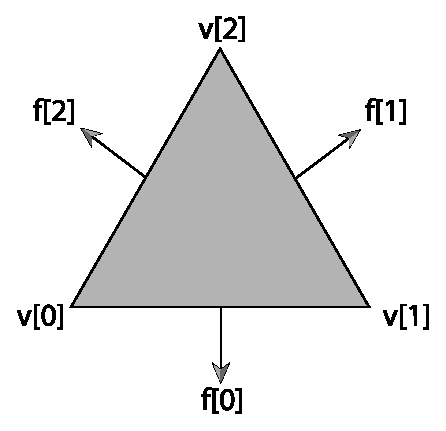
\includegraphics[width=0.35\linewidth]{chap03/Subdivvertfacepointers.eps}
    \caption{每个三角形面存有三个指向\protect\refvar{SDVertex}{}对象的
    指针{\ttfamily\protect\refvar[SDFace::v]{v}{}[i]}以及三个
    指向相邻面的指针{\ttfamily\protect\refvar[SDFace::f]{f}{}[i]}。
    相邻面索引使用的约定是第{\ttfamily i}边是
    从{\ttfamily\protect\refvar[SDFace::v]{v}{}[i]}到{\ttfamily\protect\refvar[SDFace::v]{v}{}[(i+1)\%3]}的边,
    且第{\ttfamily i}边的邻居在{\ttfamily\protect\refvar[SDFace::f]{f}{}[i]}中。}
    \label{fig:3.27}
\end{figure}

\begin{lstlisting}
`\refcode{LoopSubdiv Local Structures}{+=}\lastnext{LoopSubdivLocalStructures}`
struct `\initvar{SDFace}{}` {
    `\refcode{SDFace Constructor}{}`
    `\refcode{SDFace Methods}{}`
    `\refvar{SDVertex}{}` *`\initvar[SDFace::v]{v}{}`[3];
    `\refvar{SDFace}{}` *`\initvar[SDFace::f]{f}{}`[3];
    `\refvar{SDFace}{}` *`\initvar{children}{}`[4];
};
\end{lstlisting}

\refvar{SDFace}{}构造函数很简单——它简单地把这些不同的指针设置为{\ttfamily nullptr}——
所以这里不再展示。

为简化\refvar{SDFace}{}的数据结构导航,
我们提供宏使得决定特定索引前后的顶点和面索引更容易。
这些宏添加适合的偏移量并计算模三结果以负责循环。
\begin{lstlisting}
`\initcode{LoopSubdiv Macros}{=}`
#define `\initvar{NEXT}{}`(i) (((i) + 1) % 3)
#define `\initvar{PREV}{}`(i) (((i) + 2) % 3)
\end{lstlisting}

除了需要流形网格外,细分代码希望用户指定的控制网格
是\keyindex{相容次序}{consistently ordered}{}的——
网格中每条\keyindex{有向边}{directed edge}{edge边}只出现一次。
两个面的公共边须由每个面指定为不同方向。
考虑两个顶点$\bm v_0$和$\bm v_1$与连接它们的边。
我们希望拥有该边的三角形面指定其三个顶点时$\bm v_0$在$\bm v_1$之前,
另一个面指定顶点时$\bm v_1$在$\bm v_0$之前(\reffig{3.28})。
\keyindex{莫比乌斯带}{Möbius strip}{}是无法相容次序的曲面例子,
但渲染中几乎不会遇到这样的曲面,所以实践中该限制没问题。
然而不能创建相容次序网格的程序给出的没构建好的网格数据可能会造成问题。
\begin{figure}[htbp]
    \centering%LaTeX with PSTricks extensions
%%Creator: Inkscape 1.0.1 (3bc2e813f5, 2020-09-07)
%%Please note this file requires PSTricks extensions
\psset{xunit=.4pt,yunit=.4pt,runit=.4pt}
\begin{pspicture}(341.97000122,255.44999695)
{
\newrgbcolor{curcolor}{0 0 0}
\pscustom[linewidth=1,linecolor=curcolor]
{
\newpath
\moveto(127.34,36.99999695)
\lineto(126.89,36.93999695)
\lineto(32.5,23.00999695)
\lineto(67.63,111.70999695)
}
}
{
\newrgbcolor{curcolor}{0 0 0}
\pscustom[linestyle=none,fillstyle=solid,fillcolor=curcolor]
{
\newpath
\moveto(121.67,41.72999695)
\lineto(126.69,36.90999695)
\lineto(123.28,30.83999695)
\lineto(135.35,38.18999695)
\closepath
}
}
{
\newrgbcolor{curcolor}{0.65098041 0.65098041 0.65098041}
\pscustom[linestyle=none,fillstyle=solid,fillcolor=curcolor]
{
\newpath
\moveto(123.39,40.76999695)
\lineto(134.06,37.98999695)
\lineto(127.32,36.99999695)
\closepath
}
}
{
\newrgbcolor{curcolor}{0.40000001 0.40000001 0.40000001}
\pscustom[linestyle=none,fillstyle=solid,fillcolor=curcolor]
{
\newpath
\moveto(124.65,32.25999695)
\lineto(134.06,37.98999695)
\lineto(127.32,36.99999695)
\closepath
}
}
{
\newrgbcolor{curcolor}{0 0 0}
\pscustom[linewidth=1,linecolor=curcolor]
{
\newpath
\moveto(67.63,111.70999695)
\lineto(102.77,200.41999695)
\lineto(162.02,125.63999695)
\lineto(162.59,124.91999695)
}
}
{
\newrgbcolor{curcolor}{0 0 0}
\pscustom[linestyle=none,fillstyle=solid,fillcolor=curcolor]
{
\newpath
\moveto(74.56,114.24999695)
\lineto(67.87,112.31999695)
\lineto(64.32,118.30999695)
\lineto(64.65,104.17999695)
\closepath
}
}
{
\newrgbcolor{curcolor}{0.65098041 0.65098041 0.65098041}
\pscustom[linestyle=none,fillstyle=solid,fillcolor=curcolor]
{
\newpath
\moveto(72.87,113.24999695)
\lineto(65.13,105.39999695)
\lineto(67.64,111.72999695)
\closepath
}
}
{
\newrgbcolor{curcolor}{0.40000001 0.40000001 0.40000001}
\pscustom[linestyle=none,fillstyle=solid,fillcolor=curcolor]
{
\newpath
\moveto(64.87,116.40999695)
\lineto(65.13,105.39999695)
\lineto(67.64,111.72999695)
\closepath
}
}
{
\newrgbcolor{curcolor}{0 0 0}
\pscustom[linewidth=1,linecolor=curcolor]
{
\newpath
\moveto(162.59,124.91999695)
\lineto(221.28,50.86999695)
\lineto(133.97,37.97999695)
}
}
{
\newrgbcolor{curcolor}{0 0 0}
\pscustom[linestyle=none,fillstyle=solid,fillcolor=curcolor]
{
\newpath
\moveto(161.33,117.65999695)
\lineto(163,124.40999695)
\lineto(169.95,124.48999695)
\lineto(157.56,131.27999695)
\closepath
}
}
{
\newrgbcolor{curcolor}{0.65098041 0.65098041 0.65098041}
\pscustom[linestyle=none,fillstyle=solid,fillcolor=curcolor]
{
\newpath
\moveto(161.3,119.62999695)
\lineto(158.37,130.24999695)
\lineto(162.6,124.90999695)
\closepath
}
}
{
\newrgbcolor{curcolor}{0.40000001 0.40000001 0.40000001}
\pscustom[linestyle=none,fillstyle=solid,fillcolor=curcolor]
{
\newpath
\moveto(168.04,124.96999695)
\lineto(158.37,130.24999695)
\lineto(162.6,124.90999695)
\closepath
}
}
{
\newrgbcolor{curcolor}{0 0 0}
\pscustom[linewidth=1,linecolor=curcolor]
{
\newpath
\moveto(270.07,144.47999695)
\lineto(269.9,144.05999695)
\lineto(234.64,55.40999695)
\lineto(175.5,130.26999695)
}
}
{
\newrgbcolor{curcolor}{0 0 0}
\pscustom[linestyle=none,fillstyle=solid,fillcolor=curcolor]
{
\newpath
\moveto(263.14,141.94999695)
\lineto(269.83,143.86999695)
\lineto(273.37,137.87999695)
\lineto(273.07,152.00999695)
\closepath
}
}
{
\newrgbcolor{curcolor}{0.65098041 0.65098041 0.65098041}
\pscustom[linestyle=none,fillstyle=solid,fillcolor=curcolor]
{
\newpath
\moveto(264.83,142.94999695)
\lineto(272.58,150.78999695)
\lineto(270.06,144.45999695)
\closepath
}
}
{
\newrgbcolor{curcolor}{0.40000001 0.40000001 0.40000001}
\pscustom[linestyle=none,fillstyle=solid,fillcolor=curcolor]
{
\newpath
\moveto(272.82,139.76999695)
\lineto(272.58,150.78999695)
\lineto(270.06,144.45999695)
\closepath
}
}
{
\newrgbcolor{curcolor}{0 0 0}
\pscustom[linewidth=1,linecolor=curcolor]
{
\newpath
\moveto(175.5,130.26999695)
\lineto(116.35,205.13999695)
\lineto(210.76,218.92999695)
\lineto(211.67,219.05999695)
}
}
{
\newrgbcolor{curcolor}{0 0 0}
\pscustom[linestyle=none,fillstyle=solid,fillcolor=curcolor]
{
\newpath
\moveto(176.77,137.53999695)
\lineto(175.09,130.77999695)
\lineto(168.13,130.71999695)
\lineto(180.52,123.91999695)
\closepath
}
}
{
\newrgbcolor{curcolor}{0.65098041 0.65098041 0.65098041}
\pscustom[linestyle=none,fillstyle=solid,fillcolor=curcolor]
{
\newpath
\moveto(176.79,135.56999695)
\lineto(179.71,124.94999695)
\lineto(175.48,130.28999695)
\closepath
}
}
{
\newrgbcolor{curcolor}{0.40000001 0.40000001 0.40000001}
\pscustom[linestyle=none,fillstyle=solid,fillcolor=curcolor]
{
\newpath
\moveto(170.05,130.23999695)
\lineto(179.71,124.94999695)
\lineto(175.48,130.28999695)
\closepath
}
}
{
\newrgbcolor{curcolor}{0 0 0}
\pscustom[linewidth=1,linecolor=curcolor]
{
\newpath
\moveto(211.67,219.05999695)
\lineto(305.17,232.70999695)
\lineto(272.55,150.70999695)
}
}
{
\newrgbcolor{curcolor}{0 0 0}
\pscustom[linestyle=none,fillstyle=solid,fillcolor=curcolor]
{
\newpath
\moveto(217.32,214.31999695)
\lineto(212.31,219.14999695)
\lineto(215.74,225.20999695)
\lineto(203.65,217.88999695)
\closepath
}
}
{
\newrgbcolor{curcolor}{0.65098041 0.65098041 0.65098041}
\pscustom[linestyle=none,fillstyle=solid,fillcolor=curcolor]
{
\newpath
\moveto(215.61,215.28999695)
\lineto(204.95,218.07999695)
\lineto(211.69,219.05999695)
\closepath
}
}
{
\newrgbcolor{curcolor}{0.40000001 0.40000001 0.40000001}
\pscustom[linestyle=none,fillstyle=solid,fillcolor=curcolor]
{
\newpath
\moveto(214.37,223.78999695)
\lineto(204.95,218.07999695)
\lineto(211.69,219.05999695)
\closepath
}
}
{
\newrgbcolor{curcolor}{0 0 0}
\pscustom[linestyle=none,fillstyle=solid,fillcolor=curcolor]
{
\newpath
\moveto(103.41623732,220.6309431)
\curveto(103.41623732,222.8059431)(101.80373732,222.8059431)(101.80373732,222.8059431)
\curveto(100.82873732,222.8059431)(99.96623732,221.7934431)(99.96623732,221.0059431)
\curveto(99.96623732,220.3309431)(100.49123732,220.0309431)(100.67873732,219.9184431)
\curveto(101.69123732,219.3184431)(101.87873732,218.8684431)(101.87873732,218.4184431)
\curveto(101.87873732,217.8934431)(100.49123732,212.6434431)(97.71623732,212.6434431)
\curveto(95.99123732,212.6434431)(95.99123732,214.0684431)(95.99123732,214.5184431)
\curveto(95.99123732,215.9059431)(96.66623732,217.6309431)(97.41623732,219.5434431)
\curveto(97.60373732,220.0309431)(97.67873732,220.2559431)(97.67873732,220.6309431)
\curveto(97.67873732,222.0184431)(96.29123732,222.7684431)(94.97873732,222.7684431)
\curveto(92.42873732,222.7684431)(91.22873732,219.5434431)(91.22873732,219.0559431)
\curveto(91.22873732,218.7184431)(91.60373732,218.7184431)(91.82873732,218.7184431)
\curveto(92.09123732,218.7184431)(92.27873732,218.7184431)(92.35373732,219.0184431)
\curveto(93.14123732,221.6059431)(94.41623732,221.9059431)(94.82873732,221.9059431)
\curveto(95.01623732,221.9059431)(95.24123732,221.9059431)(95.24123732,221.4184431)
\curveto(95.24123732,220.8559431)(94.94123732,220.1809431)(94.86623732,219.9934431)
\curveto(93.77873732,217.2184431)(93.40373732,216.1309431)(93.40373732,214.9684431)
\curveto(93.40373732,212.4559431)(95.46623732,211.7809431)(97.56623732,211.7809431)
\curveto(101.69123732,211.7809431)(103.41623732,218.5684431)(103.41623732,220.6309431)
\closepath
\moveto(103.41623732,220.6309431)
}
}
{
\newrgbcolor{curcolor}{0 0 0}
\pscustom[linestyle=none,fillstyle=solid,fillcolor=curcolor]
{
\newpath
\moveto(112.65412795,213.70783519)
\curveto(112.65412795,215.54533519)(112.42912795,216.89533519)(111.67912795,218.05783519)
\curveto(111.15412795,218.80783519)(110.10412795,219.48283519)(108.79162795,219.48283519)
\curveto(104.89162795,219.48283519)(104.89162795,214.90783519)(104.89162795,213.70783519)
\curveto(104.89162795,212.50783519)(104.89162795,208.04533519)(108.79162795,208.04533519)
\curveto(112.65412795,208.04533519)(112.65412795,212.50783519)(112.65412795,213.70783519)
\closepath
\moveto(108.79162795,208.53283519)
\curveto(108.00412795,208.53283519)(106.99162795,208.98283519)(106.65412795,210.33283519)
\curveto(106.42912795,211.30783519)(106.42912795,212.69533519)(106.42912795,213.93283519)
\curveto(106.42912795,215.17033519)(106.42912795,216.44533519)(106.65412795,217.34533519)
\curveto(107.02912795,218.65783519)(108.07912795,219.03283519)(108.79162795,219.03283519)
\curveto(109.69162795,219.03283519)(110.55412795,218.47033519)(110.85412795,217.49533519)
\curveto(111.11662795,216.59533519)(111.15412795,215.39533519)(111.15412795,213.93283519)
\curveto(111.15412795,212.69533519)(111.15412795,211.45783519)(110.92912795,210.40783519)
\curveto(110.59162795,208.87033519)(109.46662795,208.53283519)(108.79162795,208.53283519)
\closepath
\moveto(108.79162795,208.53283519)
}
}
{
\newrgbcolor{curcolor}{0 0 0}
\pscustom[linestyle=none,fillstyle=solid,fillcolor=curcolor]
{
\newpath
\moveto(238.94984342,45.3926351)
\curveto(238.94984342,47.5676351)(237.33734342,47.5676351)(237.33734342,47.5676351)
\curveto(236.36234342,47.5676351)(235.49984342,46.5551351)(235.49984342,45.7676351)
\curveto(235.49984342,45.0926351)(236.02484342,44.7926351)(236.21234342,44.6801351)
\curveto(237.22484342,44.0801351)(237.41234342,43.6301351)(237.41234342,43.1801351)
\curveto(237.41234342,42.6551351)(236.02484342,37.4051351)(233.24984342,37.4051351)
\curveto(231.52484342,37.4051351)(231.52484342,38.8301351)(231.52484342,39.2801351)
\curveto(231.52484342,40.6676351)(232.19984342,42.3926351)(232.94984342,44.3051351)
\curveto(233.13734342,44.7926351)(233.21234342,45.0176351)(233.21234342,45.3926351)
\curveto(233.21234342,46.7801351)(231.82484342,47.5301351)(230.51234342,47.5301351)
\curveto(227.96234342,47.5301351)(226.76234342,44.3051351)(226.76234342,43.8176351)
\curveto(226.76234342,43.4801351)(227.13734342,43.4801351)(227.36234342,43.4801351)
\curveto(227.62484342,43.4801351)(227.81234342,43.4801351)(227.88734342,43.7801351)
\curveto(228.67484342,46.3676351)(229.94984342,46.6676351)(230.36234342,46.6676351)
\curveto(230.54984342,46.6676351)(230.77484342,46.6676351)(230.77484342,46.1801351)
\curveto(230.77484342,45.6176351)(230.47484342,44.9426351)(230.39984342,44.7551351)
\curveto(229.31234342,41.9801351)(228.93734342,40.8926351)(228.93734342,39.7301351)
\curveto(228.93734342,37.2176351)(230.99984342,36.5426351)(233.09984342,36.5426351)
\curveto(237.22484342,36.5426351)(238.94984342,43.3301351)(238.94984342,45.3926351)
\closepath
\moveto(238.94984342,45.3926351)
}
}
{
\newrgbcolor{curcolor}{0 0 0}
\pscustom[linestyle=none,fillstyle=solid,fillcolor=curcolor]
{
\newpath
\moveto(245.15023405,43.79452719)
\curveto(245.15023405,44.24452719)(245.15023405,44.24452719)(244.66273405,44.24452719)
\curveto(243.57523405,43.19452719)(242.07523405,43.19452719)(241.40023405,43.19452719)
\lineto(241.40023405,42.59452719)
\curveto(241.77523405,42.59452719)(242.90023405,42.59452719)(243.80023405,43.04452719)
\lineto(243.80023405,34.53202719)
\curveto(243.80023405,33.96952719)(243.80023405,33.74452719)(242.15023405,33.74452719)
\lineto(241.51273405,33.74452719)
\lineto(241.51273405,33.14452719)
\curveto(241.81273405,33.14452719)(243.87523405,33.21952719)(244.47523405,33.21952719)
\curveto(245.00023405,33.21952719)(247.10023405,33.14452719)(247.47523405,33.14452719)
\lineto(247.47523405,33.74452719)
\lineto(246.83773405,33.74452719)
\curveto(245.15023405,33.74452719)(245.15023405,33.96952719)(245.15023405,34.53202719)
\closepath
\moveto(245.15023405,43.79452719)
}
}
{
\newrgbcolor{curcolor}{0 0 0}
\pscustom[linestyle=none,fillstyle=solid,fillcolor=curcolor]
{
\newpath
\moveto(318.40669232,246.1308431)
\curveto(318.40669232,248.3058431)(316.79419232,248.3058431)(316.79419232,248.3058431)
\curveto(315.81919232,248.3058431)(314.95669232,247.2933431)(314.95669232,246.5058431)
\curveto(314.95669232,245.8308431)(315.48169232,245.5308431)(315.66919232,245.4183431)
\curveto(316.68169232,244.8183431)(316.86919232,244.3683431)(316.86919232,243.9183431)
\curveto(316.86919232,243.3933431)(315.48169232,238.1433431)(312.70669232,238.1433431)
\curveto(310.98169232,238.1433431)(310.98169232,239.5683431)(310.98169232,240.0183431)
\curveto(310.98169232,241.4058431)(311.65669232,243.1308431)(312.40669232,245.0433431)
\curveto(312.59419232,245.5308431)(312.66919232,245.7558431)(312.66919232,246.1308431)
\curveto(312.66919232,247.5183431)(311.28169232,248.2683431)(309.96919232,248.2683431)
\curveto(307.41919232,248.2683431)(306.21919232,245.0433431)(306.21919232,244.5558431)
\curveto(306.21919232,244.2183431)(306.59419232,244.2183431)(306.81919232,244.2183431)
\curveto(307.08169232,244.2183431)(307.26919232,244.2183431)(307.34419232,244.5183431)
\curveto(308.13169232,247.1058431)(309.40669232,247.4058431)(309.81919232,247.4058431)
\curveto(310.00669232,247.4058431)(310.23169232,247.4058431)(310.23169232,246.9183431)
\curveto(310.23169232,246.3558431)(309.93169232,245.6808431)(309.85669232,245.4933431)
\curveto(308.76919232,242.7183431)(308.39419232,241.6308431)(308.39419232,240.4683431)
\curveto(308.39419232,237.9558431)(310.45669232,237.2808431)(312.55669232,237.2808431)
\curveto(316.68169232,237.2808431)(318.40669232,244.0683431)(318.40669232,246.1308431)
\closepath
\moveto(318.40669232,246.1308431)
}
}
{
\newrgbcolor{curcolor}{0 0 0}
\pscustom[linestyle=none,fillstyle=solid,fillcolor=curcolor]
{
\newpath
\moveto(327.45708295,236.92023519)
\lineto(326.89458295,236.92023519)
\curveto(326.85708295,236.54523519)(326.66958295,235.57023519)(326.44458295,235.42023519)
\curveto(326.33208295,235.30773519)(325.05708295,235.30773519)(324.79458295,235.30773519)
\lineto(321.71958295,235.30773519)
\curveto(323.48208295,236.84523519)(324.08208295,237.33273519)(325.05708295,238.12023519)
\curveto(326.29458295,239.09523519)(327.45708295,240.14523519)(327.45708295,241.72023519)
\curveto(327.45708295,243.74523519)(325.69458295,244.98273519)(323.55708295,244.98273519)
\curveto(321.49458295,244.98273519)(320.06958295,243.52023519)(320.06958295,241.98273519)
\curveto(320.06958295,241.15773519)(320.78208295,241.04523519)(320.96958295,241.04523519)
\curveto(321.34458295,241.04523519)(321.83208295,241.34523519)(321.83208295,241.94523519)
\curveto(321.83208295,242.24523519)(321.71958295,242.84523519)(320.85708295,242.84523519)
\curveto(321.38208295,244.00773519)(322.50708295,244.38273519)(323.29458295,244.38273519)
\curveto(324.98208295,244.38273519)(325.84458295,243.07023519)(325.84458295,241.72023519)
\curveto(325.84458295,240.25773519)(324.79458295,239.13273519)(324.26958295,238.53273519)
\lineto(320.25708295,234.52023519)
\curveto(320.06958295,234.37023519)(320.06958295,234.33273519)(320.06958295,233.88273519)
\lineto(326.96958295,233.88273519)
\closepath
\moveto(327.45708295,236.92023519)
}
}
{
\newrgbcolor{curcolor}{0 0 0}
\pscustom[linestyle=none,fillstyle=solid,fillcolor=curcolor]
{
\newpath
\moveto(20.76141732,19.7093961)
\curveto(20.76141732,21.8843961)(19.14891732,21.8843961)(19.14891732,21.8843961)
\curveto(18.17391732,21.8843961)(17.31141732,20.8718961)(17.31141732,20.0843961)
\curveto(17.31141732,19.4093961)(17.83641732,19.1093961)(18.02391732,18.9968961)
\curveto(19.03641732,18.3968961)(19.22391732,17.9468961)(19.22391732,17.4968961)
\curveto(19.22391732,16.9718961)(17.83641732,11.7218961)(15.06141732,11.7218961)
\curveto(13.33641732,11.7218961)(13.33641732,13.1468961)(13.33641732,13.5968961)
\curveto(13.33641732,14.9843961)(14.01141732,16.7093961)(14.76141732,18.6218961)
\curveto(14.94891732,19.1093961)(15.02391732,19.3343961)(15.02391732,19.7093961)
\curveto(15.02391732,21.0968961)(13.63641732,21.8468961)(12.32391732,21.8468961)
\curveto(9.77391732,21.8468961)(8.57391732,18.6218961)(8.57391732,18.1343961)
\curveto(8.57391732,17.7968961)(8.94891732,17.7968961)(9.17391732,17.7968961)
\curveto(9.43641732,17.7968961)(9.62391732,17.7968961)(9.69891732,18.0968961)
\curveto(10.48641732,20.6843961)(11.76141732,20.9843961)(12.17391732,20.9843961)
\curveto(12.36141732,20.9843961)(12.58641732,20.9843961)(12.58641732,20.4968961)
\curveto(12.58641732,19.9343961)(12.28641732,19.2593961)(12.21141732,19.0718961)
\curveto(11.12391732,16.2968961)(10.74891732,15.2093961)(10.74891732,14.0468961)
\curveto(10.74891732,11.5343961)(12.81141732,10.8593961)(14.91141732,10.8593961)
\curveto(19.03641732,10.8593961)(20.76141732,17.6468961)(20.76141732,19.7093961)
\closepath
\moveto(20.76141732,19.7093961)
}
}
{
\newrgbcolor{curcolor}{0 0 0}
\pscustom[linestyle=none,fillstyle=solid,fillcolor=curcolor]
{
\newpath
\moveto(25.94930795,13.04878819)
\curveto(27.26180795,13.04878819)(28.19930795,12.14878819)(28.19930795,10.34878819)
\curveto(28.19930795,8.28628819)(26.96180795,7.64878819)(26.02430795,7.64878819)
\curveto(25.34930795,7.64878819)(23.84930795,7.83628819)(23.17430795,8.84878819)
\curveto(23.96180795,8.84878819)(24.14930795,9.41128819)(24.14930795,9.78628819)
\curveto(24.14930795,10.31128819)(23.73680795,10.68628819)(23.21180795,10.68628819)
\curveto(22.76180795,10.68628819)(22.27430795,10.38628819)(22.27430795,9.71128819)
\curveto(22.27430795,8.13628819)(23.99930795,7.12378819)(26.02430795,7.12378819)
\curveto(28.34930795,7.12378819)(29.96180795,8.69878819)(29.96180795,10.34878819)
\curveto(29.96180795,11.66128819)(28.91180795,12.97378819)(27.07430795,13.34878819)
\curveto(28.79930795,13.98628819)(29.43680795,15.22378819)(29.43680795,16.27378819)
\curveto(29.43680795,17.58628819)(27.93680795,18.56128819)(26.06180795,18.56128819)
\curveto(24.22430795,18.56128819)(22.79930795,17.66128819)(22.79930795,16.31128819)
\curveto(22.79930795,15.74878819)(23.17430795,15.44878819)(23.66180795,15.44878819)
\curveto(24.18680795,15.44878819)(24.52430795,15.82378819)(24.52430795,16.27378819)
\curveto(24.52430795,16.76128819)(24.18680795,17.13628819)(23.66180795,17.17378819)
\curveto(24.26180795,17.88628819)(25.38680795,18.07378819)(26.02430795,18.07378819)
\curveto(26.77430795,18.07378819)(27.82430795,17.69878819)(27.82430795,16.27378819)
\curveto(27.82430795,15.56128819)(27.59930795,14.77378819)(27.14930795,14.28628819)
\curveto(26.62430795,13.64878819)(26.13680795,13.61128819)(25.31180795,13.53628819)
\curveto(24.89930795,13.49878819)(24.86180795,13.49878819)(24.78680795,13.49878819)
\curveto(24.74930795,13.49878819)(24.59930795,13.46128819)(24.59930795,13.27378819)
\curveto(24.59930795,13.04878819)(24.74930795,13.04878819)(25.04930795,13.04878819)
\closepath
\moveto(25.94930795,13.04878819)
}
}
\end{pspicture}

    \caption{输入网格中的所有面必须指定为让每条公共边在每个方向最多出现一次。
        这里,从$\bm v_0$到$\bm v_1$的边被一个面从$\bm v_0$到$\bm v_1$穿过
        而被另一个面从$\bm v_1$到$\bm v_0$穿过。
        另一个看待方式是考虑面朝向:从网格外边观察时,
        所有面的顶点应该统一地以顺时针或逆时针顺序给出。}
    \label{fig:3.28}
\end{figure}

有了关于输入数据的该假设,\refvar{LoopSubdivide}{()}现在
可以初始化网格的拓扑数据结构了。
它首先遍历所有面并设置它们的指针\refvar[SDFace::v]{v}{}指向它们的三个顶点。
它还设置每个顶点的指针\refvar[startFace]{SDVertex::startFace}{}指向
该顶点相邻面中的一个。具体使用哪一个相邻面并不重要,
所以每次遇到该顶点关联的另一个面时,该实现就重设它,
这条保证所有顶点在遍历完成前都有非空的面指针。
\begin{lstlisting}
`\initcode{Set face to vertex pointers}{=}`
const int *vp = vertexIndices;
for (int i = 0; i < nFaces; ++i, vp += 3) {
    SDFace *f = faces[i];
    for (int j = 0; j < 3; ++j) {
        SDVertex *v = vertices[vp[j]];
        f->`\refvar[SDFace::v]{v}{}`[j] = v;
        v->`\refvar{startFace}{}` = f;
    }
}
\end{lstlisting}

现在有必要将每个面的\refvar[SDFace::f]{f}{}指针设置为指向其相邻面。
这有些棘手,因为传入
\refvar{LoopSubdivide}{()}的数据并不直接指定面的相邻信息。
这里的实现遍历面并为其三条边的每一条都创建\refvar{SDEdge}{}对象。
当遇到另一个面共享同一边时,它就更新两个面的相邻指针。
\begin{lstlisting}
`\refcode{LoopSubdiv Local Structures}{+=}\lastcode{LoopSubdivLocalStructures}`
struct `\initvar{SDEdge}{}` {
    `\refcode{SDEdge Constructor}{}`
    `\refcode{SDEdge Comparison Function}{}`
    `\refvar{SDVertex}{}` *`\initvar[SDEdge::v]{v}{}`[2];
    `\refvar{SDFace}{}` *`\initvar[SDEdge::f]{f}{}`[2];
    int `\initvar{f0edgeNum}{}`;
};
\end{lstlisting}

\refvar{SDEdge}{}构造函数接收指向边的两端顶点的指针。
它对指针排序使得{\ttfamily\refvar[SDEdge::v]{v}{}[0]}是
排在内存中最前面的那个。这段代码可能看起来很奇怪,
但它简单依赖于这样的事实即C++中的指针是可以像整数那样高效操作的数字
\footnote{尽管是分段架构。}而一边的顶点顺序是任意的。
基于其指针地址排列这两个顶点保证了边$(\bm v_a,\bm v_b)$可以
被正确认作和边$(\bm v_b,\bm v_a)$相同,而不管提供的顶点顺序是什么。
\begin{lstlisting}
`\initcode{SDEdge Constructor}{=}`
`\refvar{SDEdge}{}`(`\refvar{SDVertex}{}` *v0 = nullptr, `\refvar{SDVertex}{}` *v1 = nullptr) {
    `\refvar[SDEdge::v]{v}{}`[0] = std::min(v0, v1);
    `\refvar[SDEdge::v]{v}{}`[1] = std::max(v0, v1);
    `\refvar[SDEdge::f]{f}{}`[0] = `\refvar[SDEdge::f]{f}{}`[1] = nullptr;
    `\refvar{f0edgeNum}{}` = -1;
}
\end{lstlisting}

该类还定义了\refvar{SDEdge}{}对象的排序操作
这样它们就能存于其他依赖良好顺序定义的数据结构。
\begin{lstlisting}
`\initcode{SDEdge Comparison Function}{=}`
bool operator<(const `\refvar{SDEdge}{}` &e2) const {
    if (`\refvar[SDEdge::v]{v}{}`[0] == e2.`\refvar[SDEdge::v]{v}{}`[0]) return `\refvar[SDEdge::v]{v}{}`[1] < e2.`\refvar[SDEdge::v]{v}{}`[1];
    return `\refvar[SDEdge::v]{v}{}`[0] < e2.`\refvar[SDEdge::v]{v}{}`[0];
}
\end{lstlisting}

现在函数\refvar{LoopSubdivide}{()}可以开始工作了,
遍历所有面的边并随之更新相邻指针。
它用{\ttfamily set}存储目前只有一个相邻面的边。
{\ttfamily set}让在$O(\log{n})$时间内搜索特定边成为可能。
\begin{lstlisting}
`\initcode{Set neighbor pointers in faces}{=}`
std::set<`\refvar{SDEdge}{}`> edges;
for (int i = 0; i < nFaces; ++i) {
    `\refvar{SDFace}{}` *f = faces[i];
    for (int edgeNum = 0; edgeNum < 3; ++edgeNum) {
        `\refcode{Update neighbor pointer for edgeNum}{}`
    }
}
\end{lstlisting}

对于每个面中的每条边,循环体创建一个边对象并检查之前是否已经见过同样的边。
如果是,它就初始化共享该边的两个面的相邻指针。
如果否,它就将该边添加到边的集合中。
该边两端两个顶点的索引{\ttfamily v0}和{\ttfamily v1},
分别等于边的索引和边的边的索引加一。
\begin{lstlisting}
`\initcode{Update neighbor pointer for edgeNum}{=}`
int v0 = edgeNum, v1 = `\refvar{NEXT}{}`(edgeNum);
`\refvar{SDEdge}{}` e(f->`\refvar[SDFace::v]{v}{}`[v0], f->`\refvar[SDFace::v]{v}{}`[v1]);
if (edges.find(e) == edges.end()) {
    `\refcode{Handle new edge}{}`
} else {
    `\refcode{Handle previously seen edge}{}`
}
\end{lstlisting}

给定之前没遇到的边,当前的面的指针存储于边对象的成员{\ttfamily\refvar[SDEdge::f]{f}{}[0]}中。
因为假设输入网格是流形,所以最多还有另一个面共享这条边。
当发现该面时,可以用它初始化相邻面的域。
在当前的面中存储该边的号码能让相邻面初始化其相应相邻边的指针。
\begin{lstlisting}
`\initcode{Handle new edge}{=}`
e.`\refvar[SDEdge::f]{f}{}`[0] = f;
e.`\refvar{f0edgeNum}{}` = edgeNum;
edges.insert(e);
\end{lstlisting}

当找到该边上的第二个面时,两个面都设置相邻指针。
然后从边的集合中移除该边,因为没有边可以被两个以上的面共享。
\begin{lstlisting}
`\initcode{Handle previously seen edge}{=}`
e = *edges.find(e);
e.`\refvar[SDEdge::f]{f}{}`[0]->`\refvar[SDFace::f]{f}{}`[e.`\refvar{f0edgeNum}{}`] = f;
f->`\refvar[SDFace::f]{f}{}`[edgeNum] = e.`\refvar[SDEdge::f]{f}{}`[0];
edges.erase(e);
\end{lstlisting}

现在所有面都有合适的相邻指针,
可以设置每个顶点中的标志\refvar[SDVertex::boundary]{boundary}{}和
\refvar{regular}{}了。为了确定顶点是否是边界顶点,我们将定义围绕顶点的面顺序(\reffig{3.29})。
对于面{\ttfamily f}上的顶点{\ttfamily\refvar[SDFace::v]{v}{}[i]},
我们定义顶点的\emph{下一面}是邻接从{\ttfamily\refvar[SDFace::v]{v}{}[i]}到{\ttfamily\refvar[SDFace::v]{v}{}[\refvar{NEXT}{}(i)]}的边的面,
\emph{上一面}是邻接从{\ttfamily\refvar[SDFace::v]{v}{}[\refvar{PREV}{}(i)]}到{\ttfamily\refvar[SDFace::v]{v}{}[i]}的边的面。
\begin{figure}[htbp]
    \centering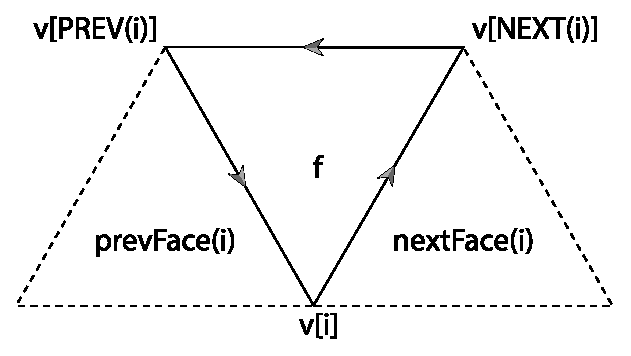
\includegraphics[width=0.4\linewidth]{chap03/Subdivprevnextface.eps}
    \caption{给定顶点{\ttfamily\refvar[SDFace::v]{v}{}[i]}和附带的面{\ttfamily f},
    我们定义\emph{下一面}为与{\ttfamily f}通过
    从{\ttfamily\protect\refvar[SDFace::v]{v}{}[i]}到{\ttfamily\protect\refvar[SDFace::v]{v}{}[\protect\refvar{NEXT}{}(i)]}的边邻接的面。
    上一面的定义类似。}
    \label{fig:3.29}
\end{figure}

通过依次转到围绕\refvar[SDFace::v]{v}{}的下一面,
我们可以遍历与之相邻的面。
如果我们最终回到出发的面,则我们位于内部顶点上;
如果我们遇到一条边的相邻指针是{\ttfamily nullptr},
则我们位于边界顶点上(\reffig{3.30})。
一旦初始化例程确定这是否是边界顶点,
它就计算顶点的价,如果是价为6的内部顶点或价为4的边界顶点,
就置位标志\refvar{regular}{};否则这是个非凡顶点。
\begin{figure}[htbp]
    \centering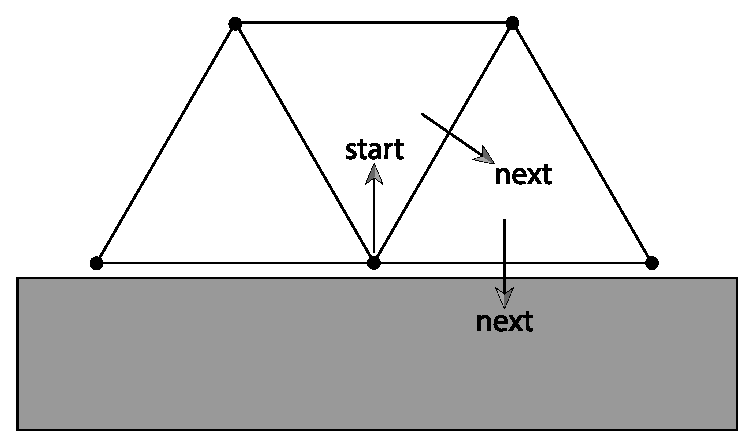
\includegraphics[width=0.5\linewidth]{chap03/Subdivdetermineboundary.eps}
    \caption{我们可以通过从相邻面\protect\refvar{startFace}{}开始
        并跟随围绕该顶点的下一面指针来确定一个顶点是否是边界顶点。
        如果我们遇到一个没有下一相邻面的面,则该顶点在边界上。
        如果我们回到\protect\refvar{startFace}{},则它是内部顶点。}
    \label{fig:3.30}
\end{figure}

\begin{lstlisting}
`\initcode{Finish vertex initialization}{=}`
for (int i = 0; i < nVertices; ++i) {
    `\refvar{SDVertex}{}` *v = vertices[i];
    `\refvar{SDFace}{}` *f = v->`\refvar{startFace}{}`;
    do {
        f = f->`\refvar{nextFace}{}`(v);
    } while (f && f != v->`\refvar{startFace}{}`);
    v->`\refvar[SDVertex::boundary]{boundary}{}` = (f == nullptr);
    if (!v->`\refvar[SDVertex::boundary]{boundary}{}` && v->`\refvar{valence}{}`() == 6)
        v->`\refvar{regular}{}` = true;
    else if (v->`\refvar[SDVertex::boundary]{boundary}{}` && v->`\refvar{valence}{}`() == 4)
        v->`\refvar{regular}{}` = true;
    else
        v->`\refvar{regular}{}` = false;
}
\end{lstlisting}

因为经常需要顶点的价,所以我们提供方法\refvar[valence]{SDVertex::valence}{()}。
\begin{lstlisting}
`\initcode{LoopSubdiv Inline Functions}{=}\initnext{LoopSubdivInlineFunctions}`
inline int `\refvar{SDVertex}{}`::`\initvar{valence}{}`() {
    `\refvar{SDFace}{}` *f = `\refvar{startFace}{}`;
    if (!`\refvar[SDVertex::boundary]{boundary}{}`) {
        `\refcode{Compute valence of interior vertex}{}`
    } else {
        `\refcode{Compute valence of boundary vertex}{}`
    }
}
\end{lstlisting}

为了计算非边界顶点的价,该方法跟随每个面围绕该顶点的相邻指针
开始计算相邻面的数量,直到它回到出发的面。
价等于访问的面的数量。
\begin{lstlisting}
`\initcode{Compute valence of interior vertex}{=}`
int nf = 1;
while ((f = f->`\refvar{nextFace}{}`(this)) != `\refvar{startFace}{}`)
    ++nf;
return nf;
\end{lstlisting}

对于边界顶点我们可以用相同的方法,但这种情况下价比相邻面的数量多一。
这里遍历相邻面稍微更复杂些:它跟随围绕该顶点的下一面指针直到遇到边界,计算见过的面的数量。
然后它再次从\refvar{startFace}{}开始并跟随上一面指针直到在另一方向遇到边界。
\begin{lstlisting}
`\initcode{Compute valence of boundary vertex}{=}`
int nf = 1;
while ((f = f->`\refvar{nextFace}{}`(this)) != nullptr)
    ++nf;
f = `\refvar{startFace}{}`;
while ((f = f->`\refvar{prevFace}{}`(this)) != nullptr)
    ++nf;
return nf + 1;
\end{lstlisting}

\refvar[vnum]{SDFace::vnum}{()}是查找给定顶点指针的索引的实用函数。
传入一个不属于当前的面的顶点指针是致命错误——
这种情况表明细分代码中有bug。
\begin{lstlisting}
`\initcode{SDFace Methods}{=}\initnext{SDFaceMethods}`
int `\initvar{vnum}{}`(`\refvar{SDVertex}{}` *vert) const {
    for (int i = 0; i < 3; ++i)
        if (`\refvar[SDFace::v]{v}{}`[i] == vert) return i;
    `\refvar{Severe}{}`("Basic logic error in SDFace::vnum()");
    return -1;
}
\end{lstlisting}

因为面{\ttfamily f}上顶点{\ttfamily\refvar[SDFace::v]{v}{}[i]}的
下一面在第i边上(回想\reffig{3.27}中相邻边指针的映射),
给定实用函数\refvar{vnum}{()}提供的顶点索引{\ttfamily i},
我们可轻松找出合适的相邻面指针。
上一面邻接从{\ttfamily\refvar{PREV}{}(i)}到{\ttfamily i}的边,
所以对于上一面该方法返回{\ttfamily \refvar[SDFace::f]{f}{}[\refvar{PREV}{}(i)]}。
\begin{lstlisting}
`\refcode{SDFace Methods}{+=}\lastnext{SDFaceMethods}`
`\refvar{SDFace}{}` *`\initvar{nextFace}{}`(`\refvar{SDVertex}{}` *vert) {
    return `\refvar[SDFace::f]{f}{}`[`\refvar{vnum}{}`(vert)];
}
\end{lstlisting}
\begin{lstlisting}
`\refcode{SDFace Methods}{+=}\lastnext{SDFaceMethods}`
`\refvar{SDFace}{}` *`\initvar{prevFace}{}`(`\refvar{SDVertex}{}` *vert) {
    return `\refvar[SDFace::f]{f}{}`[`\refvar{PREV}{}`(`\refvar{vnum}{}`(vert))];
}
\end{lstlisting}

能够从任意顶点开始获取围绕一个面的上一个和下一个顶点也很有用。
方法\refvar[nextVert]{SDFace::nextVert}{()}和\refvar[prevVert]{SDFace::prevVert}{()}就是干这个的(\reffig{3.31})。
\begin{figure}[htbp]
    \centering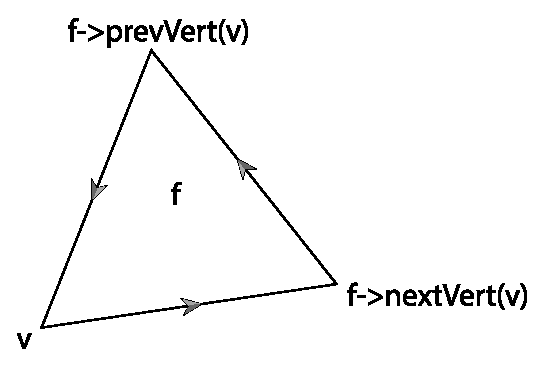
\includegraphics[width=0.35\linewidth]{chap03/Subdivprevnextvert.eps}
    \caption{给定顶点{\ttfamily v}和面{\ttfamily f},
    方法{\ttfamily f->\protect\refvar{prevVert}{}(v)}返回
    从{\ttfamily v}起绕该面的上一个顶点,
    而{\ttfamily f->\protect\refvar{nextVert}{}(v)}返回下一个顶点,
    其中“下一个”和“上一个”由定义该面时的顶点原始顺序定义。}
    \label{fig:3.31}
\end{figure}

\begin{lstlisting}
`\refcode{SDFace Methods}{+=}\lastnext{SDFaceMethods}`
`\refvar{SDVertex}{}` *`\initvar{nextVert}{}`(`\refvar{SDVertex}{}` *vert) {
    return `\refvar[SDFace::v]{v}{}`[`\refvar{NEXT}{}`(`\refvar{vnum}{}`(vert))];
}
\end{lstlisting}
\begin{lstlisting}
`\refcode{SDFace Methods}{+=}\lastnext{SDFaceMethods}`
`\refvar{SDVertex}{}` *`\initvar{prevVert}{}`(`\refvar{SDVertex}{}` *vert) {
    return `\refvar[SDFace::v]{v}{}`[`\refvar{PREV}{}`(`\refvar{vnum}{}`(vert))];
}
\end{lstlisting}

\subsection{细分}\label{sub:细分}
现在我们可以展示怎样用修改后的Loop规则进行细分了。

\section{控制舍入误差}\label{sec:控制舍入误差}

\begin{remark}
    本节含有高级内容,第一次阅读时可以跳过。
\end{remark}

到目前为止,我们都是根据基于实数的理想化算术运算
纯粹地讨论光线-形状相交算法。该方法已经让我们走得很远了,
尽管有个重要事实是计算机只能表示有限的数量,
因此它实际上不能表示所有实数。
计算机用浮点数代替实数,它有固定的存储要求。
然而,因为结果可能无法在特定量的内存中表示,
每执行一次浮点运算就可能引入误差。

该误差的累积对相交测试的精度有些许影响。
首先,它可能造成完全错过有效的相交——
例如,一个精确值是正数的相交处$t$值算成了负的。
而且,算得的光线-形状交点可能在形状实际曲面的上面或下面。
这导致一个问题:当从算得的交点开始为阴影射线和反射光线追踪新光线时,
若射线端点在实际曲面之下,我们可能求得一次与曲面错误的再相交。
反之,若端点在曲面上面离得太远,阴影和反射可能会脱钩(见\reffig{3.39})。
\begin{figure}[htbp]
    \centering%LaTeX with PSTricks extensions
%%Creator: Inkscape 1.0.1 (3bc2e813f5, 2020-09-07)
%%Please note this file requires PSTricks extensions
\psset{xunit=.45pt,yunit=.45pt,runit=.45pt}
\begin{pspicture}(384.51998901,248.1499939)
{
\newrgbcolor{curcolor}{0 0 0}
\pscustom[linewidth=1,linecolor=curcolor,linestyle=dashed,dash=2]
{
\newpath
\moveto(219.8500061,133.36999512)
\lineto(190.47000122,209.74999237)
}
}
{
\newrgbcolor{curcolor}{0 0 0}
\pscustom[linewidth=1,linecolor=curcolor]
{
\newpath
\moveto(236.88000488,89.4099884)
\lineto(220.97000122,130.44999695)
}
}
{
\newrgbcolor{curcolor}{0 0 0}
\pscustom[linestyle=none,fillstyle=solid,fillcolor=curcolor]
{
\newpath
\moveto(227.88,127.8599939)
\lineto(221.2,129.8399939)
\lineto(217.61,123.8799939)
\lineto(218.04,137.9999939)
\closepath
}
}
{
\newrgbcolor{curcolor}{0.65098041 0.65098041 0.65098041}
\pscustom[linestyle=none,fillstyle=solid,fillcolor=curcolor]
{
\newpath
\moveto(226.19,128.8799939)
\lineto(218.51,136.7799939)
\lineto(220.98,130.4299939)
\closepath
}
}
{
\newrgbcolor{curcolor}{0.40000001 0.40000001 0.40000001}
\pscustom[linestyle=none,fillstyle=solid,fillcolor=curcolor]
{
\newpath
\moveto(218.18,125.7699939)
\lineto(218.51,136.7799939)
\lineto(220.98,130.4299939)
\closepath
}
}
{
\newrgbcolor{curcolor}{0 0 0}
\pscustom[linewidth=1,linecolor=curcolor,linestyle=dashed,dash=2]
{
\newpath
\moveto(304.55,139.9099939)
\lineto(261.9,24.0399939)
\lineto(236.11,91.4999939)
}
}
{
\newrgbcolor{curcolor}{0 0 0}
\pscustom[linewidth=1,linecolor=curcolor]
{
\newpath
\moveto(320.82998657,184.15999222)
\lineto(307.3500061,147.51999664)
}
}
{
\newrgbcolor{curcolor}{0 0 0}
\pscustom[linestyle=none,fillstyle=solid,fillcolor=curcolor]
{
\newpath
\moveto(303.88,154.0299939)
\lineto(307.57,148.1299939)
\lineto(314.21,150.2299939)
\lineto(304.55,139.9099939)
\closepath
}
}
{
\newrgbcolor{curcolor}{0.65098041 0.65098041 0.65098041}
\pscustom[linestyle=none,fillstyle=solid,fillcolor=curcolor]
{
\newpath
\moveto(304.47,152.1499939)
\lineto(305,141.1499939)
\lineto(307.35,147.5399939)
\closepath
}
}
{
\newrgbcolor{curcolor}{0.40000001 0.40000001 0.40000001}
\pscustom[linestyle=none,fillstyle=solid,fillcolor=curcolor]
{
\newpath
\moveto(312.54,149.1799939)
\lineto(305,141.1499939)
\lineto(307.35,147.5399939)
\closepath
}
}
{
\newrgbcolor{curcolor}{0 0 0}
\pscustom[linewidth=1,linecolor=curcolor,linestyle=dashed,dash=2]
{
\newpath
\moveto(132.72999573,89.11999512)
\lineto(188.08999634,207.56999207)
}
}
{
\newrgbcolor{curcolor}{0 0 0}
\pscustom[linewidth=1,linecolor=curcolor]
{
\newpath
\moveto(110,40.87998962)
\lineto(129.27999878,81.78999329)
}
}
{
\newrgbcolor{curcolor}{0 0 0}
\pscustom[linestyle=none,fillstyle=solid,fillcolor=curcolor]
{
\newpath
\moveto(132.16,74.9999939)
\lineto(129,81.1999939)
\lineto(122.21,79.6899939)
\lineto(132.73,89.1199939)
\closepath
}
}
{
\newrgbcolor{curcolor}{0.65098041 0.65098041 0.65098041}
\pscustom[linestyle=none,fillstyle=solid,fillcolor=curcolor]
{
\newpath
\moveto(131.74,76.9199939)
\lineto(132.18,87.9299939)
\lineto(129.27,81.7699939)
\closepath
}
}
{
\newrgbcolor{curcolor}{0.40000001 0.40000001 0.40000001}
\pscustom[linestyle=none,fillstyle=solid,fillcolor=curcolor]
{
\newpath
\moveto(123.96,80.5899939)
\lineto(132.18,87.9299939)
\lineto(129.27,81.7699939)
\closepath
}
}
{
\newrgbcolor{curcolor}{0 0 0}
\pscustom[linewidth=1,linecolor=curcolor,linestyle=dashed,dash=2]
{
\newpath
\moveto(73.42,114.5799939)
\lineto(102.58,25.0299939)
\lineto(110,40.8699939)
}
}
{
\newrgbcolor{curcolor}{0 0 0}
\pscustom[linewidth=1,linecolor=curcolor]
{
\newpath
\moveto(58.33000183,160.93999481)
\lineto(70.91000366,122.28999329)
}
}
{
\newrgbcolor{curcolor}{0 0 0}
\pscustom[linestyle=none,fillstyle=solid,fillcolor=curcolor]
{
\newpath
\moveto(64.16,125.2499939)
\lineto(70.71,122.8999939)
\lineto(74.63,128.6599939)
\lineto(73.42,114.5799939)
\closepath
}
}
{
\newrgbcolor{curcolor}{0.65098041 0.65098041 0.65098041}
\pscustom[linestyle=none,fillstyle=solid,fillcolor=curcolor]
{
\newpath
\moveto(65.78,124.1399939)
\lineto(73.02,115.8299939)
\lineto(70.91,122.3099939)
\closepath
}
}
{
\newrgbcolor{curcolor}{0.40000001 0.40000001 0.40000001}
\pscustom[linestyle=none,fillstyle=solid,fillcolor=curcolor]
{
\newpath
\moveto(73.96,126.7999939)
\lineto(73.02,115.8299939)
\lineto(70.91,122.3099939)
\closepath
}
}
{
\newrgbcolor{curcolor}{0.98823529 0.93333334 0.12941177}
\pscustom[linestyle=none,fillstyle=solid,fillcolor=curcolor]
{
\newpath
\moveto(195.71,230.6399939)
\lineto(194.14,220.9699939)
\lineto(199.09,229.4199939)
\lineto(195.76,220.1999939)
\lineto(202.18,227.6099939)
\lineto(197.22,219.1599939)
\lineto(204.89,225.2599939)
\lineto(198.46,217.8599939)
\lineto(207.12,222.4499939)
\lineto(199.44,216.3599939)
\lineto(208.79,219.2699939)
\lineto(200.13,214.6999939)
\lineto(209.86,215.8499939)
\lineto(200.5,212.9499939)
\lineto(210.28,212.2899939)
\lineto(200.54,211.1599939)
\lineto(210.03,208.7099939)
\lineto(200.25,209.3899939)
\lineto(209.13,205.2399939)
\lineto(199.64,207.6999939)
\lineto(207.61,201.9899939)
\lineto(198.74,206.1499939)
\lineto(205.52,199.0699939)
\lineto(197.56,204.7999939)
\lineto(202.93,196.5999939)
\lineto(196.16,203.6799939)
\lineto(199.92,194.6299939)
\lineto(194.57,202.8499939)
\lineto(196.61,193.2599939)
\lineto(192.86,202.3099939)
\lineto(193.1,192.5199939)
\lineto(191.08,202.1099939)
\lineto(189.51,192.4299939)
\lineto(189.29,202.2299939)
\lineto(185.97,192.9999939)
\lineto(187.55,202.6799939)
\lineto(182.6,194.2199939)
\lineto(185.93,203.4399939)
\lineto(179.5,196.0299939)
\lineto(184.47,204.4899939)
\lineto(176.8,198.3899939)
\lineto(183.23,205.7799939)
\lineto(174.57,201.1999939)
\lineto(182.25,207.2799939)
\lineto(172.89,204.3699939)
\lineto(181.56,208.9399939)
\lineto(171.83,207.7899939)
\lineto(181.19,210.6899939)
\lineto(171.41,211.3599939)
\lineto(181.15,212.4899939)
\lineto(171.66,214.9299939)
\lineto(181.44,214.2599939)
\lineto(172.56,218.4099939)
\lineto(182.04,215.9399939)
\lineto(174.08,221.6599939)
\lineto(182.95,217.4899939)
\lineto(176.17,224.5699939)
\lineto(184.13,218.8499939)
\lineto(178.76,227.0499939)
\lineto(185.53,219.9599939)
\lineto(181.77,229.0099939)
\lineto(187.12,220.7999939)
\lineto(185.08,230.3799939)
\lineto(188.83,221.3299939)
\lineto(188.59,231.1299939)
\lineto(190.61,221.5399939)
\lineto(192.17,231.2099939)
\lineto(192.4,221.4199939)
\closepath
}
}
{
\newrgbcolor{curcolor}{0 0 0}
\pscustom[linewidth=0.30000001,linecolor=curcolor]
{
\newpath
\moveto(195.71,230.6399939)
\lineto(194.14,220.9699939)
\lineto(199.09,229.4199939)
\lineto(195.76,220.1999939)
\lineto(202.18,227.6099939)
\lineto(197.22,219.1599939)
\lineto(204.89,225.2599939)
\lineto(198.46,217.8599939)
\lineto(207.12,222.4499939)
\lineto(199.44,216.3599939)
\lineto(208.79,219.2699939)
\lineto(200.13,214.6999939)
\lineto(209.86,215.8499939)
\lineto(200.5,212.9499939)
\lineto(210.28,212.2899939)
\lineto(200.54,211.1599939)
\lineto(210.03,208.7099939)
\lineto(200.25,209.3899939)
\lineto(209.13,205.2399939)
\lineto(199.64,207.6999939)
\lineto(207.61,201.9899939)
\lineto(198.74,206.1499939)
\lineto(205.52,199.0699939)
\lineto(197.56,204.7999939)
\lineto(202.93,196.5999939)
\lineto(196.16,203.6799939)
\lineto(199.92,194.6299939)
\lineto(194.57,202.8499939)
\lineto(196.61,193.2599939)
\lineto(192.86,202.3099939)
\lineto(193.1,192.5199939)
\lineto(191.08,202.1099939)
\lineto(189.51,192.4299939)
\lineto(189.29,202.2299939)
\lineto(185.97,192.9999939)
\lineto(187.55,202.6799939)
\lineto(182.6,194.2199939)
\lineto(185.93,203.4399939)
\lineto(179.5,196.0299939)
\lineto(184.47,204.4899939)
\lineto(176.8,198.3899939)
\lineto(183.23,205.7799939)
\lineto(174.57,201.1999939)
\lineto(182.25,207.2799939)
\lineto(172.89,204.3699939)
\lineto(181.56,208.9399939)
\lineto(171.83,207.7899939)
\lineto(181.19,210.6899939)
\lineto(171.41,211.3599939)
\lineto(181.15,212.4899939)
\lineto(171.66,214.9299939)
\lineto(181.44,214.2599939)
\lineto(172.56,218.4099939)
\lineto(182.04,215.9399939)
\lineto(174.08,221.6599939)
\lineto(182.95,217.4899939)
\lineto(176.17,224.5699939)
\lineto(184.13,218.8499939)
\lineto(178.76,227.0499939)
\lineto(185.53,219.9599939)
\lineto(181.77,229.0099939)
\lineto(187.12,220.7999939)
\lineto(185.08,230.3799939)
\lineto(188.83,221.3299939)
\lineto(188.59,231.1299939)
\lineto(190.61,221.5399939)
\lineto(192.17,231.2099939)
\lineto(192.4,221.4199939)
\closepath
}
}
{
\newrgbcolor{curcolor}{0 0 0}
\pscustom[linewidth=1,linecolor=curcolor]
{
\newpath
\moveto(36.70000076,54.98999023)
\lineto(345.42999268,54.98999023)
}
}
{
\newrgbcolor{curcolor}{0 0 0}
\pscustom[linestyle=none,fillstyle=solid,fillcolor=curcolor]
{
\newpath
\moveto(104.71000051,25.27999878)
\curveto(104.71000051,27.3737707)(102.17872502,28.4219561)(100.69838415,26.94161524)
\curveto(99.21804329,25.46127437)(100.26622869,22.92999887)(102.36000061,22.92999887)
\curveto(104.45377253,22.92999887)(105.50195793,25.46127437)(104.02161707,26.94161524)
\curveto(102.5412762,28.4219561)(100.01000071,27.3737707)(100.01000071,25.27999878)
\curveto(100.01000071,23.18622686)(102.5412762,22.13804146)(104.02161707,23.61838232)
\curveto(105.50195793,25.09872318)(104.45377253,27.62999868)(102.36000061,27.62999868)
\curveto(100.26622869,27.62999868)(99.21804329,25.09872318)(100.69838415,23.61838232)
\curveto(102.17872502,22.13804146)(104.71000051,23.18622686)(104.71000051,25.27999878)
\closepath
}
}
{
\newrgbcolor{curcolor}{0 0 0}
\pscustom[linewidth=1,linecolor=curcolor]
{
\newpath
\moveto(104.71000051,25.27999878)
\curveto(104.71000051,27.3737707)(102.17872502,28.4219561)(100.69838415,26.94161524)
\curveto(99.21804329,25.46127437)(100.26622869,22.92999887)(102.36000061,22.92999887)
\curveto(104.45377253,22.92999887)(105.50195793,25.46127437)(104.02161707,26.94161524)
\curveto(102.5412762,28.4219561)(100.01000071,27.3737707)(100.01000071,25.27999878)
\curveto(100.01000071,23.18622686)(102.5412762,22.13804146)(104.02161707,23.61838232)
\curveto(105.50195793,25.09872318)(104.45377253,27.62999868)(102.36000061,27.62999868)
\curveto(100.26622869,27.62999868)(99.21804329,25.09872318)(100.69838415,23.61838232)
\curveto(102.17872502,22.13804146)(104.71000051,23.18622686)(104.71000051,25.27999878)
\closepath
}
}
{
\newrgbcolor{curcolor}{0 0 0}
\pscustom[linestyle=none,fillstyle=solid,fillcolor=curcolor]
{
\newpath
\moveto(264.26000357,25.27999878)
\curveto(264.26000357,27.3737707)(261.72872807,28.4219561)(260.24838721,26.94161524)
\curveto(258.76804634,25.46127437)(259.81623174,22.92999887)(261.91000366,22.92999887)
\curveto(264.00377558,22.92999887)(265.05196098,25.46127437)(263.57162012,26.94161524)
\curveto(262.09127926,28.4219561)(259.56000376,27.3737707)(259.56000376,25.27999878)
\curveto(259.56000376,23.18622686)(262.09127926,22.13804146)(263.57162012,23.61838232)
\curveto(265.05196098,25.09872318)(264.00377558,27.62999868)(261.91000366,27.62999868)
\curveto(259.81623174,27.62999868)(258.76804634,25.09872318)(260.24838721,23.61838232)
\curveto(261.72872807,22.13804146)(264.26000357,23.18622686)(264.26000357,25.27999878)
\closepath
}
}
{
\newrgbcolor{curcolor}{0 0 0}
\pscustom[linewidth=1,linecolor=curcolor]
{
\newpath
\moveto(264.26000357,25.27999878)
\curveto(264.26000357,27.3737707)(261.72872807,28.4219561)(260.24838721,26.94161524)
\curveto(258.76804634,25.46127437)(259.81623174,22.92999887)(261.91000366,22.92999887)
\curveto(264.00377558,22.92999887)(265.05196098,25.46127437)(263.57162012,26.94161524)
\curveto(262.09127926,28.4219561)(259.56000376,27.3737707)(259.56000376,25.27999878)
\curveto(259.56000376,23.18622686)(262.09127926,22.13804146)(263.57162012,23.61838232)
\curveto(265.05196098,25.09872318)(264.00377558,27.62999868)(261.91000366,27.62999868)
\curveto(259.81623174,27.62999868)(258.76804634,25.09872318)(260.24838721,23.61838232)
\curveto(261.72872807,22.13804146)(264.26000357,23.18622686)(264.26000357,25.27999878)
\closepath
}
}
{
\newrgbcolor{curcolor}{0 0 0}
\pscustom[linewidth=1,linecolor=curcolor]
{
\newpath
\moveto(225.3999939,66.95999146)
\lineto(258.75,85.07998657)
}
}
{
\newrgbcolor{curcolor}{1 1 1}
\pscustom[linestyle=none,fillstyle=solid,fillcolor=curcolor]
{
\newpath
\moveto(111.72000265,38.94999695)
\curveto(111.72000265,41.04376887)(109.18872715,42.09195427)(107.70838629,40.6116134)
\curveto(106.22804543,39.13127254)(107.27623082,36.59999704)(109.37000275,36.59999704)
\curveto(111.46377467,36.59999704)(112.51196006,39.13127254)(111.0316192,40.6116134)
\curveto(109.55127834,42.09195427)(107.02000284,41.04376887)(107.02000284,38.94999695)
\curveto(107.02000284,36.85622503)(109.55127834,35.80803963)(111.0316192,37.28838049)
\curveto(112.51196006,38.76872135)(111.46377467,41.29999685)(109.37000275,41.29999685)
\curveto(107.27623082,41.29999685)(106.22804543,38.76872135)(107.70838629,37.28838049)
\curveto(109.18872715,35.80803963)(111.72000265,36.85622503)(111.72000265,38.94999695)
\closepath
}
}
{
\newrgbcolor{curcolor}{0 0 0}
\pscustom[linewidth=1,linecolor=curcolor]
{
\newpath
\moveto(111.72000265,38.94999695)
\curveto(111.72000265,41.04376887)(109.18872715,42.09195427)(107.70838629,40.6116134)
\curveto(106.22804543,39.13127254)(107.27623082,36.59999704)(109.37000275,36.59999704)
\curveto(111.46377467,36.59999704)(112.51196006,39.13127254)(111.0316192,40.6116134)
\curveto(109.55127834,42.09195427)(107.02000284,41.04376887)(107.02000284,38.94999695)
\curveto(107.02000284,36.85622503)(109.55127834,35.80803963)(111.0316192,37.28838049)
\curveto(112.51196006,38.76872135)(111.46377467,41.29999685)(109.37000275,41.29999685)
\curveto(107.27623082,41.29999685)(106.22804543,38.76872135)(107.70838629,37.28838049)
\curveto(109.18872715,35.80803963)(111.72000265,36.85622503)(111.72000265,38.94999695)
\closepath
}
}
{
\newrgbcolor{curcolor}{1 1 1}
\pscustom[linestyle=none,fillstyle=solid,fillcolor=curcolor]
{
\newpath
\moveto(240.07000113,87.34999084)
\curveto(240.07000113,89.44376277)(237.53872563,90.49194816)(236.05838476,89.0116073)
\curveto(234.5780439,87.53126644)(235.6262293,84.99999094)(237.72000122,84.99999094)
\curveto(239.81377314,84.99999094)(240.86195854,87.53126644)(239.38161768,89.0116073)
\curveto(237.90127682,90.49194816)(235.37000132,89.44376277)(235.37000132,87.34999084)
\curveto(235.37000132,85.25621892)(237.90127682,84.20803353)(239.38161768,85.68837439)
\curveto(240.86195854,87.16871525)(239.81377314,89.69999075)(237.72000122,89.69999075)
\curveto(235.6262293,89.69999075)(234.5780439,87.16871525)(236.05838476,85.68837439)
\curveto(237.53872563,84.20803353)(240.07000113,85.25621892)(240.07000113,87.34999084)
\closepath
}
}
{
\newrgbcolor{curcolor}{0 0 0}
\pscustom[linewidth=1,linecolor=curcolor]
{
\newpath
\moveto(240.07000113,87.34999084)
\curveto(240.07000113,89.44376277)(237.53872563,90.49194816)(236.05838476,89.0116073)
\curveto(234.5780439,87.53126644)(235.6262293,84.99999094)(237.72000122,84.99999094)
\curveto(239.81377314,84.99999094)(240.86195854,87.53126644)(239.38161768,89.0116073)
\curveto(237.90127682,90.49194816)(235.37000132,89.44376277)(235.37000132,87.34999084)
\curveto(235.37000132,85.25621892)(237.90127682,84.20803353)(239.38161768,85.68837439)
\curveto(240.86195854,87.16871525)(239.81377314,89.69999075)(237.72000122,89.69999075)
\curveto(235.6262293,89.69999075)(234.5780439,87.16871525)(236.05838476,85.68837439)
\curveto(237.53872563,84.20803353)(240.07000113,85.25621892)(240.07000113,87.34999084)
\closepath
}
}
\end{pspicture}

    \caption{可能在图像中造成可见错误的舍入误差问题几何设置。
        左边的入射光线与曲面相交。在左图中,算得的交点(黑圆圈)略低于曲面
        且阴影射线端点过低的“epsilon”偏移可能导致错误的自相交,
        因为阴影射线端点(白圆圈)仍在曲面之下;因此错误地认定光源被遮挡了。
        右图中,太高的“epsilon”导致错过了有效相交,
        因为射线端点通过了遮挡面。}
    \label{fig:3.39}
\end{figure}

在光线追踪中解决该问题的典型实践是将生成的射线偏移固定的“射线epsilon”值
\sidenote{译者注:epsilon即希腊字母$\epsilon$。},
忽略沿射线$\bm p+t\bm d$比某个$t_{\min}$还近的任何相交。
\reffig{3.40}展示了为什么该方法需要很高的$t_{\min}$值才能高效工作:
如果生成的射线相对于曲面非常倾斜,
则在离射线很远处可能会发生错误的射线相交。
不幸的是,大的$t_{\min}$值会造成射线端点相对远离原始交点,
这又反过来造成错过附近的有效相交,导致阴影和反射丢失细节。
\begin{figure}[htbp]
    \centering%LaTeX with PSTricks extensions
%%Creator: Inkscape 1.0.1 (3bc2e813f5, 2020-09-07)
%%Please note this file requires PSTricks extensions
\psset{xunit=.5pt,yunit=.5pt,runit=.5pt}
\begin{pspicture}(311.58999634,120.58000183)
{
\newrgbcolor{curcolor}{0 0 0}
\pscustom[linewidth=1,linecolor=curcolor]
{
\newpath
\moveto(0,32.56000519)
\lineto(308.73001099,32.56000519)
}
}
{
\newrgbcolor{curcolor}{0 0 0}
\pscustom[linestyle=none,fillstyle=solid,fillcolor=curcolor]
{
\newpath
\moveto(68.00000143,2.84999847)
\curveto(68.00000143,4.9437704)(65.46872593,5.99195579)(63.98838507,4.51161493)
\curveto(62.50804421,3.03127407)(63.5562296,0.49999857)(65.65000153,0.49999857)
\curveto(67.74377345,0.49999857)(68.79195884,3.03127407)(67.31161798,4.51161493)
\curveto(65.83127712,5.99195579)(63.30000162,4.9437704)(63.30000162,2.84999847)
\curveto(63.30000162,0.75622655)(65.83127712,-0.29195884)(67.31161798,1.18838202)
\curveto(68.79195884,2.66872288)(67.74377345,5.19999838)(65.65000153,5.19999838)
\curveto(63.5562296,5.19999838)(62.50804421,2.66872288)(63.98838507,1.18838202)
\curveto(65.46872593,-0.29195884)(68.00000143,0.75622655)(68.00000143,2.84999847)
\closepath
}
}
{
\newrgbcolor{curcolor}{0 0 0}
\pscustom[linewidth=1,linecolor=curcolor]
{
\newpath
\moveto(68.00000143,2.84999847)
\curveto(68.00000143,4.9437704)(65.46872593,5.99195579)(63.98838507,4.51161493)
\curveto(62.50804421,3.03127407)(63.5562296,0.49999857)(65.65000153,0.49999857)
\curveto(67.74377345,0.49999857)(68.79195884,3.03127407)(67.31161798,4.51161493)
\curveto(65.83127712,5.99195579)(63.30000162,4.9437704)(63.30000162,2.84999847)
\curveto(63.30000162,0.75622655)(65.83127712,-0.29195884)(67.31161798,1.18838202)
\curveto(68.79195884,2.66872288)(67.74377345,5.19999838)(65.65000153,5.19999838)
\curveto(63.5562296,5.19999838)(62.50804421,2.66872288)(63.98838507,1.18838202)
\curveto(65.46872593,-0.29195884)(68.00000143,0.75622655)(68.00000143,2.84999847)
\closepath
}
}
{
\newrgbcolor{curcolor}{0 0 0}
\pscustom[linewidth=1,linecolor=curcolor,linestyle=dashed,dash=2]
{
\newpath
\moveto(129.72999573,15.99000549)
\lineto(311.48999023,53.27999878)
}
}
{
\newrgbcolor{curcolor}{0 0 0}
\pscustom[linewidth=1,linecolor=curcolor,linestyle=dashed,dash=2]
{
\newpath
\moveto(120.30999756,14.06000519)
\lineto(129.72999573,15.99000549)
}
}
{
\newrgbcolor{curcolor}{0 0 0}
\pscustom[linewidth=1,linecolor=curcolor]
{
\newpath
\moveto(65.65000153,2.84999847)
\lineto(112.37999725,12.43000031)
}
}
{
\newrgbcolor{curcolor}{0 0 0}
\pscustom[linestyle=none,fillstyle=solid,fillcolor=curcolor]
{
\newpath
\moveto(108.67,6.05000183)
\lineto(111.74,12.30000183)
\lineto(106.46,16.84000183)
\lineto(120.31,14.06000183)
\closepath
}
}
{
\newrgbcolor{curcolor}{0.65098041 0.65098041 0.65098041}
\pscustom[linestyle=none,fillstyle=solid,fillcolor=curcolor]
{
\newpath
\moveto(109.96,7.55000183)
\lineto(119.03,13.80000183)
\lineto(112.36,12.43000183)
\closepath
}
}
{
\newrgbcolor{curcolor}{0.40000001 0.40000001 0.40000001}
\pscustom[linestyle=none,fillstyle=solid,fillcolor=curcolor]
{
\newpath
\moveto(108.23,15.97000183)
\lineto(119.03,13.80000183)
\lineto(112.36,12.43000183)
\closepath
}
}
{
\newrgbcolor{curcolor}{0 0 0}
\pscustom[linewidth=1,linecolor=curcolor,linestyle=dashed,dash=2]
{
\newpath
\moveto(43.90000153,75.87000275)
\lineto(65.65000153,2.84999847)
}
}
{
\newrgbcolor{curcolor}{0 0 0}
\pscustom[linewidth=1,linecolor=curcolor]
{
\newpath
\moveto(30.62000084,120.44000183)
\lineto(41.58000183,83.6400032)
}
}
{
\newrgbcolor{curcolor}{0 0 0}
\pscustom[linestyle=none,fillstyle=solid,fillcolor=curcolor]
{
\newpath
\moveto(34.91,86.77000183)
\lineto(41.4,84.26000183)
\lineto(45.46,89.92000183)
\lineto(43.9,75.87000183)
\closepath
}
}
{
\newrgbcolor{curcolor}{0.65098041 0.65098041 0.65098041}
\pscustom[linestyle=none,fillstyle=solid,fillcolor=curcolor]
{
\newpath
\moveto(36.5,85.62000183)
\lineto(43.52,77.13000183)
\lineto(41.58,83.66000183)
\closepath
}
}
{
\newrgbcolor{curcolor}{0.40000001 0.40000001 0.40000001}
\pscustom[linestyle=none,fillstyle=solid,fillcolor=curcolor]
{
\newpath
\moveto(44.74,88.08000183)
\lineto(43.52,77.13000183)
\lineto(41.58,83.66000183)
\closepath
}
}
{
\newrgbcolor{curcolor}{1 1 1}
\pscustom[linestyle=none,fillstyle=solid,fillcolor=curcolor]
{
\newpath
\moveto(212.12000418,32.54000092)
\curveto(212.12000418,34.63377284)(209.58872868,35.68195823)(208.10838782,34.20161737)
\curveto(206.62804695,32.72127651)(207.67623235,30.19000101)(209.77000427,30.19000101)
\curveto(211.8637762,30.19000101)(212.91196159,32.72127651)(211.43162073,34.20161737)
\curveto(209.95127987,35.68195823)(207.42000437,34.63377284)(207.42000437,32.54000092)
\curveto(207.42000437,30.44622899)(209.95127987,29.3980436)(211.43162073,30.87838446)
\curveto(212.91196159,32.35872532)(211.8637762,34.89000082)(209.77000427,34.89000082)
\curveto(207.67623235,34.89000082)(206.62804695,32.35872532)(208.10838782,30.87838446)
\curveto(209.58872868,29.3980436)(212.12000418,30.44622899)(212.12000418,32.54000092)
\closepath
}
}
{
\newrgbcolor{curcolor}{0 0 0}
\pscustom[linewidth=1,linecolor=curcolor]
{
\newpath
\moveto(212.12000418,32.54000092)
\curveto(212.12000418,34.63377284)(209.58872868,35.68195823)(208.10838782,34.20161737)
\curveto(206.62804695,32.72127651)(207.67623235,30.19000101)(209.77000427,30.19000101)
\curveto(211.8637762,30.19000101)(212.91196159,32.72127651)(211.43162073,34.20161737)
\curveto(209.95127987,35.68195823)(207.42000437,34.63377284)(207.42000437,32.54000092)
\curveto(207.42000437,30.44622899)(209.95127987,29.3980436)(211.43162073,30.87838446)
\curveto(212.91196159,32.35872532)(211.8637762,34.89000082)(209.77000427,34.89000082)
\curveto(207.67623235,34.89000082)(206.62804695,32.35872532)(208.10838782,30.87838446)
\curveto(209.58872868,29.3980436)(212.12000418,30.44622899)(212.12000418,32.54000092)
\closepath
}
}
\end{pspicture}

    \caption{如果算得的交点(实心圆)低于曲面且生成的射线是斜的,
        在与射线端点有一定距离的地方可能会发生错误的再相交(空心圆)。
        如果用沿射线的最小$t$值消除附近的相交,
        需要相对大的$t_{\min}$才能处理好倾斜射线。}
    \label{fig:3.40}
\end{figure}

本节中,我们将介绍浮点算术基本思想并描述分析浮点计算误差的技术。
然后我们将这些方法用于本章之前介绍的光线-形状算法
并展示怎样计算带有有界误差的光线交点。
这将允许我们保守地定位射线端点,这样就永远不会求得错误的自相交,
而又保留了与实际交点极其接近的射线端点使得错误脱靶被最小化。
反过来也不需要额外的“射线epsilon”值。

\subsection{浮点算术}\label{sub:浮点算术}
计算必须在容纳于有限量内存的数字的有限表示上执行;
计算机上无法表示实数的无限集合。
一种这样的有限表示是定点,例如给定一个16位整数,
有人可能通过除以256将其映射为正实数。
这允许我们表示值之间具有相等间距$\displaystyle\frac{1}{256}$的
范围$\displaystyle\left[0,\frac{65535}{256}\right]=\left[0,255+\frac{255}{256}\right]$。
\keyindex{定点数}{fixed-point number}{}可以用整数算术运算高效实现
(该特性使其在早期不支持浮点计算的个人计算机上很流行),
但是它们受制于许多缺点:其中,它们能表示的最大数字是受限的,
且不能精确表示非常小的接近于零的数。

计算机上实数的另一种表示是\keyindex{浮点数}{floating-point number}{}。
它用\keyindex{符号}{sign}{}、\keyindex{有效数字}{significand}{}\footnote{单词“\protect\keyindex{尾数}{mantissa}{}”
    常用来代替“有效数字”,但浮点纯粹主义者注意到“尾数”在对数上下文中
    有不同含义而因此更偏爱“有效数字”。这里我们遵循该用法。}和\keyindex{指数}{exponent}{}表示数字:
本质上和\keyindex{科学计数法}{scientific notation}{}相同但用固定数量的数字表示有效数字和指数。
(下文中,我们将只讨论以2为底的数字。)
这种表示能够用固定数量的存储对极大范围的数字进行表示和执行计算。

用浮点算术的程序员通常知道浮点是不精确的;
有时这种看法导致了浮点算术是不可预测的观念。
本节中我们将看到浮点算术有精心设计的基础反而
能计算特定计算中引入误差的保守边界。
对于光线追踪计算,该误差常意外地小。

现代CPU和GPU几乎都基于电气与电子工程师协会
\sidenote{译者注:即Institute of Electrical and Electronics Engineers (IEEE),
    是电气工程与电子工程以及相关学科的专业协会,成立于1963年1月,总部在美国纽约。
    其范围已经扩展到电气、电子、通信、计算机工程、计算机科学与信息技术等诸多领域,
    是世界上最大的技术专业组织。}
颁布的标准\parencite*{10.1109/IEEESTD.1985.82928,10.1109/IEEESTD.2008.4610935}实现浮点算术模型。
(今后我们说的浮点特指IEEE 754规定的32位浮点数。)
IEEE 754技术标准规定了内存中浮点数的格式以及
精度和浮点计算舍入的特定规则;
正是这些规则使得能对给定浮点值中出现的误差进行严格推导。

\subsubsection*{浮点表示}
IEEE标准规定32位浮点用1位符号、8位指数和23位有效数字表示。
用了8位的指数$e$范围为从0到255;
实际用的指数$e_{\mathrm{b}}$是通过偏置$e$算得的:
\begin{align*}
    e_{\mathrm{b}}=e-127\, .
\end{align*}

当存储\keyindex{规范化的}{normalized}{}浮点值时有效数字实际有24位精度。
当有效数字和指数表示规范化的数字时,有效数字中没有前导零。
在\keyindex{二进制}{binary}{}中,这意味着有效数字开头的数字必须是一;
反过来,没必要显式存储该值。
因此,隐式前导的1位和编码有效数字小数部分的23位给出了总共24位的精度。

给定符号$s=\pm 1$、有效数字$m$和指数$e$,相应的浮点值为
\begin{align*}
    s\times 1.m\times2^{e-127}\, .
\end{align*}

例如,浮点数6.5可以通过规范化的有效数字写作$1.101_2\times2^2$,
其中下标2表示以2为底的值\sidenote{译者注:即二进制。}
(如果非整数的二进制数不够直观,可以注意
小数点右边第一个数表示$2^{-1}$,以此类推)。
因此,我们有
\begin{align*}
    (1\times2^0+1\times2^{-1}+0\times2^{-2}+1\times2^{-3})\times2^2=1.625\times2^2=6.5\, .
\end{align*}
$e_{\mathrm{b}}=2$,所以$e=129=10000001_2$且$m=10100000000000000000000_2$。

浮点在内存中的布局是符号位在32位值的最高位
(负号用一位编码),然后是指数和有效数字。
因此,对于值6.5其内存中的二进制表示是
\begin{align*}
    0\ 10000001\ 10100000000000000000000=40\mathrm{d}00000_{16}\, .
\end{align*}

同样,浮点值1.0有$m=0\ldots0_2$和$e_{\mathrm{b}}=0$,所以$e=127=01111111_2$,它的二进制表示为
\begin{align*}
    0\ 01111111\ 00000000000000000000000=3\mathrm{f}800000_{16}\, .
\end{align*}

该\keyindex{十六进制}{hexadecimal}{}值值得记住,因为调试时它常出现于内存转储。

该表示隐含了整个范围内两个相邻的二的幂次之间
可表示的浮点数之间的间隔是均匀的(它对应于有效数字位增一)。
在范围$[2^e,2^{e+1})$内,间隔为
\begin{align}\label{eq:3.6}
    2^{e-23}\, .
\end{align}
因此对1和2之间的浮点数,$e=0$,
浮点值间的间隔为$2^{-23}\approx1.19209\times10^{-7}$。
该间隔也称为\keyindex{最后一位上的单位值}{unit in last place}{}(ulp)\sidenote{译者注:也叫“最小精度单位”。}的大小;
注意一个ulp的大小由相应浮点值决定——更大的数的ulp比更小的数的ulp相对更大。

按我们目前描述的表示是不可能恰好将零表示为浮点数的。
这事显然不可接受,所以最小指数$e=0$,
或说$e_{\mathrm{b}}=-127$,被留出来特殊对待。
对于该指数,浮点值解释为有效数字中没有隐式前导一位,
这意味全零位的有效数字会得到
\begin{align*}
    s\times0.0\ldots0_2\times2^{-127}=0\, .
\end{align*}

去掉有效数字前导一位也能表示\keyindex{非规范化的}{denormalized}{}数:
如果总是出现前导一\sidenote{译者注:我完善了该式。},则最小的32位浮点是
\begin{align*}
    1.{\underbrace{0\ldots0}_{\text{23个0}}}\ _2\times2^{-127}\approx5.8774718\times10^{-39}\, .
\end{align*}
没有前导一位\sidenote{译者注:我完善了该式;如果你难以理解为何指数变成了$2^{-126}$,
也可以等价地看作$\underbrace{0.0\ldots0}_{22\text{个}0}1_2\times2^{-127}=2^{-22}\times2^{-127}$。},最小值是
\begin{align*}
    0.\underbrace{0\ldots0}_{\text{22个0}}1_2\times2^{-126}=2^{-23}\times2^{-126}\approx1.4012985\times10^{-45}\, .
\end{align*}

有了表示这些小值的能力可以避免需要将非常小的数舍入为零。

注意该表示同时有“正”和“负”零值。
该细节对程序员大多是透明的。
例如,标准保证了比较{\ttfamily -0.0 == 0.0}为真,
即使这两值在内存中的表示不同。

最大指数,$e=255$,也保留作特殊对待。
因此,可以表示的最大规范化浮点值有$e=254$(或$e_{\mathrm{b}}=127$)且约为\sidenote{译者注:我完善了该式。}
\begin{align*}
    1.{\underbrace{1\ldots1}_{\text{23个1}}}\ _2\times2^{127}=(2-2^{-23})\times2^{127}\approx3.402823\times10^{38}\, .
\end{align*}

对于$e=255$,若有效数字位全是零,则该值依据符号位对应正或负无穷。
例如,在浮点中执行像1/0的计算会得到无穷值。
对无穷的算术运算得到无穷。
比较时,正无穷大于任何非无穷值,负无穷类似。

常数\refvar{MaxFloat}{}和\refvar{Infinity}{}分别初始化为可表示的最大和“无穷”浮点值。
我们令其可在单独的常数中获取,这样使用这些值的代码
就不需要用唠叨的C++标准库调用来获取它们的值了。
\begin{lstlisting}
`\initcode{Global Constants}{=}\initnext{GlobalConstants}`
static constexpr `\refvar{Float}{}` `\initvar{MaxFloat}{}` = std::numeric_limits<`\refvar{Float}{}`>::max();
static constexpr `\refvar{Float}{}` `\initvar{Infinity}{}` = std::numeric_limits<`\refvar{Float}{}`>::infinity();
\end{lstlisting}

对于$e=255$,非零有效数字位对应
特殊的NaN值\sidenote{译者注:原文误写为$e_b=255$,已修正。},
它由诸如取负数平方根或尝试计算0/0的运算得到。
NaN随计算传播:\keyindex{运算对象}{operand}{}之一
为NaN本身的任何算术运算总是返回NaN。
因此,如果NaN出现于一长串计算中,
我们就知道该方式中的某处出错了。
在调试构建中,pbrt有许多\refvar{Assert}{()}语句检查NaN值,
因为我们几乎从不希望它们出现在事件的常规过程中。
任何与NaN值的比较返回假;
因此检查{\ttfamily !(x == x)}用来检查值是否不是数字
\footnote{这是编译器不得对包含浮点值的表达式执行
看似明显且安全的代数简化的少数几个地方之一——
这个特别的比较不得简化为{\ttfamily false}。
启用编译器的“快速数学”或“执行不安全的数学优化”标志
可能会允许执行这些优化。但是错误行为可能引入pbrt中。}。
为了清楚起见,我们用C++标准库函数{\ttfamily std::isnan()}来检查NaN值。

\subsubsection*{实用例程}
对于某些底层运算,能将浮点值解释为其组成位以及将表示浮点值的数位
转换为实际的{\ttfamily float}或{\ttfamily double}很有用。

一个自然的方法是取指向要转换的值的指针并将其强制转换为另一类型:
{\ttfamily\newline\noindent
float f = ...;\newline\noindent
uint32\_t bits = *((uint32\_t *)\&f);\newline
}
然而,现代版本的C++规定将一种{\ttfamily float}指针强制转换为
不同类型{\ttfamily uint32\_t}是非法的
(该限制允许编译器在分析两个指针是否可能指向
同一内存位置时进行更激进的优化,禁止在寄存器中保存值)。

另一常见方法是对两类元素使用{\ttfamily union},赋予一种类型并按另一种读取:
{\ttfamily\newline\noindent
union FloatBits \{\newline\noindent
\indent float f;\newline\noindent
\indent uint32\_t ui;\newline\noindent
\};\newline\noindent
FloatBits fb;\newline\noindent
fb.f = ...;\newline\noindent
uint32\_t bits = fb.ui;
}

这也是非法的:C++标准说从{\ttfamily union}读取和最后一次赋值时不同的元素是未定义行为。

可以用{\ttfamily memcpy()}将指向源类型的指针复制到指向目标类型的指针来正确执行这些转换。
\begin{lstlisting}
`\initcode{Global Inline Functions}{=}\initnext{GlobalInlineFunctions}`
inline uint32_t `\initvar{FloatToBits}{}`(float f) {
    uint32_t ui;
    memcpy(&ui, &f, sizeof(float));
    return ui;
}
\end{lstlisting}
\begin{lstlisting}
`\refcode{Global Inline Functions}{+=}\lastnext{GlobalInlineFunctions}`
inline float `\initvar{BitsToFloat}{}`(uint32_t ui) {
    float f;
    memcpy(&f, &ui, sizeof(uint32_t));
    return f;
}
\end{lstlisting}

尽管调用函数{\ttfamily memcpy()}以避免这些问题可能看起来太昂贵了,
但实际中好的编译器会将其变为无操作而只是将寄存器或内存中的内容重新解释为另一类型
(pbrt中还有这些函数在{\ttfamily double}和{\ttfamily uint64\_t}之间
转换的类似版本,所以这里就不介绍了)。

这些转换可用于实现函数即把浮点值向上或向下调整到相邻更大或更小的可表示浮点值
\footnote{这些函数等价于{\ttfamily std::nextafter(v, Infinity)}和{\ttfamily std::nextafter(v, -Infinity)}但更加高效,
因为它们不负责处理NaN值或浮点信号异常。}。
它们对我们接下来的代码中需要的某些保守的舍入操作很有用。
多亏浮点在内存中表示的特殊性,这些操作很高效。
\begin{lstlisting}
`\refcode{Global Inline Functions}{+=}\lastnext{GlobalInlineFunctions}`
inline float `\initvar{NextFloatUp}{}`(float v) {
    `\refcode{Handle infinity and negative zero for NextFloatUp()}{}`
    `\refcode{Advance v to next higher float}{}`
}
\end{lstlisting}

有两种重要的特殊情况:如果{\ttfamily v}为正无穷,则该函数就返回没变的{\ttfamily v}。
在继续执行有效数字的代码之前让负零向前跳到正零。
这一步必须显式处理,因为-0.0和0.0的位模式不相邻。
\begin{lstlisting}
`\initcode{Handle infinity and negative zero for NextFloatUp()}{=}`
if (std::isinf(v) && v > 0.)
    return v;
if (v == -0.f)
    v = 0.f;
\end{lstlisting}

概念上,给定一浮点值,我们想对有效数字增加一,
如果结果\keyindex{溢出}{overflow}{},
则有效数字重置为零且指数增加一。
意外的是对浮点在内存中的整数表示加一实现了这点:
因为指数在有效数字之上的高位,所以如果有效数字全是一,
则有效数字低位加一会将一一路带到指数去,
否则就在当前指数下推进到相邻更大的有效数字。
还要注意当增加最大可表示的有限浮点值数位表示时,
会得到正的浮点无穷数位模式。

对于负值,从数位表示减一类似地推进到相邻值。
\begin{lstlisting}
`\initcode{Advance v to next higher float}{=}`
uint32_t ui = `\refvar{FloatToBits}{}`(v);
if (v >= 0) ++ui;
else        --ui;
return `\refvar{BitsToFloat}{}`(ui);
\end{lstlisting}

这里没有介绍函数{\initvar{NextFloatDown}{()}}了,
它遵循相同的逻辑但高效地取反。
pbrt也提供了这些函数的{\ttfamily double}版本。

\subsubsection*{算术运算}
IEEE 754提供了关于浮点算术的重要保证:
具体而言,它保证了加法、减法、乘法、除法和平方根
在相同输入下给出相同结果且这些结果的浮点数最接近于
在无限精度算术下执行底层计算的结果
\footnote{IEEE浮点允许用户选一种数字舍入模式,
    但我们这里假设用默认的——舍入到最近的偶数。}。
值得注意的是这在有限精度数字计算机上是完全可能的;
IEEE 754的成就之一是证明了这种级别的精度是可能的且
能在硬件上很高效地实现。

用圆圈运算符表示浮点算术运算符,用sqrt表示浮点平方根,
这些精度保证可以写作:
\begin{align}
    a\oplus b        & =\mathrm{round}(a+b)\, ,\nonumber      \\
    a\ominus b       & =\mathrm{round}(a-b)\, ,\nonumber      \\
    a\otimes b       & =\mathrm{round}(a*b)\, ,\label{eq:3.7} \\
    a\oslash b       & =\mathrm{round}(a/b)\, ,\nonumber      \\
    \mathrm{sqrt}(a) & =\mathrm{round}(\sqrt{a})\, ,\nonumber
\end{align}
其中$\mathrm{round}(x)$表示将实数舍入到最接近的浮点值的结果。

舍入误差的界可以表示为实数区间:例如
对于加法,我们可以说舍入的结果在与某个$\epsilon$有关的区间内
\begin{align}
    a\oplus b & =\mathrm{round}(a+b)\in(a+b)(1\pm\epsilon)\nonumber \\
              & =[(a+b)(1-\epsilon),(a+b)(1+\epsilon)]\, ,
    \label{eq:3.8}
\end{align}
该舍入引入的误差量不超过在$a+b$处的浮点间隔的一半——
如果它超过浮点间隔的一半,则它会以更小误差舍入到另一个不同的浮点数(\reffig{3.41})。
\begin{figure}[htbp]
    \centering%LaTeX with PSTricks extensions
%%Creator: Inkscape 1.0.1 (3bc2e813f5, 2020-09-07)
%%Please note this file requires PSTricks extensions
\psset{xunit=.5pt,yunit=.5pt,runit=.5pt}
\begin{pspicture}(290.97000122,48.74321747)
{
\newrgbcolor{curcolor}{0 0 0}
\pscustom[linestyle=none,fillstyle=solid,fillcolor=curcolor]
{
\newpath
\moveto(175.22998953,38.20321655)
\curveto(175.22998953,40.29698848)(172.69871403,41.34517387)(171.21837317,39.86483301)
\curveto(169.73803231,38.38449215)(170.7862177,35.85321665)(172.87998962,35.85321665)
\curveto(174.97376155,35.85321665)(176.02194694,38.38449215)(174.54160608,39.86483301)
\curveto(173.06126522,41.34517387)(170.52998972,40.29698848)(170.52998972,38.20321655)
\curveto(170.52998972,36.10944463)(173.06126522,35.06125923)(174.54160608,36.5416001)
\curveto(176.02194694,38.02194096)(174.97376155,40.55321646)(172.87998962,40.55321646)
\curveto(170.7862177,40.55321646)(169.73803231,38.02194096)(171.21837317,36.5416001)
\curveto(172.69871403,35.06125923)(175.22998953,36.10944463)(175.22998953,38.20321655)
\closepath
}
}
{
\newrgbcolor{curcolor}{0 0 0}
\pscustom[linewidth=1,linecolor=curcolor]
{
\newpath
\moveto(175.22998953,38.20321655)
\curveto(175.22998953,40.29698848)(172.69871403,41.34517387)(171.21837317,39.86483301)
\curveto(169.73803231,38.38449215)(170.7862177,35.85321665)(172.87998962,35.85321665)
\curveto(174.97376155,35.85321665)(176.02194694,38.38449215)(174.54160608,39.86483301)
\curveto(173.06126522,41.34517387)(170.52998972,40.29698848)(170.52998972,38.20321655)
\curveto(170.52998972,36.10944463)(173.06126522,35.06125923)(174.54160608,36.5416001)
\curveto(176.02194694,38.02194096)(174.97376155,40.55321646)(172.87998962,40.55321646)
\curveto(170.7862177,40.55321646)(169.73803231,38.02194096)(171.21837317,36.5416001)
\curveto(172.69871403,35.06125923)(175.22998953,36.10944463)(175.22998953,38.20321655)
\closepath
}
}
{
\newrgbcolor{curcolor}{0 0 0}
\pscustom[linewidth=1,linecolor=curcolor]
{
\newpath
\moveto(289.54998779,38.20321655)
\lineto(1.5,38.20321655)
}
}
{
\newrgbcolor{curcolor}{0 0 0}
\pscustom[linewidth=1,linecolor=curcolor]
{
\newpath
\moveto(1.5,47.74321747)
\lineto(1.5,28.65321732)
}
}
{
\newrgbcolor{curcolor}{0 0 0}
\pscustom[linewidth=1,linecolor=curcolor]
{
\newpath
\moveto(73.48999786,47.74321747)
\lineto(73.48999786,28.65321732)
}
}
{
\newrgbcolor{curcolor}{0 0 0}
\pscustom[linewidth=1,linecolor=curcolor]
{
\newpath
\moveto(289.47000122,47.74321747)
\lineto(289.47000122,28.65321732)
}
}
{
\newrgbcolor{curcolor}{0 0 0}
\pscustom[linewidth=1,linecolor=curcolor]
{
\newpath
\moveto(145.47999573,47.74321747)
\lineto(145.47999573,28.65321732)
}
}
{
\newrgbcolor{curcolor}{0 0 0}
\pscustom[linewidth=1,linecolor=curcolor]
{
\newpath
\moveto(217.47999573,47.74321747)
\lineto(217.47999573,28.65321732)
}
}
{
\newrgbcolor{curcolor}{0 0 0}
\pscustom[linewidth=1,linecolor=curcolor]
{
\newpath
\moveto(172.7499996,24.85321747)
\lineto(172.7499996,20.18321747)
\lineto(145.6299996,20.18321747)
\lineto(145.6299996,24.99321747)
}
}
{
\newrgbcolor{curcolor}{0 0 0}
\pscustom[linestyle=none,fillstyle=solid,fillcolor=curcolor]
{
\newpath
\moveto(159.9560781,9.9687526)
\curveto(157.4873281,9.3750026)(155.5498281,6.7812526)(155.5498281,4.3750026)
\curveto(155.5498281,2.4375026)(156.8310781,1.0000026)(158.7060781,1.0000026)
\curveto(161.0185781,1.0000026)(162.6748281,4.1562526)(162.6748281,6.9062526)
\curveto(162.6748281,8.7187526)(161.8935781,9.7187526)(161.2060781,10.5937526)
\curveto(160.4873281,11.5000026)(159.2998281,13.0000026)(159.2998281,13.8750026)
\curveto(159.2998281,14.3125026)(159.7060781,14.7812526)(160.3935781,14.7812526)
\curveto(161.0185781,14.7812526)(161.3935781,14.5312526)(161.8310781,14.2500026)
\curveto(162.2373281,14.0000026)(162.6123281,13.7500026)(162.9248281,13.7500026)
\curveto(163.4248281,13.7500026)(163.7060781,14.2187526)(163.7060781,14.5625026)
\curveto(163.7060781,15.0000026)(163.3935781,15.0312526)(162.6748281,15.2187526)
\curveto(161.6435781,15.4375026)(161.3623281,15.4375026)(161.0498281,15.4375026)
\curveto(159.4873281,15.4375026)(158.7685781,14.5625026)(158.7685781,13.3750026)
\curveto(158.7685781,12.2812526)(159.3623281,11.1875026)(159.9560781,9.9687526)
\closepath
\moveto(160.2060781,9.5312526)
\curveto(160.7060781,8.5937526)(161.2998281,7.5312526)(161.2998281,6.0937526)
\curveto(161.2998281,4.7812526)(160.5498281,1.4375026)(158.7060781,1.4375026)
\curveto(157.6123281,1.4375026)(156.7685781,2.2812526)(156.7685781,3.8125026)
\curveto(156.7685781,5.0625026)(157.5185781,8.8125026)(160.2060781,9.5312526)
\closepath
\moveto(160.2060781,9.5312526)
}
}
\end{pspicture}

    \caption{IEEE标准规定浮点计算必须实现为假设以无限精度的实数
        执行计算再舍入到最接近的可表示浮点。
        这里,无限精度得到的实数表示为实心点,
        它附近可表示的浮点表示为数轴上的刻度。
        我们可以看到舍入到最近浮点引入的误差$\delta$不超过
        浮点之间间隔的一半。}
    \label{fig:3.41}
\end{figure}

对于32位浮点,我们可以用\refeq{3.6}确定
在$a+b$处的浮点间隔(即该值处的ulp)上界为$(a+b)2^{-23}$,
所以间隔一半的上界为$(a+b)2^{-24}$,所以$|\epsilon|\le2^{-24}$。
该界称为\keyindex{机器$\epsilon$}{machine epsilon}{}
\footnote{不幸的是,C和C++标准用它们自己的特殊方式定义了机器$\epsilon$,
    即数字1之上一个ulp的大小。对于32位浮点,该值为$2^{-23}$,
    是数值分析用的术语机器$\epsilon$的两倍大。}。
对于32位浮点,$\epsilon_{\mathrm{m}}=2^{-24}\approx5.960464\times10^{-8}$。
\begin{lstlisting}
`\refcode{Global Constants}{+=}\lastnext{GlobalConstants}`
static constexpr `\refvar{Float}{}` `\initvar{MachineEpsilon}{}` =
       std::numeric_limits<`\refvar{Float}{}`>::epsilon() * 0.5;
\end{lstlisting}
因此我们有
\begin{align*}
    a\oplus b & =\mathrm{round}(a+b)\in(a+b)(1\pm\epsilon_{\mathrm{m}})\nonumber     \\
              & =[(a+b)(1-\epsilon_{\mathrm{m}}),(a+b)(1+\epsilon_{\mathrm{m}})]\, ,
\end{align*}

类似的关系对其他算术运算符和平方根运算符成立
\footnote{该界假设计算中没有上溢或\protect\keyindex{下溢}{underflow}{};
    可以很容易处理这些可能的情况\citep[p.56]{doi:10.1137/1.9780898718027}但
    一般对于我们这里的应用并不重要。}。

可以从\refeq{3.7}直接得到许多有用的性质。
对于浮点数$x$,
\begin{itemize}
    \item $1\otimes x=x$。
    \item $x\oslash x=1$。
    \item $x\oplus 0=x$。
    \item $x\ominus x=0$。
    \item $2\otimes x$和$x\oslash 2$是准确的;计算最终结果没有执行舍入。
          更一般地,任何乘以或除以二的幂都得到准确结果(假设没有上溢或下溢)。
    \item $x\oslash 2^i=x\otimes 2^{-i}$对所有整数$i$成立,假设$2^i$不溢出。
\end{itemize}

所有这些性质都是从结果必须是与实际结果最接近的浮点值这一原则推出的;
当结果可以准确表示时,必须算得准确结果。

\subsubsection*{误差传播}
利用IEEE浮点算术的保证,可以开发方法分析并界定给定浮点计算的误差。
关于该话题的更多细节,详见\citet{doi:10.1137/1.9780898718027}的优秀书籍
以及\citet{10.5555/1096474}的早期经典
\sidenote{译者注:笔者将引用换成了1994年新版。}。

在这项工作中有两种有用的误差度量:绝对的和相对的。
如果我们执行某浮点计算并得到舍入的结果$\tilde{a}$,
我们说$\tilde{a}$和以实数进行该计算的结果之间的
差的大小为\keyindex{绝对误差}{absolute error}{}$\delta_{\mathrm{a}}$:
\begin{align*}
    \delta_{\mathrm{a}}=|\tilde{a}-a|\, .
\end{align*}

\keyindex{相对误差}{relative error}{}$\delta_{\mathrm{r}}$是
绝对误差和精确结果的比值:
\begin{align}\label{eq:3.9}
    \delta_{\mathrm{r}}=\left|\frac{\tilde{a}-a}{a}\right|=\left|\frac{\delta_{\mathrm{a}}}{a}\right|\, ,
\end{align}
只要$a\neq0$。利用相对误差定义,
我们可将算得的值$\tilde{a}$写作准确结果$a$的扰动:
\begin{align*}
    \tilde{a}=a\pm\delta_{\mathrm{a}}=a(1\pm\delta_{\mathrm{r}})\, .
\end{align*}

作为这些思想的首个应用,考虑计算四个表示为浮点的数$a,b,c$和$d$的和。
如果我们将该和算为{\ttfamily r = (((a + b) + c) + d)},\refeq{3.8}给出
\begin{align*}
    (((a\oplus b)\oplus c)\oplus d) & \in((((a+b)(1\pm\epsilon_{\mathrm{m}}))+c)(1\pm\epsilon_{\mathrm{m}})+d)(1\pm\epsilon_{\mathrm{m}}) \\
                                    & =(a+b)(1\pm\epsilon_{\mathrm{m}})^3+c(1\pm\epsilon_{\mathrm{m}})^2+d(1\pm\epsilon_{\mathrm{m}})\, .
\end{align*}
因$\epsilon_{\mathrm{m}}$很小,$\epsilon_{\mathrm{m}}$的高次幂可被额外项$\epsilon_{\mathrm{m}}$限定,
所以我们可将$(1\pm\epsilon_{\mathrm{m}})^n$限为
\begin{align*}
    (1\pm\epsilon_{\mathrm{m}})^n\le1\pm(n+1)\epsilon_{\mathrm{m}}\, .
\end{align*}
(实际情况是,$1\pm n\epsilon_{\mathrm{m}}$几乎界定了这些项,
因为$\epsilon_{\mathrm{m}}$的更高次幂变小得很快,但上面是完全保守的界。)

该界让我们把加法的结果化简为:
\begin{align*}
      & (a+b)(1\pm4\epsilon_{\mathrm{m}})+c(1\pm3\epsilon_{\mathrm{m}})+d(1\pm2\epsilon_{\mathrm{m}})    \\
    = & a+b+c+d+[\pm4\epsilon_{\mathrm{m}}(a+b)\pm3\epsilon_{\mathrm{m}}c\pm2\epsilon_{\mathrm{m}}d]\, .
\end{align*}

方括号内的项给出了绝对误差:其大小限定为
\begin{align}\label{eq:3.10}
    \pm4\epsilon_{\mathrm{m}}|a+b|\pm3\epsilon_{\mathrm{m}}|c|\pm2\epsilon_{\mathrm{m}}|d|\, .
\end{align}

因此,如果我们按上述括号把四个浮点数加在一起,
我们可以确定最后舍入的结果与假设我们
用无限精度实数相加得到的结果之间的差被\refeq{3.10}界定。
给定$a,b,c$和$d$的具体值很容易计算该误差界。

这个结果很有趣;我们看到$a+b$的大小对误差界作相对较大的贡献,
尤其是和$d$相比的时候
(这个结果给出了一种情况,即为什么如果大量浮点数相加时,
将他们从小到大排序一般会给出比任意顺序有更低最终误差的结果)。

这里我们的分析隐含假设编译器会根据定义该和的表达式生成指令。
编译器应遵循给定浮点表达式的形式以避免破坏仔细设计的能最小化舍入误差的计算。
这又有某些用整数表达式时有效的转换不能安全用于浮点计算的情况。

如果我们把表达式改为算术等价的{\ttfamily float r = (a + b) + (c + d)}会怎么样?
相应的浮点计算为
\begin{align*}
    ((a\oplus b)\oplus(c\oplus d))\, .
\end{align*}

如果我们采用运用\refeq{3.8}的相同过程,展开项,
将高次项$(1\pm\epsilon_{\mathrm{m}})^n$转换为$1\pm(n+1)\epsilon_{\mathrm{m}}$,
我们得到绝对误差界为
\begin{align*}
    3\epsilon_{\mathrm{m}}|a+b|+3\epsilon_{\mathrm{m}}|c+d|\, ,
\end{align*}
它在$|a+b|$相对较大时低于第一种算法,但若$|d|$相对较大则可能更高。

这种计算误差的方法称为\keyindex{前向误差分析}{forward error analysis}{};
给定计算输入,我们可用很机械的过程提供结果误差的保守边界。
结果中推导的界可能夸大了实际误差——
实际中误差项的符号通常是混合的,所以当它们相加时会有抵消
\footnote{一些数值分析员用的经验法则是,因为中间结果误差抵消,
    实际误差的ulp数通常接近于ulp的边界数的平方根。}
\sidenote{译者注:这句脚注看不懂。}。
另一种方法是\keyindex{后向误差分析}{backward error analysis}{},
把算得结果当做准确的并提供所给结果相同时对输入扰动的界。
当分析数值算法的稳定性时该方法更有用,
但不太适合于推导我们这里关注的几何计算的保守误差界。

用$1\pm(n+1)\epsilon_{\mathrm{m}}$作为$(1\pm\epsilon_{\mathrm{m}})^n$的
保守边界还是有点不满意,因为它仅是加上整个$\epsilon_{\mathrm{m}}$项以
保守地界定各个$\epsilon_{\mathrm{m}}$高次项的和。
\citet[3.1节]{doi:10.1137/1.9780898718027}给出了
一个更紧致界定误差项$1\pm\epsilon_{\mathrm{m}}$之积的方法
\sidenote{译者注:笔者无法阅读到该文献,
    但认为可以利用级数展开和二项式展开证明相应不等式成立。}。
如果我们有$(1\pm\epsilon_{\mathrm{m}})^n$,
则可以证明该值被$1+\theta_n$界定,其中
\begin{align}\label{eq:3.11}
    |\theta_n|\le\frac{n\epsilon_{\mathrm{m}}}{1-n\epsilon_{\mathrm{m}}}\, ,
\end{align}
只要$n\epsilon_{\mathrm{m}}<1$(当然是我们考虑计算的情况)
\sidenote{译者注:更确切说是$0\le n\epsilon_{\mathrm{m}}<1$。}。
注意到对于合理$n$值该表达式的分母会小于一,
所以它只是稍稍增大$n\epsilon_{\mathrm{m}}$以获得保守边界。

我们用$\gamma_n$表示该界:
\begin{align*}
    \gamma_n=\frac{n\epsilon_{\mathrm{m}}}{1-n\epsilon_{\mathrm{m}}}\, .
\end{align*}

计算该值的函数声明为{\ttfamily constexpr},
这样任何带有编译时常量的调用都会被替换为相应的浮点返回值。
\begin{lstlisting}
`\refcode{Global Inline Functions}{+=}\lastnext{GlobalInlineFunctions}`
inline constexpr `\refvar{Float}{}` `\initvar{gamma}{}`(int n) {
    return (n * `\refvar{MachineEpsilon}{}`) / (1 - n * `\refvar{MachineEpsilon}{}`);
}
\end{lstlisting}

使用$\gamma$符号,四个值之和的误差被界定为
\begin{align*}
    |a+b|\gamma_3+|c|\gamma_2+|d|\gamma_1\, .
\end{align*}

该方法的一个优点是$(1\pm\epsilon_{\mathrm{m}})^n$项的商也可以用$\gamma$函数定界。
给定
\begin{align*}
    \frac{(1\pm\epsilon_{\mathrm{m}})^m}{(1\pm\epsilon_{\mathrm{m}})^n}\, ,
\end{align*}
该区间以$1\pm\gamma_{m+n}$为界
\sidenote{译者注:我没有理解为何有这个结论,希望读者提供帮助。}。
因此,$\gamma$可通过除法用于合并方程两边的$\epsilon_{\mathrm{m}}$项;
在下面一些推导中这会很有用
(注意因为$1\pm\epsilon_{\mathrm{m}}$项表示区间,消去它们是错的:
\begin{align*}
    \frac{(1\pm\epsilon_{\mathrm{m}})^m}{(1\pm\epsilon_{\mathrm{m}})^n}\neq(1\pm\epsilon_{\mathrm{m}})^{m-n}\, ;
\end{align*}
必须换为边界$\gamma_{m+n}$)。

给定一些本身带有一定量误差的计算输入,
观察该误差如何被带到各种基本算术运算中是有益的。
给定都带有之前运算累积误差的
两个值$a(1\pm\gamma_i)$和$b(1\pm\gamma_j)$,考虑它们的积。
利用$\otimes$的定义,结果在区间
\begin{align*}
    a(1\pm\gamma_i)\otimes b(1\pm\gamma_j)\in ab(1\pm\gamma_{i+j+1})
\end{align*}
中,其中我们用了直接从\refeq{3.11}推得的关系$(1\pm\gamma_i)(1\pm\gamma_j)\in(1\pm\gamma_{i+j})$。

该结果的相对误差界定为:
\begin{align*}
    \left|\frac{ab\gamma_{i+j+1}}{ab}\right|=\gamma_{i+j+1}\, ,
\end{align*}
因此最终误差大约为乘积值处ulp的$\displaystyle\frac{1}{2}(i+j+1)$——和我们希望的乘法误差一样好
(除法的情况也一样好)。

不幸的是,加减法中相对误差可能大幅增加。
使用相同运算值定义,考虑
\begin{align*}
    a(1\pm\gamma_i)\oplus b(1\pm\gamma_j)\, ,
\end{align*}
它在区间$a(1\pm\gamma_{i+1})+b(1\pm\gamma_{j+1})$内,
所以绝对误差定界为$|a|\gamma_{i+1}+|b|\gamma_{j+1}$。

如果$a$和$b$同号,则绝对误差定界为$|a+b|\gamma_{i+j+1}$且
相对误差约为算得值附近ulp的$\displaystyle\frac{1}{2}(i+j+1)$。

然而,如果$a$和$b$异号(或者等价地,它们同号但做减法),
则相对误差可能很高。考虑$a\approx-b$的情况:相对误差为
\begin{align*}
    \frac{|a|\gamma_{i+1}+|b|\gamma_{j+1}}{a+b}\approx\frac{2|a|\gamma_{i+j+1}}{a+b}\, .
\end{align*}
分子的大小与原始值$|a|$成正比但除以一个非常小的数,因此相对误差很高。
这种相对误差的大幅增加称为\keyindex{灾难性抵消}{catastrophic cancellation}{}。
等价地,我们从绝对误差取决于$|a|$值大小的事实中感受到了问题所在,
尽管现在问题在于一个远小于$a$的值。

\subsubsection*{运行误差分析}
除了用代数算出误差边界外,我们还可以让计算机在执行计算时为我们完成这项工作。
该方法称为\keyindex{运行误差分析}{running error analysis}{}。
其背后的思想很简单:每次执行浮点运算时,我们也基于\refeq{3.7}计算给出区间的项
以算出目前已积累误差的运行边界。
尽管该方法比推导直接给出误差边界的表达式有更高的运行时开销,
但当推导变得很难时它会很方便。

pbrt提供了简单的类\refvar{EFloat}{},
绝大部分就像常规的{\ttfamily float}那样
但使用运算符重载提供了浮点的所有常规算术运算并计算它们的误差边界。

和\refchap{几何与变换}的类\refvar{Interval}{}相似,
\refvar{EFloat}{}跟踪一个描述感兴趣的值不确定性的区间。
与\refvar{Interval}{}相比,\refvar{EFloat}{}的区间是
由于中间浮点算术的误差产生的而不是输入参数的不确定性。
\begin{lstlisting}
`\initcode{EFloat Public Methods}{=}\initnext{EFloatPublicMethods}`
`\initvar{EFloat}{}`() { }
`\refvar{EFloat}{}`(float v, float err = 0.f) : `\refvar[EFloat::v]{v}{}`(v), `\refvar[EFloat::err]{err}{}`(err) {
    `\refcode{Store high-precision reference value in EFloat}{}`
}
\end{lstlisting}

\begin{lstlisting}
`\initcode{EFloat Private Data}{=}\initnext{EFloatPrivateData}`
float `\initvar[EFloat::v]{v}{}`;
float `\initvar[EFloat::err]{err}{}`;
\end{lstlisting}

在调试构建中,\refvar{EFloat}{}还维护\refvar[EFloat::v]{v}{}的高精度版本
用作参考值以计算相对误差的精确近似。
在优化构建中,我们一般不为计算该额外值花费开销。
\begin{lstlisting}
`\initcode{Store high-precision reference value in EFloat}{=}`
#ifndef NDEBUG
ld = v;
#endif // NDEBUG
\end{lstlisting}
\begin{lstlisting}
`\refcode{EFloat Private Data}{+=}\lastcode{EFloatPrivateData}`
#ifndef NDEBUG
long double `\initvar[EFloat::ld]{ld}{}`;
#endif // NDEBUG
\end{lstlisting}

该类的加法运算实现本质上是相关定义的实现。我们有:
\begin{align*}
    (a\pm\delta_a)\oplus(b\pm\delta_b) & =((a\pm\delta_a)+(b\pm\delta_b))(1\pm\gamma_1)                                          \\
                                       & =a+b+(\pm\delta_a\pm\delta_b\pm(a+b)\gamma_1\pm\gamma_1\delta_a\pm\gamma_1\delta_b)\, .
\end{align*}
所以(括号里的)绝对误差定界为
\begin{align*}
    \delta_a+\delta_b+\gamma_1(|a+b|+\delta_a+\delta_b)\, .
\end{align*}
\begin{lstlisting}
`\refcode{EFloat Public Methods}{+=}\lastnext{EFloatPublicMethods}` 
`\refvar{EFloat}{}` operator+(`\refvar{EFloat}{}` f) const {
    `\refvar{EFloat}{}` r;
    r.`\refvar[EFloat::v]{v}{}` = `\refvar[EFloat::v]{v}{}` + f.`\refvar[EFloat::v]{v}{}`;
#ifndef NDEBUG
    r.`\refvar[EFloat::ld]{ld}{}` = `\refvar[EFloat::ld]{ld}{}` + f.`\refvar[EFloat::ld]{ld}{}`;
#endif  // DEBUG
    r.`\refvar[EFloat::err]{err}{}` = `\refvar[EFloat::err]{err}{}` + f.`\refvar[EFloat::err]{err}{}` +
        `\refvar{gamma}{}`(1) * (std::abs(`\refvar[EFloat::v]{v}{}` + f.`\refvar[EFloat::v]{v}{}`) + `\refvar[EFloat::err]{err}{}` + f.`\refvar[EFloat::err]{err}{}`);
    return r;
}
\end{lstlisting}

\refvar{EFloat}{}的其他算术运算实现是类似的。

注意该实现忽略了计算误差本身也受到舍入误差影响的问题。
如果这有问题,我们可以切换浮点舍入模式使误差边界总是向正无穷大舍入,
但这会是开销很大的操作,因为它在当前处理器上引发完全的管道刷新
\sidenote{译者注:原文a full pipeline flush。}。
这里我们用默认舍入模式:后文中,当它们用于解决该问题时,
误差边界扩展一个ulp。

\refvar{EFloat}{}中的{\ttfamily float}值可通过类型转换运算符获取;
它有修饰符{\ttfamily explicit}以要求调用者
用显式{\ttfamily (float)}转换来提取浮点值。
使用显式转换降低了无意从\refvar{EFloat}{}到\refvar{Float}{}以及
倒回的风险而丢失积累的误差边界。
\begin{lstlisting}
`\refcode{EFloat Public Methods}{+=}\lastnext{EFloatPublicMethods}`
explicit operator float() const { return `\refvar[EFloat::v]{v}{}`; }
\end{lstlisting}

如果用\refvar{EFloat}{}而不是浮点类型变量执行一系列计算,
则计算中的任何地方都可以调用方法\refvar{GetAbsoluteError}{()}求得
算得值的绝对误差边界。
\begin{lstlisting}
`\refcode{EFloat Public Methods}{+=}\lastnext{EFloatPublicMethods}`
float `\initvar{GetAbsoluteError}{}`() const { return `\refvar[EFloat::err]{err}{}`; }
\end{lstlisting}

误差区间边界可通过方法\refvar{UpperBound}{()}和\refvar{LowerBound}{()}获取。
它们的实现分别使用\refvar{NextFloatUp}{()}和\refvar{NextFloatDown}{()}将
返回的值扩展一个ulp,保证区间是保守的。
\begin{lstlisting}
`\refcode{EFloat Public Methods}{+=}\lastnext{EFloatPublicMethods}`
float `\initvar{UpperBound}{}`() const { return `\refvar{NextFloatUp}{}`(`\refvar[EFloat::v]{v}{}` + `\refvar[EFloat::err]{err}{}`); }
float `\initvar{LowerBound}{}`() const { return `\refvar{NextFloatDown}{}`(`\refvar[EFloat::v]{v}{}` - `\refvar[EFloat::err]{err}{}`); }
\end{lstlisting}

在调试构建中,可以用方法获取相对误差和维护在\refvar[EFloat::ld]{ld}{}中的精确值。
\begin{lstlisting}
`\refcode{EFloat Public Methods}{+=}\lastcode{EFloatPublicMethods}`
#ifndef NDEBUG
float `\initvar{GetRelativeError}{}`() const { return std::abs((`\refvar[EFloat::ld]{ld}{}` - `\refvar[EFloat::v]{v}{}`)/`\refvar[EFloat::ld]{ld}{}`); }
long double `\initvar{PreciseValue}{}`() const { return `\refvar[EFloat::ld]{ld}{}`; }
#endif
\end{lstlisting}

pbrt还提供了函数\refvar{Quadratic}{()}的变种,
它在可能有误差的系数上运算并返回{\ttfamily t0}和{\ttfamily t1}值以及误差边界。
其实现和常规函数\refvar{Quadratic}{()}一样,只是使用了\refvar{EFloat}{}。
\begin{lstlisting}
`\initcode{EFloat Inline Functions}{=}`
inline bool `\initvar[Quadratic:2]{\refvar{Quadratic}{}}{}`(`\refvar{EFloat}{}` A, `\refvar{EFloat}{}` B, `\refvar{EFloat}{}` C,
                      `\refvar{EFloat}{}` *t0, `\refvar{EFloat}{}` *t1);
\end{lstlisting}

有了浮点误差基本知识,我们现在专注用这些工具提供稳定的相交运算。

\subsection{保守的光线-边界框相交}
浮点舍入误差可能造成光线-边界框相交测试错失光线实际上与框相交了的情况。
尽管光线-边界框相交测试中偶尔有假正例是可以接受的,
但我们希望永远不要错过实际的相交——处理好它对于\refsec{层次包围盒}中
加速数据结构\refvar{BVHAccel}{}的正确性很重要,
这样就不会错过有效的光线-形状相交。
\refsub{光线-边界相交}介绍的光线-边界框测试
基于计算一系列光线-厚板相交来寻找光线上
对应光线进入边界框的参数$t_{\min}$和对应光线退出的$t_{\max}$。
如果$t_{\min}<t_{\max}$,则光线穿过了框;否则就错开了。
用浮点算术计算的$t$值可能有误差——如果算得的$t_{\min}$值
纯粹是因舍入误差比$t_{\max}$大的,相交测试会错误地返回假结果。

回想计算求解光线与在$x$点处垂直于$x$轴的平面
相交的$t$值是$\displaystyle t=\frac{x-o_x}{d_x}$。
表达为浮点计算并运用\refeq{3.7},我们有
\begin{align*}
    t=(x\ominus o_x)\otimes(1\oslash d_x)\in\frac{x-o_x}{d_x}(1\pm\epsilon)^3\, ,
\end{align*}
所以
\begin{align*}
    t(1\pm\gamma_3)=\frac{x-o_x}{d_x}\, .
\end{align*}
算得的结果$t$与精确结果之间的差定界为$|\gamma_3|t$。

如果我们考虑围绕算得$t$值的、定界了完全精确$t$值的区间,
则我们关心的情况是区间什么时候重叠;
如果没有重叠,则比较算得的值可以给出正确结果(\reffig{3.42})。
如果区间重叠,则无法知道$t$值的实际顺序。
这种情况下,在比较之前对$t_{\max}$增加误差边界的两倍$2\gamma_3t_{\max}$,
保证我们对该情况保守地返回真。
\begin{figure}[htbp]
    \centering%LaTeX with PSTricks extensions
%%Creator: Inkscape 1.0.1 (3bc2e813f5, 2020-09-07)
%%Please note this file requires PSTricks extensions
\psset{xunit=.5pt,yunit=.5pt,runit=.5pt}
\begin{pspicture}(288.04998779,44.45999908)
{
\newrgbcolor{curcolor}{0 0 0}
\pscustom[linestyle=none,fillstyle=solid,fillcolor=curcolor]
{
\newpath
\moveto(172.57000113,29.53999901)
\curveto(172.57000113,31.63377093)(170.03872563,32.68195633)(168.55838476,31.20161546)
\curveto(167.0780439,29.7212746)(168.1262293,27.1899991)(170.22000122,27.1899991)
\curveto(172.31377314,27.1899991)(173.36195854,29.7212746)(171.88161768,31.20161546)
\curveto(170.40127682,32.68195633)(167.87000132,31.63377093)(167.87000132,29.53999901)
\curveto(167.87000132,27.44622709)(170.40127682,26.39804169)(171.88161768,27.87838255)
\curveto(173.36195854,29.35872341)(172.31377314,31.88999891)(170.22000122,31.88999891)
\curveto(168.1262293,31.88999891)(167.0780439,29.35872341)(168.55838476,27.87838255)
\curveto(170.03872563,26.39804169)(172.57000113,27.44622709)(172.57000113,29.53999901)
\closepath
}
}
{
\newrgbcolor{curcolor}{0 0 0}
\pscustom[linewidth=1,linecolor=curcolor]
{
\newpath
\moveto(172.57000113,29.53999901)
\curveto(172.57000113,31.63377093)(170.03872563,32.68195633)(168.55838476,31.20161546)
\curveto(167.0780439,29.7212746)(168.1262293,27.1899991)(170.22000122,27.1899991)
\curveto(172.31377314,27.1899991)(173.36195854,29.7212746)(171.88161768,31.20161546)
\curveto(170.40127682,32.68195633)(167.87000132,31.63377093)(167.87000132,29.53999901)
\curveto(167.87000132,27.44622709)(170.40127682,26.39804169)(171.88161768,27.87838255)
\curveto(173.36195854,29.35872341)(172.31377314,31.88999891)(170.22000122,31.88999891)
\curveto(168.1262293,31.88999891)(167.0780439,29.35872341)(168.55838476,27.87838255)
\curveto(170.03872563,26.39804169)(172.57000113,27.44622709)(172.57000113,29.53999901)
\closepath
}
}
{
\newrgbcolor{curcolor}{0 0 0}
\pscustom[linewidth=1,linecolor=curcolor]
{
\newpath
\moveto(288.04998779,29.49999905)
\lineto(0,29.49999905)
}
}
{
\newrgbcolor{curcolor}{0 0 0}
\pscustom[linestyle=none,fillstyle=solid,fillcolor=curcolor]
{
\newpath
\moveto(113.54999685,29.61999893)
\curveto(113.54999685,31.71377085)(111.01872135,32.76195625)(109.53838049,31.28161539)
\curveto(108.05803963,29.80127453)(109.10622503,27.26999903)(111.19999695,27.26999903)
\curveto(113.29376887,27.26999903)(114.34195427,29.80127453)(112.8616134,31.28161539)
\curveto(111.38127254,32.76195625)(108.84999704,31.71377085)(108.84999704,29.61999893)
\curveto(108.84999704,27.52622701)(111.38127254,26.47804161)(112.8616134,27.95838248)
\curveto(114.34195427,29.43872334)(113.29376887,31.96999884)(111.19999695,31.96999884)
\curveto(109.10622503,31.96999884)(108.05803963,29.43872334)(109.53838049,27.95838248)
\curveto(111.01872135,26.47804161)(113.54999685,27.52622701)(113.54999685,29.61999893)
\closepath
}
}
{
\newrgbcolor{curcolor}{0 0 0}
\pscustom[linewidth=1,linecolor=curcolor]
{
\newpath
\moveto(113.54999685,29.61999893)
\curveto(113.54999685,31.71377085)(111.01872135,32.76195625)(109.53838049,31.28161539)
\curveto(108.05803963,29.80127453)(109.10622503,27.26999903)(111.19999695,27.26999903)
\curveto(113.29376887,27.26999903)(114.34195427,29.80127453)(112.8616134,31.28161539)
\curveto(111.38127254,32.76195625)(108.84999704,31.71377085)(108.84999704,29.61999893)
\curveto(108.84999704,27.52622701)(111.38127254,26.47804161)(112.8616134,27.95838248)
\curveto(114.34195427,29.43872334)(113.29376887,31.96999884)(111.19999695,31.96999884)
\curveto(109.10622503,31.96999884)(108.05803963,29.43872334)(109.53838049,27.95838248)
\curveto(111.01872135,26.47804161)(113.54999685,27.52622701)(113.54999685,29.61999893)
\closepath
}
}
{
\newrgbcolor{curcolor}{0 0 0}
\pscustom[linewidth=1,linecolor=curcolor]
{
\newpath
\moveto(219.29,38.70999908)
\lineto(219.29,43.95999908)
\lineto(3.53,43.95999908)
\lineto(3.53,38.84999908)
}
}
{
\newrgbcolor{curcolor}{0 0 0}
\pscustom[linewidth=1,linecolor=curcolor]
{
\newpath
\moveto(192.43,33.73999908)
\lineto(192.43,38.84999908)
\lineto(147.32,38.84999908)
\lineto(147.32,34.08999908)
}
}
{
\newrgbcolor{curcolor}{0 0 0}
\pscustom[linestyle=none,fillstyle=solid,fillcolor=curcolor]
{
\newpath
\moveto(109.2427811,17.93087421)
\lineto(111.1177811,17.93087421)
\curveto(111.5240311,17.93087421)(111.7427811,17.93087421)(111.7427811,18.33712421)
\curveto(111.7427811,18.55587421)(111.5240311,18.55587421)(111.1802811,18.55587421)
\lineto(109.4302811,18.55587421)
\curveto(110.1490311,21.39962421)(110.2427811,21.77462421)(110.2427811,21.89962421)
\curveto(110.2427811,22.24337421)(109.9927811,22.43087421)(109.6490311,22.43087421)
\curveto(109.5865311,22.43087421)(109.0240311,22.43087421)(108.8677811,21.71212421)
\lineto(108.0865311,18.55587421)
\lineto(106.2115311,18.55587421)
\curveto(105.8052811,18.55587421)(105.6177811,18.55587421)(105.6177811,18.18087421)
\curveto(105.6177811,17.93087421)(105.7740311,17.93087421)(106.1802811,17.93087421)
\lineto(107.9302811,17.93087421)
\curveto(106.4927811,12.27462421)(106.3990311,11.93087421)(106.3990311,11.58712421)
\curveto(106.3990311,10.49337421)(107.1490311,9.74337421)(108.2427811,9.74337421)
\curveto(110.2740311,9.74337421)(111.3990311,12.64962421)(111.3990311,12.80587421)
\curveto(111.3990311,13.02462421)(111.2427811,13.02462421)(111.1802811,13.02462421)
\curveto(110.9927811,13.02462421)(110.9615311,12.96212421)(110.8677811,12.74337421)
\curveto(110.0240311,10.64962421)(108.9615311,10.18087421)(108.2740311,10.18087421)
\curveto(107.8677811,10.18087421)(107.6490311,10.43087421)(107.6490311,11.08712421)
\curveto(107.6490311,11.58712421)(107.7115311,11.71212421)(107.7740311,12.05587421)
\closepath
\moveto(109.2427811,17.93087421)
}
}
{
\newrgbcolor{curcolor}{0 0 0}
\pscustom[linestyle=none,fillstyle=solid,fillcolor=curcolor]
{
\newpath
\moveto(123.81378025,11.19286762)
\curveto(123.81378025,12.41161762)(123.18878025,13.13036762)(121.72003025,13.13036762)
\curveto(120.59503025,13.13036762)(119.84503025,12.53661762)(119.47003025,11.81786762)
\curveto(119.18878025,12.81786762)(118.43878025,13.13036762)(117.43878025,13.13036762)
\curveto(116.28253025,13.13036762)(115.56378025,12.50536762)(115.15753025,11.75536762)
\lineto(115.15753025,13.13036762)
\lineto(113.09503025,12.97411762)
\lineto(113.09503025,12.47411762)
\curveto(114.03253025,12.47411762)(114.15753025,12.38036762)(114.15753025,11.69286762)
\lineto(114.15753025,8.06786762)
\curveto(114.15753025,7.47411762)(114.00128025,7.47411762)(113.09503025,7.47411762)
\lineto(113.09503025,6.97411762)
\curveto(113.12628025,6.97411762)(114.09503025,7.03661762)(114.68878025,7.03661762)
\curveto(115.18878025,7.03661762)(116.15753025,6.97411762)(116.28253025,6.97411762)
\lineto(116.28253025,7.47411762)
\curveto(115.37628025,7.47411762)(115.25128025,7.47411762)(115.25128025,8.06786762)
\lineto(115.25128025,10.59911762)
\curveto(115.25128025,12.03661762)(116.40753025,12.72411762)(117.31378025,12.72411762)
\curveto(118.28253025,12.72411762)(118.40753025,11.97411762)(118.40753025,11.25536762)
\lineto(118.40753025,8.06786762)
\curveto(118.40753025,7.47411762)(118.28253025,7.47411762)(117.37628025,7.47411762)
\lineto(117.37628025,6.97411762)
\curveto(117.40753025,6.97411762)(118.37628025,7.03661762)(118.97003025,7.03661762)
\curveto(119.47003025,7.03661762)(120.43878025,6.97411762)(120.56378025,6.97411762)
\lineto(120.56378025,7.47411762)
\curveto(119.65753025,7.47411762)(119.53253025,7.47411762)(119.53253025,8.06786762)
\lineto(119.53253025,10.59911762)
\curveto(119.53253025,12.03661762)(120.68878025,12.72411762)(121.59503025,12.72411762)
\curveto(122.56378025,12.72411762)(122.68878025,11.97411762)(122.68878025,11.25536762)
\lineto(122.68878025,8.06786762)
\curveto(122.68878025,7.47411762)(122.56378025,7.47411762)(121.65753025,7.47411762)
\lineto(121.65753025,6.97411762)
\curveto(121.68878025,6.97411762)(122.65753025,7.03661762)(123.25128025,7.03661762)
\curveto(123.75128025,7.03661762)(124.72003025,6.97411762)(124.84503025,6.97411762)
\lineto(124.84503025,7.47411762)
\curveto(123.93878025,7.47411762)(123.81378025,7.47411762)(123.81378025,8.06786762)
\closepath
\moveto(123.81378025,11.19286762)
}
}
{
\newrgbcolor{curcolor}{0 0 0}
\pscustom[linestyle=none,fillstyle=solid,fillcolor=curcolor]
{
\newpath
\moveto(131.65359348,10.72411762)
\curveto(131.65359348,11.44286762)(131.65359348,11.97411762)(130.99734348,12.50536762)
\curveto(130.43484348,12.97411762)(129.77859348,13.19286762)(128.93484348,13.19286762)
\curveto(127.62234348,13.19286762)(126.68484348,12.69286762)(126.68484348,11.84911762)
\curveto(126.68484348,11.38036762)(126.99734348,11.16161762)(127.37234348,11.16161762)
\curveto(127.74734348,11.16161762)(128.02859348,11.44286762)(128.02859348,11.81786762)
\curveto(128.02859348,12.03661762)(127.90359348,12.34911762)(127.52859348,12.44286762)
\curveto(128.02859348,12.78661762)(128.84109348,12.78661762)(128.90359348,12.78661762)
\curveto(129.68484348,12.78661762)(130.55984348,12.28661762)(130.55984348,11.09911762)
\lineto(130.55984348,10.69286762)
\curveto(129.77859348,10.66161762)(128.87234348,10.59911762)(127.84109348,10.22411762)
\curveto(126.59109348,9.78661762)(126.21609348,9.00536762)(126.21609348,8.38036762)
\curveto(126.21609348,7.19286762)(127.65359348,6.84911762)(128.65359348,6.84911762)
\curveto(129.74734348,6.84911762)(130.40359348,7.47411762)(130.71609348,8.00536762)
\curveto(130.74734348,7.44286762)(131.12234348,6.91161762)(131.77859348,6.91161762)
\curveto(131.80984348,6.91161762)(133.15359348,6.91161762)(133.15359348,8.22411762)
\lineto(133.15359348,9.00536762)
\lineto(132.68484348,9.00536762)
\lineto(132.68484348,8.25536762)
\curveto(132.68484348,8.09911762)(132.68484348,7.44286762)(132.15359348,7.44286762)
\curveto(131.65359348,7.44286762)(131.65359348,8.09911762)(131.65359348,8.25536762)
\closepath
\moveto(130.55984348,8.94286762)
\curveto(130.55984348,7.59911762)(129.37234348,7.22411762)(128.74734348,7.22411762)
\curveto(128.02859348,7.22411762)(127.37234348,7.69286762)(127.37234348,8.38036762)
\curveto(127.37234348,9.16161762)(128.02859348,10.22411762)(130.55984348,10.31786762)
\closepath
\moveto(130.55984348,8.94286762)
}
}
{
\newrgbcolor{curcolor}{0 0 0}
\pscustom[linestyle=none,fillstyle=solid,fillcolor=curcolor]
{
\newpath
\moveto(138.09675449,10.09911762)
\lineto(138.00300449,10.22411762)
\curveto(138.00300449,10.28661762)(138.90925449,11.25536762)(139.03425449,11.38036762)
\curveto(139.53425449,11.94286762)(140.00300449,12.47411762)(141.12800449,12.47411762)
\lineto(141.12800449,12.97411762)
\curveto(140.72175449,12.94286762)(140.31550449,12.91161762)(139.94050449,12.91161762)
\curveto(139.53425449,12.91161762)(138.97175449,12.94286762)(138.56550449,12.97411762)
\lineto(138.56550449,12.47411762)
\curveto(138.78425449,12.44286762)(138.84675449,12.28661762)(138.84675449,12.16161762)
\curveto(138.84675449,12.13036762)(138.84675449,11.91161762)(138.62800449,11.69286762)
\lineto(137.65925449,10.59911762)
\lineto(136.50300449,11.91161762)
\curveto(136.34675449,12.06786762)(136.34675449,12.13036762)(136.34675449,12.19286762)
\curveto(136.34675449,12.38036762)(136.53425449,12.47411762)(136.72175449,12.47411762)
\lineto(136.72175449,12.97411762)
\curveto(136.22175449,12.94286762)(135.69050449,12.91161762)(135.15925449,12.91161762)
\curveto(134.75300449,12.91161762)(134.22175449,12.94286762)(133.81550449,12.97411762)
\lineto(133.81550449,12.47411762)
\curveto(134.44050449,12.47411762)(134.81550449,12.47411762)(135.19050449,12.06786762)
\lineto(136.90925449,10.06786762)
\curveto(136.94050449,10.03661762)(137.03425449,9.94286762)(137.03425449,9.91161762)
\curveto(137.03425449,9.88036762)(135.97175449,8.72411762)(135.84675449,8.56786762)
\curveto(135.31550449,8.00536762)(134.84675449,7.50536762)(133.75300449,7.47411762)
\lineto(133.75300449,6.97411762)
\curveto(134.15925449,7.00536762)(134.47175449,7.03661762)(134.90925449,7.03661762)
\curveto(135.31550449,7.03661762)(135.87800449,7.00536762)(136.28425449,6.97411762)
\lineto(136.28425449,7.47411762)
\curveto(136.12800449,7.50536762)(136.00300449,7.59911762)(136.00300449,7.78661762)
\curveto(136.00300449,8.06786762)(136.15925449,8.25536762)(136.37800449,8.47411762)
\lineto(137.37800449,9.56786762)
\lineto(138.56550449,8.16161762)
\curveto(138.84675449,7.88036762)(138.84675449,7.84911762)(138.84675449,7.75536762)
\curveto(138.84675449,7.50536762)(138.53425449,7.47411762)(138.47175449,7.47411762)
\lineto(138.47175449,6.97411762)
\curveto(138.59675449,6.97411762)(139.59675449,7.03661762)(140.03425449,7.03661762)
\curveto(140.47175449,7.03661762)(140.94050449,7.00536762)(141.37800449,6.97411762)
\lineto(141.37800449,7.47411762)
\curveto(140.44050449,7.47411762)(140.34675449,7.56786762)(140.00300449,7.91161762)
\closepath
\moveto(138.09675449,10.09911762)
}
}
{
\newrgbcolor{curcolor}{0 0 0}
\pscustom[linestyle=none,fillstyle=solid,fillcolor=curcolor]
{
\newpath
\moveto(169.9060311,17.52913421)
\lineto(171.7810311,17.52913421)
\curveto(172.1872811,17.52913421)(172.4060311,17.52913421)(172.4060311,17.93538421)
\curveto(172.4060311,18.15413421)(172.1872811,18.15413421)(171.8435311,18.15413421)
\lineto(170.0935311,18.15413421)
\curveto(170.8122811,20.99788421)(170.9060311,21.37288421)(170.9060311,21.49788421)
\curveto(170.9060311,21.84163421)(170.6560311,22.02913421)(170.3122811,22.02913421)
\curveto(170.2497811,22.02913421)(169.6872811,22.02913421)(169.5310311,21.31038421)
\lineto(168.7497811,18.15413421)
\lineto(166.8747811,18.15413421)
\curveto(166.4685311,18.15413421)(166.2810311,18.15413421)(166.2810311,17.77913421)
\curveto(166.2810311,17.52913421)(166.4372811,17.52913421)(166.8435311,17.52913421)
\lineto(168.5935311,17.52913421)
\curveto(167.1560311,11.87288421)(167.0622811,11.52913421)(167.0622811,11.18538421)
\curveto(167.0622811,10.09163421)(167.8122811,9.34163421)(168.9060311,9.34163421)
\curveto(170.9372811,9.34163421)(172.0622811,12.24788421)(172.0622811,12.40413421)
\curveto(172.0622811,12.62288421)(171.9060311,12.62288421)(171.8435311,12.62288421)
\curveto(171.6560311,12.62288421)(171.6247811,12.56038421)(171.5310311,12.34163421)
\curveto(170.6872811,10.24788421)(169.6247811,9.77913421)(168.9372811,9.77913421)
\curveto(168.5310311,9.77913421)(168.3122811,10.02913421)(168.3122811,10.68538421)
\curveto(168.3122811,11.18538421)(168.3747811,11.31038421)(168.4372811,11.65413421)
\closepath
\moveto(169.9060311,17.52913421)
}
}
{
\newrgbcolor{curcolor}{0 0 0}
\pscustom[linestyle=none,fillstyle=solid,fillcolor=curcolor]
{
\newpath
\moveto(184.47703025,10.79112762)
\curveto(184.47703025,12.00987762)(183.85203025,12.72862762)(182.38328025,12.72862762)
\curveto(181.25828025,12.72862762)(180.50828025,12.13487762)(180.13328025,11.41612762)
\curveto(179.85203025,12.41612762)(179.10203025,12.72862762)(178.10203025,12.72862762)
\curveto(176.94578025,12.72862762)(176.22703025,12.10362762)(175.82078025,11.35362762)
\lineto(175.82078025,12.72862762)
\lineto(173.75828025,12.57237762)
\lineto(173.75828025,12.07237762)
\curveto(174.69578025,12.07237762)(174.82078025,11.97862762)(174.82078025,11.29112762)
\lineto(174.82078025,7.66612762)
\curveto(174.82078025,7.07237762)(174.66453025,7.07237762)(173.75828025,7.07237762)
\lineto(173.75828025,6.57237762)
\curveto(173.78953025,6.57237762)(174.75828025,6.63487762)(175.35203025,6.63487762)
\curveto(175.85203025,6.63487762)(176.82078025,6.57237762)(176.94578025,6.57237762)
\lineto(176.94578025,7.07237762)
\curveto(176.03953025,7.07237762)(175.91453025,7.07237762)(175.91453025,7.66612762)
\lineto(175.91453025,10.19737762)
\curveto(175.91453025,11.63487762)(177.07078025,12.32237762)(177.97703025,12.32237762)
\curveto(178.94578025,12.32237762)(179.07078025,11.57237762)(179.07078025,10.85362762)
\lineto(179.07078025,7.66612762)
\curveto(179.07078025,7.07237762)(178.94578025,7.07237762)(178.03953025,7.07237762)
\lineto(178.03953025,6.57237762)
\curveto(178.07078025,6.57237762)(179.03953025,6.63487762)(179.63328025,6.63487762)
\curveto(180.13328025,6.63487762)(181.10203025,6.57237762)(181.22703025,6.57237762)
\lineto(181.22703025,7.07237762)
\curveto(180.32078025,7.07237762)(180.19578025,7.07237762)(180.19578025,7.66612762)
\lineto(180.19578025,10.19737762)
\curveto(180.19578025,11.63487762)(181.35203025,12.32237762)(182.25828025,12.32237762)
\curveto(183.22703025,12.32237762)(183.35203025,11.57237762)(183.35203025,10.85362762)
\lineto(183.35203025,7.66612762)
\curveto(183.35203025,7.07237762)(183.22703025,7.07237762)(182.32078025,7.07237762)
\lineto(182.32078025,6.57237762)
\curveto(182.35203025,6.57237762)(183.32078025,6.63487762)(183.91453025,6.63487762)
\curveto(184.41453025,6.63487762)(185.38328025,6.57237762)(185.50828025,6.57237762)
\lineto(185.50828025,7.07237762)
\curveto(184.60203025,7.07237762)(184.47703025,7.07237762)(184.47703025,7.66612762)
\closepath
\moveto(184.47703025,10.79112762)
}
}
{
\newrgbcolor{curcolor}{0 0 0}
\pscustom[linestyle=none,fillstyle=solid,fillcolor=curcolor]
{
\newpath
\moveto(189.03559348,15.16612762)
\curveto(189.03559348,15.57237762)(188.69184348,15.97862762)(188.22309348,15.97862762)
\curveto(187.81684348,15.97862762)(187.44184348,15.63487762)(187.44184348,15.16612762)
\curveto(187.44184348,14.66612762)(187.84809348,14.35362762)(188.22309348,14.35362762)
\curveto(188.69184348,14.35362762)(189.03559348,14.69737762)(189.03559348,15.16612762)
\closepath
\moveto(186.91059348,12.57237762)
\lineto(186.91059348,12.07237762)
\curveto(187.78559348,12.07237762)(187.91059348,11.97862762)(187.91059348,11.29112762)
\lineto(187.91059348,7.66612762)
\curveto(187.91059348,7.07237762)(187.78559348,7.07237762)(186.87934348,7.07237762)
\lineto(186.87934348,6.57237762)
\curveto(186.91059348,6.57237762)(187.87934348,6.63487762)(188.44184348,6.63487762)
\curveto(188.94184348,6.63487762)(189.44184348,6.60362762)(189.91059348,6.57237762)
\lineto(189.91059348,7.07237762)
\curveto(189.09809348,7.07237762)(188.97309348,7.07237762)(188.97309348,7.66612762)
\lineto(188.97309348,12.72862762)
\closepath
\moveto(186.91059348,12.57237762)
}
}
{
\newrgbcolor{curcolor}{0 0 0}
\pscustom[linestyle=none,fillstyle=solid,fillcolor=curcolor]
{
\newpath
\moveto(197.79622886,10.79112762)
\curveto(197.79622886,12.00987762)(197.20247886,12.72862762)(195.70247886,12.72862762)
\curveto(194.54622886,12.72862762)(193.82747886,12.10362762)(193.42122886,11.35362762)
\lineto(193.42122886,12.72862762)
\lineto(191.35872886,12.57237762)
\lineto(191.35872886,12.07237762)
\curveto(192.29622886,12.07237762)(192.42122886,11.97862762)(192.42122886,11.29112762)
\lineto(192.42122886,7.66612762)
\curveto(192.42122886,7.07237762)(192.26497886,7.07237762)(191.35872886,7.07237762)
\lineto(191.35872886,6.57237762)
\curveto(191.38997886,6.57237762)(192.35872886,6.63487762)(192.95247886,6.63487762)
\curveto(193.45247886,6.63487762)(194.42122886,6.57237762)(194.54622886,6.57237762)
\lineto(194.54622886,7.07237762)
\curveto(193.63997886,7.07237762)(193.51497886,7.07237762)(193.51497886,7.66612762)
\lineto(193.51497886,10.19737762)
\curveto(193.51497886,11.63487762)(194.67122886,12.32237762)(195.57747886,12.32237762)
\curveto(196.54622886,12.32237762)(196.67122886,11.57237762)(196.67122886,10.85362762)
\lineto(196.67122886,7.66612762)
\curveto(196.67122886,7.07237762)(196.54622886,7.07237762)(195.63997886,7.07237762)
\lineto(195.63997886,6.57237762)
\curveto(195.67122886,6.57237762)(196.63997886,6.63487762)(197.23372886,6.63487762)
\curveto(197.73372886,6.63487762)(198.70247886,6.57237762)(198.82747886,6.57237762)
\lineto(198.82747886,7.07237762)
\curveto(197.92122886,7.07237762)(197.79622886,7.07237762)(197.79622886,7.66612762)
\closepath
\moveto(197.79622886,10.79112762)
}
}
\end{pspicture}

    \caption{如果算得的$t_{\min}$和$t_{\max}$的误差边界重叠,
    比较$t_{\min}<t_{\max}$可能不能实际反映出光线是否命中边界框。
    这种情况下保守地返回真比错过确有的相交更好。
    用$t_{\max}$误差的两倍对其扩展保证比较是保守的。}
    \label{fig:3.42}
\end{figure}

我们现在可以定义\refsub{光线-边界相交}中做出该调整的光线-边界框测试的代码片了。
\begin{lstlisting}
`\initcode{Update tFar to ensure robust ray–bounds intersection}{=}`
tFar *= 1 + 2 * `\refvar{gamma}{}`(3);
\end{lstlisting}

方法\refvar[Bounds3::IntersectP2]{Bounds3::IntersectP}{()}的代码片
\refcode{Update tMax and tyMax to ensure robust bounds intersection}{}和
\refcode{Update tzMax to ensure robust bounds intersection}{}也类似,
此处不再介绍\sidenote{译者注:我加回来了。}。
\begin{lstlisting}
`\initcode{Update tMax and tyMax to ensure robust bounds intersection}{=}`
tMax *= 1 + 2 * `\refvar{gamma}{}`(3);
tyMax *= 1 + 2 * `\refvar{gamma}{}`(3);
\end{lstlisting}
\begin{lstlisting}
`\initcode{Update tzMax to ensure robust bounds intersection}{=}`
tzMax *= 1 + 2 * `\refvar{gamma}{}`(3);
\end{lstlisting}

\subsection{稳定的三角形相交}\label{sub:稳定的三角形相交}
\refsub{三角形相交}中精心设计了光线-三角形相交算法的细节以
避免光线错误地穿过两个相邻三角形共享的边或点而不生成相交。
有该保证的相交算法被形象地称为\keyindex{水密的}{watertight}{}。

回想算法基于把三角形顶点变换到射线端点为原点且射线方向沿$+z$轴对齐的坐标系中。
尽管将顶点位置变换到该坐标系统中可能会引入舍入误差,
但该误差不影响相交测试的水密性,
因为所有的三角形都被施加了同样的变换
(而且该误差非常小,对算得的交点精度没有明显影响)。

给定该坐标系统的顶点,计算\refeq{3.1}中定义的三个边函数在点$(0,0)$处的值;
对应的表达式即\refeq{3.2}非常简单。
算法稳定性的关键是,通过浮点算术,保证边函数值有正确的符号。
一般地,我们有
\begin{align}\label{eq:3.12}
    (a\otimes b)\ominus(c\otimes d)\, .
\end{align}

首先,注意如果$ab=cd$,则\refeq{3.12}的值恰好为零,即使是浮点数也如此。
因此我们只需要证明如果$ab>cd$,则$(a\otimes b)\ominus(c\otimes d)$永不为负。
如果$ab>cd$,则$(a\otimes b)$一定大于或等于$(c\otimes d)$。
反过来,它们的差一定大于或等于零
(这些性质都从浮点算术运算都舍入到最接近的可表示浮点值的事实推出)。

如果边函数的值是零,则无法分辨它是恰好为零还是零附近很小的正值或负值。
这种情况下,代码片\refcode{Fall back to double-precision test at triangle edges}{}重新
用双浮点精度计算边函数值;
给定32位浮点输入,可以证明精度加倍足以准确区分这些情况。

该额外预防措施的开销很小:在8800万次光线相交测试基准中,
只有低于0.0000023\%的情况使用了双精度回退。

\subsection{定界交点误差}\label{sub:定界交点误差}
我们现在应用该机制分析舍入误差来推导算得光线-形状交点绝对误差的保守边界,
这允许我们构造保证包含实际曲面上的交点的边界框(\reffig{3.43})。
这些边界框为生成将于\refsub{稳定触发的射线端点}介绍的触发的射线端点提供了算法基础。
\begin{figure}[htbp]
    \centering%LaTeX with PSTricks extensions
%%Creator: Inkscape 1.0.1 (3bc2e813f5, 2020-09-07)
%%Please note this file requires PSTricks extensions
\psset{xunit=.5pt,yunit=.5pt,runit=.5pt}
\begin{pspicture}(180.66000366,179.27999878)
{
\newrgbcolor{curcolor}{0 0 0}
\pscustom[linestyle=none,fillstyle=solid,fillcolor=curcolor]
{
\newpath
\moveto(109.90999746,92.13999939)
\curveto(109.90999746,94.23377131)(107.37872196,95.28195671)(105.8983811,93.80161585)
\curveto(104.41804024,92.32127498)(105.46622564,89.78999949)(107.55999756,89.78999949)
\curveto(109.65376948,89.78999949)(110.70195488,92.32127498)(109.22161401,93.80161585)
\curveto(107.74127315,95.28195671)(105.20999765,94.23377131)(105.20999765,92.13999939)
\curveto(105.20999765,90.04622747)(107.74127315,88.99804207)(109.22161401,90.47838293)
\curveto(110.70195488,91.9587238)(109.65376948,94.48999929)(107.55999756,94.48999929)
\curveto(105.46622564,94.48999929)(104.41804024,91.9587238)(105.8983811,90.47838293)
\curveto(107.37872196,88.99804207)(109.90999746,90.04622747)(109.90999746,92.13999939)
\closepath
}
}
{
\newrgbcolor{curcolor}{0 0 0}
\pscustom[linewidth=1,linecolor=curcolor]
{
\newpath
\moveto(109.90999746,92.13999939)
\curveto(109.90999746,94.23377131)(107.37872196,95.28195671)(105.8983811,93.80161585)
\curveto(104.41804024,92.32127498)(105.46622564,89.78999949)(107.55999756,89.78999949)
\curveto(109.65376948,89.78999949)(110.70195488,92.32127498)(109.22161401,93.80161585)
\curveto(107.74127315,95.28195671)(105.20999765,94.23377131)(105.20999765,92.13999939)
\curveto(105.20999765,90.04622747)(107.74127315,88.99804207)(109.22161401,90.47838293)
\curveto(110.70195488,91.9587238)(109.65376948,94.48999929)(107.55999756,94.48999929)
\curveto(105.46622564,94.48999929)(104.41804024,91.9587238)(105.8983811,90.47838293)
\curveto(107.37872196,88.99804207)(109.90999746,90.04622747)(109.90999746,92.13999939)
\closepath
}
}
{
\newrgbcolor{curcolor}{0 0 0}
\pscustom[linewidth=1,linecolor=curcolor]
{
\newpath
\moveto(0,178.47999878)
\curveto(35.25,179.58999878)(95.54,179.02999878)(111.16,151.88999878)
\curveto(126.78,124.74999878)(127.51,91.49999878)(148.94,74.27999878)
\curveto(170.37,57.05999878)(174,29.95999878)(180.17,0.04999878)
}
}
{
\newrgbcolor{curcolor}{1 1 1}
\pscustom[linestyle=none,fillstyle=solid,fillcolor=curcolor]
{
\newpath
\moveto(129.79000235,110.44999695)
\curveto(129.79000235,112.54376887)(127.25872685,113.59195427)(125.77838599,112.1116134)
\curveto(124.29804512,110.63127254)(125.34623052,108.09999704)(127.44000244,108.09999704)
\curveto(129.53377436,108.09999704)(130.58195976,110.63127254)(129.1016189,112.1116134)
\curveto(127.62127804,113.59195427)(125.09000254,112.54376887)(125.09000254,110.44999695)
\curveto(125.09000254,108.35622503)(127.62127804,107.30803963)(129.1016189,108.78838049)
\curveto(130.58195976,110.26872135)(129.53377436,112.79999685)(127.44000244,112.79999685)
\curveto(125.34623052,112.79999685)(124.29804512,110.26872135)(125.77838599,108.78838049)
\curveto(127.25872685,107.30803963)(129.79000235,108.35622503)(129.79000235,110.44999695)
\closepath
}
}
{
\newrgbcolor{curcolor}{0 0 0}
\pscustom[linewidth=1,linecolor=curcolor]
{
\newpath
\moveto(129.79000235,110.44999695)
\curveto(129.79000235,112.54376887)(127.25872685,113.59195427)(125.77838599,112.1116134)
\curveto(124.29804512,110.63127254)(125.34623052,108.09999704)(127.44000244,108.09999704)
\curveto(129.53377436,108.09999704)(130.58195976,110.63127254)(129.1016189,112.1116134)
\curveto(127.62127804,113.59195427)(125.09000254,112.54376887)(125.09000254,110.44999695)
\curveto(125.09000254,108.35622503)(127.62127804,107.30803963)(129.1016189,108.78838049)
\curveto(130.58195976,110.26872135)(129.53377436,112.79999685)(127.44000244,112.79999685)
\curveto(125.34623052,112.79999685)(124.29804512,110.26872135)(125.77838599,108.78838049)
\curveto(127.25872685,107.30803963)(129.79000235,108.35622503)(129.79000235,110.44999695)
\closepath
}
}
{
\newrgbcolor{curcolor}{0 0 0}
\pscustom[linewidth=1,linecolor=curcolor,linestyle=dashed,dash=2]
{
\newpath
\moveto(71.44000244,145.5399971)
\lineto(144.06000519,145.5399971)
\lineto(144.06000519,37.59999466)
\lineto(71.44000244,37.59999466)
\closepath
}
}
{
\newrgbcolor{curcolor}{0 0 0}
\pscustom[linewidth=1,linecolor=curcolor]
{
\newpath
\moveto(107.52999878,145.50999832)
\lineto(107.58000183,37.19999695)
}
}
{
\newrgbcolor{curcolor}{0 0 0}
\pscustom[linewidth=1,linecolor=curcolor]
{
\newpath
\moveto(71.44000244,92.36000061)
\lineto(143.66999817,92.36000061)
}
}
{
\newrgbcolor{curcolor}{0 0 0}
\pscustom[linestyle=none,fillstyle=solid,fillcolor=curcolor]
{
\newpath
\moveto(91.3358441,83.88409391)
\curveto(88.8670941,83.29034391)(86.9295941,80.69659391)(86.9295941,78.29034391)
\curveto(86.9295941,76.35284391)(88.2108441,74.91534391)(90.0858441,74.91534391)
\curveto(92.3983441,74.91534391)(94.0545941,78.07159391)(94.0545941,80.82159391)
\curveto(94.0545941,82.63409391)(93.2733441,83.63409391)(92.5858441,84.50909391)
\curveto(91.8670941,85.41534391)(90.6795941,86.91534391)(90.6795941,87.79034391)
\curveto(90.6795941,88.22784391)(91.0858441,88.69659391)(91.7733441,88.69659391)
\curveto(92.3983441,88.69659391)(92.7733441,88.44659391)(93.2108441,88.16534391)
\curveto(93.6170941,87.91534391)(93.9920941,87.66534391)(94.3045941,87.66534391)
\curveto(94.8045941,87.66534391)(95.0858441,88.13409391)(95.0858441,88.47784391)
\curveto(95.0858441,88.91534391)(94.7733441,88.94659391)(94.0545941,89.13409391)
\curveto(93.0233441,89.35284391)(92.7420941,89.35284391)(92.4295941,89.35284391)
\curveto(90.8670941,89.35284391)(90.1483441,88.47784391)(90.1483441,87.29034391)
\curveto(90.1483441,86.19659391)(90.7420941,85.10284391)(91.3358441,83.88409391)
\closepath
\moveto(91.5858441,83.44659391)
\curveto(92.0858441,82.50909391)(92.6795941,81.44659391)(92.6795941,80.00909391)
\curveto(92.6795941,78.69659391)(91.9295941,75.35284391)(90.0858441,75.35284391)
\curveto(88.9920941,75.35284391)(88.1483441,76.19659391)(88.1483441,77.72784391)
\curveto(88.1483441,78.97784391)(88.8983441,82.72784391)(91.5858441,83.44659391)
\closepath
\moveto(91.5858441,83.44659391)
}
}
{
\newrgbcolor{curcolor}{0 0 0}
\pscustom[linestyle=none,fillstyle=solid,fillcolor=curcolor]
{
\newpath
\moveto(98.41058165,73.64608731)
\curveto(98.28558165,73.17733731)(97.81683165,72.42733731)(97.09808165,72.42733731)
\curveto(97.06683165,72.42733731)(96.62933165,72.42733731)(96.34808165,72.61483731)
\curveto(96.91058165,72.80233731)(96.97308165,73.30233731)(96.97308165,73.39608731)
\curveto(96.97308165,73.70858731)(96.72308165,73.89608731)(96.41058165,73.89608731)
\curveto(96.00433165,73.89608731)(95.59808165,73.58358731)(95.59808165,73.05233731)
\curveto(95.59808165,72.36483731)(96.37933165,72.05233731)(97.06683165,72.05233731)
\curveto(97.72308165,72.05233731)(98.28558165,72.42733731)(98.62933165,73.02108731)
\curveto(98.97308165,72.30233731)(99.72308165,72.05233731)(100.28558165,72.05233731)
\curveto(101.91058165,72.05233731)(102.75433165,73.77108731)(102.75433165,74.17733731)
\curveto(102.75433165,74.36483731)(102.56683165,74.36483731)(102.53558165,74.36483731)
\curveto(102.31683165,74.36483731)(102.31683165,74.27108731)(102.25433165,74.11483731)
\curveto(101.97308165,73.14608731)(101.12933165,72.42733731)(100.34808165,72.42733731)
\curveto(99.78558165,72.42733731)(99.50433165,72.80233731)(99.50433165,73.33358731)
\curveto(99.50433165,73.70858731)(99.84808165,74.95858731)(100.22308165,76.52108731)
\curveto(100.50433165,77.58358731)(101.12933165,77.92733731)(101.59808165,77.92733731)
\curveto(101.62933165,77.92733731)(102.03558165,77.92733731)(102.34808165,77.73983731)
\curveto(101.91058165,77.61483731)(101.72308165,77.20858731)(101.72308165,76.95858731)
\curveto(101.72308165,76.67733731)(101.97308165,76.45858731)(102.28558165,76.45858731)
\curveto(102.59808165,76.45858731)(103.06683165,76.70858731)(103.06683165,77.30233731)
\curveto(103.06683165,78.08358731)(102.16058165,78.33358731)(101.62933165,78.33358731)
\curveto(100.91058165,78.33358731)(100.34808165,77.86483731)(100.06683165,77.33358731)
\curveto(99.81683165,77.89608731)(99.16058165,78.33358731)(98.37933165,78.33358731)
\curveto(96.81683165,78.33358731)(95.94183165,76.61483731)(95.94183165,76.17733731)
\curveto(95.94183165,76.02108731)(96.12933165,76.02108731)(96.16058165,76.02108731)
\curveto(96.34808165,76.02108731)(96.34808165,76.05233731)(96.44183165,76.23983731)
\curveto(96.78558165,77.33358731)(97.66058165,77.92733731)(98.34808165,77.92733731)
\curveto(98.81683165,77.92733731)(99.19183165,77.67733731)(99.19183165,77.02108731)
\curveto(99.19183165,76.73983731)(99.00433165,76.05233731)(98.87933165,75.55233731)
\closepath
\moveto(98.41058165,73.64608731)
}
}
{
\newrgbcolor{curcolor}{0 0 0}
\pscustom[linestyle=none,fillstyle=solid,fillcolor=curcolor]
{
\newpath
\moveto(115.2726621,60.45120691)
\curveto(112.8039121,59.85745691)(110.8664121,57.26370691)(110.8664121,54.85745691)
\curveto(110.8664121,52.91995691)(112.1476621,51.48245691)(114.0226621,51.48245691)
\curveto(116.3351621,51.48245691)(117.9914121,54.63870691)(117.9914121,57.38870691)
\curveto(117.9914121,59.20120691)(117.2101621,60.20120691)(116.5226621,61.07620691)
\curveto(115.8039121,61.98245691)(114.6164121,63.48245691)(114.6164121,64.35745691)
\curveto(114.6164121,64.79495691)(115.0226621,65.26370691)(115.7101621,65.26370691)
\curveto(116.3351621,65.26370691)(116.7101621,65.01370691)(117.1476621,64.73245691)
\curveto(117.5539121,64.48245691)(117.9289121,64.23245691)(118.2414121,64.23245691)
\curveto(118.7414121,64.23245691)(119.0226621,64.70120691)(119.0226621,65.04495691)
\curveto(119.0226621,65.48245691)(118.7101621,65.51370691)(117.9914121,65.70120691)
\curveto(116.9601621,65.91995691)(116.6789121,65.91995691)(116.3664121,65.91995691)
\curveto(114.8039121,65.91995691)(114.0851621,65.04495691)(114.0851621,63.85745691)
\curveto(114.0851621,62.76370691)(114.6789121,61.66995691)(115.2726621,60.45120691)
\closepath
\moveto(115.5226621,60.01370691)
\curveto(116.0226621,59.07620691)(116.6164121,58.01370691)(116.6164121,56.57620691)
\curveto(116.6164121,55.26370691)(115.8664121,51.91995691)(114.0226621,51.91995691)
\curveto(112.9289121,51.91995691)(112.0851621,52.76370691)(112.0851621,54.29495691)
\curveto(112.0851621,55.54495691)(112.8351621,59.29495691)(115.5226621,60.01370691)
\closepath
\moveto(115.5226621,60.01370691)
}
}
{
\newrgbcolor{curcolor}{0 0 0}
\pscustom[linestyle=none,fillstyle=solid,fillcolor=curcolor]
{
\newpath
\moveto(126.62864965,53.99445031)
\curveto(126.69114965,54.18195031)(126.69114965,54.21320031)(126.69114965,54.30695031)
\curveto(126.69114965,54.58820031)(126.47239965,54.74445031)(126.22239965,54.74445031)
\curveto(126.06614965,54.74445031)(125.81614965,54.68195031)(125.65989965,54.43195031)
\curveto(125.59739965,54.33820031)(125.50364965,53.90070031)(125.44114965,53.61945031)
\lineto(125.12864965,52.46320031)
\curveto(125.06614965,52.11945031)(124.62864965,50.36945031)(124.56614965,50.21320031)
\curveto(124.56614965,50.21320031)(123.94114965,48.99445031)(122.87864965,48.99445031)
\curveto(121.90989965,48.99445031)(121.90989965,49.90070031)(121.90989965,50.15070031)
\curveto(121.90989965,50.90070031)(122.22239965,51.77570031)(122.65989965,52.86945031)
\curveto(122.81614965,53.30695031)(122.87864965,53.46320031)(122.87864965,53.71320031)
\curveto(122.87864965,54.36945031)(122.31614965,54.90070031)(121.56614965,54.90070031)
\curveto(120.15989965,54.90070031)(119.53489965,52.99445031)(119.53489965,52.74445031)
\curveto(119.53489965,52.58820031)(119.72239965,52.58820031)(119.78489965,52.58820031)
\curveto(119.97239965,52.58820031)(119.97239965,52.65070031)(120.03489965,52.80695031)
\curveto(120.37864965,53.96320031)(120.97239965,54.49445031)(121.53489965,54.49445031)
\curveto(121.75364965,54.49445031)(121.87864965,54.33820031)(121.87864965,54.02570031)
\curveto(121.87864965,53.68195031)(121.75364965,53.40070031)(121.69114965,53.21320031)
\curveto(121.00364965,51.49445031)(120.87864965,50.99445031)(120.87864965,50.36945031)
\curveto(120.87864965,50.15070031)(120.87864965,49.49445031)(121.40989965,49.02570031)
\curveto(121.84739965,48.68195031)(122.44114965,48.61945031)(122.81614965,48.61945031)
\curveto(123.37864965,48.61945031)(123.87864965,48.80695031)(124.31614965,49.24445031)
\curveto(124.15989965,48.46320031)(124.00364965,47.86945031)(123.40989965,47.18195031)
\curveto(123.03489965,46.74445031)(122.47239965,46.30695031)(121.72239965,46.30695031)
\curveto(121.62864965,46.30695031)(120.97239965,46.30695031)(120.69114965,46.74445031)
\curveto(121.44114965,46.83820031)(121.44114965,47.49445031)(121.44114965,47.52570031)
\curveto(121.44114965,47.96320031)(121.03489965,48.05695031)(120.90989965,48.05695031)
\curveto(120.56614965,48.05695031)(120.09739965,47.77570031)(120.09739965,47.11945031)
\curveto(120.09739965,46.43195031)(120.75364965,45.90070031)(121.75364965,45.90070031)
\curveto(123.15989965,45.90070031)(124.87864965,46.99445031)(125.31614965,48.74445031)
\closepath
\moveto(126.62864965,53.99445031)
}
}
\end{pspicture}

    \caption{pbrt中的形状相交算法计算交点,这里用2D设置下的实心圆表示。
        该点的绝对误差定界为$\delta_x$和$\delta_y$,给出了绕该点的小框。
        因为这些边界是保守的,我们知道曲面上的实际交点(空心圆)一定位于框中的某处。}
    \label{fig:3.43}
\end{figure}

从计算交点的传统方法中的误差源开始梳理很有用。
光线追踪中计算3D交点的常见做法是首先求解参数射线方程$\bm o+t\bm d$中
射线与曲面相交的$t_{\text{hit}}$值,
再用$\bm p=\bm o+t_{\text{hit}}\bm d$计算命中点$\bm p$。
如果$t_{\text{hit}}$携带一些误差$\delta_t$,
则我们可以在算得的交点中定界该误差。
例如考虑$x$坐标,我们有
\begin{align*}
    x & =o_x\oplus(t_{\text{hit}}\pm\delta_t)\otimes d_x                                                              \\
      & \in o_x\oplus(t_{\text{hit}}\pm\delta_t)d_x(1\pm\gamma_1)                                                     \\
      & \subset o_x(1\pm\gamma_1)+(t_{\text{hit}}\pm\delta_t)d_x(1\pm\gamma_2)                                        \\
      & =o_x+t_{\text{hit}}d_x+[\pm o_x\gamma_1\pm\delta_td_x\pm t_{\text{hit}}d_x\gamma_2\pm\delta_td_x\gamma_2]\, .
\end{align*}
(方括号中的)误差项定界为
\begin{align}\label{eq:3.13}
    \gamma_1|o_x|+\delta_t(1+\gamma_2)|d_x|+\gamma_2|t_{\text{hit}}d_x|\, .
\end{align}

从\refeq{3.13}中可以看出两点:第一,贡献于算得交点误差的项
($o_x$、$d_x$和$t_{\text{hit}}d_x$)的量级可能与交点的量级相差很大。
因此在交点算得的值中存在灾难性抵消的危险。
第二,光线相交算法一般执行十来次浮点运算以计算$t$值,
反过来意味着我们估计$\delta_t$至少有$\gamma_nt$的量级,
其中$n$为十量级(且由于灾难性抵消可能更大)。
这些项的每一个与点$x$的大小都可能是相当的。

总之这些因素会导致算得交点中有较大误差。
我们将很快开发更好方法。

\subsubsection*{重投影:二次曲面}
我们想可靠地计算曲面上仅有几个ulp误差的交点而不是
用参数射线方程算得可能有上百ulp误差的交点。
以前对于光线-多边形相交,Woo等\parencite*{536271}建议用
第一个算得的交点作为第二次光线-平面相交的起始点。
从\refeq{3.13}的边界中,我们可以看到为什么第二个交点会比第一个接近曲面得多:
沿第二射线的$t_{\text{hit}}$值非常接近于零,
所以$t_{\text{hit}}$中的绝对误差大小会非常小,
因此在参数射线方程中使用该值会给出非常接近曲面的点(\reffig{3.44})。
而且,射线端点会有与交点同样的量级,所以该项不会引入太多额外误差。
\begin{figure}[htbp]
    \centering%LaTeX with PSTricks extensions
%%Creator: Inkscape 1.0.1 (3bc2e813f5, 2020-09-07)
%%Please note this file requires PSTricks extensions
\psset{xunit=.5pt,yunit=.5pt,runit=.5pt}
\begin{pspicture}(127.59999847,153.69000244)
{
\newrgbcolor{curcolor}{0 0 0}
\pscustom[linewidth=1,linecolor=curcolor]
{
\newpath
\moveto(22.56999969,0.36999512)
\lineto(127.26000214,96.40000153)
}
}
{
\newrgbcolor{curcolor}{0 0 0}
\pscustom[linewidth=1,linecolor=curcolor,linestyle=dashed,dash=2]
{
\newpath
\moveto(22.29000092,103.94000244)
\lineto(44.06000137,54.52000427)
}
}
{
\newrgbcolor{curcolor}{0 0 0}
\pscustom[linewidth=1,linecolor=curcolor]
{
\newpath
\moveto(0.46000001,153.49000244)
\lineto(19.02000046,111.35000229)
}
}
{
\newrgbcolor{curcolor}{0 0 0}
\pscustom[linestyle=none,fillstyle=solid,fillcolor=curcolor]
{
\newpath
\moveto(12.01,113.63000244)
\lineto(18.76,111.95000244)
\lineto(22.08,118.06000244)
\lineto(22.29,103.94000244)
\closepath
}
}
{
\newrgbcolor{curcolor}{0.65098041 0.65098041 0.65098041}
\pscustom[linestyle=none,fillstyle=solid,fillcolor=curcolor]
{
\newpath
\moveto(13.73,112.68000244)
\lineto(21.76,105.14000244)
\lineto(19.01,111.37000244)
\closepath
}
}
{
\newrgbcolor{curcolor}{0.40000001 0.40000001 0.40000001}
\pscustom[linestyle=none,fillstyle=solid,fillcolor=curcolor]
{
\newpath
\moveto(21.6,116.15000244)
\lineto(21.76,105.14000244)
\lineto(19.01,111.37000244)
\closepath
}
}
{
\newrgbcolor{curcolor}{0 0 0}
\pscustom[linewidth=1,linecolor=curcolor,linestyle=dashed,dash=2]
{
\newpath
\moveto(63.15999985,55.90000153)
\lineto(74.08000183,31.12000275)
}
}
{
\newrgbcolor{curcolor}{0 0 0}
\pscustom[linewidth=1,linecolor=curcolor]
{
\newpath
\moveto(53.38000107,78.5)
\lineto(60.97000122,61.27999878)
}
}
{
\newrgbcolor{curcolor}{0 0 0}
\pscustom[linestyle=none,fillstyle=solid,fillcolor=curcolor]
{
\newpath
\moveto(53.95,63.55000244)
\lineto(60.7,61.87000244)
\lineto(64.02,67.99000244)
\lineto(64.23,53.86000244)
\closepath
}
}
{
\newrgbcolor{curcolor}{0.65098041 0.65098041 0.65098041}
\pscustom[linestyle=none,fillstyle=solid,fillcolor=curcolor]
{
\newpath
\moveto(55.68,62.61000244)
\lineto(63.7,55.06000244)
\lineto(60.96,61.29000244)
\closepath
}
}
{
\newrgbcolor{curcolor}{0.40000001 0.40000001 0.40000001}
\pscustom[linestyle=none,fillstyle=solid,fillcolor=curcolor]
{
\newpath
\moveto(63.55,66.08000244)
\lineto(63.7,55.06000244)
\lineto(60.96,61.29000244)
\closepath
}
}
{
\newrgbcolor{curcolor}{1 1 1}
\pscustom[linestyle=none,fillstyle=solid,fillcolor=curcolor]
{
\newpath
\moveto(75.03000021,34.44000244)
\curveto(75.03000021,36.53377436)(72.49872471,37.58195976)(71.01838385,36.1016189)
\curveto(69.53804299,34.62127804)(70.58622838,32.09000254)(72.68000031,32.09000254)
\curveto(74.77377223,32.09000254)(75.82195762,34.62127804)(74.34161676,36.1016189)
\curveto(72.8612759,37.58195976)(70.3300004,36.53377436)(70.3300004,34.44000244)
\curveto(70.3300004,32.34623052)(72.8612759,31.29804512)(74.34161676,32.77838599)
\curveto(75.82195762,34.25872685)(74.77377223,36.79000235)(72.68000031,36.79000235)
\curveto(70.58622838,36.79000235)(69.53804299,34.25872685)(71.01838385,32.77838599)
\curveto(72.49872471,31.29804512)(75.03000021,32.34623052)(75.03000021,34.44000244)
\closepath
}
}
{
\newrgbcolor{curcolor}{0 0 0}
\pscustom[linewidth=1,linecolor=curcolor]
{
\newpath
\moveto(75.03000021,34.44000244)
\curveto(75.03000021,36.53377436)(72.49872471,37.58195976)(71.01838385,36.1016189)
\curveto(69.53804299,34.62127804)(70.58622838,32.09000254)(72.68000031,32.09000254)
\curveto(74.77377223,32.09000254)(75.82195762,34.62127804)(74.34161676,36.1016189)
\curveto(72.8612759,37.58195976)(70.3300004,36.53377436)(70.3300004,34.44000244)
\curveto(70.3300004,32.34623052)(72.8612759,31.29804512)(74.34161676,32.77838599)
\curveto(75.82195762,34.25872685)(74.77377223,36.79000235)(72.68000031,36.79000235)
\curveto(70.58622838,36.79000235)(69.53804299,34.25872685)(71.01838385,32.77838599)
\curveto(72.49872471,31.29804512)(75.03000021,32.34623052)(75.03000021,34.44000244)
\closepath
}
}
{
\newrgbcolor{curcolor}{0 0 0}
\pscustom[linestyle=none,fillstyle=solid,fillcolor=curcolor]
{
\newpath
\moveto(55.80999899,78.48000336)
\curveto(55.80999899,80.57377528)(53.27872349,81.62196068)(51.79838263,80.14161981)
\curveto(50.31804177,78.66127895)(51.36622716,76.13000345)(53.45999908,76.13000345)
\curveto(55.55377101,76.13000345)(56.6019564,78.66127895)(55.12161554,80.14161981)
\curveto(53.64127468,81.62196068)(51.10999918,80.57377528)(51.10999918,78.48000336)
\curveto(51.10999918,76.38623143)(53.64127468,75.33804604)(55.12161554,76.8183869)
\curveto(56.6019564,78.29872776)(55.55377101,80.83000326)(53.45999908,80.83000326)
\curveto(51.36622716,80.83000326)(50.31804177,78.29872776)(51.79838263,76.8183869)
\curveto(53.27872349,75.33804604)(55.80999899,76.38623143)(55.80999899,78.48000336)
\closepath
}
}
{
\newrgbcolor{curcolor}{0 0 0}
\pscustom[linewidth=1,linecolor=curcolor]
{
\newpath
\moveto(55.80999899,78.48000336)
\curveto(55.80999899,80.57377528)(53.27872349,81.62196068)(51.79838263,80.14161981)
\curveto(50.31804177,78.66127895)(51.36622716,76.13000345)(53.45999908,76.13000345)
\curveto(55.55377101,76.13000345)(56.6019564,78.66127895)(55.12161554,80.14161981)
\curveto(53.64127468,81.62196068)(51.10999918,80.57377528)(51.10999918,78.48000336)
\curveto(51.10999918,76.38623143)(53.64127468,75.33804604)(55.12161554,76.8183869)
\curveto(56.6019564,78.29872776)(55.55377101,80.83000326)(53.45999908,80.83000326)
\curveto(51.36622716,80.83000326)(50.31804177,78.29872776)(51.79838263,76.8183869)
\curveto(53.27872349,75.33804604)(55.80999899,76.38623143)(55.80999899,78.48000336)
\closepath
}
}
\end{pspicture}

    \caption{再相交以提升算得交点的准确度。给定一射线和曲面,
        已经用射线方程算得初始交点(实心圆)。
        该点可能因为舍入误差而非常不准确但可以用作第二次
        光线-形状相交的端点。从该二次相交算得的交点(空心圆)
        接近曲面得多,尽管它可能因为第一次相交计算中的误差而
        偏移了真正的交点。}
    \label{fig:3.44}
\end{figure}

尽管用该方法算得的第二个交点接近表面平面得多,
它仍然因为第一次相交计算的误差而受到偏移误差的影响。
射线端点离交点越远(且因此$t_{\text{hit}}$中的绝对误差越大),该误差就越大。
尽管有该误差,该方法也有优点:比起在曲面上方或下面有一定距离
(而且可能离最准确的交点很远)的点,
算得非常接近实际曲面的交点对我们更有利,哪怕它偏移了可能最准确的交点。

比起做可能不仅计算开销大而且在算得$t$值中仍有误差的完整再相交计算,
一个高效方法是通过将算得交点重投影到曲面上来改善它们。
这些重投影点的误差边界通常极其小。

要注意的是这些重投影误差边界不会涵盖原始交点$\bm p$中的切向误差——
这里主要关注检测可能让重投影点$\bm p'$掉到曲面之下的误差。

考虑光线-球体相交:给定算得的交点(例如来自射线方程)$\bm p$以及
位于原点处半径为$r$的球体,我们可以通过用球体半径与算得的该点到原点距离的比例
缩放该点来将其重投影到球面上,并用下式计算新点$\bm p'=(x',y',z')$
\begin{align*}
    x'=x\frac{r}{\sqrt{x^2+y^2+z^2}}\, ,
\end{align*}
等等。浮点计算\sidenote{译者注:建议读者动手推导一下。}为
\begin{align*}
    x' & =x\otimes r\oslash \text{sqrt}((x\otimes x)\oplus(y\otimes y)\oplus(z\otimes z))                                                                                                \\
       & \in\frac{xr(1\pm\epsilon_{\mathrm{m}})^2}{\sqrt{x^2(1\pm\epsilon_{\mathrm{m}})^3+y^2(1\pm\epsilon_{\mathrm{m}})^3+z^2(1\pm\epsilon_{\mathrm{m}})^2}(1\pm\epsilon_{\mathrm{m}})} \\
       & \subset\frac{xr(1\pm\gamma_2)}{\sqrt{x^2(1\pm\gamma_3)+y^2(1\pm\gamma_3)+z^2(1\pm\gamma_2)}(1\pm\gamma_1)}\, .
\end{align*}
因为$x^2$、$y^2$和$z^2$都是正数,平方根中的项可以共享同样的$\gamma$项,所以我们有
\begin{align}\label{eq:3.14}
    x' & \in\frac{xr(1\pm\gamma_2)}{\sqrt{(x^2+y^2+z^2)(1\pm\gamma_4)}(1\pm\gamma_1)}\nonumber  \\
       & =\frac{xr(1\pm\gamma_2)}{\sqrt{x^2+y^2+z^2}\sqrt{1\pm\gamma_4}(1\pm\gamma_1)}\nonumber \\
       & \subset \frac{xr}{\sqrt{x^2+y^2+z^2}}(1\pm\gamma_5)\nonumber                           \\
       & =x'(1\pm\gamma_5)\, .
\end{align}

因此,球面上的点的重投影$x$坐标的绝对误差
定界为$\gamma_5|x'|$(且$y'$和$z'$同理)且因此每个维度不超过2.5个ulp。

这里是为形状\refvar{Sphere}{}重投影交点的代码片。
\begin{lstlisting}
`\initcode{Refine sphere intersection point}{=}`
pHit *= `\refvar[Sphere::radius]{radius}{}` / `\refvar{Distance}{}`(pHit, `\refvar{Point3f}{}`(0, 0, 0));
\end{lstlisting}

误差边界遵循\refeq{3.14}。
\begin{lstlisting}
`\initcode{Compute error bounds for sphere intersection}{=}`
`\refvar{Vector3f}{}` pError = `\refvar{gamma}{}`(5) * `\refvar[Vector3::Abs]{Abs}{}`((`\refvar{Vector3f}{}`)pHit);
\end{lstlisting}

其他二次曲面的重投影算法和误差边界也可以类似地定义:例如,对于对齐$z$轴的圆柱体,
只有$x$和$y$坐标需要重投影,$x$和$y$中的误差边界变为仅有其大小的$\gamma_3$倍。
\begin{lstlisting}
`\initcode{Refine cylinder intersection point}{=}`
`\refvar{Float}{}` hitRad = std::sqrt(pHit.x * pHit.x + pHit.y * pHit.y);
pHit.x *= `\refvar[Cylinder::radius]{radius}{}` / hitRad;
pHit.y *= `\refvar[Cylinder::radius]{radius}{}` / hitRad;
\end{lstlisting}
\begin{lstlisting}
`\initcode{Compute error bounds for cylinder intersection}{=}`
`\refvar{Vector3f}{}` pError = `\refvar{gamma}{}`(3) * `\refvar[Vector3::Abs]{Abs}{}`(`\refvar{Vector3f}{}`(pHit.x, pHit.y, 0));
\end{lstlisting}

圆盘形状特别简单;我们只需设置点的$z$坐标位于圆盘平面上。
\begin{lstlisting}
`\initcode{Refine disk intersection point}{=}`
pHit.z = `\refvar[Disk::height]{height}{}`;
\end{lstlisting}

反过来,我们有零误差的点;它恰好位于圆盘表面上。
\begin{lstlisting}
`\initcode{Compute error bounds for disk intersection}{=}`
`\refvar{Vector3f}{}` pError(0, 0, 0);
\end{lstlisting}

\subsubsection*{参数求值:三角形}
另一个高效计算精确交点的方法是用形状的参数表示计算准确交点。
例如,\refsub{三角形相交}的三角形相交算法计算三个边函数值$e_0$、$e_1$和$e_2$并且
如果全部三个都有相同的符号则报告相交。
它们的值可用于寻找重心坐标
\begin{align*}
    b_i=\frac{e_i}{e_0+e_1+e_2}\, .
\end{align*}

三角形顶点处的属性$v_i$(包括顶点位置)可以在三角形平面上用下式插值
\begin{align*}
    v'=b_0v_0+b_1v_1+b_2v_2\, .
\end{align*}

我们现在可以证明用这种方式插值顶点位置给出的点非常接近三角形面。
首先考虑预先计算的$e_i$之和的倒数:
\begin{align*}
    d & =1\oslash(e_0\oplus e_1\oplus e_2)                                                                                \\
      & \in\frac{1}{(e_0+e_1)(1\pm\epsilon_{\mathrm{m}})^2+e_2(1\pm\epsilon_{\mathrm{m}})}(1\pm\epsilon_{\mathrm{m}})\, .
\end{align*}
因为如果相交则所有$e_i$同号,所有我们可以合并$e_i$项并保守地定界$d$:
\begin{align*}
    d & \in\frac{1}{(e_0+e_1+e_2)(1\pm\epsilon_{\mathrm{m}})^2}(1\pm\epsilon_{\mathrm{m}}) \\
      & \subset \frac{1}{e_0+e_1+e_2}(1\pm\gamma_3)\, .
\end{align*}
如果我们现在考虑在三角形中插值对应于边函数值的位置的$x$坐标,我们有
\begin{align*}
    x' & =((e_0\otimes x_0)\oplus(e_1\otimes x_1)\oplus(e_2\otimes x_2))\otimes d                                                                     \\
       & \in(e_0x_0(1\pm\epsilon_{\mathrm{m}})^3+e_1x_1(1\pm\epsilon_{\mathrm{m}})^3+e_2x_2(1\pm\epsilon_{\mathrm{m}})^2)d(1\pm\epsilon_{\mathrm{m}}) \\
       & \subset (e_0x_0(1\pm\gamma_4)+e_1x_1(1\pm\gamma_4)+e_2x_2(1\pm\gamma_3))d\, .
\end{align*}
使用$d$上的边界\sidenote{译者注:原书写的$x\in\ldots$可能是笔误,已修正。},
\begin{align*}
    x' & \in\frac{e_0x_0(1\pm\gamma_7)+e_1x_1(1\pm\gamma_7)+e_2x_2(1\pm\gamma_6)}{e_0+e_1+e_2} \\
       & =b_0x_0(1\pm\gamma_7)+b_1x_1(1\pm\gamma_7)+b_2x_2(1\pm\gamma_6)\, .
\end{align*}
因此,我们最终可以看到算得的$x'$值中的绝对误差在区间
\begin{align*}
    \pm b_0x_0\gamma_7\pm b_1x_1\gamma_7\pm b_2x_2\gamma_7\,
\end{align*}
内,它定界为
\begin{align}\label{eq:3.15}
    \gamma_7(|b_0x_0|+|b_1x_1|+|b_2x_2|)\, .
\end{align}
(注意$b_2x_2$项本应有因子$\gamma_6$而不是$\gamma_7$,
但两者的差别非常小,所以我们选择稍稍简化最终表达式。)
对$y'$和$z'$也有同样的等价边界。

\refeq{3.15}让我们定界\refvar{Triangle::Intersect}{()}中计算的插值点的误差。
\begin{lstlisting}
`\initcode{Compute error bounds for triangle intersection}{=}`
`\refvar{Float}{}` xAbsSum = (std::abs(b0 * p0.x) + std::abs(b1 * p1.x) +
                 std::abs(b2 * p2.x));
`\refvar{Float}{}` yAbsSum = (std::abs(b0 * p0.y) + std::abs(b1 * p1.y) +
                 std::abs(b2 * p2.y));
`\refvar{Float}{}` zAbsSum = (std::abs(b0 * p0.z) + std::abs(b1 * p1.z) +
                 std::abs(b2 * p2.z));
`\refvar{Vector3f}{}` pError = `\refvar{gamma}{}`(7) * `\refvar{Vector3f}{}`(xAbsSum, yAbsSum, zAbsSum);
\end{lstlisting}

\subsubsection*{其他形状}
对于我们可能不想推导重投影方法和严格误差边界的形状,
运行误差分析会非常有用:我们用\refvar{EFloat}{}代替\refvar{Float}{}实现所有相交计算,
计算$t_{\text{hit}}$值,并用参数射线方程计算命中点。
然后我们可以通过方法\refvar{GetAbsoluteError}{()}求得
算得的交点中误差的保守边界。
\begin{lstlisting}
`\initcode{Compute error bounds for intersection computed with ray equation}{}`
`\refvar{EFloat}{}` px = ox + tShapeHit * dx;
`\refvar{EFloat}{}` py = oy + tShapeHit * dy;
`\refvar{EFloat}{}` pz = oz + tShapeHit * dz;
`\refvar{Vector3f}{}` pError = `\refvar{Vector3f}{}`(px.`\refvar{GetAbsoluteError}{}`(), py.`\refvar{GetAbsoluteError}{}`(),
                           pz.`\refvar{GetAbsoluteError}{}`());
\end{lstlisting}

pbrt中该方法用于圆锥体、抛物面和双曲面。
\begin{lstlisting}
`\initcode{Compute error bounds for cone intersection}{=}`
`\refcode{Compute error bounds for intersection computed with ray equation}{}`
\end{lstlisting}

因为形状\refvar{Curve}{}让自己面向入射光线,
离开它的光线为了在曲线再次朝向它们时不会错误地再相交,
一定偏移了曲线宽度的两倍。
\begin{lstlisting}
`\initcode{Compute error bounds for curve intersection}{=}`
`\refvar{Vector3f}{}` pError(2 * hitWidth, 2 * hitWidth, 2 * hitWidth);
\end{lstlisting}

\subsubsection*{变换的效应}
为了定界算得交点中的误差而要注意的最后一点细节是变换的效应,
当它们施加到算得的交点上时会引入额外舍入误差。

pbrt中的二次曲面\refvar{Shape}{}在执行光线-物体相交前
将世界空间射线变换到物体空间,之后再将算得的交点变换回世界空间。
为了保证交点周围有稳定的世界空间边界,需要考虑这两步变换引入的舍入误差。

如果可能的话,最好是尽力避免光线和交点的坐标系变换。
例如,将三角形顶点变换到世界空间并与世界空间光线相交比
将光线变换到物体空间再将交点变换到世界空间更好
\footnote{尽管(例如)把三角形顶点变换到世界空间时引入了舍入误差,
    但该误差不会增加计算交点时需要处理的误差。
    换句话说,变换后的顶点可能代表一个扰动过的场景表示,
    但它们是给定变换下最精确的表示了。}。
变换仍然是有用的——例如对于二次曲面和对象实例化,
所以我们将展示怎样定界它们引入的误差。

我们将从考虑变换准确点$(x,y,z)$引入的误差开始——即该点没有任何累积误差。
给定元素记为$m_{i,j}$的$4\times4$非投影变换矩阵,变换后的坐标$x'$为
\begin{align*}
    x' & =((m_{0,0}\otimes x)\oplus(m_{0,1}\otimes y))\oplus((m_{0,2}\otimes z)\oplus m_{0,3})                                                                      \\
       & \in m_{0,0}x(1\pm\epsilon_{\mathrm{m}})^3+m_{0,1}y(1\pm\epsilon_{\mathrm{m}})^3+m_{0,2}z(1\pm\epsilon_{\mathrm{m}})^3+m_{0,3}(1\pm\epsilon_{\mathrm{m}})^2 \\
       & \subset (m_{0,0}x+m_{0,1}y+m_{0,2}z+m_{0,3})+\gamma_3(\pm m_{0,0}x\pm m_{0,1}y\pm m_{0,2}z\pm m_{0,3})                                                     \\
       & \subset (m_{0,0}x+m_{0,1}y+m_{0,2}z+m_{0,3})\pm\gamma_3(|m_{0,0}x|+|m_{0,1}y|+|m_{0,2}z|+|m_{0,3}|)\, .
\end{align*}
因此,结果中的绝对误差定界为
\begin{align}\label{eq:3.16}
    \gamma_3(|m_{0,0}x|+|m_{0,1}y|+|m_{0,2}z|+|m_{0,3}|)\, .
\end{align}
对于变换后的$y'$和$z'$坐标也有同样的边界。

我们将用该结果向类\refvar{Transform}{}增加一种
也根据施加的变换在变换后的点中返回绝对误差的方法。
\begin{lstlisting}
`\refcode{Transform Inline Functions}{+=}\lastcode{TransformInlineFunctions}`
template <typename T> inline `\refvar{Point3}{}`<T>
`\refvar{Transform}{}`::operator()(const `\refvar{Point3}{}`<T> &p, `\refvar{Vector3}{}`<T> *pError) const {
    T x = p.x, y = p.y, z = p.z;
    `\refcode{Compute transformed coordinates from point pt}{}`
    `\refcode{Compute absolute error for transformed point}{}`
    if (wp == 1) return `\refvar{Point3}{}`<T>(xp, yp, zp);
    else         return `\refvar{Point3}{}`<T>(xp, yp, zp) / wp;
}
\end{lstlisting}

代码片\refcode{Compute transformed coordinates from point pt}{}像\refsec{施加变换}那样
实现同样的矩阵/点乘法。
\begin{lstlisting}
`\initcode{Compute transformed coordinates from point pt}{=}`
T xp = `\refvar[Transform::m]{m}{}`.`\refvar[Matrix4x4::m]{m}{}`[0][0] * x + `\refvar[Transform::m]{m}{}`.`\refvar[Matrix4x4::m]{m}{}`[0][1] * y + `\refvar[Transform::m]{m}{}`.`\refvar[Matrix4x4::m]{m}{}`[0][2] * z + `\refvar[Transform::m]{m}{}`.`\refvar[Matrix4x4::m]{m}{}`[0][3];
T yp = `\refvar[Transform::m]{m}{}`.`\refvar[Matrix4x4::m]{m}{}`[1][0] * x + `\refvar[Transform::m]{m}{}`.`\refvar[Matrix4x4::m]{m}{}`[1][1] * y + `\refvar[Transform::m]{m}{}`.`\refvar[Matrix4x4::m]{m}{}`[1][2] * z + `\refvar[Transform::m]{m}{}`.`\refvar[Matrix4x4::m]{m}{}`[1][3];
T zp = `\refvar[Transform::m]{m}{}`.`\refvar[Matrix4x4::m]{m}{}`[2][0] * x + `\refvar[Transform::m]{m}{}`.`\refvar[Matrix4x4::m]{m}{}`[2][1] * y + `\refvar[Transform::m]{m}{}`.`\refvar[Matrix4x4::m]{m}{}`[2][2] * z + `\refvar[Transform::m]{m}{}`.`\refvar[Matrix4x4::m]{m}{}`[2][3];
T wp = `\refvar[Transform::m]{m}{}`.`\refvar[Matrix4x4::m]{m}{}`[3][0] * x + `\refvar[Transform::m]{m}{}`.`\refvar[Matrix4x4::m]{m}{}`[3][1] * y + `\refvar[Transform::m]{m}{}`.`\refvar[Matrix4x4::m]{m}{}`[3][2] * z + `\refvar[Transform::m]{m}{}`.`\refvar[Matrix4x4::m]{m}{}`[3][3];
\end{lstlisting}

注意如果矩阵是投影的且投影后点的齐次$w$坐标不是一,则计算误差边界的代码是错的;
目前该小bug对于pbrt对该方法的使用不是问题。
\begin{lstlisting}
`\initcode{Compute absolute error for transformed point}{=}`
T xAbsSum = (std::abs(`\refvar[Transform::m]{m}{}`.`\refvar[Matrix4x4::m]{m}{}`[0][0] * x) + std::abs(`\refvar[Transform::m]{m}{}`.`\refvar[Matrix4x4::m]{m}{}`[0][1] * y) +
             std::abs(`\refvar[Transform::m]{m}{}`.`\refvar[Matrix4x4::m]{m}{}`[0][2] * z) + std::abs(`\refvar[Transform::m]{m}{}`.`\refvar[Matrix4x4::m]{m}{}`[0][3]));
T yAbsSum = (std::abs(`\refvar[Transform::m]{m}{}`.`\refvar[Matrix4x4::m]{m}{}`[1][0] * x) + std::abs(`\refvar[Transform::m]{m}{}`.`\refvar[Matrix4x4::m]{m}{}`[1][1] * y) +
             std::abs(`\refvar[Transform::m]{m}{}`.`\refvar[Matrix4x4::m]{m}{}`[1][2] * z) + std::abs(`\refvar[Transform::m]{m}{}`.`\refvar[Matrix4x4::m]{m}{}`[1][3]));
T zAbsSum = (std::abs(`\refvar[Transform::m]{m}{}`.`\refvar[Matrix4x4::m]{m}{}`[2][0] * x) + std::abs(`\refvar[Transform::m]{m}{}`.`\refvar[Matrix4x4::m]{m}{}`[2][1] * y) +
             std::abs(`\refvar[Transform::m]{m}{}`.`\refvar[Matrix4x4::m]{m}{}`[2][2] * z) + std::abs(`\refvar[Transform::m]{m}{}`.`\refvar[Matrix4x4::m]{m}{}`[2][3]));
*pError = `\refvar{gamma}{}`(3) * `\refvar{Vector3}{}`<T>(xAbsSum, yAbsSum, zAbsSum);
\end{lstlisting}

\refeq{3.16}的结果假设被变换的点是准确的。
如果该点自己有误差边界$\delta_x$、$\delta_y$和$\delta_z$,
则变换后的$x$坐标为
\begin{align*}
    x'=(m_{0,0}\otimes (x\pm\delta_x)\oplus m_{0,1}\otimes (y\pm\delta_y))\oplus(m_{0,2}\otimes (z\pm\delta_z)\oplus m_{0,3})\, .
\end{align*}
运用浮点加法和乘法误差边界的定义,我们有:
\begin{align*}
    x' & =m_{0,0}(x\pm\delta_x)(1\pm\epsilon_{\mathrm{m}})^3+m_{0,1}(y\pm\delta_y)(1\pm\epsilon_{\mathrm{m}})^3+m_{0,2}(z\pm\delta_z)(1\pm\epsilon_{\mathrm{m}})^3+m_{0,3}(1\pm\epsilon_{\mathrm{m}})^2\, .
\end{align*}
用$\gamma$转换,我们可以求得绝对误差项定界为
\begin{align}\label{eq:3.17}
    (\gamma_3+1)(|m_{0,0}|\delta_x+|m_{0,1}|\delta_y+|m_{0,2}|\delta_z)+\gamma_3(|m_{0,0}x|+|m_{0,1}y|+|m_{0,2}z|+|m_{0,3}|)\, .
\end{align}

类\refvar{Transform}{}也提供了{\ttfamily operator()}接收一点
及其自己的绝对误差并用\refeq{3.17}在结果中返回绝对误差。
其定义很简单,所以本文这里不再介绍。
\begin{lstlisting}
`\refcode{Transform Public Methods}{+=}\lastnext{TransformPublicMethods}`
template <typename T> inline `\refvar{Point3}{}`<T>
operator()(const `\refvar{Point3}{}`<T> &p, const `\refvar{Vector3}{}`<T> &pError,
           `\refvar{Vector3}{}`<T> *pTransError) const;
\end{lstlisting}

类\refvar{Transform}{}也提供了变换向量和射线的方法,返回结果误差。
向量误差边界的推导(以及实现)和点非常类似,所以这里不再介绍。
\begin{lstlisting}
`\refcode{Transform Public Methods}{+=}\lastcode{TransformPublicMethods}`
template <typename T> inline `\refvar{Vector3}{}`<T>
operator()(const `\refvar{Vector3}{}`<T> &v, `\refvar{Vector3}{}`<T> *vTransError) const;
template <typename T> inline `\refvar{Vector3}{}`<T>
operator()(const `\refvar{Vector3}{}`<T> &v, const `\refvar{Vector3}{}`<T> &vError,
           `\refvar{Vector3}{}`<T> *vTransError) const;
\end{lstlisting}

该方法用于\refvar{SurfaceInteraction}{}在方法\refvar{Transform}{::operator()}中变换交点及其误差边界。
\begin{lstlisting}
`\initcode{Transform p and pError in SurfaceInteraction}{=}`
ret.`\refvar[Interaction::p]{p}{}` = (*this)(si.`\refvar[Interaction::p]{p}{}`, si.`\refvar{pError}{}`, &ret.`\refvar{pError}{}`);
\end{lstlisting}

\subsection{稳定触发的射线端点}\label{sub:稳定触发的射线端点}
算得的交点及其误差边界给了我们一个限定一片空间区域的小3D盒。

\section{扩展阅读}\label{sec:扩展阅读03}
《\citetitle*{10.5555/94788}》有对光线-形状相交算法的大量综述\citep{10.5555/94788}。
\citet{doi:10.1177/003754977101600104}讨论了光线-二次曲面相交,
\citet{Heckbert84themathematics}详细讨论了图形应用中的二次曲面数学,
引用了许多数学和其他领域的文献。
\citet{10.1145/964967.801136}描述了为多项式隐式定义的曲面自动化推导光线相交例程过程的系统;
他的系统以C源码发行来执行相交测试以及对给定方程描述的曲面的常规计算。
\citet{10.5555/93267.93276}表明了区间运算可用于开发算法来稳定计算与
多项式无法描述而因此更难精确计算相交处的隐式曲面的相交;
\citet{10.1111/j.1467-8659.2008.01189.x}最近做了这方面工作。
对区间运算的介绍详见\citet{moore1966interval}的书籍。

其他关于光线-形状相交值得注意的早期论文包括\citet{10.1145/800059.801137}关于
计算与旋转曲面以及程序生成的分形地形\sidenote{译者注:原文fractal terrains。}相交的工作。
\citet{10.1145/358523.358553}关于渲染程序化随机模型的论文
和\citet{10.1145/74333.74363}关于求取与分形\sidenote{译者注:原文fractal。}相交
的论文阐明了可用于光线追踪算法的大量形状表示。

\citet{10.1145/800064.801287}开发了第一个计算与参数块\sidenote{译者注:原文parametric patch。}相交的算法。
关于光线直接与块相交的更高效技术的后续工作包括\citet{722295}、
\citet{doi:10.1080/10867651.2000.10487519}
以及\citet{https://doi.org/10.1111/1467-8659.00535}的论文。
\citet{doi:10.1080/2151237X.2006.10129218}
\sidenote{译者注:原文标注年份可能有误,已修正。}提供了更新结果并包含对之前工作的额外引用。
\citet{doi:10.1080/10867651.2004.10504896}描述了一个计算与双线性块相交的高效算法,
\citet{10.1111/j.1467-8659.2011.01993.x}介绍了
从三角网格生成的光滑曲面与每个顶点法线直接相交的技术。

\citet{gray2017modern}\sidenote{译者注:此处引用文献改为了新版,章节可能无法对应。}写了
对微分几何学的精彩介绍;该书的14.3节介绍了外恩加滕公式。

\refsec{三角形网格}中的光线-三角形相交测试由\citet{Woop2013Watertight}开发。
另一广泛使用的光线-三角形相交算法详见\citet{doi:10.1080/10867651.1997.10487468}。
\citet{doi:10.1080/2151237X.2005.10129208}、\citet{shevtsov2007ray}描述了针对现代CPU架构
高度优化的光线-三角形相交例程并包含了对其他最近方法的大量参考。
\citet{4061543}介绍了开发快速光线-三角形相交例程的有趣方法:
他们实现了在数学上等价于光线-三角形测试的空间中执行搜索的程序,
自动生成各种软件实现,然后对其做基准测试。
最终,他们发现了比之前使用的更高效的光线-三角形例程。

\citet{phong1975improved}首次引入了插值每个顶点的着色法线
以得到来自多边形网格的光滑曲面外观的想法。

内存中三角网格的布局\sidenote{译者注:原文layout。}在很多情况下对性能有重大影响。
通常,如果3D空间中接近的三角形在内存中也接近,缓存命中率会更高,整个系统的性能会更好。
在内存中创建缓存友好网格布局的算法详见
\citet{10.1145/1186822.1073278}以及\citet{4015484}。

\refsec{曲线}曲线相交算法基于\citet{Nakamaru_raytracing}开发的方法。
更早计算光线与一般圆柱体相交的方法也用于渲染曲线,但低效得多\citep{10.1145/6116.6118,DeVoogt2000197}。
\citet{10.5555/501891}的书籍提供了对样条的精彩概述,
\refsec{曲线}用的开花方法由\citet{ramshaw1987blossoming}介绍。

渲染像头发和毛发那样细的几何体的一大挑战是细几何体可能需要许多像素采样以精确求解,反过来增加了渲染时间。
\citet{10.1145/1179849.1179904}描述了一个系统为了更高效渲染而预先
计算\keyindex{体素}{voxel}{}网格来表示头发和毛发,并在一个小空间区域内保存许多毛发的聚合信息。
最近,\citet{6684531}为毛发渲染描述了基于圆锥追踪的方法,它追踪细圆锥而不是光线。
反过来,计算圆锥的贡献时可以考虑所有与圆锥相交的曲线,这允许每个像素用少量圆锥做高质量渲染。

\citet{DOO1978356}以及\citet{CATMULL1978350}发明了细分曲面。
\citet{loop1987smooth}最初开发了Loop细分方法,尽管pbrt中的实现使用了
由\citet{10.1145/192161.192233}开发的改进的细分规则和沿边界边缘的切线。
细分曲面还有许多后续工作。
SIGGRAPH课程笔记提供了2000年最先进技术的优秀总结并有大量参考\citep{zorin2000subdivision}。
另见\citet{WARREN20021}\sidenote{译者注:原文少标注了一个作者,已修正。}关于此话题的书籍。
\citet{10.1111/1467-8659.t01-2-00703}描述了针对要测试相交的光线按需细化细分曲面的方法
(另见\citet{SCI:Ben2007a}的相关方法)。

细分曲面令人兴奋的进展是在曲面上任意点求值的能力\citep{10.1145/280814.280945}。
像本章那样的细分曲面实现经常相对低效,解引用指针和运用细分规则花费的时间一样多。
\citeauthor{10.1145/280814.280945}的方法避免了低效率。
\citet{10.1145/504502.504505}提出了一种改进实现的方法即
预先计算许多能让最终网格的计算更高效的量。
最近,\citet{10.1145/1572769.1572785}阐述了在数据并行吞吐的处理器上
细化\sidenote{译者注:原文tessellating。}细分曲面非常高效的方法。

\citet{doi:10.1137/1.9780898718027}关于浮点计算的书籍非常好;
它还开发了我们在\refsec{控制舍入误差}所用的$\gamma_n$记法。
其他关于该话题很好的文献还有\citet{10.5555/1096474}和\citet{10.1145/103162.103163}。
尽管我们已手动推导浮点误差边界,详见\citet{10.1145/1644001.1644003}的
\emph{Gappa}系统了解自动推导浮点计算前向误差边界的工具。

长时间以来错误自相交问题对于光线追踪从业者而言都是一个著名问题
\citep{10.5555/94788.94790,Amanatides1990:27}。
除了在射线端点处将其偏移一个$\epsilon$外,
已经提出的方法包括忽略与之前相交过的物体的相交、
细化算得的交点使其数值变得更加精确的
“根抛光”\sidenote{译者注:原文root polishing。}\citep{10.5555/94788.94790,536271};
以及使用更高精度浮点表示(例如用{\ttfamily double}代替{\ttfamily float})。

\citet{10.1145/74333.74364}以及\citet{4061542}基于
递归细分物体边界框、消除没有包含物体曲面的框并抛弃射线错开的框为数值稳定的相交开发了算法。
这些方法都比传统光线-物体相交算法以及\refsec{控制舍入误差}介绍的技术低效得多。

\citet{10.1145/73833.73857}引入了
考虑了浮点舍入误差的技术为计算几何推导稳定的基本运算,
\citet{Ize2013BVH}展示了怎样执行数值稳定的射线-边界框相交;
他的方法在\refsub{保守的光线-边界框相交}实现
(通过更仔细的推导,他证明了缩放因子$2\gamma_2$实际上可用于增加\refvar{tMax}{},
而不是我们这里推导的$2\gamma_3$)。
\citet{Wächter_2008}在他的毕业论文中讨论了自相交问题;
他提出从初始相交处重新计算交点(根抛光)并
沿法线将触发的射线偏移交点量级固定的一小部分。
本章实现的方法使用了他沿法线偏移射线端点的方法
但是基于算得的交点中出现的数值误差偏移量的保守边界
(事实证明,我们的边界一般比\citeauthor{Wächter_2008}的偏移量
更加紧致但仍然被证明是保守的)。


\section{习题}\label{sec:习题03}

\begin{enumerate}
    \item \circletwo 像三角网格和细分曲面那样基于网格的形状的
          一个良好性质是形状的顶点可以变换到世界空间,
          这样在执行光线相交测试之前就不需要将射线变换到物体空间中。
          有趣的是,光线-二次曲面相交也可以做同样的事。
          本章二次曲面的隐式形式都形如
          \begin{align*}
              Ax^2+Bxy+Cxz+Dy^2+Eyz+Fz^2+G=0\, ,
          \end{align*}
          其中一些常数$A\ldots G$为零。更一般地,
          我们可以用方程
          \begin{align*}
              Ax^2+By^2+Cz^2+2Dxy+2Eyz+2Fxz+2Gx+2Hy+2Iz+J=0
          \end{align*}
          定义二次曲面,其中参数$A\ldots J$的大多数并不与之前的$A\ldots G$直接相关。
          该形式中,二次曲面可以表示为$4\times4$的对称矩阵$\bm Q$:
          \begin{align*}
              [x\ y\ z\ 1]\left[
                  \begin{array}{cccc}
                      A & D & F & G \\
                      D & B & E & H \\
                      F & E & C & I \\
                      G & H & I & J
                  \end{array}
                  \right]\left[\begin{array}{c}
                      x \\y\\z\\1
                  \end{array}\right]=\bm p^{\mathrm{T}}\bm Q\bm p=0\, .
          \end{align*}
          有了该表示,首先证明表示被矩阵$\bm M$变换的二次曲面的矩阵$\bm Q'$为
          \begin{align*}
              \bm Q'=(\bm M^{\mathrm{T}})^{-1}\bm Q\bm M^{-1}\, .
          \end{align*}
          这样可以证明对于任意满足$\bm p^{\mathrm{T}}\bm Q\bm p=0$的点$\bm p$,
          如果我们对$\bm p$施加变换$\bm M$并算得$\bm p'=\bm M\bm p$,
          则我们会发现$\bm Q'$满足$(\bm p')^{\mathrm{T}}\bm Q'\bm p'=0$。
          接着,将射线方程代入之前更一般的二次曲面方程计算二次方程$at^2+bt+c=0$
          用传入函数\refvar{Quadratic}{()}的矩阵$\bm Q$的元素形式表示的系数。
          现在在pbrt中实现该方法并用它替代原来的二次曲面相交例程。
          注意如果$\theta_{\max}$等等不是$2\pi$,
          则你仍需要将得到的世界空间命中点变换到物体空间以测试它们。
          性能与原始方案相比如何?
    \item \circleone 为二次曲面改进物体空间边界框例程
          以适当考虑$\displaystyle\phi_{\max}<\frac{3\pi}{2}$,
          并在可能时计算更紧的边界框。
          当渲染部分二次曲面形状场景时性能提升了多少?
    \item \circletwo 还有以许多方式优化pbrt中各种二次曲面图元实现的空间。
          例如,对于完整球体而言相交例程中一些与部分球体相关的测试是不必要的。
          此外,一些二次曲面调用的三角函数其实可以
          用观察特定图元几何结构的方式变为更简单的表达式。
          研究加速这些方法的方式。
          当渲染二次曲面场景时这样做对pbrt总运行时间有多少改进?
    \item \circleone 目前pbrt在三角形需要时每次都重新计算
          偏导数$\displaystyle\frac{\partial \bm p}{\partial u}$
          和$\displaystyle\frac{\partial \bm p}{\partial v}$,
          即使它们对每个三角形都是常数。
          预先计算这些向量并分析速度/存储取舍,尤其是对于大型三角网格。
          场景的深度复杂度和图像中的三角形大小如何影响这种取舍?
    \item \circletwo 在pbrt中将支持任意顶点数量和凸或\keyindex{凹}{concave}{}多边形
          的通用\keyindex{多边形}{polygon}{}图元实现为新的\refvar{Shape}{}。
          你可以假设已经提供了有效多边形且多边形的所有顶点都在同一平面上,
          但你可能想在不是这种情况时发出警告。
          计算光线-多边形相交的一个高效技术是由多边形的法线和该多边形所在平面上的一点求得该平面方程。
          然后计算射线与该平面的相交并将交点和多边形顶点投影到2D。
          再运用2D点在多边形内的测试确定该点是否在多边形内。
          这样做的一个简单方式是高效进行2D光线追踪计算,
          将射线与每条边线段相交,并计数它穿过了多少次。
          如果它穿过了奇数次,则该点在多边形内且存在相交。
          该思路的图示见\reffig{3.47}。
          你可能发现阅读\citet{HAINES199424}调研了许多高效的点在多边形内测试方法的论文会很有帮助。
          里面描述的一些技术可能有益于优化该测试。
          此外,Schneider和Eberly \parencite*{10.5555/2821579}的13.3.3节
          讨论了适用所有极端情况的策略:例如当2D射线精确对齐一边或穿过多边形顶点时。
          \begin{figure}[htbp]
              \centering%LaTeX with PSTricks extensions
%%Creator: Inkscape 1.0.1 (3bc2e813f5, 2020-09-07)
%%Please note this file requires PSTricks extensions
\psset{xunit=.35pt,yunit=.35pt,runit=.35pt}
\begin{pspicture}(505.30999756,398.66000366)
{
\newrgbcolor{curcolor}{1 1 1}
\pscustom[linestyle=none,fillstyle=solid,fillcolor=curcolor]
{
\newpath
\moveto(215.15,269.37000366)
\lineto(245.27,249.90000366)
\lineto(300.28,288.28000366)
\lineto(275.4,352.23000366)
\lineto(196.38,362.80000366)
\lineto(152.72,317.20000366)
\lineto(228.25,312.19000366)
\closepath
}
}
{
\newrgbcolor{curcolor}{0 0 0}
\pscustom[linewidth=1,linecolor=curcolor]
{
\newpath
\moveto(215.15,269.37000366)
\lineto(245.27,249.90000366)
\lineto(300.28,288.28000366)
\lineto(275.4,352.23000366)
\lineto(196.38,362.80000366)
\lineto(152.72,317.20000366)
\lineto(228.25,312.19000366)
\closepath
}
}
{
\newrgbcolor{curcolor}{0 0 0}
\pscustom[linewidth=1,linecolor=curcolor]
{
\newpath
\moveto(337.72,0.50000366)
\lineto(33.41,1.79000366)
\lineto(121.23,173.21000366)
\lineto(425.54,171.92000366)
\closepath
}
}
{
\newrgbcolor{curcolor}{0.60000002 0.60000002 0.60000002}
\pscustom[linestyle=none,fillstyle=solid,fillcolor=curcolor]
{
\newpath
\moveto(215.6,58.28000366)
\lineto(245.72,43.00000366)
\lineto(300.73,73.12000366)
\lineto(275.85,123.33000366)
\lineto(196.83,131.62000366)
\lineto(153.17,95.82000366)
\lineto(228.7,91.90000366)
\closepath
}
}
{
\newrgbcolor{curcolor}{0 0 0}
\pscustom[linewidth=1,linecolor=curcolor]
{
\newpath
\moveto(215.6,58.28000366)
\lineto(245.72,43.00000366)
\lineto(300.73,73.12000366)
\lineto(275.85,123.33000366)
\lineto(196.83,131.62000366)
\lineto(153.17,95.82000366)
\lineto(228.7,91.90000366)
\closepath
}
}
{
\newrgbcolor{curcolor}{0 0 0}
\pscustom[linewidth=1,linecolor=curcolor]
{
\newpath
\moveto(320.79,206.68000366)
\lineto(1.25,271.96000366)
\lineto(184.52,398.13000366)
\lineto(504.06,332.84000366)
\closepath
}
}
{
\newrgbcolor{curcolor}{0 0 0}
\pscustom[linewidth=1,linecolor=curcolor,linestyle=dashed,dash=2]
{
\newpath
\moveto(245.6000061,222.32000732)
\lineto(245.6000061,42.42001343)
}
}
{
\newrgbcolor{curcolor}{0.60000002 0.60000002 0.60000002}
\pscustom[linewidth=1,linecolor=curcolor,linestyle=dashed,dash=2]
{
\newpath
\moveto(245.6000061,249.77000427)
\lineto(245.6000061,222.32000732)
}
}
{
\newrgbcolor{curcolor}{0 0 0}
\pscustom[linewidth=1,linecolor=curcolor,linestyle=dashed,dash=2]
{
\newpath
\moveto(300.58999634,210.83000183)
\lineto(300.58999634,74)
}
}
{
\newrgbcolor{curcolor}{0.60000002 0.60000002 0.60000002}
\pscustom[linewidth=1,linecolor=curcolor,linestyle=dashed,dash=2]
{
\newpath
\moveto(300.58999634,288.3500061)
\lineto(300.58999634,210.83000183)
}
}
{
\newrgbcolor{curcolor}{0 0 0}
\pscustom[linewidth=1,linecolor=curcolor,linestyle=dashed,dash=2]
{
\newpath
\moveto(215.28999329,228.22000122)
\lineto(215.28999329,57.55001831)
}
}
{
\newrgbcolor{curcolor}{0.60000002 0.60000002 0.60000002}
\pscustom[linewidth=1,linecolor=curcolor,linestyle=dashed,dash=2]
{
\newpath
\moveto(215.28999329,270.16000366)
\lineto(215.28999329,228.22000122)
}
}
{
\newrgbcolor{curcolor}{0 0 0}
\pscustom[linewidth=1,linecolor=curcolor,linestyle=dashed,dash=2]
{
\newpath
\moveto(229.24000549,225.21000671)
\lineto(229.24000549,91.91000366)
}
}
{
\newrgbcolor{curcolor}{0.60000002 0.60000002 0.60000002}
\pscustom[linewidth=1,linecolor=curcolor,linestyle=dashed,dash=2]
{
\newpath
\moveto(229.24000549,311.94000244)
\lineto(229.24000549,225.21000671)
}
}
{
\newrgbcolor{curcolor}{0 0 0}
\pscustom[linewidth=1,linecolor=curcolor,linestyle=dashed,dash=2]
{
\newpath
\moveto(152.27000427,241.1000061)
\lineto(152.27000427,96.3999939)
}
}
{
\newrgbcolor{curcolor}{0.60000002 0.60000002 0.60000002}
\pscustom[linewidth=1,linecolor=curcolor,linestyle=dashed,dash=2]
{
\newpath
\moveto(152.27000427,318.18000031)
\lineto(152.27000427,241.1000061)
}
}
{
\newrgbcolor{curcolor}{0 0 0}
\pscustom[linewidth=1,linecolor=curcolor,linestyle=dashed,dash=2]
{
\newpath
\moveto(196.66000366,232.08000183)
\lineto(196.66000366,132.05999756)
}
}
{
\newrgbcolor{curcolor}{0.60000002 0.60000002 0.60000002}
\pscustom[linewidth=1,linecolor=curcolor,linestyle=dashed,dash=2]
{
\newpath
\moveto(196.66000366,363.00000381)
\lineto(196.66000366,232.08000183)
}
}
{
\newrgbcolor{curcolor}{0 0 0}
\pscustom[linewidth=1,linecolor=curcolor,linestyle=dashed,dash=2]
{
\newpath
\moveto(275.38000488,216.08999634)
\lineto(275.38000488,123.33001709)
}
}
{
\newrgbcolor{curcolor}{0.60000002 0.60000002 0.60000002}
\pscustom[linewidth=1,linecolor=curcolor,linestyle=dashed,dash=2]
{
\newpath
\moveto(275.38000488,352.9600029)
\lineto(275.38000488,216.08999634)
}
}
{
\newrgbcolor{curcolor}{1 1 1}
\pscustom[linestyle=none,fillstyle=solid,fillcolor=curcolor]
{
\newpath
\moveto(230.68999624,312.16000366)
\curveto(230.68999624,314.25377558)(228.15872074,315.30196098)(226.67837988,313.82162012)
\curveto(225.19803902,312.34127926)(226.24622442,309.81000376)(228.33999634,309.81000376)
\curveto(230.43376826,309.81000376)(231.48195366,312.34127926)(230.00161279,313.82162012)
\curveto(228.52127193,315.30196098)(225.98999643,314.25377558)(225.98999643,312.16000366)
\curveto(225.98999643,310.06623174)(228.52127193,309.01804634)(230.00161279,310.49838721)
\curveto(231.48195366,311.97872807)(230.43376826,314.51000357)(228.33999634,314.51000357)
\curveto(226.24622442,314.51000357)(225.19803902,311.97872807)(226.67837988,310.49838721)
\curveto(228.15872074,309.01804634)(230.68999624,310.06623174)(230.68999624,312.16000366)
\closepath
}
}
{
\newrgbcolor{curcolor}{0 0 0}
\pscustom[linewidth=1,linecolor=curcolor]
{
\newpath
\moveto(230.68999624,312.16000366)
\curveto(230.68999624,314.25377558)(228.15872074,315.30196098)(226.67837988,313.82162012)
\curveto(225.19803902,312.34127926)(226.24622442,309.81000376)(228.33999634,309.81000376)
\curveto(230.43376826,309.81000376)(231.48195366,312.34127926)(230.00161279,313.82162012)
\curveto(228.52127193,315.30196098)(225.98999643,314.25377558)(225.98999643,312.16000366)
\curveto(225.98999643,310.06623174)(228.52127193,309.01804634)(230.00161279,310.49838721)
\curveto(231.48195366,311.97872807)(230.43376826,314.51000357)(228.33999634,314.51000357)
\curveto(226.24622442,314.51000357)(225.19803902,311.97872807)(226.67837988,310.49838721)
\curveto(228.15872074,309.01804634)(230.68999624,310.06623174)(230.68999624,312.16000366)
\closepath
}
}
{
\newrgbcolor{curcolor}{0 0 0}
\pscustom[linestyle=none,fillstyle=solid,fillcolor=curcolor]
{
\newpath
\moveto(270.08001089,85.3999939)
\curveto(270.08001089,87.49376582)(267.54873539,88.54195121)(266.06839453,87.06161035)
\curveto(264.58805367,85.58126949)(265.63623906,83.04999399)(267.73001099,83.04999399)
\curveto(269.82378291,83.04999399)(270.8719683,85.58126949)(269.39162744,87.06161035)
\curveto(267.91128658,88.54195121)(265.38001108,87.49376582)(265.38001108,85.3999939)
\curveto(265.38001108,83.30622197)(267.91128658,82.25803658)(269.39162744,83.73837744)
\curveto(270.8719683,85.2187183)(269.82378291,87.7499938)(267.73001099,87.7499938)
\curveto(265.63623906,87.7499938)(264.58805367,85.2187183)(266.06839453,83.73837744)
\curveto(267.54873539,82.25803658)(270.08001089,83.30622197)(270.08001089,85.3999939)
\closepath
}
}
{
\newrgbcolor{curcolor}{0 0 0}
\pscustom[linewidth=1,linecolor=curcolor]
{
\newpath
\moveto(270.08001089,85.3999939)
\curveto(270.08001089,87.49376582)(267.54873539,88.54195121)(266.06839453,87.06161035)
\curveto(264.58805367,85.58126949)(265.63623906,83.04999399)(267.73001099,83.04999399)
\curveto(269.82378291,83.04999399)(270.8719683,85.58126949)(269.39162744,87.06161035)
\curveto(267.91128658,88.54195121)(265.38001108,87.49376582)(265.38001108,85.3999939)
\curveto(265.38001108,83.30622197)(267.91128658,82.25803658)(269.39162744,83.73837744)
\curveto(270.8719683,85.2187183)(269.82378291,87.7499938)(267.73001099,87.7499938)
\curveto(265.63623906,87.7499938)(264.58805367,85.2187183)(266.06839453,83.73837744)
\curveto(267.54873539,82.25803658)(270.08001089,83.30622197)(270.08001089,85.3999939)
\closepath
}
}
{
\newrgbcolor{curcolor}{1 1 1}
\pscustom[linestyle=none,fillstyle=solid,fillcolor=curcolor]
{
\newpath
\moveto(217.04999685,269.16000366)
\curveto(217.04999685,271.25377558)(214.51872135,272.30196098)(213.03838049,270.82162012)
\curveto(211.55803963,269.34127926)(212.60622503,266.81000376)(214.69999695,266.81000376)
\curveto(216.79376887,266.81000376)(217.84195427,269.34127926)(216.3616134,270.82162012)
\curveto(214.88127254,272.30196098)(212.34999704,271.25377558)(212.34999704,269.16000366)
\curveto(212.34999704,267.06623174)(214.88127254,266.01804634)(216.3616134,267.49838721)
\curveto(217.84195427,268.97872807)(216.79376887,271.51000357)(214.69999695,271.51000357)
\curveto(212.60622503,271.51000357)(211.55803963,268.97872807)(213.03838049,267.49838721)
\curveto(214.51872135,266.01804634)(217.04999685,267.06623174)(217.04999685,269.16000366)
\closepath
}
}
{
\newrgbcolor{curcolor}{0 0 0}
\pscustom[linewidth=1,linecolor=curcolor]
{
\newpath
\moveto(217.04999685,269.16000366)
\curveto(217.04999685,271.25377558)(214.51872135,272.30196098)(213.03838049,270.82162012)
\curveto(211.55803963,269.34127926)(212.60622503,266.81000376)(214.69999695,266.81000376)
\curveto(216.79376887,266.81000376)(217.84195427,269.34127926)(216.3616134,270.82162012)
\curveto(214.88127254,272.30196098)(212.34999704,271.25377558)(212.34999704,269.16000366)
\curveto(212.34999704,267.06623174)(214.88127254,266.01804634)(216.3616134,267.49838721)
\curveto(217.84195427,268.97872807)(216.79376887,271.51000357)(214.69999695,271.51000357)
\curveto(212.60622503,271.51000357)(211.55803963,268.97872807)(213.03838049,267.49838721)
\curveto(214.51872135,266.01804634)(217.04999685,267.06623174)(217.04999685,269.16000366)
\closepath
}
}
{
\newrgbcolor{curcolor}{1 1 1}
\pscustom[linestyle=none,fillstyle=solid,fillcolor=curcolor]
{
\newpath
\moveto(247.98000479,250.29000854)
\curveto(247.98000479,252.38378047)(245.44872929,253.43196586)(243.96838843,251.951625)
\curveto(242.48804756,250.47128414)(243.53623296,247.94000864)(245.63000488,247.94000864)
\curveto(247.72377681,247.94000864)(248.7719622,250.47128414)(247.29162134,251.951625)
\curveto(245.81128048,253.43196586)(243.28000498,252.38378047)(243.28000498,250.29000854)
\curveto(243.28000498,248.19623662)(245.81128048,247.14805123)(247.29162134,248.62839209)
\curveto(248.7719622,250.10873295)(247.72377681,252.64000845)(245.63000488,252.64000845)
\curveto(243.53623296,252.64000845)(242.48804756,250.10873295)(243.96838843,248.62839209)
\curveto(245.44872929,247.14805123)(247.98000479,248.19623662)(247.98000479,250.29000854)
\closepath
}
}
{
\newrgbcolor{curcolor}{0 0 0}
\pscustom[linewidth=1,linecolor=curcolor]
{
\newpath
\moveto(247.98000479,250.29000854)
\curveto(247.98000479,252.38378047)(245.44872929,253.43196586)(243.96838843,251.951625)
\curveto(242.48804756,250.47128414)(243.53623296,247.94000864)(245.63000488,247.94000864)
\curveto(247.72377681,247.94000864)(248.7719622,250.47128414)(247.29162134,251.951625)
\curveto(245.81128048,253.43196586)(243.28000498,252.38378047)(243.28000498,250.29000854)
\curveto(243.28000498,248.19623662)(245.81128048,247.14805123)(247.29162134,248.62839209)
\curveto(248.7719622,250.10873295)(247.72377681,252.64000845)(245.63000488,252.64000845)
\curveto(243.53623296,252.64000845)(242.48804756,250.10873295)(243.96838843,248.62839209)
\curveto(245.44872929,247.14805123)(247.98000479,248.19623662)(247.98000479,250.29000854)
\closepath
}
}
{
\newrgbcolor{curcolor}{1 1 1}
\pscustom[linestyle=none,fillstyle=solid,fillcolor=curcolor]
{
\newpath
\moveto(277.42000723,352.29000473)
\curveto(277.42000723,354.38377665)(274.88873173,355.43196205)(273.40839087,353.95162119)
\curveto(271.92805001,352.47128032)(272.9762354,349.94000483)(275.07000732,349.94000483)
\curveto(277.16377925,349.94000483)(278.21196464,352.47128032)(276.73162378,353.95162119)
\curveto(275.25128292,355.43196205)(272.72000742,354.38377665)(272.72000742,352.29000473)
\curveto(272.72000742,350.19623281)(275.25128292,349.14804741)(276.73162378,350.62838827)
\curveto(278.21196464,352.10872914)(277.16377925,354.64000463)(275.07000732,354.64000463)
\curveto(272.9762354,354.64000463)(271.92805001,352.10872914)(273.40839087,350.62838827)
\curveto(274.88873173,349.14804741)(277.42000723,350.19623281)(277.42000723,352.29000473)
\closepath
}
}
{
\newrgbcolor{curcolor}{0 0 0}
\pscustom[linewidth=1,linecolor=curcolor]
{
\newpath
\moveto(277.42000723,352.29000473)
\curveto(277.42000723,354.38377665)(274.88873173,355.43196205)(273.40839087,353.95162119)
\curveto(271.92805001,352.47128032)(272.9762354,349.94000483)(275.07000732,349.94000483)
\curveto(277.16377925,349.94000483)(278.21196464,352.47128032)(276.73162378,353.95162119)
\curveto(275.25128292,355.43196205)(272.72000742,354.38377665)(272.72000742,352.29000473)
\curveto(272.72000742,350.19623281)(275.25128292,349.14804741)(276.73162378,350.62838827)
\curveto(278.21196464,352.10872914)(277.16377925,354.64000463)(275.07000732,354.64000463)
\curveto(272.9762354,354.64000463)(271.92805001,352.10872914)(273.40839087,350.62838827)
\curveto(274.88873173,349.14804741)(277.42000723,350.19623281)(277.42000723,352.29000473)
\closepath
}
}
{
\newrgbcolor{curcolor}{1 1 1}
\pscustom[linestyle=none,fillstyle=solid,fillcolor=curcolor]
{
\newpath
\moveto(198.42000723,362.61000443)
\curveto(198.42000723,364.70377635)(195.88873173,365.75196174)(194.40839087,364.27162088)
\curveto(192.92805001,362.79128002)(193.9762354,360.26000452)(196.07000732,360.26000452)
\curveto(198.16377925,360.26000452)(199.21196464,362.79128002)(197.73162378,364.27162088)
\curveto(196.25128292,365.75196174)(193.72000742,364.70377635)(193.72000742,362.61000443)
\curveto(193.72000742,360.5162325)(196.25128292,359.46804711)(197.73162378,360.94838797)
\curveto(199.21196464,362.42872883)(198.16377925,364.96000433)(196.07000732,364.96000433)
\curveto(193.9762354,364.96000433)(192.92805001,362.42872883)(194.40839087,360.94838797)
\curveto(195.88873173,359.46804711)(198.42000723,360.5162325)(198.42000723,362.61000443)
\closepath
}
}
{
\newrgbcolor{curcolor}{0 0 0}
\pscustom[linewidth=1,linecolor=curcolor]
{
\newpath
\moveto(198.42000723,362.61000443)
\curveto(198.42000723,364.70377635)(195.88873173,365.75196174)(194.40839087,364.27162088)
\curveto(192.92805001,362.79128002)(193.9762354,360.26000452)(196.07000732,360.26000452)
\curveto(198.16377925,360.26000452)(199.21196464,362.79128002)(197.73162378,364.27162088)
\curveto(196.25128292,365.75196174)(193.72000742,364.70377635)(193.72000742,362.61000443)
\curveto(193.72000742,360.5162325)(196.25128292,359.46804711)(197.73162378,360.94838797)
\curveto(199.21196464,362.42872883)(198.16377925,364.96000433)(196.07000732,364.96000433)
\curveto(193.9762354,364.96000433)(192.92805001,362.42872883)(194.40839087,360.94838797)
\curveto(195.88873173,359.46804711)(198.42000723,360.5162325)(198.42000723,362.61000443)
\closepath
}
}
{
\newrgbcolor{curcolor}{1 1 1}
\pscustom[linestyle=none,fillstyle=solid,fillcolor=curcolor]
{
\newpath
\moveto(154.42000723,317.37000275)
\curveto(154.42000723,319.46377467)(151.88873173,320.51196006)(150.40839087,319.0316192)
\curveto(148.92805001,317.55127834)(149.9762354,315.02000284)(152.07000732,315.02000284)
\curveto(154.16377925,315.02000284)(155.21196464,317.55127834)(153.73162378,319.0316192)
\curveto(152.25128292,320.51196006)(149.72000742,319.46377467)(149.72000742,317.37000275)
\curveto(149.72000742,315.27623082)(152.25128292,314.22804543)(153.73162378,315.70838629)
\curveto(155.21196464,317.18872715)(154.16377925,319.72000265)(152.07000732,319.72000265)
\curveto(149.9762354,319.72000265)(148.92805001,317.18872715)(150.40839087,315.70838629)
\curveto(151.88873173,314.22804543)(154.42000723,315.27623082)(154.42000723,317.37000275)
\closepath
}
}
{
\newrgbcolor{curcolor}{0 0 0}
\pscustom[linewidth=1,linecolor=curcolor]
{
\newpath
\moveto(154.42000723,317.37000275)
\curveto(154.42000723,319.46377467)(151.88873173,320.51196006)(150.40839087,319.0316192)
\curveto(148.92805001,317.55127834)(149.9762354,315.02000284)(152.07000732,315.02000284)
\curveto(154.16377925,315.02000284)(155.21196464,317.55127834)(153.73162378,319.0316192)
\curveto(152.25128292,320.51196006)(149.72000742,319.46377467)(149.72000742,317.37000275)
\curveto(149.72000742,315.27623082)(152.25128292,314.22804543)(153.73162378,315.70838629)
\curveto(155.21196464,317.18872715)(154.16377925,319.72000265)(152.07000732,319.72000265)
\curveto(149.9762354,319.72000265)(148.92805001,317.18872715)(150.40839087,315.70838629)
\curveto(151.88873173,314.22804543)(154.42000723,315.27623082)(154.42000723,317.37000275)
\closepath
}
}
{
\newrgbcolor{curcolor}{1 1 1}
\pscustom[linestyle=none,fillstyle=solid,fillcolor=curcolor]
{
\newpath
\moveto(302.55999136,287.51000214)
\curveto(302.55999136,289.60377406)(300.02871586,290.65195945)(298.548375,289.17161859)
\curveto(297.06803414,287.69127773)(298.11621953,285.16000223)(300.20999146,285.16000223)
\curveto(302.30376338,285.16000223)(303.35194877,287.69127773)(301.87160791,289.17161859)
\curveto(300.39126705,290.65195945)(297.85999155,289.60377406)(297.85999155,287.51000214)
\curveto(297.85999155,285.41623021)(300.39126705,284.36804482)(301.87160791,285.84838568)
\curveto(303.35194877,287.32872654)(302.30376338,289.86000204)(300.20999146,289.86000204)
\curveto(298.11621953,289.86000204)(297.06803414,287.32872654)(298.548375,285.84838568)
\curveto(300.02871586,284.36804482)(302.55999136,285.41623021)(302.55999136,287.51000214)
\closepath
}
}
{
\newrgbcolor{curcolor}{0 0 0}
\pscustom[linewidth=1,linecolor=curcolor]
{
\newpath
\moveto(302.55999136,287.51000214)
\curveto(302.55999136,289.60377406)(300.02871586,290.65195945)(298.548375,289.17161859)
\curveto(297.06803414,287.69127773)(298.11621953,285.16000223)(300.20999146,285.16000223)
\curveto(302.30376338,285.16000223)(303.35194877,287.69127773)(301.87160791,289.17161859)
\curveto(300.39126705,290.65195945)(297.85999155,289.60377406)(297.85999155,287.51000214)
\curveto(297.85999155,285.41623021)(300.39126705,284.36804482)(301.87160791,285.84838568)
\curveto(303.35194877,287.32872654)(302.30376338,289.86000204)(300.20999146,289.86000204)
\curveto(298.11621953,289.86000204)(297.06803414,287.32872654)(298.548375,285.84838568)
\curveto(300.02871586,284.36804482)(302.55999136,285.41623021)(302.55999136,287.51000214)
\closepath
}
}
{
\newrgbcolor{curcolor}{1 1 1}
\pscustom[linestyle=none,fillstyle=solid,fillcolor=curcolor]
{
\newpath
\moveto(231.46000051,91.97000122)
\curveto(231.46000051,94.06377314)(228.92872502,95.11195854)(227.44838415,93.63161768)
\curveto(225.96804329,92.15127682)(227.01622869,89.62000132)(229.11000061,89.62000132)
\curveto(231.20377253,89.62000132)(232.25195793,92.15127682)(230.77161707,93.63161768)
\curveto(229.2912762,95.11195854)(226.76000071,94.06377314)(226.76000071,91.97000122)
\curveto(226.76000071,89.8762293)(229.2912762,88.8280439)(230.77161707,90.30838476)
\curveto(232.25195793,91.78872563)(231.20377253,94.32000113)(229.11000061,94.32000113)
\curveto(227.01622869,94.32000113)(225.96804329,91.78872563)(227.44838415,90.30838476)
\curveto(228.92872502,88.8280439)(231.46000051,89.8762293)(231.46000051,91.97000122)
\closepath
}
}
{
\newrgbcolor{curcolor}{0 0 0}
\pscustom[linewidth=1,linecolor=curcolor]
{
\newpath
\moveto(231.46000051,91.97000122)
\curveto(231.46000051,94.06377314)(228.92872502,95.11195854)(227.44838415,93.63161768)
\curveto(225.96804329,92.15127682)(227.01622869,89.62000132)(229.11000061,89.62000132)
\curveto(231.20377253,89.62000132)(232.25195793,92.15127682)(230.77161707,93.63161768)
\curveto(229.2912762,95.11195854)(226.76000071,94.06377314)(226.76000071,91.97000122)
\curveto(226.76000071,89.8762293)(229.2912762,88.8280439)(230.77161707,90.30838476)
\curveto(232.25195793,91.78872563)(231.20377253,94.32000113)(229.11000061,94.32000113)
\curveto(227.01622869,94.32000113)(225.96804329,91.78872563)(227.44838415,90.30838476)
\curveto(228.92872502,88.8280439)(231.46000051,89.8762293)(231.46000051,91.97000122)
\closepath
}
}
{
\newrgbcolor{curcolor}{1 1 1}
\pscustom[linestyle=none,fillstyle=solid,fillcolor=curcolor]
{
\newpath
\moveto(277.98000479,123)
\curveto(277.98000479,125.09377192)(275.44872929,126.14195732)(273.96838843,124.66161646)
\curveto(272.48804756,123.18127559)(273.53623296,120.6500001)(275.63000488,120.6500001)
\curveto(277.72377681,120.6500001)(278.7719622,123.18127559)(277.29162134,124.66161646)
\curveto(275.81128048,126.14195732)(273.28000498,125.09377192)(273.28000498,123)
\curveto(273.28000498,120.90622808)(275.81128048,119.85804268)(277.29162134,121.33838354)
\curveto(278.7719622,122.81872441)(277.72377681,125.3499999)(275.63000488,125.3499999)
\curveto(273.53623296,125.3499999)(272.48804756,122.81872441)(273.96838843,121.33838354)
\curveto(275.44872929,119.85804268)(277.98000479,120.90622808)(277.98000479,123)
\closepath
}
}
{
\newrgbcolor{curcolor}{0 0 0}
\pscustom[linewidth=1,linecolor=curcolor]
{
\newpath
\moveto(277.98000479,123)
\curveto(277.98000479,125.09377192)(275.44872929,126.14195732)(273.96838843,124.66161646)
\curveto(272.48804756,123.18127559)(273.53623296,120.6500001)(275.63000488,120.6500001)
\curveto(277.72377681,120.6500001)(278.7719622,123.18127559)(277.29162134,124.66161646)
\curveto(275.81128048,126.14195732)(273.28000498,125.09377192)(273.28000498,123)
\curveto(273.28000498,120.90622808)(275.81128048,119.85804268)(277.29162134,121.33838354)
\curveto(278.7719622,122.81872441)(277.72377681,125.3499999)(275.63000488,125.3499999)
\curveto(273.53623296,125.3499999)(272.48804756,122.81872441)(273.96838843,121.33838354)
\curveto(275.44872929,119.85804268)(277.98000479,120.90622808)(277.98000479,123)
\closepath
}
}
{
\newrgbcolor{curcolor}{1 1 1}
\pscustom[linestyle=none,fillstyle=solid,fillcolor=curcolor]
{
\newpath
\moveto(302.82000113,73.3999939)
\curveto(302.82000113,75.49376582)(300.28872563,76.54195121)(298.80838476,75.06161035)
\curveto(297.3280439,73.58126949)(298.3762293,71.04999399)(300.47000122,71.04999399)
\curveto(302.56377314,71.04999399)(303.61195854,73.58126949)(302.13161768,75.06161035)
\curveto(300.65127682,76.54195121)(298.12000132,75.49376582)(298.12000132,73.3999939)
\curveto(298.12000132,71.30622197)(300.65127682,70.25803658)(302.13161768,71.73837744)
\curveto(303.61195854,73.2187183)(302.56377314,75.7499938)(300.47000122,75.7499938)
\curveto(298.3762293,75.7499938)(297.3280439,73.2187183)(298.80838476,71.73837744)
\curveto(300.28872563,70.25803658)(302.82000113,71.30622197)(302.82000113,73.3999939)
\closepath
}
}
{
\newrgbcolor{curcolor}{0 0 0}
\pscustom[linewidth=1,linecolor=curcolor]
{
\newpath
\moveto(302.82000113,73.3999939)
\curveto(302.82000113,75.49376582)(300.28872563,76.54195121)(298.80838476,75.06161035)
\curveto(297.3280439,73.58126949)(298.3762293,71.04999399)(300.47000122,71.04999399)
\curveto(302.56377314,71.04999399)(303.61195854,73.58126949)(302.13161768,75.06161035)
\curveto(300.65127682,76.54195121)(298.12000132,75.49376582)(298.12000132,73.3999939)
\curveto(298.12000132,71.30622197)(300.65127682,70.25803658)(302.13161768,71.73837744)
\curveto(303.61195854,73.2187183)(302.56377314,75.7499938)(300.47000122,75.7499938)
\curveto(298.3762293,75.7499938)(297.3280439,73.2187183)(298.80838476,71.73837744)
\curveto(300.28872563,70.25803658)(302.82000113,71.30622197)(302.82000113,73.3999939)
\closepath
}
}
{
\newrgbcolor{curcolor}{1 1 1}
\pscustom[linestyle=none,fillstyle=solid,fillcolor=curcolor]
{
\newpath
\moveto(247.96000051,43.08001709)
\curveto(247.96000051,45.17378901)(245.42872502,46.22197441)(243.94838415,44.74163355)
\curveto(242.46804329,43.26129268)(243.51622869,40.73001719)(245.61000061,40.73001719)
\curveto(247.70377253,40.73001719)(248.75195793,43.26129268)(247.27161707,44.74163355)
\curveto(245.7912762,46.22197441)(243.26000071,45.17378901)(243.26000071,43.08001709)
\curveto(243.26000071,40.98624517)(245.7912762,39.93805977)(247.27161707,41.41840063)
\curveto(248.75195793,42.8987415)(247.70377253,45.43001699)(245.61000061,45.43001699)
\curveto(243.51622869,45.43001699)(242.46804329,42.8987415)(243.94838415,41.41840063)
\curveto(245.42872502,39.93805977)(247.96000051,40.98624517)(247.96000051,43.08001709)
\closepath
}
}
{
\newrgbcolor{curcolor}{0 0 0}
\pscustom[linewidth=1,linecolor=curcolor]
{
\newpath
\moveto(247.96000051,43.08001709)
\curveto(247.96000051,45.17378901)(245.42872502,46.22197441)(243.94838415,44.74163355)
\curveto(242.46804329,43.26129268)(243.51622869,40.73001719)(245.61000061,40.73001719)
\curveto(247.70377253,40.73001719)(248.75195793,43.26129268)(247.27161707,44.74163355)
\curveto(245.7912762,46.22197441)(243.26000071,45.17378901)(243.26000071,43.08001709)
\curveto(243.26000071,40.98624517)(245.7912762,39.93805977)(247.27161707,41.41840063)
\curveto(248.75195793,42.8987415)(247.70377253,45.43001699)(245.61000061,45.43001699)
\curveto(243.51622869,45.43001699)(242.46804329,42.8987415)(243.94838415,41.41840063)
\curveto(245.42872502,39.93805977)(247.96000051,40.98624517)(247.96000051,43.08001709)
\closepath
}
}
{
\newrgbcolor{curcolor}{1 1 1}
\pscustom[linestyle=none,fillstyle=solid,fillcolor=curcolor]
{
\newpath
\moveto(218.04999685,58.02999878)
\curveto(218.04999685,60.1237707)(215.51872135,61.1719561)(214.03838049,59.69161524)
\curveto(212.55803963,58.21127437)(213.60622503,55.67999887)(215.69999695,55.67999887)
\curveto(217.79376887,55.67999887)(218.84195427,58.21127437)(217.3616134,59.69161524)
\curveto(215.88127254,61.1719561)(213.34999704,60.1237707)(213.34999704,58.02999878)
\curveto(213.34999704,55.93622686)(215.88127254,54.88804146)(217.3616134,56.36838232)
\curveto(218.84195427,57.84872318)(217.79376887,60.37999868)(215.69999695,60.37999868)
\curveto(213.60622503,60.37999868)(212.55803963,57.84872318)(214.03838049,56.36838232)
\curveto(215.51872135,54.88804146)(218.04999685,55.93622686)(218.04999685,58.02999878)
\closepath
}
}
{
\newrgbcolor{curcolor}{0 0 0}
\pscustom[linewidth=1,linecolor=curcolor]
{
\newpath
\moveto(218.04999685,58.02999878)
\curveto(218.04999685,60.1237707)(215.51872135,61.1719561)(214.03838049,59.69161524)
\curveto(212.55803963,58.21127437)(213.60622503,55.67999887)(215.69999695,55.67999887)
\curveto(217.79376887,55.67999887)(218.84195427,58.21127437)(217.3616134,59.69161524)
\curveto(215.88127254,61.1719561)(213.34999704,60.1237707)(213.34999704,58.02999878)
\curveto(213.34999704,55.93622686)(215.88127254,54.88804146)(217.3616134,56.36838232)
\curveto(218.84195427,57.84872318)(217.79376887,60.37999868)(215.69999695,60.37999868)
\curveto(213.60622503,60.37999868)(212.55803963,57.84872318)(214.03838049,56.36838232)
\curveto(215.51872135,54.88804146)(218.04999685,55.93622686)(218.04999685,58.02999878)
\closepath
}
}
{
\newrgbcolor{curcolor}{1 1 1}
\pscustom[linestyle=none,fillstyle=solid,fillcolor=curcolor]
{
\newpath
\moveto(199.29000235,131.94000244)
\curveto(199.29000235,134.03377436)(196.75872685,135.08195976)(195.27838599,133.6016189)
\curveto(193.79804512,132.12127804)(194.84623052,129.59000254)(196.94000244,129.59000254)
\curveto(199.03377436,129.59000254)(200.08195976,132.12127804)(198.6016189,133.6016189)
\curveto(197.12127804,135.08195976)(194.59000254,134.03377436)(194.59000254,131.94000244)
\curveto(194.59000254,129.84623052)(197.12127804,128.79804512)(198.6016189,130.27838599)
\curveto(200.08195976,131.75872685)(199.03377436,134.29000235)(196.94000244,134.29000235)
\curveto(194.84623052,134.29000235)(193.79804512,131.75872685)(195.27838599,130.27838599)
\curveto(196.75872685,128.79804512)(199.29000235,129.84623052)(199.29000235,131.94000244)
\closepath
}
}
{
\newrgbcolor{curcolor}{0 0 0}
\pscustom[linewidth=1,linecolor=curcolor]
{
\newpath
\moveto(199.29000235,131.94000244)
\curveto(199.29000235,134.03377436)(196.75872685,135.08195976)(195.27838599,133.6016189)
\curveto(193.79804512,132.12127804)(194.84623052,129.59000254)(196.94000244,129.59000254)
\curveto(199.03377436,129.59000254)(200.08195976,132.12127804)(198.6016189,133.6016189)
\curveto(197.12127804,135.08195976)(194.59000254,134.03377436)(194.59000254,131.94000244)
\curveto(194.59000254,129.84623052)(197.12127804,128.79804512)(198.6016189,130.27838599)
\curveto(200.08195976,131.75872685)(199.03377436,134.29000235)(196.94000244,134.29000235)
\curveto(194.84623052,134.29000235)(193.79804512,131.75872685)(195.27838599,130.27838599)
\curveto(196.75872685,128.79804512)(199.29000235,129.84623052)(199.29000235,131.94000244)
\closepath
}
}
{
\newrgbcolor{curcolor}{1 1 1}
\pscustom[linestyle=none,fillstyle=solid,fillcolor=curcolor]
{
\newpath
\moveto(154.35999441,95.48001099)
\curveto(154.35999441,97.57378291)(151.82871891,98.6219683)(150.34837805,97.14162744)
\curveto(148.86803719,95.66128658)(149.91622258,93.13001108)(152.00999451,93.13001108)
\curveto(154.10376643,93.13001108)(155.15195183,95.66128658)(153.67161096,97.14162744)
\curveto(152.1912701,98.6219683)(149.6599946,97.57378291)(149.6599946,95.48001099)
\curveto(149.6599946,93.38623906)(152.1912701,92.33805367)(153.67161096,93.81839453)
\curveto(155.15195183,95.29873539)(154.10376643,97.83001089)(152.00999451,97.83001089)
\curveto(149.91622258,97.83001089)(148.86803719,95.29873539)(150.34837805,93.81839453)
\curveto(151.82871891,92.33805367)(154.35999441,93.38623906)(154.35999441,95.48001099)
\closepath
}
}
{
\newrgbcolor{curcolor}{0 0 0}
\pscustom[linewidth=1,linecolor=curcolor]
{
\newpath
\moveto(154.35999441,95.48001099)
\curveto(154.35999441,97.57378291)(151.82871891,98.6219683)(150.34837805,97.14162744)
\curveto(148.86803719,95.66128658)(149.91622258,93.13001108)(152.00999451,93.13001108)
\curveto(154.10376643,93.13001108)(155.15195183,95.66128658)(153.67161096,97.14162744)
\curveto(152.1912701,98.6219683)(149.6599946,97.57378291)(149.6599946,95.48001099)
\curveto(149.6599946,93.38623906)(152.1912701,92.33805367)(153.67161096,93.81839453)
\curveto(155.15195183,95.29873539)(154.10376643,97.83001089)(152.00999451,97.83001089)
\curveto(149.91622258,97.83001089)(148.86803719,95.29873539)(150.34837805,93.81839453)
\curveto(151.82871891,92.33805367)(154.35999441,93.38623906)(154.35999441,95.48001099)
\closepath
}
}
{
\newrgbcolor{curcolor}{0 0 0}
\pscustom[linewidth=1,linecolor=curcolor]
{
\newpath
\moveto(267.73001099,217.5)
\lineto(267.73001099,86.08999634)
}
}
{
\newrgbcolor{curcolor}{0.60000002 0.60000002 0.60000002}
\pscustom[linewidth=1,linecolor=curcolor]
{
\newpath
\moveto(267.73001099,308.20000458)
\lineto(267.73001099,217.5)
}
}
{
\newrgbcolor{curcolor}{0 0 0}
\pscustom[linestyle=none,fillstyle=solid,fillcolor=curcolor]
{
\newpath
\moveto(270.08001089,308.20000458)
\curveto(270.08001089,310.2937765)(267.54873539,311.3419619)(266.06839453,309.86162103)
\curveto(264.58805367,308.38128017)(265.63623906,305.85000467)(267.73001099,305.85000467)
\curveto(269.82378291,305.85000467)(270.8719683,308.38128017)(269.39162744,309.86162103)
\curveto(267.91128658,311.3419619)(265.38001108,310.2937765)(265.38001108,308.20000458)
\curveto(265.38001108,306.10623266)(267.91128658,305.05804726)(269.39162744,306.53838812)
\curveto(270.8719683,308.01872898)(269.82378291,310.55000448)(267.73001099,310.55000448)
\curveto(265.63623906,310.55000448)(264.58805367,308.01872898)(266.06839453,306.53838812)
\curveto(267.54873539,305.05804726)(270.08001089,306.10623266)(270.08001089,308.20000458)
\closepath
}
}
{
\newrgbcolor{curcolor}{0 0 0}
\pscustom[linewidth=1,linecolor=curcolor]
{
\newpath
\moveto(270.08001089,308.20000458)
\curveto(270.08001089,310.2937765)(267.54873539,311.3419619)(266.06839453,309.86162103)
\curveto(264.58805367,308.38128017)(265.63623906,305.85000467)(267.73001099,305.85000467)
\curveto(269.82378291,305.85000467)(270.8719683,308.38128017)(269.39162744,309.86162103)
\curveto(267.91128658,311.3419619)(265.38001108,310.2937765)(265.38001108,308.20000458)
\curveto(265.38001108,306.10623266)(267.91128658,305.05804726)(269.39162744,306.53838812)
\curveto(270.8719683,308.01872898)(269.82378291,310.55000448)(267.73001099,310.55000448)
\curveto(265.63623906,310.55000448)(264.58805367,308.01872898)(266.06839453,306.53838812)
\curveto(267.54873539,305.05804726)(270.08001089,306.10623266)(270.08001089,308.20000458)
\closepath
}
}
\end{pspicture}

              \caption{光线-多边形相交测试可通过求射线与多边形平面交点、
                  将命中点和多边形顶点投影到轴对齐平面以及做2D点在多边形内测试来完成。}
              \label{fig:3.47}
          \end{figure}
    \item \circletwo \keyindex{体素构造表示}{constructive solid geometry}{}(CSG)是
          经典的实体建模技术,通过考虑诸多图元形状的并、交、差构建复杂形状。
          例如,如果一个形状建模为圆柱体和一组与之部分重合的球体的差,
          则球体可用于创建圆柱体上的凹坑。
          详见\citet{10.5555/74803}了解更多关于CSG的信息。
          向pbrt添加CSG支持并渲染展示可以用CSG渲染的有趣图像。
          你可能想阅读首次描述了光线追踪可以怎样用于渲染CSG描述的模型的\citet{ROTH1982109},
          以及讨论CSG光线追踪精度相关问题的\citet{10.5555/93267.93276}。
    \item \circletwo 程序化描述参数曲面:编写一个接收形如$f(u,v)\rightarrow(x,y,z)$的通用数学表达式
          将参数曲面描述为$(u,v)$函数的\refvar{Shape}{}。
          在网格位置$(u,v)$处求给定函数的值,并创建近似该给定曲面的三角网格。
    \item \circletwo 自适应曲线细化:基于形状\refvar{Curve}{}所占屏幕区域
          调整与之相交所用的递归细化层级数。
          一个方法是利用类\refvar{RayDifferential}{},
          它表示了给定射线所表达的图像空间区域
          (然而目前只有\refvar{Ray}{}而不是\refvar{RayDifferential}{}传入
          方法\refvar{Shape::Intersect}{()},
          所以你需要修改系统的其他部分使得射线差分可用)。
          或者,你可以修改\refvar{Camera}{}以提供关于世界空间里的点之间
          在图像平面上的向量投影长度的信息,并让相机在\refvar{Curve}{}创建期间可用。
    \item \circlethree 几乎所有细分曲面方法都基于三角网格或\keyindex{四边形}{quadrilateral}{}网格细化。
          如果渲染系统只支持一种网格,则其他类型的网格一般在预处理步骤被细化以创建期望类型的面。
          然而,这样做会在最终细分曲面中引入痕迹\sidenote{译者注:原文artifact。}。
          阅读Stam和Loop \parencite*{10.1111/1467-8659.t01-2-00647}关于
          同时支持四边形和三角形面网格的混合细分方案的论文,并实现它们的方法。
          说明你实现的细分曲面创建的案例不会有出现于pbrt当前细分实现输出的那种痕迹。
    \item \circletwo 细分曲面的光滑度并不总是如意的。
          有时能将细分控制网格的一些边标注为“褶皱”\sidenote{译者注:原文crease。}并
          运用不同细分规则以保留锐利边是很有用的。
          扩展本章的细分曲面实现使得一些边可以标为褶皱,
          并用边缘细分规则计算沿这些边的顶点位置。
          渲染能说明由此引发的区别的图像。
    \item \circlethree 自适应细分:\refsec{细分曲面}细分曲面实现的一个缺点是
          每个面总是被细化固定次数:这可能意味着一些面的细化不够,
          导致三角网格上有可见的小平面,一些面过度细化,导致过多内存使用量和渲染时间。
          通过自适应细分,单个面一旦达到特定误差阈值就不再细分。
    \item
\end{enumerate}

{\noindent\hfil$=========$\hfil{\color{red}{施工分割线}}\hfil$=========$\
\section{微分几何基础}\label{sec:微分几何基础}
\begin{remark}
    本节内容不是原书内容,而是译者参照教材补充的,请酌情参考和斧正。
\end{remark}

\subsection{曲线的概念}\label{sub:曲线的概念}
\begin{definition}
    给出两个集合$E$和$E'$,如果集合$E$中的每一个点(或称元素)$x$,
    有$E'$中的点$x'$和它对应,
    则我们说给定了$E$到$E'$的一个\keyindex{映射}{mapping}{}$f$。
    $x'$称为点$x$的\keyindex{像}{image}{},
    $x$称为$x'$的\keyindex{原像}{preimage}{}。
\end{definition}
\begin{definition}
    对于任取集合$E$中的点$x_1$和$x_2$,如果$x_1\neq x_2$时有$f(x_1)\neq f(x_2)$,
    则称映射$f$是\keyindex{一一的}{one-to-one}{}(或称\keyindex{单的}{injective}{})。
\end{definition}
\begin{definition}
    在欧氏空间中给出两个集合$E,E'$,
    对于$E$中任一个点$x_0$和任一个数$\varepsilon>0$,
    存在数$\delta>0$,使得对于$E$中与$x_0$的距离小于$\delta$的任意一点$x$来说,
    点$f(x)$与$f(x_0)$间的距离小于$\varepsilon$,
    则称映射$f$为\keyindex{连续}{continuous}{}的。
\end{definition}
\begin{definition}
    如果$f(E)=E'$,就说$f$是从$E$到$E'$的\keyindex{在上映射}{onto mapping}{mapping映射}
    (或称\keyindex{满映射}{surjective mapping}{mapping映射})。
\end{definition}
\begin{definition}
    如果一个开的直线段到三维欧氏空间内建立的对应$f$是一一的、双方连续的在上映射
    (这种映射称为\keyindex{拓扑映射}{topological mapping}{mapping映射}或\keyindex{同胚}{homeomorphism}{}),
    则我们把三维欧氏空间中的映射的像称为\keyindex{简单曲线段}{%simple curve segment
    }{curve曲线}。
\end{definition}

我们以后所讨论的曲线都是简单曲线段,不另做声明。

我们可以确立曲线的方程。在直线段上引入坐标$t(a<t<b)$,
在空间中引入笛卡尔直角坐标$(x,y,z)$,
则上述映射的解析表达式是
\begin{align}\label{eq:03ex01.1}
    \left\{\begin{array}{c}
        x=f(t), \\
        y=g(t), \\
        z=h(t),
    \end{array}
    \right.\quad a<t<b\, .
\end{align}
习惯上常把\refeq{03ex01.1}中的函数关系符号$f,g,h$分别
写作$x,y,z$,于是\refeq{03ex01.1}可写为
\begin{align}\label{eq:03ex01.2}
    \left\{\begin{array}{c}
        x=x(t), \\
        y=y(t), \\
        z=z(t),
    \end{array}
    \right.\quad a<t<b\, .
\end{align}
\refeq{03ex01.2}称为曲线的\keyindex{参数表示}{parametric representation}{}或\keyindex{参数方程}{parametric equation}{},
$t$称为曲线的\keyindex{参数}{parameter}{}。

由于向量函数$\bm r(t)$可表示为$\bm r(t)=x(t)\mathbf{i}+y(t)\mathbf{j}+z(t)\mathbf{k}$,
因而曲线的参数方程\refeq{03ex01.2}也可以写成向量函数的形式:
\begin{align}\label{eq:03ex01.3}
    \bm r=\bm r(t),\quad a<t<b\, .
\end{align}
即在空间中给定一点$O$,以该点作为始点放上对于$t$的所有值的向量$\bm r(t)$。
于是对于$t$的每个值,我们得到确定的向量$\overrightarrow{OM}=\bm r(t)$,
它的始点是点$O$,而终点$M$则与$t$值有关,当$t$在$(a,b)$内变化时,
点$M$在空间中画出一条轨迹,这就是由参数$t$所给定的曲线。
点$M$的向量表达式称为曲线的\keyindex{向量参数表示}{}{parametric representation参数表示}。

\begin{definition}
    如果曲线的参数表示式中的函数
    是\keyindex{$k$阶连续可微}{$k$-times continuously differentiable}{}的函数,
    则把该曲线称为\keyindex{$C^k$类曲线}{%$C^k$-curve
    }{curve曲线}。
    当$k=1$时,也就是$C^1$类曲线
    又称为\keyindex{光滑曲线}{smooth curve}{curve曲线}。
\end{definition}

\begin{definition}
    给出$C^1$类的曲线$\bm r=\bm r(t)$,假设对于该曲线上一点($t=t_0$)有
    \begin{align}\label{eq:03ex01.4}
        \bm r'(t_0)\neq \bm 0\, ,
    \end{align}
    则这一点称为曲线的\keyindex{正常点}{%regular point
    }{point点}。
    注意\refeq{03ex01.4}表示$x'(t_0),y'(t_0),z'(t_0)$中至少有一个不等于零。
\end{definition}

以后我们只考虑曲线的正常点。实际上$\bm r'(t_0)=\bm 0$是很特殊的。
如果在一段曲线上$\bm r'(t_0)\equiv\bm 0$,则$\bm r(t)$变成常向量,
这时这段曲线缩成一点,所以一段曲线上$\bm r'(t_0)=\bm 0$的点一般是孤立点。
\begin{definition}
    曲线上所有点都是正常点时,称该曲线为\keyindex{正则曲线}{%regular curve
    }{curve曲线}。
\end{definition}

\begin{definition}
    给出曲线上一点$P$,点$Q$是曲线上$P$的邻近一点,
    使点$Q$沿曲线趋近于点$P$,若\keyindex{割线}{secant line}{}$PQ$趋近于一定位置,
    则把$PQ$的这个极限位置称为曲线在$P$点的\keyindex{切线}{tangent line}{},
    而定点$P$称为\keyindex{切点}{tangent point}{}。
\end{definition}

\begin{definition}
    设曲线参数方程是$\bm r=\bm r(t)$,点$P$对应参数$t_0$,
    若$\bm r(t)$在$t_0$处可微,则
    \begin{align}\label{eq:03ex01.5}
        \bm r'(t_0)=\lim\limits_{\Delta t\rightarrow0}{\frac{\bm r(t_0+\Delta t)-\bm r(t_0)}{\Delta t}}
    \end{align}
    称为曲线在点$P$的\keyindex{切向量}{tangent vector}{vector向量}。
\end{definition}

由于我们已经规定只研究曲线的正常点,所以曲线上一点的切向量是存在的,
它就是切线上的一个非零向量,其正向和曲线参数$t$的增量方向一致。

\begin{corollary}
    曲线在参数$t_0$处的切线方程是
    \begin{align}\label{eq:03ex01.6}
        \frac{X-x(t_0)}{x'(t_0)}=\frac{Y-y(t_0)}{y'(t_0)}=\frac{Z-z(t_0)}{z'(t_0)}\, .
    \end{align}
\end{corollary}

\begin{definition}
    过切点垂直于切线的平面称为
    曲线的\keyindex{法平面}{normal plane}{}。
\end{definition}

\begin{corollary}
    曲线在参数$t_0$处的法面方程是
    \begin{align}\label{eq:03ex01.7}
        x'(t_0)(X-x(t_0))+y'(t_0)(Y-y(t_0))+z'(t_0)(Z-z(t_0))=0\, .
    \end{align}
\end{corollary}

\begin{corollary}
    曲线$\bm r=\bm r(t)$中从$\bm r(a)$到$\bm r(t)$的有向弧长是
    \begin{align}\label{eq:03ex01.8}
        \sigma(t)=\int_a^t{|\bm r'(t)|\mathrm{d}t}\, .
    \end{align}
\end{corollary}

\subsection{曲面的概念}\label{sub:曲面的概念}
\begin{definition}
    平面上不自交的简单\keyindex{闭曲线}{closed curve}{curve曲线}称为\keyindex{若尔当曲线}{Jordan curve}{curve曲线}。
    它将平面分为两个都以该曲线为边界的部分,其中一个是有限的,另一个是无限的;
    有限的区域称为\keyindex{初等区域}{}{curve曲线},即若尔当曲线的内部。
\end{definition}
\begin{example}
    正方形或矩形内部,圆或椭圆内部都是初等区域。
\end{example}

\begin{definition}
    如果平面上初等区域到三维欧氏空间内建立的映射是一一的、双方连续的在上映射,
    则把三维欧氏空间中的像称为\keyindex{简单曲面}{%simple surface
    }{surface曲面}。
\end{definition}
\begin{example}
    矩形纸片(初等区域)卷成的带有裂缝的圆柱面是简单曲面。
\end{example}

我们假定以后所讨论的曲面都是简单曲面,不另作说明。

给出平面上一初等区域$\mathscr{D}$,$\mathscr{D}$中的点的笛卡尔坐标是$(u,v)$,
$\mathscr{D}$经过上述映射$f$后的像是曲面$S$。
对于空间的笛卡尔坐标系来说,$S$上的点的坐标是$(x,y,z)$,
则可以写出$f$的解析表达式:
\begin{align}\label{eq:03ex01.9}
    \begin{array}{l}
        x=f_1(u,v)\, , \\
        y=f_2(u,v)\, , \\
        z=f_3(u,v)\, ,
    \end{array}\quad (u,v)\in \mathscr{D}\, .
\end{align}
称\refeq{03ex01.9}为曲面$S$的\keyindex{参数表示}{parametric representation}{}或\keyindex{参数方程}{parametric equation}{},
$u$和$v$称为曲面的\keyindex{参数}{parameter}{}或\keyindex{曲纹坐标}{%curvilinear coordinate
}{coordinate坐标}。

习惯上常把\refeq{03ex01.9}中的函数关系符号$f_1,f_2$和$f_3$分别写成$x,y$和$z$,即
\begin{align}\label{eq:03ex01.10}
    \begin{array}{l}
        x=x(u,v)\, , \\
        y=y(u,v)\, , \\
        z=z(u,v)\, ,
    \end{array}\quad (u,v)\in \mathscr{D}\, .
\end{align}
有时也将其简写称向量函数的形式:
\begin{align}\label{eq:03ex01.11}
    \bm r=\bm r(u,v),\quad (u,v)\in \mathscr{D}\, .
\end{align}

\begin{definition}
    初等区域$\mathscr{D}$所在平面上的坐标直线$v=$常数或$u=$常数
    在曲面上的像称为曲面的\keyindex{坐标曲线}{coordinate curve}{}。
    使$v$等于常数$v_0$而$u$变动时的曲线$\bm r=\bm r(u,v_0)$叫$u$-曲线;
    使$u$等于常数$u_0$而$v$变动时的曲线$\bm r=\bm r(u_0,v)$叫$v$-曲线。
    这两族坐标曲线在曲面上构成的坐标网称为曲面上的\keyindex{曲纹坐标网}{}{coordinate坐标}。
\end{definition}

\begin{definition}
    若曲面方程中的函数有直到$k$阶的连续\keyindex{偏微商}{partial derivative}{},
    则该曲面称为\keyindex{$k$阶正则曲面}{}{surface曲面}或\keyindex{$C^k$类曲面}{}{surface曲面}。
    特别地,$C^1$类曲面又称为\keyindex{光滑曲面}{}{surface曲面}。
\end{definition}

以后我们假定所讨论的曲面都是光滑的。

\begin{definition}
    在曲面$\bm r=\bm r(u,v)$上$(u_0,v_0)$点处两条坐标曲线的切向量分别为
    \begin{align}\label{eq:03ex01.12}
        \bm r_u(u_0,v_0) & =\frac{\partial \bm r}{\partial u}(u_0,v_0)\, , \\
        \bm r_v(u_0,v_0) & =\frac{\partial \bm r}{\partial v}(u_0,v_0)\, .
    \end{align}
    若它们不平行,即$\bm r_u\times\bm r_v$在$(u_0,v_0)$点不等于$\bm 0$,
    则称该点为曲面的\keyindex{正常点}{}{point点}。
\end{definition}

以后我们只讨论曲面的正常点。

若曲面上点的曲纹坐标由下列方程确定:
\begin{align}\label{eq:03ex01.13}
    u & =u(t)\, , \\
    v & =v(t)\, ,
\end{align}
其中$t$是自变量,代入曲面的参数方程可得
该点的\keyindex{向径}{radius vector}{vector向量}为
\begin{align}\label{eq:03ex01.14}
    \bm r=\bm r\left(u(t),v(t)\right)=\bm r(t)\, .
\end{align}
当$t$在某区间上变动时,
关于$t$的函数$\bm r$相应的终点在曲面上确定了某一曲线,
该曲线在曲面上$(u_0,v_0)$点处的切方向称为
曲面在该点的\keyindex{切方向}{tangent direction}{direction方向}或\keyindex{方向}{direction}{}。
它平行于
\begin{align}\label{eq:03ex01.15}
    \bm r'(t)=\bm r_u\frac{\mathrm{d}u}{\mathrm{d}t}+\bm r_v\frac{\mathrm{d}v}{\mathrm{d}t}\, ,
\end{align}
其中$\bm r_u$和$\bm r_v$分别是在该点的两条坐标曲线的切向量。
$\bm r'(t),\bm r_u$和$\bm r_v$共面。
\begin{definition}
    曲面上正常点处的所有切方向都在
    过该点的坐标曲线的切向量$\bm r_u$和$\bm r_v$所决定的平面上,
    该平面称为曲面在这一点的\keyindex{切平面}{tangent plane}{}。
\end{definition}
\begin{corollary}
    曲面$\bm r=\bm r(u,v)$在点$P_0(u_0,v_0)$处的切平面方程为
    \begin{align}\label{eq:03ex01.16}
        \left|
        \begin{array}{ccc}
            X-x(u_0,v_0) & Y-y(u_0,v_0) & Z-z(u_0,v_0) \\
            x_u(u_0,v_0) & y_u(u_0,v_0) & z_u(u_0,v_0) \\
            x_v(u_0,v_0) & y_v(u_0,v_0) & z_v(u_0,v_0)
        \end{array}\right|=0\, .
    \end{align}
\end{corollary}

\begin{definition}
    曲线在正常点处垂直于切平面的方向称为曲面的\keyindex{法方向}{normal direction}{direction方向}。
    过该点平行于法方向的直线称为曲面在该点的\keyindex{法线}{normal}{}。
\end{definition}
\begin{corollary}
    曲面$\bm r=\bm r(u,v)$的法向量为$\displaystyle\bm N=\bm r_u\times\bm r_v$,
    单位法向量$\bm n=\displaystyle\frac{\bm r_u\times\bm r_v}{|\bm r_u\times\bm r_v|}$。
\end{corollary}
\begin{corollary}
    曲面$\bm r=\bm r(u,v)$在点$P_0(u_0,v_0)$处的法线方程为
    \begin{align}\label{eq:03ex01.17}
        \frac{X-x(u_0,v_0)}{\left|
            \begin{array}{cc}
                y_u(u_0,v_0) & z_u(u_0,v_0) \\
                y_v(u_0,v_0) & z_v(u_0,v_0)
            \end{array}
            \right|}=\frac{Y-y(u_0,v_0)}{\left|
            \begin{array}{cc}
                z_u(u_0,v_0) & x_u(u_0,v_0) \\
                z_v(u_0,v_0) & x_v(u_0,v_0)
            \end{array}
            \right|}=\frac{Z-z(u_0,v_0)}{\left|
            \begin{array}{cc}
                x_u(u_0,v_0) & y_u(u_0,v_0) \\
                x_v(u_0,v_0) & y_v(u_0,v_0)
            \end{array}
            \right|}\, .
    \end{align}
\end{corollary}

\begin{definition}
    曲面$\bm r=\bm r(u,v)$的\keyindex{第一基本形式}{the first fundamental form}{}为
    \begin{align}\label{eq:03ex01.18}
        \uppercase\expandafter{\romannumeral1}=\mathrm{d}\bm r^2=E\mathrm{d}u^2+2F\mathrm{d}u\mathrm{d}v+G\mathrm{d}v^2\, .
    \end{align}
    其中系数
    \begin{align}\label{eq:03ex01.19}
        E=\bm r_u\cdot\bm r_u,\quad F=\bm r_u\cdot\bm r_v,\quad G=\bm r_v\cdot\bm r_v
    \end{align}
    称为曲面的\keyindex{第一类基本量}{the first fundamental form coefficient}{}。
\end{definition}

\begin{corollary}
    曲面的第一基本形式是正定的,即
    \begin{align}\label{eq:03ex01.20}
        E>0,\quad G>0,\quad EG-F^2>0\, .
    \end{align}
\end{corollary}

\begin{corollary}
    曲面的第一基本形式决定曲面上曲线的弧长。
    设曲面上某曲线$C$为$u=u(t),v=v(t)$,
    则其上两点$A(t_0),B(t_1)$沿$C$的有向弧长为
    \begin{align}\label{eq:03ex01.21}
        s=\int_{t_0}^{t_1}{\frac{\mathrm{d}s}{\mathrm{d}t}\mathrm{d}t}=\int_{t_0}^{t_1}
        {\sqrt{E\left(\frac{\mathrm{d}u}{\mathrm{d}t}\right)^2+
            2F\frac{\mathrm{d}u}{\mathrm{d}t}\frac{\mathrm{d}v}{\mathrm{d}t}+
            G\left(\frac{\mathrm{d}v}{\mathrm{d}t}\right)^2}
        \mathrm{d}t}\, .
    \end{align}
\end{corollary}

\begin{corollary}
    曲面的第一基本形式决定曲面的面积。
    曲面$\bm r=\bm r(u,v)$上的曲面域$D$对应的$(u,v)$平面区域为$\mathscr{D}$,
    则$D$是面积为
    \begin{align}\label{eq:03ex01.22}
        \sigma=\iint\limits_{\mathscr{D}}{|\bm r_u\times\bm r_v|\mathrm{d}u\mathrm{d}v}=\iint\limits_{\mathscr{D}}{\sqrt{EG-F^2}\mathrm{d}u\mathrm{d}v}\, .
    \end{align}
\end{corollary}

\begin{definition}
    $C^2$类曲面$\bm r=\bm r(u,v)$中$\bm r(u,v)$有连续的二阶导函数$\bm r_{uu},\bm r_{uv},\bm r_{vv}$,
    单位法向量为$\bm n$,则该曲面的\keyindex{第二基本形式}{the second fundamental form}{}为
    \begin{align}\label{eq:03ex01.23}
        \uppercase\expandafter{\romannumeral2}=\bm n\cdot\mathrm{d}^2\bm r=-\mathrm{d}\bm n\cdot\mathrm{d}\bm r=L\mathrm{d}u^2+2M\mathrm{d}u\mathrm{d}v+N\mathrm{d}v^2\, ,
    \end{align}
    其中系数
    \begin{align}\label{eq:03ex01.24}
        L & =\bm r_{uu}\cdot\bm n=-\bm r_u\cdot\bm n_u,                      \\
        M & =\bm r_{uv}\cdot\bm n=-\bm r_u\cdot\bm n_v=-\bm r_v\cdot\bm n_u, \\
        N & =\bm r_{vv}\cdot\bm n=-\bm r_v\cdot\bm n_v\,
    \end{align}
    称为曲面的\keyindex{第二类基本量}{the second fundamental form coefficient}{}。
\end{definition}

曲面的第二基本形式近似等于曲面与切平面的有向距离的两倍,刻画了曲面在空间中的弯曲性。
当曲面在给定点向$\bm n$的正侧弯曲时为正,反之为负。

\subsection{曲面的基本方程}\label{sub:曲面的基本方程}
\begin{notation}
    为了让式子更简洁规律,本小节采用新的符号来表示之前的量:
    \begin{align*}%\label{eq:03ex01.25}
        \bm u^1    & =\bm u,      & \bm u^2    & =v,          & \bm r_1    & =\bm r_u,    & \bm r_2         & =\bm r_v,                                                                                       \\
        \bm r_{11} & =\bm r_{uu}, & \bm r_{22} & =\bm r_{vv}, & \bm r_{12} & =\bm r_{uv}, & \bm r_{21}      & =\bm r_{vu},                                                                                    \\
        g_{11}     & =E,          & g_{22}     & =G,          & g_{12}     & =g_{21}=F,   & g               & =EG-F^2=\left|\begin{array}{cc}g_{11}&g_{12}\\ g_{21}&g_{22}\end{array}\right|,                                                \\
        L_{11}     & =L,          & L_{22}     & =N,          & L_{12}     & =L_{21}=M,   & \sum\limits_{i} & =\sum\limits_{i=1}^{2},\quad \sum\limits_{i,j}=\sum\limits_{i=1}^{2}{\sum\limits_{j=1}^{2}}\, .
    \end{align*}
\end{notation}

对于一个$C^3$类曲面$S$即$\bm r=\bm r(u^1,u^2)$(这里$u^2$中2是上标,不是平方),它确定了向量
\begin{align}\label{eq:03ex01.26}
    \bm r_1=\frac{\partial \bm r}{\partial u^1}, \quad \bm r_2=\frac{\partial \bm r}{\partial u^2}, \quad \bm n=\frac{\bm r_1\times\bm r_2}{\sqrt{g}}\, .
\end{align}
对这三个向量再求导,并且命
\begin{align}\label{eq:03ex01.27}
    \left\{\begin{array}{l}
        \displaystyle\bm r_{ij}=\lambda_{ij}\bm n+\sum\limits_{k}{\varGamma_{ij}^k\bm r_k}, \\
        \displaystyle\bm n_i=\sum\limits_{j}{\mu_i^j\bm r_j},
    \end{array}\right.\quad i,j=1,2\, .
\end{align}
其中$\varGamma_{ij}^k,\lambda_{ij},\mu_i^j$为待定系数,$i,j,k=1,2$为上下标。

注意到$\bm r_k\cdot\bm n=0$且$\bm r_{ij}\cdot\bm n=L_{ij}$,
于是\refeq{03ex01.27}第一式两边点乘$\bm n$得
\begin{align}\label{eq:03ex01.28}
    \lambda_{ij}=\bm r_{ij}\cdot\bm n=L_{ij}\, .
\end{align}
注意到$g_{ij}=\bm r_i\cdot\bm r_j$,对它们求导得
\begin{align}\label{eq:03ex01.29}
    \frac{\partial g_{ij}}{\partial u^l}=\bm r_{il}\cdot\bm r_{j}+\bm r_{i}\cdot\bm r_{jl}\, .
\end{align}
由于$\bm r_{ij}=\bm r_{ji}$且$g_{ij}=g_{ji}$,所以有
\begin{align}\label{eq:03ex01.30}
    \frac{1}{2}\left(\frac{\partial g_{il}}{\partial u^j}+\frac{\partial g_{jl}}{\partial u^i}-\frac{\partial g_{ij}}{\partial u^l}\right)=\bm r_{ij}\cdot\bm r_l=\sum\limits_{k}{\varGamma_{ij}^k g_{kl}}, \quad i,j,l=1,2\, .
\end{align}
记$[g_{ij}]_{2\times2}$的逆矩阵为$[g^{ij}]_{2\times2}$,即
\begin{align}\label{eq:03ex01.31}
    \sum\limits_{k}{g^{ik}g_{kj}}=\left\{\begin{array}{ll}
        1, & \text{if}\quad i=j,     \\
        0, & \text{if}\quad i\neq j,
    \end{array}\right.\quad i,j=2\, .
\end{align}
于是从\refeq{03ex01.30}可解得系数$\varGamma_{ij}^k$为
\begin{align}\label{eq:03ex01.32}
    \varGamma_{ij}^k=\frac{1}{2}\sum\limits_{l}{g^{lk}\left(\frac{\partial g_{il}}{\partial u^j}+\frac{\partial g_{jl}}{\partial u^i}-\frac{\partial g_{ij}}{\partial u^l}\right)},\quad i,j,k=1,2\, .
\end{align}
对于\refeq{03ex01.27}第二式,两边点乘$\bm r_k$得
\begin{align}\label{eq:03ex01.33}
    \bm n_i\cdot\bm r_k=-\bm r_{ik}\cdot\bm n=-L_{ik}=\sum\limits_{j}{\mu_i^j g_{jk}}, \quad i,k=1,2\, .
\end{align}
因此
\begin{align}\label{eq:03ex01.34}
    \mu_i^j=-\sum\limits_{k}{L_{ik}g^{kj}},\quad i,j=1,2\, .
\end{align}
于是我们得到了$\bm r_1,\bm r_2$和$\bm n$的导向量。
\begin{theorem}
    $C^3$类曲面$S$有
    \begin{align}\label{eq:03ex01.35}
        \left\{\begin{array}{l}
            \displaystyle\bm r_{ij}=L_{ij}\bm n+\sum\limits_{k}{\varGamma_{ij}^k\bm r_k}, \\
            \displaystyle\bm n_i=-\sum\limits_{j,k}{L_{ik}g^{kj}\bm r_j},
        \end{array}\right.\quad i,j=1,2\, ,
    \end{align}
    上式称为\keyindex{曲面的基本方程}{}{surface曲面},
    其中第一式称为\keyindex{高斯方程}{Gauss equation}{},
    第二式称为\keyindex{Weingarten方程}{Weingarten equation}{},
    系数
    \begin{align}\label{eq:03ex01.36}
        \varGamma_{ij}^k=\frac{1}{2}\sum\limits_{l}{g^{lk}\left(\frac{\partial g_{il}}{\partial u^j}+\frac{\partial g_{jl}}{\partial u^i}-\frac{\partial g_{ij}}{\partial u^l}\right)},\quad i,j,k=1,2
    \end{align}
    称为\keyindex{第二类Christoffel符号}{Christoffel symbol of the second kind}{}。
\end{theorem}
\begin{notation}
    将曲面基本方程中的新记号用旧记号表示:
    \begin{align*}
        g^{11}                               & =\frac{G}{EG-F^2},                                                       &
        g^{22}                               & =\frac{E}{EG-F^2},                                                         \\
        g^{12}                               & =\frac{-F}{EG-F^2},                                                      &
        g^{21}                               & =\frac{-F}{EG-F^2},                                                        \\
        \frac{\partial g_{11}}{\partial u^1} & =\frac{\partial E}{\partial u}=E_u,                                      &
        \frac{\partial g_{11}}{\partial u^2} & =\frac{\partial E}{\partial v}=E_v,                                        \\
        \frac{\partial g_{22}}{\partial u^1} & =\frac{\partial G}{\partial u}=G_u,                                      &
        \frac{\partial g_{22}}{\partial u^2} & =\frac{\partial G}{\partial v}=G_v,                                        \\
        \frac{\partial g_{12}}{\partial u^1} & =\frac{\partial g_{21}}{\partial u^1}=\frac{\partial F}{\partial u}=F_u, &
        \frac{\partial g_{12}}{\partial u^2} & =\frac{\partial g_{21}}{\partial u^2}=\frac{\partial F}{\partial v}=F_v,   \\
        \varGamma_{11}^1                     & =\frac{GE_u-F(2F_u-E_v)}{2(EG-F^2)},                                     &
        \varGamma_{11}^2                     & =\frac{E(2F_u-E_v)-FE_u}{2(EG-F^2)},                                       \\
        \varGamma_{12}^1                     & =\frac{GE_v-FG_u}{2(EG-F^2)},                                            &
        \varGamma_{12}^2                     & =\frac{EG_u-FE_v}{2(EG-F^2)},                                              \\
        \varGamma_{22}^1                     & =\frac{G(2F_v-G_u)-FG_v}{2(EG-F^2)},                                     &
        \varGamma_{22}^2                     & =\frac{EG_v-F(2F_v-G_u)}{2(EG-F^2)},                                       \\
        \mu_1^1                              & =\frac{-LG+MF}{EG-F^2},                                                  &
        \mu_1^2                              & =\frac{LF-ME}{EG-F^2},                                                     \\
        \mu_2^1                              & =\frac{NF-MG}{EG-F^2},                                                   &
        \mu_2^2                              & =\frac{-NE+MF}{EG-F^2}\, .
    \end{align*}
\end{notation}

\chapter{图元和交点加速}\label{chap:图元和交点加速}

\section{图元接口与几何图元}\label{sec:图元接口与几何图元}

\begin{lstlisting}
`\initcode{Primitive Declarations}{=}`
class `\initvar{Primitive}{}` {
public:
    `\refcode{Primitive Interface}{}`
};
\end{lstlisting}

\begin{lstlisting}
`\initcode{Primitive Interface}{=}\initnext{PrimitiveInterface}`
virtual `\refvar{Bounds3f}{}` `\initvar[Primitive::WorldBound]{WorldBound}{()}` const = 0;
\end{lstlisting}

\begin{lstlisting}
`\refcode{Primitive Interface}{+=}\lastnext{PrimitiveInterface}`
virtual bool `\initvar[Primitive::Intersect]{Intersect}{}`(const `\refvar{Ray}{}` &r, `\refvar{SurfaceInteraction}{}` *) const = 0;
virtual bool `\initvar[Primitive::IntersectP]{IntersectP}{}`(const `\refvar{Ray}{}` &r) const = 0;
\end{lstlisting}

\begin{lstlisting}
`\refcode{Primitive Interface}{+=}\lastnext{PrimitiveInterface}`
virtual const `\refvar{AreaLight}{}` *`\initvar{GetAreaLight}{}`() const = 0;
\end{lstlisting}

\begin{lstlisting}
`\refcode{Primitive Interface}{+=}\lastcode{PrimitiveInterface}`
virtual void `\initvar{ComputeScatteringFunctions}{}`(`\refvar{SurfaceInteraction}{}` *isect,
    `\refvar{MemoryArena}{}` &arena, `\refvar{TransportMode}{}` mode,
    bool allowMultipleLobes) const = 0;
\end{lstlisting}

\begin{lstlisting}
`\refcode{SurfaceInteraction Public Data}{+=}\lastnext{SurfaceInteractionPublicData}`
`\refvar{BSDF}{}` *`\initvar{bsdf}{}` = nullptr;
`\refvar{BSSRDF}{}` *`\initvar{bssrdf}{}` = nullptr;
\end{lstlisting}

\subsection{TransformedPrimitive:物体实例化与动画基元}\label{sub:TransformedPrimitive:物体实例化与动画基元}

\section{聚合}\label{sec:聚合}

\begin{lstlisting}
`\initcode{Aggregate Declarations}{=}`
class `\initvar{Aggregate}{}` : public Primitive {
    public:
        `\refcode{Aggregate Public Methods}{}`
    };
\end{lstlisting}

\section{包围盒层次}\label{sec:包围盒层次}

\keyindex{包围盒层次}{bounding volume hierarchy}{}(BVH)是一种
基于图元细分的光线相交加速方法,把图元划分为不相交集合的层次
(相反,空间细分一般把空间划分为不相交集合的层次)。
\reffig{4.2}展示了简单场景的包围盒层次\sidenote{译者注:包围盒是边界框的近义词。}。
图元存于\keyindex{叶子}{leaf}{}中,只要它不与节点的边界相交,
该节点下的子树就可以跳过。
\begin{figure}[htbp]
    \centering%LaTeX with PSTricks extensions
%%Creator: Inkscape 1.0.1 (3bc2e813f5, 2020-09-07)
%%Please note this file requires PSTricks extensions
\psset{xunit=.5pt,yunit=.5pt,runit=.5pt}
\begin{pspicture}(486.5,540.53997803)
{
\newrgbcolor{curcolor}{1 1 1}
\pscustom[linestyle=none,fillstyle=solid,fillcolor=curcolor]
{
\newpath
\moveto(180.18,305.85997803)
\curveto(196.22939482,305.85997803)(209.24,318.8705832)(209.24,334.91997803)
\curveto(209.25213323,346.69122324)(202.16899365,357.30966361)(191.29629426,361.81967461)
\curveto(180.42361715,366.32967637)(167.90482511,363.84214428)(159.58132943,355.5186486)
\curveto(141.2463808,337.18369997)(154.24731849,305.83324788)(180.18,305.85997803)
\closepath
}
}
{
\newrgbcolor{curcolor}{0 0 0}
\pscustom[linestyle=none,fillstyle=solid,fillcolor=curcolor]
{
\newpath
\moveto(180.18,363.47997803)
\curveto(164.40674755,363.47997803)(151.62,350.69323048)(151.62,334.91997803)
\curveto(151.58435925,309.41906014)(182.41250553,296.62810038)(200.44219159,314.65778644)
\curveto(208.6268344,322.84242924)(211.07179876,335.15289509)(206.63507228,345.84337979)
\curveto(202.19833667,356.53388644)(191.75487179,363.49615537)(180.18,363.47997803)
\moveto(180.18,364.47997803)
\curveto(196.5055372,364.47997803)(209.74,351.24551523)(209.74,334.91997803)
\curveto(209.73109046,308.59673601)(177.90714815,295.42494182)(159.29605597,314.036034)
\curveto(140.68496379,332.64712618)(153.85675798,364.47106848)(180.18,364.47997803)
\closepath
}
}
{
\newrgbcolor{curcolor}{1 1 1}
\pscustom[linestyle=none,fillstyle=solid,fillcolor=curcolor]
{
\newpath
\moveto(224.76,419.38997803)
\lineto(290.16,398.63997803)
\lineto(239.49,352.36997803)
\closepath
}
}
{
\newrgbcolor{curcolor}{0 0 0}
\pscustom[linestyle=none,fillstyle=solid,fillcolor=curcolor]
{
\newpath
\moveto(225.43,418.64997803)
\lineto(257.31,408.53997803)
\lineto(289.19,398.42997803)
\lineto(264.49,375.87997803)
\lineto(239.79,353.32997803)
\lineto(232.61,385.99997803)
\lineto(225.43,418.65997803)
\moveto(224.08,420.13997803)
\lineto(231.63,385.77997803)
\lineto(239.19,351.42997803)
\lineto(265.19,375.13997803)
\lineto(291.19,398.85997803)
\lineto(257.66,409.49997803)
\lineto(224.13,420.13997803)
\closepath
}
}
{
\newrgbcolor{curcolor}{1 1 1}
\pscustom[linestyle=none,fillstyle=solid,fillcolor=curcolor]
{
\newpath
\moveto(304.78,536.08997803)
\lineto(383.02,495.40997803)
\lineto(413.91,415.93997803)
\closepath
}
}
{
\newrgbcolor{curcolor}{0 0 0}
\pscustom[linestyle=none,fillstyle=solid,fillcolor=curcolor]
{
\newpath
\moveto(307,534.34997803)
\lineto(342.48,515.90997803)
\lineto(382.59,495.05997803)
\lineto(398.42,454.32997803)
\lineto(412.42,418.26997803)
\lineto(359.68,476.37997803)
\lineto(307,534.34997803)
\moveto(302.5,537.81997803)
\lineto(358.91,475.70997803)
\lineto(415.32,413.59997803)
\lineto(399.32,454.68997803)
\lineto(383.32,495.76997803)
\lineto(343,516.78997803)
\lineto(302.56,537.78997803)
\closepath
}
}
{
\newrgbcolor{curcolor}{0 0 0}
\pscustom[linestyle=none,fillstyle=solid,fillcolor=curcolor]
{
\newpath
\moveto(416.22,538.79997803)
\lineto(414.22,538.79997803)
\lineto(414.22,537.79997803)
\lineto(416.22,537.79997803)
\closepath
\moveto(412.22,538.79997803)
\lineto(410.22,538.79997803)
\lineto(410.22,537.79997803)
\lineto(412.22,537.79997803)
\closepath
\moveto(408.22,538.79997803)
\lineto(406.22,538.79997803)
\lineto(406.22,537.79997803)
\lineto(408.22,537.79997803)
\closepath
\moveto(404.22,538.79997803)
\lineto(402.22,538.79997803)
\lineto(402.22,537.79997803)
\lineto(404.22,537.79997803)
\closepath
\moveto(400.22,538.79997803)
\lineto(398.22,538.79997803)
\lineto(398.22,537.79997803)
\lineto(400.22,537.79997803)
\closepath
\moveto(396.22,538.79997803)
\lineto(394.22,538.79997803)
\lineto(394.22,537.79997803)
\lineto(396.22,537.79997803)
\closepath
\moveto(392.22,538.79997803)
\lineto(390.22,538.79997803)
\lineto(390.22,537.79997803)
\lineto(392.22,537.79997803)
\closepath
\moveto(388.22,538.79997803)
\lineto(386.22,538.79997803)
\lineto(386.22,537.79997803)
\lineto(388.22,537.79997803)
\closepath
\moveto(384.22,538.79997803)
\lineto(382.22,538.79997803)
\lineto(382.22,537.79997803)
\lineto(384.22,537.79997803)
\closepath
\moveto(380.22,538.79997803)
\lineto(378.22,538.79997803)
\lineto(378.22,537.79997803)
\lineto(380.22,537.79997803)
\closepath
\moveto(376.22,538.79997803)
\lineto(374.22,538.79997803)
\lineto(374.22,537.79997803)
\lineto(376.22,537.79997803)
\closepath
\moveto(372.22,538.79997803)
\lineto(370.22,538.79997803)
\lineto(370.22,537.79997803)
\lineto(372.22,537.79997803)
\closepath
\moveto(368.22,538.79997803)
\lineto(366.22,538.79997803)
\lineto(366.22,537.79997803)
\lineto(368.22,537.79997803)
\closepath
\moveto(364.22,538.79997803)
\lineto(362.22,538.79997803)
\lineto(362.22,537.79997803)
\lineto(364.22,537.79997803)
\closepath
\moveto(360.22,538.79997803)
\lineto(358.22,538.79997803)
\lineto(358.22,537.79997803)
\lineto(360.22,537.79997803)
\closepath
\moveto(356.22,538.79997803)
\lineto(354.22,538.79997803)
\lineto(354.22,537.79997803)
\lineto(356.22,537.79997803)
\closepath
\moveto(352.22,538.79997803)
\lineto(350.22,538.79997803)
\lineto(350.22,537.79997803)
\lineto(352.22,537.79997803)
\closepath
\moveto(348.22,538.79997803)
\lineto(346.22,538.79997803)
\lineto(346.22,537.79997803)
\lineto(348.22,537.79997803)
\closepath
\moveto(344.22,538.79997803)
\lineto(342.22,538.79997803)
\lineto(342.22,537.79997803)
\lineto(344.22,537.79997803)
\closepath
\moveto(340.22,538.79997803)
\lineto(338.22,538.79997803)
\lineto(338.22,537.79997803)
\lineto(340.22,537.79997803)
\closepath
\moveto(336.22,538.79997803)
\lineto(334.22,538.79997803)
\lineto(334.22,537.79997803)
\lineto(336.22,537.79997803)
\closepath
\moveto(332.22,538.79997803)
\lineto(330.22,538.79997803)
\lineto(330.22,537.79997803)
\lineto(332.22,537.79997803)
\closepath
\moveto(328.22,538.79997803)
\lineto(326.22,538.79997803)
\lineto(326.22,537.79997803)
\lineto(328.22,537.79997803)
\closepath
\moveto(324.22,538.79997803)
\lineto(322.22,538.79997803)
\lineto(322.22,537.79997803)
\lineto(324.22,537.79997803)
\closepath
\moveto(320.22,538.79997803)
\lineto(318.22,538.79997803)
\lineto(318.22,537.79997803)
\lineto(320.22,537.79997803)
\closepath
\moveto(316.22,538.79997803)
\lineto(314.22,538.79997803)
\lineto(314.22,537.79997803)
\lineto(316.22,537.79997803)
\closepath
\moveto(312.22,538.79997803)
\lineto(310.22,538.79997803)
\lineto(310.22,537.79997803)
\lineto(312.22,537.79997803)
\closepath
\moveto(308.22,538.79997803)
\lineto(306.22,538.79997803)
\lineto(306.22,537.79997803)
\lineto(308.22,537.79997803)
\closepath
\moveto(304.22,538.79997803)
\lineto(302.22,538.79997803)
\lineto(302.22,537.79997803)
\lineto(304.22,537.79997803)
\closepath
\moveto(302.46,537.53997803)
\lineto(301.46,537.53997803)
\lineto(301.46,535.53997803)
\lineto(302.46,535.53997803)
\closepath
\moveto(302.46,533.53997803)
\lineto(301.46,533.53997803)
\lineto(301.46,531.53997803)
\lineto(302.46,531.53997803)
\closepath
\moveto(302.46,529.53997803)
\lineto(301.46,529.53997803)
\lineto(301.46,527.53997803)
\lineto(302.46,527.53997803)
\closepath
\moveto(302.46,525.53997803)
\lineto(301.46,525.53997803)
\lineto(301.46,523.53997803)
\lineto(302.46,523.53997803)
\closepath
\moveto(302.46,521.53997803)
\lineto(301.46,521.53997803)
\lineto(301.46,519.53997803)
\lineto(302.46,519.53997803)
\closepath
\moveto(302.46,517.53997803)
\lineto(301.46,517.53997803)
\lineto(301.46,515.53997803)
\lineto(302.46,515.53997803)
\closepath
\moveto(302.46,513.53997803)
\lineto(301.46,513.53997803)
\lineto(301.46,511.53997803)
\lineto(302.46,511.53997803)
\closepath
\moveto(302.46,509.53997803)
\lineto(301.46,509.53997803)
\lineto(301.46,507.53997803)
\lineto(302.46,507.53997803)
\closepath
\moveto(302.46,505.53997803)
\lineto(301.46,505.53997803)
\lineto(301.46,503.53997803)
\lineto(302.46,503.53997803)
\closepath
\moveto(302.46,501.53997803)
\lineto(301.46,501.53997803)
\lineto(301.46,499.53997803)
\lineto(302.46,499.53997803)
\closepath
\moveto(302.46,497.53997803)
\lineto(301.46,497.53997803)
\lineto(301.46,495.53997803)
\lineto(302.46,495.53997803)
\closepath
\moveto(302.46,493.53997803)
\lineto(301.46,493.53997803)
\lineto(301.46,491.53997803)
\lineto(302.46,491.53997803)
\closepath
\moveto(302.46,489.53997803)
\lineto(301.46,489.53997803)
\lineto(301.46,487.53997803)
\lineto(302.46,487.53997803)
\closepath
\moveto(302.46,485.53997803)
\lineto(301.46,485.53997803)
\lineto(301.46,483.53997803)
\lineto(302.46,483.53997803)
\closepath
\moveto(302.46,481.53997803)
\lineto(301.46,481.53997803)
\lineto(301.46,479.53997803)
\lineto(302.46,479.53997803)
\closepath
\moveto(302.46,477.53997803)
\lineto(301.46,477.53997803)
\lineto(301.46,475.53997803)
\lineto(302.46,475.53997803)
\closepath
\moveto(302.46,473.53997803)
\lineto(301.46,473.53997803)
\lineto(301.46,471.53997803)
\lineto(302.46,471.53997803)
\closepath
\moveto(302.46,469.53997803)
\lineto(301.46,469.53997803)
\lineto(301.46,467.53997803)
\lineto(302.46,467.53997803)
\closepath
\moveto(302.46,465.53997803)
\lineto(301.46,465.53997803)
\lineto(301.46,463.53997803)
\lineto(302.46,463.53997803)
\closepath
\moveto(302.46,461.53997803)
\lineto(301.46,461.53997803)
\lineto(301.46,459.53997803)
\lineto(302.46,459.53997803)
\closepath
\moveto(302.46,457.53997803)
\lineto(301.46,457.53997803)
\lineto(301.46,455.53997803)
\lineto(302.46,455.53997803)
\closepath
\moveto(302.46,453.53997803)
\lineto(301.46,453.53997803)
\lineto(301.46,451.53997803)
\lineto(302.46,451.53997803)
\closepath
\moveto(302.46,449.53997803)
\lineto(301.46,449.53997803)
\lineto(301.46,447.53997803)
\lineto(302.46,447.53997803)
\closepath
\moveto(302.46,445.53997803)
\lineto(301.46,445.53997803)
\lineto(301.46,443.53997803)
\lineto(302.46,443.53997803)
\closepath
\moveto(302.46,441.53997803)
\lineto(301.46,441.53997803)
\lineto(301.46,439.53997803)
\lineto(302.46,439.53997803)
\closepath
\moveto(302.46,437.53997803)
\lineto(301.46,437.53997803)
\lineto(301.46,435.53997803)
\lineto(302.46,435.53997803)
\closepath
\moveto(302.46,433.53997803)
\lineto(301.46,433.53997803)
\lineto(301.46,431.53997803)
\lineto(302.46,431.53997803)
\closepath
\moveto(302.46,429.53997803)
\lineto(301.46,429.53997803)
\lineto(301.46,427.53997803)
\lineto(302.46,427.53997803)
\closepath
\moveto(302.46,425.53997803)
\lineto(301.46,425.53997803)
\lineto(301.46,423.53997803)
\lineto(302.46,423.53997803)
\closepath
\moveto(302.46,421.53997803)
\lineto(301.46,421.53997803)
\lineto(301.46,419.53997803)
\lineto(302.46,419.53997803)
\closepath
\moveto(302.46,417.53997803)
\lineto(301.46,417.53997803)
\lineto(301.46,415.53997803)
\lineto(302.46,415.53997803)
\closepath
\moveto(303.94,415.01997803)
\lineto(301.94,415.01997803)
\lineto(301.94,414.01997803)
\lineto(303.94,414.01997803)
\closepath
\moveto(307.94,415.01997803)
\lineto(305.94,415.01997803)
\lineto(305.94,414.01997803)
\lineto(307.94,414.01997803)
\closepath
\moveto(311.94,415.01997803)
\lineto(309.94,415.01997803)
\lineto(309.94,414.01997803)
\lineto(311.94,414.01997803)
\closepath
\moveto(315.94,415.01997803)
\lineto(313.94,415.01997803)
\lineto(313.94,414.01997803)
\lineto(315.94,414.01997803)
\closepath
\moveto(319.94,415.01997803)
\lineto(317.94,415.01997803)
\lineto(317.94,414.01997803)
\lineto(319.94,414.01997803)
\closepath
\moveto(323.94,415.01997803)
\lineto(321.94,415.01997803)
\lineto(321.94,414.01997803)
\lineto(323.94,414.01997803)
\closepath
\moveto(327.94,415.01997803)
\lineto(325.94,415.01997803)
\lineto(325.94,414.01997803)
\lineto(327.94,414.01997803)
\closepath
\moveto(331.94,415.01997803)
\lineto(329.94,415.01997803)
\lineto(329.94,414.01997803)
\lineto(331.94,414.01997803)
\closepath
\moveto(335.94,415.01997803)
\lineto(333.94,415.01997803)
\lineto(333.94,414.01997803)
\lineto(335.94,414.01997803)
\closepath
\moveto(339.94,415.01997803)
\lineto(337.94,415.01997803)
\lineto(337.94,414.01997803)
\lineto(339.94,414.01997803)
\closepath
\moveto(343.94,415.01997803)
\lineto(341.94,415.01997803)
\lineto(341.94,414.01997803)
\lineto(343.94,414.01997803)
\closepath
\moveto(347.94,415.01997803)
\lineto(345.94,415.01997803)
\lineto(345.94,414.01997803)
\lineto(347.94,414.01997803)
\closepath
\moveto(351.94,415.01997803)
\lineto(349.94,415.01997803)
\lineto(349.94,414.01997803)
\lineto(351.94,414.01997803)
\closepath
\moveto(355.94,415.01997803)
\lineto(353.94,415.01997803)
\lineto(353.94,414.01997803)
\lineto(355.94,414.01997803)
\closepath
\moveto(359.94,415.01997803)
\lineto(357.94,415.01997803)
\lineto(357.94,414.01997803)
\lineto(359.94,414.01997803)
\closepath
\moveto(363.94,415.01997803)
\lineto(361.94,415.01997803)
\lineto(361.94,414.01997803)
\lineto(363.94,414.01997803)
\closepath
\moveto(367.94,415.01997803)
\lineto(365.94,415.01997803)
\lineto(365.94,414.01997803)
\lineto(367.94,414.01997803)
\closepath
\moveto(371.94,415.01997803)
\lineto(369.94,415.01997803)
\lineto(369.94,414.01997803)
\lineto(371.94,414.01997803)
\closepath
\moveto(375.94,415.01997803)
\lineto(373.94,415.01997803)
\lineto(373.94,414.01997803)
\lineto(375.94,414.01997803)
\closepath
\moveto(379.94,415.01997803)
\lineto(377.94,415.01997803)
\lineto(377.94,414.01997803)
\lineto(379.94,414.01997803)
\closepath
\moveto(383.94,415.01997803)
\lineto(381.94,415.01997803)
\lineto(381.94,414.01997803)
\lineto(383.94,414.01997803)
\closepath
\moveto(387.94,415.01997803)
\lineto(385.94,415.01997803)
\lineto(385.94,414.01997803)
\lineto(387.94,414.01997803)
\closepath
\moveto(391.94,415.01997803)
\lineto(389.94,415.01997803)
\lineto(389.94,414.01997803)
\lineto(391.94,414.01997803)
\closepath
\moveto(395.94,415.01997803)
\lineto(393.94,415.01997803)
\lineto(393.94,414.01997803)
\lineto(395.94,414.01997803)
\closepath
\moveto(399.94,415.01997803)
\lineto(397.94,415.01997803)
\lineto(397.94,414.01997803)
\lineto(399.94,414.01997803)
\closepath
\moveto(403.94,415.01997803)
\lineto(401.94,415.01997803)
\lineto(401.94,414.01997803)
\lineto(403.94,414.01997803)
\closepath
\moveto(407.94,415.01997803)
\lineto(405.94,415.01997803)
\lineto(405.94,414.01997803)
\lineto(407.94,414.01997803)
\closepath
\moveto(411.94,415.01997803)
\lineto(409.94,415.01997803)
\lineto(409.94,414.01997803)
\lineto(411.94,414.01997803)
\closepath
\moveto(415.94,415.01997803)
\lineto(413.94,415.01997803)
\lineto(413.94,414.01997803)
\lineto(415.94,414.01997803)
\closepath
\moveto(416.22,417.72997803)
\lineto(415.22,417.72997803)
\lineto(415.22,415.72997803)
\lineto(416.22,415.72997803)
\closepath
\moveto(416.22,421.72997803)
\lineto(415.22,421.72997803)
\lineto(415.22,419.72997803)
\lineto(416.22,419.72997803)
\closepath
\moveto(416.22,425.72997803)
\lineto(415.22,425.72997803)
\lineto(415.22,423.72997803)
\lineto(416.22,423.72997803)
\closepath
\moveto(416.22,429.72997803)
\lineto(415.22,429.72997803)
\lineto(415.22,427.72997803)
\lineto(416.22,427.72997803)
\closepath
\moveto(416.22,433.72997803)
\lineto(415.22,433.72997803)
\lineto(415.22,431.72997803)
\lineto(416.22,431.72997803)
\closepath
\moveto(416.22,437.72997803)
\lineto(415.22,437.72997803)
\lineto(415.22,435.72997803)
\lineto(416.22,435.72997803)
\closepath
\moveto(416.22,441.72997803)
\lineto(415.22,441.72997803)
\lineto(415.22,439.72997803)
\lineto(416.22,439.72997803)
\closepath
\moveto(416.22,445.72997803)
\lineto(415.22,445.72997803)
\lineto(415.22,443.72997803)
\lineto(416.22,443.72997803)
\closepath
\moveto(416.22,449.72997803)
\lineto(415.22,449.72997803)
\lineto(415.22,447.72997803)
\lineto(416.22,447.72997803)
\closepath
\moveto(416.22,453.72997803)
\lineto(415.22,453.72997803)
\lineto(415.22,451.72997803)
\lineto(416.22,451.72997803)
\closepath
\moveto(416.22,457.72997803)
\lineto(415.22,457.72997803)
\lineto(415.22,455.72997803)
\lineto(416.22,455.72997803)
\closepath
\moveto(416.22,461.72997803)
\lineto(415.22,461.72997803)
\lineto(415.22,459.72997803)
\lineto(416.22,459.72997803)
\closepath
\moveto(416.22,465.72997803)
\lineto(415.22,465.72997803)
\lineto(415.22,463.72997803)
\lineto(416.22,463.72997803)
\closepath
\moveto(416.22,469.72997803)
\lineto(415.22,469.72997803)
\lineto(415.22,467.72997803)
\lineto(416.22,467.72997803)
\closepath
\moveto(416.22,473.72997803)
\lineto(415.22,473.72997803)
\lineto(415.22,471.72997803)
\lineto(416.22,471.72997803)
\closepath
\moveto(416.22,477.72997803)
\lineto(415.22,477.72997803)
\lineto(415.22,475.72997803)
\lineto(416.22,475.72997803)
\closepath
\moveto(416.22,481.72997803)
\lineto(415.22,481.72997803)
\lineto(415.22,479.72997803)
\lineto(416.22,479.72997803)
\closepath
\moveto(416.22,485.72997803)
\lineto(415.22,485.72997803)
\lineto(415.22,483.72997803)
\lineto(416.22,483.72997803)
\closepath
\moveto(416.22,489.72997803)
\lineto(415.22,489.72997803)
\lineto(415.22,487.72997803)
\lineto(416.22,487.72997803)
\closepath
\moveto(416.22,493.72997803)
\lineto(415.22,493.72997803)
\lineto(415.22,491.72997803)
\lineto(416.22,491.72997803)
\closepath
\moveto(416.22,497.72997803)
\lineto(415.22,497.72997803)
\lineto(415.22,495.72997803)
\lineto(416.22,495.72997803)
\closepath
\moveto(416.22,501.72997803)
\lineto(415.22,501.72997803)
\lineto(415.22,499.72997803)
\lineto(416.22,499.72997803)
\closepath
\moveto(416.22,505.72997803)
\lineto(415.22,505.72997803)
\lineto(415.22,503.72997803)
\lineto(416.22,503.72997803)
\closepath
\moveto(416.22,509.72997803)
\lineto(415.22,509.72997803)
\lineto(415.22,507.72997803)
\lineto(416.22,507.72997803)
\closepath
\moveto(416.22,513.72997803)
\lineto(415.22,513.72997803)
\lineto(415.22,511.72997803)
\lineto(416.22,511.72997803)
\closepath
\moveto(416.22,517.72997803)
\lineto(415.22,517.72997803)
\lineto(415.22,515.72997803)
\lineto(416.22,515.72997803)
\closepath
\moveto(416.22,521.72997803)
\lineto(415.22,521.72997803)
\lineto(415.22,519.72997803)
\lineto(416.22,519.72997803)
\closepath
\moveto(416.22,525.72997803)
\lineto(415.22,525.72997803)
\lineto(415.22,523.72997803)
\lineto(416.22,523.72997803)
\closepath
\moveto(416.22,529.72997803)
\lineto(415.22,529.72997803)
\lineto(415.22,527.72997803)
\lineto(416.22,527.72997803)
\closepath
\moveto(416.22,533.72997803)
\lineto(415.22,533.72997803)
\lineto(415.22,531.72997803)
\lineto(416.22,531.72997803)
\closepath
\moveto(416.22,537.72997803)
\lineto(415.22,537.72997803)
\lineto(415.22,535.72997803)
\lineto(416.22,535.72997803)
\closepath
}
}
{
\newrgbcolor{curcolor}{0 0 0}
\pscustom[linestyle=none,fillstyle=solid,fillcolor=curcolor]
{
\newpath
\moveto(292.33,420.98997803)
\lineto(290.33,420.98997803)
\lineto(290.33,419.98997803)
\lineto(291.33,419.98997803)
\lineto(291.33,418.42997803)
\lineto(292.33,418.42997803)
\closepath
\moveto(288.33,420.98997803)
\lineto(286.33,420.98997803)
\lineto(286.33,419.98997803)
\lineto(288.33,419.98997803)
\closepath
\moveto(284.33,420.98997803)
\lineto(282.33,420.98997803)
\lineto(282.33,419.98997803)
\lineto(284.33,419.98997803)
\closepath
\moveto(280.33,420.98997803)
\lineto(278.33,420.98997803)
\lineto(278.33,419.98997803)
\lineto(280.33,419.98997803)
\closepath
\moveto(276.33,420.98997803)
\lineto(274.33,420.98997803)
\lineto(274.33,419.98997803)
\lineto(276.33,419.98997803)
\closepath
\moveto(272.33,420.98997803)
\lineto(270.33,420.98997803)
\lineto(270.33,419.98997803)
\lineto(272.33,419.98997803)
\closepath
\moveto(268.33,420.98997803)
\lineto(266.33,420.98997803)
\lineto(266.33,419.98997803)
\lineto(268.33,419.98997803)
\closepath
\moveto(264.33,420.98997803)
\lineto(262.33,420.98997803)
\lineto(262.33,419.98997803)
\lineto(264.33,419.98997803)
\closepath
\moveto(260.33,420.98997803)
\lineto(258.33,420.98997803)
\lineto(258.33,419.98997803)
\lineto(260.33,419.98997803)
\closepath
\moveto(256.33,420.98997803)
\lineto(254.33,420.98997803)
\lineto(254.33,419.98997803)
\lineto(256.33,419.98997803)
\closepath
\moveto(252.33,420.98997803)
\lineto(250.33,420.98997803)
\lineto(250.33,419.98997803)
\lineto(252.33,419.98997803)
\closepath
\moveto(248.33,420.98997803)
\lineto(246.33,420.98997803)
\lineto(246.33,419.98997803)
\lineto(248.33,419.98997803)
\closepath
\moveto(244.33,420.98997803)
\lineto(242.33,420.98997803)
\lineto(242.33,419.98997803)
\lineto(244.33,419.98997803)
\closepath
\moveto(240.33,420.98997803)
\lineto(238.33,420.98997803)
\lineto(238.33,419.98997803)
\lineto(240.33,419.98997803)
\closepath
\moveto(236.33,420.98997803)
\lineto(234.33,420.98997803)
\lineto(234.33,419.98997803)
\lineto(236.33,419.98997803)
\closepath
\moveto(232.33,420.98997803)
\lineto(230.33,420.98997803)
\lineto(230.33,419.98997803)
\lineto(232.33,419.98997803)
\closepath
\moveto(228.33,420.98997803)
\lineto(226.33,420.98997803)
\lineto(226.33,419.98997803)
\lineto(228.33,419.98997803)
\closepath
\moveto(224.33,420.98997803)
\lineto(222.33,420.98997803)
\lineto(222.33,419.98997803)
\lineto(224.33,419.98997803)
\closepath
\moveto(222.47,419.84997803)
\lineto(221.47,419.84997803)
\lineto(221.47,417.84997803)
\lineto(222.47,417.84997803)
\closepath
\moveto(222.47,415.84997803)
\lineto(221.47,415.84997803)
\lineto(221.47,413.84997803)
\lineto(222.47,413.84997803)
\closepath
\moveto(222.47,411.84997803)
\lineto(221.47,411.84997803)
\lineto(221.47,409.84997803)
\lineto(222.47,409.84997803)
\closepath
\moveto(222.47,407.84997803)
\lineto(221.47,407.84997803)
\lineto(221.47,405.84997803)
\lineto(222.47,405.84997803)
\closepath
\moveto(222.47,403.84997803)
\lineto(221.47,403.84997803)
\lineto(221.47,401.84997803)
\lineto(222.47,401.84997803)
\closepath
\moveto(222.47,399.84997803)
\lineto(221.47,399.84997803)
\lineto(221.47,397.84997803)
\lineto(222.47,397.84997803)
\closepath
\moveto(222.47,395.84997803)
\lineto(221.47,395.84997803)
\lineto(221.47,393.84997803)
\lineto(222.47,393.84997803)
\closepath
\moveto(222.47,391.84997803)
\lineto(221.47,391.84997803)
\lineto(221.47,389.84997803)
\lineto(222.47,389.84997803)
\closepath
\moveto(222.47,387.84997803)
\lineto(221.47,387.84997803)
\lineto(221.47,385.84997803)
\lineto(222.47,385.84997803)
\closepath
\moveto(222.47,383.84997803)
\lineto(221.47,383.84997803)
\lineto(221.47,381.84997803)
\lineto(222.47,381.84997803)
\closepath
\moveto(222.47,379.84997803)
\lineto(221.47,379.84997803)
\lineto(221.47,377.84997803)
\lineto(222.47,377.84997803)
\closepath
\moveto(222.47,375.84997803)
\lineto(221.47,375.84997803)
\lineto(221.47,373.84997803)
\lineto(222.47,373.84997803)
\closepath
\moveto(222.47,371.84997803)
\lineto(221.47,371.84997803)
\lineto(221.47,369.84997803)
\lineto(222.47,369.84997803)
\closepath
\moveto(222.47,367.84997803)
\lineto(221.47,367.84997803)
\lineto(221.47,365.84997803)
\lineto(222.47,365.84997803)
\closepath
\moveto(222.47,363.84997803)
\lineto(221.47,363.84997803)
\lineto(221.47,361.84997803)
\lineto(222.47,361.84997803)
\closepath
\moveto(222.47,359.84997803)
\lineto(221.47,359.84997803)
\lineto(221.47,357.84997803)
\lineto(222.47,357.84997803)
\closepath
\moveto(222.47,355.84997803)
\lineto(221.47,355.84997803)
\lineto(221.47,353.84997803)
\lineto(222.47,353.84997803)
\closepath
\moveto(222.47,351.84997803)
\lineto(221.47,351.84997803)
\lineto(221.47,350.53997803)
\lineto(222.47,350.53997803)
\lineto(222.47,351.81997803)
\closepath
\moveto(226.19,351.56997803)
\lineto(224.19,351.56997803)
\lineto(224.19,350.56997803)
\lineto(226.19,350.56997803)
\closepath
\moveto(230.19,351.56997803)
\lineto(228.19,351.56997803)
\lineto(228.19,350.56997803)
\lineto(230.19,350.56997803)
\closepath
\moveto(234.19,351.56997803)
\lineto(232.19,351.56997803)
\lineto(232.19,350.56997803)
\lineto(234.19,350.56997803)
\closepath
\moveto(238.19,351.56997803)
\lineto(236.19,351.56997803)
\lineto(236.19,350.56997803)
\lineto(238.19,350.56997803)
\closepath
\moveto(242.19,351.56997803)
\lineto(240.19,351.56997803)
\lineto(240.19,350.56997803)
\lineto(242.19,350.56997803)
\closepath
\moveto(246.19,351.56997803)
\lineto(244.19,351.56997803)
\lineto(244.19,350.56997803)
\lineto(246.19,350.56997803)
\closepath
\moveto(250.19,351.56997803)
\lineto(248.19,351.56997803)
\lineto(248.19,350.56997803)
\lineto(250.19,350.56997803)
\closepath
\moveto(254.19,351.56997803)
\lineto(252.19,351.56997803)
\lineto(252.19,350.56997803)
\lineto(254.19,350.56997803)
\closepath
\moveto(258.19,351.56997803)
\lineto(256.19,351.56997803)
\lineto(256.19,350.56997803)
\lineto(258.19,350.56997803)
\closepath
\moveto(262.19,351.56997803)
\lineto(260.19,351.56997803)
\lineto(260.19,350.56997803)
\lineto(262.19,350.56997803)
\closepath
\moveto(266.19,351.56997803)
\lineto(264.19,351.56997803)
\lineto(264.19,350.56997803)
\lineto(266.19,350.56997803)
\closepath
\moveto(270.19,351.56997803)
\lineto(268.19,351.56997803)
\lineto(268.19,350.56997803)
\lineto(270.19,350.56997803)
\closepath
\moveto(274.19,351.56997803)
\lineto(272.19,351.56997803)
\lineto(272.19,350.56997803)
\lineto(274.19,350.56997803)
\closepath
\moveto(278.19,351.56997803)
\lineto(276.19,351.56997803)
\lineto(276.19,350.56997803)
\lineto(278.19,350.56997803)
\closepath
\moveto(282.19,351.56997803)
\lineto(280.19,351.56997803)
\lineto(280.19,350.56997803)
\lineto(282.19,350.56997803)
\closepath
\moveto(286.19,351.56997803)
\lineto(284.19,351.56997803)
\lineto(284.19,350.56997803)
\lineto(286.19,350.56997803)
\closepath
\moveto(290.19,351.56997803)
\lineto(288.19,351.56997803)
\lineto(288.19,350.56997803)
\lineto(290.19,350.56997803)
\closepath
\moveto(292.33,352.42997803)
\lineto(291.33,352.42997803)
\lineto(291.33,350.53997803)
\lineto(292.33,350.53997803)
\lineto(292.33,352.39997803)
\closepath
\moveto(292.33,356.42997803)
\lineto(291.33,356.42997803)
\lineto(291.33,354.42997803)
\lineto(292.33,354.42997803)
\closepath
\moveto(292.33,360.42997803)
\lineto(291.33,360.42997803)
\lineto(291.33,358.42997803)
\lineto(292.33,358.42997803)
\closepath
\moveto(292.33,364.42997803)
\lineto(291.33,364.42997803)
\lineto(291.33,362.42997803)
\lineto(292.33,362.42997803)
\closepath
\moveto(292.33,368.42997803)
\lineto(291.33,368.42997803)
\lineto(291.33,366.42997803)
\lineto(292.33,366.42997803)
\closepath
\moveto(292.33,372.42997803)
\lineto(291.33,372.42997803)
\lineto(291.33,370.42997803)
\lineto(292.33,370.42997803)
\closepath
\moveto(292.33,376.42997803)
\lineto(291.33,376.42997803)
\lineto(291.33,374.42997803)
\lineto(292.33,374.42997803)
\closepath
\moveto(292.33,380.42997803)
\lineto(291.33,380.42997803)
\lineto(291.33,378.42997803)
\lineto(292.33,378.42997803)
\closepath
\moveto(292.33,384.42997803)
\lineto(291.33,384.42997803)
\lineto(291.33,382.42997803)
\lineto(292.33,382.42997803)
\closepath
\moveto(292.33,388.42997803)
\lineto(291.33,388.42997803)
\lineto(291.33,386.42997803)
\lineto(292.33,386.42997803)
\closepath
\moveto(292.33,392.42997803)
\lineto(291.33,392.42997803)
\lineto(291.33,390.42997803)
\lineto(292.33,390.42997803)
\closepath
\moveto(292.33,396.42997803)
\lineto(291.33,396.42997803)
\lineto(291.33,394.42997803)
\lineto(292.33,394.42997803)
\closepath
\moveto(292.33,400.42997803)
\lineto(291.33,400.42997803)
\lineto(291.33,398.42997803)
\lineto(292.33,398.42997803)
\closepath
\moveto(292.33,404.42997803)
\lineto(291.33,404.42997803)
\lineto(291.33,402.42997803)
\lineto(292.33,402.42997803)
\closepath
\moveto(292.33,408.42997803)
\lineto(291.33,408.42997803)
\lineto(291.33,406.42997803)
\lineto(292.33,406.42997803)
\closepath
\moveto(292.33,412.42997803)
\lineto(291.33,412.42997803)
\lineto(291.33,410.42997803)
\lineto(292.33,410.42997803)
\closepath
\moveto(292.33,416.42997803)
\lineto(291.33,416.42997803)
\lineto(291.33,414.42997803)
\lineto(292.33,414.42997803)
\closepath
}
}
{
\newrgbcolor{curcolor}{0 0 0}
\pscustom[linestyle=none,fillstyle=solid,fillcolor=curcolor]
{
\newpath
\moveto(206.61,366.21997803)
\lineto(204.61,366.21997803)
\lineto(204.61,365.21997803)
\lineto(206.61,365.21997803)
\closepath
\moveto(202.61,366.21997803)
\lineto(200.61,366.21997803)
\lineto(200.61,365.21997803)
\lineto(202.61,365.21997803)
\closepath
\moveto(198.61,366.21997803)
\lineto(196.61,366.21997803)
\lineto(196.61,365.21997803)
\lineto(198.61,365.21997803)
\closepath
\moveto(194.61,366.21997803)
\lineto(192.61,366.21997803)
\lineto(192.61,365.21997803)
\lineto(194.61,365.21997803)
\closepath
\moveto(190.61,366.21997803)
\lineto(188.61,366.21997803)
\lineto(188.61,365.21997803)
\lineto(190.61,365.21997803)
\closepath
\moveto(186.61,366.21997803)
\lineto(184.61,366.21997803)
\lineto(184.61,365.21997803)
\lineto(186.61,365.21997803)
\closepath
\moveto(182.61,366.21997803)
\lineto(180.61,366.21997803)
\lineto(180.61,365.21997803)
\lineto(182.61,365.21997803)
\closepath
\moveto(178.61,366.21997803)
\lineto(176.61,366.21997803)
\lineto(176.61,365.21997803)
\lineto(178.61,365.21997803)
\closepath
\moveto(174.61,366.21997803)
\lineto(172.61,366.21997803)
\lineto(172.61,365.21997803)
\lineto(174.61,365.21997803)
\closepath
\moveto(170.61,366.21997803)
\lineto(168.61,366.21997803)
\lineto(168.61,365.21997803)
\lineto(170.61,365.21997803)
\closepath
\moveto(166.61,366.21997803)
\lineto(164.61,366.21997803)
\lineto(164.61,365.21997803)
\lineto(166.61,365.21997803)
\closepath
\moveto(162.61,366.21997803)
\lineto(160.61,366.21997803)
\lineto(160.61,365.21997803)
\lineto(162.61,365.21997803)
\closepath
\moveto(158.61,366.21997803)
\lineto(156.61,366.21997803)
\lineto(156.61,365.21997803)
\lineto(158.61,365.21997803)
\closepath
\moveto(154.61,366.21997803)
\lineto(152.61,366.21997803)
\lineto(152.61,365.21997803)
\lineto(154.61,365.21997803)
\closepath
\moveto(150.61,366.21997803)
\lineto(148.88,366.21997803)
\lineto(148.88,365.21997803)
\lineto(150.61,365.21997803)
\closepath
\moveto(149.88,363.94997803)
\lineto(148.88,363.94997803)
\lineto(148.88,361.94997803)
\lineto(149.88,361.94997803)
\closepath
\moveto(149.88,359.94997803)
\lineto(148.88,359.94997803)
\lineto(148.88,357.94997803)
\lineto(149.88,357.94997803)
\closepath
\moveto(149.88,355.94997803)
\lineto(148.88,355.94997803)
\lineto(148.88,353.94997803)
\lineto(149.88,353.94997803)
\closepath
\moveto(149.88,351.94997803)
\lineto(148.88,351.94997803)
\lineto(148.88,349.94997803)
\lineto(149.88,349.94997803)
\closepath
\moveto(149.88,347.94997803)
\lineto(148.88,347.94997803)
\lineto(148.88,345.94997803)
\lineto(149.88,345.94997803)
\closepath
\moveto(149.88,343.94997803)
\lineto(148.88,343.94997803)
\lineto(148.88,341.94997803)
\lineto(149.88,341.94997803)
\closepath
\moveto(149.88,339.94997803)
\lineto(148.88,339.94997803)
\lineto(148.88,337.94997803)
\lineto(149.88,337.94997803)
\closepath
\moveto(149.88,335.94997803)
\lineto(148.88,335.94997803)
\lineto(148.88,333.94997803)
\lineto(149.88,333.94997803)
\closepath
\moveto(149.88,331.94997803)
\lineto(148.88,331.94997803)
\lineto(148.88,329.94997803)
\lineto(149.88,329.94997803)
\closepath
\moveto(149.88,327.94997803)
\lineto(148.88,327.94997803)
\lineto(148.88,325.94997803)
\lineto(149.88,325.94997803)
\closepath
\moveto(149.88,323.94997803)
\lineto(148.88,323.94997803)
\lineto(148.88,321.94997803)
\lineto(149.88,321.94997803)
\closepath
\moveto(149.88,319.94997803)
\lineto(148.88,319.94997803)
\lineto(148.88,317.94997803)
\lineto(149.88,317.94997803)
\closepath
\moveto(149.88,315.94997803)
\lineto(148.88,315.94997803)
\lineto(148.88,313.94997803)
\lineto(149.88,313.94997803)
\closepath
\moveto(149.88,311.94997803)
\lineto(148.88,311.94997803)
\lineto(148.88,309.94997803)
\lineto(149.88,309.94997803)
\closepath
\moveto(149.88,307.94997803)
\lineto(148.88,307.94997803)
\lineto(148.88,305.94997803)
\lineto(149.88,305.94997803)
\closepath
\moveto(150.55,304.61997803)
\lineto(148.88,304.61997803)
\lineto(148.88,303.94997803)
\lineto(148.88,303.94997803)
\lineto(148.88,303.94997803)
\lineto(148.88,303.94997803)
\lineto(148.88,303.61997803)
\lineto(150.55,303.61997803)
\closepath
\moveto(154.55,304.61997803)
\lineto(152.55,304.61997803)
\lineto(152.55,303.61997803)
\lineto(154.55,303.61997803)
\closepath
\moveto(158.55,304.61997803)
\lineto(156.55,304.61997803)
\lineto(156.55,303.61997803)
\lineto(158.55,303.61997803)
\closepath
\moveto(162.55,304.61997803)
\lineto(160.55,304.61997803)
\lineto(160.55,303.61997803)
\lineto(162.55,303.61997803)
\closepath
\moveto(166.55,304.61997803)
\lineto(164.55,304.61997803)
\lineto(164.55,303.61997803)
\lineto(166.55,303.61997803)
\closepath
\moveto(170.55,304.61997803)
\lineto(168.55,304.61997803)
\lineto(168.55,303.61997803)
\lineto(170.55,303.61997803)
\closepath
\moveto(174.55,304.61997803)
\lineto(172.55,304.61997803)
\lineto(172.55,303.61997803)
\lineto(174.55,303.61997803)
\closepath
\moveto(178.55,304.61997803)
\lineto(176.55,304.61997803)
\lineto(176.55,303.61997803)
\lineto(178.55,303.61997803)
\closepath
\moveto(182.55,304.61997803)
\lineto(180.55,304.61997803)
\lineto(180.55,303.61997803)
\lineto(182.55,303.61997803)
\closepath
\moveto(186.55,304.61997803)
\lineto(184.55,304.61997803)
\lineto(184.55,303.61997803)
\lineto(186.55,303.61997803)
\closepath
\moveto(190.55,304.61997803)
\lineto(188.55,304.61997803)
\lineto(188.55,303.61997803)
\lineto(190.55,303.61997803)
\closepath
\moveto(194.55,304.61997803)
\lineto(192.55,304.61997803)
\lineto(192.55,303.61997803)
\lineto(194.55,303.61997803)
\closepath
\moveto(198.55,304.61997803)
\lineto(196.55,304.61997803)
\lineto(196.55,303.61997803)
\lineto(198.55,303.61997803)
\closepath
\moveto(202.55,304.61997803)
\lineto(200.55,304.61997803)
\lineto(200.55,303.61997803)
\lineto(202.55,303.61997803)
\closepath
\moveto(206.55,304.61997803)
\lineto(204.55,304.61997803)
\lineto(204.55,303.61997803)
\lineto(206.55,303.61997803)
\closepath
\moveto(210.55,304.61997803)
\lineto(208.55,304.61997803)
\lineto(208.55,303.61997803)
\lineto(210.55,303.61997803)
\closepath
\moveto(210.61,307.56997803)
\lineto(209.61,307.56997803)
\lineto(209.61,305.56997803)
\lineto(210.61,305.56997803)
\closepath
\moveto(210.61,311.56997803)
\lineto(209.61,311.56997803)
\lineto(209.61,309.56997803)
\lineto(210.61,309.56997803)
\closepath
\moveto(210.61,315.56997803)
\lineto(209.61,315.56997803)
\lineto(209.61,313.56997803)
\lineto(210.61,313.56997803)
\closepath
\moveto(210.61,319.56997803)
\lineto(209.61,319.56997803)
\lineto(209.61,317.56997803)
\lineto(210.61,317.56997803)
\closepath
\moveto(210.61,323.56997803)
\lineto(209.61,323.56997803)
\lineto(209.61,321.56997803)
\lineto(210.61,321.56997803)
\closepath
\moveto(210.61,327.56997803)
\lineto(209.61,327.56997803)
\lineto(209.61,325.56997803)
\lineto(210.61,325.56997803)
\closepath
\moveto(210.61,331.56997803)
\lineto(209.61,331.56997803)
\lineto(209.61,329.56997803)
\lineto(210.61,329.56997803)
\closepath
\moveto(210.61,335.56997803)
\lineto(209.61,335.56997803)
\lineto(209.61,333.56997803)
\lineto(210.61,333.56997803)
\closepath
\moveto(210.61,339.56997803)
\lineto(209.61,339.56997803)
\lineto(209.61,337.56997803)
\lineto(210.61,337.56997803)
\closepath
\moveto(210.61,343.56997803)
\lineto(209.61,343.56997803)
\lineto(209.61,341.56997803)
\lineto(210.61,341.56997803)
\closepath
\moveto(210.61,347.56997803)
\lineto(209.61,347.56997803)
\lineto(209.61,345.56997803)
\lineto(210.61,345.56997803)
\closepath
\moveto(210.61,351.56997803)
\lineto(209.61,351.56997803)
\lineto(209.61,349.56997803)
\lineto(210.61,349.56997803)
\closepath
\moveto(210.61,355.56997803)
\lineto(209.61,355.56997803)
\lineto(209.61,353.56997803)
\lineto(210.61,353.56997803)
\closepath
\moveto(210.61,359.56997803)
\lineto(209.61,359.56997803)
\lineto(209.61,357.56997803)
\lineto(210.61,357.56997803)
\closepath
\moveto(210.61,363.56997803)
\lineto(209.61,363.56997803)
\lineto(209.61,361.56997803)
\lineto(210.61,361.56997803)
\closepath
\moveto(210.61,366.21997803)
\lineto(208.61,366.21997803)
\lineto(208.61,365.21997803)
\lineto(210.61,365.21997803)
\closepath
}
}
{
\newrgbcolor{curcolor}{0 0 0}
\pscustom[linestyle=none,fillstyle=solid,fillcolor=curcolor]
{
\newpath
\moveto(294.7,421.59997803)
\lineto(294.7,302.82997803)
\lineto(148.14,302.82997803)
\lineto(148.14,421.59997803)
\lineto(294.7,421.59997803)
\moveto(295.7,422.59997803)
\lineto(147.14,422.59997803)
\lineto(147.14,301.82997803)
\lineto(295.7,301.82997803)
\closepath
}
}
{
\newrgbcolor{curcolor}{0 0 0}
\pscustom[linestyle=none,fillstyle=solid,fillcolor=curcolor]
{
\newpath
\moveto(417,539.53997803)
\lineto(417,301.14997803)
\lineto(145.53,301.14997803)
\lineto(145.53,539.53997803)
\lineto(417,539.53997803)
\moveto(418,540.53997803)
\lineto(144.53,540.53997803)
\lineto(144.53,300.14997803)
\lineto(418,300.14997803)
\closepath
}
}
{
\newrgbcolor{curcolor}{1 1 1}
\pscustom[linestyle=none,fillstyle=solid,fillcolor=curcolor]
{
\newpath
\moveto(375.05,152.63997803)
\lineto(453.3,111.95997803)
\lineto(484.19,32.47997803)
\closepath
}
}
{
\newrgbcolor{curcolor}{0 0 0}
\pscustom[linestyle=none,fillstyle=solid,fillcolor=curcolor]
{
\newpath
\moveto(377.3,150.89997803)
\lineto(412.79,132.45997803)
\lineto(452.9,111.59997803)
\lineto(468.73,70.86997803)
\lineto(482.73,34.81997803)
\lineto(430,92.92997803)
\lineto(377.34,150.92997803)
\moveto(372.84,154.39997803)
\lineto(429.26,92.28997803)
\lineto(485.67,30.17997803)
\lineto(469.67,71.26997803)
\lineto(453.67,112.34997803)
\lineto(413.23,133.34997803)
\lineto(372.78,154.34997803)
\closepath
}
}
{
\newrgbcolor{curcolor}{0 0 0}
\pscustom[linestyle=none,fillstyle=solid,fillcolor=curcolor]
{
\newpath
\moveto(486.5,155.34997803)
\lineto(484.5,155.34997803)
\lineto(484.5,154.34997803)
\lineto(486.5,154.34997803)
\closepath
\moveto(482.5,155.34997803)
\lineto(480.5,155.34997803)
\lineto(480.5,154.34997803)
\lineto(482.5,154.34997803)
\closepath
\moveto(478.5,155.34997803)
\lineto(476.5,155.34997803)
\lineto(476.5,154.34997803)
\lineto(478.5,154.34997803)
\closepath
\moveto(474.5,155.34997803)
\lineto(472.5,155.34997803)
\lineto(472.5,154.34997803)
\lineto(474.5,154.34997803)
\closepath
\moveto(470.5,155.34997803)
\lineto(468.5,155.34997803)
\lineto(468.5,154.34997803)
\lineto(470.5,154.34997803)
\closepath
\moveto(466.5,155.34997803)
\lineto(464.5,155.34997803)
\lineto(464.5,154.34997803)
\lineto(466.5,154.34997803)
\closepath
\moveto(462.5,155.34997803)
\lineto(460.5,155.34997803)
\lineto(460.5,154.34997803)
\lineto(462.5,154.34997803)
\closepath
\moveto(458.5,155.34997803)
\lineto(456.5,155.34997803)
\lineto(456.5,154.34997803)
\lineto(458.5,154.34997803)
\closepath
\moveto(454.5,155.34997803)
\lineto(452.5,155.34997803)
\lineto(452.5,154.34997803)
\lineto(454.5,154.34997803)
\closepath
\moveto(450.5,155.34997803)
\lineto(448.5,155.34997803)
\lineto(448.5,154.34997803)
\lineto(450.5,154.34997803)
\closepath
\moveto(446.5,155.34997803)
\lineto(444.5,155.34997803)
\lineto(444.5,154.34997803)
\lineto(446.5,154.34997803)
\closepath
\moveto(442.5,155.34997803)
\lineto(440.5,155.34997803)
\lineto(440.5,154.34997803)
\lineto(442.5,154.34997803)
\closepath
\moveto(438.5,155.34997803)
\lineto(436.5,155.34997803)
\lineto(436.5,154.34997803)
\lineto(438.5,154.34997803)
\closepath
\moveto(434.5,155.34997803)
\lineto(432.5,155.34997803)
\lineto(432.5,154.34997803)
\lineto(434.5,154.34997803)
\closepath
\moveto(430.5,155.34997803)
\lineto(428.5,155.34997803)
\lineto(428.5,154.34997803)
\lineto(430.5,154.34997803)
\closepath
\moveto(426.5,155.34997803)
\lineto(424.5,155.34997803)
\lineto(424.5,154.34997803)
\lineto(426.5,154.34997803)
\closepath
\moveto(422.5,155.34997803)
\lineto(420.5,155.34997803)
\lineto(420.5,154.34997803)
\lineto(422.5,154.34997803)
\closepath
\moveto(418.5,155.34997803)
\lineto(416.5,155.34997803)
\lineto(416.5,154.34997803)
\lineto(418.5,154.34997803)
\closepath
\moveto(414.5,155.34997803)
\lineto(412.5,155.34997803)
\lineto(412.5,154.34997803)
\lineto(414.5,154.34997803)
\closepath
\moveto(410.5,155.34997803)
\lineto(408.5,155.34997803)
\lineto(408.5,154.34997803)
\lineto(410.5,154.34997803)
\closepath
\moveto(406.5,155.34997803)
\lineto(404.5,155.34997803)
\lineto(404.5,154.34997803)
\lineto(406.5,154.34997803)
\closepath
\moveto(402.5,155.34997803)
\lineto(400.5,155.34997803)
\lineto(400.5,154.34997803)
\lineto(402.5,154.34997803)
\closepath
\moveto(398.5,155.34997803)
\lineto(396.5,155.34997803)
\lineto(396.5,154.34997803)
\lineto(398.5,154.34997803)
\closepath
\moveto(394.5,155.34997803)
\lineto(392.5,155.34997803)
\lineto(392.5,154.34997803)
\lineto(394.5,154.34997803)
\closepath
\moveto(390.5,155.34997803)
\lineto(388.5,155.34997803)
\lineto(388.5,154.34997803)
\lineto(390.5,154.34997803)
\closepath
\moveto(386.5,155.34997803)
\lineto(384.5,155.34997803)
\lineto(384.5,154.34997803)
\lineto(386.5,154.34997803)
\closepath
\moveto(382.5,155.34997803)
\lineto(380.5,155.34997803)
\lineto(380.5,154.34997803)
\lineto(382.5,154.34997803)
\closepath
\moveto(378.5,155.34997803)
\lineto(376.5,155.34997803)
\lineto(376.5,154.34997803)
\lineto(378.5,154.34997803)
\closepath
\moveto(374.5,155.34997803)
\lineto(372.5,155.34997803)
\lineto(372.5,154.34997803)
\lineto(374.5,154.34997803)
\closepath
\moveto(372.74,154.10997803)
\lineto(371.74,154.10997803)
\lineto(371.74,152.10997803)
\lineto(372.74,152.10997803)
\closepath
\moveto(372.74,150.10997803)
\lineto(371.74,150.10997803)
\lineto(371.74,148.10997803)
\lineto(372.74,148.10997803)
\closepath
\moveto(372.74,146.10997803)
\lineto(371.74,146.10997803)
\lineto(371.74,144.10997803)
\lineto(372.74,144.10997803)
\closepath
\moveto(372.74,142.10997803)
\lineto(371.74,142.10997803)
\lineto(371.74,140.10997803)
\lineto(372.74,140.10997803)
\closepath
\moveto(372.74,138.10997803)
\lineto(371.74,138.10997803)
\lineto(371.74,136.10997803)
\lineto(372.74,136.10997803)
\closepath
\moveto(372.74,134.10997803)
\lineto(371.74,134.10997803)
\lineto(371.74,132.10997803)
\lineto(372.74,132.10997803)
\closepath
\moveto(372.74,130.10997803)
\lineto(371.74,130.10997803)
\lineto(371.74,128.10997803)
\lineto(372.74,128.10997803)
\closepath
\moveto(372.74,126.10997803)
\lineto(371.74,126.10997803)
\lineto(371.74,124.10997803)
\lineto(372.74,124.10997803)
\closepath
\moveto(372.74,122.10997803)
\lineto(371.74,122.10997803)
\lineto(371.74,120.10997803)
\lineto(372.74,120.10997803)
\closepath
\moveto(372.74,118.10997803)
\lineto(371.74,118.10997803)
\lineto(371.74,116.10997803)
\lineto(372.74,116.10997803)
\closepath
\moveto(372.74,114.10997803)
\lineto(371.74,114.10997803)
\lineto(371.74,112.10997803)
\lineto(372.74,112.10997803)
\closepath
\moveto(372.74,110.10997803)
\lineto(371.74,110.10997803)
\lineto(371.74,108.10997803)
\lineto(372.74,108.10997803)
\closepath
\moveto(372.74,106.10997803)
\lineto(371.74,106.10997803)
\lineto(371.74,104.10997803)
\lineto(372.74,104.10997803)
\closepath
\moveto(372.74,102.10997803)
\lineto(371.74,102.10997803)
\lineto(371.74,100.10997803)
\lineto(372.74,100.10997803)
\closepath
\moveto(372.74,98.10997803)
\lineto(371.74,98.10997803)
\lineto(371.74,96.10997803)
\lineto(372.74,96.10997803)
\closepath
\moveto(372.74,94.10997803)
\lineto(371.74,94.10997803)
\lineto(371.74,92.10997803)
\lineto(372.74,92.10997803)
\closepath
\moveto(372.74,90.10997803)
\lineto(371.74,90.10997803)
\lineto(371.74,88.10997803)
\lineto(372.74,88.10997803)
\closepath
\moveto(372.74,86.10997803)
\lineto(371.74,86.10997803)
\lineto(371.74,84.10997803)
\lineto(372.74,84.10997803)
\closepath
\moveto(372.74,82.10997803)
\lineto(371.74,82.10997803)
\lineto(371.74,80.10997803)
\lineto(372.74,80.10997803)
\closepath
\moveto(372.74,78.10997803)
\lineto(371.74,78.10997803)
\lineto(371.74,76.10997803)
\lineto(372.74,76.10997803)
\closepath
\moveto(372.74,74.10997803)
\lineto(371.74,74.10997803)
\lineto(371.74,72.10997803)
\lineto(372.74,72.10997803)
\closepath
\moveto(372.74,70.10997803)
\lineto(371.74,70.10997803)
\lineto(371.74,68.10997803)
\lineto(372.74,68.10997803)
\closepath
\moveto(372.74,66.10997803)
\lineto(371.74,66.10997803)
\lineto(371.74,64.10997803)
\lineto(372.74,64.10997803)
\closepath
\moveto(372.74,62.10997803)
\lineto(371.74,62.10997803)
\lineto(371.74,60.10997803)
\lineto(372.74,60.10997803)
\closepath
\moveto(372.74,58.10997803)
\lineto(371.74,58.10997803)
\lineto(371.74,56.10997803)
\lineto(372.74,56.10997803)
\closepath
\moveto(372.74,54.10997803)
\lineto(371.74,54.10997803)
\lineto(371.74,52.10997803)
\lineto(372.74,52.10997803)
\closepath
\moveto(372.74,50.10997803)
\lineto(371.74,50.10997803)
\lineto(371.74,48.10997803)
\lineto(372.74,48.10997803)
\closepath
\moveto(372.74,46.10997803)
\lineto(371.74,46.10997803)
\lineto(371.74,44.10997803)
\lineto(372.74,44.10997803)
\closepath
\moveto(372.74,42.10997803)
\lineto(371.74,42.10997803)
\lineto(371.74,40.10997803)
\lineto(372.74,40.10997803)
\closepath
\moveto(372.74,38.10997803)
\lineto(371.74,38.10997803)
\lineto(371.74,36.10997803)
\lineto(372.74,36.10997803)
\closepath
\moveto(372.74,34.10997803)
\lineto(371.74,34.10997803)
\lineto(371.74,32.10997803)
\lineto(372.74,32.10997803)
\closepath
\moveto(374.21,31.58997803)
\lineto(372.21,31.58997803)
\lineto(372.21,30.58997803)
\lineto(374.21,30.58997803)
\closepath
\moveto(378.21,31.58997803)
\lineto(376.21,31.58997803)
\lineto(376.21,30.58997803)
\lineto(378.21,30.58997803)
\closepath
\moveto(382.21,31.58997803)
\lineto(380.21,31.58997803)
\lineto(380.21,30.58997803)
\lineto(382.21,30.58997803)
\closepath
\moveto(386.21,31.58997803)
\lineto(384.21,31.58997803)
\lineto(384.21,30.58997803)
\lineto(386.21,30.58997803)
\closepath
\moveto(390.21,31.58997803)
\lineto(388.21,31.58997803)
\lineto(388.21,30.58997803)
\lineto(390.21,30.58997803)
\closepath
\moveto(394.21,31.58997803)
\lineto(392.21,31.58997803)
\lineto(392.21,30.58997803)
\lineto(394.21,30.58997803)
\closepath
\moveto(398.21,31.58997803)
\lineto(396.21,31.58997803)
\lineto(396.21,30.58997803)
\lineto(398.21,30.58997803)
\closepath
\moveto(402.21,31.58997803)
\lineto(400.21,31.58997803)
\lineto(400.21,30.58997803)
\lineto(402.21,30.58997803)
\closepath
\moveto(406.21,31.58997803)
\lineto(404.21,31.58997803)
\lineto(404.21,30.58997803)
\lineto(406.21,30.58997803)
\closepath
\moveto(410.21,31.58997803)
\lineto(408.21,31.58997803)
\lineto(408.21,30.58997803)
\lineto(410.21,30.58997803)
\closepath
\moveto(414.21,31.58997803)
\lineto(412.21,31.58997803)
\lineto(412.21,30.58997803)
\lineto(414.21,30.58997803)
\closepath
\moveto(418.21,31.58997803)
\lineto(416.21,31.58997803)
\lineto(416.21,30.58997803)
\lineto(418.21,30.58997803)
\closepath
\moveto(422.21,31.58997803)
\lineto(420.21,31.58997803)
\lineto(420.21,30.58997803)
\lineto(422.21,30.58997803)
\closepath
\moveto(426.21,31.58997803)
\lineto(424.21,31.58997803)
\lineto(424.21,30.58997803)
\lineto(426.21,30.58997803)
\closepath
\moveto(430.21,31.58997803)
\lineto(428.21,31.58997803)
\lineto(428.21,30.58997803)
\lineto(430.21,30.58997803)
\closepath
\moveto(434.21,31.58997803)
\lineto(432.21,31.58997803)
\lineto(432.21,30.58997803)
\lineto(434.21,30.58997803)
\closepath
\moveto(438.21,31.58997803)
\lineto(436.21,31.58997803)
\lineto(436.21,30.58997803)
\lineto(438.21,30.58997803)
\closepath
\moveto(442.21,31.58997803)
\lineto(440.21,31.58997803)
\lineto(440.21,30.58997803)
\lineto(442.21,30.58997803)
\closepath
\moveto(446.21,31.58997803)
\lineto(444.21,31.58997803)
\lineto(444.21,30.58997803)
\lineto(446.21,30.58997803)
\closepath
\moveto(450.21,31.58997803)
\lineto(448.21,31.58997803)
\lineto(448.21,30.58997803)
\lineto(450.21,30.58997803)
\closepath
\moveto(454.21,31.58997803)
\lineto(452.21,31.58997803)
\lineto(452.21,30.58997803)
\lineto(454.21,30.58997803)
\closepath
\moveto(458.21,31.58997803)
\lineto(456.21,31.58997803)
\lineto(456.21,30.58997803)
\lineto(458.21,30.58997803)
\closepath
\moveto(462.21,31.58997803)
\lineto(460.21,31.58997803)
\lineto(460.21,30.58997803)
\lineto(462.21,30.58997803)
\closepath
\moveto(466.21,31.58997803)
\lineto(464.21,31.58997803)
\lineto(464.21,30.58997803)
\lineto(466.21,30.58997803)
\closepath
\moveto(470.21,31.58997803)
\lineto(468.21,31.58997803)
\lineto(468.21,30.58997803)
\lineto(470.21,30.58997803)
\closepath
\moveto(474.21,31.58997803)
\lineto(472.21,31.58997803)
\lineto(472.21,30.58997803)
\lineto(474.21,30.58997803)
\closepath
\moveto(478.21,31.58997803)
\lineto(476.21,31.58997803)
\lineto(476.21,30.58997803)
\lineto(478.21,30.58997803)
\closepath
\moveto(482.21,31.58997803)
\lineto(480.21,31.58997803)
\lineto(480.21,30.58997803)
\lineto(482.21,30.58997803)
\closepath
\moveto(486.21,31.58997803)
\lineto(484.21,31.58997803)
\lineto(484.21,30.58997803)
\lineto(486.21,30.58997803)
\closepath
\moveto(486.5,34.29997803)
\lineto(485.5,34.29997803)
\lineto(485.5,32.29997803)
\lineto(486.5,32.29997803)
\closepath
\moveto(486.5,38.29997803)
\lineto(485.5,38.29997803)
\lineto(485.5,36.29997803)
\lineto(486.5,36.29997803)
\closepath
\moveto(486.5,42.29997803)
\lineto(485.5,42.29997803)
\lineto(485.5,40.29997803)
\lineto(486.5,40.29997803)
\closepath
\moveto(486.5,46.29997803)
\lineto(485.5,46.29997803)
\lineto(485.5,44.29997803)
\lineto(486.5,44.29997803)
\closepath
\moveto(486.5,50.29997803)
\lineto(485.5,50.29997803)
\lineto(485.5,48.29997803)
\lineto(486.5,48.29997803)
\closepath
\moveto(486.5,54.29997803)
\lineto(485.5,54.29997803)
\lineto(485.5,52.29997803)
\lineto(486.5,52.29997803)
\closepath
\moveto(486.5,58.29997803)
\lineto(485.5,58.29997803)
\lineto(485.5,56.29997803)
\lineto(486.5,56.29997803)
\closepath
\moveto(486.5,62.29997803)
\lineto(485.5,62.29997803)
\lineto(485.5,60.29997803)
\lineto(486.5,60.29997803)
\closepath
\moveto(486.5,66.29997803)
\lineto(485.5,66.29997803)
\lineto(485.5,64.29997803)
\lineto(486.5,64.29997803)
\closepath
\moveto(486.5,70.29997803)
\lineto(485.5,70.29997803)
\lineto(485.5,68.29997803)
\lineto(486.5,68.29997803)
\closepath
\moveto(486.5,74.29997803)
\lineto(485.5,74.29997803)
\lineto(485.5,72.29997803)
\lineto(486.5,72.29997803)
\closepath
\moveto(486.5,78.29997803)
\lineto(485.5,78.29997803)
\lineto(485.5,76.29997803)
\lineto(486.5,76.29997803)
\closepath
\moveto(486.5,82.29997803)
\lineto(485.5,82.29997803)
\lineto(485.5,80.29997803)
\lineto(486.5,80.29997803)
\closepath
\moveto(486.5,86.29997803)
\lineto(485.5,86.29997803)
\lineto(485.5,84.29997803)
\lineto(486.5,84.29997803)
\closepath
\moveto(486.5,90.29997803)
\lineto(485.5,90.29997803)
\lineto(485.5,88.29997803)
\lineto(486.5,88.29997803)
\closepath
\moveto(486.5,94.29997803)
\lineto(485.5,94.29997803)
\lineto(485.5,92.29997803)
\lineto(486.5,92.29997803)
\closepath
\moveto(486.5,98.29997803)
\lineto(485.5,98.29997803)
\lineto(485.5,96.29997803)
\lineto(486.5,96.29997803)
\closepath
\moveto(486.5,102.29997803)
\lineto(485.5,102.29997803)
\lineto(485.5,100.29997803)
\lineto(486.5,100.29997803)
\closepath
\moveto(486.5,106.29997803)
\lineto(485.5,106.29997803)
\lineto(485.5,104.29997803)
\lineto(486.5,104.29997803)
\closepath
\moveto(486.5,110.29997803)
\lineto(485.5,110.29997803)
\lineto(485.5,108.29997803)
\lineto(486.5,108.29997803)
\closepath
\moveto(486.5,114.29997803)
\lineto(485.5,114.29997803)
\lineto(485.5,112.29997803)
\lineto(486.5,112.29997803)
\closepath
\moveto(486.5,118.29997803)
\lineto(485.5,118.29997803)
\lineto(485.5,116.29997803)
\lineto(486.5,116.29997803)
\closepath
\moveto(486.5,122.29997803)
\lineto(485.5,122.29997803)
\lineto(485.5,120.29997803)
\lineto(486.5,120.29997803)
\closepath
\moveto(486.5,126.29997803)
\lineto(485.5,126.29997803)
\lineto(485.5,124.29997803)
\lineto(486.5,124.29997803)
\closepath
\moveto(486.5,130.29997803)
\lineto(485.5,130.29997803)
\lineto(485.5,128.29997803)
\lineto(486.5,128.29997803)
\closepath
\moveto(486.5,134.29997803)
\lineto(485.5,134.29997803)
\lineto(485.5,132.29997803)
\lineto(486.5,132.29997803)
\closepath
\moveto(486.5,138.29997803)
\lineto(485.5,138.29997803)
\lineto(485.5,136.29997803)
\lineto(486.5,136.29997803)
\closepath
\moveto(486.5,142.29997803)
\lineto(485.5,142.29997803)
\lineto(485.5,140.29997803)
\lineto(486.5,140.29997803)
\closepath
\moveto(486.5,146.29997803)
\lineto(485.5,146.29997803)
\lineto(485.5,144.29997803)
\lineto(486.5,144.29997803)
\closepath
\moveto(486.5,150.29997803)
\lineto(485.5,150.29997803)
\lineto(485.5,148.29997803)
\lineto(486.5,148.29997803)
\closepath
\moveto(486.5,154.29997803)
\lineto(485.5,154.29997803)
\lineto(485.5,152.29997803)
\lineto(486.5,152.29997803)
\closepath
}
}
{
\newrgbcolor{curcolor}{1 1 1}
\pscustom[linestyle=none,fillstyle=solid,fillcolor=curcolor]
{
\newpath
\moveto(183.12,82.65997803)
\lineto(248.53,61.90997803)
\lineto(197.86,15.64997803)
\closepath
}
}
{
\newrgbcolor{curcolor}{0 0 0}
\pscustom[linestyle=none,fillstyle=solid,fillcolor=curcolor]
{
\newpath
\moveto(183.8,81.91997803)
\lineto(215.68,71.80997803)
\lineto(247.55,61.69997803)
\lineto(222.86,39.14997803)
\lineto(198.16,16.59997803)
\lineto(191,49.25997803)
\lineto(183.82,81.91997803)
\moveto(182.47,83.39997803)
\lineto(190,49.04997803)
\lineto(197.55,14.68997803)
\lineto(223.55,38.40997803)
\lineto(249.55,62.12997803)
\lineto(216,72.75997803)
\closepath
}
}
{
\newrgbcolor{curcolor}{0 0 0}
\pscustom[linestyle=none,fillstyle=solid,fillcolor=curcolor]
{
\newpath
\moveto(250.7,84.26997803)
\lineto(248.7,84.26997803)
\lineto(248.7,83.26997803)
\lineto(249.7,83.26997803)
\lineto(249.7,81.70997803)
\lineto(250.7,81.70997803)
\closepath
\moveto(246.7,84.26997803)
\lineto(244.7,84.26997803)
\lineto(244.7,83.26997803)
\lineto(246.7,83.26997803)
\closepath
\moveto(242.7,84.26997803)
\lineto(240.7,84.26997803)
\lineto(240.7,83.26997803)
\lineto(242.7,83.26997803)
\closepath
\moveto(238.7,84.26997803)
\lineto(236.7,84.26997803)
\lineto(236.7,83.26997803)
\lineto(238.7,83.26997803)
\closepath
\moveto(234.7,84.26997803)
\lineto(232.7,84.26997803)
\lineto(232.7,83.26997803)
\lineto(234.7,83.26997803)
\closepath
\moveto(230.7,84.26997803)
\lineto(228.7,84.26997803)
\lineto(228.7,83.26997803)
\lineto(230.7,83.26997803)
\closepath
\moveto(226.7,84.26997803)
\lineto(224.7,84.26997803)
\lineto(224.7,83.26997803)
\lineto(226.7,83.26997803)
\closepath
\moveto(222.7,84.26997803)
\lineto(220.7,84.26997803)
\lineto(220.7,83.26997803)
\lineto(222.7,83.26997803)
\closepath
\moveto(218.7,84.26997803)
\lineto(216.7,84.26997803)
\lineto(216.7,83.26997803)
\lineto(218.7,83.26997803)
\closepath
\moveto(214.7,84.26997803)
\lineto(212.7,84.26997803)
\lineto(212.7,83.26997803)
\lineto(214.7,83.26997803)
\closepath
\moveto(210.7,84.26997803)
\lineto(208.7,84.26997803)
\lineto(208.7,83.26997803)
\lineto(210.7,83.26997803)
\closepath
\moveto(206.7,84.26997803)
\lineto(204.7,84.26997803)
\lineto(204.7,83.26997803)
\lineto(206.7,83.26997803)
\closepath
\moveto(202.7,84.26997803)
\lineto(200.7,84.26997803)
\lineto(200.7,83.26997803)
\lineto(202.7,83.26997803)
\closepath
\moveto(198.7,84.26997803)
\lineto(196.7,84.26997803)
\lineto(196.7,83.26997803)
\lineto(198.7,83.26997803)
\closepath
\moveto(194.7,84.26997803)
\lineto(192.7,84.26997803)
\lineto(192.7,83.26997803)
\lineto(194.7,83.26997803)
\closepath
\moveto(190.7,84.26997803)
\lineto(188.7,84.26997803)
\lineto(188.7,83.26997803)
\lineto(190.7,83.26997803)
\closepath
\moveto(186.7,84.26997803)
\lineto(184.7,84.26997803)
\lineto(184.7,83.26997803)
\lineto(186.7,83.26997803)
\closepath
\moveto(182.7,84.26997803)
\lineto(180.7,84.26997803)
\lineto(180.7,83.26997803)
\lineto(182.7,83.26997803)
\closepath
\moveto(180.84,83.12997803)
\lineto(179.84,83.12997803)
\lineto(179.84,81.12997803)
\lineto(180.84,81.12997803)
\closepath
\moveto(180.84,79.12997803)
\lineto(179.84,79.12997803)
\lineto(179.84,77.12997803)
\lineto(180.84,77.12997803)
\closepath
\moveto(180.84,75.12997803)
\lineto(179.84,75.12997803)
\lineto(179.84,73.12997803)
\lineto(180.84,73.12997803)
\closepath
\moveto(180.84,71.12997803)
\lineto(179.84,71.12997803)
\lineto(179.84,69.12997803)
\lineto(180.84,69.12997803)
\closepath
\moveto(180.84,67.12997803)
\lineto(179.84,67.12997803)
\lineto(179.84,65.12997803)
\lineto(180.84,65.12997803)
\closepath
\moveto(180.84,63.12997803)
\lineto(179.84,63.12997803)
\lineto(179.84,61.12997803)
\lineto(180.84,61.12997803)
\closepath
\moveto(180.84,59.12997803)
\lineto(179.84,59.12997803)
\lineto(179.84,57.12997803)
\lineto(180.84,57.12997803)
\closepath
\moveto(180.84,55.12997803)
\lineto(179.84,55.12997803)
\lineto(179.84,53.12997803)
\lineto(180.84,53.12997803)
\closepath
\moveto(180.84,51.12997803)
\lineto(179.84,51.12997803)
\lineto(179.84,49.12997803)
\lineto(180.84,49.12997803)
\closepath
\moveto(180.84,47.12997803)
\lineto(179.84,47.12997803)
\lineto(179.84,45.12997803)
\lineto(180.84,45.12997803)
\closepath
\moveto(180.84,43.12997803)
\lineto(179.84,43.12997803)
\lineto(179.84,41.12997803)
\lineto(180.84,41.12997803)
\closepath
\moveto(180.84,39.12997803)
\lineto(179.84,39.12997803)
\lineto(179.84,37.12997803)
\lineto(180.84,37.12997803)
\closepath
\moveto(180.84,35.12997803)
\lineto(179.84,35.12997803)
\lineto(179.84,33.12997803)
\lineto(180.84,33.12997803)
\closepath
\moveto(180.84,31.12997803)
\lineto(179.84,31.12997803)
\lineto(179.84,29.12997803)
\lineto(180.84,29.12997803)
\closepath
\moveto(180.84,27.12997803)
\lineto(179.84,27.12997803)
\lineto(179.84,25.12997803)
\lineto(180.84,25.12997803)
\closepath
\moveto(180.84,23.12997803)
\lineto(179.84,23.12997803)
\lineto(179.84,21.12997803)
\lineto(180.84,21.12997803)
\closepath
\moveto(180.84,19.12997803)
\lineto(179.84,19.12997803)
\lineto(179.84,17.12997803)
\lineto(180.84,17.12997803)
\closepath
\moveto(180.84,15.12997803)
\lineto(179.84,15.12997803)
\lineto(179.84,13.84997803)
\lineto(180.84,13.84997803)
\closepath
\moveto(184.56,14.84997803)
\lineto(182.56,14.84997803)
\lineto(182.56,13.84997803)
\lineto(184.56,13.84997803)
\closepath
\moveto(188.56,14.84997803)
\lineto(186.56,14.84997803)
\lineto(186.56,13.84997803)
\lineto(188.56,13.84997803)
\closepath
\moveto(192.56,14.84997803)
\lineto(190.56,14.84997803)
\lineto(190.56,13.84997803)
\lineto(192.56,13.84997803)
\closepath
\moveto(196.56,14.84997803)
\lineto(194.56,14.84997803)
\lineto(194.56,13.84997803)
\lineto(196.56,13.84997803)
\closepath
\moveto(200.56,14.84997803)
\lineto(198.56,14.84997803)
\lineto(198.56,13.84997803)
\lineto(200.56,13.84997803)
\closepath
\moveto(204.56,14.84997803)
\lineto(202.56,14.84997803)
\lineto(202.56,13.84997803)
\lineto(204.56,13.84997803)
\closepath
\moveto(208.56,14.84997803)
\lineto(206.56,14.84997803)
\lineto(206.56,13.84997803)
\lineto(208.56,13.84997803)
\closepath
\moveto(212.56,14.84997803)
\lineto(210.56,14.84997803)
\lineto(210.56,13.84997803)
\lineto(212.56,13.84997803)
\closepath
\moveto(216.56,14.84997803)
\lineto(214.56,14.84997803)
\lineto(214.56,13.84997803)
\lineto(216.56,13.84997803)
\closepath
\moveto(220.56,14.84997803)
\lineto(218.56,14.84997803)
\lineto(218.56,13.84997803)
\lineto(220.56,13.84997803)
\closepath
\moveto(224.56,14.84997803)
\lineto(222.56,14.84997803)
\lineto(222.56,13.84997803)
\lineto(224.56,13.84997803)
\closepath
\moveto(228.56,14.84997803)
\lineto(226.56,14.84997803)
\lineto(226.56,13.84997803)
\lineto(228.56,13.84997803)
\closepath
\moveto(232.56,14.84997803)
\lineto(230.56,14.84997803)
\lineto(230.56,13.84997803)
\lineto(232.56,13.84997803)
\closepath
\moveto(236.56,14.84997803)
\lineto(234.56,14.84997803)
\lineto(234.56,13.84997803)
\lineto(236.56,13.84997803)
\closepath
\moveto(240.56,14.84997803)
\lineto(238.56,14.84997803)
\lineto(238.56,13.84997803)
\lineto(240.56,13.84997803)
\closepath
\moveto(244.56,14.84997803)
\lineto(242.56,14.84997803)
\lineto(242.56,13.84997803)
\lineto(244.56,13.84997803)
\closepath
\moveto(248.56,14.84997803)
\lineto(246.56,14.84997803)
\lineto(246.56,13.84997803)
\lineto(248.56,13.84997803)
\closepath
\moveto(250.7,15.70997803)
\lineto(249.7,15.70997803)
\lineto(249.7,13.84997803)
\lineto(250.7,13.84997803)
\closepath
\moveto(250.7,19.70997803)
\lineto(249.7,19.70997803)
\lineto(249.7,17.70997803)
\lineto(250.7,17.70997803)
\closepath
\moveto(250.7,23.70997803)
\lineto(249.7,23.70997803)
\lineto(249.7,21.70997803)
\lineto(250.7,21.70997803)
\closepath
\moveto(250.7,27.70997803)
\lineto(249.7,27.70997803)
\lineto(249.7,25.70997803)
\lineto(250.7,25.70997803)
\closepath
\moveto(250.7,31.70997803)
\lineto(249.7,31.70997803)
\lineto(249.7,29.70997803)
\lineto(250.7,29.70997803)
\closepath
\moveto(250.7,35.70997803)
\lineto(249.7,35.70997803)
\lineto(249.7,33.70997803)
\lineto(250.7,33.70997803)
\closepath
\moveto(250.7,39.70997803)
\lineto(249.7,39.70997803)
\lineto(249.7,37.70997803)
\lineto(250.7,37.70997803)
\closepath
\moveto(250.7,43.70997803)
\lineto(249.7,43.70997803)
\lineto(249.7,41.70997803)
\lineto(250.7,41.70997803)
\closepath
\moveto(250.7,47.70997803)
\lineto(249.7,47.70997803)
\lineto(249.7,45.70997803)
\lineto(250.7,45.70997803)
\closepath
\moveto(250.7,51.70997803)
\lineto(249.7,51.70997803)
\lineto(249.7,49.70997803)
\lineto(250.7,49.70997803)
\closepath
\moveto(250.7,55.70997803)
\lineto(249.7,55.70997803)
\lineto(249.7,53.70997803)
\lineto(250.7,53.70997803)
\closepath
\moveto(250.7,59.70997803)
\lineto(249.7,59.70997803)
\lineto(249.7,57.70997803)
\lineto(250.7,57.70997803)
\closepath
\moveto(250.7,63.70997803)
\lineto(249.7,63.70997803)
\lineto(249.7,61.70997803)
\lineto(250.7,61.70997803)
\closepath
\moveto(250.7,67.70997803)
\lineto(249.7,67.70997803)
\lineto(249.7,65.70997803)
\lineto(250.7,65.70997803)
\closepath
\moveto(250.7,71.70997803)
\lineto(249.7,71.70997803)
\lineto(249.7,69.70997803)
\lineto(250.7,69.70997803)
\closepath
\moveto(250.7,75.70997803)
\lineto(249.7,75.70997803)
\lineto(249.7,73.70997803)
\lineto(250.7,73.70997803)
\closepath
\moveto(250.7,79.70997803)
\lineto(249.7,79.70997803)
\lineto(249.7,77.70997803)
\lineto(250.7,77.70997803)
\closepath
}
}
{
\newrgbcolor{curcolor}{1 1 1}
\pscustom[linestyle=none,fillstyle=solid,fillcolor=curcolor]
{
\newpath
\moveto(93.3999958,52.9699707)
\curveto(93.3999958,64.72363064)(86.31971502,75.32003162)(75.46094384,79.81770797)
\curveto(64.60219481,84.31537515)(52.10357434,81.8285064)(43.79251749,73.51744955)
\curveto(25.48668498,55.21161704)(38.44850126,23.90997124)(64.33999634,23.90997124)
\curveto(76.09365628,23.90997124)(86.69005726,30.99025202)(91.18773361,41.8490232)
\curveto(95.68540078,52.70777224)(93.19853204,65.2063927)(84.88747519,73.51744955)
\curveto(76.57641834,81.8285064)(64.07779787,84.31537515)(53.21904884,79.81770797)
\curveto(42.36027766,75.32003162)(35.27999687,64.72363064)(35.27999687,52.9699707)
\curveto(35.27999687,27.07847563)(66.58164268,14.11665934)(84.88747519,32.42249185)
\curveto(93.19853204,40.7335487)(95.68540078,53.23216917)(91.18773361,64.0909182)
\curveto(86.69005726,74.94968938)(76.09365628,82.02997017)(64.33999634,82.02997017)
\curveto(38.44850126,82.02997017)(25.48668498,50.72832437)(43.79251749,32.42249185)
\curveto(62.09835,14.11665934)(93.3999958,27.07847563)(93.3999958,52.9699707)
\closepath
}
}
{
\newrgbcolor{curcolor}{0 0 0}
\pscustom[linestyle=none,fillstyle=solid,fillcolor=curcolor]
{
\newpath
\moveto(64.34,81.53997803)
\curveto(48.56674755,81.53997803)(35.78,68.75323048)(35.78,52.97997803)
\curveto(35.75326983,27.49278025)(66.56515246,14.71486075)(84.58513487,32.73484316)
\curveto(92.76563229,40.91534058)(95.21037585,53.21908404)(90.77776001,63.90492781)
\curveto(86.34513507,74.5907935)(75.90901415,81.55211125)(64.34,81.53997803)
\moveto(64.34,82.53997803)
\curveto(80.66944324,82.53997896)(93.90552417,69.29942033)(93.9,52.96997803)
\curveto(93.89109115,26.63541353)(62.05139779,13.46025376)(43.43545169,32.08249754)
\curveto(24.81950559,50.70474132)(38.005434,82.53997652)(64.34,82.53997803)
\closepath
}
}
{
\newrgbcolor{curcolor}{0 0 0}
\pscustom[linestyle=none,fillstyle=solid,fillcolor=curcolor]
{
\newpath
\moveto(90.77,84.26997803)
\lineto(88.77,84.26997803)
\lineto(88.77,83.26997803)
\lineto(90.77,83.26997803)
\closepath
\moveto(86.77,84.26997803)
\lineto(84.77,84.26997803)
\lineto(84.77,83.26997803)
\lineto(86.77,83.26997803)
\closepath
\moveto(82.77,84.26997803)
\lineto(80.77,84.26997803)
\lineto(80.77,83.26997803)
\lineto(82.77,83.26997803)
\closepath
\moveto(78.77,84.26997803)
\lineto(76.77,84.26997803)
\lineto(76.77,83.26997803)
\lineto(78.77,83.26997803)
\closepath
\moveto(74.77,84.26997803)
\lineto(72.77,84.26997803)
\lineto(72.77,83.26997803)
\lineto(74.77,83.26997803)
\closepath
\moveto(70.77,84.26997803)
\lineto(68.77,84.26997803)
\lineto(68.77,83.26997803)
\lineto(70.77,83.26997803)
\closepath
\moveto(66.77,84.26997803)
\lineto(64.77,84.26997803)
\lineto(64.77,83.26997803)
\lineto(66.77,83.26997803)
\closepath
\moveto(62.77,84.26997803)
\lineto(60.77,84.26997803)
\lineto(60.77,83.26997803)
\lineto(62.77,83.26997803)
\closepath
\moveto(58.77,84.26997803)
\lineto(56.77,84.26997803)
\lineto(56.77,83.26997803)
\lineto(58.77,83.26997803)
\closepath
\moveto(54.77,84.26997803)
\lineto(52.77,84.26997803)
\lineto(52.77,83.26997803)
\lineto(54.77,83.26997803)
\closepath
\moveto(50.77,84.26997803)
\lineto(48.77,84.26997803)
\lineto(48.77,83.26997803)
\lineto(50.77,83.26997803)
\closepath
\moveto(46.77,84.26997803)
\lineto(44.77,84.26997803)
\lineto(44.77,83.26997803)
\lineto(46.77,83.26997803)
\closepath
\moveto(42.77,84.26997803)
\lineto(40.77,84.26997803)
\lineto(40.77,83.26997803)
\lineto(42.77,83.26997803)
\closepath
\moveto(38.77,84.26997803)
\lineto(36.77,84.26997803)
\lineto(36.77,83.26997803)
\lineto(38.77,83.26997803)
\closepath
\moveto(34.77,84.26997803)
\lineto(33,84.26997803)
\lineto(33,83.26997803)
\lineto(34.73,83.26997803)
\lineto(34.73,84.26997803)
\closepath
\moveto(34,81.99997803)
\lineto(33,81.99997803)
\lineto(33,79.99997803)
\lineto(34,79.99997803)
\closepath
\moveto(34,77.99997803)
\lineto(33,77.99997803)
\lineto(33,75.99997803)
\lineto(34,75.99997803)
\closepath
\moveto(34,73.99997803)
\lineto(33,73.99997803)
\lineto(33,71.99997803)
\lineto(34,71.99997803)
\closepath
\moveto(34,69.99997803)
\lineto(33,69.99997803)
\lineto(33,67.99997803)
\lineto(34,67.99997803)
\closepath
\moveto(34,65.99997803)
\lineto(33,65.99997803)
\lineto(33,63.99997803)
\lineto(34,63.99997803)
\closepath
\moveto(34,61.99997803)
\lineto(33,61.99997803)
\lineto(33,59.99997803)
\lineto(34,59.99997803)
\closepath
\moveto(34,57.99997803)
\lineto(33,57.99997803)
\lineto(33,55.99997803)
\lineto(34,55.99997803)
\closepath
\moveto(34,53.99997803)
\lineto(33,53.99997803)
\lineto(33,51.99997803)
\lineto(34,51.99997803)
\closepath
\moveto(34,49.99997803)
\lineto(33,49.99997803)
\lineto(33,47.99997803)
\lineto(34,47.99997803)
\closepath
\moveto(34,45.99997803)
\lineto(33,45.99997803)
\lineto(33,43.99997803)
\lineto(34,43.99997803)
\closepath
\moveto(34,41.99997803)
\lineto(33,41.99997803)
\lineto(33,39.99997803)
\lineto(34,39.99997803)
\closepath
\moveto(34,37.99997803)
\lineto(33,37.99997803)
\lineto(33,35.99997803)
\lineto(34,35.99997803)
\closepath
\moveto(34,33.99997803)
\lineto(33,33.99997803)
\lineto(33,31.99997803)
\lineto(34,31.99997803)
\closepath
\moveto(34,29.99997803)
\lineto(33,29.99997803)
\lineto(33,27.99997803)
\lineto(34,27.99997803)
\closepath
\moveto(34,25.99997803)
\lineto(33,25.99997803)
\lineto(33,23.99997803)
\lineto(34,23.99997803)
\closepath
\moveto(34.68,22.66997803)
\lineto(33,22.66997803)
\lineto(33,21.99997803)
\lineto(33,21.99997803)
\lineto(33,21.99997803)
\lineto(33,21.99997803)
\lineto(33,21.66997803)
\lineto(34.68,21.66997803)
\closepath
\moveto(38.68,22.66997803)
\lineto(36.68,22.66997803)
\lineto(36.68,21.66997803)
\lineto(38.68,21.66997803)
\closepath
\moveto(42.68,22.66997803)
\lineto(40.68,22.66997803)
\lineto(40.68,21.66997803)
\lineto(42.68,21.66997803)
\closepath
\moveto(46.68,22.66997803)
\lineto(44.68,22.66997803)
\lineto(44.68,21.66997803)
\lineto(46.68,21.66997803)
\closepath
\moveto(50.68,22.66997803)
\lineto(48.68,22.66997803)
\lineto(48.68,21.66997803)
\lineto(50.68,21.66997803)
\closepath
\moveto(54.68,22.66997803)
\lineto(52.68,22.66997803)
\lineto(52.68,21.66997803)
\lineto(54.68,21.66997803)
\closepath
\moveto(58.68,22.66997803)
\lineto(56.68,22.66997803)
\lineto(56.68,21.66997803)
\lineto(58.68,21.66997803)
\closepath
\moveto(62.68,22.66997803)
\lineto(60.68,22.66997803)
\lineto(60.68,21.66997803)
\lineto(62.68,21.66997803)
\closepath
\moveto(66.68,22.66997803)
\lineto(64.68,22.66997803)
\lineto(64.68,21.66997803)
\lineto(66.68,21.66997803)
\closepath
\moveto(70.68,22.66997803)
\lineto(68.68,22.66997803)
\lineto(68.68,21.66997803)
\lineto(70.68,21.66997803)
\closepath
\moveto(74.68,22.66997803)
\lineto(72.68,22.66997803)
\lineto(72.68,21.66997803)
\lineto(74.68,21.66997803)
\closepath
\moveto(78.68,22.66997803)
\lineto(76.68,22.66997803)
\lineto(76.68,21.66997803)
\lineto(78.68,21.66997803)
\closepath
\moveto(82.68,22.66997803)
\lineto(80.68,22.66997803)
\lineto(80.68,21.66997803)
\lineto(82.68,21.66997803)
\closepath
\moveto(86.68,22.66997803)
\lineto(84.68,22.66997803)
\lineto(84.68,21.66997803)
\lineto(86.68,21.66997803)
\closepath
\moveto(90.68,22.66997803)
\lineto(88.68,22.66997803)
\lineto(88.68,21.66997803)
\lineto(90.68,21.66997803)
\closepath
\moveto(94.68,22.66997803)
\lineto(92.68,22.66997803)
\lineto(92.68,21.66997803)
\lineto(94.68,21.66997803)
\closepath
\moveto(94.68,25.66997803)
\lineto(93.68,25.66997803)
\lineto(93.68,23.66997803)
\lineto(94.68,23.66997803)
\closepath
\moveto(94.68,29.66997803)
\lineto(93.68,29.66997803)
\lineto(93.68,27.66997803)
\lineto(94.68,27.66997803)
\closepath
\moveto(94.68,33.66997803)
\lineto(93.68,33.66997803)
\lineto(93.68,31.66997803)
\lineto(94.68,31.66997803)
\closepath
\moveto(94.68,37.66997803)
\lineto(93.68,37.66997803)
\lineto(93.68,35.66997803)
\lineto(94.68,35.66997803)
\closepath
\moveto(94.68,41.66997803)
\lineto(93.68,41.66997803)
\lineto(93.68,39.66997803)
\lineto(94.68,39.66997803)
\closepath
\moveto(94.68,45.66997803)
\lineto(93.68,45.66997803)
\lineto(93.68,43.66997803)
\lineto(94.68,43.66997803)
\closepath
\moveto(94.68,49.66997803)
\lineto(93.68,49.66997803)
\lineto(93.68,47.66997803)
\lineto(94.68,47.66997803)
\closepath
\moveto(94.68,53.66997803)
\lineto(93.68,53.66997803)
\lineto(93.68,51.66997803)
\lineto(94.68,51.66997803)
\closepath
\moveto(94.68,57.66997803)
\lineto(93.68,57.66997803)
\lineto(93.68,55.66997803)
\lineto(94.68,55.66997803)
\closepath
\moveto(94.68,61.66997803)
\lineto(93.68,61.66997803)
\lineto(93.68,59.66997803)
\lineto(94.68,59.66997803)
\closepath
\moveto(94.68,65.66997803)
\lineto(93.68,65.66997803)
\lineto(93.68,63.66997803)
\lineto(94.68,63.66997803)
\closepath
\moveto(94.68,69.66997803)
\lineto(93.68,69.66997803)
\lineto(93.68,67.66997803)
\lineto(94.68,67.66997803)
\closepath
\moveto(94.68,73.66997803)
\lineto(93.68,73.66997803)
\lineto(93.68,71.66997803)
\lineto(94.68,71.66997803)
\closepath
\moveto(94.68,77.66997803)
\lineto(93.68,77.66997803)
\lineto(93.68,75.66997803)
\lineto(94.68,75.66997803)
\closepath
\moveto(94.68,81.66997803)
\lineto(93.68,81.66997803)
\lineto(93.68,79.66997803)
\lineto(94.68,79.66997803)
\closepath
\moveto(94.68,84.31997803)
\lineto(92.68,84.31997803)
\lineto(92.68,83.31997803)
\lineto(94.68,83.31997803)
\closepath
}
}
{
\newrgbcolor{curcolor}{0 0 0}
\pscustom[linewidth=1,linecolor=curcolor]
{
\newpath
\moveto(283.38000488,227.83996582)
\lineto(141.07000732,154.77996826)
}
}
{
\newrgbcolor{curcolor}{0 0 0}
\pscustom[linewidth=1,linecolor=curcolor]
{
\newpath
\moveto(281.70001221,227.83996582)
\lineto(430.83999634,154.66998291)
}
}
{
\newrgbcolor{curcolor}{0 0 0}
\pscustom[linewidth=1,linecolor=curcolor]
{
\newpath
\moveto(140.42999268,153.83996582)
\lineto(70.22000122,83.6199646)
}
}
{
\newrgbcolor{curcolor}{0 0 0}
\pscustom[linewidth=1,linecolor=curcolor]
{
\newpath
\moveto(141.27000427,153.83996582)
\lineto(210.22999573,84.87997437)
}
}
{
\newrgbcolor{curcolor}{0 0.44313726 0.73725492}
\pscustom[linestyle=none,fillstyle=solid,fillcolor=curcolor]
{
\newpath
\moveto(157.25000381,156.35998535)
\curveto(157.25000381,170.5976346)(140.03733022,177.72529537)(129.97101223,167.65897739)
\curveto(119.90469425,157.59265941)(127.03235503,140.37998581)(141.27000427,140.37998581)
\curveto(155.50765352,140.37998581)(162.63531429,157.59265941)(152.56899631,167.65897739)
\curveto(142.50267833,177.72529537)(125.29000473,170.5976346)(125.29000473,156.35998535)
\curveto(125.29000473,142.12233611)(142.50267833,134.99467533)(152.56899631,145.06099331)
\curveto(162.63531429,155.12731129)(155.50765352,172.33998489)(141.27000427,172.33998489)
\curveto(127.03235503,172.33998489)(119.90469425,155.12731129)(129.97101223,145.06099331)
\curveto(140.03733022,134.99467533)(157.25000381,142.12233611)(157.25000381,156.35998535)
\closepath
}
}
{
\newrgbcolor{curcolor}{0 0 0}
\pscustom[linewidth=1,linecolor=curcolor]
{
\newpath
\moveto(157.25000381,156.35998535)
\curveto(157.25000381,170.5976346)(140.03733022,177.72529537)(129.97101223,167.65897739)
\curveto(119.90469425,157.59265941)(127.03235503,140.37998581)(141.27000427,140.37998581)
\curveto(155.50765352,140.37998581)(162.63531429,157.59265941)(152.56899631,167.65897739)
\curveto(142.50267833,177.72529537)(125.29000473,170.5976346)(125.29000473,156.35998535)
\curveto(125.29000473,142.12233611)(142.50267833,134.99467533)(152.56899631,145.06099331)
\curveto(162.63531429,155.12731129)(155.50765352,172.33998489)(141.27000427,172.33998489)
\curveto(127.03235503,172.33998489)(119.90469425,155.12731129)(129.97101223,145.06099331)
\curveto(140.03733022,134.99467533)(157.25000381,142.12233611)(157.25000381,156.35998535)
\closepath
}
}
{
\newrgbcolor{curcolor}{0 0.44313726 0.73725492}
\pscustom[linestyle=none,fillstyle=solid,fillcolor=curcolor]
{
\newpath
\moveto(300.20000076,227.83996582)
\curveto(300.20000076,242.07761506)(282.98732716,249.20527584)(272.92100918,239.13895786)
\curveto(262.8546912,229.07263988)(269.98235198,211.85996628)(284.22000122,211.85996628)
\curveto(298.45765046,211.85996628)(305.58531124,229.07263988)(295.51899326,239.13895786)
\curveto(285.45267528,249.20527584)(268.24000168,242.07761506)(268.24000168,227.83996582)
\curveto(268.24000168,213.60231658)(285.45267528,206.4746558)(295.51899326,216.54097378)
\curveto(305.58531124,226.60729176)(298.45765046,243.81996536)(284.22000122,243.81996536)
\curveto(269.98235198,243.81996536)(262.8546912,226.60729176)(272.92100918,216.54097378)
\curveto(282.98732716,206.4746558)(300.20000076,213.60231658)(300.20000076,227.83996582)
\closepath
}
}
{
\newrgbcolor{curcolor}{0 0 0}
\pscustom[linewidth=1,linecolor=curcolor]
{
\newpath
\moveto(300.20000076,227.83996582)
\curveto(300.20000076,242.07761506)(282.98732716,249.20527584)(272.92100918,239.13895786)
\curveto(262.8546912,229.07263988)(269.98235198,211.85996628)(284.22000122,211.85996628)
\curveto(298.45765046,211.85996628)(305.58531124,229.07263988)(295.51899326,239.13895786)
\curveto(285.45267528,249.20527584)(268.24000168,242.07761506)(268.24000168,227.83996582)
\curveto(268.24000168,213.60231658)(285.45267528,206.4746558)(295.51899326,216.54097378)
\curveto(305.58531124,226.60729176)(298.45765046,243.81996536)(284.22000122,243.81996536)
\curveto(269.98235198,243.81996536)(262.8546912,226.60729176)(272.92100918,216.54097378)
\curveto(282.98732716,206.4746558)(300.20000076,213.60231658)(300.20000076,227.83996582)
\closepath
}
}
{
\newrgbcolor{curcolor}{0 0 0}
\pscustom[linestyle=none,fillstyle=solid,fillcolor=curcolor]
{
\newpath
\moveto(7.70704171,300.66165347)
\lineto(7.70704171,300.32441328)
\curveto(6.78950534,300.78621967)(6.02387895,301.32701926)(5.41016257,301.94681204)
\curveto(4.53516099,302.82789002)(3.8606806,303.8669544)(3.38672142,305.06400517)
\curveto(2.91276223,306.26105594)(2.67578263,307.50367971)(2.67578263,308.79187648)
\curveto(2.67578263,310.67556044)(3.14062722,312.3921434)(4.0703164,313.94162536)
\curveto(5.00000558,315.49718373)(6.21224735,316.6091649)(7.70704171,317.27756888)
\lineto(7.70704171,316.89475569)
\curveto(6.95964453,316.4815605)(6.34592815,315.91645532)(5.86589256,315.19944013)
\curveto(5.38585697,314.48242495)(5.02734938,313.57400317)(4.79036978,312.4741748)
\curveto(4.55339019,311.37434642)(4.43490039,310.22590685)(4.43490039,309.02885608)
\curveto(4.43490039,307.72850651)(4.53516099,306.54664673)(4.73568218,305.48327676)
\curveto(4.89366858,304.64473358)(5.08507518,303.97329139)(5.30990197,303.46895021)
\curveto(5.53472877,302.95853262)(5.83551056,302.46938243)(6.21224735,302.00149964)
\curveto(6.59506054,301.53361685)(7.09332533,301.08700146)(7.70704171,300.66165347)
\closepath
}
}
{
\newrgbcolor{curcolor}{0 0 0}
\pscustom[linestyle=none,fillstyle=solid,fillcolor=curcolor]
{
\newpath
\moveto(13.44012489,305.51973516)
\curveto(12.58335251,304.85740757)(12.04559112,304.47459438)(11.82684072,304.37129559)
\curveto(11.49871513,304.21938559)(11.14932214,304.14343059)(10.77866175,304.14343059)
\curveto(10.20140376,304.14343059)(9.72440637,304.34091359)(9.34766958,304.73587958)
\curveto(8.97700919,305.13084557)(8.79167899,305.65037776)(8.79167899,306.29447614)
\curveto(8.79167899,306.70159493)(8.88282499,307.05402612)(9.06511699,307.35176972)
\curveto(9.31424938,307.76496491)(9.74567377,308.1538545)(10.35939016,308.51843849)
\curveto(10.97918294,308.88302248)(12.00609452,309.32659967)(13.44012489,309.84917006)
\lineto(13.44012489,310.17729565)
\curveto(13.44012489,311.00976243)(13.30644409,311.58094402)(13.03908249,311.89084041)
\curveto(12.7777973,312.2007368)(12.39498411,312.355685)(11.89064292,312.355685)
\curveto(11.50782973,312.355685)(11.20400974,312.2523862)(10.97918294,312.04578861)
\curveto(10.74827975,311.83919101)(10.63282815,311.60221142)(10.63282815,311.33484982)
\lineto(10.65105735,310.80620303)
\curveto(10.65105735,310.52668864)(10.57814055,310.31097645)(10.43230696,310.15906645)
\curveto(10.29254976,310.00715645)(10.10721956,309.93120146)(9.87631637,309.93120146)
\curveto(9.65148957,309.93120146)(9.46615938,310.01019465)(9.32032578,310.16818105)
\curveto(9.18056858,310.32616745)(9.11068999,310.54187964)(9.11068999,310.81531763)
\curveto(9.11068999,311.33788802)(9.37805158,311.81792361)(9.91277477,312.2554244)
\curveto(10.44749796,312.69292519)(11.19793334,312.91167559)(12.16408092,312.91167559)
\curveto(12.9054017,312.91167559)(13.51304168,312.78710939)(13.98700087,312.53797699)
\curveto(14.34550846,312.3496086)(14.60983186,312.05490321)(14.77997105,311.65386082)
\curveto(14.88934625,311.39257562)(14.94403385,310.85785243)(14.94403385,310.04969125)
\lineto(14.94403385,307.21505072)
\curveto(14.94403385,306.41904234)(14.95922485,305.92989215)(14.98960685,305.74760015)
\curveto(15.01998885,305.57138456)(15.06860005,305.45289476)(15.13544045,305.39213076)
\curveto(15.20835724,305.33136676)(15.29038864,305.30098476)(15.38153464,305.30098476)
\curveto(15.47875704,305.30098476)(15.56382664,305.32225216)(15.63674343,305.36478696)
\curveto(15.76434783,305.44378016)(16.01044203,305.66556876)(16.37502602,306.03015275)
\lineto(16.37502602,305.51973516)
\curveto(15.69446923,304.60827518)(15.04429445,304.15254519)(14.42450166,304.15254519)
\curveto(14.12675807,304.15254519)(13.88977847,304.25584399)(13.71356288,304.46244158)
\curveto(13.53734728,304.66903918)(13.44620129,305.02147037)(13.44012489,305.51973516)
\closepath
\moveto(13.44012489,306.11218414)
\lineto(13.44012489,309.29317947)
\curveto(12.52258851,308.92859548)(11.93013952,308.67034848)(11.66277793,308.51843849)
\curveto(11.18274234,308.25107689)(10.83942575,307.9715625)(10.63282815,307.67989531)
\curveto(10.42623056,307.38822811)(10.32293176,307.06921712)(10.32293176,306.72286233)
\curveto(10.32293176,306.28536154)(10.45357436,305.92077755)(10.71485955,305.62911036)
\curveto(10.97614474,305.34351956)(11.27692654,305.20072417)(11.61720493,305.20072417)
\curveto(12.07901132,305.20072417)(12.6866513,305.50454416)(13.44012489,306.11218414)
\closepath
}
}
{
\newrgbcolor{curcolor}{0 0 0}
\pscustom[linestyle=none,fillstyle=solid,fillcolor=curcolor]
{
\newpath
\moveto(16.83075631,316.89475569)
\lineto(16.83075631,317.27756888)
\curveto(17.75436909,316.82183889)(18.52303367,316.28407751)(19.13675005,315.66428472)
\curveto(20.00567523,314.77713034)(20.67711742,313.73502777)(21.15107661,312.53797699)
\curveto(21.6250358,311.34700262)(21.86201539,310.10437885)(21.86201539,308.81010568)
\curveto(21.86201539,306.92642173)(21.3971708,305.20983877)(20.46748162,303.6603568)
\curveto(19.54386885,302.10479844)(18.33162707,300.99281726)(16.83075631,300.32441328)
\lineto(16.83075631,300.66165347)
\curveto(17.57815349,301.08092506)(18.19186988,301.64906845)(18.67190547,302.36608363)
\curveto(19.15801745,303.07702242)(19.51652505,303.98240599)(19.74742824,305.08223437)
\curveto(19.98440783,306.18813914)(20.10289763,307.33961692)(20.10289763,308.53666769)
\curveto(20.10289763,309.83094086)(20.00263703,311.01280063)(19.80211584,312.08224701)
\curveto(19.65020584,312.92079019)(19.45879925,313.59223237)(19.22789605,314.09657356)
\curveto(19.00306926,314.60091475)(18.70228746,315.08702673)(18.32555067,315.55490952)
\curveto(17.94881388,316.02279231)(17.45054909,316.4694077)(16.83075631,316.89475569)
\closepath
}
}
{
\newrgbcolor{curcolor}{0 0 0}
\pscustom[linestyle=none,fillstyle=solid,fillcolor=curcolor]
{
\newpath
\moveto(7.62499697,2.68418817)
\lineto(7.62499697,2.34694798)
\curveto(6.7074606,2.80875437)(5.94183421,3.34955396)(5.32811783,3.96934674)
\curveto(4.45311625,4.85042472)(3.77863586,5.8894891)(3.30467668,7.08653987)
\curveto(2.83071749,8.28359064)(2.59373789,9.52621441)(2.59373789,10.81441118)
\curveto(2.59373789,12.69809514)(3.05858248,14.4146781)(3.98827166,15.96416006)
\curveto(4.91796084,17.51971843)(6.13020261,18.6316996)(7.62499697,19.30010358)
\lineto(7.62499697,18.91729039)
\curveto(6.87759979,18.5040952)(6.26388341,17.93899002)(5.78384782,17.22197483)
\curveto(5.30381223,16.50495965)(4.94530464,15.59653787)(4.70832504,14.4967095)
\curveto(4.47134545,13.39688112)(4.35285565,12.24844155)(4.35285565,11.05139078)
\curveto(4.35285565,9.75104121)(4.45311625,8.56918143)(4.65363744,7.50581146)
\curveto(4.81162384,6.66726828)(5.00303044,5.99582609)(5.22785723,5.49148491)
\curveto(5.45268403,4.98106732)(5.75346582,4.49191713)(6.13020261,4.02403434)
\curveto(6.5130158,3.55615155)(7.01128059,3.10953616)(7.62499697,2.68418817)
\closepath
}
}
{
\newrgbcolor{curcolor}{0 0 0}
\pscustom[linestyle=none,fillstyle=solid,fillcolor=curcolor]
{
\newpath
\moveto(10.9153674,13.24800933)
\curveto(11.72352858,14.3721433)(12.59549196,14.93421029)(13.53125754,14.93421029)
\curveto(14.38802992,14.93421029)(15.1354271,14.56658809)(15.77344909,13.83134371)
\curveto(16.41147107,13.10217573)(16.73048207,12.10260795)(16.73048207,10.83264038)
\curveto(16.73048207,9.34999882)(16.23829368,8.15598624)(15.2539169,7.25060267)
\curveto(14.40929732,6.47282348)(13.46745534,6.08393389)(12.42839097,6.08393389)
\curveto(11.94227898,6.08393389)(11.44705239,6.17204169)(10.9427112,6.34825729)
\curveto(10.44444641,6.52447288)(9.93402883,6.78879628)(9.41145844,7.14122747)
\lineto(9.41145844,15.79098267)
\curveto(9.41145844,16.73890104)(9.38715284,17.32223543)(9.33854164,17.54098582)
\curveto(9.29600684,17.75973622)(9.22612824,17.90860802)(9.12890584,17.98760121)
\curveto(9.03168345,18.06659441)(8.91015545,18.10609101)(8.76432185,18.10609101)
\curveto(8.59418266,18.10609101)(8.38150866,18.05747981)(8.12629987,17.96025741)
\lineto(7.99869547,18.27926841)
\lineto(10.50521041,19.30010358)
\lineto(10.9153674,19.30010358)
\closepath
\moveto(10.9153674,12.66467494)
\lineto(10.9153674,7.66987426)
\curveto(11.2252638,7.36605426)(11.54427479,7.13515107)(11.87240038,6.97716467)
\curveto(12.20660237,6.82525468)(12.54688076,6.74929968)(12.89323556,6.74929968)
\curveto(13.44618794,6.74929968)(13.95964373,7.05311967)(14.43360292,7.66075966)
\curveto(14.91363851,8.26839964)(15.1536563,9.15251582)(15.1536563,10.31310819)
\curveto(15.1536563,11.38255457)(14.91363851,12.20286855)(14.43360292,12.77405014)
\curveto(13.95964373,13.35130812)(13.41884414,13.63993712)(12.81120416,13.63993712)
\curveto(12.48915497,13.63993712)(12.16710577,13.55790572)(11.84505658,13.39384292)
\curveto(11.60200059,13.27231492)(11.29210419,13.02925893)(10.9153674,12.66467494)
\closepath
}
}
{
\newrgbcolor{curcolor}{0 0 0}
\pscustom[linestyle=none,fillstyle=solid,fillcolor=curcolor]
{
\newpath
\moveto(17.79689024,18.91729039)
\lineto(17.79689024,19.30010358)
\curveto(18.72050302,18.84437359)(19.4891676,18.30661221)(20.10288399,17.68681942)
\curveto(20.97180917,16.79966504)(21.64325135,15.75756247)(22.11721054,14.56051169)
\curveto(22.59116973,13.36953732)(22.82814932,12.12691355)(22.82814932,10.83264038)
\curveto(22.82814932,8.94895643)(22.36330473,7.23237347)(21.43361556,5.6828915)
\curveto(20.51000278,4.12733314)(19.29776101,3.01535196)(17.79689024,2.34694798)
\lineto(17.79689024,2.68418817)
\curveto(18.54428742,3.10345976)(19.15800381,3.67160315)(19.6380394,4.38861833)
\curveto(20.12415139,5.09955712)(20.48265898,6.00494069)(20.71356217,7.10476907)
\curveto(20.95054177,8.21067384)(21.06903156,9.36215162)(21.06903156,10.55920239)
\curveto(21.06903156,11.85347556)(20.96877097,13.03533533)(20.76824977,14.10478171)
\curveto(20.61633978,14.94332489)(20.42493318,15.61476707)(20.19402999,16.11910826)
\curveto(19.96920319,16.62344945)(19.6684214,17.10956143)(19.29168461,17.57744422)
\curveto(18.91494782,18.04532701)(18.41668303,18.4919424)(17.79689024,18.91729039)
\closepath
}
}
\end{pspicture}

    \caption{简单场景的包围盒层次。(a)一小部分图元,边界框用虚线表示。
        图元基于邻近度聚合;这里,球体和等边三角形在被框住整个场景的边界框
        围住之前都被另一个边界框包围了(都用实线表示)。(b)相应的包围盒层次。
        根节点持有整个场景。这里它有两个孩子,一个保存包围了球体和等边三角形的边界框
        (又把这些图元作为其孩子),另一个保存持有瘦三角形的边界框。}
    \label{fig:4.2}
\end{figure}

图元细分的一个性质是每个图元只在层次中出现一次。
相反,一个图元可能与空间细分的多个空间区域重合,
因此在光线穿过它们时要多次测试相交
\footnote{\protect\keyindex{邮箱}{mailboxing}{}技术可用于
    让使用空间细分的加速器避免这样的多次相交,但它的实现在存在多进程时会很棘手。
    “扩展阅读”一节有关于邮箱的更多信息。}。
该性质还意味着表示图元细分层次所需的内存量是有界的。
对于每个叶子中保存单个图元的二叉BVH,节点总数为$2n-1$,其中$n$是图元数量。
有$n$个叶子节点和$n-1$个内部节点
\sidenote{译者注:这些结论利用了二叉BVH的前提:每个节点要么是叶子节点,要么是有两个孩子的内部节点。}。
如果叶子保存了多个图元,则需要的节点更少。

构建BVH比kd树更高效,kd树分发光线相交测试通常比BVH稍快但构建时间长得多。
另一方面,BVH通常数值更稳定,比起kd树更不容易因为舍入误差错过相交。

BVH加速器{\refvar{BVHAccel}{}}定义在\href{https://github.com/mmp/pbrt-v3/tree/master/src/accelerators/bvh.h}{\ttfamily accelerators/bvh.h}
和\href{https://github.com/mmp/pbrt-v3/tree/master/src/accelerators/bvh.cpp}{\ttfamily accelerators/bvh.cpp}
中。除了要保存的图元以及任何叶子节点中的最大图元数目,
其构造函数还接收一个描述当划分图元以构建树时要用四个算法中哪一个的枚举值。
应该用默认值\refvar{SAH}{},它表示\refsub{表面积启发法}讨论的基于“表面积启发法”的算法。
另一个是\refsub{线性包围盒层次}讨论的\refvar{HLBVH}{},
它能更高效地构造(且更易并行化),但建立的树不如\refvar{SAH}{}高效。
剩下的两种方法使用的计算量甚至更少,但创建的树的质量非常低。
\begin{lstlisting}
`\initcode{BVHAccel Public Types}{=}`
enum class `\initvar{SplitMethod}{}` { `\initvar{SAH}{}`, `\initvar{HLBVH}{}`, `\initvar{Middle}{}`, `\initvar{EqualCounts}{}` };
\end{lstlisting}
\begin{lstlisting}
`\initcode{BVHAccel Method Definitions}{=}\initnext{BVHAccelMethodDefinitions}`
`\initvar{BVHAccel}{}`::`\refvar{BVHAccel}{}`(const std::vector<std::shared_ptr<`\refvar{Primitive}{}`>> &p,
         int maxPrimsInNode, `\refvar{SplitMethod}{}` splitMethod)
     : `\refvar{maxPrimsInNode}{}`(std::min(255, maxPrimsInNode)), `\refvar[BVHAccel::primitives]{primitives}{}`(p),
       `\refvar{splitMethod}{}`(splitMethod) {
    if (primitives.size() == 0)
        return;
    `\refcode{Build BVH from primitives}{}`
}
\end{lstlisting}
\begin{lstlisting}
`\initcode{BVHAccel Private Data}{=}\initnext{BVHAccelPrivateData}`
const int `\initvar{maxPrimsInNode}{}`;
const `\refvar{SplitMethod}{}` `\initvar{splitMethod}{}`;
std::vector<std::shared_ptr<`\refvar{Primitive}{}`>> `\initvar[BVHAccel::primitives]{primitives}{}`;
\end{lstlisting}

\subsection{BVH构建}\label{sub:BVH构建}
这里的实现中构建BVH有三个阶段。
首先,计算关于每个图元的边界信息并保存到将于树构建期间使用的数组中。
接着,用选择的编码于\refvar{SplitMethod}{}的算法构建树。
结果是\keyindex{二叉树}{binary tree}{}每个内部节点
都有指针指向其孩子且每个叶子节点都有指向一个或多个图元的引用。
最后,该树转化为更紧实(且因此更高效)的无指针表示以供渲染时使用
(虽然在构建树期间直接计算无指针表示也可以,但用该方法实现更简单)。
\begin{lstlisting}
`\initcode{Build BVH from primitives}{=}`
`\refcode{Initialize primitiveInfo array for primitives}{}`
`\refcode{Build BVH tree for primitives using primitiveInfo}{}`
`\refcode{Compute representation of depth-first traversal of BVH tree}{}`
\end{lstlisting}

对于每个要存于BVH的图元,我们在结构体\refvar{BVHPrimitiveInfo}{}的一个实例中
存储其边界框的形心、完整边界框以及它在\refvar{primitives}{}数组中的索引。
\begin{lstlisting}
`\initcode{Initialize primitiveInfo array for primitives}{=}`
std::vector<`\refvar{BVHPrimitiveInfo}{}`> primitiveInfo(`\refvar[BVHAccel::primitives]{primitives}{}`.size());
for (size_t i = 0; i < `\refvar[BVHAccel::primitives]{primitives}{}`.size(); ++i)
    primitiveInfo[i] = { i, `\refvar[BVHAccel::primitives]{primitives}{}`[i]->`\refvar[Primitive::WorldBound]{WorldBound}{}`() };
\end{lstlisting}
\begin{lstlisting}
`\initcode{BVHAccel Local Declarations}{=}\initnext{BVHAccelLocalDeclarations}`
struct `\initvar{BVHPrimitiveInfo}{}` {
    `\refvar{BVHPrimitiveInfo}{}`(size_t primitiveNumber, const `\refvar{Bounds3f}{}` &bounds)
        : `\refvar{primitiveNumber}{}`(primitiveNumber), `\refvar[BVHPrimitiveInfo::bounds]{bounds}{}`(bounds),
          `\refvar{centroid}{}`(.5f * bounds.`\refvar{pMin}{}` + .5f * bounds.`\refvar{pMax}{}`) { }
    size_t `\initvar{primitiveNumber}{}`;
    `\refvar{Bounds3f}{}` `\initvar[BVHPrimitiveInfo::bounds]{bounds}{}`;
    `\refvar{Point3f}{}` `\initvar{centroid}{}`;
};
\end{lstlisting}

现在可以开始层次构建了。如果选择HLBVH构建算法,则调用\refvar{HLBVHBuild}{()}
构建树。其他三种构建算法都由\refvar{recursiveBuild}{()}负责。
初始调用这些函数时传递了所有要存于树中的图元。
它们返回一个指向树根的指针,用结构体\refvar{BVHBuildNode}{}表示。
树节点应该用提供的\refvar{MemoryArena}{}分配内存,
创建的总数应存于{\ttfamily *totalNodes}中。

树构建过程的一个重要副作用是通过参数{\ttfamily orderedPrims}返回指向图元的新指针数组;
该数组保存了有序的图元这样叶子节点的图元在数组中占有连续的范围。
在树构建后它与原始的\refvar[BVHAccel::primitives]{primitives}{}数组交换。
\begin{lstlisting}
`\initcode{Build BVH tree for primitives using primitiveInfo}{=}`
`\refvar{MemoryArena}{}` arena(1024 * 1024);
int totalNodes = 0;
std::vector<std::shared_ptr<`\refvar{Primitive}{}`>> orderedPrims;
`\refvar{BVHBuildNode}{}` *root;
if (splitMethod == `\refvar{SplitMethod}{}`::`\refvar{HLBVH}{}`)
    root = `\refvar{HLBVHBuild}{}`(arena, primitiveInfo, &totalNodes, orderedPrims);
else
    root = `\refvar{recursiveBuild}{}`(arena, primitiveInfo, 0, `\refvar[BVHAccel::primitives]{primitives}{}`.size(),
                          &totalNodes, orderedPrims);
`\refvar[BVHAccel::primitives]{primitives}{}`.swap(orderedPrims);
\end{lstlisting}

每个\refvar{BVHBuildNode}{}表示一个BVH节点。
所有节点存储一个\refvar{Bounds3f}{}以表示该节点下所有孩子的边界。
每个内部节点在\refvar[BVHBuildNode::children]{children}{}中存有指向其两个孩子的指针。
内部节点也记录图元沿哪个坐标轴划分分给它们的两个孩子;
该信息用于提高遍历算法的性能。
叶子节点需要记录哪个或哪些图元保存在它们中;
数组\refvar{BVHAccel::primitives}{}中从偏移量\refvar{firstPrimOffset}{}起
直到但不包括{\ttfamily\refvar{firstPrimOffset}{}+\refvar[BVHBuildNode:nPrimitives]{nPrimitives}{}}的元素是叶子中的元素
(因此需要记录图元数组,这样就可以利用该表示,
而不是例如在每个叶子节点中保存一个大小可变的图元索引数组)。
\begin{lstlisting}
`\refcode{BVHAccel Local Declarations}{+=}\lastnext{BVHAccelLocalDeclarations}`
struct `\initvar{BVHBuildNode}{}` {
    `\refcode{BVHBuildNode Public Methods}{}`
    `\refvar{Bounds3f}{}` `\initvar[BVHBuildNode::bounds]{bounds}{}`;
    `\refvar{BVHBuildNode}{}` *`\initvar[BVHBuildNode::children]{children}{}`[2];
    int `\initvar{splitAxis}{}`, `\initvar{firstPrimOffset}{}`, `\initvar[BVHBuildNode:nPrimitives]{nPrimitives}{}`;
};
\end{lstlisting}

我们将通过其孩子指针是否有值{\ttfamily nullptr}来分别区分叶子和内部节点。
\begin{lstlisting}
`\initcode{BVHBuildNode Public Methods}{=}\initnext{BVHBuildNodePublicMethods}`
void `\initvar{InitLeaf}{}`(int first, int n, const `\refvar{Bounds3f}{}` &b) {
    `\refvar{firstPrimOffset}{}` = first;
    `\refvar[BVHBuildNode:nPrimitives]{nPrimitives}{}` = n;
    `\refvar[BVHBuildNode::bounds]{bounds}{}` = b;
    `\refvar[BVHBuildNode::children]{children}{}`[0] = `\refvar[BVHBuildNode::children]{children}{}`[1] = nullptr;
}
\end{lstlisting}

方法\refvar{InitInterior}{()}要求已创建两个孩子节点,这样它们的指针才能传入。
该要求让计算内部节点的边界更加容易了,因为孩子的边界可以立刻获得。
\begin{lstlisting}
`\refcode{BVHBuildNode Public Methods}{+=}\lastcode{BVHBuildNodePublicMethods}`
void `\initvar{InitInterior}{}`(int axis, `\refvar{BVHBuildNode}{}` *c0, `\refvar{BVHBuildNode}{}` *c1) {
    `\refvar[BVHBuildNode::children]{children}{}`[0] = c0;
    `\refvar[BVHBuildNode::children]{children}{}`[1] = c1;
    `\refvar[BVHBuildNode::bounds]{bounds}{}` = `\refvar[Union2]{Union}{}`(c0->`\refvar[BVHBuildNode::bounds]{bounds}{}`, c1->`\refvar[BVHBuildNode::bounds]{bounds}{}`);
    `\refvar{splitAxis}{}` = axis;
    `\refvar[BVHBuildNode:nPrimitives]{nPrimitives}{}` = 0;
}
\end{lstlisting}

除了用于分配节点和\refvar{BVHPrimitiveInfo}{}结构体数组的\refvar{MemoryArena}{}外,\linebreak
\refvar{recursiveBuild}{()}接收范围参数{\ttfamily[start,end)}。
它负责为从{\ttfamily primitiveInfo [start]}直到并包括{\ttfamily primitiveInfo[end-1]}的
范围表示的图元子集返回一个BVH。
如果该范围只含有单个图元,则递归触底并创建一个叶子节点。
否则,该方法用划分算法之一来划分数组该范围内的元素并相应地重新排列它们,
这样范围{\ttfamily[start,mid)}和{\ttfamily[mid,end)}表示分开的子集。
如果划分成功,则这两个图元集合又传入将会为当前节点的两个孩子返回节点指针的递归调用。

{\ttfamily totalNodes}跟踪已创建的BVH节点总数;
利用该数目使得之后可以分配数目恰好正确的更紧实的\refvar{LinearBVHNode}{}。
最终,数组{\ttfamily orderedPrims}用于保存图元引用就像图元存于树的叶子节点一样。
该数组初始化为空;当创建一个叶子节点时,\refvar{recursiveBuild}{()}把
与之重合的图元添加到数列末尾,让叶子节点可以只存储对该数组的偏移量以及
表示与之重合的图元集的图元数量。
回想当完成树构建时,用这里创建的有序图元数组代替\refvar{BVHAccel::primitives}{}。
\begin{lstlisting}
`\refcode{BVHAccel Method Definitions}{+=}\lastnext{BVHAccelMethodDefinitions}`
`\refvar{BVHBuildNode}{}` *`\refvar{BVHAccel}{}`::`\initvar{recursiveBuild}{}`(`\refvar{MemoryArena}{}` &arena,
        std::vector<`\refvar{BVHPrimitiveInfo}{}`> &primitiveInfo, int start,
        int end, int *totalNodes,
        std::vector<std::shared_ptr<`\refvar{Primitive}{}`>> &orderedPrims) {
    `\refvar{BVHBuildNode}{}` *node = arena.`\refvar[MemoryArena:Alloc2]{Alloc}{}`<`\refvar{BVHBuildNode}{}`>();
    (*totalNodes)++;
    `\refcode{Compute bounds of all primitives in BVH node}{}`
    int nPrimitives = end - start;
    if (nPrimitives == 1) {
        `\refcode{Create leaf BVHBuildNode}{}`
    } else {
        `\refcode{Compute bound of primitive centroids, choose split dimension dim}{}`
        `\refcode{Partition primitives into two sets and build children}{}`
    }
    return node;
}
\end{lstlisting}
\begin{lstlisting}
`\initcode{Compute bounds of all primitives in BVH node}{=}`
`\refvar{Bounds3f}{}` bounds;
for (int i = start; i < end; ++i)
    bounds = `\refvar[Union2]{Union}{}`(bounds, primitiveInfo[i].`\refvar[BVHPrimitiveInfo::bounds]{bounds}{}`);
\end{lstlisting}

在叶子节点处,与该叶子重合的图元被添到{\ttfamily orderedPrims}数组末尾并初始化一个叶子节点对象。
\begin{lstlisting}
`\initcode{Create leaf BVHBuildNode}{=}`
int firstPrimOffset = orderedPrims.size();
for (int i = start; i < end; ++i) {
    int primNum = primitiveInfo[i].`\refvar{primitiveNumber}{}`;
    orderedPrims.push_back(`\refvar[BVHAccel::primitives]{primitives}{}`[primNum]);
}
node->`\refvar{InitLeaf}{}`(firstPrimOffset, nPrimitives, bounds);
return node;
\end{lstlisting}

对于内部节点,一组图元必须在两个子树之间划分。
给定$n$个图元,有$2^{n-1}-1$种\sidenote{译者注:原文误写为$2(n-1)-2$,已修正。}
可能的方法将它们划分到两个非空组。
实际中构建BVH时,一般考虑沿一个坐标轴划分,这意味着大约有$3n$个候选划分
(沿每个轴方向,每个图元可能放到第一分区或第二分区)。

这里我们就选择三个坐标轴的一个用来划分图元。
当为当前图元集合投影边界框形心时,我们选择有最大范围的轴
(另一种是尝试所有三个轴并选择给出最好结果的那个,但实际中本方法更好)。
该方法在许多场景下给出良好划分;\reffig{4.3}说明了该策略。
\begin{figure}[htbp]
    \centering%LaTeX with PSTricks extensions
%%Creator: Inkscape 1.0.1 (3bc2e813f5, 2020-09-07)
%%Please note this file requires PSTricks extensions
\psset{xunit=.5pt,yunit=.5pt,runit=.5pt}
\begin{pspicture}(363.91000366,352.60998535)
{
\newrgbcolor{curcolor}{0 0 0}
\pscustom[linewidth=1,linecolor=curcolor]
{
\newpath
\moveto(37.66,323.48998535)
\lineto(37.66,44.58998535)
\lineto(316.56,44.58998535)
}
}
{
\newrgbcolor{curcolor}{0 0 0}
\pscustom[linestyle=none,fillstyle=solid,fillcolor=curcolor]
{
\newpath
\moveto(32.16,318.57998535)
\lineto(37.66,322.83998535)
\lineto(43.17,318.57998535)
\lineto(37.66,331.58998535)
\closepath
}
}
{
\newrgbcolor{curcolor}{0.65098041 0.65098041 0.65098041}
\pscustom[linestyle=none,fillstyle=solid,fillcolor=curcolor]
{
\newpath
\moveto(33.36,320.12998535)
\lineto(37.66,330.27998535)
\lineto(37.66,323.46998535)
\closepath
}
}
{
\newrgbcolor{curcolor}{0.40000001 0.40000001 0.40000001}
\pscustom[linestyle=none,fillstyle=solid,fillcolor=curcolor]
{
\newpath
\moveto(41.96,320.12998535)
\lineto(37.66,330.27998535)
\lineto(37.66,323.46998535)
\closepath
}
}
{
\newrgbcolor{curcolor}{0 0 0}
\pscustom[linestyle=none,fillstyle=solid,fillcolor=curcolor]
{
\newpath
\moveto(311.65,39.08998535)
\lineto(315.91,44.58998535)
\lineto(311.65,50.08998535)
\lineto(324.66,44.58998535)
\closepath
}
}
{
\newrgbcolor{curcolor}{0.65098041 0.65098041 0.65098041}
\pscustom[linestyle=none,fillstyle=solid,fillcolor=curcolor]
{
\newpath
\moveto(313.21,40.28998535)
\lineto(323.35,44.58998535)
\lineto(316.54,44.58998535)
\closepath
}
}
{
\newrgbcolor{curcolor}{0.40000001 0.40000001 0.40000001}
\pscustom[linestyle=none,fillstyle=solid,fillcolor=curcolor]
{
\newpath
\moveto(313.21,48.88998535)
\lineto(323.35,44.58998535)
\lineto(316.54,44.58998535)
\closepath
}
}
{
\newrgbcolor{curcolor}{0 0 0}
\pscustom[linewidth=1,linecolor=curcolor]
{
\newpath
\moveto(196.75,199.3099823)
\lineto(224.45000076,199.3099823)
\lineto(224.45000076,182.62998199)
\lineto(196.75,182.62998199)
\closepath
}
}
{
\newrgbcolor{curcolor}{0 0 0}
\pscustom[linestyle=none,fillstyle=solid,fillcolor=curcolor]
{
\newpath
\moveto(216.16000366,191.08998108)
\curveto(216.16000366,195.54481514)(210.77431089,197.77499692)(207.62464936,194.62533539)
\curveto(204.47498782,191.47567385)(206.7051696,186.08998108)(211.16000366,186.08998108)
\curveto(215.61483772,186.08998108)(217.8450195,191.47567385)(214.69535797,194.62533539)
\curveto(211.54569643,197.77499692)(206.16000366,195.54481514)(206.16000366,191.08998108)
\curveto(206.16000366,186.63514702)(211.54569643,184.40496524)(214.69535797,187.55462677)
\curveto(217.8450195,190.70428831)(215.61483772,196.08998108)(211.16000366,196.08998108)
\curveto(206.7051696,196.08998108)(204.47498782,190.70428831)(207.62464936,187.55462677)
\curveto(210.77431089,184.40496524)(216.16000366,186.63514702)(216.16000366,191.08998108)
\closepath
}
}
{
\newrgbcolor{curcolor}{0 0 0}
\pscustom[linewidth=1,linecolor=curcolor]
{
\newpath
\moveto(175.50999451,114.46998596)
\lineto(294.67999268,114.46998596)
\lineto(294.67999268,87.46998596)
\lineto(175.50999451,87.46998596)
\closepath
}
}
{
\newrgbcolor{curcolor}{0 0 0}
\pscustom[linestyle=none,fillstyle=solid,fillcolor=curcolor]
{
\newpath
\moveto(240.66000366,101.08998108)
\curveto(240.66000366,105.54481514)(235.27431089,107.77499692)(232.12464936,104.62533539)
\curveto(228.97498782,101.47567385)(231.2051696,96.08998108)(235.66000366,96.08998108)
\curveto(240.11483772,96.08998108)(242.3450195,101.47567385)(239.19535797,104.62533539)
\curveto(236.04569643,107.77499692)(230.66000366,105.54481514)(230.66000366,101.08998108)
\curveto(230.66000366,96.63514702)(236.04569643,94.40496524)(239.19535797,97.55462677)
\curveto(242.3450195,100.70428831)(240.11483772,106.08998108)(235.66000366,106.08998108)
\curveto(231.2051696,106.08998108)(228.97498782,100.70428831)(232.12464936,97.55462677)
\curveto(235.27431089,94.40496524)(240.66000366,96.63514702)(240.66000366,101.08998108)
\closepath
}
}
{
\newrgbcolor{curcolor}{0 0 0}
\pscustom[linewidth=1,linecolor=curcolor]
{
\newpath
\moveto(94.87999725,125.21998596)
\lineto(198.31999969,125.21998596)
\lineto(198.31999969,55.7299881)
\lineto(94.87999725,55.7299881)
\closepath
}
}
{
\newrgbcolor{curcolor}{0 0 0}
\pscustom[linestyle=none,fillstyle=solid,fillcolor=curcolor]
{
\newpath
\moveto(152.16000366,90.58999634)
\curveto(152.16000366,95.0448304)(146.77431089,97.27501218)(143.62464936,94.12535064)
\curveto(140.47498782,90.97568911)(142.7051696,85.58999634)(147.16000366,85.58999634)
\curveto(151.61483772,85.58999634)(153.8450195,90.97568911)(150.69535797,94.12535064)
\curveto(147.54569643,97.27501218)(142.16000366,95.0448304)(142.16000366,90.58999634)
\curveto(142.16000366,86.13516228)(147.54569643,83.9049805)(150.69535797,87.05464203)
\curveto(153.8450195,90.20430357)(151.61483772,95.58999634)(147.16000366,95.58999634)
\curveto(142.7051696,95.58999634)(140.47498782,90.20430357)(143.62464936,87.05464203)
\curveto(146.77431089,83.9049805)(152.16000366,86.13516228)(152.16000366,90.58999634)
\closepath
}
}
{
\newrgbcolor{curcolor}{0 0 0}
\pscustom[linewidth=1,linecolor=curcolor]
{
\newpath
\moveto(100.34999847,316.86998367)
\lineto(174.84999847,316.86998367)
\lineto(174.84999847,244.05998611)
\lineto(100.34999847,244.05998611)
\closepath
}
}
{
\newrgbcolor{curcolor}{0 0 0}
\pscustom[linestyle=none,fillstyle=solid,fillcolor=curcolor]
{
\newpath
\moveto(143.16000366,280.58998871)
\curveto(143.16000366,285.04482277)(137.77431089,287.27500455)(134.62464936,284.12534301)
\curveto(131.47498782,280.97568148)(133.7051696,275.58998871)(138.16000366,275.58998871)
\curveto(142.61483772,275.58998871)(144.8450195,280.97568148)(141.69535797,284.12534301)
\curveto(138.54569643,287.27500455)(133.16000366,285.04482277)(133.16000366,280.58998871)
\curveto(133.16000366,276.13515465)(138.54569643,273.90497287)(141.69535797,277.0546344)
\curveto(144.8450195,280.20429594)(142.61483772,285.58998871)(138.16000366,285.58998871)
\curveto(133.7051696,285.58998871)(131.47498782,280.20429594)(134.62464936,277.0546344)
\curveto(137.77431089,273.90497287)(143.16000366,276.13515465)(143.16000366,280.58998871)
\closepath
}
}
{
\newrgbcolor{curcolor}{0 0 0}
\pscustom[linewidth=1,linecolor=curcolor]
{
\newpath
\moveto(73.34999847,229.96998596)
\lineto(147.84999847,229.96998596)
\lineto(147.84999847,202.96998596)
\lineto(73.34999847,202.96998596)
\closepath
}
}
{
\newrgbcolor{curcolor}{0 0 0}
\pscustom[linestyle=none,fillstyle=solid,fillcolor=curcolor]
{
\newpath
\moveto(116.16000366,216.58998108)
\curveto(116.16000366,221.04481514)(110.77431089,223.27499692)(107.62464936,220.12533539)
\curveto(104.47498782,216.97567385)(106.7051696,211.58998108)(111.16000366,211.58998108)
\curveto(115.61483772,211.58998108)(117.8450195,216.97567385)(114.69535797,220.12533539)
\curveto(111.54569643,223.27499692)(106.16000366,221.04481514)(106.16000366,216.58998108)
\curveto(106.16000366,212.13514702)(111.54569643,209.90496524)(114.69535797,213.05462677)
\curveto(117.8450195,216.20428831)(115.61483772,221.58998108)(111.16000366,221.58998108)
\curveto(106.7051696,221.58998108)(104.47498782,216.20428831)(107.62464936,213.05462677)
\curveto(110.77431089,209.90496524)(116.16000366,212.13514702)(116.16000366,216.58998108)
\closepath
}
}
{
\newrgbcolor{curcolor}{0 0 0}
\pscustom[linewidth=1,linecolor=curcolor,linestyle=dashed,dash=2]
{
\newpath
\moveto(137.66000366,281.08998871)
\lineto(37.65999985,281.08998871)
}
}
{
\newrgbcolor{curcolor}{0 0 0}
\pscustom[linewidth=1,linecolor=curcolor,linestyle=dashed,dash=2]
{
\newpath
\moveto(235.16000366,102.08998108)
\lineto(235.16000366,45.58999634)
}
}
{
\newrgbcolor{curcolor}{0 0 0}
\pscustom[linewidth=1,linecolor=curcolor,linestyle=dashed,dash=2]
{
\newpath
\moveto(146.66000366,91.08999634)
\lineto(37.65999985,91.08999634)
}
}
{
\newrgbcolor{curcolor}{0 0 0}
\pscustom[linewidth=1,linecolor=curcolor,linestyle=dashed,dash=2]
{
\newpath
\moveto(110.66000366,217.08998108)
\lineto(110.66000366,44.58999634)
}
}
{
\newrgbcolor{curcolor}{0 0 0}
\pscustom[linewidth=1,linecolor=curcolor]
{
\newpath
\moveto(110.64,40.13998535)
\lineto(110.64,35.47998535)
\lineto(235.07,35.47998535)
\lineto(235.07,40.52998535)
}
}
{
\newrgbcolor{curcolor}{0 0 0}
\pscustom[linewidth=1,linecolor=curcolor]
{
\newpath
\moveto(33.2,281.22998535)
\lineto(28.33,281.22998535)
\lineto(28.33,90.60998535)
\lineto(32.99,90.60998535)
}
}
{
\newrgbcolor{curcolor}{0 0 0}
\pscustom[linestyle=none,fillstyle=solid,fillcolor=curcolor]
{
\newpath
\moveto(42.709806,347.87659135)
\curveto(42.803556,348.15784135)(42.803556,348.18909135)(42.803556,348.34534135)
\curveto(42.803556,348.68909135)(42.522306,348.87659135)(42.209806,348.87659135)
\curveto(42.022306,348.87659135)(41.709806,348.75159135)(41.522306,348.47034135)
\curveto(41.491056,348.34534135)(41.303556,347.75159135)(41.241056,347.37659135)
\curveto(41.084806,346.87659135)(40.959806,346.31409135)(40.834806,345.78284135)
\lineto(39.928556,342.18909135)
\curveto(39.866056,341.90784135)(38.991056,340.50159135)(37.678556,340.50159135)
\curveto(36.678556,340.50159135)(36.459806,341.37659135)(36.459806,342.12659135)
\curveto(36.459806,343.03284135)(36.803556,344.28284135)(37.459806,346.03284135)
\curveto(37.772306,346.84534135)(37.866056,347.06409135)(37.866056,347.47034135)
\curveto(37.866056,348.34534135)(37.241056,349.09534135)(36.241056,349.09534135)
\curveto(34.334806,349.09534135)(33.616056,346.18909135)(33.616056,346.03284135)
\curveto(33.616056,345.81409135)(33.803556,345.81409135)(33.834806,345.81409135)
\curveto(34.053556,345.81409135)(34.053556,345.87659135)(34.147306,346.18909135)
\curveto(34.709806,348.06409135)(35.491056,348.65784135)(36.178556,348.65784135)
\curveto(36.334806,348.65784135)(36.678556,348.65784135)(36.678556,348.03284135)
\curveto(36.678556,347.53284135)(36.459806,347.00159135)(36.334806,346.62659135)
\curveto(35.522306,344.50159135)(35.178556,343.37659135)(35.178556,342.43909135)
\curveto(35.178556,340.65784135)(36.428556,340.06409135)(37.616056,340.06409135)
\curveto(38.397306,340.06409135)(39.053556,340.40784135)(39.616056,340.97034135)
\curveto(39.366056,339.93909135)(39.116056,338.93909135)(38.334806,337.87659135)
\curveto(37.803556,337.22034135)(37.053556,336.62659135)(36.147306,336.62659135)
\curveto(35.866056,336.62659135)(34.959806,336.68909135)(34.616056,337.47034135)
\curveto(34.928556,337.47034135)(35.209806,337.47034135)(35.459806,337.72034135)
\curveto(35.678556,337.87659135)(35.866056,338.15784135)(35.866056,338.53284135)
\curveto(35.866056,339.15784135)(35.334806,339.22034135)(35.147306,339.22034135)
\curveto(34.678556,339.22034135)(34.022306,338.90784135)(34.022306,337.93909135)
\curveto(34.022306,336.93909135)(34.897306,336.18909135)(36.147306,336.18909135)
\curveto(38.178556,336.18909135)(40.241056,338.00159135)(40.803556,340.25159135)
\closepath
\moveto(42.709806,347.87659135)
}
}
{
\newrgbcolor{curcolor}{0 0 0}
\pscustom[linestyle=none,fillstyle=solid,fillcolor=curcolor]
{
\newpath
\moveto(336.691076,46.58935135)
\curveto(336.816076,47.08935135)(337.284826,48.93310135)(338.659826,48.93310135)
\curveto(338.753576,48.93310135)(339.253576,48.93310135)(339.659826,48.68310135)
\curveto(339.097326,48.55810135)(338.722326,48.08935135)(338.722326,47.58935135)
\curveto(338.722326,47.27685135)(338.941076,46.90185135)(339.472326,46.90185135)
\curveto(339.909826,46.90185135)(340.534826,47.24560135)(340.534826,48.05810135)
\curveto(340.534826,49.08935135)(339.378576,49.37060135)(338.691076,49.37060135)
\curveto(337.534826,49.37060135)(336.847326,48.30810135)(336.597326,47.87060135)
\curveto(336.097326,49.18310135)(335.034826,49.37060135)(334.441076,49.37060135)
\curveto(332.378576,49.37060135)(331.222326,46.80810135)(331.222326,46.30810135)
\curveto(331.222326,46.08935135)(331.441076,46.08935135)(331.472326,46.08935135)
\curveto(331.628576,46.08935135)(331.691076,46.15185135)(331.722326,46.30810135)
\curveto(332.409826,48.43310135)(333.722326,48.93310135)(334.409826,48.93310135)
\curveto(334.784826,48.93310135)(335.472326,48.74560135)(335.472326,47.58935135)
\curveto(335.472326,46.96435135)(335.128576,45.65185135)(334.409826,42.83935135)
\curveto(334.097326,41.62060135)(333.378576,40.77685135)(332.503576,40.77685135)
\curveto(332.378576,40.77685135)(331.941076,40.77685135)(331.503576,41.02685135)
\curveto(332.003576,41.15185135)(332.441076,41.55810135)(332.441076,42.12060135)
\curveto(332.441076,42.65185135)(332.003576,42.80810135)(331.722326,42.80810135)
\curveto(331.097326,42.80810135)(330.628576,42.30810135)(330.628576,41.65185135)
\curveto(330.628576,40.74560135)(331.597326,40.33935135)(332.472326,40.33935135)
\curveto(333.816076,40.33935135)(334.534826,41.74560135)(334.566076,41.83935135)
\curveto(334.816076,41.12060135)(335.534826,40.33935135)(336.722326,40.33935135)
\curveto(338.784826,40.33935135)(339.909826,42.90185135)(339.909826,43.40185135)
\curveto(339.909826,43.62060135)(339.753576,43.62060135)(339.691076,43.62060135)
\curveto(339.503576,43.62060135)(339.472326,43.52685135)(339.409826,43.40185135)
\curveto(338.753576,41.24560135)(337.409826,40.77685135)(336.784826,40.77685135)
\curveto(336.003576,40.77685135)(335.691076,41.40185135)(335.691076,42.08935135)
\curveto(335.691076,42.52685135)(335.784826,42.96435135)(336.003576,43.83935135)
\closepath
\moveto(336.691076,46.58935135)
}
}
\end{pspicture}

    \caption{选择沿哪个轴划分图元。\protect\refvar{BVHAccel}{}基于
        图元边界框形心在哪个轴有最大范围来选择划分图元所沿的轴。
        这里在二维中,它们沿$y$轴的范围最大(轴上的实心点),所以图元会在$y$上划分。}
    \label{fig:4.3}
\end{figure}

这里划分的一般目标是选择图元的一个划分使得
得到的两个图元集合的边界框没有太多重合——
如果有大量重合则在遍历树时它会更频繁地需要遍历两个子树,
比起本应可以更高效剪除一些图元它需要更多计算量。
待会儿在讨论表面积启发法时会更严谨地表述该求取高效图元划分的思想。
\begin{lstlisting}
`\initcode{Compute bound of primitive centroids, choose split dimension dim}{=}`
`\refvar{Bounds3f}{}` centroidBounds;
for (int i = start; i < end; ++i)
    centroidBounds = `\refvar[Union2]{Union}{}`(centroidBounds, primitiveInfo[i].`\refvar{centroid}{}`);
int dim = centroidBounds.`\refvar{MaximumExtent}{}`();
\end{lstlisting}

如果所有形心点都在同一位置(即形心边界为零体积),
则递归停止并用该图元创建一个叶子结点;
这里没有划分方法能对那种(非常)情况有效。
否则用选择的方法划分图元并传入两个对\refvar{recursiveBuild}{()}的递归调用。
\begin{lstlisting}
`\initcode{Partition primitives into two sets and build children}{=}`
int mid = (start + end) / 2;
if (centroidBounds.`\refvar{pMax}{}`[dim] == centroidBounds.`\refvar{pMin}{}`[dim]) {
    `\refcode{Create leaf BVHBuildNode}{}`
} else {
    `\refcode{Partition primitives based on splitMethod}{}`
    node->`\refvar{InitInterior}{}`(dim,
                       `\refvar{recursiveBuild}{}`(arena, primitiveInfo, start, mid,
                                      totalNodes, orderedPrims),
                       `\refvar{recursiveBuild}{}`(arena, primitiveInfo, mid, end,
                                      totalNodes, orderedPrims));
}
\end{lstlisting}

代码片\refcode{Partition primitives based on splitMethod}{}只是用
\refvar[splitMethod]{BVHAccel::splitMethod}{}
的值决定该用哪个图元划分方案。接下来的几页将介绍这三个方案。
\begin{lstlisting}
`\initcode{Partition primitives based on splitMethod}{=}`
switch (`\refvar{splitMethod}{}`) {
case `\refvar{SplitMethod}{}`::`\refvar{Middle}{}`: {
    `\refcode{Partition primitives through node's midpoint}{}`
}
case `\refvar{SplitMethod}{}`::`\refvar{EqualCounts}{}`: {
    `\refcode{Partition primitives into equally sized subsets}{}`
    break;
}
case `\refvar{SplitMethod}{}`::`\refvar{SAH}{}`:
default: {
    `\refcode{Partition primitives using approximate SAH}{}`
    break;
}
}
\end{lstlisting}

\refvar{Middle}{}是一个简单的\refvar{SplitMethod}{},
它首先计算图元形心沿划分轴的中点。
该方法在代码片\refcode{Partition primitives through node's midpoint}{}中实现。
图元按其形心在中点之上还是之下分为两个集合。
该划分用C++标准库函数{\ttfamily std::partition()}很容易完成,
它接收数组中的一系列元素和比较函数,并对数组元素排序使得
对于判定函数而言所有返回{\ttfamily true}的元素都出现在返回{\ttfamily false}的范围之前
\footnote{在调用{\ttfamily std::partition()}时,
注意数组{\ttfamily primitiveInfo}索引的特殊表达式即{\ttfamily \&primitiveInfo[end-1]+1}。
这样写代码有些晦涩的理由。在C和C++程序语言中,
计算数组末尾后下一个元素的指针是合法的,
这样遍历数组元素能持续到当前指针等于末端点。
为此,我们这里想就写成表达式{\ttfamily \&primitiveInfo[end]}。
然而{\ttfamily primitiveInfo}分配为C++的{\ttfamily vector};
一些{\ttfamily vector}实现在传给其{\ttfamily []}操作符
的偏移量是在数组末端之后时会报运行时错误。
因为我们不会尝试引用数组末端后下一个元素的值而只是想计算其地址,
所以该操作事实上是安全的。
因此我们最终用这里的表达式计算同一地址,并且也满足任何{\ttfamily vector}错误检查。}。
{\ttfamily std::partition()}返回指向第一个对于判定有{\ttfamily false}值的元素的指针,
它转化为对数组{\ttfamily primitiveInfo}的偏移量,这样我们就可以将其传入递归调用。
\reffig{4.4}说明了该方法,包括其有效和无效的情况。

如果图元都有巨大的重叠边界框,则该划分方法可能无法把图元分为两组。
这种情况下,执行往下进入{\ttfamily \refvar{SplitMethod}{}::\refvar{EqualCounts}{}}方法再试一次。
\begin{lstlisting}
`\initcode{Partition primitives through node's midpoint}{=}`
`\refvar{Float}{}` pmid = (centroidBounds.`\refvar{pMin}{}`[dim] + centroidBounds.`\refvar{pMax}{}`[dim]) / 2;
`\refvar{BVHPrimitiveInfo}{}` *midPtr =
    std::partition(&primitiveInfo[start], &primitiveInfo[end-1]+1,
        [dim, pmid](const `\refvar{BVHPrimitiveInfo}{}` &pi) {
            return pi.`\refvar{centroid}{}`[dim] < pmid;
        });
mid = midPtr - &primitiveInfo[0];
if (mid != start && mid != end)
    break;
\end{lstlisting}

当\refvar{splitMethod}{}是{\ttfamily\refvar{SplitMethod}{}::\refvar{EqualCounts}{}}时,
则运行代码片\refcode{Partition primitives into equally sized subsets}{}。
它把图元划分为两个数量相等的子集使得$n$个中前一半的$\displaystyle\frac{n}{2}$个
沿所选轴的形心坐标最小,另一半的则有最大形心坐标值。
尽管该方法有时能起效,但也有\reffig{4.4}(b)效果不好的情况。
\begin{figure}[htb]
    \centering%LaTeX with PSTricks extensions
%%Creator: Inkscape 1.0.1 (3bc2e813f5, 2020-09-07)
%%Please note this file requires PSTricks extensions
\psset{xunit=.5pt,yunit=.5pt,runit=.5pt}
\begin{pspicture}(429.88000488,709.7800293)
{
\newrgbcolor{curcolor}{0 0 0}
\pscustom[linewidth=1,linecolor=curcolor]
{
\newpath
\moveto(343.63000488,578.50003052)
\lineto(371.33000565,578.50003052)
\lineto(371.33000565,561.82003021)
\lineto(343.63000488,561.82003021)
\closepath
}
}
{
\newrgbcolor{curcolor}{0 0 0}
\pscustom[linestyle=none,fillstyle=solid,fillcolor=curcolor]
{
\newpath
\moveto(363.04998779,570.2800293)
\curveto(363.04998779,574.73486336)(357.66429502,576.96504514)(354.51463349,573.8153836)
\curveto(351.36497195,570.66572207)(353.59515373,565.2800293)(358.04998779,565.2800293)
\curveto(362.50482185,565.2800293)(364.73500364,570.66572207)(361.5853421,573.8153836)
\curveto(358.43568056,576.96504514)(353.04998779,574.73486336)(353.04998779,570.2800293)
\curveto(353.04998779,565.82519524)(358.43568056,563.59501345)(361.5853421,566.74467499)
\curveto(364.73500364,569.89433653)(362.50482185,575.2800293)(358.04998779,575.2800293)
\curveto(353.59515373,575.2800293)(351.36497195,569.89433653)(354.51463349,566.74467499)
\curveto(357.66429502,563.59501345)(363.04998779,565.82519524)(363.04998779,570.2800293)
\closepath
}
}
{
\newrgbcolor{curcolor}{0 0 0}
\pscustom[linewidth=1,linecolor=curcolor]
{
\newpath
\moveto(219.77000427,575.23002625)
\lineto(338.94000244,575.23002625)
\lineto(338.94000244,548.23002625)
\lineto(219.77000427,548.23002625)
\closepath
}
}
{
\newrgbcolor{curcolor}{0 0 0}
\pscustom[linestyle=none,fillstyle=solid,fillcolor=curcolor]
{
\newpath
\moveto(284.92001343,561.85003662)
\curveto(284.92001343,566.30487068)(279.53432066,568.53505246)(276.38465912,565.38539093)
\curveto(273.23499759,562.23572939)(275.46517937,556.85003662)(279.92001343,556.85003662)
\curveto(284.37484749,556.85003662)(286.60502927,562.23572939)(283.45536773,565.38539093)
\curveto(280.3057062,568.53505246)(274.92001343,566.30487068)(274.92001343,561.85003662)
\curveto(274.92001343,557.39520256)(280.3057062,555.16502078)(283.45536773,558.31468232)
\curveto(286.60502927,561.46434385)(284.37484749,566.85003662)(279.92001343,566.85003662)
\curveto(275.46517937,566.85003662)(273.23499759,561.46434385)(276.38465912,558.31468232)
\curveto(279.53432066,555.16502078)(284.92001343,557.39520256)(284.92001343,561.85003662)
\closepath
}
}
{
\newrgbcolor{curcolor}{0 0 0}
\pscustom[linewidth=1,linecolor=curcolor]
{
\newpath
\moveto(235.61999512,658.95002747)
\lineto(339.05999756,658.95002747)
\lineto(339.05999756,589.4600296)
\lineto(235.61999512,589.4600296)
\closepath
}
}
{
\newrgbcolor{curcolor}{0 0 0}
\pscustom[linestyle=none,fillstyle=solid,fillcolor=curcolor]
{
\newpath
\moveto(291.97000122,624.24002838)
\curveto(291.97000122,628.69486244)(286.58430845,630.92504422)(283.43464691,627.77538269)
\curveto(280.28498538,624.62572115)(282.51516716,619.24002838)(286.97000122,619.24002838)
\curveto(291.42483528,619.24002838)(293.65501706,624.62572115)(290.50535553,627.77538269)
\curveto(287.35569399,630.92504422)(281.97000122,628.69486244)(281.97000122,624.24002838)
\curveto(281.97000122,619.78519432)(287.35569399,617.55501254)(290.50535553,620.70467408)
\curveto(293.65501706,623.85433561)(291.42483528,629.24002838)(286.97000122,629.24002838)
\curveto(282.51516716,629.24002838)(280.28498538,623.85433561)(283.43464691,620.70467408)
\curveto(286.58430845,617.55501254)(291.97000122,619.78519432)(291.97000122,624.24002838)
\closepath
}
}
{
\newrgbcolor{curcolor}{0 0 0}
\pscustom[linewidth=1,linecolor=curcolor]
{
\newpath
\moveto(82.61000061,666.43003082)
\lineto(157.11000061,666.43003082)
\lineto(157.11000061,593.62003326)
\lineto(82.61000061,593.62003326)
\closepath
}
}
{
\newrgbcolor{curcolor}{0 0 0}
\pscustom[linestyle=none,fillstyle=solid,fillcolor=curcolor]
{
\newpath
\moveto(125.43000031,630.14002991)
\curveto(125.43000031,634.59486397)(120.04430754,636.82504575)(116.894646,633.67538421)
\curveto(113.74498446,630.52572268)(115.97516625,625.14002991)(120.43000031,625.14002991)
\curveto(124.88483436,625.14002991)(127.11501615,630.52572268)(123.96535461,633.67538421)
\curveto(120.81569308,636.82504575)(115.43000031,634.59486397)(115.43000031,630.14002991)
\curveto(115.43000031,625.68519585)(120.81569308,623.45501407)(123.96535461,626.6046756)
\curveto(127.11501615,629.75433714)(124.88483436,635.14002991)(120.43000031,635.14002991)
\curveto(115.97516625,635.14002991)(113.74498446,629.75433714)(116.894646,626.6046756)
\curveto(120.04430754,623.45501407)(125.43000031,625.68519585)(125.43000031,630.14002991)
\closepath
}
}
{
\newrgbcolor{curcolor}{0 0 0}
\pscustom[linewidth=1,linecolor=curcolor]
{
\newpath
\moveto(31.56999969,582.88002777)
\lineto(106.06999969,582.88002777)
\lineto(106.06999969,555.88002777)
\lineto(31.56999969,555.88002777)
\closepath
}
}
{
\newrgbcolor{curcolor}{0 0 0}
\pscustom[linestyle=none,fillstyle=solid,fillcolor=curcolor]
{
\newpath
\moveto(74.38999939,569.49003601)
\curveto(74.38999939,573.94487007)(69.00430662,576.17505185)(65.85464508,573.02539032)
\curveto(62.70498355,569.87572878)(64.93516533,564.49003601)(69.38999939,564.49003601)
\curveto(73.84483345,564.49003601)(76.07501523,569.87572878)(72.9253537,573.02539032)
\curveto(69.77569216,576.17505185)(64.38999939,573.94487007)(64.38999939,569.49003601)
\curveto(64.38999939,565.03520195)(69.77569216,562.80502017)(72.9253537,565.9546817)
\curveto(76.07501523,569.10434324)(73.84483345,574.49003601)(69.38999939,574.49003601)
\curveto(64.93516533,574.49003601)(62.70498355,569.10434324)(65.85464508,565.9546817)
\curveto(69.00430662,562.80502017)(74.38999939,565.03520195)(74.38999939,569.49003601)
\closepath
}
}
{
\newrgbcolor{curcolor}{0 0 0}
\pscustom[linewidth=1,linecolor=curcolor]
{
\newpath
\moveto(24.30999947,497.7900238)
\lineto(429.45001221,497.7900238)
}
}
{
\newrgbcolor{curcolor}{0 0 0}
\pscustom[linewidth=1,linecolor=curcolor,linestyle=dashed,dash=2]
{
\newpath
\moveto(69.30999756,569.62002563)
\lineto(69.30999756,497.64002991)
}
}
{
\newrgbcolor{curcolor}{0 0 0}
\pscustom[linewidth=1,linecolor=curcolor,linestyle=dashed,dash=2]
{
\newpath
\moveto(357.86999512,571.27003479)
\lineto(357.86999512,498.07002258)
}
}
{
\newrgbcolor{curcolor}{0 0.44313726 0.73725492}
\pscustom[linewidth=2,linecolor=curcolor]
{
\newpath
\moveto(213.47000122,498.60003662)
\lineto(213.47000122,709.7800293)
}
}
{
\newrgbcolor{curcolor}{0 0 0}
\pscustom[linewidth=1,linecolor=curcolor,linestyle=dashed,dash=2]
{
\newpath
\moveto(29.89999962,668.36003113)
\lineto(158.64000511,668.36003113)
\lineto(158.64000511,554.30003357)
\lineto(29.89999962,554.30003357)
\closepath
}
}
{
\newrgbcolor{curcolor}{0 0 0}
\pscustom[linewidth=1,linecolor=curcolor,linestyle=dashed,dash=2]
{
\newpath
\moveto(218.36000061,661.05002975)
\lineto(372.66999817,661.05002975)
\lineto(372.66999817,546.65002823)
\lineto(218.36000061,546.65002823)
\closepath
}
}
{
\newrgbcolor{curcolor}{0 0 0}
\pscustom[linewidth=1,linecolor=curcolor]
{
\newpath
\moveto(343.39001465,331.49002075)
\lineto(371.09001541,331.49002075)
\lineto(371.09001541,314.81002045)
\lineto(343.39001465,314.81002045)
\closepath
}
}
{
\newrgbcolor{curcolor}{0 0 0}
\pscustom[linestyle=none,fillstyle=solid,fillcolor=curcolor]
{
\newpath
\moveto(362.80999756,323.27001953)
\curveto(362.80999756,327.72485359)(357.42430479,329.95503537)(354.27464325,326.80537384)
\curveto(351.12498172,323.6557123)(353.3551635,318.27001953)(357.80999756,318.27001953)
\curveto(362.26483162,318.27001953)(364.4950134,323.6557123)(361.34535186,326.80537384)
\curveto(358.19569033,329.95503537)(352.80999756,327.72485359)(352.80999756,323.27001953)
\curveto(352.80999756,318.81518547)(358.19569033,316.58500369)(361.34535186,319.73466523)
\curveto(364.4950134,322.88432676)(362.26483162,328.27001953)(357.80999756,328.27001953)
\curveto(353.3551635,328.27001953)(351.12498172,322.88432676)(354.27464325,319.73466523)
\curveto(357.42430479,316.58500369)(362.80999756,318.81518547)(362.80999756,323.27001953)
\closepath
}
}
{
\newrgbcolor{curcolor}{0 0 0}
\pscustom[linewidth=1,linecolor=curcolor]
{
\newpath
\moveto(194.66999817,439.29003906)
\lineto(338.81999207,439.29003906)
\lineto(338.81999207,342.45004272)
\lineto(194.66999817,342.45004272)
\closepath
}
}
{
\newrgbcolor{curcolor}{0 0 0}
\pscustom[linestyle=none,fillstyle=solid,fillcolor=curcolor]
{
\newpath
\moveto(272.01998901,391.1300354)
\curveto(272.01998901,395.58486946)(266.63429624,397.81505124)(263.48463471,394.66538971)
\curveto(260.33497317,391.51572817)(262.56515495,386.1300354)(267.01998901,386.1300354)
\curveto(271.47482307,386.1300354)(273.70500486,391.51572817)(270.55534332,394.66538971)
\curveto(267.40568178,397.81505124)(262.01998901,395.58486946)(262.01998901,391.1300354)
\curveto(262.01998901,386.67520134)(267.40568178,384.44501956)(270.55534332,387.59468109)
\curveto(273.70500486,390.74434263)(271.47482307,396.1300354)(267.01998901,396.1300354)
\curveto(262.56515495,396.1300354)(260.33497317,390.74434263)(263.48463471,387.59468109)
\curveto(266.63429624,384.44501956)(272.01998901,386.67520134)(272.01998901,391.1300354)
\closepath
}
}
{
\newrgbcolor{curcolor}{0 0 0}
\pscustom[linewidth=1,linecolor=curcolor]
{
\newpath
\moveto(50.22999954,419.42004395)
\lineto(105.70999908,419.42004395)
\lineto(105.70999908,365.20004272)
\lineto(50.22999954,365.20004272)
\closepath
}
}
{
\newrgbcolor{curcolor}{0 0 0}
\pscustom[linestyle=none,fillstyle=solid,fillcolor=curcolor]
{
\newpath
\moveto(83.25,392.34002686)
\curveto(83.25,396.79486091)(77.86430723,399.0250427)(74.71464569,395.87538116)
\curveto(71.56498416,392.72571963)(73.79516594,387.34002686)(78.25,387.34002686)
\curveto(82.70483406,387.34002686)(84.93501584,392.72571963)(81.78535431,395.87538116)
\curveto(78.63569277,399.0250427)(73.25,396.79486091)(73.25,392.34002686)
\curveto(73.25,387.8851928)(78.63569277,385.65501101)(81.78535431,388.80467255)
\curveto(84.93501584,391.95433409)(82.70483406,397.34002686)(78.25,397.34002686)
\curveto(73.79516594,397.34002686)(71.56498416,391.95433409)(74.71464569,388.80467255)
\curveto(77.86430723,385.65501101)(83.25,387.8851928)(83.25,392.34002686)
\closepath
}
}
{
\newrgbcolor{curcolor}{0 0 0}
\pscustom[linewidth=1,linecolor=curcolor]
{
\newpath
\moveto(31.32999992,335.87002563)
\lineto(105.82999992,335.87002563)
\lineto(105.82999992,308.87002563)
\lineto(31.32999992,308.87002563)
\closepath
}
}
{
\newrgbcolor{curcolor}{0 0 0}
\pscustom[linestyle=none,fillstyle=solid,fillcolor=curcolor]
{
\newpath
\moveto(74.13999939,322.4800415)
\curveto(74.13999939,326.93487556)(68.75430662,329.16505735)(65.60464508,326.01539581)
\curveto(62.45498355,322.86573427)(64.68516533,317.4800415)(69.13999939,317.4800415)
\curveto(73.59483345,317.4800415)(75.82501523,322.86573427)(72.6753537,326.01539581)
\curveto(69.52569216,329.16505735)(64.13999939,326.93487556)(64.13999939,322.4800415)
\curveto(64.13999939,318.02520745)(69.52569216,315.79502566)(72.6753537,318.9446872)
\curveto(75.82501523,322.09434873)(73.59483345,327.4800415)(69.13999939,327.4800415)
\curveto(64.68516533,327.4800415)(62.45498355,322.09434873)(65.60464508,318.9446872)
\curveto(68.75430662,315.79502566)(74.13999939,318.02520745)(74.13999939,322.4800415)
\closepath
}
}
{
\newrgbcolor{curcolor}{0 0 0}
\pscustom[linewidth=1,linecolor=curcolor]
{
\newpath
\moveto(24.29999924,250.7800293)
\lineto(429.88000488,250.7800293)
}
}
{
\newrgbcolor{curcolor}{0 0 0}
\pscustom[linewidth=1,linecolor=curcolor,linestyle=dashed,dash=2]
{
\newpath
\moveto(69.06999969,322.61001587)
\lineto(69.06999969,250.6300354)
}
}
{
\newrgbcolor{curcolor}{0 0 0}
\pscustom[linewidth=1,linecolor=curcolor,linestyle=dashed,dash=2]
{
\newpath
\moveto(357.63000488,324.26004028)
\lineto(357.63000488,251.06002808)
}
}
{
\newrgbcolor{curcolor}{0 0.44313726 0.73725492}
\pscustom[linewidth=2,linecolor=curcolor]
{
\newpath
\moveto(213.22999573,251.59002686)
\lineto(213.22999573,462.77003479)
}
}
{
\newrgbcolor{curcolor}{0 0 0}
\pscustom[linewidth=1,linecolor=curcolor,linestyle=dashed,dash=2]
{
\newpath
\moveto(29.65999985,421.35003662)
\lineto(221.01000595,421.35003662)
\lineto(221.01000595,281.24003601)
\lineto(29.65999985,281.24003601)
\closepath
}
}
{
\newrgbcolor{curcolor}{0 0 0}
\pscustom[linewidth=1,linecolor=curcolor]
{
\newpath
\moveto(192.05999756,299.6300354)
\lineto(219.75999832,299.6300354)
\lineto(219.75999832,282.9500351)
\lineto(192.05999756,282.9500351)
\closepath
}
}
{
\newrgbcolor{curcolor}{0 0 0}
\pscustom[linestyle=none,fillstyle=solid,fillcolor=curcolor]
{
\newpath
\moveto(211.47999573,291.41003418)
\curveto(211.47999573,295.86486824)(206.09430296,298.09505002)(202.94464142,294.94538849)
\curveto(199.79497989,291.79572695)(202.02516167,286.41003418)(206.47999573,286.41003418)
\curveto(210.93482979,286.41003418)(213.16501157,291.79572695)(210.01535003,294.94538849)
\curveto(206.8656885,298.09505002)(201.47999573,295.86486824)(201.47999573,291.41003418)
\curveto(201.47999573,286.95520012)(206.8656885,284.72501834)(210.01535003,287.87467987)
\curveto(213.16501157,291.02434141)(210.93482979,296.41003418)(206.47999573,296.41003418)
\curveto(202.02516167,296.41003418)(199.79497989,291.02434141)(202.94464142,287.87467987)
\curveto(206.09430296,284.72501834)(211.47999573,286.95520012)(211.47999573,291.41003418)
\closepath
}
}
{
\newrgbcolor{curcolor}{0 0 0}
\pscustom[linewidth=1,linecolor=curcolor,linestyle=dashed,dash=2]
{
\newpath
\moveto(193.24000549,440.99002075)
\lineto(372.73001099,440.99002075)
\lineto(372.73001099,313.47002411)
\lineto(193.24000549,313.47002411)
\closepath
}
}
{
\newrgbcolor{curcolor}{0 0 0}
\pscustom[linewidth=1,linecolor=curcolor]
{
\newpath
\moveto(343.8500061,83.63000488)
\lineto(371.55000687,83.63000488)
\lineto(371.55000687,66.95000458)
\lineto(343.8500061,66.95000458)
\closepath
}
}
{
\newrgbcolor{curcolor}{0 0 0}
\pscustom[linestyle=none,fillstyle=solid,fillcolor=curcolor]
{
\newpath
\moveto(363.26998901,75.41003418)
\curveto(363.26998901,79.86486824)(357.88429624,82.09505002)(354.73463471,78.94538849)
\curveto(351.58497317,75.79572695)(353.81515495,70.41003418)(358.26998901,70.41003418)
\curveto(362.72482307,70.41003418)(364.95500486,75.79572695)(361.80534332,78.94538849)
\curveto(358.65568178,82.09505002)(353.26998901,79.86486824)(353.26998901,75.41003418)
\curveto(353.26998901,70.95520012)(358.65568178,68.72501834)(361.80534332,71.87467987)
\curveto(364.95500486,75.02434141)(362.72482307,80.41003418)(358.26998901,80.41003418)
\curveto(353.81515495,80.41003418)(351.58497317,75.02434141)(354.73463471,71.87467987)
\curveto(357.88429624,68.72501834)(363.26998901,70.95520012)(363.26998901,75.41003418)
\closepath
}
}
{
\newrgbcolor{curcolor}{0 0 0}
\pscustom[linewidth=1,linecolor=curcolor]
{
\newpath
\moveto(195.13000488,191.42004395)
\lineto(339.27999878,191.42004395)
\lineto(339.27999878,94.58004761)
\lineto(195.13000488,94.58004761)
\closepath
}
}
{
\newrgbcolor{curcolor}{0 0 0}
\pscustom[linestyle=none,fillstyle=solid,fillcolor=curcolor]
{
\newpath
\moveto(272.48001099,143.26000977)
\curveto(272.48001099,147.71484382)(267.09431822,149.94502561)(263.94465668,146.79536407)
\curveto(260.79499514,143.64570254)(263.02517693,138.26000977)(267.48001099,138.26000977)
\curveto(271.93484505,138.26000977)(274.16502683,143.64570254)(271.01536529,146.79536407)
\curveto(267.86570376,149.94502561)(262.48001099,147.71484382)(262.48001099,143.26000977)
\curveto(262.48001099,138.80517571)(267.86570376,136.57499392)(271.01536529,139.72465546)
\curveto(274.16502683,142.874317)(271.93484505,148.26000977)(267.48001099,148.26000977)
\curveto(263.02517693,148.26000977)(260.79499514,142.874317)(263.94465668,139.72465546)
\curveto(267.09431822,136.57499392)(272.48001099,138.80517571)(272.48001099,143.26000977)
\closepath
}
}
{
\newrgbcolor{curcolor}{0 0 0}
\pscustom[linewidth=1,linecolor=curcolor]
{
\newpath
\moveto(50.68999863,171.55004883)
\lineto(106.16999817,171.55004883)
\lineto(106.16999817,117.33004761)
\lineto(50.68999863,117.33004761)
\closepath
}
}
{
\newrgbcolor{curcolor}{0 0 0}
\pscustom[linestyle=none,fillstyle=solid,fillcolor=curcolor]
{
\newpath
\moveto(83.70999908,144.4800415)
\curveto(83.70999908,148.93487556)(78.32430631,151.16505735)(75.17464478,148.01539581)
\curveto(72.02498324,144.86573427)(74.25516503,139.4800415)(78.70999908,139.4800415)
\curveto(83.16483314,139.4800415)(85.39501493,144.86573427)(82.24535339,148.01539581)
\curveto(79.09569185,151.16505735)(73.70999908,148.93487556)(73.70999908,144.4800415)
\curveto(73.70999908,140.02520745)(79.09569185,137.79502566)(82.24535339,140.9446872)
\curveto(85.39501493,144.09434873)(83.16483314,149.4800415)(78.70999908,149.4800415)
\curveto(74.25516503,149.4800415)(72.02498324,144.09434873)(75.17464478,140.9446872)
\curveto(78.32430631,137.79502566)(83.70999908,140.02520745)(83.70999908,144.4800415)
\closepath
}
}
{
\newrgbcolor{curcolor}{0 0 0}
\pscustom[linewidth=1,linecolor=curcolor]
{
\newpath
\moveto(31.79000092,88)
\lineto(106.29000092,88)
\lineto(106.29000092,61)
\lineto(31.79000092,61)
\closepath
}
}
{
\newrgbcolor{curcolor}{0 0 0}
\pscustom[linestyle=none,fillstyle=solid,fillcolor=curcolor]
{
\newpath
\moveto(74.59999847,74.62005615)
\curveto(74.59999847,79.07489021)(69.2143057,81.30507199)(66.06464417,78.15541046)
\curveto(62.91498263,75.00574892)(65.14516442,69.62005615)(69.59999847,69.62005615)
\curveto(74.05483253,69.62005615)(76.28501432,75.00574892)(73.13535278,78.15541046)
\curveto(69.98569124,81.30507199)(64.59999847,79.07489021)(64.59999847,74.62005615)
\curveto(64.59999847,70.16522209)(69.98569124,67.93504031)(73.13535278,71.08470185)
\curveto(76.28501432,74.23436338)(74.05483253,79.62005615)(69.59999847,79.62005615)
\curveto(65.14516442,79.62005615)(62.91498263,74.23436338)(66.06464417,71.08470185)
\curveto(69.2143057,67.93504031)(74.59999847,70.16522209)(74.59999847,74.62005615)
\closepath
}
}
{
\newrgbcolor{curcolor}{0 0 0}
\pscustom[linewidth=1,linecolor=curcolor]
{
\newpath
\moveto(25.36000061,2.92004395)
\lineto(429.73001099,2.92004395)
}
}
{
\newrgbcolor{curcolor}{0 0 0}
\pscustom[linewidth=1,linecolor=curcolor,linestyle=dashed,dash=2]
{
\newpath
\moveto(69.52999878,74.75)
\lineto(69.52999878,2.77001953)
}
}
{
\newrgbcolor{curcolor}{0 0 0}
\pscustom[linewidth=1,linecolor=curcolor,linestyle=dashed,dash=2]
{
\newpath
\moveto(358.08999634,76.40002441)
\lineto(358.08999634,3.20001221)
}
}
{
\newrgbcolor{curcolor}{0 0.44313726 0.73725492}
\pscustom[linewidth=2,linecolor=curcolor]
{
\newpath
\moveto(152.55000305,3.72003174)
\lineto(152.55000305,214.91003418)
}
}
{
\newrgbcolor{curcolor}{0 0 0}
\pscustom[linewidth=1,linecolor=curcolor,linestyle=dashed,dash=2]
{
\newpath
\moveto(30.12000084,173.4800415)
\lineto(108.70999718,173.4800415)
\lineto(108.70999718,58.74004364)
\lineto(30.12000084,58.74004364)
\closepath
}
}
{
\newrgbcolor{curcolor}{0 0 0}
\pscustom[linewidth=1,linecolor=curcolor]
{
\newpath
\moveto(192.52000427,51.77001953)
\lineto(220.22000504,51.77001953)
\lineto(220.22000504,35.09001923)
\lineto(192.52000427,35.09001923)
\closepath
}
}
{
\newrgbcolor{curcolor}{0 0 0}
\pscustom[linestyle=none,fillstyle=solid,fillcolor=curcolor]
{
\newpath
\moveto(211.80000305,43.55004883)
\curveto(211.80000305,48.00488289)(206.41431028,50.23506467)(203.26464875,47.08540313)
\curveto(200.11498721,43.9357416)(202.34516899,38.55004883)(206.80000305,38.55004883)
\curveto(211.25483711,38.55004883)(213.48501889,43.9357416)(210.33535736,47.08540313)
\curveto(207.18569582,50.23506467)(201.80000305,48.00488289)(201.80000305,43.55004883)
\curveto(201.80000305,39.09521477)(207.18569582,36.86503299)(210.33535736,40.01469452)
\curveto(213.48501889,43.16435606)(211.25483711,48.55004883)(206.80000305,48.55004883)
\curveto(202.34516899,48.55004883)(200.11498721,43.16435606)(203.26464875,40.01469452)
\curveto(206.41431028,36.86503299)(211.80000305,39.09521477)(211.80000305,43.55004883)
\closepath
}
}
{
\newrgbcolor{curcolor}{0 0 0}
\pscustom[linewidth=1,linecolor=curcolor,linestyle=dashed,dash=2]
{
\newpath
\moveto(190.3500061,193.13000488)
\lineto(373.19000244,193.13000488)
\lineto(373.19000244,33.23001099)
\lineto(190.3500061,33.23001099)
\closepath
}
}
{
\newrgbcolor{curcolor}{0 0 0}
\pscustom[linestyle=none,fillstyle=solid,fillcolor=curcolor]
{
\newpath
\moveto(8.30486109,498.10690382)
\lineto(8.30486109,497.76966362)
\curveto(7.38732471,498.23147001)(6.62169833,498.7722696)(6.00798194,499.39206239)
\curveto(5.13298036,500.27314037)(4.45849998,501.31220474)(3.98454079,502.50925551)
\curveto(3.5105816,503.70630629)(3.27360201,504.94893006)(3.27360201,506.23712683)
\curveto(3.27360201,508.12081078)(3.7384466,509.83739374)(4.66813577,511.38687571)
\curveto(5.59782495,512.94243407)(6.81006672,514.05441524)(8.30486109,514.72281923)
\lineto(8.30486109,514.34000604)
\curveto(7.55746391,513.92681085)(6.94374752,513.36170566)(6.46371193,512.64469048)
\curveto(5.98367634,511.92767529)(5.62516875,511.01925351)(5.38818916,509.91942514)
\curveto(5.15120956,508.81959677)(5.03271977,507.67115719)(5.03271977,506.47410642)
\curveto(5.03271977,505.17375685)(5.13298036,503.99189708)(5.33350156,502.9285271)
\curveto(5.49148796,502.08998392)(5.68289455,501.41854174)(5.90772135,500.91420055)
\curveto(6.13254814,500.40378296)(6.43332993,499.91463277)(6.81006672,499.44674999)
\curveto(7.19287992,498.9788672)(7.6911447,498.53225181)(8.30486109,498.10690382)
\closepath
}
}
{
\newrgbcolor{curcolor}{0 0 0}
\pscustom[linestyle=none,fillstyle=solid,fillcolor=curcolor]
{
\newpath
\moveto(14.03794426,502.9649855)
\curveto(13.18117188,502.30265792)(12.64341049,501.91984473)(12.4246601,501.81654593)
\curveto(12.09653451,501.66463593)(11.74714151,501.58868094)(11.37648112,501.58868094)
\curveto(10.79922314,501.58868094)(10.32222575,501.78616393)(9.94548896,502.18112992)
\curveto(9.57482856,502.57609591)(9.38949837,503.0956281)(9.38949837,503.73972649)
\curveto(9.38949837,504.14684528)(9.48064437,504.49927647)(9.66293636,504.79702006)
\curveto(9.91206876,505.21021525)(10.34349315,505.59910484)(10.95720953,505.96368883)
\curveto(11.57700232,506.32827282)(12.60391389,506.77185001)(14.03794426,507.2944204)
\lineto(14.03794426,507.62254599)
\curveto(14.03794426,508.45501277)(13.90426346,509.02619436)(13.63690187,509.33609075)
\curveto(13.37561668,509.64598715)(12.99280348,509.80093534)(12.4884623,509.80093534)
\curveto(12.10564911,509.80093534)(11.80182911,509.69763655)(11.57700232,509.49103895)
\curveto(11.34609912,509.28444136)(11.23064753,509.04746176)(11.23064753,508.78010017)
\lineto(11.24887673,508.25145338)
\curveto(11.24887673,507.97193899)(11.17595993,507.75622679)(11.03012633,507.60431679)
\curveto(10.89036913,507.4524068)(10.70503894,507.3764518)(10.47413574,507.3764518)
\curveto(10.24930895,507.3764518)(10.06397875,507.455445)(9.91814516,507.61343139)
\curveto(9.77838796,507.77141779)(9.70850936,507.98712999)(9.70850936,508.26056798)
\curveto(9.70850936,508.78313837)(9.97587096,509.26317396)(10.51059414,509.70067475)
\curveto(11.04531733,510.13817554)(11.79575271,510.35692593)(12.76190029,510.35692593)
\curveto(13.50322107,510.35692593)(14.11086106,510.23235973)(14.58482025,509.98322734)
\curveto(14.94332784,509.79485894)(15.20765123,509.50015355)(15.37779043,509.09911116)
\curveto(15.48716563,508.83782597)(15.54185322,508.30310278)(15.54185322,507.4949416)
\lineto(15.54185322,504.66030106)
\curveto(15.54185322,503.86429268)(15.55704422,503.37514249)(15.58742622,503.1928505)
\curveto(15.61780822,503.0166349)(15.66641942,502.8981451)(15.73325982,502.83738111)
\curveto(15.80617662,502.77661711)(15.88820802,502.74623511)(15.97935401,502.74623511)
\curveto(16.07657641,502.74623511)(16.16164601,502.76750251)(16.23456281,502.81003731)
\curveto(16.36216721,502.88903051)(16.6082614,503.1108191)(16.97284539,503.47540309)
\lineto(16.97284539,502.9649855)
\curveto(16.29228861,502.05352552)(15.64211382,501.59779554)(15.02232104,501.59779554)
\curveto(14.72457744,501.59779554)(14.48759785,501.70109433)(14.31138225,501.90769193)
\curveto(14.13516666,502.11428952)(14.04402066,502.46672071)(14.03794426,502.9649855)
\closepath
\moveto(14.03794426,503.55743449)
\lineto(14.03794426,506.73842981)
\curveto(13.12040788,506.37384582)(12.5279589,506.11559883)(12.2605973,505.96368883)
\curveto(11.78056171,505.69632724)(11.43724512,505.41681285)(11.23064753,505.12514565)
\curveto(11.02404993,504.83347846)(10.92075113,504.51446747)(10.92075113,504.16811268)
\curveto(10.92075113,503.73061189)(11.05139373,503.36602789)(11.31267892,503.0743607)
\curveto(11.57396412,502.78876991)(11.87474591,502.64597451)(12.2150243,502.64597451)
\curveto(12.67683069,502.64597451)(13.28447068,502.9497945)(14.03794426,503.55743449)
\closepath
}
}
{
\newrgbcolor{curcolor}{0 0 0}
\pscustom[linestyle=none,fillstyle=solid,fillcolor=curcolor]
{
\newpath
\moveto(17.42857568,514.34000604)
\lineto(17.42857568,514.72281923)
\curveto(18.35218846,514.26708924)(19.12085304,513.72932785)(19.73456943,513.10953507)
\curveto(20.60349461,512.22238069)(21.27493679,511.18027811)(21.74889598,509.98322734)
\curveto(22.22285517,508.79225297)(22.45983477,507.5496292)(22.45983477,506.25535603)
\curveto(22.45983477,504.37167207)(21.99499018,502.65508911)(21.065301,501.10560715)
\curveto(20.14168822,499.55004878)(18.92944645,498.43806761)(17.42857568,497.76966362)
\lineto(17.42857568,498.10690382)
\curveto(18.17597287,498.52617541)(18.78968925,499.09431879)(19.26972484,499.81133398)
\curveto(19.75583683,500.52227276)(20.11434442,501.42765634)(20.34524762,502.52748471)
\curveto(20.58222721,503.63338949)(20.70071701,504.78486726)(20.70071701,505.98191803)
\curveto(20.70071701,507.2761912)(20.60045641,508.45805097)(20.39993521,509.52749735)
\curveto(20.24802522,510.36604053)(20.05661862,511.03748271)(19.82571543,511.5418239)
\curveto(19.60088863,512.04616509)(19.30010684,512.53227708)(18.92337005,513.00015987)
\curveto(18.54663326,513.46804266)(18.04836847,513.91465805)(17.42857568,514.34000604)
\closepath
}
}
{
\newrgbcolor{curcolor}{0 0 0}
\pscustom[linestyle=none,fillstyle=solid,fillcolor=curcolor]
{
\newpath
\moveto(7.14240709,250.19051382)
\lineto(7.14240709,249.85327362)
\curveto(6.22487071,250.31508001)(5.45924433,250.8558796)(4.84552794,251.47567239)
\curveto(3.97052636,252.35675037)(3.29604598,253.39581474)(2.82208679,254.59286551)
\curveto(2.3481276,255.78991629)(2.11114801,257.03254006)(2.11114801,258.32073683)
\curveto(2.11114801,260.20442078)(2.5759926,261.92100374)(3.50568177,263.47048571)
\curveto(4.43537095,265.02604407)(5.64761272,266.13802524)(7.14240709,266.80642923)
\lineto(7.14240709,266.42361604)
\curveto(6.39500991,266.01042085)(5.78129352,265.44531566)(5.30125793,264.72830048)
\curveto(4.82122234,264.01128529)(4.46271475,263.10286351)(4.22573516,262.00303514)
\curveto(3.98875556,260.90320677)(3.87026577,259.75476719)(3.87026577,258.55771642)
\curveto(3.87026577,257.25736685)(3.97052636,256.07550708)(4.17104756,255.0121371)
\curveto(4.32903396,254.17359392)(4.52044055,253.50215174)(4.74526735,252.99781055)
\curveto(4.97009414,252.48739296)(5.27087593,251.99824277)(5.64761272,251.53035999)
\curveto(6.03042592,251.0624772)(6.5286907,250.61586181)(7.14240709,250.19051382)
\closepath
}
}
{
\newrgbcolor{curcolor}{0 0 0}
\pscustom[linestyle=none,fillstyle=solid,fillcolor=curcolor]
{
\newpath
\moveto(10.43277752,260.75433497)
\curveto(11.2409387,261.87846894)(12.11290208,262.44053593)(13.04866766,262.44053593)
\curveto(13.90544004,262.44053593)(14.65283722,262.07291374)(15.2908592,261.33766936)
\curveto(15.92888119,260.60850137)(16.24789218,259.6089336)(16.24789218,258.33896603)
\curveto(16.24789218,256.85632446)(15.75570379,255.66231189)(14.77132702,254.75692831)
\curveto(13.92670744,253.97914913)(12.98486546,253.59025954)(11.94580108,253.59025954)
\curveto(11.45968909,253.59025954)(10.9644625,253.67836734)(10.46012132,253.85458293)
\curveto(9.96185653,254.03079853)(9.45143894,254.29512192)(8.92886855,254.64755311)
\lineto(8.92886855,263.29730831)
\curveto(8.92886855,264.24522669)(8.90456295,264.82856107)(8.85595175,265.04731147)
\curveto(8.81341696,265.26606186)(8.74353836,265.41493366)(8.64631596,265.49392686)
\curveto(8.54909356,265.57292006)(8.42756556,265.61241666)(8.28173197,265.61241666)
\curveto(8.11159277,265.61241666)(7.89891878,265.56380546)(7.64370998,265.46658306)
\lineto(7.51610559,265.78559405)
\lineto(10.02262053,266.80642923)
\lineto(10.43277752,266.80642923)
\closepath
\moveto(10.43277752,260.17100058)
\lineto(10.43277752,255.1761999)
\curveto(10.74267391,254.87237991)(11.0616849,254.64147671)(11.38981049,254.48349032)
\curveto(11.72401249,254.33158032)(12.06429088,254.25562532)(12.41064567,254.25562532)
\curveto(12.96359806,254.25562532)(13.47705385,254.55944531)(13.95101304,255.1670853)
\curveto(14.43104862,255.77472529)(14.67106642,256.65884147)(14.67106642,257.81943384)
\curveto(14.67106642,258.88888021)(14.43104862,259.70919419)(13.95101304,260.28037578)
\curveto(13.47705385,260.85763377)(12.93625426,261.14626276)(12.32861427,261.14626276)
\curveto(12.00656508,261.14626276)(11.68451589,261.06423136)(11.3624667,260.90016857)
\curveto(11.1194107,260.77864057)(10.80951431,260.53558457)(10.43277752,260.17100058)
\closepath
}
}
{
\newrgbcolor{curcolor}{0 0 0}
\pscustom[linestyle=none,fillstyle=solid,fillcolor=curcolor]
{
\newpath
\moveto(17.31430036,266.42361604)
\lineto(17.31430036,266.80642923)
\curveto(18.23791313,266.35069924)(19.00657772,265.81293785)(19.6202941,265.19314507)
\curveto(20.48921928,264.30599069)(21.16066147,263.26388811)(21.63462066,262.06683734)
\curveto(22.10857984,260.87586297)(22.34555944,259.6332392)(22.34555944,258.33896603)
\curveto(22.34555944,256.45528207)(21.88071485,254.73869911)(20.95102567,253.18921715)
\curveto(20.02741289,251.63365878)(18.81517112,250.52167761)(17.31430036,249.85327362)
\lineto(17.31430036,250.19051382)
\curveto(18.06169754,250.60978541)(18.67541392,251.17792879)(19.15544951,251.89494398)
\curveto(19.6415615,252.60588276)(20.00006909,253.51126634)(20.23097229,254.61109471)
\curveto(20.46795188,255.71699949)(20.58644168,256.86847726)(20.58644168,258.06552803)
\curveto(20.58644168,259.3598012)(20.48618108,260.54166097)(20.28565989,261.61110735)
\curveto(20.13374989,262.44965053)(19.94234329,263.12109271)(19.7114401,263.6254339)
\curveto(19.48661331,264.12977509)(19.18583151,264.61588708)(18.80909472,265.08376987)
\curveto(18.43235793,265.55165266)(17.93409314,265.99826805)(17.31430036,266.42361604)
\closepath
}
}
{
\newrgbcolor{curcolor}{0 0 0}
\pscustom[linestyle=none,fillstyle=solid,fillcolor=curcolor]
{
\newpath
\moveto(8.81444409,2.72894382)
\lineto(8.81444409,2.39170362)
\curveto(7.89690771,2.85351001)(7.13128133,3.3943096)(6.51756494,4.01410239)
\curveto(5.64256336,4.89518037)(4.96808298,5.93424474)(4.49412379,7.13129551)
\curveto(4.0201646,8.32834629)(3.78318501,9.57097006)(3.78318501,10.85916683)
\curveto(3.78318501,12.74285078)(4.2480296,14.45943374)(5.17771877,16.00891571)
\curveto(6.10740795,17.56447407)(7.31964972,18.67645524)(8.81444409,19.34485923)
\lineto(8.81444409,18.96204604)
\curveto(8.06704691,18.54885085)(7.45333052,17.98374566)(6.97329493,17.26673048)
\curveto(6.49325934,16.54971529)(6.13475175,15.64129351)(5.89777216,14.54146514)
\curveto(5.66079256,13.44163677)(5.54230277,12.29319719)(5.54230277,11.09614642)
\curveto(5.54230277,9.79579685)(5.64256336,8.61393708)(5.84308456,7.5505671)
\curveto(6.00107096,6.71202392)(6.19247755,6.04058174)(6.41730435,5.53624055)
\curveto(6.64213114,5.02582296)(6.94291293,4.53667277)(7.31964972,4.06878999)
\curveto(7.70246292,3.6009072)(8.2007277,3.15429181)(8.81444409,2.72894382)
\closepath
}
}
{
\newrgbcolor{curcolor}{0 0 0}
\pscustom[linestyle=none,fillstyle=solid,fillcolor=curcolor]
{
\newpath
\moveto(16.9082086,9.55577906)
\curveto(16.68338181,8.45595068)(16.24284282,7.6082929)(15.58659164,7.01280572)
\curveto(14.93034045,6.42339493)(14.20421067,6.12868954)(13.40820229,6.12868954)
\curveto(12.46028391,6.12868954)(11.63389353,6.52669373)(10.92903114,7.32270211)
\curveto(10.22416876,8.11871049)(9.87173757,9.19423327)(9.87173757,10.54927043)
\curveto(9.87173757,11.8617728)(10.26062716,12.92818098)(11.03840634,13.74849496)
\curveto(11.82226192,14.56880894)(12.7610657,14.97896593)(13.85481768,14.97896593)
\curveto(14.67513166,14.97896593)(15.34961204,14.76021554)(15.87825883,14.32271475)
\curveto(16.40690562,13.89129036)(16.67122901,13.44163677)(16.67122901,12.97375398)
\curveto(16.67122901,12.74285078)(16.59527401,12.55448239)(16.44336402,12.40864879)
\curveto(16.29753042,12.26889159)(16.09093282,12.199013)(15.82357123,12.199013)
\curveto(15.46506364,12.199013)(15.19466385,12.31446459)(15.01237185,12.54536779)
\curveto(14.90907305,12.67297218)(14.83919445,12.91602818)(14.80273605,13.27453577)
\curveto(14.77235405,13.63304336)(14.65082606,13.90648136)(14.43815206,14.09484975)
\curveto(14.22547807,14.27714175)(13.93077267,14.36828774)(13.55403588,14.36828774)
\curveto(12.9463959,14.36828774)(12.45724571,14.14346095)(12.08658532,13.69380736)
\curveto(11.59439693,13.09832017)(11.34830274,12.31142639)(11.34830274,11.33312602)
\curveto(11.34830274,10.33659644)(11.59135873,9.45551846)(12.07747072,8.68989208)
\curveto(12.56965911,7.9303421)(13.23198669,7.5505671)(14.06445347,7.5505671)
\curveto(14.65994066,7.5505671)(15.19466385,7.7541265)(15.66862303,8.16124529)
\curveto(16.00282503,8.44075968)(16.32791242,8.94813907)(16.64388521,9.68338345)
\closepath
}
}
{
\newrgbcolor{curcolor}{0 0 0}
\pscustom[linestyle=none,fillstyle=solid,fillcolor=curcolor]
{
\newpath
\moveto(17.93815868,18.96204604)
\lineto(17.93815868,19.34485923)
\curveto(18.86177146,18.88912924)(19.63043604,18.35136785)(20.24415243,17.73157507)
\curveto(21.11307761,16.84442069)(21.78451979,15.80231811)(22.25847898,14.60526734)
\curveto(22.73243817,13.41429297)(22.96941777,12.1716692)(22.96941777,10.87739603)
\curveto(22.96941777,8.99371207)(22.50457318,7.27712911)(21.574884,5.72764715)
\curveto(20.65127122,4.17208878)(19.43902945,3.06010761)(17.93815868,2.39170362)
\lineto(17.93815868,2.72894382)
\curveto(18.68555587,3.14821541)(19.29927225,3.71635879)(19.77930784,4.43337398)
\curveto(20.26541983,5.14431276)(20.62392742,6.04969634)(20.85483062,7.14952471)
\curveto(21.09181021,8.25542949)(21.21030001,9.40690726)(21.21030001,10.60395803)
\curveto(21.21030001,11.8982312)(21.11003941,13.08009097)(20.90951821,14.14953735)
\curveto(20.75760822,14.98808053)(20.56620162,15.65952271)(20.33529843,16.1638639)
\curveto(20.11047163,16.66820509)(19.80968984,17.15431708)(19.43295305,17.62219987)
\curveto(19.05621626,18.09008266)(18.55795147,18.53669805)(17.93815868,18.96204604)
\closepath
}
}
\end{pspicture}

    \caption{一轴上基于形心中点划分图元。(a)对于一些图元分布,
        例如这里所示,沿所选轴(粗蓝线)基于形心中点的划分效果很好。
        (b)对于像这个的分布,中点是次优选项;所得两个边界框大量重叠。
        (c)若来自(b)的同一组图元换为用这里展示的线分开,所得边界框
        更小且根本不会重叠,使渲染时性能更好。}
    \label{fig:4.4}
\end{figure}

该方案也易于调用标准库的{\ttfamily std::nth\_element()}实现。
它接收起点、中点和终点指针以及一个比较函数。
它对数组排序使得中点指针处元素的位置是,如果数组完全排序,
则所有中点之前的元素都比中点元素小且所有后面的元素都比它大。
对于$n$个元素该排序可以在$O(n)$时间内完成,
比完全排序数组的$O(n\log{n})$更高效。
\begin{lstlisting}
`\initcode{Partition primitives into equally sized subsets}{}`
mid = (start + end) / 2;
std::nth_element(&primitiveInfo[start], &primitiveInfo[mid], 
                 &primitiveInfo[end-1]+1,
    [dim](const BVHPrimitiveInfo &a, const BVHPrimitiveInfo &b) { 
        return a.`\refvar{centroid}{}`[dim] < b.`\refvar{centroid}{}`[dim];
    });
\end{lstlisting}

\subsection{表面积启发法}\label{sub:表面积启发法}
上述两个图元划分方法对一些图元分布效果不错,
但实际中它们经常选择性能较差的划分,导致光线要访问树的更多节点,
因此带来渲染时不必要的低效光线-图元相交计算。
当下光线追踪大部分最好的构建加速结构算法都基于“\keyindex{表面积启发法}{surface area heuristic}{}”(SAH),
它提供了全面的开销模型来回答问题,例如
“大量图元划分中哪个会为光线-图元相交测试带来更好的BVH?”,
或者“在空间划分方案里大量划分空间的可选位置中哪个会带来更好的加速结构?”

SAH模型估计执行光线相交测试的开销,包括穿行树的节点花的时间和
为特定的图元划分进行光线-图元相交测试花的时间。
然后构建加速结构的算法可以遵循最小化总开销的目标。
通常用贪婪算法独立地为正在构建的每个层次节点最小化开销。

SAH开销模型背后的思想很简单:构建自适应加速结构(图元划分或空间划分)的任意点处,
我们只用为当前区域和几何体创建一个叶子结点。
这种情况下,任何穿过该区域的光线都要对所有重合的图元测试,
且带来的开销为
\begin{align*}
    \sum\limits_{i=1}^{N}{t_{\mathrm{isect}}(i)}\, ,
\end{align*}
其中$N$是图元数量,$t_{\mathrm{isect}}(i)$是对第$i$个图元计算光线-物体相交的时间。

另一选项是划分空间。这种情况下,光线会带来开销
\begin{align}\label{eq:4.1}
    c(A,B)=t_{\mathrm{trav}}+p_A\sum\limits_{i=1}^{N_A}{t_\mathrm{isect}(a_i)}+p_B\sum\limits_{i=1}^{N_B}{t_{\mathrm{isect}}(b_i)}\, ,
\end{align}
其中$t_{\mathrm{trav}}$是穿行内部节点并确定光线穿过哪个子树所花的时间,分别地,
$p_A$和$p_B$是光线穿过每个子节点(假设二分划分)的概率,
$a_i$和$b_i$是两个子节点中图元的索引,
$N_A$和$N_B$是与两个子节点区域重合的图元数量。
怎样划分图元的选项会影响两个概率值以及划分出的两边的图元集合。

pbrt中,我们将作出简化假设即所有图元的$t_{\mathrm{trav}}(i)$都相同;
该假设可能和实际差不了多少,且它引入的任何误差看起来并不太影响加速器的性能。
另一种可能是向\refvar{Primitive}{}添加一个方法返回估计的相交测试所需的CPU周期数。

概率$p_A$和$p_B$可用来自几何概型的思想计算。
可以证明当凸体$A$包含于另一凸体$B$中,
穿过$B$的均匀分布的随机光线也穿过$A$的条件概率是它们表面积$s_A$与$s_B$的比:
\begin{align*}
    \displaystyle p(A|B)=\frac{s_A}{s_B}\, .
\end{align*}

因为我们对光线穿过节点的开销感兴趣,我们可以直接利用该结果。
因此,如果我们考虑细化一空间区域$A$使得有两个新子区域边界为$B$和$C$(\reffig{4.5}),
则穿过$A$的光线也会穿过两个子区域之一的概率很容易计算。
\begin{figure}[htbp]
    \centering%LaTeX with PSTricks extensions
%%Creator: Inkscape 1.0.1 (3bc2e813f5, 2020-09-07)
%%Please note this file requires PSTricks extensions
\psset{xunit=.5pt,yunit=.5pt,runit=.5pt}
\begin{pspicture}(552.39001465,175.75999451)
{
\newrgbcolor{curcolor}{0 0 0}
\pscustom[linewidth=1,linecolor=curcolor]
{
\newpath
\moveto(296.30999756,174.83999449)
\lineto(551.88999939,174.83999449)
\lineto(551.88999939,0.49999815)
\lineto(296.30999756,0.49999815)
\closepath
}
}
{
\newrgbcolor{curcolor}{0 0 0}
\pscustom[linewidth=1,linecolor=curcolor]
{
\newpath
\moveto(0.5,175.25999451)
\lineto(256.08000183,175.25999451)
\lineto(256.08000183,0.91999817)
\lineto(0.5,0.91999817)
\closepath
}
}
{
\newrgbcolor{curcolor}{0 0 0}
\pscustom[linewidth=1,linecolor=curcolor,linestyle=dashed,dash=2]
{
\newpath
\moveto(297.1499939,173.80999446)
\lineto(454.09999084,173.80999446)
\lineto(454.09999084,64.95999599)
\lineto(297.1499939,64.95999599)
\closepath
}
}
{
\newrgbcolor{curcolor}{0 0 0}
\pscustom[linewidth=1,linecolor=curcolor,linestyle=dashed,dash=2]
{
\newpath
\moveto(351.1499939,82.67999268)
\lineto(550.28999329,82.67999268)
\lineto(550.28999329,1.66999054)
\lineto(351.1499939,1.66999054)
\closepath
}
}
{
\newrgbcolor{curcolor}{0 0 0}
\pscustom[linestyle=none,fillstyle=solid,fillcolor=curcolor]
{
\newpath
\moveto(129.3839105,85.19464552)
\lineto(124.59874561,85.19464552)
\lineto(123.76020243,83.24412117)
\curveto(123.55360484,82.76408558)(123.45030604,82.40557798)(123.45030604,82.16859839)
\curveto(123.45030604,81.98022999)(123.53841384,81.813129)(123.71462943,81.6672954)
\curveto(123.89692143,81.52753821)(124.28581102,81.43639221)(124.88129821,81.39385741)
\lineto(124.88129821,81.05661722)
\lineto(120.9893641,81.05661722)
\lineto(120.9893641,81.39385741)
\curveto(121.50585808,81.48500341)(121.84006008,81.6034932)(121.99197007,81.7493268)
\curveto(122.30186647,82.04099399)(122.64518306,82.63344298)(123.02191985,83.52667376)
\lineto(127.36958395,93.69856712)
\lineto(127.68859494,93.69856712)
\lineto(131.99068604,83.41729856)
\curveto(132.33704083,82.59090818)(132.64997542,82.05314679)(132.92948982,81.8040144)
\curveto(133.21508061,81.5609584)(133.6100466,81.42423941)(134.11438779,81.39385741)
\lineto(134.11438779,81.05661722)
\lineto(129.2380769,81.05661722)
\lineto(129.2380769,81.39385741)
\curveto(129.73026529,81.41816301)(130.06142908,81.50019441)(130.23156828,81.6399516)
\curveto(130.40778388,81.7797088)(130.49589167,81.949848)(130.49589167,82.15036919)
\curveto(130.49589167,82.41773078)(130.37436368,82.84004057)(130.13130768,83.41729856)
\closepath
\moveto(129.12870171,85.8691259)
\lineto(127.03234376,90.86392659)
\lineto(124.88129821,85.8691259)
\closepath
}
}
{
\newrgbcolor{curcolor}{0 0 0}
\pscustom[linestyle=none,fillstyle=solid,fillcolor=curcolor]
{
\newpath
\moveto(380.5523089,122.51601247)
\curveto(381.40908128,122.33372047)(382.05014146,122.04205328)(382.47548945,121.64101089)
\curveto(383.06490024,121.0819821)(383.35960563,120.39838712)(383.35960563,119.59022594)
\curveto(383.35960563,118.97650955)(383.16516084,118.38709877)(382.77627125,117.82199358)
\curveto(382.38738166,117.26296479)(381.85265847,116.8528078)(381.17210168,116.59152261)
\curveto(380.4976213,116.33631381)(379.46463332,116.20870942)(378.07313776,116.20870942)
\lineto(372.23979389,116.20870942)
\lineto(372.23979389,116.54594961)
\lineto(372.70463848,116.54594961)
\curveto(373.22113247,116.54594961)(373.59179286,116.7100124)(373.81661966,117.038138)
\curveto(373.95637685,117.25081199)(374.02625545,117.70350378)(374.02625545,118.39621337)
\lineto(374.02625545,126.38060278)
\curveto(374.02625545,127.14622916)(373.93814765,127.62930295)(373.76193206,127.82982414)
\curveto(373.52495246,128.09718574)(373.17252127,128.23086654)(372.70463848,128.23086654)
\lineto(372.23979389,128.23086654)
\lineto(372.23979389,128.56810673)
\lineto(377.58094937,128.56810673)
\curveto(378.57747894,128.56810673)(379.37652553,128.49518993)(379.97808911,128.34935633)
\curveto(380.88954909,128.13060594)(381.58529687,127.74171635)(382.06533246,127.18268756)
\curveto(382.54536805,126.62973517)(382.78538585,125.99171319)(382.78538585,125.2686216)
\curveto(382.78538585,124.64882882)(382.59701745,124.09283823)(382.22028066,123.60064984)
\curveto(381.84354387,123.11453785)(381.28755328,122.75299206)(380.5523089,122.51601247)
\closepath
\moveto(375.77625861,123.00820086)
\curveto(376.0010854,122.96566606)(376.2562942,122.93224586)(376.54188499,122.90794026)
\curveto(376.83355219,122.88971106)(377.15256318,122.88059646)(377.49891797,122.88059646)
\curveto(378.38607235,122.88059646)(379.05143813,122.97478066)(379.49501532,123.16314905)
\curveto(379.94466891,123.35759385)(380.2879855,123.65229924)(380.5249651,124.04726523)
\curveto(380.76194469,124.44223122)(380.88043449,124.87365561)(380.88043449,125.3415384)
\curveto(380.88043449,126.06462999)(380.5857291,126.68138457)(379.99631831,127.19180216)
\curveto(379.40690753,127.70221975)(378.54709695,127.95742854)(377.41688657,127.95742854)
\curveto(376.80924659,127.95742854)(376.2623706,127.89058814)(375.77625861,127.75690735)
\closepath
\moveto(375.77625861,117.1019402)
\curveto(376.48112099,116.9378774)(377.17686878,116.855846)(377.86350196,116.855846)
\curveto(378.96333034,116.855846)(379.80187352,117.1019402)(380.3791315,117.59412858)
\curveto(380.95638949,118.09239337)(381.24501848,118.70610976)(381.24501848,119.43527774)
\curveto(381.24501848,119.91531333)(381.11437589,120.37711972)(380.85309069,120.82069691)
\curveto(380.5918055,121.2642741)(380.16645751,121.61366709)(379.57704672,121.86887588)
\curveto(378.98763593,122.12408468)(378.25846795,122.25168907)(377.38954277,122.25168907)
\curveto(377.01280598,122.25168907)(376.69075679,122.24561268)(376.42339519,122.23345988)
\curveto(376.1560336,122.22130708)(375.94032141,122.20003968)(375.77625861,122.16965768)
\closepath
}
}
{
\newrgbcolor{curcolor}{0 0 0}
\pscustom[linestyle=none,fillstyle=solid,fillcolor=curcolor]
{
\newpath
\moveto(456.98759904,49.00519332)
\lineto(457.27015163,44.80336282)
\lineto(456.98759904,44.80336282)
\curveto(456.61086225,46.06117759)(456.07310086,46.96656117)(455.37431487,47.51951356)
\curveto(454.67552889,48.07246594)(453.83698571,48.34894214)(452.85868533,48.34894214)
\curveto(452.03837135,48.34894214)(451.29705057,48.13930634)(450.63472299,47.72003475)
\curveto(449.9723954,47.30683956)(449.44982501,46.64451198)(449.06701182,45.733052)
\curveto(448.69027503,44.82159202)(448.50190664,43.68834344)(448.50190664,42.33330628)
\curveto(448.50190664,41.2152487)(448.68116043,40.24606293)(449.03966802,39.42574894)
\curveto(449.39817561,38.60543496)(449.935937,37.97652758)(450.65295219,37.53902679)
\curveto(451.37604377,37.101526)(452.19939595,36.8827756)(453.12300873,36.8827756)
\curveto(453.92509351,36.8827756)(454.63299409,37.0529148)(455.24671048,37.39319319)
\curveto(455.86042686,37.73954798)(456.53490725,38.42314297)(457.27015163,39.44397814)
\lineto(457.55270422,39.26168615)
\curveto(456.93291144,38.16185777)(456.20981986,37.35673479)(455.38342947,36.84631721)
\curveto(454.55703909,36.33589962)(453.57570052,36.08069082)(452.43941374,36.08069082)
\curveto(450.39166699,36.08069082)(448.80572663,36.84024081)(447.68159265,38.35934077)
\curveto(446.84304947,39.48955114)(446.42377788,40.82028271)(446.42377788,42.35153548)
\curveto(446.42377788,43.58504465)(446.70025408,44.71829322)(447.25320646,45.7512812)
\curveto(447.80615885,46.78426917)(448.56570883,47.58331575)(449.53185641,48.14842094)
\curveto(450.50408039,48.71960253)(451.56441216,49.00519332)(452.71285174,49.00519332)
\curveto(453.60608252,49.00519332)(454.4871605,48.78644293)(455.35608568,48.34894214)
\curveto(455.61129447,48.21526134)(455.79358646,48.14842094)(455.90296166,48.14842094)
\curveto(456.06702446,48.14842094)(456.20981986,48.20614674)(456.33134785,48.32159834)
\curveto(456.48933425,48.48566113)(456.60174765,48.71352613)(456.66858804,49.00519332)
\closepath
}
}
\end{pspicture}

    \caption{如果边界层次一个表面积为$s_A$的节点分为两个表面积为$s_B$和$s_C$的孩子,
        则穿过$A$的光线也穿过$B$和$C$的概率分别为$\displaystyle\frac{s_B}{s_A}$和$\displaystyle\frac{s_C}{s_A}$。}
    \label{fig:4.5}
\end{figure}

当\refvar{splitMethod}{}值为{\ttfamily\refvar{SplitMethod}{}::\refvar{SAH}{}}时,SAH用于构建BVH;
通过考虑大量候选划分来寻找沿所选轴给出最小SAH估计开销的图元划分
(这是默认\refvar{SplitMethod}{},且它为渲染创建最高效的树)。
然而,一旦它细分少量图元,则实现切换为划分成等量的子集。
这时应用SAH所增加的计算量是不划算的。
\begin{lstlisting}
`\initcode{Partition primitives using approximate SAH}{=}`
if (nPrimitives <= 4) {
    `\refcode{Partition primitives into equally sized subsets}{}`
} else {
    `\refcode{Allocate BucketInfo for SAH partition buckets}{}`
    `\refcode{Initialize BucketInfo for SAH partition buckets}{}`
    `\refcode{Compute costs for splitting after each bucket}{}`
    `\refcode{Find bucket to split at that minimizes SAH metric}{}`
    `\refcode{Either create leaf or split primitives at selected SAH bucket}{}`
}
\end{lstlisting}

比起穷举沿该轴所有$2n$个可能的划分,这里的实现是
将沿该轴的范围分为少量相等的较大范围,并为每个计算SAH以选择最好的。
然后它只考虑在该范围边界内的划分。
该方法比考虑所有划分更高效且通常仍产出几乎一样高效的划分。
\reffig{4.6}说明了该思想。
\begin{figure}[htbp]
    \centering%LaTeX with PSTricks extensions
%%Creator: Inkscape 1.0.1 (3bc2e813f5, 2020-09-07)
%%Please note this file requires PSTricks extensions
\psset{xunit=.5pt,yunit=.5pt,runit=.5pt}
\begin{pspicture}(394.22000122,242.08999634)
{
\newrgbcolor{curcolor}{0 0 0}
\pscustom[linewidth=1,linecolor=curcolor]
{
\newpath
\moveto(345.51998901,107.17999268)
\lineto(373.21998978,107.17999268)
\lineto(373.21998978,90.49999237)
\lineto(345.51998901,90.49999237)
\closepath
}
}
{
\newrgbcolor{curcolor}{0 0 0}
\pscustom[linestyle=none,fillstyle=solid,fillcolor=curcolor]
{
\newpath
\moveto(364.94000244,98.95999146)
\curveto(364.94000244,103.41482551)(359.55430967,105.6450073)(356.40464814,102.49534576)
\curveto(353.2549866,99.34568422)(355.48516838,93.95999146)(359.94000244,93.95999146)
\curveto(364.3948365,93.95999146)(366.62501828,99.34568422)(363.47535675,102.49534576)
\curveto(360.32569521,105.6450073)(354.94000244,103.41482551)(354.94000244,98.95999146)
\curveto(354.94000244,94.5051574)(360.32569521,92.27497561)(363.47535675,95.42463715)
\curveto(366.62501828,98.57429869)(364.3948365,103.95999146)(359.94000244,103.95999146)
\curveto(355.48516838,103.95999146)(353.2549866,98.57429869)(356.40464814,95.42463715)
\curveto(359.55430967,92.27497561)(364.94000244,94.5051574)(364.94000244,98.95999146)
\closepath
}
}
{
\newrgbcolor{curcolor}{0 0 0}
\pscustom[linewidth=1,linecolor=curcolor]
{
\newpath
\moveto(213.8500061,203.52999496)
\lineto(323.90000916,203.52999496)
\lineto(323.90000916,129.58999252)
\lineto(213.8500061,129.58999252)
\closepath
}
}
{
\newrgbcolor{curcolor}{0 0 0}
\pscustom[linestyle=none,fillstyle=solid,fillcolor=curcolor]
{
\newpath
\moveto(274.1499939,166.81999969)
\curveto(274.1499939,171.27483375)(268.76430113,173.50501554)(265.61463959,170.355354)
\curveto(262.46497805,167.20569246)(264.69515984,161.81999969)(269.1499939,161.81999969)
\curveto(273.60482796,161.81999969)(275.83500974,167.20569246)(272.6853482,170.355354)
\curveto(269.53568667,173.50501554)(264.1499939,171.27483375)(264.1499939,166.81999969)
\curveto(264.1499939,162.36516564)(269.53568667,160.13498385)(272.6853482,163.28464539)
\curveto(275.83500974,166.43430692)(273.60482796,171.81999969)(269.1499939,171.81999969)
\curveto(264.69515984,171.81999969)(262.46497805,166.43430692)(265.61463959,163.28464539)
\curveto(268.76430113,160.13498385)(274.1499939,162.36516564)(274.1499939,166.81999969)
\closepath
}
}
{
\newrgbcolor{curcolor}{0 0 0}
\pscustom[linewidth=1,linecolor=curcolor]
{
\newpath
\moveto(7.5,194.63999557)
\lineto(62.97999954,194.63999557)
\lineto(62.97999954,140.41999435)
\lineto(7.5,140.41999435)
\closepath
}
}
{
\newrgbcolor{curcolor}{0 0 0}
\pscustom[linestyle=none,fillstyle=solid,fillcolor=curcolor]
{
\newpath
\moveto(40.24000168,167.01999664)
\curveto(40.24000168,171.4748307)(34.85430891,173.70501249)(31.70464737,170.55535095)
\curveto(28.55498584,167.40568941)(30.78516762,162.01999664)(35.24000168,162.01999664)
\curveto(39.69483574,162.01999664)(41.92501752,167.40568941)(38.77535598,170.55535095)
\curveto(35.62569445,173.70501249)(30.24000168,171.4748307)(30.24000168,167.01999664)
\curveto(30.24000168,162.56516258)(35.62569445,160.3349808)(38.77535598,163.48464234)
\curveto(41.92501752,166.63430387)(39.69483574,172.01999664)(35.24000168,172.01999664)
\curveto(30.78516762,172.01999664)(28.55498584,166.63430387)(31.70464737,163.48464234)
\curveto(34.85430891,160.3349808)(40.24000168,162.56516258)(40.24000168,167.01999664)
\closepath
}
}
{
\newrgbcolor{curcolor}{0 0 0}
\pscustom[linewidth=1,linecolor=curcolor]
{
\newpath
\moveto(67.26999664,117.34999847)
\lineto(141.76999664,117.34999847)
\lineto(141.76999664,90.34999847)
\lineto(67.26999664,90.34999847)
\closepath
}
}
{
\newrgbcolor{curcolor}{0 0 0}
\pscustom[linestyle=none,fillstyle=solid,fillcolor=curcolor]
{
\newpath
\moveto(110.08000183,103.97000122)
\curveto(110.08000183,108.42483528)(104.69430906,110.65501706)(101.54464753,107.50535553)
\curveto(98.39498599,104.35569399)(100.62516777,98.97000122)(105.08000183,98.97000122)
\curveto(109.53483589,98.97000122)(111.76501767,104.35569399)(108.61535614,107.50535553)
\curveto(105.4656946,110.65501706)(100.08000183,108.42483528)(100.08000183,103.97000122)
\curveto(100.08000183,99.51516716)(105.4656946,97.28498538)(108.61535614,100.43464691)
\curveto(111.76501767,103.58430845)(109.53483589,108.97000122)(105.08000183,108.97000122)
\curveto(100.62516777,108.97000122)(98.39498599,103.58430845)(101.54464753,100.43464691)
\curveto(104.69430906,97.28498538)(110.08000183,99.51516716)(110.08000183,103.97000122)
\closepath
}
}
{
\newrgbcolor{curcolor}{0 0 0}
\pscustom[linewidth=1,linecolor=curcolor]
{
\newpath
\moveto(181.77000427,100.76998901)
\lineto(234.32000351,100.76998901)
\lineto(234.32000351,33.20999146)
\lineto(181.77000427,33.20999146)
\closepath
}
}
{
\newrgbcolor{curcolor}{0 0 0}
\pscustom[linestyle=none,fillstyle=solid,fillcolor=curcolor]
{
\newpath
\moveto(213.61000061,67.11000061)
\curveto(213.61000061,71.56483467)(208.22430784,73.79501645)(205.0746463,70.64535492)
\curveto(201.92498477,67.49569338)(204.15516655,62.11000061)(208.61000061,62.11000061)
\curveto(213.06483467,62.11000061)(215.29501645,67.49569338)(212.14535492,70.64535492)
\curveto(208.99569338,73.79501645)(203.61000061,71.56483467)(203.61000061,67.11000061)
\curveto(203.61000061,62.65516655)(208.99569338,60.42498477)(212.14535492,63.5746463)
\curveto(215.29501645,66.72430784)(213.06483467,72.11000061)(208.61000061,72.11000061)
\curveto(204.15516655,72.11000061)(201.92498477,66.72430784)(205.0746463,63.5746463)
\curveto(208.22430784,60.42498477)(213.61000061,62.65516655)(213.61000061,67.11000061)
\closepath
}
}
{
\newrgbcolor{curcolor}{0 0 0}
\pscustom[linewidth=1,linecolor=curcolor]
{
\newpath
\moveto(116.62000275,79.69999695)
\lineto(191.12000275,79.69999695)
\lineto(191.12000275,52.69999695)
\lineto(116.62000275,52.69999695)
\closepath
}
}
{
\newrgbcolor{curcolor}{0 0 0}
\pscustom[linestyle=none,fillstyle=solid,fillcolor=curcolor]
{
\newpath
\moveto(159.42999268,66.31999207)
\curveto(159.42999268,70.77482612)(154.04429991,73.00500791)(150.89463837,69.85534637)
\curveto(147.74497683,66.70568484)(149.97515862,61.31999207)(154.42999268,61.31999207)
\curveto(158.88482673,61.31999207)(161.11500852,66.70568484)(157.96534698,69.85534637)
\curveto(154.81568545,73.00500791)(149.42999268,70.77482612)(149.42999268,66.31999207)
\curveto(149.42999268,61.86515801)(154.81568545,59.63497622)(157.96534698,62.78463776)
\curveto(161.11500852,65.9342993)(158.88482673,71.31999207)(154.42999268,71.31999207)
\curveto(149.97515862,71.31999207)(147.74497683,65.9342993)(150.89463837,62.78463776)
\curveto(154.04429991,59.63497622)(159.42999268,61.86515801)(159.42999268,66.31999207)
\closepath
}
}
{
\newrgbcolor{curcolor}{0 0 0}
\pscustom[linewidth=1,linecolor=curcolor]
{
\newpath
\moveto(0,0.69000244)
\lineto(394.22000122,0.69000244)
}
}
{
\newrgbcolor{curcolor}{0 0 0}
\pscustom[linewidth=1,linecolor=curcolor,linestyle=dashed,dash=2]
{
\newpath
\moveto(359.92999268,99.09999084)
\lineto(359.92999268,1.22000122)
}
}
{
\newrgbcolor{curcolor}{0 0 0}
\pscustom[linewidth=1,linecolor=curcolor,linestyle=dashed,dash=2]
{
\newpath
\moveto(35.25,167.67999268)
\lineto(35.25,1.22000122)
}
}
{
\newrgbcolor{curcolor}{0 0.44313726 0.73725492}
\pscustom[linewidth=1,linecolor=curcolor]
{
\newpath
\moveto(304.57000732,241.84999634)
\lineto(304.57000732,0.8999939)
}
}
{
\newrgbcolor{curcolor}{0 0.44313726 0.73725492}
\pscustom[linewidth=1,linecolor=curcolor]
{
\newpath
\moveto(251.30999756,242.08999634)
\lineto(251.30999756,1.12998962)
}
}
{
\newrgbcolor{curcolor}{0 0.44313726 0.73725492}
\pscustom[linewidth=1,linecolor=curcolor]
{
\newpath
\moveto(197.08000183,241.46999633)
\lineto(197.08000183,0.50999451)
}
}
{
\newrgbcolor{curcolor}{0 0.44313726 0.73725492}
\pscustom[linewidth=1,linecolor=curcolor]
{
\newpath
\moveto(143.77000427,242.08999634)
\lineto(143.77000427,1.12998962)
}
}
{
\newrgbcolor{curcolor}{0 0.44313726 0.73725492}
\pscustom[linewidth=1,linecolor=curcolor]
{
\newpath
\moveto(89.22000122,241.77999634)
\lineto(89.22000122,0.81999207)
}
}
{
\newrgbcolor{curcolor}{0 0 0}
\pscustom[linewidth=1,linecolor=curcolor,linestyle=dashed,dash=2]
{
\newpath
\moveto(105.26000214,103.75)
\lineto(105.26000214,0.55999756)
}
}
{
\newrgbcolor{curcolor}{0 0 0}
\pscustom[linewidth=1,linecolor=curcolor,linestyle=dashed,dash=2]
{
\newpath
\moveto(154.63999939,66.58000183)
\lineto(154.63999939,0.83000183)
}
}
{
\newrgbcolor{curcolor}{0 0 0}
\pscustom[linewidth=1,linecolor=curcolor,linestyle=dashed,dash=2]
{
\newpath
\moveto(208.38999939,66.86000061)
\lineto(208.38999939,0)
}
}
{
\newrgbcolor{curcolor}{0 0 0}
\pscustom[linewidth=1,linecolor=curcolor,linestyle=dashed,dash=2]
{
\newpath
\moveto(269.35998535,167)
\lineto(269.35998535,0.27999878)
}
}
\end{pspicture}

    \caption{用表面积启发法为BVH选择划分平面。图元边界形心的投影范围被投影在选定的划分轴上。
        每个图元都基于其边界形心被放在沿轴的一个桶中。
        然后实现会估计沿每个桶的边界(粗蓝线)的平面划分图元的开销;
        谁的表面积启发法开销最小就选谁。}
    \label{fig:4.6}
\end{figure}
\begin{lstlisting}
`\initcode{Allocate BucketInfo for SAH partition buckets}{=}`
constexpr int nBuckets = 12;
struct `\initvar{BucketInfo}{}` {
    int `\initvar[BucketInfo::count]{count}{}` = 0;
    `\refvar{Bounds3f}{}` `\initvar[BucketInfo::bounds]{bounds}{}`;
};
`\refvar{BucketInfo}{}` buckets[nBuckets];
\end{lstlisting}

对于该范围内的每个图元,我们确定包含其形心的桶\protect\sidenote{译者注:原文bucket。}并更新桶的边界以包含图元的边界。
\begin{lstlisting}
`\initcode{Initialize BucketInfo for SAH partition buckets}{=}`
for (int i = start; i < end; ++i) {
    int b = nBuckets * 
        centroidBounds.`\refvar{Offset}{}`(primitiveInfo[i].`\refvar{centroid}{}`)[dim];
    if (b == nBuckets) b = nBuckets - 1;
    buckets[b].`\refvar[BucketInfo::count]{count}{}`++;
    buckets[b].`\refvar[BucketInfo::bounds]{bounds}{}` = `\refvar[Union2]{Union}{}`(buckets[b].`\refvar[BucketInfo::bounds]{bounds}{}`, primitiveInfo[i].`\refvar[BVHPrimitiveInfo::bounds]{bounds}{}`);
}
\end{lstlisting}

对于每个桶,我们现在都有图元数量以及全部相应边界框的边界。
我们想用SAH估计在每个桶边界处作划分的开销。
下面的代码片遍历所有桶并初始化数组{\ttfamily cost[i]}来
保存估计的在第{\ttfamily i}个桶后划分的SAH开销
(不考虑在最后一个桶之后划分,因为根据定义它并不划分图元)。

我们任意设置估计的相交开销为1,然后设置估计的遍历开销
为$\displaystyle\frac{1}{8}$(两者之一总是可以设为1,
因为是估计的遍历和相交开销的相对量级而不是绝对量级决定其影响)。
尽管遍历节点即光线-边界框相交的绝对计算量仅稍低于光线与形状相交所需的计算量,
但pbrt中光线-图元相交测试经过了两次虚函数调用,增加了大量开销,
所以这里我们估计其开销大于光线-框相交的八倍。

基于对桶前向和后向扫描而增量式地计算、存储和计数边界的线性时间实现是可能的,
但这里的计算关于桶的数量有$O(n^2)$复杂度。
更加高度优化解决该低效问题的渲染器是值得的,
但这里对于小的$n$,性能影响通常是可接受的。
\begin{lstlisting}
`\initcode{Compute costs for splitting after each bucket}{=}`
`\refvar{Float}{}` cost[nBuckets - 1];
for (int i = 0; i < nBuckets - 1; ++i) {
    `\refvar{Bounds3f}{}` b0, b1;
    int count0 = 0, count1 = 0;
    for (int j = 0; j <= i; ++j) {
        b0 = `\refvar[Union2]{Union}{}`(b0, buckets[j].`\refvar[BucketInfo::bounds]{bounds}{}`);
        count0 += buckets[j].`\refvar[BucketInfo::count]{count}{}`;
    }
    for (int j = i+1; j < nBuckets; ++j) {
        b1 = `\refvar[Union2]{Union}{}`(b1, buckets[j].`\refvar[BucketInfo::bounds]{bounds}{}`);
        count1 += buckets[j].`\refvar[BucketInfo::count]{count}{}`;
    }
    cost[i] = .125f + (count0 * b0.`\refvar{SurfaceArea}{}`() +
                       count1 * b1.`\refvar{SurfaceArea}{}`()) / bounds.`\refvar{SurfaceArea}{}`();
}
\end{lstlisting}

有了所有开销,对数组{\ttfamily cost}的线性扫描找到最小开销的划分。
\begin{lstlisting}
`\initcode{Find bucket to split at that minimizes SAH metric}{=}`
`\refvar{Float}{}` minCost = cost[0];
int minCostSplitBucket = 0;
for (int i = 1; i < nBuckets - 1; ++i) {
    if (cost[i] < minCost) {
        minCost = cost[i];
        minCostSplitBucket = i;
    }
}
\end{lstlisting}

如果为划分选的桶边界有比用存在的图元构建节点更低的估计开销,
或者出现一个节点的图元超过了允许的最大数量,
则用函数{\ttfamily std::partition()}来完成
在数组{\ttfamily primitiveInfo}中记录节点的工作。
回想之前它的用法即该函数确保数组的所有对于给定判定函数返回{\ttfamily true}的元素
都出现在返回{\ttfamily false}的之前,
并且它返回指向第一个判定函数返回{\ttfamily false}的元素的指针。
因为我们之前任意设置估计的相交开销为1,
所以只是创建叶子结点的估计开销等于图元的数量{\ttfamily nPrimitives}。
\begin{lstlisting}
`\initcode{Either create leaf or split primitives at selected SAH bucket}{=}`
`\refvar{Float}{}` leafCost = nPrimitives;
if (nPrimitives > maxPrimsInNode || minCost < leafCost) {
    `\refvar{BVHPrimitiveInfo}{}` *pmid = std::partition(&primitiveInfo[start],
        &primitiveInfo[end-1]+1, 
        [=](const `\refvar{BVHPrimitiveInfo}{}` &pi) {
            int b = nBuckets * centroidBounds.`\refvar{Offset}{}`(pi.centroid)[dim];
            if (b == nBuckets) b = nBuckets - 1;
            return b <= minCostSplitBucket;
        });
    mid = pmid - &primitiveInfo[0];
} else {
    `\refcode{Create leaf BVHBuildNode}{}`
}
\end{lstlisting}

\subsection{线性包围盒层次}\label{sub:线性包围盒层次}
尽管用表面积启发法构建包围盒层次给出了很好的结果,
但该方法有两个缺点:第一,接收了许多传入的场景图元来在树的所有层次上计算SAH开销。
第二,自顶向下的BVH构建难以很好地并行化:
最明显的并行化方法——执行独立子树的并行化构建——
在直到该树顶部几层构建好前都受困于有限的独立任务,
这反过来又抑制了并行的可扩展性
(第二个问题在GPU上尤为突出,如果大规模并行化不可用则性能会很差)。

开发\keyindex{线性包围盒层次}{linear bounding volume hierarchy}{}(LBVH)来解决这些问题。
通过LBVH,以传递轻量级小次数的图元来构建树;
树的构建时间与图元数量呈线性关系。
而且算法快速地把图元划分为可以独立处理的\keyindex{群集}{cluster}{}。
该过程很容易并行化且很适合GPU实现。

LBVH背后的关键思想是把BVH构建变为排序问题。
因为没有排序多维数据的单一顺序函数,所以LBVH是基于\keyindex{莫顿码}{Morton code}{}的,
它将$n$维中的邻近点映射为1D直线上的邻近点,使之有明显的排序函数。
在图元排序后,空间上相邻的图元群集在排序数组的连续段内。

莫顿码基于简单的变换:给定$n$维整数坐标值,
其莫顿码表示由交错二进制坐标数位求得。
例如,考虑一个2D坐标$(x,y)$,其中$x$和$y$的数位表示为$x_i$和$y_i$。
相应的莫顿码值为
\begin{align*}
    \cdots y_3x_3y_2x_2y_1x_1y_0x_0\, .
\end{align*}

\reffig{4.7}展示了2D点按莫顿顺序的图示——
注意沿递归的“z”形路径访问它们
(因此莫顿路径有时也称为“z序”)。
我们可以看到2D中坐标相近的点通常在莫顿曲线上也是相近的
\footnote{许多GPU用莫顿布局在内存中存储纹理贴图。
    这样做的一个优点是当在四个纹素值之间执行双线性插值时,
    比起纹理按扫描线顺序排布,这些值更有极大可能在内存中相邻。
    反过来,这有利于纹理缓存性能。}。
\begin{figure}[htbp]
    \centering%LaTeX with PSTricks extensions
%%Creator: Inkscape 1.0.1 (3bc2e813f5, 2020-09-07)
%%Please note this file requires PSTricks extensions
\psset{xunit=.5pt,yunit=.5pt,runit=.5pt}
\begin{pspicture}(250,250)
{
\newrgbcolor{curcolor}{0 0 0}
\pscustom[linestyle=none,fillstyle=solid,fillcolor=curcolor]
{
\newpath
\moveto(78.00000095,72.80000305)
\curveto(78.00000095,76.99645677)(72.92667832,79.09728803)(69.95969713,76.13030683)
\curveto(66.99271594,73.16332564)(69.0935472,68.09000301)(73.29000092,68.09000301)
\curveto(77.48645463,68.09000301)(79.58728589,73.16332564)(76.6203047,76.13030683)
\curveto(73.65332351,79.09728803)(68.58000088,76.99645677)(68.58000088,72.80000305)
\curveto(68.58000088,68.60354933)(73.65332351,66.50271808)(76.6203047,69.46969927)
\curveto(79.58728589,72.43668046)(77.48645463,77.51000309)(73.29000092,77.51000309)
\curveto(69.0935472,77.51000309)(66.99271594,72.43668046)(69.95969713,69.46969927)
\curveto(72.92667832,66.50271808)(78.00000095,68.60354933)(78.00000095,72.80000305)
\closepath
}
}
{
\newrgbcolor{curcolor}{0 0 0}
\pscustom[linestyle=none,fillstyle=solid,fillcolor=curcolor]
{
\newpath
\moveto(110.98999882,73.36999512)
\curveto(110.98999882,77.56644883)(105.91667619,79.66728009)(102.949695,76.7002989)
\curveto(99.98271381,73.73331771)(102.08354506,68.65999508)(106.27999878,68.65999508)
\curveto(110.4764525,68.65999508)(112.57728375,73.73331771)(109.61030256,76.7002989)
\curveto(106.64332137,79.66728009)(101.56999874,77.56644883)(101.56999874,73.36999512)
\curveto(101.56999874,69.1735414)(106.64332137,67.07271014)(109.61030256,70.03969133)
\curveto(112.57728375,73.00667253)(110.4764525,78.07999516)(106.27999878,78.07999516)
\curveto(102.08354506,78.07999516)(99.98271381,73.00667253)(102.949695,70.03969133)
\curveto(105.91667619,67.07271014)(110.98999882,69.1735414)(110.98999882,73.36999512)
\closepath
}
}
{
\newrgbcolor{curcolor}{0 0 0}
\pscustom[linestyle=none,fillstyle=solid,fillcolor=curcolor]
{
\newpath
\moveto(143.96999454,73.6499939)
\curveto(143.96999454,77.84644761)(138.89667191,79.94727887)(135.92969072,76.98029768)
\curveto(132.96270953,74.01331649)(135.06354079,68.93999386)(139.25999451,68.93999386)
\curveto(143.45644822,68.93999386)(145.55727948,74.01331649)(142.59029829,76.98029768)
\curveto(139.6233171,79.94727887)(134.54999447,77.84644761)(134.54999447,73.6499939)
\curveto(134.54999447,69.45354018)(139.6233171,67.35270892)(142.59029829,70.31969011)
\curveto(145.55727948,73.2866713)(143.45644822,78.35999393)(139.25999451,78.35999393)
\curveto(135.06354079,78.35999393)(132.96270953,73.2866713)(135.92969072,70.31969011)
\curveto(138.89667191,67.35270892)(143.96999454,69.45354018)(143.96999454,73.6499939)
\closepath
}
}
{
\newrgbcolor{curcolor}{0 0 0}
\pscustom[linestyle=none,fillstyle=solid,fillcolor=curcolor]
{
\newpath
\moveto(176.96000004,73.08000183)
\curveto(176.96000004,77.27645555)(171.88667741,79.37728681)(168.91969622,76.41030561)
\curveto(165.95271503,73.44332442)(168.05354628,68.37000179)(172.25,68.37000179)
\curveto(176.44645372,68.37000179)(178.54728497,73.44332442)(175.58030378,76.41030561)
\curveto(172.61332259,79.37728681)(167.53999996,77.27645555)(167.53999996,73.08000183)
\curveto(167.53999996,68.88354811)(172.61332259,66.78271686)(175.58030378,69.74969805)
\curveto(178.54728497,72.71667924)(176.44645372,77.79000187)(172.25,77.79000187)
\curveto(168.05354628,77.79000187)(165.95271503,72.71667924)(168.91969622,69.74969805)
\curveto(171.88667741,66.78271686)(176.96000004,68.88354811)(176.96000004,73.08000183)
\closepath
}
}
{
\newrgbcolor{curcolor}{0 0 0}
\pscustom[linestyle=none,fillstyle=solid,fillcolor=curcolor]
{
\newpath
\moveto(78.00000095,105.77999878)
\curveto(78.00000095,109.9764525)(72.92667832,112.07728375)(69.95969713,109.11030256)
\curveto(66.99271594,106.14332137)(69.0935472,101.06999874)(73.29000092,101.06999874)
\curveto(77.48645463,101.06999874)(79.58728589,106.14332137)(76.6203047,109.11030256)
\curveto(73.65332351,112.07728375)(68.58000088,109.9764525)(68.58000088,105.77999878)
\curveto(68.58000088,101.58354506)(73.65332351,99.48271381)(76.6203047,102.449695)
\curveto(79.58728589,105.41667619)(77.48645463,110.48999882)(73.29000092,110.48999882)
\curveto(69.0935472,110.48999882)(66.99271594,105.41667619)(69.95969713,102.449695)
\curveto(72.92667832,99.48271381)(78.00000095,101.58354506)(78.00000095,105.77999878)
\closepath
}
}
{
\newrgbcolor{curcolor}{0 0 0}
\pscustom[linestyle=none,fillstyle=solid,fillcolor=curcolor]
{
\newpath
\moveto(110.98999882,106.3500061)
\curveto(110.98999882,110.54645982)(105.91667619,112.64729108)(102.949695,109.68030989)
\curveto(99.98271381,106.7133287)(102.08354506,101.64000607)(106.27999878,101.64000607)
\curveto(110.4764525,101.64000607)(112.57728375,106.7133287)(109.61030256,109.68030989)
\curveto(106.64332137,112.64729108)(101.56999874,110.54645982)(101.56999874,106.3500061)
\curveto(101.56999874,102.15355239)(106.64332137,100.05272113)(109.61030256,103.01970232)
\curveto(112.57728375,105.98668351)(110.4764525,111.06000614)(106.27999878,111.06000614)
\curveto(102.08354506,111.06000614)(99.98271381,105.98668351)(102.949695,103.01970232)
\curveto(105.91667619,100.05272113)(110.98999882,102.15355239)(110.98999882,106.3500061)
\closepath
}
}
{
\newrgbcolor{curcolor}{0 0 0}
\pscustom[linestyle=none,fillstyle=solid,fillcolor=curcolor]
{
\newpath
\moveto(143.96999454,106.63999939)
\curveto(143.96999454,110.83645311)(138.89667191,112.93728436)(135.92969072,109.97030317)
\curveto(132.96270953,107.00332198)(135.06354079,101.92999935)(139.25999451,101.92999935)
\curveto(143.45644822,101.92999935)(145.55727948,107.00332198)(142.59029829,109.97030317)
\curveto(139.6233171,112.93728436)(134.54999447,110.83645311)(134.54999447,106.63999939)
\curveto(134.54999447,102.44354567)(139.6233171,100.34271442)(142.59029829,103.30969561)
\curveto(145.55727948,106.2766768)(143.45644822,111.34999943)(139.25999451,111.34999943)
\curveto(135.06354079,111.34999943)(132.96270953,106.2766768)(135.92969072,103.30969561)
\curveto(138.89667191,100.34271442)(143.96999454,102.44354567)(143.96999454,106.63999939)
\closepath
}
}
{
\newrgbcolor{curcolor}{0 0 0}
\pscustom[linestyle=none,fillstyle=solid,fillcolor=curcolor]
{
\newpath
\moveto(176.96000004,106.07000732)
\curveto(176.96000004,110.26646104)(171.88667741,112.3672923)(168.91969622,109.40031111)
\curveto(165.95271503,106.43332992)(168.05354628,101.36000729)(172.25,101.36000729)
\curveto(176.44645372,101.36000729)(178.54728497,106.43332992)(175.58030378,109.40031111)
\curveto(172.61332259,112.3672923)(167.53999996,110.26646104)(167.53999996,106.07000732)
\curveto(167.53999996,101.87355361)(172.61332259,99.77272235)(175.58030378,102.73970354)
\curveto(178.54728497,105.70668473)(176.44645372,110.78000736)(172.25,110.78000736)
\curveto(168.05354628,110.78000736)(165.95271503,105.70668473)(168.91969622,102.73970354)
\curveto(171.88667741,99.77272235)(176.96000004,101.87355361)(176.96000004,106.07000732)
\closepath
}
}
{
\newrgbcolor{curcolor}{0 0 0}
\pscustom[linestyle=none,fillstyle=solid,fillcolor=curcolor]
{
\newpath
\moveto(78.00000095,138.76999664)
\curveto(78.00000095,142.96645036)(72.92667832,145.06728162)(69.95969713,142.10030043)
\curveto(66.99271594,139.13331924)(69.0935472,134.0599966)(73.29000092,134.0599966)
\curveto(77.48645463,134.0599966)(79.58728589,139.13331924)(76.6203047,142.10030043)
\curveto(73.65332351,145.06728162)(68.58000088,142.96645036)(68.58000088,138.76999664)
\curveto(68.58000088,134.57354293)(73.65332351,132.47271167)(76.6203047,135.43969286)
\curveto(79.58728589,138.40667405)(77.48645463,143.47999668)(73.29000092,143.47999668)
\curveto(69.0935472,143.47999668)(66.99271594,138.40667405)(69.95969713,135.43969286)
\curveto(72.92667832,132.47271167)(78.00000095,134.57354293)(78.00000095,138.76999664)
\closepath
}
}
{
\newrgbcolor{curcolor}{0 0 0}
\pscustom[linestyle=none,fillstyle=solid,fillcolor=curcolor]
{
\newpath
\moveto(110.98999882,139.33999634)
\curveto(110.98999882,143.53645006)(105.91667619,145.63728131)(102.949695,142.67030012)
\curveto(99.98271381,139.70331893)(102.08354506,134.6299963)(106.27999878,134.6299963)
\curveto(110.4764525,134.6299963)(112.57728375,139.70331893)(109.61030256,142.67030012)
\curveto(106.64332137,145.63728131)(101.56999874,143.53645006)(101.56999874,139.33999634)
\curveto(101.56999874,135.14354262)(106.64332137,133.04271136)(109.61030256,136.00969255)
\curveto(112.57728375,138.97667375)(110.4764525,144.04999638)(106.27999878,144.04999638)
\curveto(102.08354506,144.04999638)(99.98271381,138.97667375)(102.949695,136.00969255)
\curveto(105.91667619,133.04271136)(110.98999882,135.14354262)(110.98999882,139.33999634)
\closepath
}
}
{
\newrgbcolor{curcolor}{0 0 0}
\pscustom[linestyle=none,fillstyle=solid,fillcolor=curcolor]
{
\newpath
\moveto(143.96999454,139.62999725)
\curveto(143.96999454,143.82645097)(138.89667191,145.92728223)(135.92969072,142.96030104)
\curveto(132.96270953,139.99331985)(135.06354079,134.91999722)(139.25999451,134.91999722)
\curveto(143.45644822,134.91999722)(145.55727948,139.99331985)(142.59029829,142.96030104)
\curveto(139.6233171,145.92728223)(134.54999447,143.82645097)(134.54999447,139.62999725)
\curveto(134.54999447,135.43354354)(139.6233171,133.33271228)(142.59029829,136.29969347)
\curveto(145.55727948,139.26667466)(143.45644822,144.33999729)(139.25999451,144.33999729)
\curveto(135.06354079,144.33999729)(132.96270953,139.26667466)(135.92969072,136.29969347)
\curveto(138.89667191,133.33271228)(143.96999454,135.43354354)(143.96999454,139.62999725)
\closepath
}
}
{
\newrgbcolor{curcolor}{0 0 0}
\pscustom[linestyle=none,fillstyle=solid,fillcolor=curcolor]
{
\newpath
\moveto(176.96000004,139.05999756)
\curveto(176.96000004,143.25645128)(171.88667741,145.35728253)(168.91969622,142.39030134)
\curveto(165.95271503,139.42332015)(168.05354628,134.34999752)(172.25,134.34999752)
\curveto(176.44645372,134.34999752)(178.54728497,139.42332015)(175.58030378,142.39030134)
\curveto(172.61332259,145.35728253)(167.53999996,143.25645128)(167.53999996,139.05999756)
\curveto(167.53999996,134.86354384)(172.61332259,132.76271258)(175.58030378,135.72969378)
\curveto(178.54728497,138.69667497)(176.44645372,143.7699976)(172.25,143.7699976)
\curveto(168.05354628,143.7699976)(165.95271503,138.69667497)(168.91969622,135.72969378)
\curveto(171.88667741,132.76271258)(176.96000004,134.86354384)(176.96000004,139.05999756)
\closepath
}
}
{
\newrgbcolor{curcolor}{0 0 0}
\pscustom[linestyle=none,fillstyle=solid,fillcolor=curcolor]
{
\newpath
\moveto(78.00000095,171.76000214)
\curveto(78.00000095,175.95645585)(72.92667832,178.05728711)(69.95969713,175.09030592)
\curveto(66.99271594,172.12332473)(69.0935472,167.0500021)(73.29000092,167.0500021)
\curveto(77.48645463,167.0500021)(79.58728589,172.12332473)(76.6203047,175.09030592)
\curveto(73.65332351,178.05728711)(68.58000088,175.95645585)(68.58000088,171.76000214)
\curveto(68.58000088,167.56354842)(73.65332351,165.46271716)(76.6203047,168.42969835)
\curveto(79.58728589,171.39667954)(77.48645463,176.47000217)(73.29000092,176.47000217)
\curveto(69.0935472,176.47000217)(66.99271594,171.39667954)(69.95969713,168.42969835)
\curveto(72.92667832,165.46271716)(78.00000095,167.56354842)(78.00000095,171.76000214)
\closepath
}
}
{
\newrgbcolor{curcolor}{0 0 0}
\pscustom[linestyle=none,fillstyle=solid,fillcolor=curcolor]
{
\newpath
\moveto(110.98999882,172.33000183)
\curveto(110.98999882,176.52645555)(105.91667619,178.62728681)(102.949695,175.66030561)
\curveto(99.98271381,172.69332442)(102.08354506,167.62000179)(106.27999878,167.62000179)
\curveto(110.4764525,167.62000179)(112.57728375,172.69332442)(109.61030256,175.66030561)
\curveto(106.64332137,178.62728681)(101.56999874,176.52645555)(101.56999874,172.33000183)
\curveto(101.56999874,168.13354811)(106.64332137,166.03271686)(109.61030256,168.99969805)
\curveto(112.57728375,171.96667924)(110.4764525,177.04000187)(106.27999878,177.04000187)
\curveto(102.08354506,177.04000187)(99.98271381,171.96667924)(102.949695,168.99969805)
\curveto(105.91667619,166.03271686)(110.98999882,168.13354811)(110.98999882,172.33000183)
\closepath
}
}
{
\newrgbcolor{curcolor}{0 0 0}
\pscustom[linestyle=none,fillstyle=solid,fillcolor=curcolor]
{
\newpath
\moveto(143.96999454,172.61000061)
\curveto(143.96999454,176.80645433)(138.89667191,178.90728558)(135.92969072,175.94030439)
\curveto(132.96270953,172.9733232)(135.06354079,167.90000057)(139.25999451,167.90000057)
\curveto(143.45644822,167.90000057)(145.55727948,172.9733232)(142.59029829,175.94030439)
\curveto(139.6233171,178.90728558)(134.54999447,176.80645433)(134.54999447,172.61000061)
\curveto(134.54999447,168.41354689)(139.6233171,166.31271564)(142.59029829,169.27969683)
\curveto(145.55727948,172.24667802)(143.45644822,177.32000065)(139.25999451,177.32000065)
\curveto(135.06354079,177.32000065)(132.96270953,172.24667802)(135.92969072,169.27969683)
\curveto(138.89667191,166.31271564)(143.96999454,168.41354689)(143.96999454,172.61000061)
\closepath
}
}
{
\newrgbcolor{curcolor}{0 0 0}
\pscustom[linestyle=none,fillstyle=solid,fillcolor=curcolor]
{
\newpath
\moveto(176.96000004,172.04000092)
\curveto(176.96000004,176.23645463)(171.88667741,178.33728589)(168.91969622,175.3703047)
\curveto(165.95271503,172.40332351)(168.05354628,167.33000088)(172.25,167.33000088)
\curveto(176.44645372,167.33000088)(178.54728497,172.40332351)(175.58030378,175.3703047)
\curveto(172.61332259,178.33728589)(167.53999996,176.23645463)(167.53999996,172.04000092)
\curveto(167.53999996,167.8435472)(172.61332259,165.74271594)(175.58030378,168.70969713)
\curveto(178.54728497,171.67667832)(176.44645372,176.75000095)(172.25,176.75000095)
\curveto(168.05354628,176.75000095)(165.95271503,171.67667832)(168.91969622,168.70969713)
\curveto(171.88667741,165.74271594)(176.96000004,167.8435472)(176.96000004,172.04000092)
\closepath
}
}
{
\newrgbcolor{curcolor}{0 0 0}
\pscustom[linewidth=0.5,linecolor=curcolor]
{
\newpath
\moveto(73.29,72.8)
\lineto(106.28,73.37)
\lineto(73.29,105.78)
\lineto(106.28,106.35)
\lineto(139.26,73.65)
\lineto(172.25,73.08)
\lineto(139.26,106.64)
\lineto(172.25,106.07)
\lineto(73.29,138.77)
\lineto(106.28,139.34)
\lineto(73.29,171.76)
\lineto(106.28,172.33)
\lineto(139.26,139.63)
\lineto(172.25,139.06)
\lineto(139.26,172.61)
\lineto(172.25,172.04)
\lineto(206.09,73.22)
}
}
{
\newrgbcolor{curcolor}{0 0 0}
\pscustom[linewidth=1,linecolor=curcolor]
{
\newpath
\moveto(40.73,237.73)
\lineto(40.73,40.24)
\lineto(239.08,40.24)
}
}
{
\newrgbcolor{curcolor}{0 0 0}
\pscustom[linestyle=none,fillstyle=solid,fillcolor=curcolor]
{
\newpath
\moveto(69.12709472,28.2585546)
\curveto(69.12709472,31.19341786)(69.61385252,33.4124608)(70.58736814,34.91568344)
\curveto(71.56088375,36.42606428)(72.97104975,37.18125471)(74.81786614,37.18125471)
\curveto(78.33970204,37.18125471)(80.10061999,34.3394481)(80.10061999,28.65583487)
\curveto(80.10061999,25.84981928)(79.60312488,23.70235836)(78.60813466,22.21345213)
\curveto(77.62030264,20.7317041)(76.23161124,19.99083008)(74.44206048,19.99083008)
\curveto(72.75272456,19.99083008)(71.4427734,20.69591308)(70.51220701,22.10607908)
\curveto(69.58879881,23.51624508)(69.12709472,25.56707026)(69.12709472,28.2585546)
\closepath
\moveto(71.27455563,28.35519035)
\curveto(71.27455563,23.93857906)(72.39481441,21.73027342)(74.63533196,21.73027342)
\curveto(76.8400585,21.73027342)(77.94242177,23.97437008)(77.94242177,28.46256339)
\curveto(77.94242177,33.10823717)(76.86153311,35.43107406)(74.69975579,35.43107406)
\curveto(72.41628902,35.43107406)(71.27455563,33.07244616)(71.27455563,28.35519035)
\closepath
}
}
{
\newrgbcolor{curcolor}{0 0 0}
\pscustom[linestyle=none,fillstyle=solid,fillcolor=curcolor]
{
\newpath
\moveto(107.39026361,20.27)
\lineto(107.39026361,34.49692856)
\curveto(107.06098627,34.16765122)(106.50264643,33.79900377)(105.71524409,33.39098619)
\curveto(104.93499996,32.98296862)(104.21202145,32.6966405)(103.54630857,32.53200183)
\lineto(103.54630857,34.5935643)
\curveto(104.42676755,34.83694321)(105.36807125,35.22348617)(106.37021967,35.7531932)
\curveto(107.3723681,36.29005843)(108.14187493,36.79471174)(108.67874016,37.26715314)
\lineto(109.4733007,37.26715314)
\lineto(109.4733007,20.27)
\closepath
}
}
{
\newrgbcolor{curcolor}{0 0 0}
\pscustom[linestyle=none,fillstyle=solid,fillcolor=curcolor]
{
\newpath
\moveto(133.16026361,20.27)
\lineto(133.16026361,34.49692856)
\curveto(132.83098627,34.16765122)(132.27264643,33.79900377)(131.48524409,33.39098619)
\curveto(130.70499996,32.98296862)(129.98202145,32.6966405)(129.31630857,32.53200183)
\lineto(129.31630857,34.5935643)
\curveto(130.19676755,34.83694321)(131.13807125,35.22348617)(132.14021967,35.7531932)
\curveto(133.1423681,36.29005843)(133.91187493,36.79471174)(134.44874016,37.26715314)
\lineto(135.2433007,37.26715314)
\lineto(135.2433007,20.27)
\closepath
}
}
{
\newrgbcolor{curcolor}{0 0 0}
\pscustom[linestyle=none,fillstyle=solid,fillcolor=curcolor]
{
\newpath
\moveto(140.91259776,28.2585546)
\curveto(140.91259776,31.19341786)(141.39935557,33.4124608)(142.37287118,34.91568344)
\curveto(143.3463868,36.42606428)(144.7565528,37.18125471)(146.60336919,37.18125471)
\curveto(150.12520509,37.18125471)(151.88612304,34.3394481)(151.88612304,28.65583487)
\curveto(151.88612304,25.84981928)(151.38862792,23.70235836)(150.3936377,22.21345213)
\curveto(149.40580568,20.7317041)(148.01711429,19.99083008)(146.22756353,19.99083008)
\curveto(144.53822761,19.99083008)(143.22827645,20.69591308)(142.29771005,22.10607908)
\curveto(141.37430186,23.51624508)(140.91259776,25.56707026)(140.91259776,28.2585546)
\closepath
\moveto(143.06005868,28.35519035)
\curveto(143.06005868,23.93857906)(144.18031745,21.73027342)(146.42083501,21.73027342)
\curveto(148.62556155,21.73027342)(149.72792482,23.97437008)(149.72792482,28.46256339)
\curveto(149.72792482,33.10823717)(148.64703616,35.43107406)(146.48525884,35.43107406)
\curveto(144.20179206,35.43107406)(143.06005868,33.07244616)(143.06005868,28.35519035)
\closepath
}
}
{
\newrgbcolor{curcolor}{0 0 0}
\pscustom[linestyle=none,fillstyle=solid,fillcolor=curcolor]
{
\newpath
\moveto(167.57026361,20.27)
\lineto(167.57026361,34.49692856)
\curveto(167.24098627,34.16765122)(166.68264643,33.79900377)(165.89524409,33.39098619)
\curveto(165.11499996,32.98296862)(164.39202145,32.6966405)(163.72630857,32.53200183)
\lineto(163.72630857,34.5935643)
\curveto(164.60676755,34.83694321)(165.54807125,35.22348617)(166.55021967,35.7531932)
\curveto(167.5523681,36.29005843)(168.32187493,36.79471174)(168.85874016,37.26715314)
\lineto(169.6533007,37.26715314)
\lineto(169.6533007,20.27)
\closepath
}
}
{
\newrgbcolor{curcolor}{0 0 0}
\pscustom[linestyle=none,fillstyle=solid,fillcolor=curcolor]
{
\newpath
\moveto(180.46576665,20.27)
\lineto(180.46576665,34.49692856)
\curveto(180.13648931,34.16765122)(179.57814947,33.79900377)(178.79074714,33.39098619)
\curveto(178.01050301,32.98296862)(177.2875245,32.6966405)(176.62181161,32.53200183)
\lineto(176.62181161,34.5935643)
\curveto(177.50227059,34.83694321)(178.44357429,35.22348617)(179.44572272,35.7531932)
\curveto(180.44787114,36.29005843)(181.21737797,36.79471174)(181.7542432,37.26715314)
\lineto(182.54880374,37.26715314)
\lineto(182.54880374,20.27)
\closepath
}
}
{
\newrgbcolor{curcolor}{0 0 0}
\pscustom[linestyle=none,fillstyle=solid,fillcolor=curcolor]
{
\newpath
\moveto(17.04026361,165.31)
\lineto(17.04026361,179.53692856)
\curveto(16.71098627,179.20765122)(16.15264643,178.83900377)(15.36524409,178.43098619)
\curveto(14.58499996,178.02296862)(13.86202145,177.7366405)(13.19630857,177.57200183)
\lineto(13.19630857,179.6335643)
\curveto(14.07676755,179.87694321)(15.01807125,180.26348617)(16.02021967,180.7931932)
\curveto(17.0223681,181.33005843)(17.79187493,181.83471174)(18.32874016,182.30715314)
\lineto(19.1233007,182.30715314)
\lineto(19.1233007,165.31)
\closepath
}
}
{
\newrgbcolor{curcolor}{0 0 0}
\pscustom[linestyle=none,fillstyle=solid,fillcolor=curcolor]
{
\newpath
\moveto(29.93576665,165.31)
\lineto(29.93576665,179.53692856)
\curveto(29.60648931,179.20765122)(29.04814947,178.83900377)(28.26074714,178.43098619)
\curveto(27.48050301,178.02296862)(26.7575245,177.7366405)(26.09181161,177.57200183)
\lineto(26.09181161,179.6335643)
\curveto(26.97227059,179.87694321)(27.91357429,180.26348617)(28.91572272,180.7931932)
\curveto(29.91787114,181.33005843)(30.68737797,181.83471174)(31.2242432,182.30715314)
\lineto(32.01880374,182.30715314)
\lineto(32.01880374,165.31)
\closepath
}
}
{
\newrgbcolor{curcolor}{0 0 0}
\pscustom[linestyle=none,fillstyle=solid,fillcolor=curcolor]
{
\newpath
\moveto(17.04026361,132.32)
\lineto(17.04026361,146.54692856)
\curveto(16.71098627,146.21765122)(16.15264643,145.84900377)(15.36524409,145.44098619)
\curveto(14.58499996,145.03296862)(13.86202145,144.7466405)(13.19630857,144.58200183)
\lineto(13.19630857,146.6435643)
\curveto(14.07676755,146.88694321)(15.01807125,147.27348617)(16.02021967,147.8031932)
\curveto(17.0223681,148.34005843)(17.79187493,148.84471174)(18.32874016,149.31715314)
\lineto(19.1233007,149.31715314)
\lineto(19.1233007,132.32)
\closepath
}
}
{
\newrgbcolor{curcolor}{0 0 0}
\pscustom[linestyle=none,fillstyle=solid,fillcolor=curcolor]
{
\newpath
\moveto(24.79259776,140.3085546)
\curveto(24.79259776,143.24341786)(25.27935557,145.4624608)(26.25287118,146.96568344)
\curveto(27.2263868,148.47606428)(28.6365528,149.23125471)(30.48336919,149.23125471)
\curveto(34.00520509,149.23125471)(35.76612304,146.3894481)(35.76612304,140.70583487)
\curveto(35.76612304,137.89981928)(35.26862792,135.75235836)(34.2736377,134.26345213)
\curveto(33.28580568,132.7817041)(31.89711429,132.04083008)(30.10756353,132.04083008)
\curveto(28.41822761,132.04083008)(27.10827645,132.74591308)(26.17771005,134.15607908)
\curveto(25.25430186,135.56624508)(24.79259776,137.61707026)(24.79259776,140.3085546)
\closepath
\moveto(26.94005868,140.40519035)
\curveto(26.94005868,135.98857906)(28.06031745,133.78027342)(30.30083501,133.78027342)
\curveto(32.50556155,133.78027342)(33.60792482,136.02437008)(33.60792482,140.51256339)
\curveto(33.60792482,145.15823717)(32.52703616,147.48107406)(30.36525884,147.48107406)
\curveto(28.08179206,147.48107406)(26.94005868,145.12244616)(26.94005868,140.40519035)
\closepath
}
}
{
\newrgbcolor{curcolor}{0 0 0}
\pscustom[linestyle=none,fillstyle=solid,fillcolor=curcolor]
{
\newpath
\moveto(22.68026361,99.33)
\lineto(22.68026361,113.55692856)
\curveto(22.35098627,113.22765122)(21.79264643,112.85900377)(21.00524409,112.45098619)
\curveto(20.22499996,112.04296862)(19.50202145,111.7566405)(18.83630857,111.59200183)
\lineto(18.83630857,113.6535643)
\curveto(19.71676755,113.89694321)(20.65807125,114.28348617)(21.66021967,114.8131932)
\curveto(22.6623681,115.35005843)(23.43187493,115.85471174)(23.96874016,116.32715314)
\lineto(24.7633007,116.32715314)
\lineto(24.7633007,99.33)
\closepath
}
}
{
\newrgbcolor{curcolor}{0 0 0}
\pscustom[linestyle=none,fillstyle=solid,fillcolor=curcolor]
{
\newpath
\moveto(17.53709472,74.3385546)
\curveto(17.53709472,77.27341786)(18.02385252,79.4924608)(18.99736814,80.99568344)
\curveto(19.97088375,82.50606428)(21.38104975,83.26125471)(23.22786614,83.26125471)
\curveto(26.74970204,83.26125471)(28.51061999,80.4194481)(28.51061999,74.73583487)
\curveto(28.51061999,71.92981928)(28.01312488,69.78235836)(27.01813466,68.29345213)
\curveto(26.03030264,66.8117041)(24.64161124,66.07083008)(22.85206048,66.07083008)
\curveto(21.16272456,66.07083008)(19.8527734,66.77591308)(18.92220701,68.18607908)
\curveto(17.99879881,69.59624508)(17.53709472,71.64707026)(17.53709472,74.3385546)
\closepath
\moveto(19.68455563,74.43519035)
\curveto(19.68455563,70.01857906)(20.80481441,67.81027342)(23.04533196,67.81027342)
\curveto(25.2500585,67.81027342)(26.35242177,70.05437008)(26.35242177,74.54256339)
\curveto(26.35242177,79.18823717)(25.27153311,81.51107406)(23.10975579,81.51107406)
\curveto(20.82628902,81.51107406)(19.68455563,79.15244616)(19.68455563,74.43519035)
\closepath
}
}
{
\newrgbcolor{curcolor}{0 0 0}
\pscustom[linestyle=none,fillstyle=solid,fillcolor=curcolor]
{
\newpath
\moveto(199.89773924,22.89594237)
\curveto(199.89773924,23.28248534)(200.030166,23.60818357)(200.29501951,23.87303709)
\curveto(200.55987303,24.1378906)(200.88915037,24.27031736)(201.28285153,24.27031736)
\curveto(201.68371091,24.27031736)(202.01656735,24.1343115)(202.28142086,23.86229978)
\curveto(202.54627437,23.59744627)(202.67870113,23.27532713)(202.67870113,22.89594237)
\curveto(202.67870113,22.52371581)(202.54627437,22.20159668)(202.28142086,21.92958496)
\curveto(202.01656735,21.66473145)(201.6801318,21.53230469)(201.27211423,21.53230469)
\curveto(200.87841306,21.53230469)(200.54913572,21.66473145)(200.28428221,21.92958496)
\curveto(200.0265869,22.20159668)(199.89773924,22.52371581)(199.89773924,22.89594237)
\closepath
}
}
{
\newrgbcolor{curcolor}{0 0 0}
\pscustom[linestyle=none,fillstyle=solid,fillcolor=curcolor]
{
\newpath
\moveto(205.19123061,22.89594237)
\curveto(205.19123061,23.28248534)(205.32365736,23.60818357)(205.58851088,23.87303709)
\curveto(205.85336439,24.1378906)(206.18264173,24.27031736)(206.5763429,24.27031736)
\curveto(206.97720227,24.27031736)(207.31005871,24.1343115)(207.57491222,23.86229978)
\curveto(207.83976574,23.59744627)(207.97219249,23.27532713)(207.97219249,22.89594237)
\curveto(207.97219249,22.52371581)(207.83976574,22.20159668)(207.57491222,21.92958496)
\curveto(207.31005871,21.66473145)(206.97362317,21.53230469)(206.56560559,21.53230469)
\curveto(206.17190443,21.53230469)(205.84262709,21.66473145)(205.57777357,21.92958496)
\curveto(205.32007826,22.20159668)(205.19123061,22.52371581)(205.19123061,22.89594237)
\closepath
}
}
{
\newrgbcolor{curcolor}{0 0 0}
\pscustom[linestyle=none,fillstyle=solid,fillcolor=curcolor]
{
\newpath
\moveto(210.48472197,22.89594237)
\curveto(210.48472197,23.28248534)(210.61714873,23.60818357)(210.88200224,23.87303709)
\curveto(211.14685575,24.1378906)(211.47613309,24.27031736)(211.86983426,24.27031736)
\curveto(212.27069363,24.27031736)(212.60355007,24.1343115)(212.86840359,23.86229978)
\curveto(213.1332571,23.59744627)(213.26568386,23.27532713)(213.26568386,22.89594237)
\curveto(213.26568386,22.52371581)(213.1332571,22.20159668)(212.86840359,21.92958496)
\curveto(212.60355007,21.66473145)(212.26711453,21.53230469)(211.85909696,21.53230469)
\curveto(211.46539579,21.53230469)(211.13611845,21.66473145)(210.87126494,21.92958496)
\curveto(210.61356963,22.20159668)(210.48472197,22.52371581)(210.48472197,22.89594237)
\closepath
}
}
{
\newrgbcolor{curcolor}{0 0 0}
\pscustom[linestyle=none,fillstyle=solid,fillcolor=curcolor]
{
\newpath
\moveto(17.17773924,199.09594237)
\curveto(17.17773924,199.48248534)(17.310166,199.80818357)(17.57501951,200.07303709)
\curveto(17.83987303,200.3378906)(18.16915037,200.47031736)(18.56285153,200.47031736)
\curveto(18.96371091,200.47031736)(19.29656735,200.3343115)(19.56142086,200.06229978)
\curveto(19.82627437,199.79744627)(19.95870113,199.47532713)(19.95870113,199.09594237)
\curveto(19.95870113,198.72371581)(19.82627437,198.40159668)(19.56142086,198.12958496)
\curveto(19.29656735,197.86473145)(18.9601318,197.73230469)(18.55211423,197.73230469)
\curveto(18.15841306,197.73230469)(17.82913572,197.86473145)(17.56428221,198.12958496)
\curveto(17.3065869,198.40159668)(17.17773924,198.72371581)(17.17773924,199.09594237)
\closepath
}
}
{
\newrgbcolor{curcolor}{0 0 0}
\pscustom[linestyle=none,fillstyle=solid,fillcolor=curcolor]
{
\newpath
\moveto(22.47123061,199.09594237)
\curveto(22.47123061,199.48248534)(22.60365736,199.80818357)(22.86851088,200.07303709)
\curveto(23.13336439,200.3378906)(23.46264173,200.47031736)(23.8563429,200.47031736)
\curveto(24.25720227,200.47031736)(24.59005871,200.3343115)(24.85491222,200.06229978)
\curveto(25.11976574,199.79744627)(25.25219249,199.47532713)(25.25219249,199.09594237)
\curveto(25.25219249,198.72371581)(25.11976574,198.40159668)(24.85491222,198.12958496)
\curveto(24.59005871,197.86473145)(24.25362317,197.73230469)(23.84560559,197.73230469)
\curveto(23.45190443,197.73230469)(23.12262709,197.86473145)(22.85777357,198.12958496)
\curveto(22.60007826,198.40159668)(22.47123061,198.72371581)(22.47123061,199.09594237)
\closepath
}
}
{
\newrgbcolor{curcolor}{0 0 0}
\pscustom[linestyle=none,fillstyle=solid,fillcolor=curcolor]
{
\newpath
\moveto(27.76472197,199.09594237)
\curveto(27.76472197,199.48248534)(27.89714873,199.80818357)(28.16200224,200.07303709)
\curveto(28.42685575,200.3378906)(28.75613309,200.47031736)(29.14983426,200.47031736)
\curveto(29.55069363,200.47031736)(29.88355007,200.3343115)(30.14840359,200.06229978)
\curveto(30.4132571,199.79744627)(30.54568386,199.47532713)(30.54568386,199.09594237)
\curveto(30.54568386,198.72371581)(30.4132571,198.40159668)(30.14840359,198.12958496)
\curveto(29.88355007,197.86473145)(29.54711453,197.73230469)(29.13909696,197.73230469)
\curveto(28.74539579,197.73230469)(28.41611845,197.86473145)(28.15126494,198.12958496)
\curveto(27.89356963,198.40159668)(27.76472197,198.72371581)(27.76472197,199.09594237)
\closepath
}
}
\end{pspicture}

    \caption{沿莫顿曲线访问点的顺序。沿$x$和$y$轴的坐标值用二进制表示。
        如果我们按其莫顿索引的顺序连接整数坐标点,我们可以看见莫顿曲线沿分层级的“z”形路径访问这些点。}
    \label{fig:4.7}
\end{figure}

莫顿编码值也编码了关于点所表示的位置的有用信息。
考虑2D中4位坐标值的情况:$x$和$y$坐标是$[0,15]$内的整数且
莫顿码有8位:$y_3x_3y_2x_2y_1x_1y_0x_0$。
编码会得出许多整数性质;一些例子包括:
\begin{itemize}
    \item 对于莫顿编码8位值中高位$y_3$置位的,我们就知道
          其本身的$y$坐标高位置位且因此$y\ge8$(\reffig{4.8}(a))。
    \item 下一位值$x_3$在中间划分$x$轴(\reffig{4.8}(b))。
          例如如果$y_3$置位而$x_3$没有,则相应的点一定位于\reffig{4.8}(c)的阴影区。
          具有许多高位匹配的点通常位于由匹配位值决定的幂2边长的对齐空间区域。
    \item $y_2$值将$y$轴划分为四个区域(\reffig{4.8}(d))。
\end{itemize}
\begin{figure}[htb]
    \centering%LaTeX with PSTricks extensions
%%Creator: Inkscape 1.0.1 (3bc2e813f5, 2020-09-07)
%%Please note this file requires PSTricks extensions
\psset{xunit=.5pt,yunit=.5pt,runit=.5pt}
\begin{pspicture}(320,300)
{
\newrgbcolor{curcolor}{0 0 0}
\pscustom[linestyle=none,fillstyle=solid,fillcolor=curcolor]
{
\newpath
\moveto(15.62931645,29.17671908)
\curveto(15.62931645,32.11825566)(16.11718105,34.3423443)(17.09291026,35.84898498)
\curveto(18.06863946,37.36280015)(19.48201192,38.11970774)(21.33302762,38.11970774)
\curveto(24.86287152,38.11970774)(26.62779347,35.27143939)(26.62779347,29.57490269)
\curveto(26.62779347,26.76250674)(26.12916714,24.6101629)(25.1319145,23.11787117)
\curveto(24.14183633,21.63275393)(22.74998732,20.8901953)(20.95636745,20.8901953)
\curveto(19.2631903,20.8901953)(17.95026055,21.59688153)(17.01757822,23.01025398)
\curveto(16.09207037,24.42362644)(15.62931645,26.4791148)(15.62931645,29.17671908)
\closepath
\moveto(17.78166029,29.27357456)
\curveto(17.78166029,24.84692073)(18.90446632,22.63359381)(21.1500784,22.63359381)
\curveto(23.35981807,22.63359381)(24.46468791,24.88279312)(24.46468791,29.38119175)
\curveto(24.46468791,34.03742892)(23.38134151,36.36554751)(21.21464871,36.36554751)
\curveto(18.92598976,36.36554751)(17.78166029,34.00155652)(17.78166029,29.27357456)
\closepath
}
}
{
\newrgbcolor{curcolor}{0 0 0}
\pscustom[linestyle=none,fillstyle=solid,fillcolor=curcolor]
{
\newpath
\moveto(28.55414116,29.17671908)
\curveto(28.55414116,32.11825566)(29.04200577,34.3423443)(30.01773497,35.84898498)
\curveto(30.99346418,37.36280015)(32.40683663,38.11970774)(34.25785234,38.11970774)
\curveto(37.78769623,38.11970774)(39.55261818,35.27143939)(39.55261818,29.57490269)
\curveto(39.55261818,26.76250674)(39.05399186,24.6101629)(38.05673921,23.11787117)
\curveto(37.06666105,21.63275393)(35.67481203,20.8901953)(33.88119216,20.8901953)
\curveto(32.18801501,20.8901953)(30.87508527,21.59688153)(29.94240294,23.01025398)
\curveto(29.01689509,24.42362644)(28.55414116,26.4791148)(28.55414116,29.17671908)
\closepath
\moveto(30.706485,29.27357456)
\curveto(30.706485,24.84692073)(31.82929104,22.63359381)(34.07490311,22.63359381)
\curveto(36.28464278,22.63359381)(37.38951262,24.88279312)(37.38951262,29.38119175)
\curveto(37.38951262,34.03742892)(36.30616622,36.36554751)(34.13947342,36.36554751)
\curveto(31.85081448,36.36554751)(30.706485,34.00155652)(30.706485,29.27357456)
\closepath
}
}
{
\newrgbcolor{curcolor}{0 0 0}
\pscustom[linestyle=none,fillstyle=solid,fillcolor=curcolor]
{
\newpath
\moveto(41.47896588,29.17671908)
\curveto(41.47896588,32.11825566)(41.96683048,34.3423443)(42.94255969,35.84898498)
\curveto(43.91828889,37.36280015)(45.33166135,38.11970774)(47.18267705,38.11970774)
\curveto(50.71252095,38.11970774)(52.4774429,35.27143939)(52.4774429,29.57490269)
\curveto(52.4774429,26.76250674)(51.97881657,24.6101629)(50.98156393,23.11787117)
\curveto(49.99148576,21.63275393)(48.59963674,20.8901953)(46.80601688,20.8901953)
\curveto(45.11283973,20.8901953)(43.79990998,21.59688153)(42.86722765,23.01025398)
\curveto(41.9417198,24.42362644)(41.47896588,26.4791148)(41.47896588,29.17671908)
\closepath
\moveto(43.63130972,29.27357456)
\curveto(43.63130972,24.84692073)(44.75411575,22.63359381)(46.99972782,22.63359381)
\curveto(49.2094675,22.63359381)(50.31433734,24.88279312)(50.31433734,29.38119175)
\curveto(50.31433734,34.03742892)(49.23099094,36.36554751)(47.06429814,36.36554751)
\curveto(44.77563919,36.36554751)(43.63130972,34.00155652)(43.63130972,29.27357456)
\closepath
}
}
{
\newrgbcolor{curcolor}{0 0 0}
\pscustom[linestyle=none,fillstyle=solid,fillcolor=curcolor]
{
\newpath
\moveto(54.40379154,29.17671908)
\curveto(54.40379154,32.11825566)(54.89165615,34.3423443)(55.86738536,35.84898498)
\curveto(56.84311456,37.36280015)(58.25648702,38.11970774)(60.10750272,38.11970774)
\curveto(63.63734662,38.11970774)(65.40226856,35.27143939)(65.40226856,29.57490269)
\curveto(65.40226856,26.76250674)(64.90364224,24.6101629)(63.9063896,23.11787117)
\curveto(62.91631143,21.63275393)(61.52446241,20.8901953)(59.73084255,20.8901953)
\curveto(58.03766539,20.8901953)(56.72473565,21.59688153)(55.79205332,23.01025398)
\curveto(54.86654547,24.42362644)(54.40379154,26.4791148)(54.40379154,29.17671908)
\closepath
\moveto(56.55613538,29.27357456)
\curveto(56.55613538,24.84692073)(57.67894142,22.63359381)(59.92455349,22.63359381)
\curveto(62.13429317,22.63359381)(63.23916301,24.88279312)(63.23916301,29.38119175)
\curveto(63.23916301,34.03742892)(62.15581661,36.36554751)(59.98912381,36.36554751)
\curveto(57.70046486,36.36554751)(56.55613538,34.00155652)(56.55613538,29.27357456)
\closepath
}
}
{
\newrgbcolor{curcolor}{0 0 0}
\pscustom[linestyle=none,fillstyle=solid,fillcolor=curcolor]
{
\newpath
\moveto(105.34931645,28.58671908)
\curveto(105.34931645,31.52825566)(105.83718105,33.7523443)(106.81291026,35.25898498)
\curveto(107.78863946,36.77280015)(109.20201192,37.52970774)(111.05302762,37.52970774)
\curveto(114.58287152,37.52970774)(116.34779347,34.68143939)(116.34779347,28.98490269)
\curveto(116.34779347,26.17250674)(115.84916714,24.0201629)(114.8519145,22.52787117)
\curveto(113.86183633,21.04275393)(112.46998732,20.3001953)(110.67636745,20.3001953)
\curveto(108.9831903,20.3001953)(107.67026055,21.00688153)(106.73757822,22.42025398)
\curveto(105.81207037,23.83362644)(105.34931645,25.8891148)(105.34931645,28.58671908)
\closepath
\moveto(107.50166029,28.68357456)
\curveto(107.50166029,24.25692073)(108.62446632,22.04359381)(110.8700784,22.04359381)
\curveto(113.07981807,22.04359381)(114.18468791,24.29279312)(114.18468791,28.79119175)
\curveto(114.18468791,33.44742892)(113.10134151,35.77554751)(110.93464871,35.77554751)
\curveto(108.64598976,35.77554751)(107.50166029,33.41155652)(107.50166029,28.68357456)
\closepath
}
}
{
\newrgbcolor{curcolor}{0 0 0}
\pscustom[linestyle=none,fillstyle=solid,fillcolor=curcolor]
{
\newpath
\moveto(118.27414116,28.58671908)
\curveto(118.27414116,31.52825566)(118.76200577,33.7523443)(119.73773497,35.25898498)
\curveto(120.71346418,36.77280015)(122.12683663,37.52970774)(123.97785234,37.52970774)
\curveto(127.50769623,37.52970774)(129.27261818,34.68143939)(129.27261818,28.98490269)
\curveto(129.27261818,26.17250674)(128.77399186,24.0201629)(127.77673921,22.52787117)
\curveto(126.78666105,21.04275393)(125.39481203,20.3001953)(123.60119216,20.3001953)
\curveto(121.90801501,20.3001953)(120.59508527,21.00688153)(119.66240294,22.42025398)
\curveto(118.73689509,23.83362644)(118.27414116,25.8891148)(118.27414116,28.58671908)
\closepath
\moveto(120.426485,28.68357456)
\curveto(120.426485,24.25692073)(121.54929104,22.04359381)(123.79490311,22.04359381)
\curveto(126.00464278,22.04359381)(127.10951262,24.29279312)(127.10951262,28.79119175)
\curveto(127.10951262,33.44742892)(126.02616622,35.77554751)(123.85947342,35.77554751)
\curveto(121.57081448,35.77554751)(120.426485,33.41155652)(120.426485,28.68357456)
\closepath
}
}
{
\newrgbcolor{curcolor}{0 0 0}
\pscustom[linestyle=none,fillstyle=solid,fillcolor=curcolor]
{
\newpath
\moveto(131.19896588,28.58671908)
\curveto(131.19896588,31.52825566)(131.68683048,33.7523443)(132.66255969,35.25898498)
\curveto(133.63828889,36.77280015)(135.05166135,37.52970774)(136.90267705,37.52970774)
\curveto(140.43252095,37.52970774)(142.1974429,34.68143939)(142.1974429,28.98490269)
\curveto(142.1974429,26.17250674)(141.69881657,24.0201629)(140.70156393,22.52787117)
\curveto(139.71148576,21.04275393)(138.31963674,20.3001953)(136.52601688,20.3001953)
\curveto(134.83283973,20.3001953)(133.51990998,21.00688153)(132.58722765,22.42025398)
\curveto(131.6617198,23.83362644)(131.19896588,25.8891148)(131.19896588,28.58671908)
\closepath
\moveto(133.35130972,28.68357456)
\curveto(133.35130972,24.25692073)(134.47411575,22.04359381)(136.71972782,22.04359381)
\curveto(138.9294675,22.04359381)(140.03433734,24.29279312)(140.03433734,28.79119175)
\curveto(140.03433734,33.44742892)(138.95099094,35.77554751)(136.78429814,35.77554751)
\curveto(134.49563919,35.77554751)(133.35130972,33.41155652)(133.35130972,28.68357456)
\closepath
}
}
{
\newrgbcolor{curcolor}{0 0 0}
\pscustom[linestyle=none,fillstyle=solid,fillcolor=curcolor]
{
\newpath
\moveto(149.27865504,20.58)
\lineto(149.27865504,34.83927794)
\curveto(148.94862898,34.50925188)(148.38901959,34.13976619)(147.59982685,33.73082086)
\curveto(146.81780858,33.32187553)(146.09318616,33.03489635)(145.42595957,32.86988332)
\lineto(145.42595957,34.93613341)
\curveto(146.30842054,35.18006571)(147.25186459,35.5674876)(148.25629172,36.09839908)
\curveto(149.26071884,36.63648504)(150.03197538,37.14228584)(150.57006134,37.61580149)
\lineto(151.36642856,37.61580149)
\lineto(151.36642856,20.58)
\closepath
}
}
{
\newrgbcolor{curcolor}{0 0 0}
\pscustom[linestyle=none,fillstyle=solid,fillcolor=curcolor]
{
\newpath
\moveto(15.63931645,112.43671908)
\curveto(15.63931645,115.37825566)(16.12718105,117.6023443)(17.10291026,119.10898498)
\curveto(18.07863946,120.62280015)(19.49201192,121.37970774)(21.34302762,121.37970774)
\curveto(24.87287152,121.37970774)(26.63779347,118.53143939)(26.63779347,112.83490269)
\curveto(26.63779347,110.02250674)(26.13916714,107.8701629)(25.1419145,106.37787117)
\curveto(24.15183633,104.89275393)(22.75998732,104.1501953)(20.96636745,104.1501953)
\curveto(19.2731903,104.1501953)(17.96026055,104.85688153)(17.02757822,106.27025398)
\curveto(16.10207037,107.68362644)(15.63931645,109.7391148)(15.63931645,112.43671908)
\closepath
\moveto(17.79166029,112.53357456)
\curveto(17.79166029,108.10692073)(18.91446632,105.89359381)(21.1600784,105.89359381)
\curveto(23.36981807,105.89359381)(24.47468791,108.14279312)(24.47468791,112.64119175)
\curveto(24.47468791,117.29742892)(23.39134151,119.62554751)(21.22464871,119.62554751)
\curveto(18.93598976,119.62554751)(17.79166029,117.26155652)(17.79166029,112.53357456)
\closepath
}
}
{
\newrgbcolor{curcolor}{0 0 0}
\pscustom[linestyle=none,fillstyle=solid,fillcolor=curcolor]
{
\newpath
\moveto(28.56414116,112.43671908)
\curveto(28.56414116,115.37825566)(29.05200577,117.6023443)(30.02773497,119.10898498)
\curveto(31.00346418,120.62280015)(32.41683663,121.37970774)(34.26785234,121.37970774)
\curveto(37.79769623,121.37970774)(39.56261818,118.53143939)(39.56261818,112.83490269)
\curveto(39.56261818,110.02250674)(39.06399186,107.8701629)(38.06673921,106.37787117)
\curveto(37.07666105,104.89275393)(35.68481203,104.1501953)(33.89119216,104.1501953)
\curveto(32.19801501,104.1501953)(30.88508527,104.85688153)(29.95240294,106.27025398)
\curveto(29.02689509,107.68362644)(28.56414116,109.7391148)(28.56414116,112.43671908)
\closepath
\moveto(30.716485,112.53357456)
\curveto(30.716485,108.10692073)(31.83929104,105.89359381)(34.08490311,105.89359381)
\curveto(36.29464278,105.89359381)(37.39951262,108.14279312)(37.39951262,112.64119175)
\curveto(37.39951262,117.29742892)(36.31616622,119.62554751)(34.14947342,119.62554751)
\curveto(31.86081448,119.62554751)(30.716485,117.26155652)(30.716485,112.53357456)
\closepath
}
}
{
\newrgbcolor{curcolor}{0 0 0}
\pscustom[linestyle=none,fillstyle=solid,fillcolor=curcolor]
{
\newpath
\moveto(46.64382937,104.43)
\lineto(46.64382937,118.68927794)
\curveto(46.31380332,118.35925188)(45.75419392,117.98976619)(44.96500118,117.58082086)
\curveto(44.18298292,117.17187553)(43.45836049,116.88489635)(42.7911339,116.71988332)
\lineto(42.7911339,118.78613341)
\curveto(43.67359487,119.03006571)(44.61703892,119.4174876)(45.62146605,119.94839908)
\curveto(46.62589317,120.48648504)(47.39714972,120.99228584)(47.93523568,121.46580149)
\lineto(48.7316029,121.46580149)
\lineto(48.7316029,104.43)
\closepath
}
}
{
\newrgbcolor{curcolor}{0 0 0}
\pscustom[linestyle=none,fillstyle=solid,fillcolor=curcolor]
{
\newpath
\moveto(54.41379154,112.43671908)
\curveto(54.41379154,115.37825566)(54.90165615,117.6023443)(55.87738536,119.10898498)
\curveto(56.85311456,120.62280015)(58.26648702,121.37970774)(60.11750272,121.37970774)
\curveto(63.64734662,121.37970774)(65.41226856,118.53143939)(65.41226856,112.83490269)
\curveto(65.41226856,110.02250674)(64.91364224,107.8701629)(63.9163896,106.37787117)
\curveto(62.92631143,104.89275393)(61.53446241,104.1501953)(59.74084255,104.1501953)
\curveto(58.04766539,104.1501953)(56.73473565,104.85688153)(55.80205332,106.27025398)
\curveto(54.87654547,107.68362644)(54.41379154,109.7391148)(54.41379154,112.43671908)
\closepath
\moveto(56.56613538,112.53357456)
\curveto(56.56613538,108.10692073)(57.68894142,105.89359381)(59.93455349,105.89359381)
\curveto(62.14429317,105.89359381)(63.24916301,108.14279312)(63.24916301,112.64119175)
\curveto(63.24916301,117.29742892)(62.16581661,119.62554751)(59.99912381,119.62554751)
\curveto(57.71046486,119.62554751)(56.56613538,117.26155652)(56.56613538,112.53357456)
\closepath
}
}
{
\newrgbcolor{curcolor}{0 0 0}
\pscustom[linestyle=none,fillstyle=solid,fillcolor=curcolor]
{
\newpath
\moveto(105.34931645,111.45671908)
\curveto(105.34931645,114.39825566)(105.83718105,116.6223443)(106.81291026,118.12898498)
\curveto(107.78863946,119.64280015)(109.20201192,120.39970774)(111.05302762,120.39970774)
\curveto(114.58287152,120.39970774)(116.34779347,117.55143939)(116.34779347,111.85490269)
\curveto(116.34779347,109.04250674)(115.84916714,106.8901629)(114.8519145,105.39787117)
\curveto(113.86183633,103.91275393)(112.46998732,103.1701953)(110.67636745,103.1701953)
\curveto(108.9831903,103.1701953)(107.67026055,103.87688153)(106.73757822,105.29025398)
\curveto(105.81207037,106.70362644)(105.34931645,108.7591148)(105.34931645,111.45671908)
\closepath
\moveto(107.50166029,111.55357456)
\curveto(107.50166029,107.12692073)(108.62446632,104.91359381)(110.8700784,104.91359381)
\curveto(113.07981807,104.91359381)(114.18468791,107.16279312)(114.18468791,111.66119175)
\curveto(114.18468791,116.31742892)(113.10134151,118.64554751)(110.93464871,118.64554751)
\curveto(108.64598976,118.64554751)(107.50166029,116.28155652)(107.50166029,111.55357456)
\closepath
}
}
{
\newrgbcolor{curcolor}{0 0 0}
\pscustom[linestyle=none,fillstyle=solid,fillcolor=curcolor]
{
\newpath
\moveto(118.27414116,111.45671908)
\curveto(118.27414116,114.39825566)(118.76200577,116.6223443)(119.73773497,118.12898498)
\curveto(120.71346418,119.64280015)(122.12683663,120.39970774)(123.97785234,120.39970774)
\curveto(127.50769623,120.39970774)(129.27261818,117.55143939)(129.27261818,111.85490269)
\curveto(129.27261818,109.04250674)(128.77399186,106.8901629)(127.77673921,105.39787117)
\curveto(126.78666105,103.91275393)(125.39481203,103.1701953)(123.60119216,103.1701953)
\curveto(121.90801501,103.1701953)(120.59508527,103.87688153)(119.66240294,105.29025398)
\curveto(118.73689509,106.70362644)(118.27414116,108.7591148)(118.27414116,111.45671908)
\closepath
\moveto(120.426485,111.55357456)
\curveto(120.426485,107.12692073)(121.54929104,104.91359381)(123.79490311,104.91359381)
\curveto(126.00464278,104.91359381)(127.10951262,107.16279312)(127.10951262,111.66119175)
\curveto(127.10951262,116.31742892)(126.02616622,118.64554751)(123.85947342,118.64554751)
\curveto(121.57081448,118.64554751)(120.426485,116.28155652)(120.426485,111.55357456)
\closepath
}
}
{
\newrgbcolor{curcolor}{0 0 0}
\pscustom[linestyle=none,fillstyle=solid,fillcolor=curcolor]
{
\newpath
\moveto(136.35382937,103.45)
\lineto(136.35382937,117.70927794)
\curveto(136.02380332,117.37925188)(135.46419392,117.00976619)(134.67500118,116.60082086)
\curveto(133.89298292,116.19187553)(133.16836049,115.90489635)(132.5011339,115.73988332)
\lineto(132.5011339,117.80613341)
\curveto(133.38359487,118.05006571)(134.32703892,118.4374876)(135.33146605,118.96839908)
\curveto(136.33589317,119.50648504)(137.10714972,120.01228584)(137.64523568,120.48580149)
\lineto(138.4416029,120.48580149)
\lineto(138.4416029,103.45)
\closepath
}
}
{
\newrgbcolor{curcolor}{0 0 0}
\pscustom[linestyle=none,fillstyle=solid,fillcolor=curcolor]
{
\newpath
\moveto(149.27865504,103.45)
\lineto(149.27865504,117.70927794)
\curveto(148.94862898,117.37925188)(148.38901959,117.00976619)(147.59982685,116.60082086)
\curveto(146.81780858,116.19187553)(146.09318616,115.90489635)(145.42595957,115.73988332)
\lineto(145.42595957,117.80613341)
\curveto(146.30842054,118.05006571)(147.25186459,118.4374876)(148.25629172,118.96839908)
\curveto(149.26071884,119.50648504)(150.03197538,120.01228584)(150.57006134,120.48580149)
\lineto(151.36642856,120.48580149)
\lineto(151.36642856,103.45)
\closepath
}
}
{
\newrgbcolor{curcolor}{0 0 0}
\pscustom[linewidth=1,linecolor=curcolor]
{
\newpath
\moveto(63.02999878,28.26000977)
\lineto(97.5,28.26000977)
}
}
{
\newrgbcolor{curcolor}{0 0 0}
\pscustom[linestyle=none,fillstyle=solid,fillcolor=curcolor]
{
\newpath
\moveto(95.05,25.5)
\lineto(97.18,28.26)
\lineto(95.05,31.01)
\lineto(101.55,28.26)
\closepath
}
}
{
\newrgbcolor{curcolor}{0.65098041 0.65098041 0.65098041}
\pscustom[linestyle=none,fillstyle=solid,fillcolor=curcolor]
{
\newpath
\moveto(95.83,26.11)
\lineto(100.9,28.26)
\lineto(97.49,28.26)
\closepath
}
}
{
\newrgbcolor{curcolor}{0.40000001 0.40000001 0.40000001}
\pscustom[linestyle=none,fillstyle=solid,fillcolor=curcolor]
{
\newpath
\moveto(95.83,30.41)
\lineto(100.9,28.26)
\lineto(97.49,28.26)
\closepath
}
}
{
\newrgbcolor{curcolor}{0 0 0}
\pscustom[linewidth=1,linecolor=curcolor]
{
\newpath
\moveto(63.02999878,111.17999268)
\lineto(97.5,111.17999268)
}
}
{
\newrgbcolor{curcolor}{0 0 0}
\pscustom[linestyle=none,fillstyle=solid,fillcolor=curcolor]
{
\newpath
\moveto(95.05,108.43)
\lineto(97.18,111.18)
\lineto(95.05,113.93)
\lineto(101.55,111.18)
\closepath
}
}
{
\newrgbcolor{curcolor}{0.65098041 0.65098041 0.65098041}
\pscustom[linestyle=none,fillstyle=solid,fillcolor=curcolor]
{
\newpath
\moveto(95.83,109.03)
\lineto(100.9,111.18)
\lineto(97.49,111.18)
\closepath
}
}
{
\newrgbcolor{curcolor}{0.40000001 0.40000001 0.40000001}
\pscustom[linestyle=none,fillstyle=solid,fillcolor=curcolor]
{
\newpath
\moveto(95.83,113.33)
\lineto(100.9,111.18)
\lineto(97.49,111.18)
\closepath
}
}
{
\newrgbcolor{curcolor}{0 0 0}
\pscustom[linewidth=1,linecolor=curcolor]
{
\newpath
\moveto(126.87000275,37.66000366)
\lineto(42.68999863,99.91999817)
}
}
{
\newrgbcolor{curcolor}{0 0 0}
\pscustom[linestyle=none,fillstyle=solid,fillcolor=curcolor]
{
\newpath
\moveto(46.3,100.67)
\lineto(42.95,99.72)
\lineto(43.03,96.25)
\lineto(39.43,102.33)
\closepath
}
}
{
\newrgbcolor{curcolor}{0.65098041 0.65098041 0.65098041}
\pscustom[linestyle=none,fillstyle=solid,fillcolor=curcolor]
{
\newpath
\moveto(45.32,100.65)
\lineto(39.96,101.94)
\lineto(42.7,99.91)
\closepath
}
}
{
\newrgbcolor{curcolor}{0.40000001 0.40000001 0.40000001}
\pscustom[linestyle=none,fillstyle=solid,fillcolor=curcolor]
{
\newpath
\moveto(42.76,97.19)
\lineto(39.96,101.94)
\lineto(42.7,99.91)
\closepath
}
}
{
\newrgbcolor{curcolor}{0 0 0}
\pscustom[linestyle=none,fillstyle=solid,fillcolor=curcolor]
{
\newpath
\moveto(181.95931645,29.17671908)
\curveto(181.95931645,32.11825566)(182.44718105,34.3423443)(183.42291026,35.84898498)
\curveto(184.39863946,37.36280015)(185.81201192,38.11970774)(187.66302762,38.11970774)
\curveto(191.19287152,38.11970774)(192.95779347,35.27143939)(192.95779347,29.57490269)
\curveto(192.95779347,26.76250674)(192.45916714,24.6101629)(191.4619145,23.11787117)
\curveto(190.47183633,21.63275393)(189.07998732,20.8901953)(187.28636745,20.8901953)
\curveto(185.5931903,20.8901953)(184.28026055,21.59688153)(183.34757822,23.01025398)
\curveto(182.42207037,24.42362644)(181.95931645,26.4791148)(181.95931645,29.17671908)
\closepath
\moveto(184.11166029,29.27357456)
\curveto(184.11166029,24.84692073)(185.23446632,22.63359381)(187.4800784,22.63359381)
\curveto(189.68981807,22.63359381)(190.79468791,24.88279312)(190.79468791,29.38119175)
\curveto(190.79468791,34.03742892)(189.71134151,36.36554751)(187.54464871,36.36554751)
\curveto(185.25598976,36.36554751)(184.11166029,34.00155652)(184.11166029,29.27357456)
\closepath
}
}
{
\newrgbcolor{curcolor}{0 0 0}
\pscustom[linestyle=none,fillstyle=solid,fillcolor=curcolor]
{
\newpath
\moveto(200.03900466,21.17)
\lineto(200.03900466,35.42927794)
\curveto(199.7089786,35.09925188)(199.1493692,34.72976619)(198.36017646,34.32082086)
\curveto(197.5781582,33.91187553)(196.85353577,33.62489635)(196.18630918,33.45988332)
\lineto(196.18630918,35.52613341)
\curveto(197.06877016,35.77006571)(198.01221421,36.1574876)(199.01664133,36.68839908)
\curveto(200.02106846,37.22648504)(200.792325,37.73228584)(201.33041096,38.20580149)
\lineto(202.12677818,38.20580149)
\lineto(202.12677818,21.17)
\closepath
}
}
{
\newrgbcolor{curcolor}{0 0 0}
\pscustom[linestyle=none,fillstyle=solid,fillcolor=curcolor]
{
\newpath
\moveto(207.80896588,29.17671908)
\curveto(207.80896588,32.11825566)(208.29683048,34.3423443)(209.27255969,35.84898498)
\curveto(210.24828889,37.36280015)(211.66166135,38.11970774)(213.51267705,38.11970774)
\curveto(217.04252095,38.11970774)(218.8074429,35.27143939)(218.8074429,29.57490269)
\curveto(218.8074429,26.76250674)(218.30881657,24.6101629)(217.31156393,23.11787117)
\curveto(216.32148576,21.63275393)(214.92963674,20.8901953)(213.13601688,20.8901953)
\curveto(211.44283973,20.8901953)(210.12990998,21.59688153)(209.19722765,23.01025398)
\curveto(208.2717198,24.42362644)(207.80896588,26.4791148)(207.80896588,29.17671908)
\closepath
\moveto(209.96130972,29.27357456)
\curveto(209.96130972,24.84692073)(211.08411575,22.63359381)(213.32972782,22.63359381)
\curveto(215.5394675,22.63359381)(216.64433734,24.88279312)(216.64433734,29.38119175)
\curveto(216.64433734,34.03742892)(215.56099094,36.36554751)(213.39429814,36.36554751)
\curveto(211.10563919,36.36554751)(209.96130972,34.00155652)(209.96130972,29.27357456)
\closepath
}
}
{
\newrgbcolor{curcolor}{0 0 0}
\pscustom[linestyle=none,fillstyle=solid,fillcolor=curcolor]
{
\newpath
\moveto(220.73379154,29.17671908)
\curveto(220.73379154,32.11825566)(221.22165615,34.3423443)(222.19738536,35.84898498)
\curveto(223.17311456,37.36280015)(224.58648702,38.11970774)(226.43750272,38.11970774)
\curveto(229.96734662,38.11970774)(231.73226856,35.27143939)(231.73226856,29.57490269)
\curveto(231.73226856,26.76250674)(231.23364224,24.6101629)(230.2363896,23.11787117)
\curveto(229.24631143,21.63275393)(227.85446241,20.8901953)(226.06084255,20.8901953)
\curveto(224.36766539,20.8901953)(223.05473565,21.59688153)(222.12205332,23.01025398)
\curveto(221.19654547,24.42362644)(220.73379154,26.4791148)(220.73379154,29.17671908)
\closepath
\moveto(222.88613538,29.27357456)
\curveto(222.88613538,24.84692073)(224.00894142,22.63359381)(226.25455349,22.63359381)
\curveto(228.46429317,22.63359381)(229.56916301,24.88279312)(229.56916301,29.38119175)
\curveto(229.56916301,34.03742892)(228.48581661,36.36554751)(226.31912381,36.36554751)
\curveto(224.03046486,36.36554751)(222.88613538,34.00155652)(222.88613538,29.27357456)
\closepath
}
}
{
\newrgbcolor{curcolor}{0 0 0}
\pscustom[linestyle=none,fillstyle=solid,fillcolor=curcolor]
{
\newpath
\moveto(271.67931645,28.58671908)
\curveto(271.67931645,31.52825566)(272.16718105,33.7523443)(273.14291026,35.25898498)
\curveto(274.11863946,36.77280015)(275.53201192,37.52970774)(277.38302762,37.52970774)
\curveto(280.91287152,37.52970774)(282.67779347,34.68143939)(282.67779347,28.98490269)
\curveto(282.67779347,26.17250674)(282.17916714,24.0201629)(281.1819145,22.52787117)
\curveto(280.19183633,21.04275393)(278.79998732,20.3001953)(277.00636745,20.3001953)
\curveto(275.3131903,20.3001953)(274.00026055,21.00688153)(273.06757822,22.42025398)
\curveto(272.14207037,23.83362644)(271.67931645,25.8891148)(271.67931645,28.58671908)
\closepath
\moveto(273.83166029,28.68357456)
\curveto(273.83166029,24.25692073)(274.95446632,22.04359381)(277.2000784,22.04359381)
\curveto(279.40981807,22.04359381)(280.51468791,24.29279312)(280.51468791,28.79119175)
\curveto(280.51468791,33.44742892)(279.43134151,35.77554751)(277.26464871,35.77554751)
\curveto(274.97598976,35.77554751)(273.83166029,33.41155652)(273.83166029,28.68357456)
\closepath
}
}
{
\newrgbcolor{curcolor}{0 0 0}
\pscustom[linestyle=none,fillstyle=solid,fillcolor=curcolor]
{
\newpath
\moveto(289.75900466,20.58)
\lineto(289.75900466,34.83927794)
\curveto(289.4289786,34.50925188)(288.8693692,34.13976619)(288.08017646,33.73082086)
\curveto(287.2981582,33.32187553)(286.57353577,33.03489635)(285.90630918,32.86988332)
\lineto(285.90630918,34.93613341)
\curveto(286.78877016,35.18006571)(287.73221421,35.5674876)(288.73664133,36.09839908)
\curveto(289.74106846,36.63648504)(290.512325,37.14228584)(291.05041096,37.61580149)
\lineto(291.84677818,37.61580149)
\lineto(291.84677818,20.58)
\closepath
}
}
{
\newrgbcolor{curcolor}{0 0 0}
\pscustom[linestyle=none,fillstyle=solid,fillcolor=curcolor]
{
\newpath
\moveto(297.52896588,28.58671908)
\curveto(297.52896588,31.52825566)(298.01683048,33.7523443)(298.99255969,35.25898498)
\curveto(299.96828889,36.77280015)(301.38166135,37.52970774)(303.23267705,37.52970774)
\curveto(306.76252095,37.52970774)(308.5274429,34.68143939)(308.5274429,28.98490269)
\curveto(308.5274429,26.17250674)(308.02881657,24.0201629)(307.03156393,22.52787117)
\curveto(306.04148576,21.04275393)(304.64963674,20.3001953)(302.85601688,20.3001953)
\curveto(301.16283973,20.3001953)(299.84990998,21.00688153)(298.91722765,22.42025398)
\curveto(297.9917198,23.83362644)(297.52896588,25.8891148)(297.52896588,28.58671908)
\closepath
\moveto(299.68130972,28.68357456)
\curveto(299.68130972,24.25692073)(300.80411575,22.04359381)(303.04972782,22.04359381)
\curveto(305.2594675,22.04359381)(306.36433734,24.29279312)(306.36433734,28.79119175)
\curveto(306.36433734,33.44742892)(305.28099094,35.77554751)(303.11429814,35.77554751)
\curveto(300.82563919,35.77554751)(299.68130972,33.41155652)(299.68130972,28.68357456)
\closepath
}
}
{
\newrgbcolor{curcolor}{0 0 0}
\pscustom[linestyle=none,fillstyle=solid,fillcolor=curcolor]
{
\newpath
\moveto(315.60865504,20.58)
\lineto(315.60865504,34.83927794)
\curveto(315.27862898,34.50925188)(314.71901959,34.13976619)(313.92982685,33.73082086)
\curveto(313.14780858,33.32187553)(312.42318616,33.03489635)(311.75595957,32.86988332)
\lineto(311.75595957,34.93613341)
\curveto(312.63842054,35.18006571)(313.58186459,35.5674876)(314.58629172,36.09839908)
\curveto(315.59071884,36.63648504)(316.36197538,37.14228584)(316.90006134,37.61580149)
\lineto(317.69642856,37.61580149)
\lineto(317.69642856,20.58)
\closepath
}
}
{
\newrgbcolor{curcolor}{0 0 0}
\pscustom[linestyle=none,fillstyle=solid,fillcolor=curcolor]
{
\newpath
\moveto(181.95931645,112.43671908)
\curveto(181.95931645,115.37825566)(182.44718105,117.6023443)(183.42291026,119.10898498)
\curveto(184.39863946,120.62280015)(185.81201192,121.37970774)(187.66302762,121.37970774)
\curveto(191.19287152,121.37970774)(192.95779347,118.53143939)(192.95779347,112.83490269)
\curveto(192.95779347,110.02250674)(192.45916714,107.8701629)(191.4619145,106.37787117)
\curveto(190.47183633,104.89275393)(189.07998732,104.1501953)(187.28636745,104.1501953)
\curveto(185.5931903,104.1501953)(184.28026055,104.85688153)(183.34757822,106.27025398)
\curveto(182.42207037,107.68362644)(181.95931645,109.7391148)(181.95931645,112.43671908)
\closepath
\moveto(184.11166029,112.53357456)
\curveto(184.11166029,108.10692073)(185.23446632,105.89359381)(187.4800784,105.89359381)
\curveto(189.68981807,105.89359381)(190.79468791,108.14279312)(190.79468791,112.64119175)
\curveto(190.79468791,117.29742892)(189.71134151,119.62554751)(187.54464871,119.62554751)
\curveto(185.25598976,119.62554751)(184.11166029,117.26155652)(184.11166029,112.53357456)
\closepath
}
}
{
\newrgbcolor{curcolor}{0 0 0}
\pscustom[linestyle=none,fillstyle=solid,fillcolor=curcolor]
{
\newpath
\moveto(200.03900466,104.43)
\lineto(200.03900466,118.68927794)
\curveto(199.7089786,118.35925188)(199.1493692,117.98976619)(198.36017646,117.58082086)
\curveto(197.5781582,117.17187553)(196.85353577,116.88489635)(196.18630918,116.71988332)
\lineto(196.18630918,118.78613341)
\curveto(197.06877016,119.03006571)(198.01221421,119.4174876)(199.01664133,119.94839908)
\curveto(200.02106846,120.48648504)(200.792325,120.99228584)(201.33041096,121.46580149)
\lineto(202.12677818,121.46580149)
\lineto(202.12677818,104.43)
\closepath
}
}
{
\newrgbcolor{curcolor}{0 0 0}
\pscustom[linestyle=none,fillstyle=solid,fillcolor=curcolor]
{
\newpath
\moveto(212.96382937,104.43)
\lineto(212.96382937,118.68927794)
\curveto(212.63380332,118.35925188)(212.07419392,117.98976619)(211.28500118,117.58082086)
\curveto(210.50298292,117.17187553)(209.77836049,116.88489635)(209.1111339,116.71988332)
\lineto(209.1111339,118.78613341)
\curveto(209.99359487,119.03006571)(210.93703892,119.4174876)(211.94146605,119.94839908)
\curveto(212.94589317,120.48648504)(213.71714972,120.99228584)(214.25523568,121.46580149)
\lineto(215.0516029,121.46580149)
\lineto(215.0516029,104.43)
\closepath
}
}
{
\newrgbcolor{curcolor}{0 0 0}
\pscustom[linestyle=none,fillstyle=solid,fillcolor=curcolor]
{
\newpath
\moveto(220.73379154,112.43671908)
\curveto(220.73379154,115.37825566)(221.22165615,117.6023443)(222.19738536,119.10898498)
\curveto(223.17311456,120.62280015)(224.58648702,121.37970774)(226.43750272,121.37970774)
\curveto(229.96734662,121.37970774)(231.73226856,118.53143939)(231.73226856,112.83490269)
\curveto(231.73226856,110.02250674)(231.23364224,107.8701629)(230.2363896,106.37787117)
\curveto(229.24631143,104.89275393)(227.85446241,104.1501953)(226.06084255,104.1501953)
\curveto(224.36766539,104.1501953)(223.05473565,104.85688153)(222.12205332,106.27025398)
\curveto(221.19654547,107.68362644)(220.73379154,109.7391148)(220.73379154,112.43671908)
\closepath
\moveto(222.88613538,112.53357456)
\curveto(222.88613538,108.10692073)(224.00894142,105.89359381)(226.25455349,105.89359381)
\curveto(228.46429317,105.89359381)(229.56916301,108.14279312)(229.56916301,112.64119175)
\curveto(229.56916301,117.29742892)(228.48581661,119.62554751)(226.31912381,119.62554751)
\curveto(224.03046486,119.62554751)(222.88613538,117.26155652)(222.88613538,112.53357456)
\closepath
}
}
{
\newrgbcolor{curcolor}{0 0 0}
\pscustom[linestyle=none,fillstyle=solid,fillcolor=curcolor]
{
\newpath
\moveto(271.67931645,111.45671908)
\curveto(271.67931645,114.39825566)(272.16718105,116.6223443)(273.14291026,118.12898498)
\curveto(274.11863946,119.64280015)(275.53201192,120.39970774)(277.38302762,120.39970774)
\curveto(280.91287152,120.39970774)(282.67779347,117.55143939)(282.67779347,111.85490269)
\curveto(282.67779347,109.04250674)(282.17916714,106.8901629)(281.1819145,105.39787117)
\curveto(280.19183633,103.91275393)(278.79998732,103.1701953)(277.00636745,103.1701953)
\curveto(275.3131903,103.1701953)(274.00026055,103.87688153)(273.06757822,105.29025398)
\curveto(272.14207037,106.70362644)(271.67931645,108.7591148)(271.67931645,111.45671908)
\closepath
\moveto(273.83166029,111.55357456)
\curveto(273.83166029,107.12692073)(274.95446632,104.91359381)(277.2000784,104.91359381)
\curveto(279.40981807,104.91359381)(280.51468791,107.16279312)(280.51468791,111.66119175)
\curveto(280.51468791,116.31742892)(279.43134151,118.64554751)(277.26464871,118.64554751)
\curveto(274.97598976,118.64554751)(273.83166029,116.28155652)(273.83166029,111.55357456)
\closepath
}
}
{
\newrgbcolor{curcolor}{0 0 0}
\pscustom[linestyle=none,fillstyle=solid,fillcolor=curcolor]
{
\newpath
\moveto(289.75900466,103.45)
\lineto(289.75900466,117.70927794)
\curveto(289.4289786,117.37925188)(288.8693692,117.00976619)(288.08017646,116.60082086)
\curveto(287.2981582,116.19187553)(286.57353577,115.90489635)(285.90630918,115.73988332)
\lineto(285.90630918,117.80613341)
\curveto(286.78877016,118.05006571)(287.73221421,118.4374876)(288.73664133,118.96839908)
\curveto(289.74106846,119.50648504)(290.512325,120.01228584)(291.05041096,120.48580149)
\lineto(291.84677818,120.48580149)
\lineto(291.84677818,103.45)
\closepath
}
}
{
\newrgbcolor{curcolor}{0 0 0}
\pscustom[linestyle=none,fillstyle=solid,fillcolor=curcolor]
{
\newpath
\moveto(302.68382937,103.45)
\lineto(302.68382937,117.70927794)
\curveto(302.35380332,117.37925188)(301.79419392,117.00976619)(301.00500118,116.60082086)
\curveto(300.22298292,116.19187553)(299.49836049,115.90489635)(298.8311339,115.73988332)
\lineto(298.8311339,117.80613341)
\curveto(299.71359487,118.05006571)(300.65703892,118.4374876)(301.66146605,118.96839908)
\curveto(302.66589317,119.50648504)(303.43714972,120.01228584)(303.97523568,120.48580149)
\lineto(304.7716029,120.48580149)
\lineto(304.7716029,103.45)
\closepath
}
}
{
\newrgbcolor{curcolor}{0 0 0}
\pscustom[linestyle=none,fillstyle=solid,fillcolor=curcolor]
{
\newpath
\moveto(315.60865504,103.45)
\lineto(315.60865504,117.70927794)
\curveto(315.27862898,117.37925188)(314.71901959,117.00976619)(313.92982685,116.60082086)
\curveto(313.14780858,116.19187553)(312.42318616,115.90489635)(311.75595957,115.73988332)
\lineto(311.75595957,117.80613341)
\curveto(312.63842054,118.05006571)(313.58186459,118.4374876)(314.58629172,118.96839908)
\curveto(315.59071884,119.50648504)(316.36197538,120.01228584)(316.90006134,120.48580149)
\lineto(317.69642856,120.48580149)
\lineto(317.69642856,103.45)
\closepath
}
}
{
\newrgbcolor{curcolor}{0 0 0}
\pscustom[linewidth=1,linecolor=curcolor]
{
\newpath
\moveto(229.36000061,28.26000977)
\lineto(263.82998657,28.26000977)
}
}
{
\newrgbcolor{curcolor}{0 0 0}
\pscustom[linestyle=none,fillstyle=solid,fillcolor=curcolor]
{
\newpath
\moveto(261.37,25.5)
\lineto(263.5,28.26)
\lineto(261.37,31.01)
\lineto(267.88,28.26)
\closepath
}
}
{
\newrgbcolor{curcolor}{0.65098041 0.65098041 0.65098041}
\pscustom[linestyle=none,fillstyle=solid,fillcolor=curcolor]
{
\newpath
\moveto(262.15,26.11)
\lineto(267.23,28.26)
\lineto(263.82,28.26)
\closepath
}
}
{
\newrgbcolor{curcolor}{0.40000001 0.40000001 0.40000001}
\pscustom[linestyle=none,fillstyle=solid,fillcolor=curcolor]
{
\newpath
\moveto(262.15,30.41)
\lineto(267.23,28.26)
\lineto(263.82,28.26)
\closepath
}
}
{
\newrgbcolor{curcolor}{0 0 0}
\pscustom[linewidth=1,linecolor=curcolor]
{
\newpath
\moveto(229.36000061,111.17999268)
\lineto(263.82998657,111.17999268)
}
}
{
\newrgbcolor{curcolor}{0 0 0}
\pscustom[linestyle=none,fillstyle=solid,fillcolor=curcolor]
{
\newpath
\moveto(261.37,108.43)
\lineto(263.5,111.18)
\lineto(261.37,113.93)
\lineto(267.88,111.18)
\closepath
}
}
{
\newrgbcolor{curcolor}{0.65098041 0.65098041 0.65098041}
\pscustom[linestyle=none,fillstyle=solid,fillcolor=curcolor]
{
\newpath
\moveto(262.15,109.03)
\lineto(267.23,111.18)
\lineto(263.82,111.18)
\closepath
}
}
{
\newrgbcolor{curcolor}{0.40000001 0.40000001 0.40000001}
\pscustom[linestyle=none,fillstyle=solid,fillcolor=curcolor]
{
\newpath
\moveto(262.15,113.33)
\lineto(267.23,111.18)
\lineto(263.82,111.18)
\closepath
}
}
{
\newrgbcolor{curcolor}{0 0 0}
\pscustom[linewidth=1,linecolor=curcolor]
{
\newpath
\moveto(293.19000244,37.66000366)
\lineto(209.02000427,99.91999817)
}
}
{
\newrgbcolor{curcolor}{0 0 0}
\pscustom[linestyle=none,fillstyle=solid,fillcolor=curcolor]
{
\newpath
\moveto(212.63,100.67)
\lineto(209.28,99.72)
\lineto(209.36,96.25)
\lineto(205.76,102.33)
\closepath
}
}
{
\newrgbcolor{curcolor}{0.65098041 0.65098041 0.65098041}
\pscustom[linestyle=none,fillstyle=solid,fillcolor=curcolor]
{
\newpath
\moveto(211.65,100.65)
\lineto(206.29,101.94)
\lineto(209.03,99.91)
\closepath
}
}
{
\newrgbcolor{curcolor}{0.40000001 0.40000001 0.40000001}
\pscustom[linestyle=none,fillstyle=solid,fillcolor=curcolor]
{
\newpath
\moveto(209.09,97.19)
\lineto(206.29,101.94)
\lineto(209.03,99.91)
\closepath
}
}
{
\newrgbcolor{curcolor}{0 0 0}
\pscustom[linewidth=1,linecolor=curcolor]
{
\newpath
\moveto(150.13000488,110.05000305)
\lineto(179.25,44.80000305)
}
}
{
\newrgbcolor{curcolor}{0 0 0}
\pscustom[linestyle=none,fillstyle=solid,fillcolor=curcolor]
{
\newpath
\moveto(175.73,45.92)
\lineto(179.11,45.1)
\lineto(180.76,48.16)
\lineto(180.9,41.1)
\closepath
}
}
{
\newrgbcolor{curcolor}{0.65098041 0.65098041 0.65098041}
\pscustom[linestyle=none,fillstyle=solid,fillcolor=curcolor]
{
\newpath
\moveto(176.6,45.45)
\lineto(180.63,41.7)
\lineto(179.24,44.81)
\closepath
}
}
{
\newrgbcolor{curcolor}{0.40000001 0.40000001 0.40000001}
\pscustom[linestyle=none,fillstyle=solid,fillcolor=curcolor]
{
\newpath
\moveto(180.53,47.21)
\lineto(180.63,41.7)
\lineto(179.24,44.81)
\closepath
}
}
{
\newrgbcolor{curcolor}{0 0 0}
\pscustom[linestyle=none,fillstyle=solid,fillcolor=curcolor]
{
\newpath
\moveto(20.56417994,186.04)
\lineto(20.56417994,200.29927794)
\curveto(20.23415389,199.96925188)(19.67454449,199.59976619)(18.88535175,199.19082086)
\curveto(18.10333349,198.78187553)(17.37871106,198.49489635)(16.71148447,198.32988332)
\lineto(16.71148447,200.39613341)
\curveto(17.59394544,200.64006571)(18.53738949,201.0274876)(19.54181662,201.55839908)
\curveto(20.54624374,202.09648504)(21.31750029,202.60228584)(21.85558625,203.07580149)
\lineto(22.65195347,203.07580149)
\lineto(22.65195347,186.04)
\closepath
}
}
{
\newrgbcolor{curcolor}{0 0 0}
\pscustom[linestyle=none,fillstyle=solid,fillcolor=curcolor]
{
\newpath
\moveto(28.33414116,194.04671908)
\curveto(28.33414116,196.98825566)(28.82200577,199.2123443)(29.79773497,200.71898498)
\curveto(30.77346418,202.23280015)(32.18683663,202.98970774)(34.03785234,202.98970774)
\curveto(37.56769623,202.98970774)(39.33261818,200.14143939)(39.33261818,194.44490269)
\curveto(39.33261818,191.63250674)(38.83399186,189.4801629)(37.83673921,187.98787117)
\curveto(36.84666105,186.50275393)(35.45481203,185.7601953)(33.66119216,185.7601953)
\curveto(31.96801501,185.7601953)(30.65508527,186.46688153)(29.72240294,187.88025398)
\curveto(28.79689509,189.29362644)(28.33414116,191.3491148)(28.33414116,194.04671908)
\closepath
\moveto(30.486485,194.14357456)
\curveto(30.486485,189.71692073)(31.60929104,187.50359381)(33.85490311,187.50359381)
\curveto(36.06464278,187.50359381)(37.16951262,189.75279312)(37.16951262,194.25119175)
\curveto(37.16951262,198.90742892)(36.08616622,201.23554751)(33.91947342,201.23554751)
\curveto(31.63081448,201.23554751)(30.486485,198.87155652)(30.486485,194.14357456)
\closepath
}
}
{
\newrgbcolor{curcolor}{0 0 0}
\pscustom[linestyle=none,fillstyle=solid,fillcolor=curcolor]
{
\newpath
\moveto(41.25896588,194.04671908)
\curveto(41.25896588,196.98825566)(41.74683048,199.2123443)(42.72255969,200.71898498)
\curveto(43.69828889,202.23280015)(45.11166135,202.98970774)(46.96267705,202.98970774)
\curveto(50.49252095,202.98970774)(52.2574429,200.14143939)(52.2574429,194.44490269)
\curveto(52.2574429,191.63250674)(51.75881657,189.4801629)(50.76156393,187.98787117)
\curveto(49.77148576,186.50275393)(48.37963674,185.7601953)(46.58601688,185.7601953)
\curveto(44.89283973,185.7601953)(43.57990998,186.46688153)(42.64722765,187.88025398)
\curveto(41.7217198,189.29362644)(41.25896588,191.3491148)(41.25896588,194.04671908)
\closepath
\moveto(43.41130972,194.14357456)
\curveto(43.41130972,189.71692073)(44.53411575,187.50359381)(46.77972782,187.50359381)
\curveto(48.9894675,187.50359381)(50.09433734,189.75279312)(50.09433734,194.25119175)
\curveto(50.09433734,198.90742892)(49.01099094,201.23554751)(46.84429814,201.23554751)
\curveto(44.55563919,201.23554751)(43.41130972,198.87155652)(43.41130972,194.14357456)
\closepath
}
}
{
\newrgbcolor{curcolor}{0 0 0}
\pscustom[linestyle=none,fillstyle=solid,fillcolor=curcolor]
{
\newpath
\moveto(54.18379154,194.04671908)
\curveto(54.18379154,196.98825566)(54.67165615,199.2123443)(55.64738536,200.71898498)
\curveto(56.62311456,202.23280015)(58.03648702,202.98970774)(59.88750272,202.98970774)
\curveto(63.41734662,202.98970774)(65.18226856,200.14143939)(65.18226856,194.44490269)
\curveto(65.18226856,191.63250674)(64.68364224,189.4801629)(63.6863896,187.98787117)
\curveto(62.69631143,186.50275393)(61.30446241,185.7601953)(59.51084255,185.7601953)
\curveto(57.81766539,185.7601953)(56.50473565,186.46688153)(55.57205332,187.88025398)
\curveto(54.64654547,189.29362644)(54.18379154,191.3491148)(54.18379154,194.04671908)
\closepath
\moveto(56.33613538,194.14357456)
\curveto(56.33613538,189.71692073)(57.45894142,187.50359381)(59.70455349,187.50359381)
\curveto(61.91429317,187.50359381)(63.01916301,189.75279312)(63.01916301,194.25119175)
\curveto(63.01916301,198.90742892)(61.93581661,201.23554751)(59.76912381,201.23554751)
\curveto(57.48046486,201.23554751)(56.33613538,198.87155652)(56.33613538,194.14357456)
\closepath
}
}
{
\newrgbcolor{curcolor}{0 0 0}
\pscustom[linestyle=none,fillstyle=solid,fillcolor=curcolor]
{
\newpath
\moveto(110.28417994,185.45)
\lineto(110.28417994,199.70927794)
\curveto(109.95415389,199.37925188)(109.39454449,199.00976619)(108.60535175,198.60082086)
\curveto(107.82333349,198.19187553)(107.09871106,197.90489635)(106.43148447,197.73988332)
\lineto(106.43148447,199.80613341)
\curveto(107.31394544,200.05006571)(108.25738949,200.4374876)(109.26181662,200.96839908)
\curveto(110.26624374,201.50648504)(111.03750029,202.01228584)(111.57558625,202.48580149)
\lineto(112.37195347,202.48580149)
\lineto(112.37195347,185.45)
\closepath
}
}
{
\newrgbcolor{curcolor}{0 0 0}
\pscustom[linestyle=none,fillstyle=solid,fillcolor=curcolor]
{
\newpath
\moveto(118.05414116,193.45671908)
\curveto(118.05414116,196.39825566)(118.54200577,198.6223443)(119.51773497,200.12898498)
\curveto(120.49346418,201.64280015)(121.90683663,202.39970774)(123.75785234,202.39970774)
\curveto(127.28769623,202.39970774)(129.05261818,199.55143939)(129.05261818,193.85490269)
\curveto(129.05261818,191.04250674)(128.55399186,188.8901629)(127.55673921,187.39787117)
\curveto(126.56666105,185.91275393)(125.17481203,185.1701953)(123.38119216,185.1701953)
\curveto(121.68801501,185.1701953)(120.37508527,185.87688153)(119.44240294,187.29025398)
\curveto(118.51689509,188.70362644)(118.05414116,190.7591148)(118.05414116,193.45671908)
\closepath
\moveto(120.206485,193.55357456)
\curveto(120.206485,189.12692073)(121.32929104,186.91359381)(123.57490311,186.91359381)
\curveto(125.78464278,186.91359381)(126.88951262,189.16279312)(126.88951262,193.66119175)
\curveto(126.88951262,198.31742892)(125.80616622,200.64554751)(123.63947342,200.64554751)
\curveto(121.35081448,200.64554751)(120.206485,198.28155652)(120.206485,193.55357456)
\closepath
}
}
{
\newrgbcolor{curcolor}{0 0 0}
\pscustom[linestyle=none,fillstyle=solid,fillcolor=curcolor]
{
\newpath
\moveto(130.97896588,193.45671908)
\curveto(130.97896588,196.39825566)(131.46683048,198.6223443)(132.44255969,200.12898498)
\curveto(133.41828889,201.64280015)(134.83166135,202.39970774)(136.68267705,202.39970774)
\curveto(140.21252095,202.39970774)(141.9774429,199.55143939)(141.9774429,193.85490269)
\curveto(141.9774429,191.04250674)(141.47881657,188.8901629)(140.48156393,187.39787117)
\curveto(139.49148576,185.91275393)(138.09963674,185.1701953)(136.30601688,185.1701953)
\curveto(134.61283973,185.1701953)(133.29990998,185.87688153)(132.36722765,187.29025398)
\curveto(131.4417198,188.70362644)(130.97896588,190.7591148)(130.97896588,193.45671908)
\closepath
\moveto(133.13130972,193.55357456)
\curveto(133.13130972,189.12692073)(134.25411575,186.91359381)(136.49972782,186.91359381)
\curveto(138.7094675,186.91359381)(139.81433734,189.16279312)(139.81433734,193.66119175)
\curveto(139.81433734,198.31742892)(138.73099094,200.64554751)(136.56429814,200.64554751)
\curveto(134.27563919,200.64554751)(133.13130972,198.28155652)(133.13130972,193.55357456)
\closepath
}
}
{
\newrgbcolor{curcolor}{0 0 0}
\pscustom[linestyle=none,fillstyle=solid,fillcolor=curcolor]
{
\newpath
\moveto(149.05865504,185.45)
\lineto(149.05865504,199.70927794)
\curveto(148.72862898,199.37925188)(148.16901959,199.00976619)(147.37982685,198.60082086)
\curveto(146.59780858,198.19187553)(145.87318616,197.90489635)(145.20595957,197.73988332)
\lineto(145.20595957,199.80613341)
\curveto(146.08842054,200.05006571)(147.03186459,200.4374876)(148.03629172,200.96839908)
\curveto(149.04071884,201.50648504)(149.81197538,202.01228584)(150.35006134,202.48580149)
\lineto(151.14642856,202.48580149)
\lineto(151.14642856,185.45)
\closepath
}
}
{
\newrgbcolor{curcolor}{0 0 0}
\pscustom[linestyle=none,fillstyle=solid,fillcolor=curcolor]
{
\newpath
\moveto(20.56417994,269.3)
\lineto(20.56417994,283.55927794)
\curveto(20.23415389,283.22925188)(19.67454449,282.85976619)(18.88535175,282.45082086)
\curveto(18.10333349,282.04187553)(17.37871106,281.75489635)(16.71148447,281.58988332)
\lineto(16.71148447,283.65613341)
\curveto(17.59394544,283.90006571)(18.53738949,284.2874876)(19.54181662,284.81839908)
\curveto(20.54624374,285.35648504)(21.31750029,285.86228584)(21.85558625,286.33580149)
\lineto(22.65195347,286.33580149)
\lineto(22.65195347,269.3)
\closepath
}
}
{
\newrgbcolor{curcolor}{0 0 0}
\pscustom[linestyle=none,fillstyle=solid,fillcolor=curcolor]
{
\newpath
\moveto(28.33414116,277.30671908)
\curveto(28.33414116,280.24825566)(28.82200577,282.4723443)(29.79773497,283.97898498)
\curveto(30.77346418,285.49280015)(32.18683663,286.24970774)(34.03785234,286.24970774)
\curveto(37.56769623,286.24970774)(39.33261818,283.40143939)(39.33261818,277.70490269)
\curveto(39.33261818,274.89250674)(38.83399186,272.7401629)(37.83673921,271.24787117)
\curveto(36.84666105,269.76275393)(35.45481203,269.0201953)(33.66119216,269.0201953)
\curveto(31.96801501,269.0201953)(30.65508527,269.72688153)(29.72240294,271.14025398)
\curveto(28.79689509,272.55362644)(28.33414116,274.6091148)(28.33414116,277.30671908)
\closepath
\moveto(30.486485,277.40357456)
\curveto(30.486485,272.97692073)(31.60929104,270.76359381)(33.85490311,270.76359381)
\curveto(36.06464278,270.76359381)(37.16951262,273.01279312)(37.16951262,277.51119175)
\curveto(37.16951262,282.16742892)(36.08616622,284.49554751)(33.91947342,284.49554751)
\curveto(31.63081448,284.49554751)(30.486485,282.13155652)(30.486485,277.40357456)
\closepath
}
}
{
\newrgbcolor{curcolor}{0 0 0}
\pscustom[linestyle=none,fillstyle=solid,fillcolor=curcolor]
{
\newpath
\moveto(46.41382937,269.3)
\lineto(46.41382937,283.55927794)
\curveto(46.08380332,283.22925188)(45.52419392,282.85976619)(44.73500118,282.45082086)
\curveto(43.95298292,282.04187553)(43.22836049,281.75489635)(42.5611339,281.58988332)
\lineto(42.5611339,283.65613341)
\curveto(43.44359487,283.90006571)(44.38703892,284.2874876)(45.39146605,284.81839908)
\curveto(46.39589317,285.35648504)(47.16714972,285.86228584)(47.70523568,286.33580149)
\lineto(48.5016029,286.33580149)
\lineto(48.5016029,269.3)
\closepath
}
}
{
\newrgbcolor{curcolor}{0 0 0}
\pscustom[linestyle=none,fillstyle=solid,fillcolor=curcolor]
{
\newpath
\moveto(54.18379154,277.30671908)
\curveto(54.18379154,280.24825566)(54.67165615,282.4723443)(55.64738536,283.97898498)
\curveto(56.62311456,285.49280015)(58.03648702,286.24970774)(59.88750272,286.24970774)
\curveto(63.41734662,286.24970774)(65.18226856,283.40143939)(65.18226856,277.70490269)
\curveto(65.18226856,274.89250674)(64.68364224,272.7401629)(63.6863896,271.24787117)
\curveto(62.69631143,269.76275393)(61.30446241,269.0201953)(59.51084255,269.0201953)
\curveto(57.81766539,269.0201953)(56.50473565,269.72688153)(55.57205332,271.14025398)
\curveto(54.64654547,272.55362644)(54.18379154,274.6091148)(54.18379154,277.30671908)
\closepath
\moveto(56.33613538,277.40357456)
\curveto(56.33613538,272.97692073)(57.45894142,270.76359381)(59.70455349,270.76359381)
\curveto(61.91429317,270.76359381)(63.01916301,273.01279312)(63.01916301,277.51119175)
\curveto(63.01916301,282.16742892)(61.93581661,284.49554751)(59.76912381,284.49554751)
\curveto(57.48046486,284.49554751)(56.33613538,282.13155652)(56.33613538,277.40357456)
\closepath
}
}
{
\newrgbcolor{curcolor}{0 0 0}
\pscustom[linestyle=none,fillstyle=solid,fillcolor=curcolor]
{
\newpath
\moveto(110.28417994,268.33)
\lineto(110.28417994,282.58927794)
\curveto(109.95415389,282.25925188)(109.39454449,281.88976619)(108.60535175,281.48082086)
\curveto(107.82333349,281.07187553)(107.09871106,280.78489635)(106.43148447,280.61988332)
\lineto(106.43148447,282.68613341)
\curveto(107.31394544,282.93006571)(108.25738949,283.3174876)(109.26181662,283.84839908)
\curveto(110.26624374,284.38648504)(111.03750029,284.89228584)(111.57558625,285.36580149)
\lineto(112.37195347,285.36580149)
\lineto(112.37195347,268.33)
\closepath
}
}
{
\newrgbcolor{curcolor}{0 0 0}
\pscustom[linestyle=none,fillstyle=solid,fillcolor=curcolor]
{
\newpath
\moveto(118.05414116,276.33671908)
\curveto(118.05414116,279.27825566)(118.54200577,281.5023443)(119.51773497,283.00898498)
\curveto(120.49346418,284.52280015)(121.90683663,285.27970774)(123.75785234,285.27970774)
\curveto(127.28769623,285.27970774)(129.05261818,282.43143939)(129.05261818,276.73490269)
\curveto(129.05261818,273.92250674)(128.55399186,271.7701629)(127.55673921,270.27787117)
\curveto(126.56666105,268.79275393)(125.17481203,268.0501953)(123.38119216,268.0501953)
\curveto(121.68801501,268.0501953)(120.37508527,268.75688153)(119.44240294,270.17025398)
\curveto(118.51689509,271.58362644)(118.05414116,273.6391148)(118.05414116,276.33671908)
\closepath
\moveto(120.206485,276.43357456)
\curveto(120.206485,272.00692073)(121.32929104,269.79359381)(123.57490311,269.79359381)
\curveto(125.78464278,269.79359381)(126.88951262,272.04279312)(126.88951262,276.54119175)
\curveto(126.88951262,281.19742892)(125.80616622,283.52554751)(123.63947342,283.52554751)
\curveto(121.35081448,283.52554751)(120.206485,281.16155652)(120.206485,276.43357456)
\closepath
}
}
{
\newrgbcolor{curcolor}{0 0 0}
\pscustom[linestyle=none,fillstyle=solid,fillcolor=curcolor]
{
\newpath
\moveto(136.13382937,268.33)
\lineto(136.13382937,282.58927794)
\curveto(135.80380332,282.25925188)(135.24419392,281.88976619)(134.45500118,281.48082086)
\curveto(133.67298292,281.07187553)(132.94836049,280.78489635)(132.2811339,280.61988332)
\lineto(132.2811339,282.68613341)
\curveto(133.16359487,282.93006571)(134.10703892,283.3174876)(135.11146605,283.84839908)
\curveto(136.11589317,284.38648504)(136.88714972,284.89228584)(137.42523568,285.36580149)
\lineto(138.2216029,285.36580149)
\lineto(138.2216029,268.33)
\closepath
}
}
{
\newrgbcolor{curcolor}{0 0 0}
\pscustom[linestyle=none,fillstyle=solid,fillcolor=curcolor]
{
\newpath
\moveto(149.05865504,268.33)
\lineto(149.05865504,282.58927794)
\curveto(148.72862898,282.25925188)(148.16901959,281.88976619)(147.37982685,281.48082086)
\curveto(146.59780858,281.07187553)(145.87318616,280.78489635)(145.20595957,280.61988332)
\lineto(145.20595957,282.68613341)
\curveto(146.08842054,282.93006571)(147.03186459,283.3174876)(148.03629172,283.84839908)
\curveto(149.04071884,284.38648504)(149.81197538,284.89228584)(150.35006134,285.36580149)
\lineto(151.14642856,285.36580149)
\lineto(151.14642856,268.33)
\closepath
}
}
{
\newrgbcolor{curcolor}{0 0 0}
\pscustom[linewidth=1,linecolor=curcolor]
{
\newpath
\moveto(62.81000137,193.12999725)
\lineto(97.26999664,193.12999725)
}
}
{
\newrgbcolor{curcolor}{0 0 0}
\pscustom[linestyle=none,fillstyle=solid,fillcolor=curcolor]
{
\newpath
\moveto(94.82,190.38)
\lineto(96.95,193.13)
\lineto(94.82,195.88)
\lineto(101.33,193.13)
\closepath
}
}
{
\newrgbcolor{curcolor}{0.65098041 0.65098041 0.65098041}
\pscustom[linestyle=none,fillstyle=solid,fillcolor=curcolor]
{
\newpath
\moveto(95.6,190.98)
\lineto(100.67,193.13)
\lineto(97.27,193.13)
\closepath
}
}
{
\newrgbcolor{curcolor}{0.40000001 0.40000001 0.40000001}
\pscustom[linestyle=none,fillstyle=solid,fillcolor=curcolor]
{
\newpath
\moveto(95.6,195.28)
\lineto(100.67,193.13)
\lineto(97.27,193.13)
\closepath
}
}
{
\newrgbcolor{curcolor}{0 0 0}
\pscustom[linewidth=1,linecolor=curcolor]
{
\newpath
\moveto(62.81000137,276.04999924)
\lineto(97.26999664,276.04999924)
}
}
{
\newrgbcolor{curcolor}{0 0 0}
\pscustom[linestyle=none,fillstyle=solid,fillcolor=curcolor]
{
\newpath
\moveto(94.82,273.3)
\lineto(96.95,276.05)
\lineto(94.82,278.8)
\lineto(101.33,276.05)
\closepath
}
}
{
\newrgbcolor{curcolor}{0.65098041 0.65098041 0.65098041}
\pscustom[linestyle=none,fillstyle=solid,fillcolor=curcolor]
{
\newpath
\moveto(95.6,273.9)
\lineto(100.67,276.05)
\lineto(97.27,276.05)
\closepath
}
}
{
\newrgbcolor{curcolor}{0.40000001 0.40000001 0.40000001}
\pscustom[linestyle=none,fillstyle=solid,fillcolor=curcolor]
{
\newpath
\moveto(95.6,278.2)
\lineto(100.67,276.05)
\lineto(97.27,276.05)
\closepath
}
}
{
\newrgbcolor{curcolor}{0 0 0}
\pscustom[linewidth=1,linecolor=curcolor]
{
\newpath
\moveto(126.63999939,202.52999878)
\lineto(42.45999908,264.79000092)
}
}
{
\newrgbcolor{curcolor}{0 0 0}
\pscustom[linestyle=none,fillstyle=solid,fillcolor=curcolor]
{
\newpath
\moveto(46.07,265.54)
\lineto(42.73,264.6)
\lineto(42.8,261.12)
\lineto(39.21,267.2)
\closepath
}
}
{
\newrgbcolor{curcolor}{0.65098041 0.65098041 0.65098041}
\pscustom[linestyle=none,fillstyle=solid,fillcolor=curcolor]
{
\newpath
\moveto(45.09,265.52)
\lineto(39.73,266.81)
\lineto(42.47,264.78)
\closepath
}
}
{
\newrgbcolor{curcolor}{0.40000001 0.40000001 0.40000001}
\pscustom[linestyle=none,fillstyle=solid,fillcolor=curcolor]
{
\newpath
\moveto(42.53,262.07)
\lineto(39.73,266.81)
\lineto(42.47,264.78)
\closepath
}
}
{
\newrgbcolor{curcolor}{0 0 0}
\pscustom[linestyle=none,fillstyle=solid,fillcolor=curcolor]
{
\newpath
\moveto(186.89417994,186.04)
\lineto(186.89417994,200.29927794)
\curveto(186.56415389,199.96925188)(186.00454449,199.59976619)(185.21535175,199.19082086)
\curveto(184.43333349,198.78187553)(183.70871106,198.49489635)(183.04148447,198.32988332)
\lineto(183.04148447,200.39613341)
\curveto(183.92394544,200.64006571)(184.86738949,201.0274876)(185.87181662,201.55839908)
\curveto(186.87624374,202.09648504)(187.64750029,202.60228584)(188.18558625,203.07580149)
\lineto(188.98195347,203.07580149)
\lineto(188.98195347,186.04)
\closepath
}
}
{
\newrgbcolor{curcolor}{0 0 0}
\pscustom[linestyle=none,fillstyle=solid,fillcolor=curcolor]
{
\newpath
\moveto(199.81900466,186.04)
\lineto(199.81900466,200.29927794)
\curveto(199.4889786,199.96925188)(198.9293692,199.59976619)(198.14017646,199.19082086)
\curveto(197.3581582,198.78187553)(196.63353577,198.49489635)(195.96630918,198.32988332)
\lineto(195.96630918,200.39613341)
\curveto(196.84877016,200.64006571)(197.79221421,201.0274876)(198.79664133,201.55839908)
\curveto(199.80106846,202.09648504)(200.572325,202.60228584)(201.11041096,203.07580149)
\lineto(201.90677818,203.07580149)
\lineto(201.90677818,186.04)
\closepath
}
}
{
\newrgbcolor{curcolor}{0 0 0}
\pscustom[linestyle=none,fillstyle=solid,fillcolor=curcolor]
{
\newpath
\moveto(207.58896588,194.04671908)
\curveto(207.58896588,196.98825566)(208.07683048,199.2123443)(209.05255969,200.71898498)
\curveto(210.02828889,202.23280015)(211.44166135,202.98970774)(213.29267705,202.98970774)
\curveto(216.82252095,202.98970774)(218.5874429,200.14143939)(218.5874429,194.44490269)
\curveto(218.5874429,191.63250674)(218.08881657,189.4801629)(217.09156393,187.98787117)
\curveto(216.10148576,186.50275393)(214.70963674,185.7601953)(212.91601688,185.7601953)
\curveto(211.22283973,185.7601953)(209.90990998,186.46688153)(208.97722765,187.88025398)
\curveto(208.0517198,189.29362644)(207.58896588,191.3491148)(207.58896588,194.04671908)
\closepath
\moveto(209.74130972,194.14357456)
\curveto(209.74130972,189.71692073)(210.86411575,187.50359381)(213.10972782,187.50359381)
\curveto(215.3194675,187.50359381)(216.42433734,189.75279312)(216.42433734,194.25119175)
\curveto(216.42433734,198.90742892)(215.34099094,201.23554751)(213.17429814,201.23554751)
\curveto(210.88563919,201.23554751)(209.74130972,198.87155652)(209.74130972,194.14357456)
\closepath
}
}
{
\newrgbcolor{curcolor}{0 0 0}
\pscustom[linestyle=none,fillstyle=solid,fillcolor=curcolor]
{
\newpath
\moveto(220.51379154,194.04671908)
\curveto(220.51379154,196.98825566)(221.00165615,199.2123443)(221.97738536,200.71898498)
\curveto(222.95311456,202.23280015)(224.36648702,202.98970774)(226.21750272,202.98970774)
\curveto(229.74734662,202.98970774)(231.51226856,200.14143939)(231.51226856,194.44490269)
\curveto(231.51226856,191.63250674)(231.01364224,189.4801629)(230.0163896,187.98787117)
\curveto(229.02631143,186.50275393)(227.63446241,185.7601953)(225.84084255,185.7601953)
\curveto(224.14766539,185.7601953)(222.83473565,186.46688153)(221.90205332,187.88025398)
\curveto(220.97654547,189.29362644)(220.51379154,191.3491148)(220.51379154,194.04671908)
\closepath
\moveto(222.66613538,194.14357456)
\curveto(222.66613538,189.71692073)(223.78894142,187.50359381)(226.03455349,187.50359381)
\curveto(228.24429317,187.50359381)(229.34916301,189.75279312)(229.34916301,194.25119175)
\curveto(229.34916301,198.90742892)(228.26581661,201.23554751)(226.09912381,201.23554751)
\curveto(223.81046486,201.23554751)(222.66613538,198.87155652)(222.66613538,194.14357456)
\closepath
}
}
{
\newrgbcolor{curcolor}{0 0 0}
\pscustom[linestyle=none,fillstyle=solid,fillcolor=curcolor]
{
\newpath
\moveto(276.60417994,185.45)
\lineto(276.60417994,199.70927794)
\curveto(276.27415389,199.37925188)(275.71454449,199.00976619)(274.92535175,198.60082086)
\curveto(274.14333349,198.19187553)(273.41871106,197.90489635)(272.75148447,197.73988332)
\lineto(272.75148447,199.80613341)
\curveto(273.63394544,200.05006571)(274.57738949,200.4374876)(275.58181662,200.96839908)
\curveto(276.58624374,201.50648504)(277.35750029,202.01228584)(277.89558625,202.48580149)
\lineto(278.69195347,202.48580149)
\lineto(278.69195347,185.45)
\closepath
}
}
{
\newrgbcolor{curcolor}{0 0 0}
\pscustom[linestyle=none,fillstyle=solid,fillcolor=curcolor]
{
\newpath
\moveto(289.52900466,185.45)
\lineto(289.52900466,199.70927794)
\curveto(289.1989786,199.37925188)(288.6393692,199.00976619)(287.85017646,198.60082086)
\curveto(287.0681582,198.19187553)(286.34353577,197.90489635)(285.67630918,197.73988332)
\lineto(285.67630918,199.80613341)
\curveto(286.55877016,200.05006571)(287.50221421,200.4374876)(288.50664133,200.96839908)
\curveto(289.51106846,201.50648504)(290.282325,202.01228584)(290.82041096,202.48580149)
\lineto(291.61677818,202.48580149)
\lineto(291.61677818,185.45)
\closepath
}
}
{
\newrgbcolor{curcolor}{0 0 0}
\pscustom[linestyle=none,fillstyle=solid,fillcolor=curcolor]
{
\newpath
\moveto(297.29896588,193.45671908)
\curveto(297.29896588,196.39825566)(297.78683048,198.6223443)(298.76255969,200.12898498)
\curveto(299.73828889,201.64280015)(301.15166135,202.39970774)(303.00267705,202.39970774)
\curveto(306.53252095,202.39970774)(308.2974429,199.55143939)(308.2974429,193.85490269)
\curveto(308.2974429,191.04250674)(307.79881657,188.8901629)(306.80156393,187.39787117)
\curveto(305.81148576,185.91275393)(304.41963674,185.1701953)(302.62601688,185.1701953)
\curveto(300.93283973,185.1701953)(299.61990998,185.87688153)(298.68722765,187.29025398)
\curveto(297.7617198,188.70362644)(297.29896588,190.7591148)(297.29896588,193.45671908)
\closepath
\moveto(299.45130972,193.55357456)
\curveto(299.45130972,189.12692073)(300.57411575,186.91359381)(302.81972782,186.91359381)
\curveto(305.0294675,186.91359381)(306.13433734,189.16279312)(306.13433734,193.66119175)
\curveto(306.13433734,198.31742892)(305.05099094,200.64554751)(302.88429814,200.64554751)
\curveto(300.59563919,200.64554751)(299.45130972,198.28155652)(299.45130972,193.55357456)
\closepath
}
}
{
\newrgbcolor{curcolor}{0 0 0}
\pscustom[linestyle=none,fillstyle=solid,fillcolor=curcolor]
{
\newpath
\moveto(315.37865504,185.45)
\lineto(315.37865504,199.70927794)
\curveto(315.04862898,199.37925188)(314.48901959,199.00976619)(313.69982685,198.60082086)
\curveto(312.91780858,198.19187553)(312.19318616,197.90489635)(311.52595957,197.73988332)
\lineto(311.52595957,199.80613341)
\curveto(312.40842054,200.05006571)(313.35186459,200.4374876)(314.35629172,200.96839908)
\curveto(315.36071884,201.50648504)(316.13197538,202.01228584)(316.67006134,202.48580149)
\lineto(317.46642856,202.48580149)
\lineto(317.46642856,185.45)
\closepath
}
}
{
\newrgbcolor{curcolor}{0 0 0}
\pscustom[linestyle=none,fillstyle=solid,fillcolor=curcolor]
{
\newpath
\moveto(186.89417994,269.3)
\lineto(186.89417994,283.55927794)
\curveto(186.56415389,283.22925188)(186.00454449,282.85976619)(185.21535175,282.45082086)
\curveto(184.43333349,282.04187553)(183.70871106,281.75489635)(183.04148447,281.58988332)
\lineto(183.04148447,283.65613341)
\curveto(183.92394544,283.90006571)(184.86738949,284.2874876)(185.87181662,284.81839908)
\curveto(186.87624374,285.35648504)(187.64750029,285.86228584)(188.18558625,286.33580149)
\lineto(188.98195347,286.33580149)
\lineto(188.98195347,269.3)
\closepath
}
}
{
\newrgbcolor{curcolor}{0 0 0}
\pscustom[linestyle=none,fillstyle=solid,fillcolor=curcolor]
{
\newpath
\moveto(199.81900466,269.3)
\lineto(199.81900466,283.55927794)
\curveto(199.4889786,283.22925188)(198.9293692,282.85976619)(198.14017646,282.45082086)
\curveto(197.3581582,282.04187553)(196.63353577,281.75489635)(195.96630918,281.58988332)
\lineto(195.96630918,283.65613341)
\curveto(196.84877016,283.90006571)(197.79221421,284.2874876)(198.79664133,284.81839908)
\curveto(199.80106846,285.35648504)(200.572325,285.86228584)(201.11041096,286.33580149)
\lineto(201.90677818,286.33580149)
\lineto(201.90677818,269.3)
\closepath
}
}
{
\newrgbcolor{curcolor}{0 0 0}
\pscustom[linestyle=none,fillstyle=solid,fillcolor=curcolor]
{
\newpath
\moveto(212.74382937,269.3)
\lineto(212.74382937,283.55927794)
\curveto(212.41380332,283.22925188)(211.85419392,282.85976619)(211.06500118,282.45082086)
\curveto(210.28298292,282.04187553)(209.55836049,281.75489635)(208.8911339,281.58988332)
\lineto(208.8911339,283.65613341)
\curveto(209.77359487,283.90006571)(210.71703892,284.2874876)(211.72146605,284.81839908)
\curveto(212.72589317,285.35648504)(213.49714972,285.86228584)(214.03523568,286.33580149)
\lineto(214.8316029,286.33580149)
\lineto(214.8316029,269.3)
\closepath
}
}
{
\newrgbcolor{curcolor}{0 0 0}
\pscustom[linestyle=none,fillstyle=solid,fillcolor=curcolor]
{
\newpath
\moveto(220.51379154,277.30671908)
\curveto(220.51379154,280.24825566)(221.00165615,282.4723443)(221.97738536,283.97898498)
\curveto(222.95311456,285.49280015)(224.36648702,286.24970774)(226.21750272,286.24970774)
\curveto(229.74734662,286.24970774)(231.51226856,283.40143939)(231.51226856,277.70490269)
\curveto(231.51226856,274.89250674)(231.01364224,272.7401629)(230.0163896,271.24787117)
\curveto(229.02631143,269.76275393)(227.63446241,269.0201953)(225.84084255,269.0201953)
\curveto(224.14766539,269.0201953)(222.83473565,269.72688153)(221.90205332,271.14025398)
\curveto(220.97654547,272.55362644)(220.51379154,274.6091148)(220.51379154,277.30671908)
\closepath
\moveto(222.66613538,277.40357456)
\curveto(222.66613538,272.97692073)(223.78894142,270.76359381)(226.03455349,270.76359381)
\curveto(228.24429317,270.76359381)(229.34916301,273.01279312)(229.34916301,277.51119175)
\curveto(229.34916301,282.16742892)(228.26581661,284.49554751)(226.09912381,284.49554751)
\curveto(223.81046486,284.49554751)(222.66613538,282.13155652)(222.66613538,277.40357456)
\closepath
}
}
{
\newrgbcolor{curcolor}{0 0 0}
\pscustom[linestyle=none,fillstyle=solid,fillcolor=curcolor]
{
\newpath
\moveto(276.61417994,268.33)
\lineto(276.61417994,282.58927794)
\curveto(276.28415389,282.25925188)(275.72454449,281.88976619)(274.93535175,281.48082086)
\curveto(274.15333349,281.07187553)(273.42871106,280.78489635)(272.76148447,280.61988332)
\lineto(272.76148447,282.68613341)
\curveto(273.64394544,282.93006571)(274.58738949,283.3174876)(275.59181662,283.84839908)
\curveto(276.59624374,284.38648504)(277.36750029,284.89228584)(277.90558625,285.36580149)
\lineto(278.70195347,285.36580149)
\lineto(278.70195347,268.33)
\closepath
}
}
{
\newrgbcolor{curcolor}{0 0 0}
\pscustom[linestyle=none,fillstyle=solid,fillcolor=curcolor]
{
\newpath
\moveto(289.53900466,268.33)
\lineto(289.53900466,282.58927794)
\curveto(289.2089786,282.25925188)(288.6493692,281.88976619)(287.86017646,281.48082086)
\curveto(287.0781582,281.07187553)(286.35353577,280.78489635)(285.68630918,280.61988332)
\lineto(285.68630918,282.68613341)
\curveto(286.56877016,282.93006571)(287.51221421,283.3174876)(288.51664133,283.84839908)
\curveto(289.52106846,284.38648504)(290.292325,284.89228584)(290.83041096,285.36580149)
\lineto(291.62677818,285.36580149)
\lineto(291.62677818,268.33)
\closepath
}
}
{
\newrgbcolor{curcolor}{0 0 0}
\pscustom[linestyle=none,fillstyle=solid,fillcolor=curcolor]
{
\newpath
\moveto(302.46382937,268.33)
\lineto(302.46382937,282.58927794)
\curveto(302.13380332,282.25925188)(301.57419392,281.88976619)(300.78500118,281.48082086)
\curveto(300.00298292,281.07187553)(299.27836049,280.78489635)(298.6111339,280.61988332)
\lineto(298.6111339,282.68613341)
\curveto(299.49359487,282.93006571)(300.43703892,283.3174876)(301.44146605,283.84839908)
\curveto(302.44589317,284.38648504)(303.21714972,284.89228584)(303.75523568,285.36580149)
\lineto(304.5516029,285.36580149)
\lineto(304.5516029,268.33)
\closepath
}
}
{
\newrgbcolor{curcolor}{0 0 0}
\pscustom[linestyle=none,fillstyle=solid,fillcolor=curcolor]
{
\newpath
\moveto(315.38865504,268.33)
\lineto(315.38865504,282.58927794)
\curveto(315.05862898,282.25925188)(314.49901959,281.88976619)(313.70982685,281.48082086)
\curveto(312.92780858,281.07187553)(312.20318616,280.78489635)(311.53595957,280.61988332)
\lineto(311.53595957,282.68613341)
\curveto(312.41842054,282.93006571)(313.36186459,283.3174876)(314.36629172,283.84839908)
\curveto(315.37071884,284.38648504)(316.14197538,284.89228584)(316.68006134,285.36580149)
\lineto(317.47642856,285.36580149)
\lineto(317.47642856,268.33)
\closepath
}
}
{
\newrgbcolor{curcolor}{0 0 0}
\pscustom[linewidth=1,linecolor=curcolor]
{
\newpath
\moveto(229.13999939,193.12999725)
\lineto(263.6000061,193.12999725)
}
}
{
\newrgbcolor{curcolor}{0 0 0}
\pscustom[linestyle=none,fillstyle=solid,fillcolor=curcolor]
{
\newpath
\moveto(261.15,190.38)
\lineto(263.28,193.13)
\lineto(261.15,195.88)
\lineto(267.65,193.13)
\closepath
}
}
{
\newrgbcolor{curcolor}{0.65098041 0.65098041 0.65098041}
\pscustom[linestyle=none,fillstyle=solid,fillcolor=curcolor]
{
\newpath
\moveto(261.93,190.98)
\lineto(267,193.13)
\lineto(263.59,193.13)
\closepath
}
}
{
\newrgbcolor{curcolor}{0.40000001 0.40000001 0.40000001}
\pscustom[linestyle=none,fillstyle=solid,fillcolor=curcolor]
{
\newpath
\moveto(261.93,195.28)
\lineto(267,193.13)
\lineto(263.59,193.13)
\closepath
}
}
{
\newrgbcolor{curcolor}{0 0 0}
\pscustom[linewidth=1,linecolor=curcolor]
{
\newpath
\moveto(229.13999939,276.04999924)
\lineto(263.6000061,276.04999924)
}
}
{
\newrgbcolor{curcolor}{0 0 0}
\pscustom[linestyle=none,fillstyle=solid,fillcolor=curcolor]
{
\newpath
\moveto(261.15,273.3)
\lineto(263.28,276.05)
\lineto(261.15,278.8)
\lineto(267.65,276.05)
\closepath
}
}
{
\newrgbcolor{curcolor}{0.65098041 0.65098041 0.65098041}
\pscustom[linestyle=none,fillstyle=solid,fillcolor=curcolor]
{
\newpath
\moveto(261.93,273.9)
\lineto(267,276.05)
\lineto(263.59,276.05)
\closepath
}
}
{
\newrgbcolor{curcolor}{0.40000001 0.40000001 0.40000001}
\pscustom[linestyle=none,fillstyle=solid,fillcolor=curcolor]
{
\newpath
\moveto(261.93,278.2)
\lineto(267,276.05)
\lineto(263.59,276.05)
\closepath
}
}
{
\newrgbcolor{curcolor}{0 0 0}
\pscustom[linewidth=1,linecolor=curcolor]
{
\newpath
\moveto(292.97000122,202.52999878)
\lineto(208.78999329,264.79000092)
}
}
{
\newrgbcolor{curcolor}{0 0 0}
\pscustom[linestyle=none,fillstyle=solid,fillcolor=curcolor]
{
\newpath
\moveto(212.4,265.54)
\lineto(209.05,264.6)
\lineto(209.13,261.12)
\lineto(205.53,267.2)
\closepath
}
}
{
\newrgbcolor{curcolor}{0.65098041 0.65098041 0.65098041}
\pscustom[linestyle=none,fillstyle=solid,fillcolor=curcolor]
{
\newpath
\moveto(211.42,265.52)
\lineto(206.06,266.81)
\lineto(208.8,264.78)
\closepath
}
}
{
\newrgbcolor{curcolor}{0.40000001 0.40000001 0.40000001}
\pscustom[linestyle=none,fillstyle=solid,fillcolor=curcolor]
{
\newpath
\moveto(208.86,262.07)
\lineto(206.06,266.81)
\lineto(208.8,264.78)
\closepath
}
}
{
\newrgbcolor{curcolor}{0 0 0}
\pscustom[linewidth=1,linecolor=curcolor]
{
\newpath
\moveto(149.8999939,274.92000008)
\lineto(179.02000427,209.66999817)
}
}
{
\newrgbcolor{curcolor}{0 0 0}
\pscustom[linestyle=none,fillstyle=solid,fillcolor=curcolor]
{
\newpath
\moveto(175.51,210.79)
\lineto(178.89,209.97)
\lineto(180.53,213.03)
\lineto(180.67,205.97)
\closepath
}
}
{
\newrgbcolor{curcolor}{0.65098041 0.65098041 0.65098041}
\pscustom[linestyle=none,fillstyle=solid,fillcolor=curcolor]
{
\newpath
\moveto(176.37,210.33)
\lineto(180.4,206.57)
\lineto(179.02,209.68)
\closepath
}
}
{
\newrgbcolor{curcolor}{0.40000001 0.40000001 0.40000001}
\pscustom[linestyle=none,fillstyle=solid,fillcolor=curcolor]
{
\newpath
\moveto(180.3,212.08)
\lineto(180.4,206.57)
\lineto(179.02,209.68)
\closepath
}
}
{
\newrgbcolor{curcolor}{0 0 0}
\pscustom[linewidth=1,linecolor=curcolor]
{
\newpath
\moveto(292.39001465,123.92999268)
\lineto(68.22000122,181.08999634)
}
}
{
\newrgbcolor{curcolor}{0 0 0}
\pscustom[linestyle=none,fillstyle=solid,fillcolor=curcolor]
{
\newpath
\moveto(71.27,183.15)
\lineto(68.53,181.01)
\lineto(69.91,177.82)
\lineto(64.29,182.09)
\closepath
}
}
{
\newrgbcolor{curcolor}{0.65098041 0.65098041 0.65098041}
\pscustom[linestyle=none,fillstyle=solid,fillcolor=curcolor]
{
\newpath
\moveto(70.37,182.76)
\lineto(64.92,181.93)
\lineto(68.22,181.09)
\closepath
}
}
{
\newrgbcolor{curcolor}{0.40000001 0.40000001 0.40000001}
\pscustom[linestyle=none,fillstyle=solid,fillcolor=curcolor]
{
\newpath
\moveto(69.31,178.6)
\lineto(64.92,181.93)
\lineto(68.22,181.09)
\closepath
}
}
\end{pspicture}
\\
    %LaTeX with PSTricks extensions
%%Creator: Inkscape 1.0.1 (3bc2e813f5, 2020-09-07)
%%Please note this file requires PSTricks extensions
\psset{xunit=.5pt,yunit=.5pt,runit=.5pt}
\begin{pspicture}(220,220)
{
\newrgbcolor{curcolor}{0 0 0}
\pscustom[linestyle=none,fillstyle=solid,fillcolor=curcolor]
{
\newpath
\moveto(61.2200017,56.52999878)
\curveto(61.2200017,61.10956807)(55.68350967,63.40219489)(52.4456577,60.16434291)
\curveto(49.20780572,56.92649094)(51.50043254,51.38999891)(56.08000183,51.38999891)
\curveto(60.65957112,51.38999891)(62.95219794,56.92649094)(59.71434596,60.16434291)
\curveto(56.47649399,63.40219489)(50.94000196,61.10956807)(50.94000196,56.52999878)
\curveto(50.94000196,51.95042949)(56.47649399,49.65780267)(59.71434596,52.89565465)
\curveto(62.95219794,56.13350662)(60.65957112,61.66999865)(56.08000183,61.66999865)
\curveto(51.50043254,61.66999865)(49.20780572,56.13350662)(52.4456577,52.89565465)
\curveto(55.68350967,49.65780267)(61.2200017,51.95042949)(61.2200017,56.52999878)
\closepath
}
}
{
\newrgbcolor{curcolor}{0 0 0}
\pscustom[linestyle=none,fillstyle=solid,fillcolor=curcolor]
{
\newpath
\moveto(97.2200017,57.1499939)
\curveto(97.2200017,61.72956319)(91.68350967,64.02219)(88.4456577,60.78433803)
\curveto(85.20780572,57.54648605)(87.50043254,52.00999403)(92.08000183,52.00999403)
\curveto(96.65957112,52.00999403)(98.95219794,57.54648605)(95.71434596,60.78433803)
\curveto(92.47649399,64.02219)(86.94000196,61.72956319)(86.94000196,57.1499939)
\curveto(86.94000196,52.5704246)(92.47649399,50.27779779)(95.71434596,53.51564976)
\curveto(98.95219794,56.75350174)(96.65957112,62.28999376)(92.08000183,62.28999376)
\curveto(87.50043254,62.28999376)(85.20780572,56.75350174)(88.4456577,53.51564976)
\curveto(91.68350967,50.27779779)(97.2200017,52.5704246)(97.2200017,57.1499939)
\closepath
}
}
{
\newrgbcolor{curcolor}{0 0 0}
\pscustom[linestyle=none,fillstyle=solid,fillcolor=curcolor]
{
\newpath
\moveto(133.21000719,57.46000671)
\curveto(133.21000719,62.03957601)(127.67351517,64.33220282)(124.43566319,61.09435085)
\curveto(121.19781122,57.85649887)(123.49043803,52.32000685)(128.07000732,52.32000685)
\curveto(132.64957662,52.32000685)(134.94220343,57.85649887)(131.70435146,61.09435085)
\curveto(128.46649948,64.33220282)(122.93000746,62.03957601)(122.93000746,57.46000671)
\curveto(122.93000746,52.88043742)(128.46649948,50.58781061)(131.70435146,53.82566258)
\curveto(134.94220343,57.06351456)(132.64957662,62.60000658)(128.07000732,62.60000658)
\curveto(123.49043803,62.60000658)(121.19781122,57.06351456)(124.43566319,53.82566258)
\curveto(127.67351517,50.58781061)(133.21000719,52.88043742)(133.21000719,57.46000671)
\closepath
}
}
{
\newrgbcolor{curcolor}{0 0 0}
\pscustom[linestyle=none,fillstyle=solid,fillcolor=curcolor]
{
\newpath
\moveto(169.21000719,56.83999634)
\curveto(169.21000719,61.41956563)(163.67351517,63.71219245)(160.43566319,60.47434047)
\curveto(157.19781122,57.2364885)(159.49043803,51.69999647)(164.07000732,51.69999647)
\curveto(168.64957662,51.69999647)(170.94220343,57.2364885)(167.70435146,60.47434047)
\curveto(164.46649948,63.71219245)(158.93000746,61.41956563)(158.93000746,56.83999634)
\curveto(158.93000746,52.26042704)(164.46649948,49.96780023)(167.70435146,53.20565221)
\curveto(170.94220343,56.44350418)(168.64957662,61.9799962)(164.07000732,61.9799962)
\curveto(159.49043803,61.9799962)(157.19781122,56.44350418)(160.43566319,53.20565221)
\curveto(163.67351517,49.96780023)(169.21000719,52.26042704)(169.21000719,56.83999634)
\closepath
}
}
{
\newrgbcolor{curcolor}{0 0 0}
\pscustom[linestyle=none,fillstyle=solid,fillcolor=curcolor]
{
\newpath
\moveto(61.2200017,92.51999664)
\curveto(61.2200017,97.09956594)(55.68350967,99.39219275)(52.4456577,96.15434078)
\curveto(49.20780572,92.9164888)(51.50043254,87.37999678)(56.08000183,87.37999678)
\curveto(60.65957112,87.37999678)(62.95219794,92.9164888)(59.71434596,96.15434078)
\curveto(56.47649399,99.39219275)(50.94000196,97.09956594)(50.94000196,92.51999664)
\curveto(50.94000196,87.94042735)(56.47649399,85.64780054)(59.71434596,88.88565251)
\curveto(62.95219794,92.12350449)(60.65957112,97.65999651)(56.08000183,97.65999651)
\curveto(51.50043254,97.65999651)(49.20780572,92.12350449)(52.4456577,88.88565251)
\curveto(55.68350967,85.64780054)(61.2200017,87.94042735)(61.2200017,92.51999664)
\closepath
}
}
{
\newrgbcolor{curcolor}{0 0 0}
\pscustom[linestyle=none,fillstyle=solid,fillcolor=curcolor]
{
\newpath
\moveto(97.2200017,93.15000153)
\curveto(97.2200017,97.72957082)(91.68350967,100.02219763)(88.4456577,96.78434566)
\curveto(85.20780572,93.54649368)(87.50043254,88.01000166)(92.08000183,88.01000166)
\curveto(96.65957112,88.01000166)(98.95219794,93.54649368)(95.71434596,96.78434566)
\curveto(92.47649399,100.02219763)(86.94000196,97.72957082)(86.94000196,93.15000153)
\curveto(86.94000196,88.57043223)(92.47649399,86.27780542)(95.71434596,89.51565739)
\curveto(98.95219794,92.75350937)(96.65957112,98.29000139)(92.08000183,98.29000139)
\curveto(87.50043254,98.29000139)(85.20780572,92.75350937)(88.4456577,89.51565739)
\curveto(91.68350967,86.27780542)(97.2200017,88.57043223)(97.2200017,93.15000153)
\closepath
}
}
{
\newrgbcolor{curcolor}{0 0 0}
\pscustom[linestyle=none,fillstyle=solid,fillcolor=curcolor]
{
\newpath
\moveto(133.21000719,93.45999908)
\curveto(133.21000719,98.03956838)(127.67351517,100.33219519)(124.43566319,97.09434322)
\curveto(121.19781122,93.85649124)(123.49043803,88.31999922)(128.07000732,88.31999922)
\curveto(132.64957662,88.31999922)(134.94220343,93.85649124)(131.70435146,97.09434322)
\curveto(128.46649948,100.33219519)(122.93000746,98.03956838)(122.93000746,93.45999908)
\curveto(122.93000746,88.88042979)(128.46649948,86.58780298)(131.70435146,89.82565495)
\curveto(134.94220343,93.06350693)(132.64957662,98.59999895)(128.07000732,98.59999895)
\curveto(123.49043803,98.59999895)(121.19781122,93.06350693)(124.43566319,89.82565495)
\curveto(127.67351517,86.58780298)(133.21000719,88.88042979)(133.21000719,93.45999908)
\closepath
}
}
{
\newrgbcolor{curcolor}{0 0 0}
\pscustom[linestyle=none,fillstyle=solid,fillcolor=curcolor]
{
\newpath
\moveto(169.21000719,92.83000183)
\curveto(169.21000719,97.40957112)(163.67351517,99.70219794)(160.43566319,96.46434596)
\curveto(157.19781122,93.22649399)(159.49043803,87.69000196)(164.07000732,87.69000196)
\curveto(168.64957662,87.69000196)(170.94220343,93.22649399)(167.70435146,96.46434596)
\curveto(164.46649948,99.70219794)(158.93000746,97.40957112)(158.93000746,92.83000183)
\curveto(158.93000746,88.25043254)(164.46649948,85.95780572)(167.70435146,89.1956577)
\curveto(170.94220343,92.43350967)(168.64957662,97.9700017)(164.07000732,97.9700017)
\curveto(159.49043803,97.9700017)(157.19781122,92.43350967)(160.43566319,89.1956577)
\curveto(163.67351517,85.95780572)(169.21000719,88.25043254)(169.21000719,92.83000183)
\closepath
}
}
{
\newrgbcolor{curcolor}{0 0 0}
\pscustom[linestyle=none,fillstyle=solid,fillcolor=curcolor]
{
\newpath
\moveto(61.2200017,128.51999664)
\curveto(61.2200017,133.09956594)(55.68350967,135.39219275)(52.4456577,132.15434078)
\curveto(49.20780572,128.9164888)(51.50043254,123.37999678)(56.08000183,123.37999678)
\curveto(60.65957112,123.37999678)(62.95219794,128.9164888)(59.71434596,132.15434078)
\curveto(56.47649399,135.39219275)(50.94000196,133.09956594)(50.94000196,128.51999664)
\curveto(50.94000196,123.94042735)(56.47649399,121.64780054)(59.71434596,124.88565251)
\curveto(62.95219794,128.12350449)(60.65957112,133.65999651)(56.08000183,133.65999651)
\curveto(51.50043254,133.65999651)(49.20780572,128.12350449)(52.4456577,124.88565251)
\curveto(55.68350967,121.64780054)(61.2200017,123.94042735)(61.2200017,128.51999664)
\closepath
}
}
{
\newrgbcolor{curcolor}{0 0 0}
\pscustom[linestyle=none,fillstyle=solid,fillcolor=curcolor]
{
\newpath
\moveto(97.2200017,129.13999939)
\curveto(97.2200017,133.71956868)(91.68350967,136.0121955)(88.4456577,132.77434352)
\curveto(85.20780572,129.53649155)(87.50043254,123.99999952)(92.08000183,123.99999952)
\curveto(96.65957112,123.99999952)(98.95219794,129.53649155)(95.71434596,132.77434352)
\curveto(92.47649399,136.0121955)(86.94000196,133.71956868)(86.94000196,129.13999939)
\curveto(86.94000196,124.5604301)(92.47649399,122.26780328)(95.71434596,125.50565526)
\curveto(98.95219794,128.74350723)(96.65957112,134.27999926)(92.08000183,134.27999926)
\curveto(87.50043254,134.27999926)(85.20780572,128.74350723)(88.4456577,125.50565526)
\curveto(91.68350967,122.26780328)(97.2200017,124.5604301)(97.2200017,129.13999939)
\closepath
}
}
{
\newrgbcolor{curcolor}{0 0 0}
\pscustom[linestyle=none,fillstyle=solid,fillcolor=curcolor]
{
\newpath
\moveto(133.21000719,129.44999695)
\curveto(133.21000719,134.02956624)(127.67351517,136.32219306)(124.43566319,133.08434108)
\curveto(121.19781122,129.84648911)(123.49043803,124.30999708)(128.07000732,124.30999708)
\curveto(132.64957662,124.30999708)(134.94220343,129.84648911)(131.70435146,133.08434108)
\curveto(128.46649948,136.32219306)(122.93000746,134.02956624)(122.93000746,129.44999695)
\curveto(122.93000746,124.87042765)(128.46649948,122.57780084)(131.70435146,125.81565282)
\curveto(134.94220343,129.05350479)(132.64957662,134.58999681)(128.07000732,134.58999681)
\curveto(123.49043803,134.58999681)(121.19781122,129.05350479)(124.43566319,125.81565282)
\curveto(127.67351517,122.57780084)(133.21000719,124.87042765)(133.21000719,129.44999695)
\closepath
}
}
{
\newrgbcolor{curcolor}{0 0 0}
\pscustom[linestyle=none,fillstyle=solid,fillcolor=curcolor]
{
\newpath
\moveto(169.21000719,128.83000183)
\curveto(169.21000719,133.40957112)(163.67351517,135.70219794)(160.43566319,132.46434596)
\curveto(157.19781122,129.22649399)(159.49043803,123.69000196)(164.07000732,123.69000196)
\curveto(168.64957662,123.69000196)(170.94220343,129.22649399)(167.70435146,132.46434596)
\curveto(164.46649948,135.70219794)(158.93000746,133.40957112)(158.93000746,128.83000183)
\curveto(158.93000746,124.25043254)(164.46649948,121.95780572)(167.70435146,125.1956577)
\curveto(170.94220343,128.43350967)(168.64957662,133.9700017)(164.07000732,133.9700017)
\curveto(159.49043803,133.9700017)(157.19781122,128.43350967)(160.43566319,125.1956577)
\curveto(163.67351517,121.95780572)(169.21000719,124.25043254)(169.21000719,128.83000183)
\closepath
}
}
{
\newrgbcolor{curcolor}{0 0 0}
\pscustom[linestyle=none,fillstyle=solid,fillcolor=curcolor]
{
\newpath
\moveto(61.2200017,164.50999832)
\curveto(61.2200017,169.08956761)(55.68350967,171.38219443)(52.4456577,168.14434245)
\curveto(49.20780572,164.90649048)(51.50043254,159.36999846)(56.08000183,159.36999846)
\curveto(60.65957112,159.36999846)(62.95219794,164.90649048)(59.71434596,168.14434245)
\curveto(56.47649399,171.38219443)(50.94000196,169.08956761)(50.94000196,164.50999832)
\curveto(50.94000196,159.93042903)(56.47649399,157.63780221)(59.71434596,160.87565419)
\curveto(62.95219794,164.11350616)(60.65957112,169.64999819)(56.08000183,169.64999819)
\curveto(51.50043254,169.64999819)(49.20780572,164.11350616)(52.4456577,160.87565419)
\curveto(55.68350967,157.63780221)(61.2200017,159.93042903)(61.2200017,164.50999832)
\closepath
}
}
{
\newrgbcolor{curcolor}{0 0 0}
\pscustom[linestyle=none,fillstyle=solid,fillcolor=curcolor]
{
\newpath
\moveto(97.2200017,165.13999939)
\curveto(97.2200017,169.71956868)(91.68350967,172.0121955)(88.4456577,168.77434352)
\curveto(85.20780572,165.53649155)(87.50043254,159.99999952)(92.08000183,159.99999952)
\curveto(96.65957112,159.99999952)(98.95219794,165.53649155)(95.71434596,168.77434352)
\curveto(92.47649399,172.0121955)(86.94000196,169.71956868)(86.94000196,165.13999939)
\curveto(86.94000196,160.5604301)(92.47649399,158.26780328)(95.71434596,161.50565526)
\curveto(98.95219794,164.74350723)(96.65957112,170.27999926)(92.08000183,170.27999926)
\curveto(87.50043254,170.27999926)(85.20780572,164.74350723)(88.4456577,161.50565526)
\curveto(91.68350967,158.26780328)(97.2200017,160.5604301)(97.2200017,165.13999939)
\closepath
}
}
{
\newrgbcolor{curcolor}{0 0 0}
\pscustom[linestyle=none,fillstyle=solid,fillcolor=curcolor]
{
\newpath
\moveto(133.21000719,165.45000076)
\curveto(133.21000719,170.02957006)(127.67351517,172.32219687)(124.43566319,169.0843449)
\curveto(121.19781122,165.84649292)(123.49043803,160.3100009)(128.07000732,160.3100009)
\curveto(132.64957662,160.3100009)(134.94220343,165.84649292)(131.70435146,169.0843449)
\curveto(128.46649948,172.32219687)(122.93000746,170.02957006)(122.93000746,165.45000076)
\curveto(122.93000746,160.87043147)(128.46649948,158.57780466)(131.70435146,161.81565663)
\curveto(134.94220343,165.05350861)(132.64957662,170.59000063)(128.07000732,170.59000063)
\curveto(123.49043803,170.59000063)(121.19781122,165.05350861)(124.43566319,161.81565663)
\curveto(127.67351517,158.57780466)(133.21000719,160.87043147)(133.21000719,165.45000076)
\closepath
}
}
{
\newrgbcolor{curcolor}{0 0 0}
\pscustom[linestyle=none,fillstyle=solid,fillcolor=curcolor]
{
\newpath
\moveto(169.21000719,164.81999969)
\curveto(169.21000719,169.39956899)(163.67351517,171.6921958)(160.43566319,168.45434383)
\curveto(157.19781122,165.21649185)(159.49043803,159.67999983)(164.07000732,159.67999983)
\curveto(168.64957662,159.67999983)(170.94220343,165.21649185)(167.70435146,168.45434383)
\curveto(164.46649948,171.6921958)(158.93000746,169.39956899)(158.93000746,164.81999969)
\curveto(158.93000746,160.2404304)(164.46649948,157.94780359)(167.70435146,161.18565556)
\curveto(170.94220343,164.42350754)(168.64957662,169.95999956)(164.07000732,169.95999956)
\curveto(159.49043803,169.95999956)(157.19781122,164.42350754)(160.43566319,161.18565556)
\curveto(163.67351517,157.94780359)(169.21000719,160.2404304)(169.21000719,164.81999969)
\closepath
}
}
{
\newrgbcolor{curcolor}{0 0 0}
\pscustom[linewidth=0.5,linecolor=curcolor]
{
\newpath
\moveto(56.09,56.53)
\lineto(92.08,57.15)
\lineto(56.09,92.52)
\lineto(92.08,93.15)
\lineto(128.07,57.46)
\lineto(164.07,56.84)
\lineto(128.07,93.46)
\lineto(164.07,92.83)
\lineto(56.09,128.52)
\lineto(92.08,129.14)
\lineto(56.09,164.51)
\lineto(92.08,165.13)
\lineto(128.07,129.45)
\lineto(164.07,128.83)
\lineto(128.07,165.45)
\lineto(164.07,164.82)
}
}
{
\newrgbcolor{curcolor}{0 0 0}
\pscustom[linewidth=1,linecolor=curcolor]
{
\newpath
\moveto(20.48999977,200.13999939)
\lineto(200.48999977,200.13999939)
\lineto(200.48999977,20.13999939)
\lineto(20.48999977,20.13999939)
\closepath
}
}
{
\newrgbcolor{curcolor}{0 0 0}
\pscustom[linewidth=1,linecolor=curcolor,linestyle=dashed,dash=4]
{
\newpath
\moveto(2.49000001,110.13999939)
\lineto(216.49000549,110.13999939)
}
}
{
\newrgbcolor{curcolor}{0 0 0}
\pscustom[linestyle=none,fillstyle=solid,fillcolor=curcolor]
{
\newpath
\moveto(107.8171875,1.91125)
\lineto(106.028125,1.91125)
\curveto(105.10625,2.96854167)(104.39010417,4.1221875)(103.8796875,5.3721875)
\curveto(103.36927083,6.6221875)(103.1140625,8.03104167)(103.1140625,9.59875)
\curveto(103.1140625,11.16645833)(103.36927083,12.5753125)(103.8796875,13.8253125)
\curveto(104.39010417,15.0753125)(105.10625,16.22895833)(106.028125,17.28625)
\lineto(107.8171875,17.28625)
\lineto(107.8171875,17.208125)
\curveto(107.3953125,16.82791667)(106.99166667,16.3878125)(106.60625,15.8878125)
\curveto(106.22604167,15.39302083)(105.871875,14.81489583)(105.54375,14.1534375)
\curveto(105.23125,13.5128125)(104.97604167,12.80708333)(104.778125,12.03625)
\curveto(104.58541667,11.26541667)(104.4890625,10.45291667)(104.4890625,9.59875)
\curveto(104.4890625,8.708125)(104.5828125,7.89302083)(104.7703125,7.1534375)
\curveto(104.96302083,6.41385417)(105.22083333,5.71072917)(105.54375,5.0440625)
\curveto(105.85625,4.4034375)(106.21302083,3.8253125)(106.6140625,3.3096875)
\curveto(107.01510417,2.78885417)(107.41614583,2.34875)(107.8171875,1.989375)
\closepath
}
}
{
\newrgbcolor{curcolor}{0 0 0}
\pscustom[linestyle=none,fillstyle=solid,fillcolor=curcolor]
{
\newpath
\moveto(117.1921875,5.13)
\lineto(115.73125,5.13)
\lineto(115.73125,6.0596875)
\curveto(115.60104167,5.97114583)(115.42395833,5.84614583)(115.2,5.6846875)
\curveto(114.98125,5.5284375)(114.76770833,5.4034375)(114.559375,5.3096875)
\curveto(114.31458333,5.18989583)(114.03333333,5.0909375)(113.715625,5.0128125)
\curveto(113.39791667,4.92947917)(113.02552083,4.8878125)(112.5984375,4.8878125)
\curveto(111.81197917,4.8878125)(111.1453125,5.14822917)(110.5984375,5.6690625)
\curveto(110.0515625,6.18989583)(109.778125,6.85395833)(109.778125,7.66125)
\curveto(109.778125,8.32270833)(109.91875,8.8565625)(110.2,9.2628125)
\curveto(110.48645833,9.67427083)(110.89270833,9.9971875)(111.41875,10.2315625)
\curveto(111.95,10.4659375)(112.58802083,10.62479167)(113.3328125,10.708125)
\curveto(114.07760417,10.79145833)(114.87708333,10.85395833)(115.73125,10.895625)
\lineto(115.73125,11.1221875)
\curveto(115.73125,11.45552083)(115.67135417,11.7315625)(115.5515625,11.9503125)
\curveto(115.43697917,12.1690625)(115.2703125,12.3409375)(115.0515625,12.4659375)
\curveto(114.84322917,12.58572917)(114.59322917,12.66645833)(114.3015625,12.708125)
\curveto(114.00989583,12.74979167)(113.70520833,12.770625)(113.3875,12.770625)
\curveto(113.00208333,12.770625)(112.57239583,12.71854167)(112.0984375,12.614375)
\curveto(111.62447917,12.51541667)(111.13489583,12.36958333)(110.6296875,12.176875)
\lineto(110.5515625,12.176875)
\lineto(110.5515625,13.6690625)
\curveto(110.83802083,13.7471875)(111.25208333,13.833125)(111.79375,13.926875)
\curveto(112.33541667,14.020625)(112.86927083,14.0675)(113.3953125,14.0675)
\curveto(114.00989583,14.0675)(114.54375,14.01541667)(114.996875,13.91125)
\curveto(115.45520833,13.81229167)(115.85104167,13.64041667)(116.184375,13.395625)
\curveto(116.5125,13.15604167)(116.7625,12.84614583)(116.934375,12.4659375)
\curveto(117.10625,12.08572917)(117.1921875,11.614375)(117.1921875,11.051875)
\closepath
\moveto(115.73125,7.2784375)
\lineto(115.73125,9.708125)
\curveto(115.28333333,9.68208333)(114.7546875,9.64302083)(114.1453125,9.5909375)
\curveto(113.54114583,9.53885417)(113.06197917,9.46333333)(112.7078125,9.364375)
\curveto(112.2859375,9.24458333)(111.94479167,9.05708333)(111.684375,8.801875)
\curveto(111.42395833,8.551875)(111.29375,8.20552083)(111.29375,7.7628125)
\curveto(111.29375,7.2628125)(111.44479167,6.88520833)(111.746875,6.63)
\curveto(112.04895833,6.38)(112.50989583,6.255)(113.1296875,6.255)
\curveto(113.6453125,6.255)(114.11666667,6.35395833)(114.54375,6.551875)
\curveto(114.97083333,6.755)(115.36666667,6.9971875)(115.73125,7.2784375)
\closepath
}
}
{
\newrgbcolor{curcolor}{0 0 0}
\pscustom[linestyle=none,fillstyle=solid,fillcolor=curcolor]
{
\newpath
\moveto(124.4265625,9.59875)
\curveto(124.4265625,8.03104167)(124.17135417,6.6221875)(123.6609375,5.3721875)
\curveto(123.15052083,4.1221875)(122.434375,2.96854167)(121.5125,1.91125)
\lineto(119.7234375,1.91125)
\lineto(119.7234375,1.989375)
\curveto(120.12447917,2.34875)(120.52552083,2.78885417)(120.9265625,3.3096875)
\curveto(121.3328125,3.8253125)(121.68958333,4.4034375)(121.996875,5.0440625)
\curveto(122.31979167,5.71072917)(122.575,6.41385417)(122.7625,7.1534375)
\curveto(122.95520833,7.89302083)(123.0515625,8.708125)(123.0515625,9.59875)
\curveto(123.0515625,10.45291667)(122.95520833,11.26541667)(122.7625,12.03625)
\curveto(122.56979167,12.80708333)(122.31458333,13.5128125)(121.996875,14.1534375)
\curveto(121.66875,14.81489583)(121.31197917,15.39302083)(120.9265625,15.8878125)
\curveto(120.54635417,16.3878125)(120.1453125,16.82791667)(119.7234375,17.208125)
\lineto(119.7234375,17.28625)
\lineto(121.5125,17.28625)
\curveto(122.434375,16.22895833)(123.15052083,15.0753125)(123.6609375,13.8253125)
\curveto(124.17135417,12.5753125)(124.4265625,11.16645833)(124.4265625,9.59875)
\closepath
}
}
\end{pspicture}

    %LaTeX with PSTricks extensions
%%Creator: Inkscape 1.0.1 (3bc2e813f5, 2020-09-07)
%%Please note this file requires PSTricks extensions
\psset{xunit=.5pt,yunit=.5pt,runit=.5pt}
\begin{pspicture}(220,220)
{
\newrgbcolor{curcolor}{0 0 0}
\pscustom[linestyle=none,fillstyle=solid,fillcolor=curcolor]
{
\newpath
\moveto(60.59999895,56.52999878)
\curveto(60.59999895,61.10956807)(55.06350693,63.40219489)(51.82565495,60.16434291)
\curveto(48.58780298,56.92649094)(50.88042979,51.38999891)(55.45999908,51.38999891)
\curveto(60.03956838,51.38999891)(62.33219519,56.92649094)(59.09434322,60.16434291)
\curveto(55.85649124,63.40219489)(50.31999922,61.10956807)(50.31999922,56.52999878)
\curveto(50.31999922,51.95042949)(55.85649124,49.65780267)(59.09434322,52.89565465)
\curveto(62.33219519,56.13350662)(60.03956838,61.66999865)(55.45999908,61.66999865)
\curveto(50.88042979,61.66999865)(48.58780298,56.13350662)(51.82565495,52.89565465)
\curveto(55.06350693,49.65780267)(60.59999895,51.95042949)(60.59999895,56.52999878)
\closepath
}
}
{
\newrgbcolor{curcolor}{0 0 0}
\pscustom[linestyle=none,fillstyle=solid,fillcolor=curcolor]
{
\newpath
\moveto(96.58999681,57.1499939)
\curveto(96.58999681,61.72956319)(91.05350479,64.02219)(87.81565282,60.78433803)
\curveto(84.57780084,57.54648605)(86.87042765,52.00999403)(91.44999695,52.00999403)
\curveto(96.02956624,52.00999403)(98.32219306,57.54648605)(95.08434108,60.78433803)
\curveto(91.84648911,64.02219)(86.30999708,61.72956319)(86.30999708,57.1499939)
\curveto(86.30999708,52.5704246)(91.84648911,50.27779779)(95.08434108,53.51564976)
\curveto(98.32219306,56.75350174)(96.02956624,62.28999376)(91.44999695,62.28999376)
\curveto(86.87042765,62.28999376)(84.57780084,56.75350174)(87.81565282,53.51564976)
\curveto(91.05350479,50.27779779)(96.58999681,52.5704246)(96.58999681,57.1499939)
\closepath
}
}
{
\newrgbcolor{curcolor}{0 0 0}
\pscustom[linestyle=none,fillstyle=solid,fillcolor=curcolor]
{
\newpath
\moveto(132.58999681,57.46000671)
\curveto(132.58999681,62.03957601)(127.05350479,64.33220282)(123.81565282,61.09435085)
\curveto(120.57780084,57.85649887)(122.87042765,52.32000685)(127.44999695,52.32000685)
\curveto(132.02956624,52.32000685)(134.32219306,57.85649887)(131.08434108,61.09435085)
\curveto(127.84648911,64.33220282)(122.30999708,62.03957601)(122.30999708,57.46000671)
\curveto(122.30999708,52.88043742)(127.84648911,50.58781061)(131.08434108,53.82566258)
\curveto(134.32219306,57.06351456)(132.02956624,62.60000658)(127.44999695,62.60000658)
\curveto(122.87042765,62.60000658)(120.57780084,57.06351456)(123.81565282,53.82566258)
\curveto(127.05350479,50.58781061)(132.58999681,52.88043742)(132.58999681,57.46000671)
\closepath
}
}
{
\newrgbcolor{curcolor}{0 0 0}
\pscustom[linestyle=none,fillstyle=solid,fillcolor=curcolor]
{
\newpath
\moveto(168.58000231,56.83999634)
\curveto(168.58000231,61.41956563)(163.04351028,63.71219245)(159.80565831,60.47434047)
\curveto(156.56780633,57.2364885)(158.86043315,51.69999647)(163.44000244,51.69999647)
\curveto(168.01957173,51.69999647)(170.31219855,57.2364885)(167.07434657,60.47434047)
\curveto(163.8364946,63.71219245)(158.30000257,61.41956563)(158.30000257,56.83999634)
\curveto(158.30000257,52.26042704)(163.8364946,49.96780023)(167.07434657,53.20565221)
\curveto(170.31219855,56.44350418)(168.01957173,61.9799962)(163.44000244,61.9799962)
\curveto(158.86043315,61.9799962)(156.56780633,56.44350418)(159.80565831,53.20565221)
\curveto(163.04351028,49.96780023)(168.58000231,52.26042704)(168.58000231,56.83999634)
\closepath
}
}
{
\newrgbcolor{curcolor}{0 0 0}
\pscustom[linestyle=none,fillstyle=solid,fillcolor=curcolor]
{
\newpath
\moveto(60.59999895,92.51999664)
\curveto(60.59999895,97.09956594)(55.06350693,99.39219275)(51.82565495,96.15434078)
\curveto(48.58780298,92.9164888)(50.88042979,87.37999678)(55.45999908,87.37999678)
\curveto(60.03956838,87.37999678)(62.33219519,92.9164888)(59.09434322,96.15434078)
\curveto(55.85649124,99.39219275)(50.31999922,97.09956594)(50.31999922,92.51999664)
\curveto(50.31999922,87.94042735)(55.85649124,85.64780054)(59.09434322,88.88565251)
\curveto(62.33219519,92.12350449)(60.03956838,97.65999651)(55.45999908,97.65999651)
\curveto(50.88042979,97.65999651)(48.58780298,92.12350449)(51.82565495,88.88565251)
\curveto(55.06350693,85.64780054)(60.59999895,87.94042735)(60.59999895,92.51999664)
\closepath
}
}
{
\newrgbcolor{curcolor}{0 0 0}
\pscustom[linestyle=none,fillstyle=solid,fillcolor=curcolor]
{
\newpath
\moveto(96.58999681,93.15000153)
\curveto(96.58999681,97.72957082)(91.05350479,100.02219763)(87.81565282,96.78434566)
\curveto(84.57780084,93.54649368)(86.87042765,88.01000166)(91.44999695,88.01000166)
\curveto(96.02956624,88.01000166)(98.32219306,93.54649368)(95.08434108,96.78434566)
\curveto(91.84648911,100.02219763)(86.30999708,97.72957082)(86.30999708,93.15000153)
\curveto(86.30999708,88.57043223)(91.84648911,86.27780542)(95.08434108,89.51565739)
\curveto(98.32219306,92.75350937)(96.02956624,98.29000139)(91.44999695,98.29000139)
\curveto(86.87042765,98.29000139)(84.57780084,92.75350937)(87.81565282,89.51565739)
\curveto(91.05350479,86.27780542)(96.58999681,88.57043223)(96.58999681,93.15000153)
\closepath
}
}
{
\newrgbcolor{curcolor}{0 0 0}
\pscustom[linestyle=none,fillstyle=solid,fillcolor=curcolor]
{
\newpath
\moveto(132.58999681,93.45999908)
\curveto(132.58999681,98.03956838)(127.05350479,100.33219519)(123.81565282,97.09434322)
\curveto(120.57780084,93.85649124)(122.87042765,88.31999922)(127.44999695,88.31999922)
\curveto(132.02956624,88.31999922)(134.32219306,93.85649124)(131.08434108,97.09434322)
\curveto(127.84648911,100.33219519)(122.30999708,98.03956838)(122.30999708,93.45999908)
\curveto(122.30999708,88.88042979)(127.84648911,86.58780298)(131.08434108,89.82565495)
\curveto(134.32219306,93.06350693)(132.02956624,98.59999895)(127.44999695,98.59999895)
\curveto(122.87042765,98.59999895)(120.57780084,93.06350693)(123.81565282,89.82565495)
\curveto(127.05350479,86.58780298)(132.58999681,88.88042979)(132.58999681,93.45999908)
\closepath
}
}
{
\newrgbcolor{curcolor}{0 0 0}
\pscustom[linestyle=none,fillstyle=solid,fillcolor=curcolor]
{
\newpath
\moveto(168.58000231,92.83000183)
\curveto(168.58000231,97.40957112)(163.04351028,99.70219794)(159.80565831,96.46434596)
\curveto(156.56780633,93.22649399)(158.86043315,87.69000196)(163.44000244,87.69000196)
\curveto(168.01957173,87.69000196)(170.31219855,93.22649399)(167.07434657,96.46434596)
\curveto(163.8364946,99.70219794)(158.30000257,97.40957112)(158.30000257,92.83000183)
\curveto(158.30000257,88.25043254)(163.8364946,85.95780572)(167.07434657,89.1956577)
\curveto(170.31219855,92.43350967)(168.01957173,97.9700017)(163.44000244,97.9700017)
\curveto(158.86043315,97.9700017)(156.56780633,92.43350967)(159.80565831,89.1956577)
\curveto(163.04351028,85.95780572)(168.58000231,88.25043254)(168.58000231,92.83000183)
\closepath
}
}
{
\newrgbcolor{curcolor}{0 0 0}
\pscustom[linestyle=none,fillstyle=solid,fillcolor=curcolor]
{
\newpath
\moveto(60.59999895,128.51999664)
\curveto(60.59999895,133.09956594)(55.06350693,135.39219275)(51.82565495,132.15434078)
\curveto(48.58780298,128.9164888)(50.88042979,123.37999678)(55.45999908,123.37999678)
\curveto(60.03956838,123.37999678)(62.33219519,128.9164888)(59.09434322,132.15434078)
\curveto(55.85649124,135.39219275)(50.31999922,133.09956594)(50.31999922,128.51999664)
\curveto(50.31999922,123.94042735)(55.85649124,121.64780054)(59.09434322,124.88565251)
\curveto(62.33219519,128.12350449)(60.03956838,133.65999651)(55.45999908,133.65999651)
\curveto(50.88042979,133.65999651)(48.58780298,128.12350449)(51.82565495,124.88565251)
\curveto(55.06350693,121.64780054)(60.59999895,123.94042735)(60.59999895,128.51999664)
\closepath
}
}
{
\newrgbcolor{curcolor}{0 0 0}
\pscustom[linestyle=none,fillstyle=solid,fillcolor=curcolor]
{
\newpath
\moveto(96.58999681,129.13999939)
\curveto(96.58999681,133.71956868)(91.05350479,136.0121955)(87.81565282,132.77434352)
\curveto(84.57780084,129.53649155)(86.87042765,123.99999952)(91.44999695,123.99999952)
\curveto(96.02956624,123.99999952)(98.32219306,129.53649155)(95.08434108,132.77434352)
\curveto(91.84648911,136.0121955)(86.30999708,133.71956868)(86.30999708,129.13999939)
\curveto(86.30999708,124.5604301)(91.84648911,122.26780328)(95.08434108,125.50565526)
\curveto(98.32219306,128.74350723)(96.02956624,134.27999926)(91.44999695,134.27999926)
\curveto(86.87042765,134.27999926)(84.57780084,128.74350723)(87.81565282,125.50565526)
\curveto(91.05350479,122.26780328)(96.58999681,124.5604301)(96.58999681,129.13999939)
\closepath
}
}
{
\newrgbcolor{curcolor}{0 0 0}
\pscustom[linestyle=none,fillstyle=solid,fillcolor=curcolor]
{
\newpath
\moveto(132.58999681,129.44999695)
\curveto(132.58999681,134.02956624)(127.05350479,136.32219306)(123.81565282,133.08434108)
\curveto(120.57780084,129.84648911)(122.87042765,124.30999708)(127.44999695,124.30999708)
\curveto(132.02956624,124.30999708)(134.32219306,129.84648911)(131.08434108,133.08434108)
\curveto(127.84648911,136.32219306)(122.30999708,134.02956624)(122.30999708,129.44999695)
\curveto(122.30999708,124.87042765)(127.84648911,122.57780084)(131.08434108,125.81565282)
\curveto(134.32219306,129.05350479)(132.02956624,134.58999681)(127.44999695,134.58999681)
\curveto(122.87042765,134.58999681)(120.57780084,129.05350479)(123.81565282,125.81565282)
\curveto(127.05350479,122.57780084)(132.58999681,124.87042765)(132.58999681,129.44999695)
\closepath
}
}
{
\newrgbcolor{curcolor}{0 0 0}
\pscustom[linestyle=none,fillstyle=solid,fillcolor=curcolor]
{
\newpath
\moveto(168.58000231,128.83000183)
\curveto(168.58000231,133.40957112)(163.04351028,135.70219794)(159.80565831,132.46434596)
\curveto(156.56780633,129.22649399)(158.86043315,123.69000196)(163.44000244,123.69000196)
\curveto(168.01957173,123.69000196)(170.31219855,129.22649399)(167.07434657,132.46434596)
\curveto(163.8364946,135.70219794)(158.30000257,133.40957112)(158.30000257,128.83000183)
\curveto(158.30000257,124.25043254)(163.8364946,121.95780572)(167.07434657,125.1956577)
\curveto(170.31219855,128.43350967)(168.01957173,133.9700017)(163.44000244,133.9700017)
\curveto(158.86043315,133.9700017)(156.56780633,128.43350967)(159.80565831,125.1956577)
\curveto(163.04351028,121.95780572)(168.58000231,124.25043254)(168.58000231,128.83000183)
\closepath
}
}
{
\newrgbcolor{curcolor}{0 0 0}
\pscustom[linestyle=none,fillstyle=solid,fillcolor=curcolor]
{
\newpath
\moveto(60.59999895,164.50999832)
\curveto(60.59999895,169.08956761)(55.06350693,171.38219443)(51.82565495,168.14434245)
\curveto(48.58780298,164.90649048)(50.88042979,159.36999846)(55.45999908,159.36999846)
\curveto(60.03956838,159.36999846)(62.33219519,164.90649048)(59.09434322,168.14434245)
\curveto(55.85649124,171.38219443)(50.31999922,169.08956761)(50.31999922,164.50999832)
\curveto(50.31999922,159.93042903)(55.85649124,157.63780221)(59.09434322,160.87565419)
\curveto(62.33219519,164.11350616)(60.03956838,169.64999819)(55.45999908,169.64999819)
\curveto(50.88042979,169.64999819)(48.58780298,164.11350616)(51.82565495,160.87565419)
\curveto(55.06350693,157.63780221)(60.59999895,159.93042903)(60.59999895,164.50999832)
\closepath
}
}
{
\newrgbcolor{curcolor}{0 0 0}
\pscustom[linestyle=none,fillstyle=solid,fillcolor=curcolor]
{
\newpath
\moveto(96.58999681,165.13999939)
\curveto(96.58999681,169.71956868)(91.05350479,172.0121955)(87.81565282,168.77434352)
\curveto(84.57780084,165.53649155)(86.87042765,159.99999952)(91.44999695,159.99999952)
\curveto(96.02956624,159.99999952)(98.32219306,165.53649155)(95.08434108,168.77434352)
\curveto(91.84648911,172.0121955)(86.30999708,169.71956868)(86.30999708,165.13999939)
\curveto(86.30999708,160.5604301)(91.84648911,158.26780328)(95.08434108,161.50565526)
\curveto(98.32219306,164.74350723)(96.02956624,170.27999926)(91.44999695,170.27999926)
\curveto(86.87042765,170.27999926)(84.57780084,164.74350723)(87.81565282,161.50565526)
\curveto(91.05350479,158.26780328)(96.58999681,160.5604301)(96.58999681,165.13999939)
\closepath
}
}
{
\newrgbcolor{curcolor}{0 0 0}
\pscustom[linestyle=none,fillstyle=solid,fillcolor=curcolor]
{
\newpath
\moveto(132.58999681,165.45000076)
\curveto(132.58999681,170.02957006)(127.05350479,172.32219687)(123.81565282,169.0843449)
\curveto(120.57780084,165.84649292)(122.87042765,160.3100009)(127.44999695,160.3100009)
\curveto(132.02956624,160.3100009)(134.32219306,165.84649292)(131.08434108,169.0843449)
\curveto(127.84648911,172.32219687)(122.30999708,170.02957006)(122.30999708,165.45000076)
\curveto(122.30999708,160.87043147)(127.84648911,158.57780466)(131.08434108,161.81565663)
\curveto(134.32219306,165.05350861)(132.02956624,170.59000063)(127.44999695,170.59000063)
\curveto(122.87042765,170.59000063)(120.57780084,165.05350861)(123.81565282,161.81565663)
\curveto(127.05350479,158.57780466)(132.58999681,160.87043147)(132.58999681,165.45000076)
\closepath
}
}
{
\newrgbcolor{curcolor}{0 0 0}
\pscustom[linestyle=none,fillstyle=solid,fillcolor=curcolor]
{
\newpath
\moveto(168.58000231,164.81999969)
\curveto(168.58000231,169.39956899)(163.04351028,171.6921958)(159.80565831,168.45434383)
\curveto(156.56780633,165.21649185)(158.86043315,159.67999983)(163.44000244,159.67999983)
\curveto(168.01957173,159.67999983)(170.31219855,165.21649185)(167.07434657,168.45434383)
\curveto(163.8364946,171.6921958)(158.30000257,169.39956899)(158.30000257,164.81999969)
\curveto(158.30000257,160.2404304)(163.8364946,157.94780359)(167.07434657,161.18565556)
\curveto(170.31219855,164.42350754)(168.01957173,169.95999956)(163.44000244,169.95999956)
\curveto(158.86043315,169.95999956)(156.56780633,164.42350754)(159.80565831,161.18565556)
\curveto(163.04351028,157.94780359)(168.58000231,160.2404304)(168.58000231,164.81999969)
\closepath
}
}
{
\newrgbcolor{curcolor}{0 0 0}
\pscustom[linewidth=0.5,linecolor=curcolor]
{
\newpath
\moveto(55.46,56.53)
\lineto(91.45,57.15)
\lineto(55.46,92.52)
\lineto(91.45,93.15)
\lineto(127.45,57.46)
\lineto(163.44,56.84)
\lineto(127.45,93.46)
\lineto(163.44,92.83)
\lineto(55.46,128.52)
\lineto(91.45,129.14)
\lineto(55.46,164.51)
\lineto(91.45,165.13)
\lineto(127.45,129.45)
\lineto(163.44,128.83)
\lineto(127.45,165.45)
\lineto(163.44,164.82)
}
}
{
\newrgbcolor{curcolor}{0 0 0}
\pscustom[linewidth=1,linecolor=curcolor]
{
\newpath
\moveto(19.86000061,200.13999939)
\lineto(199.86000061,200.13999939)
\lineto(199.86000061,20.13999939)
\lineto(19.86000061,20.13999939)
\closepath
}
}
{
\newrgbcolor{curcolor}{0 0 0}
\pscustom[linewidth=1,linecolor=curcolor,linestyle=dashed,dash=4]
{
\newpath
\moveto(108.86000061,17.55000305)
\lineto(108.86000061,217.1400001)
}
}
{
\newrgbcolor{curcolor}{0 0 0}
\pscustom[linestyle=none,fillstyle=solid,fillcolor=curcolor]
{
\newpath
\moveto(107.7671875,1.94125)
\lineto(105.978125,1.94125)
\curveto(105.05625,2.99854167)(104.34010417,4.1521875)(103.8296875,5.4021875)
\curveto(103.31927083,6.6521875)(103.0640625,8.06104167)(103.0640625,9.62875)
\curveto(103.0640625,11.19645833)(103.31927083,12.6053125)(103.8296875,13.8553125)
\curveto(104.34010417,15.1053125)(105.05625,16.25895833)(105.978125,17.31625)
\lineto(107.7671875,17.31625)
\lineto(107.7671875,17.238125)
\curveto(107.3453125,16.85791667)(106.94166667,16.4178125)(106.55625,15.9178125)
\curveto(106.17604167,15.42302083)(105.821875,14.84489583)(105.49375,14.1834375)
\curveto(105.18125,13.5428125)(104.92604167,12.83708333)(104.728125,12.06625)
\curveto(104.53541667,11.29541667)(104.4390625,10.48291667)(104.4390625,9.62875)
\curveto(104.4390625,8.738125)(104.5328125,7.92302083)(104.7203125,7.1834375)
\curveto(104.91302083,6.44385417)(105.17083333,5.74072917)(105.49375,5.0740625)
\curveto(105.80625,4.4334375)(106.16302083,3.8553125)(106.5640625,3.3396875)
\curveto(106.96510417,2.81885417)(107.36614583,2.37875)(107.7671875,2.019375)
\closepath
}
}
{
\newrgbcolor{curcolor}{0 0 0}
\pscustom[linestyle=none,fillstyle=solid,fillcolor=curcolor]
{
\newpath
\moveto(115.31499996,9.5896875)
\curveto(115.31499996,8.86052083)(115.2108333,8.20427083)(115.00249996,7.6209375)
\curveto(114.79937496,7.03760417)(114.5233333,6.54802083)(114.17437496,6.1521875)
\curveto(113.8045833,5.74072917)(113.3983333,5.43083333)(112.95562496,5.2225)
\curveto(112.51291663,5.019375)(112.02593746,4.9178125)(111.49468746,4.9178125)
\curveto(110.9998958,4.9178125)(110.56760413,4.97770833)(110.19781246,5.0975)
\curveto(109.8280208,5.21208333)(109.46343746,5.36833333)(109.10406246,5.56625)
\lineto(109.01031246,5.16)
\lineto(107.63531246,5.16)
\lineto(107.63531246,17.31625)
\lineto(109.10406246,17.31625)
\lineto(109.10406246,12.9725)
\curveto(109.5155208,13.31104167)(109.9530208,13.58708333)(110.41656246,13.800625)
\curveto(110.88010413,14.019375)(111.40093746,14.12875)(111.97906246,14.12875)
\curveto(113.01031246,14.12875)(113.82281246,13.73291667)(114.41656246,12.94125)
\curveto(115.0155208,12.14958333)(115.31499996,11.03239583)(115.31499996,9.5896875)
\closepath
\moveto(113.79937496,9.550625)
\curveto(113.79937496,10.59229167)(113.62749996,11.38135417)(113.28374996,11.9178125)
\curveto(112.93999996,12.45947917)(112.38531246,12.7303125)(111.61968746,12.7303125)
\curveto(111.19260413,12.7303125)(110.76031246,12.6365625)(110.32281246,12.4490625)
\curveto(109.88531246,12.26677083)(109.47906246,12.02979167)(109.10406246,11.738125)
\lineto(109.10406246,6.738125)
\curveto(109.52072913,6.550625)(109.87749996,6.42041667)(110.17437496,6.3475)
\curveto(110.4764583,6.27458333)(110.81760413,6.238125)(111.19781246,6.238125)
\curveto(112.01031246,6.238125)(112.64572913,6.50375)(113.10406246,7.035)
\curveto(113.56760413,7.57145833)(113.79937496,8.41)(113.79937496,9.550625)
\closepath
}
}
{
\newrgbcolor{curcolor}{0 0 0}
\pscustom[linestyle=none,fillstyle=solid,fillcolor=curcolor]
{
\newpath
\moveto(121.10156288,9.62875)
\curveto(121.10156288,8.06104167)(120.84635455,6.6521875)(120.33593788,5.4021875)
\curveto(119.82552121,4.1521875)(119.10937538,2.99854167)(118.18750038,1.94125)
\lineto(116.39843788,1.94125)
\lineto(116.39843788,2.019375)
\curveto(116.79947955,2.37875)(117.20052121,2.81885417)(117.60156288,3.3396875)
\curveto(118.00781288,3.8553125)(118.36458371,4.4334375)(118.67187538,5.0740625)
\curveto(118.99479205,5.74072917)(119.25000038,6.44385417)(119.43750038,7.1834375)
\curveto(119.63020871,7.92302083)(119.72656288,8.738125)(119.72656288,9.62875)
\curveto(119.72656288,10.48291667)(119.63020871,11.29541667)(119.43750038,12.06625)
\curveto(119.24479205,12.83708333)(118.98958371,13.5428125)(118.67187538,14.1834375)
\curveto(118.34375038,14.84489583)(117.98697955,15.42302083)(117.60156288,15.9178125)
\curveto(117.22135455,16.4178125)(116.82031288,16.85791667)(116.39843788,17.238125)
\lineto(116.39843788,17.31625)
\lineto(118.18750038,17.31625)
\curveto(119.10937538,16.25895833)(119.82552121,15.1053125)(120.33593788,13.8553125)
\curveto(120.84635455,12.6053125)(121.10156288,11.19645833)(121.10156288,9.62875)
\closepath
}
}
\end{pspicture}

    %LaTeX with PSTricks extensions
%%Creator: Inkscape 1.0.1 (3bc2e813f5, 2020-09-07)
%%Please note this file requires PSTricks extensions
\psset{xunit=.5pt,yunit=.5pt,runit=.5pt}
\begin{pspicture}(220,220)
{
\newrgbcolor{curcolor}{0 0 0}
\pscustom[linestyle=none,fillstyle=solid,fillcolor=curcolor]
{
\newpath
\moveto(60.59999895,56.52999878)
\curveto(60.59999895,61.10956807)(55.06350693,63.40219489)(51.82565495,60.16434291)
\curveto(48.58780298,56.92649094)(50.88042979,51.38999891)(55.45999908,51.38999891)
\curveto(60.03956838,51.38999891)(62.33219519,56.92649094)(59.09434322,60.16434291)
\curveto(55.85649124,63.40219489)(50.31999922,61.10956807)(50.31999922,56.52999878)
\curveto(50.31999922,51.95042949)(55.85649124,49.65780267)(59.09434322,52.89565465)
\curveto(62.33219519,56.13350662)(60.03956838,61.66999865)(55.45999908,61.66999865)
\curveto(50.88042979,61.66999865)(48.58780298,56.13350662)(51.82565495,52.89565465)
\curveto(55.06350693,49.65780267)(60.59999895,51.95042949)(60.59999895,56.52999878)
\closepath
}
}
{
\newrgbcolor{curcolor}{0 0 0}
\pscustom[linestyle=none,fillstyle=solid,fillcolor=curcolor]
{
\newpath
\moveto(96.58999681,57.1499939)
\curveto(96.58999681,61.72956319)(91.05350479,64.02219)(87.81565282,60.78433803)
\curveto(84.57780084,57.54648605)(86.87042765,52.00999403)(91.44999695,52.00999403)
\curveto(96.02956624,52.00999403)(98.32219306,57.54648605)(95.08434108,60.78433803)
\curveto(91.84648911,64.02219)(86.30999708,61.72956319)(86.30999708,57.1499939)
\curveto(86.30999708,52.5704246)(91.84648911,50.27779779)(95.08434108,53.51564976)
\curveto(98.32219306,56.75350174)(96.02956624,62.28999376)(91.44999695,62.28999376)
\curveto(86.87042765,62.28999376)(84.57780084,56.75350174)(87.81565282,53.51564976)
\curveto(91.05350479,50.27779779)(96.58999681,52.5704246)(96.58999681,57.1499939)
\closepath
}
}
{
\newrgbcolor{curcolor}{0 0 0}
\pscustom[linestyle=none,fillstyle=solid,fillcolor=curcolor]
{
\newpath
\moveto(132.58999681,57.46000671)
\curveto(132.58999681,62.03957601)(127.05350479,64.33220282)(123.81565282,61.09435085)
\curveto(120.57780084,57.85649887)(122.87042765,52.32000685)(127.44999695,52.32000685)
\curveto(132.02956624,52.32000685)(134.32219306,57.85649887)(131.08434108,61.09435085)
\curveto(127.84648911,64.33220282)(122.30999708,62.03957601)(122.30999708,57.46000671)
\curveto(122.30999708,52.88043742)(127.84648911,50.58781061)(131.08434108,53.82566258)
\curveto(134.32219306,57.06351456)(132.02956624,62.60000658)(127.44999695,62.60000658)
\curveto(122.87042765,62.60000658)(120.57780084,57.06351456)(123.81565282,53.82566258)
\curveto(127.05350479,50.58781061)(132.58999681,52.88043742)(132.58999681,57.46000671)
\closepath
}
}
{
\newrgbcolor{curcolor}{0 0 0}
\pscustom[linestyle=none,fillstyle=solid,fillcolor=curcolor]
{
\newpath
\moveto(168.58000231,56.83999634)
\curveto(168.58000231,61.41956563)(163.04351028,63.71219245)(159.80565831,60.47434047)
\curveto(156.56780633,57.2364885)(158.86043315,51.69999647)(163.44000244,51.69999647)
\curveto(168.01957173,51.69999647)(170.31219855,57.2364885)(167.07434657,60.47434047)
\curveto(163.8364946,63.71219245)(158.30000257,61.41956563)(158.30000257,56.83999634)
\curveto(158.30000257,52.26042704)(163.8364946,49.96780023)(167.07434657,53.20565221)
\curveto(170.31219855,56.44350418)(168.01957173,61.9799962)(163.44000244,61.9799962)
\curveto(158.86043315,61.9799962)(156.56780633,56.44350418)(159.80565831,53.20565221)
\curveto(163.04351028,49.96780023)(168.58000231,52.26042704)(168.58000231,56.83999634)
\closepath
}
}
{
\newrgbcolor{curcolor}{0 0 0}
\pscustom[linestyle=none,fillstyle=solid,fillcolor=curcolor]
{
\newpath
\moveto(60.59999895,92.51999664)
\curveto(60.59999895,97.09956594)(55.06350693,99.39219275)(51.82565495,96.15434078)
\curveto(48.58780298,92.9164888)(50.88042979,87.37999678)(55.45999908,87.37999678)
\curveto(60.03956838,87.37999678)(62.33219519,92.9164888)(59.09434322,96.15434078)
\curveto(55.85649124,99.39219275)(50.31999922,97.09956594)(50.31999922,92.51999664)
\curveto(50.31999922,87.94042735)(55.85649124,85.64780054)(59.09434322,88.88565251)
\curveto(62.33219519,92.12350449)(60.03956838,97.65999651)(55.45999908,97.65999651)
\curveto(50.88042979,97.65999651)(48.58780298,92.12350449)(51.82565495,88.88565251)
\curveto(55.06350693,85.64780054)(60.59999895,87.94042735)(60.59999895,92.51999664)
\closepath
}
}
{
\newrgbcolor{curcolor}{0 0 0}
\pscustom[linestyle=none,fillstyle=solid,fillcolor=curcolor]
{
\newpath
\moveto(96.58999681,93.15000153)
\curveto(96.58999681,97.72957082)(91.05350479,100.02219763)(87.81565282,96.78434566)
\curveto(84.57780084,93.54649368)(86.87042765,88.01000166)(91.44999695,88.01000166)
\curveto(96.02956624,88.01000166)(98.32219306,93.54649368)(95.08434108,96.78434566)
\curveto(91.84648911,100.02219763)(86.30999708,97.72957082)(86.30999708,93.15000153)
\curveto(86.30999708,88.57043223)(91.84648911,86.27780542)(95.08434108,89.51565739)
\curveto(98.32219306,92.75350937)(96.02956624,98.29000139)(91.44999695,98.29000139)
\curveto(86.87042765,98.29000139)(84.57780084,92.75350937)(87.81565282,89.51565739)
\curveto(91.05350479,86.27780542)(96.58999681,88.57043223)(96.58999681,93.15000153)
\closepath
}
}
{
\newrgbcolor{curcolor}{0 0 0}
\pscustom[linestyle=none,fillstyle=solid,fillcolor=curcolor]
{
\newpath
\moveto(132.58999681,93.45999908)
\curveto(132.58999681,98.03956838)(127.05350479,100.33219519)(123.81565282,97.09434322)
\curveto(120.57780084,93.85649124)(122.87042765,88.31999922)(127.44999695,88.31999922)
\curveto(132.02956624,88.31999922)(134.32219306,93.85649124)(131.08434108,97.09434322)
\curveto(127.84648911,100.33219519)(122.30999708,98.03956838)(122.30999708,93.45999908)
\curveto(122.30999708,88.88042979)(127.84648911,86.58780298)(131.08434108,89.82565495)
\curveto(134.32219306,93.06350693)(132.02956624,98.59999895)(127.44999695,98.59999895)
\curveto(122.87042765,98.59999895)(120.57780084,93.06350693)(123.81565282,89.82565495)
\curveto(127.05350479,86.58780298)(132.58999681,88.88042979)(132.58999681,93.45999908)
\closepath
}
}
{
\newrgbcolor{curcolor}{0 0 0}
\pscustom[linestyle=none,fillstyle=solid,fillcolor=curcolor]
{
\newpath
\moveto(168.58000231,92.83000183)
\curveto(168.58000231,97.40957112)(163.04351028,99.70219794)(159.80565831,96.46434596)
\curveto(156.56780633,93.22649399)(158.86043315,87.69000196)(163.44000244,87.69000196)
\curveto(168.01957173,87.69000196)(170.31219855,93.22649399)(167.07434657,96.46434596)
\curveto(163.8364946,99.70219794)(158.30000257,97.40957112)(158.30000257,92.83000183)
\curveto(158.30000257,88.25043254)(163.8364946,85.95780572)(167.07434657,89.1956577)
\curveto(170.31219855,92.43350967)(168.01957173,97.9700017)(163.44000244,97.9700017)
\curveto(158.86043315,97.9700017)(156.56780633,92.43350967)(159.80565831,89.1956577)
\curveto(163.04351028,85.95780572)(168.58000231,88.25043254)(168.58000231,92.83000183)
\closepath
}
}
{
\newrgbcolor{curcolor}{0 0 0}
\pscustom[linestyle=none,fillstyle=solid,fillcolor=curcolor]
{
\newpath
\moveto(60.59999895,128.51999664)
\curveto(60.59999895,133.09956594)(55.06350693,135.39219275)(51.82565495,132.15434078)
\curveto(48.58780298,128.9164888)(50.88042979,123.37999678)(55.45999908,123.37999678)
\curveto(60.03956838,123.37999678)(62.33219519,128.9164888)(59.09434322,132.15434078)
\curveto(55.85649124,135.39219275)(50.31999922,133.09956594)(50.31999922,128.51999664)
\curveto(50.31999922,123.94042735)(55.85649124,121.64780054)(59.09434322,124.88565251)
\curveto(62.33219519,128.12350449)(60.03956838,133.65999651)(55.45999908,133.65999651)
\curveto(50.88042979,133.65999651)(48.58780298,128.12350449)(51.82565495,124.88565251)
\curveto(55.06350693,121.64780054)(60.59999895,123.94042735)(60.59999895,128.51999664)
\closepath
}
}
{
\newrgbcolor{curcolor}{0 0 0}
\pscustom[linestyle=none,fillstyle=solid,fillcolor=curcolor]
{
\newpath
\moveto(96.58999681,129.13999939)
\curveto(96.58999681,133.71956868)(91.05350479,136.0121955)(87.81565282,132.77434352)
\curveto(84.57780084,129.53649155)(86.87042765,123.99999952)(91.44999695,123.99999952)
\curveto(96.02956624,123.99999952)(98.32219306,129.53649155)(95.08434108,132.77434352)
\curveto(91.84648911,136.0121955)(86.30999708,133.71956868)(86.30999708,129.13999939)
\curveto(86.30999708,124.5604301)(91.84648911,122.26780328)(95.08434108,125.50565526)
\curveto(98.32219306,128.74350723)(96.02956624,134.27999926)(91.44999695,134.27999926)
\curveto(86.87042765,134.27999926)(84.57780084,128.74350723)(87.81565282,125.50565526)
\curveto(91.05350479,122.26780328)(96.58999681,124.5604301)(96.58999681,129.13999939)
\closepath
}
}
{
\newrgbcolor{curcolor}{0 0 0}
\pscustom[linestyle=none,fillstyle=solid,fillcolor=curcolor]
{
\newpath
\moveto(132.58999681,129.44999695)
\curveto(132.58999681,134.02956624)(127.05350479,136.32219306)(123.81565282,133.08434108)
\curveto(120.57780084,129.84648911)(122.87042765,124.30999708)(127.44999695,124.30999708)
\curveto(132.02956624,124.30999708)(134.32219306,129.84648911)(131.08434108,133.08434108)
\curveto(127.84648911,136.32219306)(122.30999708,134.02956624)(122.30999708,129.44999695)
\curveto(122.30999708,124.87042765)(127.84648911,122.57780084)(131.08434108,125.81565282)
\curveto(134.32219306,129.05350479)(132.02956624,134.58999681)(127.44999695,134.58999681)
\curveto(122.87042765,134.58999681)(120.57780084,129.05350479)(123.81565282,125.81565282)
\curveto(127.05350479,122.57780084)(132.58999681,124.87042765)(132.58999681,129.44999695)
\closepath
}
}
{
\newrgbcolor{curcolor}{0 0 0}
\pscustom[linestyle=none,fillstyle=solid,fillcolor=curcolor]
{
\newpath
\moveto(168.58000231,128.83000183)
\curveto(168.58000231,133.40957112)(163.04351028,135.70219794)(159.80565831,132.46434596)
\curveto(156.56780633,129.22649399)(158.86043315,123.69000196)(163.44000244,123.69000196)
\curveto(168.01957173,123.69000196)(170.31219855,129.22649399)(167.07434657,132.46434596)
\curveto(163.8364946,135.70219794)(158.30000257,133.40957112)(158.30000257,128.83000183)
\curveto(158.30000257,124.25043254)(163.8364946,121.95780572)(167.07434657,125.1956577)
\curveto(170.31219855,128.43350967)(168.01957173,133.9700017)(163.44000244,133.9700017)
\curveto(158.86043315,133.9700017)(156.56780633,128.43350967)(159.80565831,125.1956577)
\curveto(163.04351028,121.95780572)(168.58000231,124.25043254)(168.58000231,128.83000183)
\closepath
}
}
{
\newrgbcolor{curcolor}{0 0 0}
\pscustom[linestyle=none,fillstyle=solid,fillcolor=curcolor]
{
\newpath
\moveto(60.59999895,164.50999832)
\curveto(60.59999895,169.08956761)(55.06350693,171.38219443)(51.82565495,168.14434245)
\curveto(48.58780298,164.90649048)(50.88042979,159.36999846)(55.45999908,159.36999846)
\curveto(60.03956838,159.36999846)(62.33219519,164.90649048)(59.09434322,168.14434245)
\curveto(55.85649124,171.38219443)(50.31999922,169.08956761)(50.31999922,164.50999832)
\curveto(50.31999922,159.93042903)(55.85649124,157.63780221)(59.09434322,160.87565419)
\curveto(62.33219519,164.11350616)(60.03956838,169.64999819)(55.45999908,169.64999819)
\curveto(50.88042979,169.64999819)(48.58780298,164.11350616)(51.82565495,160.87565419)
\curveto(55.06350693,157.63780221)(60.59999895,159.93042903)(60.59999895,164.50999832)
\closepath
}
}
{
\newrgbcolor{curcolor}{0 0 0}
\pscustom[linestyle=none,fillstyle=solid,fillcolor=curcolor]
{
\newpath
\moveto(96.58999681,165.13999939)
\curveto(96.58999681,169.71956868)(91.05350479,172.0121955)(87.81565282,168.77434352)
\curveto(84.57780084,165.53649155)(86.87042765,159.99999952)(91.44999695,159.99999952)
\curveto(96.02956624,159.99999952)(98.32219306,165.53649155)(95.08434108,168.77434352)
\curveto(91.84648911,172.0121955)(86.30999708,169.71956868)(86.30999708,165.13999939)
\curveto(86.30999708,160.5604301)(91.84648911,158.26780328)(95.08434108,161.50565526)
\curveto(98.32219306,164.74350723)(96.02956624,170.27999926)(91.44999695,170.27999926)
\curveto(86.87042765,170.27999926)(84.57780084,164.74350723)(87.81565282,161.50565526)
\curveto(91.05350479,158.26780328)(96.58999681,160.5604301)(96.58999681,165.13999939)
\closepath
}
}
{
\newrgbcolor{curcolor}{0 0 0}
\pscustom[linestyle=none,fillstyle=solid,fillcolor=curcolor]
{
\newpath
\moveto(132.58999681,165.45000076)
\curveto(132.58999681,170.02957006)(127.05350479,172.32219687)(123.81565282,169.0843449)
\curveto(120.57780084,165.84649292)(122.87042765,160.3100009)(127.44999695,160.3100009)
\curveto(132.02956624,160.3100009)(134.32219306,165.84649292)(131.08434108,169.0843449)
\curveto(127.84648911,172.32219687)(122.30999708,170.02957006)(122.30999708,165.45000076)
\curveto(122.30999708,160.87043147)(127.84648911,158.57780466)(131.08434108,161.81565663)
\curveto(134.32219306,165.05350861)(132.02956624,170.59000063)(127.44999695,170.59000063)
\curveto(122.87042765,170.59000063)(120.57780084,165.05350861)(123.81565282,161.81565663)
\curveto(127.05350479,158.57780466)(132.58999681,160.87043147)(132.58999681,165.45000076)
\closepath
}
}
{
\newrgbcolor{curcolor}{0 0 0}
\pscustom[linestyle=none,fillstyle=solid,fillcolor=curcolor]
{
\newpath
\moveto(168.58000231,164.81999969)
\curveto(168.58000231,169.39956899)(163.04351028,171.6921958)(159.80565831,168.45434383)
\curveto(156.56780633,165.21649185)(158.86043315,159.67999983)(163.44000244,159.67999983)
\curveto(168.01957173,159.67999983)(170.31219855,165.21649185)(167.07434657,168.45434383)
\curveto(163.8364946,171.6921958)(158.30000257,169.39956899)(158.30000257,164.81999969)
\curveto(158.30000257,160.2404304)(163.8364946,157.94780359)(167.07434657,161.18565556)
\curveto(170.31219855,164.42350754)(168.01957173,169.95999956)(163.44000244,169.95999956)
\curveto(158.86043315,169.95999956)(156.56780633,164.42350754)(159.80565831,161.18565556)
\curveto(163.04351028,157.94780359)(168.58000231,160.2404304)(168.58000231,164.81999969)
\closepath
}
}
{
\newrgbcolor{curcolor}{0 0 0}
\pscustom[linewidth=0.5,linecolor=curcolor]
{
\newpath
\moveto(55.46,56.53)
\lineto(91.45,57.15)
\lineto(55.46,92.52)
\lineto(91.45,93.15)
\lineto(127.45,57.46)
\lineto(163.44,56.84)
\lineto(127.45,93.46)
\lineto(163.44,92.83)
\lineto(55.46,128.52)
\lineto(91.45,129.14)
\lineto(55.46,164.51)
\lineto(91.45,165.13)
\lineto(127.45,129.45)
\lineto(163.44,128.83)
\lineto(127.45,165.45)
\lineto(163.44,164.82)
}
}
{
\newrgbcolor{curcolor}{0 0 0}
\pscustom[linewidth=1,linecolor=curcolor]
{
\newpath
\moveto(19.86000061,200.13999939)
\lineto(199.86000061,200.13999939)
\lineto(199.86000061,20.13999939)
\lineto(19.86000061,20.13999939)
\closepath
}
}
{
\newrgbcolor{curcolor}{0 0.44313726 0.73725492}
\pscustom[linestyle=none,fillstyle=solid,fillcolor=curcolor]
{
\newpath
\moveto(39.70999908,180.5)
\lineto(110.56999969,180.5)
\lineto(110.56999969,110.38999939)
\lineto(39.70999908,110.38999939)
\closepath
}
}
{
\newrgbcolor{curcolor}{0 0 0}
\pscustom[linestyle=none,fillstyle=solid,fillcolor=curcolor]
{
\newpath
\moveto(108.0171875,2.26125)
\lineto(106.228125,2.26125)
\curveto(105.30625,3.31854167)(104.59010417,4.4721875)(104.0796875,5.7221875)
\curveto(103.56927083,6.9721875)(103.3140625,8.38104167)(103.3140625,9.94875)
\curveto(103.3140625,11.51645833)(103.56927083,12.9253125)(104.0796875,14.1753125)
\curveto(104.59010417,15.4253125)(105.30625,16.57895833)(106.228125,17.63625)
\lineto(108.0171875,17.63625)
\lineto(108.0171875,17.558125)
\curveto(107.5953125,17.17791667)(107.19166667,16.7378125)(106.80625,16.2378125)
\curveto(106.42604167,15.74302083)(106.071875,15.16489583)(105.74375,14.5034375)
\curveto(105.43125,13.8628125)(105.17604167,13.15708333)(104.978125,12.38625)
\curveto(104.78541667,11.61541667)(104.6890625,10.80291667)(104.6890625,9.94875)
\curveto(104.6890625,9.058125)(104.7828125,8.24302083)(104.9703125,7.5034375)
\curveto(105.16302083,6.76385417)(105.42083333,6.06072917)(105.74375,5.3940625)
\curveto(106.05625,4.7534375)(106.41302083,4.1753125)(106.8140625,3.6596875)
\curveto(107.21510417,3.13885417)(107.61614583,2.69875)(108.0171875,2.339375)
\closepath
}
}
{
\newrgbcolor{curcolor}{0 0 0}
\pscustom[linestyle=none,fillstyle=solid,fillcolor=curcolor]
{
\newpath
\moveto(117.0640625,6.026875)
\curveto(116.57447917,5.7925)(116.10833333,5.61020833)(115.665625,5.48)
\curveto(115.228125,5.34979167)(114.76197917,5.2846875)(114.2671875,5.2846875)
\curveto(113.63697917,5.2846875)(113.05885417,5.37583333)(112.5328125,5.558125)
\curveto(112.00677083,5.745625)(111.55625,6.026875)(111.18125,6.401875)
\curveto(110.80104167,6.776875)(110.50677083,7.25083333)(110.2984375,7.82375)
\curveto(110.09010417,8.39666667)(109.9859375,9.0659375)(109.9859375,9.8315625)
\curveto(109.9859375,11.25864583)(110.3765625,12.3784375)(111.1578125,13.1909375)
\curveto(111.94427083,14.0034375)(112.98072917,14.4096875)(114.2671875,14.4096875)
\curveto(114.7671875,14.4096875)(115.25677083,14.339375)(115.7359375,14.19875)
\curveto(116.2203125,14.058125)(116.66302083,13.88625)(117.0640625,13.683125)
\lineto(117.0640625,12.0503125)
\lineto(116.9859375,12.0503125)
\curveto(116.53802083,12.39927083)(116.07447917,12.6675)(115.5953125,12.855)
\curveto(115.12135417,13.0425)(114.6578125,13.13625)(114.2046875,13.13625)
\curveto(113.37135417,13.13625)(112.7125,12.855)(112.228125,12.2925)
\curveto(111.74895833,11.73520833)(111.509375,10.91489583)(111.509375,9.8315625)
\curveto(111.509375,8.77947917)(111.74375,7.96958333)(112.2125,7.401875)
\curveto(112.68645833,6.839375)(113.35052083,6.558125)(114.2046875,6.558125)
\curveto(114.5015625,6.558125)(114.80364583,6.5971875)(115.1109375,6.6753125)
\curveto(115.41822917,6.7534375)(115.69427083,6.855)(115.9390625,6.98)
\curveto(116.15260417,7.089375)(116.353125,7.20395833)(116.540625,7.32375)
\curveto(116.728125,7.44875)(116.8765625,7.55552083)(116.9859375,7.6440625)
\lineto(117.0640625,7.6440625)
\closepath
}
}
{
\newrgbcolor{curcolor}{0 0 0}
\pscustom[linestyle=none,fillstyle=solid,fillcolor=curcolor]
{
\newpath
\moveto(123.353125,9.94875)
\curveto(123.353125,8.38104167)(123.09791667,6.9721875)(122.5875,5.7221875)
\curveto(122.07708333,4.4721875)(121.3609375,3.31854167)(120.4390625,2.26125)
\lineto(118.65,2.26125)
\lineto(118.65,2.339375)
\curveto(119.05104167,2.69875)(119.45208333,3.13885417)(119.853125,3.6596875)
\curveto(120.259375,4.1753125)(120.61614583,4.7534375)(120.9234375,5.3940625)
\curveto(121.24635417,6.06072917)(121.5015625,6.76385417)(121.6890625,7.5034375)
\curveto(121.88177083,8.24302083)(121.978125,9.058125)(121.978125,9.94875)
\curveto(121.978125,10.80291667)(121.88177083,11.61541667)(121.6890625,12.38625)
\curveto(121.49635417,13.15708333)(121.24114583,13.8628125)(120.9234375,14.5034375)
\curveto(120.5953125,15.16489583)(120.23854167,15.74302083)(119.853125,16.2378125)
\curveto(119.47291667,16.7378125)(119.071875,17.17791667)(118.65,17.558125)
\lineto(118.65,17.63625)
\lineto(120.4390625,17.63625)
\curveto(121.3609375,16.57895833)(122.07708333,15.4253125)(122.5875,14.1753125)
\curveto(123.09791667,12.9253125)(123.353125,11.51645833)(123.353125,9.94875)
\closepath
}
}
\end{pspicture}
\\
    %LaTeX with PSTricks extensions
%%Creator: Inkscape 1.0.1 (3bc2e813f5, 2020-09-07)
%%Please note this file requires PSTricks extensions
\psset{xunit=.5pt,yunit=.5pt,runit=.5pt}
\begin{pspicture}(220,220)
{
\newrgbcolor{curcolor}{0 0 0}
\pscustom[linestyle=none,fillstyle=solid,fillcolor=curcolor]
{
\newpath
\moveto(60.9700017,56.52999878)
\curveto(60.9700017,61.10956807)(55.43350967,63.40219489)(52.1956577,60.16434291)
\curveto(48.95780572,56.92649094)(51.25043254,51.38999891)(55.83000183,51.38999891)
\curveto(60.40957112,51.38999891)(62.70219794,56.92649094)(59.46434596,60.16434291)
\curveto(56.22649399,63.40219489)(50.69000196,61.10956807)(50.69000196,56.52999878)
\curveto(50.69000196,51.95042949)(56.22649399,49.65780267)(59.46434596,52.89565465)
\curveto(62.70219794,56.13350662)(60.40957112,61.66999865)(55.83000183,61.66999865)
\curveto(51.25043254,61.66999865)(48.95780572,56.13350662)(52.1956577,52.89565465)
\curveto(55.43350967,49.65780267)(60.9700017,51.95042949)(60.9700017,56.52999878)
\closepath
}
}
{
\newrgbcolor{curcolor}{0 0 0}
\pscustom[linestyle=none,fillstyle=solid,fillcolor=curcolor]
{
\newpath
\moveto(96.9700017,57.1499939)
\curveto(96.9700017,61.72956319)(91.43350967,64.02219)(88.1956577,60.78433803)
\curveto(84.95780572,57.54648605)(87.25043254,52.00999403)(91.83000183,52.00999403)
\curveto(96.40957112,52.00999403)(98.70219794,57.54648605)(95.46434596,60.78433803)
\curveto(92.22649399,64.02219)(86.69000196,61.72956319)(86.69000196,57.1499939)
\curveto(86.69000196,52.5704246)(92.22649399,50.27779779)(95.46434596,53.51564976)
\curveto(98.70219794,56.75350174)(96.40957112,62.28999376)(91.83000183,62.28999376)
\curveto(87.25043254,62.28999376)(84.95780572,56.75350174)(88.1956577,53.51564976)
\curveto(91.43350967,50.27779779)(96.9700017,52.5704246)(96.9700017,57.1499939)
\closepath
}
}
{
\newrgbcolor{curcolor}{0 0 0}
\pscustom[linestyle=none,fillstyle=solid,fillcolor=curcolor]
{
\newpath
\moveto(132.95999956,57.46000671)
\curveto(132.95999956,62.03957601)(127.42350754,64.33220282)(124.18565556,61.09435085)
\curveto(120.94780359,57.85649887)(123.2404304,52.32000685)(127.81999969,52.32000685)
\curveto(132.39956899,52.32000685)(134.6921958,57.85649887)(131.45434383,61.09435085)
\curveto(128.21649185,64.33220282)(122.67999983,62.03957601)(122.67999983,57.46000671)
\curveto(122.67999983,52.88043742)(128.21649185,50.58781061)(131.45434383,53.82566258)
\curveto(134.6921958,57.06351456)(132.39956899,62.60000658)(127.81999969,62.60000658)
\curveto(123.2404304,62.60000658)(120.94780359,57.06351456)(124.18565556,53.82566258)
\curveto(127.42350754,50.58781061)(132.95999956,52.88043742)(132.95999956,57.46000671)
\closepath
}
}
{
\newrgbcolor{curcolor}{0 0 0}
\pscustom[linestyle=none,fillstyle=solid,fillcolor=curcolor]
{
\newpath
\moveto(168.96000719,56.83999634)
\curveto(168.96000719,61.41956563)(163.42351517,63.71219245)(160.18566319,60.47434047)
\curveto(156.94781122,57.2364885)(159.24043803,51.69999647)(163.82000732,51.69999647)
\curveto(168.39957662,51.69999647)(170.69220343,57.2364885)(167.45435146,60.47434047)
\curveto(164.21649948,63.71219245)(158.68000746,61.41956563)(158.68000746,56.83999634)
\curveto(158.68000746,52.26042704)(164.21649948,49.96780023)(167.45435146,53.20565221)
\curveto(170.69220343,56.44350418)(168.39957662,61.9799962)(163.82000732,61.9799962)
\curveto(159.24043803,61.9799962)(156.94781122,56.44350418)(160.18566319,53.20565221)
\curveto(163.42351517,49.96780023)(168.96000719,52.26042704)(168.96000719,56.83999634)
\closepath
}
}
{
\newrgbcolor{curcolor}{0 0 0}
\pscustom[linestyle=none,fillstyle=solid,fillcolor=curcolor]
{
\newpath
\moveto(60.9700017,92.51999664)
\curveto(60.9700017,97.09956594)(55.43350967,99.39219275)(52.1956577,96.15434078)
\curveto(48.95780572,92.9164888)(51.25043254,87.37999678)(55.83000183,87.37999678)
\curveto(60.40957112,87.37999678)(62.70219794,92.9164888)(59.46434596,96.15434078)
\curveto(56.22649399,99.39219275)(50.69000196,97.09956594)(50.69000196,92.51999664)
\curveto(50.69000196,87.94042735)(56.22649399,85.64780054)(59.46434596,88.88565251)
\curveto(62.70219794,92.12350449)(60.40957112,97.65999651)(55.83000183,97.65999651)
\curveto(51.25043254,97.65999651)(48.95780572,92.12350449)(52.1956577,88.88565251)
\curveto(55.43350967,85.64780054)(60.9700017,87.94042735)(60.9700017,92.51999664)
\closepath
}
}
{
\newrgbcolor{curcolor}{0 0 0}
\pscustom[linestyle=none,fillstyle=solid,fillcolor=curcolor]
{
\newpath
\moveto(96.9700017,93.15000153)
\curveto(96.9700017,97.72957082)(91.43350967,100.02219763)(88.1956577,96.78434566)
\curveto(84.95780572,93.54649368)(87.25043254,88.01000166)(91.83000183,88.01000166)
\curveto(96.40957112,88.01000166)(98.70219794,93.54649368)(95.46434596,96.78434566)
\curveto(92.22649399,100.02219763)(86.69000196,97.72957082)(86.69000196,93.15000153)
\curveto(86.69000196,88.57043223)(92.22649399,86.27780542)(95.46434596,89.51565739)
\curveto(98.70219794,92.75350937)(96.40957112,98.29000139)(91.83000183,98.29000139)
\curveto(87.25043254,98.29000139)(84.95780572,92.75350937)(88.1956577,89.51565739)
\curveto(91.43350967,86.27780542)(96.9700017,88.57043223)(96.9700017,93.15000153)
\closepath
}
}
{
\newrgbcolor{curcolor}{0 0 0}
\pscustom[linestyle=none,fillstyle=solid,fillcolor=curcolor]
{
\newpath
\moveto(132.95999956,93.45999908)
\curveto(132.95999956,98.03956838)(127.42350754,100.33219519)(124.18565556,97.09434322)
\curveto(120.94780359,93.85649124)(123.2404304,88.31999922)(127.81999969,88.31999922)
\curveto(132.39956899,88.31999922)(134.6921958,93.85649124)(131.45434383,97.09434322)
\curveto(128.21649185,100.33219519)(122.67999983,98.03956838)(122.67999983,93.45999908)
\curveto(122.67999983,88.88042979)(128.21649185,86.58780298)(131.45434383,89.82565495)
\curveto(134.6921958,93.06350693)(132.39956899,98.59999895)(127.81999969,98.59999895)
\curveto(123.2404304,98.59999895)(120.94780359,93.06350693)(124.18565556,89.82565495)
\curveto(127.42350754,86.58780298)(132.95999956,88.88042979)(132.95999956,93.45999908)
\closepath
}
}
{
\newrgbcolor{curcolor}{0 0 0}
\pscustom[linestyle=none,fillstyle=solid,fillcolor=curcolor]
{
\newpath
\moveto(168.96000719,92.83000183)
\curveto(168.96000719,97.40957112)(163.42351517,99.70219794)(160.18566319,96.46434596)
\curveto(156.94781122,93.22649399)(159.24043803,87.69000196)(163.82000732,87.69000196)
\curveto(168.39957662,87.69000196)(170.69220343,93.22649399)(167.45435146,96.46434596)
\curveto(164.21649948,99.70219794)(158.68000746,97.40957112)(158.68000746,92.83000183)
\curveto(158.68000746,88.25043254)(164.21649948,85.95780572)(167.45435146,89.1956577)
\curveto(170.69220343,92.43350967)(168.39957662,97.9700017)(163.82000732,97.9700017)
\curveto(159.24043803,97.9700017)(156.94781122,92.43350967)(160.18566319,89.1956577)
\curveto(163.42351517,85.95780572)(168.96000719,88.25043254)(168.96000719,92.83000183)
\closepath
}
}
{
\newrgbcolor{curcolor}{0 0 0}
\pscustom[linestyle=none,fillstyle=solid,fillcolor=curcolor]
{
\newpath
\moveto(60.9700017,128.51999664)
\curveto(60.9700017,133.09956594)(55.43350967,135.39219275)(52.1956577,132.15434078)
\curveto(48.95780572,128.9164888)(51.25043254,123.37999678)(55.83000183,123.37999678)
\curveto(60.40957112,123.37999678)(62.70219794,128.9164888)(59.46434596,132.15434078)
\curveto(56.22649399,135.39219275)(50.69000196,133.09956594)(50.69000196,128.51999664)
\curveto(50.69000196,123.94042735)(56.22649399,121.64780054)(59.46434596,124.88565251)
\curveto(62.70219794,128.12350449)(60.40957112,133.65999651)(55.83000183,133.65999651)
\curveto(51.25043254,133.65999651)(48.95780572,128.12350449)(52.1956577,124.88565251)
\curveto(55.43350967,121.64780054)(60.9700017,123.94042735)(60.9700017,128.51999664)
\closepath
}
}
{
\newrgbcolor{curcolor}{0 0 0}
\pscustom[linestyle=none,fillstyle=solid,fillcolor=curcolor]
{
\newpath
\moveto(96.9700017,129.13999939)
\curveto(96.9700017,133.71956868)(91.43350967,136.0121955)(88.1956577,132.77434352)
\curveto(84.95780572,129.53649155)(87.25043254,123.99999952)(91.83000183,123.99999952)
\curveto(96.40957112,123.99999952)(98.70219794,129.53649155)(95.46434596,132.77434352)
\curveto(92.22649399,136.0121955)(86.69000196,133.71956868)(86.69000196,129.13999939)
\curveto(86.69000196,124.5604301)(92.22649399,122.26780328)(95.46434596,125.50565526)
\curveto(98.70219794,128.74350723)(96.40957112,134.27999926)(91.83000183,134.27999926)
\curveto(87.25043254,134.27999926)(84.95780572,128.74350723)(88.1956577,125.50565526)
\curveto(91.43350967,122.26780328)(96.9700017,124.5604301)(96.9700017,129.13999939)
\closepath
}
}
{
\newrgbcolor{curcolor}{0 0 0}
\pscustom[linestyle=none,fillstyle=solid,fillcolor=curcolor]
{
\newpath
\moveto(132.95999956,129.44999695)
\curveto(132.95999956,134.02956624)(127.42350754,136.32219306)(124.18565556,133.08434108)
\curveto(120.94780359,129.84648911)(123.2404304,124.30999708)(127.81999969,124.30999708)
\curveto(132.39956899,124.30999708)(134.6921958,129.84648911)(131.45434383,133.08434108)
\curveto(128.21649185,136.32219306)(122.67999983,134.02956624)(122.67999983,129.44999695)
\curveto(122.67999983,124.87042765)(128.21649185,122.57780084)(131.45434383,125.81565282)
\curveto(134.6921958,129.05350479)(132.39956899,134.58999681)(127.81999969,134.58999681)
\curveto(123.2404304,134.58999681)(120.94780359,129.05350479)(124.18565556,125.81565282)
\curveto(127.42350754,122.57780084)(132.95999956,124.87042765)(132.95999956,129.44999695)
\closepath
}
}
{
\newrgbcolor{curcolor}{0 0 0}
\pscustom[linestyle=none,fillstyle=solid,fillcolor=curcolor]
{
\newpath
\moveto(168.96000719,128.83000183)
\curveto(168.96000719,133.40957112)(163.42351517,135.70219794)(160.18566319,132.46434596)
\curveto(156.94781122,129.22649399)(159.24043803,123.69000196)(163.82000732,123.69000196)
\curveto(168.39957662,123.69000196)(170.69220343,129.22649399)(167.45435146,132.46434596)
\curveto(164.21649948,135.70219794)(158.68000746,133.40957112)(158.68000746,128.83000183)
\curveto(158.68000746,124.25043254)(164.21649948,121.95780572)(167.45435146,125.1956577)
\curveto(170.69220343,128.43350967)(168.39957662,133.9700017)(163.82000732,133.9700017)
\curveto(159.24043803,133.9700017)(156.94781122,128.43350967)(160.18566319,125.1956577)
\curveto(163.42351517,121.95780572)(168.96000719,124.25043254)(168.96000719,128.83000183)
\closepath
}
}
{
\newrgbcolor{curcolor}{0 0 0}
\pscustom[linestyle=none,fillstyle=solid,fillcolor=curcolor]
{
\newpath
\moveto(60.9700017,164.50999832)
\curveto(60.9700017,169.08956761)(55.43350967,171.38219443)(52.1956577,168.14434245)
\curveto(48.95780572,164.90649048)(51.25043254,159.36999846)(55.83000183,159.36999846)
\curveto(60.40957112,159.36999846)(62.70219794,164.90649048)(59.46434596,168.14434245)
\curveto(56.22649399,171.38219443)(50.69000196,169.08956761)(50.69000196,164.50999832)
\curveto(50.69000196,159.93042903)(56.22649399,157.63780221)(59.46434596,160.87565419)
\curveto(62.70219794,164.11350616)(60.40957112,169.64999819)(55.83000183,169.64999819)
\curveto(51.25043254,169.64999819)(48.95780572,164.11350616)(52.1956577,160.87565419)
\curveto(55.43350967,157.63780221)(60.9700017,159.93042903)(60.9700017,164.50999832)
\closepath
}
}
{
\newrgbcolor{curcolor}{0 0 0}
\pscustom[linestyle=none,fillstyle=solid,fillcolor=curcolor]
{
\newpath
\moveto(96.9700017,165.13999939)
\curveto(96.9700017,169.71956868)(91.43350967,172.0121955)(88.1956577,168.77434352)
\curveto(84.95780572,165.53649155)(87.25043254,159.99999952)(91.83000183,159.99999952)
\curveto(96.40957112,159.99999952)(98.70219794,165.53649155)(95.46434596,168.77434352)
\curveto(92.22649399,172.0121955)(86.69000196,169.71956868)(86.69000196,165.13999939)
\curveto(86.69000196,160.5604301)(92.22649399,158.26780328)(95.46434596,161.50565526)
\curveto(98.70219794,164.74350723)(96.40957112,170.27999926)(91.83000183,170.27999926)
\curveto(87.25043254,170.27999926)(84.95780572,164.74350723)(88.1956577,161.50565526)
\curveto(91.43350967,158.26780328)(96.9700017,160.5604301)(96.9700017,165.13999939)
\closepath
}
}
{
\newrgbcolor{curcolor}{0 0 0}
\pscustom[linestyle=none,fillstyle=solid,fillcolor=curcolor]
{
\newpath
\moveto(132.95999956,165.45000076)
\curveto(132.95999956,170.02957006)(127.42350754,172.32219687)(124.18565556,169.0843449)
\curveto(120.94780359,165.84649292)(123.2404304,160.3100009)(127.81999969,160.3100009)
\curveto(132.39956899,160.3100009)(134.6921958,165.84649292)(131.45434383,169.0843449)
\curveto(128.21649185,172.32219687)(122.67999983,170.02957006)(122.67999983,165.45000076)
\curveto(122.67999983,160.87043147)(128.21649185,158.57780466)(131.45434383,161.81565663)
\curveto(134.6921958,165.05350861)(132.39956899,170.59000063)(127.81999969,170.59000063)
\curveto(123.2404304,170.59000063)(120.94780359,165.05350861)(124.18565556,161.81565663)
\curveto(127.42350754,158.57780466)(132.95999956,160.87043147)(132.95999956,165.45000076)
\closepath
}
}
{
\newrgbcolor{curcolor}{0 0 0}
\pscustom[linestyle=none,fillstyle=solid,fillcolor=curcolor]
{
\newpath
\moveto(168.96000719,164.81999969)
\curveto(168.96000719,169.39956899)(163.42351517,171.6921958)(160.18566319,168.45434383)
\curveto(156.94781122,165.21649185)(159.24043803,159.67999983)(163.82000732,159.67999983)
\curveto(168.39957662,159.67999983)(170.69220343,165.21649185)(167.45435146,168.45434383)
\curveto(164.21649948,171.6921958)(158.68000746,169.39956899)(158.68000746,164.81999969)
\curveto(158.68000746,160.2404304)(164.21649948,157.94780359)(167.45435146,161.18565556)
\curveto(170.69220343,164.42350754)(168.39957662,169.95999956)(163.82000732,169.95999956)
\curveto(159.24043803,169.95999956)(156.94781122,164.42350754)(160.18566319,161.18565556)
\curveto(163.42351517,157.94780359)(168.96000719,160.2404304)(168.96000719,164.81999969)
\closepath
}
}
{
\newrgbcolor{curcolor}{0 0 0}
\pscustom[linewidth=0.5,linecolor=curcolor]
{
\newpath
\moveto(55.84,56.53)
\lineto(91.83,57.15)
\lineto(55.84,92.52)
\lineto(91.83,93.15)
\lineto(127.82,57.46)
\lineto(163.82,56.84)
\lineto(127.82,93.46)
\lineto(163.82,92.83)
\lineto(55.84,128.52)
\lineto(91.83,129.14)
\lineto(55.84,164.51)
\lineto(91.83,165.13)
\lineto(127.82,129.45)
\lineto(163.82,128.83)
\lineto(127.82,165.45)
\lineto(163.82,164.82)
}
}
{
\newrgbcolor{curcolor}{0 0 0}
\pscustom[linewidth=1,linecolor=curcolor]
{
\newpath
\moveto(20.23999977,200.13999939)
\lineto(200.23999977,200.13999939)
\lineto(200.23999977,20.13999939)
\lineto(20.23999977,20.13999939)
\closepath
}
}
{
\newrgbcolor{curcolor}{0 0 0}
\pscustom[linewidth=1,linecolor=curcolor,linestyle=dashed,dash=4]
{
\newpath
\moveto(2.24000001,110.13999939)
\lineto(216.24000549,110.13999939)
}
}
{
\newrgbcolor{curcolor}{0 0 0}
\pscustom[linewidth=1,linecolor=curcolor,linestyle=dashed,dash=4]
{
\newpath
\moveto(3.24000001,148.13999939)
\lineto(217.24000549,148.13999939)
}
}
{
\newrgbcolor{curcolor}{0 0 0}
\pscustom[linewidth=1,linecolor=curcolor,linestyle=dashed,dash=4]
{
\newpath
\moveto(3.24000001,72.13999939)
\lineto(217.24000549,72.13999939)
}
}
{
\newrgbcolor{curcolor}{0 0 0}
\pscustom[linestyle=none,fillstyle=solid,fillcolor=curcolor]
{
\newpath
\moveto(107.3271875,2.26125)
\lineto(105.538125,2.26125)
\curveto(104.61625,3.31854167)(103.90010417,4.4721875)(103.3896875,5.7221875)
\curveto(102.87927083,6.9721875)(102.6240625,8.38104167)(102.6240625,9.94875)
\curveto(102.6240625,11.51645833)(102.87927083,12.9253125)(103.3896875,14.1753125)
\curveto(103.90010417,15.4253125)(104.61625,16.57895833)(105.538125,17.63625)
\lineto(107.3271875,17.63625)
\lineto(107.3271875,17.558125)
\curveto(106.9053125,17.17791667)(106.50166667,16.7378125)(106.11625,16.2378125)
\curveto(105.73604167,15.74302083)(105.381875,15.16489583)(105.05375,14.5034375)
\curveto(104.74125,13.8628125)(104.48604167,13.15708333)(104.288125,12.38625)
\curveto(104.09541667,11.61541667)(103.9990625,10.80291667)(103.9990625,9.94875)
\curveto(103.9990625,9.058125)(104.0928125,8.24302083)(104.2803125,7.5034375)
\curveto(104.47302083,6.76385417)(104.73083333,6.06072917)(105.05375,5.3940625)
\curveto(105.36625,4.7534375)(105.72302083,4.1753125)(106.1240625,3.6596875)
\curveto(106.52510417,3.13885417)(106.92614583,2.69875)(107.3271875,2.339375)
\closepath
}
}
{
\newrgbcolor{curcolor}{0 0 0}
\pscustom[linestyle=none,fillstyle=solid,fillcolor=curcolor]
{
\newpath
\moveto(116.9990625,5.48)
\lineto(115.5303125,5.48)
\lineto(115.5303125,6.3940625)
\curveto(115.1084375,6.02947917)(114.66833333,5.745625)(114.21,5.5425)
\curveto(113.75166667,5.339375)(113.25427083,5.2378125)(112.7178125,5.2378125)
\curveto(111.67614583,5.2378125)(110.84802083,5.63885417)(110.2334375,6.4409375)
\curveto(109.6240625,7.24302083)(109.319375,8.355)(109.319375,9.776875)
\curveto(109.319375,10.51645833)(109.42354167,11.1753125)(109.631875,11.7534375)
\curveto(109.84541667,12.3315625)(110.131875,12.82375)(110.49125,13.23)
\curveto(110.84541667,13.62583333)(111.256875,13.92791667)(111.725625,14.13625)
\curveto(112.19958333,14.34458333)(112.68916667,14.44875)(113.194375,14.44875)
\curveto(113.65270833,14.44875)(114.05895833,14.39927083)(114.413125,14.3003125)
\curveto(114.76729167,14.2065625)(115.1396875,14.058125)(115.5303125,13.855)
\lineto(115.5303125,17.63625)
\lineto(116.9990625,17.63625)
\closepath
\moveto(115.5303125,7.6284375)
\lineto(115.5303125,12.63625)
\curveto(115.13447917,12.81333333)(114.7803125,12.93572917)(114.4678125,13.0034375)
\curveto(114.1553125,13.07114583)(113.81416667,13.105)(113.444375,13.105)
\curveto(112.62145833,13.105)(111.98083333,12.81854167)(111.5225,12.245625)
\curveto(111.06416667,11.67270833)(110.835,10.86020833)(110.835,9.808125)
\curveto(110.835,8.77166667)(111.01208333,7.98260417)(111.36625,7.4409375)
\curveto(111.72041667,6.90447917)(112.288125,6.63625)(113.069375,6.63625)
\curveto(113.48604167,6.63625)(113.90791667,6.72739583)(114.335,6.9096875)
\curveto(114.76208333,7.0971875)(115.16052083,7.33677083)(115.5303125,7.6284375)
\closepath
}
}
{
\newrgbcolor{curcolor}{0 0 0}
\pscustom[linestyle=none,fillstyle=solid,fillcolor=curcolor]
{
\newpath
\moveto(124.2959375,9.94875)
\curveto(124.2959375,8.38104167)(124.04072917,6.9721875)(123.5303125,5.7221875)
\curveto(123.01989583,4.4721875)(122.30375,3.31854167)(121.381875,2.26125)
\lineto(119.5928125,2.26125)
\lineto(119.5928125,2.339375)
\curveto(119.99385417,2.69875)(120.39489583,3.13885417)(120.7959375,3.6596875)
\curveto(121.2021875,4.1753125)(121.55895833,4.7534375)(121.86625,5.3940625)
\curveto(122.18916667,6.06072917)(122.444375,6.76385417)(122.631875,7.5034375)
\curveto(122.82458333,8.24302083)(122.9209375,9.058125)(122.9209375,9.94875)
\curveto(122.9209375,10.80291667)(122.82458333,11.61541667)(122.631875,12.38625)
\curveto(122.43916667,13.15708333)(122.18395833,13.8628125)(121.86625,14.5034375)
\curveto(121.538125,15.16489583)(121.18135417,15.74302083)(120.7959375,16.2378125)
\curveto(120.41572917,16.7378125)(120.0146875,17.17791667)(119.5928125,17.558125)
\lineto(119.5928125,17.63625)
\lineto(121.381875,17.63625)
\curveto(122.30375,16.57895833)(123.01989583,15.4253125)(123.5303125,14.1753125)
\curveto(124.04072917,12.9253125)(124.2959375,11.51645833)(124.2959375,9.94875)
\closepath
}
}
\end{pspicture}

    \caption{莫顿编码的实现。莫顿值中不同位的值表示相应坐标所在的空间区域。
        (a)在2D中,一个点坐标的莫顿编码值高位定义了沿$y$轴中点的划分平面。
        如果该高位置位,则点在平面以上。(b)同样,莫顿值的第二高位在中间划分$x$轴。
        (c)如果高$y$位是1且高$x$位是0,则该点一定在阴影区域内。
        (d)第二高$y$位把$y$轴划分为四个区域。}
    \label{fig:4.8}
\end{figure}

另一个解释这些基于数位的性质的方法是按莫顿编码值来。
例如,\reffig{4.8}(a)对应在范围$[8,15]$内的索引,
\reffig{4.8}(c)对应$[8,11]$。因此,给定一组排序了的莫顿索引,
我们可以通过二分搜索找到对应于像\reffig{4.8}(c)区域那样的点的范围,
以在数组中找到每个终点。

LBVH是通过用每个空间区域中点处的划分平面
(即等价于之前定义的路径\refvar[Middle]{SplitMethod::Middle}{})划分图元而构建的BVH。
因为它基于上述的莫顿编码性质,所以划分非常高效。

仅仅以不同方式复现\refvar{Middle}{}并不有趣,所以这里的实现中我们将
构建\keyindex{分层线性包围盒层次}{hierarchical linear bounding volume hierarchy}{linear bounding volume hierarchy线性包围盒层次}(HLBVH)。
通过该方法使基于莫顿曲线的聚类用于首先为低层级构建树(以下称“小树”\sidenote{译者注:原文treelet。}),
然后用表面积启发法创建高层级树。
方法\refvar{HLBVHBuild}{()}实现了该方法并返回所得树的根节点。
\begin{lstlisting}
`\refcode{BVHAccel Method Definitions}{+=}\lastnext{BVHAccelMethodDefinitions}`
`\refvar{BVHBuildNode}{}` *`\refvar{BVHAccel}{}`::`\initvar{HLBVHBuild}{}`(`\refvar{MemoryArena}{}` &arena, 
        const std::vector<`\refvar{BVHPrimitiveInfo}{}`> &primitiveInfo,
        int *totalNodes,
        std::vector<std::shared_ptr<`\refvar{Primitive}{}`>> &orderedPrims) const {
    `\refcode{Compute bounding box of all primitive centroids}{}`
    `\refcode{Compute Morton indices of primitives}{}`
    `\refcode{Radix sort primitive Morton indices}{}`
    `\refcode{Create LBVH treelets at bottom of BVH}{}`
    `\refcode{Create and return SAH BVH from LBVH treelets}{}`
}
\end{lstlisting}

只用图元边界框形心构建BVH来对其排序——
它不考虑每个图元的实际空间范围。
该简化对HLBVH提供的性能很关键,
但它也意味着对于一些占有很大尺寸范围的场景而言,
构建的树不会像基于SAH的树那样考虑这些特例。

因为莫顿编码在整数坐标上操作,我们首先需要定界所有图元的形心,
这样我们就可以量化相对于整体边界的形心位置。
\begin{lstlisting}
`\initcode{Compute bounding box of all primitive centroids}{=}`
`\refvar{Bounds3f}{}` bounds;
for (const `\refvar{BVHPrimitiveInfo}{}` &pi : primitiveInfo)
    bounds = `\refvar[Union2]{Union}{}`(bounds, pi.`\refvar{centroid}{}`);
\end{lstlisting}

有了整体边界,我现在可以为每个图元计算莫顿码了。
这是非常轻量的计算,但假定可能有数百万图元,则它是值得并行化的。
注意下面512的循环块尺寸传入\refvar{ParallelFor}{()};
这让工作线程每次要处理512组图元而不是默认的一组。
因为每个图元计算莫顿码要执行的工作量相对较小,
这粒度更好地把分布式任务的开销分摊给了工作线程。
\begin{lstlisting}
`\initcode{Compute Morton indices of primitives}{=}`
std::vector<`\refvar{MortonPrimitive}{}`> mortonPrims(primitiveInfo.size());
`\refvar{ParallelFor}{}`(
    [&](int i) {
        `\refcode{Initialize mortonPrims[i] for ith primitive}{}`
    }, primitiveInfo.size(), 512);
\end{lstlisting}

为每个图元都创建一个实例\refvar{MortonPrimitive}{};
它保存了图元在数组\newline{\ttfamily primitiveInfo}中的图元索引及其莫顿码。
\begin{lstlisting}
`\refcode{BVHAccel Local Declarations}{+=}\lastnext{BVHAccelLocalDeclarations}`
struct `\initvar{MortonPrimitive}{}` {
    int `\initvar{primitiveIndex}{}`;
    uint32_t `\initvar{mortonCode}{}`;
};
\end{lstlisting}

我们为每个$x$、$y$和$z$坐标用10位数,这样莫顿码一共30位。
该粒度允许值与单个32位变量相容。
边界框内的浮点形心偏移量在$[0,1]$内,
所以我们用$2^{10}$缩放它们得到10位表示的整数坐标
(对于恰等于1的边界情况,可能得到出界的量化值1024;
这种情况在即将介绍的函数\refvar{LeftShift3}{()}中处理)。
\begin{lstlisting}
`\initcode{Initialize mortonPrims[i] for ith primitive}{=}`
constexpr int mortonBits = 10;
constexpr int mortonScale = 1 << mortonBits;
mortonPrims[i].`\refvar{primitiveIndex}{}` = primitiveInfo[i].`\refvar{primitiveNumber}{}`;
`\refvar{Vector3f}{}` centroidOffset = bounds.`\refvar{Offset}{}`(primitiveInfo[i].`\refvar{centroid}{}`);
mortonPrims[i].`\refvar{mortonCode}{}` = `\refvar{EncodeMorton3}{}`(centroidOffset * mortonScale);
\end{lstlisting}

为计算3D莫顿码,首先我们定义一个辅助函数:\refvar{LeftShift3}{()}接收
一个32位值并返回把第$i$位移到第$3i$位的结果,剩下位为零。
\reffig{4.9}说明了该操作。
\begin{figure}[htbp]
    \centering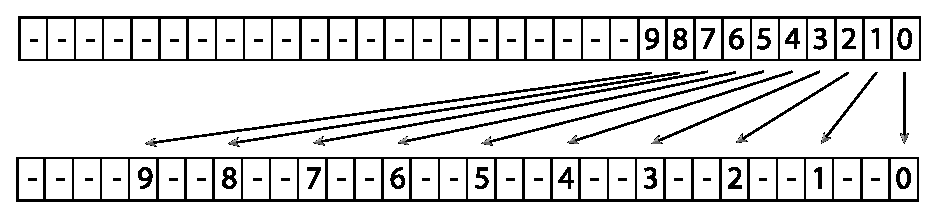
\includegraphics[width=0.75\linewidth]{chap04/LeftShift3.eps}
    \caption{移位以计算3D莫顿码。函数\refvar{LeftShift3}{()}接收32位整数值,
        且对于低10位,把第$i$位移到第$3i$位的位置——换句话说,向左移$2i$位。剩下全部位设为零。}
    \label{fig:4.9}
\end{figure}

实现该操作最明显的方法,即单独移动每一位,并不是最高效的
(它需要总共9次位移以及逻辑或来计算最终值)。
取而代之的是,我们可以把每位的移动分解为多个幂2尺寸的移位且一并把数位值移到其最终位置。
然后,所有需要移动给定幂2数位的位可以一并移动。
函数\refvar{LeftShift3}{()}实现了该计算,\reffig{4.10}展示了它如何工作的。
\begin{figure}[htbp]
    \centering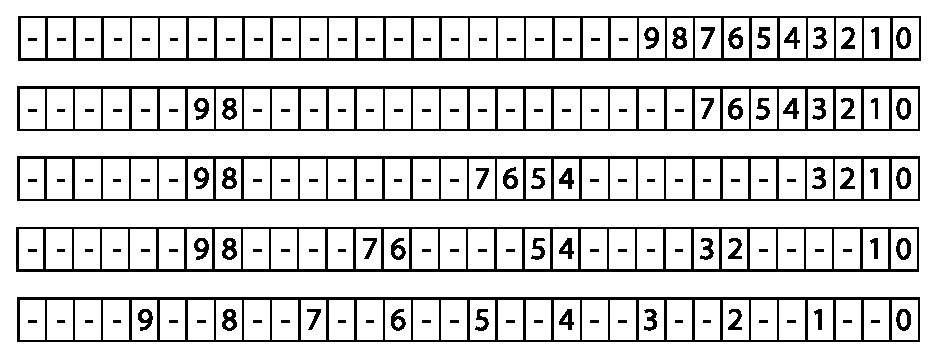
\includegraphics[width=0.75\linewidth]{Pictures/chap04/Mortonpow2decomposition.eps}
    \caption{莫顿移位的幂2分解。通过一系列幂2尺寸的移动来为每个3D坐标计算莫顿码执行移位。
        首先,位8和9向左移16位,这把位8放在了其最终位置。接着位4到7移动8位。
        移动4和2位后(适当掩模使每位最终都移动适当数位),所有数位都在正确的位置上。
        该计算由函数\refvar{LeftShift3}{()}实现。}
    \label{fig:4.10}
\end{figure}

\begin{lstlisting}
`\initcode{BVHAccel Utility Functions}{=}\initnext{BVHAccelUtilityFunctions}`
inline uint32_t `\initvar{LeftShift3}{}`(uint32_t x) {
    if (x == (1 << 10)) --x;
    x = (x | (x << 16)) & 0b00000011000000000000000011111111;
    x = (x | (x <<  8)) & 0b00000011000000001111000000001111;
    x = (x | (x <<  4)) & 0b00000011000011000011000011000011;
    x = (x | (x <<  2)) & 0b00001001001001001001001001001001;
    return x;
}
\end{lstlisting}

\refvar{EncodeMorton3}{()}接收每个分量都是$0$到$2^{10}$之间浮点值的3D坐标值。
它把这些值转换为整数然后通过展开三个10位量化值使第$i$位在位置$3i$上来计算莫顿码,
然后$y$位再移一位,$z$位再移两位,全部结果求或(\reffig{4.11})。
\begin{figure}[htbp]
    \centering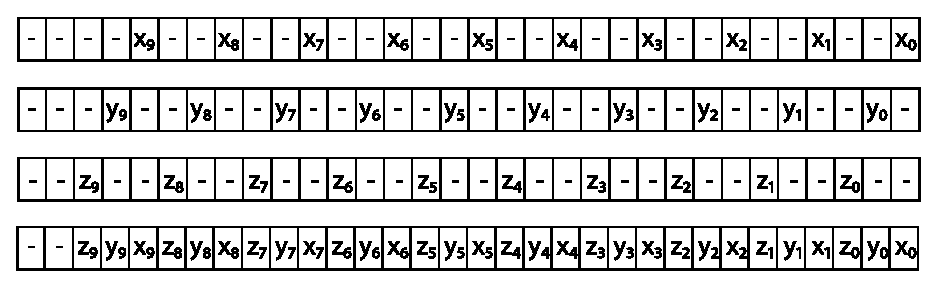
\includegraphics[width=0.75\linewidth]{chap04/Mortonxyzinterleave.eps}
    \caption{最终交错坐标值。有了\refvar{LeftShift3}{()}为$x$、$y$和$z$计算的交错值,
        最终莫顿编码值通过分别移动$y$和$z$一位和两位然后全部结果求或算得。}
    \label{fig:4.11}
\end{figure}

\begin{lstlisting}
`\refcode{BVHAccel Utility Functions}{+=}\lastnext{BVHAccelUtilityFunctions}`
inline uint32_t `\initvar{EncodeMorton3}{}`(const `\refvar{Vector3f}{}` &v) {
    return (`\refvar{LeftShift3}{}`(v.z) << 2) | (`\refvar{LeftShift3}{}`(v.y) << 1) |
            `\refvar{LeftShift3}{}`(v.x);
}
\end{lstlisting}

一旦计算了莫顿索引,我们将用\keyindex{基数排序}{radix sort}{}按莫顿索引值对
\newline{\ttfamily mortonPrims}排序。
我们已经发现对于BVH的构建,我们的基数排序实现明显快于使用我们系统标准库的{\ttfamily std::sort()}
(它是\keyindex{快速排序}{quicksort}{}和\keyindex{插入排序}{insertion sort}{}的混合)。
\begin{lstlisting}
`\initcode{Radix sort primitive Morton indices}{=}`
`\refvar{RadixSort}{}`(&mortonPrims);
\end{lstlisting}

回想基数排序和大多数排序算法的不同在于它不是基于比较一对值
而是基于依赖一些键值的桶子项。基数排序可用于排序整数值,
它从最右边数位到最左边每次排序一个数码。
它尤其值得每次对二进制值排序多个数码;
这样做减少了传递数据的次数。
这里的实现中,{\ttfamily bitsPerPass}设置每次传递处理的位数;
取值6后,我们有5次传递来排序30位。
\begin{lstlisting}
`\refcode{BVHAccel Utility Functions}{+=}\lastcode{BVHAccelUtilityFunctions}`
static void `\initvar{RadixSort}{}`(std::vector<`\refvar{MortonPrimitive}{}`> *v) {
    std::vector<`\refvar{MortonPrimitive}{}`> tempVector(v->size());
    constexpr int bitsPerPass = 6;
    constexpr int nBits = 30;
    constexpr int nPasses = nBits / bitsPerPass;
    for (int pass = 0; pass < nPasses; ++pass) {
        `\refcode{Perform one pass of radix sort, sorting bitsPerPass bits}{}`
    }
    `\refcode{Copy final result from tempVector, if needed}{}`
}
\end{lstlisting}

当前传递会排序{\ttfamily bitsPerPass}位,从{\ttfamily lowBit}开始。
\begin{lstlisting}
`\initcode{Perform one pass of radix sort, sorting bitsPerPass bits}{=}`
int lowBit = pass * bitsPerPass;
`\refcode{Set in and out vector pointers for radix sort pass}{}`
`\refcode{Count number of zero bits in array for current radix sort bit}{}`
`\refcode{Compute starting index in output array for each bucket}{}`
`\refcode{Store sorted values in output array}{}`
\end{lstlisting}

{\ttfamily in}和{\ttfamily out}引用分别对应于要排序的向量以及保存排序值的向量。
每次通过循环的传递都在输入向量{\ttfamily *v}和临时向量之间交替。
\begin{lstlisting}
`\initcode{Set in and out vector pointers for radix sort pass}{=}`
std::vector<`\refvar{MortonPrimitive}{}`> &in  = (pass & 1) ? tempVector : *v;
std::vector<`\refvar{MortonPrimitive}{}`> &out = (pass & 1) ? *v : tempVector;
\end{lstlisting}

如果我们每次传递中排序$n$位,则每个值可能落入的桶有$2^n$个。
我们先计数每个桶中会落入多少个值;这能让我们确定在输出数组中的何处保存排序值。
为了给当前值计算桶索引,该实现对索引移位使得在索引{\ttfamily lowBit}上的位
位于0号位,再掩模低处{\ttfamily bitsPerPass}个位。
\begin{lstlisting}
`\initcode{Count number of zero bits in array for current radix sort bit}{=}`
constexpr int nBuckets = 1 << bitsPerPass;
int bucketCount[nBuckets] = { 0 };
constexpr int bitMask = (1 << bitsPerPass) - 1;
for (const `\refvar{MortonPrimitive}{}` &mp : in) {
    int bucket = (mp.`\refvar{mortonCode}{}` >> lowBit) & bitMask;
    ++bucketCount[bucket];
}
\end{lstlisting}

有了每个桶中落入值的数量,我们就可以计算在输出数组中
每个桶的值开始处的偏移量;这就是之前的桶中落入值数量的和。
\begin{lstlisting}
`\initcode{Compute starting index in output array for each bucket}{=}`
int outIndex[nBuckets];
outIndex[0] = 0;
for (int i = 1; i < nBuckets; ++i)
    outIndex[i] = outIndex[i - 1] + bucketCount[i - 1];
\end{lstlisting}

现在我们知道每个桶在何处开始排序值了,
可以接收另一次图元传递来重算每个图元所在的桶并
将其\refvar{MortonPrimitive}{}保存在输出数组中。
这为当前这组数位完成了排序传递。
\begin{lstlisting}
`\initcode{Store sorted values in output array}{=}`
for (const `\refvar{MortonPrimitive}{}` &mp : in) {
    int bucket = (mp.`\refvar{mortonCode}{}` >> lowBit) & bitMask;
    out[outIndex[bucket]++] = mp;
}
\end{lstlisting}

当完成排序时,如果执行了奇数次基数排序传递,则最终排序值需要
从临时向量复制到原来传入\refvar{RadixSort}{()}的输出向量。
\begin{lstlisting}
`\initcode{Copy final result from tempVector, if needed}{}`
if (nPasses & 1)
    std::swap(*v, tempVector);
\end{lstlisting}

有了图元排序数组,我们将用附近的形心求得图元群集,
再在每个群集内创建图元上的LBVH。
这一步很适合并行化,因为通常有很多群集且每个群集都可以独立处理。
\begin{lstlisting}
`\initcode{Create LBVH treelets at bottom of BVH}{=}`
`\refcode{Find intervals of primitives for each treelet}{}`
`\refcode{Create LBVHs for treelets in parallel}{}`
\end{lstlisting}

每个图元群集都表示为一个\refvar{LBVHTreelet}{}。
它对群集中第一个图元在{\ttfamily mortonPrims}数组中的索引
以及后续图元的数量进行编码(见\reffig{4.12})。
\begin{lstlisting}
`\refcode{BVHAccel Local Declarations}{+=}\lastnext{BVHAccelLocalDeclarations}`
struct `\initvar{LBVHTreelet}{}` {
   int `\initvar{startIndex}{}`, `\initvar[LBVHTreelet:nPrimitives]{nPrimitives}{}`;
   `\refvar{BVHBuildNode}{}` *`\initvar{buildNodes}{}`;
};
\end{lstlisting}

\begin{figure}[htbp]
    \centering%LaTeX with PSTricks extensions
%%Creator: Inkscape 1.0.1 (3bc2e813f5, 2020-09-07)
%%Please note this file requires PSTricks extensions
\psset{xunit=.5pt,yunit=.5pt,runit=.5pt}
\begin{pspicture}(218.83000183,217.97000122)
{
\newrgbcolor{curcolor}{0 0 0}
\pscustom[linewidth=1,linecolor=curcolor]
{
\newpath
\moveto(0.5,217.47000122)
\lineto(217.47000122,217.47000122)
\lineto(217.47000122,0.5)
\lineto(0.5,0.5)
\closepath
}
}
{
\newrgbcolor{curcolor}{0 0 0}
\pscustom[linewidth=1,linecolor=curcolor]
{
\newpath
\moveto(54.66999817,217.83000122)
\lineto(54.66999817,0.74000549)
}
}
{
\newrgbcolor{curcolor}{0 0 0}
\pscustom[linewidth=1,linecolor=curcolor]
{
\newpath
\moveto(108.94000244,217.83000122)
\lineto(108.94000244,0.91000366)
}
}
{
\newrgbcolor{curcolor}{0 0 0}
\pscustom[linewidth=1,linecolor=curcolor]
{
\newpath
\moveto(163.19999695,217.83000122)
\lineto(163.19999695,0.30999756)
}
}
{
\newrgbcolor{curcolor}{0 0 0}
\pscustom[linewidth=1,linecolor=curcolor]
{
\newpath
\moveto(0.80000001,55.41000366)
\lineto(217.47999573,55.41000366)
}
}
{
\newrgbcolor{curcolor}{0 0 0}
\pscustom[linewidth=1,linecolor=curcolor]
{
\newpath
\moveto(0.68000001,109.66999817)
\lineto(217.25999451,109.66999817)
}
}
{
\newrgbcolor{curcolor}{0 0 0}
\pscustom[linewidth=1,linecolor=curcolor]
{
\newpath
\moveto(0.68000001,163.94000244)
\lineto(217.36999512,163.94000244)
}
}
{
\newrgbcolor{curcolor}{0 0 0}
\pscustom[linestyle=none,fillstyle=solid,fillcolor=curcolor]
{
\newpath
\moveto(128.87000036,82.82000732)
\curveto(128.87000036,86.10767491)(124.89535904,87.75354909)(122.57090879,85.42909884)
\curveto(120.24645854,83.10464859)(121.89233272,79.13000727)(125.18000031,79.13000727)
\curveto(128.46766789,79.13000727)(130.11354207,83.10464859)(127.78909182,85.42909884)
\curveto(125.46464157,87.75354909)(121.49000025,86.10767491)(121.49000025,82.82000732)
\curveto(121.49000025,79.53233974)(125.46464157,77.88646556)(127.78909182,80.21091581)
\curveto(130.11354207,82.53536606)(128.46766789,86.51000738)(125.18000031,86.51000738)
\curveto(121.89233272,86.51000738)(120.24645854,82.53536606)(122.57090879,80.21091581)
\curveto(124.89535904,77.88646556)(128.87000036,79.53233974)(128.87000036,82.82000732)
\closepath
}
}
{
\newrgbcolor{curcolor}{0 0 0}
\pscustom[linewidth=1,linecolor=curcolor,linestyle=dashed,dash=2]
{
\newpath
\moveto(106.09999847,96.31999969)
\lineto(143.87999725,96.31999969)
\lineto(143.87999725,69.21999931)
\lineto(106.09999847,69.21999931)
\closepath
}
}
{
\newrgbcolor{curcolor}{0 0 0}
\pscustom[linestyle=none,fillstyle=solid,fillcolor=curcolor]
{
\newpath
\moveto(76.74999762,150.77999878)
\curveto(76.74999762,154.06766637)(72.77535629,155.71354055)(70.45090604,153.3890903)
\curveto(68.12645579,151.06464005)(69.77232997,147.08999872)(73.05999756,147.08999872)
\curveto(76.34766514,147.08999872)(77.99353933,151.06464005)(75.66908908,153.3890903)
\curveto(73.34463883,155.71354055)(69.3699975,154.06766637)(69.3699975,150.77999878)
\curveto(69.3699975,147.49233119)(73.34463883,145.84645701)(75.66908908,148.17090726)
\curveto(77.99353933,150.49535751)(76.34766514,154.46999884)(73.05999756,154.46999884)
\curveto(69.77232997,154.46999884)(68.12645579,150.49535751)(70.45090604,148.17090726)
\curveto(72.77535629,145.84645701)(76.74999762,147.49233119)(76.74999762,150.77999878)
\closepath
}
}
{
\newrgbcolor{curcolor}{0 0 0}
\pscustom[linestyle=none,fillstyle=solid,fillcolor=curcolor]
{
\newpath
\moveto(179.88999701,139.84000397)
\curveto(179.88999701,143.12767155)(175.91535568,144.77354574)(173.59090543,142.44909549)
\curveto(171.26645518,140.12464524)(172.91232936,136.15000391)(176.19999695,136.15000391)
\curveto(179.48766453,136.15000391)(181.13353872,140.12464524)(178.80908847,142.44909549)
\curveto(176.48463822,144.77354574)(172.50999689,143.12767155)(172.50999689,139.84000397)
\curveto(172.50999689,136.55233638)(176.48463822,134.9064622)(178.80908847,137.23091245)
\curveto(181.13353872,139.5553627)(179.48766453,143.53000402)(176.19999695,143.53000402)
\curveto(172.91232936,143.53000402)(171.26645518,139.5553627)(173.59090543,137.23091245)
\curveto(175.91535568,134.9064622)(179.88999701,136.55233638)(179.88999701,139.84000397)
\closepath
}
}
{
\newrgbcolor{curcolor}{0 0 0}
\pscustom[linestyle=none,fillstyle=solid,fillcolor=curcolor]
{
\newpath
\moveto(44.64999914,38.22000122)
\curveto(44.64999914,41.50766881)(40.67535782,43.15354299)(38.35090757,40.82909274)
\curveto(36.02645732,38.50464249)(37.6723315,34.53000116)(40.95999908,34.53000116)
\curveto(44.24766667,34.53000116)(45.89354085,38.50464249)(43.5690906,40.82909274)
\curveto(41.24464035,43.15354299)(37.26999903,41.50766881)(37.26999903,38.22000122)
\curveto(37.26999903,34.93233363)(41.24464035,33.28645945)(43.5690906,35.6109097)
\curveto(45.89354085,37.93535995)(44.24766667,41.91000128)(40.95999908,41.91000128)
\curveto(37.6723315,41.91000128)(36.02645732,37.93535995)(38.35090757,35.6109097)
\curveto(40.67535782,33.28645945)(44.64999914,34.93233363)(44.64999914,38.22000122)
\closepath
}
}
{
\newrgbcolor{curcolor}{0 0 0}
\pscustom[linestyle=none,fillstyle=solid,fillcolor=curcolor]
{
\newpath
\moveto(143.66999578,199.77000046)
\curveto(143.66999578,203.05766804)(139.69535446,204.70354223)(137.37090421,202.37909198)
\curveto(135.04645396,200.05464173)(136.69232814,196.0800004)(139.97999573,196.0800004)
\curveto(143.26766331,196.0800004)(144.9135375,200.05464173)(142.58908725,202.37909198)
\curveto(140.264637,204.70354223)(136.28999567,203.05766804)(136.28999567,199.77000046)
\curveto(136.28999567,196.48233287)(140.264637,194.83645869)(142.58908725,197.16090894)
\curveto(144.9135375,199.48535919)(143.26766331,203.46000051)(139.97999573,203.46000051)
\curveto(136.69232814,203.46000051)(135.04645396,199.48535919)(137.37090421,197.16090894)
\curveto(139.69535446,194.83645869)(143.66999578,196.48233287)(143.66999578,199.77000046)
\closepath
}
}
{
\newrgbcolor{curcolor}{0 0 0}
\pscustom[linewidth=1,linecolor=curcolor]
{
\newpath
\moveto(143.66999578,199.77000046)
\curveto(143.66999578,203.05766804)(139.69535446,204.70354223)(137.37090421,202.37909198)
\curveto(135.04645396,200.05464173)(136.69232814,196.0800004)(139.97999573,196.0800004)
\curveto(143.26766331,196.0800004)(144.9135375,200.05464173)(142.58908725,202.37909198)
\curveto(140.264637,204.70354223)(136.28999567,203.05766804)(136.28999567,199.77000046)
\curveto(136.28999567,196.48233287)(140.264637,194.83645869)(142.58908725,197.16090894)
\curveto(144.9135375,199.48535919)(143.26766331,203.46000051)(139.97999573,203.46000051)
\curveto(136.69232814,203.46000051)(135.04645396,199.48535919)(137.37090421,197.16090894)
\curveto(139.69535446,194.83645869)(143.66999578,196.48233287)(143.66999578,199.77000046)
\closepath
}
}
{
\newrgbcolor{curcolor}{0 0 0}
\pscustom[linewidth=1,linecolor=curcolor,linestyle=dashed,dash=2]
{
\newpath
\moveto(123.81999969,214.10000134)
\lineto(155.86999893,214.10000134)
\lineto(155.86999893,185.96000195)
\lineto(123.81999969,185.96000195)
\closepath
}
}
{
\newrgbcolor{curcolor}{0 0 0}
\pscustom[linewidth=1,linecolor=curcolor,linestyle=dashed,dash=2]
{
\newpath
\moveto(33.40000153,171.63000107)
\lineto(113.13999939,171.63000107)
\lineto(113.13999939,130.4600029)
\lineto(33.40000153,130.4600029)
\closepath
}
}
{
\newrgbcolor{curcolor}{0 0 0}
\pscustom[linewidth=1,linecolor=curcolor,linestyle=dashed,dash=2]
{
\newpath
\moveto(167.86000061,162.25)
\lineto(184.28000069,162.25)
\lineto(184.28000069,117.95000076)
\lineto(167.86000061,117.95000076)
\closepath
}
}
{
\newrgbcolor{curcolor}{0 0 0}
\pscustom[linewidth=1,linecolor=curcolor,linestyle=dashed,dash=2]
{
\newpath
\moveto(18.29000092,64.80000305)
\lineto(63.37000275,64.80000305)
\lineto(63.37000275,11.6400032)
\lineto(18.29000092,11.6400032)
\closepath
}
}
\end{pspicture}

    \caption{LBVH小树的图元群集。图元形心聚类到覆盖其边界的均匀网格内。
        为每个格子中位于排序后的莫顿索引值连续段内的图元群集创建LBVH。}
    \label{fig:4.12}
\end{figure}

回想\reffig{4.8}中

\part{成像过程}
\chapterimage{Pictures/chap05/measure-one180-1260x630.png}
\chapter{颜色和辐射度学}\label{chap:颜色和辐射度学}
\setcounter{sidenote}{1}

为了精确描述光是怎样被表示和采样以计算图像的,
我们必须首先建立一些\keyindex{辐射度学}{radiometry}{}的背景——
\keyindex{电磁辐射}{electromagnetic radiation}{}在环境中的传播研究。
渲染中尤其感兴趣的是\keyindex{波长}{wavelength}{}($\lambda$)约在
380nm到780nm的电磁辐射\sidenote{译者注:{\normalfont nm}即长度单位纳米。$1$纳米=$10^{-9}$米。},
主要是人眼可见光\footnote{可感知波长的完整范围稍微超出了该区间,
但眼睛在这些波长上的敏感性低了许多量级。当绘制光谱曲线时常把范围360-830nm用作保守边界。}。
较短波长($\lambda\approx400\text{nm}$)是偏蓝色的,
中间波长($\lambda\approx550\text{nm}$)是绿色的,
而较长波长($\lambda\approx650\text{nm}$)是红色的。

本章中,我们将介绍描述电磁辐射的四个关键量:
\keyindex{通量}{flux}{}、\keyindex{强度}{intensity}{}、
\keyindex{辐射照度}{irradiance}{}和\keyindex{辐射亮度}{radiance}{}。
这些辐射量每一个都由它们的\keyindex{光谱功率分布}{spectral power distribution}{}(SPD)——
描述在各波长上的光量关于波长的函数。
pbrt中用定义于\refsec{光谱表示}的类\refvar{Spectrum}{}来表示SPD。

\section{光谱表示}\label{sec:光谱表示}

真实世界物体的SPD可能极其复杂;
\reffig{5.1}展示了荧光灯发光的频谱分布和柠檬皮反射率的频谱分布图。
用SPD做计算的渲染器需要紧实、高效且准确的方式表示像这样的函数。
实践中,可能需要在这些特性间作取舍。
\begin{figure}[htbp]
    \centering
    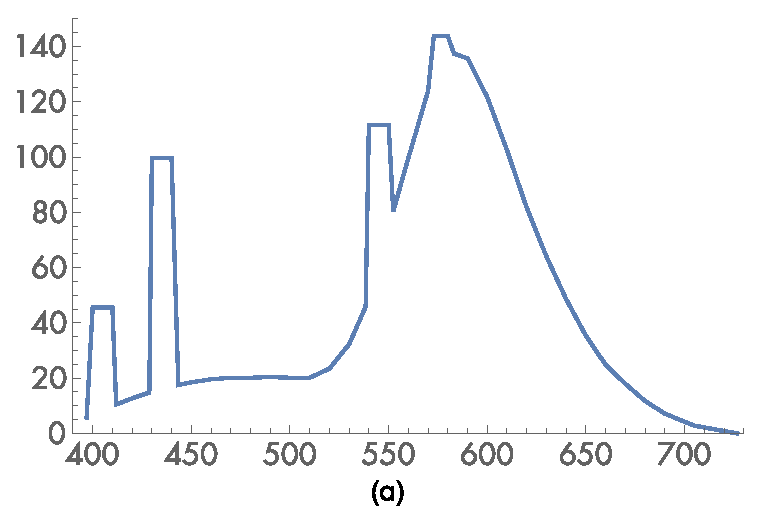
\includegraphics[width=0.45\linewidth]{chap05/fluorescent-spd.eps}\,\nolinebreak
    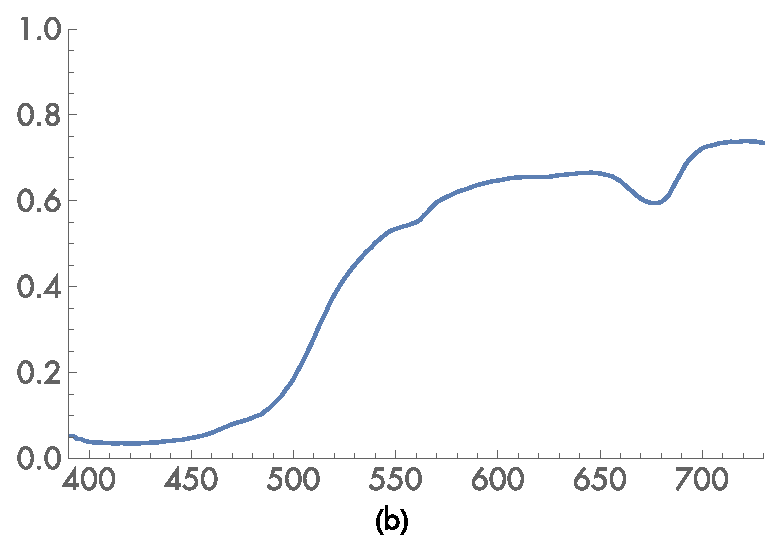
\includegraphics[width=0.45\linewidth]{chap05/lemonskin-spd.eps}
    \caption{(a)荧光灯的频谱分布和(b)柠檬皮的反射率。
    波长400nm左右是偏蓝光,而波长中段是绿色和黄色,波长700nm左右是红光。
    荧光灯的SPD甚至比这里展示的更加尖锐,SPD可归入到10nm范围内;
    它实际上是在单个离散频率上发出大量光。}
    \label{fig:5.1}
\end{figure}

研究这些问题的一般框架可以基于寻找
优良\keyindex{基函数}{basis function}{}以表示SPD的问题来开发。
基函数背后的思想是将可能的SPD函数的无限维空间映射到系数$c_i\in\mathbb{R}$的低维空间。
例如,一个平凡的基函数是常函数$B(\lambda)=1$。
任意SPD可以用等于其平均值的单个系数$c$以该基表示,
这样其近似就为$cB(\lambda)=c$。
很明显这是个很差的近似,因为大多数SPD都比这单个基函数所能准确表示的复杂得多。

在计算机图形学中已经为光谱表示研究了许多不同的基函数;
“扩展阅读”一节引用了关于该话题的许多文献和更多资源。
不同基函数集在关键运算上能提供截然不同的取舍,例如
将任意SPD转换为系数集(将其投影到基上)、
为由基表示的两个SPD之积给定的SPD计算系数等。
本章中,我们将介绍pbrt中可用于光谱的两种表示:\refvar{RGBSpectrum}{},
它遵循经典计算机图形学实践中用表示红、绿和蓝色混合的系数来表示SPD的做法,
以及\refvar{SampledSpectrum}{},它将SPD表示为在一个波长范围上采样点集。

\subsection{光谱类型}\label{sub:光谱类型}
整个pbrt中,我们都根据\refvar{Spectrum}{}类型
用一组特定内建运算符(加法、乘法等)仔细实现涉及SPD的全部计算。
\refvar{Spectrum}{}类型隐藏了所用特定光谱表示的细节,
这样改变系统的这些细节只需要改变\refvar{Spectrum}{}的实现;其他代码可保存不变。
\refvar{Spectrum}{}类型的实现在文件\href{https://github.com/mmp/pbrt-v3/blob/master/src/core/spectrum.h}{\ttfamily core/spectrum.h}和
\href{https://github.com/mmp/pbrt-v3/blob/master/src/core/spectrum.cpp}{\ttfamily core/spectrum.cpp}中。

pbrt中为\refvar{Spectrum}{}类型选择使用哪种光谱表示
在文件\href{https://github.com/mmp/pbrt-v3/blob/master/src/core/pbrt.h}{\ttfamily core/pbrt.h}中
由{\ttfamily typedef}完成。
pbrt默认使用更高效但不太精确的RGB表示。
\begin{lstlisting}
`\initcode{Global Forward Declarations}{=}\initnext{GlobalForwardDeclarations}`
typedef `\refvar{RGBSpectrum}{}` `\initvar{Spectrum}{}`;
// typedef \refvar{SampledSpectrum}{} Spectrum;
\end{lstlisting}

我们还没有把系统编写成在运行时解析选用哪个\refvar{Spectrum}{}表示;
为了切换到不同的表示,整个系统必须重新编译。
这一设计的一个优点是许多各种\refvar{Spectrum}{}方法可以实现为
能被编译器内联\sidenote{译者注:原文inlined。}的短函数,而不是弄成
需要通过相对较慢的虚拟方法调用机制唤起的独立运行函数。
内联像这样的常用短函数能给出性能上的巨大提升。
第二个优点是系统中持有\refvar{Spectrum}{}类型实例的结构可以直接保有它们
而不需要在运行时基于所选的光谱表示动态地分配它们。

\subsection{系数光谱实现}\label{sub:系数光谱实现}
本章实现的两种表示都基于排序固定数目的SPD样本。
因此,
\begin{lstlisting}
`\initcode{Spectrum Declarations}{=}\initnext{SpectrumDeclarations}`
template <int `\initvar{nSpectrumSamples}{}`> class `\initvar{CoefficientSpectrum}{}` {
public:
    `\refcode{CoefficientSpectrum Public Methods}{}`
    `\refcode{CoefficientSpectrum Public Data}{}`
protected:
    `\refcode{CoefficientSpectrum Protected Data}{}`
};
\end{lstlisting}

\begin{lstlisting}
`\initcode{CoefficientSpectrum Public Methods}{=}\initnext{CoefficientSpectrumPublicMethods}`
`\refvar{CoefficientSpectrum}{}`(`\refvar{Float}{}` v = 0.f) {
    for (int i = 0; i < `\refvar{nSpectrumSamples}{}`; ++i)
        `\refvar[CoefficientSpectrum::c]{c}{}`[i] = v;
}
\end{lstlisting}

\begin{lstlisting}
`\initcode{CoefficientSpectrum Protected Data}{=}`
`\refvar{Float}{}` `\initvar[CoefficientSpectrum::c]{c}{}`[`\refvar{nSpectrumSamples}{}`];
\end{lstlisting}

\begin{lstlisting}
`\refcode{CoefficientSpectrum Public Methods}{+=}\lastnext{CoefficientSpectrumPublicMethods}`
bool `\initvar{IsBlack}{}`() const {
    for (int i = 0; i < `\refvar{nSpectrumSamples}{}`; ++i)
        if (`\refvar[CoefficientSpectrum::c]{c}{}`[i] != 0.) return false;
    return true;
}
\end{lstlisting}

\section{类SampledSpectrum}\label{sec:类SampledSpectrum}
\refvar{SampledSpectrum}{}用\refvar{CoefficientSpectrum}{}基础结构
来表示在起始和结束波长之间均匀间隔采样的SPD。
波长覆盖范围从400nm到700nm——人类视觉系统最为敏感的可见光谱范围。
样本数量60一般足够为渲染准确表示复杂的SPD
(见“扩展阅读”一节了解SPD采样率要求的背景)。
因此,第一个样本表示波长范围$[400,405)$,第二个表示$[405,410)$,以此类推。
这些值很容易在此处按需修改。
\begin{lstlisting}
`\initcode{Spectrum Utility Declarations}{=}\initnext{SpectrumUtilityDeclarations}`
static const int `\initvar{sampledLambdaStart}{}` = 400;
static const int `\initvar{sampledLambdaEnd}{}` = 700;
static const int `\initvar{nSpectralSamples}{}` = 60;
\end{lstlisting}
\begin{lstlisting}
`\refcode{Spectrum Declarations}{+=}\lastnext{SpectrumDeclarations}`
class `\initvar{SampledSpectrum}{}` : public `\refvar{CoefficientSpectrum}{}`<`\refvar{nSpectralSamples}{}`> {
public:
    `\refcode{SampledSpectrum Public Methods}{}`
private:
    `\refcode{SampledSpectrum Private Data}{}`
};
\end{lstlisting}

通过从类\refvar{CoefficientSpectrum}{}继承,
\refvar{SampledSpectrum}{}自动拥有之前定义的所有基本光谱算术运算符。
留待为它定义的主要方法是从光谱数据初始化它以及将它表示的SPD转换为其他光谱表示(例如RGB)。
用常数SPD初始化它的构造函数很简单。
\begin{lstlisting}
`\initcode{SampledSpectrum Public Methods}{=}\initnext{SampledSpectrumPublicMethods}`
`\refvar{SampledSpectrum}{}`(`\refvar{Float}{}` v = 0.f) : `\refvar{CoefficientSpectrum}{}`(v) { }
\end{lstlisting}

光谱数据经常以一组样本$(\lambda_i,v_i)$提供给我们,
其中第$i$个样本有在波长$\lambda_i$处的某值$v_i$。
一般而言,样本可能有不规则间隔,可能比\refvar{SampledSpectrum}{}要存储的更多或更少
(见pbrt发行中路径{\ttfamily scenes/spds}下\sidenote{译者注:笔者没有找到该路径。}
pbrt所用的各种SPD,它们许多都有不规则间隔)。

方法\refvar[SampledSpectrum::FromSampled]{FromSampled}{()}取用在
给定波长{\ttfamily lambda}处的SPD样本值{\ttfamily v}数组
并用它们定义分段线性函数来表示SPD。
对于\refvar{SampledSpectrum}{}的每个SPD样本,
它用下面定义的功能函数\refvar{AverageSpectrumSamples}{()}
来计算分段线性函数在每个SPD样本对应的波长范围上的均值。
\begin{lstlisting}
`\refcode{SampledSpectrum Public Methods}{+=}\lastnext{SampledSpectrumPublicMethods}`
static `\refvar{SampledSpectrum}{}` `\initvar[SampledSpectrum::FromSampled]{FromSampled}{}`(const `\refvar{Float}{}` *lambda,
                                   const `\refvar{Float}{}` *v, int n) {
    `\refcode{Sort samples if unordered, use sorted for returned spectrum}{}`
    `\refvar{SampledSpectrum}{}` r;
    for (int i = 0; i < `\refvar{nSpectralSamples}{}`; ++i) {
        `\refcode{Compute average value of given SPD over th sample's range}{}`
    }
    return r;
}
\end{lstlisting}

函数\refvar{AverageSpectrumSamples}{()}要求值$(\lambda_i,v_i)$按波长排序。
{\initvar{SpectrumSamplesSorted}{()}}函数检查它们是不是;
如果不是,则{\initvar{SortSpectrumSamples}{()}}对它们排序。
注意我们为排序的样本分配新存储而不改变调用者传入的值;
一般而言,对于该函数(不需要担心其特定实现的这些要求)的用户
这样做可能并不是期望的行为。
我们这里不会介绍这两个函数的实现,因为它们很简单。
\begin{lstlisting}
`\initcode{Sort samples if unordered, use sorted for returned spectrum}{=}`
if (!`\refvar{SpectrumSamplesSorted}{}`(lambda, v, n)) {
    std::vector<`\refvar{Float}{}`> slambda(&lambda[0], &lambda[n]);
    std::vector<`\refvar{Float}{}`> sv(&v[0], &v[n]);
    `\refvar{SortSpectrumSamples}{}`(&slambda[0], &sv[0], n);
    return `\refvar[SampledSpectrum::FromSampled]{FromSampled}{}`(&slambda[0], &sv[0], n);
}
\end{lstlisting}

为计算第$i$个光谱样本的值,我们计算其对应的波长范围——
{\ttfamily lambda0}到{\ttfamily lambda1}——
并用函数\refvar{AverageSpectrumSamples}{()}计算该范围给定分段线性SPD的均值。
这是采样和重构的1D实例,第\refchap{采样与重构}会讨论该话题的更多细节。
\begin{lstlisting}
`\initcode{Compute average value of given SPD over th sample's range}{=}`
`\refvar{Float}{}` lambda0 = `\refvar{Lerp}{}`(`\refvar{Float}{}`(i) / `\refvar{Float}{}`(`\refvar{nSpectralSamples}{}`), 
                     `\refvar{sampledLambdaStart}{}`, `\refvar{sampledLambdaEnd}{}`);
`\refvar{Float}{}` lambda1 = `\refvar{Lerp}{}`(`\refvar{Float}{}`(i + 1) / `\refvar{Float}{}`(`\refvar{nSpectralSamples}{}`), 
                     `\refvar{sampledLambdaStart}{}`, `\refvar{sampledLambdaEnd}{}`);
r.`\refvar[CoefficientSpectrum::c]{c}{}`[i] = `\refvar{AverageSpectrumSamples}{}`(lambda, v, n, lambda0, lambda1);
\end{lstlisting}

\reffig{5.2}展示了\refvar{AverageSpectrumSamples}{()}采用的基础方法:
它在部分或完全位于波长范围内的样本间的每个线性段上迭代,
从{\ttfamily lambdaStart}到{\ttfamily lambdaEnd}。
对于每个这样的分段,它计算其范围上的均值,
用该段覆盖的波长范围缩放该均值,最后求这些值的和。
最终均值是该和除以整个波长范围。
\begin{figure}[htbp]
    \centering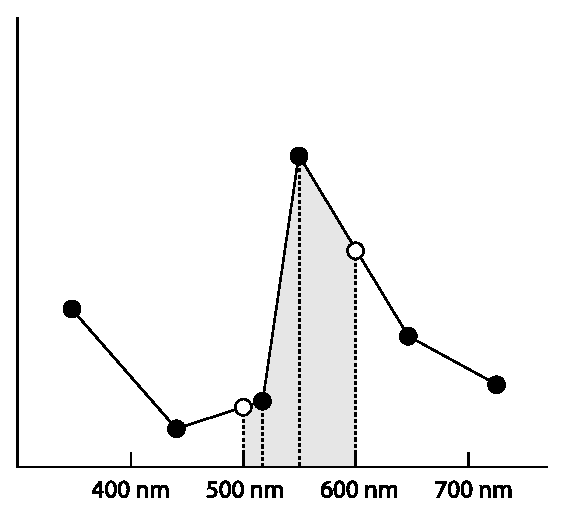
\includegraphics[width=0.4\linewidth]{chap05/IrregularSPDresample.eps}
    \caption{当重采样不规则定义的SPD时,我们需要计算由SPD样本定义的
        分段线性函数的均值。这里,我们想求从500nm到600nm的均值——图像下的阴影区。
        函数\refvar{AverageSpectrumSamples}{()}通过计算该图中虚线表示的每个区域的面积来完成。}
    \label{fig:5.2}
\end{figure}

\begin{lstlisting}
`\initcode{Spectrum Method Definitions}{=}\initnext{SpectrumMethodDefinitions}`
`\refvar{Float}{}` `\initvar{AverageSpectrumSamples}{}`(const `\refvar{Float}{}` *lambda, const `\refvar{Float}{}` *vals,
        int n, `\refvar{Float}{}` lambdaStart, `\refvar{Float}{}` lambdaEnd) {
    `\refcode{Handle cases with out-of-bounds range or single sample only}{}`
    `\refvar{Float}{}` sum = 0;
    `\refcode{Add contributions of constant segments before/after samples}{}`
    `\refcode{Advance to first relevant wavelength segment}{}`
    `\refcode{Loop over wavelength sample segments and add contributions}{}`
    return sum / (lambdaEnd - lambdaStart);
}
\end{lstlisting}

该函数从检查和处理极端情况开始,即求均值的波长范围
超出了提供的波长范围或只有单个样本进而均值计算是平凡的情况。
我们假设SPD在超出提供的采样范围外有常值(在两个端点的值);
如果这对于特定数据集不是一个合理的假设,则提供的数据应该在端点处有显式值(例如)0。
\begin{lstlisting}
`\initcode{Handle cases with out-of-bounds range or single sample only}{=}`
if (lambdaEnd   <= lambda[0])     return vals[0];
if (lambdaStart >= lambda[n - 1]) return vals[n - 1];
if (n == 1) return vals[0];
\end{lstlisting}

处理了这些情况后,下一步是检查看求均值的范围是否有部分超出第一个和/或最后一个样本值。
如果是,则我们累积常数段的贡献,用超出边界的波长范围缩放它。
\begin{lstlisting}
`\initcode{Add contributions of constant segments before/after samples}{=}`
if (lambdaStart < lambda[0])
    sum += vals[0] * (lambda[0] - lambdaStart);
if (lambdaEnd > lambda[n-1])
    sum += vals[n - 1] * (lambdaEnd - lambda[n - 1]);
\end{lstlisting}

现在我们推进到首个索引{\ttfamily i},
插值范围的起始波长重合于从$\lambda_i$到$\lambda_{i+1}$的一段。
这里更高效的实现是用二叉搜索而不是线性搜索
\footnote{甚至更高效的实现是利用一个事实即调用代码一般会需要
    在一段相邻波长范围上插值后的值,并可能在单次调用中接收了全部范围。
    然后可以为下一次插值从上一结尾处开始逐步寻找起始索引。}。
然而,该代码目前只在场景初始化时调用,所以目前不优化它不会影响渲染性能。
\begin{lstlisting}
`\initcode{Advance to first relevant wavelength segment}{=}`
int i = 0;
while (lambdaStart > lambda[i + 1]) ++i;
\end{lstlisting}

下面的循环在与求均值的范围重合的每个线性段上迭代。
对于每一段,它都通过求函数在这两点上取值的均值来
计算在波长范围{\ttfamily segLambdaStart}到{\ttfamily segLambdaEnd}上的均值。
该值依次用{\ttfamily interp()}计算,它是在给定波长的两个端点间线性插值的匿名函数。

下面调用{\ttfamily std::min()}和{\ttfamily std::max()}计算波长范围以在该段内做平均;
注意它们自然处理了{\ttfamily lambdaStart}、{\ttfamily lambdaEnd}或两者都在当前段内的情况。
\begin{lstlisting}
`\initcode{Loop over wavelength sample segments and add contributions}{=}`
auto interp = [lambda, vals](`\refvar{Float}{}` w, int i) {
    return `\refvar{Lerp}{}`((w - lambda[i]) / (lambda[i + 1] - lambda[i]),
                vals[i], vals[i + 1]);
};
for (; i+1 < n && lambdaEnd >= lambda[i]; ++i) {
    `\refvar{Float}{}` segLambdaStart = std::max(lambdaStart, lambda[i]);
    `\refvar{Float}{}` segLambdaEnd =   std::min(lambdaEnd,   lambda[i + 1]);
    sum += 0.5 * (interp(segLambdaStart, i) + interp(segLambdaEnd, i)) *
        (segLambdaEnd - segLambdaStart);
}
\end{lstlisting}

\subsection{XYZ颜色}\label{sub:XYZ颜色}
人类视觉系统的一个非凡性质是可只用三个浮点数为人类感知表示颜色。
颜色感知的\keyindex{三刺激理论}{tristimulus theory}{}说
用三个值$x_{\lambda},y_{\lambda}$和$z_{\lambda}$就能为人类观察者准确表示所有可见SPD。
给定发射SPD即$S(\lambda)$,通过积分它们与\keyindex{光谱匹配曲线}{spectral matching curve}{}
$X(\lambda),Y(\lambda)$和$Z(\lambda)$的积可算得这些值:
\begin{align}\label{eq:5.1}
    x_{\lambda} & =\int\limits_{\lambda}{S(\lambda)X(\lambda)\mathrm{d}\lambda}\, ,\nonumber \\
    y_{\lambda} & =\int\limits_{\lambda}{S(\lambda)Y(\lambda)\mathrm{d}\lambda}\, ,          \\
    z_{\lambda} & =\int\limits_{\lambda}{S(\lambda)Z(\lambda)\mathrm{d}\lambda}\, .\nonumber
\end{align}

这些曲线是由国际照明委员会\sidenote{译者注:法文Commission Internationale de l'Éclairage,
    英文International Commission on Illumination,是有关光学、照明、颜色和色度空间科学领域的国际组织,成立于1913年。}(CIE)
规范化机构在一系列以人类为测试对象的实验后决定的并画于\reffig{5.3}中。
一般认为这些匹配曲线通常类似于人类视网膜中三种色敏视锥细胞\sidenote{译者注:原文 color-sensitive cone。}的响应。
惊人的是,有截然不同分布的SPD可能有非常接近的$x_{\lambda},y_{\lambda}$和$z_{\lambda}$值。
对于人类观察者,这样的SPD实际上有一样的视觉呈现。
这样的光谱对称为\keyindex{同色异谱}{metamer}{}。
\begin{figure}[htbp]
    \centering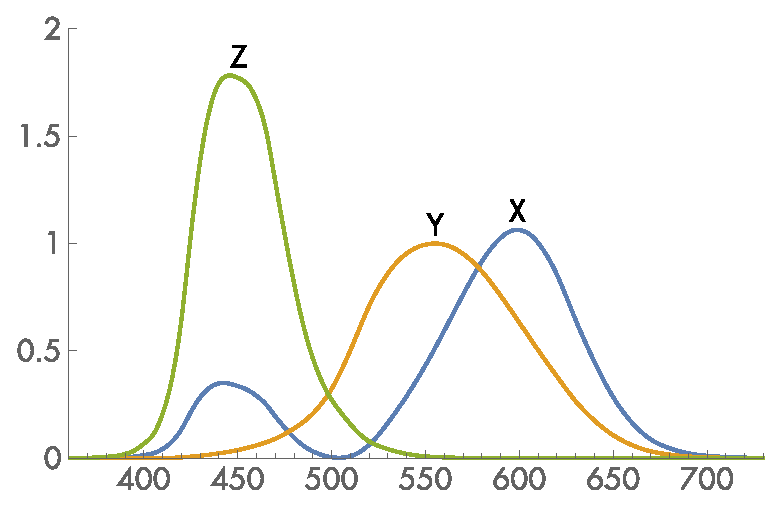
\includegraphics[width=0.5\linewidth]{chap05/matching-xyz.eps}
    \caption{对任意SPD计算XYZ值。用\refeq{5.1}让SPD与三个匹配曲线的每一个
    相乘并在其非零范围上积分以计算$x_{\lambda},y_{\lambda}$和$z_{\lambda}$值。}
    \label{fig:5.3}
\end{figure}

这给我们带来了关于光谱功率分布表示的一个微妙之处。
大部分颜色空间都希望模型颜色是对人类可见的,进而根据颜色感知的三刺激理论只需用三个系数。
尽管XYZ能很好地表示要对人类观察者显示的给定SPD,
但它对于光谱计算而言{\itshape 不是}特别好的基函数集。
例如,尽管XYZ值能很好地分别描述柠檬皮或荧光灯的感知颜色(回想\reffig{5.1}),
但它们各自的XYZ值之积给出的XYZ颜色可能明显不同于用其SPD更精确的表示相乘再计算出的XYZ值。

pbrt提供了标准$X(\lambda),Y(\lambda)$和$Z(\lambda)$相应曲线从360nm到830nm间隔1nm采样的值。
下面的数组中第$i$个样本的波长由\refvar{CIE\_lambda}{}的第$i$个元素给定;
用这种方式显式表示样本波长能更容易将XYZ样本传入到像\refvar{AverageSpectrumSamples}{()}
那样接收波长数组作为参数的函数。
\begin{lstlisting}
`\initcode{Spectral Data Declarations}{=}\initnext{SpectralDataDeclarations}`
static const int `\initvar{nCIESamples}{}` = 471;
extern const `\refvar{Float}{}` `\initvar{CIE\_X}{}`[`\refvar{nCIESamples}{}`];
extern const `\refvar{Float}{}` `\initvar{CIE\_Y}{}`[`\refvar{nCIESamples}{}`];
extern const `\refvar{Float}{}` `\initvar{CIE\_Z}{}`[`\refvar{nCIESamples}{}`];
extern const `\refvar{Float}{}` `\initvar{CIE\_lambda}{}`[`\refvar{nCIESamples}{}`];
\end{lstlisting}

\refvar{SampledSpectrum}{}用这些样本计算其光谱表示里的XYZ匹配曲线(即它们自己是\refvar{SampledSpectrum}{})。
\begin{lstlisting}
`\initcode{SampledSpectrum Private Data}{=}\initnext{SampledSpectrumPrivateData}`
static `\refvar{SampledSpectrum}{}` `\initvar[SampledSpectrum::X]{X}{}`, `\initvar[SampledSpectrum::Y]{Y}{}`, `\initvar[SampledSpectrum::Z]{Z}{}`;
\end{lstlisting}

\refvar{SampledSpectrum}{}的XYZ曲线在方法\refvar{SampledSpectrum::Init}{()}中算得,
它在系统启动时被定义于\refsec{初始化和渲染选项}\sidenote{译者注:原文标错了章节,已修正。}
的函数\refvar{pbrtInit}{()}调用。
\begin{lstlisting}
`\refcode{SampledSpectrum Public Methods}{+=}\lastnext{SampledSpectrumPublicMethods}`
static void `\initvar[SampledSpectrum::Init]{Init}{}`() {
    `\refcode{Compute XYZ matching functions for SampledSpectrum}{}`
    `\refcode{Compute RGB to spectrum functions for SampledSpectrum}{}`
}
\end{lstlisting}
\begin{lstlisting}
`\initcode{General pbrt Initialization}{=}`
`\refvar{SampledSpectrum}{}`::`\refvar[SampledSpectrum::Init]{Init}{}`();
\end{lstlisting}

为\refvar{SampledSpectrum}{}给定波长范围和样本数量,
为每个样本计算匹配函数的值只需计算样本的波长范围并利用\refvar{AverageSpectrumSamples}{()}例程。
\begin{lstlisting}
`\initcode{Compute XYZ matching functions for SampledSpectrum}{=}`
for (int i = 0; i < `\refvar{nSpectralSamples}{}`; ++i) {
    `\refvar{Float}{}` wl0 = `\refvar{Lerp}{}`(`\refvar{Float}{}`(i) / `\refvar{Float}{}`(`\refvar{nSpectralSamples}{}`), 
                     `\refvar{sampledLambdaStart}{}`, `\refvar{sampledLambdaEnd}{}`);
    `\refvar{Float}{}` wl1 = `\refvar{Lerp}{}`(`\refvar{Float}{}`(i + 1) / `\refvar{Float}{}`(`\refvar{nSpectralSamples}{}`), 
                     `\refvar{sampledLambdaStart}{}`, `\refvar{sampledLambdaEnd}{}`);
    `\refvar[SampledSpectrum::X]{X}{}`.`\refvar[CoefficientSpectrum::c]{c}{}`[i] = `\refvar{AverageSpectrumSamples}{}`(`\refvar{CIE\_lambda}{}`, `\refvar{CIE\_X}{}`, `\refvar{nCIESamples}{}`,
                                    wl0, wl1);
    `\refvar[SampledSpectrum::Y]{Y}{}`.`\refvar[CoefficientSpectrum::c]{c}{}`[i] = `\refvar{AverageSpectrumSamples}{}`(`\refvar{CIE\_lambda}{}`, `\refvar{CIE\_Y}{}`, `\refvar{nCIESamples}{}`,
                                    wl0, wl1);
    `\refvar[SampledSpectrum::Z]{Z}{}`.`\refvar[CoefficientSpectrum::c]{c}{}`[i] = `\refvar{AverageSpectrumSamples}{}`(`\refvar{CIE\_lambda}{}`, `\refvar{CIE\_Z}{}`, `\refvar{nCIESamples}{}`,
                                    wl0, wl1);
}
\end{lstlisting}

pbrt中所有\refvar{Spectrum}{}实现都必须提供将其SPD转换为$(x_{\lambda},y_{\lambda},z_{\lambda})$系数的方法。
例如,在更新图像像素的过程中就会调用该方法。
当\refvar{Spectrum}{}表示的沿相机射出的光线上的光提供给\refvar{Film}{}时,
\refvar{Film}{}最终将它们转换为用于存储和/或显示的RGB值时处理的第一步就是将SPD转换为XYZ系数。

为了计算XYZ系数,\refvar{SampledSpectrum}{}用黎曼和计算\refeq{5.1}的积分:
\begin{align*}
    x_{\lambda}\approx\frac{\lambda_{\text{end}}-\lambda_{\text{start}}}{N}\sum\limits_{i=0}^{N-1}{X_ic_i}\, ,
\end{align*}
并以此类推\sidenote{译者注:但是下面的代码中实际上还多除以了{\ttfamily CIE\_Y\_integral}。}。
\begin{lstlisting}
`\refcode{SampledSpectrum Public Methods}{+=}\lastnext{SampledSpectrumPublicMethods}`
void `\initvar{ToXYZ}{}`(`\refvar{Float}{}` xyz[3]) const {
    xyz[0] = xyz[1] = xyz[2] = 0.f;
    for (int i = 0; i < `\refvar{nSpectralSamples}{}`; ++i) {
        xyz[0] += `\refvar[SampledSpectrum::X]{X}{}`.`\refvar[CoefficientSpectrum::c]{c}{}`[i] * `\refvar[CoefficientSpectrum::c]{c}{}`[i];
        xyz[1] += `\refvar[SampledSpectrum::Y]{Y}{}`.`\refvar[CoefficientSpectrum::c]{c}{}`[i] * `\refvar[CoefficientSpectrum::c]{c}{}`[i];
        xyz[2] += `\refvar[SampledSpectrum::Z]{Z}{}`.`\refvar[CoefficientSpectrum::c]{c}{}`[i] * `\refvar[CoefficientSpectrum::c]{c}{}`[i];
    }
    `\refvar{Float}{}` scale = `\refvar{Float}{}`(`\refvar{sampledLambdaEnd}{}` - `\refvar{sampledLambdaStart}{}`) /
                  `\refvar{Float}{}`(CIE_Y_integral * `\refvar{nSpectralSamples}{}`);
    xyz[0] *= scale;
    xyz[1] *= scale;
    xyz[2] *= scale;
}
\end{lstlisting}

XYZ颜色的$y$系数与\keyindex{光亮度}{luminance}{}密切相关,
它度量颜色的感知亮度\sidenote{译者注:原文brightness。}。
亮度将在\refsub{光亮度与光度学}详细介绍。
我们提供了分开的方法单独计算$y$,因为经常只需要光谱的亮度
(例如第\refchap{光传输I:表面反射}、\refchap{光传输II:体积渲染}和\refchap{光传输III:双向方法}中的
一些光传输算法用亮度作为穿过场景的光路的相对重要性度量)。
\begin{lstlisting}
`\refcode{SampledSpectrum Public Methods}{+=}\lastnext{SampledSpectrumPublicMethods}`
`\refvar{Float}{}` `\initvar[SampledSpectrum::y]{y}{}`() const { 
    `\refvar{Float}{}` yy = 0.f;
    for (int i = 0; i < `\refvar{nSpectralSamples}{}`; ++i)
        yy += `\refvar[SampledSpectrum::Y]{Y}{}`.`\refvar[CoefficientSpectrum::c]{c}{}`[i] * `\refvar[CoefficientSpectrum::c]{c}{}`[i];
    return yy * `\refvar{Float}{}`(`\refvar{sampledLambdaEnd}{}` - `\refvar{sampledLambdaStart}{}`) /
        `\refvar{Float}{}`(`\refvar{nSpectralSamples}{}`);
}
\end{lstlisting}

\subsection{RGB颜色}\label{sub:RGB颜色}

当我们在显示器上显示RGB颜色时,实际展示的光谱基本上决定于三种光谱响应曲线的加权和,
红、绿、蓝各一种,由显示器的磷光体\sidenote{译者注:原文phosphor。}发出,例如LED
\sidenote{译者注:即light-emitting diode,发光二极管。}
或LCD\sidenote{译者注:即liquid-crystal display,液晶显示器。}元素,
或者等离子体胞\sidenote{译者注:原文plasma cell。}
\footnote{该模型确实作了简化,它忽略了显示器所作的任何额外处理;
    尤其是许多显示器对显示的值执行了非线性重映射。}。
\reffig{5.4}画出了LED显示器和LCD显示器发出的红、绿和蓝分布;
注意它们截然不同。
\begin{figure}[htbp]
    \centering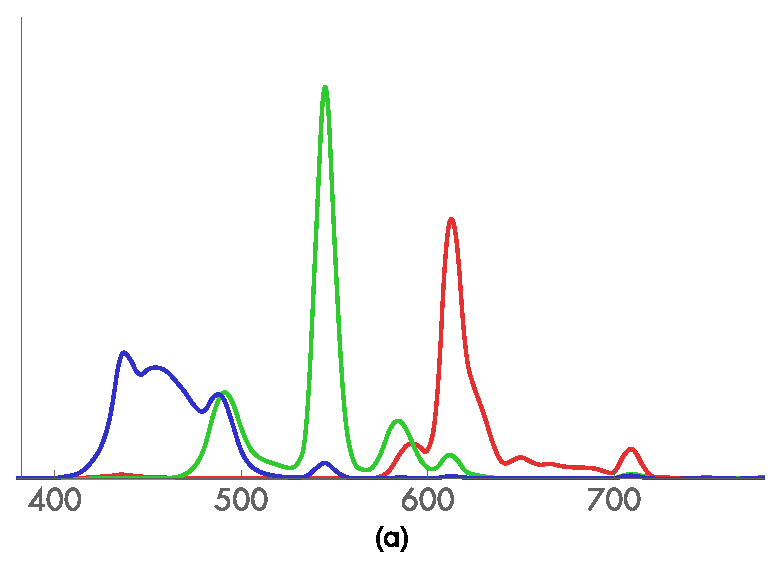
\includegraphics[width=0.45\linewidth]{chap05/lcd-display-spd.eps}\,
    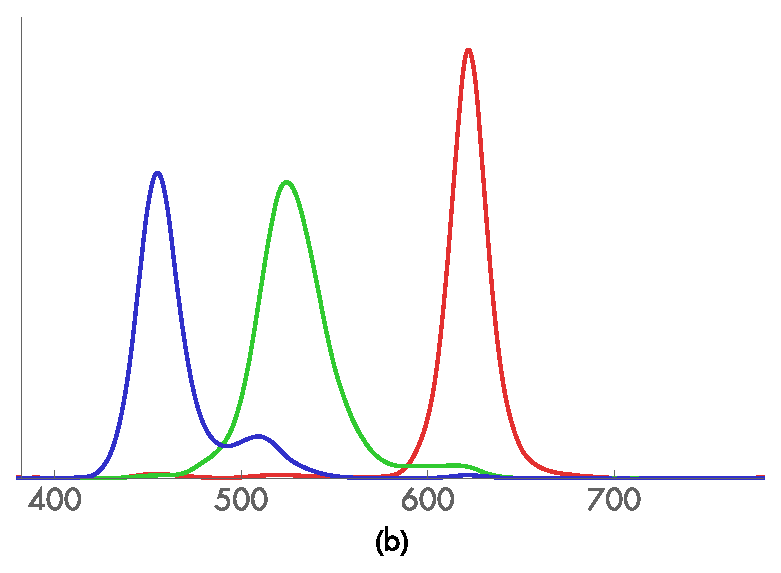
\includegraphics[width=0.45\linewidth]{chap05/led-display-spd.eps}
    \caption{LCD显示器和LED显示器的红、绿和蓝发射曲线。
    第一幅图展示了LCD显示器的曲线,第二幅图展示了LED的。
    这两种显示器有完全不同的发射配置({\itshape 感谢X-Rite公司提供数据})。}
    \label{fig:5.4}
\end{figure}

\reffig{5.5}依次展示了在这些显示器上显示RGB颜色$(0.6,0.3,0.2)$的SPD结果。
不出意料,结果中SPD也截然不同。这个例子说明了当用户选择RGB值时,
用他们提供的RGB值来描述特定颜色实际上只有在给定他们所用的显示器特性知识时才有意义。
\begin{figure}[htbp]
    \centering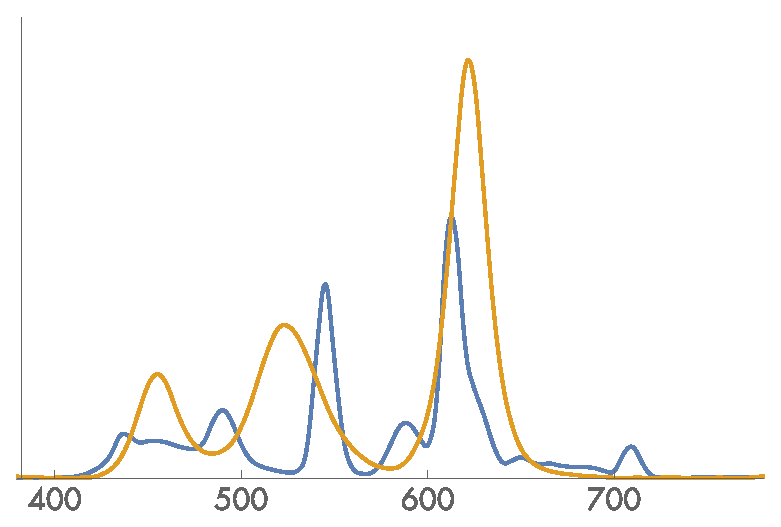
\includegraphics[width=0.5\linewidth]{chap05/same-rgb-different-display.eps}
    \caption{在LED和LCD显示器上显示RGB颜色$(0.6,0.3,0.2)$的SPD。
        甚至给定相同RGB值时得到的发射SPD也明显不同,因为\reffig{5.4}中的发射曲线不同。}
    \label{fig:5.5}
\end{figure}

给定SPD的表示$(x_{\lambda},y_{\lambda},z_{\lambda})$,
为感兴趣的显示器选定好定义红、绿和蓝的特定SPD集后,
我们可以将其转换为相应的RGB系数。
对于特定显示器,有了光谱响应曲线$R(\lambda),G(\lambda)$和$B(\lambda)$后,
可以通过积分响应曲线和SPD即$S(\lambda)$以及利用颜色感知的三刺激理论算得RGB系数:
\begin{align*}
    r & =\int R(\lambda)S(\lambda)\mathrm{d}\lambda=\int R(\lambda)(x_{\lambda}X(\lambda)+y_{\lambda}Y(\lambda)+z_{\lambda}Z(\lambda))\mathrm{d}\lambda                        \\
      & =x_{\lambda}\int R(\lambda)X(\lambda)\mathrm{d}\lambda+y_{\lambda}\int R(\lambda)Y(\lambda)\mathrm{d}\lambda+z_{\lambda}\int R(\lambda)Z(\lambda)\mathrm{d}\lambda\, .
\end{align*}

对于给定的响应曲线可以预先计算积$R(\lambda)X(\lambda)$的积分等,
使得能够把整个转换表达为矩阵:
\begin{align*}
    \left[\begin{array}{c}
            r \\ g\\ b
        \end{array}\right]=\left[
        \begin{array}{ccc}
            \int R(\lambda)X(\lambda)\mathrm{d}\lambda & \int R(\lambda)Y(\lambda)\mathrm{d}\lambda & \int R(\lambda)Z(\lambda)\mathrm{d}\lambda \\
            \int G(\lambda)X(\lambda)\mathrm{d}\lambda & \int G(\lambda)Y(\lambda)\mathrm{d}\lambda & \int G(\lambda)Z(\lambda)\mathrm{d}\lambda \\
            \int B(\lambda)X(\lambda)\mathrm{d}\lambda & \int B(\lambda)Y(\lambda)\mathrm{d}\lambda & \int B(\lambda)Z(\lambda)\mathrm{d}\lambda
        \end{array}
        \right]\left[\begin{array}{c}
            x_{\lambda} \\ y_{\lambda} \\ z_{\lambda}
        \end{array}\right]\, .
\end{align*}

pbrt中实现的转换例程是基于为高清电视定义的RGB光谱标准集的
\sidenote{译者注:这些系数的来由可见译者补充的\refsub{色度学}。}。
\begin{lstlisting}
`\refcode{Spectrum Utility Declarations}{+=}\lastnext{SpectrumUtilityDeclarations}`
inline void `\initvar{XYZToRGB}{}`(const `\refvar{Float}{}` xyz[3], `\refvar{Float}{}` rgb[3]) {
    rgb[0] =  3.240479f*xyz[0] - 1.537150f*xyz[1] - 0.498535f*xyz[2];
    rgb[1] = -0.969256f*xyz[0] + 1.875991f*xyz[1] + 0.041556f*xyz[2];
    rgb[2] =  0.055648f*xyz[0] - 0.204043f*xyz[1] + 1.057311f*xyz[2];
}
\end{lstlisting}

该矩阵的逆给出了把以特定RGB响应曲线表达的给定RGB值转换为$(x_{\lambda},y_{\lambda},z_{\lambda})$系数的系数。
\begin{lstlisting}
`\refcode{Spectrum Utility Declarations}{+=}\lastnext{SpectrumUtilityDeclarations}`
inline void `\initvar{RGBToXYZ}{}`(const `\refvar{Float}{}` rgb[3], `\refvar{Float}{}` xyz[3]) {
    xyz[0] = 0.412453f*rgb[0] + 0.357580f*rgb[1] + 0.180423f*rgb[2];
    xyz[1] = 0.212671f*rgb[0] + 0.715160f*rgb[1] + 0.072169f*rgb[2];
    xyz[2] = 0.019334f*rgb[0] + 0.119193f*rgb[1] + 0.950227f*rgb[2];
}
\end{lstlisting}

有了这些函数,\refvar{SampledSpectrum}{}可以通过首先转换到XYZ
再用实用函数\refvar{XYZToRGB}{()}转换为RGB系数。
\begin{lstlisting}
`\refcode{SampledSpectrum Public Methods}{+=}\lastnext{SampledSpectrumPublicMethods}`
void `\initvar[SampledSpectrum::ToRGB]{ToRGB}{}`(`\refvar{Float}{}` rgb[3]) const { 
    `\refvar{Float}{}` xyz[3];
    `\refvar{ToXYZ}{}`(xyz);
    `\refvar{XYZToRGB}{}`(xyz, rgb);
}
\end{lstlisting}

用方法\refvar[SampledSpectrum::ToRGBSpectrum]{ToRGBSpectrum}{()}也能很容易地创建\refvar{RGBSpectrum}{}。
\begin{lstlisting}
`\refcode{SampledSpectrum Public Methods}{+=}\lastnext{SampledSpectrumPublicMethods}`
`\refvar{RGBSpectrum}{}` `\initvar[SampledSpectrum::ToRGBSpectrum]{ToRGBSpectrum}{}`() const;
\end{lstlisting}

反过来从RGB或XYZ值转换为SPD并不简单:问题是高度欠约束的。
回想无数个不同的SPD有相同的$(x_{\lambda},y_{\lambda},z_{\lambda})$(进而以及RGB)系数。
因此,给定RGB或$(x_{\lambda},y_{\lambda},z_{\lambda})$值,可为其选择无数种可能的SPD。
有许多我们希望转换函数具有的准则:
\begin{itemize}
    \item 如果所有RGB系数有相同的值,则结果SPD应该为常数。
    \item 一般而言,希望算出的SPD是光滑的。大多数真实世界物体都有相对光滑的光谱。
          (尖锐光谱的主要源头是光源,特别是荧光灯。幸运的是,对于光源实际的光谱数据比反射率更常见。)
\end{itemize}

光滑目标是为什么把SPD构建为显示器的$R(\lambda),G(\lambda)$和$B(\lambda)$SPD的加权和不是好办法的原因:
如\reffig{5.4}所示,这些函数一般都是不规则且尖锐的,
因此它们的加权和不会是非常光滑的SPD。
该结果和给定RGB值是同色异谱的,它不太可能是实际物体SPD的准确表示。

这里我们实现了\citet{10.1080/10867651.1999.10487511}提出的将RGB转换为SPD
并尝试实现以上目标的的方法。
该方法基于一点观察即最好从为红、绿和蓝计算单独的光滑SPD开始,
这样用给定RGB系数计算它们的加权和然后转换回RGB给出的结果会接近于原来的RGB系数。
他通过数值优化过程发现了这样的光谱。

\citeauthor{10.1080/10867651.1999.10487511}观察到
可以对该方法做额外两点提升。
第一,比起用算得的恰好不是常数的红、绿和蓝SPD之和来表示常数光谱,
用常数SPD表示常数光谱更好。
第二,像黄色(红绿混合)那样由两种原色混合的颜色,
用它们预先计算的光滑SPD表示比用两种相应原色的SPD之和表示更好。

下面的数组保存了符合这些准则的SPD,
其样本的波长在\refvar{RGB2SpectLambda}{[]}
中(这些数据由Karl vom Berge生成)
\sidenote{译者注:cyan指蓝绿色,也称青色,magenta指紫红色,也称品红、洋红。}。
\begin{lstlisting}
`\refcode{Spectral Data Declarations}{+=}\lastnext{SpectralDataDeclarations}`
static const int `\initvar{nRGB2SpectSamples}{}` = 32;
extern const `\refvar{Float}{}` `\initvar{RGB2SpectLambda}{}`[`\refvar{nRGB2SpectSamples}{}`];
extern const `\refvar{Float}{}` `\initvar{RGBRefl2SpectWhite}{}`[`\refvar{nRGB2SpectSamples}{}`];
extern const `\refvar{Float}{}` `\initvar{RGBRefl2SpectCyan}{}`[`\refvar{nRGB2SpectSamples}{}`];
extern const `\refvar{Float}{}` `\initvar{RGBRefl2SpectMagenta}{}`[`\refvar{nRGB2SpectSamples}{}`];
extern const `\refvar{Float}{}` `\initvar{RGBRefl2SpectYellow}{}`[`\refvar{nRGB2SpectSamples}{}`];
extern const `\refvar{Float}{}` `\initvar{RGBRefl2SpectRed}{}`[`\refvar{nRGB2SpectSamples}{}`];
extern const `\refvar{Float}{}` `\initvar{RGBRefl2SpectGreen}{}`[`\refvar{nRGB2SpectSamples}{}`];
extern const `\refvar{Float}{}` `\initvar{RGBRefl2SpectBlue}{}`[`\refvar{nRGB2SpectSamples}{}`];
\end{lstlisting}

如果给定的RGB颜色为光源描述了光照,则用典型光源的光谱功率分布
计算用于反射率的转换表以定义“白色”会比用常数光谱得到更好结果。
数组\refvar{RGBIllum2Spect}{}使用了D65光谱功率分布,
它被CIE标准化为表示正午日光(\refsub{标准光源}将更多讨论D65光源)。
\begin{lstlisting}
`\refcode{Spectral Data Declarations}{+=}\lastcode{SpectralDataDeclarations}`
extern const `\refvar{Float}{}` `\initvar{RGBIllum2SpectWhite}{}`[`\refvar{nRGB2SpectSamples}{}`];
extern const `\refvar{Float}{}` `\initvar{RGBIllum2SpectCyan}{}`[`\refvar{nRGB2SpectSamples}{}`];
extern const `\refvar{Float}{}` `\initvar{RGBIllum2SpectMagenta}{}`[`\refvar{nRGB2SpectSamples}{}`];
extern const `\refvar{Float}{}` `\initvar{RGBIllum2SpectYellow}{}`[`\refvar{nRGB2SpectSamples}{}`];
extern const `\refvar{Float}{}` `\initvar{RGBIllum2SpectRed}{}`[`\refvar{nRGB2SpectSamples}{}`];
extern const `\refvar{Float}{}` `\initvar{RGBIllum2SpectGreen}{}`[`\refvar{nRGB2SpectSamples}{}`];
extern const `\refvar{Float}{}` `\initvar{RGBIllum2SpectBlue}{}`[`\refvar{nRGB2SpectSamples}{}`];
\end{lstlisting}

代码片\refcode{Compute RGB to spectrum functions for SampledSpectrum}{}由\linebreak
\refvar{SampledSpectrum::Init}{()}调用,此处不再介绍\sidenote{译者注:我补充回来了。};
它通过用函数\linebreak\refvar{AverageSpectrumSamples}{()}重采样
分布{\ttfamily RGBRefl2Spect}和{\ttfamily RGBIllum2Spect}来
初始化下列的\refvar{SampledSpectrum}{}值。
\begin{lstlisting}
`\refcode{SampledSpectrum Private Data}{+=}\lastnext{SampledSpectrumPrivateData}`
static `\refvar{SampledSpectrum}{}` `\initvar{rgbRefl2SpectWhite}{}`, `\initvar{rgbRefl2SpectCyan}{}`;
static `\refvar{SampledSpectrum}{}` `\initvar{rgbRefl2SpectMagenta}{}`, `\initvar{rgbRefl2SpectYellow}{}`;
static `\refvar{SampledSpectrum}{}` `\initvar{rgbRefl2SpectRed}{}`, `\initvar{rgbRefl2SpectGreen}{}`;
static `\refvar{SampledSpectrum}{}` `\initvar{rgbRefl2SpectBlue}{}`;
\end{lstlisting}
\begin{lstlisting}
`\refcode{SampledSpectrum Private Data}{+=}\lastcode{SampledSpectrumPrivateData}`
static `\refvar{SampledSpectrum}{}` `\initvar{rgbIllum2SpectWhite}{}`, `\initvar{rgbIllum2SpectCyan}{}`;
static `\refvar{SampledSpectrum}{}` `\initvar{rgbIllum2SpectMagenta}{}`, `\initvar{rgbIllum2SpectYellow}{}`;
static `\refvar{SampledSpectrum}{}` `\initvar{rgbIllum2SpectRed}{}`, `\initvar{rgbIllum2SpectGreen}{}`;
static `\refvar{SampledSpectrum}{}` `\initvar{rgbIllum2SpectBlue}{}`;
\end{lstlisting}
\begin{lstlisting}
`\initcode{Compute RGB to spectrum functions for SampledSpectrum}{=}`
for (int i = 0; i < `\refvar{nSpectralSamples}{}`; ++i) {
    `\refvar{Float}{}` wl0 = `\refvar{Lerp}{}`(`\refvar{Float}{}`(i) / `\refvar{Float}{}`(`\refvar{nSpectralSamples}{}`), 
                     `\refvar{sampledLambdaStart}{}`, `\refvar{sampledLambdaEnd}{}`);
    `\refvar{Float}{}` wl1 = `\refvar{Lerp}{}`(`\refvar{Float}{}`(i+1) / `\refvar{Float}{}`(`\refvar{nSpectralSamples}{}`), 
                     `\refvar{sampledLambdaStart}{}`, `\refvar{sampledLambdaEnd}{}`);
    `\refvar{rgbRefl2SpectWhite}{}`.`\refvar[CoefficientSpectrum::c]{c}{}`[i] = `\refvar{AverageSpectrumSamples}{}`(`\refvar{RGB2SpectLambda}{}`, `\refvar{rgbRefl2SpectWhite}{}`, 
        `\refvar{nRGB2SpectSamples}{}`, wl0, wl1);
    `\refvar{rgbRefl2SpectCyan}{}`.`\refvar[CoefficientSpectrum::c]{c}{}`[i] = `\refvar{AverageSpectrumSamples}{}`(`\refvar{RGB2SpectLambda}{}`, `\refvar{rgbRefl2SpectCyan}{}`, 
        `\refvar{nRGB2SpectSamples}{}`, wl0, wl1);
    `\refvar{rgbRefl2SpectMagenta}{}`.`\refvar[CoefficientSpectrum::c]{c}{}`[i] = `\refvar{AverageSpectrumSamples}{}`(`\refvar{RGB2SpectLambda}{}`, `\refvar{rgbRefl2SpectMagenta}{}`, 
        `\refvar{nRGB2SpectSamples}{}`, wl0, wl1);
    `\refvar{rgbRefl2SpectYellow}{}`.`\refvar[CoefficientSpectrum::c]{c}{}`[i] = `\refvar{AverageSpectrumSamples}{}`(`\refvar{RGB2SpectLambda}{}`, `\refvar{rgbRefl2SpectYellow}{}`, 
        `\refvar{nRGB2SpectSamples}{}`, wl0, wl1);
    `\refvar{rgbRefl2SpectRed}{}`.`\refvar[CoefficientSpectrum::c]{c}{}`[i] = `\refvar{AverageSpectrumSamples}{}`(`\refvar{RGB2SpectLambda}{}`, `\refvar{rgbRefl2SpectRed}{}`, 
        `\refvar{nRGB2SpectSamples}{}`, wl0, wl1);
    `\refvar{rgbRefl2SpectGreen}{}`.`\refvar[CoefficientSpectrum::c]{c}{}`[i] = `\refvar{AverageSpectrumSamples}{}`(`\refvar{RGB2SpectLambda}{}`, `\refvar{rgbRefl2SpectGreen}{}`, 
        `\refvar{nRGB2SpectSamples}{}`, wl0, wl1);
    `\refvar{rgbRefl2SpectBlue}{}`.`\refvar[CoefficientSpectrum::c]{c}{}`[i] = `\refvar{AverageSpectrumSamples}{}`(`\refvar{RGB2SpectLambda}{}`, `\refvar{rgbRefl2SpectBlue}{}`, 
        `\refvar{nRGB2SpectSamples}{}`, wl0, wl1);

    `\refvar{rgbIllum2SpectWhite}{}`.`\refvar[CoefficientSpectrum::c]{c}{}`[i] = `\refvar{AverageSpectrumSamples}{}`(`\refvar{RGB2SpectLambda}{}`, `\refvar{rgbIllum2SpectWhite}{}`, 
        `\refvar{nRGB2SpectSamples}{}`, wl0, wl1);
    `\refvar{rgbIllum2SpectCyan}{}`.`\refvar[CoefficientSpectrum::c]{c}{}`[i] = `\refvar{AverageSpectrumSamples}{}`(`\refvar{RGB2SpectLambda}{}`, `\refvar{rgbIllum2SpectCyan}{}`, 
        `\refvar{nRGB2SpectSamples}{}`, wl0, wl1);
    `\refvar{rgbIllum2SpectMagenta}{}`.`\refvar[CoefficientSpectrum::c]{c}{}`[i] = `\refvar{AverageSpectrumSamples}{}`(`\refvar{RGB2SpectLambda}{}`, `\refvar{rgbIllum2SpectMagenta}{}`, 
        `\refvar{nRGB2SpectSamples}{}`, wl0, wl1);
    `\refvar{rgbIllum2SpectYellow}{}`.`\refvar[CoefficientSpectrum::c]{c}{}`[i] = `\refvar{AverageSpectrumSamples}{}`(`\refvar{RGB2SpectLambda}{}`, `\refvar{rgbIllum2SpectYellow}{}`, 
        `\refvar{nRGB2SpectSamples}{}`, wl0, wl1);
    `\refvar{rgbIllum2SpectRed}{}`.`\refvar[CoefficientSpectrum::c]{c}{}`[i] = `\refvar{AverageSpectrumSamples}{}`(`\refvar{RGB2SpectLambda}{}`, `\refvar{rgbIllum2SpectRed}{}`, 
        `\refvar{nRGB2SpectSamples}{}`, wl0, wl1);
    `\refvar{rgbIllum2SpectGreen}{}`.`\refvar[CoefficientSpectrum::c]{c}{}`[i] = `\refvar{AverageSpectrumSamples}{}`(`\refvar{RGB2SpectLambda}{}`, `\refvar{rgbIllum2SpectGreen}{}`, 
        `\refvar{nRGB2SpectSamples}{}`, wl0, wl1);
    `\refvar{rgbIllum2SpectBlue}{}`.`\refvar[CoefficientSpectrum::c]{c}{}`[i] = `\refvar{AverageSpectrumSamples}{}`(`\refvar{RGB2SpectLambda}{}`, `\refvar{rgbIllum2SpectBlue}{}`, 
        `\refvar{nRGB2SpectSamples}{}`, wl0, wl1);
}
\end{lstlisting}

方法\refvar{SampledSpectrum::FromRGB}{()}将给定RGB值转换为完整的SPD。
除了RGB值,它还接收一个指明RGB值是表示曲面反射率还是光源的枚举值;
相应的{\ttfamily rgbIllum2Spect}或{\ttfamily rgbRefl2Spect}值用于该转换。
\begin{lstlisting}
`\refcode{Spectrum Utility Declarations}{+=}\lastcode{SpectrumUtilityDeclarations}`
enum class `\initvar{SpectrumType}{}` { `\initvar{Reflectance}{}`, `\initvar{Illuminant}{}` };
\end{lstlisting}
\begin{lstlisting}
`\refcode{Spectrum Method Definitions}{+=}\lastnext{SpectrumMethodDefinitions}`
`\refvar{SampledSpectrum}{}` `\initvar{SampledSpectrum::FromRGB}{}`(const `\refvar{Float}{}` rgb[3],
                                         `\refvar{SpectrumType}{}` type) {
    `\refvar{SampledSpectrum}{}` r;
    if (type == `\refvar{SpectrumType}{}`::`\refvar{Reflectance}{}`) {
        `\refcode{Convert reflectance spectrum to RGB}{}`
    } else {
        `\refcode{Convert illuminant spectrum to RGB}{}`
    }
    return r.`\refvar[CoefficientSpectrum::Clamp]{Clamp}{}`();
}
\end{lstlisting}

这里我们将展示反射率的转换过程。光源的计算也类似,只是用的不同的转换系数
\sidenote{译者注:这里我补充了光源的代码。}。
首先,实现确定红、绿、蓝哪个通道最小。
\begin{lstlisting}
`\initcode{Convert reflectance spectrum to RGB}{=}`
if (rgb[0] <= rgb[1] && rgb[0] <= rgb[2]) {
    `\refcode{Compute reflectance SampledSpectrum with rgb[0] as minimum}{}`
} else if (rgb[1] <= rgb[0] && rgb[1] <= rgb[2]) {
    `\refcode{Compute reflectance SampledSpectrum with rgb[1] as minimum}{}`
} else {
    `\refcode{Compute reflectance SampledSpectrum with rgb[2] as minimum}{}`
}
\end{lstlisting}
\begin{lstlisting}
`\initcode{Convert illuminant spectrum to RGB}{=}` 
if (rgb[0] <= rgb[1] && rgb[0] <= rgb[2]) {
    `\refcode{Compute illuminant SampledSpectrum with rgb[0] as minimum}{}`
} else if (rgb[1] <= rgb[0] && rgb[1] <= rgb[2]) {
    `\refcode{Compute illuminant SampledSpectrum with rgb[1] as minimum}{}`
} else {
    `\refcode{Compute illuminant SampledSpectrum with rgb[2] as minimum}{}`
}
\end{lstlisting}

这里是红色分量最小情况下的代码(绿色和蓝色类似这里书中就不介绍了)
\sidenote{译者注:我补充回来了。}。
如果红色最小,则我们知道绿色和蓝色有比红色更大的值。
这样我们可以通过给其赋予红色分量值乘以\refvar{rgbRefl2SpectWhite}{}中的
白色光谱来开始转换最终要返回的SPD。
完成后,RGB值中剩下要处理的是$(0,g-r,b-r)$。
代码依次确定剩下两个分量谁最小。
该值乘以青色\sidenote{译者注:原文cyan。}(绿蓝)光谱并加到结果中,
我们还剩下$(0,g-b,0)$或$(0,0,b-g)$。
基于绿色或蓝色通道哪一个非零,绿色或蓝色通道SPD被剩余部分缩放完成转换。
\begin{lstlisting}
`\initcode{Compute reflectance SampledSpectrum with rgb[0] as minimum}{=}`
r += rgb[0] * `\refvar{rgbRefl2SpectWhite}{}`;
if (rgb[1] <= rgb[2]) {
    r += (rgb[1] - rgb[0]) * `\refvar{rgbRefl2SpectCyan}{}`;
    r += (rgb[2] - rgb[1]) * `\refvar{rgbRefl2SpectBlue}{}`;
} else {
    r += (rgb[2] - rgb[0]) * `\refvar{rgbRefl2SpectCyan}{}`;
    r += (rgb[1] - rgb[2]) * `\refvar{rgbRefl2SpectGreen}{}`;
}
\end{lstlisting}
\begin{lstlisting}
`\initcode{Compute reflectance SampledSpectrum with rgb[1] as minimum}{=}`
r += rgb[1] * `\refvar{rgbRefl2SpectWhite}{}`;
if (rgb[0] <= rgb[2]) {
    r += (rgb[0] - rgb[1]) * `\refvar{rgbRefl2SpectMagenta}{}`;
    r += (rgb[2] - rgb[0]) * `\refvar{rgbRefl2SpectBlue}{}`;
} else {
    r += (rgb[2] - rgb[1]) * `\refvar{rgbRefl2SpectMagenta}{}`;
    r += (rgb[0] - rgb[2]) * `\refvar{rgbRefl2SpectRed}{}`;
}
\end{lstlisting}
\begin{lstlisting}
`\initcode{Compute reflectance SampledSpectrum with rgb[2] as minimum}{=}`
r += rgb[2] * `\refvar{rgbRefl2SpectWhite}{}`;
if (rgb[0] <= rgb[1]) {
    r += (rgb[0] - rgb[2]) * `\refvar{rgbRefl2SpectYellow}{}`;
    r += (rgb[1] - rgb[0]) * `\refvar{rgbRefl2SpectGreen}{}`;
} else {
    r += (rgb[1] - rgb[2]) * `\refvar{rgbRefl2SpectYellow}{}`;
    r += (rgb[0] - rgb[1]) * `\refvar{rgbRefl2SpectRed}{}`;
}
\end{lstlisting}
\begin{lstlisting}
`\initcode{Compute illuminant SampledSpectrum with rgb[0] as minimum}{=}`
r += rgb[0] * `\refvar{rgbIllum2SpectWhite}{}`;
if (rgb[1] <= rgb[2]) {
    r += (rgb[1] - rgb[0]) * `\refvar{rgbIllum2SpectCyan}{}`;
    r += (rgb[2] - rgb[1]) * `\refvar{rgbIllum2SpectBlue}{}`;
} else {
    r += (rgb[2] - rgb[0]) * `\refvar{rgbIllum2SpectCyan}{}`;
    r += (rgb[1] - rgb[2]) * `\refvar{rgbIllum2SpectGreen}{}`;
}
\end{lstlisting}
\begin{lstlisting}
`\initcode{Compute illuminant SampledSpectrum with rgb[1] as minimum}{=}`
r += rgb[1] * `\refvar{rgbIllum2SpectWhite}{}`;
if (rgb[0] <= rgb[2]) {
    r += (rgb[0] - rgb[1]) * `\refvar{rgbIllum2SpectMagenta}{}`;
    r += (rgb[2] - rgb[0]) * `\refvar{rgbIllum2SpectBlue}{}`;
} else {
    r += (rgb[2] - rgb[1]) * `\refvar{rgbIllum2SpectMagenta}{}`;
    r += (rgb[0] - rgb[2]) * `\refvar{rgbIllum2SpectRed}{}`;
}
\end{lstlisting}
\begin{lstlisting}
`\initcode{Compute illuminant SampledSpectrum with rgb[2] as minimum}{=}`
r += rgb[2] * `\refvar{rgbIllum2SpectWhite}{}`;
if (rgb[0] <= rgb[1]) {
    r += (rgb[0] - rgb[2]) * `\refvar{rgbIllum2SpectYellow}{}`;
    r += (rgb[1] - rgb[0]) * `\refvar{rgbIllum2SpectGreen}{}`;
} else {
    r += (rgb[1] - rgb[2]) * `\refvar{rgbIllum2SpectYellow}{}`;
    r += (rgb[0] - rgb[1]) * `\refvar{rgbIllum2SpectRed}{}`;
}
\end{lstlisting}

有了从RGB转换的方法,从XYZ颜色转换也很容易。
我们首先从XYZ转换到RGB然后再用方法\refvar[SampledSpectrum::FromRGB]{FromRGB}{()}。
\begin{lstlisting}
`\refcode{SampledSpectrum Public Methods}{+=}\lastcode{SampledSpectrumPublicMethods}`
static `\refvar{SampledSpectrum}{}` `\initvar[SampledSpectrum::FromXYZ]{FromXYZ}{}`(const `\refvar{Float}{}` xyz[3],
        `\refvar{SpectrumType}{}` type = `\refvar{SpectrumType}{}`::`\refvar{Reflectance}{}`) {
    `\refvar{Float}{}` rgb[3];
    `\refvar{XYZToRGB}{}`(xyz, rgb);
    return `\refvar[SampledSpectrum::FromRGB]{FromRGB}{}`(rgb, type);
}
\end{lstlisting}

最后,我们再次用上述基础提供了转换类\refvar{RGBSpectrum}{}的实例的构造函数。
\begin{lstlisting}
`\refcode{Spectrum Method Definitions}{+=}\lastnext{SpectrumMethodDefinitions}`
`\refvar{SampledSpectrum}{}`::`\refvar{SampledSpectrum}{}`(const `\refvar{RGBSpectrum}{}` &r, `\refvar{SpectrumType}{}` t) {
    `\refvar{Float}{}` rgb[3];
    r.`\refvar[SampledSpectrum::ToRGB]{ToRGB}{}`(rgb);
    *this = `\refvar{SampledSpectrum}{}`::`\refvar[SampledSpectrum::FromRGB]{FromRGB}{}`(rgb, t);
}
\end{lstlisting}

\section{RGBSpectrum的实现}\label{sec:RGBSpectrum的实现}

这里\refvar{RGBSpectrum}{}的实现用红绿蓝分量的加权和表示SPD。
回想该表示是定义病态的:给定两个不同的计算机显示器,
让它们显示相同RGB值并不会让它们发射相同的SPD。
因此,为了给一组RGB值指定实际的SPD,我们必须知道定义时所依据的显示器原色;
这些信息一般不会随RGB值提供。

然而RGB表示很方便:几乎所有3D建模和设计工具都使用RGB颜色,
大多数3D内容都用RGB指定。
此外,它的计算和存储很高效,只需要三个浮点值表示。
我们的\refvar{RGBSpectrum}{}实现继承自\refvar{CoefficientSpectrum}{},
指定三个分量存储。
因此,之前定义的所有算术运算符都自动地适用于\refvar{RGBSpectrum}{}。
\begin{lstlisting}
`\refcode{Spectrum Declarations}{+=}\lastcode{SpectrumDeclarations}`
class `\initvar{RGBSpectrum}{}` : public `\refvar{CoefficientSpectrum}{}`<3> {
public:
    `\refcode{RGBSpectrum Public Methods}{}`
};
\end{lstlisting}
\begin{lstlisting}
`\initcode{RGBSpectrum Public Methods}{=}\initnext{RGBSpectrumPublicMethods}`
`\refvar{RGBSpectrum}{}`(`\refvar{Float}{}` v = 0.f) : `\refvar{CoefficientSpectrum}{}`<3>(v) { }
`\refvar{RGBSpectrum}{}`(const `\refvar{CoefficientSpectrum}{}`<3> &v) 
    : `\refvar{CoefficientSpectrum}{}`<3>(v) { }
\end{lstlisting}

除了基本算术运算,\refvar{RGBSpectrum}{}还需要提供方法来与XYZ和RGB表示互相转换。
这些对于\refvar{RGBSpectrum}{}是容易的。
注意\refvar[RGBSpectrum::FromRGB]{FromRGB}{()}接收像该方法的
\refvar{SampledSpectrum}{}实例那样的\refvar{SpectrumType}{}参数。
尽管这里没有使用,但这两个类的{\ttfamily FromRGB()}方法
必须有匹配的特征,这样系统剩下的部分可以一致地调用它们而不用管用的是哪种光谱表示。
\begin{lstlisting}
`\refcode{RGBSpectrum Public Methods}{+=}\lastnext{RGBSpectrumPublicMethods}`
static `\refvar{RGBSpectrum}{}` `\initvar[RGBSpectrum::FromRGB]{FromRGB}{}`(const `\refvar{Float}{}` rgb[3],
        `\refvar{SpectrumType}{}` type = `\refvar{SpectrumType}{}`::`\refvar{Reflectance}{}`) {
    `\refvar{RGBSpectrum}{}` s;
    s.`\refvar[CoefficientSpectrum::c]{c}{}`[0] = rgb[0];
    s.`\refvar[CoefficientSpectrum::c]{c}{}`[1] = rgb[1];
    s.`\refvar[CoefficientSpectrum::c]{c}{}`[2] = rgb[2];
    return s;
}
\end{lstlisting}

同样,光谱表示必须能将其自己转换为RGB值。
对于\refvar{RGBSpectrum}{},该实现可以回避用什么特定RGB原色
来表示光谱分布的问题而只用假设原色与表示该色所正在用的相同并直接返回RGB系数。
\begin{lstlisting}
`\refcode{RGBSpectrum Public Methods}{+=}\lastnext{RGBSpectrumPublicMethods}`
void `\initvar[RGBSpectrum::ToRGB]{ToRGB}{}`(`\refvar{Float}{}` *rgb) const {
    rgb[0] = `\refvar[CoefficientSpectrum::c]{c}{}`[0];
    rgb[1] = `\refvar[CoefficientSpectrum::c]{c}{}`[1];
    rgb[2] = `\refvar[CoefficientSpectrum::c]{c}{}`[2];
}
\end{lstlisting}

所有光谱表示必须也能将其转换为\refvar{RGBSpectrum}{}对象。这在此处也很简单。
\begin{lstlisting}
`\refcode{RGBSpectrum Public Methods}{+=}\lastnext{RGBSpectrumPublicMethods}`
const `\refvar{RGBSpectrum}{}` &`\initvar[RGBSpectrum::ToRGBSpectrum]{ToRGBSpectrum}{}`() const {
    return *this;
}
\end{lstlisting}

{\initvar{RGBSpectrum::ToXYZ}{()}}、{\initvar{RGBSpectrum::FromXYZ}{()}}
和{\initvar{RGBSpectrum::y}{()}}的实现都基于上面定义的函数\refvar{RGBToXYZ}{()}
和\refvar{XYZToRGB}{()},此处不再介绍。

为了从任意采样的SPD创建RGB光谱,\refvar[RGBSpectrum::FromSampled]{FromSampled}{()}将
光谱转换为XYZ然后转为RGB。
它用实用函数\refvar{InterpolateSpectrumSamples}{()}按1nm步长
在存在CIE匹配函数对应值的每个波长处代入该分段线性采样的光谱。
然后它用该值计算黎曼和以逼近XYZ积分。
\begin{lstlisting}
`\refcode{RGBSpectrum Public Methods}{+=}\lastcode{RGBSpectrumPublicMethods}`
static `\refvar{RGBSpectrum}{}` `\initvar[RGBSpectrum::FromSampled]{FromSampled}`(const `\refvar{Float}{}` *lambda, const `\refvar{Float}{}` *v,
                               int n) {
    `\refcode{Sort samples if unordered, use sorted for returned spectrum}{=}`
    `\refvar{Float}{}` xyz[3] = { 0, 0, 0 };
    for (int i = 0; i < `\refvar{nCIESamples}{}`; ++i) {
        `\refvar{Float}{}` val = `\refvar{InterpolateSpectrumSamples}{}`(lambda, v, n,
                                               `\refvar{CIE\_lambda}{}`[i]);
        xyz[0] += val * `\refvar{CIE\_X}{}`[i];
        xyz[1] += val * `\refvar{CIE\_Y}{}`[i];
        xyz[2] += val * `\refvar{CIE\_Z}{}`[i];
    }
    `\refvar{Float}{}` scale = `\refvar{Float}{}`(`\refvar{CIE\_lambda}{}`[`\refvar{nCIESamples}{}`-1] - `\refvar{CIE\_lambda}{}`[0]) /
        `\refvar{Float}{}`(CIE_Y_integral * `\refvar{nCIESamples}{}`);
    xyz[0] *= scale;
    xyz[1] *= scale;
    xyz[2] *= scale;
    return `\refvar[RGBSpectrum::FromXYZ]{FromXYZ}{}`(xyz);    
}
\end{lstlisting}

\refvar{InterpolateSpectrumSamples}{()}接收可能是不规则采样的波长
和SPD值集$(\lambda_i,v_i)$并在框住$\lambda$的两个样本值之间线性插值以
返回在给定波长$\lambda$处的SPD值。
定义于\refchap{实用工具}的函数\refvar{FindInterval}{()}在
排了序的波长数组{\ttfamily lambda}中执行二分搜索寻找包含{\ttfamily l}的区间。
\begin{lstlisting}
`\refcode{Spectrum Method Definitions}{+=}\lastnext{SpectrumMethodDefinitions}`
`\refvar{Float}{}` `\initvar{InterpolateSpectrumSamples}{}`(const `\refvar{Float}{}` *lambda, const `\refvar{Float}{}` *vals,
                                 int n, `\refvar{Float}{}` l) {
    if (l <= lambda[0])     return vals[0];
    if (l >= lambda[n - 1]) return vals[n - 1];
    int offset = `\refvar{FindInterval}{}`(n,
        [&](int index) { return lambda[index] <= l; });
    `\refvar{Float}{}` t = (l - lambda[offset]) / (lambda[offset+1] - lambda[offset]);
    return `\refvar{Lerp}{}`(t, vals[offset], vals[offset + 1]);
}
\end{lstlisting}

\section{辐射度学}\label{sec:辐射度学}
 
\keyindex{辐射度学}{radiometry}{}提供了一系列描述光传播与反射的思想和数学工具。
它为贯穿本书剩余部分的渲染算法构建了推导的基础。
有趣的是,辐射度学不是用物理光学基本原理推导产生的,
而是基于穿过空间的粒子流来对光进行抽象并建立的。
因此,尽管辐射度学和\keyindex{麦克斯韦方程组}{Maxwell's equations}{}之间
已经建立了联系,为辐射度学提供了坚实的物理基础,
但像光的\keyindex{偏振}{polarization}{}
\sidenote{译者注:指横波能够朝着不同方向振荡的性质。}
那样的效应并不符合该框架。

\keyindex{辐射转移}{radiative transfer}{}是关于辐射能量转移现象的研究。
它基于辐射度量原则并在\keyindex{几何光学}{geometrical optics}{}
\sidenote{译者注:原文写作geometric optics。}层面上操作,
其中光的宏观性质足以描述光如何与比其波长大得多的物体相交。
与光的\keyindex{波动光学}{wave optics}{}模型中的现象结合并不罕见,
但这些结果需要用辐射转移的基本抽象语言来表达。
(\citet{PREISENDORFER19653}已经将辐射转移理论与
麦克斯韦描述电磁场的经典方程组联系起来。
他的框架既论证了它们的等价性又使得把一个世界观的结果应用到另一个世界观更容易了。
\citet{Fante:81}在该领域做了更多最近的工作。)

用这种方法就能描述光和与其波长大小接近的物体相交,
进而对\keyindex{色散}{dispersion}{}\sidenote{译者注:经典的棱镜色散实验。}
\begin{marginfigure}
    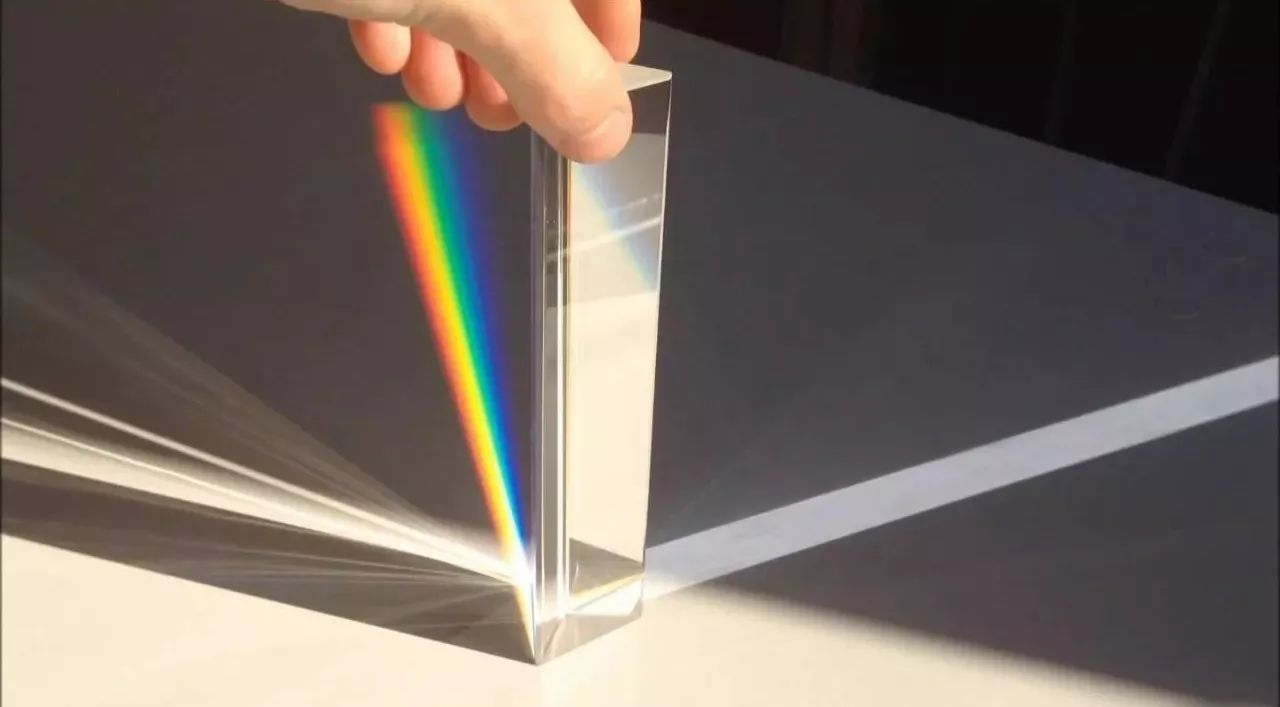
\includegraphics[width=\linewidth]{chap05/dispersion.jpg}
\end{marginfigure}
和\keyindex{干涉}{interference}{}\sidenote{译者注:经典的双缝干涉实验。}
\begin{marginfigure}
    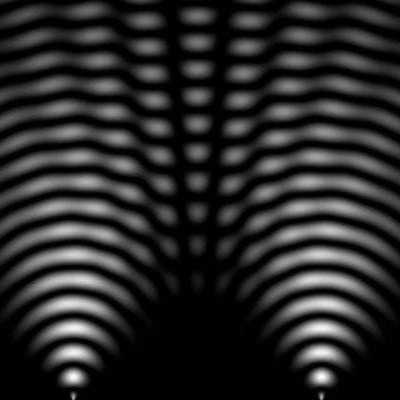
\includegraphics[width=\linewidth]{chap05/interference.jpg}
\end{marginfigure}
等效应建模。
在更精细的细节层面上,需要\keyindex{量子力学}{quantum mechanics}{}来描述光与原子的交互。
幸运的是,解决计算机图形学中的渲染问题不用直接模拟量子力学原理,
故避免了此类方法的复杂性。

在pbrt中,我们将假设几何光学是足够用来描述光与光散射的模型。
这导出了一些整个系统中隐含使用的关于光的行为的基本假设:
\begin{itemize}
    \item \keyindex{线性关系}{linearity}{}:光学系统两个输入的共同效应总是等于每个输入各自效应之和。
    \item \keyindex{能量守恒}{conservation of energy}{}\sidenote{译者注:原文写作energy conservation。}:
    当光从表面或介质散射时,触发的散射不会比它开始时产生更多的能量。
    \item {\sffamily 无偏振}:我们将忽略电磁场的偏振;
    因此,光的唯一相关属性是它关于波长(或等价地,\keyindex{频率}{frequency}{})的分布。
    \item {\sffamily 无}\keyindex{荧光}{fluorescence}{}或\keyindex{磷光}{phosphorescence}{}:
    某一波长的光的行为完全独立于其他波长或时间的光的行为。
    像偏振那样,要包含这些效应并不难,但它们为系统增加的实用价值相对较低。
    \item \keyindex{稳态}{steady state}{}:假设环境中的光达到平衡,
    所以其辐射分布不随时间变化。在现实场景中这对于光几乎是一瞬间发生的,
    所以在实践中这没什么限制。注意磷光也违反了稳态假设。
\end{itemize}

采用几何光学模型最明显的损失是很难考虑\keyindex{衍射}{diffraction}{}和干涉效应。
如\citet[p. 24]{PREISENDORFER19653}所述,这是个很难解决的问题,
例如,当存在这些效应时两区域的总通量不一定等于每个区域各自接收的功率之和。

\subsection{基本量}\label{sub:基本量}
有四个辐射度量数量\sidenote{译者注:依据中国国家标准GB 3102.6-93,
这些量的名称大都可以省略“射”字,例如“辐射出射度”也可以称作
“辐射出度”“辐出射度”“辐出度”,以此类推。后续译文将视情况使用全称或简称。}
是渲染的核心:\keyindex{通量}{flux}{}、
\keyindex{辐射照度}{irradiance}{}/\keyindex{辐射出射度}{radiant exitance}{}、
\keyindex{强度}{intensity}{}和\keyindex{辐射亮度}{radiance}{}。
它们每个都可以从能量(单位为焦耳)依次对时间、面积和方向取极限推导出来。
所有这些辐射度量数量一般都依赖于波长。
对于本章的剩余部分,我们不再明确这一依赖关系,但记住这一性质是很重要的。

\subsubsection*{能量}
我们的起点是\keyindex{能量}{energy}{}
\sidenote{译者注:也称为\keyindex{辐射能}{radiant energy}{}。},
单位为\keyindex{焦耳}{joule}{}(焦,J)
\sidenote{译者注:{\normalfont $1\text{J}=1\text{kg}\cdot\text{m}^2/\text{s}^2$。}}。
照射源发射\keyindex{光子}{photon}{},
每个光子有特定波长并携带特定数量的能量。
所有这些基本辐射度量数量实际都是对光子的不同度量。
波长为$\lambda$的一个光子携带能量为
\begin{align*}
    Q=\frac{hc}{\lambda}\, ,
\end{align*}
其中$c$是光的速率
\sidenote{译者注:指真空环境下的光速;
原文写作{\normalfont $299,472,458\text{m}/\text{s}$},此处更正为国际标准值。}
即$299,792,458\text{m}/\text{s}$,$h$为\keyindex{普朗克常数}{Planck constant}{}
\sidenote{译者注:其单位可化简为{\normalfont$\text{J}\cdot\text{s}$}。},
$h\approx6.626\times10^{-34}\text{kg}\cdot\text{m}^2/\text{s}$。

\subsubsection*{通量}
能量度量了一段时间上的\keyindex{功}{work}{},
尽管渲染一般使用稳态假设,但我们最感兴趣的是度量一瞬间的光。
\keyindex{辐射能通量}{radiant energy flux}{}
\sidenote{译者注:也称辐射通量、辐通量;原文写作radiant flux。},
也称为\keyindex{辐射功率}{radiant power}{}\sidenote{译者注:原文写作power。},
是单位时间内穿过表面或空间区域的能量总量。
辐射通量可以通过求每个微分时间内微分能量的极限算出:
\begin{align*}
    \varPhi=\lim\limits_{\Delta t\rightarrow 0}{\frac{\Delta Q}{\Delta t}}=\frac{\mathrm{d}Q}{\mathrm{d}t}\, .
\end{align*}
它的单位是焦耳$/$秒,即更常见的\keyindex{瓦特}{watt}{}(瓦,W)。

例如,设一光源在一小时内发射了$Q=200,000\text{J}$,
如果这一小时内任何时候发射的能量都相同,
我们可以求得该光源的通量为
\begin{align*}
    \varPhi=200,000\text{J}/3600\text{s}\approx 55.6\text{W}\, .
\end{align*}

反之,设通量是时间的函数,我们可以在一段时间上积分算出总能量:
\begin{align*}
    Q=\int_{t_0}^{t_1}\varPhi(t)\mathrm{d}t\, .
\end{align*}

注意这里我们的记号有些不正式:在其他问题中,因为光子实际上是离散量子,
对趋近于零的微分时间取极限没有实际意义。
但对于渲染目的,光子数量相比于我们感兴趣的度量是巨大的,在实践中这一细节不会有问题。

来自光源的总辐射一般用通量描述。
\reffig{5.6}展示了来自一个点光源的通量由
穿过包围该光源的假想球面的能量总量度量。
注意\reffig{5.6}中在两个球面的任意一个上度量的通量总量是一样的——
尽管穿过大球任意局部的能量比小球少,
但大球的面积更大,意味着总通量一样多。
\begin{figure}[htbp]
    \centering%LaTeX with PSTricks extensions
%%Creator: Inkscape 1.0.1 (3bc2e813f5, 2020-09-07)
%%Please note this file requires PSTricks extensions
\psset{xunit=.5pt,yunit=.5pt,runit=.5pt}
\begin{pspicture}(254.8999939,254.8999939)
{
\newrgbcolor{curcolor}{0 0 0}
\pscustom[linewidth=1,linecolor=curcolor]
{
\newpath
\moveto(188.40000153,127.20999146)
\curveto(188.40000153,151.66779751)(173.6668771,173.71750129)(151.07121577,183.07656872)
\curveto(128.47560051,192.43561706)(102.46763049,187.26077332)(85.17342447,169.96656729)
\curveto(67.87921844,152.67236127)(62.7043747,126.66439125)(72.06342304,104.06877599)
\curveto(81.42249047,81.47311466)(103.47219425,66.73999023)(127.93000031,66.73999023)
\curveto(152.38780636,66.73999023)(174.43751014,81.47311466)(183.79657757,104.06877599)
\curveto(193.15562591,126.66439125)(187.98078217,152.67236127)(170.68657615,169.96656729)
\curveto(153.39237012,187.26077332)(127.3844001,192.43561706)(104.78878484,183.07656872)
\curveto(82.19312351,173.71750129)(67.45999908,151.66779751)(67.45999908,127.20999146)
\curveto(67.45999908,102.7521854)(82.19312351,80.70248162)(104.78878484,71.34341419)
\curveto(127.3844001,61.98436585)(153.39237012,67.15920959)(170.68657615,84.45341562)
\curveto(187.98078217,101.74762164)(193.15562591,127.75559166)(183.79657757,150.35120692)
\curveto(174.43751014,172.94686825)(152.38780636,187.67999268)(127.93000031,187.67999268)
\curveto(103.47219425,187.67999268)(81.42249047,172.94686825)(72.06342304,150.35120692)
\curveto(62.7043747,127.75559166)(67.87921844,101.74762164)(85.17342447,84.45341562)
\curveto(102.46763049,67.15920959)(128.47560051,61.98436585)(151.07121577,71.34341419)
\curveto(173.6668771,80.70248162)(188.40000153,102.7521854)(188.40000153,127.20999146)
\closepath
}
}
{
\newrgbcolor{curcolor}{0 0 0}
\pscustom[linewidth=1,linecolor=curcolor]
{
\newpath
\moveto(254.3999939,127.44999695)
\curveto(254.3999939,178.7964223)(223.46944879,225.08730657)(176.03238777,244.73562073)
\curveto(128.59542349,264.38389481)(73.99460246,253.5198898)(37.68735328,217.21264062)
\curveto(1.3801041,180.90539144)(-9.48390091,126.30457041)(10.16437317,78.86760613)
\curveto(29.81268733,31.43054511)(76.1035716,0.5)(127.44999695,0.5)
\curveto(178.7964223,0.5)(225.08730657,31.43054511)(244.73562073,78.86760613)
\curveto(264.38389481,126.30457041)(253.5198898,180.90539144)(217.21264062,217.21264062)
\curveto(180.90539144,253.5198898)(126.30457041,264.38389481)(78.86760613,244.73562073)
\curveto(31.43054511,225.08730657)(0.5,178.7964223)(0.5,127.44999695)
\curveto(0.5,76.1035716)(31.43054511,29.81268733)(78.86760613,10.16437317)
\curveto(126.30457041,-9.48390091)(180.90539144,1.3801041)(217.21264062,37.68735328)
\curveto(253.5198898,73.99460246)(264.38389481,128.59542349)(244.73562073,176.03238777)
\curveto(225.08730657,223.46944879)(178.7964223,254.3999939)(127.44999695,254.3999939)
\curveto(76.1035716,254.3999939)(29.81268733,223.46944879)(10.16437317,176.03238777)
\curveto(-9.48390091,128.59542349)(1.3801041,73.99460246)(37.68735328,37.68735328)
\curveto(73.99460246,1.3801041)(128.59542349,-9.48390091)(176.03238777,10.16437317)
\curveto(223.46944879,29.81268733)(254.3999939,76.1035716)(254.3999939,127.44999695)
\closepath
}
}
{
\newrgbcolor{curcolor}{0.98823529 0.93333334 0.12941177}
\pscustom[linestyle=none,fillstyle=solid,fillcolor=curcolor]
{
\newpath
\moveto(132.21,146.9699939)
\lineto(130.63,137.2899939)
\lineto(135.58,145.7499939)
\lineto(132.25,136.5299939)
\lineto(138.67,143.9399939)
\lineto(133.71,135.4899939)
\lineto(141.38,141.5799939)
\lineto(134.95,134.1899939)
\lineto(143.61,138.7699939)
\lineto(135.93,132.6899939)
\lineto(145.29,135.5999939)
\lineto(136.62,131.0299939)
\lineto(146.35,132.1799939)
\lineto(136.99,129.2799939)
\lineto(146.77,128.6099939)
\lineto(137.03,127.4799939)
\lineto(146.52,125.0399939)
\lineto(136.74,125.7099939)
\lineto(145.62,121.5599939)
\lineto(136.14,124.0299939)
\lineto(144.1,118.3099939)
\lineto(135.23,122.4799939)
\lineto(142.01,115.3999939)
\lineto(134.05,121.1299939)
\lineto(139.42,112.9199939)
\lineto(132.65,120.0099939)
\lineto(136.41,110.9599939)
\lineto(131.06,119.1699939)
\lineto(133.1,109.5899939)
\lineto(129.35,118.6399939)
\lineto(129.59,108.8399939)
\lineto(127.57,118.4299939)
\lineto(126,108.7599939)
\lineto(125.78,118.5599939)
\lineto(122.47,109.3299939)
\lineto(124.04,118.9999939)
\lineto(119.09,110.5499939)
\lineto(122.42,119.7699939)
\lineto(116,112.3599939)
\lineto(120.96,120.8099939)
\lineto(113.29,114.7099939)
\lineto(119.72,122.1099939)
\lineto(111.06,117.5199939)
\lineto(118.74,123.6099939)
\lineto(109.38,120.6999939)
\lineto(118.05,125.2699939)
\lineto(108.32,124.1199939)
\lineto(117.68,127.0199939)
\lineto(107.9,127.6799939)
\lineto(117.64,128.8099939)
\lineto(108.15,131.2599939)
\lineto(117.93,130.5799939)
\lineto(109.05,134.7299939)
\lineto(118.53,132.2699939)
\lineto(110.57,137.9799939)
\lineto(119.44,133.8199939)
\lineto(112.66,140.8999939)
\lineto(120.62,135.1699939)
\lineto(115.25,143.3699939)
\lineto(122.02,136.2899939)
\lineto(118.26,145.3399939)
\lineto(123.61,137.1199939)
\lineto(121.57,146.7099939)
\lineto(125.32,137.6599939)
\lineto(125.08,147.4599939)
\lineto(127.1,137.8699939)
\lineto(128.66,147.5399939)
\lineto(128.89,137.7399939)
\closepath
}
}
{
\newrgbcolor{curcolor}{0 0 0}
\pscustom[linewidth=0.30000001,linecolor=curcolor]
{
\newpath
\moveto(132.21,146.9699939)
\lineto(130.63,137.2899939)
\lineto(135.58,145.7499939)
\lineto(132.25,136.5299939)
\lineto(138.67,143.9399939)
\lineto(133.71,135.4899939)
\lineto(141.38,141.5799939)
\lineto(134.95,134.1899939)
\lineto(143.61,138.7699939)
\lineto(135.93,132.6899939)
\lineto(145.29,135.5999939)
\lineto(136.62,131.0299939)
\lineto(146.35,132.1799939)
\lineto(136.99,129.2799939)
\lineto(146.77,128.6099939)
\lineto(137.03,127.4799939)
\lineto(146.52,125.0399939)
\lineto(136.74,125.7099939)
\lineto(145.62,121.5599939)
\lineto(136.14,124.0299939)
\lineto(144.1,118.3099939)
\lineto(135.23,122.4799939)
\lineto(142.01,115.3999939)
\lineto(134.05,121.1299939)
\lineto(139.42,112.9199939)
\lineto(132.65,120.0099939)
\lineto(136.41,110.9599939)
\lineto(131.06,119.1699939)
\lineto(133.1,109.5899939)
\lineto(129.35,118.6399939)
\lineto(129.59,108.8399939)
\lineto(127.57,118.4299939)
\lineto(126,108.7599939)
\lineto(125.78,118.5599939)
\lineto(122.47,109.3299939)
\lineto(124.04,118.9999939)
\lineto(119.09,110.5499939)
\lineto(122.42,119.7699939)
\lineto(116,112.3599939)
\lineto(120.96,120.8099939)
\lineto(113.29,114.7099939)
\lineto(119.72,122.1099939)
\lineto(111.06,117.5199939)
\lineto(118.74,123.6099939)
\lineto(109.38,120.6999939)
\lineto(118.05,125.2699939)
\lineto(108.32,124.1199939)
\lineto(117.68,127.0199939)
\lineto(107.9,127.6799939)
\lineto(117.64,128.8099939)
\lineto(108.15,131.2599939)
\lineto(117.93,130.5799939)
\lineto(109.05,134.7299939)
\lineto(118.53,132.2699939)
\lineto(110.57,137.9799939)
\lineto(119.44,133.8199939)
\lineto(112.66,140.8999939)
\lineto(120.62,135.1699939)
\lineto(115.25,143.3699939)
\lineto(122.02,136.2899939)
\lineto(118.26,145.3399939)
\lineto(123.61,137.1199939)
\lineto(121.57,146.7099939)
\lineto(125.32,137.6599939)
\lineto(125.08,147.4599939)
\lineto(127.1,137.8699939)
\lineto(128.66,147.5399939)
\lineto(128.89,137.7399939)
\closepath
}
}
{
\newrgbcolor{curcolor}{0 0 0}
\pscustom[linewidth=1,linecolor=curcolor]
{
\newpath
\moveto(127.12999725,173.73999023)
\lineto(127.12999725,153.51999664)
}
}
{
\newrgbcolor{curcolor}{0 0 0}
\pscustom[linestyle=none,fillstyle=solid,fillcolor=curcolor]
{
\newpath
\moveto(121.63,168.8399939)
\lineto(127.13,173.0899939)
\lineto(132.63,168.8399939)
\lineto(127.13,181.8499939)
\closepath
}
}
{
\newrgbcolor{curcolor}{0.65098041 0.65098041 0.65098041}
\pscustom[linestyle=none,fillstyle=solid,fillcolor=curcolor]
{
\newpath
\moveto(122.83,170.3899939)
\lineto(127.13,180.5399939)
\lineto(127.13,173.7299939)
\closepath
}
}
{
\newrgbcolor{curcolor}{0.40000001 0.40000001 0.40000001}
\pscustom[linestyle=none,fillstyle=solid,fillcolor=curcolor]
{
\newpath
\moveto(131.43,170.3899939)
\lineto(127.13,180.5399939)
\lineto(127.13,173.7299939)
\closepath
}
}
{
\newrgbcolor{curcolor}{0 0 0}
\pscustom[linewidth=1,linecolor=curcolor]
{
\newpath
\moveto(127.12999725,233.55999374)
\lineto(127.12999725,198.08999252)
}
}
{
\newrgbcolor{curcolor}{0 0 0}
\pscustom[linestyle=none,fillstyle=solid,fillcolor=curcolor]
{
\newpath
\moveto(121.63,228.6499939)
\lineto(127.13,232.9099939)
\lineto(132.63,228.6499939)
\lineto(127.13,241.6699939)
\closepath
}
}
{
\newrgbcolor{curcolor}{0.65098041 0.65098041 0.65098041}
\pscustom[linestyle=none,fillstyle=solid,fillcolor=curcolor]
{
\newpath
\moveto(122.83,230.2099939)
\lineto(127.13,240.3499939)
\lineto(127.13,233.5399939)
\closepath
}
}
{
\newrgbcolor{curcolor}{0.40000001 0.40000001 0.40000001}
\pscustom[linestyle=none,fillstyle=solid,fillcolor=curcolor]
{
\newpath
\moveto(131.43,230.2099939)
\lineto(127.13,240.3499939)
\lineto(127.13,233.5399939)
\closepath
}
}
{
\newrgbcolor{curcolor}{0 0 0}
\pscustom[linewidth=1,linecolor=curcolor]
{
\newpath
\moveto(107.52999878,169.63999176)
\lineto(116.30000305,151.42999268)
}
}
{
\newrgbcolor{curcolor}{0 0 0}
\pscustom[linestyle=none,fillstyle=solid,fillcolor=curcolor]
{
\newpath
\moveto(104.7,162.8299939)
\lineto(107.81,169.0599939)
\lineto(114.62,167.6099939)
\lineto(104.01,176.9499939)
\closepath
}
}
{
\newrgbcolor{curcolor}{0.65098041 0.65098041 0.65098041}
\pscustom[linestyle=none,fillstyle=solid,fillcolor=curcolor]
{
\newpath
\moveto(105.11,164.7599939)
\lineto(104.58,175.7599939)
\lineto(107.54,169.6299939)
\closepath
}
}
{
\newrgbcolor{curcolor}{0.40000001 0.40000001 0.40000001}
\pscustom[linestyle=none,fillstyle=solid,fillcolor=curcolor]
{
\newpath
\moveto(112.85,168.4899939)
\lineto(104.58,175.7599939)
\lineto(107.54,169.6299939)
\closepath
}
}
{
\newrgbcolor{curcolor}{0 0 0}
\pscustom[linewidth=1,linecolor=curcolor]
{
\newpath
\moveto(81.55999756,223.53999329)
\lineto(96.95999908,191.5799942)
}
}
{
\newrgbcolor{curcolor}{0 0 0}
\pscustom[linestyle=none,fillstyle=solid,fillcolor=curcolor]
{
\newpath
\moveto(78.74,216.7199939)
\lineto(81.85,222.9499939)
\lineto(88.65,221.4999939)
\lineto(78.05,230.8299939)
\closepath
}
}
{
\newrgbcolor{curcolor}{0.65098041 0.65098041 0.65098041}
\pscustom[linestyle=none,fillstyle=solid,fillcolor=curcolor]
{
\newpath
\moveto(79.14,218.6499939)
\lineto(78.62,229.6499939)
\lineto(81.57,223.5199939)
\closepath
}
}
{
\newrgbcolor{curcolor}{0.40000001 0.40000001 0.40000001}
\pscustom[linestyle=none,fillstyle=solid,fillcolor=curcolor]
{
\newpath
\moveto(86.89,222.3799939)
\lineto(78.62,229.6499939)
\lineto(81.57,223.5199939)
\closepath
}
}
{
\newrgbcolor{curcolor}{0 0 0}
\pscustom[linewidth=1,linecolor=curcolor]
{
\newpath
\moveto(92.12999725,156.56999207)
\lineto(107.69999695,143.66999054)
}
}
{
\newrgbcolor{curcolor}{0 0 0}
\pscustom[linestyle=none,fillstyle=solid,fillcolor=curcolor]
{
\newpath
\moveto(92.4,149.1999939)
\lineto(92.63,156.1599939)
\lineto(99.42,157.6799939)
\lineto(85.89,161.7399939)
\closepath
}
}
{
\newrgbcolor{curcolor}{0.65098041 0.65098041 0.65098041}
\pscustom[linestyle=none,fillstyle=solid,fillcolor=curcolor]
{
\newpath
\moveto(91.97,151.1199939)
\lineto(86.9,160.9099939)
\lineto(92.15,156.5599939)
\closepath
}
}
{
\newrgbcolor{curcolor}{0.40000001 0.40000001 0.40000001}
\pscustom[linestyle=none,fillstyle=solid,fillcolor=curcolor]
{
\newpath
\moveto(97.45,157.7399939)
\lineto(86.9,160.9099939)
\lineto(92.15,156.5599939)
\closepath
}
}
{
\newrgbcolor{curcolor}{0 0 0}
\pscustom[linewidth=1,linecolor=curcolor]
{
\newpath
\moveto(46.06999969,194.73999405)
\lineto(73.38999939,172.10999298)
}
}
{
\newrgbcolor{curcolor}{0 0 0}
\pscustom[linestyle=none,fillstyle=solid,fillcolor=curcolor]
{
\newpath
\moveto(46.34,187.3699939)
\lineto(46.57,194.3299939)
\lineto(53.37,195.8499939)
\lineto(39.83,199.9199939)
\closepath
}
}
{
\newrgbcolor{curcolor}{0.65098041 0.65098041 0.65098041}
\pscustom[linestyle=none,fillstyle=solid,fillcolor=curcolor]
{
\newpath
\moveto(45.91,189.2899939)
\lineto(40.84,199.0799939)
\lineto(46.09,194.7299939)
\closepath
}
}
{
\newrgbcolor{curcolor}{0.40000001 0.40000001 0.40000001}
\pscustom[linestyle=none,fillstyle=solid,fillcolor=curcolor]
{
\newpath
\moveto(51.4,195.9099939)
\lineto(40.84,199.0799939)
\lineto(46.09,194.7299939)
\closepath
}
}
{
\newrgbcolor{curcolor}{0 0 0}
\pscustom[linewidth=1,linecolor=curcolor]
{
\newpath
\moveto(147.63000488,169.3299942)
\lineto(138.8500061,151.11999512)
}
}
{
\newrgbcolor{curcolor}{0 0 0}
\pscustom[linestyle=none,fillstyle=solid,fillcolor=curcolor]
{
\newpath
\moveto(140.54,167.2999939)
\lineto(147.34,168.7499939)
\lineto(150.45,162.5199939)
\lineto(151.14,176.6299939)
\closepath
}
}
{
\newrgbcolor{curcolor}{0.65098041 0.65098041 0.65098041}
\pscustom[linestyle=none,fillstyle=solid,fillcolor=curcolor]
{
\newpath
\moveto(142.3,168.1799939)
\lineto(150.57,175.4499939)
\lineto(147.62,169.3199939)
\closepath
}
}
{
\newrgbcolor{curcolor}{0.40000001 0.40000001 0.40000001}
\pscustom[linestyle=none,fillstyle=solid,fillcolor=curcolor]
{
\newpath
\moveto(150.04,164.4499939)
\lineto(150.57,175.4499939)
\lineto(147.62,169.3199939)
\closepath
}
}
{
\newrgbcolor{curcolor}{0 0 0}
\pscustom[linewidth=1,linecolor=curcolor]
{
\newpath
\moveto(173.58999634,223.21999359)
\lineto(158.19000244,191.26999283)
}
}
{
\newrgbcolor{curcolor}{0 0 0}
\pscustom[linestyle=none,fillstyle=solid,fillcolor=curcolor]
{
\newpath
\moveto(166.5,221.1899939)
\lineto(173.31,222.6399939)
\lineto(176.42,216.4099939)
\lineto(177.11,230.5199939)
\closepath
}
}
{
\newrgbcolor{curcolor}{0.65098041 0.65098041 0.65098041}
\pscustom[linestyle=none,fillstyle=solid,fillcolor=curcolor]
{
\newpath
\moveto(168.26,222.0699939)
\lineto(176.54,229.3399939)
\lineto(173.58,223.2099939)
\closepath
}
}
{
\newrgbcolor{curcolor}{0.40000001 0.40000001 0.40000001}
\pscustom[linestyle=none,fillstyle=solid,fillcolor=curcolor]
{
\newpath
\moveto(176.01,218.3399939)
\lineto(176.54,229.3399939)
\lineto(173.58,223.2099939)
\closepath
}
}
{
\newrgbcolor{curcolor}{0 0 0}
\pscustom[linewidth=1,linecolor=curcolor]
{
\newpath
\moveto(163.02000427,156.25999451)
\lineto(147.44999695,143.35999298)
}
}
{
\newrgbcolor{curcolor}{0 0 0}
\pscustom[linestyle=none,fillstyle=solid,fillcolor=curcolor]
{
\newpath
\moveto(155.73,157.3699939)
\lineto(162.52,155.8499939)
\lineto(162.75,148.8899939)
\lineto(169.26,161.4299939)
\closepath
}
}
{
\newrgbcolor{curcolor}{0.65098041 0.65098041 0.65098041}
\pscustom[linestyle=none,fillstyle=solid,fillcolor=curcolor]
{
\newpath
\moveto(157.7,157.4399939)
\lineto(168.25,160.5999939)
\lineto(163.01,156.2499939)
\closepath
}
}
{
\newrgbcolor{curcolor}{0.40000001 0.40000001 0.40000001}
\pscustom[linestyle=none,fillstyle=solid,fillcolor=curcolor]
{
\newpath
\moveto(163.18,150.8199939)
\lineto(168.25,160.5999939)
\lineto(163.01,156.2499939)
\closepath
}
}
{
\newrgbcolor{curcolor}{0 0 0}
\pscustom[linewidth=1,linecolor=curcolor]
{
\newpath
\moveto(209.08000183,194.42999268)
\lineto(181.77000427,171.79999542)
}
}
{
\newrgbcolor{curcolor}{0 0 0}
\pscustom[linestyle=none,fillstyle=solid,fillcolor=curcolor]
{
\newpath
\moveto(201.79,195.5399939)
\lineto(208.58,194.0199939)
\lineto(208.81,187.0599939)
\lineto(215.32,199.5999939)
\closepath
}
}
{
\newrgbcolor{curcolor}{0.65098041 0.65098041 0.65098041}
\pscustom[linestyle=none,fillstyle=solid,fillcolor=curcolor]
{
\newpath
\moveto(203.75,195.6099939)
\lineto(214.31,198.7699939)
\lineto(209.06,194.4199939)
\closepath
}
}
{
\newrgbcolor{curcolor}{0.40000001 0.40000001 0.40000001}
\pscustom[linestyle=none,fillstyle=solid,fillcolor=curcolor]
{
\newpath
\moveto(209.24,188.9799939)
\lineto(214.31,198.7699939)
\lineto(209.06,194.4199939)
\closepath
}
}
\end{pspicture}

    \caption{辐射通量$\varPhi$度量穿过表面或空间区域的能量。
    这里来自一个点光源的通量由包围它的球来度量。}
    \label{fig:5.6}
\end{figure}

\subsubsection*{辐射照度与辐射出射度}

\subsection{亮度和光度学}\label{sub:亮度和光度学}

\section{处理辐射积分}\label{sec:处理辐射积分}

渲染中最频繁的任务之一就是求辐射度量数量的积分。
本节中,我们将介绍可以使该任务更简单的一些技巧。
为了说明这些技术的运用,我们将以计算在一点处的辐射照度为例。
在曲面法线为$\bm n$的点$\bm p$处的辐射照度取决于
方向集$\Omega$上的辐射亮度即
\begin{align}\label{eq:5.4}
    E({\bm p},{\bm n})=\int\limits_{\Omega}{L_{\mathrm{i}}({\bm p},{\bm\omega})|\cos\theta|\mathrm{d}\bm\omega}\, ,
\end{align}
其中$L_{\mathrm{i}}({\bm p},{\bm\omega})$是入射辐亮度函数(\reffig{5.12})
而该积分中项$\cos\theta$取决于辐射亮度定义中的项$\mathrm{d}A^{\perp}$。
$\theta$度量$\bm\omega$和曲面法线$\bm n$之间的夹角。
辐射照度通常在关于给定曲面法线$\bm n$的半球方向$H^2(\bm n)$上算出。
\begin{figure}[htbp]
    \centering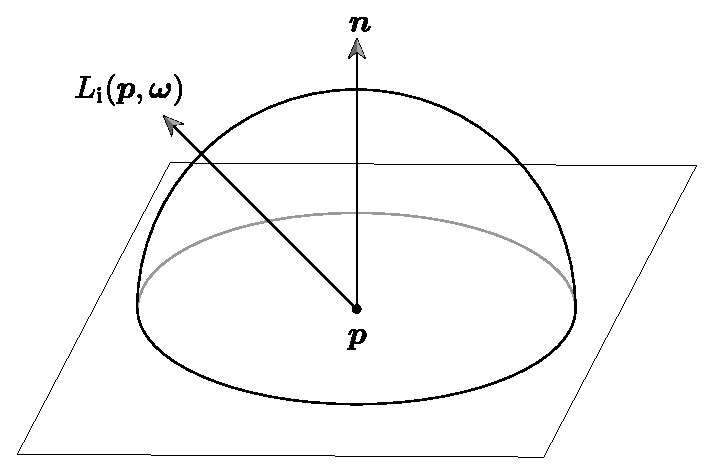
\includegraphics[width=0.5\linewidth]{chap05/Irradiancefromradiance.eps}
    \caption{点$\bm p$处的辐射照度由辐射亮度乘以在该点上整个上半球入射方向余弦的积分得到。}
    \label{fig:5.12}
\end{figure}

\subsection{投影立体角上的积分}\label{sub:投影立体角上的积分}
辐射度量数量积分中的各种余弦常常和积分学中的解释搞混。
度量积分所需的物体所对面积时这个问题可通过
用\keyindex{投影立体角}{projected solid angle}{solid angle立体角}而不用立体角来避免。
物体所对的投影立体角通过将该物体投影到单位球上决定,
这和立体角的做法一样,但接着要将所得形状再向下投影到
垂直于曲面法线的单位圆盘上(\reffig{5.13})。
半球方向上关于余弦加权的立体角积分可重写为在投影立体角上的积分。
\begin{figure}[htbp]
    \centering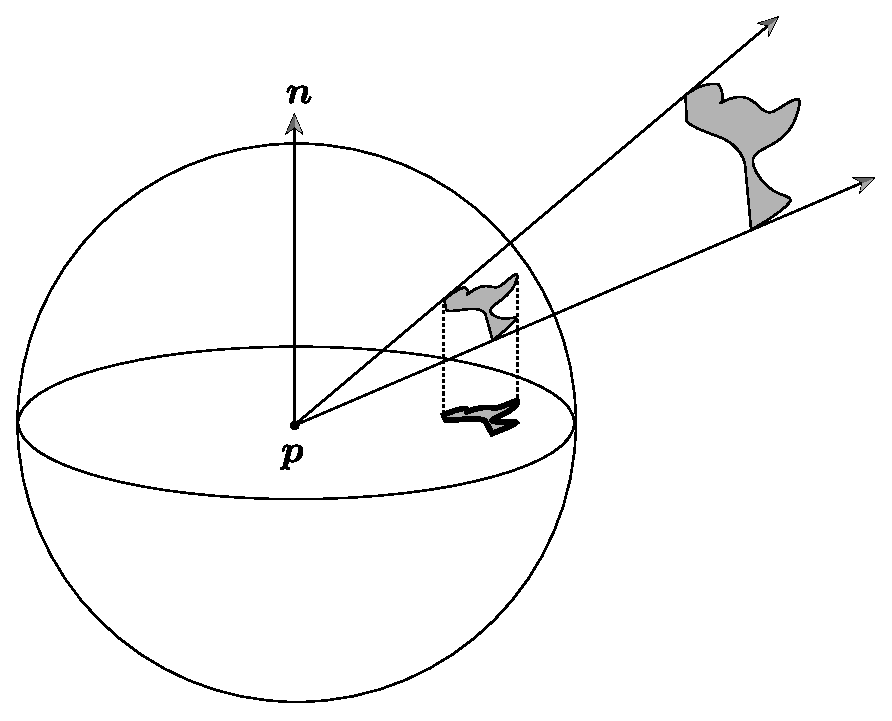
\includegraphics[width=0.6\linewidth]{chap05/Projectedsolidangle.eps}
    \caption{物体所对的投影立体角是其所对的余弦加权立体角。
        通过求物体的立体角、将其向下投影到垂直于曲面法线的平面上并
        度量该区域的面积可以将其算出。因此投影立体角取决于
        计算处的曲面法线,因为法线朝着平面投影方向。}
    \label{fig:5.13}
\end{figure}

投影立体角度量与立体角度量的关系为
\begin{align*}
    \mathrm{d}{\bm\omega}^{\perp}=|\cos\theta|\mathrm{d}{\bm\omega}\, ,
\end{align*}
所以在半球上由辐射亮度计算辐射照度的积分可更简单地重写为
\begin{align*}
    E({\bm p},{\bm n})=\int\limits_{H^2({\bm n})}{L_{\mathrm{i}}({\bm p},{\bm\omega})\mathrm{d}{\bm\omega}^{\perp}}\, .
\end{align*}

对于本书剩余部分,我们会以立体角而不是投影立体角的形式书写方向上的积分。
然而在其他资源中,可能会用投影立体角,所以弄清被积分式实际的度量总是很重要的。

正如我们用入射辐亮度求辐射照度那样,我们也可以通过在物体表面积$A$上积分
来计算从某物体向法线周围半球发出的总通量:
\begin{align*}
    \varPhi & =\int\limits_A{\int\limits_{H^2({\bm n})}L_{\mathrm{o}}({\bm p},{\bm\omega})\cos\theta\mathrm{d}{\bm\omega}\mathrm{d}A}   \\
            & =\int\limits_A{\int\limits_{H^2({\bm n})}L_{\mathrm{o}}({\bm p},{\bm\omega})\mathrm{d}{\bm\omega}^{\perp}\mathrm{d}A}\, .
\end{align*}

\subsection{球坐标上的积分}\label{sub:球坐标上的积分}
将立体角上的积分转化到球面坐标$(\theta,\varphi)$上常常很方便。
回想一个$(x,y,z)$方向坐标也可写成球面角形式(\reffig{5.14})
\sidenote{译者注:原书此图和后续图中标注为$\varphi$,该公式和后续公式则使用$\phi$。
    笔者修改为统一使用$\varphi$,与前面的章节照应。}:
\begin{align*}
    x & =\sin\theta\cos\varphi\, , \\
    y & =\sin\theta\sin\varphi\, , \\
    z & =\cos\theta\, .
\end{align*}
\begin{figure}[htbp]
    \centering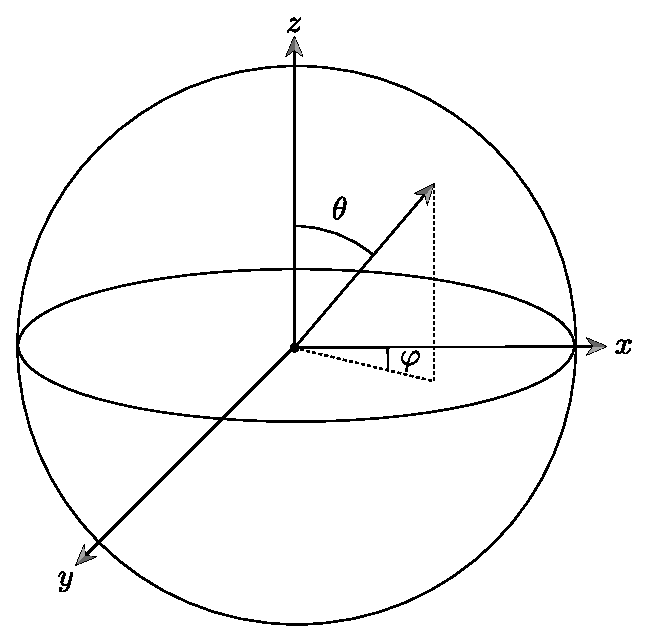
\includegraphics[width=0.5\linewidth]{chap05/Sphericalcoordinates.eps}
    \caption{如果也给出了基向量$x,y$和$z$,则方向向量也可写作球面坐标$(\theta,\varphi)$的形式。
        球面角公式让两者之间的转化很容易。}
    \label{fig:5.14}
\end{figure}

为了将立体角上的积分转化为$(\theta,\varphi)$上的积分,
我们需要能表达方向集的微分面积$\mathrm{d}\bm\omega$
与$(\theta,\varphi)$的微分面积之间的关系(\reffig{5.15})。
微分面积$\mathrm{d}\bm\omega$是其边的
微分长度$\sin\theta\mathrm{d}\varphi$和$\mathrm{d}\theta$之积。因此,
\begin{align}\label{eq:5.5}
    \mathrm{d}{\bm\omega}=\sin\theta\mathrm{d}\theta\mathrm{d}\varphi\, .
\end{align}
\begin{figure}[htbp]
    \centering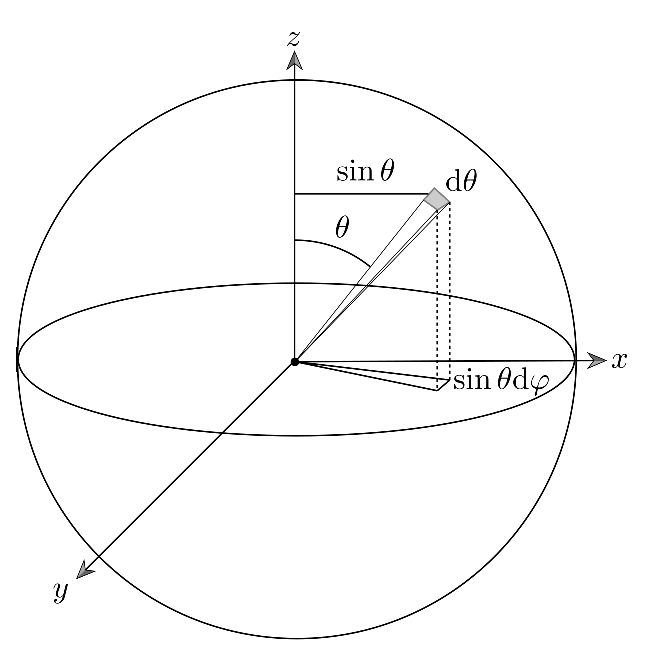
\includegraphics[width=0.5\linewidth]{chap05/Sindthetadphi.eps}
    \caption{一个微分立体角所对的微分面积$\mathrm{d}\bm\omega$是
        两边微分长度$\sin\theta\mathrm{d}\varphi$和$\mathrm{d}\theta$的积。
        得到的关系$\mathrm{d}{\bm\omega}=\sin\theta\mathrm{d}\theta\mathrm{d}\varphi$是
        在立体角上的积分和球面角上的积分之间转化的关键。}
    \label{fig:5.15}
\end{figure}

因此我们可以看到在半球上的辐射照度积分,即$\Omega=H^2({\bm n})$的\refeq{5.4},
可以等价地写为
\begin{align*}
    E({\bm p},{\bm n})=\int_0^{2\pi}\int_0^{\frac{\pi}{2}}L_{\mathrm{i}}({\bm p},\theta,\varphi)\cos\theta\sin\theta\mathrm{d}\theta\mathrm{d}\varphi\, .
\end{align*}
如果来自所有方向的辐射亮度都相同,则等式简化为$E=\pi L_{\mathrm{i}}$。

为了方便,我们将定义两个把$\theta$和$\varphi$转化为$(x,y,z)$方向向量的函数。
第一个函数直接应用之前的等式。注意这些函数传入的是$\theta$的正弦和余弦,而不是$\theta$本身。
这是因为调用者常常已经有$\theta$的正弦和余弦了。
然而这对于$\varphi$则不是常见情况,所以传入的是$\varphi$。
\begin{lstlisting}
`\refcode{Geometry Inline Functions}{+=}\lastnext{GeometryInlineFunctions}`
inline `\refvar{Vector3f}{}` `\initvar[SphericalDirection1]{SphericalDirection}{}`(`\refvar{Float}{}` sinTheta, 
        `\refvar{Float}{}` cosTheta, `\refvar{Float}{}` phi) {
    return `\refvar{Vector3f}{}`(sinTheta * std::cos(phi), 
                    sinTheta * std::sin(phi),
                    cosTheta);
}
\end{lstlisting}

第二个函数接收表示$x,y$和$z$轴的三个基向量并返回
在由它们定义的坐标系下相应的方向向量:
\begin{lstlisting}
`\refcode{Geometry Inline Functions}{+=}\lastnext{GeometryInlineFunctions}`
inline `\refvar{Vector3f}{}` `\initvar[SphericalDirection2]{SphericalDirection}{}`(`\refvar{Float}{}` sinTheta, `\refvar{Float}{}` cosTheta, 
        `\refvar{Float}{}` phi, const `\refvar{Vector3f}{}` &x, const `\refvar{Vector3f}{}` &y,
        const `\refvar{Vector3f}{}` &z) {
    return sinTheta * std::cos(phi) * x +
           sinTheta * std::sin(phi) * y + cosTheta * z;
}
\end{lstlisting}

方向$(x,y,z)$转化为球面坐标可求解为
\begin{align*}
    \theta  & =\arccos z\, ,          \\
    \varphi & =\arctan\frac{y}{x}\, .
\end{align*}
下面是对应函数。注意\refvar{SphericalTheta}{()}假设
向量{\ttfamily v}在传入前已经规范化了;
钳位足以避免浮点舍入误差使{\ttfamily |v.z|}稍大于1而引发{\ttfamily std::acos()}错误。
\begin{lstlisting}
`\refcode{Geometry Inline Functions}{+=}\lastnext{GeometryInlineFunctions}`
inline `\refvar{Float}{}` `\initvar{SphericalTheta}{}`(const `\refvar{Vector3f}{}` &v) {
    return std::acos(`\refvar{Clamp}{}`(v.z, -1, 1));
}
\end{lstlisting}
\begin{lstlisting}
`\refcode{Geometry Inline Functions}{+=}\lastcode{GeometryInlineFunctions}`
inline `\refvar{Float}{}` `\initvar{SphericalPhi}{}`(const `\refvar{Vector3f}{}` &v) {
    `\refvar{Float}{}` p = std::atan2(v.y, v.x);
    return (p < 0) ? (p + 2 * Pi) : p;
}
\end{lstlisting}

\subsection{面积上的积分}\label{sub:面积上的积分}
可以简化计算的最后一个积分变换是将方向上的积分变为面积上的积分。
再次考虑\refeq{5.4}中的辐射照度积分,
并想象有一个具有恒定出射辐亮度的假想四边形,
我们想计算在点$\bm p$所得的辐射照度。
将该值计算为方向上的积分并不简单,
因为给定特定方向后确定四边形在那个方向是否可见很重要。
将辐射照度计算为四边形面积上的积分则简单得多。

微分面积与(从点$\bm p$看向的)微分立体角的关系为
\begin{align}\label{eq:5.6}
    \mathrm{d}{\bm\omega}=\frac{\mathrm{d}A\cos\theta}{r^2}\, ,
\end{align}
其中$\theta$是$\mathrm{d}A$的曲面法线与到$\bm p$的向量之间的夹角,
而$r$是从$\bm p$到$\mathrm{d}A$的距离(\reffig{5.16})。
我们这里不会推导该结果,但它可以被直观理解:
如果$\mathrm{d}A$离$\bm p$的距离为1且恰好对齐垂直于$\mathrm{d}\bm\omega$,
则$\mathrm{d}{\bm\omega}=\mathrm{d}A$,$\theta=0$,进而\refeq{5.6}成立。
当$\mathrm{d}A$朝着远离$\bm p$运动,或者它旋转而不再对齐$\mathrm{d}\bm\omega$的方向,
则项$r^2$和$\cos\theta$做相应补偿以减小$\mathrm{d}\bm\omega$。
\begin{figure}[htbp]
    \centering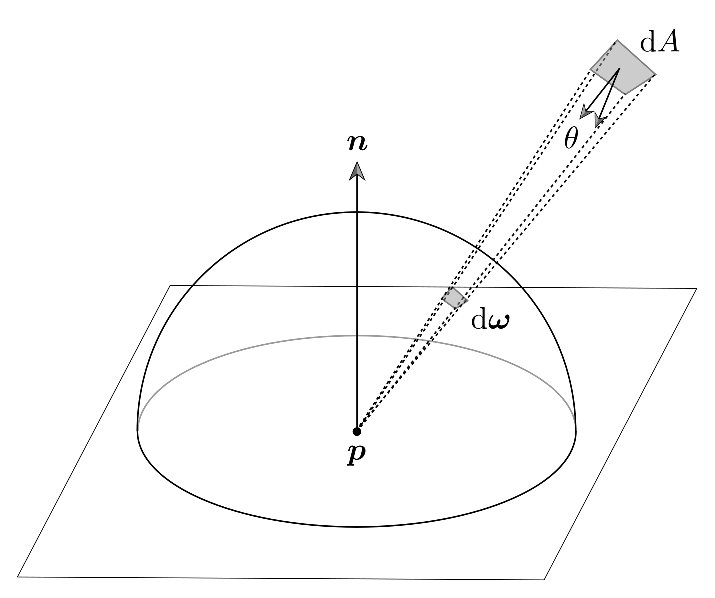
\includegraphics[width=0.5\linewidth]{chap05/DifferentialsolidangleofdA.eps}
    \caption{微分面积$\mathrm{d}A$所对的微分立体角等于$\displaystyle\frac{\mathrm{d}A\cos\theta}{r^2}$,
        其中$\theta$是$\mathrm{d}A$的曲面法线与到$\bm p$的向量之间的夹角而$r$是从$\bm p$到$\mathrm{d}A$的距离。}
    \label{fig:5.16}
\end{figure}

因此,我们可以为四边形光源写出辐射照度积分
\begin{align*}
    E({\bm p},{\bm n})=\int\limits_A L\cos\theta_{\mathrm{i}}\frac{\cos\theta_{\mathrm{o}}\mathrm{d}A}{r^2}\, ,
\end{align*}
其中$L$是发射自四边形表面的辐射亮度,$\theta_{\mathrm{i}}$是$\bm p$的
曲面法线与光路上\sidenote{译者注:原文on the light。}从$\bm p$到点$\bm p'$方向间的夹角
\sidenote{译者注:$\bm p'$是四边形上一点,原图未标出。},
而$\theta_{\mathrm{o}}$是光路上$\bm p'$的
曲面法线与从$\bm p'$到$\bm p$方向间的夹角(\reffig{5.17})。
\begin{figure}[htbp]
    \centering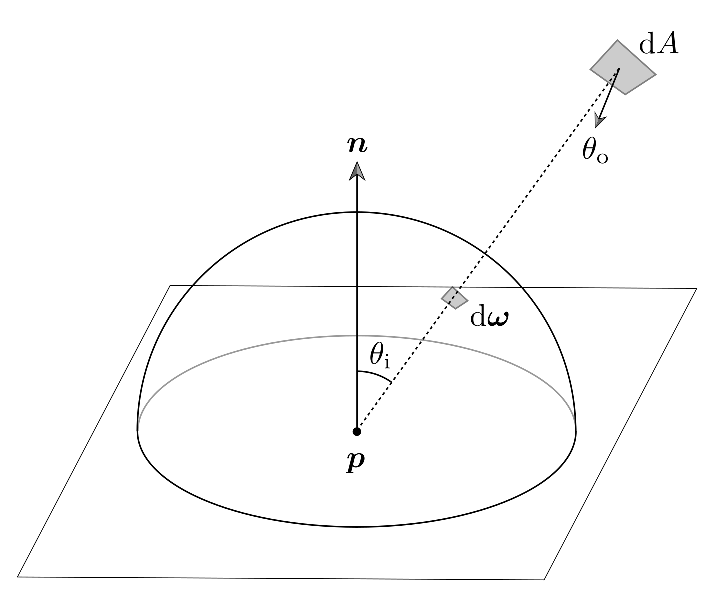
\includegraphics[width=0.5\linewidth]{chap05/Irradiancefromquadrilateral.eps}
    \caption{为了计算点$\bm p$处来自四边形光源的辐射照度,
        在光源曲面面积上积分比在其对应的不规则方向集上积分更简单。
        \refeq{5.6}给出的立体角与面积间的关系让我们在两种方法间来回切换。}
    \label{fig:5.17}
\end{figure}

\section{表面反射}\label{sec:表面反射}

当光入射到表面时,表面会散射该光,将其一部分反射回环境中。
有两个需要描述的效应以对反射建模:反射光的光谱分布和其方向分布。
例如,柠檬皮大都吸收了蓝波长的光而反射了大部分红和绿波长的光
(回想\reffig{5.1}中柠檬皮的反射SPD)。
因此,当用白光照射它时,其颜色是黄色。
无论从哪个方向观察,皮的颜色都相当一致,
但有的方向会有\keyindex{高光}{highlight}{}——会看见与其说黄色不如说白色的更亮区域
\sidenote{译者注:有高光区的柠檬照片。}。
\begin{marginfigure}
    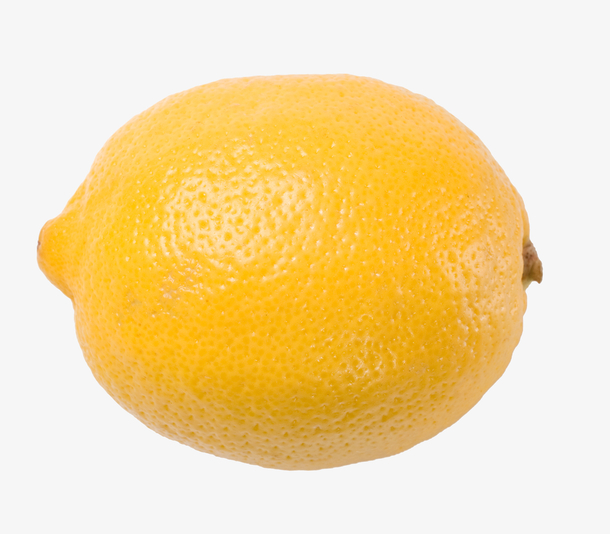
\includegraphics[width=\linewidth]{chap05/lemon.jpg}
\end{marginfigure}
相反,镜子一点反射的光几乎完全取决于观察方向。
在镜子的固定点上,当观察角度变化时,镜子反射的物体也随之变化。

来自\keyindex{半透明}{translucent}{}表面的反射更复杂;
从皮和叶子到蜡和液体的各种材料都
表现出\keyindex{次表面光传输}{subsurface light transport}{light transport光传输},
即进入表面一点的光在有一定距离的地方退出。
(例如考虑在一个人的嘴巴里开手电筒会让他的脸颊被照亮,
因为进入脸颊内侧的光穿过了皮肤并从脸上退出。)

有两种抽象来为光的反射描述这些机制:
\refsub{BRDF}和\refsub{BSSRDF}分别介绍的BRDF和BSSRDF。
BRDF描述一点的表面反射而忽略次表面光传输效应;
对于不受该传输机制明显影响的材料,
这一简化会减少报错并让渲染算法的实现高效得多。
BSSRDF推广了BRDF并描述来自半透明材料光反射的更一般设置。

\subsection{BRDF}\label{sub:BRDF}
\keyindex{双向反射分布函数}{bidirectional reflectance distribution function}{}(BRDF)
为描述来自表面的反射给出了形式。考虑\reffig{5.18}中的设置:
我们想知道,作为沿方向${\bm\omega}_{\mathrm{i}}$
入射辐亮度$L_{\mathrm{i}}({\bm p},{\bm\omega}_{\mathrm{i}})$的结果,
在朝向观察者的方向${\bm\omega}_{\mathrm{o}}$中
有多少辐射亮度$L_{\mathrm{o}}({\bm p},{\bm\omega}_{\mathrm{o}})$离开表面。
\begin{figure}[htbp]
    \centering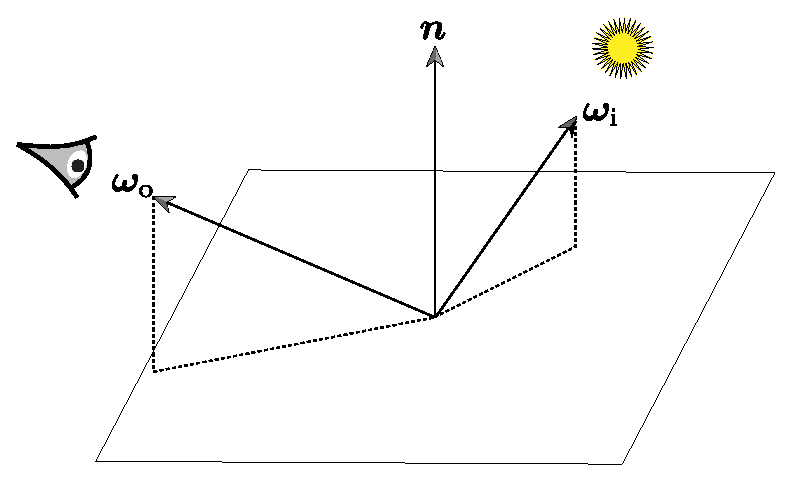
\includegraphics[width=0.5\linewidth]{chap05/BRDF.eps}
    \caption{BRDF。双向反射分布函数是在一对方向${\bm\omega}_{\mathrm{i}}$
        和${\bm\omega}_{\mathrm{o}}$上描述有多少沿${\bm\omega}_{\mathrm{i}}$
        入射的光从表面朝方向${\bm\omega}_{\mathrm{o}}$散射的4D函数。}
    \label{fig:5.18}
\end{figure}

如果方向${\bm\omega}_{\mathrm{i}}$视作方向的微分锥,则$\bm p$处的微分辐照度是
\begin{align}\label{eq:5.7}
    \mathrm{d}E({\bm p},{\bm\omega}_{\mathrm{i}})=L_{\mathrm{i}}({\bm p},{\bm\omega}_{\mathrm{i}})\cos\theta_{\mathrm{i}}\mathrm{d}{\bm\omega}_{\mathrm{i}}\, .
\end{align}

要被反射到方向${\bm\omega}_{\mathrm{o}}$的辐射亮度微分量取决于该辐射照度。
因为几何光学的线性假设,反射的微分辐射亮度正比于辐射照度
\begin{align*}
    \mathrm{d}L_{\mathrm{o}}({\bm p},{\bm\omega}_{\mathrm{o}})\propto\mathrm{d}E({\bm p},{\bm\omega}_{\mathrm{i}})\, .
\end{align*}

比例常数为这对特定方向${\bm\omega}_{\mathrm{i}}$和${\bm\omega}_{\mathrm{o}}$定义了曲面的BRDF:
\begin{align}\label{eq:5.8}
    f_{\mathrm{r}}({\bm p},{\bm \omega}_\mathrm{o},{\bm \omega}_\mathrm{i})=\frac{\mathrm{d}L_{\mathrm{o}}({\bm p},{\bm\omega}_{\mathrm{o}})}{\mathrm{d}E({\bm p},{\bm\omega}_{\mathrm{i}})}=\frac{\mathrm{d}L_{\mathrm{o}}({\bm p},{\bm\omega}_{\mathrm{o}})}{L_{\mathrm{i}}({\bm p},{\bm\omega}_{\mathrm{i}})\cos\theta_{\mathrm{i}}\mathrm{d}{\bm\omega}_{\mathrm{i}}}\, .
\end{align}

基于物理的BRDF有两个重要性质:
\begin{enumerate}
    \item \keyindex{互易性}{reciprocity}{}:对所有方向对${\bm\omega}_{\mathrm{i}}$和${\bm\omega}_{\mathrm{o}}$,
          $f_{\mathrm{r}}({\bm p},{\bm \omega}_\mathrm{i},{\bm \omega}_\mathrm{o})=f_{\mathrm{r}}({\bm p},{\bm \omega}_\mathrm{o},{\bm \omega}_\mathrm{i})$。
    \item {\sffamily 能量守恒}:光反射的总能量少于或等于入射光的能量。
          对于所有方向${\bm\omega}_{\mathrm{o}}$,
          \begin{align*}
              \int\limits_{H^2({\bm n})}f_{\mathrm{r}}({\bm p},{\bm \omega}_\mathrm{o},{\bm \omega}')\cos\theta'\mathrm{d}{\bm\omega}'\le1\, .
          \end{align*}
\end{enumerate}

曲面的\keyindex{双向透射分布函数}{bidirectional transmittance distribution function}{}
(BTDF)描述透射光的分布,可以用和BRDF一样的方法定义。
BTDF一般表示为$f_{\mathrm{t}}({\bm p},{\bm \omega}_\mathrm{o},{\bm \omega}_\mathrm{i})$,
其中${\bm\omega}_{\mathrm{i}}$和${\bm\omega}_{\mathrm{o}}$在绕$\bm p$的相对半球内。
要注意的是,BTDF不遵循上面定义的互异性;
我们将在\refsec{镜面反射与透射}和\refsub{非对称散射}详细讨论该问题。

为了等式的方便,我们把统一考虑时的BRDF和BTDF表示为$f({\bm p},{\bm \omega}_\mathrm{o},{\bm \omega}_\mathrm{i})$;
我们称之为\keyindex{双向散射分布函数}{bidirectional scattering distribution function}{}(BSFD)。
第\refchap{反射模型}将完全专注于描述对渲染有用的各种BSDF。

利用BSDF的定义,我们有
\begin{align*}
    \mathrm{d}L_{\mathrm{o}}({\bm p},{\bm\omega}_{\mathrm{o}})=f({\bm p},{\bm \omega}_\mathrm{o},{\bm \omega}_\mathrm{i})L_{\mathrm{i}}({\bm p},{\bm\omega}_{\mathrm{i}})|\cos\theta_{\mathrm{i}}|\mathrm{d}{\bm\omega}_{\mathrm{i}}\, .
\end{align*}
这里给项$\cos\theta_{\mathrm{i}}$加上了绝对值。
这样做是因为pbrt中曲面法线并没有调整为和${\bm\omega}_{\mathrm{i}}$位于曲面同侧
(许多其他渲染系统都这样做,但我们发现让它们留在原来\refvar{Shape}{}给出的自然朝向会更有用)。
这样做更容易一致地在系统别处运用如“假设曲面法线指向曲面外侧”那样的约定。
因此,像这样给项$\cos\theta_{\mathrm{i}}$加上绝对值保证了实际计算出所需的数量。
我们可以在绕$\bm p$的入射方向球内对该等式积分以计算由于各个方向对$\bm p$的照射
而得到的沿方向${\bm\omega}_{\mathrm{o}}$的出射辐亮度:
\begin{align}\label{eq:5.9}
    L_{\mathrm{o}}({\bm p},{\bm\omega}_{\mathrm{o}})=\int\limits_{S^2}f({\bm p},{\bm \omega}_\mathrm{o},{\bm \omega}_\mathrm{i})L_{\mathrm{i}}({\bm p},{\bm\omega}_{\mathrm{i}})|\cos\theta_{\mathrm{i}}|\mathrm{d}{\bm\omega}_{\mathrm{i}}\, .
\end{align}
这是渲染中的基本方程;它描述了一点的入射光分布
是怎样基于表面的散射性质转化为出射分布的。
当(像这里)球$S^2$作为积分域时它常常称为\keyindex{散射方程}{scattering equation}{},
当只在上半球$H^2({\bm n})$积分时则称\keyindex{反射方程}{reflection equation}{}。
\refchap{光传输I:表面反射}和\refchap{光传输III:双向方法}中积分例程的
关键任务之一就是计算场景中曲面上的点的该积分值。

\subsection{BSSRDF}\label{sub:BSSRDF}


\section{扩展阅读}\label{sec:扩展阅读05}

Meyer是最早严密研究图形学中光谱表示的学者之一
\citep{10.1145/800250.807502}\citep{10.1145/7529.7920}。
\citet{10.1007/978-1-4612-3526-2}总结了1989年光谱表示的最新进展,
\citet{GLASSNER1995}的《\citetitle{GLASSNER1995}》涵盖了20世纪90年代中期的话题。
\citet{773962}、\citet{773963}以及\citet{10.2312:egst.20021054}的研究论文
是关于该话题的优良资源。

\citet{10.1145/122718.122729}分析了三刺激表示用于光谱计算时引入的误差。
\citet{10.1145/166117.166142}以依赖于场景的方法基于选择基函数开发了技术:
通过看向场景中光源和反射物体的SPD,用特征向量分析可以找到
少量能准确表示场景SPD的光谱基函数。
\citet{10.1007/978-3-7091-6858-5_12}将场景中所有SPD投影到层次化基
(\keyindex{哈尔小波}{Haar wavelet}{wavelet小波}
\sidenote{译者注:\keyindex{小波}{wavelet}{}变换指用有限长或快速衰减的“母小波”
    的振荡波形来表示信号。哈尔小波变换是最早提出的最简单小波变换。})上,
并说明了该自适应表示能用来保持在期望的误差界内。
\citet{10.2312:EGWR:EGWR02:117-124}通过在渲染前仔细调整提供给系统的颜色值
为提升来自于只用RGB的常规渲染系统的光谱结果开发了方法。

\citet{Sun2001}研究了另一个光谱表示的方法,
他把SPD分为光滑的基SPD和一组尖峰。
利用与分布每个部分相适配的基函数,每部分的表示都不同。
\citet{Drew:03}应用了一种“尖锐”基,它是自适应的但具有性质即
计算两个基中函数之积不用像许多其他基表示那样进行全矩阵乘法。

当用采样点表示(例如\refvar{SampledSpectrum}{})时,
很难知道对于精确结果需要多少样本。
\citet{Lehtonen:06}研究了这一问题并确定了
5纳米的样本间隔对于真实世界SPD足够了。

\citet{Evans:1999:10.20380/GI1999.07}为表示SPD引入了
分层\sidenote{译者注:原文stratified。}波长聚类:
思想是每次光谱计算都使用在代表性波长上少数固定数目的样本,
它们是依据光源的光谱分布选出的。
后续计算使用不同的波长,这样(基于少量样本的)单独计算会相对高效,
但是在大量次数计算的总和下,可以很好地覆盖波长的整体范围。
与该方法相关的思想是每次计算中只为单个波长算出结果并取全部结果的平均:
这是\citet{10.1145/256157.256158,}和\citet{Morley:2006:}用的方法。

\citet{Radziszewski2009}提出根据单个波长生成光传播路径的技术,
并用高效的SIMD指令在几个额外波长处追踪其贡献。
当模拟粗糙折射边界的色散时用多重重要性采样综合其贡献会得到减小的方差。
\citet{10.1111/cgf.12419}使用波长上的等间隔点样本并展示了
该方法可以怎样用于光子映射和介质渲染。

\citet{31468}写过关于将(例如用户从显示器上选择的)RGB值转化为SPD的欠约束问题的论文。
\citet{10.1080/10867651.1999.10487511}开发了
我们在\refsub{RGB颜色}实现的改进方法。
见\citet{10.1111/cgf.12676}了解该领域最近的工作,
包括精确执行这些转化时对所涉及复杂性的全面讨论。

\citet{9100708}关于辐射度学的书\sidenote{译者注:原文引用1994年第1版,此处引用的是第2版。}是对该话题的精彩介绍。
\citet{PREISENDORFER19653}也以易懂的方式介绍了辐射度学并
深入研究了辐射度学和物理光学的关系。
\citet{Nicodemus1977}仔细定义了BRDF、BSSRDF以及可从中推导出的各种数量。
见\citet{Moon1936}、\citet{Moon1948}以及\citet{10.1002/sapm193918151}了解
对辐射度学的经典早期介绍。
最后,18世纪中叶\citet{Lambert1760}早期关于光度学的开创性著作
已被Dilaura翻译为英文。

正确实现辐射度量学计算会很困难:
遗漏余弦项会算出与所期望的完全不同的结果。
调试这类问题会非常耗时。
\citet{10.1111/j.1467-8659.2010.01722.x}展示了
怎样用C++的类型系统与这些计算中每一项的单位关联,
例如这样使得尝试将辐亮度值加到另一个表示辐照度的值会触发编译时错误。

\section{习题}\label{sec:习题05}
\begin{enumerate}
      \item \circleone 只在单个波长$\lambda=600\text{nm}$上发光的50W灯泡1秒内会射出多少光子?
      \item \circletwo 在pbrt中为光谱基类实现新的表示。
            和本章实现的\refvar{RGBSpectrum}{}与
            \refvar{SampledSpectrum}{}比较的图像质量和渲染时间。
            必须包括荧光灯照明等棘手情况。
      \item \circleone 在单位半径圆盘的法线正上方$h$单位处的一点
            对圆盘有恒定出射辐亮度10W$/$(sr$\cdot$m$^2$),计算该点的辐照度。
            计算两次,一次在立体角上积分,一次在面积上积分。
            (提示:如果一开始结果对不上,可见\refsub{采样单位圆盘}。)
      \item \circleone 类似地,在边长为1的正方形曲面法线正上方1单位的点
            对其出射辐亮度为10W$/$(sr$\cdot$m$^2$),计算该点的辐照度。
\end{enumerate}

\section{译者补充:辐射度学、光度学与色度学}\label{sec:译者补充:辐射度学、光度学与色度学}

\begin{remark}
      本节内容不是原书内容,而是译者根据有关资料\citep{978-7-5640-0658-7,
            wiki:solidangle,GB3102.6-93,enwiki:1052681830,
            wiki:candela,Hoffmann2015,wiki:eye}补充的,请酌情参考和斧正。
\end{remark}

\subsection{辐射度量}\label{sub:辐射度量}
立体角表示一个物体对特定点的三维空间角度,是平面角在三维空间中的类比。
它描述在某一点观测到的物体大小尺度。
例如对于一特定观察点,一个在该点附近的小物体
可能和一个远处的大物体有着相同的立体角。
\begin{definition}
      锥体的\keyindex{立体角}{solid angle}{}大小定义为:
      以锥体的顶点为球心作球面,该锥体在球表面截取的面积与球半径平方之比。
\end{definition}
立体角的单位为\keyindex{球面度}{steradian}{}(sr),是无量纲的导出单位。

\begin{figure}[htbp]
      \centering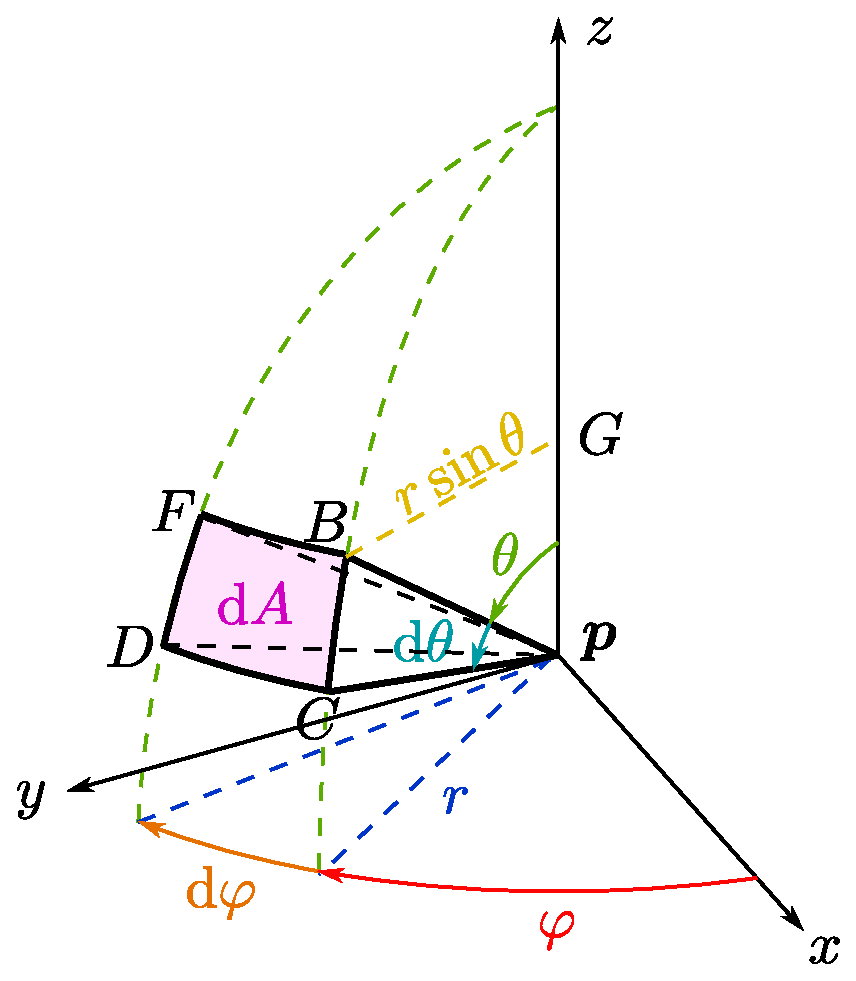
\includegraphics[width=0.4\linewidth]{chap05/ex-solidangle.eps}
      \caption{立体角的定义。}
      \label{fig:5.ex01}
\end{figure}

立体角常用字母$\varOmega$表示。\reffig{5.ex01}展示了一种简单的情形。
以$\bm p$为顶点的微分锥体${\bm p}-BCDF$在同样以$\bm p$为球心且半径为$r$的球面上截取下面元$BCDF$。
建立以$\bm p$为原点的球坐标系,则弧线$\wideparen{BC}$的\keyindex{方位角}{azimuth angle}{}
(在$xy$平面上的投影与原点连线和$x$正半轴所成角)为$\varphi$,
$\wideparen{DF}$方位角为$\varphi+\mathrm{d}\varphi$;
弧线$\wideparen{BF}$的\keyindex{天顶角}{zenith angle}{}(与原点连线和$z$正半轴所成角)为$\theta$,
$\wideparen{CD}$的天顶角为$\theta+\mathrm{d}\theta$。
因此点$B$到其在$z$轴投影点$G$的距离为$r\sin\theta$,
$\wideparen{BF}$的弧长为$r\sin\theta\mathrm{d}\varphi$;
同时$\wideparen{BC}$的弧长为$r\mathrm{d}\theta$。
将面元$BCDF$视作矩形,可求得其微分面积为
\begin{align}
      \mathrm{d}A=r\sin\theta\mathrm{d}\varphi\cdot r\mathrm{d}\theta\, .
\end{align}
依据定义,则相应的立体角元为
\begin{align}
      \mathrm{d}\varOmega=\frac{\mathrm{d}A}{r^2}=\sin\theta\mathrm{d}\theta\mathrm{d}\varphi\, .
\end{align}
对立体角元做曲面积分则可得立体角
\begin{align}
      \varOmega=\iint\limits_S \mathrm{d}\varOmega=\iint\limits_S \sin\theta\mathrm{d}\theta\mathrm{d}\varphi\, .
\end{align}

\begin{corollary}
      封闭曲面对于其内任意一点的立体角均为$4\pi$sr。
\end{corollary}

在连续意义下,我们定义以下辐射度量。

\begin{definition}
      \keyindex{辐射能}{radiant energy}{}指以电磁波形式发射、传播或接收的能量。
\end{definition}
辐射能常用$Q$表示,单位为\keyindex{焦耳}{joule}{}(焦,J)。

\begin{definition}
      \keyindex{辐射能通量}{radiant energy flux}{},
      也称\keyindex{辐射功率}{radiant power}{},
      指电磁辐射通过某一面积发射、传播或接收的功率。
\end{definition}
辐通量常用$\varPhi$表示,单位为\keyindex{瓦特}{watt}{}(瓦,W)。
它描述单位时间内的辐射能:
\begin{align}
      \varPhi=\frac{\mathrm{d}Q}{\mathrm{d}t}\, ,
\end{align}
其中$t$表示时间。

\begin{definition}
      \keyindex{辐射照度}{irradiance}{}/\keyindex{辐射出射度}{radiant exitance}{}指
      照射/离开表面一点处的单位面元上的辐射能通量。
\end{definition}
辐射照度常用$E$表示,辐射出射度常用$M$表示,单位均为$\text{W}/\text{m}^2$。
它们定义中面元所对应的立体角是辐射的整个半球空间,与辐通量的关系为
\begin{align}
      E(\text{或}M)=\frac{\mathrm{d}\varPhi}{\mathrm{d}A}\, ,
\end{align}
其中$A$为表面面积。

\begin{definition}
      \keyindex{辐射强度}{radiant intensity}{}指
      在给定方向的单位立体角元内离开点辐射源(或辐射源面元)的辐射通量。
\end{definition}
辐射强度常用$I$表示,单位为$\text{W}/\text{sr}$。
它一般适合于描述(近似)点光源的辐射方向特性,
与辐射通量和立体角的关系为
\begin{align}
      I=\frac{\mathrm{d}\varPhi}{\mathrm{d}\varOmega}\, .
\end{align}

\begin{definition}
      \keyindex{辐射亮度}{radiance}{}指
      表面一点在垂直于给定方向的单位面元上于该方向的辐射强度。
\end{definition}
辐射亮度常用$L$表示,单位为W$/$(sr$\cdot$m$^2$)。
它与其他辐射度量的关系为
\begin{align}\label{eq:5.ex-radiance}
      L=\frac{\mathrm{d}I}{\cos\theta\mathrm{d}A}=\frac{\mathrm{d}^2\varPhi}{\cos\theta\mathrm{d}A\mathrm{d}\varOmega}=\frac{\mathrm{d}E}{\cos\theta\mathrm{d}\varOmega}\, ,
\end{align}
其中$\theta$是曲面法线与给定方向的夹角。

\reffig{5.ex02}展示了辐射度量之间的微分关系。
\begin{figure}[htbp]
      \centering
      \begin{picture}(370,50)
            \put(0,0){辐射能$Q$}
            \put(45,3){\vector(1,0){40}}
            \put(50,6){时间$t$}
            \put(90,0){辐射通量$\varPhi$}
            \put(150,3){\vector(1,0){50}}
            \put(152,6){立体角$\varOmega$}
            \put(205,0){辐射强度$I$}
            \put(260,3){\vector(1,0){50}}
            \put(262,6){投影面积}
            \put(315,0){辐射亮度$L$}
            \put(120,12){\line(0,1){25}}
            \put(120,37){\vector(1,0){80}}
            \put(152,40){面积$A$}
            \put(205,35){辐射照度$E$}
            \put(260,37){\line(1,0){80}}
            \put(340,37){\vector(0,-1){25}}
            \put(262,40){余弦加权立体角}
      \end{picture}
      \caption{辐射度量的微分关系。}
      \label{fig:5.ex02}
\end{figure}

\subsection{光度学}\label{sub:光度学}
光度量是光辐射能为平均人眼接收所引起的视觉刺激大小的度量。
光度量和辐射度量的定义是一一对应的,都可以用来定量描述辐射的大小。
辐射度量是辐射能本身的客观度量,是纯粹的物理量;
而光度量则还考虑了生理学、心理学等因素。

\keyindex{发光强度}{luminous intensity}{}与辐射强度对应,
单位为坎德拉。
\begin{definition}
      频率为$540\times10^{12}\text{Hz}$(对应空气中555nm的波长)的单色辐射光源
      在给定方向上辐射强度为$\displaystyle\frac{1}{683}$W$/$sr时,
      其发光强度为1\keyindex{坎德拉}{candela}{}(cd)。
\end{definition}
坎德拉是国际单位制七个基本单位之一。
一只普通蜡烛的发光强度约为1cd。

\keyindex{光通量}{luminous flux}{}与辐射通量对应,
单位为\keyindex{流明}{lumen}{}(lm),1lm$=$1cd$\cdot$sr。

\begin{notation}
      我们约定后文光度量和对应的辐射度量所用字母相同,作区分时两者分别添加下标$\mathrm{v}$和$\mathrm{e}$。
      例如辐射强度记为$I_{\mathrm{e}}$,发光强度记为$I_{\mathrm{v}}$。
\end{notation}

\begin{notation}
      某一量的光谱密集度通常表示为波长(或频率)的函数,它具有该量除以波长的量纲,
      有时也称分布函数,为了简便也可用形容词“光谱(的)”代替“光谱密集度”。
      后文中我们约定这类量用下标$\lambda$标记。
      例如“辐射能通量的光谱密集度”可简称为“光谱辐射能通量”,记为$\varPhi_{\lambda}$,
      与辐射能通量$\varPhi$的关系是$\displaystyle\varPhi=\int \varPhi_{\lambda}\mathrm{d}\lambda$。
      但应注意到形容词“光谱(的)”也可用来表示某个量是波长(或频率)的函数,
      这类量的记号把$\lambda$写在圆括号内。
\end{notation}

人感知到的光的强弱与光的频率(波长)有关,这是人眼视觉系统特性决定的。
例如在辐射功率一定时,人眼会感觉黄绿光比红光和蓝光看起来更明亮。
为了描述光源发出可见光的能力,我们引入新的指标。

\begin{definition}
      \keyindex{光视效能}{luminous efficacy}{}是
      目视引起刺激的光通量与光源发出的辐射通量之比,
      记作$K$,单位为lm$/$W:
      \begin{align}
            K=\frac{\varPhi_{\mathrm{v}}}{\varPhi_{\mathrm{e}}}\, .
      \end{align}
\end{definition}

\reftab{5.ex01}列出了常见光源的光视效能。
\begin{table}[htbp]
      \centering
      \begin{tabular}{lc|lc}
            \toprule
            \textbf{光源类型} & \textbf{光视效能(lm$/$W)} & \textbf{光源类型} & \textbf{光视效能(lm$/$W)} \\
            \midrule
            钨丝灯(真空)    & 8.0 - 9.2                 & 日光灯            & 27 - 41                   \\
            钨丝灯(充气)    & 9.2 - 21.0                & 高压水银灯        & 34 - 45                   \\
            石英卤钨灯        & 30                        & 超高压水银灯      & 40.0 - 47.5               \\
            气体放电管        & 16 - 30                   & 钠光灯            & 60                        \\
            \bottomrule
      \end{tabular}
      \caption{常见光源的光视效能。}
      \label{tab:5.ex01}
\end{table}

\begin{definition}
      \keyindex{光谱光视效能}{spectral luminous efficacy}{luminous efficacy光视效能}记作$K(\lambda)$,是光视效能关于波长的函数,即
      \begin{align}
            K(\lambda)=\frac{\varPhi_{\mathrm{v}\lambda}}{\varPhi_{\mathrm{e}\lambda}}\, .
      \end{align}
\end{definition}

\begin{definition}
      $K(\lambda)$的最大值称为\keyindex{最大光谱光视效能}{maximum spectral luminous efficacy}{luminous efficacy光视效能},
      记作$K_{\mathrm{m}}$。它在频率为$540\times10^{12}\text{Hz}$时取得,值为683lm$/$W。
\end{definition}
这也是坎德拉的定义以该频率为标准的原因。

\begin{definition}
      \keyindex{光视效率}{luminous efficiency}{}记作$V$,定义为光视效能与最大光谱光视效能的比值,量纲为1:
      \begin{align}
            V=\frac{K}{K_{\mathrm{m}}}\, .
      \end{align}
\end{definition}

\begin{definition}
      \keyindex{光谱光视效率}{spectral luminous efficiency}{}函数,
      即光视效率关于波长的函数,也称\keyindex{光度函数}{luminosity function}{}、
      相对\keyindex{视见函数}{visual sensitivity function}{}等,记作$V(\lambda)$:
      \begin{align}
            V(\lambda)=\frac{K(\lambda)}{K_{\mathrm{m}}}\, .
      \end{align}
      它表征了人眼对各波长单色光的视觉灵敏度。
\end{definition}

因为人眼在不同亮度环境下的视觉灵敏度不同,所以$V(\lambda)$
分为\keyindex{明视觉}{photopic}{}和\keyindex{暗视觉}{scotopic}{}两种常用版本(\reffig{5.ex03})。
1971年国际照明委员会公布的明视觉的$V(\lambda)$标准值已于1972年由国际计量委员会批准。
\begin{figure}[htbp]
      \centering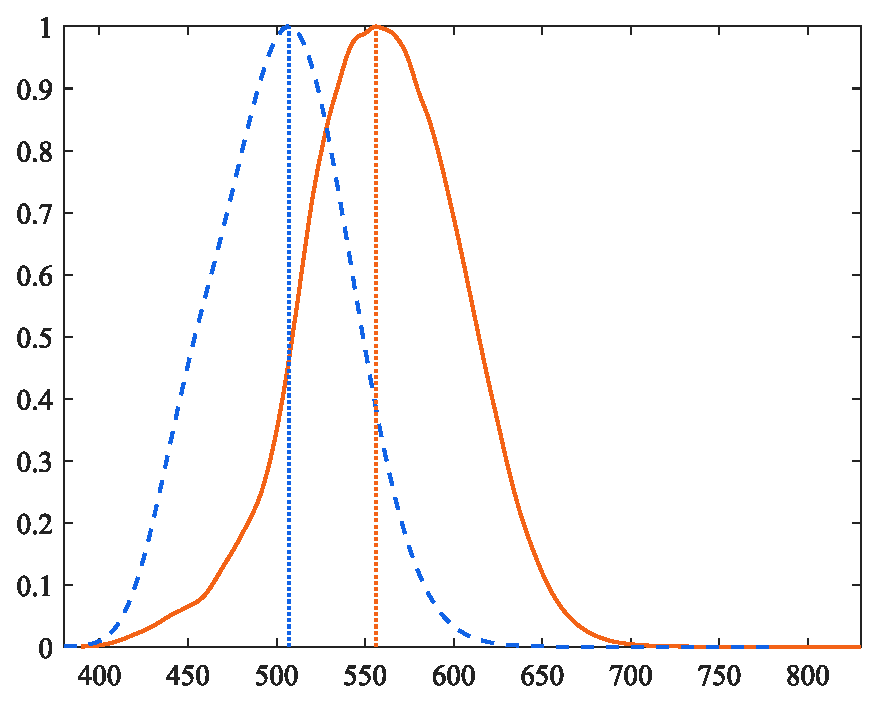
\includegraphics[width=0.75\linewidth]{chap05/spectralluminousefficiency.eps}
      \put(0,0){$\lambda/$nm}
      \put(-315,110){$V(\lambda)$}
      \caption{光谱光视效率曲线。其中橙色实线对应明视觉($2^{\circ}$视场角),蓝色虚线对应暗视觉。
            数据来源于\protect\url{http://www.cvrl.org}。}
      \label{fig:5.ex03}
\end{figure}

依据以上定义,可以推导出如下关系:
\begin{align}
      K                    & =\frac{\displaystyle\int \varPhi_{\mathrm{v}\lambda}\mathrm{d}\lambda}{\displaystyle\int \varPhi_{\mathrm{e}\lambda}\mathrm{d}\lambda}=\frac{\displaystyle\int K(\lambda)\varPhi_{\mathrm{e}\lambda}\mathrm{d}\lambda}{\displaystyle\int \varPhi_{\mathrm{e}\lambda}\mathrm{d}\lambda}\, , \\
      \varPhi_{\mathrm{v}} & =\displaystyle\int K(\lambda)\varPhi_{\mathrm{e}\lambda}\mathrm{d}\lambda=K_{\mathrm{m}}\int V(\lambda)\varPhi_{\mathrm{e}\lambda}\mathrm{d}\lambda\, ,                                                                                                                                    \\
      V                    & =\frac{\displaystyle\int V(\lambda)\varPhi_{\mathrm{e}\lambda}\mathrm{d}\lambda}{\displaystyle\int \varPhi_{\mathrm{e}\lambda}\mathrm{d}\lambda}\, .
\end{align}

\keyindex{光照度}{illuminance}{}与辐射照度对应,
\keyindex{光出射度}{luminous exitance}{}与辐射出射度对应,
单位均为\keyindex{勒克斯}{lux}{}(lx),1lx=1lm$/$m$^2$。

\keyindex{光亮度}{luminance}{}与辐射亮度对应,单位为cd$/$m$^2$。

\subsection{色度学}\label{sub:色度学}
\keyindex{色度学}{colorimetry}{}在物理上量化描述人类颜色知觉的科学技术。
\subsubsection*{人眼视觉特性与颜色视觉理论}
人眼(\reffig{5.ex04})中负责感光的部分是\keyindex{视网膜}{retina}{},
其中具有两种\keyindex{感光细胞}{photoreceptor cell}{},
即\keyindex{视杆细胞}{rod cell}{}和\keyindex{视锥细胞}{cone cell}{}。
视杆细胞主要分布在视网膜中心周围,几乎全部用于夜视力,数量达到一亿量级。
1个光子就足以激发视杆细胞的活动,其对单个光子的敏感程度是视锥细胞的一百多倍,
因此视杆细胞建立人类在夜晚最基本的视觉,即暗视觉。
暗视觉只有视杆细胞起作用,由其仅含的视紫红色素吸收光子,所以不能分辨颜色,只有明暗感觉。
视锥细胞大多分布在视网膜黄斑处,因树突呈锥形得名,约有六百万个。
它主要负责颜色识别,在相对较亮的光照条件下发挥作用(一般需要数十到上百个光子激发),
按所含有的视色素分为三种,分别对黄绿色、绿色和蓝紫色的光最为敏感(\reffig{5.ex05}),
其形成的视觉信号复合后呈现出色彩缤纷的世界。
\begin{figure}[htbp]
      \centering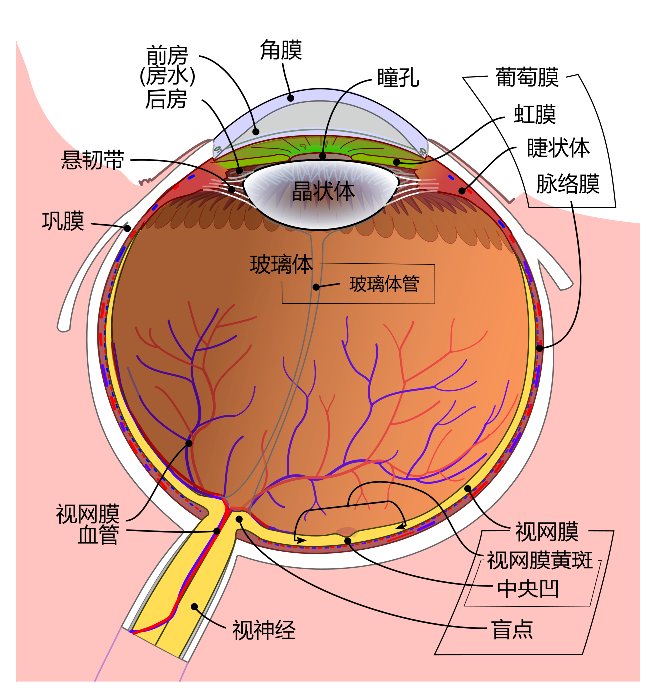
\includegraphics[width=0.5\linewidth]{chap05/Schematic_diagram_of_the_human_eye_zh-hans.eps}
      \caption{人眼结构。}
      \label{fig:5.ex04}
\end{figure}

\begin{figure}[htbp]
      \centering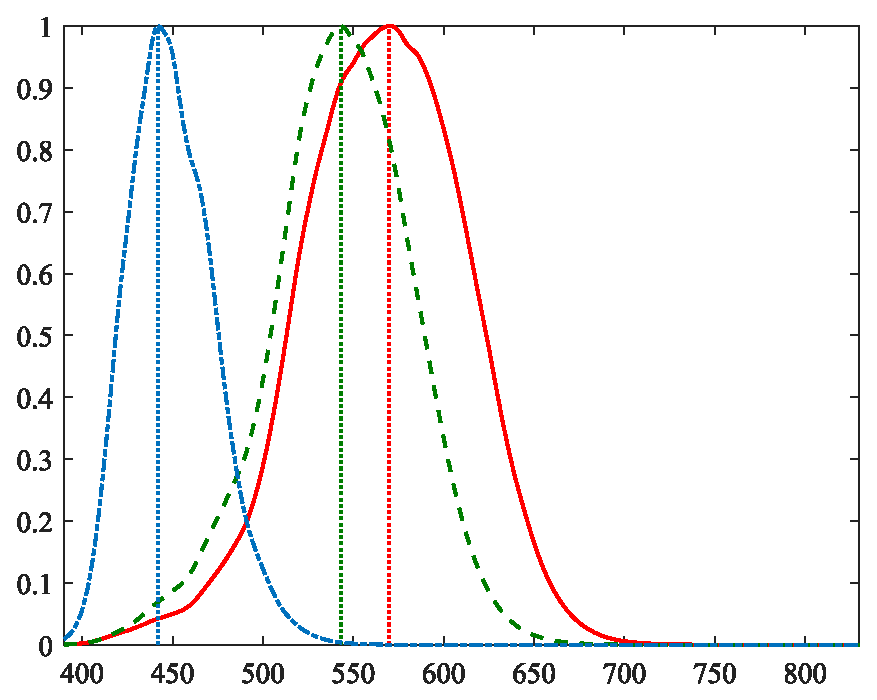
\includegraphics[width=0.75\linewidth]{chap05/NormalizedResponsivitySpectra.eps}
      \put(0,0){$\lambda/$nm}
      \put(-300,35){\rotatebox{90}{规范化视锥响应度(线性能量)}}
      \caption{人眼三种视锥细胞的规范化响应光谱($2^{\circ}$)。
            蓝、绿、红曲线分别对应S、M、L型视锥细胞。
            注意它们的响应绝对峰值并不相同,图中是规范化到0-1后的结果。
            数据来源于\protect\url{http://www.cvrl.org}。}
      \label{fig:5.ex05}
\end{figure}

现代颜色视觉理论主要有两大类,分别从是Yang-Helmholtz的三色学说和Hering的“对立”颜色学说发展起来的。
两者学说都能解释大量事实,但也都有不足之处。
三色学说能很好地说明各种颜色的混合现象,但不能很好地解释色盲现象;“对立”颜色学说则相反。
也有学者试图调和两者的观点。

\subsubsection*{颜色匹配}
\keyindex{颜色混合}{color mixing}{}可以是颜色光的混合,也可以是染料的混合,两种混合方法的结果是不同的,
前者称为\keyindex{加色混合}{additive mixing}{color mixing颜色混合},
后者称为\keyindex{减色混合}{subtractive mixing}{color mixing颜色混合}(\reffig{5.ex06})。
\begin{figure}[htb]
      \centering
      
\includegraphics[width=0.4\linewidth]{chap05/additivemixing.eps}
      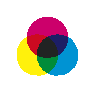
\includegraphics[width=0.4\linewidth]{chap05/subtractivemixing.eps}
      \caption{颜色混合:加色混合(左)与减色混合(右)。}
      \label{fig:5.ex06}
\end{figure}

1853年,德国学者格拉斯曼(Hermann Günther Gra{\ss}mann)利用加色混合
进行了\keyindex{颜色匹配}{color matching}{}实验(\reffig{5.ex07}),
并总结出加色混合的定性性质,即\keyindex{格拉斯曼定律}{Grassmann's laws}{},
为现代色度学的建立奠定了基础。

\begin{proposition}
      格拉斯曼定律的现代解释有四点内容:
      \begin{enumerate}
            \item 人的视觉只能分辨颜色的三种变化(例如明度、色调、饱和度)。
            \item 在由两种成分组成的混合色光中,若一种成分连续变化,则混合色光外观也连续变化。
            \item 存在光谱功率分布不同但外观相同的色光。
            \item 混合色光的总亮度是各成分亮度之和。
      \end{enumerate}
\end{proposition}
\begin{corollary}
      每种色光都存在\keyindex{互补色}{complementary color}{},
      使得两者混合后要么产生无色(白或灰)光,要么产生近似比重大的颜色成分的非饱和色。
\end{corollary}
\begin{corollary}
      任意两种非互补色混合会产生中间色,其色调和饱和度决定于两种成分的色调与相对数量。
\end{corollary}
\begin{corollary}
      若两种色光的外观相同,则它们在加色或减色混合中作成分时的效应是等价的。
\end{corollary}

例如若有两对颜色外观相同,即$A\equiv B$,$C\equiv D$,则有
\begin{align}
      A+C      & \equiv B+D\, ,      \\
      A-C      & \equiv B-D\, ,      \\
      \alpha A & \equiv \alpha B\, ,
\end{align}
其中符号“$\equiv$”表示颜色互相匹配。
即加色、减色混合的外观相同,颜色同时扩大或缩小相同倍数$\alpha>0$的外观相同。
这揭示了颜色混合的线性性质。

\begin{figure}[htbp]
      \centering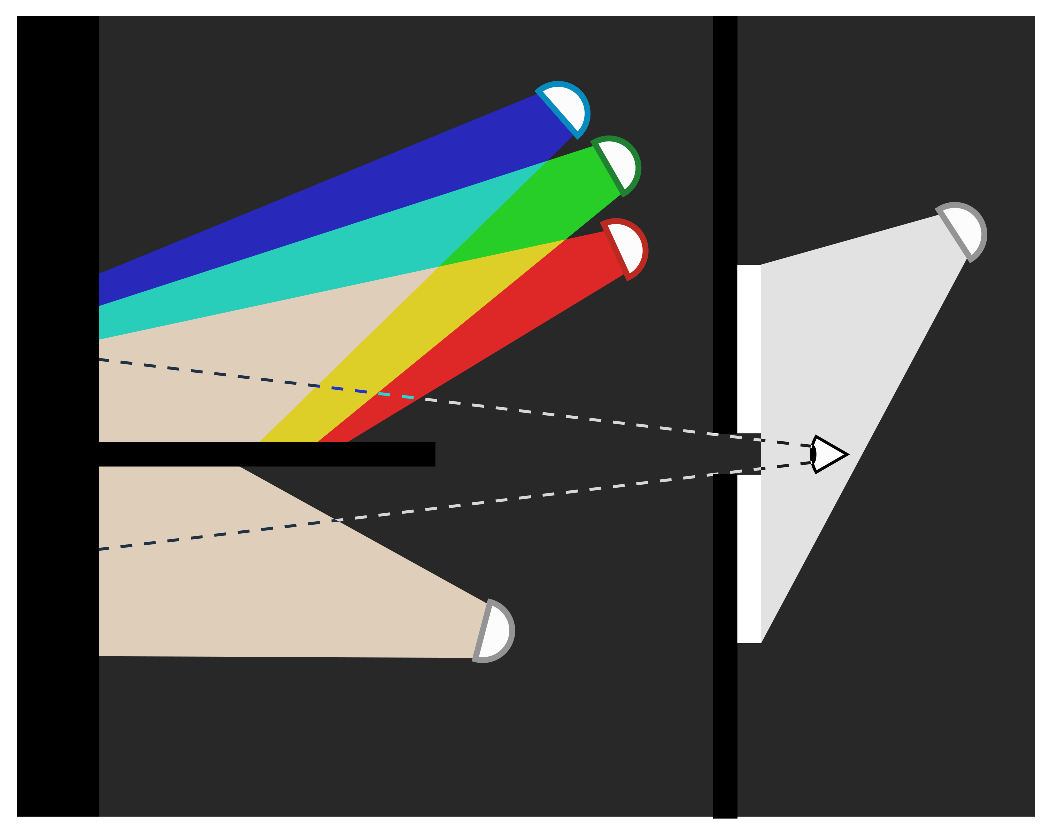
\includegraphics[width=0.75\linewidth]{chap05/colormatching.eps}
      \put(-120,195){\color[RGB]{6,139,190}蓝}
      \put(-105,178){\color[RGB]{31,129,49}绿}
      \put(-105,153){\color[RGB]{187,42,33}红}
      \put(-180,30){\color[RGB]{222,206,186}待匹配颜色光}
      \put(-155,95){\color{white}黑挡片}
      \put(-40,95){\color{white}眼}
      \put(-50,170){\color{white}背景光}
      \caption{颜色匹配实验。}
      \label{fig:5.ex07}
\end{figure}

结合来自1928年莱特(W. David Wright)、1931年吉尔德(John Guild)
以及1931年国际照明委员会(CIE)的颜色匹配实验数据,
CIE提出了“CIE 1931标准色度系统”。它们的实验方法都如\reffig{5.ex07}所示。
左边是一块白色屏幕,上方为红、绿、蓝三原色光,下方为待测色光。
三原色光照射白色屏幕的上半部分,待测色光照射下半部分,中间用黑挡片隔开。
从白色屏幕反射出来的光通过小孔抵达观察者人眼,视场为$2^{\circ}$并被分为两部分。
此外右上方还有一束颜色和强度可调的光照射在小孔周围的背景白板上。
在实验中,调节红、绿、蓝三原色光,直到观察者认为与待测色光的外观相同,
即视场中分界线感觉消失,两部分合为整体,此时即三原混合色光与待测色光达到颜色匹配。
达到匹配后,改变背景光,此时视场中的颜色会变化,但仍能匹配。
颜色匹配时所需三原色的数量称为\keyindex{三刺激值}{tristimulus values}{}。
若分别以$\compcolor{C},\compcolor{R},\compcolor{G},\compcolor{B}$表示
被匹配的颜色以及红、绿、蓝三原色光的单位,以实数$C,R,G,B$表示相应颜色的数量,
则颜色匹配方程可写作
\begin{align}
      C\compcolor{C}\equiv R\compcolor{R}+G\compcolor{G}+B\compcolor{B}\, ,
\end{align}
其中符号“$\equiv$”表示颜色外观相同,$R,G,B$可以为负。

实验还证明了颜色匹配恒常律,即互相匹配的颜色在观察环境变化后依然保持匹配。
实验中在相应规定条件下视场为$2^{\circ}$的观察者
称为\keyindex{CIE 1931标准观察者}{CIE 1931 standard observer}{}。

颜色匹配实验中有个重要问题是:以什么样的颜色作为三原色光?
三刺激值的单位$\compcolor{R},\compcolor{G},\compcolor{B}$如何确定?
原则上,三原色可以任意选定,但其中任何一种颜色不能由其他两种加色混合得到,最常用的是红、绿、蓝。
CIE在实验中使用波长分别为700nm、546.1nm、435.8nm的\keyindex{单色光}{monochromatic light}{}作为三原色,
其中700nm是可见光谱的红色末端,546.1nm和435.8nm是明显的汞谱线,三者在实验中都能比较精确地产生。
为了确定单位,CIE规定能匹配\keyindex{等能白光}{equal-energy white}{}(
也称\keyindex{E光源}{illuminant E}{},即整个光谱功率分布为常数的混合光,
因颜色接近白色得名,是一种理论光源,现实中暂无法模拟出来)且使得三刺激值全等
(即$R=G=B$)的三原色比例作为相应的色度学单位。
实验与测算结果是,红绿蓝按光亮度之比为$1:4.5907:0.0601$
(对应于辐亮度之比$72.0962:1.3791:1$)作为三刺激值的单位。
\begin{example}
      按$0.1\compcolor{R}+0.2\compcolor{G}+0.3\compcolor{B}$所得的色光
      指按$(0.1\times1):(0.2\times4.5907):(0.3\times0.0601)=0.1:0.91814:0.01803$的
      光亮度比例混合波长分别700nm、546.1nm、435.8nm的单色光所得的结果。
\end{example}

实验中还发现,有一些颜色无论如何也无法被三原色匹配出来。
此时将某些三原色挪到与待测色光的同一侧进行实验则能实现匹配。
例如将红光与待测色光放在一侧,绿和蓝色光放在另一侧,当达到匹配时有
\begin{align}
      C\compcolor{C}+R'\compcolor{R}\equiv G\compcolor{G}+B\compcolor{B}\, .
\end{align}
于是可视作
\begin{align}
      C\compcolor{C}\equiv -R'\compcolor{R}+G\compcolor{G}+B\compcolor{B}\, ,
\end{align}
即三刺激值的红色分量为负值$-R'$。

单个波长的可见光称为\keyindex{光谱色}{spectral color}{}。
CIE依据历史与实验测定了匹配等能光谱色的RGB三刺激值,规范化后
得到RGB的\keyindex{颜色匹配函数}{color matching functions}{color matching颜色匹配},
记作$\bar{r}(\lambda),\bar{g}(\lambda),\bar{b}(\lambda)$,
并对应构建了\keyindex{CIE 1931 RGB 颜色空间}{CIE 1931 RGB color space}{}。
\reffig{5.ex08}显示$\bar{r}(\lambda)$在一定波长范围内取负值。
\begin{figure}[htbp]
      \centering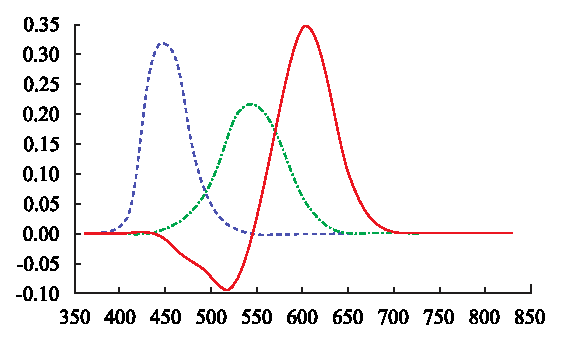
\includegraphics[width=0.75\linewidth]{chap05/CIERGBcolormatchingfunctions.eps}
      \put(10,0){$\lambda/$nm}
      \put(-110,125){$\bar{r}(\lambda)$}
      \put(-170,125){$\bar{g}(\lambda)$}
      \put(-235,125){$\bar{b}(\lambda)$}
      \caption{CIE RGB颜色匹配函数($2^{\circ}$视场),图示来自\citet{SETCHELL2012219}。}
      \label{fig:5.ex08}
\end{figure}

对于光谱分布为$S(\lambda)$的光刺激,相应的RGB值通过在颜色匹配函数上积分算得:
\begin{align}
      R & =k\int \bar{r}(\lambda)S(\lambda)\mathrm{d}\lambda\, , \\
      G & =k\int \bar{g}(\lambda)S(\lambda)\mathrm{d}\lambda\, , \\
      B & =k\int \bar{b}(\lambda)S(\lambda)\mathrm{d}\lambda\, ,
\end{align}
其中$k$为适当的规范化系数。

\subsubsection*{CIE 1931颜色空间}
\begin{definition}
      对于RGB三刺激值为$R,G,B$的颜色,定义其RGB\keyindex{色品}{chromaticity}{}坐标为:
      \begin{align}
            r & =\frac{R}{R+G+B}\, , \\
            g & =\frac{G}{R+G+B}\, , \\
            b & =\frac{B}{R+G+B}\, .
      \end{align}
\end{definition}
\begin{corollary}
      色品坐标之和恒为1,即$r+g+b=1$。
\end{corollary}
这意味着色品坐标中只有两个独立分量。

依据RGB颜色匹配函数$\bar{r}(\lambda),\bar{g}(\lambda),\bar{b}(\lambda)$计算
出光谱色的色品坐标$r,g,b$,并以其中的$r$为横坐标,$g$为纵坐标,
按波长顺序将光谱色的色品点连接起来,可以得到舌形的轨迹(\reffig{5.ex09}),
称为\keyindex{光谱轨迹}{spectral locus}{}。
该轨迹在CIE RGB三原色波长处与坐标轴相交\sidenote{请读者思考一下为什么。},
即在435.8nm处有$r=0,g=0$,在546.1nm处有$r=0,g=1$,在700nm处有$r=1,g=0$。
光谱轨迹及其起点与终点的连线围成封闭区域,
即构成\keyindex{CIE 1931 RGB 颜色空间}{CIE 1931 RGB color space}{}。
注意与\reffig{5.ex08}结合起来思考波长较短的轨迹为何进入$r<0$的半平面。
\begin{figure}[htbp]
      \centering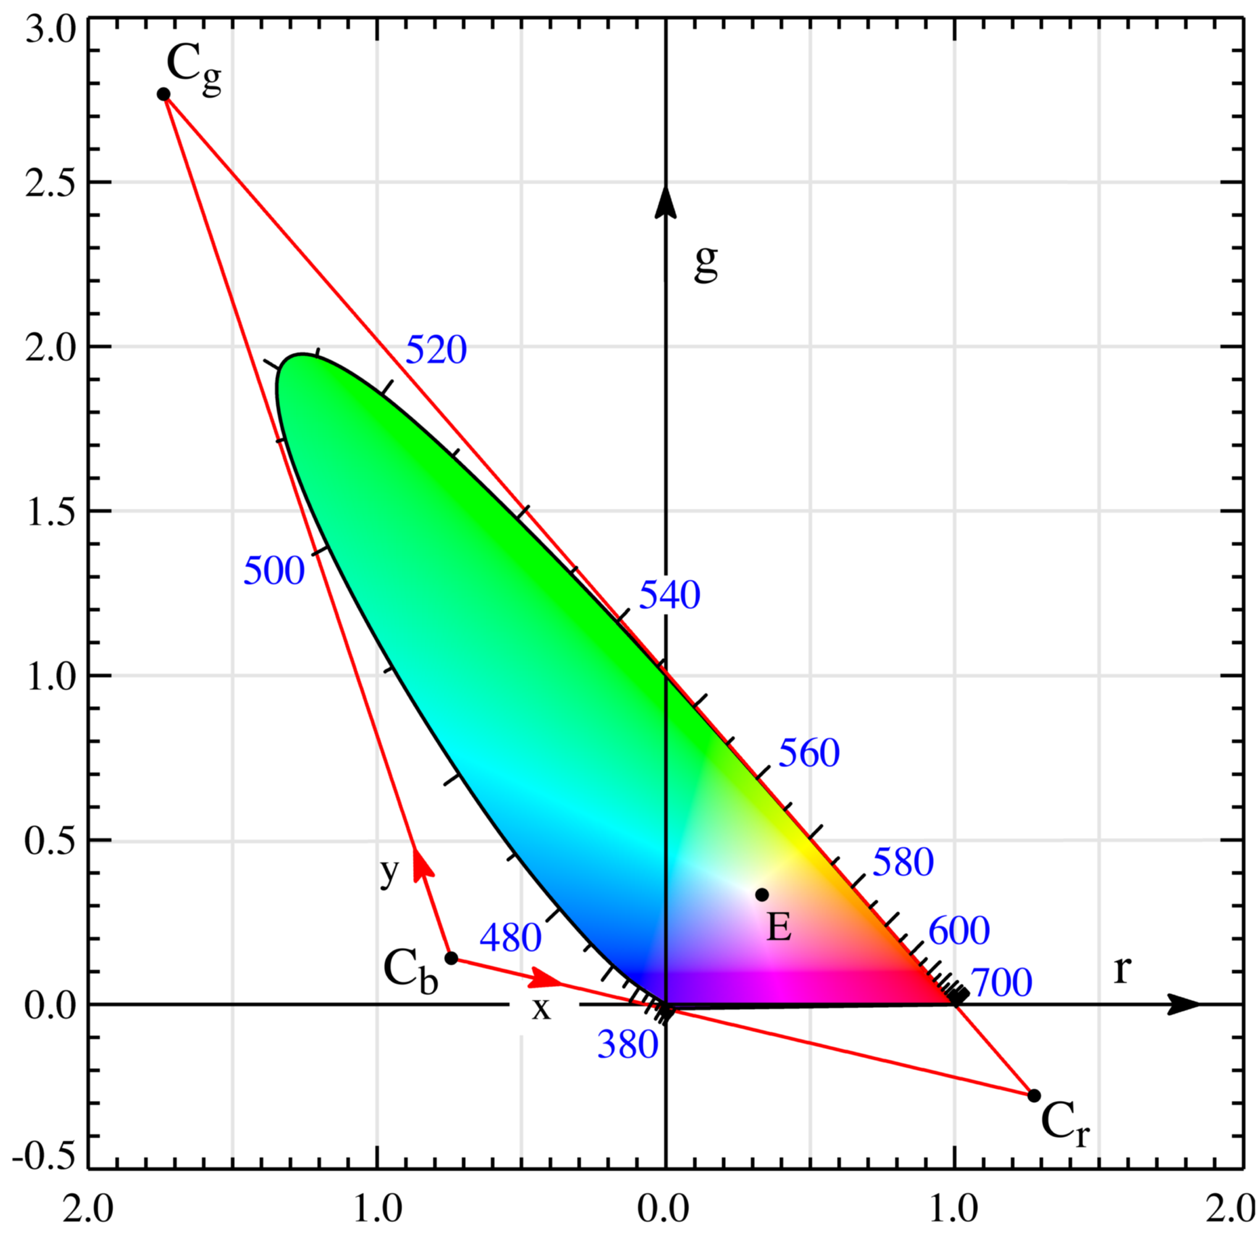
\includegraphics[width=0.75\linewidth]{chap05/CIE1931rgxy.png}
      \caption{CIE $rg$色品空间。其中E为等能白光。}
      \label{fig:5.ex09}
\end{figure}

依据颜色混合的线性性质,我们有:
\begin{corollary}
      对于由任意两种颜色$A,B$加色混合所得的颜色$C$,
      其色品点一定在$A$与$B$色品点所连的线段上。
\end{corollary}



{\noindent\hfil$=========$\hfil{\color{red}{施工分割线}}\hfil$=========$\

\chapterimage{Pictures/chap06/landscape-dof-960x1920.png}
\chapter{相机模型}\label{chap:相机模型}
\setcounter{sidenote}{1}

在第\refchap{绪论}中,我们介绍了计算机图形学中常用的针孔相机模型。
该模型很容易描述和模拟,但它忽略了真实相机中透镜对于穿过的光线具有的重要效应。
例如,针孔相机渲染的所有东西都是清晰对焦的——真实透镜系统不可能达到这种状态。
这样的图像常常看得出来是计算机生成的。
更一般地,离开透镜系统的辐射分布和进入它的分布有很大区别;
对透镜的这种效应建模对于准确模拟成像的辐射度量非常重要。

相机透镜系统也会引入各种影响其所构建图像的\keyindex{像差}{aberration}{};
例如,因为能到达胶片或传感器边缘的光比中心处更少,
\keyindex{暗角}{vignetting}{}\sidenote{译者注:也称晕影。}导致图像边缘变暗。
透镜也可以造成\keyindex{枕状畸变}{pincushion distortion}{distortion畸变}或\keyindex{桶状畸变}{barrel distortion}{distortion畸变},
即让直线成像为曲线。
尽管透镜设计者尽力在其设计中最小化像差,但它们仍可对图像有明显作用。

像第\refchap{形状}的\refvar{Shape}{}那样,pbrt中的相机也表示为抽象基类。
本章介绍类\refvar{Camera}{}及其两个关键方法\refvar[GenerateRay]{Camera::GenerateRay}{()}
和\refvar[GenerateRayDifferential]{Camera::GenerateRayDifferential}{()}。
第一个方法计算对应于胶片平面上样本位置的世界空间光线。
通过基于不同成像模型的不同方法生成这些光线,pbrt中的相机可以创建同一3D场景的多种图像。
第二种方法不仅生成该光线还计算采样该光线的图像区域的信息;
例如该信息用于第\refchap{纹理}的抗锯齿计算。
在\refsub{采样相机2}将介绍一些额外的\refvar{Camera}{}方法以支持双向光传输算法。

本章中,我们将展示\refvar{Camera}{}接口的一些实现,
从实现具有一定普遍性的理想针孔模型开始,
到和真实世界相机一样能模拟光穿过一组玻璃透镜元件成像的逼真模型结束。

\section{相机模型}\label{sec:相机模型}

\label{code:overview_Camera}
\begin{lstlisting}
`\initcode{Camera Declarations}{=}\initnext{CameraDeclarations}`
class Camera {
public:
    `\refcode{Camera Interface}{}`
    `\refcode{Camera Public Data}{}`
};
\end{lstlisting}

\section{投影相机模型}\label{sec:投影相机模型}

三维计算机图形学中的一个基本问题是{\itshape 3D视见问题}:
如何将三维场景投影到二维图像上进行显示。
大多数经典方法都可以用$4\times4$的\keyindex{投影变换}{projective transformation}{transformation变换}矩阵来表达。
因此,我们将引入一个投影矩阵相机类\refvar{ProjectiveCamera}{},
然后在此基础上定义两个相机模型。
第一个实现了\keyindex{正交投影}{orthographic projection}{projection投影},
另一个实现了\keyindex{透视投影}{perspective projection}{projection投影}——
两种经典且广泛使用的\keyindex{投影}{projection}{}。
\begin{lstlisting}
`\initcode{Camera Declarations}{+=}\lastcode{CameraDeclarations}`
class `\initvar{ProjectiveCamera}{}` : public `\refvar{Camera}{}` {
public:
    `\refcode{ProjectiveCamera Public Methods}{}`
protected:
    `\refcode{ProjectiveCamera Protected Data}{}`
};
\end{lstlisting}

还有三个坐标系(总结于\reffig{6.1}中)对定义和讨论投影相机很有用。
\begin{itemize}
    \item \keyindex{屏幕空间}{screen space}{}:
          屏幕空间定义在胶片平面上。相机将相机空间中的物体投影到胶片平面上;
          \keyindex{屏幕窗口}{screen window}{}内的部分在生成的图像中是可见的。
          屏幕空间的深度$z$值从0变到1,分别对应近处和远处截平面的点。
          注意,虽然这称为“屏幕”空间,但它仍然是一个三维坐标系,因为$z$值是有意义的。
    \item \keyindex{规范化设备坐标}{normalized device coordinate}{}(NDC){\sffamily 空间}:
          这是被渲染的实际图像的坐标系。对于$x$和$y$,该空间范围从$(0,0)$变到$(1,1)$,
          其中$(0,0)$是图像的左上角。深度值与屏幕空间中的相同,线性变换将屏幕空间转换为NDC空间。
    \item \keyindex{栅格空间}{raster space}{}\sidenote{译者注:也称光栅空间。}:
          这与NDC空间几乎相同,除了$x$和$y$坐标从$(0,0)$变到(resolution.x, resolution.y)
          \sidenote{译者注:resolution指分辨率。}。
\end{itemize}

投影相机用$4\times4$矩阵在所有这些空间之间进行转换,
但具有特殊成像特性的相机不必用矩阵表示所有这些转换。
\begin{figure}[htbp]
    \centering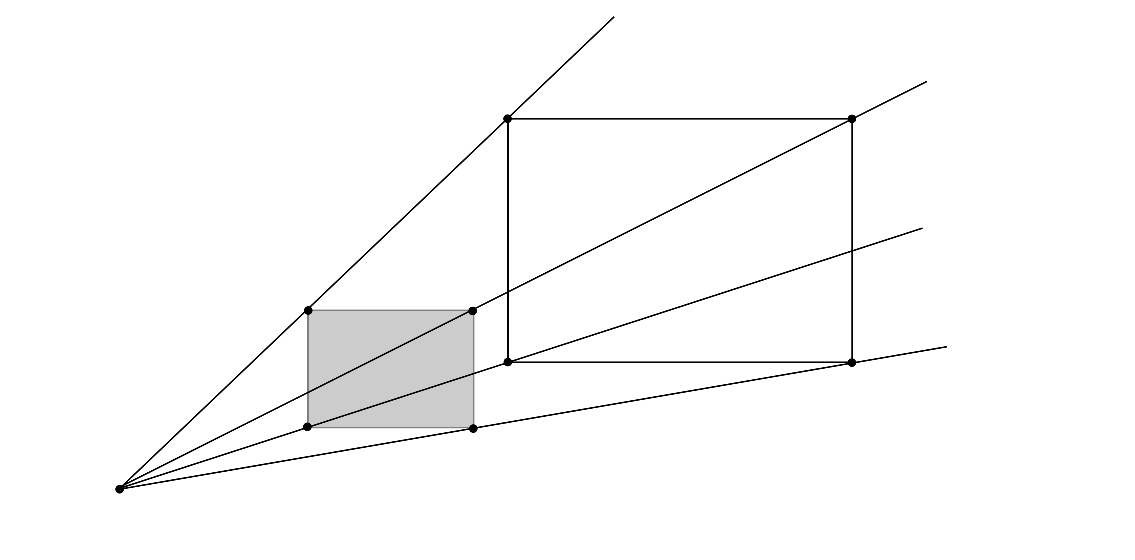
\includegraphics[width=0.75\linewidth]{chap06/Cameracoordinatespaces.eps}
    \put(-280,0){\small 相机空间:$(0,0,0)$}
    \put(-270,60){\small NDC:$(0,0,0)$}
    \put(-220,110){\small NDC:$(0,0,1)$}
    \put(-160,20){\small $z=\text{near}$}
    \put(-160,10){\small NDC:$(1,1,0)$}
    \put(-160,0){\small 栅格:$(\text{res}.x,\text{res}.y,0)$}
    \put(-70,35){\small $z=\text{far}$}
    \put(-70,25){\small NDC:$(1,1,1)$}
    \put(-70,15){\small 栅格:$(\text{res}.x,\text{res}.y,1)$}
    \caption{几个与相机相关的坐标空间常用于简化\protect\refvar{Camera}{}的实现。
        相机类持有它们之间的变换。世界空间中的场景物体由相机查看,它位于相机空间原点,并指向$+z$轴。
        近处和远处平面之间的物体被投影到相机空间中的胶片平面$z=\text{near}$上。
        胶片平面在栅格空间中$z=0$处,其中$x$和$y$范围从$(0,0)$变到(resolution.x, resolution.y)。
        规范化设备坐标(NDC)空间将栅格空间归一化,因此$x$和$y$范围从$(0,0)$变到$(1,1)$。}
    \label{fig:6.1}
\end{figure}

除了基类\refvar{Camera}{}要求的参数外,\refvar{ProjectiveCamera}{}还接收投影变换矩阵、
图像的屏幕空间范围以及与景深有关的额外参数。
\keyindex{景深}{depth of field}{}将在本节末尾介绍和实现,
它模拟了真实透镜系统中出现的失焦物体的模糊性。
\begin{lstlisting}
`\initcode{ProjectiveCamera Public Methods}{=}`
`\refvar{ProjectiveCamera}{}`(const `\refvar{AnimatedTransform}{}` &CameraToWorld, 
        const `\refvar{Transform}{}` &CameraToScreen, const `\refvar{Bounds2f}{}` &screenWindow,
        `\refvar{Float}{}` shutterOpen, `\refvar{Float}{}` shutterClose, `\refvar{Float}{}` lensr, `\refvar{Float}{}` focald,
        `\refvar{Film}{}` *film, const `\refvar{Medium}{}` *medium)
    : `\refvar{Camera}{}`(CameraToWorld, shutterOpen, shutterClose, film, medium),
      `\refvar{CameraToScreen}{}`(CameraToScreen) {
    `\refcode{Initialize depth of field parameters}{}`
    `\refcode{Compute projective camera transformations}{}`
}
\end{lstlisting}

\refvar{ProjectiveCamera}{}的实现将投影变换传递给这里展示的基类构造函数。
该变换给出了相机到屏幕的投影;
由此,构造函数能轻松算出从栅格空间到相机空间一路所需的其他变换。
\begin{lstlisting}
`\initcode{Compute projective camera transformations}{=}`
`\refcode{Compute projective camera screen transformations}{}`
`\refvar{RasterToCamera}{}` = `\refvar[Transform::Inverse]{Inverse}{}`(CameraToScreen) * `\refvar{RasterToScreen}{}`;
\end{lstlisting}
\begin{lstlisting}
`\initcode{ProjectiveCamera Protected Data}{=}\initnext{ProjectiveCameraProtectedData}`
`\refvar{Transform}{}` `\initvar{CameraToScreen}{}`, `\initvar{RasterToCamera}{}`;
\end{lstlisting}

在构造函数中唯一要计算的重要变换是屏幕到栅格的投影。
在下面的代码中,请注意变换的组成(从下往上看),
我们从屏幕空间的一个点开始,先平移使得屏幕左上角位于原点,
然后用屏幕宽度和高度的倒数进行缩放,
得到一个$x$和$y$坐标在0到1之间的点(这些是NDC坐标)。
最后,我们用栅格化分辨率进行缩放,这样我们最终就能完全覆盖
从$(0,0)$直到整个栅格分辨率的栅格范围。
这里一个重要细节是$y$坐标被该变换倒置了;
这是必要的,因为增加的$y$值在屏幕坐标中是向上移动但在栅格坐标中是向下的。
\begin{lstlisting}
`\initcode{Compute projective camera screen transformations}{=}`
`\refvar{ScreenToRaster}{}` = `\refvar{Scale}{}`(film->`\refvar{fullResolution}{}`.x, 
                       film->`\refvar{fullResolution}{}`.y, 1) *
    `\refvar{Scale}{}`(1 / (screenWindow.`\refvar{pMax}{}`.x - screenWindow.`\refvar{pMin}{}`.x),
          1 / (screenWindow.`\refvar{pMin}{}`.y - screenWindow.`\refvar{pMax}{}`.y), 1) *
    `\refvar{Translate}{}`(`\refvar{Vector3f}{}`(-screenWindow.`\refvar{pMin}{}`.x, -screenWindow.`\refvar{pMax}{}`.y, 0));
`\refvar{RasterToScreen}{}` = `\refvar[Transform::Inverse]{Inverse}{}`(`\refvar{ScreenToRaster}{}`);
\end{lstlisting}
\begin{lstlisting}
`\refcode{ProjectiveCamera Protected Data}{+=}\lastnext{ProjectiveCameraProtectedData}`
`\refvar{Transform}{}` `\initvar{ScreenToRaster}{}`, `\initvar{RasterToScreen}{}`;
\end{lstlisting}

\subsection{正交相机}\label{sub:正交相机}
\begin{lstlisting}
`\initcode{OrthographicCamera Declarations}{=}`
class `\initvar{OrthographicCamera}{}` : public `\refvar{ProjectiveCamera}{}` {
public:
    `\refcode{OrthographicCamera Public Methods}{}`
private:
    `\refcode{OrthographicCamera Private Data}{}`
};
\end{lstlisting}

定义在文件\href{https://github.com/mmp/pbrt-v3/blob/master/src/cameras/orthographic.h}{\ttfamily cameras/orthographic.h}和
\href{https://github.com/mmp/pbrt-v3/tree/master/src/cameras/orthographic.cpp}{\ttfamily cameras/orthographic.cpp}中的\keyindex{正交相机}{orthographic camera}{camera相机},
是基于正交投影变换的。
正交变换取场景中的一块矩形区域并将其投影到定义该区域之框的前方一面。
它不具有\keyindex{前缩}{foreshortening}{}效应——当物体远离时它们在成像平面上变小——
但它让平行线依然平行,并保留物体间的相对距离。
\reffig{6.2}{}展示了该立方体是如何定义场景可见区域的。
\begin{figure}[htbp]
    \centering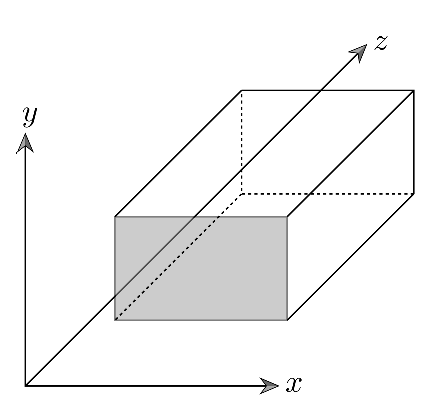
\includegraphics[width=0.33\linewidth]{chap06/Orthoviewingvolume.eps}
    \caption{正交视见体是相机空间中的轴对齐框,
        其定义使该区域内的物体投影到该框$z=\text{near}$的一面上。}
    \label{fig:6.2}
\end{figure}

\reffig{6.3}比较了用正交投影和下节定义的透视投影来渲染的结果
\sidenote{译者注:原图为exr格式,此处转换为png格式以便制作插图,
    图像细节和色域可能发生细微变化。后续均作此处理,读者可到原书官网查看原图。}。
\begin{figure}[htbp]
    \centering
    \subfloat[正交]{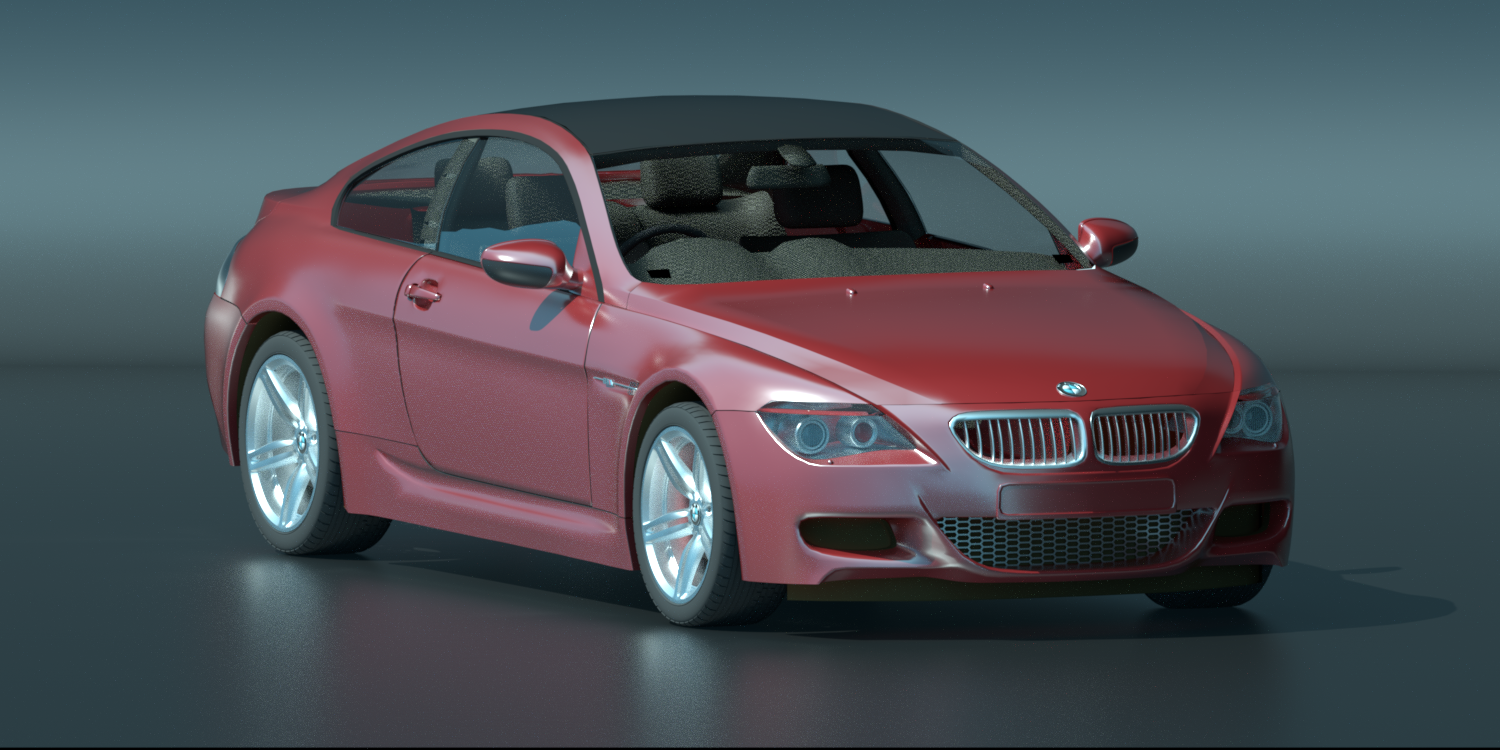
\includegraphics[width=\linewidth]{chap06/car-ortho.png}\label{fig:6.3.1}}\\
    \subfloat[透视]{\includegraphics[width=\linewidth]{chap06/car-perspective.png}\label{fig:6.3.2}}
    \caption{用不同相机模型渲染的汽车模型。用(a)正交和(b)透视相机从同一视点渲染汽车。
        缺少前缩使得正交视角看起来深度更少,但它保留了平行线,是很有用的特性。}
    \label{fig:6.3}
\end{figure}

正交相机构造函数用稍后定义的函数\refvar{Orthographic}{()}生成正交变换矩阵。
\begin{lstlisting}
`\initcode{OrthographicCamera Public Methods}{=}`
`\refvar{OrthographicCamera}{}`(const `\refvar{AnimatedTransform}{}` &CameraToWorld,
        const `\refvar{Bounds2f}{}` &screenWindow, `\refvar{Float}{}` shutterOpen,
        `\refvar{Float}{}` shutterClose, `\refvar{Float}{}` lensRadius, `\refvar{Float}{}` focalDistance,
        `\refvar{Film}{}` *film, const `\refvar{Medium}{}` *medium)
    : `\refvar{ProjectiveCamera}{}`(CameraToWorld, `\refvar{Orthographic}{}`(0, 1),
                       screenWindow, shutterOpen, shutterClose,
                       lensRadius, focalDistance, film, medium) {
    `\refcode{Compute differential changes in origin for orthographic camera rays}{}`
}
\end{lstlisting}

正交视角变换保持$x$和$y$坐标不变但将近处平面的$z$值映射为0而远处平面的$z$值映射为1。
为此,场景先沿$z$轴平移使得近处平面对齐到$z=0$。
然后,场景按$z$缩放使得远处平面映射为$z=1$。
这两个变换合成得到整个变换。(对于像pbrt那样的光线追踪器,
我们想让近处平面位于0处,这样光线就会从穿过相机位置的平面上发出;
远处平面偏移量不是很重要。)
\begin{lstlisting}
`\refcode{Transform Method Definitions}{+=}\lastnext{TransformMethodDefinitions}`
`\refvar{Transform}{}` `\initvar{Orthographic}{}`(`\refvar{Float}{}` zNear, `\refvar{Float}{}` zFar) {
    return `\refvar{Scale}{}`(1, 1, 1 / (zFar - zNear)) *
           `\refvar{Translate}{}`(`\refvar{Vector3f}{}`(0, 0, -zNear));
}
\end{lstlisting}

幸亏正交投影很简单,在方法\refvar[OrthographicCamera::GenerateRayDifferential]{GenerateRayDifferential}{()}中
很容易直接计算$x$和$y$方向的差分射线。
差分射线的方向将和主射线一样(它们对于一个正交相机生成的所有光线都是这样),
且端点差异对于所有射线也会一样。
因此,这里的构造函数预先计算射线端点因胶片平面上在$x$和$y$方向移动单个像素而
在相机空间坐标中移动了多少。
\begin{lstlisting}
`\initcode{Compute differential changes in origin for orthographic camera rays}{=}`
`\refvar[OrthographicCamera::dxCamera]{dxCamera}{}` = `\refvar{RasterToCamera}{}`(`\refvar{Vector3f}{}`(1, 0, 0));
`\refvar[OrthographicCamera::dyCamera]{dyCamera}{}` = `\refvar{RasterToCamera}{}`(`\refvar{Vector3f}{}`(0, 1, 0));
\end{lstlisting}
\begin{lstlisting}
`\initcode{OrthographicCamera Private Data}{=}`
`\refvar{Vector3f}{}` `\initvar[OrthographicCamera::dxCamera]{dxCamera}{}`, `\initvar[OrthographicCamera::dyCamera]{dyCamera}{}`;
\end{lstlisting}

我们现在可以执行代码取栅格空间中的一个样本点并将其变为相机光线。
\reffig{6.4}总结了该过程。首先,栅格空间样本位置变换为相机空间的一点,
即给出近处平面上一点作为相机光线的端点。
因为相机空间观察方向沿$z$轴指出,相机空间光线方向为$(0,0,1)$。

\begin{figure}[htbp]
    \centering\includegraphics[width=0.8\linewidth]{chap06/Orthogenerateray.eps}
    \caption{为了用正交相机创建光线,胶片平面上的栅格空间位置被变换到相机空间,
        给出近处平面上的射线端点。相机空间中光线的方向为$(0,0,1)$,沿$z$轴。}
    \label{fig:6.4}
\end{figure}

若为该场景启用景深,则修改射线端点和方向来模拟景深。本节将稍后解释景深。
光线的时间值通过按偏移量\refvar{CameraSample::time}{}(在范围$[0,1)$内)
在快门开启和关闭间线性插值来设置。最后,光线在被返回前变换到世界空间。
\begin{lstlisting}
`\initcode{OrthographicCamera Definitions}{=}\initnext{OrthographicCameraDefinitions}`
`\refvar{Float}{}` `\refvar{OrthographicCamera}{}`::`\initvar[OrthographicCamera::GenerateRay]{\refvar{GenerateRay}{}}{}`(const `\refvar{CameraSample}{}` &sample,
        `\refvar{Ray}{}` *ray) const {
    `\refcode{Compute raster and camera sample positions}{}`
    *ray = `\refvar{Ray}{}`(pCamera, `\refvar{Vector3f}{}`(0, 0, 1));
    `\refcode{Modify ray for depth of field}{}`
    ray->`\refvar[Ray::time]{time}{}` = `\refvar{Lerp}{}`(sample.`\refvar[CameraSample::time]{time}{}`, `\refvar{shutterOpen}{}`, `\refvar{shutterClose}{}`);
    ray->`\refvar[Ray::medium]{medium}{}` = `\refvar[Camera::medium]{medium}{}`;
    *ray = `\refvar{CameraToWorld}{}`(*ray);
    return 1;
}
\end{lstlisting}

一旦设置好所有变换矩阵,就很容易将栅格空间样本变换到相机空间。
\begin{lstlisting}
`\initcode{Compute raster and camera sample positions}{=}`
`\refvar{Point3f}{}` pFilm = `\refvar{Point3f}{}`(sample.`\refvar{pFilm}{}`.x, sample.`\refvar{pFilm}{}`.y, 0);
`\refvar{Point3f}{}` pCamera = `\refvar{RasterToCamera}{}`(pFilm);
\end{lstlisting}

\refvar[OrthographicCamera::GenerateRayDifferential]{GenerateRayDifferential}{()}的实现执行一样的计算来生成相机主光线。
差分射线端点用在\refvar{OrthographicCamera}{}构造函数中算得的偏移量求出,
然后将整个射线差分变换到世界空间。
\begin{lstlisting}
`\refcode{OrthographicCamera Definitions}{+=}\lastcode{OrthographicCameraDefinitions}`
`\refvar{Float}{}` `\refvar{OrthographicCamera}{}`::`\initvar[OrthographicCamera::GenerateRayDifferential]{\refvar{GenerateRayDifferential}{}}{}`(
        const `\refvar{CameraSample}{}` &sample, `\refvar{RayDifferential}{}` *ray) const {
    `\refcode{Compute main orthographic viewing ray}{}`
    `\refcode{Compute ray differentials for OrthographicCamera}{}`
    ray->`\refvar[Ray::time]{time}{}` = `\refvar{Lerp}{}`(sample.`\refvar[CameraSample::time]{time}{}`, `\refvar{shutterOpen}{}`, `\refvar{shutterClose}{}`);
    ray->`\refvar{hasDifferentials}{}` = true;
    ray->`\refvar[Ray::medium]{medium}{}` = `\refvar[Camera::medium]{medium}{}`;
    *ray = `\refvar{CameraToWorld}{}`(*ray);
    return 1;
}
\end{lstlisting}
\begin{lstlisting}
`\initcode{Compute main orthographic viewing ray}{=}`
`\refcode{Compute raster and camera sample positions}{}`
*ray = `\refvar{RayDifferential}{}`(pCamera, `\refvar{Vector3f}{}`(0, 0, 1));
`\refcode{Modify ray for depth of field}{}`
\end{lstlisting}
\begin{lstlisting}
`\initcode{Compute ray differentials for OrthographicCamera}{=}`
if (`\refvar{lensRadius}{}` > 0) {
    `\refcode{Compute OrthographicCamera ray differentials accounting for lens}{}`
} else {
    ray->`\refvar{rxOrigin}{}` = ray->`\refvar[Ray::o]{o}{}` + `\refvar[OrthographicCamera::dxCamera]{dxCamera}{}`;
    ray->`\refvar{ryOrigin}{}` = ray->`\refvar[Ray::o]{o}{}` + `\refvar[OrthographicCamera::dyCamera]{dyCamera}{}`;
    ray->`\refvar{rxDirection}{}` = ray->`\refvar{ryDirection}{}` = ray->`\refvar[Ray::d]{d}{}`;
}
\end{lstlisting}
\begin{lstlisting}
`\initcode{Compute OrthographicCamera ray differentials accounting for lens}{=}`
`\refcode{Sample point on lens}{}`
`\refvar{Float}{}` ft = focalDistance / ray->`\refvar[Ray::d]{d}{}`.z;

`\refvar{Point3f}{}` pFocus = pCamera + `\refvar[OrthographicCamera::dxCamera]{dxCamera}{}` + (ft * `\refvar{Vector3f}{}`(0, 0, 1));
ray->`\refvar{rxOrigin}{}` = `\refvar{Point3f}{}`(pLens.x, pLens.y, 0);
ray->`\refvar{rxDirection}{}` = `\refvar{Normalize}{}`(pFocus - ray->`\refvar{rxOrigin}{}`);

pFocus = pCamera + `\refvar[OrthographicCamera::dyCamera]{dyCamera}{}` + (ft * `\refvar{Vector3f}{}`(0, 0, 1));
ray->`\refvar{ryOrigin}{}` = `\refvar{Point3f}{}`(pLens.x, pLens.y, 0);
ray->`\refvar{ryDirection}{}` = `\refvar{Normalize}{}`(pFocus - ray->`\refvar{ryOrigin}{}`);
\end{lstlisting}

\subsection{透视相机}\label{sub:透视相机}
透视投影和正交投影相似,也把一个空间体投影到2D胶片平面上。
然而,它包含前缩效应:远处物体比近处相同尺寸的物体投影得更小。
不像正交投影那样,透视投影不保持距离和角度,平行线也不再保持平行。
透视投影非常符合眼睛或相机透镜生成3D世界图像的方式。
投影相机实现于文件\href{https://github.com/mmp/pbrt-v3/blob/master/src/cameras/perspective.h}{\ttfamily cameras/perspective.h}
和\href{https://github.com/mmp/pbrt-v3/blob/master/src/cameras/perspective.cpp}{\ttfamily cameras/perspective.cpp}中。
\begin{lstlisting}
`\initcode{PerspectiveCamera Declarations}{=}`
class `\initvar{PerspectiveCamera}{}` : public `\refvar{ProjectiveCamera}{}` {
public:
    `\refcode{PerspectiveCamera Public Methods}{}`
private:
    `\refcode{PerspectiveCamera Private Data}{}`
};
\end{lstlisting}
\begin{lstlisting}
`\initcode{PerspectiveCamera Method Definitions}{=}\initnext{PerspectiveCameraMethodDefinitions}`
`\refvar{PerspectiveCamera}{}`::`\refvar{PerspectiveCamera}{}`(
        const `\refvar{AnimatedTransform}{}` &CameraToWorld,
        const `\refvar{Bounds2f}{}` &screenWindow, `\refvar{Float}{}` shutterOpen,
        `\refvar{Float}{}` shutterClose, `\refvar{Float}{}` lensRadius, `\refvar{Float}{}` focalDistance,
        `\refvar{Float}{}` fov, `\refvar{Film}{}` *film, const `\refvar{Medium}{}` *medium)
    : `\refvar{ProjectiveCamera}{}`(CameraToWorld, `\refvar{Perspective}{}`(fov, 1e-2f, 1000.f),
                       screenWindow, shutterOpen, shutterClose,
                       lensRadius, focalDistance, film, medium) {
    `\refcode{Compute differential changes in origin for perspective camera rays}{}`
    `\refcode{Compute image plane bounds at z=1 for PerspectiveCamera}{}`
}
\end{lstlisting}

透视投影描述了场景的透视图。
场景中的点投影到垂直于$z$轴的视平面上。
函数\refvar{Perspective}{()}计算该变换;
它接收视场角度{\ttfamily fov}以及到近处$z$平面和远处$z$平面的距离。
在透视投影后,近处$z$平面上的点映射为$z=0$,远处平面上的点则有$z=1$(\reffig{6.5})。
对于基于栅格化的渲染系统,仔细设置这些平面的位置很重要;
它们决定了要渲染的场景的$z$范围,但将它们取值的量级设置得相差过大可能导致数值精度误差。
对于像pbrt的光线追踪器,可以按其位置任意设置它们。
\begin{figure}[htbp]
    \centering\includegraphics[width=0.5\linewidth]{chap06/Perspectivetransformationmatrix.eps}
    \caption{投影变换矩阵将相机空间里的点投影到胶片平面。
        被投影点的$x'$和$y'$坐标等于投影前$x$和$y$坐标除以$z$坐标。
        投影后的$z'$坐标的计算使得近处平面的点映射为$z'=0$而
        远处平面的点映射为$z'=1$。}
    \label{fig:6.5}
\end{figure}

\begin{lstlisting}
`\refcode{Transform Method Definitions}{+=}\lastcode{TransformMethodDefinitions}`
`\refvar{Transform}{}` `\initvar{Perspective}{}`(`\refvar{Float}{}` fov, `\refvar{Float}{}` n, `\refvar{Float}{}` f) {
    `\refcode{Perform projective divide for perspective projection}{}`
    `\refcode{Scale canonical perspective view to specified field of view}{}`
}
\end{lstlisting}
该变换最容易理解,分两个步骤:
\begin{enumerate}
    \item 相机空间的点$\bm p$被投影到视平面上。
          一点代数计算证明视平面上投影后的$x'$和$y'$坐标可计算为$x$和$y$除以点的$z$坐标值。
          投影后的深度$z$被重新映射使近处平面的$z$值为0而远处平面的$z$值为1。
          我们要做的计算为
          \begin{align*}
              x' & =\frac{x}{z}\, ,           \\
              y' & =\frac{y}{z}\, ,           \\
              z' & =\frac{f(z-n)}{z(f-n)}\, .
          \end{align*}
          整个该计算可用齐次坐标编码为$4\times4$矩阵:
          \begin{align*}
              \left[\begin{array}{cccc}
                      1 & 0 & 0             & 0               \\
                      0 & 1 & 0             & 0               \\
                      0 & 0 & \frac{f}{f-n} & -\frac{fn}{f-n} \\
                      0 & 0 & 1             & 0
                  \end{array}\right]
          \end{align*}
          \begin{lstlisting}
`\initcode{Perform projective divide for perspective projection}{=}`
`\refvar{Matrix4x4}{}` persp(1, 0,           0,              0,
                0, 1,           0,              0,
                0, 0, f / (f - n), -f*n / (f - n),
                0, 0,           1,              0);
\end{lstlisting}
    \item 用户指定的视场角({\ttfamily fov})通过缩放投影平面上的$(x,y)$值
          使得视场内的点投影到视平面上坐标$[-1,1]$内来实现。
          对于正方形图像,屏幕空间内$x$和$y$都在$[-1,1]$内。
          否则,图像更窄的那个方向映射到$[-1,1]$,
          更宽的方向映射到成比例的更大屏幕空间值范围。
          回想正切等于直角三角形对边与邻边之比。
          这里邻边长为1,所以对边长为$\tan\frac{\text{\ttfamily fov}}{2}$。
          用该长度倒数缩放将视场映射到$[-1,1]$内的范围。
\end{enumerate}
\begin{lstlisting}
`\initcode{Scale canonical perspective view to specified field of view}{=}`
`\refvar{Float}{}` invTanAng = 1 / std::tan(`\refvar{Radians}{}`(fov) / 2);
return `\refvar{Scale}{}`(invTanAng, invTanAng, 1) * `\refvar{Transform}{}`(persp);
\end{lstlisting}

类似于\refvar{OrthographicCamera}{},关于\refvar{PerspectiveCamera}{}生成的
相机光线如何随着我们移动胶片平面上的像素而改变的信息可在构造函数中预先算出。
这里我们计算相机空间近处投影平面上的位置随像素位置移动而发生的变化。
\begin{lstlisting}
`\initcode{Compute differential changes in origin for perspective camera rays}{=}`
`\refvar[PerspectiveCamera::dxCamera]{dxCamera}{}` = (`\refvar{RasterToCamera}{}`(`\refvar{Point3f}{}`(1, 0, 0)) -
            `\refvar{RasterToCamera}{}`(`\refvar{Point3f}{}`(0, 0, 0)));
`\refvar[PerspectiveCamera::dyCamera]{dyCamera}{}` = (`\refvar{RasterToCamera}{}`(`\refvar{Point3f}{}`(0, 1, 0)) -
            `\refvar{RasterToCamera}{}`(`\refvar{Point3f}{}`(0, 0, 0)));
\end{lstlisting}
\begin{lstlisting}
`\initcode{PerspectiveCamera Private Data}{=}\initnext{PerspectiveCameraPrivateData}`
`\refvar{Vector3f}{}` `\initvar[PerspectiveCamera::dxCamera]{dxCamera}{}`, `\initvar[PerspectiveCamera::dyCamera]{dyCamera}{}`;
\end{lstlisting}

用透视投影时,所有光线都从相机空间原点$(0,0,0)$发出。
光线的方向由从原点指向近处平面上的点{\ttfamily pCamera}的向量给出,
该点对应提供的\refvar{CameraSample}{}的{\ttfamily pFilm}位置。
换句话说,该光线方向向量的每个分量等于该点的位置,
所以不需做无用减法来计算该方向,我们只需直接用点{\ttfamily pCamera}来初始化该方向。
\begin{lstlisting}
`\refcode{PerspectiveCamera Method Definitions}{+=}\lastnext{PerspectiveCameraMethodDefinitions}`
`\refvar{Float}{}` `\refvar{PerspectiveCamera}{}`::`\initvar[PerspectiveCamera::GenerateRay]{\refvar{GenerateRay}{}}{}`(const `\refvar{CameraSample}{}` &sample,
        `\refvar{Ray}{}` *ray) const {
    `\refcode{Compute raster and camera sample positions}{}`
    *ray = `\refvar{Ray}{}`(`\refvar{Point3f}{}`(0, 0, 0), `\refvar{Normalize}{}`(`\refvar{Vector3f}{}`(pCamera)));
    `\refcode{Modify ray for depth of field}{}`
    ray->`\refvar[Ray::time]{time}{}` = `\refvar{Lerp}{}`(sample.`\refvar[CameraSample::time]{time}{}`, `\refvar{shutterOpen}{}`, `\refvar{shutterClose}{}`);
    ray->`\refvar[Ray::medium]{medium}{}` = `\refvar[Camera::medium]{medium}{}`;
    *ray = `\refvar{CameraToWorld}{}`(*ray);
    return 1;
}
\end{lstlisting}

方法\refvar[PerspectiveCamera::GenerateRayDifferential]{GenerateRayDifferential}{()}遵
循\refvar[PerspectiveCamera::GenerateRay]{GenerateRay}{()}的实现,只是多了计算差分射线的代码片。
\begin{lstlisting}
`\initcode{PerspectiveCamera Public Methods}{=}`
`\refvar{Float}{}` `\initvar[PerspectiveCamera::GenerateRayDifferential]{\refvar{GenerateRayDifferential}{}}{}`(const `\refvar{CameraSample}{}` &sample,
                              `\refvar{RayDifferential}{}` *ray) const;
\end{lstlisting}
\begin{lstlisting}
`\initcode{Compute offset rays for PerspectiveCamera ray differentials}{=}`
if (lensRadius > 0) {
    `\refcode{Compute PerspectiveCamera ray differentials accounting for lens}{}`
} else {
    ray->`\refvar{rxOrigin}{}` = ray->`\refvar{ryOrigin}{}` = ray->`\refvar[Ray::o]{o}{}`;
    ray->`\refvar{rxDirection}{}` = `\refvar{Normalize}{}`(`\refvar{Vector3f}{}`(pCamera) + `\refvar[PerspectiveCamera::dxCamera]{dxCamera}{}`);
    ray->`\refvar{ryDirection}{}` = `\refvar{Normalize}{}`(`\refvar{Vector3f}{}`(pCamera) + `\refvar[PerspectiveCamera::dyCamera]{dyCamera}{}`);
}
\end{lstlisting}
\begin{lstlisting}
`\initcode{Compute PerspectiveCamera ray differentials accounting for lens}{=}`
`\refcode{Sample point on lens}{}`
`\refvar{Vector3f}{}` dx = `\refvar{Normalize}{}`(`\refvar{Vector3f}{}`(pCamera + `\refvar[PerspectiveCamera::dxCamera]{dxCamera}{}`));
`\refvar{Float}{}` ft = focalDistance / dx.z;
`\refvar{Point3f}{}` pFocus = `\refvar{Point3f}{}`(0, 0, 0) + (ft * dx);
ray->`\refvar{rxOrigin}{}` = `\refvar{Point3f}{}`(pLens.x, pLens.y, 0);
ray->`\refvar{rxDirection}{}` = `\refvar{Normalize}{}`(pFocus - ray->`\refvar{rxOrigin}{}`);

`\refvar{Vector3f}{}` dy = `\refvar{Normalize}{}`(`\refvar{Vector3f}{}`(pCamera + `\refvar[PerspectiveCamera::dyCamera]{dyCamera}{}`));
ft = focalDistance / dy.z;
pFocus = `\refvar{Point3f}{}`(0, 0, 0) + (ft * dy);
ray->`\refvar{ryOrigin}{}` = `\refvar{Point3f}{}`(pLens.x, pLens.y, 0);
ray->`\refvar{ryDirection}{}` = `\refvar{Normalize}{}`(pFocus - ray->`\refvar{ryOrigin}{}`);
\end{lstlisting}

\subsection{薄透镜模型与景深}\label{sub:薄透镜模型与景深}


\section{环境相机}\label{sec:环境相机}
光线追踪相比扫描线或基于栅格化的渲染方法的一个优点是
它容易利用特殊的图像投影。
在图像样本位置如何映射到光线方向方面我们有很大自由,
因为渲染算法不依赖诸如场景中的直线总是投影为图像中的直线那样的性质。

本节中,我们将介绍绕场景中一点追踪所有方向光线的相机模型,
它给出自该点可见的一切内容的2D视图。
考虑场景中绕相机位置的球;选择该球上的点给定追踪光线的方向。
如果我们用球坐标将该球参数化,则球上的每个点与一对$(\theta,\phi)$关联,
其中$\theta\in[0,\pi]$且$\phi\in[0,2\pi]$
(见\refsub{球坐标上的积分}关于球坐标的更多细节)。
这类图像尤其有用,因为它表示场景中一点的所有入射光
(这类图像表示的一个重要用处是环境照明——场景中使用光的基于图像的表示的渲染技术)。
\reffig{6.14}展示了San Miguel模型中的该相机。
$\theta$值范围从图像顶端的0变到图像底端的$\pi$,
$\phi$值范围由图像左侧到右侧从0变到$2\pi$
\footnote{熟悉制图学的读者会认出这是个\keyindex{等距柱状投影}{equirectangular projection}{projection投影}}。
\begin{lstlisting}
`\initcode{EnvironmentCamera Declarations}{=}`
class `\initvar{EnvironmentCamera}{}` : public `\refvar{Camera}{}` {
public:
    `\refcode{EnvironmentCamera Public Methods}{}`
};
\end{lstlisting}



\section{逼真相机}\label{sec:逼真相机}
\begin{remark}
    本节含有高级内容,第一次阅读时可以跳过。
\end{remark}

薄透镜模型使得能渲染因景深而模糊的图像,
但它只是对多个\keyindex{透镜元件}{lens element}{lens透镜}构成的
真实相机透镜系统非常粗糙的近似,而每个透镜元件都会改变穿过它的辐射分布
(\reffig{6.15}展示了具有8个元件的22mm焦距\keyindex{广角}{wide-angle}{}镜头横截面)。
即使基本的手机相机也趋于有五个左右独立的透镜元件,
而\keyindex{数码单镜头反光相机}{digital single-lens reflex camera}{camera相机}
(数码单反相机,DSLR)镜头可能有十个或更多。
通常,具备更大数量透镜元件的更复杂透镜系统能
比更简单的透镜系统创建更高质量的图像。
\begin{figure}[htbp]
    \centering%LaTeX with PSTricks extensions
%%Creator: Inkscape 1.1.1 (3bf5ae0d25, 2021-09-20)
%%Please note this file requires PSTricks extensions
\psset{xunit=.5pt,yunit=.5pt,runit=.5pt}
\begin{pspicture}(480,210.66666667)
{
\newrgbcolor{curcolor}{0 0 0}
\pscustom[linewidth=1.33333333,linecolor=curcolor]
{
\newpath
\moveto(102.07812533,200.869792)
\curveto(80.78645867,139.869792)(80.78645867,73.46354133)(102.07812533,12.46354133)
}
}
{
\newrgbcolor{curcolor}{0 0 0}
\pscustom[linewidth=1.33333333,linecolor=curcolor]
{
\newpath
\moveto(102.125,200.34895867)
\lineto(129.375,200.34895867)
}
}
{
\newrgbcolor{curcolor}{0 0 0}
\pscustom[linewidth=1.33333333,linecolor=curcolor]
{
\newpath
\moveto(102.125,11.942708)
\lineto(129.375,11.942708)
}
}
{
\newrgbcolor{curcolor}{0 0 0}
\pscustom[linewidth=1.33333333,linecolor=curcolor]
{
\newpath
\moveto(129.375,200.34895867)
\lineto(129.375,177.625)
}
}
{
\newrgbcolor{curcolor}{0 0 0}
\pscustom[linewidth=1.33333333,linecolor=curcolor]
{
\newpath
\moveto(129.375,11.942708)
\lineto(129.375,34.66145867)
}
}
{
\newrgbcolor{curcolor}{0 0 0}
\pscustom[linewidth=1.33333333,linecolor=curcolor]
{
\newpath
\moveto(129.95833333,178.14583333)
\curveto(108.70312533,160.494792)(96.41145867,134.29687467)(96.41145867,106.66666667)
\curveto(96.41145867,79.03645867)(108.70312533,52.83854133)(129.95833333,35.1875)
}
}
{
\newrgbcolor{curcolor}{0 0 0}
\pscustom[linewidth=1.33333333,linecolor=curcolor]
{
\newpath
\moveto(187.03125067,155.77604133)
\curveto(170.58854133,125.09895867)(170.58854133,88.23437467)(187.03125067,57.557292)
}
}
{
\newrgbcolor{curcolor}{0 0 0}
\pscustom[linewidth=1.33333333,linecolor=curcolor]
{
\newpath
\moveto(187.5625,155.255208)
\lineto(211.682292,155.255208)
}
}
{
\newrgbcolor{curcolor}{0 0 0}
\pscustom[linewidth=1.33333333,linecolor=curcolor]
{
\newpath
\moveto(187.5625,57.03125067)
\lineto(211.682292,57.03125067)
}
}
{
\newrgbcolor{curcolor}{0 0 0}
\pscustom[linewidth=1.33333333,linecolor=curcolor]
{
\newpath
\moveto(211.682292,155.255208)
\lineto(211.682292,145.119792)
}
}
{
\newrgbcolor{curcolor}{0 0 0}
\pscustom[linewidth=1.33333333,linecolor=curcolor]
{
\newpath
\moveto(211.682292,57.03125067)
\lineto(211.682292,67.17187467)
}
}
{
\newrgbcolor{curcolor}{0 0 0}
\pscustom[linewidth=1.33333333,linecolor=curcolor]
{
\newpath
\moveto(211.52604133,67.692708)
\curveto(217.22916667,93.364584)(217.22916667,119.96874933)(211.52604133,145.64062533)
}
}
{
\newrgbcolor{curcolor}{0 0 0}
\pscustom[linewidth=1.33333333,linecolor=curcolor]
{
\newpath
\moveto(211.682292,145.119792)
\lineto(231.1875,145.119792)
}
}
{
\newrgbcolor{curcolor}{0 0 0}
\pscustom[linewidth=1.33333333,linecolor=curcolor]
{
\newpath
\moveto(211.682292,67.17187467)
\lineto(231.1875,67.17187467)
}
}
{
\newrgbcolor{curcolor}{0 0 0}
\pscustom[linewidth=1.33333333,linecolor=curcolor]
{
\newpath
\moveto(231.1875,145.119792)
\lineto(231.1875,142.5)
}
}
{
\newrgbcolor{curcolor}{0 0 0}
\pscustom[linewidth=1.33333333,linecolor=curcolor]
{
\newpath
\moveto(231.1875,67.17187467)
\lineto(231.1875,69.79166667)
}
}
{
\newrgbcolor{curcolor}{0 0 0}
\pscustom[linewidth=1.33333333,linecolor=curcolor]
{
\newpath
\moveto(231.33333333,143.02083333)
\curveto(229.77083333,118.807292)(229.77083333,94.52604133)(231.33333333,70.3125)
}
}
{
\newrgbcolor{curcolor}{0 0 0}
\pscustom[linewidth=2.66666667,linecolor=curcolor]
{
\newpath
\moveto(236.510416,140.92708267)
\lineto(236.510416,175.70312533)
}
}
{
\newrgbcolor{curcolor}{0 0 0}
\pscustom[linewidth=2.66666667,linecolor=curcolor]
{
\newpath
\moveto(236.510416,71.364584)
\lineto(236.510416,36.58333333)
}
}
{
\newrgbcolor{curcolor}{0 0 0}
\pscustom[linewidth=1.33333333,linecolor=curcolor]
{
\newpath
\moveto(247.53125067,74.15625067)
\curveto(257.25,94.739584)(257.25,118.59374933)(247.53125067,139.17708267)
}
}
{
\newrgbcolor{curcolor}{0 0 0}
\pscustom[linewidth=1.33333333,linecolor=curcolor]
{
\newpath
\moveto(247.32291733,142.5)
\lineto(266.23437467,142.5)
}
}
{
\newrgbcolor{curcolor}{0 0 0}
\pscustom[linewidth=1.33333333,linecolor=curcolor]
{
\newpath
\moveto(247.32291733,69.79166667)
\lineto(266.23437467,69.79166667)
}
}
{
\newrgbcolor{curcolor}{0 0 0}
\pscustom[linewidth=1.33333333,linecolor=curcolor]
{
\newpath
\moveto(247.32291733,142.5)
\lineto(247.32291733,138.65104133)
}
}
{
\newrgbcolor{curcolor}{0 0 0}
\pscustom[linewidth=1.33333333,linecolor=curcolor]
{
\newpath
\moveto(247.32291733,69.79166667)
\lineto(247.32291733,73.635416)
}
}
{
\newrgbcolor{curcolor}{0 0 0}
\pscustom[linewidth=1.33333333,linecolor=curcolor]
{
\newpath
\moveto(265.98437467,70.3125)
\curveto(276.25,93.46354133)(276.25,119.869792)(265.98437467,143.02083333)
}
}
{
\newrgbcolor{curcolor}{0 0 0}
\pscustom[linewidth=1.33333333,linecolor=curcolor]
{
\newpath
\moveto(273.57812533,64.369792)
\curveto(274.47916667,92.5625)(274.47916667,120.77083333)(273.57812533,148.96354133)
}
}
{
\newrgbcolor{curcolor}{0 0 0}
\pscustom[linewidth=1.33333333,linecolor=curcolor]
{
\newpath
\moveto(274.17187467,151.58854133)
\lineto(278.78125067,151.58854133)
}
}
{
\newrgbcolor{curcolor}{0 0 0}
\pscustom[linewidth=1.33333333,linecolor=curcolor]
{
\newpath
\moveto(274.17187467,60.70312533)
\lineto(278.78125067,60.70312533)
}
}
{
\newrgbcolor{curcolor}{0 0 0}
\pscustom[linewidth=1.33333333,linecolor=curcolor]
{
\newpath
\moveto(274.17187467,151.58854133)
\lineto(274.17187467,148.442708)
}
}
{
\newrgbcolor{curcolor}{0 0 0}
\pscustom[linewidth=1.33333333,linecolor=curcolor]
{
\newpath
\moveto(274.17187467,60.70312533)
\lineto(274.17187467,63.84895867)
}
}
{
\newrgbcolor{curcolor}{0 0 0}
\pscustom[linewidth=1.33333333,linecolor=curcolor]
{
\newpath
\moveto(278.3125,61.22395867)
\curveto(291.4375,72.67708267)(298.97395867,89.244792)(298.97395867,106.66666667)
\curveto(298.97395867,124.08854133)(291.4375,140.65625067)(278.3125,152.10937467)
}
}
{
\newrgbcolor{curcolor}{0 0 0}
\pscustom[linewidth=1.33333333,linecolor=curcolor]
{
\newpath
\moveto(278.78125067,154.90625067)
\lineto(300.739584,154.90625067)
}
}
{
\newrgbcolor{curcolor}{0 0 0}
\pscustom[linewidth=1.33333333,linecolor=curcolor]
{
\newpath
\moveto(278.78125067,57.385416)
\lineto(300.739584,57.385416)
}
}
{
\newrgbcolor{curcolor}{0 0 0}
\pscustom[linewidth=1.33333333,linecolor=curcolor]
{
\newpath
\moveto(278.78125067,154.90625067)
\lineto(278.78125067,151.58854133)
}
}
{
\newrgbcolor{curcolor}{0 0 0}
\pscustom[linewidth=1.33333333,linecolor=curcolor]
{
\newpath
\moveto(278.78125067,57.385416)
\lineto(278.78125067,60.70312533)
}
}
{
\newrgbcolor{curcolor}{0 0 0}
\pscustom[linewidth=1.33333333,linecolor=curcolor]
{
\newpath
\moveto(301.28125067,57.90625067)
\curveto(313.60937467,89.244792)(313.60937467,124.08854133)(301.28125067,155.42708267)
}
}
{
\newrgbcolor{curcolor}{0 0 0}
\pscustom[linewidth=1.33333333,linecolor=curcolor]
{
\newpath
\moveto(310.05208267,53.35937467)
\curveto(329.29166667,64.20833333)(341.192708,84.57812533)(341.192708,106.66666667)
\curveto(341.192708,128.755208)(329.29166667,149.125)(310.05208267,159.97395867)
}
}
{
\newrgbcolor{curcolor}{0 0 0}
\pscustom[linewidth=1.33333333,linecolor=curcolor]
{
\newpath
\moveto(310.46354133,177.625)
\lineto(318.90104133,177.625)
}
}
{
\newrgbcolor{curcolor}{0 0 0}
\pscustom[linewidth=1.33333333,linecolor=curcolor]
{
\newpath
\moveto(310.46354133,34.66145867)
\lineto(318.90104133,34.66145867)
}
}
{
\newrgbcolor{curcolor}{0 0 0}
\pscustom[linewidth=1.33333333,linecolor=curcolor]
{
\newpath
\moveto(310.46354133,177.625)
\lineto(310.46354133,159.45312533)
}
}
{
\newrgbcolor{curcolor}{0 0 0}
\pscustom[linewidth=1.33333333,linecolor=curcolor]
{
\newpath
\moveto(310.46354133,34.66145867)
\lineto(310.46354133,52.83854133)
}
}
{
\newrgbcolor{curcolor}{0 0 0}
\pscustom[linewidth=1.33333333,linecolor=curcolor]
{
\newpath
\moveto(318.75,35.1875)
\curveto(339.32291733,53.244792)(351.114584,79.29166667)(351.114584,106.66666667)
\curveto(351.114584,134.04166667)(339.32291733,160.08854133)(318.75,178.14583333)
}
}
{
\newrgbcolor{curcolor}{0 0 0}
\pscustom[linewidth=1.33333333,linecolor=curcolor]
{
\newpath
\moveto(469.09374933,10.8125)
\lineto(469.09374933,201.47395867)
}
}
{
\newrgbcolor{curcolor}{0 0 0}
\pscustom[linewidth=1.33333333,linecolor=curcolor]
{
\newpath
\moveto(469.09374933,106.14583333)
\lineto(9.57291733,106.14583333)
}
}
\end{pspicture}

    \caption{广角透镜系统的横截面(在pbrt发行版的{\ttfamily scenes/lenses/wide.22mm.dat}
    中)。透镜坐标系统让胶片平面垂直于$z$轴且位于$z=0$处。
    透镜在左边负z轴上,然后场景在透镜左侧。透镜系统中部表示为粗黑线的光圈阻挡命中它的光线。
    在许多透镜系统中,可以调整光圈大小以在更短曝光时间(大光圈)和更大景深(小光圈)间权衡。}
    \label{fig:6.15}
\end{figure}

本节讨论\refvar{RealisticCamera}{}的实现,
它模拟光穿过像\reffig{6.15}那样的透镜系统后聚焦并渲染像\reffig{6.16}那样的图像。
其实现基于光线追踪,即相机追随光路穿过透镜元件,
并考虑具有不同折射率的介质(空气,各类玻璃)间界面的折射,
直到光路要么射出光学系统要么被光圈或镜头罩吸收。
离开前端镜头元件的光线代表相机响应曲线,可用于估计
沿任意光线入射辐亮度的积分器,例如\refvar{SamplerIntegrator}{}。
\refvar{RealisticCamera}{}的实现在文件\href{https://github.com/mmp/pbrt-v3/tree/master/src/cameras/realistic.h}{\ttfamily cameras/realistic.h}
和\href{https://github.com/mmp/pbrt-v3/tree/master/src/cameras/realistic.cpp}{\ttfamily cameras/realistic.cpp}中。
\begin{figure}[htbp]
    \centering\includegraphics[width=0.6\linewidth]{chap06/sanmiguel-fisheye.png}
    \caption{用鱼眼透镜和很宽视场渲染的图像。注意边缘暗处是
        准确模拟成像辐射度量(\refsub{相机测量方程})所致,
        而直线扭曲为曲线则是许多广角镜头的特点,但在用投影矩阵表示透镜投影模型时没有考虑。}
    \label{fig:6.16}
\end{figure}
\begin{lstlisting}
`\initcode{RealisticCamera Declarations}{=}`
class `\initvar{RealisticCamera}{}` : public `\refvar{Camera}{}` {
public:
    `\refcode{RealisticCamera Public Methods}{}`
private:
    `\refcode{RealisticCamera Private Declarations}{}`
    `\refcode{RealisticCamera Private Data}{}`
    `\refcode{RealisticCamera Private Methods}{}`
};
\end{lstlisting}

除了把相机放置于场景中的常见变换、\refvar{Film}{}以及快门打开和关闭的时间外,
\refvar{RealisticCamera}{}构造函数还接收透镜系统描述文件的文件名、
到期望的焦平面的距离以及光圈直径。之后有了第\refchap{蒙特卡罗积分}蒙特卡罗积分与
\refsub{相机测量方程}成像辐射度量的预备知识后,
将在\refsub{采样相机1}介绍参数{\ttfamily simpleWeighting}的作用。
\begin{lstlisting}
`\initcode{RealisticCamera Method Definitions}{=}\initnext{RealisticCameraMethodDefinitions}`
`\refvar{RealisticCamera}{}`::`\refvar{RealisticCamera}{}`(const `\refvar{AnimatedTransform}{}` &CameraToWorld,
        `\refvar{Float}{}` shutterOpen, `\refvar{Float}{}` shutterClose, `\refvar{Float}{}` apertureDiameter,
        `\refvar{Float}{}` focusDistance, bool simpleWeighting, const char *lensFile,
        `\refvar{Film}{}` *film, const `\refvar{Medium}{}` *medium)
    : `\refvar{Camera}{}`(CameraToWorld, shutterOpen, shutterClose, film, medium),
      simpleWeighting(simpleWeighting) {
    `\refcode{Load element data from lens description file}{}`
    `\refcode{Compute lens-film distance for given focus distance}{}`
    `\refcode{Compute exit pupil bounds at sampled points on the film}{}`
}
\end{lstlisting}
\begin{lstlisting}
`\initcode{Load element data from lens description file}{=}`
std::vector<`\refvar{Float}{}`> lensData;
if (ReadFloatFile(lensFile, &lensData) == false) {
    `\refvar{Error}{}`("Error reading lens specification file \"%s\".", lensFile);
    return;
}
if ((lensData.size() % 4) != 0) {
    `\refvar{Error}{}`("Excess values in lens specification file \"%s\"; "
          "must be multiple-of-four values, read %d.",
          lensFile, (int)lensData.size());
    return;
}
for (int i = 0; i < (int)lensData.size(); i += 4) {
    if (lensData[i] == 0) {
        if (apertureDiameter > lensData[i+3]) {
            `\refvar{Warning}{}`("Specified aperture diameter %f is greater than maximum "
                    "possible %f.  Clamping it.", apertureDiameter, lensData[i+3]);
        } else {
            lensData[i+3] = apertureDiameter;
        }
    }
    `\refvar{elementInterfaces}{}`.push_back((`\refvar{LensElementInterface}{}`)
        {lensData[i] * (`\refvar{Float}{}`).001, lensData[i+1] * (`\refvar{Float}{}`).001, lensData[i+2],
         lensData[i+3] * `\refvar{Float}{}`(.001) / `\refvar{Float}{}`(2.)});
}
\end{lstlisting}
\begin{lstlisting}
`\initcode{RealisticCamera Private Data}{=}\initnext{RealisticCameraPrivateData}`
const bool `\initvar{simpleWeighting}{}`;
\end{lstlisting}

在从磁盘加载透镜描述文件之后,构造函数调整透镜与
胶片间的距离使得焦平面位于期望的深度即{\ttfamily focusDistance},
然后预先计算一些关于离胶片最近透镜元件的哪部分面积让光从场景射到胶片的信息,
就像在胶片平面上各点看到的那样。在介绍完背景材料之后,
\refsub{对焦}和\refsub{出射瞳}将分别定义代码片
\refcode{Compute lens-film distance for given focus distance}{}
和\refcode{Compute exit pupil bounds at sampled points on the film}{}。

\subsection{透镜系统表示}\label{sub:透镜系统表示}
透镜系统由一系列透镜元件组成,每个元件通常是某种形制的玻璃。
透镜系统设计者的挑战是在有限空间、成本和生产难度下
设计一组能在胶片或传感器上高质量成像的元件
(例如为了让保持手机变薄,其相机厚度非常有限)。

最容易生产的是横截面为球形的透镜,
透镜系统通常是绕\keyindex{光轴}{optical axis}{}对称的,习惯记为$z$。
我们将假设这两个性质在本节下文中成立。
用胶片对齐到平面$z=0$且透镜在胶片左侧沿$-z$轴放置的坐标系统定义透镜系统。

透镜系统常表示为独立透镜元件(或空气)间的一系列界面,
而不是每个元件的显式表示。\reftab{6.1}展示了定义每个界面的量。
表中最后一项定义了最右边的界面,如\reffig{6.17}所示:
它是个半径等于曲率半径的球体块。元件的厚度是沿$z$到右边下一个
元件(或胶片平面)的距离,\keyindex{折射率}{index of refraction}{}是
对界面右边的介质而言的。元件在$z$轴上下的范围由光圈直径设置。
\begin{table}[htbp]
    \centering
    \begin{tabular}{SSSS}
        \toprule
        \ \ \ \ \textbf{曲率半径} & \ \ \ \ \textbf{厚度} & \ \ \textbf{折射率} & \textbf{光圈直径} \\
        \midrule
        35.98738                  & 1.21638               & 1.54                & 23.716            \\
        11.69718                  & 9.9957                & 1                   & 17.996            \\
        13.08714                  & 5.12622               & 1.772               & 12.364            \\
        -22.63294                 & 1.76924               & 1.617               & 9.812             \\
        71.05802                  & 0.8184                & 1                   & 9.152             \\
        0                         & 2.27766               & 0                   & 8.756             \\
        -9.58584                  & 2.43254               & 1.617               & 8.184             \\
        -11.28864                 & 0.11506               & 1                   & 9.152             \\
        -166.7765                 & 3.09606               & 1.713               & 10.648            \\
        -7.5911                   & 1.32682               & 1.805               & 11.44             \\
        -16.7662                  & 3.98068               & 1                   & 12.276            \\
        -7.70286                  & 1.21638               & 1.617               & 13.42             \\
        -11.97328                 & (取决于焦点)        & 1                   & 17.996            \\
        \bottomrule
    \end{tabular}
    \caption{\reffig{6.15}中透镜系统的表格化描述。每行描述了两个透镜元件间的界面、
        元件与空气间的界面或者光圈。第一行描述了最左边的界面。半径为0的元件对应光圈。
        距离单位为mm。}
    \label{tab:6.1}
\end{table}
\begin{figure}[htbp]
    \centering\includegraphics[width=0.6\linewidth]{chap06/Lenselement.eps}
    \caption{透镜界面(实曲线)与光轴相交于位置$z$。界面几何形状由
        表示其在光轴上下方范围的光圈半径以及元件的曲率半径$r$描述。
        如果元件有球形横截面,则它的轮廓由球心在光轴上距离$r$的球体给定,
        该球体也穿过$z$。如果$r$是负的,则元件界面就如从场景中看到那样是凹的
        (如图所示);否则就是\protect\keyindex{凸}{convex}{}的。透镜厚度给出了到
        右边下一个界面的距离,或者对于最右边的界面是到胶片平面的距离。}
    \label{fig:6.17}
\end{figure}

结构体\refvar{LensElementInterface}{}表示单个透镜元件界面。
\begin{lstlisting}
`\initcode{RealisticCamera Private Declarations}{=}`
struct `\initvar{LensElementInterface}{}` {
    `\refvar{Float}{}` `\initvar{curvatureRadius}{}`;
    `\refvar{Float}{}` `\initvar{thickness}{}`;
    `\refvar{Float}{}` `\initvar[LensElementInterface::eta]{eta}{}`;
    `\refvar{Float}{}` `\initvar{apertureRadius}{}`;
};
\end{lstlisting}

这里没有介绍的代码片\refcode{Load element data from lens description file}{}
\sidenote{译者注:我补充回来了。}读取透镜元件
并初始化数组\refvar[elementInterfaces]{RealisticCamera::elementInterfaces}{}。
见源代码中的注释了解该文件格式的细节,它并行化\reftab{6.1}中的结构,
并见pbrt发行版中的目录{\ttfamily scenes/lenses}了解大量透镜描述示例。

对从文件读取的值做了两个调整:第一,透镜系统传统上用毫米单位描述,
但pbrt假设场景单位用米。因此,除了折射率外的域都按1/1000缩小。
第二,元件直径被除以二;在下面的代码中半径是用起来更方便的量。
\begin{lstlisting}
`\refcode{RealisticCamera Private Data}{+=}\lastnext{RealisticCameraPrivateData}`
std::vector<`\refvar{LensElementInterface}{}`> `\initvar{elementInterfaces}{}`;
\end{lstlisting}

加载完透镜界面描述后,让一些关于透镜系统的值随时可得是很有用的。
\refvar{LensRearZ}{()}和\refvar{LensFrontZ}{()}分别返回
透镜系统尾部和头部元件的$z$深度\sidenote{译者注:靠近胶片的是尾部,远离胶片的是头部。}。
注意返回的$z$深度在相机空间中,而不是透镜空间中,所以为正值。
\begin{lstlisting}
`\initcode{RealisticCamera Private Methods}{=}\initnext{RealisticCameraPrivateMethods}`
`\refvar{Float}{}` `\initvar{LensRearZ}{}`() const {
    return `\refvar{elementInterfaces}{}`.back().`\refvar{thickness}{}`;
}
\end{lstlisting}

求头部元件$z$位置需要求所有元件厚度之和(见\reffig{6.18})。
任何位于系统性能敏感部分的代码都不需要该值,
所以在需要时重算它就行。如果该方法对性能有影响,
最好还是在\refvar{RealisticCamera}{}中缓存该值。
\begin{figure}[htbp]
    \centering\includegraphics[width=0.4\linewidth]{chap06/Elementthicknessandposition.eps}
    \caption{元件厚度与光轴上位置的关系。胶片平面位于$z=0$,尾部元件的厚度$t_3$给出
        了从胶片到其界面的距离;这里尾部界面与轴交于$z=-t_3$。下一个元件厚度为$t_2$且
        位于$z=-t_3-t_2$,以此类推。头部元件交$z$轴于$\sum_i-t_i$。}
    \label{fig:6.18}
\end{figure}
\begin{lstlisting}
`\refcode{RealisticCamera Private Methods}{+=}\lastnext{RealisticCameraPrivateMethods}`
`\refvar{Float}{}` `\initvar{LensFrontZ}{}`() const {
    `\refvar{Float}{}` zSum = 0;
    for (const `\refvar{LensElementInterface}{}` &element : `\refvar{elementInterfaces}{}`)
        zSum += element.`\refvar{thickness}{}`;
    return zSum;
}
\end{lstlisting}

\refvar{RearElementRadius}{()}按单位米返回尾部元件光圈半径。
\begin{lstlisting}
`\refcode{RealisticCamera Private Methods}{+=}\lastnext{RealisticCameraPrivateMethods}`
`\refvar{Float}{}` `\initvar{RearElementRadius}{}`() const {
    return `\refvar{elementInterfaces}{}`.back().`\refvar{apertureRadius}{}`;
}
\end{lstlisting}
\subsection{追踪穿过透镜的光线}\label{sub:追踪穿过透镜的光线}
给定起始于透镜系统胶片一侧的光线,\refvar{TraceLensesFromFilm}{()}依次
计算与每个元件的相交处,如果其路径在穿过透镜系统途中被挡住了就终结该光线并返回{\ttfamily false}。
否则它就返回{\ttfamily true}并用相机空间中退出的光线来初始化{\ttfamily *rOut}。
在遍历时,{\ttfamily elementZ}追踪当前透镜元件的$z$截距。
因为光线起始于胶片,所以按照和\refvar{elementInterfaces}{}存储的相反顺序遍历透镜。
\begin{lstlisting}
`\refcode{RealisticCamera Method Definitions}{+=}\lastnext{RealisticCameraMethodDefinitions}`
bool `\refvar{RealisticCamera}{}`::`\initvar{TraceLensesFromFilm}{}`(const `\refvar{Ray}{}` &rCamera,
        `\refvar{Ray}{}` *rOut) const {
    `\refvar{Float}{}` elementZ = 0;
    `\refcode{Transform rCamera from camera to lens system space}{}`
    for (int i = `\refvar{elementInterfaces}{}`.size() - 1; i >= 0; --i) {
        const `\refvar{LensElementInterface}{}` &element = `\refvar{elementInterfaces}{}`[i];
        `\refcode{Update ray from film accounting for interaction with element}{}`
    }
    `\refcode{Transform rLens from lens system space back to camera space}{}`
    return true;
}
\end{lstlisting}

因为在pbrt的相机空间中相机指向$+z$轴但透镜在$-z$轴,
所以射线端点和方向的$z$分量需要取反。
尽管这是个简单到可以直接施加的变换,
我们还是偏好用显式的\refvar{Transform}{}使目的更明确。
\begin{lstlisting}
`\initcode{Transform rCamera from camera to lens system space}{=}`
static const `\refvar{Transform}{}` CameraToLens = `\refvar{Scale}{}`(1, 1, -1);
`\refvar{Ray}{}` rLens = CameraToLens(rCamera);
\end{lstlisting}

回想\reffig{6.18}中怎样计算元件的$z$截距:
因为我们从后往前访问元件,所以在考虑该元件的作用前
必须从{\ttfamily elementZ}中减去元件的厚度来计算其$z$截距。
\begin{lstlisting}
`\initcode{Update ray from film accounting for interaction with element}{=}`
elementZ -= element.`\refvar{thickness}{}`;
`\refcode{Compute intersection of ray with lens element}{}`
`\refcode{Test intersection point against element aperture}{}`
`\refcode{Update ray path for element interface interaction}{}`
\end{lstlisting}

有了元件的$z$轴截距,下一步是计算沿光线与元件界面(或光圈平面)相交处的参数值$t$。
对于光圈,采用光线-平面测试(见\refsub{光线-边界相交})。
对于球形界面,\refvar{IntersectSphericalElement}{()}执行该测试
并且如果找到相交处则还返回曲面法线;计算折射光方向时将需要该法线。
\begin{lstlisting}
`\initcode{Compute intersection of ray with lens element}{=}`
`\refvar{Float}{}` t;
`\refvar{Normal3f}{}` n;
bool isStop = (element.`\refvar{curvatureRadius}{}` == 0);
if (isStop)
    t = (elementZ - rLens.`\refvar[Ray::o]{o}{}`.z) / rLens.`\refvar[Ray::d]{d}{}`.z;
else {
    `\refvar{Float}{}` radius = element.`\refvar{curvatureRadius}{}`;
    `\refvar{Float}{}` zCenter = elementZ + element.`\refvar{curvatureRadius}{}`;
    if (!`\refvar{IntersectSphericalElement}{}`(radius, zCenter, rLens, &t, &n))
        return false;
}
\end{lstlisting}

方法\refvar{IntersectSphericalElement}{()}大致
和\refvar{Sphere::Intersect}{()}一样,不过它专门针对
元件中心在$z$轴上(且因此中心的$x$和$y$分量为零)这一情况。
这里文中没有包含代码片\refcode{Compute t0 and t1 for ray-element intersection}{}
和\refcode{Compute surface normal of element at ray intersection point}{},因为它们和
\refvar{Sphere::Intersect}{()}的实现一样\sidenote{译者注:我补充回来了。}。
\begin{lstlisting}
`\refcode{RealisticCamera Method Definitions}{+=}\lastnext{RealisticCameraMethodDefinitions}`
bool `\refvar{RealisticCamera}{}`::`\initvar{IntersectSphericalElement}{}`(`\refvar{Float}{}` radius,
        `\refvar{Float}{}` zCenter, const `\refvar{Ray}{}` &ray, `\refvar{Float}{}` *t, `\refvar{Normal3f}{}` *n) {
    `\refcode{Compute t0 and t1 for ray-element intersection}{}`
    `\refcode{Select intersection  based on ray direction and element curvature}{}`
    `\refcode{Compute surface normal of element at ray intersection point}{}`
    return true;
}
\end{lstlisting}
\begin{lstlisting}
`\initcode{Compute t0 and t1 for ray-element intersection}{=}`
`\refvar{Point3f}{}` o = ray.`\refvar[Ray::o]{o}{}` - `\refvar{Vector3f}{}`(0, 0, zCenter);
`\refvar{Float}{}` A = ray.`\refvar[Ray::d]{d}{}`.x*ray.`\refvar[Ray::d]{d}{}`.x + ray.`\refvar[Ray::d]{d}{}`.y*ray.`\refvar[Ray::d]{d}{}`.y + ray.`\refvar[Ray::d]{d}{}`.z*ray.`\refvar[Ray::d]{d}{}`.z;
`\refvar{Float}{}` B = 2 * (ray.`\refvar[Ray::d]{d}{}`.x*o.x + ray.`\refvar[Ray::d]{d}{}`.y*o.y + ray.`\refvar[Ray::d]{d}{}`.z*o.z);
`\refvar{Float}{}` C = o.x*o.x + o.y*o.y + o.z*o.z - radius*radius;
`\refvar{Float}{}` t0, t1;
if (!`\refvar{Quadratic}{}`(A, B, C, &t0, &t1))
    return false;
\end{lstlisting}
\begin{lstlisting}
`\initcode{Compute surface normal of element at ray intersection point}{=}`
*n = `\refvar{Normal3f}{}`(`\refvar{Vector3f}{}`(o + *t * ray.`\refvar[Ray::d]{d}{}`));
*n = `\refvar{Faceforward}{}`(`\refvar{Normalize}{}`(*n), -ray.`\refvar[Ray::d]{d}{}`);
\end{lstlisting}

然而这里在选择返回哪个交点时有个微妙之处\sidenote{译者注:原文subtlety。}:
$t>0$的最近相交处不一定在元件界面上;
见\reffig{6.19}\footnote{“微妙之处”(subtlety)一般意味着作者花费好几个小时来调试它。}。
例如,对于自场景中接近并与(具有负曲率半径的)凹透镜相交的光线,
两个相交处中不管近处那个是否有$t>0$都该返回远处那个。
幸运的是,基于光线方向和曲率半径的简单逻辑可指明用哪个$t$值。
\begin{figure}[htbp]
    \centering\includegraphics[width=0.5\linewidth]{chap06/Lenscorrectintersection.eps}
    \caption{当计算光线与球形透镜元件的相交处时,光线与整球的首个相交处不一定是我们想要的。
        这里,第二个相交处才在真正的元件界面(粗线)上,而第一个应该被忽略。}
    \label{fig:6.19}
\end{figure}
\begin{lstlisting}
`\initcode{Select intersection  based on ray direction and element curvature}{=}`
bool useCloserT = (ray.`\refvar[Ray::d]{d}{}`.z > 0) ^ (radius < 0);
*t = useCloserT ? std::min(t0, t1) : std::max(t0, t1);
if (*t < 0)
    return false;
\end{lstlisting}

每个透镜元件都按某半径绕光轴扩展;如果与该元件的交点在该半径之外,
则该光线实际上将与镜头罩相交并终止。
类似地,如果光线与光圈相交,它也会终止。
因此,这里我们用当前元件的适用限制来测试交点,
要么终止该光线,要么它幸存下来并将其端点更新为当前交点。
\begin{lstlisting}
`\initcode{Test intersection point against element aperture}{=}`
`\refvar{Point3f}{}` pHit = rLens(t);
`\refvar{Float}{}` r2 = pHit.x * pHit.x + pHit.y * pHit.y;
if (r2 > element.`\refvar{apertureRadius}{}` * element.`\refvar{apertureRadius}{}`)
    return false;
rLens.`\refvar[Ray::o]{o}{}` = pHit;
\end{lstlisting}

如果当前元件是光圈,则光路在穿过元件界面时不受影响。
对于玻璃(或塑料)透镜元件,光线在从具有某个折射率的介质进入
到具有另一折射率的介质时在交界面会改变方向
(光线可能从空气进入玻璃、从玻璃进入空气,或者从
具有某个折射率的玻璃进入具有不同折射率的另一种玻璃)。

\refsec{镜面反射与透射}讨论了两种介质边界间折射率的变化
将怎样改变光线的方向及其携带的辐射量(这里的情况下
我们可以忽略辐射量的变化,因为如果光线在进入和退出透镜系统时
处于同一种介质中则这种效应会抵消掉——这里都是空气)。
函数\refvar{Refract}{()}定义在\refsub{镜面透射};
注意它预设入射方向指向远离曲面的方向,所以传入前要对光线方向取反。
该函数在出现\keyindex{全内反射}{total internal reflection}{reflection反射}时
返回{\ttfamily false},该情况下光路终止。
否则在{\ttfamily w}中返回折射方向。

通常,穿过这类界面时一些光被透射而另一些被反射。
这里我们忽略反射并假设完美传输。尽管这是种近似,但它是合理的:
制造透镜时一般用了设计的涂料把反射降低到光线所带辐射的0.25\%左右
(然而,对这少量的反射建模对于实现\keyindex{镜头光晕}{lens flare}{}会很重要)。
\begin{lstlisting}
`\initcode{Update ray path for element interface interaction}{=}`
if (!isStop) {
    `\refvar{Vector3f}{}` w;
    `\refvar{Float}{}` etaI = element.`\refvar[LensElementInterface::eta]{eta}{}`;
    `\refvar{Float}{}` etaT = (i > 0 && `\refvar{elementInterfaces}{}`[i - 1].`\refvar[LensElementInterface::eta]{eta}{}` != 0) ?
        `\refvar{elementInterfaces}{}`[i - 1].`\refvar[LensElementInterface::eta]{eta}{}` : 1;
    if (!`\refvar{Refract}{}`(`\refvar{Normalize}{}`(-rLens.`\refvar[Ray::d]{d}{}`), n, etaI / etaT, &w))
        return false;
    rLens.`\refvar[Ray::d]{d}{}` = w;
}
\end{lstlisting}

若光线成功从前端透镜元件射出,它只需要从透镜空间变换到相机空间。
\begin{lstlisting}
`\initcode{Transform rLens from lens system space back to camera space}{=}`
if (rOut != nullptr) {
    static const `\refvar{Transform}{}` LensToCamera = `\refvar{Scale}{}`(1, 1, -1);
    *rOut = LensToCamera(rLens);
}
\end{lstlisting}

方法\refvar{TraceLensesFromScene}{()}和\refvar{TraceLensesFromFilm}{()}非常相似,这里不再介绍。
主要差别在于它是从前往后而不是从后往前遍历元件。
注意它假设传入的光线已经在相机空间了;
如果光线始于世界空间则调用者应负责执行该变换。
返回的光线位于尾部透镜元件朝向胶片的相机空间中。
\begin{lstlisting}
`\refcode{RealisticCamera Private Methods}{+=}\lastcode{RealisticCameraPrivateMethods}`
bool `\initvar{TraceLensesFromScene}{}`(const `\refvar{Ray}{}` &rCamera, `\refvar{Ray}{}` *rOut) const;
\end{lstlisting}

\subsection{厚透镜近似}\label{sub:厚透镜近似}
\refsub{薄透镜模型与景深}中用的薄透镜近似是基于透镜系统沿光轴厚度为0的简化假设。
透镜系统的厚透镜近似因为考虑了透镜系统的$z$范围而更精确些。
这里在介绍厚透镜的基本概念之后,我们将用厚透镜近似来确定
要把透镜系统放在离胶片多远处来对焦\refsub{对焦}中想要的对焦深度。

厚透镜近似将透镜系统表示为两对沿光轴的距离——
\keyindex{焦点}{focal point}{}以及\keyindex{主平面}{principal plane}{};
一个透镜系统有两个\keyindex{主点}{cardinal point}{}。
如果经由一个理想透镜系统追踪平行于光轴的光线,
则所有这些光线将会交于光轴上同一点——这就是焦点
(实际中,真实透镜系统并不绝对理想,不同高度的入射光线
与光轴将相交于一个$z$值小范围——这就是\keyindex{球面像差}{spherical aberration}{aberration像差})。
有了特定的透镜系统,我们就能从每一侧追踪穿过它且与光轴平行的光线,
并计算它们与$z$轴的相交处以找到焦点(见\reffig{6.20})。
\begin{figure}[htbp]
    \centering\includegraphics[width=\linewidth]{chap06/Lenssystemcardinalpoints.eps}
    \caption{计算透镜系统的主点。文件{\ttfamily lenses/dgauss.dat}中
    描述的透镜系统,来自场景的入射光线平行于光轴(轴上方),
    来自胶片的光线平行于光轴(下方)。这些入射光线对应的
    离开透镜系统的光线与光轴的相交处给出了两个焦点$f'_z$(胶片一侧)
    和$f_z$(场景一侧)。每对入射和出射光线的延长线以及原始光线的相交处给定了
    主平面$z=p_z$和$z=p'_z$,这里表示为垂直于光轴的蓝线。}
    \label{fig:6.20}
\end{figure}

每个主平面通过延长平行于光轴的入射光线以及离开透镜的光线直至相交来求得;
相交处的$z$深度给出了对应主平面的深度。\reffig{6.20}展示了
一个透镜系统及其焦点$f_z$和$f'_z$以及位于$z$值$p_z$和$p'_z$的主平面
(正如\refsub{薄透镜模型与景深},有撇的变量表示透镜系统胶片一侧的点,
无撇的变量表示场景中要成像的点)。

给定离开透镜的光线,求焦点要先计算光线的$x$和$y$分量为零时的值$t_{\mathrm{f}}$。
若进入的光线只沿$x$偏移了光轴,则我们要求出
使$o_x+t_{\mathrm{f}}d_x=0$的$t_{\mathrm{f}}$。因此
\begin{align*}
    t_{\mathrm{f}}=\frac{-o_x}{d_x}\, .
\end{align*}
同样的方法,为了求得离开透镜的光线与原始光线有相同高度处
的主平面的$t_{\mathrm{p}}$,我们有$o_x+t_{\mathrm{p}}d_x=x$,因此
\begin{align*}
    t_{\mathrm{p}}=\frac{x-o_x}{d_x}\, .
\end{align*}
一旦算出这两个$t$值,射线方程就可用于求得对应点的$z$坐标。

方法\refvar{ComputeCardinalPoints}{()}为给定光线计算焦点和主平面的$z$深度。
注意它假设光线在相机空间中但返回透镜空间中沿光轴的$z$值。
\begin{lstlisting}
`\refcode{RealisticCamera Method Definitions}{+=}\lastnext{RealisticCameraMethodDefinitions}`
void `\refvar{RealisticCamera}{}`::`\initvar{ComputeCardinalPoints}{}`(const `\refvar{Ray}{}` &rIn,
        const `\refvar{Ray}{}` &rOut, `\refvar{Float}{}` *pz, `\refvar{Float}{}` *fz) {
    `\refvar{Float}{}` tf = -rOut.`\refvar[Ray::o]{o}{}`.x / rOut.`\refvar[Ray::d]{d}{}`.x;
    *fz = -rOut(tf).z;
    `\refvar{Float}{}` tp = (rIn.`\refvar[Ray::o]{o}{}`.x - rOut.`\refvar[Ray::o]{o}{}`.x) / rOut.`\refvar[Ray::d]{d}{}`.x;
    *pz = -rOut(tp).z;
}
\end{lstlisting}

方法\refvar{ComputeThickLensApproximation}{()}为透镜系统
计算两对主点。
\begin{lstlisting}
`\refcode{RealisticCamera Method Definitions}{+=}\lastnext{RealisticCameraMethodDefinitions}`
void `\refvar{RealisticCamera}{}`::`\initvar{ComputeThickLensApproximation}{}`(`\refvar{Float}{}` pz[2],
        `\refvar{Float}{}` fz[2]) const {
    `\refcode{Find height x from optical axis for parallel rays}{}`
    `\refcode{Compute cardinal points for film side of lens system}{}`
    `\refcode{Compute cardinal points for scene side of lens system}{}`
}
\end{lstlisting}

首先,我们必须为追踪的光线选择沿$x$轴的高度。
它应该离$x=0$足够远使得有足够数值精度来准确计算
离开透镜系统的光线与$z$轴相交于哪里,
但$x$轴上也不能太高以免在光线穿过透镜系统时命中光圈。
这里,我们采用胶片对角范围的很小比例;其效果一般很好,除非光圈非常小。
\begin{lstlisting}
`\initcode{Find height x from optical axis for parallel rays}{=}`
`\refvar{Float}{}` x = .001 * `\refvar{film}{}`->`\refvar{diagonal}{}`;
\end{lstlisting}

为了构建从场景进入透镜系统的光线{\ttfamily rScene},
我们从透镜前端偏移一点(回想传入\refvar{TraceLensesFromScene}{()}的
光线应该在相机空间)。
\begin{lstlisting}
`\initcode{Compute cardinal points for film side of lens system}{=}`
`\refvar{Ray}{}` rScene(`\refvar{Point3f}{}`(x, 0, `\refvar{LensFrontZ}{}`() + 1), `\refvar{Vector3f}{}`(0, 0, -1));
`\refvar{Ray}{}` rFilm;
`\refvar{TraceLensesFromScene}{}`(rScene, &rFilm);
`\refvar{ComputeCardinalPoints}{}`(rScene, rFilm, &pz[0], &fz[0]);
\end{lstlisting}

从透镜系统胶片一侧起始的等价过程为我们给出了另外两个主点。
\begin{lstlisting}
`\initcode{Compute cardinal points for scene side of lens system}{=}`
rFilm = `\refvar{Ray}{}`(`\refvar{Point3f}{}`(x, 0, `\refvar{LensRearZ}{}`() - 1), `\refvar{Vector3f}{}`(0, 0, 1));
`\refvar{TraceLensesFromFilm}{}`(rFilm, &rScene);
`\refvar{ComputeCardinalPoints}{}`(rFilm, rScene, &pz[1], &fz[1]);
\end{lstlisting}

\subsection{对焦}\label{sub:对焦}
透镜系统可以通过相对于胶片移动来对焦场景中的指定深度,
这样在想要的对焦深度处的点成像为胶片平面上的一点。
高斯透镜方程\refeq{6.3}给了我们一个可解的关系来对焦厚透镜。

对于厚透镜,高斯透镜方程把到场景中位于$z$处的点的距离
和它对焦到$z'$的点用下式联系起来:
\begin{align}\label{eq:6.3}
    \frac{1}{z'-p'_z}-\frac{1}{z-p_z}=\frac{1}{f}\, .
\end{align}
对于薄透镜,$p_z=p'_z=0$,即推出\refeq{6.1}。

如果我们知道主平面的位置$p_z$和$p'_z$以及透镜的焦距$f$
并想要对焦沿光轴的某个深度$z$,则我们需确定应将系统平移多远$\delta$使得
\begin{align*}
    \frac{1}{z'-p'_z+\delta}-\frac{1}{z-p_z+\delta}=\frac{1}{f}\, .
\end{align*}

胶片一侧的焦点应在胶片上,所以$z'=0$,且$z=z_{\mathrm{f}}$即给定的对焦深度。
唯一未知的是$\delta$,一些代数处理为我们给出
\begin{align}\label{eq:6.4}
    \delta=\frac{1}{2}\left(p_z-z_{\mathrm{f}}+p'_z-\sqrt{(p_z-z_{\mathrm{f}}-p'_z)(p_z-z_{\mathrm{f}}-4f-p'_z)}\right)\, .
\end{align}
(实际上有两个解,但两个中更近的这个解给出了对透镜位置较小的调整,因此是合适的那个。)

\refvar{FocusThickLens}{()}用该近似对焦透镜系统。
计算$\delta$后,它返回应放置透镜系统处沿$z$轴离胶片的偏移量。
\begin{lstlisting}
`\refcode{RealisticCamera Method Definitions}{+=}\lastnext{RealisticCameraMethodDefinitions}`
`\refvar{Float}{}` `\refvar{RealisticCamera}{}`::`\initvar{FocusThickLens}{}`(`\refvar{Float}{}` focusDistance) {
    `\refvar{Float}{}` pz[2], fz[2];
    `\refvar{ComputeThickLensApproximation}{}`(pz, fz);
    `\refcode{Compute translation of lens, delta, to focus at focusDistance}{}`
    return `\refvar{elementInterfaces}{}`.back().`\refvar{thickness}{}` + delta;
}
\end{lstlisting}

\refeq{6.4}给出了偏移量$\delta$。透镜的焦距$f$是主点$f'_z$和$p'_z$间的距离。
还要注意对于$z$用的是对焦距离
\sidenote{译者注:和\refsec{投影相机模型}中的“focal distance”不同,这里的原文是“focus distance”。}
的相反数,因为光轴指向负的$z$。
\begin{lstlisting}
`\initcode{Compute translation of lens, delta, to focus at focusDistance}{=}`
`\refvar{Float}{}` f = fz[0] - pz[0];
`\refvar{Float}{}` z = -focusDistance;
`\refvar{Float}{}` delta = 0.5f * (pz[1] - z + pz[0] -
    std::sqrt((pz[1] - z - pz[0]) * (pz[1] - z - 4 * f - pz[0])));
\end{lstlisting}

我们现在终于可以实现\refvar{RealisticCamera}{}构造函数中
对焦透镜系统的代码片了(回想最尾部元件界面的厚度是该界面到胶片的距离)。
\begin{lstlisting}
`\initcode{Compute lens-film distance for given focus distance}{=}`
`\refvar{elementInterfaces}{}`.back().`\refvar{thickness}{}` = `\refvar{FocusThickLens}{}`(focusDistance);
\end{lstlisting}

\subsection{出射瞳}\label{sub:出射瞳}
不是所有从胶片平面上给定点起始朝向尾部透镜元件的光线都能成功射出透镜系统;
一些会被光圈阻挡或者与透镜系统外壳相交。
反过来,尾部透镜元件上不是所有点都能把辐射传输到胶片上的点。
尾部元件上确实能带着光通过透镜系统的点集称为\keyindex{出射瞳}{exit pupil}{pupil瞳};
它的尺寸和位置随着胶片平面上的视点变化
(类似地,\keyindex{入射瞳}{entrance pupil}{pupil瞳}是场景中给定点起始
且能到达胶片的光线所穿过的前端透镜元件区域)
\sidenote{译者注:这和后文补充材料\refsub{光圈}中对出射瞳与入射瞳的定义有一些出入,请读者酌情采信。}。

\reffig{6.21}展示了广角镜头从胶片平面上两点看到的出射瞳。
当点靠近胶片边缘时出射瞳更小。这类收缩的一个结果是暗角。
\begin{figure}[htbp]
    \centering
    \subfloat[]{\includegraphics[width=0.5\linewidth]{chap06/wide22-rays-edge.eps}\label{fig:6.21.1}}\qquad
    \subfloat[]{\includegraphics[width=0.2\linewidth]{chap06/wide22-exit-edge.eps}\label{fig:6.21.2}}\\
    \subfloat[]{\includegraphics[width=0.5\linewidth]{chap06/wide22-rays-middle.eps}\label{fig:6.21.3}}\qquad
    \subfloat[]{\includegraphics[width=0.2\linewidth]{chap06/wide22-exit-middle.eps}\label{fig:6.21.4}}
    \caption{22mm广角镜头在5.5mm光圈(f/4)下的出射瞳。
        (a)起始于胶片平面边缘一点的光线进入尾部透镜元件的多个点。
        虚线表示被阻挡而没有射出透镜系统的光线。
        (b)从(a)中的有利位置看到的出射瞳的像。尾部透镜元件是黑色的,而出射瞳表示为灰色。
        (c)在胶片中心,不同的出射瞳区域允许光线射出到场景中。
        (d)从胶片中心看到的出射瞳的像。}
    \label{fig:6.21}
\end{figure}

当追踪起始于胶片的光线时,我们想避免追踪太多没能穿过透镜系统的光线;
因此值得把采样限制在出射瞳本身及其周围很小区域内,
而不是浪费地在尾部透镜元件整个区域上采样。

在追踪光线前计算胶片上每点的出射瞳会开销极大;相反\refvar{RealisticCamera}{}
的实现预先计算沿胶片平面上的直线段对应的出射瞳边界。
因为我们假设透镜系统是绕光轴径向对称的,所以出射瞳边界也会是径向对称的,
且胶片平面上任意点的边界都可以通过适当旋转这些线段边界来求得(\reffig{6.22})
\sidenote{译者注:\protect\reffig{6.22}题注最后一句翻译不确定是否正确。}。
然后这些边界用于为特定胶片采样位置高效求取出射瞳边界。
\begin{figure}[htbp]
    \centering\includegraphics[width=0.7\linewidth]{chap06/Exitpupilboundsfilm.eps}
    \caption{预先计算出射瞳边界。(a)\refvar{RealisticCamera}{}为胶片平面上
        沿$x$轴的一系列线段计算出射瞳的边界,直到达到胶片中心到角点的距离$r$。
        (b)鉴于径向对称的假设,我们可以通过计算点与$x$轴间的夹角$\theta$来
        为胶片上的任意点(实心点)求取出射瞳边界。如果初始出射瞳边界内的一点被采样
        再旋转$\theta$,则我们就有了原始点处出射瞳内的一点。}
    \label{fig:6.22}
\end{figure}

需要意识到的一个重要细节是,由于透镜系统通过沿光轴平移来对焦,
所以当调整透镜系统的对焦时出射瞳的形状和位置会变化。
因此在对焦后才计算这些边界十分重要
\footnote{作者也是调试几个小时后才痛苦地吸取这一教训。}。
\begin{lstlisting}
`\initcode{Compute exit pupil bounds at sampled points on the film}{=}`
int nSamples = 64;
`\refvar{exitPupilBounds}{}`.resize(nSamples);
`\refvar{ParallelFor}{}`(
    [&](int i) {
        `\refvar{Float}{}` r0 = (`\refvar{Float}{}`)i / nSamples * `\refvar{film}{}`->`\refvar{diagonal}{}` / 2;
        `\refvar{Float}{}` r1 = (`\refvar{Float}{}`)(i + 1) / nSamples * `\refvar{film}{}`->`\refvar{diagonal}{}` / 2;
        `\refvar{exitPupilBounds}{}`[i] = `\refvar{BoundExitPupil}{}`(r0, r1);
    }, nSamples);
\end{lstlisting}
\begin{lstlisting}
`\refcode{RealisticCamera Private Data}{+=}\lastcode{RealisticCameraPrivateData}`
std::vector<`\refvar{Bounds2f}{}`> `\initvar{exitPupilBounds}{}`;
\end{lstlisting}

方法\refvar{BoundExitPupil}{()}计算从胶片平面上一段点所见出射瞳的2D边界框。
通过尝试追踪在尾部透镜元件切平面的一组点上穿过透镜系统的光线来求取该边界框。
成功穿过透镜系统的光线的边界框便给出了出射瞳的大致边界——见\reffig{6.23}
\sidenote{译者注:\reffig{6.23}题注最后两句的意思是:尾部透镜元件在其切平面
    上的投影范围作为光线方向向量(归一化前)终点的采样范围,胶片上的区间作为光线起点的采样范围;
    采样许多这样的光线,保留其中成功穿过透镜系统的光线,这些光线穿过尾部透镜切平面时
    的位置即大致给出了出射瞳范围。}。
\begin{figure}[htbp]
    \centering\includegraphics[width=0.5\linewidth]{chap06/Sampleexitpupil.eps}
    \caption{怎样计算出射瞳边界的2D图示。\refvar{BoundExitPupil}{()}接收
        胶片上沿$x$轴的区间。它沿区间采样一系列点(图的下方)。
        对于每个点,它还采样尾部透镜元件在与其尾部相切的平面上相应范围边框内的一点。
        它计算所有起始于区间的点且成功穿过透镜系统的光线在切平面上的边界框。}
    \label{fig:6.23}
\end{figure}
\begin{lstlisting}
`\refcode{RealisticCamera Method Definitions}{+=}\lastnext{RealisticCameraMethodDefinitions}`
`\refvar{Bounds2f}{}` `\refvar{RealisticCamera}{}`::`\initvar{BoundExitPupil}{}`(`\refvar{Float}{}` pFilmX0,
        `\refvar{Float}{}` pFilmX1) const {
    `\refvar{Bounds2f}{}` pupilBounds;
    `\refcode{Sample a collection of points on the rear lens to find exit pupil}{}`
    `\refcode{Return entire element bounds if no rays made it through the lens system}{}`
    `\refcode{Expand bounds to account for sample spacing}{}`
    return pupilBounds;
}
\end{lstlisting}

该实现非常密集地采样出射瞳——每段共有$1024^2$个点。
我们发现实践中该采样率能提供很好的出射瞳边界。
\begin{lstlisting}
`\initcode{Sample a collection of points on the rear lens to find exit pupil}{=}`
const int nSamples = 1024 * 1024;
int nExitingRays = 0;
`\refcode{Compute bounding box of projection of rear element on sampling plane}{}`
for (int i = 0; i < nSamples; ++i) {
    `\refcode{Find location of sample points on x segment and rear lens element}{}`
    `\refcode{Expand pupil bounds if ray makes it through the lens system}{}`
}
\end{lstlisting}

尾部元件在与之相切\sidenote{译者注:原文误写为垂直,已修正。}的平面上
的边界框不足以成为出射瞳在该平面上的投影的保守边界框;
因为元件一般是曲形的,穿过该平面边界之外的光线可能自己与尾部透镜元件有效范围相交。
比起计算精确边界,我们则是大幅增大边框。结果是用来计算出射瞳边界而采样的许多点会被浪费;
实践中,这是很小的代价,因为通常这些样本在透镜的光线追踪阶段会很快被终止。
\begin{lstlisting}
`\initcode{Compute bounding box of projection of rear element on sampling plane}{=}`
`\refvar{Float}{}` rearRadius = `\refvar{RearElementRadius}{}`();
`\refvar{Bounds2f}{}` projRearBounds(`\refvar{Point2f}{}`(-1.5f * rearRadius, -1.5f * rearRadius),
                        `\refvar{Point2f}{}`( 1.5f * rearRadius,  1.5f * rearRadius));
\end{lstlisting}

通过在$x$区间端点间线性插值来求得胶片上的$x$样本点。
稍后\refsub{Hammersley和Halton序列}{}定义的函数\refvar{RadicalInverse}{()}用于
为出射瞳边界框内的采样点计算插值偏移量。我们将看到
这里实现的采样策略对应于在3D中使用Hammersley点;
得到的点集会最小化整个3D域覆盖情况的差异,反过来保证了准确估计出射瞳边界。
\begin{lstlisting}
`\initcode{Find location of sample points on x segment and rear lens element}{=}`
`\refvar{Point3f}{}` pFilm(`\refvar{Lerp}{}`((i + 0.5f) / nSamples, pFilmX0, pFilmX1), 0, 0);
`\refvar{Float}{}` u[2] = { `\refvar{RadicalInverse}{}`(0, i), `\refvar{RadicalInverse}{}`(1, i) };
`\refvar{Point3f}{}` pRear(`\refvar{Lerp}{}`(u[0], projRearBounds.pMin.x, projRearBounds.pMax.x),
              `\refvar{Lerp}{}`(u[1], projRearBounds.pMin.y, projRearBounds.pMax.y),
              `\refvar{LensRearZ}{}`());
\end{lstlisting}

现在我们可构造从{\ttfamily pFilm}到{\ttfamily pRear}的光线并
通过看它是否成功射出透镜系统前端来确定它是否在出射瞳内。
如果是,则拓展出射瞳边界以包含该点。如果采样点已经在
目前算出的出射瞳边界框内,则我们可以跳过光线追踪步骤以节约些无用功。
\begin{lstlisting}
`\initcode{Expand pupil bounds if ray makes it through the lens system}{=}`
if (`\refvar{Inside}{}`(`\refvar{Point2f}{}`(pRear.x, pRear.y), pupilBounds) ||
    `\refvar{TraceLensesFromFilm}{}`(`\refvar{Ray}{}`(pFilm, pRear - pFilm), nullptr)) {
    pupilBounds = `\refvar[Union1]{Union}{}`(pupilBounds, `\refvar{Point2f}{}`(pRear.x, pRear.y));
    ++nExitingRays;
}
\end{lstlisting}

可能没有样本光线能成功穿过透镜系统;例如一些在胶片范围边缘处出射瞳会消失的
超大广角镜头完全可能发生这种情况。这种情况下边界并不重要,
\refvar{BoundExitPupil}{()}返回包括了整个尾部透镜元件的边界。
\begin{lstlisting}
`\initcode{Return entire element bounds if no rays made it through the lens system}{=}`
if (nExitingRays == 0) 
    return projRearBounds;
\end{lstlisting}

当一个样本成功穿过透镜系统而它的一个相邻样本没有时,
有可能与该邻居很相近的另一个样本实际上能成功穿过。
因此,最终边界在每个方向上再大致按样本间距拓展以考虑这一不确定性。
\begin{lstlisting}
`\initcode{Expand bounds to account for sample spacing}{=}`
pupilBounds = `\refvar{Expand}{}`(pupilBounds,
                     2 * projRearBounds.`\refvar{Diagonal}{}`().`\refvar{Length}{}`() /
                     std::sqrt(nSamples));
\end{lstlisting}

有了预先计算并存储在\refvar[exitPupilBounds]{RealisticCamera::exitPupilBounds}{}中的边界,
方法\refvar{SampleExitPupil}{()}就能很高效地为胶片平面上的给定点求得出射瞳边界。
为了准确地对成像辐射度量学建模,下列代码需要知道该边界框的面积,
所以它通过{\ttfamily sampleBoundsArea}返回。
\begin{lstlisting}
`\refcode{RealisticCamera Method Definitions}{+=}\lastnext{RealisticCameraMethodDefinitions}` 
`\refvar{Point3f}{}` `\refvar{RealisticCamera}{}`::`\initvar{SampleExitPupil}{}`(const `\refvar{Point2f}{}` &pFilm,
        const `\refvar{Point2f}{}` &lensSample, `\refvar{Float}{}` *sampleBoundsArea) const {
    `\refcode{Find exit pupil bound for sample distance from film center}{}`
    `\refcode{Generate sample point inside exit pupil bound}{}`
    `\refcode{Return sample point rotated by angle of pFilm with +x axis}{}`
}
\end{lstlisting}
\begin{lstlisting}
`\initcode{Find exit pupil bound for sample distance from film center}{=}`
`\refvar{Float}{}` rFilm = std::sqrt(pFilm.x * pFilm.x + pFilm.y * pFilm.y);
int rIndex = rFilm / (`\refvar{film}{}`->`\refvar{diagonal}{}` / 2) * `\refvar{exitPupilBounds}{}`.size();
rIndex = std::min((int)`\refvar{exitPupilBounds}{}`.size() - 1, rIndex);
`\refvar{Bounds2f}{}` pupilBounds = `\refvar{exitPupilBounds}{}`[rIndex];
if (sampleBoundsArea) *sampleBoundsArea = pupilBounds.Area();
\end{lstlisting}

给定瞳的边界框后,通过对提供的位于$[0,1)^2$的值{\ttfamily lensSample}线性插值
来采样边界框中的一点。
\begin{lstlisting}
`\initcode{Generate sample point inside exit pupil bound}{=}`
`\refvar{Point2f}{}` pLens = pupilBounds.`\refvar[Bounds3::Lerp]{Lerp}{}`(lensSample);
\end{lstlisting}

因为出射瞳边界是从胶片上一点沿$+x$轴算得的,
但点{\ttfamily pFilm}是胶片上的任意点,
故出射瞳边框内的样本点必须像{\ttfamily pFilm}对$+x$轴那样旋转相同角度。
\begin{lstlisting}
`\initcode{Return sample point rotated by angle of pFilm with +x axis}{=}`
`\refvar{Float}{}` sinTheta = (rFilm != 0) ? pFilm.y / rFilm : 0;
`\refvar{Float}{}` cosTheta = (rFilm != 0) ? pFilm.x / rFilm : 1;
return `\refvar{Point3f}{}`(cosTheta * pLens.x - sinTheta * pLens.y,
               sinTheta * pLens.x + cosTheta * pLens.y,
               `\refvar{LensRearZ}{}`());
\end{lstlisting}

\subsection{生成光线}\label{sub:生成光线}
现在我们有了机制去追踪穿过透镜系统的光线并采样由胶片平面上的点得来的出射瞳边界内的点,
将\refvar{CameraSample}{}转化为离开相机的光线非常简单:
我们需要计算样本在胶片平面上的位置并生成起始于该点射向尾部透镜元件的光线,
然后通过透镜系统追踪它。
\begin{lstlisting}
`\refcode{RealisticCamera Method Definitions}{+=}\lastcode{RealisticCameraMethodDefinitions}`
`\refvar{Float}{}` `\refvar{RealisticCamera}{}`::`\initvar[RealisticCamera::GenerateRay]{\refvar{GenerateRay}{}}{}`(const `\refvar{CameraSample}{}` &sample,
        `\refvar{Ray}{}` *ray) const {
    `\refcode{Find point on film, pFilm, corresponding to sample.pFilm}{}`
    `\refcode{Trace ray from pFilm through lens system}{}`
    `\refcode{Finish initialization of RealisticCamera ray}{}`
    `\refcode{Return weighting for RealisticCamera ray}{}`
}
\end{lstlisting}

值\refvar[pFilm]{CameraSample::pFilm}{}与图像的整个像素分辨率有关。
这里我们用传感器的物理模型来操作,所以我们开始先将样本转化回$[0,1)^2$中。
接着,通过用该样本值在其区域上线性插值来求得胶片上的对应点
\sidenote{译者注:我暂未理解为何下面第5行代码中$x$值会取相反数,欢迎读者提供帮助。
    详见\url{https://github.com/mmp/pbrt-v4/issues/233}
    和\url{https://github.com/mmp/pbrt-v3/issues/289}。}。
\begin{lstlisting}
`\initcode{Find point on film, pFilm, corresponding to sample.pFilm}{=}`
`\refvar{Point2f}{}` s(sample.`\refvar{pFilm}{}`.x / `\refvar{film}{}`->`\refvar{fullResolution}{}`.x,
          sample.`\refvar{pFilm}{}`.y / `\refvar{film}{}`->`\refvar{fullResolution}{}`.y);
`\refvar{Point2f}{}` pFilm2 = `\refvar{film}{}`->`\refvar{GetPhysicalExtent}{}`().`\refvar[Bounds3::Lerp]{Lerp}{}`(s);
`\refvar{Point3f}{}` pFilm(-pFilm2.x, pFilm2.y, 0);
\end{lstlisting}

然后\refvar{SampleExitPupil}{()}给我们尾部透镜元件切平面上的一点,
让我们确定了光线的方向。我们可追踪该光线穿过透镜系统。
若光线被光圈阻挡或没能成功穿过透镜系统,\refvar[RealisticCamera::GenerateRay]{GenerateRay}{()}返回权重0
(调用者应保证检查该情况)。
\begin{lstlisting}
`\initcode{Trace ray from pFilm through lens system}{=}`
`\refvar{Float}{}` exitPupilBoundsArea;
`\refvar{Point3f}{}` pRear = `\refvar{SampleExitPupil}{}`(`\refvar{Point2f}{}`(pFilm.x, pFilm.y), sample.`\refvar{pLens}{}`,
                                &exitPupilBoundsArea);
`\refvar{Ray}{}` rFilm(pFilm, pRear - pFilm, `\refvar{Infinity}{}`,
          `\refvar{Lerp}{}`(sample.`\refvar[CameraSample::time]{time}{}`, `\refvar{shutterOpen}{}`, `\refvar{shutterClose}{}`));
if (!`\refvar{TraceLensesFromFilm}{}`(rFilm, ray))
    return 0;
\end{lstlisting}

如果光线成功射出透镜系统,则需要处理常规细节以完成其初始化。
\begin{lstlisting}
`\initcode{Finish initialization of RealisticCamera ray}{=}`
*ray = `\refvar{CameraToWorld}{}`(*ray);
ray->`\refvar[Ray::d]{d}{}` = `\refvar{Normalize}{}`(ray->`\refvar[Ray::d]{d}{}`);
ray->`\refvar[Ray::medium]{medium}{}` = `\refvar[Camera::medium]{medium}{}`;
\end{lstlisting}

在介绍了蒙特卡罗积分一些必要的背景后,
代码片\refcode{Return weighting for RealisticCamera ray}{}将在\refsub{采样相机1}介绍。

\subsection{相机测量方程}\label{sub:相机测量方程}
有了上述对真实成像过程更精确的模拟,
更仔细地定义胶片或相机传感器的辐射度量是值得的。
从出射瞳到胶片的光线携带着来自场景的辐射;
因此从胶片平面上一点来考虑,有一组对应的辐射入射方向。
离开出射瞳的辐射分布会被胶片上该点所见的失焦模糊程度影响——
\reffig{6.24}展示了从胶片上两点看到的出射瞳辐射的渲染图
\sidenote{译者注:我认为原文\reffig{6.24}的题注将“清晰对焦”和“失焦”写反了,此处已修改。}。
\begin{figure}[htbp]
    \centering
    \includegraphics[width=0.4\linewidth]{chap06/exitpupil-a.png}\quad
    \includegraphics[width=0.4\linewidth]{chap06/exitpupil-b.png}
    \caption{从\reffig{6.16}中胶片平面上两点看到的出射瞳。
        (一)失焦的点上看到的出射瞳;入射辐射在其区域上实际上是常量。
        (二)清晰对焦区域中一像素处所见的出射瞳是部分场景的一小幅图像,
        可能有急剧变化的辐射。}
    \label{fig:6.24}
\end{figure}

给定入射辐射函数,我们可以定义胶片平面上一点的辐射照度。
如果我们从利用辐射亮度定义辐射照度的\refeq{5.4}开始,
则我们可以用\refeq{5.6}把在立体角上的积分转化为面积
(这种情况下即定界出射瞳的尾部透镜元件的切平面面积$A_{\mathrm{e}}$)上的积分。
这给出了胶片平面上一点$\bm p$的辐射照度:
\begin{align*}
    E({\bm p})=\int_{A_{\mathrm{e}}}{L_{\mathrm{i}}({\bm p},{\bm p}')
    \frac{|\cos\theta\cos\theta'|}{\|{\bm p}'-{\bm p}\|^2}\mathrm{d}A_{\mathrm{e}}}\, .
\end{align*}

\reffig{6.25}展示了该情况的几何结构。
\begin{figure}[htbp]
    \centering\includegraphics[width=0.5\linewidth]{chap06/Camerameasurementequation.eps}
    \caption{\refeq{6.5}辐射照度度量方程的几何设置。当辐射从
        尾部透镜元件切平面上的点$\bm p'$穿过到胶片平面上的点$\bm p$时可以被度量。
        $z$是从胶片平面到尾部元件切平面的轴向距离\refvar[LensRearZ]{RealisticCamera::LensRearZ}{()},
        而$\theta$是从$\bm p'$到$\bm p$的向量与光轴的夹角。}
    \label{fig:6.25}
\end{figure}

因为胶片平面平行
\sidenote{译者注:原文误写为垂直,已修改。}
于出射瞳平面,所以$\theta=\theta'$。
我们可进一步利用$\bm p$和$\bm p'$间的距离等于从胶片平面到出射瞳轴向距离
(这里我们表示为$z$)除以$\cos\theta$的事实。
将这些全部结合起来,我们有
\begin{align}\label{eq:6.5}
    E({\bm p})=\frac{1}{z^2}\int_{A_{\mathrm{e}}}{L_{\mathrm{i}}({\bm p},{\bm p}')|\cos^4\theta|\mathrm{d}A_{\mathrm{e}}}\, .
\end{align}

对于胶片范围相对于距离$z$较大的相机,项$\cos^4\theta$会
明显降低入射辐射照度——该因素也促成了暗角。
大多数现代数字相机都按照会增加传感器边缘像素值的预设校正因子来校正该效应。

胶片上一点的辐射照度对快门开启时间的积分
给出了\keyindex{注量}{fluence}{}
\sidenote{译者注:即\keyindex{辐射曝光量}{radiant exposure}{}。},
即单位面积上的辐射能量,单位$\text{J/m}^2$。
\begin{align}\label{eq:6.6}
    H({\bm p})=\frac{1}{z^2}\int_{t_0}^{t_1}\int_{A_{\mathrm{e}}}
    L_{\mathrm{i}}({\bm p},{\bm p}',t')|\cos^4\theta|\mathrm{d}A_{\mathrm{e}}\mathrm{d}t'\, .
\end{align}

度量一点的注量刻画了胶片平面接收的能量大小与相机快门开启的时长部分相关的效应。

摄影胶片(或者数字相机内的CCD\sidenote{译者注:即\keyindex{电荷耦合器件}{charge-coupled device}{}。}
或CMOS\sidenote{译者注:即\keyindex{互补式金属氧化物半导体}{complementary metal-oxide-semiconductor}{}。})
实际上是度量一小片面积上的辐射能量
\footnote{2015年代手机数字相机中像素的典型尺寸是每边1.5微米。}。
取\refeq{6.6}并在传感器像素面积$A_{\mathrm{p}}$上积分,我们有
\begin{align}\label{eq:6.7}
    J=\frac{1}{z^2}\int_{A_{\mathrm{p}}}\int_{t_0}^{t_1}\int_{A_{\mathrm{e}}}
    L_{\mathrm{i}}({\bm p},{\bm p}',t')|\cos^4\theta|\mathrm{d}A_{\mathrm{e}}\mathrm{d}t'\mathrm{d}A_{\mathrm{p}}\, ,
\end{align}
焦耳到达一个像素。

\refsec{蒙特卡罗估计器}中,我们将看到蒙特卡罗可以怎样运用于估计这些各种积分的值。
然后\refsub{采样相机1}中我们将定义\refvar{RealisticCamera::GenerateRay}{()}中的
代码片\refcode{Return weighting for RealisticCamera ray}{};
各种计算权重的方法允许我们计算这些量中的每一个。
\refsub{采样相机2}定义了相机模型的\keyindex{重要性函数}{importance function}{},
它表征了其对沿不同光线到达的入射光照的敏感性。

\section{扩展阅读}\label{sec:扩展阅读06}

在他的开创性画板系统中,\citet{10.1145/1461551.1461591}是
第一个为计算机图形学使用投影矩阵的人。
\citet{10.1201/9781315365459}\sidenote{译者注:该书已有第四版\citep{10.1201/b22086}。}给出了
写得非常好的正交和透视投影矩阵的推导。
关于投影的其他优秀参考有\citet{10.5555/63448}的《\citetitle{10.5555/63448}》,
以及\citet{EBERLY2007}关于游戏引擎设计的书籍\sidenote{译者注:原文引用第一版,此处改为引用第二版。}。

\citet{4056910}使用独特的投影方法为Omnimax\textsuperscript{\textregistered}影院
\sidenote{译者注:即现在的IMAX影院。}生成图像。
本章的\refvar{EnvironmentCamera}{}与\citet{KENTON1992288}描述的相机模型相同。

\citet{10.1145/800224.806818,10.1145/357299.357300,10.1145/800059.801169}做了
计算机图形学中景深和运动模糊的早期工作。
Cook和合作者们基于薄透镜模型为这些效应开发了更精确的模型;
它即\refsub{薄透镜模型与景深}中用于景深计算的方法\citep{10.1145/800031.808590,10.1145/7529.8927}。
见\citet{10.2312:EGWR:EGSR07:121-126}关于
具有非针孔光圈的相机可采用的辐射度量类别的广泛分析。

\citet{10.1145/218380.218463}展示了怎样用光线追踪
模拟复杂相机透镜以建模真实相机的成像效应;
\refsec{逼真相机}中的\refvar{RealisticCamera}{}就基于他们的方法。
\citet{10.1111/j.1467-8659.2011.01851.x}改进了该模拟的大量细节,
合并了依赖波长的效应并一起实现衍射和眩光。
\refsub{出射瞳}中我们模拟出射瞳的方法和他们的一样。
见\citet{0321188780}和\citet{9780071476874}的书籍了解
对光学和透镜系统的精彩介绍。

\citet{10.1111/j.1467-8659.2012.03132.x}用多项式来
建模透镜对穿过它们的光线的影响;
它们可以从单个透镜的多项式近似中构造模拟整个透镜系统的多项式。
该方法节约了追踪穿过透镜的光线的计算成本,
不过对于复杂场景其开销相比于剩余的渲染计算量而言一般可以忽略。
\citet{10.1111/cgf.12301}提升了该方法的准确性并展示了怎样将该方法与双向路径追踪结合。

\citet{5280315}介绍了几乎完整模拟数字相机的实现,
包括模数转换\sidenote{译者注:原文analog-to-digital conversion。}和
该过程固有的像素度量值噪声。

\section{习题}\label{sec:习题06}
\begin{enumerate}
      \item \circletwo 一些类型的相机通过在胶片上滑动矩形狭缝
      来曝光胶片。当物体移动方向与曝光狭缝不同时
      会产生有趣效应\citep{761554,10.1080/2151237X.2007.10129235}。
      而且,大多数数字相机在几毫秒时段内从连续扫描线中读出像素值;
      这会造成具有相似视觉特性的\keyindex{卷帘快门}{rolling shutter}{}痕迹。
      在本章的一个或多个相机实现中修改生成时间样本的方式对该效应建模。
      渲染能清楚展示考虑该问题所带来的影响的运动物体图像。
      \item \circletwo 编写一个应用加载由\refvar{EnvironmentCamera}{}渲染的图像,
      并利用纹理映射将其应用在球心位于视点处的球体上,
      使得可以交互地观察它们。用户应能够自由改变观察方向。
      如果为生成球上的纹理坐标使用了正确的纹理映射函数,
      则该应用生成的图像看起来像是观察者处于渲染时相机在场景中的位置,
      因此给予用户交互地环顾场景的能力。
      \item \circletwo \refvar{RealisticCamera}{}中的光圈
      建模为完美的圆;对于可调光圈相机,其光圈通常由
      直边可动叶片构成,因此是$n$边形。修改\refvar{RealisticCamera}{}以
      建模更真实的光圈形状并渲染能展示你模型差异的图像。
      你可能会发现渲染小、亮、失焦物体的场景(例如镜面高光)
      对展示其差异很有用。
      \item \circletwo 计算机图形学中景深的标准模型把
      弥散圆建模为将场景中一点成像为均匀强度的圆盘,
      然而许多真实透镜产生的弥散圆有非线性的变化,例如高斯分布。
      该效应称为\keyindex{散景}{bokeh}{}\citep{10.1145/1242073.1242155}。
      例如,当失焦时观察小光点,反射折射式\sidenote{译者注:原文catadioptric。}(镜面)
      透镜会产生环形高光。修改\refvar{RealisticCamera}{}中
      景深的实现(例如通过偏置透镜样本位置的分布)以生成具有该效应的图像。
      渲染能展示其与标准模型间差异的图像。
      \item \circletwo \keyindex{焦点堆栈渲染}{focal stack rendering}{}:
      焦点堆栈是一固定场景的一系列图像,每张图像的相机对焦距离不同。
      \citet{5740919}与\citet{Jacobs2012}介绍了焦点堆栈的许多应用,
      包括任意的景深,即用户可以指定任意深度对焦,达到传统光学不可能有的效果。
      用pbrt渲染焦点堆栈并编写交互工具以用其控制对焦效应。
      \item \circlethree \keyindex{光场相机}{light field camera}{camera相机}:
      \citet{ng:hal-02551481}讨论了一种相机的物理设计和应用,
      它能捕获胶片上各出射瞳的微小图像,而不是像常规相机那样
      对每一像素在整个出射瞳上的辐射求平均。这样的相机会获取光场的表示——
      到达相机传感器的辐射在空间和方向上变化着的分布。
      通过获取光场,就能实现许多有趣操作,包括拍摄相片后重新对焦。
      阅读\citeauthor{ng:hal-02551481}的论文并在pbrt中实现一个
      获取场景光场的\refvar{Camera}{}。编写工具以允许用户交互地重新对焦这些光场。
      \item \circlethree \refvar{RealisticCamera}{}的实现将胶片置于
      光轴中心并与之垂直。尽管这是真实相机最常见的配置,但通过调整胶片
      相对于透镜系统的放置可以得到有趣的效应。例如,当前实现的焦平面
      总是垂直于光轴;如果胶片平面(或透镜系统)倾斜使得胶片不垂直于光轴,
      则焦平面不再垂直于光轴(这对风景摄影很有用,例如让焦平面
      和地平面对齐时甚至用更大光圈也能有更大景深)。或者可以平移胶片平面
      使得它不在光轴中心;例如可利用该平移保持焦平面和极高物体对齐。
      修改\refvar{RealisticCamera}{}以允许这一或两种调整并渲染展示结果的图像。
      注意当前实现的许多地方(例如出射瞳计算)都有这些修改会违背的假设需要你解决。
\end{enumerate}

{\noindent\hfil$=========$\hfil{\color{red}{施工分割线}}\hfil$=========$\

\chapterimage{Pictures/chap07/checkerboard-ref-465x930.png}
\chapter{采样与重构}\label{chap:采样与重构}
\setcounter{sidenote}{1}
尽管像pbrt那样的渲染器最终输出的是彩色像素的2D网格,
但实际上入射辐射是定义在胶片平面上的连续函数。
从该连续函数计算出离散像素值的方法会显著影响渲染器生成的最终图像的质量;
如果没有仔细执行该过程,则会出现伪影\sidenote{译者注:原文artifact。}。
反之,如果执行得很好,则为此进行相对少量的额外计算就能极大提升渲染图像的质量。

本章从介绍\emph{采样理论}开始——即从定义在连续域上的函数
取出离散样本值并用它们重建与原本类似的新函数的理论。
在采样理论和低差异点集(一种均匀分布的样本点类型)思想的基础上,
本章定义的\refvar{Sampler}{}以不同方式生成$n$维样本向量
\footnote{回想上一章中\refvar{Camera}{}用\refvar{CameraSample}{}
在胶片平面、透镜上以及时间域中取点——通过取用这些样本向量前几维来设定\refvar{CameraSample}{}值。}。
本章将介绍五种\refvar{Sampler}{}实现,涵盖了采样问题的各种方法。

本章以类\refvar{Filter}{}和\refvar{Film}{}作结。
\refvar{Filter}{}用于确定每个像素周围要融合多少倍样本量来计算最终像素值,
类\refvar{Film}{}则积累图像样本对图中像素的贡献量。

\section{采样理论}\label{sec:采样理论}
数字图像表示为一组像素值,通常对齐到矩形网格。
当在物理设备上展示数字图像时,这些值用于确定显示器上像素发射的光谱功率。
当考虑数字图像时,区分图像像素与显示器像素很重要,
前者表示一个函数在特定样本位置的值,后者是具有某个发光分布的物理对象
(例如对于LCD显示器,当以倾斜角度观察它时,颜色和亮度可能会极大变化)。
显示器用图像像素值在显示器表面构造新的图像函数。
该函数定义在显示器所有点位上,而不只是数字图像像素的无穷小点上。
这样取一组样本值并将其转换回连续函数的过程称为\keyindex{重建}{reconstruction}{}。

为了计算数字图像中的离散像素值,必须采样原始连续定义的图像函数。
在pbrt中,像大多数其他光线追踪渲染器那样,
获取图像函数有关信息的唯一方法就是通过追踪光线来对其采样。
例如,能计算胶片平面上两点间的图像函数变化边界的通用方法是不存在的。
尽管可以通过在像素位置上精确采样该函数来生成图像,
但通过在不同位置上取用更多样本并将这些关于图像函数的
额外信息融合到最终的像素值中能得到更好的结果。
实际上,为了有最佳质量的结果,计算像素值时应使得
在显示设备上重建的图像尽可能与虚拟相机胶片平面上的场景原始图像逼近。
注意这和希望显示器像素在其位置上取用图像函数实际值的目标有些微妙区别。
处理这一区别是本章实现的算法的主要目标
\footnote{本书中我们将忽略物理显示器像素特性相关问题并
    在显示器执行本节后面所述理想重建过程的假设下处理。
    该假设显然与真实显示器的工作方式不符,但这里它避免了不必要的复杂分析。
    \citet{GLASSNER1995}的第3章很好地处理了非理想显示设备
    及其对图像采样和重建过程的影响。}。

因为采样和重建过程涉及估值,所以它引入了称作\keyindex{混叠}{aliasing}{alias混叠}的误差,
并会以许多方式表现出来,包括锯齿状边缘或动画中的闪烁。
产生这些误差的原因是采样过程不能捕获来自连续定义的图像函数的全部信息。

作为这些思想的一个例子,考虑一个1D函数(我们也会称之为信号)即$f(x)$,
我们可以求函数定义域中任意期望位置$x'$处的值$f(x')$。
每个这样的$x'$称为\keyindex{样本位置}{sample position}{},
$f(x')$的值称为\keyindex{样本值}{sample value}{}。
\reffig{7.1}展示了光滑1D函数的样本集,以及逼近原始函数$f$的重建信号$\tilde{f}$。
本例中,$\tilde{f}$是分段线性函数,通过线性插值相邻样本值来逼近$f$
(已经熟悉采样理论的读者会认出这是用帽函数\sidenote{译者注:原文hat function。}重建的)。
因为关于$f$唯一可用的信息是来自在位置$x'$处的采样值,
且没有关于$f$在样本间特性的信息,所以$\tilde{f}$不能完全匹配$f$。
\begin{figure}[htbp]
    \centering
    \subfloat[]{\includegraphics[width=0.4\linewidth]{chap07/point-sampling.eps}}\,\,
    \subfloat[]{\includegraphics[width=0.4\linewidth]{chap07/linear-reconstruction.eps}}
    \caption{(a)通过取$f(x)$的\emph{样本点}集(标实心记),我们确定了函数在这些位置处的值。
        (b)样本值可用于\emph{重建}逼近$f(x)$的函数$\tilde{f}(x)$。
        \refsub{混叠}介绍的采样原理准确描述了关于$f(x)$的条件、
        所需样本的数目,以及使得$\tilde{f}(x)$和$f(x)$一模一样的重建技术。
        原始函数有时能只从样本点中完全重建的事实令人瞩目。}
    \label{fig:7.1}
\end{figure}

\keyindex{傅里叶分析}{Fourier analysis}{}可用于评估重建函数与原始函数间的匹配质量。
本节将用丰富细节来介绍一部分采样和重建过程中涉及的傅里叶分析主要思想,
但略去了许多性质的证明并跳过了与pbrt所用的采样算法没有直接关系的细节。
本章“扩展阅读”一节有关于这些话题详细信息的指引。

\subsection{频域与傅里叶变换}\label{sub:频域与傅里叶变换}
傅里叶分析的基础之一是\keyindex{傅里叶变换}{Fourier transform}{transform变换},
它在\keyindex{频域}{frequency domain}{}中来表示函数(我们称
通常的函数是在\keyindex{空域}{spatial domain}{}中表示的)。
考虑\reffig{7.2}中的两个函数。\reffig{7.2.1}中$x$的函数变化得相对较慢,
而\reffig{7.2.2}中的函数变化得迅速得多。称变化越慢的函数有越低频的分量。
\begin{figure}[htbp]
    \centering
    \subfloat[]{\includegraphics[width=0.32\linewidth]{chap07/func-lowfreq.eps}\label{fig:7.2.1}}\,\,\,\,
    \subfloat[]{\includegraphics[width=0.32\linewidth]{chap07/func-highfreq.eps}\label{fig:7.2.2}}
    \caption{(a)低频函数和(b)高频函数。粗略地说,函数频率越高,在给定区域内变化得越快。}
    \label{fig:7.2}
\end{figure}

\reffig{7.3}展示了这两个函数在频率空间的表示;低频函数的表示比高频函数更快变为0。
\begin{figure}[htbp]
    \centering
    \subfloat[]{\includegraphics[width=0.32\linewidth]{chap07/fourier-lowfreq.eps}}\,\,\,\,
    \subfloat[]{\includegraphics[width=0.32\linewidth]{chap07/fourier-highfreq.eps}}
    \caption{\reffig{7.2}中的函数的频率空间表示。本图展示了每个频率$\omega$对空域中每个函数的贡献。}
    \label{fig:7.3}
\end{figure}

许多函数可以分解为平移过的正弦曲线的加权和。
约瑟夫·傅里叶\sidenote{译者注:Jean-Baptiste Joseph Fourier,
    18至19世纪法国著名数学家和物理学家。其中文译名还常作“傅立叶”。}
首先描述了这一奇特事实,傅里叶变换即将函数转换为该表示。
函数的频率空间表示便于深入了解其一些特点——正弦函数的频率分布对应于原函数的频率分布。
使用该形式后,就能用傅里叶分析深入了解采样和重建过程引入的误差以及如何降低该误差带来的感知影响。

1D函数$f(x)$的傅里叶变换为\footnote{要告知读者的是,
    在不同领域中该积分前的常数并不总是一样的。例如一些作者(包括许多物理界的)
    更喜欢在两个积分前乘上$\frac{1}{\sqrt{2\pi}}$。}
\begin{align}\label{eq:7.1}
    F(\omega)=\int_{-\infty}^{\infty}f(x)\mathrm{e}^{-\mathrm{i}2\pi\omega x}\mathrm{d}x\, .
\end{align}
(回想$\mathrm{e}^{-\mathrm{i}x}=\cos x+\mathrm{i}\sin x$,其中$\mathrm{i}=\sqrt{-1}$。)
为了简便,这里我们将只考虑\keyindex{偶函数}{even function}{},
即$f(-x)=f(x)$,这种情况下$f$的傅里叶变换没有虚数项。
新函数$F$是\keyindex{频率}{frequency}{}$\omega$的函数
\footnote{本章中,我们将用符号$\omega$表示频率。在本书剩下部分中,$\omega$表示规范化的方向向量。
    这种记号的重复在使用它们的给定上下文中不应混淆。简单来说,当我们说函数的“频谱”(spectrum)时,
    我们是在说它在其频率空间表示中的频率分布,而不是和颜色相关的东西。}。
我们将用$\mathcal{F}$表示傅里叶变换运算
\sidenote{译者注:原文使用的符号是$\mathrm{F}$,这里译者换用更常用的花体$\mathcal{F}$,
    也更利于阅读时与其他符号区分。},即$\mathcal{F}\{f(x)\}=F(\omega)$。
$\mathcal{F}$显然是线性运算——即对任意标量$a$都有$\mathcal{F}\{af(x)\}=a\mathcal{F}\{f(x)\}$,
且$\mathcal{F}\{f(x)+g(x)\}=\mathcal{F}\{f(x)\}+\mathcal{F}\{g(x)\}$。

\refeq{7.1}称为\keyindex{傅里叶分析}{Fourier analysis}{}方程,有时简称\keyindex{傅里叶变换}{Fourier transform}{transform变换}。
我们也可用\keyindex{傅里叶合成}{Fourier synthesis}{}方程从频域变换回空域,
也称作\keyindex{傅里叶逆变换}{inverse Fourier transform}{transform变换}
\sidenote{译者注:大多数文献采用的傅里叶变换或逆变换定义中$\omega$是角频率,
    但本书的定义中$\omega$是频率。数值上角频率等于频率乘以$2\pi$。}:
\begin{align}\label{eq:7.2}
    f(x)=\int_{-\infty}^{\infty}F(\omega)\mathrm{e}^{\mathrm{i}2\pi\omega x}\mathrm{d}\omega\, .
\end{align}

\reftab{7.1}展示了许多重要函数及其频率空间表示
\sidenote{译者注:表中原文将频域函数写作$f(\omega)$,译者改为了$F(\omega)$。
    此外,表中原文对余弦函数和shah函数的频域表示混用了系数不同的傅里叶变换定义,
    导致与本书所采用的定义不符,译者已根据本书定义对其作了修正。
    具体推导过程可参考译者补充的\refsec{译者补充:信号处理}。}。
这些函数中许多都基于狄拉克$\delta$分布
\sidenote{译者注:也称作单位\keyindex{冲激函数}{impulse function}{}、脉冲函数。},
该空间函数的定义使得$\displaystyle\int_{-\infty}^{\infty}\delta(x)\mathrm{d}x=1$,且对任意$x\neq0$,都有$\delta(x)=0$。
这些性质的一个重要结论是\sidenote{译者注:我在原文基础上为该式加上了积分上下限以表明它是定积分。}
\begin{align*}
    \int_{-\infty}^{\infty} f(x)\delta(x)\mathrm{d}x=f(0)\, .
\end{align*}

$\delta$分布不能表示为标准数学函数,但通常可以视作以原点为中心且宽度逼近0的
单位面积矩形函数\sidenote{译者注:原文box function。}的极限。
\begin{table}[htbp]
    \centering\begin{tabular}{l p{170pt}}
        \toprule
        {\bfseries 空域}                                                   & {\bfseries 频率空间表示}                                                                     \\
        \midrule
        矩形函数:$f(x)=\left\{\begin{array}{ll}
                1, & \text{若}|x|<\frac{1}{2}, \\
                0, & \text{其他}.
            \end{array}\right.$           & sinc函数:$\displaystyle F(\omega)=\mathrm{sinc}(\omega)=\frac{\sin(\pi\omega)}{\pi\omega}$  \\
        \hline
        高斯函数:$f(x)=\mathrm{e}^{-\pi x^2}$                             & 高斯函数:$F(\omega)=\mathrm{e}^{-\pi \omega^2}$                                             \\
        \hline
        常函数:$f(x)=1$                                                   & $\delta$函数:$F(\omega)=\delta(\omega)$                                                     \\
        \hline
        余弦函数:$f(x)=\cos x$                                            & 平移的$\delta$函数:
        $F(\omega)=\frac{1}{2}(\delta(1-2\pi\omega)+\delta(1+2\pi\omega))$                                                                                                \\
        \hline
        shah函数:$\displaystyle f(x)=III_T(x)=T\sum\limits_k\delta(x-kT)$ & $\displaystyle F(\omega)=TIII_{\frac{1}{T}}(\omega)=\sum\limits_k\delta(\omega-\frac{k}{T})$ \\
        \bottomrule
    \end{tabular}
    \caption{傅里叶变换对。空域中的函数及其频率空间表示。
        因为傅里叶变换的对称性,如果左边一列被当作频率空间,
        则右边一列是这些函数的空间等价。}
    \label{tab:7.1}
\end{table}

\subsection{理想采样与重建}\label{sub:理想采样与重建}
利用频率空间分析,我们现在能正式研究采样的性质了。
回想采样过程要求我们选择一组等间隔样本位置并计算这些位置的函数值。
形式上,这对应于让该函数乘以“shah”——或称“冲激串”函数
\sidenote{译者注:也称狄拉克梳状函数。},即无数等间隔的$\delta$函数之和。
shah函数$III_T(x)$定义为\sidenote{译者注:为了和虚数单位$\mathrm{i}$更好区分,
    译者将式子中的下标$i$改为$k$,下同。}
\begin{align*}
    III_T(x)=T\sum\limits_{k=-\infty}^{\infty}\delta(x-kT)\, ,
\end{align*}
其中$T$定义了\keyindex{周期}{period}{},也称\keyindex{采样率}{sampling rate}{}。
\reffig{7.4}展示了采样的正式定义。相乘后得到函数在等间隔点处取值的无限序列:
\begin{align*}
    III_T(x)f(x)=T\sum\limits_k\delta(x-kT)f(kT)\, .
\end{align*}
\begin{figure}[htbp]
    \centering
    \subfloat[]{\includegraphics[width=0.32\linewidth]{chap07/func-to-sample.eps}}\,
    \subfloat[]{\includegraphics[width=0.32\linewidth]{chap07/shah-samples.eps}}\,
    \subfloat[]{\includegraphics[width=0.32\linewidth]{chap07/shah-sampled-function.eps}}
    \caption{形式化的采样过程。(a)函数$f(x)$乘以(b)shah函数$III_T(x)$,
        得到(c)表示其在每个样本点处取值的缩放后的$\delta$函数的无限序列。}
    \label{fig:7.4}
\end{figure}

通过选择重建滤波器函数$r(x)$并计算\keyindex{卷积}{convolution}{},
这些样本值可用于定义重建的函数$\tilde{f}$,即
\begin{align*}
    (III_T(x)f(x))\otimes r(x)\, ,
\end{align*}
其中卷积运算$\otimes$定义为
\begin{align*}
    f(x)\otimes g(x)=\int_{-\infty}^{\infty}f(x')g(x-x')\mathrm{d}x'\, .
\end{align*}

对于重建,卷积给出以样本点为中心并缩放后的重建滤波器实例加权和:
\begin{align*}
    \tilde{f}(x)=T\sum\limits_{k=-\infty}^{\infty}f(kT)r(x-kT)\, .
\end{align*}

例如\reffig{7.1}中使用了三角形重建滤波器$r(x)=\max(0,1-|x|)$。
\reffig{7.5}展示了为该例所用的缩放后的三角形函数。
\begin{figure}[htbp]
    \centering\includegraphics[width=0.6\linewidth]{chap07/func-tri-reconstruction.eps}
    \caption{虚线表示的三角形重建滤波器实例的和给出了实线表示的对原始函数的重建逼近。}
    \label{fig:7.5}
\end{figure}

为了得到直观的结果,我们经历了看似不用这么复杂的过程:
用一些方法在样本间插值也能得到重建函数$\tilde{f}(x)$。
然而通过仔细构建这些背景,傅里叶分析现在能更简单地用于该过程。

通过在频域分析采样函数,我们能更深入理解采样过程。
特别地,我们将能确定原始函数能从其在样本位置的取值中完全恢复的条件——一个很强的结论。
对于此处的讨论,我们现在假设函数$f(x)$是\keyindex{带限}{band limited}{}的——
存在某个频率$\omega_0$使得$f(x)$在大于$\omega_0$处不再包含任何频率。
根据定义,带限函数具有紧支撑\sidenote{译者注:compact support。}的频率空间表示,
即对于所有$|\omega|>\omega_0$都有$F(\omega)=0$。\reffig{7.3}中的两个频谱都是带限的。

傅里叶分析所用的一个重要思想是两个函数之积的傅里叶变换$\mathcal{F}\{f(x)g(x)\}$可
表示为它们各自傅里叶变换$F(\omega)$和$G(\omega)$的卷积:
\begin{align*}
    \mathcal{F}\{f(x)g(x)\}=F(\omega)\otimes G(\omega)\, .
\end{align*}

类似地,空域卷积等价于频域乘积:
\begin{align}\label{eq:7.3}
    \mathcal{F}\{f(x)\otimes g(x)\}=F(\omega)G(\omega)\, .
\end{align}

这些性质是傅里叶分析的标准参考文献中得来的。
利用这些思想可以发现,空域中原始的采样步骤,即shah函数与原始函数$f(x)$相乘,
可等价描述为频域中$F(\omega)$与另一shah函数的卷积。

从\reftab{7.1}中我们还知道shah函数$III_T(x)$的频谱;
周期为$T$的shah函数的傅里叶变换是另一个周期为$\displaystyle\frac{1}{T}$的shah函数。
牢记周期间的倒数关系很重要:它意味着如果样本在空域中隔得较远,
则它们在频域中离得更近。

因此采样信号的频域表示通过$F(\omega)$和新的shah函数的卷积给出。
让$\delta$函数与一个函数卷积得到该函数副本,故用shah函数卷积
得到原始函数副本的无限序列,间隔等于该shah的周期(\reffig{7.6})。
它是样本序列的频率空间表示。
\begin{figure}[htbp]
    \centering\includegraphics[width=0.45\linewidth]{chap07/func-convolve-shah.eps}
    \caption{$F(\omega)$与shah函数的卷积。结果是$F$的无数个副本。}
    \label{fig:7.6}
\end{figure}

现在我们有了该函数频谱副本的无限集,我们该怎样重建原始函数呢?
观察\reffig{7.6},答案很明显:只需要抹除除了以原点为中心外的所有频谱副本,就能得到原始的$F(\omega)$.
\begin{figure}[htbp]
    \centering
    \subfloat[]{\includegraphics[width=0.32\linewidth]{chap07/func-convolve-shah-a.eps}}\,
    \subfloat[]{\includegraphics[width=0.32\linewidth]{chap07/unit-box-filter.eps}}\,
    \subfloat[]{\includegraphics[width=0.32\linewidth]{chap07/single-func-after-box.eps}}
    \caption{(a)$F(\omega)$的副本序列和(b)合适的矩形函数相乘得到(c)原始频谱。}
    \label{fig:7.7}
\end{figure}

为了丢弃除了中间外的所有频谱副本,我们乘以具有合适宽度的矩形函数(\reffig{7.7})。
宽度为$T$的矩形函数$\textstyle\prod_T(x)$定义为
\begin{align*}
    {\textstyle\prod_T}(x)=\left\{\begin{array}{ll}
        \displaystyle\frac{1}{T}, & \text{若}\displaystyle|x|<\frac{T}{2}, \\
        0,                        & \text{其他}.
    \end{array}\right.
\end{align*}

该相乘步骤对应了用重建滤波器在空域做卷积。这是理想采样与重建过程。总结为:
\begin{align*}
    \tilde{F}=(F(\omega)\otimes III_{\frac{1}{T}}(\omega))\textstyle\prod_{\frac{1}{T}}(\omega)\, .
\end{align*}

这是个重要结论:仅仅通过采样一组均匀间隔的点,我们就能确定$f(x)$的精准频率空间表示。
除了知道该函数是带限的外,没有使用关于函数成分的额外信息。

在空域运用等价过程同样能完全恢复$f(x)$。因为矩形函数的傅里叶逆变换是sinc函数,
所以空域中的理想重建是\sidenote{译者注:原文该式继承了\reftab{7.1}的错误,
这里笔者补回了第一项的系数$\frac{1}{T}$。}
\begin{align*}
    \tilde{f}=\left(\frac{1}{T}f(x)III_T(x)\right)\otimes \mathrm{sinc}_T(x)\, ,
\end{align*}
其中$\mathrm{sinc}_T(x)=\mathrm{sinc}(Tx)$,因此\sidenote{译者注:原文该式
将$\mathrm{sinc}_T(x-kT)$误写为$\mathrm{sinc}(x-kT)$,已修正。}
\begin{align*}
    \tilde{f}(x)=\sum\limits_{k=-\infty}^{\infty}\mathrm{sinc}_T(x-kT)f(kT)\, .
\end{align*}

不幸的是,因为sinc函数有无限定义域,所以必须用所有采样值$f(kT)$来计算空域中$\tilde{f}(x)$的任一特定值。
实际实现中更爱用空间范围有限的滤波器,即使它们不能完美重建原始函数。

图形学常用的可选方法是用矩形函数做重建,即高效地对$x$附近区域内的全部样本值做平均。
通过考虑矩形滤波器的频域表现可以看到这是非常糟糕的选择:
该技术试图通过\emph{乘以sinc}来分离出函数频谱中间的副本,
这不仅在选出函数频谱中央副本方面做得很差,
还包含了无限序列中其他副本的高频贡献。

\subsection{混叠}\label{sub:混叠}
除了sinc函数无限定义域的问题外,理想采样与重建方法一个最严重的实际问题是它假设信号是带限的。
对于非带限信号,或者没能以足够高的采样率采样其频率成分的信号,
之前描述的过程会重建出与原始信号不同的函数。

成功重建的关键是用宽度合适的矩形函数相乘以完全恢复原始频谱$F(\omega)$的能力。
注意在\reffig{7.6}中,信号频谱的副本被空白空间分隔,所以能够被完美重建。
然而如果以更低的采样率采样原始函数,考虑一下会发生什么。
回想周期为$T$的shah函数$III_T$的傅里叶变换是周期为$\displaystyle\frac{1}{T}$的新shah函数。
这意味着如果空域中样本间的距离增大,频域的样本间隔会变小,
将频谱$F(\omega)$的副本挤在一起。如果副本挨得太近,它们就开始重叠。

因为副本被加在一起,所以得到的频谱看起来不再像许多原始的副本(\reffig{7.8})。
当该新频谱乘以矩形函数后,结果是相似但不等于原始$F(\omega)$的频谱:
原始信号的高频细节渗入到重建信号频谱的低频区域。
这些新的低频伪影称作\keyindex{混叠}{alias}{}(因为高频“伪装”成低频),
得到的信号被称是\keyindex{混叠的}{aliased}{alias混叠}。
\begin{figure}
    \centering
    \subfloat[]{\includegraphics[width=0.4\linewidth]{chap07/freq-space-overlap.eps}}\,
    \subfloat[]{\includegraphics[width=0.4\linewidth]{chap07/freq-space-aliasing.eps}}
    \caption{(a)采样率过低时,函数频谱副本会重叠,当执行重建时会导致(b)混叠。}
    \label{fig:7.8}
\end{figure}

\reffig{7.9}\sidenote{译者注:原文该图题注函数表达式有笔误,已修正。}
展示了欠采样并重建1D函数$f(x)=1+\cos(4\pi x^2)$时的混叠效应。
\begin{figure}[htbp]
    \centering
    \subfloat[]{\includegraphics[width=0.4\linewidth]{chap07/freq-increasing-func.eps}}\,
    \subfloat[]{\includegraphics[width=0.4\linewidth]{chap07/freq-increasing-aliased.eps}}
    \caption{函数$f(x)=1+\cos(4\pi x^2)$采样点的混叠。(a)该函数。
        (b)以0.125单位为样本间隔采样并用sinc滤波器执行完美重建后所重建出的函数。
        混叠造成原始函数的高频信息被丢失了并作为低频误差重新出现。}
    \label{fig:7.9}
\end{figure}

一种可能解决重叠频谱问题的办法是简单地增加采样率
直到频谱的副本隔得足够远而不再重叠,进而完全消除混叠。
事实上,\keyindex{采样定理}{sampling theorem}{}准确告诉我们所需的采样率。
该定理说只要均匀样本点的频率$\omega_s$大于信号中出现的最大频率$\omega_0$的两倍,
就能从样本中完美重建原始信号。该最小采样频率称为\keyindex{奈奎斯特频率}{Nyquist frequency}{frequency频率}
\sidenote{译者注:哈里·奈奎斯特(Harry Nyquist),19至20世纪瑞典裔美国著名物理学家,通讯理论的奠基者之一。}。

对于非带限信号($\omega_0=\infty$),不可能以足够高的采样率执行完美重建。
非带限信号有无限支撑的频谱,所以无论其频谱副本隔得多远(即无论我们用多高的采样率),
都总会有重叠。不幸的是,计算机图形学中要处理的函数很少是带限的。
特别地,任何不连续的函数都不是带限的,因此我们不能完美采样和重建它。
这是有道理的,因为两个样本间的函数连续性是不清楚的,样本没有提供不连续处的信息。
因此除了提高采样率外还必须用不同方法来消除混叠可能引入到渲染器结果中的误差。

\subsection{抗锯齿技术}\label{sub:抗锯齿技术}
如果不仔细对待采样和重建,则最终图像中可能出现大量伪影。
有时区分采样伪影与重建伪影很有用;确切地说,我们会称采样伪影为\keyindex{预混叠}{prealiasing}{alias混叠},
称重建伪影为\keyindex{后混叠}{postaliasing}{alias混叠}。任意想要修正这些误差的尝试都
大体划分为\keyindex{抗锯齿}{antialiasing}{}\sidenote{译者注:也称反混叠。}。
本节将回顾除了只增加采样率外的大量抗锯齿技术。

\subsubsection*{非均匀采样}
尽管知道我们要采样的图像函数有无穷的频率成分因而不能从样本点中完美重建,
但以非均匀的方式改变样本间隔有可能降低混叠的视觉影响。
如果$\xi$表示在0到1间的随机数,则基于冲激串的非均匀样本集为
\begin{align*}
    \sum\limits_{k=-\infty}^{\infty}\delta\left(x-(k+\frac{1}{2}-\xi)T\right)\, .
\end{align*}

对于不足以刻画该函数的固定采样率,均匀和非均匀采样都会得到不正确的重建信号。
然而非均匀采样倾向于将规则的混叠伪影转化为不容易引起人类视觉系统注意的噪声。
在频率空间,采样信号的副本最终也被随机平移,
所以当执行重建时结果是随机误差而不是有条理的混叠。

\subsubsection*{自适应采样}
另一个对抗混叠的建议方法是\keyindex{自适应超采样}{adaptive supersampling}{}:
如果我们能辨别出频率高于奈奎斯特上限的信号区域,
则我们可以在这些区域再取额外样本而不用承担在每处都增加采样频率所致的计算开销。
在实际中让该方法奏效是很困难的,因为寻找所有需要超采样的地方会很难。
大多数这样做的技术都基于测试相邻样本值并找到两值间有明显变化的地方;
然后假设该区域信号有较高频率。

通常相邻样本值不能确定地告诉我们它们之间到底发生了什么:
即使它们值相同,函数也可能在它们间有巨大变化。
或者相邻样本可能有相差很大的值但实际上并没有出现任何混叠。
例如,第\refchap{纹理}的纹理滤波算法全力消除场景中图像贴图和表面过程纹理造成的混叠;
我们不想让自适应采样例程在纹理值迅速变化但实际上没有出现过高频率的区域不必要地采额外样本。

\subsubsection*{预滤波}
采样理论提供的另一个消除混叠的方法是对原始函数滤波(即模糊)
使得所用采样率不能精确捕获的高频率不再保留下来。
该方法应用于第\refchap{纹理}的纹理函数。
该技术通过从被采样函数中移除信息来改变其特性,模糊一般不如混叠令人讨厌。

回想我们要用选定宽度的矩形滤波器与原始函数频谱相乘使得
奈奎斯特上限之上的频率被移除。在空域,这对应于原始函数与sinc滤波器做卷积,
\begin{align*}
    f(x)\otimes \mathrm{sinc}(2\omega_sx)\, .
\end{align*}

在实际中,我们也可以用范围有限的滤波器。该滤波器的频率空间表示能
帮助弄清它能有多逼近理想sinc滤波器的表现。

\reffig{7.10}展示了函数$1+\cos(4\pi x^2)$与\refsec{图像重建}
介绍的范围有限的sinc变种的卷积\sidenote{译者注:原文正文与插图
    题注的函数表达式均有笔误,与图示不符,译者已修改。}。
注意高频细节被消除了;该函数可用\reffig{7.9}的采样率采样和重建而无混叠。
\begin{figure}[htbp]
    \centering\includegraphics[width=0.4\linewidth]{chap07/highfreq-prefiltered.eps}
    \caption{函数$1+\cos(4\pi x^2)$与移除采样率$T=0.125$对应的
        奈奎斯特上限之外频率的滤波器的卷积。高频细节已从该函数移除掉,
        使得新函数至少能无混叠地被采样与重建。}
    \label{fig:7.10}
\end{figure}

\subsection{应用到图像合成}\label{sub:应用到图像合成}
这些思想应用到2D情况的渲染场景的图像采样和重建很简单:
我们有一张图像可视作2D图像位置$(x,y)$到辐亮度值$L$的函数:
\begin{align*}
    f(x,y)\rightarrow L\, .
\end{align*}

好消息是,有了我们的光线追踪器,我们能在我们所选的任意点$(x,y)$处求该函数的值。
坏消息是,一般不太可能在采样前对$f$预滤波来从中移除高频。
因此本章采样器使用两种策略,既将采样率提升至超过最终图像基础像素间隔,
也有非均匀分布样本以将混叠转化为噪声。

将场景函数的定义推广为也依赖于时间$t$以及采样处的透镜位置$(u,v)$的更高维函数很有用。
因为来自相机的光线基于这五个量,它们中任意一个变化都会得到不同的光线,
进而可能是不同的$f$值。对于特定的图像位置,该点的辐亮度一般
随时间(如果场景中有运动物体)和透镜上的位置(如果相机有光圈有限的透镜)变化。

更一般地,因为第\refchap{光传输I:表面反射}到第\refchap{光传输III:双向方法}
定义的许多积分器都用统计技术来估计沿给定光线的辐亮度,
所以当重复给定相同光线时它们可能返回不同的辐亮度值。
如果我们进一步将场景辐亮度函数扩展至包含积分器所用的样本值
(例如,为了照明计算而用于在面光源上选点的值),
我们就有甚至更高维的图像函数
\begin{align*}
    f(x,y,t,u,v,i_1,i_2,\ldots)\rightarrow L\, .
\end{align*}

采样好所有这些维度是高效生成高质量图像的重要一部分。
例如如果我们保证图像上位置$(x,y)$附近倾向于在透镜上有不同的$(u,v)$,
则得到的渲染图像会有更小的误差,因为每个样本更有可能考虑了其相邻样本没有考虑的场景信息。
后面几节的类\refvar{Sampler}{}会解决高效采样所有这些维度的问题。

\subsection{渲染中的混叠来源}\label{sub:渲染中的混叠来源}
几何体是在渲染图像中造成混叠的最常见因素之一。
当投影到图像平面时,物体的边界引入了\keyindex{阶跃函数}{step function}{}——
图像函数的值突然从一个值跳到另一个值。
不仅阶跃函数像前面所述那样有无穷的频率成分,
而且更糟糕的是,完美重建滤波器在运用于混叠样本时也会造成伪影:
重建函数中出现\keyindex{振铃}{ringing}{}伪影,
即称作\keyindex{吉布斯现象}{Gibbs phenomenon}{}的效应。
\reffig{7.11}为1D函数展示了该效应的例子。
正如我们将在本章后续所看到的,选择有效的重建滤波器来面对混叠需要科学、艺术以及个人品味。
\begin{figure}[htbp]
    \centering\includegraphics[width=0.5\linewidth]{chap07/gibbs-phenomenon.eps}
    \caption{吉布斯现象的图示。当没有以奈奎斯特采样率采样函数却又用
        sinc滤波器重建一组混叠的样本时,重建的函数会有“振铃”伪影,它在真实函数附近振荡。
        这里用0.125的样本间隔采样1D阶跃函数(虚线)。当用sinc重建时,振铃出现了(实线)。}
    \label{fig:7.11}
\end{figure}

场景中非常小的物体也会造成几何混叠。如果几何体小到落入图像平面样本之间,
则它会在一个动画的若干帧中不可预测地消失和重现。

混叠的另一个来源可能来自物体上的纹理和材质。没有被正确滤波的纹理贴图
(解决该问题是第\refchap{纹理}的主要内容)或光泽表面的小高光
可能造成\keyindex{着色混叠}{shading aliasing}{alias混叠}。
如果采样率没有高到足以充分采样这些特征,则会导致混叠。
此外,一个物体投射的尖锐阴影会在最终图像中引入另一个阶跃函数。
尽管有可能从图像平面上的几何边来辨别阶跃函数的位置,
但从阴影边界中检测阶跃函数则更加困难。

对于渲染图像中混叠的关键认识是,我们永远不可能移除所有这些来源,
所有我们必须开发技术来减轻其对最终图像质量的影响。

\subsection{理解像素}\label{sub:理解像素}
在本章剩余内容中牢记两个关于像素的观点很重要。
第一,一定记住构成图像的像素是图像函数在图像平面上离散位置的样本点;这样的像素没有相应的“面积”。
正如\citet{Smith95apixel}着重指出的,将像素视作具有有限面积的小方形是错误的认知模型,
会导致一系列问题。通过用信号处理的方法介绍本章话题,我们尝试为更准确的认知模型奠定基础。

第二个问题是最终图像中的像素是在像素网格上的离散整数坐标$(x,y)$处自然定义的,
但本章的\refvar{Sampler}{}是在连续的浮点位置$(x,y)$处生成图像样本的。
映射这两个域的自然方法是将连续坐标舍入到最近的离散坐标;
既然它把刚好和离散坐标有相同值的连续坐标就映射为那个离散坐标,该方法看起来不错。
然而结果是,给定覆盖范围$[x_0,x_1]$的离散坐标集,则连续坐标集覆盖范围为$\displaystyle[x_0-\frac{1}{2},x_1+\frac{1}{2})$。
因此任何为给定离散像素范围生成连续样本位置的代码都被$\displaystyle\frac{1}{2}$的偏移量扰乱。
它们很容易被忘记并导致隐晦的错误。

如果我们改用
\begin{align*}
    d=\lfloor c\rfloor\, ,
\end{align*}
将连续坐标$c$截断为离散坐标$d$,并通过
\begin{align*}
    c=d+\frac{1}{2}\, ,
\end{align*}
将离散转换为连续,则离散范围$[x_0,x_1]$对应的连续坐标范围
自然是$[x_0,x_1+1)$且所得代码会简单得多\citep{HECKBERT1990246}。
\reffig{7.12}展示了我们将在pbrt中采用的这一转化。
\begin{figure}[htbp]
    \centering\includegraphics[width=0.5\linewidth]{chap07/Pixelsdiscretecontinuous.eps}
    \caption{图像中的像素可以解释为\emph{离散}或\emph{连续}坐标。
    离散图像五个像素的宽度覆盖了连续像素范围$[0,5)$。
    特定离散像素$d$的坐标在连续表示中为$\displaystyle d+\frac{1}{2}$。}
    \label{fig:7.12}
\end{figure}

{\noindent\hfil$=========$\hfil{\color{red}{施工分割线}}\hfil$=========$\

\section{采样接口}\label{sec:采样接口}

\subsection{基本采样器接口}\label{sub:基本采样器接口}

\begin{lstlisting}
`\initcode{Sampler Declarations}{=}\initnext{SamplerDeclarations}`
class `\initvar{Sampler}{}` {
public:
    `\refcode{Sampler Interface}{}`
    `\refcode{Sampler Public Data}{}`
protected:
    `\refcode{Sampler Protected Data}{}`
private:
    `\refcode{Sampler Private Data}{}`
};
\end{lstlisting}

\begin{lstlisting}
`\initcode{Sampler Interface}{=}\initnext{SamplerInterface}`
virtual void `\initvar{StartPixel}{}`(const `\refvar{Point2i}{}` &p);
\end{lstlisting}

\begin{lstlisting}
`\refcode{Sampler Interface}{+=}\lastnext{SamplerInterface}`
virtual std::unique_ptr<`\refvar{Sampler}{}`> `\initvar{Clone}{}`(int seed) = 0;
\end{lstlisting}

\section{分层采样}\label{sec:分层采样}
\begin{lstlisting}
`\initcode{Sampling Function Definitions}{=}\initnext{SamplingFunctionDefinitions}`
void `\initvar{StratifiedSample1D}{}`(`\refvar{Float}{}` *samp, int nSamples, `\refvar{RNG}{}` &rng,
        bool jitter) {
    `\refvar{Float}{}` invNSamples = (`\refvar{Float}{}`)1 / nSamples;
    for (int i = 0; i < nSamples; ++i) {
        `\refvar{Float}{}` delta = jitter ? rng.`\refvar{UniformFloat}{}`() : 0.5f;
        samp[i] = std::min((i + delta) * invNSamples, `\refvar{OneMinusEpsilon}{}`);
    }
}
\end{lstlisting}

\section{Halton采样器}\label{sec:Halton采样器}

\subsection{Hammersley和Halton序列}\label{sub:Hammersley和Halton序列}
\begin{lstlisting}
`\initcode{Low Discrepancy Function Definitions}{=}\initnext{LowDiscrepancyFunctionDefinitions}`
`\refvar{Float}{}` `\initvar{RadicalInverse}{}`(int baseIndex, uint64_t a) {
    switch (baseIndex) {
        case 0:
            `\refcode{Compute base-2 radical inverse}{}`
        case 1: return `\refvar{RadicalInverseSpecialized}{}`<3>(a);
        case 2: return `\refvar{RadicalInverseSpecialized}{}`<5>(a);
        case 3: return `\refvar{RadicalInverseSpecialized}{}`<7>(a);
        `\refcode{Remainder of cases for RadicalInverse()}{}`
    }
}
\end{lstlisting}

\section{图像重构}\label{sec:图像重构}

\subsection{滤波器函数}\label{sub:滤波器函数}

\begin{lstlisting}
`\initcode{Filter Declarations}{=}`
class `\initvar{Filter}{}` {
public:
    `\refcode{Filter Interface}{}`
    `\refcode{Filter Public Data}{}`
};
\end{lstlisting}

\begin{lstlisting}
`\initcode{Filter Public Data}{=}`
const `\refvar{Vector2f}{}` `\initvar[Filter::radius]{radius}{}`, `\initvar[Filter::invRadius]{invRadius}{}`;
\end{lstlisting}

\section{胶片与成像管道}\label{sec:胶片与成像管道}

\subsection{胶片类}\label{sub:胶片类}

\begin{lstlisting}
`\initcode{Film Declarations}{=}\initnext{FilmDeclarations}`
class `\initvar{Film}{}` {
public:
    `\refcode{Film Public Methods}{}`
    `\refcode{Film Public Data}{}`
private:
    `\refcode{Film Private Data}{}`
    `\refcode{Film Private Methods}{}`
};
\end{lstlisting}

\begin{lstlisting}
`\initcode{Film Method Definitions}{=}\initnext{FilmMethodDefinitions}`
`\refvar{Film}{}`::`\refvar{Film}{}`(const `\refvar{Point2i}{}` &resolution, const `\refvar{Bounds2f}{}` &cropWindow,
        std::unique_ptr<`\refvar{Filter}{}`> filt, `\refvar{Float}{}` `\refvar{diagonal}{}`,
        const std::string &`\refvar{filename}{}`, `\refvar{Float}{}` `\refvar{scale}{}`)
    : `\refvar{fullResolution}{}`(resolution), `\refvar{diagonal}{}`(`\refvar{diagonal}{}` * .001),
    `\refvar{filter}{}`(std::move(filt)), `\refvar{filename}{}`(`\refvar{filename}{}`), `\refvar{scale}{}`(`\refvar{scale}{}`) {
    `\refcode{Compute film image bounds}{}`
    `\refcode{Allocate film image storage}{}`
    `\refcode{Precompute filter weight table}{}`
}
\end{lstlisting}

\begin{lstlisting}
`\initcode{Film Public Data}{=}\initnext{FilmPublicData}`
const `\refvar{Point2i}{}` `\initvar{fullResolution}{}`;
const `\refvar{Float}{}` `\initvar{diagonal}{}`;
std::unique_ptr<`\refvar{Filter}{}`> `\initvar{filter}{}`;
const std::string `\initvar{filename}{}`;
\end{lstlisting}

\begin{lstlisting}
`\initcode{Film Private Data}{=}\initnext{FilmPrivateData}`
struct `\initvar{Pixel}{}` {
    `\refvar{Float}{}` `\initvar[Pixel:xyz]{xyz}{}`[3] = { 0, 0, 0 };
    `\refvar{Float}{}` `\initvar[Pixel:filterWeightSum]{filterWeightSum}{}` = 0;
    `\refvar{AtomicFloat}{}` `\initvar[Pixel:splatXYZ]{splatXYZ}{}`[3];
    `\refvar{Float}{}` `\initvar[Pixel:pad]{pad}{}`;
};
std::unique_ptr<`\refvar{Pixel}{}`[]> `\initvar[Pixel::pixels]{pixels}{}`;
\end{lstlisting}

\begin{lstlisting}
`\refcode{Film Method Definitions}{+=}\lastnext{FilmMethodDefinitions}`
`\refvar{Bounds2i}{}` `\refvar{Film}{}`::`\initvar{GetSampleBounds}{()}` const {
    `\refvar{Bounds2f}{}` floatBounds(
        `\refvar{Floor}{}`(`\refvar{Point2f}{}`(croppedPixelBounds.pMin) + `\refvar{Vector2f}{}`(0.5f, 0.5f) -
              `\refvar{filter}{}`->`\refvar[Filter::radius]{radius}{}`),
        `\refvar{Ceil}{}`( `\refvar{Point2f}{}`(croppedPixelBounds.pMax) - `\refvar{Vector2f}{}`(0.5f, 0.5f) +
              `\refvar{filter}{}`->`\refvar[Filter::radius]{radius}{}`));
    return (`\refvar{Bounds2i}{}`)floatBounds;
}
\end{lstlisting}
\begin{lstlisting}
`\refcode{Film Method Definitions}{+=}\lastnext{FilmMethodDefinitions}`
`\refvar{Bounds2f}{}` `\refvar{Film}{}`::`\initvar{GetPhysicalExtent}{}`() const {
    `\refvar{Float}{}` aspect = (`\refvar{Float}{}`)`\refvar{fullResolution}{}`.y / (`\refvar{Float}{}`)`\refvar{fullResolution}{}`.x;
    `\refvar{Float}{}` x = std::sqrt(`\refvar{diagonal}{}` * `\refvar{diagonal}{}` / (1 + aspect * aspect));
    `\refvar{Float}{}` y = aspect * x;
    return `\refvar{Bounds2f}{}`(`\refvar{Point2f}{}`(-x / 2, -y / 2), `\refvar{Point2f}{}`(x / 2, y / 2));
}
\end{lstlisting}
\subsection{为胶片提供像素值}\label{sub:为胶片提供像素值}
\begin{lstlisting}
`\refcode{Film Method Definitions}{+=}\lastnext{FilmMethodDefinitions}`
std::unique_ptr<`\refvar{FilmTile}{}`> `\refvar{Film}{}`::`\initvar{GetFilmTile}{}`(
        const `\refvar{Bounds2i}{}` &sampleBounds) {
    `\refcode{Bound image pixels that samples in sampleBounds contribute to}{}`
    return std::unique_ptr<`\refvar{FilmTile}{}`>(new FilmTile(tilePixelBounds,
        filter->radius, filterTable, filterTableWidth));
}
\end{lstlisting}

\begin{lstlisting}
`\refcode{Film Declarations}{+=}\lastcode{FilmDeclarations}`
class `\initvar{FilmTile}{}` {
public:
    `\refcode{FilmTile Public Methods}{}`
private:
    `\refcode{FilmTile Private Data}{}`
};
\end{lstlisting}

\begin{lstlisting}
`\initcode{FilmTile Public Methods}{=}\initnext{FilmTilePublicMethods}`
`\refvar{FilmTile}{}`(const `\refvar{Bounds2i}{}` &pixelBounds, const `\refvar{Vector2f}{}` &filterRadius,
    const `\refvar{Float}{}` *filterTable, int filterTableSize)
    : `\refvar{pixelBounds}{}`(pixelBounds), `\refvar{filterRadius}{}`(filterRadius),
    `\refvar{invFilterRadius}{}`(1 / filterRadius.x, 1 / filterRadius.y),
    `\refvar{filterTable}{}`(filterTable), `\refvar{filterTableSize}{}`(filterTableSize) {
    `\refvar[FilmTile::pixels]{pixels}{}` = std::vector<`\refvar{FilmTilePixel}{}`>(std::max(0, pixelBounds.Area()));
}
\end{lstlisting}

\begin{lstlisting}
`\initcode{FilmTile Private Data}{=}`
const `\refvar{Bounds2i}{}` `\initvar{pixelBounds}{}`;
const `\refvar{Vector2f}{}` `\initvar{filterRadius}{}`, `\initvar{invFilterRadius}{}`;
const `\refvar{Float}{}` *`\initvar{filterTable}{}`;
const int `\initvar{filterTableSize}{}`;
std::vector<`\refvar{FilmTilePixel}{}`> `\initvar[FilmTile::pixels]{pixels}{}`;
\end{lstlisting}

\begin{lstlisting}
`\refcode{FilmTile Public Methods}{+=}\lastnext{FilmTilePublicMethods}`
void `\initvar{AddSample}{}`(const `\refvar{Point2f}{}` &pFilm, const `\refvar{Spectrum}{}` &L,
    `\refvar{Float}{}` sampleWeight = 1.) {
    `\refcode{Compute sample's raster bounds}{}`
    `\refcode{Loop over filter support and add sample to pixel arrays}{}`
}
\end{lstlisting}

\begin{lstlisting}
`\initcode{Compute sample's raster bounds}{=}`
`\refvar{Point2f}{}` pFilmDiscrete = pFilm - `\refvar{Vector2f}{}`(0.5f, 0.5f);
`\refvar{Point2i}{}` p0 = (`\refvar{Point2i}{}`)`\refvar{Ceil}{}`(pFilmDiscrete - filterRadius);
`\refvar{Point2i}{}` p1 = (`\refvar{Point2i}{}`)`\refvar{Floor}{}`(pFilmDiscrete + filterRadius) + `\refvar{Point2i}{}`(1, 1);
p0 = `\refvar[Point3::Max]{Max}{}`(p0, pixelBounds.pMin);
p1 = `\refvar[Point3::Min]{Min}{}`(p1, pixelBounds.pMax);
\end{lstlisting}

\begin{lstlisting}
`\refcode{Film Method Definitions}{+=}\lastnext{FilmMethodDefinitions}`
void `\refvar{Film}{}`::`\initvar{MergeFilmTile}{}`(std::unique_ptr<`\refvar{FilmTile}{}`> tile) {
    std::lock_guard<std::mutex> lock(`\refvar{mutex}{}`);
    for (`\refvar{Point2i}{}` pixel : tile->`\refvar{GetPixelBounds}{}`()) {
        `\refcode{Merge pixel into Film::pixels}{}`
    }
}
\end{lstlisting}
\begin{lstlisting}
`\refcode{Film Private Data}{+=}\lastnext{FilmPrivateData}`
std::mutex `\initvar{mutex}{}`;
\end{lstlisting}
\begin{lstlisting}
`\refcode{FilmTile Public Methods}{+=}\lastcode{FilmTilePublicMethods}`
`\refvar{Bounds2i}{}` `\initvar{GetPixelBounds}{}`() const { return `\refvar{pixelBounds}{}`; }
\end{lstlisting}
\begin{lstlisting}
`\refcode{Film Private Data}{+=}\lastcode{FilmPrivateData}`
const `\refvar{Float}{}` `\initvar{scale}{}`;
\end{lstlisting}

\subsection{图像输出}\label{sub:图像输出}
\begin{lstlisting}
`\refcode{Film Method Definitions}{+=}\lastcode{FilmMethodDefinitions}`
void `\refvar{Film}{}`::`\initvar[Film::WriteImage]{WriteImage}{}`(`\refvar{Float}{}` splatScale) {
    `\refcode{Convert image to RGB and compute final pixel values}{}`
    `\refcode{Write RGB image}{}`
}
\end{lstlisting}

\section{译者补充:信号处理}\label{sec:译者补充:信号处理}
\begin{align}
    f(t)=\left\{\begin{array}{ll}
        1, & \displaystyle\text{若}|t|<\frac{1}{2}, \\
        0, & \text{其他}.
    \end{array}\right.
\end{align}

\begin{align}
    F(\omega) & =\int_{-\infty}^{\infty}f(t)\mathrm{e}^{-\mathrm{i}2\pi\omega t}\mathrm{d}t
    =\int_{-\frac{1}{2}}^{\frac{1}{2}}\mathrm{e}^{-\mathrm{i}2\pi\omega t}\mathrm{d}t
    =-\frac{\mathrm{e}^{-\mathrm{i}2\pi\omega t}}{\mathrm{i}2\pi\omega}\bigg|_{t=-\frac{1}{2}}^{\frac{1}{2}}\nonumber \\
              & =-\frac{\mathrm{e}^{-\mathrm{i}\pi\omega}-\mathrm{e}^{\mathrm{i}\pi\omega}}{\mathrm{i}2\pi\omega}
    =\frac{\mathrm{i}2\sin(\pi\omega)}{\mathrm{i}2\pi\omega}
    =\frac{\sin(\pi\omega)}{\pi\omega}\, .
\end{align}

\begin{align}
    f(t)=\mathrm{e}^{-\pi t^2}\, .
\end{align}

\begin{align}
    F(\omega) & =\int_{-\infty}^{\infty}f(t)\mathrm{e}^{-\mathrm{i}2\pi\omega t}\mathrm{d}t
    =\int_{-\infty}^{\infty}\mathrm{e}^{-\pi t^2}\mathrm{e}^{-\mathrm{i}2\pi\omega t}\mathrm{d}t
    =\int_{-\infty}^{\infty}\mathrm{e}^{-\pi((t+\mathrm{i}\omega)^2+\omega^2)}\mathrm{d}t\nonumber                  \\
              & =\mathrm{e}^{-\pi\omega^2}\int_{-\infty}^{\infty}\mathrm{e}^{-\pi(t+\mathrm{i}\omega)^2}\mathrm{d}t
    =\mathrm{e}^{-\pi\omega^2}\int_{-\infty}^{\infty}\mathrm{e}^{-\pi t^2}\mathrm{d}t
    =\mathrm{e}^{-\pi\omega^2}\, .
\end{align}

\begin{align}
    \int_{-\infty}^{\infty}\delta(t-\tau)f(t)\mathrm{d}t=f(\tau)\, .
\end{align}

\begin{align}
    f(t)=\delta(t)\, .
\end{align}

\begin{align}
    F(\omega)=\int_{-\infty}^{\infty}f(t)\mathrm{e}^{-\mathrm{i}2\pi\omega t}\mathrm{d}t
    =\int_{-\infty}^{\infty}\delta(t)\mathrm{e}^{-\mathrm{i}2\pi\omega t}\mathrm{d}t
    =\mathrm{e}^{-\mathrm{i}2\pi\omega\cdot0}
    =1\, .
\end{align}

\begin{align}
    f_a(t)=\mathrm{e}^{-a|t|},\quad (a>0)\, .
\end{align}

\begin{align}
    f(t)=\lim\limits_{a\rightarrow0^+}f_a(t)=1\, .
\end{align}

\begin{align}
    F(\omega) & =\int_{-\infty}^{\infty}f(t)\mathrm{e}^{-\mathrm{i}2\pi\omega t}\mathrm{d}t
    =\int_{-\infty}^{\infty}\lim\limits_{a\rightarrow0^+}\mathrm{e}^{-a|t|}\mathrm{e}^{-\mathrm{i}2\pi\omega t}\mathrm{d}t
    =\lim\limits_{a\rightarrow0^+}\int_{-\infty}^{\infty}\mathrm{e}^{-a|t|-\mathrm{i}2\pi\omega t}\mathrm{d}t\nonumber                                                                                  \\
              & =\lim\limits_{a\rightarrow0^+}\left(\int_{-\infty}^0\mathrm{e}^{(a-\mathrm{i}2\pi\omega)t}\mathrm{d}t+\int_0^{\infty}\mathrm{e}^{-(a+\mathrm{i}2\pi\omega)t}\mathrm{d}t\right)\nonumber \\
              & =\lim\limits_{a\rightarrow0^+}\left(\frac{\mathrm{e}^{(a-\mathrm{i}2\pi\omega)t}}{a-\mathrm{i}2\pi\omega}\bigg|_{t=-\infty}^0
    +\frac{\mathrm{e}^{-(a+\mathrm{i}2\pi\omega)t}}{-(a+\mathrm{i}2\pi\omega)}\bigg|_{t=0}^{\infty}\right)\nonumber                                                                                     \\
              & =\lim\limits_{a\rightarrow0^+}\left(\frac{1}{a-\mathrm{i}2\pi\omega}+\frac{1}{a+\mathrm{i}2\pi\omega}\right)\nonumber                                                                   \\
              & =\lim\limits_{a\rightarrow0^+}\frac{2a}{a^2+4\pi^2\omega^2}\nonumber                                                                                                                    \\
              & =\left\{\begin{array}{ll}
        0,      & \text{若}\omega\neq0, \\
        \infty, & \text{若}\omega=0.
    \end{array}\right.
\end{align}

\begin{align}
    \int_{-\infty}^{\infty}\frac{2a}{a^2+4\pi^2\omega^2}\mathrm{d}\omega
    =\frac{1}{\pi}\int_{-\infty}^{\infty}\frac{1}{1+\left(\frac{2\pi\omega}{a}\right)^2}\mathrm{d}\frac{2\pi\omega}{a}
    =\frac{1}{\pi}\arctan\frac{2\pi\omega}{a}\bigg|_{\omega=-\infty}^{\infty}=1\, .
\end{align}

\begin{align}
    F(\omega)=\delta(\omega)\, .
\end{align}

\begin{align}
    F(\omega)=1\, .
\end{align}

\begin{align}
    f(t)=\delta(t)\, .
\end{align}

\begin{align}
    \int_{-\infty}^{\infty}f(t)\mathrm{e}^{\mathrm{i}2\pi\omega_0 t}\mathrm{e}^{-\mathrm{i}2\pi\omega t}\mathrm{d}t
    =\int_{-\infty}^{\infty}f(t)\mathrm{e}^{-\mathrm{i}2\pi(\omega-\omega_0) t}\mathrm{d}t=F(\omega-\omega_0)\, .
\end{align}

\begin{align}
    \int_{-\infty}^{\infty}F(\omega)\mathrm{e}^{-\mathrm{i}2\pi\omega\tau}\mathrm{e}^{\mathrm{i}2\pi\omega t}\mathrm{d}\omega
    =\int_{-\infty}^{\infty}F(\omega)\mathrm{e}^{\mathrm{i}2\pi\omega(t-\tau)}\mathrm{d}\omega
    =f(t-\tau)\, .
\end{align}

\begin{align}
      & \int_{-\infty}^{\infty}\left(\int_{-\infty}^{\infty}f(\tau)\mathrm{e}^{-\mathrm{i}2\pi\omega\tau}\mathrm{d}\tau\right)\mathrm{e}^{\mathrm{i}2\pi\omega t}\mathrm{d}\omega\nonumber \\
    = & \int_{-\infty}^{\infty}f(\tau)\left(\int_{-\infty}^{\infty}\mathrm{e}^{\mathrm{i}2\pi\omega(t-\tau)}\mathrm{d}\omega\right)\mathrm{d}\tau\nonumber                                 \\
    = & \int_{-\infty}^{\infty}f(\tau)\delta(t-\tau)\mathrm{d}\tau\nonumber                                                                                                                \\
    = & f(t)\, .
\end{align}

\begin{align}
    F(\omega) & =\int_{-\infty}^{\infty}f(t)\mathrm{e}^{-\mathrm{i}2\pi\omega t}\mathrm{d}t\nonumber                                                                                                \\
              & =\int_{-\infty}^{\infty}\mathrm{e}^{-\mathrm{i}2\pi\omega t}\cos t\mathrm{d}t\nonumber                                                                                              \\
              & =\int_{-\infty}^{\infty}\frac{1}{2}(\mathrm{e}^{\mathrm{i}t}+\mathrm{e}^{-\mathrm{i}t})\mathrm{e}^{-\mathrm{i}2\pi\omega t}\mathrm{d}t\nonumber                                     \\
              & =\frac{1}{2}\int_{-\infty}^{\infty}(\mathrm{e}^{\mathrm{i}2\pi\frac{1}{2\pi}t}+\mathrm{e}^{\mathrm{i}2\pi\frac{-1}{2\pi}t})\mathrm{e}^{-\mathrm{i}2\pi\omega t}\mathrm{d}t\nonumber \\
              & =\frac{1}{2}(\delta(\omega-\frac{1}{2\pi})+\delta(\omega+\frac{1}{2\pi}))\nonumber                                                                                                  \\
              & =\frac{1}{2}(\delta(1-2\pi\omega)+\delta(1+2\pi\omega))\, .
\end{align}

\begin{align}
    f(t)=\sum\limits_{n=-\infty}^{\infty}a_n\mathrm{e}^{\mathrm{i}2\pi\frac{n}{T}t}\, .
\end{align}

\begin{align}
    a_n=\frac{1}{T}\int\limits_T f(t)\mathrm{e}^{-\mathrm{i}2\pi\frac{n}{T}t}\mathrm{d}t\, .
\end{align}

\begin{align}
    f(t)=T\sum\limits_{k=-\infty}^{\infty}\delta(t-kT)\, .
\end{align}

\begin{align}
    a_n=\frac{1}{T}\int_{-\frac{T}{2}}^{\frac{T}{2}}f(t)\mathrm{e}^{-\mathrm{i}2\pi\frac{n}{T}t}\mathrm{d}t
    =\frac{1}{T}\int_{-\frac{T}{2}}^{\frac{T}{2}}T\delta(t)\mathrm{e}^{-\mathrm{i}2\pi\frac{n}{T}t}\mathrm{d}t
    =1\, .
\end{align}

\begin{align}
    f(t)=\sum\limits_{n=-\infty}^{\infty}\mathrm{e}^{\mathrm{i}2\pi\frac{n}{T}t}\, .
\end{align}

\begin{align}
    F(\omega) & =\int_{-\infty}^{\infty}f(t)\mathrm{e}^{-\mathrm{i}2\pi\omega t}\mathrm{d}t\nonumber                                                                    \\
              & =\int_{-\infty}^{\infty}\sum\limits_{n=-\infty}^{\infty}\mathrm{e}^{\mathrm{i}2\pi\frac{n}{T}t}\mathrm{e}^{-\mathrm{i}2\pi\omega t}\mathrm{d}t\nonumber \\
              & =\sum\limits_{n=-\infty}^{\infty}\int_{-\infty}^{\infty}\mathrm{e}^{-\mathrm{i}2\pi(\omega-\frac{n}{T})t}\mathrm{d}t\nonumber                           \\
              & =\sum\limits_{n=-\infty}^{\infty}\delta(\omega-\frac{n}{T})\, .
\end{align}


\part{光的散射}
\chapter{反射模型}\label{chap:反射模型}

\begin{lstlisting}
`\initcode{BSDF Inline Functions}{=}\initnext{BSDFInlineFunctions}`
inline `\refvar{Float}{}` `\initvar{CosTheta}{}`(const `\refvar{Vector3f}{}` &w) { return w.z; }
inline `\refvar{Float}{}` `\initvar{Cos2Theta}{}`(const `\refvar{Vector3f}{}` &w) { return w.z * w.z; }
inline `\refvar{Float}{}` `\initvar{AbsCosTheta}{}`(const `\refvar{Vector3f}{}` &w) { return std::abs(w.z); }
\end{lstlisting}
\section{基本接口}\label{sec:基本接口}

\begin{lstlisting}
`\initcode{BxDF Declarations}{=}\initnext{BxDFDeclarations}`
class `\initvar{BxDF}{}` {
public:
    `\refcode{BxDF Interface}{}`
    `\refcode{BxDF Public Data}{}`
};
\end{lstlisting}

\begin{lstlisting}
`\initcode{BSDF Declarations}{=}\initnext{BSDFDeclarations}`
enum `\initvar{BxDFType}{}` {
    `\initvar[BSDFREFLECTION]{BSDF\_REFLECTION}{}` = 1 << 0,
    `\initvar[BSDFTRANSMISSION]{BSDF\_TRANSMISSION}{}` = 1 << 1,
    `\initvar[BSDFDIFFUSE]{BSDF\_DIFFUSE}{}` = 1 << 2,
    `\initvar[BSDFGLOSSY]{BSDF\_GLOSSY}{}` = 1 << 3,
    `\initvar[BSDFSPECULAR]{BSDF\_SPECULAR}{}` = 1 << 4,
    `\initvar[BSDFALL]{BSDF\_ALL}{}` = BSDF_DIFFUSE | BSDF_GLOSSY | BSDF_SPECULAR |
    BSDF_REFLECTION | BSDF_TRANSMISSION,
};
\end{lstlisting}

\begin{lstlisting}
`\initcode{BxDF Interface}{=}\initnext{BxDFInterface}`
`\refvar{BxDF}{}`(`\refvar{BxDFType}{}` type) : `\refvar{type}{}`(type) { }
\end{lstlisting}

\begin{lstlisting}
`\initcode{BxDF Public Data}{=}`
const `\refvar{BxDFType}{}` `\initvar{type}{}`;
\end{lstlisting}

\begin{lstlisting}
`\refcode{BxDF Interface}{+=}\lastnext{BxDFInterface}`
bool `\initvar{MatchesFlags}{}`(`\refvar{BxDFType}{}` t) const {
    return (`\refvar{type}{}` & t) == `\refvar{type}{}`;
}
\end{lstlisting}

\begin{lstlisting}
`\refcode{BxDF Interface}{+=}\lastnext{BxDFInterface}`
virtual `\refvar{Spectrum}{}` `\initvar[BxDF::f]{f}{}`(const `\refvar{Vector3f}{}` &wo, const `\refvar{Vector3f}{}` &wi) const = 0;
\end{lstlisting}

\section{镜面反射与透射}\label{sec:镜面反射与透射}

\subsection{菲涅尔反射率}\label{sub:菲涅尔反射率}
\begin{lstlisting}
`\refcode{BxDF Declarations}{+=}\lastnext{BxDFDeclarations}`
class `\initvar{Fresnel}{}` {
public:
    `\refcode{Fresnel Interface}{}`
};
\end{lstlisting}

\subsubsection*{菲涅尔导体}

\chapter{材质}\label{chap:材质}

\section{BSDF}\label{sec:BSDF}

\begin{lstlisting}
`\refcode{BSDF Declarations}{+=}\lastnext{BSDFDeclarations}`
class `\initvar{BSDF}{}` {
public:
    `\refcode{BSDF Public Methods}{}`
    `\refcode{BSDF Public Data}{}`
private:
    `\refcode{BSDF Private Methods}{}`
    `\refcode{BSDF Private Data}{}`
};
\end{lstlisting}

\begin{lstlisting}
`\initcode{BSDF Public Methods}{=}\initnext{BSDFPublicMethods}`
`\refvar{BSDF}{}`(const `\refvar{SurfaceInteraction}{}` &si, Float eta = 1)
: `\refvar{eta}{}`(eta), `\refvar{ns}{}`(si.shading.n), `\refvar{ng}{}`(si.n),
`\refvar{ss}{}`(`\refvar{Normalize}{}`(si.shading.dpdu)), `\refvar{ts}{}`(`\refvar{Cross}{}`(ns, ss)) { }
\end{lstlisting}

\begin{lstlisting}
`\initcode{BSDF Public Data}{=}`
const Float `\initvar{eta}{}`;
\end{lstlisting}

\begin{lstlisting}
`\initcode{BSDF Private Data}{=}\initnext{BSDFPrivateData}`
const `\refvar{Normal3f}{}` `\initvar{ns}{}`, `\initvar{ng}{}`;
const `\refvar{Vector3f}{}` `\initvar{ss}{}`, `\initvar{ts}{}`;
\end{lstlisting}

\begin{lstlisting}
`\refcode{BSDF Private Data}{+=}\lastnext{BSDFPrivateData}`
int `\initvar{nBxDFs}{}` = 0;
static constexpr int `\initvar{MaxBxDFs}{}` = 8;
`\refvar{BxDF}{}` *`\initvar{bxdfs}{}`[MaxBxDFs];
\end{lstlisting}

\begin{lstlisting}
`\refcode{BSDF Public Methods}{+=}\lastnext{BSDFPublicMethods}`
`\refvar{Vector3f}{}` `\initvar{WorldToLocal}{}`(const `\refvar{Vector3f}{}` &v) const {
    return `\refvar{Vector3f}{}`(`\refvar{Dot}{}`(v, `\refvar{ss}{}`), `\refvar{Dot}{}`(v, `\refvar{ts}{}`), `\refvar{Dot}{}`(v, `\refvar{ns}{}`));
}
\end{lstlisting}

\begin{lstlisting}
`\initcode{BSDF Method Definitions}{=}\initnext{BSDFMethodDefinitions}`
`\refvar{Spectrum}{}` `\refvar{BSDF}{}`::`\initvar[BSDF::f]{`\refvar[BxDF::f]{f}{}`}{}`(const `\refvar{Vector3f}{}` &woW, const `\refvar{Vector3f}{}` &wiW,
`\refvar{BxDFType}{}` flags) const {
    `\refvar{Vector3f}{}` wi = `\refvar{WorldToLocal}{}`(wiW), wo = `\refvar{WorldToLocal}{}`(woW);
    bool reflect = `\refvar{Dot}{}`(wiW, `\refvar{ng}{}`) * `\refvar{Dot}{}`(woW, `\refvar{ng}{}`) > 0;
    `\refvar{Spectrum}{}` f(0.f);
    for (int i = 0; i < `\refvar{nBxDFs}{}`; ++i)
        if (`\refvar{bxdfs}{}`[i]->`\refvar{MatchesFlags}{}`(flags) &&
        ((reflect && (`\refvar{bxdfs}{}`[i]->type & `\refvar[BSDFREFLECTION]{BSDF\_REFLECTION}{}`)) ||
        (!reflect && (`\refvar{bxdfs}{}`[i]->type & `\refvar[BSDFTRANSMISSION]{BSDF\_TRANSMISSION}{}`))))
            f += `\refvar{bxdfs}{}`[i]->`\refvar[BxDF::f]{f}{}`(wo, wi);
    return f;
}
\end{lstlisting}

\subsection{BSDF内存管理}\label{sub:BSDF内存管理}
\begin{lstlisting}
`\initcode{Memory Declarations}{=}\initnext{MemoryDeclarations}`
#define ARENA_ALLOC(arena, Type) new (arena.`\refvar{Alloc}{}`(sizeof(Type))) Type
\end{lstlisting}

\section{材质接口与实现}\label{sec:材质接口与实现}

\begin{lstlisting}
`\initcode{Material Declarations}{=}`
class `\initvar{Material}{}` {
public:
    `\refcode{Material Interface}{}`
};
\end{lstlisting}

\begin{lstlisting}
`\initcode{Material Interface}{=}`
virtual void `\initvar[Material::ComputeScatteringFunctions]{ComputeScatteringFunctions}{}`(`\refvar{SurfaceInteraction}{}` *si,
    `\refvar{MemoryArena}{}` &arena, `\refvar{TransportMode}{}` mode,
    bool allowMultipleLobes) const = 0;
\end{lstlisting}

\begin{lstlisting}
`\refcode{SurfaceInteraction Method Definitions}{+=}\lastnext{SurfaceInteractionMethodDefinitions}`
void `\refvar{SurfaceInteraction}{}`::`\initvar[SurfaceInteraction::ComputeScatteringFunctions]{\refvar{ComputeScatteringFunctions}{}}{}`(
    const `\refvar{RayDifferential}{}` &ray, `\refvar{MemoryArena}{}` &arena,
    bool allowMultipleLobes, `\refvar{TransportMode}{}` mode) {
    `\refvar{ComputeDifferentials}{}`(ray);
    primitive->`\refvar[Primitive::ComputeScatteringFunctions]{ComputeScatteringFunctions}{}`(this, arena, mode,
    allowMultipleLobes);
}
\end{lstlisting}

\subsection{哑光材料}\label{sub:哑光材料}
\begin{lstlisting}
`\initcode{MatteMaterial Declarations}{=}`
class `\initvar{MatteMaterial}{}` : public `\refvar{Material}{}` {
public:
    `\refcode{MatteMaterial Public Methods}{}`
private:
    `\refcode{MatteMaterial Private Data}{}`
};
\end{lstlisting}

\chapter{纹理}\label{chap:纹理}

\section{纹理坐标生成}\label{sec:纹理坐标生成}

\begin{lstlisting}
`\initcode{Texture Declarations}{=}\initnext{TextureDeclarations}`
class `\initvar{TextureMapping2D}{}` {
public:
    `\refcode{TextureMapping2D Interface>}{}`
};
\end{lstlisting}

\section{纹理接口与基本纹理}\label{sec:纹理接口与基本纹理}

\label{code:overview_Texture}
\begin{lstlisting}
`\initcode{Texture Declarations}{+=}\lastnext{TextureDeclarations}`
template <typename T> class Texture {
public:
    \refcode{Texture Interface}`
};
\end{lstlisting}

\chapter{体积散射}\label{chap:体积散射}

\section{介质}\label{sec:介质}

\label{code:overview_Medium}
\begin{lstlisting}
`\initcode{Medium Declarations}{=}`
class Medium {
public:
    `\refcode{Medium Interface}{}`
};
\end{lstlisting}

\section{BSSRDF}\label{sec:BSSRDF}

\chapter{光源}\label{chap:光源}

\section{光源接口}\label{sec:光源接口}

\begin{lstlisting}
`\initcode{Light Declarations}{=}\initnext{LightDeclarations}`
class `\initvar{Light}{}` {
public:
    `\refcode{Light Interface}{}`
    `\refcode{Light Public Data}{}`
protected:
    `\refcode{Light Protected Data}{}`
};
\end{lstlisting}

\begin{lstlisting}
`\initcode{Light Interface}{=}\initnext{LightInterface}`
`\refvar{Light}{}`(int `\refvar{flags}{}`, const `\refvar{Transform}{}` &`\refvar{LightToWorld}{}`,
      const `\refvar{MediumInterface}{}` &`\refvar{mediumInterface}{}`, int `\refvar{nSamples}{}` = 1)
    : `\refvar{flags}{}`(`\refvar{flags}{}`), `\refvar{nSamples}{}`(std::max(1, `\refvar{nSamples}{}`)),
    `\refvar{mediumInterface}{}`(`\refvar{mediumInterface}{}`), `\refvar{LightToWorld}{}`(`\refvar{LightToWorld}{}`),
    `\refvar{WorldToLight}{}`(`\refvar{Inverse}{}`(`\refvar{LightToWorld}{}`))  { 
    `\refcode{Warn if light has transformation with non-uniform scale}{}`
}
\end{lstlisting}
其中从
\begin{lstlisting}
`\initcode{Warn if light has transformation with non-uniform scale}{=}`
if (WorldToLight.HasScale())
    Warning("Scaling detected in world to light transformation!\n"
        "The system has numerous assumptions, implicit and explicit,\n"
        "that this transform will have no scale factors in it.\n"
        "Proceed at your own risk; your image may have errors or\n"
        "the system may crash as a result of this.");
\end{lstlisting}
\begin{lstlisting}
`\initcode{Light Public Data}{=}`
const int `\initvar{flags}{}`;
const int `\initvar{nSamples}{}`;
const `\refvar{MediumInterface}{}` `\initvar{mediumInterface}{}`;
\end{lstlisting}

\begin{lstlisting}
`\initcode{Light Protected Data}{=}`
const `\refvar{Transform}{}` `\initvar{LightToWorld}{}`, `\initvar{WorldToLight}{}`;
\end{lstlisting}
\begin{lstlisting}
`\refcode{Light Interface}{+=}\lastnext{LightInterface}`
virtual `\refvar{Spectrum}{}` `\initvar[SampleLi]{Sample\_Li}{}`(const `\refvar{Interaction}{}` &ref, const `\refvar{Point2f}{}` &u,
    `\refvar{Vector3f}{}` *wi, Float *pdf, `\refvar{VisibilityTester}{}` *vis) const = 0;
\end{lstlisting}
\begin{lstlisting}
`\refcode{Light Interface}{+=}\lastnext{LightInterface}`
virtual void `\initvar{Preprocess}{}`(const `\refvar{Scene}{}` &scene) { }
\end{lstlisting}

\subsection{可见性测试}\label{sub:可见性测试}
\begin{lstlisting}
`\refcode{Light Declarations}{+=}\lastnext{LightDeclarations}`
class `\initvar{VisibilityTester}{}` {
public:
    `\refcode{VisibilityTester Public Methods}{}`
private:
    `\refvar{Interaction}{}` `\initvar[VisibilityTester::p0]{p0}{}`, `\initvar[VisibilityTester::p1]{p1}{}`;
};
\end{lstlisting}
\begin{lstlisting}
`\initcode{Light Method Definitions}{=}\initnext{LightMethodDefinitions}`
bool `\refvar{VisibilityTester}{}`::`\initvar{Unoccluded}{}`(const `\refvar{Scene}{}` &scene) const {
    return !scene.`\refvar[Scene::IntersectP]{IntersectP}{}`(`\refvar[VisibilityTester::p0]{p0}{}`.`\refvar{SpawnRayTo}{}`(`\refvar[VisibilityTester::p1]{p1}{}`));
}
\end{lstlisting}

\part{光传输算法}
\chapter{蒙特卡洛积分}\label{chap:蒙特卡洛积分}

\chapter{光传输I:表面反射}\label{chap:光传输I:表面反射}

\section{光传输方程}\label{sec:光传输方程}

\chapter{光传输II:体积渲染}\label{chap:光传输II:体积渲染}

\section{使用扩散方程的次表面散射}\label{sec:使用扩散方程的次表面散射}

\chapter{光传输III:双向方法}\label{chap:光传输III:双向方法}

\section{随机渐进光子映射}\label{sec:随机渐进光子映射}

\part{回顾与未来}
\chapter{回顾与未来}\label{chap:回顾与未来}


\appendix
\part{附录}
\chapter{实用工具}\label{chap:实用工具}

\section{用户交互}\label{sec:用户交互}

\subsection{报错}\label{sub:报错}
pbrt提供了四个函数报告异常情况。
按严重程度升高顺序,它们依次
为{\initvar{Info}{()}}、{\initvar{Warning}{()}}、{\initvar{Error}{()}}和{\initvar{Severe}{()}}。

\begin{lstlisting}
`\refcode{Global Include Files}{+=}\lastcode{GlobalIncludeFiles}`
#include "error.h"
\end{lstlisting}

\begin{lstlisting}
`\refcode{Global Inline Functions}{+=}\lastnext{GlobalInlineFunctions}`
#ifdef NDEBUG
#define `\initvar{Assert}{}`(expr) ((void)0)
#else
#define Assert(expr) \
    ((expr) ? (void)0 : \
        `\refvar{Severe}{}`("Assertion \"%s\" failed in %s, line %d", \
               #expr, __FILE__, __LINE__))
#endif // NDEBUG
\end{lstlisting}

\chapter{场景描述接口}\label{chap:场景描述接口}

\section{初始化和渲染选项}\label{sec:初始化和渲染选项}

\begin{lstlisting}
`\initcode{API Function Definitions}{=}\initnext{APIFunctionDefinitions}`
void `\initvar{pbrtInit}{(const Options \&opt)}` {
    PbrtOptions = opt;
    `\refcode{API Initialization}{}`
    `\refcode{General pbrt Initialization}{}`
}
\end{lstlisting}

\begin{lstlisting}
`\refcode{API Function Definitions}{+=}\lastnext{APIFunctionDefinitions}` 
void `\initvar{pbrtCleanup}{()}` {
    `\refcode{API Cleanup}{}`
}
\end{lstlisting}

\subsection{变换}\label{sub:变换}
\begin{lstlisting}
`\initcode{API Local Classes}{=}\initnext{APILocalClasses}` 
constexpr int `\initvar{MaxTransforms}{}` = 2;
constexpr int `\initvar{StartTransformBits}{}` = 1 << 0;
constexpr int `\initvar{EndTransformBits}{}` =   1 << 1;
constexpr int `\initvar{AllTransformsBits}{}` = (1 << MaxTransforms) - 1;
\end{lstlisting}

\subsection{选项}\label{sub:选项}
\begin{lstlisting}
`\refcode{API Local Classes}{+=}\lastnext{APILocalClasses}` 
struct `\initvar{RenderOptions}{}` {
    `\refcode{RenderOptions Public Methods}{}`
    `\refcode{RenderOptions Public Data}{}`
};
\end{lstlisting}

\section{场景定义}\label{sec:场景定义}

\subsection{形状}\label{sub:形状}
{\initvar{TransformCache}{}}

\subsection{世界端和渲染}\label{sub:世界端和渲染}
\begin{lstlisting}
`\refcode{API Function Definitions}{+=}\lastnext{APIFunctionDefinitions}`
void `\initvar{pbrtWorldEnd}{()}` {
    VERIFY_WORLD("WorldEnd");
    `\refcode{Ensure there are no pushed graphics states}{}`
    `\refcode{Create scene and render}{}`
    `\refcode{Clean up after rendering}{}`
}
\end{lstlisting}

\begin{lstlisting}
`\refcode{API Function Definitions}{+=}\lastcode{APIFunctionDefinitions}`
`\refvar{Scene}{}` *`\refvar{RenderOptions}{}`::`\initvar[RenderOptions::MakeScene]{MakeScene}{()}` {
    std::shared_ptr<`\refvar{Primitive}{}`> accelerator =
        MakeAccelerator(AcceleratorName, primitives, AcceleratorParams);
    if (!accelerator)
        accelerator = std::make_shared<`\refvar{BVHAccel}{}`>(primitives);
    `\refvar{Scene}{}` *scene = new `\refvar{Scene}{}`(accelerator, lights);
    `\refcode{Erase primitives and lights from RenderOptions}{}`
    return scene;
}
\end{lstlisting}

\begin{lstlisting}
`\initcode{RenderOptions Public Methods}{=}` 
`\refvar{Integrator}{}` *`\initvar[RenderOptions::MakeIntegrator]{MakeIntegrator}{()}` const;
\end{lstlisting}

\section{添加新对象的实现}\label{sec:添加新对象的实现}

% \chapter{In-text Elements}

% \section{Theorems}\index{Theorems}

% This is an example of theorems.

% \subsection{Several equations}\index{Theorems!Several Equations}
% This is a theorem consisting of several equations.

% \begin{theorem}[Name of the theorem]
%     In $E=\mathbb{R}^n$ all norms are equivalent. It has the properties:
%     \begin{align}
%          & \big| ||\mathbf{x}|| - ||\mathbf{y}|| \big|\leq || \mathbf{x}- \mathbf{y}||                            \\
%          & ||\sum_{i=1}^n\mathbf{x}_i||\leq \sum_{i=1}^n||\mathbf{x}_i||\quad\text{where $n$ is a finite integer}
%     \end{align}
% \end{theorem}

% \subsection{Single Line}\index{Theorems!Single Line}
% This is a theorem consisting of just one line.

% \begin{theorem}
%     A set $\mathcal{D}(G)$ in dense in $L^2(G)$, $|\cdot|_0$.
% \end{theorem}

% %------------------------------------------------

% \section{Definitions}

% This is an example of a definition.

% \begin{definition}[Definition name]
%     Given a vector space $E$, a norm on $E$ is an application, denoted $||\cdot||$, $E$ in $\mathbb{R}^+=[0,+\infty[$ such that:
%     \begin{align}
%          & ||\mathbf{x}||=0\ \Rightarrow\ \mathbf{x}=\mathbf{0}        \\
%          & ||\lambda \mathbf{x}||=|\lambda|\cdot ||\mathbf{x}||        \\
%          & ||\mathbf{x}+\mathbf{y}||\leq ||\mathbf{x}||+||\mathbf{y}||
%     \end{align}
% \end{definition}

% %------------------------------------------------

% \section{Notations}

% \begin{notation}
%     Given an open subset $G$ of $\mathbb{R}^n$, the set of functions $\varphi$ are:
%     \begin{enumerate}
%         \item Bounded support $G$;
%         \item Infinitely differentiable;
%     \end{enumerate}
%     a vector space is denoted by $\mathcal{D}(G)$.
% \end{notation}

% %------------------------------------------------

% \section{Remarks}

% This is an example of a remark.

% \begin{remark}
%     The concepts presented here are now in conventional employment in mathematics. Vector spaces are taken over the field $\mathbb{K}=\mathbb{R}$, however, established properties are easily extended to $\mathbb{K}=\mathbb{C}$.
% \end{remark}

% %------------------------------------------------

% \section{Corollaries}

% This is an example of a corollary.

% \begin{corollary}[Corollary name]
%     The concepts presented here are now in conventional employment in mathematics. Vector spaces are taken over the field $\mathbb{K}=\mathbb{R}$, however, established properties are easily extended to $\mathbb{K}=\mathbb{C}$.
% \end{corollary}

% %------------------------------------------------

% \section{Propositions}

% This is an example of propositions.

% \subsection{Several equations}\index{Propositions!Several Equations}

% \begin{proposition}[Proposition name]
%     It has the properties:
%     \begin{align}
%          & \big| ||\mathbf{x}|| - ||\mathbf{y}|| \big|\leq || \mathbf{x}- \mathbf{y}||                            \\
%          & ||\sum_{i=1}^n\mathbf{x}_i||\leq \sum_{i=1}^n||\mathbf{x}_i||\quad\text{where $n$ is a finite integer}
%     \end{align}
% \end{proposition}

% \subsection{Single Line}\index{Propositions!Single Line}

% \begin{proposition}
%     Let $f,g\in L^2(G)$; if $\forall \varphi\in\mathcal{D}(G)$, $(f,\varphi)_0=(g,\varphi)_0$ then $f = g$.
% \end{proposition}

% %------------------------------------------------

% \section{Examples}

% This is an example of examples.

% \subsection{Equation and Text}

% \begin{example}
%     Let $G=\{x\in\mathbb{R}^2:|x|<3\}$ and denoted by: $x^0=(1,1)$; consider the function:
%     \begin{equation}
%         f(x)=\left\{\begin{aligned}& \mathrm{e}^{|x|} &  & \text{si $|x-x^0|\leq 1/2$} \\ & 0  &  & \text{si $|x-x^0|> 1/2$}\end{aligned}\right.
%     \end{equation}
%     The function $f$ has bounded support, we can take $A=\{x\in\mathbb{R}^2:|x-x^0|\leq 1/2+\epsilon\}$ for all $\epsilon\in\intoo{0}{5/2-\sqrt{2}}$.
% \end{example}

% \subsection{Paragraph of Text}

% \begin{example}[Example name]
%     rrr
% \end{example}

% %------------------------------------------------

% \section{Exercises}

% This is an example of an exercise.

% \begin{exercise}
%     This is a good place to ask a question to test learning progress or further cement ideas into students' minds.
% \end{exercise}

% %------------------------------------------------

% \section{Problems}

% \begin{problem}
% What is the average airspeed velocity of an unladen swallow?
% \end{problem}

% %------------------------------------------------

% \section{Vocabulary}

% Define a word to improve a students' vocabulary.

% \begin{vocabulary}[Word]
%     Definition of word.
% \end{vocabulary}


% \chapterimage{chapter_head_1.pdf} % Chapter heading image

% \chapter{Presenting Information}


% \begin{enumerate}
%     \item The first item
%     \item The second item
%     \item The third item
% \end{enumerate}


% \begin{itemize}
%     \item The first item
%     \item The second item
%     \item The third item
% \end{itemize}

% \begin{description}
%     \item[Name] Description
%     \item[Word] Definition
%     \item[Comment] Elaboration
% \end{description}

% \section{Table}

% \begin{table}[h]
%     \centering
%     \begin{tabular}{l l l}
%         \toprule
%         \textbf{Treatments} & \textbf{Response 1} & \textbf{Response 2} \\
%         \midrule
%         Treatment 1         & 0.0003262           & 0.562               \\
%         Treatment 2         & 0.0015681           & 0.910               \\
%         Treatment 3         & 0.0009271           & 0.296               \\
%         \bottomrule
%     \end{tabular}
%     \caption{Table caption}
%     \label{tab:example} % Unique label used for referencing the table in-text
%     %\addcontentsline{toc}{table}{Table \ref{tab:example}} % Uncomment to add the table to the table of contents
% \end{table}

% Referencing Table \ref{tab:example} in-text automatically.

% %------------------------------------------------

% \section{Figure}

% \begin{figure}[h]
%     \centering\includegraphics[scale=0.5]{placeholder.jpg}
%     \caption{Figure caption}
%     \label{fig:placeholder} % Unique label used for referencing the figure in-text
%     % \addcontentsline{toc}{figure}{Figure \ref{fig:placeholder}} % Uncomment to add the figure to the table of contents
% \end{figure}

% Referencing Figure \ref{fig:placeholder} in-text automatically.

%----------------------------------------------------------------------------------------
%	BIBLIOGRAPHY
%----------------------------------------------------------------------------------------
\renewcommand{\bibname}{参考文献}
\chapter*{参考文献}
\markboth{\sffamily\normalsize\bfseries 参考文献}{\sffamily\normalsize\bfseries 参考文献}
\addcontentsline{toc}{chapter}{\textcolor{ocre}{参考文献}} % Add a Bibliography heading to the table of contents
\printbibliography[heading=bibempty]

%------------------------------------------------

% \section*{论文}
% \addcontentsline{toc}{section}{论文}
% \printbibliography[heading=bibempty,type=article]

%------------------------------------------------

% \section*{书籍}
% \addcontentsline{toc}{section}{书籍}
% \printbibliography[heading=bibempty,type=book]

%----------------------------------------------------------------------------------------
%	INDEX
%----------------------------------------------------------------------------------------
\renewcommand{\indexname}{\sffamily\bfseries 索引}
\cleardoublepage % Make sure the index starts on an odd (right side) page
\phantomsection
\setlength{\columnsep}{0.75cm} % Space between the 2 columns of the index
\addcontentsline{toc}{chapter}{\textcolor{ocre}{索引}} % Add an Index heading to the table of contents
\printindex % Output the index

%----------------------------------------------------------------------------------------

\end{document}
